\documentclass[11pt, a4paper]{article}
\pdfoutput=1
\synctex=1

\usepackage[utf8]{inputenc}
\usepackage[T1]{fontenc}
\usepackage{mlmodern}
% \usepackage{lmodern}
\usepackage{textcomp}
\usepackage[american]{babel}
\usepackage{csquotes}

\usepackage{eurosym}
\usepackage{xspace}

\usepackage{graphicx}
\usepackage{subcaption}
\usepackage{float}

\usepackage{makecell}
\usepackage{multirow}
\usepackage{multicol}
\usepackage{enumitem}

\usepackage{marginnote}
\usepackage[multiple]{footmisc}
\usepackage{microtype}

\usepackage[nottoc]{tocbibind}

\usepackage[dvipsnames, svgnames, table]{xcolor}
\selectcolormodel{cmy}

\usepackage[backend=biber, style=numeric-comp]{biblatex}

\usepackage{amsmath, amsfonts, amssymb}
\usepackage{amsthm, thmtools}
\usepackage{mathtools}
\usepackage{mathrsfs}
\usepackage{cancel}
\usepackage{braket}
\usepackage{tensor}
\usepackage{slashed}
\usepackage{siunitx}
\usepackage{listings}
\usepackage{tikz}
\usepackage[compat=1.1.0]{tikz-feynman}

\usepackage{authblk}
\renewcommand{\Affilfont}{\small}

\usepackage[
	pdftex, breaklinks=true, linktocpage, colorlinks=true,
	urlcolor=RoyalBlue, linkcolor=RoyalBlue, citecolor=BrickRed
]{hyperref}
\usepackage{hyperxmp}
\usepackage[all]{hypcap}
\usepackage{xurl}


% enable non-breakable space
\DeclareUnicodeCharacter{00A0}{~}
\DeclareUnicodeCharacter{202F}{~}


% special symbols
\newcommand{\e}[0]{\mathrm{e}}
\newcommand{\I}[0]{\mathrm{i}}
\newcommand{\N}[0]{\mathbb{N}}
\newcommand{\Z}[0]{\mathbb{Z}}
\newcommand{\Q}[0]{\mathbb{Q}}
\newcommand{\R}[0]{\mathbb{R}}
\newcommand{\C}[0]{\mathbb{C}}
\newcommand{\dd}[0]{\mathrm{d}}
\newcommand{\dc}[0]{\mathrm{D}}
\newcommand{\id}[0]{\mathrm{id}}

% shortcuts
\newcommand{\pd}[0]{\partial}
\newcommand{\mc}[1]{{\mathcal{#1}}}

% operators
\renewcommand{\vec}[1]{\boldsymbol{#1}}
\renewcommand{\Re}{\operatorname{Re}}
\renewcommand{\Im}{\operatorname{Im}}
\DeclareMathOperator{\sign}{sign}
\DeclareMathOperator{\tr}{tr}
\DeclareMathOperator{\diag}{diag}
\DeclareMathOperator{\rank}{rank}
\DeclareMathOperator{\Span}{Span}
\DeclareMathOperator{\Res}{Res}

% delimiters
\newcommand{\mean}[1]{\langle #1 \rangle}
\newcommand{\Mean}[1]{\left \langle #1 \right \rangle}
\newcommand{\abs}[1]{{|#1|}}
\newcommand{\Abs}[1]{{\left | #1 \right |}}

% quantum mechanics
\renewcommand{\bra}[2][]{\mathinner{{}_{#1}\hspace{-2pt}\langle #2 |}}
\renewcommand{\Bra}[2][]{\mathinner{{}_{#1}\hspace{-2pt}\left \langle #2 \right |}}
\newcommand{\com}[1]{[ #1 ]}
\newcommand{\Com}[1]{\left [ #1 \right ]}
\newcommand{\acom}[1]{\{ #1 \}}
\newcommand{\Acom}[1]{\left \{ #1 \right \}}
\newcommand{\norder}[1]{{:\mathrel{#1}:}}

% group theory
\newcommand{\group}[1]{\mathrm{#1}}
\newcommand{\alg}[1]{\mathfrak{#1}}

% operations
\newcommand{\transp}[1]{{#1^t}}
\newcommand{\conj}[1]{{#1^*}}
\newcommand{\adj}[1]{{#1^\dagger}}

% other symbols
\renewcommand{\=}[1]{\stackrel{\text{#1}}{=}}

% links
\newcommand{\email}[1]{\href{mailto:#1}{\nolinkurl{#1}}}
\newcommand{\emailfoot}[1]{\thanks{\email{#1}}}
\newcommand{\arxivn}[1]{\href{https://arxiv.org/abs/#1}{\texttt{#1}}}
\newcommand{\doi}[1]{\href{https://dx.doi.org/#1}{\nolinkurl{#1}}}
\newcommand{\urlhttp}[1]{\href{https://#1}{\nolinkurl{#1}}}


% numbered and colored comments, the number in the margin (\draftcomment* has none)
% \draftcommentsfalse removes the comments and keeps the \agmod text, in black
\newif\ifdraftcomments
\draftcommentstrue
\newcounter{draftcommentcnt}
\makeatletter
% \marginpar fails in boxes, floats, footnotes and minipages: \marginnote there
\newcommand{\draftcomment@margin}[1]{%
	\edef\draftcomment@penalty{\the\@floatpenalty}%
	\let\draftcomment@next\marginpar
	\ifinner\let\draftcomment@next\marginnote\fi
	\ifnum\@floatpenalty<\z@\let\draftcomment@next\marginnote\fi
	\ifnum\floatingpenalty>\z@\let\draftcomment@next\marginnote\fi
	\ifx\@footnotetext\@mpfootnotetext\let\draftcomment@next\marginnote\fi
	\draftcomment@next{#1}%
	\@floatpenalty\draftcomment@penalty\relax
}
\NewDocumentCommand{\draftcomment}{s O{red} +m}{%
	\ifdraftcomments
		\leavevmode
		\IfBooleanF{#1}{%
			\stepcounter{draftcommentcnt}%
			\draftcomment@margin{\textcolor{#2}{$\Leftarrow$ \arabic{draftcommentcnt}}}%
		}%
		{\color{#2}#3}%
	\else
		\@bsphack\@esphack
	\fi
}
\makeatother
\newcommand{\hecomment}[1]{\draftcomment[CornflowerBlue]{[HE: #1]}}
\newcommand{\agcomment}[1]{\draftcomment[Olive]{[AG: #1]}}
\newcommand{\agmod}[1]{\ifdraftcomments\draftcomment[Purple]{#1}\else#1\fi}


\usepackage[heightrounded,
	top=3.5cm, bottom=3cm, left=3.5cm, right=3.5cm,
	% footskip=1.5cm
]{geometry}
% default top=4.5cm, bottom=4cm, left=4.5cm, right=4.5cm

\graphicspath{{figures/}}
\pagestyle{plain}
\numberwithin{equation}{section}
\renewcommand{\theHequation}{\theHsection.\arabic{equation}}

\usepackage[sort&compress, capitalize, english]{cleveref}
% nameinlink

\ExecuteBibliographyOptions{
	sorting=none,
	% sorting=nyt,
	sortcase=false,
	sortcites=true,
	giveninits=true,
	maxnames=99,
	autocite=plain
}
\addbibresource{string_theory.bib}
\addbibresource{references.bib}
\ProvidesFile{arxiv.def}

\AtEveryCitekey{\clearfield{eprintclass}}

% prevent from showing "visited on" or "accessed on"
\AtEveryBibitem{
    \clearfield{urlyear}
    \clearfield{urlmonth}
}

\renewbibmacro{in:}{%
    \ifentrytype{article}{}{\printtext{\bibstring{in}\intitlepunct}}%
}

\DeclareFieldFormat{url}{%
	% \newline
	\mkbibacro{Url}\addcolon\addnbspace%
	\url{#1}%
}

\DeclareFieldFormat{doi}{%
	% \newline
	\mkbibacro{Doi}\addcolon\addnbspace%
	\ifhyperref{%
		\href{http://dx.doi.org/#1}{\nolinkurl{#1}}%
	}{%
		\nolinkurl{#1}%
	}%
}

\makeatletter
\DeclareFieldFormat{eprint:arxiv}{%
	% \newline
	arXiv\addcolon\addnbspace%
	\ifhyperref{%
		\href{http://arxiv.org/\abx@arxivpath/#1}{%
			\nolinkurl{#1}%
			% \iffieldundef{eprintclass}{}{%
			% 	\addspace\texttt{\mkbibbrackets{\thefield{eprintclass}}}%
			% }%
		}%
	}{%
		\nolinkurl{#1}
		% \iffieldundef{eprintclass}{}{%
		% 	\addspace\texttt{\mkbibbrackets{\thefield{eprintclass}}}%
		% }%
	}%
}
\makeatother

% TODO: check if arxiv works
\renewbibmacro*{doi+eprint+url}{%
    \printfield{doi}%
    \newunit\newblock%
    \iftoggle{bbx:eprint}{%
        \usebibmacro{eprint}%
    }{}%
    \newunit\newblock%
    \iffieldundef{doi}{%
        \usebibmacro{url+urldate}
	}{}%
}

\renewbibmacro*{issue+date}{%
	\iffieldundef{year}{}{%
	\printtext[parens]{%
	\iffieldundef{issue}{%
		\usebibmacro{date}%
	}{%
		\printfield{issue}%
		\setunit*{\addspace}%
		\usebibmacro{date}}}%
	}%
	\newunit%
}

% remove conflicting initials
% https://tex.stackexchange.com/questions/297489/how-to-abbreviate-first-names-with-multiple-letters-using-biblatex/297490#297490



\hypersetup{
	pdftitle={A cubic closed string field theory: complete write-up},
	pdfauthor={Harold Erbin},
	pdflang={en},
	% pdfkeywords={}
}

\title{A cubic closed string field theory: complete write-up}
% \date{}

\author{Harold Erbin\emailfoot{harold.erbin@gmail.com}}

% diagrams in the solution series: y = 0 is centred on = and +
\tikzset{
	ext/.pic = {\draw[solid] (-2.5pt, -2.5pt) -- (2.5pt, 2.5pt) (-2.5pt, 2.5pt) -- (2.5pt, -2.5pt);},
	diagram/.style = {
		baseline = -0.5ex,
		thick,
		every node/.style = {inner sep=2pt},
	},
	sigma line/.style = {dash pattern=on 2pt off 1.5pt},
}

% ---- macros shared with Harold's notes-new (keep in sync; never redefine in sections/) ----
\newcommand{\IBL}[0]{\ensuremath{\mathrm{IBL}_\infty}}
\newcommand{\Loo}[0]{\ensuremath{L_\infty}}
\newcommand{\Ngh}[0]{\ensuremath{N_{\text{gh}}}}
\DeclareMathOperator{\Sym}{Sym}
\DeclareMathOperator{\Hess}{Hess}
\DeclareMathOperator{\gh}{gh}
% ---- paper macros (definitions in appendix A of the paper) ----
\newcommand{\gs}[0]{\ensuremath{g_s}}
\newcommand{\Hs}[0]{\ensuremath{\mathcal{H}}}
\newcommand{\Hn}[1]{\ensuremath{\mathcal{H}^{\wedge #1}}}
\newcommand{\pair}[3][]{\ensuremath{\braket{#2, #3}_{#1}}}
\newcommand{\vertex}[1]{\ensuremath{\mathcal{V}_{#1}}}
\newcommand{\dvertex}[1]{\ensuremath{\mathcal{W}_{#1}}}
\newcommand{\sprod}[2]{\ensuremath{p_{#1,#2}}}
\newcommand{\wprod}[2]{\ensuremath{w_{#1,#2}}}
\newcommand{\kin}[3]{\ensuremath{k^{(#3)}_{#1,#1\ifx\relax#2\relax\else;#2\fi}}}
\newcommand{\action}[1][]{\ensuremath{S_{#1}}}
\newcommand{\caction}[1][]{\ensuremath{\widetilde{S}_{#1}}}


% The table of contents stops at subsections (subsubsections are used in section 2).
\setcounter{tocdepth}{2}


% ==== write-up additions (not in the paper) ====

\usepackage{booktabs}
\usepackage{empheq}
\declaretheorem[style=plain]{theorem}
\declaretheorem[style=definition, sibling=theorem]{example}
\newtheorem{definition}{Definition}[section]
\usetikzlibrary{decorations.pathmorphing, calc, arrows.meta, positioning,
	shapes.geometric, fit, backgrounds}

% macros of the reused notes that the paper lacks (the paper's definitions win
% for \IBL, \Loo, \Ngh, \gs)
\newcommand{\Hilb}{\mathcal{H}}
\newcommand{\Sig}{\Sigma}
\newcommand{\mtwo}{m_2}
\newcommand{\pklg}{\mathfrak{p}_{k,\ell,g}}
\newcommand{\Aoo}{A_\infty}
\DeclareMathOperator{\sys}{sys}
\DeclareMathOperator{\spec}{spec}
\DeclareMathOperator{\ad}{ad}
\DeclareMathOperator{\im}{im}
\DeclareMathOperator{\In}{In}
\DeclareMathOperator{\Vol}{Vol}

% draft comments gobble their arguments (second net behind tools/extract.py);
% \agmod prints its argument
\draftcommentsfalse
\RenewDocumentCommand{\draftcomment}{s O{} +m}{}
\renewcommand{\hecomment}[1]{}
\renewcommand{\agcomment}[1]{}
\renewcommand{\agmod}[1]{#1}
\NewDocumentCommand{\draftnote}{O{} +m}{}
\newcommand{\margnote}[1]{}

% status tag of a result, and pointer to the record that derives it
\newcommand{\status}[1]{\fbox{\small\textsf{#1}}}
\newcommand{\record}[1]{\footnote{Derivation record \texttt{#1}, under \nolinkurl{agent/derivations/} of the repository.}}
\newcommand{\recordref}[1]{\texttt{\small #1}}% a record stem or ledger ID inside a table cell (allowed place for identifiers)

\begin{document}

\maketitle

\hrule
\pdfbookmark[1]{\contentsname}{toc}
\tableofcontents
\bigskip
\hrule

\newpage

\section{Preamble and reading guide}
\label{ch:preamble}

This chapter says what this document is and how to read it.
It describes the paper it accompanies and how the document was produced, defines the status labels that mark every result, explains how to check a result against its derivation and its companion script, gives once the translation between the notation of the older notes reproduced here and the notation of the paper, and ends with a map of the chapters.
None of it states a result.

\subsection{The paper and this document}
\label{sec:pre:document}

The paper, \emph{A cubic closed string field theory}, rewrites the classical action of closed bosonic string field theory, which has interaction vertices $\vertex{n}$ of every order, as an action with cubic interactions only.
It does so by a Hubbard--Stratonovich transformation: multilocal auxiliary string fields $\Sigma_k \in \Hn{k}$, the $k$-string field entering at order $\gs^{2 k - 2}$, are integrated in so that every vertex with four or more legs is replaced by couplings of at most three fields, and the action is quadratic in each auxiliary field.
The auxiliary fields can then be eliminated one at a time by exact Gaussian integrals, which give back the original action as a formal power series in $\gs$, on the quotient by the kernels of the quadratic forms and under conditions on these kernels that the paper states.
The paper also studies the gauge structure of the cubic action, its reading in terms of Riemann surfaces, where the covering of the moduli space by the exchanges of auxiliary fields is left as a conjecture, its algebraic structure as an \IBL{} algebra, and its relation to the bar--cobar construction.
The construction is classical: the loops of the auxiliary fields and the quantum master equation are not treated.

This document collects every valid result the project behind the paper produced, including what the paper leaves out: the derivations that the paper only states, the results that are too weak or too far from its line to be in it, and the computations that support its statements.
It is assembled from three kinds of text.
The largest part is the text of the paper before its last condensation, reproduced block by block, with its headings demoted by one level and its labels prefixed so that they do not collide; the paper is the condensed version of these blocks.
Older notes of the project are reproduced in their own notation, each preceded by a box that translates its notation into the paper's (\cref{sec:pre:notation}).
The sections written for this document give the derivations for which no text existed, from the derivation records, in the step-by-step register of notes.
The document is not proofread to the standard of the paper: a result stated in several sources is stated several times, the notation changes from block to block, and the new text has not been edited for style.
Statements that turned out wrong or obsolete appear only in \cref{ch:dead-ends}, each with the reason; the open questions are in \cref{ch:open-problems}.
The level-$(1, 1)$ numbers of the explicit quartic vertex of~\cite{Erbin:2026:SL2CVerticesClosed}, and the critical points computed from them, are not reproduced.

\subsection{How this document was produced}
\label{sec:pre:disclosure}

% ai-disclosure
The derivations collected here were produced by language-model agents working under the direction of the author.
The author chose the questions, the conventions and the scope, decided between the alternatives the agents proposed, directed the work, and read and corrected parts of the text of the paper; the agents wrote the derivation records, the companion scripts and most of the prose, including the draft of the paper from which most blocks of this document are taken, while the older notes and the sections written for this document have had at most a partial reading by the author, and the complete write-up was not proofread by the author.
Results that rest on a computation were checked by companion scripts that test their statements against independent quantities, many of them with a deliberately broken counterpart that must fail, and in most cases by adversarial reviews, in which other agents re-derived the steps and could reject the derivation.
The author did not verify every derivation.
The status label of each result records the strongest check that covers the whole statement, and the verification history of each result is kept in the results ledger.
Elsewhere \enquote{we} is the voice of the text.

\subsection{Status vocabulary}
\label{sec:pre:status}

Every result of this document carries a label in a box, \status{like this}, at the head of the block or the section that states it, followed by a footnote naming the derivation record and the entry of the results ledger.
The label is the one of the ledger, as written there; a label with several parts gives the status of each part.

\begin{description}
  \setlength{\itemsep}{0.5ex}

  \item[Proven] A complete analytic argument exists; a machine check of it, if any, is part of the verification and does not change the label.

  \item[Verified] Established mainly by exact symbolic computation; a finite-dimensional or numerical check that strengthens it is part of the verification.

  \item[Verified in a finite model] Checked, exactly or numerically, in a finite-dimensional model in which generic tensors stand in for the string vertices.
    The model establishes the algebra of the statement; it does not establish that the string vertices behave as generic tensors.
    The ledger also writes this label as \enquote{Proven within the finite model} or \enquote{Verified (finite model)}; a cited result with no derivation of its own is written \enquote{Proven (cited)} and means \emph{Proven} in the cited source.

  \item[Numerical] Numerical computation is the main evidence, in the regime stated with the result: the truncation, the precision, the sampling, the fit or the model.

  \item[Argued] A physical or structural argument, neither a proof nor a check.

  \item[Conditional(\ldots) -- \emph{label}] One of the labels above, holding under the hypotheses named in the parentheses.
    The hypotheses are listed in \cref{ch:hypotheses}; an identifier after a plus sign names another result the statement relies on, and a bracket after a hypothesis names the clause or the order of it that is used.

  \item[mixed] The parts of the result carry different labels, which the text gives part by part.

  \item[Open] A question stated, not answered.

  \item[Exclusion within a class] A statement that something does not exist, proven or established only within a stated class of objects; the class is part of the statement, and nothing is claimed outside it.

  \item[no ledger entry] A result of a derivation record that was not promoted to the ledger; the label of the record applies, and the text says what it is.

  \item[withdrawn] The statement, or its headline, turned out false; used in \cref{ch:dead-ends} only.

  \item[superseded] A later result removed the premise of the statement or made it obsolete; used in \cref{ch:dead-ends} only.
\end{description}

Hypotheses carry their own status words, in \cref{ch:hypotheses}: \emph{open}, \emph{supported} with the evidence and its scope, \emph{discharged} when a result proves or replaces them, \emph{adopted} when the hypothesis is taken as part of the definition of the theory, and \emph{refuted}.
A result conditional on a supported hypothesis remains conditional.

\subsection{How to cross-check a result}
\label{sec:pre:check}

The footnote next to each status label names the derivation record that establishes the result, a Markdown file under \recordref{agent/derivations/} of the repository, and the identifier of the result in the results ledger, \recordref{knowledge/results.md}, as in \recordref{R43} for a result or \recordref{PH1} for a hypothesis.
The record contains the claims, the assumptions, the derivation step by step and the checks; the ledger entry gives the statement as established, its scope, its tag and one line per check made, with its date and outcome, including the checks that failed and changed the tag.

The companion scripts are in \nolinkurl{codes/} of the repository, one per derivation or group of derivations, $118$ in all.
Each runs with Python 3 and the usual scientific libraries (numpy, scipy, sympy and, for the high-precision computations, mpmath), from the root of the repository, as \texttt{python codes/verify-<name>.py}; a few import helpers from \nolinkurl{codes/lib/}.
Each prints one line PASS or FAIL per named check, with the quantity tested, and exits with a nonzero code if any check fails.
The checks are meant to compare the result with an independent quantity, a limiting case, a second derivation or a literature value, and many scripts contain break legs: a deliberately wrong version of the tested expression that must fail.
\Cref{sec:fm:script-table} lists every script with the statement it checks, its record and its last recorded result.
The table below names the script behind one central statement of each chapter.

\begin{center}
  \footnotesize
  \begin{tabular}{@{}>{\raggedright\arraybackslash}p{0.36\linewidth}>{\raggedright\arraybackslash}p{0.5\linewidth}>{\raggedright\arraybackslash}p{0.08\linewidth}@{}}
    \toprule
    Script & Statement checked & Chapter \\
    \midrule
    \nolinkurl{verify-conventions.py} & The conversion between the two normalizations of the sphere correlator. & \ref{ch:conventions} \\
    \nolinkurl{verify-s6-integrate-out.py} & Integrating $\Sigma_2$ out at order $\gs^2$ gives back exactly the quartic contact term. & \ref{ch:order-by-order} \\
    \nolinkurl{verify-b7-allorders.py} & The fixed-point theorem of the dressed tower at all orders. & \ref{ch:all-orders} \\
    \nolinkurl{verify-kp-real-s.py} & The level-zero pair kernel at real momentum: definiteness and the convergence of its eigen-expansion. & \ref{ch:momentum-space} \\
    \nolinkurl{verify-multiplier-ogs4.py} & The multiplier on the kernel of $\vertex{4}$ at order $\gs^4$. & \ref{ch:multiplier-hybrid} \\
    \nolinkurl{verify-partner-count.py} & The number of partner fields order by order. & \ref{ch:partner-field} \\
    \nolinkurl{verify-bv-master-equation.py} & The truncated classical master equation in a finite cyclic \Loo{} model. & \ref{ch:gauge-bv} \\
    \nolinkurl{verify-hessian-affine.py} & The Hessian of the cubic action is affine in the background. & \ref{ch:solutions} \\
    \nolinkurl{verify-rs5-no-local-kernel.py} & No local worldsheet kernel represents $\sprod{2}{2}^{-1}$, within its class. & \ref{ch:worldsheet-dictionary} \\
    \nolinkurl{verify-offshell-gluing.py} & The quartic vertex as a dressed gluing off shell, the measure identity of the rigid gluing, the square point of the Sonoda--Zwiebach sewing. & \ref{ch:worldsheet-circle} \\
    \nolinkurl{verify-linfty-ibl-repackaging.py} & The repackaging of a cyclic \Loo{} algebra as a genus-zero \IBL{} algebra, and the $(2, 2)$ obstruction. & \ref{ch:ibl} \\
    \nolinkurl{verify-hs-bar-cobar.py} & The comparison of the cubic action with the canonical equations of the bar--cobar construction. & \ref{ch:bar-cobar} \\
    \nolinkurl{verify-cheung-remmen.py} & The algebra of the comparison with the cubic action for gravity. & \ref{ch:open-problems} \\
    \bottomrule
  \end{tabular}
\end{center}

A script tests what its docstring says it tests, often in a finite model or at sampled points; the scope of a check is part of the status of the result, not something the PASS line extends.

\subsection{Notation of the older notes}
\label{sec:pre:notation}

The paper, and the text written for this document, use the notation of the paper's conventions appendix (\cref{ch:conventions}).
The older notes reproduced in \cref{ch:conventions,ch:order-by-order,ch:all-orders,ch:partner-field,ch:worldsheet-dictionary,ch:worldsheet-circle,ch:ibl} and in appendices~\ref{ch:qft-toys} and~\ref{ch:sl2c-vertex} use an earlier notation.
The table below gives the whole translation once; each chapter repeats, in a box before the first block of an older note, the lines that occur in that block, together with the differences specific to that note.

\begin{center}
  \footnotesize
  \begin{tabular}{@{}>{\raggedright\arraybackslash}p{0.4\linewidth}>{\raggedright\arraybackslash}p{0.56\linewidth}@{}}
    \toprule
    Older notes & Paper and this document \\
    \midrule
    $V_n$, $\mc V_n$ & $\vertex{n}$ \\
    $m_2 = G_2^{-1} V_4$, $\mtwo^{-1}$ & $\sprod{2}{2}$, $\sprod{2}{2}^{-1}$ \\
    $V_4(\Sigma, \Sigma)$ as the kinetic term of $\Sigma$ & $\vertex{4}(\Sigma_2, \Sigma_2) = \pair[2]{\Sigma_2}{\sprod{2}{2}(\Sigma_2)}$ \\
    $\Sigma$, $\Sigma_k$ & $\Sigma_2$, $\Sigma_k$ \\
    $\mc H_0$, $\Sym^k \mc H_0$ & $\Hs$ restricted to level-matched states, $\Hn{k}$ \\
    $\braket{A, B}$, $\braket{X, Y}_2$, $G_k = \omega_1^{\otimes k}$ & $\pair{A}{B}$, $\pair[2]{X}{Y}$, the $k$-string pairing $\pair[k]{\cdot}{\cdot}$ \\
    $\epsilon(A) = \Ngh(A) \bmod 2$ & $\abs{A}$ \\
    $\chi$, the partner field of wrong sign & $\Upsilon_2$ (in the note on the \IBL{} bookkeeping, $\chi$ is a placeholder in a generating function, not the partner field) \\
    $\tilde M_k$, $K_6$, $\tilde V_{2k}(\Sigma_k, \Sigma_k)$ & the dressed operators: $\wprod{k}{k}$, with $\dvertex{2k}(\Sigma_k, \Sigma_k) = \pair[k]{\Sigma_k}{\wprod{k}{k}(\Sigma_k)}$ \\
    $K_\Psi$, $k_\Psi = p_{2,2} - \tfrac{g_s}{5} \, p_{3,2}(\Psi, \cdot)$ & the dressed kinetic operator $\kin{2}{\Psi}{3}$ \\
    $\widetilde S$, $\widetilde S_{\le n}$, \enquote{HS action} & the cubic action $\caction$, $\caction[\le n]$ \\
    $\pklg$, \enquote{IBL maps} & the operations $\sprod{k}{\ell}$ of \cref{ch:ibl} \\
    Route C & the multiplier form (\cref{ch:multiplier-hybrid}) \\
    Schemes A, B, C & reduced vertices, dressed form, partner form \\
    Reality $A^\ddagger = A$, with every vertex equivariant without sign & star convention: $A^\ddagger = (-1)^{\Ngh(A) + 1} A^\star$ on one-string states, strand by strand on tensors; $\Psi^\ddagger = \Psi$ is $\Psi^\star = - \Psi$, and $\Sigma_k^\ddagger = \Sigma_k$ is $\Sigma_k^\star = (-1)^k \Sigma_k$. The two conditions agree for even $k$ and \emph{differ by a sign for odd $k$}. \\
    Numbers computed with $\braket{c_{-1} \bar c_{-1} c_0^- c_0^+ c_1 \bar c_1} = - 1$ & the normalization $- \tfrac{1}{2}$ of~\cite{Erbin:2021:StringFieldTheory}: a factor $\tfrac{1}{2}$ per sphere correlator, so $\vertex{4} \times \tfrac{1}{2}$, $G_2 \times \tfrac{1}{4}$, the spectrum of $\sprod{2}{2}$ $\times 2$, signs unchanged (\cref{sec:conv:two-normalizations}) \\
    \bottomrule
  \end{tabular}
\end{center}

A reader who reads $\ddagger$ as $\star$ gets the sign of every reality condition with an odd number of strands wrong.

\subsection{Chapter map}
\label{sec:pre:map}

\begin{description}
  \setlength{\itemsep}{0.3ex}

  \item[\Cref{ch:conventions}] The state space and the fields, the normalization of the sphere correlator and the conversion between the two in use, the pairings and exchange signs on one and several copies of the state space, the symmetry type of multi-string tensors, and the reality conditions.

  \item[\Cref{ch:order-by-order}] The construction one order in $\gs$ at a time: the action, the quartic order with the quotient, the elimination, the gauge law, the Feynman rules and the four-point amplitude, then the quintic, sextic (in its two presentations), septic and octic orders.

  \item[\Cref{ch:all-orders}] The action with the whole tower of auxiliary fields and its equations of motion, the completed squares and nested operators, the reduced vertices with the matching theorem and the collapse lemma, the elimination and the recovered action, the gauge transformations and the kernel conditions.

  \item[\Cref{ch:momentum-space}] The kinetic operator of $\Sigma_2$ in momentum space: diagonal in the total momentum, a definite trace-class kernel at level zero, and at fixed level an analytic family with no forced null vector.

  \item[\Cref{ch:multiplier-hybrid}] The presentations with Lagrange multipliers: the multiplier form, cubic at all orders with no inverse of a vertex, the hybrid with a multiplier on the kernel only, and their relation to the bar--cobar equations.

  \item[\Cref{ch:partner-field}] The partner field $\Upsilon_2$ of wrong sign, which makes the action local at order $\gs^4$ with elementary vertices, and its count at higher orders.

  \item[\Cref{ch:gauge-bv}] The gauge structure and the Batalin--Vilkovisky description of the cubic action, the spectrum around a background, and the question of an independent two-string gauge parameter.

  \item[\Cref{ch:solutions}] Classical solutions and fluctuations: level truncation and the truncation lemma, the Hessian, the elimination of $\Psi$ instead of $\Sigma_2$, the degenerate branch, and a mean-field reading of the auxiliary field.

  \item[\Cref{ch:worldsheet-dictionary}] The worldsheet reading that does not depend on a model of the inverse: fields as groups of punctures, the inverse of the quartic form and the theorem that it has no local worldsheet kernel, the counting of moduli, and the changed kinetic terms of the auxiliary channel.

  \item[\Cref{ch:worldsheet-circle}] The circle picture: the quartic vertex as a gluing of two three-punctured spheres over a region, its dressed form off shell and its on-shell form, the six-point exchange and the covering conjecture, and the single-strand route.

  \item[\Cref{ch:ibl}] The cubic action as an \IBL{} algebra and the elimination of the auxiliary fields as a homotopy transfer, with the Maurer--Cartan form of the raised family.

  \item[\Cref{ch:bar-cobar}] The comparison with the bar--cobar construction of Chiaffrino, Mamade and Zwiebach: their construction in our notation, the identification on the canonical sector, the gauge symmetry, the cubic action as a truncation of their equations, and the two obstructions to an action.

  \item[\Cref{ch:finite-models}] The finite-dimensional models in which the algebraic statements are checked, statement by statement, and the table of all companion scripts.

  \item[\Cref{ch:dead-ends}] The statements that turned out wrong or obsolete, one paragraph each.

  \item[\Cref{ch:open-problems}] The open problems, and the comparison with the cubic action for gravity of Cheung and Remmen.

  \item[\Cref{ch:hypotheses}] The table of hypotheses with their status and the chapters that use them.

  \item[\Cref{ch:qft-toys}] Field-theory toys: the Hubbard--Stratonovich construction for $N$ scalars, the strictification of Yang--Mills theory, and the open string with stubs.

  \item[\Cref{ch:sl2c-vertex}] The data of the explicit quartic vertex used here: the closed form of the tile integral and its boundary representation, the reduction of the contact term to the Mandelstam invariants, the mapping radius at the third puncture, and the reality of the region.
\end{description}

\section{Conventions}
\label{ch:conventions}

This chapter collects the conventions on which every other chapter depends: the state space and the fields, the normalization of the sphere correlators, the pairings on one and several copies of the state space with their exchange signs, and the reality conditions on the string field and on the auxiliary fields.
It expands the two convention appendices of the paper, which are reproduced first and in full.
They are followed by four sections of an older companion note on the pairing and the grading, written in an earlier notation that the translation box before them relates to the paper's.
The chapter ends with three sections that exist only here: the conversion between the two normalizations of the sphere correlator met in this project, the orientation of the off-shell measure, and the derivation of the symmetry type of the strands of a multi-string tensor, which the paper states without proof.

\paragraph*{Reading note.}
\status{Verified} The first section is the convention appendix of the paper.
The normalization of the sphere correlator it fixes is the one of~\cite{Erbin:2021:StringFieldTheory}; how numbers computed in the other common normalization are converted is the subject of \cref{sec:conv:two-normalizations}.\record{041-convention-reconciliation (R43)}
\status{mixed} The reality conditions and the equivariance signs in the star convention, at the end of the section, have different statuses.\record{075-star-conjugation-convention (R81)}
The definition of the star conjugation, its relation to the conjugation used in the older notes, the table of reality conditions and the equivariance of the pairing and of the kinetic term are proven by hand.
The reality of the vertices with three or more arguments, and with it the interaction part of the condition on the gauge parameter, rests on the standing assumption on the vertices stated in the section, and is argued rather than checked; the condition on the multipliers $\Theta_k$ is checked in a finite model at $k = 2, 3$ and argued in general.
The matter sector is argued from the rule on the modes, the ghost zero-mode sector is checked explicitly.

\subsection{Conventions and normalization}
\label{p:app:conventions}

This appendix collects the conventions of the paper, following~\cite{Erbin:2021:StringFieldTheory}.


\subparagraph{State space.}

The zero modes of the ghosts and of the Virasoro generators are combined into
\begin{equation}
  \label{p:eq:conv:pm-operators}
  L_0^\pm
    := L_0 \pm \bar L_0,
  \qquad
  b_0^\pm
    := b_0 \pm \bar b_0,
  \qquad
  c_0^\pm
    := \frac{1}{2} \, (c_0 \pm \bar c_0).
\end{equation}
$\Hs$ denotes the space of states of the matter--ghost CFT, at every ghost number, that satisfy the level-matching conditions
\begin{equation}
  \label{p:eq:conv:level-matching}
  b_0^- \ket{A}
    = 0,
  \qquad
  L_0^- \ket{A}
    = 0.
\end{equation}
We include all ghost numbers so that the string products below map into $\Hs$.

Ghost numbers are physical: the $\group{SL}(2, \C)$ vacuum has ghost number zero, $c$ counts $+1$ and $b$ counts $-1$.
The tachyon $c_1 \bar c_1 \ket{0}$ then has ghost number two.
The Grassmann parity of a state is its ghost number modulo two:
\begin{equation}
  \label{p:eq:conv:parity}
  \abs{A}
    := \Ngh(A) \bmod 2.
\end{equation}

The $n$-string space $\Hn{n}$ is the space of tensors in $\Hs^{\otimes n}$ whose components are graded-symmetric under permutations of the strands.
Given a basis $\{ \phi_r \}$ of $\mc H$, we can write a state $\Sigma_n \in \mc H^{\wedge n}$ as
\begin{equation}
  \label{p:eq:conv:exp-sigma-n}
  \Sigma_n
    = \sum_{\{ r_i \}} \sigma_{r_1 \cdots r_n} \phi_{r_1} \cdots \phi_{r_n}.
\end{equation}

The parity in which the symmetry is graded depends on the role of the strands.
For the arguments of the vertices and products below, the fields $\Psi^n$ and $\Sigma_n$ and the gauge parameters, the grading is given by the parity $\abs{\phi_{r_i}}$ of the basis state in the strand $i$ of~\eqref{p:eq:conv:exp-sigma-n}, and $\Hn{n}$ is the symmetrized tensor product of $n$ copies of $\mc H$~\cite{Erler:2014:NSNSSectorClosed,Erbin:2020:ClassicalAlgebraicStructures}.
Even strands then have symmetric components and odd strands antisymmetric ones, so that a product is antisymmetric in two gauge parameters.

For the strands that the $n$-string pairing~\eqref{p:eq:conv:pairing-n} sets against a field, those of the outputs of the products and of the multipliers $\Theta_k$, it is the shifted parity $\abs{\phi_{r_i}} + 1$.
This is the dual of the former space under the pairing: if we were also defining the graded-symmetry with respect to the strand parity, the outputs at ghost number three would have antisymmetric components and would pair to zero with $\Sigma_n$.
For this reason, we use instead the shifted parity $\abs{\phi_{r_i}} + 1$.
In this way, the fields have symmetric components, as the pairing requires.
For a tensor with one odd and one even strand, the two parities give the same sign and we need not specify the role.
We write $\Psi^n := \Psi^{\otimes n} \in \Hn{n}$.


\subparagraph{Fields of the paper.}

We list below the fields of the paper with their space, ghost number and Grassmann parity, and the section where each is introduced.
All of them have commuting coefficients, so that the parity of a field is that of its states.
\begin{itemize}
  \item $\Psi \in \Hs$, the classical string field: $\Ngh(\Psi) = 2$, even (\cref{p:sec:hs:action}).

  \item $\Lambda \in \Hs$, the classical gauge parameter: $\Ngh(\Lambda) = 1$, odd (\cref{p:sec:hs:action}).

  \item $\Sigma_k \in \Hn{k} / \ker$, the auxiliary field that replaces the tensor power $\Psi^{\otimes k}$, on the quotient by the kernel of its quadratic operator, $\sprod{2}{2}$ for $k = 2$ and $\wprod{3}{3}$ for $k = 3$: $\Ngh(\Sigma_k) = 2 k$, even (\cref{p:sec:hs:quartic,p:sec:hs:sextic}).
    In the multiplier form of \cref{p:sec:all-orders}, the fields $\Sigma_n \in \Hn{n}$ carry the same letter but live on $\Hn{n}$ itself and are not these auxiliary fields.

  \item $\Theta_k \in \Hn{k}$, the multiplier that enforces $\Sigma_k = \Sigma_{k-1} \otimes \Psi$ in the multiplier form of the action: $\Ngh(\Theta_k) = 3 k$, parity $k \bmod 2$, its strands read in the shifted parity (\cref{p:sec:all-orders}).

  \item $\Upsilon_2 \in \Hn{2} / \ker \sprod{2}{2}$, the partner field: $\Ngh(\Upsilon_2) = 4$, even (\cref{p:app:wrong-sign}).
\end{itemize}
Three letters should not be confused: $d$ is the spacetime dimension, $D$ the ghost dilaton of \cref{p:sec:solutions}, and $\hat d$ the formal dimension of \cref{p:sec:worldsheet}.


\subparagraph{Sphere normalization.}

We normalize the correlation functions on the sphere, with the momentum-conservation factor $(2\pi)^d \delta^{(d)}(\sum k)$ stripped off, as:
\begin{equation}
  \label{p:eq:conv:sphere}
  \braket{c_{-1} \bar c_{-1} c_0^- c_0^+ c_1 \bar c_1}
    = - \frac{1}{2},
  \qquad
  \braket{c_{-1} \bar c_{-1} c_0 \bar c_0 c_1 \bar c_1}
    = - 1.
\end{equation}
The value is real, with no factor $\I$, as the reality of the action under~\eqref{p:eq:conv:reality-fields} requires.
A sphere correlator is nonzero only when the ghost numbers of its insertions add up to six, the ghost-number anomaly.
All the ghost-number formulas below follow from this selection rule.


\subparagraph{Pairing.}

The pairing of two states is the BPZ inner product with one insertion of $c_0^-$:
\begin{equation}
  \label{p:eq:conv:pairing}
  \pair{A}{B}
    := \braket{A | c_0^- | B},
\end{equation}
where $\bra{A}$ is the BPZ conjugate of $\ket{A}$.
We write the BPZ conjugate as $\transp{A}$.
The pairing is nonzero only when $\Ngh(A) + \Ngh(B) = 5$, since the insertion of $c_0^-$ supplies the sixth unit.
Hence it pairs states of opposite parity, $\abs{A} + \abs{B} = 1$.

BPZ conjugation acts on the modes as
\begin{equation}
\label{p:eq:conv:bpz-modes}
\transp{c_n}
  = - c_{-n},
\qquad
\transp{b_n}
  = b_{-n},
\qquad
\transp{(c_0^\pm)}
  = - c_0^\pm,
\end{equation}
and in the same way for $\bar c_n$ and $\bar b_n$.
These are the rules for the inversion $I^+(z) = 1/z$, the standard choice for the closed string~\cite[footnote p.~13]{Zwiebach:1993:ClosedStringField}.
On a monomial of creation modes acting on the vacuum, BPZ conjugation conjugates each mode in place, without a reordering sign:
\begin{equation}
  \label{p:eq:conv:bpz-word}
  \transp{(O_1 \cdots O_k \ket{0})}
    = \bra{0} \transp{O_1} \cdots \transp{O_k}.
\end{equation}

With these rules and the normalization~\eqref{p:eq:conv:sphere}, the pairing is graded-symmetric in the shifted parity:
\begin{equation}
\label{p:eq:conv:pairing-symmetry}
\pair{B}{A}
  = (-1)^{(1 + \abs{A}) (1 + \abs{B})} \, \pair{A}{B}.
\end{equation}
Since the pairing is nonzero only for $\abs{A} + \abs{B} = 1$, the sign is $+1$ on its support: the pairing is symmetric.
This is the rearrangement rule of~\cite{Erbin:2021:StringFieldTheory} restricted to the support.
The sign is checked on explicit states in \cref{p:app:reality}, where the reality conditions are also derived.


\subparagraph{Multi-string pairing.}

On $n$-string states the pairing is the tensor power of~\eqref{p:eq:conv:pairing}, one $c_0^-$ per strand, with the Koszul sign of a tensor product of bilinear forms,
\begin{equation}
  \label{p:eq:conv:pairing-n}
  \pair[n]{A_1 \otimes \cdots \otimes A_n}{B_1 \otimes \cdots \otimes B_n}
    := (-1)^{\sum_{i < j} \abs{B_i} \abs{A_j}} \,
      \pair{A_1}{B_1} \cdots \pair{A_n}{B_n},
\end{equation}
extended bilinearly.
For $n = 1$ it is the pairing~\eqref{p:eq:conv:pairing}, written without index.
When the strands of the first tensor are even, as for $\Psi^n$ and $\Sigma_n$, the sign is $+1$ and the pairing is the plain product of the pairings of the strands.
Each $c_0^-$ thus sits inside the pairing of its own strand, and we read the products in this grouping.
The multi-string pairing is nonzero only when the ghost numbers of the two tensors add up to $5n$.

For every $n$, it is graded-symmetric in the total parity:
\begin{equation}
\label{p:eq:conv:pairing-n-symmetry}
\pair[n]{Y}{X}
  = (-1)^{\abs{X} \abs{Y}} \, \pair[n]{X}{Y},
\qquad
X, Y \in \Hn{n}.
\end{equation}
This follows from combining the Koszul signs with~\eqref{p:eq:conv:pairing-symmetry} strand by strand.
Whenever one of the two tensors is even, as for every pair met in this paper, the sign is $+1$ and the pairing is symmetric.


\subparagraph{String vertices.}

The vertices $\vertex{n} \colon \Hn{n} \to \C$ are the genus-zero string vertices, graded-symmetric multilinear forms.
Their arguments, and those of the products, are graded-symmetric in the parity of the strands for every parity of the arguments.
Hence the product of two gauge parameters in \cref{p:sec:gauge} is antisymmetric in the two.
The outputs of the multi-string products are read in the shifted parity.
The string products $\ell_n \colon \Hn{n} \to \Hs$ are the maps they define through the pairing:
\begin{equation}
  \label{p:eq:conv:vertex}
  \vertex{n}(A_1, \ldots, A_n)
    =: \pair{A_1}{\ell_{n-1}(A_2, \ldots, A_n)},
  \qquad
  \ell_1
    := Q_B.
\end{equation}
For $n = 2$, we have in particular, $\vertex{2}(A_1, A_2) := \pair{A_1}{Q_B A_2}$.
The BRST operator is graded self-adjoint for the pairing:
\begin{equation}
  \label{p:eq:conv:QB-self-adjoint}
  \pair{Q_B A}{B}
    = (-1)^{\abs{A}} \, \pair{A}{Q_B B}.
\end{equation}
This property is the symmetry of $\vertex{2}$.

A vertex extended by multilinearity to tensor arguments is written with the tensors in its slots: using~\eqref{p:eq:conv:exp-sigma-n},
\begin{equation}
  \vertex{n}(\Sigma_k, \cdots)
    := \sum_{\{ r_i \}} \sigma_{r_1 \cdots r_k} \, \vertex{n}(\phi_{r_1}, \ldots, \phi_{r_k}, \cdots).
\end{equation}

The selection rule fixes the ghost number carried by every map.
For $\ell_n$ and $\sprod{m}{n}$ it is the ghost number of the output minus the sum of those of the inputs.
For $\vertex{n}$ it is the ghost number of its antighost insertions, so that $\vertex{n}(A_1, \ldots, A_n)$ is nonzero only when $\sum_i \Ngh(A_i) = 2n$:
\begin{equation}
  \label{p:eq:conv:ghost-numbers}
  \Ngh(\vertex{n})
    = 6 - 2n,
  \qquad
  \Ngh(\ell_n)
    = 3 - 2n,
  \qquad
  \Ngh(\sprod{m}{n})
    = 3n - 2m.
\end{equation}
The last entry concerns the products with several outputs, $\sprod{m}{n} \colon \Hn{m} \to \Hn{n}$, whose output strands have ghost number three.
They are defined by splitting the slots of a vertex into $n$ outputs and $m$ inputs and reading the result through the $n$-string pairing,
\begin{equation}
  \label{p:eq:conv:sprod}
  \vertex{m+n}(A_1, \ldots, A_n, B_1, \ldots, B_m)
    =: \pair[n]{A_1 \otimes \cdots \otimes A_n}{\sprod{m}{n}(B_1, \ldots, B_m)},
\end{equation}
so that $\sprod{n}{1} = \ell_n$ and, for instance:
\begin{equation*}
  \vertex{4}(A_1, A_2, A_3, A_4)
    = \pair[2]{A_1 \otimes A_2}{\sprod{2}{2}(A_3, A_4)}.
\end{equation*}
Each output raises the ghost number by three and each input lowers it by two, so that $\Ngh(\sprod{2}{2}) = 2$, $\Ngh(\sprod{3}{2}) = 0$ and $\Ngh(\sprod{3}{3}) = 3$.

Since $\vertex{m+n}$ is graded-symmetric, reading the same vertex with inputs and outputs exchanged gives the transposition identity
\begin{equation}
  \label{p:eq:conv:transpose}
  \pair[n]{X}{\sprod{m}{n}(Y)}
    = \pair[m]{\sprod{n}{m}(X)}{Y},
  \qquad
  X \in \Hn{n},
  \quad
  Y \in \Hn{m},
\end{equation}
for even arguments, the case of $\Psi$ and the auxiliary fields (odd arguments bring a sign).
$\sprod{n}{m}$ is thus the transpose of $\sprod{m}{n}$ with respect to the multi-string pairing.
We write compositions with $\circ$.

\subparagraph{Normalization of the action.}

With the vertices normalized as in~\eqref{p:eq:conv:vertex}, the action of closed string field theory is:
\begin{equation}
  \label{p:eq:conv:action}
  S
    = \frac{1}{2} \, \pair{\Psi}{Q_B \Psi}
      + \sum_{n \ge 3} \frac{\gs^{n-2}}{n!} \, \vertex{n}(\Psi^n)
    = \sum_{n \ge 1} \frac{\gs^{n-1}}{(n+1)!} \, \pair{\Psi}{\ell_n(\Psi^n)},
\end{equation}
with $\gs$ the string coupling.
The equation of motion and the gauge transformation read:
\begin{equation}
  \label{p:eq:conv:gauge}
  Q_B \Psi
    + \sum_{n \ge 2} \frac{\gs^{n-1}}{n!} \, \ell_n(\Psi^n)
    = 0,
  \qquad
  \delta_\Lambda \Psi
    = Q_B \Lambda
      + \sum_{n \ge 2} \frac{\gs^{n-1}}{(n-1)!} \, \ell_n(\Psi^{n-1}, \Lambda),
\end{equation}
with $\Lambda \in \Hs$ of ghost number one.

The Euclidean path integral is weighted by $\e^{S}$, that is, $S = -S_E$ with $S_E$ the Euclidean action.
  For the tachyon component $t(k)$ of the string field, $\Psi \supset t(k) \, c_1 \bar c_1 \ket{k}$, with $m_T^2 = -4/\alpha'$, the quadratic term of~\eqref{p:eq:conv:action} is:
  \begin{equation}
  \label{p:eq:conv:tachyon-quadratic}
  S
    \supset - \frac{\alpha'}{8} \int \frac{\dd^d k}{(2\pi)^d} \, (k^2 + m_T^2) \, t(k) \, t(-k).
\end{equation}
  It decreases at large Euclidean momentum, as a damped weight requires.
  This fixes the sign of~\eqref{p:eq:conv:sphere} against the sign of the weight.


\subparagraph{Reality.}


We impose reality with the star conjugation of~\cite{Erbin:2021:StringFieldTheory}, the composition of the BPZ and Hermitian conjugations:
\begin{equation}
  \label{p:eq:conv:star}
  A^\star
    := \adj{(\transp{A})}
    = \transp{(\adj{A})}.
\end{equation}
The BPZ bra of $A^\star$ is thus the Hermitian bra of $A$, and conversely:
  \begin{equation}
  \label{p:eq:rea:star-bras}
  \bra{A^\star}
    = \adj{A},
  \qquad
  \adj{(A^\star)}
    = \bra{A},
\end{equation}
  with $\bra{A} = \transp{A}$.
  The two conjugations commute on every mode, since each maps $c_n$, $b_n$ and $\alpha_n$ to a real multiple of the mode of opposite index.
  On the modes, Hermitian conjugation is $\adj{(c_n)} = c_{-n}$ and $\adj{(b_n)} = b_{-n}$, and it reverses the order of a product of modes.
  On operators the star is the same composition, and it distributes over the action on a state with a Koszul sign:
  \begin{equation}
  \label{p:eq:rea:star-operator}
  O^\star
    := \transp{(\adj{O})},
  \qquad
  (O A)^\star
    = (-1)^{\abs{O} \abs{A}} \, O^\star A^\star.
\end{equation}
  The sign appears because $O^\star$ is written to the left of $A^\star$ while Hermitian conjugation reverses the order.
Star conjugation is antilinear and squares to one on every state, even or odd: on a monomial of modes acting on a momentum state it returns the same monomial, up to a sign, on the opposite momentum.
On a tensor it acts strand by strand, without a reordering sign.
On the string field, the reality condition is that of~\cite[eq.~(3.6)]{Zwiebach:1993:ClosedStringField}:
\begin{equation}
  (\ket{\Psi})^\dagger
    = - \bra{\Psi}.
\end{equation}

The pairing is equivariant up to a minus sign,
\begin{equation}
  \label{p:eq:conv:pairing-equivariance}
  \pair{A^\star}{B^\star}
    = - \, \pair{A}{B}^*,
\end{equation}
for all $A$ and $B$.
Complex conjugation of a sphere correlator and Hermitian conjugation of its insertions define two antilinear functionals on the monomials of modes, which vanish on the same monomials.
  Since the vacuum functional is unique up to a factor, there is a constant $\eta$ such that $\braket{W}^* = \eta \, \braket{\adj{W}}$ for every monomial $W$.
  On $W_0 = c_{-1} \bar c_{-1} c_0 \bar c_0 c_1 \bar c_1$, Hermitian conjugation swaps each pair $(c_n, \bar c_n)$, which amounts to three transpositions of anticommuting modes, so that $\adj{W_0} = - W_0$.
  With $\braket{W_0} = - 1$ from~\eqref{p:eq:conv:sphere}, this gives $\eta = - 1$: the vacuum functional is anti-Hermitian, as in~\cite[eq.~(2.37)]{Zwiebach:1993:ClosedStringField}.
  Writing $A = U \ket{0}$ and $B^\star = V \ket{0}$ with monomials of modes $U$ and $V$, the relations~\eqref{p:eq:rea:star-bras} and $\adj{(c_0^-)} = c_0^-$ give $\pair{A^\star}{B^\star} = \eta \, \pair{B}{A}^*$, which is~\eqref{p:eq:conv:pairing-equivariance} by the symmetry~\eqref{p:eq:conv:pairing-symmetry}.
The BRST operator is Hermitian and odd under BPZ conjugation, so that $Q_B^\star = - Q_B$.
  With~\eqref{p:eq:rea:star-operator} and $\abs{Q_B} = 1$, it commutes with star conjugation up to a sign fixed by the parity of its argument:
\begin{equation}
  \label{p:eq:conv:QB-star}
  (Q_B A)^\star
    = (-1)^{\abs{A} + 1} \, Q_B A^\star.
\end{equation}
The vertices are real in the sense that
\begin{equation}
  \label{p:eq:conv:vertex-reality}
  \vertex{n}(A_1, \ldots, A_n)^*
    = (-1)^{n + \sum_{i < j} \abs{A_i} \abs{A_j}} \, \vertex{n}(A_1^\star, \ldots, A_n^\star).
\end{equation}
On even arguments, the sign is $(-1)^n$.
  This property makes the action~\eqref{p:eq:conv:action} real.
For $n = 2$ it follows from~\eqref{p:eq:conv:pairing-equivariance} and~\eqref{p:eq:conv:QB-star}, since $\vertex{2}(A_1, A_2) = \pair{A_1}{Q_B A_2}$.
For $n \ge 3$, we take it as a standing assumption on the vertices.
It follows from the invariance of the vertex regions and measures under complex conjugation of the moduli together with the hermiticity conditions of~\cite[sec.~5.1 and eq.~(7.98)]{Zwiebach:1993:ClosedStringField}.
For the $\group{SL}(2, \C)$ vertices of~\cite{Erbin:2026:SL2CVerticesClosed} it holds for the quartic vertex, and we assume it for every $n$.

Since star conjugation acts strand by strand and preserves the parity of every strand, the multi-string pairing is equivariant as well, $\pair[n]{X^\star}{Y^\star} = (-1)^n \, \pair[n]{X}{Y}^*$.
  The reality conditions on the fields of the paper are:
\begin{equation}
  \label{p:eq:conv:reality-fields}
  \Psi^\star
    = - \Psi,
  \qquad
  \Sigma_k^\star
    = (-1)^k \, \Sigma_k,
  \qquad
  \Lambda^\star
    = - \Lambda.
\end{equation}
The condition on $\Psi$ is the reality condition of the theory, and the condition on $\Lambda$ is the one under which every gauge transformation~\eqref{p:eq:conv:gauge} preserves it~\cite[eq.~(3.18)]{Zwiebach:1993:ClosedStringField}, the free term by the star of $Q_B$ and the interaction terms by the reality of the vertices (\cref{p:app:reality}).
  The condition on $\Sigma_k$ follows from the reality of $\Psi$ and of the vertices once the auxiliary fields are introduced (\cref{p:app:reality}).


\subparagraph{Batalin--Vilkovisky conventions.}

In the Batalin--Vilkovisky formalism of \cref{p:sec:gauge}, every field $\phi^i$ is paired with an antifield $\phi^+_i$ of opposite Grassmann parity and target-space ghost number $\gh(\phi^+_i) = -\gh(\phi^i) - 1$.
The master action is even, of ghost number zero.
In the standard assignment of~\cite{Zwiebach:1993:ClosedStringField}, the antifield of a component of $\Psi$ at worldsheet ghost number $g$ sits at ghost number $5 - g$, so that the two pair under~\eqref{p:eq:conv:pairing}.
For a $2$-string field the pairing is~\eqref{p:eq:conv:pairing-n}, nonzero when the ghost numbers add up to ten, so the antifield of $\Sigma_2$ sits at ghost number six.
We take the antibracket in the convention of~\cite[ch.~15]{Henneaux:1994:QuantizationGaugeSystems},
\begin{equation}
  \label{p:eq:conv:antibracket}
  (F, G)
    := \frac{\pd^r F}{\pd \phi^i} \, \frac{\pd^l G}{\pd \phi^+_i}
      - \frac{\pd^r F}{\pd \phi^+_i} \, \frac{\pd^l G}{\pd \phi^i},
\end{equation}
with right and left derivatives as indicated.

On the string field, the odd symplectic form is the pairing twisted by the parity of its first argument:
\begin{equation}
  \label{p:eq:conv:odd-symplectic}
  \Omega(A, B)
    := (-1)^{\abs{A}} \, \pair{A}{B},
  \qquad
  \Omega(B, A)
    = - (-1)^{\abs{A} \abs{B}} \, \Omega(A, B).
\end{equation}
It is odd and graded-antisymmetric on every pair of states in its support, since the twist changes sign under the exchange of two arguments of opposite parity, whereas the pairing itself is symmetric.
Twisting by the parity of the second argument gives $-\Omega$.
Its overall sign relative to the antibracket~\eqref{p:eq:conv:antibracket} is a convention fixed where the master action is written.

On the auxiliary fields, the parity $\Ngh \bmod 2$ does not give an odd pairing: $\Sigma_2$ and the $2$-string states it pairs with, at ghost numbers four and six, are both even in that grading.
We take the antifield $\Sigma_2^+$ of \cref{p:sec:gauge} to be a $2$-string state paired with $\Sigma_2$ by the $2$-string pairing, hence of worldsheet ghost number six.
It is Grassmann odd and of target-space ghost number $-1$ by the definition of an antifield.
Its worldsheet ghost number is a label on which nothing depends.
The rule~\eqref{p:eq:conv:parity} applies to the string field, its gauge parameter and their antifields.
On the auxiliary pair the overall sign of $\Omega$ is absorbed in the sign of $\Sigma_2^+$ (\cref{p:sec:gauge}).


\subparagraph{Potential.}


The potential is the action at zero momentum with the sign reversed,
\begin{equation}
  \label{p:eq:conv:potential}
  V
    := - S \big\vert_{k = 0},
\end{equation}
so that the tachyon sits at a maximum, $V = -\tfrac{1}{2} \, t^2$ at quadratic order.
A vertex quoted on the potential side carries the sign opposite to that of $\vertex{n}$.
When we count the negative directions of a Hessian, we say on which side it is taken, since the numbers of positive and negative directions of $\Hess S$ are those of $\Hess V$ exchanged.


\paragraph*{Reading note.}
\status{Proven} The next section is the second convention appendix of the paper.
It derives the exchange sign of the one-string pairing on explicit states and its extension to the $k$-string pairing: in the physical parity, $\pair[k]{Y}{X} = (-1)^{\abs{X} \abs{Y}} \pair[k]{X}{Y}$ for every $k$, the one-string pairing being symmetric on its support.\record{055-omega-k-graded-symmetry (R58)}
\status{Verified} The case $k = 2$ is the statement that the pairing of the auxiliary field $\Sigma_2$ is graded symmetric, hence not an odd symplectic form, in the physical grading; it is checked on finite models.\record{002-omega2-construction (R7)}
\status{mixed} The section ends with the reality of the auxiliary fields.\record{028-reality-tower (R35)}
Given the reality of the vertices, the reality of the whole tower of auxiliary fields off shell, with its kinetic terms, couplings and sources, is proven; at the solution it is proven under the kernel and invertibility conditions on the quadratic operators stated in the chapters on the construction, one of which is open; for the partner field it is proven through $O(\gs^4)$ and argued beyond.
The reality condition on $\Sigma_k$ is forced by the sources only up to the directions that no source reaches.

\subsection{Exchange sign of the pairing and reality of the auxiliary fields}
\label{p:app:reality}


This appendix checks the exchange sign~\eqref{p:eq:conv:pairing-symmetry} of the pairing on explicit states, with its consequences for the multi-string pairings, and derives the reality of the vertices, of the products and of the auxiliary fields.
We use throughout the normalization~\eqref{p:eq:conv:sphere} and the BPZ rules~\eqref{p:eq:conv:bpz-modes}.


\subsubsection{Exchange sign of the pairing}

The pairing $\pair{A}{B} = \braket{A | c_0^- | B}$ differs from the plain BPZ product $\braket{A | B}$, which is graded-symmetric in the parity of its arguments, by the odd insertion $c_0^-$.
Its exchange sign comes from moving the insertion from one argument to the other.
Moving an operator $O$ from the ket to the bra gives the sign of passing $O$ through $A$:
\begin{equation}
\braket{A | O B}
  = (-1)^{\abs{O} \abs{A}} \, \braket{\transp{O} A | B}.
\end{equation}
Applied to $O = c_0^-$, with $\transp{(c_0^-)} = - c_0^-$ from~\eqref{p:eq:conv:bpz-modes}, we get:
\begin{equation}
  \label{p:eq:rea:exchange-general}
  \begin{aligned}
    \pair{A}{B}
      &
      = \braket{A | c_0^- B}
      = (-1)^{\abs{A} (1 + \abs{B})} \, \braket{c_0^- B | A}
    \\
      &
      = - (-1)^{\abs{A} (1 + \abs{B})} \, (-1)^{\abs{B}} \, \pair{B}{A}
      = (-1)^{(1 + \abs{A}) (1 + \abs{B})} \, \pair{B}{A}.
  \end{aligned}
\end{equation}
The first sign comes from exchanging $A$ with the state $c_0^- B$, of parity $\abs{B} + 1$, in the plain product.
In the second step, we move $c_0^-$ into the bra, which costs the sign $(-1)^{\abs{B}}$ of passing the insertion through $B$ and the minus sign of its BPZ conjugate.
This is~\eqref{p:eq:conv:pairing-symmetry}.
The in-place rule~\eqref{p:eq:conv:bpz-word} brings no further sign: it is the action of the graded anti-involution on a set of creation operators, and a rule reversing the order without a graded sign would be inconsistent beyond the zero modes.

We check~\eqref{p:eq:rea:exchange-general} on the tachyon state $\ket{A} = c_1 \bar c_1 \ket{0}$ and its partner at ghost number three $\ket{B} = c_0^+ c_1 \bar c_1 \ket{0}$.
Their bras follow from~\eqref{p:eq:conv:bpz-modes} and~\eqref{p:eq:conv:bpz-word}, $\bra{A} = \bra{0} c_{-1} \bar c_{-1}$ and $\bra{B} = - \bra{0} c_0^+ c_{-1} \bar c_{-1}$.
  With the normalization~\eqref{p:eq:conv:sphere}, we get:
\begin{equation}
  \label{p:eq:rea:check-values}
  \begin{aligned}
    \pair{A}{B}
      &
      = \braket{c_{-1} \bar c_{-1} c_0^- c_0^+ c_1 \bar c_1}
      = - \frac{1}{2},
    \\
    \pair{B}{A}
      &
      = - \braket{c_0^+ c_{-1} \bar c_{-1} c_0^- c_1 \bar c_1}
      = \braket{c_{-1} \bar c_{-1} c_0^- c_0^+ c_1 \bar c_1}
      = - \frac{1}{2}.
  \end{aligned}
\end{equation}
In the second value, $c_0^+$ passes the even pair $c_{-1} \bar c_{-1}$ without a sign and then anticommutes with $c_0^-$.
The two values agree, as~\eqref{p:eq:conv:pairing-symmetry} requires for an even $A$ and an odd $B$.
  With $\transp{(c_0^\pm)} = + c_0^\pm$, the bra $\bra{B}$ would change sign and the two values would differ.
On the same pair, we have $A^\star = - A$, from the reversal of the two odd modes $c_1 \bar c_1$, and $B^\star = + B$, from the sign $- 1$ of $\transp{(c_0^+)}$ and the reversal sign $- 1$ of three odd modes.
  Hence $\pair{A^\star}{B^\star} = + \tfrac{1}{2} = - \pair{A}{B}^*$, as the equivariance~\eqref{p:eq:conv:pairing-equivariance} requires.

The $n$-string pairing~\eqref{p:eq:conv:pairing-n} inherits the symmetry strand by strand.
We write $X = x_1 \otimes \cdots \otimes x_n$ and $Y = y_1 \otimes \cdots \otimes y_n$.
Exchanging the two tensors exchanges the roles of the $x_i$ and the $y_j$ in the Koszul sign of the definition, and the arguments of every strand pairing:
\begin{equation}
  \label{p:eq:rea:exchange-n}
  \begin{aligned}
    \pair[n]{Y}{X}
      &
      = (-1)^{\sum_{i < j} \abs{x_i} \abs{y_j}} \, \prod_i \pair{y_i}{x_i}
      \\ &
      = (-1)^{\sum_{i < j} \abs{x_i} \abs{y_j} + \sum_i \abs{x_i} \abs{y_i} + \sum_{i < j} \abs{y_i} \abs{x_j}} \, \pair[n]{X}{Y}
      \\ &
      = (-1)^{\abs{X} \abs{Y}} \, \pair[n]{X}{Y}.
  \end{aligned}
\end{equation}
The three sums cover every pair $(i, j)$ exactly once, so the exponent is $\sum_{i, j} \abs{x_i} \abs{y_j} = \abs{X} \abs{Y}$.
This is~\eqref{p:eq:conv:pairing-n-symmetry}, on every pair of homogeneous tensors and by bilinearity on all of $\Hs^{\otimes n}$.

The same bookkeeping fixes the space that the auxiliary fields pair with.
Permuting the strands of both tensors by the same permutation $\pi$, each with the Koszul sign of the physical parity, multiplies the pairing on its support by $\sign(\pi)$.
Indeed, regrouped by pairs of strands, each inversion of $\pi$ exchanges two pairs of total parity $\abs{x_i} + \abs{y_i} = 1$ and costs one sign.
We take $X = \Sigma_n$, with even strands and symmetric components, and $Y$ with strands of ghost number three, all odd.
Then $\pair[n]{\Sigma_n}{Y} = \sign(\pi) \, \pair[n]{\Sigma_n}{\pi Y}$, and only the part of $Y$ with $\pi Y = \sign(\pi) \, Y$ pairs with $\Sigma_n$.
On all-odd strands, the Koszul action of $\pi$ is the plain permutation of the components times $\sign(\pi)$.
The part of $Y$ that pairs with $\Sigma_n$ is thus the part with plainly symmetric components, that is the graded-symmetric tensors in the shifted parity of \cref{p:app:conventions}.

The odd symplectic form~\eqref{p:eq:conv:odd-symplectic}, $\Omega(A, B) = (-1)^{\abs{A}} \, \pair{A}{B}$, is then graded-antisymmetric on every homogeneous pair by~\eqref{p:eq:rea:exchange-general}: the twist $(-1)^{\abs{A}}$ changes sign under the exchange of arguments of opposite parity.


\subparagraph{Reality of the vertices.}

For $n = 2$, the reality~\eqref{p:eq:conv:vertex-reality} follows from the equivariance~\eqref{p:eq:conv:pairing-equivariance} and the star of the BRST operator~\eqref{p:eq:conv:QB-star}:
\begin{equation}
  \label{p:eq:rea:V2-star}
  \begin{aligned}
    \vertex{2}(A^\star, B^\star)
      &
      = \pair{A^\star}{Q_B B^\star}
      = (-1)^{\abs{B} + 1} \, \pair{A^\star}{(Q_B B)^\star}
    \\
      &
      = (-1)^{\abs{B}} \, \pair{A}{Q_B B}^*
      = (-1)^{\abs{A} \abs{B}} \, \vertex{2}(A, B)^*,
  \end{aligned}
\end{equation}
since on the support $\abs{A} = \abs{B}$, so that $\abs{A} \abs{B} = \abs{B}$ modulo two.
Read term by term on the coefficients, with the reality condition~\cite[eq.~(3.6)]{Zwiebach:1993:ClosedStringField} on each of the $n$ fields, the reality of the vertices gives the factor $(-1)^n$ from the sign of that condition and the Koszul factor from reordering the coefficients.
We obtain the reality of the products by stripping the first argument of~\eqref{p:eq:conv:vertex} with~\eqref{p:eq:conv:pairing-equivariance}, since the pairing is non-degenerate on the level-matched space.
In $\vertex{m + 1}(A, B_1, \ldots, B_m) = \pair{A}{\ell_m(B_1, \ldots, B_m)}$, the output has parity $1 + \sum_i \abs{B_i}$.
On the support of the pairing, we thus have $\abs{A} = \sum_i \abs{B_i}$ modulo two, and the rule for arguments of any parity reads:
\begin{equation}
\label{p:eq:rea:product-star}
\ell_m(B_1^\star, \ldots, B_m^\star)
  = (-1)^{m + \sum_i \abs{B_i} + \sum_{i < j} \abs{B_i} \abs{B_j}} \, \ell_m(B_1, \ldots, B_m)^\star.
\end{equation}
On even arguments the sign is $(-1)^m$, and with one odd argument $(-1)^{m + 1}$.

\subparagraph{Reality of the string field.}

The reality condition of the string field~\cite[eq.~(3.6)]{Zwiebach:1993:ClosedStringField}, $\adj{\Psi} = - \bra{\Psi}$, reads $\Psi^\star = - \Psi$ by~\eqref{p:eq:rea:star-bras}.
On the tachyon component
\begin{equation}
\int \frac{\dd^d p}{(2 \pi)^d} \, \phi(p) \, c_1 \bar c_1 \ket{0, p},
\end{equation}
it is the reality condition of a scalar field, $\phi(- p)^* = \phi(p)$, the minus sign coming from the reversal of the two odd modes $c_1 \bar c_1$.
The condition $\Lambda^\star = - \Lambda$ is the one under which every gauge transformation~\eqref{p:eq:conv:gauge} preserves $\Psi^\star = - \Psi$: the free term by the star of $Q_B$,~\eqref{p:eq:conv:QB-star} with $\abs{\Lambda} = 1$, which gives $(Q_B \Lambda)^\star = Q_B \Lambda^\star$ and fixes $\Lambda^\star = - \Lambda$ up to the kernel of $Q_B$, and the interaction terms by the reality of the vertices~\eqref{p:eq:conv:vertex-reality}, through the product rule~\eqref{p:eq:rea:product-star} with one odd argument.

\subparagraph{Reality of the auxiliary fields.}

Every vertex term of the cubic action is a real multiple of a vertex on a tensor whose $N$ strands all have ghost number two.
On even arguments, the reality of the vertices carries the sign $(-1)^N$.
On the slice $\Psi^\star = - \Psi$, $\Sigma_k^\star = (-1)^k \, \Sigma_k$, the strand signs multiply to $(-1)^N$ as well, and we get:
\begin{equation}
\label{p:eq:rea:cubic-real}
\begin{aligned}
  \vertex{N}(\Sigma_k, \Sigma_\ell, \Psi^n)^*
    &
    = (-1)^N \, \vertex{N}\big( \Sigma_k^\star, \Sigma_\ell^\star, (\Psi^\star)^n \big)
  \\
    &
    = (-1)^{N + k + \ell + n} \, \vertex{N}(\Sigma_k, \Sigma_\ell, \Psi^n)
    = \vertex{N}(\Sigma_k, \Sigma_\ell, \Psi^n),
\end{aligned}
\end{equation}
with $N = k + \ell + n$.
The nonpolynomial action is the case without auxiliary fields, $N = n$.
The cubic action is thus real on the slice~\eqref{p:eq:conv:reality-fields} because every strand of ghost number two is star-odd: the field replacing $\Psi^k$ must carry the sign $(-1)^k$ of $(\Psi^\star)^k$.
The sign in the reality condition of $\Sigma_k$ therefore alternates with $k$, and $\Sigma_k$ is not real in a uniform sense.

The source of $\Sigma_k$ is linear in $\Sigma_k$, with a real coefficient once the lower fields are fixed.
It is therefore real exactly when $\Sigma_k$ carries the sign $(-1)^k$ on every direction the source reaches.
For generic vertices, the sources reach every direction and the sign is fixed on the whole field.
For the vertices of a given conformal field theory, the source map need not be surjective.
The directions of $\Sigma_k$ it misses are absent from the dynamics, and on them the condition~\eqref{p:eq:conv:reality-fields} is a choice.

The conditions~\eqref{p:eq:conv:reality-fields} collect these results.
They follow one rule when read on strands: the string field $\Psi$ and the gauge parameter $\Lambda$ are star-odd, and a tensor is star-odd exactly when it has an odd number of star-odd strands.
The strands of ghost number three that occur, those of the outputs of the products on the slice, are star-even, by the same stripping argument as for $\ell_m$.

\subparagraph{Reality of the solution.}

We eliminate the auxiliary fields by inverting their dressed kinetic operators on the sources.
A map built from the vertices commutes with the star on the real slice, by the reality of the vertices, and so does its inverse on a star-stable quotient.
The solution therefore satisfies~\eqref{p:eq:conv:reality-fields} level by level, as a formal series in $\gs$ and wherever the dressed operators are invertible.
Where one of them is degenerate and the source lies in its range, the class of the solution in the quotient is real.
\Cref{p:sec:hs:quintic} works this out at the first order where an inverse appears, with the kernel of $\sprod{2}{2}$ quotiented.


\paragraph*{Reading note.}
The next four sections come from an older companion note on the pairing and the grading at the quartic order.
They derive the same two-string exchange sign by a direct computation on product states (\cref{pg:sec:pairing}), explain why one degree shift, not two, turns the two-string pairing into a graded-antisymmetric form (\cref{pg:sec:grading}), derive the reality of the $\Sigma$ sector of the quartic action from the reality of the quartic vertex (\cref{pg:sec:reality}), and relate the suspended gradings of the homotopy-algebra literature to the physical one (\cref{pg:sec:suspension}).
\status{Verified} The exchange sign and the count of shifts are the result on the two-string pairing quoted above.\record{002-omega2-construction (R7)}
The note uses an earlier notation and a different reality conjugation, listed in the box below.

\begin{quote}
  \small
  \textbf{Translation box: the companion note and the paper.}

  \begin{itemize}
    \setlength{\itemsep}{0.5ex}

    \item $\mc H_0$, the level-matched space at every ghost number, is the space written $\Hs$ in the paper.
      $\epsilon(A) = N_{\rm gh}(A) \bmod 2$ is the parity written $\abs{A}$.

    \item $\braket{A, B}$ and $\braket{X, Y}_2$ are the pairings $\pair{A}{B}$ and $\pair[2]{X}{Y}$, with the same definitions and the same Koszul sign.

    \item $\Sym^2 \mc H_0$ is $\Hn{2}$; the field $\Sigma \in \Sym^2 \mc H_0 / \ker \mc V_4$ is $\Sigma_2 \in \Hn{2} / \ker \sprod{2}{2}$.
      The symbols $\mc V_n$ and $p_{2,2}$ are those of the paper.

    \item The note imposes reality with a conjugation $\ddagger$ for which every field is real: $\Psi^\ddagger = \Psi$, $\Sigma^\ddagger = \Sigma$, and every vertex is equivariant without a sign, $\mc V_n(A_1, \ldots, A_n)^* = \mc V_n(A_1^\ddagger, \ldots, A_n^\ddagger)$.
      On a one-string state of ghost number $N_{\rm gh}$ it is related to the star conjugation of the paper by
      \begin{equation*}
        A^\ddagger
          = (-1)^{N_{\rm gh}(A) + 1} \, A^\star,
      \end{equation*}
      and both act strand by strand on tensors.
      On a $k$-string tensor whose strands have ghost number two, $\ddagger = (-1)^k \star$.
      Hence $\Psi^\ddagger = \Psi$ is $\Psi^\star = - \Psi$, and $\Sigma_k^\ddagger = \Sigma_k$ is $\Sigma_k^\star = (-1)^k \, \Sigma_k$: the two conventions agree for even $k$, and \emph{for odd $k$ the two conditions differ by a sign}.
      A reader who reads $\ddagger$ as $\star$ gets the sign of every odd-$k$ condition wrong.
      The verbal description of $\ddagger$ in \cref{pg:sec:reality:conj}, as the composition of BPZ and Hermitian conjugation, leaves this sign implicit.

    \item The note took the exchange sign of the one-string pairing to be graded antisymmetric.
      The sign derived in the paper's conventions makes it symmetric on its support, and the block below carries the corrected sign as a parameter $s = +1$.
      The two-string results depend on $s^2$ only and are unchanged.
      The graded-antisymmetric form obtained by one shift is even, not odd, and the block says so.

    \item The note writes $g_s$ for $\gs$ and $N_{\rm gh}$ for $\Ngh$; its $\ell_n$ and ghost-number assignments are those of the paper.
  \end{itemize}
\end{quote}

\subsection{The two-string pairing}
\label{pg:sec:pairing}

The kinetic term of $\Sigma$ is a bilinear form on two-string states.
This section builds the pairing that carries it out of the one-string pairing, and computes its exchange sign.
The result is that the two-string pairing is graded \emph{symmetric} in the physical grading, and that the exchange sign of the one-string pairing enters it squared, so that the result does not depend on that sign.
We first record the exchange sign of the one-string pairing, since the two-string computation reuses it slot by slot.

\subsubsection{The one-string pairing and its exchange sign}
\label{pg:sec:pairing:one}

The exchange sign of the one-string pairing is derived in the conventions of the paper, \eqref{p:eq:conv:pairing-symmetry}.
On the support of the pairing we write it as
\begin{equation}
  \label{pg:eq:pairing:one-antisym}
  \braket{A, B}
    = s \, (-1)^{\epsilon(A) \epsilon(B)} \, \braket{B, A},
  \qquad
  s
    = + 1,
\end{equation}
and we keep the sign $s$ explicit below, to show that the two-string result does not depend on it.
Since $\epsilon(A) \epsilon(B) = 0$ on the support, the one-string pairing is symmetric there.
It pairs states of opposite parity: on its support $N_{\rm gh}(A)+N_{\rm gh}(B)=5$, hence
\begin{equation}
  \label{pg:eq:pairing:one-support}
  \epsilon(A) + \epsilon(B)
    \equiv 1 \pmod 2 .
\end{equation}
In particular $\braket{\Psi,\Psi}=0$: the string field at $N_{\rm gh}=2$ pairs with the $N_{\rm gh}=3$ sector.

\subsubsection{Two copies}
\label{pg:sec:pairing:two}

For product states $X=x_1\otimes x_2$ and $Y=y_1\otimes y_2$ in $\mc H_0^{\otimes2}$ we define the two-string pairing as the tensor square of the one-string pairing,
\begin{equation}
  \label{pg:eq:pairing:two-def}
  \boxed{\;
  \braket{X, Y}_2
    := (-1)^{\epsilon(x_2) \epsilon(y_1)} \,
      \braket{x_1 | c_0^- | y_1} \, \braket{x_2 | c_0^- | y_2}
  \;}
\end{equation}
extended bilinearly.
The sign is the Koszul sign for moving $x_2$ past $y_1$, so that the first copy of the pairing acts on the first slots and the second copy on the second slots; with the two $c_0^-$ written out, the pairing is $\braket{\cdot|c_0^-|\cdot}\otimes\braket{\cdot|c_0^-|\cdot}$.
It is non-zero only when both slots saturate, so on its support
\begin{equation}
  \label{pg:eq:pairing:two-support}
  \epsilon(y_i)
    = \epsilon(x_i) + 1
  \quad (i = 1, 2),
  \qquad\text{hence}\qquad
  \epsilon(Y)
    = \epsilon(X),
\end{equation}
where $\epsilon(X)=\epsilon(x_1)+\epsilon(x_2)$: opposite parity in each slot, same total parity.
Off the support both $\braket{X,Y}_2$ and $\braket{Y,X}_2$ vanish, so the exchange relation derived below holds trivially there and we only need to consider the support.

\subsubsection{The exchange sign}
\label{pg:sec:pairing:sign}

Let's exchange $X$ and $Y$ in \eqref{pg:eq:pairing:two-def} and apply \eqref{pg:eq:pairing:one-antisym} in each slot:
\begin{align}
  \braket{Y, X}_2
    &
    = (-1)^{\epsilon(y_2) \epsilon(x_1)} \,
      \braket{y_1, x_1} \, \braket{y_2, x_2}
  \notag
  \\ &
    = (-1)^{\epsilon(y_2) \epsilon(x_1)} \,
      \Big[ s \, (-1)^{\epsilon(x_1) \epsilon(y_1)} \braket{x_1, y_1} \Big]
      \Big[ s \, (-1)^{\epsilon(x_2) \epsilon(y_2)} \braket{x_2, y_2} \Big]
  \notag
  \\ &
    = s^2 \, (-1)^{\epsilon(y_2) \epsilon(x_1) + \epsilon(x_1) \epsilon(y_1) + \epsilon(x_2) \epsilon(y_2)} \,
      \braket{x_1, y_1} \, \braket{x_2, y_2}.
  \label{pg:eq:pairing:exchange-raw}
\end{align}
The two factors $s$ have multiplied to $s^2 = 1$, whichever sign the one-string pairing carries.
It is not yet the exchange sign of the two-string pairing, which still has to be compared with the Koszul sign of \eqref{pg:eq:pairing:two-def}.
Dividing \eqref{pg:eq:pairing:exchange-raw} by \eqref{pg:eq:pairing:two-def},
\begin{equation}
  \braket{Y, X}_2
    = (-1)^{\Xi} \, \braket{X, Y}_2,
  \qquad
  \Xi
    = \epsilon(y_2) \epsilon(x_1)
      + \epsilon(x_1) \epsilon(y_1)
      + \epsilon(x_2) \epsilon(y_2)
      - \epsilon(x_2) \epsilon(y_1).
\end{equation}
On the support we substitute $\epsilon(y_i)=\epsilon(x_i)+1$ from \eqref{pg:eq:pairing:two-support}.
Writing $a_i=\epsilon(x_i)$ and using $a_i^2=a_i$ modulo two,
\begin{equation}
  \begin{aligned}
    \epsilon(y_2) \epsilon(x_1)
      &
      = (a_2 + 1) a_1
      = a_1 a_2 + a_1,
    \\
    \epsilon(x_1) \epsilon(y_1)
      &
      = a_1 (a_1 + 1)
      = 2 a_1
      \equiv 0,
    \\
    \epsilon(x_2) \epsilon(y_2)
      &
      = a_2 (a_2 + 1)
      \equiv 0,
    \\
    - \epsilon(x_2) \epsilon(y_1)
      &
      \equiv a_2 (a_1 + 1)
      = a_1 a_2 + a_2 .
  \end{aligned}
\end{equation}
The two cross terms $a_1a_2$ cancel, and
\begin{equation}
  \Xi
    \equiv a_1 + a_2
    = \epsilon(X)
    \pmod 2 .
\end{equation}
Since $\epsilon(Y)=\epsilon(X)$ on the support, $\epsilon(X)=\epsilon(X)^2=\epsilon(X)\epsilon(Y)$, and we obtain the exchange relation:
\begin{equation}
  \label{pg:eq:pairing:symmetric}
  \boxed{\;
  \braket{Y, X}_2
    = (-1)^{\epsilon(X) \epsilon(Y)} \, \braket{X, Y}_2 .
  \;}
\end{equation}
The two-string pairing is graded symmetric in the physical grading: $+1$ when at least one argument is even, a genuine $-1$ when both are odd.
The exchange sign of the one-string pairing enters squared, so the result holds for either sign $s$.
The opposite-parity support \eqref{pg:eq:pairing:two-support} only serves to cancel the cross terms; the same symmetric verdict is obtained on a model with even saturation, so it does not hinge on the precise value of the sphere anomaly.

Two further facts about $\braket{\cdot,\cdot}_2$ are used later.
It is non-degenerate whenever the one-string pairing is, on a finite-dimensional model, where $\det\braket{\cdot,\cdot}_2=(\det\braket{\cdot,\cdot})^{2\dim\mc H_0}$; on the level-matched space one expects the same to follow from the non-degeneracy of $\braket{\cdot,\cdot}$ on $\mc H_0$, but the infinite-dimensional statement is not established.
And it is the pairing fixed by the kinetic term: since $\mc V_4$ and $p_{2,2}$ are related through \eqref{p:eq:conv:sprod}, the kinetic term $\mc V_4(\Sigma,\Sigma)=\braket{\Sigma,p_{2,2}\Sigma}_2$ singles out this pairing as the natural one.
Whether it is the unique pairing with respect to which $p_{2,2}$ is cyclic is not established.

The exchange sign \eqref{pg:eq:pairing:symmetric} and the support statements were checked symbolically on a four-state model with ghost numbers $(2,3,2,3)$, graded by the physical parity only.



\paragraph*{Reading note.}
The next section works out the grading of the two-string pairing.
It shows that the two shifts one would expect from the two tensor factors are invisible to the statistics, and that a single shift of the whole field gives the graded-antisymmetric presentation.

\subsection{One shift, not two}
\label{pg:sec:grading}

The natural expectation runs as follows.
The symplectic form of closed string field theory is graded antisymmetric and odd, and in the homotopy-algebra literature this is arranged by a degree shift of the string field.
The auxiliary field $\Sigma$ has two tensor factors; each factor is a string field; so one expects two degree-shift units, one per factor, in the symplectic partner of $\braket{\cdot,\cdot}_2$.
The correct count is one.
This section writes the two-unit expectation down, shows where it fails, and identifies the single shift that does the job.
The short version is that the \enquote{two} of the two tensor factors is real but counts $c_0^-$ insertions, and that count fixes the operation parity, not the suspension.

\subsubsection{The naive count, and where it fails}
\label{pg:sec:grading:naive}

Let's write the expectation as a formula.
A degree shift $s\colon\mc H_0\to\mc H_0[1]$ applied to each tensor factor changes the parity of a product state by
\begin{equation}
  \epsilon(x_1 \otimes x_2)
    \longmapsto
    \big( \epsilon(x_1) + 1 \big) + \big( \epsilon(x_2) + 1 \big)
    = \epsilon(X) + 2
    \equiv \epsilon(X) \pmod 2 .
\end{equation}
Two shift units add up to an even integer and do nothing to the $\Z_2$ parity of $X$.
A parity relabelling that changes nothing cannot change an exchange sign: after the shift the pairing satisfies exactly the same relation \eqref{pg:eq:pairing:symmetric} as before and is still graded symmetric.
The two-unit count therefore fails, not because the count of factors is wrong, but because an even shift is invisible to the statistics.
The same remark applies to the shift $A_c=s^{-2}\tilde A_c$ by which Münster and Sachs place the closed string field in degree zero \cite{Muenster:2012:HomotopyAlgebrasString-kn,Muenster:2013:HomotopyAlgebrasQuantum}: it is an integer shift by $-2$, even, and it does not touch the parity \eqref{p:eq:conv:parity}.

\subsubsection{The single shift}
\label{pg:sec:grading:single}

Now let's ask directly which relabelling $\epsilon\mapsto\epsilon+c_s$ turns \eqref{pg:eq:pairing:symmetric} into a graded-antisymmetric relation,
\begin{equation}
  \label{pg:eq:grading:antisym-demand}
  \braket{Y, X}_2
    \overset{?}{=}
    - (-1)^{(\epsilon(X) + c_s)(\epsilon(Y) + c_s)} \, \braket{X, Y}_2 .
\end{equation}
Comparing with \eqref{pg:eq:pairing:symmetric}, the requirement is
\begin{equation}
  (-1)^{\epsilon(X) \epsilon(Y)}
    = - (-1)^{(\epsilon(X) + c_s)(\epsilon(Y) + c_s)}
  \quad\text{on the support.}
\end{equation}
With $a=\epsilon(X)$, $b=\epsilon(Y)$ and $a=b$ on the support \eqref{pg:eq:pairing:two-support}, the exponent on the right is $(a+c_s)^2\equiv a+c_s$, and the left exponent is $a^2\equiv a$; the relation holds if and only if $c_s\equiv1$.
So exactly one odd shift unit is required, and one is consistent:
\begin{equation}
  \label{pg:eq:grading:symp}
  \boxed{\;
  \begin{aligned}
    \braket{\cdot, \cdot}_2^{\rm symp}
      &
      := \braket{\cdot, \cdot}_2 \circ (s \otimes s)
      \quad\text{on}\quad
      \big( \mc H_0^{\otimes 2} \big)[1],
    \\
    \braket{Y, X}_2^{\rm symp}
      &
      = - (-1)^{\epsilon_s(X) \epsilon_s(Y)} \, \braket{X, Y}_2^{\rm symp},
  \end{aligned}
  \;}
\end{equation}
where $\epsilon_s=\epsilon+1$ is the shifted parity.
The notation $s\otimes s$ deserves one sentence, because it is the trap: the two factors of $s\otimes s$ act on the two \emph{arguments} $X$ and $Y$ of the bilinear form, each argument being one element of $\mc H_0^{\otimes2}$ shifted once as a whole.
They do not act on the two tensor factors $x_1$, $x_2$ of a single argument.
The shift is per field, not per strand, because $\Sigma$ is one element of the enlarged complex $\Sym^2\mc H_0$, one entry of the form, hence one $C\to C[1]$, irrespective of how many single-string factors build it.

\subsubsection{The two counts reconciled}
\label{pg:sec:grading:reconcile}

The two $\Z_2$ data are now separated.
The number of $c_0^-$ insertions, two, is the number of tensor factors of $\Sigma$; it fixes the operation parity of $\braket{\cdot,\cdot}_2$, even, hence its graded symmetry.
The number of suspension units, one, is the number of fields; it is the shift that produces the graded-antisymmetric presentation \eqref{pg:eq:grading:symp}.
This form is even, not odd: $\braket{\cdot,\cdot}_2$ pairs states of equal total parity, so it is even in every grading whose parity is a function of the ghost number, and an odd pairing for $\Sigma$ needs a grading of another kind.
The expected \enquote{two} is real, but it makes the pairing symmetric, the opposite of what a naive count suggests.
The shift itself is a choice of presentation, not a fact about $\Sigma$: in the physical grading the two-string pairing is graded symmetric, full stop, and the antisymmetric object exists only in the shifted presentation.
Nothing downstream depends on the label: the entries of $\braket{\cdot,\cdot}_2$, of $\mc V_4$ and of $p_{2,2}$ are the same in both presentations, and so are the kernel of $p_{2,2}$ and its cyclicity.

\subsubsection{The smallest instance}
\label{pg:sec:grading:example}

Take four states of definite ghost number, $x_1,x_2$ at $N_{\rm gh}=2$ and $y_1,y_2$ at $N_{\rm gh}=3$, so that each slot saturates.
Then $\epsilon(x_i)=0$, $\epsilon(y_i)=1$, $\epsilon(X)=\epsilon(Y)=0$.
The Koszul sign in \eqref{pg:eq:pairing:two-def} is $(-1)^{\epsilon(x_2)\epsilon(y_1)}=(-1)^{0}=+1$, and
\begin{align}
  \braket{X, Y}_2
    &
    = \braket{x_1, y_1} \braket{x_2, y_2},
  \\
  \braket{Y, X}_2
    &
    = (-1)^{\epsilon(y_2)\epsilon(x_1)} \braket{y_1, x_1} \braket{y_2, x_2}
    = s^2 \braket{x_1, y_1} \braket{x_2, y_2}
    = + \braket{X, Y}_2,
\end{align}
using $\braket{y_i,x_i}=s\,(-1)^{0}\braket{x_i,y_i}=s\braket{x_i,y_i}$ in each slot, with $s = +1$ from \eqref{pg:eq:pairing:one-antisym}.
The prediction of \eqref{pg:eq:pairing:symmetric} is $(-1)^{0\cdot0}=+1$: correct.
Graded antisymmetry in the physical grading would predict $-(-1)^{0}=-1$: wrong.
With one shift, $\epsilon_s(X)=\epsilon_s(Y)=1$, the shifted rule \eqref{pg:eq:grading:symp} predicts $-(-1)^{1\cdot1}=+1$: correct again.

For the other sign, take $x_1$ at $N_{\rm gh}=2$, $x_2$ at $3$, $y_1$ at $3$, $y_2$ at $2$, so that $\epsilon(X)=\epsilon(Y)=1$.
Now the Koszul sign is $(-1)^{\epsilon(x_2)\epsilon(y_1)}=(-1)^{1}=-1$, and
\begin{align}
  \braket{X, Y}_2
    &
    = - \braket{x_1, y_1} \braket{x_2, y_2},
  \\
  \braket{Y, X}_2
    &
    = (-1)^{\epsilon(y_2)\epsilon(x_1)} \braket{y_1, x_1} \braket{y_2, x_2}
    = (+1) \, s^2 \braket{x_1, y_1} \braket{x_2, y_2}
    = - \braket{X, Y}_2,
\end{align}
since $\epsilon(x_1)\epsilon(y_1)=0\cdot1=0$ and $\epsilon(x_2)\epsilon(y_2)=1\cdot0=0$ in the two slot exchanges.
The prediction of \eqref{pg:eq:pairing:symmetric} is $(-1)^{1\cdot1}=-1$: correct, and a genuine minus sign on the odd--odd sector.
Graded antisymmetry would predict $-(-1)^{1}=+1$: wrong.
With one shift, $\epsilon_s(X)=\epsilon_s(Y)=0$, the shifted rule predicts $-(-1)^{0}=-1$: correct.
The two instances together show that $c_s=1$ is not fitted to one sector: it flips the relation consistently on both.



\paragraph*{Reading note.}
\status{mixed} The next section is the reality argument of the companion note at the quartic order, in the $\ddagger$ convention of the translation box above.\record{028-reality-tower (R35)}
It is the case $k = 2$ of the reality of the auxiliary tower, conditional on the equivariance of the quartic vertex, which the section states as a hypothesis where it is used.

\subsection{Reality}
\label{pg:sec:reality}

The action must be real.
For the $\Psi$ sector this is standard: with the closed-string reality condition $\Psi^\ddagger=\Psi$, the kinetic term $\frac12\braket{\Psi|c_0^-Q_B|\Psi}$ is real \cite{Erbin:2021:StringFieldTheory}.
This section does the same for the $\Sigma$ sector of the quartic action~\eqref{p:eq:hs4:S4tilde}: the conjugation of the pairing, of the vertex and of $p_{2,2}$, the condition on $\Sigma$ that follows, and the sense in which that condition is forced rather than chosen.
The argument is algebraic and rests on one hypothesis about the vertex, stated where it is used.

\subsubsection{The conjugation}
\label{pg:sec:reality:conj}

The conjugation $\ddagger$ is the composition of BPZ and Hermitian conjugation.
It is an antilinear involution of $\mc H_0$ preserving the ghost number: $(aA+bB)^\ddagger=a^*A^\ddagger+b^*B^\ddagger$ and $(A^\ddagger)^\ddagger=A$.
A state is \emph{real} if $A^\ddagger=A$; every state splits as $A=A_r+\I A_i$ with $A_r=\frac12(A+A^\ddagger)$ and $A_i=\frac1{2\I}(A-A^\ddagger)$ both real, so the real states span $\mc H_0$ over $\C$.
On two-string states we extend it componentwise,
\begin{equation}
  (A_1 \otimes A_2)^\ddagger
    := A_1^\ddagger \otimes A_2^\ddagger,
\end{equation}
with no reordering sign.
For $\Sigma$ this is unambiguous: both strands sit at $N_{\rm gh}=2$, even, so the alternative convention with reversed order, which differs by $(-1)^{k(k-1)/2}$ on tensors all of whose strands are odd, agrees with it.
$\Sym^2\mc H_0$ is $\ddagger$-stable, and $(\Psi^2)^\ddagger=\Psi^\ddagger\otimes\Psi^\ddagger=\Psi^2$.

A multilinear form $F$ is \emph{real} if it takes real values on real arguments.
This is equivalent to \emph{equivariance},
\begin{equation}
  \label{pg:eq:reality:equiv}
  F(A_1, \ldots, A_n)^*
    = F(A_1^\ddagger, \ldots, A_n^\ddagger)
  \quad\text{for all } A_i ,
\end{equation}
since both sides of \eqref{pg:eq:reality:equiv} are antilinear in each slot and agree on real arguments, which span.
We use the two formulations interchangeably.

\subsubsection{Conjugation of the ingredients}
\label{pg:sec:reality:ingredients}

\emph{The pairing.}
In the normalization $\braket{c_{-1}\bar c_{-1}c_0^-c_0^+c_1\bar c_1}=-\frac12$, real and without a factor of $\I$, the pairing $\braket{A,B}=\braket{A|c_0^-|B}$ is real on real states.
The only structural input is that Hermitian conjugation of $c_0^-$ and of the BPZ product introduces no phase, which is what the normalization fixes; it is the same choice that makes the $\Psi$ kinetic term real, and the reality of the $\Psi$ kinetic term already pairs $N_{\rm gh}=2$ with $N_{\rm gh}=3$.
One caveat: Hermitian conjugation reverses the order of $A$ and $B$, so for two odd arguments the equivariance of $\braket{\cdot,\cdot}$ may carry a relative sign $(-1)^{\epsilon(A)\epsilon(B)}$ that the even--odd case does not probe.
Every pairing below has one even argument, so the odd--odd case is never needed.
The two-string pairing is then real too: on product states $\braket{X,Y}_2$ is a product of two real pairings, both sides of the equivariance identity are antilinear in each argument, and product states span.

\emph{The vertex.}
The hypothesis the whole section rests on is that the quartic vertex is equivariant,
\begin{equation}
  \label{pg:eq:reality:V4}
  \mc V_4(A_1, A_2, A_3, A_4)^*
    = \mc V_4(A_1^\ddagger, A_2^\ddagger, A_3^\ddagger, A_4^\ddagger).
\end{equation}
This is the standard reality of a closed-string vertex, the one that makes the non-polynomial action real: it follows from the Hermiticity of the vertex operators and plumbing data, $\mc O(t^*)=\mc O(t)^*$ in the language of Sonoda and Zwiebach \cite{Sonoda:1990:CovariantClosedString}, together with the invariance of the moduli region of the vertex and of its measure under complex conjugation of the moduli.
We take \eqref{pg:eq:reality:V4} from the literature and do not re-derive it; everything below is conditional on it.

\emph{The product.}
Since $\braket{\cdot,\cdot}_2$ is real and non-degenerate, \eqref{pg:eq:reality:V4} says that $p_{2,2}$ is a real operator, $p_{2,2}(Y^\ddagger)=(p_{2,2}Y)^\ddagger$.
Indeed, conjugating \eqref{p:eq:conv:sprod} in two ways,
\begin{equation}
  \begin{aligned}
    \braket{X^\ddagger, (p_{2,2} Y)^\ddagger}_2
      &
      = \braket{X, p_{2,2} Y}_2^*
      = \mc V_4(X, Y)^*
    \\ &
      = \mc V_4(X^\ddagger, Y^\ddagger)
      = \braket{X^\ddagger, p_{2,2}(Y^\ddagger)}_2
    \quad\text{for all } X,
  \end{aligned}
\end{equation}
and non-degeneracy gives the claim.
A real operator has a $\ddagger$-stable kernel and image, and its inverse, where it exists, is real; in particular $\ker\mc V_4=\ker p_{2,2}$ is $\ddagger$-stable, so the quotient~\eqref{p:eq:hs4:quotient} inherits the conjugation and a reality condition on the class of $\Sigma$ makes sense.

\subsubsection{The reality condition on \texorpdfstring{$\Sigma$}{Sigma}}
\label{pg:sec:reality:condition}

Impose
\begin{equation}
  \label{pg:eq:reality:Sigma}
  \boxed{\;
  \Sigma^\ddagger = \Sigma .
  \;}
\end{equation}
Then both $\Sigma$ terms of \eqref{p:eq:hs4:S4tilde} are real: by \eqref{pg:eq:reality:V4}, $\mc V_4(\Sigma,\Sigma)^*=\mc V_4(\Sigma^\ddagger,\Sigma^\ddagger)=\mc V_4(\Sigma,\Sigma)$, and $\mc V_4(\Sigma,\Psi^2)^*=\mc V_4(\Sigma,\Psi^2)$ likewise, the coefficients being real.
The on-shell value $\Sigma=\Psi^2$ is real, and the class of a real solution in the quotient is real.
Reality is thus conditional on \eqref{pg:eq:reality:V4} and on nothing else; the two $c_0^-$ of $\braket{\cdot,\cdot}_2$ play no role beyond the reality of the pairing, and if a convention had attached a phase $\lambda$ to the single $c_0^-$ of $\braket{\cdot,\cdot}$, it would enter the $\Sigma$ kinetic term as $\lambda^2$.

Let's now ask whether \eqref{pg:eq:reality:Sigma} is forced.
The kinetic term alone does not force it: for $\Sigma=\I\Sigma_r$ with $\Sigma_r$ real, $\mc V_4(\Sigma,\Sigma)=-\mc V_4(\Sigma_r,\Sigma_r)$ is real as well, so $\Sigma^\ddagger=-\Sigma$ would also do.
The source term removes this freedom.
It is linear in $\Sigma$, and for $\Sigma=\Sigma_r+\I\Sigma_i$,
\begin{equation}
  \mc V_4(\Sigma, \Psi^2)
    = \mc V_4(\Sigma_r, \Psi^2)
      + \I \, \mc V_4(\Sigma_i, \Psi^2),
\end{equation}
which is real for all real $\Psi$ if and only if $\mc V_4(\Sigma_i,\Psi^2)=0$ for all real $\Psi$.
For a generic symmetric vertex the covectors $\mc V_4(\,\cdot\,,\Psi^2)$ span the dual of $\Sym^2\mc H_0$ and $\Sigma_i=0$; for the actual vertex, the directions annihilated by every $\mc V_4(\,\cdot\,,\Psi^2)$ are directions absent from the dynamics, and \eqref{pg:eq:reality:Sigma} is forced up to them.
A relative phase $\Sigma^\ddagger=\e^{\I\theta}\Sigma$ is excluded in the same way, and $\Sigma\to-\Sigma$ is a field redefinition that flips the sign of the source term, not a different reality condition.
So \eqref{pg:eq:reality:Sigma} is the unique condition compatible with a real $\Psi$, which is how the quartic step reads it off the equation of motion.

The argument was checked on a finite-dimensional model with a non-trivial antilinear involution, a random real reflection composed with complex conjugation, so that the real subspace is not the coordinate one, including a degenerate kernel and the two failure modes (a non-real component in a vertex, a relative phase on $\Sigma$).



\paragraph*{Reading note.}
The last section of the companion note relates the suspended gradings of Cieliebak, Fukaya and Latschev and of Münster and Sachs to the physical one.

\subsection{Suspended versus physical grading}
\label{pg:sec:suspension}

The two frameworks from which the algebraic vocabulary of this construction is borrowed both suspend, and both fold the load-bearing sign of the odd symplectic form into the shift.
This section says what each one does and how to undo it for the objects of this note.

\emph{Cieliebak, Fukaya and Latschev} \cite{Cieliebak:2015:HomologicalAlgebraRelated} build their symmetric algebras on the suspension $C[1]$ of the underlying complex, so their degree is the physical degree minus one, $|c|=\deg c-1$.
Their structure maps carry a degree $-2d(k+g-1)-1$ depending on the numbers $k$ of inputs and $g$ of handles and on a fixed integer $d$, but not on the number of outputs; the grading is homological, the differential lowers the degree, opposite to $Q_B$ which raises the ghost number.

\emph{Münster and Sachs} \cite{Muenster:2012:HomotopyAlgebrasString-kn,Muenster:2013:HomotopyAlgebrasQuantum} place the closed string field in degree zero after the shift $A_c=s^{-2}\tilde A_c$, and write the symplectic form as
\begin{equation}
  \omega_c
    = (\,\cdot\,, c_0^- \,\cdot\,)_{\rm bpz} \circ (s^2 \otimes s^2),
\end{equation}
which is odd and graded antisymmetric by construction of the shift: the apparent symmetry of the BPZ product is removed by the suspension.
The physical ghost number of $\tilde A_c$ is kept implicit.

\emph{Undoing it.}
For the objects at this order the translation is the following.
The physical grading is $\epsilon=N_{\rm gh}\bmod2$ with $\Psi$ at $2$ and $\Sigma$ at $4$, both even.
The one-string pairing is symmetric on its support (\cref{pg:sec:pairing:one}), with no shift needed; the shift $s^{-2}$ is even and does not touch the parity.
The two-string pairing is graded symmetric (\cref{pg:sec:pairing:sign}); its graded-antisymmetric partner, an even form, is the one-unit shift \eqref{pg:eq:grading:symp}, and that shift is a choice of presentation, not a property of $\Sigma$.
The ghost numbers of the maps are fixed by saturation: $N_{\rm gh}(\ell_n)=3-2n$ and $N_{\rm gh}(p_{2,2})=+2$ from \eqref{p:eq:conv:ghost-numbers}, every output at $N_{\rm gh}=3$ and every input at $N_{\rm gh}=2$.
The entries of $\braket{\cdot,\cdot}_2$, $\mc V_4$ and $p_{2,2}$ are the same in the suspended and in the physical presentation; only Koszul-sign labels differ, and in particular the subspace $\wedge^2\mc H_0$ of antisymmetric two-string states, which lies in the kernel~\eqref{p:eq:hs4:kernel} of $p_{2,2}$ by the symmetry of the vertex and decouples from the action, is the same subspace in both, even though after a one-unit shift per strand it would be called the graded-symmetric square.
A reader working in the suspended presentation must select the subspace, not the label.
The same translation, carried through every relation of the bracket-and-cobracket structure at higher order, is done in the chapter on the IBL structure (\cref{ch:ibl}).




\subsection{The two normalizations of the sphere correlator}
\label{sec:conv:two-normalizations}

\status{Verified}\record{041-convention-reconciliation (R43)}\record{046-stage0-translation-check}\footnote{Derivation record not published (it holds data of the companion $\group{SL}(2, \C)$ project).}

Two normalizations of the ghost correlator on the sphere are met in the literature.
The paper and this write-up follow~\cite{Erbin:2021:StringFieldTheory}, with~\eqref{p:eq:conv:sphere}:
\begin{equation}
  \label{eq:conv:nu-book}
  \nu
    := \braket{c_{-1} \bar c_{-1} c_0^- c_0^+ c_1 \bar c_1}
    = - \frac{1}{2}.
\end{equation}
The working normalization of Belopolsky and Zwiebach~\cite{Belopolsky:1995:OffshellClosedString} is $\nu = -1$, and it is the one in which the explicit quartic vertex with $\group{SL}(2, \C)$ local coordinates of \cref{ch:sl2c-vertex} was evaluated.
This section shows that the two differ only by the normalization of the sphere vacuum, gives the conversion of every quantity used in the write-up, and states what the checks establish.

\paragraph{The zero modes are the same.}
The two normalizations use the same zero modes $c_0^\pm = \tfrac{1}{2} (c_0 \pm \bar c_0)$ and $b_0^\pm = b_0 \pm \bar b_0$, and the same ordering $c_0^- c_0^+$.
Since $c_0^-$ and $c_0^+$ anticommute, the product of the two is
\begin{equation}
  c_0^- c_0^+
    = \frac{1}{4} \, (c_0 - \bar c_0) (c_0 + \bar c_0)
    = \frac{1}{4} \, (c_0 \bar c_0 - \bar c_0 c_0)
    = \frac{1}{2} \, c_0 \bar c_0,
\end{equation}
in both, so that $\nu = \tfrac{1}{2} \braket{c_{-1} \bar c_{-1} c_0 \bar c_0 c_1 \bar c_1}$ in both.
The opposite ordering $c_0^+ c_0^-$ would flip the sign of $\nu$, not its magnitude.
The difference between $\nu = -1$ and $\nu = -\tfrac{1}{2}$ is therefore not a convention on the zero modes: it is the value of the base correlator, $\braket{c_{-1} \bar c_{-1} c_0 \bar c_0 c_1 \bar c_1} = -2$ against $-1$, that is the normalization of the sphere vacuum, with the same sign.

\paragraph{The conversion.}
Every sphere correlator computed with $\nu = -1$ is twice the same correlator computed with~\eqref{eq:conv:nu-book}.
A quantity built from a net number $k$ of sphere correlators (negative when it contains an inverse) is therefore converted to the normalization of this write-up by the factor $2^{-k}$, and its sign is unchanged:
\begin{itemize}
  \setlength{\itemsep}{0.5ex}

  \item the pairing, one correlator: $\times \tfrac{1}{2}$; for instance $\braket{T | c_0^- c_0^+ | T} = \nu$ for the tachyon $T = c_1 \bar c_1 \ket{0}$, $-\tfrac{1}{2}$ against $-1$;

  \item the quartic vertex $\vertex{4}$ on two-string states, one four-punctured sphere although its arguments are two-string states: $\times \tfrac{1}{2}$;

  \item the matrix of the two-string pairing, a product of two pairings: $\times \tfrac{1}{4}$;

  \item the operator $\sprod{2}{2}$, which is the quartic vertex read through the inverse of the two-string pairing, and its eigenvalues: $\times 2$;

  \item the constants of the three- and four-point tachyon couplings: $\times \tfrac{1}{2}$ each.
\end{itemize}
The last item is a check of the rule rather than a consequence: the cubic tachyon coupling was recomputed from~\eqref{eq:conv:nu-book} and the mapping radii of the cubic vertex, without using the factor $\tfrac{1}{2}$.
It agrees with the rule: equal signs, magnitude halved.
The constant of the quartic contact term, quoted on the potential side, differs by the same factor two; the value in this normalization is fixed by the cubic vertex, the pairing and factorization; its sign depends on the orientation of the measure, \cref{sec:conv:measure}.

\paragraph{The same theory.}
The conversion is a rescaling of the field and of the coupling.
Each term of the action~\eqref{p:eq:conv:action} is one sphere correlator, so the action computed with $\nu = -1$ is twice the action of this write-up at the same field and coupling.
Writing $S_{\nu}[\Psi; \gs]$ for the action in the normalization $\nu$, the term with $n$ fields scales as $\gs^{n-2} \, \Psi^n$, and the factor two is absorbed by
\begin{equation}
  \label{eq:conv:rescaling}
  S_{-1/2}[\Psi; \gs]
    = S_{-1} \big[ \Psi / \sqrt{2}; \sqrt{2} \, \gs \big],
\end{equation}
since $2 \, (\sqrt{2} \, \gs)^{n-2} \, (\Psi / \sqrt{2})^n = \gs^{n-2} \, \Psi^n$ for every $n$.
The field of this write-up is $\sqrt{2}$ times the field of the other normalization, and the coupling of the other normalization is $\sqrt{2}$ times the coupling here.
Everything a field and coupling rescaling leaves alone is the same in the two normalizations: the sign of $\nu$, the tachyon mass $m_T^2 = - 4 / \alpha'$, the rank of $\vertex{4}$, the signature of the two-string pairing, the ratios of eigenvalues, and the zeros of the determinant of $\vertex{4}$ as a function of the total momentum.
Only magnitudes are converted, and the conversion carries no physics.

\paragraph{What is established.}
The sign of the conversion is established by two independent routes: the normalization of~\cite{Erbin:2021:StringFieldTheory} with the mode algebra, and the kinetic term of the tachyon, which uses no vacuum normalization.
The magnitude $\tfrac{1}{2}$ is established by the recomputation of the cubic coupling above.
That no further factor enters (a different normalization of the matter correlator, a volume factor, a normalization of the coupling) is established up to four points by the uniform ratio two of the pairing, the cubic coupling and the quartic contact constant, which come from separately published constants.
What remains a definition, and no computation can change, is the factor $\tfrac{1}{2}$ as the ratio of the two vacuum normalizations.
The conversion is checked by the companion script on conventions, listed in the script table of \cref{ch:finite-models}.
The orientation of the measure on the moduli space is a separate question, which a three-point function cannot probe; it is the subject of the next section.


\subsection{Orientation of the off-shell measure}
\label{sec:conv:measure}

\status{Proven}\record{042-q2-measure-orientation (R47)}

Two transcriptions of the genus-zero measure prefactor are in use.
Belopolsky and Zwiebach write a factor $\I / 2\pi$ per complex modulus~\cite{Belopolsky:1995:OffshellClosedString}, while~\cite{Erbin:2021:StringFieldTheory} writes $(2\pi \I)^{-1} = - \I / 2\pi$.
Read side by side, they differ by $(-1)^{N-3}$ for an $N$-point amplitude.
A conflict between them would be physical: the ratio $C_4 / C_3^2$ of the quartic and cubic coupling constants and the sign of the eigenvalues of $\sprod{2}{2}$ flip with it, while the cubic constant is untouched.
This section shows that the two transcriptions do not conflict.
The prefactor enters the amplitude only multiplied by a second sign, the convention for the antiholomorphic contour integral, which neither formula displays; once each prefactor is read with the contour convention of its own source, the two agree.

\paragraph{Genus zero and on-shell states.}
We work at genus zero, with on-shell external states $\mathscr V_i = c \bar c V_i$, $V_i$ a matter primary of weight $(1, 1)$, trivial local coordinates (on shell the correlator does not depend on them), and the conventions of this chapter.
The value of one overall sign, stated at the end, is taken as an input from a separate computation.

\paragraph{Orientation conventions.}
These are conventions, free and fixed once.
A complex modulus is $m = m_r + \I m_i$ with $m_r, m_i$ real, and the pair $(m_r, m_i)$ is positively oriented, so that $\dd m \wedge \dd \bar m = - 2 \I \, \dd m_r \wedge \dd m_i$.
The area element is $\dd^2 m := 2 \, \dd m_r \, \dd m_i$, the convention of~\cite{Erbin:2021:StringFieldTheory}.
For several moduli $m^{(1)}, \ldots, m^{(N-3)}$, the positively oriented real frame is $(m^{(1)}_r, m^{(1)}_i, m^{(2)}_r, m^{(2)}_i, \ldots)$, real and imaginary parts kept adjacent.
The contours around the punctures are anticlockwise, with the local coordinate patch on their left, so that $\oint \frac{\dd w}{2\pi \I} \, w^{-1} = 1$.

\paragraph{Two signs.}
We keep two signs free.
The prefactor of the measure is $\kappa / 2\pi$ per complex modulus: Belopolsky and Zwiebach have $\kappa = + \I$, and~\cite{Erbin:2021:StringFieldTheory} has $\kappa = - \I$.
The antiholomorphic contour integral is normalized by a sign $\zeta$,
\begin{equation}
  \label{eq:conv:zeta}
  \oint_C \frac{\dd \bar w}{2\pi \I} \, \bar w^{-n-2}
    =: \zeta \, \delta_{n,-1},
  \qquad
  \zeta
    = \pm 1.
\end{equation}
The prefactor $\kappa$ is a transcription, a claim that can be wrong; $\zeta$ is a convention.
Neither is fitted to a coupling constant: the anchor of the computation is the on-shell amplitude gauge-fixed by the Faddeev--Popov procedure, which is independent of both.

\paragraph{Step 1: the value of $\zeta$ under the anticlockwise rule.}
The book~\cite{Erbin:2021:StringFieldTheory} states that the contours run anticlockwise and writes the antiholomorphic part of the antighost insertion as $\oint_C \frac{\dd \bar z}{2\pi \I} \, \bar b(\bar z) \bar v(\bar z)$ along the same contour $C$.
Taken literally, $\dd \bar w$ is the differential of $\bar w$ along the anticlockwise circle $w = r \e^{\I \theta}$, $\theta \colon 0 \to 2\pi$, so that $\bar w = r \e^{- \I \theta}$ and $\dd \bar w = - \I r \e^{- \I \theta} \dd \theta$.
Then
\begin{equation}
  \label{eq:conv:zeta-literal}
  \oint \frac{\dd \bar w}{2\pi \I} \, \bar w^{-n-2}
    = \frac{1}{2\pi \I} \int_0^{2\pi} (- \I r \e^{- \I \theta}) \, r^{-n-2} \e^{\I (n+2) \theta} \, \dd \theta
    = - \frac{r^{-n-1}}{2\pi} \int_0^{2\pi} \e^{\I (n+1) \theta} \, \dd \theta
    = - \delta_{n,-1},
\end{equation}
and the literal reading gives $\zeta = -1$.
The other common reading treats $\bar w$ as an independent variable with its own anticlockwise contour, so that $\oint \frac{\dd \bar w}{2\pi \I} = + \Res_{\bar w}$, and gives $\zeta = + 1$.
Both are legitimate conventions, and they are not the same one.
The literal reading is the one of~\cite{deLacroix:2017:ClosedSuperstringField}, which states, with the same rule on the orientation of the contours, that integration over antiholomorphic coordinates comes with a factor $(- 2\pi \I)^{-1}$: this is $\zeta = -1$.

\paragraph{Step 2: the antighost insertions of one modulus.}
At four points we fix the punctures $z_1, z_2, z_3$ and take as modulus the position $z_4 = x + \I y$ of the fourth puncture, with local coordinate $F_4(w) = z_4 + w$.
The Schiffer vectors are $\pd F_4 / \pd x = 1$ and $\pd F_4 / \pd y = \I$, with conjugates $1$ and $- \I$.
With $\oint \frac{\dd w}{2\pi \I} \, b(w) = b_{-1}$ and, by~\eqref{eq:conv:zeta}, $\oint \frac{\dd \bar w}{2\pi \I} \, \bar b(\bar w) = \zeta \, \bar b_{-1}$, the two insertions are
\begin{equation}
  \label{eq:conv:Bxy}
  B_x
    = b_{-1} + \zeta \, \bar b_{-1},
  \qquad
  B_y
    = \I \, (b_{-1} - \zeta \, \bar b_{-1}).
\end{equation}

\paragraph{Step 3: their product.}
In the order $B_x B_y$ fixed by the orientation, and with $b_{-1}^2 = \bar b_{-1}^2 = 0$ and $\bar b_{-1} b_{-1} = - b_{-1} \bar b_{-1}$:
\begin{equation}
  \label{eq:conv:BxBy}
  B_x B_y
    = \I \, (b_{-1} + \zeta \, \bar b_{-1}) (b_{-1} - \zeta \, \bar b_{-1})
    = \I \, (- \zeta \, b_{-1} \bar b_{-1} + \zeta \, \bar b_{-1} b_{-1})
    = - 2 \I \zeta \, b_{-1} \bar b_{-1}.
\end{equation}
This $- 2 \I$ is the factor of $\dd m \wedge \dd \bar m = - 2 \I \, \dd m_r \wedge \dd m_i$, appearing on the side of the ghosts instead of the side of the measure.
The order of the two insertions and the sign $\zeta$ enter only through their product, and the sign of the Schiffer vector drops out because it appears twice.

\paragraph{Step 4: the action on the fourth puncture.}
The vertex operator $\mathscr V_4 = c \bar c V_4$ is the state $c_1 \bar c_1 \ket{V_4}$.
With $\{ b_m, c_n \} = \delta_{m+n,0}$, $b_{-1} \ket{V_4} = \bar b_{-1} \ket{V_4} = 0$ and $\bar b_{-1}$ anticommuting with $c_1$,
\begin{equation}
  \label{eq:conv:ghost-strip}
  \bar b_{-1} c_1 \bar c_1 \ket{V_4}
    = - c_1 \bar b_{-1} \bar c_1 \ket{V_4}
    = - c_1 \ket{V_4},
  \qquad
  b_{-1} \bar b_{-1} c_1 \bar c_1 \ket{V_4}
    = - \ket{V_4}.
\end{equation}
The pair $B_x B_y$ and every $\mathscr V_i$ are Grassmann even, so moving the pair onto the fourth puncture costs no sign, and with~\eqref{eq:conv:BxBy}
\begin{equation}
  \label{eq:conv:four-point-correlator}
  \Big\langle B_x B_y \prod_{i=1}^4 \mathscr V_i \Big\rangle
    = (- 2 \I \zeta) (-1) \, \big\langle c \bar c V_1 \, c \bar c V_2 \, c \bar c V_3 \, V_4(z_4) \big\rangle
    = 2 \I \zeta \, \big\langle c \bar c V_1 \, c \bar c V_2 \, c \bar c V_3 \, V_4(z_4) \big\rangle.
\end{equation}

\paragraph{Step 5: integration.}
With the prefactor $\kappa / 2\pi$, the positive orientation $\int \dd x \wedge \dd y = \int \dd x \, \dd y$ and $\dd^2 z = 2 \, \dd x \, \dd y$, the four-point form integrates to
\begin{equation}
  \label{eq:conv:measure-N4}
  \int_{\mc S_{0,4}} \omega_2 \Big\vert_{\text{on shell}}
    = \frac{\kappa}{2\pi} \, 2 \I \zeta \int \dd x \, \dd y \, \big\langle \cdots V_4(z_4) \big\rangle
    = \frac{\kappa \, \I \zeta}{2\pi} \int \dd^2 z_4 \, \big\langle \cdots V_4(z_4) \big\rangle
    = \frac{\kappa \, \I \zeta}{2\pi} \, A^{\rm FP}_{0,4},
\end{equation}
where $A^{\rm FP}_{0,4} := \int \dd^2 z_4 \, \langle \prod_{i \le 3} c \bar c V_i \, V_4 \rangle$ is the on-shell four-point amplitude with three punctures fixed by the Faddeev--Popov procedure.

\paragraph{The observable sign.}
Only the product
\begin{equation}
  \label{eq:conv:xi}
  \xi
    := \kappa \, \I \zeta
    \in \{ +1, -1 \}
\end{equation}
enters the amplitude.
The four combinations of a prefactor and a contour convention give:
\begin{center}
  \begin{tabular}{lcccc}
    \toprule
    Prefactor & Contour reading & $\kappa$ & $\zeta$ & $\xi$ \\
    \midrule
    $\I / 2\pi$~\cite{Belopolsky:1995:OffshellClosedString} & literal, \eqref{eq:conv:zeta-literal} & $+ \I$ & $-1$ & $+1$ \\
    $\I / 2\pi$~\cite{Belopolsky:1995:OffshellClosedString} & $+ \Res_{\bar w}$ & $+ \I$ & $+1$ & $-1$ \\
    $(2\pi \I)^{-1}$~\cite{Erbin:2021:StringFieldTheory} & literal, \eqref{eq:conv:zeta-literal} & $- \I$ & $-1$ & $-1$ \\
    $(2\pi \I)^{-1}$~\cite{Erbin:2021:StringFieldTheory} & $+ \Res_{\bar w}$ & $- \I$ & $+1$ & $+1$ \\
    \bottomrule
  \end{tabular}
\end{center}
The four rows are not four claims about one quantity: they are two claims, $\xi = \pm 1$, reached by two independent binary choices.
The factor $(-1)^{N-3}$ between the printed prefactors is reproduced by flipping either $\kappa$ or $\zeta$, so comparing the two prefactors without comparing the two contour conventions is not a well-posed comparison.
The prefactor of~\cite{Erbin:2021:StringFieldTheory} read with its own anticlockwise rule (third row) and the prefactor of Belopolsky and Zwiebach read with the residue convention (second row), which is the reading used with their prefactor in the explicit evaluation of the quartic vertex with $\group{SL}(2, \C)$ local coordinates, give the same $\xi = -1$.

\paragraph{Any number of points.}
For $N$ punctures the moduli are the positions $z_4, \ldots, z_N$.
In the frame $(x_4, y_4, x_5, y_5, \ldots)$, the top form has the component
\begin{equation}
  \omega_{2(N-3)}(\pd_{x_4}, \pd_{y_4}, \ldots)
    = \Big( \frac{\kappa}{2\pi} \Big)^{N-3}
      \Big\langle (B_{x_4} B_{y_4}) (B_{x_5} B_{y_5}) \cdots \prod_i \mathscr V_i \Big\rangle.
\end{equation}
Each pair $B_{x_j} B_{y_j}$ is a pair of contours around the puncture $j$ only and is Grassmann even, so it commutes with every other pair and every $\mathscr V_i$, and it contributes the factor $2 \I \zeta$ of~\eqref{eq:conv:four-point-correlator} on its own puncture.
Hence
\begin{equation}
  \label{eq:conv:measure-N}
  \int_{\mc S_{0,N}} \omega_{2(N-3)} \Big\vert_{\text{on shell}}
    = \Big( \frac{\xi}{2\pi} \Big)^{N-3} A^{\rm FP}_{0,N},
  \qquad
  A^{\rm FP}_{0,N}
    = \int \prod_{j=4}^N \dd^2 z_j \,
      \Big\langle \prod_{i=1}^3 c \bar c V_i \prod_{j=4}^N V_j \Big\rangle.
\end{equation}
The sign is a pure power of $\xi$, with no further $N$-dependent sign from the reordering of the antighosts.
Three checks support the formula.
At $N = 3$ there is no modulus and no antighost insertion, the prefactor is one, and both transcriptions agree on the cubic amplitude, as they must.
The amplitude and the integrated form are proportional by a real factor, since no convention introduces a stray phase, so $\xi$ must be real and $\kappa \in \{ \pm \I \}$ for $\zeta = \pm 1$: this is why both sources carry a factor $\I$, but it does not choose the sign.
The prefactor is dimensionless in both transcriptions, and the dispute is a pure phase.

\paragraph{The value of $\xi$.}
The computation fixes $\int \omega$ in terms of $A^{\rm FP}$ up to the sign $\xi$ per modulus, and it fixes the magnitude $1 / 2\pi$ and the reality of $\xi$.
It does not fix the sign: that requires the sign of the normalization of the string field theory amplitude relative to the Faddeev--Popov one, which is fixed by comparing the Feynman region of the four-point amplitude with the exchange term of the action, or by the residue of the four-tachyon amplitude at the tachyon pole.
That comparison, made with the explicit quartic vertex, gives $\xi = -1$; we take it as an input here and do not repeat it.
Everything else in this section is independent of it: the identity~\eqref{eq:conv:measure-N}, the reading of the table, the value $\zeta = -1$ of the anticlockwise rule, and the agreement of the two transcriptions.

\paragraph{Consequences for the two references and for this write-up.}
The two printed prefactors are not statements about the same quantity: a prefactor without a declared antiholomorphic contour convention determines no physics.
Read with the contour rule it states, the measure of~\cite{Erbin:2021:StringFieldTheory} gives $\xi = -1$, the same value as the prefactor of Belopolsky and Zwiebach read with the residue convention, so the two references agree and neither needs a correction; what the first lacks is an explicit statement, next to the measure, that $\dd \bar z$ is the differential along the anticlockwise contour, so that $\oint_C \frac{\dd \bar z}{2\pi \I} \, \bar z^{-n-2} = - \delta_{n,-1}$.
Without it, a reader who adopts the residue convention obtains the wrong sign per complex modulus.
For this write-up, with $\xi = -1$, the constant of the quartic contact term is negative on the potential side, and the sign left open in the Schwinger representation of the inverse of the quadratic operator of $\Sigma_2$ (\cref{ch:worldsheet-dictionary}) is fixed: the representation without a sign condition applies.
The identity~\eqref{eq:conv:measure-N} is checked by the companion script on the measure orientation: the contour integral~\eqref{eq:conv:zeta-literal} by numerical quadrature, the steps~\eqref{eq:conv:Bxy}--\eqref{eq:conv:ghost-strip} in explicit finite-dimensional representations of the ghost modes, and the pure power at $N = 5$; the value of $\xi$ is not checked there.


\subsection{The symmetry type of the strands}
\label{sec:conv:strands}

\status{Verified in a finite model}\record{076-hwedge-convention}

The paper states, in its convention appendix, that the components of a tensor in $\Hn{n}$ are graded symmetric in the parity of the strands for the arguments of vertices and products, and in the shifted parity for the strands that the $n$-string pairing sets against a field.
This section derives that rule and shows that under it every pairing and product of the theory is well defined and nonzero where it must be, while the physical parity on every strand makes the multiplier term vanish.

\paragraph{Input strands and output strands.}
The one-string pairing is graded symmetric on its support, and the $n$-string pairing is its tensor power with Koszul signs,~\eqref{p:eq:conv:pairing-n}; the parity is $\varepsilon = \Ngh \bmod 2$.
A strand is an \emph{input} when it is an argument of a vertex or a product: the strands of $\Psi^n$, $\Sigma_n$, the gauge parameters, the equations of motion.
It is an \emph{output} when the $n$-string pairing sets it against an input strand: the outputs of the products $\sprod{m}{n}$ and the strands of the multipliers $\Theta_k$, which multiply $\Sigma_k - \Psi^k$ through the $k$-string pairing.
The argument is finite linear algebra and needs no hypothesis.

\paragraph{Input strands.}
The literature fixes only the input strands.
In~\cite{Erler:2014:NSNSSectorClosed} the degree of a closed string state is its Grassmann parity and the wedge product obeys $\Phi_1 \wedge \Phi_2 = (-1)^{\deg \Phi_1 \deg \Phi_2} \, \Phi_2 \wedge \Phi_1$; there, $\Hn{n}$ is only the domain of the multilinear products, and no map has several outputs.
Münster and Sachs~\cite{Muenster:2012:HomotopyAlgebrasString-kn} build the graded symmetric algebra of the closed string field shifted by two degrees, an even shift, so it is again graded symmetric in the physical parity on every strand.
On inputs the rule is therefore theirs: even strands have symmetric components, odd strands antisymmetric ones.
Neither reference pairs a multi-string tensor against another, so neither assigns a symmetry type to output strands; that type is fixed by the pairing, as follows.

\paragraph{Output strands are graded symmetric in the shifted parity.}
Raising a leg of parity $\varepsilon_b$ of a vertex through the pairing gives an output of parity $\varepsilon_a = \varepsilon_b + 1$, since the pairing joins states of opposite parity.
Exchanging two outputs $a_i \leftrightarrow a_j$ of $\sprod{m}{n}$ is exchanging the two corresponding legs $b_i \leftrightarrow b_j$ of the vertex, which costs $(-1)^{\varepsilon_{b_i} \varepsilon_{b_j}} = (-1)^{(\varepsilon_{a_i} + 1) (\varepsilon_{a_j} + 1)}$.
The outputs are thus graded symmetric in the shifted parity, for inputs of any parity.
At ghost number three every output strand is odd and the shifted parity is even: the outputs have plainly symmetric components.

\paragraph{Only the symmetric part pairs with $\Sigma_k$.}
Take $\Sigma \in \Hn{k}$ with strands of ghost number two and a tensor $\Theta$ with strands of ghost number three.
Since the strands of $\Sigma$ are even, the Koszul sign of~\eqref{p:eq:conv:pairing-n} is one, and in components
\begin{equation}
  \label{eq:conv:strands-contraction}
  \pair[k]{\Theta}{\Sigma}
    = \sum \Theta^{b_1 \cdots b_k} \, \prod_{i=1}^k \pair{e_{b_i}}{e_{a_i}} \, \Sigma^{a_1 \cdots a_k}.
\end{equation}
The product of pairings is invariant when the same permutation acts on the $a$ and the $b$ indices.
If $\Theta$ had antisymmetric components, which is the graded symmetry in the physical parity on odd strands, a transposition of two strands would change the sign of the sum while leaving $\Sigma^{a_1 \cdots a_k}$ unchanged: the sum would vanish identically, whatever the signs of the one-string pairing.
The smallest instance is $k = 2$, with $\Theta = B_1 \otimes B_2 - B_2 \otimes B_1$ and $\Sigma = A_1 \otimes A_2 + A_2 \otimes A_1$:
\begin{equation}
  \pair[2]{\Theta}{\Sigma}
    = \pair{B_1}{A_1} \pair{B_2}{A_2}
      + \pair{B_1}{A_2} \pair{B_2}{A_1}
      - \pair{B_2}{A_1} \pair{B_1}{A_2}
      - \pair{B_2}{A_2} \pair{B_1}{A_1}
    = 0.
\end{equation}
So the part of a ghost-number-three tensor that pairs with $\Sigma_k$ is the part with plainly symmetric components, which is the image of the raising above.
With the physical parity on every strand, the multiplier term $\pair[k]{\Theta_k}{\Sigma_k - \Psi^k}$ would vanish identically and the cubic action would contain no constraint.
The pairing thus forces the shifted parity on output strands.

\paragraph{Two odd inputs.}
The product $\ell_{n+2}$ is graded symmetric in the parity of its inputs.
On two gauge parameters, both odd, it is antisymmetric,
\begin{equation}
  \ell_{n+2}(\Lambda_1, \Lambda_2, \Psi^n)
    = - \ell_{n+2}(\Lambda_2, \Lambda_1, \Psi^n),
\end{equation}
generically nonzero, and zero at $\Lambda_1 = \Lambda_2$, as the commutator $[\delta_\Lambda, \delta_\Lambda] = 0$ of a transformation with itself requires.
This is the rule on input strands of~\cite{Erler:2014:NSNSSectorClosed}.

\paragraph{Mixed strands.}
The two gradings give the exchange signs $(-1)^{\varepsilon_i \varepsilon_j}$ and
\begin{equation}
  (-1)^{(\varepsilon_i + 1) (\varepsilon_j + 1)}
    = (-1)^{\varepsilon_i \varepsilon_j + \varepsilon_i + \varepsilon_j + 1},
\end{equation}
which are equal if and only if $\varepsilon_i + \varepsilon_j = 1$.
A tensor whose two strands have opposite parities has the same symmetry type in both gradings, and its role need not be specified.
On two strands of the same parity the two types are different subspaces, of dimensions $d (d + 1) / 2$ and $d (d - 1) / 2$ for a $d$-dimensional space of strands, and no re-signing $T^{ab} \mapsto (-1)^{f(a,b)} \, T^{ab}$ maps one onto the other, since on the diagonal $a = b$ it would need $(-1)^0 = -1$.
The distinction between input and output strands is therefore a property of the arrays, which no choice of signs removes.

\paragraph{The rule.}
Components are graded symmetric in the physical parity on input strands, as in~\cite{Erler:2014:NSNSSectorClosed,Muenster:2012:HomotopyAlgebrasString-kn}, and in the shifted parity on output strands, which are the dual of the input strands under the multi-string pairing and the image of the raising of a vertex leg.
At ghost number three the output strands have symmetric components; for mixed tensors the role is irrelevant; the outputs of the higher products of the IBL structure (\cref{ch:ibl}) are output strands of any ghost number and follow the same rule.
One symbol, $\Hn{n}$, serves for both roles.
The physical content is that a constraint imposed through the multi-string pairing is nontrivial only if the multiplier has the symmetry dual to that of the field it constrains.
The statements on the raised outputs, on the vanishing~\eqref{eq:conv:strands-contraction} for antisymmetric multipliers, on the product of two gauge parameters and on the signs and dimensions of the last paragraph are checked in a finite model with three states at ghost number two and three at ghost number three, a random one-string pairing with the symmetry above and a random graded-symmetric quartic vertex; the vanishing check gives a nonzero pairing for a multiplier with symmetric components, so it can fail.
The reading of the two references is not machine-checked.

\section{Construction order by order}
\label{ch:order-by-order}

This chapter carries out the Hubbard--Stratonovich transformation of closed string field theory one order in $\gs$ at a time, from the action of the theory to the octic order.
Its core is the full order-by-order section of the paper in its earlier version: the action, then the quartic, quintic, sextic, septic and octic orders.
The paper's sections on the quartic to the septic order are the condensed version of this chapter, and the octic order, which the paper only summarizes, is kept here in full.
Three sections of a companion note on the quintic order follow: the completion of the square with the dressed kernel, the orders at which the corrected saddle enters, and the proof that the kernel condition is necessary as well as sufficient.
A section of an older note on the two presentations of the $3$-string field at the sextic order comes next.
Two sections exist only here: the four-point amplitude of the quartic order in full, and the gauge laws and the products of the sextic order in both presentations.

\medskip

The first two blocks are the introduction of the paper's order-by-order section and its recall of the non-polynomial action, in the paper's notation, which the whole chapter uses except inside the blocks of the two older notes (each preceded by a translation box).

\subsection{Hubbard–Stratonovich transformation order by order}
\label{p:sec:hs}

A Hubbard--Stratonovich transformation~\cite{Stratonovich:1957:MethodCalculatingQuantum,Hubbard:1959:CalculationPartitionFunctions} trades an interaction that is the square of some composite, such as $\lambda f(\phi)^2$, for a Gaussian integral over an auxiliary field coupled linearly to that composite.
For example, the quartic vertex $\lambda \phi^4$ becomes a cubic coupling $\sigma \phi^2$ plus a quadratic term for the auxiliary field, and integrating the auxiliary field out gives back the original interaction exactly (see \cref{p:app:scalar-hs}).
In closed string field theory the interaction at order $\gs^{n-2}$ is the vertex $\vertex{n}$ evaluated on $n$ copies of the string field.
The natural composites are thus the tensor powers $\Psi^k := \Psi^{\otimes k}$, and the auxiliary fields replacing them are $k$-string fields $\Sigma_k \in \Hn{k}$.
This section carries out the transformation order by order in $\gs$, introducing one auxiliary field at a time.
The purpose is to describe the different ingredients which are needed for rewriting the action at all orders (\cref{p:sec:all-orders}).

\Cref{p:sec:hs:action} recalls the action of closed string field theory and fixes the notations.
The quartic order (\cref{p:sec:hs:quartic}) introduces $\Sigma_2$ and is worked out in full.
At the quintic order (\cref{p:sec:hs:quintic}), $\Sigma_2$ alone is still sufficient, but its saddle-point solution and its gauge transformation receive corrections.
At the sextic order (\cref{p:sec:hs:sextic}), a $3$-string field $\Sigma_3$ is introduced, together with the reduced sextic vertex: the sextic vertex minus the exchange diagram induced by $\Sigma_2$.
The septic and octic orders (\cref{p:sec:hs:septic,p:sec:hs:octic}) make the general pattern visible.

We treat the quartic order in more detail than its simplicity requires, because every ingredient of the construction already appears there.
We start by describing the equation of motion which identifies the saddle-point of the auxiliary field with the tensor power $\Psi^2$, and the kernel of the quartic vertex with the quotient on which the auxiliary field lives.
We then show in detail how to eliminate the auxiliary field by completing a square.
We describe different properties of the field: its gauge transformation, its reality condition and its spacetime content.
Last come the Feynman rules through which the exchange of the auxiliary field reproduces the quartic vertex.
Each of these points returns, with corrections in $\gs$, at every higher order.


\subsubsection{The non-polynomial action}
\label{p:sec:hs:action}

The classical action of closed string field theory~\cite{Zwiebach:1993:ClosedStringField} is a sum of a kinetic term and of one interaction per number of strings:
\begin{equation}
  \label{p:eq:hs1:action}
  S
    = \frac{1}{2} \, \pair{\Psi}{Q_B \Psi}
      + \sum_{n \ge 3} \frac{\gs^{n-2}}{n!} \, \vertex{n}(\Psi^n),
\end{equation}
where $\gs$ is the string coupling and $\Psi^n := \Psi^{\otimes n}$.

The string field $\Psi \in \Hs$ is an element of the space of states of the matter--ghost CFT satisfying the level-matching conditions
\begin{equation}
  \label{p:eq:hs1:level-matching}
  b_0^- \ket{\Psi}
    = 0,
  \qquad
  L_0^- \ket{\Psi}
    = 0,
\end{equation}
and carrying ghost number
\begin{equation}
  \label{p:eq:hs1:ghost-psi}
  \Ngh(\Psi)
    = 2.
\end{equation}
The pairing is the BPZ inner product with one insertion of $c_0^-$:
\begin{equation}
  \label{p:eq:hs1:pairing}
  \pair{A}{B}
    := \braket{A | c_0^- | B}.
\end{equation}

The maps $\vertex{n} \colon \Hn{n} \to \C$ are the genus-zero string vertices.
They are obtained by integrating the correlation function of the $n$ states over the vertex region $\mathcal V_{0,n} \subset \mc M_{0,n}$ of the moduli space of the $n$-punctured sphere, with the appropriate antighost insertions.
The string products $\ell_n \colon \Hn{n} \to \Hs$ are the maps they define through the pairing:
\begin{equation}
  \label{p:eq:hs1:vertex-product}
  \vertex{n}(A_1, \ldots, A_n)
    =: \pair{A_1}{\ell_{n-1}(A_2, \ldots, A_n)},
  \qquad
  \ell_1
    := Q_B.
\end{equation}
We follow the conventions of~\cite{Erbin:2021:StringFieldTheory} for the vertices and the products.
They are collected in \cref{p:app:conventions}, together with the normalization of the sphere correlators, the ghost numbers and the reality condition.

Here $\Hn{n}$ denotes the space of $n$-string states whose components are graded-symmetric under permutations of the strands.
For the Grassmann-even strands of $\Psi^n$ and $\Sigma_n$, it is the $n$-th tensor power of $\Hs$ symmetrized with the Grassmann signs~\cite{Erler:2014:NSNSSectorClosed, Erbin:2020:ClassicalAlgebraicStructures}.
The odd strands of the outputs of the products are treated in \cref{p:app:conventions}.
The vertices are graded-symmetric in their arguments.
Ghost-number conservation on the sphere requires the insertions to total $\Ngh = 6$, which fixes
\begin{equation}
  \label{p:eq:hs1:ghost-vertices}
  \Ngh(\vertex{n})
    = 6 - 2n,
  \qquad
  \Ngh(\ell_n)
    = 3 - 2n.
\end{equation}
The vertices and products are extended by multilinearity to tensor arguments, by expanding a tensor on a basis of $\Hn{n}$ built from a basis of $\Hs$.
We write the tensors in the slots they fill, as in $\vertex{4}(\Sigma_2, \Psi^2)$ for $\Sigma_2, \Psi^2 \in \Hn{2}$.

We write the vertices, maps $\Hn{n} \to \C$, with a capital letter, $\vertex{n}$, and the string products with a lowercase one.
A product with $m$ inputs and $n$ outputs, $\Hn{m} \to \Hn{n}$, carries both numbers as subscripts, $\sprod{m}{n}$, except when they equal $0$ or $1$: the products $\ell_n = \sprod{n}{1}$ have one output, the vertices $\vertex{n} = \sprod{n}{0}$ have none, while the surface states $\bra{\mc V_n}$ have no input.
An object that changes from one order in $\gs$ to the next carries the highest power of $\gs$ kept in the action as a parenthesized superscript.
A field living in $\Hn{n}$ carries the index $n$.

The construction of this section rests on reading a vertex with some of its slots as outputs.
The simplest instance is the quartic vertex read as a bilinear form on $2$-string states.
We define the product $\sprod{2}{2} \colon \Hn{2} \to \Hn{2}$ by
\begin{equation}
  \label{p:eq:hs1:p22}
  \vertex{4}(A_1, A_2, A_3, A_4)
    =: \pair[2]{A_1 \otimes A_2}{\sprod{2}{2}(A_3, A_4)},
  \qquad
  \pair[2]{\cdot}{\cdot}
    := \pair{\cdot}{\cdot}^{\otimes 2},
\end{equation}
where the $2$-string pairing has one $c_0^-$ insertion per strand.
The product $\sprod{2}{2}$ raises the ghost number by two, $\Ngh(\sprod{2}{2}) = 2$.
Since $\vertex{4}$ is symmetric, the product $\sprod{2}{2}$ is symmetric with respect to the $2$-string pairing:
\begin{equation}
  \label{p:eq:hs1:p22-symmetric}
  \pair[2]{A}{\sprod{2}{2}(B)}
    = \pair[2]{\sprod{2}{2}(A)}{B}.
\end{equation}
In the same way, $\ell_3 = \sprod{3}{1}$ is the quartic vertex read with one output.
The general case $\sprod{m}{n}$, its ghost number $3n - 2m$ for $n \ge 1$ (a vertex $\sprod{m}{0}$ keeps the ghost number $6 - 2m$ of~\eqref{p:eq:hs1:ghost-vertices}), and the transposition identity relating $\sprod{m}{n}$ to $\sprod{n}{m}$ are given in \cref{p:app:conventions}.

We denote by $S_n$ the term of order $\gs^{n-2}$ in~\eqref{p:eq:hs1:action}, $S_2$ being the kinetic term, and by
\begin{equation}
  \label{p:eq:hs1:truncation}
  S
    = \sum_{n \ge 2} S_n,
  \qquad
  S_{\le N}
    := \sum_{n = 2}^N S_n,
\end{equation}
the truncation of the action at order $\gs^{N-2}$.
The construction proceeds truncation by truncation: at each order we look for an action, cubic in the fields, which reproduces $S_{\le N}$ once the auxiliary fields are eliminated.

We write the variation of the action through the pairing, $\delta S = \pair{\delta \Psi}{\mathcal E_\Psi}$, so that the equation of motion of the original theory is $\mathcal E_\Psi = 0$, with:
\begin{equation}
  \label{p:eq:hs1:eom-psi}
  \mathcal E_\Psi
    := Q_B \Psi
      + \sum_{n \ge 2} \frac{\gs^{n-1}}{n!} \, \ell_n(\Psi^n),
\end{equation}
the term of order $\gs^{n-1}$ being the variation of $S_{n+1}$.

The action~\eqref{p:eq:hs1:action} is invariant, order by order in $\gs$, under the gauge transformation~\cite{Zwiebach:1993:ClosedStringField}
\begin{equation}
  \label{p:eq:hs1:gauge-psi}
  \delta_\Lambda \Psi
    = Q_B \Lambda
      + \sum_{n \ge 2} \frac{\gs^{n-1}}{(n-1)!} \, \ell_n(\Psi^{n-1}, \Lambda),
\end{equation}
with $\Lambda \in \Hs$ of ghost number one.
This invariance is the content of the $\Loo$ relations satisfied by the products $\ell_n$, which we take as given with the vertices.

The string field satisfies the reality condition
\begin{equation}
  \label{p:eq:hs1:reality-psi}
  \Psi^\star
    = - \Psi,
\end{equation}
where $\star$ is the star conjugation, the composition of the BPZ and Hermitian conjugations, $A^\star := \adj{\transp{A}}$, as recalled in \cref{p:app:conventions}.


The quartic order introduces the $2$-string field $\Sigma_2$ by completing a square, derives the equations of motion and the quotient by the kernel of $\sprod{2}{2}$, eliminates $\Sigma_2$, gives the gauge transformation and the reality condition, writes $\Sigma_2$ in momentum space and reads off the Feynman rules.
It states the following results:
\begin{itemize}
  \item the cubic action and its equation of motion, which gives $\Sigma_2 = \Psi^2$ on the quotient when $\sprod{2}{2}$ is invertible there: \status{Verified}\record{001-cubic-sft-overview-note (R1)};
  \item $\Sigma_2$ is purely auxiliary if and only if $\sprod{2}{2}$ is injective on the $2$-string states: \status{Verified}\record{004-i3-m2-invertibility (R9)};
  \item integrating $\Sigma_2$ out gives back the quartic action: \status{mixed}\record{005-s6-integrate-out (R10)};
  \item the gauge transformation of $\Sigma_2$ makes the variations of the cubic and of the original action equal, exactly and off-shell: \status{Proven}\footnote{Ledger entry \recordref{R11}, with no derivation record of its own.};
  \item the $\Sigma_2$ exchange collapses to the quartic contact term with coefficient one: \status{Conditional(PH1) -- Verified}\record{007-a1-amplitude-telescoping (R14)}.
\end{itemize}

\subsubsection{Quartic order, \texorpdfstring{$O(\gs^2)$}{O(gs**2)}}
\label{p:sec:hs:quartic}


\subparagraph{The auxiliary field.}

The quartic term of the action reads:
\begin{equation}
  S_4
    = \frac{\gs^2}{4!} \, \vertex{4}(\Psi^2, \Psi^2).
\end{equation}
It is the square of the $2$-string state $\Psi^2$ with respect to the bilinear form $\vertex{4}$, in the same way as $\lambda \phi^4$ is the square of $\phi^2$.
A Hubbard--Stratonovich transformation trades a square for a linear coupling to a new field, at the cost of a quadratic term for that field.
We introduce an auxiliary $2$-string field $\Sigma_2 \in \Hn{2}$ and add to the action the square of its fluctuation from $\Psi^2$:
\begin{equation}
  \label{p:eq:hs4:DeltaS4}
  \Delta S_4
    := - \frac{\gs^2}{4!} \, \vertex{4}(\Sigma_2 - \Psi^2, \Sigma_2 - \Psi^2).
\end{equation}
This term vanishes when $\Sigma_2 = \Psi^2$.
We put a tilde on every action that contains a term $\Delta S_n$ vanishing on-shell, and write $\caction[n] := S_n + \Delta S_n$.
Expanding the square and using the symmetry of $\vertex{4}$ for the cross term, we find the quartic term of the action:
\begin{equation}
  \label{p:eq:hs4:S4tilde}
  \caction[4]
    := S_4 + \Delta S_4
    = - \frac{\gs^2}{4!} \, \vertex{4}(\Sigma_2^2)
      + \frac{2 \gs^2}{4!} \, \vertex{4}(\Sigma_2, \Psi^2),
\end{equation}
where $\vertex{4}(\Sigma_2^2) := \vertex{4}(\Sigma_2, \Sigma_2)$.
The term $\vertex{4}(\Psi^4)$ has disappeared: the first term is quadratic in $\Sigma_2$, and the second one is cubic in the fields, with one $\Sigma_2$ and two $\Psi$.
Together with the kinetic term and the cubic vertex of~\eqref{p:eq:hs1:action}, which are untouched, the action
\begin{equation}
  \label{p:eq:hs4:action-tilde}
  \caction[\le 4]
    := S_2 + S_3 + \caction[4]
    = S_{\le 4} + \Delta S_4
\end{equation}
is cubic in $(\Psi, \Sigma_2)$.

We could redistribute the powers of $\gs$ in~\eqref{p:eq:hs4:S4tilde} by absorbing $\gs$ in the auxiliary field, $\Sigma_2 \to \Sigma_2 / \gs$.
The quadratic term then carries no coupling and the mixed term a single power of $\gs$, like the cubic vertex $S_3$, which makes its cubic nature manifest.
We nevertheless keep $\gs$ explicit, so that the solution for $\Sigma_2$ is $\Psi^2$ without a coupling in front and the two actions can be compared order by order in $\gs$ term by term.

\subparagraph{Equations of motion.}

We vary the cubic action~\eqref{p:eq:hs4:action-tilde} with respect to both fields and write each term through the pairing:
\begin{equation}
  \label{p:eq:hs4:delta-S}
  \begin{aligned}
    \delta \caction[\le 4]
      = \pair{\delta \Psi}{Q_B \Psi}
        &
        + \frac{\gs}{2} \, \pair{\delta \Psi}{\ell_2(\Psi^2)}
        + \frac{\gs^2}{3!} \, \pair{\delta \Psi}{\ell_3(\Psi, \Sigma_2)}
        \\ &
        - \frac{2 \gs^2}{4!} \, \pair[2]{\delta \Sigma_2}{\sprod{2}{2}(\Sigma_2)}
        + \frac{2 \gs^2}{4!} \, \pair[2]{\delta \Sigma_2}{\sprod{2}{2}(\Psi^2)},
  \end{aligned}
\end{equation}
where $\ell_3(\Psi, \Sigma_2)$ is the product $\ell_3$ with $\Sigma_2$ filling two of its three slots.
Since the pairing is non-degenerate, the equations of motion are:
\begin{subequations}
  \label{p:eq:hs4:eom}
  \begin{align}
    \label{p:eq:hs4:eom-psi}
    \mathcal E^{(2)}_\Psi
      &
      := Q_B \Psi
        + \frac{\gs}{2} \, \ell_2(\Psi^2)
        + \frac{\gs^2}{3!} \, \ell_3(\Psi, \Sigma_2)
      = 0,
    \\
    \label{p:eq:hs4:eom-sigma}
    \mathcal E^{(2)}_{\Sigma_2}
      &
      := \sprod{2}{2}(\Psi^2) - \sprod{2}{2}(\Sigma_2)
      = 0.
  \end{align}
\end{subequations}
The equation for $\Sigma_2$ contains no $Q_B$: it is algebraic, and it says that $\Sigma_2$ and $\Psi^2$ have the same image under $\sprod{2}{2}$.

This equation determines $\Sigma_2$ up to the kernel of $\sprod{2}{2}$, which is the kernel of the quartic vertex seen as a bilinear form on $2$-string states:
\begin{equation}
  \label{p:eq:hs4:kernel}
  N_2 \in \ker \sprod{2}{2}
  \quad \Longleftrightarrow \quad
  \forall A \in \Hn{2}:
  \quad
  \vertex{4}(N_2, A)
    = 0.
\end{equation}
The two statements are equivalent since the $2$-string pairing is non-degenerate.
This kernel can contain entangled $2$-string states, so it is in general larger than the space spanned by the products $A \otimes B$ with $A$ a single-string state annihilated by $\vertex{4}(A, \cdot, \cdot, \cdot)$.
A kernel direction $N_2$ appears neither in the quadratic term $\vertex{4}(\Sigma_2^2)$ nor in the source term $\vertex{4}(\Sigma_2, \Psi^2)$ of~\eqref{p:eq:hs4:S4tilde}.
Shifting $\Sigma_2$ by $N_2$ leaves the action invariant, with zero action for $N_2$ itself, so such a direction drops out of every equation and of every amplitude at this order.

We therefore take the auxiliary field on the quotient:\footnotemark{}
\footnotetext{
  In the same way, the auxiliary field associated with stubs lives outside the kernel of $L_0$ or $L_0^+$~\cite{Erbin:2024:OpenStringStub}.
}
\begin{equation}
  \label{p:eq:hs4:quotient}
  \Sigma_2
    \in \Hn{2} / \ker \sprod{2}{2},
  \qquad
  \Ngh(\Sigma_2)
    = 4.
\end{equation}
We restrict each strand to ghost number two, like the strands of $\Psi^2$.
On this quotient, $\sprod{2}{2}$ is injective by construction, and the equation of motion~\eqref{p:eq:hs4:eom-sigma} has the unique solution:
\begin{equation}
  \label{p:eq:hs4:saddle}
  \Sigma_2^{(2)*}
    := \Psi^2
    = \quad
      \begin{tikzpicture}[diagram]
        \draw (0, 0.1) -- (2, 0.1) pic {ext} node[above right] {$\Psi$};
        \draw (0, -0.1) -- (2, -0.1) pic {ext} node[below right] {$\Psi$};
      \end{tikzpicture}
\end{equation}
We represent the solution graphically by two strands, one for each $\Psi$ of the solution.
This description will be helpful at higher orders.

Taking the auxiliary field in \eqref{p:eq:hs4:quotient} is also consistent with the form of the action: single-string states that never enter the quartic vertex have no quartic term and need no auxiliary field.
This is illustrated in \cref{p:app:scalar-hs} for the $\phi^4$ theory.
What is problematic is the consistency with composite vertices at higher orders.
As a consequence, it is still important to understand if there is a kernel and what are its properties, which is the topic developed below.
The $\phi^4$ model of \cref{p:app:scalar-hs} with a degenerate coupling matrix illustrates this situation, and also the multiplier form, which we use on a kernel direction when a higher coupling sources it.

The quotient needs no inner product, and the $2$-string pairing cannot provide one: it vanishes identically between two fields of ghost number four, so it defines no orthogonal complement of the kernel inside the space where $\Sigma_2$ lives.
A complement of the kernel appears only in the multiplier form of \cref{p:sec:all-orders}.

The solution~\eqref{p:eq:hs4:saddle} shows that $\Sigma_2$ is an auxiliary field: it is fixed entirely by $\Psi$ through an algebraic equation and carries no degree of freedom of its own.
It also shows that $\Delta S_4$ vanishes on-shell, since $\Delta S_4$ is the square of $\Sigma_2 - \Psi^2$.
Eliminating $\Sigma_2$ therefore gives back the truncated action exactly.
Substituting the solution into~\eqref{p:eq:hs4:S4tilde}, we get:
\begin{equation}
  \label{p:eq:hs4:eliminate}
  \caction[4] \big|_{\Sigma_2 = \Psi^2}
    = \Big( - \frac{1}{4!} + \frac{2}{4!} \Big) \, \gs^2 \, \vertex{4}(\Psi^4)
    = S_4.
\end{equation}
This is the completed square~\eqref{p:eq:hs4:action-tilde} read backwards, with no extra term.
Since the cubic action is quadratic in $\Sigma_2$, with the quadratic form $\sprod{2}{2}$ independent of $\Psi$, the same holds in the path integral: the Gaussian integral over $\Sigma_2$ is formally exact whatever the signature of the quartic form.
From the quintic order on, the kinetic operators of the auxiliary fields depend on $\Psi$, and so do their determinants; the eliminations are exact at tree level, to which we restrict ourselves from then on.
It contributes only a field-independent normalization, so that, formally, all the Green's functions of $\Psi$ computed from $\caction[\le 4]$ coincide with those of $S_{\le 4}$.

Physically, the auxiliary field is a contact field: its equation of motion is built from an invertible operator with no zeros.
Whether that inverse is singular at some momentum depends on the quartic form itself, and this question enters the invertibility assumption stated below with the Feynman rules.
In particular, the latter is not the usual kinetic operator $L_0^+$, so it has no pole at the mass of any string state and describes no propagating state.
Its ``propagator'' is the inverse of a vertex rather than of $L_0^+$, as we make explicit below.
The auxiliary field changes the arrangement of the interaction: the $4$-string contact term of closed string field theory is now produced by two cubic couplings joined by a $2$-string line.


\subparagraph{Gauge transformation.}

Under the gauge transformation~\eqref{p:eq:hs1:gauge-psi}, the truncated action is invariant up to the order of the truncation, $\delta_\Lambda S_{\le 4} = O(\gs^3)$, the remainder being cancelled by the quintic vertex.
We look for a transformation of $\Sigma_2$ under which the cubic action is invariant to the same order.
Since $\Sigma_2 = \Psi^2$ on-shell, the natural candidate is the transformation of $\Psi^2$ itself:
\begin{equation}
  \label{p:eq:hs4:gauge-sigma}
  \delta_\Lambda \Sigma_2
    = 2 \, \delta_\Lambda \Psi \otimes \Psi.
\end{equation}
We do not symmetrize it, since it only appears inside a symmetric vertex.
Inserting~\eqref{p:eq:hs4:gauge-sigma} into the variation~\eqref{p:eq:hs4:delta-S}, we find that the two terms in $\delta \Sigma_2$ become:
\begin{equation}
  \begin{gathered}
    - \frac{\gs^2}{3!} \, \pair[2]{\delta \Psi \otimes \Psi}{\sprod{2}{2}(\Sigma_2)}
    + \frac{\gs^2}{3!} \, \pair[2]{\delta \Psi \otimes \Psi}{\sprod{2}{2}(\Psi^2)}
      \\
      = - \frac{\gs^2}{3!} \, \pair{\delta \Psi}{\ell_3(\Psi, \Sigma_2)}
        + \frac{\gs^2}{3!} \, \vertex{4}(\delta \Psi, \Psi^3),
  \end{gathered}
\end{equation}
where we used that both sides are the same quartic vertex read with different outputs:
\begin{equation}
  \label{p:eq:hs4:same-vertex}
  \pair[2]{\delta \Psi \otimes \Psi}{\sprod{2}{2}(A)}
    = \vertex{4}(\delta \Psi, \Psi, A)
    = \pair{\delta \Psi}{\ell_3(\Psi, A)}.
\end{equation}
The first term cancels the term $\pair{\delta \Psi}{\ell_3(\Psi, \Sigma_2)}$ of~\eqref{p:eq:hs4:delta-S}, and the second one is the variation of $S_4$.
We obtain:
\begin{equation}
  \label{p:eq:hs4:delta-S-equal}
  \delta \caction[\le 4]
    = \pair{\delta \Psi}{Q_B \Psi}
      + \frac{\gs}{2} \, \pair{\delta \Psi}{\ell_2(\Psi^2)}
      + \frac{\gs^2}{3!} \, \vertex{4}(\delta \Psi, \Psi^3)
    = \delta S_{\le 4}.
\end{equation}
This equality holds identically, off-shell, for any variation $\delta \Psi$ and not only for a gauge transformation.
The cubic action with the induced transformation~\eqref{p:eq:hs4:gauge-sigma} is thus invariant to the same order $O(\gs^3)$ as the truncated action.
We did not use the solution~\eqref{p:eq:hs4:saddle} itself, only the transformation it suggests.

We give another approach which will be more convenient at higher orders.
This equality follows more directly from the completed square: by~\eqref{p:eq:hs4:action-tilde}, $\delta \caction[\le 4] = \delta S_{\le 4} + \delta \Delta S_4$, and
\begin{equation}
  \label{p:eq:hs4:delta-DeltaS}
  \delta \Delta S_4
    = - \frac{2 \gs^2}{4!} \, \vertex{4}\big(\delta \Sigma_2 - \delta (\Psi^2), \Sigma_2 - \Psi^2\big)
    = 0,
\end{equation}
since $\delta (\Psi^2) = \delta \Psi \otimes \Psi + \Psi \otimes \delta \Psi$ equals $2 \, \delta \Psi \otimes \Psi$ inside the symmetric vertex.
The transformation law~\eqref{p:eq:hs4:gauge-sigma} is the one under which the fluctuation $\sigma_2^{(2)} := \Sigma_2 - \Psi^2$ is invariant.
The transformation of $\Sigma_2$ is induced by that of $\Psi$, and no independent parameter enters the on-shell matching.

Before the quotient is taken, the cubic action also has the shift symmetry along the kernel directions, which have zero action, and the transformations proportional to its equations of motion that every action possesses.
We do not look for others here.
Whether the cubic action can be seen as a gauge-fixed form of a theory with an independent $2$-string parameter $\Lambda_2 \in \Hn{2}$ is a different question, which we take up in \cref{p:sec:gauge}.
At the next order, the transformation law~\eqref{p:eq:hs4:gauge-sigma} receives corrections in $\gs$, as does the solution~\eqref{p:eq:hs4:saddle}.


\subparagraph{Reality.}

The string field satisfies the reality condition~\eqref{p:eq:hs1:reality-psi}, $\Psi^\star = - \Psi$.
The star conjugation acts strand by strand on tensors.
We assume, as in \cref{p:app:conventions}, that the vertices are real:
\begin{equation}
  \label{p:eq:hs4:vertex-real}
  \vertex{n}(A_1, \ldots, A_n)^*
    = (-1)^n \, \vertex{n}(A_1^\star, \ldots, A_n^\star)
  \qquad
  \text{for even arguments}.
\end{equation}
Together with $\Psi^\star = - \Psi$, this property makes the action~\eqref{p:eq:hs1:action} real.
The solution~\eqref{p:eq:hs4:saddle} then shows that the natural reality condition on the auxiliary field is:
\begin{equation}
  \label{p:eq:hs4:reality}
  \Sigma_2^\star
    = \Sigma_2.
\end{equation}
Indeed, $(\Psi \otimes \Psi)^\star = \Psi^\star \otimes \Psi^\star = \Psi \otimes \Psi$ for a string field satisfying its reality condition, and the reality of the vertices makes the cubic action real for real $\Psi$ and $\Sigma_2$.
We derive~\eqref{p:eq:hs4:reality} and the reality conditions of the higher auxiliary fields in \cref{p:app:reality}.


\subparagraph{Spacetime fields.}

The string field $\Psi$ expands on a basis $\ket{\phi_\alpha(k)}$ of single-string states of momentum $k$ with coefficients $\psi_\alpha(k)$, the spacetime fields in momentum space.
The auxiliary field expands in the same way on $2$-string states.
Since a general element of $\Hn{2}$ is an entangled state, its coefficient is a function of two momenta:
\begin{equation}
  \label{p:eq:hs4:spacetime}
  \Sigma_2
    = \sum_{\alpha_1, \alpha_2} \int \frac{\dd^d k_1}{(2\pi)^d} \, \frac{\dd^d k_2}{(2\pi)^d} \,
      \sigma_{\alpha_1 \alpha_2}(k_1, k_2) \,
      \ket{\phi_{\alpha_1}(k_1)} \otimes \ket{\phi_{\alpha_2}(k_2)},
\end{equation}
where $d$ is the spacetime dimension.
The coefficient is symmetric under the joint exchange of the two strands, $(\alpha_1, k_1) \leftrightarrow (\alpha_2, k_2)$.
The components $\sigma_{\alpha_1 \alpha_2}(k_1, k_2)$ are bilocal fields in momentum space, and thus also in position space, where they are functions of two spacetime points.

Every vertex conserves only the total momentum of its strands: its single momentum delta function comes from the zero mode of the matter CFT.
We introduce the total and relative momenta:
\begin{equation}
  \label{p:eq:hs4:momenta}
  P
    := k_1 + k_2,
  \qquad
  q
    := \frac{1}{2} \, (k_1 - k_2).
\end{equation}
The quadratic term is thus diagonal in $P$:
\begin{equation}
  \label{p:eq:hs4:diagonal}
  \vertex{4}(\Sigma_2, \Sigma_2')
    = \int \frac{\dd^d P}{(2\pi)^d}
      \int \frac{\dd^d q}{(2\pi)^d} \frac{\dd^d q'}{(2\pi)^d} \;
      \sigma(- P, q') \, V_4(P; q', q) \, \sigma'(P, q),
\end{equation}
where we suppressed the oscillator labels and where $V_4(P; q', q) := V_4\big(- \tfrac{P}{2} + q', - \tfrac{P}{2} - q', \tfrac{P}{2} + q, \tfrac{P}{2} - q\big)$ is the momentum-space quartic vertex on two pairs of states with total momenta $- P$ and $P$.
At fixed total momentum, the quadratic term is thus an integral operator in the relative momentum.
We define such expressions using the Sen's generalized Wick rotation~\cite{Pius:2016:CutkoskyRulesSuperstring,deLacroix:2017:ClosedSuperstringField,Erbin:2021:StringFieldTheory,Bautista:2019:QuantumGravityTimelike}.
The theory is defined with Euclidean momenta, and the Lorentzian theory is obtained from it by a Wick rotation afterwards.
We keep the total momentum $P$ as a real label.
The operator acts on the square-integrable functions of the relative momentum at fixed total momentum.
Throughout, a kernel of $\sprod{2}{2}$ at fixed total momentum is meant in this sense: its elements are square-integrable functions of the relative momentum, valued in the oscillator labels.
We now restrict each strand to oscillator level at most $L$, as in level truncation.
At level $L$, $V_4(P; q', q)$ is then the integral over the compact vertex region of an exponential of a real quadratic form in $(P, q, q')$, the same as at level $0$, times a polynomial in the momenta whose degree grows with the level.
Since the region avoids the collisions of the punctures, $V_4(P; q', q)$ is an entire function of the total momentum and of both relative momenta, rather than a delta function times a polynomial.
The kinetic term of $\Sigma_2$ is therefore not local in the relative coordinate.
The Gaussian decay in $q$ and $q'$ produced by the stubs~\cite{Sonoda:1990:ClosedStringField}, when its rate is positive, dominates any polynomial.
  As a consequence, $\sprod{2}{2}$ is a Hilbert--Schmidt, hence compact, operator at every level, under this condition, which makes the level-$0$ kernel square integrable (\cref{p:sec:worldsheet}).

The $2$-string states carry no canonical positive inner product above level $0$, but counting the null vectors of $\sprod{2}{2}$ is nevertheless a self-adjoint problem.
  Reflecting the relative momentum along the direction of $P$, together with the matching reflection of the oscillator labels, defines a fixed involution.
  At real spacelike $P$, $\sprod{2}{2}$ at level $L$ composed with this involution is a real symmetric compact operator.
  For timelike $P$ in its rest frame, $\sprod{2}{2}$ itself is self-adjoint.
  At every real $P^2$, of either sign, the null vectors can therefore be counted with the spectral theorem.
  A null vector is defined by~\eqref{p:eq:hs4:kernel}, whatever basis or inner product is used.

The source term $\vertex{4}(\Sigma_2, \Psi^2)$ is of the same form, with $\sigma'(P, q)$ replaced by the product $\psi_{\alpha_1}(\tfrac{P}{2} + q) \, \psi_{\alpha_2}(\tfrac{P}{2} - q)$ of two components of $\Psi$.
The component of $\Sigma_2$ at total momentum $P$ is sourced by every pair of components of $\Psi$ whose momenta add up to $P$.

A translation-invariant configuration of $\Sigma_2$, such as a translation-invariant classical solution or a vacuum expectation value, is proportional to $\delta^d(k_1 + k_2)$ and depends on the relative momentum only~\cite{Weinberg:2005:QuantumTheoryFields-2}.
It is then described by a single momentum, like a local field, though with the non-local kinetic term just described.
This is the $n = 2$ case of a general statement: the $n$-string auxiliary field introduced at higher orders is a function of one total momentum and $n - 1$ relative momenta, and its quadratic term is diagonal in the total momentum.
Its translation-invariant configurations depend on the $n - 1$ relative momenta only, that is, on $n$ points modulo an overall translation.
We discuss the form of the kernel $V_4(P; q', q)$ and its worldsheet interpretation in \cref{p:sec:worldsheet}.


\subparagraph{Feynman rules.}

We read the Feynman rules off the action $\caction[\le 4]$, the path-integral weight being $\e^{\caction}$.
A vertex factor is the derivative of the action with respect to the fields on its legs, and a propagator is minus the inverse of the Hessian of the action.
A tree diagram then gives the corresponding derivative of the action with the internal fields eliminated.
The auxiliary sector of~\eqref{p:eq:hs4:S4tilde} contributes a propagator and a cubic vertex:
\begin{equation}
  \label{p:eq:hs4:feynman-rules}
  \frac{12}{\gs^2} \, \sprod{2}{2}^{-1},
  \qquad
  \frac{\gs^2}{3!} \, \vertex{4}(\Sigma_2, \Psi^2).
\end{equation}



The next block closes the paper's paragraph on the Feynman rules: the four-point function with identical external states, the collapse of the $\Sigma_2$ line, and the assumption on the intermediate $2$-string states under which the collapse holds for any external states.


We now consider the four-point function with four identical external states $\Psi$ at order $\gs^2$.
The auxiliary sector contributes three channels, $s$, $t$ and $u$, each with two cubic vertices and one $\Sigma_2$ line.
Since the external states are identical, the three channels are equal and we get:
\begin{equation}
  \label{p:eq:hs4:telescoping}
  \begin{aligned}
    3 \times
    \Big( \frac{\gs^2}{3!} \, \vertex{4}(\Psi^2, \cdot) \Big)
    \circ
    \Big( \frac{12}{\gs^2} \, \sprod{2}{2}^{-1} \Big)
    \circ
    \Big( \frac{\gs^2}{3!} \, \vertex{4}(\cdot, \Psi^2) \Big)
      &
      = \gs^2 \, \vertex{4}\Big( \Psi^2, \sprod{2}{2}^{-1} \circ \sprod{2}{2}(\Psi^2) \Big)
      \\ &
      = \gs^2 \, \vertex{4}(\Psi^4),
  \end{aligned}
\end{equation}
where the second vertex is written through the pairing, $\vertex{4}(\cdot, \Psi^2) = \pair[2]{\cdot}{\sprod{2}{2}(\Psi^2)}$, and where $\sprod{2}{2}^{-1} \circ \sprod{2}{2}$ is the identity on the quotient.
We call \emph{collapse} the fact that a $\Sigma_2$ line ending on a source vertex~\eqref{p:eq:hs4:feynman-rules} reduces to a contact term, $\sprod{2}{2}^{-1} \circ \sprod{2}{2}(\Psi^2) = \Psi^2$.
The exchange~\eqref{p:eq:hs4:telescoping} is the diagrammatic form of the elimination~\eqref{p:eq:hs4:eliminate}.
We give the worldsheet interpretation of the exchange in \cref{p:sec:worldsheet}.

The Feynman rules of the $\Psi$ sector, the propagator $- b_0^+ / L_0^+$ in Siegel gauge and the cubic vertex $\vertex{3}$, are those of closed string field theory.
The $\Sigma_2$ exchange collapses as in~\eqref{p:eq:hs4:telescoping} for any external states: the two pair states filling the vertices replace $\Psi^2$.
Hence every tree-level Green's function of $\Psi$ computed from the cubic action equals its counterpart in the quartic-truncated theory, for the same vertex family and off-shell.
Besides the invertibility of $\sprod{2}{2}$ on the quotient assumed above, we need one more assumption.
The composition of vertex, propagator and vertex is a sum over a complete set of intermediate $2$-string states, which runs over the oscillator levels of the two strands and over the relative momentum of the pair.
We assume that this sum converges on the $2$-string states the external sources produce.


\paragraph{The four-point amplitude in full}
\label{sec:order:amplitude}

\status{mixed}\record{023-a4pt-virasoro-shapiro-chain (R29)}
The statements below have different statuses: the enumeration of the diagrams, the prefactors and the collapse in a finite-dimensional model \status{Proven}; the equality of the off-shell amplitudes \status{Conditional(PH1, PH3) -- Proven}; the on-shell Virasoro--Shapiro amplitude \status{Conditional(PH1, PH3, PH4) -- Proven}; the on-shell limit at level~$0$ \status{Conditional(PH4, PH25, PH29, PH30) -- Proven}.

The block above shows the collapse for four identical external states.
We now compute the whole four-point amplitude at order $\gs^2$ on four distinct external states, with every prefactor, and follow it to the on-shell amplitude.
The computation is at tree level, for a fixed consistent family of vertices: the argument does not depend on which family.
It uses three assumptions, which we state once here.
The first is the one made in the quartic order: $\sprod{2}{2}$ descends to an injective map on the quotient of the $2$-string states by its kernel, invertible there at each truncation level, and the kernels of the level-truncated forms stabilize as the level grows, so that the quotient and the propagator of $\Sigma_2$ have a limit; at the external momenta used, including the on-shell ones, the truncated determinant on the quotient has no zero that persists with the level.
The second is the one stated at the end of the block above: the sum over intermediate $2$-string states, which runs over the levels of the two strands and over the relative momentum of the pair, is complete and converges on the states $\sprod{2}{2}(P)$ produced by an external pair $P$.
The third is needed only on-shell: the three regions of the moduli space $\mathcal M_{0, 4}$ covered by the Feynman diagrams with one propagator, together with the region of the quartic vertex, cover $\mathcal M_{0, 4}$ exactly once.
No other input enters, beyond the defining properties of the vertex family, among which the total symmetry of $\vertex{4}$ under permutations of its four slots.

\subparagraph{Normalization.}
The path-integral weight is $\e^{S}$, so that every propagator is minus the inverse of the kinetic form.
For four distinct external states $\Psi_1, \ldots, \Psi_4$ we define the amplitude as the connected four-point function with amputated external legs,
\begin{equation}
  \label{eq:ch2:amp:normalization}
  A_4(\Psi_1, \ldots, \Psi_4)
    := \partial_{t_1} \partial_{t_2} \partial_{t_3} \partial_{t_4} \log Z[J(t)] \Big|_{t = 0},
  \qquad
  J(t)
    = \vertex{2} \Big( \sum_i t_i \Psi_i, \cdot \Big),
\end{equation}
where $\vertex{2}$ is the kinetic form of $\Psi$, so that the source $J$ cancels the external propagators.
The coefficient of $t_1 t_2 t_3 t_4$ selects the part multilinear in four distinct states.
In this normalization every tree diagram on distinct external states has symmetry factor one, and the factorials of the action are absorbed by the sums over the assignments of the legs; the rational factors that remain are shown explicitly below.
On-shell, $Q_B \Psi_i = 0$, the amplitude~\eqref{eq:ch2:amp:normalization} is the tree-level S-matrix element up to the normalization of the external states, which is common to the cubic theory and to closed string field theory.

\subparagraph{Feynman rules at order $\gs^2$.}
The rules read off the cubic action through the quartic order are:
\begin{itemize}
  \item the propagator $\mathsf P$ of $\Psi$, of order $\gs^0$, the same as in closed string field theory;
  \item the propagator of $\Sigma_2$, $\tfrac{12}{\gs^2} \, \sprod{2}{2}^{-1}$, of order $\gs^{-2}$, from the kinetic term $- \tfrac{\gs^2}{4!} \vertex{4}(\Sigma_2, \Sigma_2)$;
  \item the cubic vertex, from $\tfrac{\gs}{3!} \vertex{3}(\Psi^3)$, which on distinct external states reads $\gs \, \vertex{3}(\Psi_i, \Psi_j, \cdot)$;
  \item the source vertex, from $\tfrac{2 \gs^2}{4!} \vertex{4}(\Sigma_2, \Psi^2)$, which on distinct external states reads $\tfrac{\gs^2}{6} \, \vertex{4}(\cdot, \Psi_i \Psi_j)$ for $i \ne j$, the factor two coming from the two assignments of the external states to the slots.
\end{itemize}
There is no self-coupling of $\Sigma_2$ at this order: $\Sigma_2$ enters the quartic-order action quadratically and linearly only.
The propagator of $\Sigma_2$ is defined with respect to the identity on the symmetric $2$-string states.

\subparagraph{The diagrams.}
At order $\gs^2$ the connected four-point amplitude receives contributions from exactly four diagrams: the three trees with two cubic vertices joined by a $\Psi$ line, in the channels $s$, $t$ and $u$, and the tree with two source vertices joined by a $\Sigma_2$ line, in its three matchings of the external states.
No loop, tadpole or mixed diagram contributes.
This follows from counting.
Let $n_3$ be the number of cubic vertices, $n_B$ the number of source vertices, $I_\Psi$ and $I_\Sigma$ the numbers of internal lines of $\Psi$ and $\Sigma_2$, and $E = 4$ the number of external states.
Since $\Sigma_2$ has no external leg and each $\Sigma_2$ line ends on two source vertices, $n_B = 2 I_\Sigma$.
The order in $\gs$ of a diagram is then
\begin{equation}
  n_3 + 2 n_B - 2 I_\Sigma
    = n_3 + 2 I_\Sigma
    = 2,
\end{equation}
so that $(n_3, I_\Sigma)$ is $(2, 0)$ or $(0, 1)$, for any connected diagram, loops included.
Counting the legs of $\Psi$, $3 n_3 + 2 n_B = 4 + 2 I_\Psi$, fixes $I_\Psi = 1$ in the first case and $I_\Psi = 0$ in the second, and the number of loops
\begin{equation}
  L
    = (I_\Psi + I_\Sigma) - (n_3 + n_B) + 1
\end{equation}
vanishes in both cases: tree topology is forced by the order and the number of external states.
The first case gives two cubic vertices and one $\Psi$ line in three matchings, the channels $s$, $t$, $u$; the second gives two source vertices and one $\Sigma_2$ line in three matchings.
A tadpole of $\Psi$ would need a loop at this order, a tadpole of $\Sigma_2$ vanishes since the Gaussian of $\Sigma_2$ has zero mean, the disconnected pieces are removed by the logarithm in~\eqref{eq:ch2:amp:normalization}, and the Gaussian determinant of $\Sigma_2$ does not depend on the fields and cancels in the normalized correlator.

\subparagraph{The assembled amplitude.}
With $\{ij | kl\}$ running over the three matchings $\{12 | 34\}$, $\{13 | 24\}$, $\{14 | 23\}$, the amplitude is
\begin{equation}
  \label{eq:ch2:amp:assembled}
  A_4^{\text{cubic}}
    = \sum_{\{ij | kl\}} \gs \, \vertex{3}(\Psi_i, \Psi_j, \cdot) \; \mathsf P \; \gs \, \vertex{3}(\cdot, \Psi_k, \Psi_l)
      + \sum_{\{ij | kl\}} \frac{\gs^2}{6} \, \vertex{4}(\cdot, \Psi_i \Psi_j) \; \frac{12}{\gs^2} \, \sprod{2}{2}^{-1} \; \frac{\gs^2}{6} \, \vertex{4}(\cdot, \Psi_k \Psi_l),
\end{equation}
with no other rational factor.
The first sum is identical, diagram by diagram, in the cubic theory and in the quartic-truncated action of closed string field theory, $S_{\le 4} = \tfrac12 \pair{\Psi}{Q_B \Psi} + \tfrac{\gs}{3!} \vertex{3}(\Psi^3) + \tfrac{\gs^2}{4!} \vertex{4}(\Psi^4)$, since the two theories share every rule of the $\Psi$ sector.
The whole comparison is thus between the second sum and the contact term $\gs^2 \, \vertex{4}(\Psi_1, \Psi_2, \Psi_3, \Psi_4)$ of $S_{\le 4}$.

\subparagraph{The collapse, step by step.}
Take one matching and write $P$ and $Q$ for the symmetrized external pairs $\Psi_i \Psi_j$ and $\Psi_k \Psi_l$; only the symmetric parts couple, by the symmetry of $\vertex{4}$.
Writing the second vertex through the pairing, $\vertex{4}(\cdot, Q) = \pair[2]{\cdot}{\sprod{2}{2}(Q)}$, we get
\begin{equation}
  \label{eq:ch2:amp:collapse}
  \begin{aligned}
    A_4^{(ij | kl)}
      &
      = \frac{\gs^2}{6} \, \vertex{4}(\cdot, P) \circ \frac{12}{\gs^2} \, \sprod{2}{2}^{-1} \circ \frac{\gs^2}{6} \, \vertex{4}(\cdot, Q)
    \\
      &
      = \frac{\gs^2}{3} \, \vertex{4} \Big( P, \sprod{2}{2}^{-1} \circ \sprod{2}{2}(Q) \Big)
    \\
      &
      = \frac{\gs^2}{3} \, \vertex{4}(P, Q)
    \\
      &
      = \frac{\gs^2}{3} \, \vertex{4}(\Psi_1, \Psi_2, \Psi_3, \Psi_4).
  \end{aligned}
\end{equation}
The second line composes the three factors, which is a sum over a complete set of intermediate $2$-string states $\lambda_I$, normalized so that $\sum_I \lambda_I \pair[2]{\lambda_I}{\cdot}$ is the identity.
This is where the second assumption acts: the partial sums
\begin{equation}
  \label{eq:ch2:amp:partial-sums}
  s_N(P, Q)
    = \sum_{I \le N} \vertex{4} \big( P, \sprod{2}{2}^{-1} \lambda_I \big) \, \pair[2]{\lambda_I}{\sprod{2}{2}(Q)}
\end{equation}
must converge to $\vertex{4}(P, Q)$, and this convergence, which allows the sum to be exchanged with $\sprod{2}{2}^{-1}$, is the only analytic input of the collapse.
A level truncation makes the sum over levels finite but does not truncate the integral over the relative momentum of the pair.
That integral leaves no trace in the result because what is inserted is a resolution of the identity on the whole space of pairs, momentum included, which is saturated against the neighbouring vertex.
The third line is where the first assumption acts: $Q$ enters modulo the kernel of $\sprod{2}{2}$, the kernel components are not sourced and decouple, and $\vertex{4}(P, \cdot)$ does not see them.
Nothing stronger is needed: a solution of $\sprod{2}{2}(X) = \sprod{2}{2}(Q)$ exists, $X = Q$, it is unique modulo the kernel by definition of the quotient, and what the first assumption supplies is the uniformity in the level of the quotient on which $\sprod{2}{2}^{-1}$ acts, not a bound on the inverse.
The last line uses the total symmetry of $\vertex{4}$, which makes the result the same for the three matchings; symmetry under the exchange of the two pairs alone would leave them unequal.
Summing the three matchings,
\begin{equation}
  \label{eq:ch2:amp:sum}
  A_4^{\Sigma_2\text{-exchange}}
    = 3 \times \frac{\gs^2}{3} \, \vertex{4}(\Psi_1, \Psi_2, \Psi_3, \Psi_4)
    = \gs^2 \, \vertex{4}(\Psi_1, \Psi_2, \Psi_3, \Psi_4),
\end{equation}
which is the contact term of $S_{\le 4}$ with coefficient one, the chain of factors being $3 \times \tfrac16 \times 12 \times \tfrac16 = 1$.
Each of the three matchings reproduces the whole quartic vertex region with weight one third: the factor three is a symmetry count, not a tiling of the moduli space like the disjoint regions of the channels $s$, $t$, $u$.

\subparagraph{Off-shell and on-shell.}
For arbitrary external states, off-shell, and the same vertex family, we therefore have at order $\gs^2$
\begin{equation}
  \label{eq:ch2:amp:off-shell}
  A_4^{\text{cubic}}(\Psi_1, \ldots, \Psi_4)
    = A_4^{\text{SFT, off-shell}}(\Psi_1, \ldots, \Psi_4),
\end{equation}
under the first two assumptions.
Off-shell amplitudes depend on the vertex family and on the choice of local coordinates, and~\eqref{eq:ch2:amp:off-shell} says that the cubic rewriting adds no dependence of its own: the two theories have the same off-shell Green's functions, not only the same S-matrix.
Since $\Sigma_2$ enters the quartic-order action quadratically, the same holds for all the Green's functions of $\Psi$ (the Gaussian identity of generating functionals, at tree level in the block above).

To go on-shell, four remarks are needed.
First, the collapse~\eqref{eq:ch2:amp:collapse} is algebraic and multilinear in the external states and uses no genericity, so it holds wherever both sides are defined, the on-shell locus included.
Second, the poles of the channels are common to both sides, since the channels $s$, $t$, $u$ are the same diagrams in both theories, so no limit has to be exchanged with the collapse.
Third, the first two assumptions depend on the external momenta, through $\vertex{4}$ and through the states $\sprod{2}{2}(P)$, and they are to be read as including the on-shell momenta.
Fourth, the amputation in~\eqref{eq:ch2:amp:normalization} degenerates on-shell, where $Q_B \Psi_i = 0$ kills the numerator while the external propagator diverges; this degeneration cancels because the statement is relative, both theories amputating with the same source and the same external propagators, and an absolute on-shell statement would need an LSZ argument that we do not give.
The support for the first assumption at the on-shell momenta is genericity: $\sprod{2}{2}$ has no kernel at generic off-shell momentum for a generic vertex family, and no mechanism ties a degeneration to the tachyon shell.
This support is weak: genericity over families is a remedy rather than evidence, and the on-shell locus lies outside the scope of the genericity statement, which is made off-shell.
The failure mode is concrete, though: the level-truncated determinant of $\vertex{4}$ has zeros with no known reason to avoid a given locus, and a zero on the tachyon shell that persists with the level would break the on-shell statement.

For four on-shell tachyons, in $D = 26$, the tree amplitude of closed string field theory is the integral over $\mathcal M_{0, 4}$ given the third assumption, which is standard for the minimal-area and hyperbolic vertices~\cite{Zwiebach:1993:ClosedStringField,Erbin:2021:StringFieldTheory} and, for the $\group{SL}(2, \C)$ vertices, supported by numerical checks at a few on-shell points and on the boundary but not established; that integral is the Virasoro--Shapiro amplitude~\cite{Polchinski:2005:StringTheory-1}:
\begin{equation}
  \label{eq:ch2:amp:vs}
  A_4^{\text{SFT}} \Big|_{\text{on-shell}}
    = A_{\text{VS}}(s, t, u)
    \propto \frac{\Gamma(-1 - \alpha' s / 4) \, \Gamma(-1 - \alpha' t / 4) \, \Gamma(-1 - \alpha' u / 4)}{\Gamma(2 + \alpha' s / 4) \, \Gamma(2 + \alpha' t / 4) \, \Gamma(2 + \alpha' u / 4)},
\end{equation}
with $s = - (k_1 + k_2)^2$ and so on in the signature $(-, +, \ldots, +)$.
For four tachyons, $m^2 = - 4 / \alpha'$, so that $s + t + u = - 16 / \alpha'$: the three arguments of the numerator sum to one and each argument of the denominator is one minus the corresponding argument of the numerator, the canonical form $\prod_i \Gamma(a_i) / \prod_i \Gamma(1 - a_i)$ with $\sum_i a_i = 1$.
Combining with~\eqref{eq:ch2:amp:off-shell}, the cubic action reproduces the on-shell four-tachyon Virasoro--Shapiro amplitude under the three assumptions.
What is shown is the reduction to the standard amplitude of closed string field theory, which is known to equal the Virasoro--Shapiro amplitude on-shell; the Virasoro--Shapiro amplitude is not derived again, and the covering property of the vertex family is assumed, not tested.

At level~$0$, on the block of two tachyons, the first two assumptions are replaced by properties of the kinetic operator of $\Sigma_2$ established in \cref{ch:momentum-space}, for the vertices and under the prescription and the assumptions stated there.
The $\Sigma_2$ exchange then equals the restriction of an entire function of the external momenta at every real external pair, off-shell included, so that its on-shell limit is its on-shell value; the truncations of the eigenvalue sum, with threshold off the spectrum at the on-shell point, converge uniformly on compact subsets of the Euclidean on-shell region $\alpha' s < 16$, so that truncating and going on-shell commute.
The propagator alone has no value at the external data and does not enter.
Above level~$0$ the analogue is open: it needs the first two assumptions on a real neighbourhood of the on-shell locus, and the positivity used at level~$0$ does not carry over, the $2$-string pairing being indefinite there.

\subparagraph{No other diagram at four points.}
The count above uses the quartic-order action, which has no self-coupling of $\Sigma_2$.
The couplings of the higher orders, $\vertex{5}(\Sigma_2, \Sigma_2, \Psi)$, the sextic couplings and so on, do not contribute at four points either, but the reason is the number of legs, not the order.
A vertex with $a$ legs of $\Sigma_2$ and $b$ legs of $\Psi$ comes from a vertex with $n = 2 a + b$ punctures and carries $\gs^{2 a + b - 2}$.
A connected diagram with $V$ vertices, $I_\Sigma$ propagators of $\Sigma_2$ (each of order $\gs^{-2}$), $I_\Psi$ propagators of $\Psi$, $E$ external $\Psi$ and no external $\Sigma_2$ has $\sum_v a_v = 2 I_\Sigma$ and $\sum_v b_v = E + 2 I_\Psi$, so that its order is
\begin{equation}
  \sum_v (2 a_v + b_v - 2) - 2 I_\Sigma
    = E + 2 (I_\Sigma + I_\Psi - V)
    = E + 2 L - 2.
\end{equation}
Every four-point tree diagram is thus of order $\gs^2$, whatever its vertices.
Eliminating $I_\Psi$ in the same way gives, at tree level,
\begin{equation}
  E
    = \sum_v (a_v + b_v - 2) + 2,
\end{equation}
and every interaction vertex has $a_v + b_v \ge 3$, the only object with $a + b = 2$ being the kinetic term of $\Sigma_2$.
A vertex of the tower other than the source, that is with $a_v \ge 2$, or with $a_v = 1$ and $b_v \ge 3$, forces $E \ge 5$.
If $a_v \ge 2$, its legs of $\Sigma_2$ run at tree level to $a_v$ distinct other vertices, so $V \ge 3$ and $E \ge V + 2 \ge 5$.
If $a_v = 1$ and $b_v \ge 3$, it contributes at least $2$ to the sum, and the vertex at the other end of its $\Sigma_2$ line at least $1$, so $E \ge 5$.
The cheapest diagram with a tower vertex has five external legs and sits at order $\gs^3$, and the four diagrams above exhaust the four-point amplitude.
Any statement at order $\gs^3$ needs in addition the kernel condition of the quintic order, \eqref{p:eq:hs5:kernel-condition}.

\subparagraph{What a finite model can and cannot test.}
In a finite-dimensional model, a level truncation in which the relative momentum of the pair is suppressed, the collapse~\eqref{eq:ch2:amp:collapse} is an identity of matrix algebra for any symmetric $\vertex{4}$ and its pseudo-inverse: a numerical comparison of the truncated exchange with the truncated contact term cannot fail and tests nothing, and it passes as well on randomly corrupted vertices.
What such a model tests is the rest: the prefactors of~\eqref{eq:ch2:amp:assembled}, checked by expanding the whole generating functional of the joint Gaussian of $(\Psi, \Sigma_2)$ to order $\gs^2$ with no diagram as input; the ratio two to one between the source and the kinetic term of $\Sigma_2$, whose change to one to one gives exactly a quarter of the contact term; the use of the same $\vertex{4}$ in the kinetic term, the source and the contact term; the pairing; and the enumeration of the channels, since dropping one channel breaks the match.
In a level truncation of the actual theory the sum over intermediate states still contains the integral over the relative momentum, so the collapse at fixed level is not a matrix identity, and whether a comparison at fixed level carries information is open; what it could test is the convergence of that integral.

The physical content of this computation is that the auxiliary field changes nothing in the four-point amplitude, not even off-shell: the $\Sigma_2$ line contracts to a point because the propagator of $\Sigma_2$ is the inverse of the very form that appears in its source.
Two places only can make the statement fail, both in the representation of $\sprod{2}{2}^{-1}$ on the space of pairs: a kernel that does not stabilize with the level or appears at the external momenta, and a sum over intermediate pairs, levels and relative momentum, that does not converge.
On-shell the covering of the moduli space is a third, geometric, condition, which belongs to the vertex family and not to the cubic rewriting.

\medskip

The quintic order is the first at which the saddle of $\Sigma_2$ differs from $\Psi^2$: the quintic coupling dresses the kinetic operator of $\Sigma_2$, the saddle carries its inverse, and the elimination produces a six-point feedback term.
The paper's block derives the coupling, the equations of motion, the completed square, the five-point diagrams, the gauge transformation, and the kernel condition with the reality of the solution.
It states the following results:
\begin{itemize}
  \item the quintic coupling $\tfrac{\gs^3}{5!} \vertex{5}(\Sigma_2, \Sigma_2, \Psi)$ is unique, reproduces the quintic vertex on-shell, and the gauge law extends: \status{Conditional(PH1, PH5) -- Proven}\record{011-b1-quintic-milestone (R17)};
  \item the corrected saddle and the gauge law are real, under the hypotheses of the block below: \status{mixed}\record{039-reality-ogs3 (R46)}.
\end{itemize}
The completion of the square is derived in more detail in the companion sections after the octic order.

\subsubsection{Quintic order, \texorpdfstring{$O(\gs^3)$}{O(gs**3)}}
\label{p:sec:hs:quintic}

\paragraph{Quintic coupling and equations of motion}

\subparagraph{The quintic coupling.}

The next term of the action is the quintic term:
\begin{equation}
  \label{p:eq:hs5:S5}
  S_5
    = \frac{\gs^3}{5!} \, \vertex{5}(\Psi^5),
\end{equation}
where the vertex $\vertex{5}$ has five slots.
The question is how to describe this vertex in terms of auxiliary fields.
We cannot use the same trick as for the quartic order, because it requires an exact square.

Given the form of the saddle-point solution \eqref{p:eq:hs4:saddle} for $\Sigma_2$, we can replace $\Psi^4$ by $\Sigma_2^2$ to turn the quintic term into a cubic coupling.
Two auxiliary fields $\Sigma_2$ fill four of the five slots and the string field fills the last one:
\begin{equation}
  \label{p:eq:hs5:S5tilde}
  \caction[5]
    := \frac{\gs^3}{5!} \, \vertex{5}(\Sigma_2^2, \Psi),
  \qquad
  \caction[\le 5]
    := \caction[\le 4] + \caction[5],
\end{equation}
where $\vertex{5}(\Sigma_2^2, \Psi) := \vertex{5}(\Sigma_2, \Sigma_2, \Psi)$.
At this stage this should be treated as an ansatz: we will now check that eliminating $\Sigma_2$ gives back $S_{\le 5}$.
Note that the partition $5 = 2 + 2 + 1$ of the five strands over three fields drawn from $\{\Sigma_2, \Psi\}$ is the only one, so no other cubic term can be built from the quintic vertex with these two fields.
In principle we could use a $3$-string field to partition $5 = 3 + 1 + 1$, but it is not needed before the sextic order: we want to keep the field content minimal and avoid introducing fields from higher orders into lower orders.
Such a term also appeared when decomposing the quintic term of open SFT with stubs~\cite{Erbin:2024:OpenStringStub}.

Ghost number is conserved as it must: the two $\Sigma_2$ and the $\Psi$ carry $4 + 4 + 2 = 10$, the same total as $\Psi^5$.
Since the vertex is read with two of its slots as outputs, we define the product $\sprod{3}{2} \colon \Hn{3} \to \Hn{2}$ by
\begin{equation}
  \label{p:eq:hs5:p32}
  \vertex{5}(A_1, A_2, A_3, A_4, A_5)
    =: \pair[2]{A_1 \otimes A_2}{\sprod{3}{2}(A_3, A_4, A_5)},
\end{equation}
as $\sprod{2}{2}$ was defined from the quartic vertex, with the $2$-string pairing on the left.
It has ghost number zero, by the general formula~\eqref{p:eq:conv:ghost-numbers}.

Since the cubic term $\caction[5]$ contains $\Sigma_2$, it modifies the equation of motion of $\Sigma_2$, whose solution is no longer $\Psi^2$.
The terms of $\caction[\le 5]$ which contain $\Sigma_2$ are:
\begin{equation}
  \label{p:eq:hs5:F}
  \caction[4] + \caction[5]
    = - \frac{\gs^2}{4!} \, \vertex{4}(\Sigma_2^2)
      + \frac{2 \gs^2}{4!} \, \vertex{4}(\Sigma_2, \Psi^2)
      + \frac{\gs^3}{5!} \, \vertex{5}(\Sigma_2^2, \Psi),
\end{equation}
a quadratic form in $\Sigma_2$ with two terms, and a source term linear in $\Sigma_2$.
The kinetic term and the cubic vertex of $\Psi$ are the same in $\caction[\le 5]$ and in $S_{\le 5}$ and drop out of every comparison.


\subparagraph{Equations of motion.}

Varying the cubic action~\eqref{p:eq:hs5:S5tilde} and writing each term through the pairing, we get:
\begin{equation}
  \label{p:eq:hs5:delta-S}
  \begin{aligned}
    \delta \caction[\le 5]
      &
      = \pair{\delta \Psi}{Q_B \Psi}
        + \frac{\gs}{2} \, \pair{\delta \Psi}{\ell_2(\Psi^2)}
        + \frac{\gs^2}{3!} \, \pair{\delta \Psi}{\ell_3(\Psi, \Sigma_2)}
        + \frac{\gs^3}{5!} \, \pair{\delta \Psi}{\ell_4(\Sigma_2^2)}
        \\ &
        \quad
        - \frac{2 \gs^2}{4!} \, \pair[2]{\delta \Sigma_2}{\sprod{2}{2}(\Sigma_2)}
        + \frac{2 \gs^2}{4!} \, \pair[2]{\delta \Sigma_2}{\sprod{2}{2}(\Psi^2)}
        + \frac{2 \gs^3}{5!} \, \pair[2]{\delta \Sigma_2}{\sprod{3}{2}(\Psi, \Sigma_2)}.
  \end{aligned}
\end{equation}
The two new terms are the variation of~\eqref{p:eq:hs5:S5tilde} with respect to $\Psi$ and to $\Sigma_2$.
The equations of motion are then:
\begin{subequations}
  \label{p:eq:hs5:eom}
  \begin{align}
    \label{p:eq:hs5:eom-psi}
    \mathcal E^{(3)}_\Psi
      &
      := Q_B \Psi
        + \frac{\gs}{2} \, \ell_2(\Psi^2)
        + \frac{\gs^2}{3!} \, \ell_3(\Psi, \Sigma_2)
        + \frac{\gs^3}{5!} \, \ell_4(\Sigma_2^2)
      = 0,
    \\
    \label{p:eq:hs5:eom-sigma}
    \mathcal E^{(3)}_{\Sigma_2}
      &
      := \sprod{2}{2}(\Psi^2)
        - \sprod{2}{2}(\Sigma_2)
        + \frac{\gs}{5} \, \sprod{3}{2}(\Psi, \Sigma_2)
      = 0.
  \end{align}
\end{subequations}
The equation for $\Sigma_2$ is still algebraic, but it no longer states that $\Sigma_2$ and $\Psi^2$ have the same image under $\sprod{2}{2}$: the quintic vertex adds a term linear in $\Sigma_2$ and in $\Psi$.
We group this term with the quadratic form, since both are linear in $\Sigma_2$, and define the operator:
\begin{equation}
  \label{p:eq:hs5:dressed}
  \kin{2}{\Psi}{3}
    := \sprod{2}{2} - \frac{\gs}{5} \, \sprod{3}{2}(\Psi, \cdot),
  \qquad
  \kin{2}{\Psi}{3} \colon \Hn{2} \to \Hn{2},
\end{equation}
which we call the \emph{dressed kinetic operator} of $\Sigma_2$.
The quintic vertex, with one slot filled by $\Psi$, is not a kinetic term: it dresses the kinetic operator $\sprod{2}{2}$, as interaction insertions dress a propagator.
The superscript records that it is the operator of the action truncated at order $\gs^3$, since it receives further corrections at the next orders.
The dressed operator is symmetric with respect to the $2$-string pairing, $\pair[2]{A}{\kin{2}{\Psi}{3}(B)} = \pair[2]{\kin{2}{\Psi}{3}(A)}{B}$, since both vertices are symmetric, and it is affine in $\Psi$.
In terms of it, the quadratic part of~\eqref{p:eq:hs5:F} is a single form:
\begin{equation}
  \label{p:eq:hs5:F-dressed}
  - \frac{\gs^2}{4!} \, \vertex{4}(\Sigma_2^2)
    + \frac{\gs^3}{5!} \, \vertex{5}(\Sigma_2^2, \Psi)
    = - \frac{\gs^2}{4!} \, \pair[2]{\Sigma_2}{\kin{2}{\Psi}{3}(\Sigma_2)}.
\end{equation}
The equation of motion of $\Sigma_2$ then reads:
\begin{equation}
  \label{p:eq:hs5:eom-sigma-dressed}
  \mathcal E^{(3)}_{\Sigma_2}
    = \sprod{2}{2}(\Psi^2) - \kin{2}{\Psi}{3}(\Sigma_2)
    = 0.
\end{equation}
We can make an analogy with non-linear sigma models: the quadratic form of $\Sigma_2$ has a $\Psi$-dependent metric, and the field $\Psi$ enters the kinetic term of $\Sigma_2$ as a background.


\paragraph{Saddle-point solution and induced interactions}

\subparagraph{Saddle-point solution.}

On the quotient, where $\sprod{2}{2}$ is injective, the dressed operator is $\sprod{2}{2}$ composed with a perturbation of the identity:
\begin{equation}
  \label{p:eq:hs5:dressed-factor}
  \kin{2}{\Psi}{3}
    = \sprod{2}{2} \circ \Big( 1 - \frac{\gs}{5} \, \sprod{2}{2}^{-1} \circ \sprod{3}{2}(\Psi, \cdot) \Big),
\end{equation}
provided that $\sprod{3}{2}(\Psi, \cdot)$ takes its values in the image of $\sprod{2}{2}$ and descends to the quotient.
This is an assumption on the quintic vertex, stated precisely in~\eqref{p:eq:hs5:kernel-condition} below, where the two standing assumptions of the construction from this order on are collected.
For small $\gs$, the inverse of the dressed operator then exists as a Neumann series:
\begin{equation}
  \label{p:eq:hs5:neumann}
  \big( \kin{2}{\Psi}{3} \big)^{-1}
    = \sum_{n \ge 0} \Big( \frac{\gs}{5} \, \sprod{2}{2}^{-1} \circ \sprod{3}{2}(\Psi, \cdot) \Big)^n \circ \sprod{2}{2}^{-1},
\end{equation}
which converges for $\gs$ small at fixed $\Psi$ when the composite $\sprod{2}{2}^{-1} \circ \sprod{3}{2}(\Psi, \cdot)$ is bounded on the quotient.
Order by order in $\gs$, no invertibility condition appears beyond the one on $\sprod{2}{2}$ assumed in \cref{p:sec:hs:quartic}.
The statements at finite $\gs$ below assume instead that $\kin{2}{\Psi}{3}$ itself is invertible on the quotient.
The equation of motion~\eqref{p:eq:hs5:eom-sigma-dressed} then has the unique solution:
\begin{equation}
  \label{p:eq:hs5:saddle}
  \Sigma_2^{(3)*}
    := \big( \kin{2}{\Psi}{3} \big)^{-1} \circ \sprod{2}{2}(\Psi^2)
    = \Psi^2 + \frac{\gs}{5} \, \big( \kin{2}{\Psi}{3} \big)^{-1} \circ \sprod{3}{2}(\Psi^3),
\end{equation}
where the second form follows from $\sprod{2}{2}(\Psi^2) = \kin{2}{\Psi}{3}(\Psi^2) + \tfrac{\gs}{5} \, \sprod{3}{2}(\Psi, \Psi^2)$, the definition~\eqref{p:eq:hs5:dressed} applied to $\Psi^2$.
The solution is again fixed entirely by $\Psi$ through an algebraic equation, so that $\Sigma_2$ remains an auxiliary field.
It is no longer $\Psi^2$ but $\Psi^2$ plus corrections at all orders in $\gs$.
The solution now contains more terms, and we could ask whether the correction of order $\gs$ spoils the matching, but this is not the case by construction.
By stationarity of the quartic-order action at $\Psi^2$, the action is quadratic in any fluctuation around it, and the quintic term, of order $\gs^3$, changes linearly in the correction of order $\gs$, so the correction to the eliminated action starts at order $\gs^4$, as we will see below.

Applying $\sprod{2}{2}^{-1}$ to~\eqref{p:eq:hs5:eom-sigma} instead gives the solution as a recursion:
\begin{equation}
  \label{p:eq:hs5:recursion}
  \begin{aligned}
    \Sigma_2^{(3)*}
      &
      = \Psi^2 + \frac{\gs}{5} \, \sprod{2}{2}^{-1} \circ \sprod{3}{2}(\Psi, \Sigma_2^{(3)*})
      \\ &
      = \quad
        \begin{tikzpicture}[diagram]
          \draw (0, 0.1) -- (2, 0.1) pic {ext} node[above right] {$\Psi$};
          \draw (0, -0.1) -- (2, -0.1) pic {ext} node[below right] {$\Psi$};
        \end{tikzpicture}
        \quad
        +
        \quad
        \begin{tikzpicture}[diagram]
          \draw[sigma line] (0, 0.1) -- (4, 0.1) pic {ext};
          \draw[sigma line] (0, -0.1) -- (4, -0.1) pic {ext};
          \node[right=3pt] at (4, 0) {$\Sigma_2^{(3)}$};
          \draw (2, 0.1) -- (2, 1.4) pic {ext} node[above=2pt] {$\Psi$};
          \node[below=3pt] at (0.9, -0.1) {$\sprod{2}{2}^{-1}$};
          \node[below=3pt] at (2, -0.1) {$\sprod{3}{2}$};
        \end{tikzpicture}
  \end{aligned}
\end{equation}
Iterating it, we get:
\begin{equation}
  \label{p:eq:hs5:saddle-series}
  \begin{aligned}
    \Sigma_2^{(3)*}
      &
      = \Psi^2
        + \frac{\gs}{5} \, \sprod{2}{2}^{-1} \circ \sprod{3}{2}(\Psi^3)
        + \frac{\gs^2}{25} \, \sprod{2}{2}^{-1} \circ \sprod{3}{2}\Big( \Psi, \sprod{2}{2}^{-1} \circ \sprod{3}{2}(\Psi^3) \Big)
        + O(\gs^3)
      \\ &
      = \quad
        \begin{tikzpicture}[diagram]
          \draw (0, 0.1) -- (2, 0.1) pic {ext} node[above right] {$\Psi$};
          \draw (0, -0.1) -- (2, -0.1) pic {ext} node[below right] {$\Psi$};
        \end{tikzpicture}
        \quad
        +
        \quad
        \begin{tikzpicture}[diagram]
          \draw[sigma line] (0, 0.1) -- (2, 0.1) pic {ext};
          \draw[sigma line] (0, -0.1) -- (2, -0.1) pic {ext};
          \draw (2, 0.1) -- (4, 0.1) pic {ext} node[above right] {$\Psi$};
          \draw (2, -0.1) -- (4, -0.1) pic {ext} node[below right] {$\Psi$};
          \draw (2, 0.1) -- (2, 1.4) pic {ext} node[above=2pt] {$\Psi$};
          \node[below=3pt] at (0.9, -0.1) {$\sprod{2}{2}^{-1}$};
          \node[below=3pt] at (2, -0.1) {$\sprod{3}{2}$};
        \end{tikzpicture}
        \quad
        +
        \quad
        \cdots
  \end{aligned}
\end{equation}
which is the Neumann series~\eqref{p:eq:hs5:neumann} applied to $\sprod{3}{2}(\Psi^3)$ (we did not include the numerical factors in the graphical representations).
Each iteration inserts one more $\sprod{3}{2}(\Psi, \cdot)$ between two $\sprod{2}{2}^{-1}$, with one more factor $\gs / 5$.
Read as Feynman diagrams, the term of order $\gs^n$ is a chain of $n$ quintic vertices joined by $\Sigma_2$ lines, each carrying one external $\Psi$.
The chain ends on the source $\Psi^2$ at one end and on the open $\Sigma_2$ slot at the other.
Up to the factor $12 / \gs^2$, the inverse of the dressed operator is the $\Sigma_2$ propagator in the background $\Psi$, and the chain is the geometric series of the insertions $\sprod{3}{2}(\Psi, \cdot)$ on the $\Sigma_2$ line.

The field $\Sigma_2$ enters the cubic action through its fluctuation from the solution:
\begin{equation}
  \label{p:eq:hs5:deviation}
  \sigma_2^{(3)}
    := \Sigma_2 - \Sigma_2^{(3)*},
\end{equation}
which replaces the fluctuation $\sigma_2^{(2)} = \Sigma_2 - \Psi^2$ of the quartic order.
The terms~\eqref{p:eq:hs5:F} can be written as a completed square in the fluctuation.
By~\eqref{p:eq:hs5:F-dressed} and the definition~\eqref{p:eq:hs5:saddle} of the solution, $\sprod{2}{2}(\Psi^2) = \kin{2}{\Psi}{3}(\Sigma_2^{(3)*})$, we get:
\begin{equation}
\label{p:eq:hs5:square}
\begin{aligned}
  \caction[4] + \caction[5]
    &
    = - \frac{\gs^2}{4!} \Big[ \pair[2]{\Sigma_2}{\kin{2}{\Psi}{3}(\Sigma_2)} - 2 \, \pair[2]{\Sigma_2}{\kin{2}{\Psi}{3}(\Sigma_2^{(3)*})} \Big]
    \\ &
    = - \frac{\gs^2}{4!} \Big[ \pair[2]{\sigma_2^{(3)}}{\kin{2}{\Psi}{3}(\sigma_2^{(3)})} - \pair[2]{\Sigma_2^{(3)*}}{\kin{2}{\Psi}{3}(\Sigma_2^{(3)*})} \Big],
\end{aligned}
\end{equation}
using the symmetry of the dressed operator.
The first term is the quadratic form of the fluctuation and vanishes on-shell.
The second term does not depend on $\Sigma_2$ and is the value of the action on the solution.


\subparagraph{Induced interactions.}

Expanding the second form of~\eqref{p:eq:hs5:saddle} in the constant term of~\eqref{p:eq:hs5:square}, and using $\kin{2}{\Psi}{3} \circ (\kin{2}{\Psi}{3})^{-1} = 1$ together with $\pair[2]{A}{\sprod{3}{2}(\Psi^3)} = \vertex{5}(A, \Psi^2, \Psi)$, we get:
\begin{equation}
  \label{p:eq:hs5:constant}
  \pair[2]{\Sigma_2^{(3)*}}{\kin{2}{\Psi}{3}(\Sigma_2^{(3)*})}
    = \vertex{4}(\Psi^4)
      + \frac{\gs}{5} \, \vertex{5}(\Psi^5)
      + \frac{\gs^2}{25} \, \vertex{5}\Big( \Psi^3, \big( \kin{2}{\Psi}{3} \big)^{-1} \circ \sprod{3}{2}(\Psi^3) \Big).
\end{equation}
The first two terms come from $\pair[2]{\Psi^2}{\kin{2}{\Psi}{3}(\Psi^2)} = \vertex{4}(\Psi^4) - \tfrac{\gs}{5} \vertex{5}(\Psi^5)$ and from twice the cross term $\tfrac{\gs}{5} \vertex{5}(\Psi^5)$.
Multiplied by $\gs^2 / 4!$, the first two terms are the quartic and quintic terms of $S_{\le 5}$.
This is how the coefficient $1 / 5!$ of~\eqref{p:eq:hs5:S5tilde} enters: the quintic term of the target is the cross term minus the quintic part of the dressed operator, and the two combine to $+ \gs / 5$ only with this coefficient.
Putting~\eqref{p:eq:hs5:square} and~\eqref{p:eq:hs5:constant} together, and adding back the terms of $\Psi$ alone, we get:
\begin{equation}
  \label{p:eq:hs5:identity}
  \caction[\le 5]
    = S_{\le 5}
      - \frac{\gs^2}{4!} \, \pair[2]{\sigma_2^{(3)}}{\kin{2}{\Psi}{3}(\sigma_2^{(3)})}
      + \frac{\gs^4}{600} \, \vertex{5}\Big( \Psi^2, \Psi, \big( \kin{2}{\Psi}{3} \big)^{-1} \circ \sprod{3}{2}(\Psi^3) \Big),
\end{equation}
This is an identity in the fields $(\Psi, \Sigma_2)$, exact in $\gs$, and the counterpart at this order of the completed square~\eqref{p:eq:hs4:action-tilde}.
The three terms are the target, a quadratic form in the fluctuation which vanishes on-shell, and a term independent of $\Sigma_2$.
The last term starts at order $\gs^4$, where it is of degree six in $\Psi$.
It is a six-point interaction induced by the exchange of $\Sigma_2$, which the Gaussian elimination produces in addition to the vertex for which the auxiliary field was introduced.

On-shell, $\sigma_2^{(3)} = 0$ and the elimination of $\Sigma_2$ gives:
\begin{equation}
  \label{p:eq:hs5:eliminate}
  \caction[\le 5] \big|_{\Sigma_2 = \Sigma_2^{(3)*}}
    = S_{\le 5}
      + \frac{\gs^4}{600} \, \vertex{5 \cdot 5}(\Psi^6)
      + O(\gs^5),
\end{equation}
where we expanded the dressed inverse with~\eqref{p:eq:hs5:neumann} and introduced the composite vertex
\begin{equation}
  \label{p:eq:hs5:exchange-vertex}
  \begin{aligned}
    \vertex{5 \cdot 5}(A_1, \ldots, A_6)
      &
      := \vertex{5}\Big( A_1, A_2, A_3, \sprod{2}{2}^{-1} \circ \sprod{3}{2}(A_4, A_5, A_6) \Big)
      \\ &
      = \pair[2]{\sprod{3}{2}(A_1, A_2, A_3)}{\sprod{2}{2}^{-1} \circ \sprod{3}{2}(A_4, A_5, A_6)},
  \end{aligned}
\end{equation}
a composite six-point vertex obtained from two quintic vertices joined by a $\Sigma_2$ line.
It is a six-linear form, graded-symmetric within each triple of arguments and under the exchange of the two triples, since $\sprod{2}{2}^{-1}$ is symmetric with respect to the $2$-string pairing as $\sprod{2}{2}$ is.
We read it also as a trilinear form on $2$-string states: $\vertex{5 \cdot 5}(B_1, B_2, B_3)$ with $B_i \in \Hn{2}$ places $B_1$ in the first two slots, $B_3$ in the last two, and the two strands of $B_2$ in the third and sixth slots.
The result is averaged over the three choices of the split argument, so that the form is symmetric in $(B_1, B_2, B_3)$.
Off the diagonal, this symmetrized form is the one meant whenever $\vertex{5 \cdot 5}$ is evaluated on $2$-string states, in particular in the reduced sextic vertex of \cref{p:sec:hs:sextic}.
On the diagonal this reading gives $\vertex{5 \cdot 5}(\Psi^2, \Psi^2, \Psi^2) = \vertex{5 \cdot 5}(\Psi^6)$.


Once the quintic vertex is included, the auxiliary field thus induces interactions at all orders.
A $\Sigma_2$ line collapses to a contact term when one of its ends is a source vertex, as in~\eqref{p:eq:hs4:telescoping}.
The line of $\vertex{5 \cdot 5}$ joins two quintic vertices and in general does not collapse.
The sextic order must therefore reproduce $\vertex{6}$ and cancel this induced term at the same time, which is the subject of \cref{p:sec:hs:sextic}.
\Cref{p:sec:worldsheet} gives the interpretation of this exchange in terms of moduli space.

This also means that this approach of using $\Sigma_2$ directly in the quintic term works only because SFT contains an infinite number of higher-order terms.
Indeed, any term induced at higher orders can be re-packaged with the higher-order elementary vertices.
In normal QFT, we would not be able to use the same technique, without also introducing an infinite tower of auxiliary fields.
Another way to deal with odd powers was suggested in~\cite{Rivasseau:2010:LoopVertexExpansion,Lionni:2019:IntermediateFieldRepresentation}.


\subparagraph{The five-point diagrams.}

The identity~\eqref{p:eq:hs5:identity} guarantees that every tree amplitude of the cubic action agrees with that of $S_{\le 5}$ through order $\gs^3$, under the assumptions on the exchange stated in \cref{p:sec:hs:quartic} and the standing assumptions of this subsection.
We show how the new diagram of the five-point amplitude reduces to the quintic vertex, since this is the first order at which the auxiliary field gives a new diagram.
Tree amplitudes with $n$ external legs scale as $\gs^{n - 2}$, so order $\gs^3$ is the five-point tree level.
The Feynman rules are those of \cref{p:sec:hs:quartic}, in the same convention: the propagator $\tfrac{12}{\gs^2} \sprod{2}{2}^{-1}$ and the source vertex $\tfrac{\gs^2}{3!} \vertex{4}(\Sigma_2, \Psi^2)$ of~\eqref{p:eq:hs4:feynman-rules}.
The quintic coupling~\eqref{p:eq:hs5:S5tilde} adds a vertex with two $\Sigma_2$ legs and one $\Psi$ leg:
\begin{equation}
  \label{p:eq:hs5:feynman-rule}
  \frac{2 \gs^3}{5!} \, \vertex{5}(\Sigma_2, \Sigma_2, \Psi).
\end{equation}
A $\Sigma_2$ line ends either on a source vertex, linear in $\Sigma_2$, or on the quintic vertex, quadratic in it.
\begin{figure}[htp]
  \centering
  \begin{tikzpicture}[baseline={(0, -0.1)}]
    \begin{feynman}
      \vertex[dot] (v) at (0, 0) {};
      \vertex (a) at (-1.2, 0.8) {$\Sigma_2$};
      \vertex (b) at (-1.2, -0.8) {$\Sigma_2$};
      \vertex (c) at (1.2, 0) {$\Psi$};
      \diagram* {
      (a) -- [double, double distance=1.5pt] (v) -- [double, double distance=1.5pt] (b),
      (v) -- [plain] (c),
      };
    \end{feynman}
  \end{tikzpicture}
  \qquad \qquad
  \begin{tikzpicture}[baseline={(0, -0.1)}]
    \begin{feynman}
      \vertex[dot] (s1) at (0, 0.9) {};
      \vertex[dot] (s2) at (0, -0.9) {};
      \vertex[dot] (q) at (1.6, 0) {};
      \vertex (p1) at (-1, 1.5) {$\Psi$};
      \vertex (p2) at (-1, 0.4) {$\Psi$};
      \vertex (p3) at (-1, -0.4) {$\Psi$};
      \vertex (p4) at (-1, -1.5) {$\Psi$};
      \vertex (p5) at (2.7, 0) {$\Psi$};
      \diagram* {
      (p1) -- [plain] (s1),
      (p2) -- [plain] (s1),
      (p3) -- [plain] (s2),
      (p4) -- [plain] (s2),
      (s1) -- [double, double distance=1.5pt, edge label={$\Sigma_2$}] (q),
      (s2) -- [double, double distance=1.5pt, edge label'={$\Sigma_2$}] (q),
      (q) -- [plain] (p5),
      };
    \end{feynman}
  \end{tikzpicture}
  \quad $\longrightarrow$ \quad
  \begin{tikzpicture}[baseline={(0, -0.1)}]
    \begin{feynman}
      \vertex[dot] (c) at (0, 0) {};
      \vertex (l1) at (90:1.1) {$\Psi$};
      \vertex (l2) at (162:1.1) {$\Psi$};
      \vertex (l3) at (234:1.1) {$\Psi$};
      \vertex (l4) at (306:1.1) {$\Psi$};
      \vertex (l5) at (18:1.1) {$\Psi$};
      \diagram* {
      (c) -- [plain] (l1),
      (c) -- [plain] (l2),
      (c) -- [plain] (l3),
      (c) -- [plain] (l4),
      (c) -- [plain] (l5),
      };
    \end{feynman}
  \end{tikzpicture}
  \caption{Left, the vertex~\eqref{p:eq:hs5:feynman-rule} of the quintic coupling, with two $\Sigma_2$ legs (double lines) and one $\Psi$ leg (single line); right, the five-point exchange diagram, two source vertices joined by $\Sigma_2$ lines to the quintic vertex, and its collapse to the contact vertex $\vertex{5}$.}
  \label{p:fig:hs5:five-point}
\end{figure}

The new diagram joins two source vertices by $\Sigma_2$ lines to the quintic vertex, whose $\Psi$ leg carries the fifth external state (\cref{p:fig:hs5:five-point}).
Both lines collapse at once, since the propagated source is the pair state: the exchange diagram evaluates $\vertex{5}(\Psi^2, \Psi^2, \Psi)$.
The collapse holds up to an element of $\ker \sprod{2}{2}$, on which the quintic vertex vanishes by~\eqref{p:eq:hs5:kernel-condition}.
A quintic vertex joined to a cubic vertex by its $\Psi$ leg, or to a second quintic vertex by a $\Sigma_2$ line, has six external legs and is of order $\gs^4$.
The second one is the diagram behind the induced term of~\eqref{p:eq:hs5:eliminate}.


\paragraph{Gauge transformation}

The transformation law~\eqref{p:eq:hs4:gauge-sigma} of $\Sigma_2$ at quartic order does not leave the action invariant at order $\gs^3$.

Since the solution~\eqref{p:eq:hs5:saddle} contains new terms which depend on $\Psi$, it transforms under~\eqref{p:eq:hs1:gauge-psi}, and the transformation of $\Sigma_2$ must be modified to compensate.
We generalize the pattern of the quartic order, where the transformation law~\eqref{p:eq:hs4:gauge-sigma} left the fluctuation invariant, and require the quadratic form $\pair[2]{\sigma_2^{(3)}}{\kin{2}{\Psi}{3}(\sigma_2^{(3)})}$ to be invariant.
We impose the invariance of this form because it is the only term of the identity~\eqref{p:eq:hs5:identity} which depends on $\Sigma_2$.
If it is invariant, the variation of the cubic action equals that of $S_{\le 5}$ up to the variation of the last term, which is of order $\gs^4$, the order of the truncation.
Its variation has two pieces, from the fluctuation and from the $\Psi$ inside the dressed operator.
By~\eqref{p:eq:hs5:dressed} and the symmetry of the dressed operator, we get:
\begin{equation}
  \label{p:eq:hs5:form-variation}
  \delta_\Lambda \pair[2]{\sigma_2^{(3)}}{\kin{2}{\Psi}{3}(\sigma_2^{(3)})}
    = 2 \, \pair[2]{\delta_\Lambda \sigma_2^{(3)}}{\kin{2}{\Psi}{3}(\sigma_2^{(3)})}
      - \frac{\gs}{5} \, \vertex{5}(\sigma_2^{(3)}, \sigma_2^{(3)}, \delta_\Lambda \Psi).
\end{equation}
This variation vanishes if the fluctuation transforms as:
\begin{equation}
  \label{p:eq:hs5:gauge-deviation}
  \delta_\Lambda \sigma_2^{(3)}
    = \frac{\gs}{10} \, \big( \kin{2}{\Psi}{3} \big)^{-1} \circ \sprod{3}{2}(\delta_\Lambda \Psi, \sigma_2^{(3)}).
\end{equation}
The fluctuation transforms homogeneously, by a $\Psi$-dependent linear rotation which vanishes on-shell.
This is the transformation law~\eqref{p:eq:gauge:law-quintic} of \cref{p:sec:gauge}, where its algebra is worked out.

Translating back to $\Sigma_2 = \Sigma_2^{(3)*} + \sigma_2^{(3)}$, the auxiliary field transforms as its own solution, plus the rotation of the fluctuation:
\begin{equation}
  \label{p:eq:hs5:gauge-sigma}
  \delta_\Lambda \Sigma_2
    = \delta_\Lambda \Sigma_2^{(3)*}
      + \frac{\gs}{10} \, \big( \kin{2}{\Psi}{3} \big)^{-1} \circ \sprod{3}{2}(\delta_\Lambda \Psi, \sigma_2^{(3)}),
\end{equation}
where $\delta_\Lambda \Sigma_2^{(3)*}$ is the variation of~\eqref{p:eq:hs5:saddle} induced by $\delta_\Lambda \Psi$.
The transformation law of the quartic order is the order-$\gs^0$ truncation of $\delta_\Lambda \Sigma_2 = \delta_\Lambda \Sigma_2^{(3)*}$.
Through order $\gs$, the transformation law reads:
\begin{equation}
  \label{p:eq:hs5:gauge-sigma-g1}
  \begin{aligned}
    \delta_\Lambda \Sigma_2
      = 2 \, \delta_\Lambda \Psi \otimes \Psi
        &
        + \frac{3 \gs}{5} \, \sprod{2}{2}^{-1} \circ \sprod{3}{2}(\delta_\Lambda \Psi, \Psi^2)
        \\ &
        + \frac{\gs}{10} \, \sprod{2}{2}^{-1} \circ \sprod{3}{2}(\delta_\Lambda \Psi, \Sigma_2 - \Psi^2)
        + O(\gs^2),
    \end{aligned}
\end{equation}
the middle term being the variation of $\tfrac{\gs}{5} \sprod{2}{2}^{-1} \circ \sprod{3}{2}(\Psi^3)$, cubic in $\Psi$.
The last term vanishes on-shell but cannot be dropped off-shell: it compensates the variation of the dressed operator.

With~\eqref{p:eq:hs5:gauge-sigma} the quadratic form is exactly invariant.
Varying the identity~\eqref{p:eq:hs5:identity} gives:
\begin{equation}
  \label{p:eq:hs5:delta-S-equal}
  \delta_\Lambda \caction[\le 5] - \delta_\Lambda S_{\le 5}
    = \frac{\gs^4}{600} \, \delta_\Lambda \vertex{5}\Big( \Psi^2, \Psi, \big( \kin{2}{\Psi}{3} \big)^{-1} \circ \sprod{3}{2}(\Psi^3) \Big)
    = O(\gs^4),
\end{equation}
identically, off-shell, for any variation $\delta_\Lambda \Psi$ and exactly in $\gs$.
Since $\delta_\Lambda S_{\le 5} = O(\gs^4)$, the cubic action is invariant up to terms of order $\gs^4$, the order of the truncation it should match.
We discuss the nature of the rotation term, the commutator of two gauge transformations and the Batalin--Vilkovisky structure of the cubic action in \cref{p:sec:gauge}.


\paragraph{Kernel condition and reality}

\subparagraph{Kernel condition.}

The auxiliary field lives on the quotient~\eqref{p:eq:hs4:quotient}, and the quintic coupling must be a function on it.
The two quartic terms of~\eqref{p:eq:hs5:F} are invariant under $\Sigma_2 \to \Sigma_2 + N_2$ for $N_2 \in \ker \sprod{2}{2}$, by~\eqref{p:eq:hs4:kernel}, while the quintic term shifts by
\begin{equation}
  \vertex{5}((\Sigma_2 + N_2)^2, \Psi) - \vertex{5}(\Sigma_2^2, \Psi)
    \to 2 \, \vertex{5}(N_2, \Sigma_2, \Psi) + \vertex{5}(N_2^2, \Psi).
\end{equation}
For this to vanish for all $\Sigma_2$, the term linear in $\Sigma_2$ must vanish, which then kills the quadratic one.
The cubic action therefore descends to the quotient if and only if the quintic vertex vanishes on the kernel:
\begin{equation}
  \label{p:eq:hs5:kernel-condition}
  \forall N_2 \in \ker \sprod{2}{2}, \;
  \forall A \in \Hn{2}, \;
  \forall B \in \Hs:
  \quad
  \vertex{5}(N_2, A, B)
    = 0,
\end{equation}
that is, $\sprod{3}{2}(A, B)$ pairs to zero with every kernel element.
In infinite dimension, the states which pair to zero with the kernel of $\sprod{2}{2}$ form only the closure of its image: the condition thus places the values of $\sprod{3}{2}$ in the closure of the image of $\sprod{2}{2}$, and the first assumption below, that they lie in the image itself, is what makes $\sprod{2}{2}^{-1}$ defined on them.
It also says that $\sprod{3}{2}(\Psi, \cdot)$ does not depend on the representative of its argument.
The condition thus makes $\sprod{3}{2}(\Psi, \cdot)$ descend to the quotient, and with it the dressed operator~\eqref{p:eq:hs5:dressed-factor} and its inverse~\eqref{p:eq:hs5:neumann}.
Since $\vertex{5}$ is symmetric, the condition is equivalent by polarization to its restriction to the diagonal, $\vertex{5}(N_2, \Psi^2, \Psi) = 0$ for all $\Psi$, which is the only evaluation of the quintic vertex in the matching at order $\gs^3$.

We have no proof that the quintic vertex vanishes on a null vector of $\sprod{2}{2}$, and nothing imposes it.
  At the same time, no null vector of $\sprod{2}{2}$ is known above level $0$ (at level $0$ there is none at any real momentum for the sections with $\beta > \sqrt{2}$, \cref{p:sec:hs:quartic}), and none is forced by the mechanisms we have checked at the levels and momenta where the couplings are known: the dilaton theorem with the ghost-number counting behind the zeros of the cubic vertex, BRST-exact strands, the universality of the zero-momentum couplings, and the worldsheet twist.
  If $\sprod{2}{2}$ has an accidental zero at some real momentum, with a single null vector $N_2$, the condition at that momentum is that $N_2$ pairs to zero with the quintic source $\sprod{3}{2}(\Psi^2, \Psi)$, one number for each $\Psi$, a property of $\vertex{5}$ at that momentum which nothing enforces and which we expect to fail in general; the matching is then restored by the multiplier described next.

When it fails, the quotient is not available and one must choose a complement of the kernel.
The eliminated action then differs from $S_{\le 5}$ at order $\gs^3$ by a five-point term which depends on the complement and cannot vanish for all of them.
The kernel directions can then be handled by a multiplier rather than by inversion, which restores the matching at this order and keeps the action cubic; this is taken up in \cref{p:sec:all-orders}.

Hence, unless said otherwise, we make two assumptions from this order on: 1) the states on which $\sprod{2}{2}^{-1}$ acts, here the values of $\sprod{3}{2}$, lie in the image of $\sprod{2}{2}$ and not only in its closure, which is all the kernel condition gives, so that the inverse exists on them level by level (\cref{p:sec:hs:quartic}); 2) the quintic vertex vanishes on the kernel of the quartic vertex,~\eqref{p:eq:hs5:kernel-condition} (``kernel condition'').
The sextic vertex is subject to an analogous condition at the next order.


\subparagraph{Reality.}

The quintic order is the first where the solution and the gauge law carry an inverse, so that reality is trickier to prove.

We use the reality of the vertices~\eqref{p:eq:hs4:vertex-real} for $n = 4$ and $n = 5$, and the condition~\eqref{p:eq:hs5:kernel-condition}.
  The kernel of $\sprod{2}{2}$ is stable under the star conjugation.
  Indeed, if $\vertex{4}(A, N_2) = 0$ for all $A$, then $\vertex{4}(A, N_2^\star) = \vertex{4}(A^\star, N_2)^* = 0$ for all $A$, since $A^\star$ ranges over all $2$-string states as $A$ does.
  Hence $\star$ descends to the quotient, and the condition~\eqref{p:eq:hs4:reality}, $\Sigma_2^\star = \Sigma_2$, makes sense there.

The two maps from which the solution is built, $\sprod{2}{2}^{-1} \circ \sprod{3}{2}$ and $(\kin{2}{\Psi}{3})^{-1} \circ \sprod{2}{2}$, commute with $\star$ for real $\Psi$.
This follows by conjugating both sides of the two relations which characterize them:
\begin{equation}
\vertex{4}\big( A, \sprod{2}{2}^{-1} \circ \sprod{3}{2}(C) \big)
  = \vertex{5}(A, C),
\qquad
\pair[2]{A}{\kin{2}{\Psi}{3}(B')}
  = \vertex{4}(A, B),
\end{equation}
with $B' := (\kin{2}{\Psi}{3})^{-1} \circ \sprod{2}{2}(B)$.
The conjugation is applied only to states whose strands have the ghost number of the string field, in $\Hs$, $\Hn{2}$ and $\Hn{3}$, where it acts strand by strand.
It is never applied to the outputs of $\sprod{2}{2}$ and $\sprod{3}{2}$, whose strands have ghost number three.
All coefficients are real rationals times $\gs$.

With $\Psi^\star = - \Psi$, the state $\Psi \otimes \Psi$ is star-even.
For $\gs$ real, the solution~\eqref{p:eq:hs5:saddle} therefore satisfies $\Sigma_2^\star = \Sigma_2$, to all orders of the formal expansion in $\gs$ and, within the quintic truncation, wherever the dressed operator is invertible on the quotient.
For a real variation $\delta_\Lambda \Psi$, each term of the transformation law~\eqref{p:eq:hs5:gauge-sigma} is real for the same reason, and the transformation law maps the real locus of $(\Psi, \Sigma_2)$ to itself.
A gauge parameter satisfying the reality condition $\Lambda^\star = - \Lambda$ of \cref{p:app:conventions} produces such a real variation, the vertices being real.


At the sextic order the feedback of the quintic order must be cancelled together with the production of the sextic vertex, which leads to the reduced vertex and to the $3$-string field $\Sigma_3$.
The paper's block decomposes the reduced vertex, eliminates the auxiliary fields and states the consistency conditions on the kernels; the hybrid form of the kernel condition, which in the paper follows here, is in \cref{ch:multiplier-hybrid}.
The block states that, within $(\Psi, \Sigma_2)$ and for generic vertices, a sextic coupling of three $\Sigma_2$ alone leaves the feedback uncancelled: \status{Conditional(PH1, PH5, PH14 [$O(g_s^4)$]) -- Proven}\record{013-b3-sextic-milestone (R19)}.

\subsubsection{Sextic order, \texorpdfstring{$O(\gs^4)$}{O(gs**4)}}
\label{p:sec:hs:sextic}

The sextic order is the first where the auxiliary field of the previous order induces a composite vertex to be decomposed.
The vertex to add is therefore $\vertex{6}$ minus the exchange term of \cref{p:sec:hs:quintic}.
In its simplest implementation, the $3$-string field $\Sigma_3$ introduced at this order has a kinetic operator which is not a vertex of closed string field theory.


\paragraph{Decomposition of the reduced vertex}
\label{p:sec:hs:sextic:vertex}

The target at this order is:
\begin{equation}
  S_{\le 6}
    = S_{\le 5} + \frac{\gs^4}{6!} \vertex{6}(\Psi^6).
\end{equation}
The cubic action $\caction[\le 5]$ of the quintic order induces a new term beyond $S_{\le 5}$: by~\eqref{p:eq:hs5:eliminate}, eliminating $\Sigma_2$ from it produces the six-point term $\tfrac{\gs^4}{600} \vertex{5 \cdot 5}(\Psi^6)$, the exchange of $\Sigma_2$ between two quintic vertices.
The sextic order must thus reproduce on-shell the difference:
\begin{equation}
  \label{p:eq:hs6:remainder}
  S_{\le 6} - \caction[\le 5] \big|_{\Sigma_2 = \Sigma_2^{(3)*}}
    = \frac{\gs^4}{6!} \Big[ \vertex{6}(\Psi^6) - \frac{6}{5} \, \vertex{5 \cdot 5}(\Psi^6) \Big]
      + O(\gs^5).
\end{equation}
Two things have to happen at once: the sextic vertex must be produced, and the induced exchange term must be cancelled.
The second term is not a vertex of closed string field theory but a diagram built from $\vertex{4}$ and $\vertex{5}$.

We define the \emph{reduced vertex} $\dvertex{6}(A_1, \ldots, A_6)$ with general arguments as the fundamental vertex minus the composite vertex ~\eqref{p:eq:hs5:exchange-vertex}:
\begin{equation}
  \label{p:eq:hs6:dressed-vertex}
  \dvertex{6}(A_1, \ldots, A_6)
    := \vertex{6}(A_1, \ldots, A_6) - \frac{6}{5} \, \vertex{5 \cdot 5}(A_1, \ldots, A_6).
\end{equation}
This is represented graphically in \cref{p:fig:hs6:dressed-vertex}.
It is a six-linear form, graded-symmetric within each triple of arguments and under the exchange of the two triples, which is the symmetry of its exchange part.
It is not symmetric under the permutations mixing the two triples.
Read as a form in three $2$-string arguments, $\dvertex{6}(B_1, B_2, B_3)$ with $B_i \in \Hn{2}$, it is symmetrized in them, as $\vertex{5 \cdot 5}$ is in \cref{p:sec:hs:quintic}.
On the diagonal, where every argument is built from $\Psi$ alone, all readings agree: $\dvertex{6}(\Psi^3, \Psi^3) = \dvertex{6}(\Psi^2, \Psi^2, \Psi^2) = \dvertex{6}(\Psi^6)$.
By~\eqref{p:eq:hs6:remainder}, the term to add on-shell is thus the sextic term with $\dvertex{6}(\Psi^6)$ in place of $\vertex{6}(\Psi^6)$.
\begin{figure}[htp]
  \centering
  \begin{tikzpicture}
    \begin{feynman}
      \vertex (w) at (0, 0) [dot, label=above:{$\mathcal{W}_6$}];
      \vertex (w1) at (-0.9, 0.8) {};
      \vertex (w2) at (-1.1, 0) {};
      \vertex (w3) at (-0.9, -0.8) {};
      \vertex (w4) at (0.9, 0.8) {};
      \vertex (w5) at (1.1, 0) {};
      \vertex (w6) at (0.9, -0.8) {};
      \vertex (eq) at (1.9, 0) {$=$};
      \vertex (v) at (3.3, 0) [dot, label=above:{$\mathcal{V}_6$}];
      \vertex (v1) at (2.4, 0.8) {};
      \vertex (v2) at (2.2, 0) {};
      \vertex (v3) at (2.4, -0.8) {};
      \vertex (v4) at (4.2, 0.8) {};
      \vertex (v5) at (4.4, 0) {};
      \vertex (v6) at (4.2, -0.8) {};
      \vertex (minus) at (5.3, 0) {$- \; \dfrac{6}{5}$};
      \vertex (a) at (7.0, 0) [dot];
      \vertex (b) at (9.0, 0) [dot];
      \vertex (a1) at (6.2, 0.8) {};
      \vertex (a2) at (6.0, 0) {};
      \vertex (a3) at (6.2, -0.8) {};
      \vertex (b1) at (9.8, 0.8) {};
      \vertex (b2) at (10.0, 0) {};
      \vertex (b3) at (9.8, -0.8) {};
      \diagram* {
      (w) -- (w1), (w) -- (w2), (w) -- (w3), (w) -- (w4), (w) -- (w5), (w) -- (w6),
      (v) -- (v1), (v) -- (v2), (v) -- (v3), (v) -- (v4), (v) -- (v5), (v) -- (v6),
      (a) -- (a1), (a) -- (a2), (a) -- (a3), (b) -- (b1), (b) -- (b2), (b) -- (b3),
      (a) -- [plain, double, edge label={$\Sigma_2$}] (b),
      };
    \end{feynman}
  \end{tikzpicture}
  \caption{The reduced sextic vertex~\eqref{p:eq:hs6:dressed-vertex}: the sextic vertex minus the composite vertex, two quintic vertices joined by a $\Sigma_2$ line.}
  \label{p:fig:hs6:dressed-vertex}
\end{figure}


We have several options to decompose this vertex, since the matching constrains the sextic term only through its value on the diagonal, which is a sextic polynomial in $\Psi$.
Any trilinear form on $\Hn{2}$ with the value $\dvertex{6}(\Psi^6)$ on $\Sigma_2 = \Psi^2$ reproduces the target at this order.
Two forms differing by one that vanishes on the diagonal give the same eliminated action: they are equivalent at this truncation.
The construction we keep is the one that stays exact at all orders.
We see that we cannot immediately apply the trick of the quartic order with a $3$-string field $\Sigma_3 \in \Hn{3}$, because we would get a quartic term $\mc V_6(\Sigma_3, \Psi^3)$.
Another solution could be to write $\mc V_6(\Sigma_2^3)$, but this would not generalize at higher orders since $\mc V_8(\Sigma_2^4)$ is quartic.\footnotemark{}
\footnotetext{
  Such a term appeared in~\cite{Erbin:2024:OpenStringStub}.
  This term together with the terms linear and quadratic in the auxiliary field were sufficient to reproduce the complete action, with a single auxiliary field.
  This is specific to the structure of the interactions induced by the stubs.
}
The way out is to take an intermediary path and replace $\Psi^2$ by $\Sigma_2$ in the tensor power, since the solution $\Sigma_2 = \Psi^2 + O(\gs)$ guarantees that only $\dvertex{6}(\Psi^6)$ is produced at this order.
Moreover, this form is suggested by the form of the composite vertex, whose arguments are identical, $\vertex{5 \cdot 5}(\Sigma_2^2, \Psi^2)$.


We write the sextic term as $\dvertex{6}(\Psi \otimes \Sigma_2, \Psi \otimes \Sigma_2)$, with the $3$-string state $\Psi \otimes \Sigma_2$ in each triple of slots, and add the square of the fluctuation of $\Sigma_3$ from it:
\begin{equation}
  \label{p:eq:hs6:DeltaS6}
  \Delta S_6
    := - \frac{\gs^4}{6!} \, \dvertex{6}(\Sigma_3 - \Psi \otimes \Sigma_2, \Sigma_3 - \Psi \otimes \Sigma_2),
\end{equation}
where
\begin{equation}
  \Sigma_3 \in \Hn{3},
  \qquad
  \Ngh(\Sigma_3)
    = 6.
\end{equation}
By construction, $\Delta S_6$ vanishes when $\Sigma_3 = \Psi \otimes \Sigma_2$.
Expanding the square, we get the sextic term of the cubic action:
\begin{equation}
  \label{p:eq:hs6:S6tilde}
  \begin{aligned}
    \caction[6]
      &
      := \frac{\gs^4}{6!} \, \dvertex{6}(\Psi \otimes \Sigma_2, \Psi \otimes \Sigma_2) + \Delta S_6
      \\ &
      = - \frac{\gs^4}{6!} \, \dvertex{6}(\Sigma_3^2)
        + \frac{2 \gs^4}{6!} \, \dvertex{6}(\Psi \otimes \Sigma_2, \Sigma_3),
  \end{aligned}
\end{equation}
a quadratic term for $\Sigma_3$ and a cubic coupling of $\Psi$, $\Sigma_2$ and $\Sigma_3$.
As a consequence, the action through this order,
\begin{equation}
  \label{p:eq:hs6:action-tilde}
  \caction[\le 6]
    := \caction[\le 5] + \caction[6],
\end{equation}
is cubic in $(\Psi, \Sigma_2, \Sigma_3)$.
In terms of the elementary vertices of closed string field theory, we get:
\begin{equation}
  \label{p:eq:hs6:S6tilde-explicit}
  \begin{aligned}
    \caction[6]
      =
        &
        - \frac{\gs^4}{6!} \, \vertex{6}(\Sigma_3^2)
        + \frac{\gs^4}{600} \, \vertex{5}\Big( \Sigma_3, \sprod{2}{2}^{-1} \circ \sprod{3}{2}(\Sigma_3) \Big)
      \\ &
      + \frac{2 \gs^4}{6!} \, \vertex{6}(\Psi, \Sigma_2, \Sigma_3)
        - \frac{2 \gs^4}{600} \, \vertex{5}\Big( \Sigma_3, \sprod{2}{2}^{-1} \circ \sprod{3}{2}(\Psi, \Sigma_2) \Big),
  \end{aligned}
\end{equation}
The second and fourth terms, the kinetic term of $\Sigma_3$ and its coupling to $(\Psi, \Sigma_2)$, are both non-local in the sense of effective field theory, since they contain the inverse of a vertex, $\sprod{2}{2}^{-1}$.
This is the price of cancelling an exchange diagram with a contact term, and a typical phenomenon in effective field theory.
For generic vertices, in which the exchange term is not a linear combination of the elementary vertices, the elementary vertices alone cannot cancel the exchange term, which contains $\sprod{2}{2}^{-1}$: the subtraction must itself be an exchange term, produced either by the reduced vertex or by a second $2$-string field.
An alternative is to enlarge the field content with a second $2$-string field.
  We show it at the sextic order in \cref{p:app:wrong-sign} and will not develop this approach further.

Since the sextic vertex is now read with three of its slots as outputs, we define the product $\sprod{3}{3} \colon \Hn{3} \to \Hn{3}$ by:
\begin{equation}
  \label{p:eq:hs6:p33}
  \vertex{6}(A_1, \ldots, A_6)
    =: \pair[3]{A_1 \otimes A_2 \otimes A_3}{\sprod{3}{3}(A_4, A_5, A_6)},
\end{equation}
with the $3$-string pairing on the left, as $\sprod{2}{2}$ and $\sprod{3}{2}$ were defined from $\vertex{4}$ and $\vertex{5}$.
It has ghost number three and it is symmetric with respect to the $3$-string pairing since $\vertex{6}$ is graded-symmetric.


\paragraph{Elimination of the auxiliary fields}
\label{p:sec:hs:sextic:eom}

The $3$-string field enters $\caction[\le 6]$ only through $\dvertex{6}$.
We write this form through the $3$-string pairing:
\begin{equation}
  \label{p:eq:hs6:kinetic}
  \begin{aligned}
    \dvertex{6}(A, B)
      &
      =: \pair[3]{A}{\wprod{3}{3}(B)},
    \\
    \wprod{3}{3}
      &
      := \sprod{3}{3} - \frac{6}{5} \, \sprod{2}{3} \circ \sprod{2}{2}^{-1} \circ \sprod{3}{2}
    \qquad
    \wprod{3}{3} \colon \Hn{3} \to \Hn{3},
  \end{aligned}
\end{equation}
for $A, B \in \Hn{3}$, where $\sprod{2}{3} \colon \Hn{2} \to \Hn{3}$ is the transpose of $\sprod{3}{2}$,~\eqref{p:eq:conv:transpose}.
This is the kinetic operator of $\Sigma_3$.
It is symmetric with respect to the $3$-string pairing, as $\sprod{3}{3}$ and $\sprod{2}{2}^{-1}$ are, and it does not depend on the fields.
It receives no correction at higher orders.

Varying~\eqref{p:eq:hs6:S6tilde} with respect to the three fields, we get:
\begin{equation}
  \label{p:eq:hs6:delta-S}
  \begin{aligned}
    \delta \caction[6]
      &
      = \frac{2 \gs^4}{6!} \, \dvertex{6}(\delta \Psi \otimes \Sigma_2, \Sigma_3)
        + \frac{2 \gs^4}{6!} \, \dvertex{6}(\Psi \otimes \delta \Sigma_2, \Sigma_3)
      \\ &
      \quad
      - \frac{2 \gs^4}{6!} \, \pair[3]{\delta \Sigma_3}{\wprod{3}{3}(\Sigma_3)}
        + \frac{2 \gs^4}{6!} \, \pair[3]{\delta \Sigma_3}{\wprod{3}{3}(\Psi \otimes \Sigma_2)}.
  \end{aligned}
\end{equation}
The equations of motion of $\caction[\le 6]$ are:
\begin{subequations}
  \label{p:eq:hs6:eom}
  \begin{align}
    \label{p:eq:hs6:eom-psi}
    \mathcal E^{(4)}_\Psi
      &
      := \mathcal E^{(3)}_\Psi
        + \frac{2 \gs^4}{6!} \, \dvertex{6}(\, \cdot \, \otimes \Sigma_2, \Sigma_3)
      = 0,
    \\
    \label{p:eq:hs6:eom-sigma2}
    \mathcal E^{(4)}_{\Sigma_2}
      &
      := \mathcal E^{(3)}_{\Sigma_2}
        + \frac{\gs^2}{30} \, \dvertex{6}(\Psi \otimes \cdot \,, \Sigma_3)
      = 0,
    \\
    \label{p:eq:hs6:eom-sigma3}
    \mathcal E^{(4)}_{\Sigma_3}
      &
      := \wprod{3}{3}(\Psi \otimes \Sigma_2) - \wprod{3}{3}(\Sigma_3)
      = 0,
  \end{align}
\end{subequations}
where $\mathcal E^{(3)}_\Psi$ and $\mathcal E^{(3)}_{\Sigma_2}$ are the equations~\eqref{p:eq:hs5:eom} of the quintic order, and where $\dvertex{6}(\, \cdot \, \otimes \Sigma_2, \Sigma_3)$ denotes the state paired with the open slot.

The equation for $\Sigma_3$ is algebraic and linear, with the source $\wprod{3}{3}(\Psi \otimes \Sigma_2)$ and the field-independent kinetic operator $\wprod{3}{3}$.
A kernel direction $N_3 \in \ker \wprod{3}{3}$ appears neither in the quadratic term nor in the coupling of~\eqref{p:eq:hs6:S6tilde}, by the symmetry of $\wprod{3}{3}$.
It has zero action and couples to nothing at this order, as the kernel of $\sprod{2}{2}$ at the quartic order.
We therefore take the $3$-string field on the quotient:
\begin{equation}
  \label{p:eq:hs6:quotient}
  \Sigma_3
    \in \Hn{3} / \ker \wprod{3}{3},
\end{equation}
where $\wprod{3}{3}$ is injective by construction.
The equation of motion~\eqref{p:eq:hs6:eom-sigma3} then has the unique solution:
\begin{equation}
  \label{p:eq:hs6:saddle-sigma3}
  \Sigma_3^{(4)*}
    = \Psi \otimes \Sigma_2,
\end{equation}
for any $\Sigma_2$, and $\Psi \otimes \Sigma_2^{(4)*}$ on the joint solution.
The $3$-string field satisfies the reality condition $\Sigma_3^\star = - \Sigma_3$, the sign of three star-odd strands, and the kernel of $\wprod{3}{3}$ is stable under $\star$, so that the condition is meaningful on the quotient~\eqref{p:eq:hs6:quotient}.
The solution is real for real $\Psi$ and $\Sigma_2$ (\cref{p:app:reality}).
The $3$-string field is thus an auxiliary field: it is fixed by $(\Psi, \Sigma_2)$ through an algebraic equation, and its solution lies on the diagonal, $\Sigma_3 = \Psi^3 + O(\gs)$ once $\Sigma_2$ is on-shell.
Since $\Delta S_6$ is the square of $\Sigma_3 - \Psi \otimes \Sigma_2$, it vanishes on the solution.
Eliminating $\Sigma_3$ thus gives back the sextic term we started from, exactly in $\gs$ and for any $\Sigma_2$, as in~\eqref{p:eq:hs4:eliminate}:
\begin{equation}
  \label{p:eq:hs6:eliminate-sigma3}
  \caction[\le 6] \big|_{\Sigma_3 = \Sigma_3^{(4)*}}
    = \caction[\le 5] + \frac{\gs^4}{6!} \, \dvertex{6}(\Psi \otimes \Sigma_2, \Psi \otimes \Sigma_2).
\end{equation}

The elimination of $\Sigma_2$ then proceeds as at the quintic order, with one new ingredient.
The sextic term is quadratic in $\Sigma_2$ and of order $\gs^4$, so it adds a correction of order $\gs^2$ to the dressed operator of $\Sigma_2$ and none to its source, which remains $\sprod{2}{2}(\Psi^2)$.
The solution therefore becomes $\Sigma_2^{(4)*} = \Sigma_2^{(3)*} + O(\gs^2)$.
By stationarity of $\caction[\le 5]$ at $\Sigma_2^{(3)*}$, as in \cref{p:sec:hs:quintic}, a shift of order $\gs^2$ changes $\caction[\le 5]$ at order $\gs^2 \times \gs^4$, and the sextic term, of order $\gs^4$, at the same order.
At order $\gs^4$ only the value of the sextic term on $\Sigma_2 = \Psi^2$ enters, $\dvertex{6}(\Psi^6)$.
With~\eqref{p:eq:hs5:eliminate} and~\eqref{p:eq:hs6:remainder}, we get:
\begin{equation}
  \label{p:eq:hs6:eliminate}
  \begin{aligned}
    \caction[\le 6] \big|_{\Sigma_3 = \Sigma_3^{(4)*}, \, \Sigma_2 = \Sigma_2^{(4)*}}
      &
      = S_{\le 5}
        + \frac{\gs^4}{600} \, \vertex{5 \cdot 5}(\Psi^6)
        + \frac{\gs^4}{6!} \Big[ \vertex{6}(\Psi^6) - \frac{6}{5} \, \vertex{5 \cdot 5}(\Psi^6) \Big]
        + O(\gs^5)
      \\ &
      = S_{\le 6} + O(\gs^5).
  \end{aligned}
\end{equation}
The exchange term produced by $\Sigma_2$ at the quintic order and the exchange part of the reduced vertex cancel exactly, and the sextic vertex is reproduced.
The elimination of $\Sigma_3$ is exact, and the elimination of $\Sigma_2$ matches the target through order $\gs^4$.
Its remainder of order $\gs^5$ is the next induced interaction, built from the reduced vertex and from chains of quintic vertices on the $\Sigma_2$ line, which the septic order must absorb in its turn (\cref{p:sec:hs:septic}).
Off-shell, $\caction[\le 6]$ contains the square of the fluctuation $\Sigma_3 - \Psi \otimes \Sigma_2$ with the field-independent operator $\wprod{3}{3}$.
Once $\Sigma_3$ is eliminated, what is left is quadratic in $\Sigma_2$, with the dressed operator $\kin{2}{\Psi}{3}$ corrected at order $\gs^2$ by the sextic term.
The gauge transformations built on these two fluctuations are the subject of \cref{p:sec:gauge}.


\paragraph{Consistency conditions on the kernels}
\label{p:sec:hs:sextic:kernel}

The quadratic term of $\Sigma_3$ in~\eqref{p:eq:hs6:S6tilde-explicit} is not given by the sextic vertex alone.
It contains the exchange part $\sprod{2}{3} \circ \sprod{2}{2}^{-1} \circ \sprod{3}{2}$ of~\eqref{p:eq:hs6:kinetic}, two quintic vertices joined by a $\Sigma_2$ line, read with three strands in and three strands out.
The kinetic operator of $\Sigma_3$ is thus non-local in the sense of effective field theory since, unlike that of $\Sigma_2$, it contains the inverse of a vertex.
A $\Sigma_2$ line collapses to a contact term if one of its ends is the source vertex $\sprod{2}{2}(\Psi^2)$, since $\sprod{2}{2}^{-1} \circ \sprod{2}{2}$ is the identity on the quotient, and, for generic vertices, in which the exchange term is not a linear combination of the elementary vertices, only then.
  The line of $\vertex{5 \cdot 5}$ joins two quintic vertices, so it is the first that does not collapse, and this is why $\vertex{4}$ and $\vertex{5}$ needed no reduction while $\vertex{6}$ does.

The interpretation is the same one as of the quintic order.
The field $\Sigma_2$ describes more than the quartic interaction once the quintic vertex is included: it induces interactions at all orders.
The part of the sextic interaction left for $\Sigma_3$ to describe is the sextic vertex minus what $\Sigma_2$ already produces.
We can make an analogy with linear algebra: $\wprod{3}{3}$ is the quadratic form left on $\Hn{3}$ once $\Sigma_2$ is eliminated from the sextic form, that is, its Schur complement.\footnote{
    For a block matrix with blocks $A$, $B$, $B^T$ and $D$, with $D$ invertible, the Schur complement of $D$ is $A - B D^{-1} B^T$: the quadratic form left on the first block once the second is eliminated by its equation of motion.
    Here $A = \sprod{3}{3}$, $B = \sprod{2}{3}$ and $D = \tfrac{5}{6} \, \sprod{2}{2}$.
  }
  The completed square~\eqref{p:eq:hs6:DeltaS6} is built on this form.

Two conditions make $\Sigma_3$ an auxiliary field, in addition to the invertibility of $\sprod{2}{2}$ on its quotient, which the exchange part needs.
First, $\wprod{3}{3}$ must be invertible on the quotient~\eqref{p:eq:hs6:quotient}, so that $\Sigma_3$ has a propagator and is integrated out by a Gaussian integral.
Second, its kernel must couple to nothing.
Injectivity, which holds on the quotient by construction, already makes the solution~\eqref{p:eq:hs6:saddle-sigma3} unique.
Unlike the dressed operator of $\Sigma_2$, $\wprod{3}{3}$ carries no power of $\gs$: its two terms are of the same order.
Its invertibility is therefore a genuine condition on the vertex family, on the sextic vertex and on the exchange diagram together, which no expansion in $\gs$ reduces to the condition on $\sprod{2}{2}$.
It holds in the finite-dimensional models of \cref{p:app:finite-models}, with generic vertices.
For the string vertices, it is a condition on the spectrum of $\sprod{3}{3}$ on $\Hn{3}$ and on the exchange part, which can be checked level by level in level truncation.
The kernels of $\sprod{3}{3}$ and $\wprod{3}{3}$ on $\Hn{3}$ are meant, as for $\sprod{2}{2}$, in the square-integrable sense: their elements are square-integrable functions of the relative momenta at fixed total momentum.
We assume it as we did for $\sprod{2}{2}$ in \cref{p:sec:hs:quartic,p:sec:hs:quintic}: kernels in the square-integrable sense at fixed total momentum, sources of $(\wprod{3}{3})^{-1}$ and of its dressed forms lying in the image of $\wprod{3}{3}$, and kernels that stabilize as the level grows, in the sense that the quotient and the inverse have a limit at generic total momentum:
\begin{equation}
\label{p:eq:hs6:invertibility-3}
\big( \wprod{3}{3} \big)^{-1} \circ \wprod{3}{3}
  = \id
\quad \text{on } \Hn{3} / \ker \wprod{3}{3}.
\end{equation}

A kernel direction of $\wprod{3}{3}$ is a flat direction of $\Sigma_3$, with zero action.
At this order it decouples automatically, since $\Sigma_3$ enters only through $\wprod{3}{3}$.
At the next order $\Sigma_3$ enters the septic vertex.
The quotient then stays consistent only if the kernel directions are null vectors of every vertex in which $\Sigma_3$ appears, as the quintic vertex had to vanish on $\ker \sprod{2}{2}$ by~\eqref{p:eq:hs5:kernel-condition}.
The construction needs this assumption on the kernel of $\wprod{3}{3}$ from the septic order on, and we state it there (\cref{p:sec:hs:septic}).

We have taken the auxiliary fields on quotients, $\Sigma_2$ on $\Hn{2} / \ker \sprod{2}{2}$ and $\Sigma_3$ on $\Hn{3} / \ker \wprod{3}{3}$, and the action must be a function on them.
  For $\Sigma_3$ nothing is required at this order, since the field enters only through $\wprod{3}{3}$, whose kernel is quotiented.
  For $\Sigma_2$, the quintic coupling descends to the quotient if and only if the quintic vertex vanishes on the kernel,~\eqref{p:eq:hs5:kernel-condition}.
  The sextic term adds one coupling, $\dvertex{6}(\Psi \otimes \Sigma_2, \Sigma_3)$.
  Under $\Sigma_2 \to \Sigma_2 + N_2$ with $N_2 \in \ker \sprod{2}{2}$, its exchange part shifts by a term containing $\sprod{3}{2}(\Psi, N_2)$, which vanishes by~\eqref{p:eq:hs5:kernel-condition}, and its contact part by $\vertex{6}(\Psi, N_2, \Sigma_3)$.
  The cubic action therefore descends to the quotient if and only if the sextic vertex vanishes on the kernel as well:
  \begin{equation}
  \label{p:eq:hs6:kernel-condition}
  \forall N_2 \in \ker \sprod{2}{2}, \;
  \forall A \in \Hn{3}, \;
  \forall B \in \Hs:
  \quad
  \vertex{6}(N_2, A, B)
    = 0.
\end{equation}
  The quotient is thus consistent through this order when the quartic form has no kernel or, if it has one, when the quintic and sextic vertices vanish on it.
  When the vertices do not vanish on the kernel of $\sprod{2}{2}$, the quotient is not available: the quintic coupling depends on the representative of $\Sigma_2$, a complement of the kernel has to be chosen, and the eliminated action then depends on the complement, already at order $\gs^3$.
  The constraint can then be enforced by a Lagrange multiplier instead: on the kernel component only, the hybrid below, or on the whole field, the multiplier form of \cref{p:sec:all-orders}.
  The condition holds trivially at generic momentum if the quartic form has no kernel there.
  We do not try to settle here whether it holds for the actual vertex family; in principle, this can be checked level by level in level truncation.
  The quotient needs no inner product and no choice: it is canonical, and the kernel directions, which have zero action and couple to nothing, are not fields.



The second block of the sextic order gives the gauge transformations of $\Sigma_3$ and $\Sigma_2$ in the paper's presentation, the one with the reduced vertex, and the localization of the action by a second $2$-string field, which \cref{ch:partner-field} develops.
The gauge law in the elementary presentation, and the comparison of the two, are in \cref{sec:order:sextic:both-gauge}.



\paragraph{Gauge transformation}
\label{p:sec:hs:sextic:gauge}

Under the gauge transformation~\eqref{p:eq:hs1:gauge-psi} the truncated action is invariant up to the order of the truncation, $\delta_\Lambda S_{\le 6} = O(\gs^5)$, which should be reproduced by the cubic action.
The two auxiliary fields enter $\caction[\le 6]$ through two completed squares, and we read off their transformation laws by demanding that each square be invariant, as at the quintic order.

The $3$-string field enters only through $\Delta S_6$, which is the square of the fluctuation:
\begin{equation}
  \label{p:eq:hs6:deviation-3}
  \sigma_3^{(4)}
    := \Sigma_3 - \Sigma_3^{(4)*}
    = \Sigma_3 - \Psi \otimes \Sigma_2,
  \qquad
  \Delta S_6
    = - \frac{\gs^4}{6!} \, \pair[3]{\sigma_3^{(4)}}{\wprod{3}{3}(\sigma_3^{(4)})},
\end{equation}
with the field-independent kinetic operator~\eqref{p:eq:hs6:kinetic}.
Its variation is:
\begin{equation}
  \label{p:eq:hs6:square-variation-3}
  \delta_\Lambda \Delta S_6
    = - \frac{2 \gs^4}{6!} \, \pair[3]{\delta_\Lambda \sigma_3^{(4)}}{\wprod{3}{3}(\sigma_3^{(4)})},
\end{equation}
with no term from the operator.
It vanishes for all $\sigma_3^{(4)}$ when $\delta_\Lambda \sigma_3^{(4)}$ lies in the kernel of $\wprod{3}{3}$, that is, when it vanishes on the quotient~\eqref{p:eq:hs6:quotient}.
We take this transformation law.
As for $\Sigma_2$ below, it is unique up to the trivial symmetries of \cref{p:sec:gauge}.

The solution~\eqref{p:eq:hs6:saddle-sigma3} and the propagator of $\Sigma_3$ rest on the invertibility of $\wprod{3}{3}$ on the quotient, assumed in~\eqref{p:eq:hs6:invertibility-3}.
We thus take the fluctuation of the $3$-string field inert, and $\Sigma_3$ transforms as its solution:
\begin{equation}
  \label{p:eq:hs6:gauge-sigma3}
  \delta_\Lambda \sigma_3^{(4)}
    = 0,
  \qquad
  \delta_\Lambda \Sigma_3
    = \delta_\Lambda \Psi \otimes \Sigma_2 + \Psi \otimes \delta_\Lambda \Sigma_2.
\end{equation}
There is no rotation term: the rotation at quintic order compensated the variation of the dressed operator, which depends on $\Psi$, and $\wprod{3}{3}$ does not depend on $\Psi$.
This is the quartic mechanism one level up, with $\Psi \otimes \Sigma_2$ in place of $\Psi^2$.

Once $\Sigma_3$ is eliminated, the action~\eqref{p:eq:hs6:eliminate-sigma3} is quadratic in $\Sigma_2$, and its quadratic part defines the dressed kinetic operator of $\Sigma_2$ at this order:
\begin{equation}
  \label{p:eq:hs6:dressed-2}
  \pair[2]{A}{\kin{2}{\Psi}{4}(B)}
    := \pair[2]{A}{\kin{2}{\Psi}{3}(B)}
      - \frac{\gs^2}{30} \, \dvertex{6}(\Psi \otimes A, \Psi \otimes B),
\end{equation}
for $A, B \in \Hn{2}$, so that the terms of $\caction[\le 6] |_{\Sigma_3 = \Sigma_3^{(4)*}}$ quadratic in $\Sigma_2$ read
\begin{equation}
  - \frac{\gs^2}{4!} \, \pair[2]{\Sigma_2}{\kin{2}{\Psi}{4}(\Sigma_2)},
\end{equation}
as in~\eqref{p:eq:hs5:F-dressed}.
The correction is the $\Sigma_3$ exchange between two of the cubic couplings $\dvertex{6}(\Psi \otimes \Sigma_2, \Sigma_3)$, collapsed to a contact term by the elimination of $\Sigma_3$.
The operator is symmetric with respect to the $2$-string pairing and depends on $\Psi$ through both terms.
The solution and the fluctuation are defined as at the quintic order:
\begin{equation}
  \label{p:eq:hs6:saddle-sigma2}
  \Sigma_2^{(4)*}
    := \big( \kin{2}{\Psi}{4} \big)^{-1} \circ \sprod{2}{2}(\Psi^2),
  \qquad
  \sigma_2^{(4)}
    := \Sigma_2 - \Sigma_2^{(4)*},
\end{equation}
the inverse being a Neumann series in $\gs$ around $\sprod{2}{2}^{-1}$ with one more kind of insertion, the order-$\gs^2$ term of~\eqref{p:eq:hs6:dressed-2}.
Completing the square as in~\eqref{p:eq:hs5:square}, we find that the cubic action is quadratic in $\sigma_2^{(4)}$ with the operator $\kin{2}{\Psi}{4}$.
We demand that this quadratic form be invariant.
Its variation has a term from the fluctuation and one from the $\Psi$ inside the operator, and it vanishes for:
\begin{equation}
  \label{p:eq:hs6:gauge-sigma2}
  \delta_\Lambda \sigma_2^{(4)}
    = - \frac{1}{2} \, \big( \kin{2}{\Psi}{4} \big)^{-1} \circ \big( \delta_\Lambda \kin{2}{\Psi}{4} \big) (\sigma_2^{(4)}),
  \qquad
  \delta_\Lambda \Sigma_2
    = \delta_\Lambda \Sigma_2^{(4)*} + \delta_\Lambda \sigma_2^{(4)},
\end{equation}
where $\delta_\Lambda \kin{2}{\Psi}{4}$ is the variation of the operator~\eqref{p:eq:hs6:dressed-2} through its argument $\Psi$, by the symmetry of the operator.
At order $\gs$ the variation of the operator is $\sprod{3}{2}(\delta_\Lambda \Psi, \cdot)$, and~\eqref{p:eq:hs6:gauge-sigma2} is the transformation law~\eqref{p:eq:hs5:gauge-deviation} of the quintic order.
The order-$\gs^2$ term is the variation of the sextic correction.
This is the transformation law of \cref{p:sec:gauge}, written there as~\eqref{p:eq:gauge:law-quintic} with the dressed operator of the order at hand.
It has the structure of the quintic one: the auxiliary field transforms as its solution, plus a rotation of the fluctuation which is linear in it, carries no parameter of its own and vanishes on-shell.
The transformation law is unique up to the trivial symmetries of \cref{p:sec:gauge}.

With the transformation laws~\eqref{p:eq:hs6:gauge-sigma3} and~\eqref{p:eq:hs6:gauge-sigma2}, both squares are exactly invariant.
The off-shell identity behind~\eqref{p:eq:hs6:eliminate}, the analogue of~\eqref{p:eq:hs5:identity}, reads:
\begin{equation}
\caction[\le 6]
  = S_{\le 6}
    + (\text{exchange terms of order } \gs^5)
    + (\text{squares}).
\end{equation}
It gives:
\begin{equation}
  \label{p:eq:hs6:delta-S-equal}
  \delta_\Lambda \caction[\le 6] - \delta_\Lambda S_{\le 6}
    = O(\gs^5),
\end{equation}
identically, off-shell, for any $\delta_\Lambda \Psi$: the cubic action is invariant to the order of the truncation it reproduces, as at the two previous orders.
The algebra of these transformations is that of closed string field theory through this order (\cref{p:sec:gauge}).


\paragraph{A second \texorpdfstring{$2$}{2}-string field}
\label{p:sec:hs:sextic:partner}

\subparagraph{Localizing the action.}

The reduced vertex is one way of subtracting the exchange term.
  Another way keeps every vertex elementary, at the price of a second $2$-string field.
  We give a field $\Upsilon_2 \in \Hn{2} / \ker \sprod{2}{2}$, with the ghost number and the parity of $\Sigma_2$, a quadratic term and a single elementary coupling, with coefficients $a$ and $b$:
  \begin{equation}
  \label{p:eq:hs6:partner}
  S_\Upsilon
    := \frac{\gs^2}{4!} \, a \, \vertex{4}(\Upsilon_2^2)
      + \frac{\gs^3}{5!} \, b \, \vertex{5}(\Upsilon_2, \Sigma_2, \Psi),
  \qquad
  \frac{b^2}{a}
    = 4.
\end{equation}
  Since $\Upsilon_2$ has no source at order $\gs^2$, its classical value starts at order $\gs$.
  Its own exchange, two quintic vertices joined by an $\Upsilon_2$ line, is $- b^2 / (4 a)$ times the exchange term of $\Sigma_2$.
  The two cancel for $b^2 / a = 4$, and we take $(a, b) = (1, 2)$, the $1 : 2$ ratio of the quadratic and source terms of $\Sigma_2$ in~\eqref{p:eq:hs4:S4tilde}, so that the quadratic form of $\Upsilon_2$ has the sign opposite to that of $\Sigma_2$.
  The action
  \begin{equation}
  \caction[\le 5] + S_\Upsilon + \frac{\gs^4}{6!} \, \vertex{6}(\Sigma_2^3)
\end{equation}
  then reproduces $S_{\le 6}$ through order $\gs^4$ with the fields $(\Psi, \Sigma_2, \Upsilon_2)$, elementary vertices only, and no $\Sigma_3$.
  This holds at tree level, for generic off-shell $\Psi$, under the same assumptions as the construction with $\Sigma_3$, and it was checked in the finite-dimensional models of \cref{p:app:finite-models} with generic vertices.
  For a real field the opposite sign of the quadratic form is required, and the sign is harmless at tree level.
  We leave open whether the sign has a physical consequence beyond tree level, $\Upsilon_2$ being an auxiliary field without propagating states, as well as the gauge transformation of $\Upsilon_2$ and the completed-square form of its sector.
  We give the construction in \cref{p:app:wrong-sign}.

A same-sign field $\Xi_2$ can instead absorb the inverse of $\sprod{2}{2}$ in the kinetic term of $\Sigma_3$, as the Liouville field makes the induced gravitational action local.
It cannot do the same in the coupling of $\Sigma_3$ to $(\Psi, \Sigma_2)$ at the same time: one field cannot serve two terms without producing a cross term.
A fully local action would need several of them, as in the intermediate-field decompositions of~\cite{Rivasseau:2010:LoopVertexExpansion,Lionni:2018:NoteIntermediateField}.
This too is in \cref{p:app:wrong-sign}.


At the septic order the $3$-string field becomes indispensable: the auxiliary fields are eliminated one after the other by exact Gaussian integrals, and the cubic coupling of $\vertex{7}$ is fixed by cancelling the interactions this elimination induces.
The closure at this order, by sequential exact Gaussian elimination, has status \status{Conditional(PH1, PH2 (b), PH5, PH14 [$O(g_s^4)$, $O(g_s^5)$]) + R70 -- Proven}\record{018-b6-ogs5-septic-closure (R25)}.

\subsubsection{Septic order, \texorpdfstring{$O(\gs^5)$}{O(gs**5)}}
\label{p:sec:hs:septic}

The septic vertex $\vertex{7}$ is the first one that cannot be written with $\Sigma_2$ alone.
This is the order at which the $3$-string field introduced in \cref{p:sec:hs:sextic} becomes indispensable, and at which the pattern repeated at all orders in \cref{p:sec:all-orders} becomes visible.
We first display the structure of the action obtained so far, which allows the auxiliary fields to be eliminated one after the other by Gaussian integrals, exact at tree level.
We then compute the interactions this elimination induces at order $\gs^5$, and fix the cubic coupling of $\vertex{7}$ that cancels them.

\paragraph{Elimination of the auxiliary fields}
\label{p:sec:hs:septic:structure}

\subparagraph{Triangular form of the action.}

The terms of $\caction[\le 6]$ which contain an auxiliary field are, by~\eqref{p:eq:hs5:F} and~\eqref{p:eq:hs6:S6tilde}:
\begin{equation}
  \label{p:eq:hs7:action-6}
  \begin{aligned}
    \caction[\le 6] - S_{\le 3}
      &
      = - \frac{\gs^2}{4!} \, \vertex{4}(\Sigma_2^2)
        + \frac{2 \gs^2}{4!} \, \vertex{4}(\Sigma_2, \Psi^2)
        + \frac{\gs^3}{5!} \, \vertex{5}(\Sigma_2^2, \Psi)
      \\ &
      \quad
      - \frac{\gs^4}{6!} \, \pair[3]{\Sigma_3}{\wprod{3}{3}(\Sigma_3)}
        + \frac{2 \gs^4}{6!} \, \pair[3]{\Sigma_3}{\wprod{3}{3}(\Psi \otimes \Sigma_2)},
  \end{aligned}
\end{equation}
where $S_{\le 3}$ is the kinetic term and the cubic vertex of $\Psi$, common to the cubic action and to the target, and where the sextic term is written through the kinetic operator $\wprod{3}{3}$ of~\eqref{p:eq:hs6:kinetic}.
The rest of the construction relies on two features of this expression.
First, the action is quadratic in each auxiliary field separately: in $\Sigma_3$, with the field-independent operator $\wprod{3}{3}$, and in $\Sigma_2$, with the dressed operator $\kin{2}{\Psi}{3}$ of~\eqref{p:eq:hs5:dressed}.
Second, the source of $\Sigma_3$ is linear in $\Sigma_2$ and $\Psi$.
The source of $\Sigma_2$ involves $\Psi$ only, apart from the coupling to $\Sigma_3$, which is the source of $\Sigma_3$ read the other way.
Once the higher-order auxiliary field $\Sigma_3$ is eliminated, the action is again quadratic in $\Sigma_2$, with a source that depends on $\Psi$ only.
We can therefore eliminate the auxiliary fields one at a time, in decreasing order, $\Sigma_3$ first, and each elimination is a Gaussian integral, exact at tree level.
The value of the action on the solution then comes out in closed form rather than order by order.
We call this the triangular form of the action.


\subparagraph{Eliminating the $3$-string field.}

We eliminated the $3$-string field in~\eqref{p:eq:hs6:eliminate-sigma3}, exactly in $\gs$ and for any $\Sigma_2$.
The solution is $\Sigma_3^{(4)*} = \Psi \otimes \Sigma_2$, and the value of the $\Sigma_3$ terms on it is:
\begin{equation}
  \label{p:eq:hs7:sigma3-value}
    \pair[3]{\wprod{3}{3}(\Psi \otimes \Sigma_2)}{\big( \wprod{3}{3} \big)^{-1} \circ \wprod{3}{3}(\Psi \otimes \Sigma_2)}
    = \dvertex{6}(\Psi \otimes \Sigma_2, \Psi \otimes \Sigma_2),
\end{equation}
which is exactly quadratic in $\Sigma_2$, since the source is linear in $\Sigma_2$.
The inverse of $\wprod{3}{3}$ is taken on the quotient~\eqref{p:eq:hs6:quotient}, under the assumption~\eqref{p:eq:hs6:invertibility-3}.
The action left for $\Sigma_2$ is therefore quadratic too, since the quintic vertex has only two $\Sigma_2$ slots, and the second elimination is again a Gaussian integral.
We expand around the quartic-order solution, $\Sigma_2 = \Psi^2 + \sigma_2^{(2)}$, which does not depend on $\gs$; the solution of this order then follows by completing the square in the fluctuation $\sigma_2^{(2)}$.
The terms of $\caction[\le 6]$ with $\Sigma_3$ eliminated then sort into three groups:
\begin{subequations}
\label{p:eq:hs7:sigma2-groups}
\begin{align}
  \label{p:eq:hs7:sigma2-contact}
  \caction[\le 6] \big|_{\Sigma_3 = \Sigma_3^{(4)*}} - S_{\le 3}
    &
    = \frac{\gs^2}{4!} \, \vertex{4}(\Psi^4)
      + \frac{\gs^3}{5!} \, \vertex{5}(\Psi^5)
      + \frac{\gs^4}{6!} \, \dvertex{6}(\Psi^6)
  \\
  \label{p:eq:hs7:sigma2-quadratic}
  &
  \quad
  - \frac{\gs^2}{4!} \, \pair[2]{\sigma_2^{(2)}}{\kin{2}{\Psi}{4}(\sigma_2^{(2)})}
  \\
  \label{p:eq:hs7:sigma2-linear}
  &
  \quad
  + \frac{\gs^3}{60} \, \Big[
    \vertex{5}(\sigma_2^{(2)}, \Psi^2, \Psi)
    + \frac{\gs}{6} \, \dvertex{6}(\Psi^3, \Psi \otimes \sigma_2^{(2)})
  \Big],
\end{align}
\end{subequations}
where the first line collects the contact terms, the second is the quadratic form of the fluctuation and the third is linear in it.
The contact terms are the target through order $\gs^4$ except for the sextic deficit: $\dvertex{6}(\Psi^6)$ differs from $\vertex{6}(\Psi^6)$ by $- \tfrac{6}{5} \vertex{5 \cdot 5}(\Psi^6)$, which the exchange term of the quintic order compensates, as in~\eqref{p:eq:hs6:eliminate}.
The quadratic form is that of the dressed kinetic operator $\kin{2}{\Psi}{4}$ of~\eqref{p:eq:hs6:dressed-2}.
It is the quartic form dressed by the quintic vertex, as in~\eqref{p:eq:hs5:dressed}, and by the exchange of $\Sigma_3$ between two sextic couplings: by~\eqref{p:eq:hs7:sigma3-value}, this exchange is the last term of $\kin{2}{\Psi}{4}$.
The linear term defines the source of the fluctuation, the $2$-string state $\beta_\Psi \in \Hn{2}$ such that
\begin{equation}
  \label{p:eq:hs7:source-2}
  \pair[2]{\beta_\Psi}{A}
    := \vertex{5}(A, \Psi^2, \Psi) + \frac{\gs}{6} \, \dvertex{6}(\Psi^3, \Psi \otimes A),
  \qquad
  \beta_\Psi
    = \sprod{3}{2}(\Psi^3) + O(\gs),
\end{equation}
so that~\eqref{p:eq:hs7:sigma2-linear} reads $\tfrac{\gs^3}{60} \pair[2]{\beta_\Psi}{\sigma_2^{(2)}}$.
Completing the square, we get the value of $\caction[\le 6]$ on the joint solution as a single expression, exact in $\gs$:
\begin{equation}
  \label{p:eq:hs7:closed-form}
  \caction[\le 6] \big|_{\Sigma_3 = \Sigma_3^{(4)*}, \, \Sigma_2 = \Sigma_2^{(4)*}} - S_{\le 6}
    = \frac{\gs^4}{600} \Big[ \pair[2]{\beta_\Psi}{\big( \kin{2}{\Psi}{4} \big)^{-1}(\beta_\Psi)} - \vertex{5 \cdot 5}(\Psi^6) \Big],
\end{equation}
where the last term is the sextic deficit of~\eqref{p:eq:hs7:sigma2-contact}.
The right-hand side is a single function of $\gs$, rational at any finite level truncation: it describes the the whole sequence of interactions induced by the two auxiliary fields.
It is as explicit as the inverse of the dressed operator, which is a Neumann series for small $\gs$ as in \cref{p:sec:hs:quintic}.
It holds at finite $\gs$ when $\wprod{3}{3}$ and $\kin{2}{\Psi}{4}$ are invertible on their quotients.
We checked~\eqref{p:eq:hs7:closed-form} against a direct solution of the joint equations of motion in the finite-dimensional models of \cref{p:app:finite-models}, with generic vertices.

\subparagraph{Induced interactions at order $\gs^5$.}

We expand~\eqref{p:eq:hs7:closed-form} to first order in $\gs$ beyond the sextic order, with the inverse of the dressed operator:
\begin{equation}
\big( \kin{2}{\Psi}{4} \big)^{-1}
  = \sprod{2}{2}^{-1}
    + \frac{\gs}{5} \, \sprod{2}{2}^{-1} \circ \sprod{3}{2}(\Psi, \cdot) \circ \sprod{2}{2}^{-1}
    + O(\gs^2).
\end{equation}
The $\Sigma_3$ exchange inside $\kin{2}{\Psi}{4}$ enters only at order $\gs^6$.
We get:
\begin{equation}
  \label{p:eq:hs7:induced}
  \caction[\le 6] \big|_{\Sigma_3 = \Sigma_3^{(4)*}, \, \Sigma_2 = \Sigma_2^{(4)*}}
    = S_{\le 6}
      + \frac{\gs^5}{600} \Big[ \frac{1}{3} \, \mathcal S_2(\Psi^7) - \frac{1}{5} \, \mathcal S_1(\Psi^7) \Big]
      + O(\gs^6),
\end{equation}
with the two seven-point structures
\begin{subequations}
  \label{p:eq:hs7:structures}
  \begin{align}
    \label{p:eq:hs7:S1}
    \mathcal S_1(\Psi^7)
      &
      := \vertex{5}\Big( \sprod{2}{2}^{-1} \circ \sprod{3}{2}(\Psi^3), \, \sprod{2}{2}^{-1} \circ \sprod{3}{2}(\Psi^3), \, \Psi \Big),
    \\
    \label{p:eq:hs7:S2}
    \mathcal S_2(\Psi^7)
      &
      := \vertex{6}\Big( \Psi^4, \, \sprod{2}{2}^{-1} \circ \sprod{3}{2}(\Psi^3) \Big).
  \end{align}
\end{subequations}
Both are exchange diagrams of $\Sigma_2$ between interaction vertices, and neither collapses, by the criterion of \cref{p:sec:hs:sextic}.
The first is a chain of three quintic vertices joined by two $\Sigma_2$ lines, the two end vertices carrying three external $\Psi$ each and the middle one a single $\Psi$.
It is the next term of the Neumann series~\eqref{p:eq:hs5:saddle-series} inserted in the exchange term of~\eqref{p:eq:hs5:identity}, which gives $+ \tfrac{\gs^5}{3000} \mathcal S_1$.
The second is a sextic vertex with four external $\Psi$ joined by a $\Sigma_2$ line to a quintic vertex with three.
It comes from the reduced sextic vertex evaluated on the quintic-order solution, that is, from the $\Sigma_3$ exchange~\eqref{p:eq:hs7:sigma3-value} with one $\Sigma_2$ slot of $\dvertex{6}(\Psi \otimes \Sigma_2, \Psi \otimes \Sigma_2)$ receiving the correction $\tfrac{\gs}{5} \sprod{2}{2}^{-1} \circ \sprod{3}{2}(\Psi^3)$ of~\eqref{p:eq:hs5:saddle-series}.
This cross term is $\tfrac{2 \gs^5}{5 \cdot 6!} \dvertex{6}(\Psi^3, \Psi \otimes B)$ with $B := \sprod{2}{2}^{-1} \circ \sprod{3}{2}(\Psi^3)$.
By $\dvertex{6}(\Psi^3, \Psi \otimes B) = \vertex{6}(\Psi^4, B) - \tfrac{6}{5} \vertex{5 \cdot 5}(\Psi^3, \Psi \otimes B)$, whose exchange part is $\mathcal S_1$ again, it equals $\tfrac{\gs^5}{1800} [\mathcal S_2 - \tfrac{6}{5} \mathcal S_1]$.
The two contributions add up to~\eqref{p:eq:hs7:induced}.
No other term enters at order $\gs^5$: the correction of order $\gs^2$ to the solution for $\Sigma_2$ from the sextic term contributes only at order $\gs^6$, by stationarity of $\caction[\le 5]$ at its own solution, as at the sextic order.
In both structures, each triple of external legs is attached to one and the same vertex.
  We use this property to build the reduced vertex below.

\paragraph{Septic coupling}
\label{p:sec:hs:septic:dressed}

\subparagraph{Reduced septic vertex.}


The septic order must reproduce $\vertex{7}$ and cancel the induced term of~\eqref{p:eq:hs7:induced} at the same time.
A term added at order $\gs^5$ contributes to the eliminated action at that order through its value on the diagonal $\Sigma_k = \Psi^k$, where it must be of degree seven in $\Psi$, and it must be cubic in the fields.
The only partitions of seven strands over three fields drawn from $\{\Psi, \Sigma_2, \Sigma_3\}$ are $7 = 3 + 3 + 1$ and $7 = 3 + 2 + 2$.
We take the first partition, in which the $3$-string field plays the role $\Sigma_2$ played in the quintic coupling:
\begin{equation}
  \label{p:eq:hs7:S7tilde}
  \caction[7]
    := \frac{\gs^5}{7!} \, \dvertex{7}(\Sigma_3, \Sigma_3, \Psi),
  \qquad
  \caction[\le 7]
    := \caction[\le 6] + \caction[7],
\end{equation}
with a trilinear form $\dvertex{7}$ on $\Hn{3} \times \Hn{3} \times \Hs$, symmetric in its two $3$-string arguments, which the matching determines.
  We discuss the second partition below.
We define the reduced septic vertex, for $A, B \in \Hn{3}$ and $C \in \Hs$:
\begin{equation}
  \label{p:eq:hs7:dressed-vertex}
  \begin{aligned}
    \dvertex{7}(A, B, C)
      &
      := \vertex{7}(A, B, C)
        + \frac{42}{25} \, \vertex{5}\Big( \sprod{2}{2}^{-1} \circ \sprod{3}{2}(A), \, \sprod{2}{2}^{-1} \circ \sprod{3}{2}(B), \, C \Big)
      \\ &
      \quad
      - \frac{14}{5} \cdot \frac{1}{2} \Big[
        \vertex{6}\Big( A, C, \sprod{2}{2}^{-1} \circ \sprod{3}{2}(B) \Big)
        + \vertex{6}\Big( B, C, \sprod{2}{2}^{-1} \circ \sprod{3}{2}(A) \Big)
      \Big],
  \end{aligned}
\end{equation}
where $\sprod{3}{2}(A)$ fills the three input slots of $\sprod{3}{2}$ with the $3$-string state $A$, and where $\vertex{6}(A, C, D)$ fills three slots with $A$, one with $C$ and two with $D \in \Hn{2}$.
The second term is the chain of three quintic vertices of $\mathcal S_1$, the two end vertices read with their three single-string slots as one $\Sigma_3$ slot.
The third term is the sextic--quintic exchange of $\mathcal S_2$, with one $\Sigma_3$ in the sextic vertex and the other in the quintic one, symmetrized.
On the diagonal
\begin{equation}
  \dvertex{7}(\Psi^3, \Psi^3, \Psi)
    = \vertex{7}(\Psi^7)
      + \frac{42}{25} \, \mathcal S_1(\Psi^7)
      - \frac{14}{5} \, \mathcal S_2(\Psi^7),
\end{equation}
by~\eqref{p:eq:hs7:structures}.
\begin{figure}[htp]
  \centering
  \begin{tikzpicture}
    \begin{feynman}
      \vertex (a1) at (0, 0) {$\Sigma_3$};
      \vertex (a) at (1.2, 0) [dot];
      \vertex (b) at (2.8, 0) [dot];
      \vertex (c) at (4.4, 0) [dot];
      \vertex (c1) at (5.6, 0) {$\Sigma_3$};
      \vertex (p) at (2.8, 1.2) {$\Psi$};
      \diagram* {
      (a1) -- [plain, double distance=2.5pt] (a) -- [plain, double, edge label'={$\Sigma_2$}] (b) -- [plain, double, edge label'={$\Sigma_2$}] (c) -- [plain, double distance=2.5pt] (c1),
      (b) -- [plain] (p),
      };
      \vertex (d1) at (7.5, 0) {$\Sigma_3$};
      \vertex (d) at (8.7, 0) [dot];
      \vertex (e) at (10.3, 0) [dot];
      \vertex (e1) at (11.5, 0) {$\Sigma_3$};
      \vertex (q) at (8.7, 1.2) {$\Psi$};
      \diagram* {
      (d1) -- [plain, double distance=2.5pt] (d) -- [plain, double, edge label'={$\Sigma_2$}] (e) -- [plain, double distance=2.5pt] (e1),
      (d) -- [plain] (q),
      };
    \end{feynman}
  \end{tikzpicture}
  \caption{The two exchange terms of the reduced septic vertex~\eqref{p:eq:hs7:dressed-vertex}: a thick double line is a $\Sigma_3$ leg (three strands), a double line a $\Sigma_2$ line carrying $\sprod{2}{2}^{-1}$. Left, three quintic vertices on two $\Sigma_2$ lines; right, a sextic vertex and a quintic vertex on one $\Sigma_2$ line. In both, the three strands of each $\Sigma_3$ leg enter one and the same vertex.}
  \label{p:fig:hs7:dressed-vertex}
\end{figure}

The elimination proceeds as before, $\Sigma_3$ first.
The septic coupling is quadratic in $\Sigma_3$ and does not change its source, so the $3$-string sector stays Gaussian, with the dressed kinetic operator:
\begin{equation}
  \label{p:eq:hs7:dressed-3}
  \pair[3]{A}{\kin{3}{\Psi}{5}(B)}
    := \pair[3]{A}{\wprod{3}{3}(B)} - \frac{\gs}{7} \, \dvertex{7}(A, B, \Psi),
  \qquad
  A, B \in \Hn{3}.
\end{equation}
The equation of motion of $\Sigma_3$ and its solution are:
\begin{equation}
  \label{p:eq:hs7:saddle-3}
  \begin{aligned}
    \mathcal E^{(5)}_{\Sigma_3}
      &
      := \wprod{3}{3}(\Psi \otimes \Sigma_2) - \kin{3}{\Psi}{5}(\Sigma_3)
      = 0,
    \\
    \Sigma_3^{(5)*}
      &
      := \big( \kin{3}{\Psi}{5} \big)^{-1} \circ \wprod{3}{3}(\Psi \otimes \Sigma_2),
  \end{aligned}
\end{equation}
the inverse existing as a Neumann series in $\tfrac{\gs}{7} (\wprod{3}{3})^{-1} \circ \dvertex{7}(\, \cdot \,, \cdot \,, \Psi)$ for small $\gs$.
The solution is now $\Psi \otimes \Sigma_2$ plus a correction of order $\gs$, as $\Sigma_2^{(3)*}$ at the quintic order.
The value of the $\Sigma_3$ terms on the solution is the completed square:
\begin{equation}
  \label{p:eq:hs7:sigma3-value-5}
  \begin{aligned}
    &
    \frac{\gs^4}{6!} \, \pair[3]{\wprod{3}{3}(\Psi \otimes \Sigma_2)}{\big( \kin{3}{\Psi}{5} \big)^{-1} \circ \wprod{3}{3}(\Psi \otimes \Sigma_2)}
    \\ &
    \qquad
    = \frac{\gs^4}{6!} \, \dvertex{6}(\Psi \otimes \Sigma_2, \Psi \otimes \Sigma_2)
      + \frac{\gs^5}{7!} \, \dvertex{7}(\Psi \otimes \Sigma_2, \Psi \otimes \Sigma_2, \Psi)
      + O(\gs^6),
  \end{aligned}
\end{equation}
where the first term of the Neumann series gives back~\eqref{p:eq:hs7:sigma3-value} and the second is the septic coupling.
The order-$\gs^5$ contribution of the septic coupling on-shell is thus its naive contact value, as for the quintic coupling in~\eqref{p:eq:hs5:constant}.
The action left for $\Sigma_2$ is still exactly quadratic, since $\Sigma_3^{(5)*}$ is linear in $\Sigma_2$.
Its solution $\Sigma_2^{(5)*}$ differs from $\Sigma_2^{(4)*}$ at order $\gs^3$.
By stationarity this does not affect order $\gs^5$, and at that order the septic term enters only through its value at $\Sigma_2 = \Psi^2$.

The target at this order is:
  \begin{equation}
  S_{\le 7}
    = S_{\le 6} + \frac{\gs^5}{7!} \, \vertex{7}(\Psi^7).
\end{equation}
  When we add the contact value of the septic coupling to~\eqref{p:eq:hs7:induced}, the matching with this target requires the single condition:
\begin{equation}
  \label{p:eq:hs7:coefficient}
  \frac{\gs^5}{600} \Big[ \frac{1}{3} \, \mathcal S_2 - \frac{1}{5} \, \mathcal S_1 \Big]
    + \frac{\gs^5}{7!} \, \dvertex{7}(\Psi^7)
    = \frac{\gs^5}{7!} \, \vertex{7}(\Psi^7),
\end{equation}
that is,
\begin{equation}
  \label{p:eq:hs7:diagonal}
  \dvertex{7}(\Psi^7)
    = \vertex{7}(\Psi^7) + \frac{42}{25} \, \mathcal S_1(\Psi^7) - \frac{14}{5} \, \mathcal S_2(\Psi^7),
\end{equation}
which is the diagonal value of~\eqref{p:eq:hs7:dressed-vertex}.
The matching determines the three coefficients $(1, \tfrac{42}{25}, - \tfrac{14}{5})$, since $\vertex{7}(\Psi^7)$, $\mathcal S_1$ and $\mathcal S_2$ are independent functions of $\Psi$ in a finite-dimensional model with generic vertices.
We assume this independence for the string vertices, as at the sextic order.
  Changing one coefficient then leaves a seven-point term proportional to the corresponding invariant.
With these coefficients, we get:
\begin{equation}
  \label{p:eq:hs7:eliminate}
  \caction[\le 7] \big|_{\Sigma_3 = \Sigma_3^{(5)*}, \, \Sigma_2 = \Sigma_2^{(5)*}}
    = S_{\le 7} + O(\gs^6),
\end{equation}
and the septic order closes: the exchange diagrams induced at order $\gs^5$ are canceled by the exchange parts of $\dvertex{7}$, one structure at a time, and the septic vertex is reproduced.
We checked~\eqref{p:eq:hs7:eliminate} in the finite-dimensional models, where the residual scales as $\gs^6$ and the matching through order $\gs^4$ is untouched.
The remainder of order $\gs^6$ is the next induced interaction, which the octic order absorbs in its turn (\cref{p:sec:hs:octic}).

\subparagraph{Dressed kinetic operators.}

The septic coupling dresses the kinetic operator of $\Sigma_3$ with $\Psi$, through~\eqref{p:eq:hs7:dressed-3}, as the quintic coupling did for $\Sigma_2$.
We can read its two exchange parts in terms of the exchanges of the lower orders, and this reading shows the pattern of the higher orders.
The chain term of~\eqref{p:eq:hs7:dressed-vertex} enters $\kin{3}{\Psi}{5}$ with the coefficient $- \tfrac{6}{5} \cdot \tfrac{\gs}{5}$.
This is the order-$\gs$ term of the exchange part of $\wprod{3}{3}$ with the bare $\Sigma_2$ propagator replaced by the dressed one,
\begin{equation}
  \label{p:eq:hs7:running}
  \begin{aligned}
    \sprod{2}{3} \circ \big( \kin{2}{\Psi}{3} \big)^{-1} \circ \sprod{3}{2}
      &
      = \sprod{2}{3} \circ \sprod{2}{2}^{-1} \circ \sprod{3}{2}
        + \frac{\gs}{5} \, \sprod{2}{3} \circ \sprod{2}{2}^{-1} \circ \sprod{3}{2}(\Psi, \cdot) \circ \sprod{2}{2}^{-1} \circ \sprod{3}{2}
        \\ & \qquad
        + O(\gs^2),
  \end{aligned}
\end{equation}
by the Neumann series~\eqref{p:eq:hs5:neumann}.
At this order, the chain term of the dressing is thus the first Taylor coefficient of the operator obtained from $\wprod{3}{3}$ by replacing the bare $\Sigma_2$ propagator with the dressed one, and $\wprod{3}{3}$ is the value of that operator at $\gs = 0$.
The higher coefficients are not tested here.
The sextic--quintic term, whose coefficient $+ \tfrac{2 \gs}{5}$ follows from the matching, is the $\Sigma_2$ exchange between the contact part $\vertex{6}$ of the sextic source vertex of $\Sigma_3$ and the quintic vertex read as $\sprod{3}{2}(\Sigma_3)$.
Conversely, the dressed operator of $\Sigma_2$ at this order is read off the action once $\Sigma_3$ is eliminated with~\eqref{p:eq:hs7:sigma3-value-5}:
\begin{equation}
  \label{p:eq:hs7:dressed-2}
  \begin{aligned}
    \pair[2]{A}{\kin{2}{\Psi}{5}(B)}
      &
      := \vertex{4}(A, B)
        - \frac{\gs}{5} \, \vertex{5}(A, B, \Psi)
      \\ &
      \quad
      - \frac{\gs^2}{30} \, \pair[3]{\wprod{3}{3}(\Psi \otimes A)}{\big( \kin{3}{\Psi}{5} \big)^{-1} \circ \wprod{3}{3}(\Psi \otimes B)},
  \end{aligned}
\end{equation}
This is the operator $\kin{2}{\Psi}{4}$ of~\eqref{p:eq:hs6:dressed-2} with the $\Sigma_3$ propagator dressed in its turn.
Each order thus dresses the kinetic operators of the lower-order auxiliary fields by the exchanges of the higher-order ones, and the propagators inside these exchanges are themselves the dressed ones.
The diagonal value of every reduced vertex is fixed in the same way: it is the vertex of the target minus what the previous orders induce:
\begin{equation}
  \label{p:eq:hs7:deficit}
  \dvertex{n}(\Psi^n)
    = \vertex{n}(\Psi^n) - n! \, \big[ \gs^{n - 2} \big] \, \caction[\le n - 1] \big|_{\text{solution}},
\end{equation}
where the cubic action of the previous order is evaluated on the solution of its auxiliary fields and $[\gs^{n - 2}]$ extracts the coefficient of $\gs^{n - 2}$; the reduced sextic vertex~\eqref{p:eq:hs6:dressed-vertex} and the condition~\eqref{p:eq:hs7:coefficient} are its cases $n = 6$ and $n = 7$.

\paragraph{Choices in the construction}
\label{p:sec:hs:septic:alternatives}

\subparagraph{Choice of the partition.}

The matching~\eqref{p:eq:hs7:coefficient} constrains the septic term only through its value on the diagonal, a septic polynomial in $\Psi$.
Any trilinear form with this diagonal value closes the order, and two forms differing by one that vanishes on the diagonal give the same eliminated action at this order.
The exchange parts of~\eqref{p:eq:hs7:dressed-vertex} are unique only up to this freedom, as those of the reduced sextic vertex were, and the freedom now includes the partition of the strands.
The second partition, $7 = 3 + 2 + 2$, gives a coupling $\vertex{7}(\Sigma_3, \Sigma_2, \Sigma_2)$ which, reduced by the same two structures with the same diagonal value, closes the order as well by the argument just given.
So does any combination of the two partitions whose coefficients add up to one.
To realize $\mathcal S_1$ and $\mathcal S_2$ in the second partition, the two strands of a $\Sigma_2$ slot must be split between two constituent vertices.
We prefer the first partition for three reasons.
In the first partition all the strands of each slot sit inside one constituent vertex, as in \cref{p:fig:hs7:dressed-vertex}, so that each exchange part of the reduced vertex is one of the induced diagrams~\eqref{p:eq:hs7:structures} with its triples of legs read as $\Sigma_3$ slots, off the diagonal as well as on it.
The first partition also preserves the triangular form.
A coupling $\vertex{7}(\Sigma_3, \Sigma_2, \Sigma_2)$ makes the source of $\Sigma_3$ quadratic in $\Sigma_2$, the action left after eliminating $\Sigma_3$ becomes quartic in $\Sigma_2$, and the closed form~\eqref{p:eq:hs7:closed-form} is lost at the next order.
With the first partition, finally, $\Sigma_3$ comes with an even and an odd coupling, $\dvertex{6}$ and $\dvertex{7}$, as $\Sigma_2$ came with $\vertex{4}$ and $\vertex{5}$.
We therefore keep the first partition,~\eqref{p:eq:hs7:S7tilde} with the reduced vertex~\eqref{p:eq:hs7:dressed-vertex}.

\subparagraph{The necessity of the $3$-string field.}

We could ask whether the $3$-string field could be introduced at this order, where it is first indispensable, rather than at the sextic order.
Suppose that the sextic order had been closed with $\Sigma_2$ alone, with a sextic coupling in $\Sigma_2^3$, see \cref{p:sec:hs:sextic}, and that $\Sigma_3$ were introduced here with a kinetic term and a single coupling, $\vertex{7}(\Sigma_3, \Sigma_2, \Sigma_2)$ or $\vertex{7}(\Sigma_3, \Sigma_3, \Psi)$.
The only kinetic term for $\Sigma_3$ built from the vertices is of sextic type, $\vertex{6}(\Sigma_3^2)$ or its reduced form, and is of order $\gs^4$.
Without a source at that order, the solution for $\Sigma_3$ is of order $\gs$ and the value of the coupling on it is of order $\gs^6$ at least.
The contact term $\vertex{7}(\Psi^7)$ is then never produced at order $\gs^5$, for any kernel and any coefficient.
Within cubic actions in $\Psi$, $\Sigma_2$ and $\Sigma_3$ with kinetic terms of the same sign, a kinetic term and a source for $\Sigma_3$ at the sextic order, giving it a solution of order one, are therefore required before the septic order can close.
The completed square~\eqref{p:eq:hs6:DeltaS6} is the form we use.
Within this class, a sextic order closed with $\Sigma_2$ alone has to be rebuilt with $\Sigma_3$ as soon as $\vertex{7}$ is reached: that form reproduces the same eliminated action through order $\gs^4$ and does not extend beyond it, the distinction made in \cref{p:sec:hs:sextic}.

This is why we introduce each auxiliary field through a completed square at the even order $\gs^{2 k - 2}$ and let the odd vertex dress its kinetic operator at the next order.
The pattern is established here for $k = 3$ and repeated in \cref{p:sec:all-orders}.
The septic order thus introduces no new field: it couples $\Sigma_3$ beyond the completed square of the sextic order, and gives it its first dressed kinetic operator.

\subparagraph{Kernel condition.}

The septic coupling must be a function on the quotient~\eqref{p:eq:hs6:quotient} on which $\Sigma_3$ lives, as the quintic coupling had to be a function on $\Hn{2} / \ker \sprod{2}{2}$.
The sextic source $\wprod{3}{3}(\Psi \otimes \Sigma_2)$ pairs to zero with every kernel element by the symmetry of $\wprod{3}{3}$, so it descends automatically, whereas the septic coupling does not.
From this order on we make a further standing assumption, besides those of \cref{p:sec:hs:quintic,p:sec:hs:sextic}.
The kernel of the kinetic operator with which each auxiliary field is introduced, $\wprod{3}{3}$ for $\Sigma_3$ here and its analogue for $\Sigma_k$ in \cref{p:sec:all-orders}, consists of joint null vectors of every vertex in which that field appears.
It need only hold for one choice of the terms vanishing on the diagonal, up to which the reduced vertices are defined.
At this order the condition reads:
\begin{equation}
  \label{p:eq:hs7:kernel-condition}
  \forall N_3 \in \ker \wprod{3}{3}, \;
  \forall A \in \Hn{3}, \;
  \forall B \in \Hs:
  \quad
  \dvertex{7}(N_3, A, B)
    = 0,
\end{equation}
and it makes $\dvertex{7}(\, \cdot \,, \cdot \,, \Psi)$, hence $\kin{3}{\Psi}{5}$ and its inverse, descend to the quotient.
It holds trivially when $\wprod{3}{3}$ has no kernel, and it is a condition on the choice of the reduced vertex rather than on the vertices alone, since $\dvertex{7}$ may be changed by terms vanishing on the diagonal.
When it fails for some kernel direction $N_3$, that direction has no kinetic term at order $\gs^4$ and acquires a quadratic term from the background at order $\gs^5$, $\tfrac{\gs^5}{7!} \dvertex{7}(N_3, N_3, \Psi)$.
Integrating it out divides by this field-dependent mass, and the eliminated action acquires a term rational in $\Psi$, $- \tfrac{\gs^5}{7!} \dvertex{7}(N_3, \Psi^3, \Psi)^2 / \dvertex{7}(N_3, N_3, \Psi)$ when the denominator does not vanish, which no polynomial vertex can match.
We established this in a finite-dimensional model.
Under the assumption, the auxiliary fields reproduce a polynomial action order by order.
When it fails along a direction where the denominator does not vanish, the eliminated action is not polynomial.
We do not try to settle here whether the string vertices satisfy this condition.
\Cref{p:sec:all-orders} and \cref{p:sec:gauge} refer to it in this form.

\paragraph{Gauge transformation}
\label{p:sec:hs:septic:gauge}

\subparagraph{Rotation of the fluctuations.}

With the septic coupling, the action decomposes exactly, off-shell, into the target, the induced interactions and two squares:
\begin{equation}
  \label{p:eq:hs7:identity}
  \begin{aligned}
    \caction[\le 7]
      &
      = S_{\le 7}
        + \big( \text{exchange terms of order } \gs^6 \big)
      \\ &
      \quad
      - \frac{\gs^4}{6!} \, \pair[3]{\sigma_3^{(5)}}{\kin{3}{\Psi}{5}(\sigma_3^{(5)})}
      - \frac{\gs^2}{4!} \, \pair[2]{\sigma_2^{(5)}}{\kin{2}{\Psi}{5}(\sigma_2^{(5)})},
  \end{aligned}
\end{equation}
where the exchange terms of order $\gs^6$ are the induced interaction of~\eqref{p:eq:hs7:eliminate}, a function of $\Psi$ alone.
The fluctuations are:
\begin{equation}
  \label{p:eq:hs7:deviations}
  \sigma_3^{(5)}
    := \Sigma_3 - \Sigma_3^{(5)*},
  \qquad
  \sigma_2^{(5)}
    := \Sigma_2 - \Sigma_2^{(5)*},
\end{equation}
the first from the solution~\eqref{p:eq:hs7:saddle-3} at the given $\Sigma_2$, the second from the solution of the $\Sigma_2$ equation once $\Sigma_3$ is eliminated.
Both squares come with dressed kinetic operators.
As at the quintic order, we fix the gauge law by demanding that each square be exactly invariant.
Since the action is Gaussian in both fluctuations, the transformation laws are explicit rotations:
\begin{equation}
  \label{p:eq:hs7:gauge-deviations}
  \begin{aligned}
    \delta_\Lambda \sigma_3^{(5)}
      &
      = - \frac{1}{2} \, \big( \kin{3}{\Psi}{5} \big)^{-1} \circ \big( \delta_\Lambda \kin{3}{\Psi}{5} \big) (\sigma_3^{(5)})
      = \frac{\gs}{14} \, \big( \kin{3}{\Psi}{5} \big)^{-1} \circ \dvertex{7}(\, \cdot \,, \sigma_3^{(5)}, \delta_\Lambda \Psi),
    \\
    \delta_\Lambda \sigma_2^{(5)}
      &
      = - \frac{1}{2} \, \big( \kin{2}{\Psi}{5} \big)^{-1} \circ \big( \delta_\Lambda \kin{2}{\Psi}{5} \big) (\sigma_2^{(5)}),
  \end{aligned}
\end{equation}
where $\dvertex{7}(\, \cdot \,, \sigma_3^{(5)}, \delta_\Lambda \Psi)$ denotes the $3$-string state paired with the open slot, as in~\eqref{p:eq:hs6:eom}.
Each auxiliary field transforms as its solution plus the rotation of its fluctuation:
\begin{equation}
  \label{p:eq:hs7:gauge-fields}
  \delta_\Lambda \Sigma_3
    = \delta_\Lambda \Sigma_3^{(5)*} + \delta_\Lambda \sigma_3^{(5)},
  \qquad
  \delta_\Lambda \Sigma_2
    = \delta_\Lambda \Sigma_2^{(5)*} + \delta_\Lambda \sigma_2^{(5)}.
\end{equation}
The variation of $\kin{2}{\Psi}{5}$ collects those of the quintic term, of the sextic source $\wprod{3}{3}(\Psi \otimes \cdot)$ and of the inverse of $\kin{3}{\Psi}{5}$ in~\eqref{p:eq:hs7:dressed-2}.
With these transformation laws, varying~\eqref{p:eq:hs7:identity} gives:
\begin{equation}
  \label{p:eq:hs7:delta-S-equal}
  \delta_\Lambda \caction[\le 7] - \delta_\Lambda \big[ S_{\le 7} + \big( \text{exchange terms of order } \gs^6 \big) \big]
    = 0
\end{equation}
identically, off-shell, for any variation $\delta_\Lambda \Psi$ and exactly in $\gs$.
Since $\delta_\Lambda S_{\le 7} = O(\gs^6)$, the cubic action is invariant up to order $\gs^6$, the order of the truncation it reproduces.
We checked the identity, and the residuals left by dropping either rotation, in the finite-dimensional model.
At the sextic order, the fluctuation of $\Sigma_3$ needed no rotation, since its kinetic operator was independent of $\Psi$.
From this order on, both fluctuations rotate.
The rotations are homogeneous, $\delta_\Lambda X \propto X$, and vanish on-shell.
Their algebra and the Batalin--Vilkovisky structure of the cubic action with both auxiliary fields are worked out in \cref{p:sec:gauge} through the sextic order.
A flat representative for the square of $\sigma_3^{(5)}$, expected as for $\Sigma_2$, has not been constructed.

\subparagraph{Reality.}

The fields are subject to the conditions $\Sigma_3^\star = - \Sigma_3$ and $\Sigma_2^\star = \Sigma_2$ of \cref{p:app:conventions}, and the septic coupling is compatible with them for the reason given at the quintic and sextic orders.
The reduced vertex $\dvertex{7}$ is built from $\vertex{5}$, $\vertex{6}$, $\vertex{7}$, $\sprod{3}{2}$ and $\sprod{2}{2}^{-1}$ with real coefficients, so the septic term is real on real fields by the reality of the vertices~\eqref{p:eq:hs4:vertex-real}, and $\kin{3}{\Psi}{5}$ is a real form when $\Psi$ is real.
The map $(\kin{3}{\Psi}{5})^{-1} \circ \wprod{3}{3}$ then commutes with $\star$, by conjugating the relation $\pair[3]{A}{\kin{3}{\Psi}{5}(B')} = \dvertex{6}(A, B)$, with $B' := (\kin{3}{\Psi}{5})^{-1} \circ \wprod{3}{3}(B)$, that characterizes it, as at the quintic order.
Hence the solution $\Sigma_3^{(5)*}$ is real when $\Psi$ and $\Sigma_2$ are, and the rotations~\eqref{p:eq:hs7:gauge-deviations} map the real locus to itself.
The argument at every order is given in \cref{p:app:reality}.


The octic order repeats the sextic one one step up the tower, with the $4$-string field.
This block is the paper's octic order in full; the paper keeps only its general part, in its all-orders section.
It states its own scope: the rational term produced by a kernel direction that violates the kernel condition is checked in a finite-dimensional model at $k = 3$ and argued for general $k$.

\subsubsection{Octic order, \texorpdfstring{$O(\gs^6)$}{O(gs**6)}}
\label{p:sec:hs:octic}

The octic order repeats the sextic one with every field moved one order up the tower.
We introduce each auxiliary field by completing a square at the even order $\gs^{2 k - 2}$, as explained in \cref{p:sec:hs:septic}, and we reach $k = 4$ here.
We introduce the $4$-string field, write the dressed operators of the three auxiliary fields at this order, and show that they depend on the string field only through $\gs \Psi$.
We write the equations of motion of all the fields, and then state the condition on the kernels under which the auxiliary fields can still be taken on quotients, and what goes wrong when it fails.
The matching follows the rule~\eqref{p:eq:hs7:deficit} without change, and we state it at all orders in the next section.

\subparagraph{The $4$-string field.}

The remainder of order $\gs^6$ of~\eqref{p:eq:hs7:eliminate} collects the exchange diagrams of $\Sigma_2$ and $\Sigma_3$ between the quintic, sextic and septic vertices, among them the $\Sigma_3$ exchange inside $\kin{2}{\Psi}{4}$, which did not contribute at order $\gs^5$.
Its diagonal value fixes the reduced octic vertex by~\eqref{p:eq:hs7:deficit} with $n = 8$:
\begin{equation}
  \label{p:eq:hs8:diagonal}
  \dvertex{8}(\Psi^8)
    = \vertex{8}(\Psi^8) - 8! \, \big[ \gs^6 \big] \, \caction[\le 7] \big|_{\Sigma_3 = \Sigma_3^{(5)*}, \, \Sigma_2 = \Sigma_2^{(5)*}}.
\end{equation}
The right-hand side is an octic polynomial in $\Psi$.
Any symmetric form with this diagonal value closes the order.
We have not written out the form built from the diagrams themselves, with the strands of each slot inside one constituent vertex as in~\eqref{p:eq:hs7:dressed-vertex}.
  In the finite-dimensional model, we use the polarization of the diagonal.
Only this diagonal value enters the closure of the order, and \cref{p:sec:all-orders} shows that the same holds at every order.
A $4$-string field fills half of the eight slots.
We read $\dvertex{8}$ as a symmetric bilinear form on $\Hn{4}$, write the octic term with $\dvertex{8}(\Psi \otimes \Sigma_3, \Psi \otimes \Sigma_3)$, and complete its square with a $4$-string field:
\begin{equation}
  \label{p:eq:hs8:DeltaS8}
  \begin{gathered}
    \Delta S_8
      := - \frac{\gs^6}{8!} \, \dvertex{8}(\Sigma_4 - \Psi \otimes \Sigma_3, \Sigma_4 - \Psi \otimes \Sigma_3),
    \\
    \Sigma_4 \in \Hn{4},
    \qquad
    \Ngh(\Sigma_4)
      = 8.
  \end{gathered}
\end{equation}
We use the state $\Psi \otimes \Sigma_3$ instead of $\Psi^4$ for the reason given at the sextic order: the cross term of the square must be cubic in the fields, and $\Sigma_3 = \Psi^3 + O(\gs)$ on-shell guarantees that only $\dvertex{8}(\Psi^8)$ is produced at this order.
The state $\Sigma_2 \otimes \Sigma_2$ would also give a cubic cross term, but the source of $\Sigma_4$ would then be quadratic in $\Sigma_2$ rather than linear in the field just below it, and the action would leave the triangular form of \cref{p:sec:hs:septic}.
The octic term of the cubic action is then:
\begin{equation}
  \label{p:eq:hs8:S8tilde}
  \begin{aligned}
    \caction[8]
      &
      := \frac{\gs^6}{8!} \, \dvertex{8}(\Psi \otimes \Sigma_3, \Psi \otimes \Sigma_3) + \Delta S_8
    \\ &
      = - \frac{\gs^6}{8!} \, \dvertex{8}(\Sigma_4^2)
        + \frac{2 \gs^6}{8!} \, \dvertex{8}(\Psi \otimes \Sigma_3, \Sigma_4),
    \qquad
    \caction[\le 8]
      := \caction[\le 7] + \caction[8].
  \end{aligned}
\end{equation}
It contains a quadratic term for $\Sigma_4$ and a cubic coupling of $\Sigma_4$, $\Sigma_3$ and $\Psi$, whose slots split the eight strands as $8 = 4 + 3 + 1$.
As at the sextic order, we write the form through the $4$-string pairing,
\begin{equation}
  \label{p:eq:hs8:kinetic}
  \dvertex{8}(A, B)
    =: \pair[4]{A}{\kin{4}{}{6}(B)},
  \qquad
  A, B \in \Hn{4},
\end{equation}
which defines the kinetic operator $\kin{4}{}{6} \colon \Hn{4} \to \Hn{4}$ of the $4$-string field, symmetric with respect to the $4$-string pairing.
This operator does not depend on the fields, since the odd vertex $\dvertex{9}$ which dresses it is of order $\gs^7$ and no higher-order field has been introduced whose exchange could dress it.

We now write the equations of motion of all four fields at this order, to show their pattern and the couplings between the fields.
  As at the previous orders, the equation of each auxiliary field is normalized with coefficient one on its source, that is, up to the overall normalization of the term in the action:
  \begin{equation}
  \label{p:eq:hs8:eom-normalization}
  \delta \caction[\le 8]
    = \pair{\delta \Psi}{\mathcal E^{(6)}_\Psi}
      + \sum_{k = 2}^{4} \frac{2 \gs^{2 k - 2}}{(2 k)!} \, \pair[k]{\delta \Sigma_k}{\mathcal E^{(6)}_{\Sigma_k}},
\end{equation}
  which is the normalization of~\eqref{p:eq:hs4:eom}, \eqref{p:eq:hs5:eom}, \eqref{p:eq:hs6:eom} and~\eqref{p:eq:hs7:saddle-3}.
  The equations of motion of $\caction[\le 8]$ are $\mathcal E^{(6)}_X = 0$ for $X = \Psi, \Sigma_2, \Sigma_3, \Sigma_4$, with
  \begin{subequations}
  \label{p:eq:hs8:eom}
  \begin{align}
    \label{p:eq:hs8:eom-psi}
    \mathcal E^{(6)}_\Psi
      &
      := Q_B \Psi
        + \frac{\gs}{2} \, \ell_2(\Psi^2)
        + \frac{\gs^2}{3!} \, \ell_3(\Psi, \Sigma_2)
        + \frac{\gs^3}{5!} \, \ell_4(\Sigma_2^2)
        + \frac{2 \gs^4}{6!} \, \dvertex{6}(\, \cdot \, \otimes \Sigma_2, \Sigma_3)
    \notag
    \\ &
      \quad
        + \frac{\gs^5}{7!} \, \dvertex{7}(\Sigma_3, \Sigma_3, \, \cdot \,)
        + \frac{2 \gs^6}{8!} \, \dvertex{8}(\, \cdot \, \otimes \Sigma_3, \Sigma_4),
    \\
    \label{p:eq:hs8:eom-sigma2}
    \mathcal E^{(6)}_{\Sigma_2}
      &
      := \sprod{2}{2}(\Psi^2)
        - \sprod{2}{2}(\Sigma_2)
        + \frac{\gs}{5} \, \sprod{3}{2}(\Psi, \Sigma_2)
        + \frac{\gs^2}{30} \, \dvertex{6}(\Psi \otimes \, \cdot \,, \Sigma_3),
    \\
    \label{p:eq:hs8:eom-sigma3}
    \mathcal E^{(6)}_{\Sigma_3}
      &
      := \wprod{3}{3}(\Psi \otimes \Sigma_2)
        - \wprod{3}{3}(\Sigma_3)
        + \frac{\gs}{7} \, \dvertex{7}(\, \cdot \,, \Sigma_3, \Psi)
        + \frac{\gs^2}{56} \, \dvertex{8}(\Psi \otimes \, \cdot \,, \Sigma_4),
    \\
    \label{p:eq:hs8:saddle-4}
    \mathcal E^{(6)}_{\Sigma_4}
      &
      := \kin{4}{}{6}(\Psi \otimes \Sigma_3)
        - \kin{4}{}{6}(\Sigma_4),
  \end{align}
\end{subequations}
  where the dot denotes the state paired with the open slot, as in~\eqref{p:eq:hs6:eom}.
  Each term is the variation of one term of the action.
  In the equation of $\Psi$ these are, in order, the kinetic term and the cubic vertex, the quartic source, the quintic coupling, the sextic source, the septic coupling and the octic source.
  In the equation of each auxiliary field they are its source, its kinetic term, its odd coupling to $\Psi$, and the source of the next field, varied with respect to $\Sigma_k$ rather than to that field.
  The equations of the auxiliary fields are linear in the tower and tridiagonal, which is the triangular form of \cref{p:sec:hs:septic} read on the equations: the equation of $\Sigma_k$ involves the lower-order field $\Sigma_{k - 1}$ through its source, $\Sigma_k$ itself through its kinetic term and its odd coupling, and the higher-order field $\Sigma_{k + 1}$ only through one coupling, which comes with $\gs^2$.
  The equation of $\Psi$ is the only non-linear one, and the only one that involves every field.

We solve the equations from the top.
  The last one has the solution
  \begin{equation}
  \label{p:eq:hs8:solution-4}
  \Sigma_4^{(6)*}
    = \Psi \otimes \Sigma_3
\end{equation}
  on the quotient $\Hn{4} / \ker \kin{4}{}{6}$, where the $4$-string field lives for the reason given at~\eqref{p:eq:hs6:quotient}: a kernel direction has zero action and couples to nothing at this order.
  Once substituted in the equation of $\Sigma_3$, the last term becomes the $\gs^2 / 56$ term of the operator~\eqref{p:eq:hs8:dressed-3} below, and the equation of $\Sigma_2$ then receives the operator~\eqref{p:eq:hs8:dressed-2}.
  The elimination from the top is thus the Gaussian elimination of a tridiagonal system, with one inversion per field.
  The solution depends on $\Sigma_3$, and $\Sigma_4 = \Psi^4 + O(\gs)$ once the lower-order fields are on-shell.
  We write the equations of motion at every order, with sums, in~\eqref{p:eq:all:eom} of \cref{p:sec:all-orders}.
Since $\Delta S_8$ vanishes on this solution, eliminating $\Sigma_4$ gives back the octic term exactly in $\gs$ and for any $\Sigma_3$:
\begin{equation}
\caction[\le 8] \big|_{\Sigma_4 = \Sigma_4^{(6)*}}
  = \caction[\le 7]
    + \frac{\gs^6}{8!} \, \dvertex{8}(\Psi \otimes \Sigma_3, \Psi \otimes \Sigma_3).
\end{equation}
The induced action is still quadratic in terms $\Sigma_3$.
At order $\gs^6$ only the diagonal value $\dvertex{8}(\Psi^8)$ of the octic term enters, by stationarity of $\caction[\le 7]$ at its own solution, and~\eqref{p:eq:hs8:diagonal} gives:
\begin{equation}
  \label{p:eq:hs8:eliminate}
  \caction[\le 8] \big|_{\text{solution}}
    = S_{\le 8} + O(\gs^7).
\end{equation}
The octic order closes, and its remainder of order $\gs^7$ is absorbed by the odd vertex $\dvertex{9}$ through the coupling $\dvertex{9}(\Sigma_4, \Sigma_4, \Psi)$, which dresses $\kin{4}{}{6}$ as $\dvertex{7}$ dressed $\wprod{3}{3}$ in~\eqref{p:eq:hs7:dressed-3}.
The pair $(\dvertex{8}, \dvertex{9})$ is for $\Sigma_4$ what $(\dvertex{6}, \dvertex{7})$ was for $\Sigma_3$, and we checked the closure of both orders in the finite-dimensional model, with $\dvertex{8}$ and $\dvertex{9}$ the polarizations of their diagonal values.

\subparagraph{The dressed kinetic operators.}

Once $\Sigma_4$ is eliminated, the quadratic term in $\Sigma_3$ of the octic term adds to~\eqref{p:eq:hs7:dressed-3}.
For $A, B \in \Hn{3}$, the dressed operator of $\Sigma_3$ at this order is:
\begin{equation}
  \label{p:eq:hs8:dressed-3}
  \pair[3]{A}{\kin{3}{\Psi}{6}(B)}
    := \pair[3]{A}{\kin{3}{\Psi}{5}(B)}
      - \frac{\gs^2}{56} \, \pair[4]{\kin{4}{}{6}(\Psi \otimes A)}{\big( \kin{4}{}{6} \big)^{-1} \circ \kin{4}{}{6}(\Psi \otimes B)}.
\end{equation}
The last term is the exchange of $\Sigma_4$ between two octic couplings.
At this order the $\Sigma_4$ line carries the bare operator, and $\dvertex{9}$ dresses it at the next order.
Since $(\kin{4}{}{6})^{-1} \circ \kin{4}{}{6}$ is the identity on the quotient, the term is at this order the contact term $- \tfrac{\gs^2}{56} \dvertex{8}(\Psi \otimes A, \Psi \otimes B)$.
We keep the exchange form because at the next order the line carries the operator dressed by $\dvertex{9}$, and the inverse no longer cancels.
The dressed operator of $\Sigma_2$ is~\eqref{p:eq:hs7:dressed-2} with $\kin{3}{\Psi}{5}$ replaced by $\kin{3}{\Psi}{6}$ inside the $\Sigma_3$ exchange, for $A, B \in \Hn{2}$:
\begin{equation}
  \label{p:eq:hs8:dressed-2}
  \begin{aligned}
    \pair[2]{A}{\kin{2}{\Psi}{6}(B)}
      &
      := \vertex{4}(A, B)
        - \frac{\gs}{5} \, \vertex{5}(A, B, \Psi)
      \\ &
      \quad
      - \frac{\gs^2}{30} \, \pair[3]{\wprod{3}{3}(\Psi \otimes A)}{\big( \kin{3}{\Psi}{6} \big)^{-1} \circ \wprod{3}{3}(\Psi \otimes B)}.
  \end{aligned}
\end{equation}
The three operators are nested: each one contains the inverse of the next one up the tower, and the chain stops at $\kin{4}{}{6}$, which is bare.


Every occurrence of $\Psi$ in these operators comes with one power of $\gs$.
The odd vertex enters as $\gs \, \dvertex{2 k + 1}(\, \cdot \,, \cdot \,, \Psi)$, and the source of the next field, linear in $\Psi$, enters the exchange term twice, with $\gs^2$.
The dressed kinetic operators are therefore functions of $\gs \Psi$ alone.
Their expansion in that variable starts with the bare operator, and the exchange term reduces at this order to the reduced even vertex as in~\eqref{p:eq:hs6:dressed-2},
\begin{equation}
  \label{p:eq:hs8:scaling}
  \begin{aligned}
    \pair[k]{A}{\kin{k}{\Psi}{n}(B)}
      &
      = \pair[k]{A}{\kin{k}{}{2 k - 2}(B)}
        - \frac{\gs}{2 k + 1} \, \dvertex{2 k + 1}(A, B, \Psi)
      \\ &
      \quad
      - \frac{\gs^2}{(2 k + 1) (2 k + 2)} \, \dvertex{2 k + 2}(\Psi \otimes A, \Psi \otimes B)
        + O(\gs^3 \Psi^3),
  \end{aligned}
\end{equation}
for $k = 2, 3$ at this order and $n \ge 2 k$, with $\dvertex{5} := \vertex{5}$ and $\kin{2}{}{2} := \sprod{2}{2}$.

The dependence through $\gs \Psi$ alone holds at every order.
The reduction to the bare operator at $\gs \Psi = 0$ holds as soon as the bare operators of the higher-order fields are invertible on their quotients at generic momentum and the condition~\eqref{p:eq:hs8:kernel-condition} below holds: the inverse of $\kin{k + 1}{\Psi}{n}$ is then analytic at $\gs \Psi = 0$.
The operator introduced with the square at order $\gs^{2 k - 2}$ is thus the value at $\gs = 0$ of the dressed operator of $\Sigma_k$ at every later order, and the background enters through $\gs \Psi$ only.
This also turns the invertibility assumption on the dressed operators into a condition on the bare ones.
At a fixed level truncation, with the momenta fixed or discretized, and under the same condition, a dressed operator whose bare value is invertible on the quotient stays so for $\gs \Psi$ in a neighborhood of zero.

\subparagraph{The condition on the nested kernels.}

The auxiliary fields live on quotients, $\Sigma_k$ on $\Hn{k} / \ker \kin{k}{}{2 k - 2}$, and the action must be a function on them.
At the quintic and septic orders this gave a condition on the odd vertex, \eqref{p:eq:hs5:kernel-condition} and~\eqref{p:eq:hs7:kernel-condition}.
At the sextic order it gave~\eqref{p:eq:hs6:kernel-condition}, a condition on the source of the next field.
Besides its kinetic term, a kernel direction $N_k \in \ker \kin{k}{}{2 k - 2}$ appears in three terms of the action: the odd coupling, the source of $\Sigma_{k + 1}$, and its own source $\pair[k]{\Sigma_k}{\kin{k}{}{2 k - 2}(\Psi \otimes \Sigma_{k - 1})}$.
The last one pairs to zero with $N_k$ by the symmetry of $\kin{k}{}{2 k - 2}$, and the action descends to the quotients if the other two vanish on every kernel direction:
\begin{equation}
  \label{p:eq:hs8:kernel-condition}
  \begin{aligned}
    &
    \forall N_k \in \ker \kin{k}{}{2 k - 2}, \;
    \forall A \in \Hn{k}, \;
    \forall B \in \Hs:
    \\ &
    \qquad
    \dvertex{2 k + 1}(N_k, A, B)
      = 0,
    \qquad
    \kin{k + 1}{}{2 k}(B \otimes N_k)
      = 0,
  \end{aligned}
\end{equation}
for every $k \ge 2$, with the conventions of~\eqref{p:eq:hs8:scaling} at $k = 2$.
The first clause is the condition of the odd orders, and the second that of the even ones.
At $k = 2$, the second clause is~\eqref{p:eq:hs6:kernel-condition}, since the exchange part of $\dvertex{6}$ vanishes on the kernel by the first clause.
The second clause says that a null direction of one level, tensored with any string field, is a null direction of the next, to which the condition applies in its turn: null directions propagate upward through the whole tower.
Equivalently, every null vector of the kinetic operator of $\Sigma_k$ must be a joint null vector of every vertex in which $\Sigma_k$ appears.
Here, as for $\sprod{2}{2}$ and for the kinetic operator of $\Sigma_3$ in \cref{p:sec:hs:sextic}, a kernel is meant in the square-integrable sense: at fixed total momentum, its elements are square-integrable functions of the relative momenta.
Through the second clause, a null vector of $\sprod{2}{2}$ at a single total momentum gives every higher operator null vectors at every total momentum, but these are plane waves, sharp in one relative momentum, and are not counted in their kernels, so that the condition does not by itself exclude zeros of $\sprod{2}{2}$, even when the higher operators have no kernel.

This is the standing assumption of \cref{p:sec:hs:septic}, extended to the whole tower.
At $k = 2$ it is a condition on the quintic and sextic vertices themselves.
For $k \ge 3$ it is in part a condition on the choice of the reduced vertices, since each is defined up to terms vanishing on the diagonal.
  A choice satisfying it exists, however, only if the diagonal values fixed by the matching vanish on the kernel directions.
The condition holds trivially when the kinetic operators have no kernel.

The kernels in~\eqref{p:eq:hs8:kernel-condition} are those of the bare operators, while the operators that are inverted depend on the background.
The quotient prescription is meaningful only if $\ker \kin{k}{}{2 k - 2}$ stays in the radical of $\kin{k}{\Psi}{n}$ for every $\Psi$ and every small $\gs$, so that every dressed operator descends to the same quotient.
Read order by order in~\eqref{p:eq:hs8:scaling}, this is condition~\eqref{p:eq:hs8:kernel-condition}: the first clause makes the term of order $\gs$ vanish on the kernel, and the second the exchange term.
Conversely, the second clause is required as soon as $\kin{k + 1}{}{2 k}$ is definite on its quotient.
When the condition fails, a kernel direction of the bare operator is lifted, at order $\gs$ when the first clause fails and at order $\gs^2$ when the second does.
The inverse of $\kin{k}{\Psi}{n}$ then has a pole at $\gs = 0$, and the quotient is not defined for $\gs \neq 0$.
A second requirement, independent of the first, is that the quotients and the inverses have a limit as the mass level of the truncation grows, at generic momentum.
We assume it for every $\kin{k}{}{2 k - 2}$, in the weak form we assumed for the quartic form: the kernels at successive levels need not be nested, and only the quotients and the inverses are required to converge.

In the construction used here, a failure of the condition at one order of the tower does not show in the dressed operator of the field below it at $\gs = 0$, for poles of order at most two, as we now check.
Suppose that a single null vector $N$ of $\kin{k + 1}{}{2 k}$, the operators of the fields above $\Sigma_{k + 1}$ being regular, violates~\eqref{p:eq:hs8:kernel-condition} and is not quotiented.
Restricted to the line of $N$ after eliminating the complement, $\kin{k + 1}{\Psi}{n}$ is $\gs \alpha_1 + \gs^2 \alpha_2 + O(\gs^3)$, with $\alpha_1 = - \tfrac{1}{2 k + 3} \dvertex{2 k + 3}(N, N, \Psi)$.
When $\alpha_1 = 0$, $\alpha_2$ is the order-$\gs^2$ entry along $N$ corrected by the order-$\gs$ mixing of $N$ with the complement, a quadratic form in $\Psi$.
The inverse of the restricted operator has a pole at $\gs = 0$, simple if $\alpha_1 \neq 0$, double if $\alpha_1$ vanishes identically and $\alpha_2$ does not.

To see the effect of the pole, we consider a variant of the construction in which the kernel direction couples to the source of $\Sigma_{k + 1}$, through a form $\ell$ on $\Hn{k}$ linear in $\Psi$.
The exchange term in the operator of $\Sigma_k$ then picks up the pole.
For a double pole the value at $\gs = 0$ of the dressed operator of $\Sigma_k$ is then shifted from the bare one by $- \ell(A) \, \ell(B) / ((2 k + 1) (2 k + 2) \, \alpha_2)$.
For a simple pole the same term, with $\alpha_1$ in place of $\alpha_2$, enters at order $\gs$.
The shift is homogeneous of degree zero in $\Psi$, so that the operator has a direction-dependent limit at $\gs \Psi = 0$, which the reduction to the bare operator misses.
In the construction used here the source of $\Sigma_{k + 1}$ is $\kin{k + 1}{}{2 k}(\Psi \otimes \Sigma_k)$, and $\ell$ vanishes by the symmetry of $\kin{k + 1}{}{2 k}$: the value at $\gs = 0$ is protected for poles of order at most two.
A failed order of the tower is then invisible in the dressed operators at $\gs = 0$.
Hence the invertibility of the quartic form on its quotient never certifies the fields above $\Sigma_2$, and the failure shows up in the eliminated action.

\subparagraph{Failure of the kernel condition.}

Let a kernel direction $N$ of $\kin{k}{}{2 k - 2}$ violate the first clause of~\eqref{p:eq:hs8:kernel-condition} and satisfy the second, the kinetic operators of the lower-order fields being invertible, with no kernel.
That direction has no kinetic term at order $\gs^{2 k - 2}$ and acquires a quadratic term from the background at the next order, $\gs \, \dvertex{2 k + 1}(N, N, \Psi)$ up to normalization.
Integrating it out divides by this field-dependent mass, and the eliminated action acquires a term rational in $\Psi$,
\begin{equation}
  \label{p:eq:hs8:rational}
  \Delta S \big|_{\gs^{2 k - 1}}
    = - \frac{\gs^{2 k - 1}}{(2 k + 1)!} \, \frac{\dvertex{2 k + 1}(N, \Psi^k, \Psi)^2}{\dvertex{2 k + 1}(N, N, \Psi)},
\end{equation}
when the denominator does not vanish identically.
When it does but $\dvertex{2 k + 1}(N, \, \cdot \,, \Psi)$ does not, the pole is double and the term appears one order earlier, at $\gs^{2 k - 2}$, with a quadratic form in $\Psi$ in the denominator.
The case $k = 3$ is the term of \cref{p:sec:hs:septic}, which we checked in the finite-dimensional model.
The general $k$ is argued by the same computation, the shift of the dressed operator of $\Sigma_{k - 1}$ entering the value through its diagonal, and we have not checked it beyond $k = 3$.
The ratio has the degree $2 k + 1$ of its order but is not a polynomial for generic vertices, and no vertex, elementary or reduced, can absorb it: the matching~\eqref{p:eq:hs7:deficit} adjusts a polynomial diagonal.
The condition~\eqref{p:eq:hs8:kernel-condition} is thus what makes the auxiliary tower reproduce a polynomial action.

When the condition holds and the bare operators are invertible on their quotients at generic momentum, the elimination goes through at every truncation.
The value of the action is then a continued fraction in the nested operators, which \cref{p:sec:all-orders} states for the whole tower.
When the condition fails for the actual vertices, the auxiliary field concerned cannot be taken on a quotient, and we use instead the multiplier form~\eqref{p:eq:all:multiplier-action} of the action.
Its fields are constrained to be $\Psi^k$ by multipliers, including their kernel components, and nothing is inverted, so that no kernel condition arises, but the exchange structure is lost.
The hybrid of \cref{p:sec:hs:sextic:kernel}, which constrains the kernel directions only, keeps the exchange structure at the sextic order, where its reduced vertex depends on the complement; we have not carried it beyond that order.
Which of the two forms applies to the string vertices depends on the kernels of the operators $\kin{k}{}{2 k - 2}$.
We do not compute them here, but level-truncated data settle them mass level by mass level.


\subsection{The quintic order in the companion note}
\label{sec:order:companion-quintic}

The next three blocks are sections of a companion note on the quintic order.
The first completes the square with the dressed kernel line by line and shows that the saddle is the resummation of the recursion of the paper's quintic order; the second explains why the correction of order $\gs$ to the saddle does not enter the action at order $\gs^3$, and that any other coefficient of the quintic coupling fails; the third shows that the kernel condition of the quintic order is necessary, not only sufficient.
The note writes the coupling as $g_s$ and is otherwise close to the paper's notation; the differences that occur are listed below.

\begin{quote}
  \small
  \textbf{Translation box: companion note on the quintic order $\to$ paper.}
  \begin{itemize}
    \setlength{\itemsep}{0.3ex}
    \item $g_s$ $\to$ $\gs$; $\mc V_n$ is the paper's $\vertex{n}$; $p_{2,2}$, $p_{3,2}$ are the paper's $\sprod{2}{2}$, $\sprod{3}{2}$.
    \item $\Sym^2 \mc H_0$, the symmetric level-matched $2$-string states, $\to$ $\Hn{2}$ (input strands of ghost number $2$, symmetric components; see \cref{ch:conventions}); $\braket{A, B}$ $\to$ $\pair[2]{A}{B}$.
    \item The dressed kernel $K_\Psi(A, B) = \braket{A, k_\Psi(B)}$, $k_\Psi = p_{2,2} - \tfrac{g_s}{5} \, p_{3,2}(\Psi, \cdot)$ $\to$ the dressed kinetic operator $\kin{2}{\Psi}{3}$ of~\eqref{p:eq:hs5:dressed}.
    \item $\widetilde S_{\le 5}$, $S_{\le 5}$ $\to$ $\caction[\le 5]$, $S_{\le 5}$.
    \item The deviation $X = \Sigma_2 - \Psi^2$, the shifted saddle $\Sigma_2^*$ and the shifted deviation $\tilde X = \Sigma_2 - \Sigma_2^*$ $\to$ $\sigma_2^{(2)}$, $\Sigma_2^{(3)*}$ and $\sigma_2^{(3)}$ of~\eqref{p:eq:hs5:deviation}.
    \item The source form $v(A) = \mc V_5(A, \Psi^2, \Psi) = \braket{A, p_{3,2}(\Psi^3)}$; the feedback $\tfrac{g_s^4}{600} \, v(K_\Psi^{-1} v)$ is, at its leading order, the paper's $\tfrac{\gs^4}{600} \vertex{5 \cdot 5}(\Psi^6)$ of~\eqref{p:eq:hs5:eliminate}.
    \item $\Xi$, $N$ denote kernel elements of $\mc V_4$, the paper's $N_2 \in \ker \sprod{2}{2}$.
  \end{itemize}
\end{quote}

\subsection{Completing the square with the dressed kernel}
\label{q:sec:square}

The whole content of the quintic step is one exact identity: $\widetilde S_{\le5}$ equals $S_{\le5}$ plus a quadratic form in a shifted deviation, which vanishes on shell, plus an explicit $\Sigma_2$-independent term of order $g_s^4$.
This section derives it line by line, then reads off the saddle and shows that it is the resummation of the recursion \eqref{p:eq:hs5:recursion}.
Throughout, $\mc V_4$ is invertible on $\Sym^2\mc H_0/\ker\mc V_4$, and $\mc V_5$ is assumed compatible with the quotient in the sense of the kernel condition \eqref{p:eq:hs5:kernel-condition}; the inverse of the dressed kernel below then exists for small $g_s$ as a Neumann series, and the note assumes it exists at the level of the conformal field theory.

\subsubsection{Collecting the \texorpdfstring{$\Sigma_2$}{Sigma2} terms}
\label{q:sec:square:collect}

The terms of $\caction[\le 4]$ plus \eqref{p:eq:hs5:S5tilde} that contain $\Sigma_2$ are
\begin{equation}
  \label{q:eq:square:F}
  F(\Sigma_2)
    := - \frac{g_s^2}{4!} \, \mc V_4(\Sigma_2, \Sigma_2)
      + \frac{2 g_s^2}{4!} \, \mc V_4(\Sigma_2, \Psi^2)
      + \frac{g_s^3}{5!} \, \mc V_5(\Sigma_2, \Sigma_2, \Psi);
\end{equation}
the kinetic and cubic terms of $\Psi$ are common to $\widetilde S_{\le5}$ and $S_{\le5}$ and drop out of every difference below.
$F$ is a quadratic polynomial in $\Sigma_2$: a quadratic form (the two terms with two $\Sigma_2$) and a linear form (the source).

\subsubsection{Absorbing the coupling into the kernel}
\label{q:sec:square:kernel}

The two quadratic terms combine into a single bilinear form once the coefficients are aligned.
Since $4!/5!=1/5$,
\begin{equation}
  \frac{g_s^3}{5!}
    = \frac{g_s^2}{4!} \cdot \frac{g_s}{5},
\end{equation}
so that
\begin{equation}
  \label{q:eq:square:absorb}
  - \frac{g_s^2}{4!} \, \mc V_4(\Sigma_2, \Sigma_2)
    + \frac{g_s^3}{5!} \, \mc V_5(\Sigma_2, \Sigma_2, \Psi)
    = - \frac{g_s^2}{4!} \, K_\Psi(\Sigma_2, \Sigma_2),
\end{equation}
where
\begin{equation}
  \label{q:eq:square:K}
  \boxed{\;
  \begin{aligned}
    K_\Psi(A, B)
      &
      := \mc V_4(A, B) - \frac{g_s}{5} \, \mc V_5(A, B, \Psi)
      = \braket{A, k_\Psi(B)},
    \\
    k_\Psi
      &
      := p_{2,2} - \frac{g_s}{5} \, p_{3,2}(\Psi, \cdot).
  \end{aligned}
  \;}
\end{equation}
We call $K_\Psi$ the \emph{dressed kernel}: it is the kinetic form of $\Sigma_2$ with the quintic coupling absorbed, so that $\Sigma_2$ propagates in the background of $\Psi$.
It is a small perturbation of $\mc V_4$, symmetric because $\mc V_4$ and $\mc V_5$ are, and linear in $\Psi$ at order $g_s$.
Its inverse on the quotient is
\begin{equation}
  \label{q:eq:square:neumann}
  k_\Psi^{-1}
    = \sum_{n \ge 0} \Big( \frac{g_s}{5} \, p_{2,2}^{-1} \, p_{3,2}(\Psi, \cdot) \Big)^n \, p_{2,2}^{-1},
\end{equation}
a Neumann series which converges for small $g_s$ whenever $p_{2,2}^{-1}$ is bounded: for the order-by-order statements no new invertibility condition arises at this order beyond the one on $p_{2,2}$, while the statements at finite $g_s$ below assume that $K_\Psi$ itself is invertible on the quotient.

\subsubsection{The source through the dressed kernel}
\label{q:sec:square:source}

The source term of \eqref{q:eq:square:F} is still built from the bare $\mc V_4$.
To complete the square with $K_\Psi$ we rewrite it through $K_\Psi$, using \eqref{q:eq:square:K} with $B=\Psi^2$:
\begin{equation}
  \label{q:eq:square:source}
  \mc V_4(\Sigma_2, \Psi^2)
    = K_\Psi(\Sigma_2, \Psi^2) + \frac{g_s}{5} \, \mc V_5(\Sigma_2, \Psi^2, \Psi)
    = K_\Psi(\Sigma_2, \Psi^2) + \frac{g_s}{5} \, v(\Sigma_2),
\end{equation}
where
\begin{equation}
  \label{q:eq:square:v}
  v(A)
    := \mc V_5(A, \Psi^2, \Psi)
    = \braket{A, p_{3,2}(\Psi^3)}
\end{equation}
is a linear form on $\Sym^2\mc H_0$, cubic in $\Psi$ (two powers through $\Psi^2$, one explicit).
Inserting \eqref{q:eq:square:absorb} and \eqref{q:eq:square:source} into \eqref{q:eq:square:F},
\begin{equation}
  \label{q:eq:square:F-dressed}
  F(\Sigma_2)
    = - \frac{g_s^2}{4!} \Big[
        K_\Psi(\Sigma_2, \Sigma_2)
        - 2 K_\Psi(\Sigma_2, \Psi^2)
        - \frac{2 g_s}{5} \, v(\Sigma_2)
      \Big].
\end{equation}

\subsubsection{The shifted saddle and the square}
\label{q:sec:square:saddle}

The two linear terms in the bracket of \eqref{q:eq:square:F-dressed} are both of the form $2K_\Psi(\Sigma_2,\cdot)$, since $v(\Sigma_2)=K_\Psi(\Sigma_2,K_\Psi^{-1}v)$ by definition of $K_\Psi^{-1}v$:
\begin{equation}
  2 K_\Psi(\Sigma_2, \Psi^2) + \frac{2 g_s}{5} \, v(\Sigma_2)
    = 2 K_\Psi(\Sigma_2, \Sigma_2^*),
\end{equation}
where the shifted saddle is
\begin{equation}
  \label{q:eq:square:saddle}
  \boxed{\;
  \Sigma_2^*
    := \Psi^2 + \frac{g_s}{5} \, K_\Psi^{-1} v
    = \Psi^2 + \frac{g_s}{5} \, k_\Psi^{-1} \, p_{3,2}(\Psi^3).
  \;}
\end{equation}
Let's complete the square.
With the shifted deviation
\begin{equation}
  \label{q:eq:square:Xtilde}
  \tilde X
    := \Sigma_2 - \Sigma_2^*
    = X - \frac{g_s}{5} \, K_\Psi^{-1} v,
\end{equation}
the symmetry of $K_\Psi$ gives
\begin{equation}
  \label{q:eq:square:square}
  K_\Psi(\Sigma_2, \Sigma_2) - 2 K_\Psi(\Sigma_2, \Sigma_2^*)
    = K_\Psi(\tilde X, \tilde X) - K_\Psi(\Sigma_2^*, \Sigma_2^*).
\end{equation}
The variation of $F$ is now $\delta F=-\frac{2g_s^2}{4!}K_\Psi(\delta\Sigma_2,\tilde X)$, so the equation of motion of $\Sigma_2$ is exactly
\begin{equation}
  \tilde X = 0,
  \qquad\text{i.e.}\qquad
  \Sigma_2 = \Sigma_2^* .
\end{equation}

\subsubsection{Reassembling the effective vertices}
\label{q:sec:square:reassemble}

The constant term $K_\Psi(\Sigma_2^*,\Sigma_2^*)$ contains the target.
Expanding \eqref{q:eq:square:saddle} and using $K_\Psi(\Psi^2,K_\Psi^{-1}v)=v(\Psi^2)$ and $K_\Psi(K_\Psi^{-1}v,K_\Psi^{-1}v)=v(K_\Psi^{-1}v)$,
\begin{equation}
  \label{q:eq:square:const}
  K_\Psi(\Sigma_2^*, \Sigma_2^*)
    = K_\Psi(\Psi^2, \Psi^2)
      + \frac{2 g_s}{5} \, v(\Psi^2)
      + \frac{g_s^2}{25} \, v(K_\Psi^{-1} v).
\end{equation}
The first two terms reassemble the quartic and quintic vertices with their coefficients.
From \eqref{q:eq:square:K} and \eqref{q:eq:square:v}, $K_\Psi(\Psi^2,\Psi^2)=\mc V_4(\Psi^4)-\frac{g_s}{5}\mc V_5(\Psi^5)$ and $v(\Psi^2)=\mc V_5(\Psi^5)$, hence
\begin{equation}
  K_\Psi(\Psi^2, \Psi^2) + \frac{2 g_s}{5} \, v(\Psi^2)
    = \mc V_4(\Psi^4) + \frac{g_s}{5} \, \mc V_5(\Psi^5),
\end{equation}
and multiplying by the prefactor $\frac{g_s^2}{4!}$,
\begin{equation}
  \frac{g_s^2}{4!} \, \mc V_4(\Psi^4) + \frac{g_s^2}{4!} \cdot \frac{g_s}{5} \, \mc V_5(\Psi^5)
    = \frac{g_s^2}{4!} \, \mc V_4(\Psi^4) + \frac{g_s^3}{5!} \, \mc V_5(\Psi^5),
\end{equation}
which are exactly the quartic and quintic terms of $S_{\le5}$.
This is how the normalization $1/5!$ of \eqref{p:eq:hs5:S5tilde} is forced: the quintic coefficient of the target is produced by the cross term $\frac{2g_s}{5}v(\Psi^2)$ of the square minus the $-\frac{g_s}{5}\mc V_5(\Psi^5)$ inside $K_\Psi(\Psi^2,\Psi^2)$, and the two combine to $+\frac{g_s}{5}$ only if the coupling carries $1/5!$.
The last term of \eqref{q:eq:square:const} carries the prefactor
\begin{equation}
  \frac{g_s^2}{4!} \cdot \frac{g_s^2}{25}
    = \frac{g_s^4}{600},
  \qquad
  600 = 4! \cdot 25,
\end{equation}
the square of the shift $\frac{g_s}{5}$ against the $\frac{g_s^2}{4!}$ of the kinetic term.

\subsubsection{The identity}
\label{q:sec:square:identity}

Putting \eqref{q:eq:square:F-dressed}, \eqref{q:eq:square:square} and \eqref{q:eq:square:const} together, and adding back the common $\Psi$ terms,
\begin{equation}
  \label{q:eq:square:identity}
  \boxed{\;
  \widetilde S_{\le 5}
    = S_{\le 5}
      - \frac{g_s^2}{4!} \, K_\Psi(\tilde X, \tilde X)
      + \frac{g_s^4}{600} \, v(K_\Psi^{-1} v).
  \;}
\end{equation}
This is an identity in the fields $(\Psi,\Sigma_2)$, valid at every order in $g_s$; it has been checked symbolically as such.
The three terms are the target, a quadratic form in the shifted deviation, and a term independent of $\Sigma_2$.
We call the last one the \emph{feedback}: it is the surplus that the Gaussian elimination of $\Sigma_2$ produces beyond the vertex it was introduced to reproduce.
It is of order $g_s^4$ and of degree six in $\Psi$ ($v$ is cubic and appears twice), so it is a six-point interaction; it does not affect the matching at order $g_s^3$, and it is the exact form of the statement that the auxiliary field feeds back into the action only one order later.

On shell, $\tilde X=0$ and
\begin{equation}
  \label{q:eq:square:onshell}
  \widetilde S_{\le 5}\big(\Psi, \Sigma_2^*\big)
    = S_{\le 5}(\Psi) + \frac{g_s^4}{600} \, v(K_\Psi^{-1} v),
\end{equation}
which is \eqref{p:eq:hs5:eliminate} with the remainder made explicit.
All tree amplitudes of $\widetilde S_{\le5}$ therefore agree with those of $S_{\le5}$ through order $g_s^3$; \cref{p:fig:hs5:five-point} shows the mechanism diagram by diagram.

\subsubsection{The saddle and the recursion}
\label{q:sec:square:recursion}

The saddle \eqref{q:eq:square:saddle} is the resummed form of the recursive solution \eqref{p:eq:hs5:recursion}.
The equation of motion \eqref{p:eq:hs5:eom-sigma}, up to an overall sign $0=p_{2,2}(\Sigma_2)-p_{2,2}(\Psi^2)-\frac{g_s}{5}p_{3,2}(\Psi,\Sigma_2)$, is $k_\Psi(\Sigma_2)=p_{2,2}(\Psi^2)$ in the notation \eqref{q:eq:square:K}, so that
\begin{equation}
  \label{q:eq:square:saddle-R}
  \Sigma_2^*
    = k_\Psi^{-1} \, p_{2,2}(\Psi^2).
\end{equation}
To see that this agrees with \eqref{q:eq:square:saddle}, apply \eqref{q:eq:square:K} to $\Psi^2$: $p_{2,2}(\Psi^2)=k_\Psi(\Psi^2)+\frac{g_s}{5}p_{3,2}(\Psi,\Psi^2)$, and $p_{3,2}(\Psi,\Psi^2)=p_{3,2}(\Psi^3)$ by symmetry; applying $k_\Psi^{-1}$ gives $\Sigma_2^*=\Psi^2+\frac{g_s}{5}k_\Psi^{-1}p_{3,2}(\Psi^3)$.
Expanding $k_\Psi^{-1}$ with the Neumann series \eqref{q:eq:square:neumann},
\begin{equation}
  \label{q:eq:square:recursion}
  \Sigma_2^*
    = \Psi^2
      + \frac{g_s}{5} \, p_{2,2}^{-1} \, p_{3,2}(\Psi^3)
      + \frac{g_s^2}{25} \, p_{2,2}^{-1} \, p_{3,2}\Big( \Psi, p_{2,2}^{-1} \, p_{3,2}(\Psi^3) \Big)
      + O(g_s^3),
\end{equation}
which is the recursion \eqref{p:eq:hs5:recursion} iterated once: each iteration inserts one more $p_{3,2}(\Psi,\cdot)$ between two $p_{2,2}^{-1}$, with one more factor $\frac{g_s}{5}$.
The dressed-kernel inverse is thus the closed form of the recursion: what looks like interactions at all orders generated by $\Sigma_2$ is the geometric series of the self-energy insertions $p_{3,2}(\Psi,\cdot)$ on the $\Sigma_2$ line.
The same series, read in the action rather than in the saddle, expands the feedback as
\begin{equation}
  \frac{g_s^4}{600} \, v(K_\Psi^{-1} v)
    = \frac{g_s^4}{600} \Big[
      v(\mc V_4^{-1} v)
      + \frac{g_s}{5} \, v\big(\mc V_4^{-1} W_\Psi \mc V_4^{-1} v\big)
      + O(g_s^2)
    \Big],
\end{equation}
with $W_\Psi:=\mc V_5(\cdot,\cdot,\Psi)$, where $\mc V_4^{-1}W_\Psi\mc V_4^{-1}v$ is shorthand for $p_{2,2}^{-1}p_{3,2}(\Psi,p_{2,2}^{-1}p_{3,2}(\Psi^3))$.



The second block of the note isolates the reason why the correction to the saddle costs no order: stationarity, not the size of the correction.

\subsection{Orders: why the corrected saddle does not spoil the matching}
\label{q:sec:orders}

One may ask why the order-$g_s$ correction to $\Sigma_2^*$ does not enter the action at order $g_s^3$: the kinetic term is quadratic in $\Sigma_2$ and of order $g_s^2$, so a correction of order $g_s$ costs $g_s^4$ there, but the source term is linear in $\Sigma_2$ and also of order $g_s^2$, so the same correction seems to cost only $g_s^3$.
The objection is right about the source term taken alone and wrong about the sum, and the reason is stationarity.
We give the one-line computation, then the general statement.

\subsubsection{The one-line computation}
\label{q:sec:orders:oneline}

Write the saddle as $\Sigma_2^*=\Psi^2+\delta$ with $\delta=\frac{g_s}{5}K_\Psi^{-1}v=O(g_s)$, and insert it into \eqref{q:eq:square:F}.
The kinetic term gives
\begin{equation}
  - \frac{g_s^2}{4!} \, \mc V_4(\Psi^2 + \delta, \Psi^2 + \delta)
    = - \frac{g_s^2}{4!} \, \mc V_4(\Psi^4)
      - \frac{2 g_s^2}{4!} \, \mc V_4(\Psi^2, \delta)
      - \frac{g_s^2}{4!} \, \mc V_4(\delta, \delta),
\end{equation}
and the source term gives
\begin{equation}
  \frac{2 g_s^2}{4!} \, \mc V_4(\Psi^2 + \delta, \Psi^2)
    = \frac{2 g_s^2}{4!} \, \mc V_4(\Psi^4)
      + \frac{2 g_s^2}{4!} \, \mc V_4(\delta, \Psi^2).
\end{equation}
The two terms linear in $\delta$ are equal and opposite, by the symmetry of $\mc V_4$:
\begin{equation}
  \label{q:eq:orders:cancel}
  - \frac{2 g_s^2}{4!} \, \mc V_4(\Psi^2, \delta)
    + \frac{2 g_s^2}{4!} \, \mc V_4(\delta, \Psi^2)
    = 0 .
\end{equation}
This cancellation is the statement that $\Psi^2$ is the saddle of the order-$g_s^2$ action: the first-order variation of $\widetilde S_{\le4}$ in $\Sigma_2$ vanishes at $\Sigma_2=\Psi^2$, whatever the direction $\delta$.
The source term alone does shift the action at order $g_s^3$; the kinetic term shifts it back by the same amount.
What survives is the term quadratic in $\delta$, $-\frac{g_s^2}{4!}\mc V_4(\delta,\delta)=O(g_s^2)\cdot O(g_s)^2=O(g_s^4)$, and the variation of the quintic term, $\frac{2g_s^3}{5!}\mc V_5(\delta,\Psi^2,\Psi)=O(g_s^3)\cdot O(g_s)=O(g_s^4)$.
Both are of order $g_s^4$.

\subsubsection{The general statement}
\label{q:sec:orders:general}

The same argument in one sentence: $F$ is quadratic in $\Sigma_2$, so its value at $\Psi^2+\delta$ is exactly its value at $\Psi^2$, plus its first variation at $\Psi^2$ in the direction $\delta$, plus one half of its second variation; the first variation of the order-$g_s^2$ part vanishes because $\Psi^2$ is its stationary point, the first variation of the quintic part is $O(g_s^3)\times O(g_s)$, and the second variation is the quadratic form $-\frac{g_s^2}{4!}K_\Psi(\delta,\delta)$, of order $g_s^2$ in a shift of order $g_s$.
Hence a shift of the saddle of order $g_s$ changes the on-shell value at order $g_s^4$.
The exact identity \eqref{q:eq:square:identity} says the same without any expansion: on shell the quadratic form vanishes identically and the only remainder is the feedback, which is $O(g_s^4)$ by inspection.
The naive counting, that a correction of order $g_s$ times a coupling of order $g_s^2$ gives $g_s^4$, lands on the right order, but the mechanism is stationarity and not the order of the correction: a correction of order $g_s$ inserted into a term linear in $\Sigma_2$ of order $g_s^2$ would give $g_s^3$ if that term stood alone.

\subsubsection{Any other coefficient fails}
\label{q:sec:orders:falsify}

Repeat \cref{q:sec:square:collect} with a general coefficient $c\,\frac{g_s^3}{5!}$ on the quintic coupling and expand around $\Psi^2$, $\Sigma_2=\Psi^2+X$.
The $\mc V_4$ cross terms cancel as in \eqref{q:eq:orders:cancel}, and
\begin{equation}
  \label{q:eq:orders:c}
  \widetilde S_{\le 5} - S_{\le 5}
    = - \frac{g_s^2}{4!} \, \mc V_4(X, X)
      + \frac{c \, g_s^3}{5!} \Big[ \mc V_5(X, X, \Psi) + 2 \mc V_5(X, \Psi^2, \Psi) \Big]
      + \frac{(c - 1) \, g_s^3}{5!} \, \mc V_5(\Psi^5).
\end{equation}
The last term is independent of $X$ and survives on shell at order $g_s^3$.
Hence closure forces
\begin{equation}
  \boxed{\;
  c = 1,
  \;}
\end{equation}
and any other value leaves the uncancelled mismatch $(c-1)\frac{g_s^3}{5!}\mc V_5(\Psi^5)$ in the effective action, a five-point contact term at order $g_s^3$; this has been checked symbolically by extracting the order-$g_s^3$ coefficient of the on-shell mismatch for $c\neq1$.
The naive rule, replace $\Psi^2$ by $\Sigma_2$ and keep the $1/5!$, is therefore derived and not assumed, and it is the $X$-dependence in \eqref{q:eq:orders:c} that carries all the dynamics.


The third block, from the note's section on the quotient, shows that the kernel condition~\eqref{p:eq:hs5:kernel-condition} is forced by the matching for every choice of representatives, and that keeping the kernel directions with the quadratic form the quintic coupling gives them is worse.

\subsubsection{Necessary as well as sufficient}
\label{q:sec:quotient:necessary}

Condition \eqref{p:eq:hs5:kernel-condition} might look stronger than what the matching needs, which only ever evaluates $\mc V_5$ on $\Psi^2$.
For a totally symmetric $\mc V_5$ it is not: the diagonal condition
\begin{equation}
  \label{q:eq:quotient:diagonal}
  \mc V_5(\Xi, \Psi^2, \Psi) = 0
  \quad\text{for all } \Xi \in \ker \mc V_4,\ \Psi \in \mc H_0
\end{equation}
is equivalent to it, by polarization.
Fix $\Xi\in N$ and let
\begin{equation}
  T_\Xi(\Psi_1, \Psi_2, \Psi_3)
    := \mc V_5(\Xi, \Psi_1, \Psi_2, \Psi_3),
\end{equation}
a symmetric trilinear form on $\mc H_0$ since $\mc V_5$ is symmetric.
Condition \eqref{q:eq:quotient:diagonal} says that its diagonal $T_\Xi(\Psi,\Psi,\Psi)$ vanishes identically, and a symmetric multilinear form is determined by its diagonal,
\begin{equation}
  T_\Xi(\Psi_1, \Psi_2, \Psi_3)
    = \frac{1}{3!} \sum_{S \subseteq \{1, 2, 3\}} (-1)^{3 - |S|} \, T_\Xi(\Psi_S, \Psi_S, \Psi_S),
  \qquad
  \Psi_S := \sum_{i \in S} \Psi_i ,
\end{equation}
so $T_\Xi\equiv0$.
Since $\Sym^2\mc H_0$ is spanned by the symmetrized products $\Psi_1\otimes\Psi_2+\Psi_2\otimes\Psi_1$, this is $\mc V_5(\Xi,A,\Psi)=0$ for all $A$ and $\Psi$, which is \eqref{p:eq:hs5:kernel-condition}.
The symmetry of $\mc V_5$ is what makes the step work; for a non-symmetric five-form the two conditions differ (this is the falsifier of the step in the symbolic check).

Necessity for the matching now follows.
If \eqref{p:eq:hs5:kernel-condition} fails, the quotient is not a theory and one must pick representatives, that is, a complement $C$ and $\Sigma_2\in C$.
On $C$ the action has exactly the form of \cref{q:sec:square} with $(\mc V_4,\mc V_5(\cdot,\cdot,\Psi),\Psi^2)$ replaced by their restrictions and projections $(\mc V_4|_C,\mc V_5(\cdot,\cdot,\Psi)|_C,\pi_C\Psi^2)$, and $\mc V_4|_C$ is non-degenerate for every complement.
Completing the square as before, the on-shell value is $\frac{g_s^2}{4!}\mc V_4(\Psi^4)+\frac{g_s^3}{5!}\mc V_5(\pi_C\Psi^2,\pi_C\Psi^2,\Psi)+O(g_s^4)$ (the quartic term is unchanged because $\mc V_4$ does not see $\pi_N\Psi^2$), so the mismatch is
\begin{equation}
  \label{q:eq:quotient:mismatch}
  \boxed{\;
  \Delta_C
    := \widetilde S_{\le 5}\big|_{C, \text{on shell}} - S_{\le 5}
    = - \frac{g_s^3}{5!} \Big[ \mc V_5(\Psi^2, \Psi^2, \Psi) - \mc V_5(\pi_C \Psi^2, \pi_C \Psi^2, \Psi) \Big] + O(g_s^4),
  \;}
\end{equation}
a five-point term at order $g_s^3$, a genuine contamination of the five-point tree and not a higher-point spill-over, and it depends on the complement through $\pi_N\Psi^2$.
Requiring $\Delta_C=0$ for every complement forces \eqref{q:eq:quotient:diagonal}, hence \eqref{p:eq:hs5:kernel-condition}: as $C$ varies, $\pi_N\Psi^2$ ranges over all of $N$, and rescaling it separates the terms linear and quadratic in it.
Requiring it for one fixed complement is a $C$-dependent statement and not a property of the theory; there is no distinguished complement, the pairing being indefinite.
The alternative of keeping all of $\Sym^2\mc H_0$ and relying on the dressed kernel, whose quintic part gives the kernel directions a quadratic form $W_{NN}$ proportional to $\Psi$, is worse: when $W_{NN}$ is invertible the kernel components of the saddle are not small, the mismatch is $-\frac{g_s^3}{5!}v_N(W_{NN}^{-1}v_N)$ with $v_N$ the restriction of $v$ to $N$, a rational function of $\Psi$ of degree five, the kernel modes have no propagator at $\Psi=0$, and the expansion around the vacuum does not exist; when $W_{NN}$ is singular the contamination starts one order earlier, at $g_s^2$.



\subsection{The two presentations of the sextic order}
\label{sec:order:sextic-presentations}

The next block is a section of an older note on the $3$-string field at the sextic order.
It compares two ways of introducing $\Sigma_3$: with the elementary sextic vertex in its kinetic term and its source, which fails, and with the dressed vertex, which closes and is the paper's presentation.
It also writes the complete cubic action through order $\gs^4$ in the presentation with $\Sigma_2$ only and in the dressed presentation, and the equations of motion.
It states two results:
\begin{itemize}
  \item within $(\Psi, \Sigma_2, \Sigma_3)$ with elementary vertices and generic tensors, the sextic order does not close: \status{Conditional(PH1, PH5, PH14 [$O(g_s^4)$]) -- Proven}\record{014-b4-sigma3-elementary (R20)};
  \item the gauge laws are identical in the dressed and the elementary presentations, and the failure of the elementary one is dynamical: \status{mixed}\record{015-b5-ogs4-gauge-eom-ibl (R21)}; the gauge laws are derived in \cref{sec:order:sextic:both-gauge}.
\end{itemize}
The note uses the older notation of the project, translated below.

\begin{quote}
  \small
  \textbf{Translation box: older note on the sextic presentations $\to$ paper.}
  \begin{itemize}
    \setlength{\itemsep}{0.3ex}
    \item $V_n$ $\to$ $\vertex{n}$; $\tfrac12 V_2(\Psi^2)$ is the kinetic term of $\Psi$; $\Hilb_0$ $\to$ $\Hs$, $\Sym^k \Hilb_0$ $\to$ $\Hn{k}$; $\Sig \equiv \Sig_2$; $\Sig_k = \Psi^{\otimes k}$ $\to$ $\Sigma_k = \Psi^k$.
    \item $V_4$ read as a bilinear form on $\Sym^2 \Hilb_0$, and its inverse $V_4^{-1}$, $\to$ $\vertex{4}(A, B) = \pair[2]{A}{\sprod{2}{2}(B)}$ and $\sprod{2}{2}^{-1}$; likewise $M = V_6 |_{\Sym^3}$ $\to$ $\sprod{3}{3}$ of~\eqref{p:eq:hs6:p33}.
    \item $S_{\rm HS}$, $S_3$ (the cubic actions through the quartic and the quintic order) $\to$ $\caction[\le 4]$, $\caction[\le 5]$; $S^{(6)}_{\rm eff}$ $\to$ $S_{\le 6}$.
    \item The composite $\mathcal C = V_5 V_4^{-1} V_5$ and the feedback $\tfrac{\gs^4}{600} \, v V_4^{-1} v$, with $v = V_5(\cdot, \Psi^{\otimes 2}, \Psi)$, $\to$ the composite vertex $\vertex{5 \cdot 5}$ of~\eqref{p:eq:hs5:exchange-vertex} and $\tfrac{\gs^4}{600} \vertex{5 \cdot 5}(\Psi^6)$.
    \item The dressed vertex $W_6 = V_6 - \tfrac65 \, \mathcal C$ $\to$ the reduced vertex $\dvertex{6}$ of~\eqref{p:eq:hs6:dressed-vertex}.
    \item The dressed kinetic form $\tilde M = M - \tfrac65 N$ of $\Sig_3$ and the dressed source $\Mean{\tilde u(\Sig_2), \Sig_3} = \tilde V_6(\Sig_3, \Sig_2, \Psi)$ $\to$ $\dvertex{6}(\Sigma_3, \Sigma_3) = \pair[3]{\Sigma_3}{\wprod{3}{3}(\Sigma_3)}$ and $\dvertex{6}(\Psi \otimes \Sigma_2, \Sigma_3)$ of~\eqref{p:eq:hs6:S6tilde}; compare the explicit form~\eqref{p:eq:hs6:S6tilde-explicit}. The map $\Phi$ has no name in the paper.
    \item \emph{Reality.} The note's conjugation is $\ddagger = (-1)^{\Ngh + 1} \star$ on each strand, so that its condition $\Sig_k^\ddagger = \Sig_k$ is the paper's $\Sigma_k^\star = (-1)^k \Sigma_k$: the two read the same for $\Sigma_2$, while for odd $k$ the sign is explicit, $\Sigma_3^\star = - \Sigma_3$, and $\Psi^\ddagger = \Psi$ is $\Psi^\star = - \Psi$ (\cref{ch:conventions}).
  \end{itemize}
\end{quote}

\subsubsection{The \texorpdfstring{$\Sig_3$}{Sigma3} presentations of the sextic: elementary
fails, dressed closes}
\label{ped:sec:milestones:sigma3}

The dressed vertex \eqref{p:eq:hs6:dressed-vertex} carries $V_4^{-1}$ \emph{inside} a three-$\Sig_2$
coupling --- an unusual object. (In this and the next subsection we write $\Sig_2\equiv\Sig$
for the bilocal auxiliary, to keep the tower index explicit.) It is natural to ask whether one can
avoid the composite altogether by introducing the \emph{next} field of the auxiliary
tower early: a three-string auxiliary
\begin{equation}
	\Sig_3\in\Sym^3\Hilb_0,\qquad \Ngh(\Sig_3)=6,
	\label{ped:eq:Sigma3def}
\end{equation}
(the tower assignment $\Ngh(\Sig_k)=2k$; $\Sig_3$ is first \emph{needed} only at
$V_7=(3{,}2{,}2)$, but nothing forbids introducing it at $O(\gs^4)$). The hope: replace the
composite $W_6(\Sig_2^3)$ by \emph{elementary} vertices only --- a bilinear kinetic term
$V_6(\Sig_3,\Sig_3)$ and a cubic source $V_6(\Sig_3,\Sig_2,\Psi)$ --- so that the
$V_4^{-1}$ inside $W_6$ is traded for a $\Sig_3$-propagator $V_6^{-1}$. Ghost saturation is
consistent: $V_6(\Sig_3,\Sig_3)$ saturates at $6{+}6=12=2\cdot6$, and
$V_6(\Sig_3,\Sig_2,\Psi)$ at $6{+}4{+}2=12$. Both presentations below are machine-checked
on generic (non-$\Loo$) tensors in a finite-dimensional model (the scripts are listed in \cref{ch:finite-models}).

\subparagraph{The elementary presentation fails.} Take
\begin{equation}
	S_{\rm elem}
	= S_3
	+ \tfrac{\gs^4}{6!}\big[-V_6(\Sig_3,\Sig_3)+2\,V_6(\Sig_3,\Sig_2,\Psi)\big],
	\label{ped:eq:Selem}
\end{equation}
with $S_3$ the quintic action, $\caction[\le 4]$ plus \eqref{p:eq:hs5:S5tilde} (the $-1{:}2$ kinetic-to-source ratio mirrors
\eqref{p:eq:hs4:S4tilde}). Since $\Sig_3$ enters only quadratically$+$linearly, it can be eliminated
exactly (Gaussian): with $M:=V_6|_{\Sym^3}$ and $u(\Sig_2):=V_6(\cdot,\Sig_2,\Psi)$, the
elimination produces the $\Sig_3$-channel exchange
$\mathcal D(\Sig_2,\Sig_2)=u^\top M^{-1}u$, \emph{quadratic} in $\Sig_2$. Three facts kill
the hope:
\begin{enumerate}[label=(\roman*),leftmargin=*]
	\setlength{\itemsep}{0.4ex}
	\item \emph{On-shell, $\mathcal D$ collapses to the bare contact.} By $\Sym^3$
	completeness and total symmetry of $V_6$, the source collapses on the Veronese diagonal:
	$u(P)=M\,p_3$ with $p_3:=\Psi^{\otimes3}$, hence
	$\mathcal D(P,P)=p_3^\top M\,p_3=V_6(\Psi^6)$ --- a telescoping $V_6V_6^{-1}V_6=V_6$,
	the exact analogue of the quartic collapse \eqref{p:eq:hs4:telescoping}. The $\Sig_3$ sector supplies precisely the
	\emph{target} sextic contact, nothing else.
	\item \emph{The feedback is a $\Sig_2$-channel object and survives.} The quintic
	overshoot $\tfrac{\gs^4}{600}vV_4^{-1}v$ is built from $V_4,V_5$ \emph{only} --- it is
	exactly $V_6$-independent, so no $V_6$-built exchange can cancel it. Structurally:
	$\mathcal D$ is quadratic in $\Sig_2$, while the composite it would have to reproduce,
	$\mathcal C=V_5V_4^{-1}V_5$, is cubic in $\Sig_2$ --- different field degrees, different
	invariants. The joint on-shell mismatch $\tfrac{\gs^4}{600}vV_4^{-1}v$ remains for
	generic tensors.
	\item \emph{No repair exists within the content.} A cubic-in-$\Sig_2$ $\Sig_3$-source
	would need $V_7(\Sig_3,\Sig_2,\Sig_2)$ --- septic, hence $O(\gs^5)$, forbidden at this
	order; and a $\Sig_3$-source at order $\gs^k$ feeds an exchange at $\gs^{2k-4}$, so only
	$k=4$ contributes at $O(\gs^4)$ at all.
\end{enumerate}
The conclusion: \emph{the composite $\mathcal C$ is
irreducible} --- no elementary $\Sig_2\oplus\Sig_3$ presentation closes the $O(\gs^4)$
matching; the $V_4^{-1}\to V_6^{-1}$ trade is not an identity. (A new auxiliarity condition
appears alongside the one for $\Sig_2$: $\Sig_3$ is purely auxiliary iff $V_6$ is non-degenerate
on $\Sym^3\Hilb_0$.)

\subparagraph{The dressed presentation closes.} The cure is not to reproduce the \emph{bare} $V_6(\Psi^6)$ with $\Sig_3$ but
to pair $\Sig_3$ with the \emph{dressed effective sextic} --- the vertex that already
contains the lower-order feedback. Define the linear map
\begin{equation}
	\Phi:\ \Sym^3\Hilb_0\to\big(\Sym^2\Hilb_0\big)^*,
	\qquad
	\Phi(X):=V_5(\,\cdot\,,X)\big|_{\Sym^2},
	\label{ped:eq:Phimap}
\end{equation}
i.e.\ contract $V_5$ on three of its five slots with $X\in\Sym^3$ and read the remaining
two slots as a covector on $\Sym^2$ (well defined by total symmetry of $V_5$). Its
key property is the \emph{Veronese collapse}
\begin{equation}
	\Phi(\Psi^{\otimes3})=v
	\qquad\big(v=V_5(\cdot,\Psi^{\otimes2},\Psi)\text{, the quintic source covector}\big):
	\label{ped:eq:Phicollapse}
\end{equation}
on the diagonal, splitting three $\Psi$-slots as $2{+}1$ is immaterial. Then set
\begin{equation}
	\boxed{\;
	\tilde M:=M-\tfrac65\,N,
	\qquad
	N:=\Phi^\top V_4^{-1}\Phi,
	\qquad
	\tilde u(\Sig_2):=u(\Sig_2)-\tfrac65\,\Phi^\top V_4^{-1}\,v(\Sig_2),
	\;}
	\label{ped:eq:tildeMdef}
\end{equation}
with $v(\Sig_2):=V_5(\cdot,\Sig_2,\Psi)$ the off-shell extension of $v$. Here $M$,
$\tilde M$ are bilinear forms on $\Sym^3\Hilb_0$, while $u(\Sig_2)$, $\tilde u(\Sig_2)$
are \emph{covectors} on $\Sym^3\Hilb_0$ (linear functionals of the would-be $\Sig_3$
argument), themselves linear in $\Sig_2$; we write $\Mean{\tilde u(\Sig_2),\Sig_3}$ for
the evaluation. Explicitly, in an orthonormal basis $\{\Lambda^2_I\}$ of $\Sym^2$:
\begin{equation}
	\begin{aligned}
	\Mean{\tilde u(\Sig_2),\Sig_3}
	&= V_6(\Sig_3,\Sig_2,\Psi)
	- \tfrac65\sum_{I,J} V_5(\Lambda^2_I,\Sig_3)\,(V_4^{-1})_{IJ}\,V_5(\Lambda^2_J,\Sig_2,\Psi)
	\\&=: \tilde V_6(\Sig_3,\Sig_2,\Psi),
	\end{aligned}
	\label{ped:eq:utildeexplicit}
\end{equation}
the first term the bare source, the second the $\Phi$-map bridge: one $V_5$ eats the
three strands of $\Sig_3$, the other eats $\Sig_2$ and $\Psi$, and a $\Sig_2$-propagator
$V_4^{-1}$ joins them. The action is
\begin{equation}
	S_{\rm dr}
	= S_3
	+ \tfrac{\gs^4}{6!}\big[-\tilde M(\Sig_3,\Sig_3)+2\,\Mean{\tilde u(\Sig_2),\Sig_3}\big].
	\label{ped:eq:Sdr}
\end{equation}
Both $\tilde M$ and $N$ are $\Psi$-\emph{independent} (built from $V_4,V_5,V_6$ and fixed
bases alone) and symmetric; this will matter for the gauge law. Two identities, both direct
consequences of \eqref{ped:eq:Phicollapse}, do all the work:
\begin{equation}
	\tilde M(p_3,p_3)
	= V_6(\Psi^6)-\tfrac65\,vV_4^{-1}v
	= W_6(\Psi^6),
	\qquad
	\tilde u(P)=\tilde M(p_3,\cdot).
	\label{ped:eq:tildecollapse}
\end{equation}
The second is an equality of covectors on $\Sym^3$: $\tilde u(P)$ means \enquote{the
source covector evaluated on the $\Sig_2$-saddle $\Sig_2=P=\Psi^{\otimes2}$}, i.e.\
$\Mean{\tilde u(P),X}=\tilde V_6(X,\Psi^{\otimes2},\Psi)$ for every $X\in\Sym^3$, and the
identity says this functional coincides with pairing $X$ against $\Psi^{\otimes3}$
through the dressed kinetic form, $\tilde M(p_3,X)$. It is proved in one line from
\eqref{ped:eq:Phicollapse}: $u(P)=M(p_3,\cdot)$ is the bare collapse of the elementary presentation (total symmetry of
$V_6$: splitting six $\Psi$-slots as $3{+}2{+}1$ or $3{+}3$ is immaterial), and
$\Phi^\top V_4^{-1}v\big|_{\Sig_2=P}=N(p_3,\cdot)$ by $\Phi(p_3)=v$. Consequently the
dressed saddle is \emph{exactly} $\Sig_3^*=\Psi^{\otimes3}$ on-shell, and the resulting
$\Sig_3$-contact is $\tfrac{\gs^4}{6!}\tilde M(p_3,p_3)=\tfrac{\gs^4}{6!}W_6(\Psi^6)$ ---
the geometric sextic \emph{and} the feedback subtraction, in one Gaussian step. The
matching closes exactly as in \cref{p:sec:hs:sextic}, with the composite
$-\tfrac65\mathcal C$ now living \emph{inside the $\Sig_3$-kinetic pairing} instead of
inside a three-$\Sig_2$ vertex: the map $\Phi$ is the relocation mechanism, converting the
$\Sig_2$-channel feedback $vV_4^{-1}v$ (a $\Sym^2$-channel object) into a $\Sym^3$-kinetic
correction $N$. The composite is not eliminated --- the elementary presentation shows it cannot be ---
it is \emph{repackaged} where it does the least harm: in a quadratic kernel, the natural
home of a propagator-like object, rather than in a cubic vertex.

\subparagraph{The complete cubic action through $O(\gs^4)$, both presentations.} For
reference:
\begin{equation}
	\boxed{
	\begin{aligned}
	S^{\rm min}_4
	&= \tfrac12V_2(\Psi^2)+\tfrac{\gs}{3!}V_3(\Psi^3)
	-\tfrac{\gs^2}{4!}V_4(\Sig_2,\Sig_2)+\tfrac{2\gs^2}{4!}V_4(\Sig_2,\Psi^{\otimes2})
	\\&\quad
	+\tfrac{\gs^3}{5!}V_5(\Sig_2,\Sig_2,\Psi)
	+\tfrac{\gs^4}{6!}\,W_6(\Sig_2,\Sig_2,\Sig_2),
	\\[1ex]
	S^{\rm dr}_4
	&= \tfrac12V_2(\Psi^2)+\tfrac{\gs}{3!}V_3(\Psi^3)
	-\tfrac{\gs^2}{4!}V_4(\Sig_2,\Sig_2)+\tfrac{2\gs^2}{4!}V_4(\Sig_2,\Psi^{\otimes2})
	\\&\quad
	+\tfrac{\gs^3}{5!}V_5(\Sig_2,\Sig_2,\Psi)
	-\tfrac{\gs^4}{6!}\tilde M(\Sig_3,\Sig_3)+\tfrac{2\gs^4}{6!}\Mean{\tilde u(\Sig_2),\Sig_3}.
	\end{aligned}
	}
	\label{ped:eq:S4both}
\end{equation}
Both are cubic in the tower fields $(\Psi,\Sig_2,\Sig_3)$, agree exactly with
$S^{(6)}_{\rm eff}$ on-shell up to $O(\gs^5)$ feedback, and carry the homogeneous gauge
laws of \cref{sec:order:sextic:both-gauge}. The minimal presentation is more economical (one field
fewer); the dressed presentation is structurally uniform --- every order adds one field and
one HS pair (kinetic $+$ source), which is what generalises
(\cref{ch:all-orders}).

\subparagraph{Equations of motion and the auxiliarity chain.} In both presentations the
$\Sig_3$-EOM is Gaussian --- $\Sig_3$ enters bilinearly $+$ linearly --- with exact saddle
$\Sig_3^*=\tilde M^{-1}\tilde u(\Sig_2)$ (dressed; bare with $M,u$), collapsing to
$\Psi^{\otimes3}$ on-shell by \eqref{ped:eq:tildecollapse}. The $\Sig_2$-EOM is the
\emph{implicit} saddle equation ($\tilde X_6=0$ with the $\Sig_3$-exchange
folded into the Hessian): the $\Sig_2$-saddle is a perturbative fixed point
$\Sig_2^*(\Psi)=\Psi^{\otimes2}+O(\gs)$, Neumann-solvable at small $\gs$. The auxiliarity
conditions chain up: $\Sig_2$ is purely auxiliary iff $V_4|_{\Sym^2}$ is non-degenerate
(\cref{p:sec:hs:quartic}); $\Sig_3$ iff the relevant kinetic kernel is --- $M=V_6|_{\Sym^3}$
(elementary) or $\tilde M$ (dressed; this needs \emph{both} $V_4$ and $V_6$ well behaved,
tying the two conditions together). Reality extends verbatim from
\cref{p:eq:hs4:reality} (in the sign convention of the translation box): $\Sig_3^\ddagger=\Sig_3$, inherited from
$(\Psi^{\otimes3})^\ddagger=\Psi^{\otimes3}$, makes every new term real.



\subsubsection{Gauge laws and products of the sextic order in both presentations}
\label{sec:order:sextic:both-gauge}

\status{mixed}\record{015-b5-ogs4-gauge-eom-ibl (R21)}
The gauge laws of both presentations and the identity of their structure \status{Conditional(PH1, PH2 (b), PH5) + R70 -- Proven}; the statement that the residual of the elementary presentation is dynamical and not removable at the string vertices \status{Conditional(PH1, PH2 (b), PH5, PH14 [$O(g_s^4)$]) + R70 -- Proven}; the equations of motion and the chain of auxiliarity conditions \status{Proven}; the identification of the products and their ghost numbers \status{Proven}.

The paper gives the gauge law of the sextic order in the dressed presentation (\cref{p:sec:hs:sextic:gauge}).
We derive it here for both presentations at once, in the notation of the block above, and show that the two have the same gauge structure: the failure of the elementary presentation lies in the matching, not in the gauge invariance.
The setting is the algebraic one of the block above: generic finite-dimensional tensors, tree level, order $\gs^4$.
We assume that $V_4$ is invertible on the quotient of $\Sym^2 \Hilb_0$ by its kernel, that $V_5$ and $V_6$ annihilate that kernel, and the condition on the null vectors of the dressed kinetic form of $\Sig_3$ among the kernel conditions of the sextic order (\cref{p:sec:hs:sextic:kernel}); the elementary presentation needs in addition $M = V_6 |_{\Sym^3}$ invertible, and the statement that its residual cannot be removed needs the feedback to be generic, not expressible through the vertices $V_n(\Psi^n)$ and boundary terms.
The analytic properties of the inverses $\tilde M^{-1}$, $M^{-1}$ and $V_4^{-1}$ at the level of the conformal field theory are not covered.

\paragraph{The two presentations.}
Both presentations share the action through the quintic order.
They differ in the sector of $\Sig_3$, which we write with a kinetic form $K_3$ and a source $s(\Sig_2)$, linear in $\Sig_2$:
\begin{equation}
  \label{eq:ch2:sext:both}
  S
    = S_3 + \frac{\gs^4}{6!} \Big[ - K_3(\Sig_3, \Sig_3) + 2 \, \Mean{s(\Sig_2), \Sig_3} \Big],
  \qquad
  (K_3, s)
    =
    \begin{cases}
      (\tilde M, \tilde u)
        & \text{dressed},
      \\
      (M, u)
        & \text{elementary}.
    \end{cases}
\end{equation}
In both cases $K_3$ does not depend on $\Psi$: $\tilde M$ and $M$ are built from $V_4$, $V_5$, $V_6$ alone.
The elementary presentation may carry in addition a coupling $\tfrac{\gs^4}{6!} c_6 \, V_6(\Sig_2, \Sig_2, \Sig_2)$, to test whether it can replace the missing subtraction; the block above takes $c_6 = 0$, and so does the dressed presentation, in which a term $c_6 V_6(\Sig_2^3)$ would count the contact term twice, once from the collapse of $\Sig_3$ and once from the coupling.
The saddle of $\Sig_3$ is
\begin{equation}
  \Sig_3^*
    = K_3^{-1} s(\Sig_2),
\end{equation}
and on-shell, $\Sig_2 = \Psi^{\otimes 2}$, the collapse $s(\Psi^{\otimes 2}) = K_3 \, \Psi^{\otimes 3}$ of the block above gives $\Sig_3^* = \Psi^{\otimes 3}$ and the contact term $\tfrac{\gs^4}{6!} K_3(\Psi^{\otimes 3}, \Psi^{\otimes 3})$, that is $\tfrac{\gs^4}{6!} W_6(\Psi^6)$ in the dressed presentation and $\tfrac{\gs^4}{6!} V_6(\Psi^6)$ in the elementary one.

\paragraph{The gauge transformation of $\Sig_3$.}
The string field transforms with the gauge transformation of closed string field theory truncated at this order,
\begin{equation}
  \delta \Psi
    = Q_B \Lambda
      + \gs \, \ell_2(\Psi, \Lambda)
      + \frac{\gs^2}{2} \, \ell_3(\Psi, \Psi, \Lambda)
      + \frac{\gs^3}{6} \, \ell_4(\Psi, \Psi, \Psi, \Lambda)
      + \frac{\gs^4}{24} \, \ell_5(\Psi^{\otimes 4}, \Lambda),
\end{equation}
under which $\delta S_{\le 6} = O(\gs^5)$.
We look for $\delta \Sig_2$ and $\delta \Sig_3$ such that
\begin{equation}
  \label{eq:ch2:sext:goal}
  \delta S - \delta S_{\le 6}
    = \delta \mathbb F
\end{equation}
exactly, off-shell and for arbitrary $\delta \Psi$, with $\mathbb F$ independent of the auxiliary fields.
Let $Y_3 := \Sig_3 - \Sig_3^*(\Psi, \Sig_2)$ be the deviation of $\Sig_3$ from its saddle.
Completing the square in~\eqref{eq:ch2:sext:both}, the action depends on $Y_3$ only through $- \tfrac{\gs^4}{6!} K_3(Y_3, Y_3)$, whose variation is
\begin{equation}
  \delta \Big[ - \frac{\gs^4}{6!} \, K_3(Y_3, Y_3) \Big]
    = - \frac{2 \gs^4}{6!} \, K_3(\delta Y_3, Y_3),
\end{equation}
since $K_3$ does not depend on $\Psi$.
For the part of $\delta S$ that depends on the auxiliary fields to cancel for every $Y_3$, we need $K_3(\delta Y_3, Y_3) = 0$ for all $Y_3$, hence $\delta Y_3 = 0$, $K_3$ being non-degenerate.
The $3$-string field thus transforms as its saddle,
\begin{equation}
  \label{eq:ch2:sext:gauge3}
  \delta Y_3
    = 0,
  \qquad
  \delta \Sig_3
    = \delta \Sig_3^*(\Psi, \Sig_2)
    = K_3^{-1} \Big[ (\partial_\Psi s) \, \delta \Psi + (\partial_{\Sig_2} s) \, \delta \Sig_2 \Big],
\end{equation}
in both presentations, with no rotation of the deviation and no inhomogeneous term.
This is checked numerically in a finite-dimensional model by three tests: the law agrees with a finite difference of the saddle map computed from the sources alone; the variations of the action of $\Sig_3$ at two different random $Y_3$ are equal; and replacing $K_3$ by a kernel that depends on $\Psi$ breaks the second test by exactly the predicted residual, which a rotation of $Y_3$ then removes.

\paragraph{The gauge transformation of $\Sig_2$.}
Eliminating $\Sig_3$ first, by its exact Gaussian, adds to the action through the quintic order a term quadratic in $\Sig_2$, the exchange of $\Sig_3$:
\begin{equation}
  S \big|_{\Sig_3^*}
    = S_3 + \frac{\gs^4}{6!} \, \mathcal E(\Sig_2, \Psi),
  \qquad
  \mathcal E
    = s^\top K_3^{-1} s,
\end{equation}
that is $\tilde u^\top \tilde M^{-1} \tilde u$ in the dressed presentation and $u^\top M^{-1} u = \mathcal D$ in the elementary one.
Around the joint saddle $\Sig_2^*(\Psi)$, with $Y_2 := \Sig_2 - \Sig_2^*(\Psi)$, the action takes the form
\begin{equation}
  S \big|_{\Sig_3^*}
    = S_{\le 6} + \Phi_2(Y_2; \Psi) + \mathbb F(\Psi),
  \qquad
  \Phi_2
    = - \frac{\gs^2}{4!} \, \mathcal K(Y_2, Y_2) + \frac{\gs^4}{6!} \, T(Y_2, Y_2, Y_2),
\end{equation}
with $\mathcal K$ the Hessian at the saddle, which includes the contribution of $\mathcal E$, and $T$ the cubic term.
In the dressed presentation $T = 0$ at this order: there is no coupling of three $\Sig_2$, and $\mathcal E$ is quadratic in $\Sig_2$, since $s$ is linear in it, hence quadratic in $Y_2$, so it contributes to $\mathcal K$ only.
In the elementary presentation $T = c_6 V_6$ when $c_6 \ne 0$, and $\mathcal E$ again contributes to $\mathcal K$ only.
Requiring $\delta \Phi_2 = 0$ for arbitrary $\delta \Psi$ gives the implicit law
\begin{equation}
  \label{eq:ch2:sext:gauge2}
  \delta Y_2
    = \mathcal K^{-1} \Big[ - \frac12 \, (\delta \mathcal K)(\cdot, Y_2) + \frac{\gs^2}{20} \, T(\cdot, Y_2, \delta Y_2) \Big],
  \qquad
  \delta \Sig_2
    = \delta \big[ \Sig_2^*(\Psi) \big] + \delta Y_2,
\end{equation}
which is solved by a Neumann series for small $\gs$ and is homogeneous, $\delta Y_2 |_{Y_2 = 0} = 0$.
In the dressed presentation it reduces to the invariance of the quadratic form $\mathcal K$, with no cubic correction.
With $\delta Y_3 = 0$, the equality~\eqref{eq:ch2:sext:goal} holds exactly, with
\begin{equation}
  \label{eq:ch2:sext:F}
  \mathbb F
    =
    \begin{cases}
      O(\gs^5)
        & \text{dressed},
      \\
      \dfrac{\gs^4}{600} \, v V_4^{-1} v + \dfrac{\gs^4}{6!} \, c_6 \, V_6(\Psi^6) + O(\gs^5)
        & \text{elementary}.
    \end{cases}
\end{equation}
The off-shell exactness of~\eqref{eq:ch2:sext:goal} and the law~\eqref{eq:ch2:sext:gauge2} are not checked numerically here.
They are inherited from the explicit expansion around the saddle in the presentation with $\Sig_2$ only, where the off-shell equality was verified by hand: the actions of both presentations differ from that one only by the exchange $\mathcal E$, which is quadratic in $Y_2$ and Gaussian in $\Sig_3$, so that the structure, a quadratic form in $Y_2$ plus a remainder independent of the auxiliary fields, is preserved term by term.
What is checked numerically is the on-shell value of $\mathbb F$ at order $\gs^4$, which extrapolates to zero in the dressed presentation and to the residual~\eqref{eq:ch2:sext:F} in the elementary one, and the stationarity of the saddle.

\paragraph{The comparison.}
The two presentations side by side:
\begin{center}
  \small
  \begin{tabular}{lll}
    \toprule
                                                & dressed                                          & elementary                               \\
    \midrule
    kinetic form $K_3$ of $\Sig_3$              & $\tilde M = M - \tfrac65 N$, composite           & $M$, bare                                \\
    $\delta Y_3$                                & $0$                                              & $0$                                      \\
    law of $\Sig_2$                             & implicit, $T = 0$                                & implicit, $T = c_6 V_6$                  \\
    $\delta S - \delta S_{\le 6}$               & $\delta \mathbb F$, $\mathbb F = O(\gs^5)$       & $\delta \mathbb F$, $\mathbb F = O(\gs^4) \ne 0$ \\
    independent $2$-string gauge parameter      & none                                             & none                                     \\
    \bottomrule
  \end{tabular}
\end{center}
The gauge structure is the same: $\Sig_3$ transforms as its saddle, $\Sig_2$ by an implicit homogeneous law, and neither presentation has an independent $2$-string gauge parameter.
The elementary presentation does not fail for lack of a gauge law: the law exists, is homogeneous and gives the exact equality~\eqref{eq:ch2:sext:goal}.
It fails because $\mathbb F$ is non-zero at order $\gs^4$: its on-shell contact term of $\Sig_3$ is the bare $V_6(\Psi^6)$ instead of $W_6(\Psi^6)$, so the feedback $\tfrac{\gs^4}{600} v V_4^{-1} v$ of the quintic order is not subtracted.
The gauge law does not distinguish the composite kinetic form from the elementary one; only the matching does, and the obstruction lies in the target action, not in the gauge invariance.

\paragraph{The products at order $\gs^4$.}
In the language of the products of \cref{ch:ibl}, the action at this order uses, at genus zero, the following maps with $k$ inputs and $\ell$ outputs, whose physical ghost number is $3 \ell - 2 k$:
\begin{center}
  \small
  \begin{tabular}{llll}
    \toprule
    product                          & built from                                  & $\Ngh$ & enters through                             \\
    \midrule
    $\ell_4$, $4$ in, $1$ out         & $\vertex{5}$                                & $-5$   & the quintic coupling and the dressing      \\
    $\ell_5$, $5$ in, $1$ out         & $\vertex{6}$                                & $-7$   & the sextic contact term                    \\
    $\sprod{3}{2}$, $3$ in, $2$ out   & $\vertex{5}$                                & $0$    & the two-output product of $\vertex{5}$     \\
    $\sprod{4}{2}$, $4$ in, $2$ out   & $\vertex{6}$                                & $-2$   & the two-output product of $\vertex{6}$     \\
    $\tilde p_{4, 2}$, $4$ in, $2$ out & the dressed vertex                          & $-2$   & the sector of $\Sig_3$ in the dressed form \\
    \bottomrule
  \end{tabular}
\end{center}
The dressed product is not the two-output product of a vertex but a composite of lower products: the composite $\mathcal C = V_5 V_4^{-1} V_5$ has the shape of two products $\sprod{3}{2}$ joined by the propagator $\sprod{2}{2}^{-1}$ of $\Sig_2$, so that
\begin{equation}
  \tilde p_{4, 2}
    = \sprod{4}{2} - \frac65 \, \big( \text{composition of } \sprod{3}{2}, \sprod{2}{2}^{-1}, \sprod{3}{2} \big).
\end{equation}
It is the first two-output product that is not obtained from a single vertex, and it is the counterpart among the products of the reduced vertex $W_6 = V_6 - \tfrac65 \mathcal C$.
Of the relations among these products, those with one output are the $L_\infty$ relations through $\ell_4$ and $\ell_5$:
\begin{equation}
  \com{Q, \ell_4} + \com{\ell_2, \ell_3}
    = 0,
  \qquad
  \com{Q, \ell_5} + \com{\ell_2, \ell_4} + \frac12 \, \com{\ell_3, \ell_3}
    = 0,
\end{equation}
of ghost numbers $-4$ and $-6$, which the vertices of closed string field theory satisfy.
The relations with two outputs, at signatures $(3, 2)$ and $(4, 2)$, do not follow from the $L_\infty$ relations in their augmented form: the augmented $(3, 2)$ relation fails on the physical sector for a cyclic $L_\infty$ algebra, and every augmented relation with at least two inputs and two outputs fails for some cyclic $L_\infty$ algebra.
What holds are the relations with one input or one output and the non-augmented family, which \cref{ch:ibl} states.

The content of this section is that the choice between the elementary and the dressed $3$-string field is invisible to the gauge symmetry and visible only in the matching: the gauge law follows the saddle in both cases, and only the on-shell value of the contact term of $\Sig_3$ decides whether the feedback of the quintic order is subtracted.

\section{All orders}
\label{ch:all-orders}

This chapter constructs the cubic action with the whole tower of auxiliary fields $\Sigma_2, \Sigma_3, \ldots$: the action and its equations of motion, the completed squares and the nested kinetic operators, the theorem that fixes the reduced vertices at every order and the collapse lemma behind it, the elimination of the auxiliary fields and the recovered action, the gauge transformations, and the kernel conditions under which the quotient prescription is consistent at every order.
It expands the section of the paper on the all-order construction, which states the same results in condensed form.
The text of that section before its condensation is reproduced in full, followed by the later wording of two of its subsections.
Only this chapter contains the comparison of three bookkeepings of the all-orders problem, the proof of the theorem in the language of the earlier notes, and two complements written from the derivation records: the first orders of the solution of the auxiliary equations, and the converse of the statement that a kernel shift does not change the equation of motion of $\Psi$.
The multiplier form of the action, which the section of the paper also discussed, is in \cref{ch:multiplier-hybrid}, and the reading of the elimination of $\Sigma_2$ as a homotopy transfer is in \cref{ch:ibl}.

\paragraph{Assumptions.}

Everything in this chapter is at tree level and is a statement about formal power series in $\gs$, exact and rational at every truncation of the tower; the convergence of the infinite tower is not addressed.
The algebraic statements hold for symmetric multilinear forms on a finite-dimensional space, which for the string vertices is a level truncation with the momenta fixed or discretized.
Applied to the string vertices, the matching theorem and the results that use it rest on four hypotheses, listed with their status in \cref{ch:hypotheses}.
First, the quartic form $\sprod{2}{2}$ is invertible on the quotient of the level-truncated two-string space by its kernel, and the kernels are stable under the truncation.
Second, the kernel of $\vertex{4}$ vanishes off shell at generic momentum, or, failing that, $\vertex{5}$ and $\vertex{6}$ annihilate it.
Third, there is a presentation of the tower in which every null vector of the kinetic operator of $\Sigma_k$, $k \ge 3$, is a joint null vector of the vertices in which $\Sigma_k$ appears, and in which the reduced sextic vertex satisfies the second kernel clause at $k = 2$.
Fourth, the feedback produced by the exchanges of auxiliary fields is not expressible through the diagonal values $\vertex{n}(\Psi^n)$ and boundary terms; the theorem needs this through the order $\gs^6$.
The first two are supported by the computations at level~0; the last two are open.

\paragraph{Notation across the blocks.}

The blocks taken from the paper before its rewrite write the bare kinetic operator of $\Sigma_k$ as $\kin{k}{}{2 k - 2}$, and the two later blocks write it $\wprod{k}{k}$; the two are the same operator, with $\wprod{2}{2} = \sprod{2}{2}$.
The complements of \cref{ch3:sec:complements} use $\wprod{k}{k}$.

The first block is the section on the all-order construction of the paper as it stood before the condensation, without its last two subsections (the multiplier form and the homotopy transfer, which are in the chapters named above).
Its references to the orders treated one at a time point to \cref{ch:order-by-order}.
It holds the following results.

The rule that $\Sigma_k$ enters at order $\gs^{2 k - 2}$ and its odd coupling at $\gs^{2 k - 1}$ is the definition of the construction, not a result.

\noindent\status{Proven} The minimal count of auxiliary fields, $\Sigma_k$ needed only from $\vertex{3 k - 2}$ on ($k \le \lceil n / 3 \rceil$ for $\vertex{n}$), and the triangular structure of the action: a counting statement, which does not include the dynamical closure.\footnote{Ledger entry R12; its graded-symmetry clause is derived in \nolinkurl{agent/derivations/055-omega-k-graded-symmetry.md}.}

\noindent\status{no ledger entry} The action with the infinite tower as a formal power series, its truncation at a generic order, the equations of motion of $\Psi$ and of every $\Sigma_k$, their order-by-order solution, and the stabilization of the coefficients of the nested operators as the tower grows; the algebra is unconditional, and its application to the string vertices uses the invertibility of the bare operators on their quotients and the kernel condition, and is checked in a finite-dimensional model with the tower $\Sigma_2, \Sigma_3, \Sigma_4$.\record{100-all-orders-action-eom}

\noindent\status{Conditional(PH1, PH2 (b), PH5, PH14 [through $A_6$]) + R70 -- Proven} The matching theorem, the collapse lemma, the value of the action on the solution, the recovered action and the gauge transformations at all orders.
The theorem is proven for generic symmetric tensors in a finite-dimensional space, within the class in which the action is jointly quadratic in the tower and each level enters through one completed square whose kinetic term and source are read off the same form; for the string vertices it holds under the four hypotheses above and the result on the nested kernels stated with the kernel conditions below.
Couplings that break the joint Gaussian form, possible from the octic order on, are not covered, and cubic actions outside the class exist (\cref{ch:multiplier-hybrid,ch:partner-field}).\record{019-b7-allorders-fixed-point (R26)}

\noindent\status{no ledger entry} The equation of motion of the recovered action: the $\Psi$-equation of the cubic action at the auxiliary solution is the equation of motion of the eliminated action, the same for every representative of the solution under the kernel condition; its explicit form is conditional as the matching theorem.\record{085-paper-gaps-3-4}

\subsection{All-order construction}
\label{p:sec:all-orders}



The orders treated one at a time in \cref{p:sec:hs} follow one pattern, and this section states it for every order.
We first say which auxiliary field enters at which order, then write the general form of the cubic action with all the auxiliary fields, its truncation at a generic order and its equations of motion, and explain how it generalizes the squares of \cref{p:sec:hs:quartic,p:sec:hs:sextic,p:sec:hs:octic} and the reduced vertices of \cref{p:sec:hs:sextic,p:sec:hs:septic}.
We then state the theorem that fixes the reduced vertices at every order, and the lemma behind it, that an exchange diagram of auxiliary fields whose sources all lie on the diagonal (i.e.\ the leading order $\Sigma_k \sim \Psi^k$) collapses to a contact term.
The second half of the section eliminates the auxiliary fields one at a time and recovers the original action, gives the gauge transformations and the multiplier form of the action, and reads the elimination of $\Sigma_2$ as a homotopy transfer.
Throughout, we work at tree level and with formal power series in $\gs$: at every truncation of the tower the identities are exact and rational in $\gs$, and we do not address the convergence of the infinite tower.

\subsubsection{Cubic action at all orders}
\label{p:sec:all:action}

\subparagraph{Tower of auxiliary fields.}

The construction of \cref{p:sec:hs} introduces one $k$-string auxiliary field $\Sigma_k \in \Hn{k}$ at each even order: $\Sigma_2$ at order $\gs^2$, $\Sigma_3$ at order $\gs^4$, $\Sigma_4$ at order $\gs^6$.
The rule is that $\Sigma_k$ enters at order $\gs^{2 k - 2}$, through its kinetic term, and that the odd order which follows adds its coupling to $\Psi$:
\begin{equation}
  \label{p:eq:all:counting}
  \Sigma_k
    \;\longleftrightarrow\;
  \Big( \frac{\gs^{2 k - 2}}{(2 k)!} \, \dvertex{2 k}, \; \frac{\gs^{2 k - 1}}{(2 k + 1)!} \, \dvertex{2 k + 1} \Big),
  \qquad
  k \ge 2,
\end{equation}
where $\dvertex{2 k}$ and $\dvertex{2 k + 1}$ are the reduced vertices of these two orders, $\dvertex{4} = \vertex{4}$ and $\dvertex{5} = \vertex{5}$.
The reason is the one given at the septic order.
The only quadratic term available for a $k$-string field is $\dvertex{2 k}(\Sigma_k, \Sigma_k)$, a vertex with $2 k$ strands, and it comes with $\gs^{2 k - 2}$.
Conversely, the even vertex $\vertex{2 k}$ is the first whose square, split $k + k$, has $k$ strands per slot.
Introducing $\Sigma_k$ there is the rule of the construction, one auxiliary field per completed square, and it keeps the action in the triangular form of \cref{p:sec:hs:septic}.

The odd vertex $\dvertex{2 k + 1}$ is then written with the partition $2 k + 1 = k + k + 1$, two slots for $\Sigma_k$ and one for $\Psi$, which keeps the action quadratic in $\Sigma_k$.
It dresses the kinetic operator of $\Sigma_k$ by the background, as the quintic vertex did for $\Sigma_2$ in \cref{p:sec:hs:quintic}.

We call $k$ the level of $\Sigma_k$ in the tower, and keep ``mass level'' for the level of the level truncation.
Each level thus has one pair of consecutive vertices, and the tower of auxiliary fields grows by one field every two orders.
Asking only for a cubic action, not for auxiliary fields eliminated by Gaussian integrals, a cubic action built from the elementary vertices alone could do with fewer fields.
A vertex $\vertex{n}$ can be split as $n = a + b + c$ with $\Sigma_a$, $\Sigma_b$, $\Sigma_c$ on its three legs, so that $\Sigma_k$ is needed only from $\vertex{3 k - 2}$ on, that is $k \le \lceil n / 3 \rceil$ for the vertex $\vertex{n}$.
This count is not the rule of the construction, which introduces $\Sigma_k$ through the completed square~\eqref{p:eq:all:square} at order $\gs^{2 k - 2}$.
The data of level $k$ first enter the value of the action on the solution at the order they are introduced: the even vertex at $\gs^{2 k - 2}$, the odd one at $\gs^{2 k - 1}$, as we show below.

\subparagraph{General form of the action.}

With all the auxiliary fields $\Sigma_2, \Sigma_3, \ldots$, the cubic action is:
  \begin{equation}
  \label{p:eq:all:action}
  \begin{aligned}
    \caction[\infty]
      &
      := S_{\le 3}
        + \sum_{k \ge 2} \Big[
          - \frac{\gs^{2 k - 2}}{(2 k)!} \, \pair[k]{\Sigma_k}{\kin{k}{}{2 k - 2}(\Sigma_k)}
          + \frac{2 \gs^{2 k - 2}}{(2 k)!} \, \pair[k]{\Sigma_k}{\kin{k}{}{2 k - 2}(\Psi \otimes \Sigma_{k - 1})}
      \\ &
      \qquad\qquad\quad
          + \frac{\gs^{2 k - 1}}{(2 k + 1)!} \, \dvertex{2 k + 1}(\Sigma_k, \Sigma_k, \Psi)
        \Big],
    \qquad
    \Sigma_1
      := \Psi,
  \end{aligned}
\end{equation}
where $S_{\le 3}$ is the kinetic term and the cubic vertex of $\Psi$, untouched by the construction, and where the kinetic operator $\kin{k}{}{2 k - 2} \colon \Hn{k} \to \Hn{k}$ of $\Sigma_k$ is read off the reduced even vertex:
\begin{equation}
  \label{p:eq:all:kinetic}
  \begin{gathered}
    \dvertex{2 k}(A, B)
      =: \pair[k]{A}{\kin{k}{}{2 k - 2}(B)},
    \qquad
    A, B \in \Hn{k},
    \\
    \kin{2}{}{2}
      = \sprod{2}{2},
    \qquad
    \kin{3}{}{4}
      = \wprod{3}{3}.
  \end{gathered}
\end{equation}
The pairing is the one of \cref{p:sec:hs:action}, $\pair{A}{B} = \braket{A | c_0^- | B}$,~\eqref{p:eq:hs1:pairing}, and $\pair[k]{\cdot}{\cdot}$ is its $k$-th tensor power, one $c_0^-$ per strand, with the Koszul sign of~\eqref{p:eq:conv:pairing-n}.
For the even tensors met in this section it is the plain product of the pairings of the strands, and it is symmetric.
The auxiliary fields live on the quotients $\Hn{k} / \ker \kin{k}{}{2 k - 2}$.
Each level $k$ of the sum contributes three terms: a kinetic term for $\Sigma_k$, a source for $\Sigma_k$ which is linear in $\Sigma_{k - 1}$ and in $\Psi$, and the odd coupling of $\Sigma_k$ to itself and to $\Psi$.
At $k = 2$ the three terms are those of~\eqref{p:eq:hs4:S4tilde} and~\eqref{p:eq:hs5:S5tilde}, at $k = 3$ those of~\eqref{p:eq:hs7:action-6} and~\eqref{p:eq:hs7:S7tilde}, at $k = 4$ the first two are those of~\eqref{p:eq:hs8:S8tilde} and the third is the coupling $\dvertex{9}(\Sigma_4, \Sigma_4, \Psi)$ named there.
The action is cubic in the fields: apart from $S_{\le 3}$, every term contains two auxiliary fields and at most one $\Psi$, except the quartic source, which contains $\Sigma_2$ and two $\Psi$.

The sum over $k$ is infinite, but~\eqref{p:eq:all:action} is well defined as a formal power series in $\gs$:
  \begin{equation}
  \caction[\infty]
    = \sum_{m \ge 0} \gs^m \, \widetilde{S}_{[m]},
\end{equation}
  whose coefficients are:
  \begin{equation}
  \label{p:eq:all:orders}
  \begin{gathered}
    \widetilde{S}_{[2 k - 2]}
      = \frac{1}{(2 k)!} \Big[
        2 \, \pair[k]{\Sigma_k}{\kin{k}{}{2 k - 2}(\Psi \otimes \Sigma_{k - 1})}
        - \pair[k]{\Sigma_k}{\kin{k}{}{2 k - 2}(\Sigma_k)}
      \Big],
    \\
    \widetilde{S}_{[2 k - 1]}
      = \frac{1}{(2 k + 1)!} \, \dvertex{2 k + 1}(\Sigma_k, \Sigma_k, \Psi),
    \qquad
    k \ge 2,
    \\
    \widetilde{S}_{[0]}
      = \frac{1}{2} \, \pair{\Psi}{Q_B \Psi},
    \qquad
    \widetilde{S}_{[1]}
      = \frac{1}{3!} \, \vertex{3}(\Psi^3).
  \end{gathered}
\end{equation}
  Each order has finitely many terms, two at every even order from $\gs^2$ on and one at every odd order, and each coefficient is a polynomial of degree at most three in finitely many fields.
  The field $\Sigma_k$ enters first at order $\gs^{2 k - 2}$, and the coefficient of $\gs^m$ involves $\Psi$, $\Sigma_{\lfloor m / 2 \rfloor + 1}$ and, for even $m$, $\Sigma_{m / 2}$ only.

We truncate the action at a generic order by truncating this series.
The action with the auxiliary fields $\Sigma_2, \ldots, \Sigma_K$ is the series truncated at order $\gs^{2 K - 1}$, and truncating at the even order $\gs^{2 K - 2}$ instead drops the odd coupling of $\Sigma_K$ alone, as in \cref{p:sec:hs:octic}:
\begin{equation}
\label{p:eq:all:truncation}
\begin{gathered}
  \caction[\le 2 K + 1]
    := \sum_{m = 0}^{2 K - 1} \gs^m \, \widetilde{S}_{[m]},
  \\
  \caction[\le 2 K]
    := \sum_{m = 0}^{2 K - 2} \gs^m \, \widetilde{S}_{[m]}
    = \caction[\le 2 K + 1] - \frac{\gs^{2 K - 1}}{(2 K + 1)!} \, \dvertex{2 K + 1}(\Sigma_K, \Sigma_K, \Psi).
\end{gathered}
\end{equation}
On the solution of the auxiliary equations they reproduce $S_{\le 2 K + 1}$ up to $O(\gs^{2 K})$ and $S_{\le 2 K}$ up to $O(\gs^{2 K - 1})$, the remainder being the order of the first term left out, as we show in~\eqref{p:eq:all:recovered} below.

The action is quadratic in each auxiliary field separately.
The two terms quadratic in $\Sigma_k$ combine into one kinetic operator dressed by the background, the generalization of~\eqref{p:eq:hs5:dressed} and~\eqref{p:eq:hs7:dressed-3}:
\begin{equation}
  \label{p:eq:all:dressed-odd}
  \pair[k]{A}{\kin{k}{\Psi}{2 k - 1}(B)}
    := \pair[k]{A}{\kin{k}{}{2 k - 2}(B)}
      - \frac{\gs}{2 k + 1} \, \dvertex{2 k + 1}(A, B, \Psi),
  \qquad
  A, B \in \Hn{k},
\end{equation}
an operator affine in $\Psi$ and symmetric with respect to the $k$-string pairing.
The action is also quadratic in the tower as a whole, since the sources are bilinear in two consecutive fields.
Collecting the tower in $(\Sigma_2, \ldots, \Sigma_K)$, the truncated action~\eqref{p:eq:all:truncation} reads:
\begin{equation}
  \label{p:eq:all:tridiagonal}
  \caction[\le 2 K + 1]
    = S_{\le 3}
      + \frac{2 \gs^2}{4!} \, \pair[2]{\Sigma_2}{\sprod{2}{2}(\Psi^2)}
      - \sum_{k, l = 2}^{K} \pair[k]{\Sigma_k}{\mathcal K_{k, l; \Psi}(\Sigma_l)},
\end{equation}
with the blocks:
\begin{equation}
  \label{p:eq:all:blocks}
  \begin{gathered}
    \mathcal K_{k, k; \Psi}
      := \frac{\gs^{2 k - 2}}{(2 k)!} \, \kin{k}{\Psi}{2 k - 1},
    \quad
    k = 2, \ldots, K,
    \\
    \mathcal K_{k, k - 1; \Psi}
      := - \frac{\gs^{2 k - 2}}{(2 k)!} \, \kin{k}{}{2 k - 2}(\Psi \otimes \, \cdot \,),
    \quad
    k = 3, \ldots, K,
  \end{gathered}
\end{equation}
with $\mathcal K_{k - 1, k; \Psi}$ the transpose of $\mathcal K_{k, k - 1; \Psi}$ with respect to the pairings,~\eqref{p:eq:conv:transpose}, and $\mathcal K_{k, l; \Psi} = 0$ for $\abs{k - l} \ge 2$.
For the whole series~\eqref{p:eq:all:action} the sum runs over all $k, l \ge 2$, and each coefficient in $\gs$ involves finitely many blocks.
The operator $\mathcal K_\Psi$ is block-tridiagonal: each auxiliary field couples to itself and to its two neighbors only, and the only term linear in the tower is the quartic source of $\Sigma_2$.
Together with sources that depend on the lower-order fields only, this is the triangular form of the action named in \cref{p:sec:hs:septic}, now for the whole tower.

\subparagraph{Equations of motion.}

We normalize the equations of motion as in~\eqref{p:eq:hs8:eom-normalization} of \cref{p:sec:hs:octic}:
\begin{equation}
\delta \caction
  = \pair{\delta \Psi}{\mathcal E_\Psi}
    + \sum_{k} \frac{2 \gs^{2 k - 2}}{(2 k)!} \, \pair[k]{\delta \Sigma_k}{\mathcal E_{\Sigma_k}},
\end{equation}
so that each equation of an auxiliary field has coefficient one on its source, up to the overall normalization of the term in the action.
Varying~\eqref{p:eq:all:action}, or its truncation~\eqref{p:eq:all:truncation}, gives:
\begin{subequations}
\label{p:eq:all:eom}
\begin{align}
  \label{p:eq:all:eom-psi}
  \mathcal E_\Psi
    &
    = Q_B \Psi
      + \frac{\gs}{2} \, \ell_2(\Psi^2)
      + \frac{\gs^2}{3!} \, \ell_3(\Psi, \Sigma_2)
      + \frac{\gs^3}{5!} \, \ell_4(\Sigma_2^2)
  \notag
  \\ &
  \quad
      + \sum_{k = 3}^{K} \Big[
        \frac{2 \gs^{2 k - 2}}{(2 k)!} \, \dvertex{2 k}(\, \cdot \, \otimes \Sigma_{k - 1}, \Sigma_k)
        + \frac{\gs^{2 k - 1}}{(2 k + 1)!} \, \dvertex{2 k + 1}(\Sigma_k, \Sigma_k, \, \cdot \,)
      \Big],
  \\
  \label{p:eq:all:eom-sigma}
  \mathcal E_{\Sigma_k}
    &
    = \kin{k}{}{2 k - 2}(\Psi \otimes \Sigma_{k - 1})
      - \kin{k}{}{2 k - 2}(\Sigma_k)
      + \frac{\gs}{2 k + 1} \, \dvertex{2 k + 1}(\, \cdot \,, \Sigma_k, \Psi)
  \notag
  \\ &
  \quad
      + \frac{\gs^2}{(2 k + 1) (2 k + 2)} \, \dvertex{2 k + 2}(\Psi \otimes \, \cdot \,, \Sigma_{k + 1}),
  \qquad
  2 \le k \le K,
\end{align}
\end{subequations}
for every $K$, the whole series being $K = \infty$, and where the dot denotes the state paired with the open slot, as in~\eqref{p:eq:hs6:eom}.
At $k = 2$ the source is $\sprod{2}{2}(\Psi^2)$ and the odd term is $\tfrac{\gs}{5} \sprod{3}{2}(\Psi, \Sigma_2)$.
The terms of level $2$ in the equation of $\Psi$ are $\ell_3$ and $\ell_4$, the odd term of level $2$.
At $k = K < \infty$ the last term of~\eqref{p:eq:all:eom-sigma} is absent, and in the even truncation the odd term of level $K$ is absent from both equations.
At $K = 2$ this is the $\ell_4$ term, which the quartic equation~\eqref{p:eq:hs4:eom-psi} does not have.
With the dressed operator~\eqref{p:eq:all:dressed-odd}, the equation of $\Sigma_k$ is:
\begin{equation}
\label{p:eq:all:eom-sigma-dressed}
\mathcal E_{\Sigma_k}
  = \kin{k}{}{2 k - 2}(\Psi \otimes \Sigma_{k - 1})
    - \kin{k}{\Psi}{2 k - 1}(\Sigma_k)
    + \frac{\gs^2}{(2 k + 1) (2 k + 2)} \, \dvertex{2 k + 2}(\Psi \otimes \, \cdot \,, \Sigma_{k + 1}),
\end{equation}
the row $k$ of the block-tridiagonal system~\eqref{p:eq:all:tridiagonal}.

The equations of the auxiliary fields are linear in the tower.
The equation of $\Sigma_k$ couples it to the lower-order field $\Sigma_{k - 1}$ through its source, to itself through the operator dressed by the odd vertex, and to the higher-order field $\Sigma_{k + 1}$ through the transpose of the next source, with $\gs^2$.
At finite $K$ the last equation has no higher-order field and closes the chain.
The equation of $\Psi$ is the only non-linear one and the only one that involves every field.
With the tower eliminated, it is the equation of motion of the recovered action,~\eqref{p:eq:all:eom-recovered} below.
Under the condition~\eqref{p:eq:hs8:kernel-condition} the equations are statements on the quotients: $\mathcal E_{\Sigma_k}$ does not depend on the kernel components of the fields and pairs to zero with every kernel direction.
At $K = 4$, with the odd coupling of $\Sigma_4$ dropped, these are the equations~\eqref{p:eq:hs8:eom} of the octic order, written there term by term.

At $K = \infty$, we solve the system order by order in $\gs$.
With
\begin{equation}
  \Sigma_k
    = \sum_m \gs^m \, \Sigma_k^{[m]}
\end{equation}
and $\Sigma_k^{[0]} = \Psi^k$, the coefficient of $\gs^m$ of~\eqref{p:eq:all:eom-sigma} gives:
\begin{equation}
\label{p:eq:all:eom-orders}
\begin{aligned}
  \kin{k}{}{2 k - 2}\big( \Sigma_k^{[m]} \big)
    &
    = \kin{k}{}{2 k - 2}\big( \Psi \otimes \Sigma_{k - 1}^{[m]} \big)
      + \frac{1}{2 k + 1} \, \dvertex{2 k + 1}\big( \, \cdot \,, \Sigma_k^{[m - 1]}, \Psi \big)
  \\ &
  \quad
      + \frac{1}{(2 k + 1) (2 k + 2)} \, \dvertex{2 k + 2}\big( \Psi \otimes \, \cdot \,, \Sigma_{k + 1}^{[m - 2]} \big),
\end{aligned}
\end{equation}
a finite recursion in $(m, k)$, solved on the quotients: each coefficient needs the lower-order field at the same order in $\gs$, the field itself one order down, and the higher-order field two orders down.

\subsubsection{Completed squares}
\label{p:sec:all:squares}

\subparagraph{Nested operators.}

We diagonalize the block-tridiagonal quadratic form by eliminating one field at a time from the top, and each elimination inverts one block.
The operators so obtained are the dressed kinetic operators, defined from the top down, starting from the operator $\kin{K}{\Psi}{2 K - 1}$ of~\eqref{p:eq:all:dressed-odd}, by:
\begin{equation}
  \label{p:eq:all:nested}
  \begin{aligned}
    &
    \pair[k]{A}{\kin{k}{\Psi}{2 K - 1}(B)}
      := \pair[k]{A}{\kin{k}{\Psi}{2 k - 1}(B)}
    \\ &
    \qquad
    - \frac{\gs^2}{(2 k + 1) (2 k + 2)} \, \pair[k + 1]{\kin{k + 1}{}{2 k}(\Psi \otimes A)}{\big( \kin{k + 1}{\Psi}{2 K - 1} \big)^{-1} \circ \kin{k + 1}{}{2 k}(\Psi \otimes B)},
  \end{aligned}
\end{equation}
for $k = K - 1, \ldots, 2$ and $A, B \in \Hn{k}$.
The second term is the exchange of $\Sigma_{k + 1}$ between two sources of $\Sigma_{k + 1}$.
  At $k = 2, 3$, its coefficient is the $1 / 30$ of~\eqref{p:eq:hs6:dressed-2} and the $1 / 56$ of~\eqref{p:eq:hs8:dressed-3}.
The operator of each level contains the inverse of the operator of the next level, and the chain stops at the top, where no higher-order field is left.
We assume, as in \cref{p:sec:hs:octic}, that the bare operators $\kin{k}{}{2 k - 2}$ are invertible on their quotients and that the condition~\eqref{p:eq:hs8:kernel-condition} on the nested kernels holds.
At a fixed level truncation, with the momenta fixed or discretized, and at fixed $K$, the nested operators are then invertible for $\gs \Psi$ in a neighborhood of zero, and they reduce to the bare ones at $\gs \Psi = 0$.
At $K = \infty$ the chain has no top.
Its coefficient of $\gs^m$ involves finitely many levels, as we show below, so that the nested operators are defined coefficient by coefficient, and their inverses exist as formal power series because their term of order $\gs^0$ is the bare operator.
No assumption beyond those of finite $K$ is needed, but we lose the statement that the inverse exists for $\gs \Psi$ in a neighborhood of zero.

The nested operators put the action in a form which is the all-order version of the completed squares of \cref{p:sec:hs}.
Define the fluctuation of each field from its conditional solution, the solution of its own equation of motion at fixed lower-order fields, once the higher-order ones are eliminated:
\begin{equation}
  \label{p:eq:all:deviation}
  \sigma_k^{(2 K - 1)}
    := \Sigma_k - \big( \kin{k}{\Psi}{2 K - 1} \big)^{-1} \circ \kin{k}{}{2 k - 2}(\Psi \otimes \Sigma_{k - 1}),
  \qquad
  k = 2, \ldots, K,
\end{equation}
with $\Sigma_1 = \Psi$, so that $\sigma_2^{(2 K - 1)} = \Sigma_2 - (\kin{2}{\Psi}{2 K - 1})^{-1} \circ \sprod{2}{2}(\Psi^2)$.
Then, exactly and off-shell, we have:
\begin{equation}
  \label{p:eq:all:squares}
  \caction[\le 2 K + 1]
    = \caction[\le 2 K + 1] \big|_{\text{solution}}
      - \sum_{k = 2}^{K} \frac{\gs^{2 k - 2}}{(2 k)!} \, \pair[k]{\sigma_k^{(2 K - 1)}}{\kin{k}{\Psi}{2 K - 1}(\sigma_k^{(2 K - 1)})},
\end{equation}
where the first term is the value of the action on the joint solution of the auxiliary equations, computed below.
At $K = 2$ this is the completed square of \cref{p:sec:hs:quintic},~\eqref{p:eq:hs5:square}, at $K = 3$ the identity~\eqref{p:eq:hs7:identity} of \cref{p:sec:hs:septic}, and the fluctuations generalize $\Sigma_2 - \Psi^2$ at the quartic order and $\Sigma_3 - \Psi \otimes \Sigma_2$ at the sextic one, to which they reduce at $\gs = 0$.
Each square carries the operator of its own level, which is the operator of that field once the higher-order fields are eliminated.
We checked~\eqref{p:eq:all:squares} in the finite-dimensional model, where it holds to machine precision for a tower of three auxiliary fields, $\Sigma_2$, $\Sigma_3$, $\Sigma_4$.

\subparagraph{Squares at every order.}

We reach the form~\eqref{p:eq:all:action} by repeating at every even order the step of \cref{p:sec:hs:sextic,p:sec:hs:octic}.
At order $\gs^{2 k - 2}$ the matching requires a new term, which we write as $\tfrac{\gs^{2 k - 2}}{(2 k)!} \dvertex{2 k}(\Psi \otimes \Sigma_{k - 1}, \Psi \otimes \Sigma_{k - 1})$, with $\dvertex{2 k}$ a symmetric bilinear form on $\Hn{k}$ whose diagonal value the matching fixes.
We complete this term into a square with a new $k$-string field:
\begin{equation}
  \label{p:eq:all:square}
  \begin{gathered}
    \Delta S_{2 k}
      := - \frac{\gs^{2 k - 2}}{(2 k)!} \, \dvertex{2 k}(\Sigma_k - \Psi \otimes \Sigma_{k - 1}, \Sigma_k - \Psi \otimes \Sigma_{k - 1}),
    \\
    \caction[2 k]
      := \frac{\gs^{2 k - 2}}{(2 k)!} \, \dvertex{2 k}(\Psi \otimes \Sigma_{k - 1}, \Psi \otimes \Sigma_{k - 1}) + \Delta S_{2 k}.
  \end{gathered}
\end{equation}
At $k = 2$ this is the square~\eqref{p:eq:hs4:DeltaS4} of $\Sigma_2 - \Psi^2$ with the quartic vertex, at $k = 3$ the square~\eqref{p:eq:hs6:DeltaS6} of $\Sigma_3 - \Psi \otimes \Sigma_2$ with $\dvertex{6}$, at $k = 4$ the square~\eqref{p:eq:hs8:DeltaS8} with $\dvertex{8}$.
Expanding the square cancels the term we started from and leaves the kinetic term and the source of~\eqref{p:eq:all:action}.
The state $\Psi \otimes \Sigma_{k - 1}$, rather than $\Psi^k$, in the square keeps the cross term cubic in the fields.
Since $\Sigma_{k - 1} = \Psi^{k - 1} + O(\gs)$ on-shell, only the diagonal value $\dvertex{2 k}(\Psi^{2 k})$ is produced at this order.
At the odd order which follows, the vertex $\dvertex{2 k + 1}$ is written with two slots for $\Sigma_k$ and one for $\Psi$:
\begin{equation}
  \label{p:eq:all:odd}
  \caction[2 k + 1]
    := \frac{\gs^{2 k - 1}}{(2 k + 1)!} \, \dvertex{2 k + 1}(\Sigma_k, \Sigma_k, \Psi),
\end{equation}
as in~\eqref{p:eq:hs5:S5tilde} and~\eqref{p:eq:hs7:S7tilde}, which is the third term of~\eqref{p:eq:all:action}.

The two terms of level $k$ at the even order come from one form, $\dvertex{2 k}$, which fills the kinetic term with its $2 k$ slots split as $k + k$ and the source with the split $k + (k - 1) + 1$.
This makes $\caction[2 k]$ a square, and the construction rests on this property.
The representative of the reduced vertex built from the diagrams is the elementary vertex minus the exchange diagrams that the lower-order auxiliary fields already produce at that order, with the reduced vertices at their nodes: $\dvertex{6}$ is~\eqref{p:eq:hs6:dressed-vertex}, the sextic vertex minus the $\Sigma_2$ exchange between two quintic vertices, and $\dvertex{7}$ is~\eqref{p:eq:hs7:dressed-vertex}, with a chain of three quintic vertices and a sextic--quintic exchange.
Written with the string vertices at the nodes, the sign of a diagram depends on the diagram: the chain enters $\dvertex{7}$ with the coefficient $+ \tfrac{42}{25}$ of~\eqref{p:eq:hs7:diagonal}, because the diagram $\dvertex{6} \cdot \vertex{5}$, subtracted, contains the chain once more with the opposite sign.
Only its diagonal value is fixed by the matching, through the rule~\eqref{p:eq:hs7:deficit}, and the representative built from the diagrams is one choice among those with that diagonal.

The dressed kinetic operators of~\eqref{p:eq:all:nested} follow the pattern of \cref{p:sec:hs:septic,p:sec:hs:octic} at every level.
Once the fields of higher order than $\Sigma_k$ are eliminated, the operator of $\Sigma_k$ is its bare operator, dressed by the odd vertex at order $\gs$ and by the exchange of $\Sigma_{k + 1}$ at order $\gs^2$.
The $\Sigma_{k + 1}$ line inside that exchange carries the dressed operator of $\Sigma_{k + 1}$ in its turn.
Expanding the inverse in~\eqref{p:eq:all:nested} as a Neumann series, the operator of $\Sigma_2$ is a continued fraction of exchanges, whose depth is the number of auxiliary fields.
The operator $\kin{2}{\Psi}{2 K - 1}$ contains the exchange of $\Sigma_3$, inside which the $\Sigma_3$ line carries the exchange of $\Sigma_4$, and so on up to $\Sigma_K$.
Its expansion in $\gs$ starts as in~\eqref{p:eq:hs8:scaling}, and the coefficient of $\gs^m$ involves the levels $k \le m / 2 + 2$ only, since each rung of the chain costs $\gs^2$.
More precisely, for the action truncated at order $\gs^{2 K - 1}$, the coefficients of $\gs^m$ of the operator of $\Sigma_k$ and of the solution $\Sigma_k^*$ do not depend on $K$ once $K \ge k + \lfloor m / 2 \rfloor$, and that of the value of the action once $K \ge 1 + \lfloor m / 2 \rfloor$.
For the truncation at $\gs^{2 K - 2}$, $\lfloor m / 2 \rfloor$ is replaced by $\lceil m / 2 \rceil$, since the top level has no odd dressing.
These are algebraic identities between the recursions at finite $K$ and at $K = \infty$, valid whenever the bare inverses exist on the quotients.
Every coefficient of the expansion is therefore unchanged once the tower is long enough, and the continued fraction is well defined as a formal power series in $\gs$: the operators at $K = \infty$ are the limits of those at finite $K$, coefficient by coefficient.

The powers of $\gs$ in~\eqref{p:eq:all:action} are those of the original action, in which $\vertex{n}$ carries $\gs^{n - 2}$.
We can redistribute them by absorbing a power of $\gs$ in each auxiliary field, as was done for $\Sigma_2$ in \cref{p:sec:hs:quartic}.
With
\begin{equation}
  \label{p:eq:all:rescaling}
  \widetilde{\Sigma}_k
    := \gs^{k - 1} \, \Sigma_k,
  \qquad
  k \ge 1,
  \qquad
  \widetilde{\Sigma}_1
    = \Psi,
\end{equation}
the action becomes:
\begin{equation}
  \label{p:eq:all:rescaled}
  \begin{aligned}
    \caction[\le 2 K + 1]
      &
      = S_{\le 3}
        + \sum_{k = 2}^{K} \Big[
          - \frac{1}{(2 k)!} \, \pair[k]{\widetilde{\Sigma}_k}{\kin{k}{}{2 k - 2}(\widetilde{\Sigma}_k)}
          + \frac{2 \gs}{(2 k)!} \, \pair[k]{\widetilde{\Sigma}_k}{\kin{k}{}{2 k - 2}(\Psi \otimes \widetilde{\Sigma}_{k - 1})}
      \\ &
      \qquad\qquad\quad
          + \frac{\gs}{(2 k + 1)!} \, \dvertex{2 k + 1}(\widetilde{\Sigma}_k, \widetilde{\Sigma}_k, \Psi)
        \Big].
  \end{aligned}
\end{equation}
Every kinetic term, including the one of $\Psi$ in $S_{\le 3}$, now carries no power of $\gs$, and every cubic term, including the cubic vertex of $\Psi$, carries exactly one, as expected for a cubic action with one coupling constant.
The rescaling reflects a homogeneity of the action: under $\Psi \to t \Psi$, $\Sigma_k \to t^k \Sigma_k$ and $\gs \to \gs / t$, every term of~\eqref{p:eq:all:action} scales as $t^2$, so that the rescaled fields $\widetilde{\Sigma}_k$ all scale as $\Psi$ does.
Since the rescaled fields all have the weight of $\Psi$, their sum is homogeneous under this scaling, and we define the total field:
\begin{equation}
  \label{p:eq:all:total-field}
  \begin{gathered}
    \boldsymbol{\Psi}
      := \sum_{n \ge 1} \gs^{n - 1} \, \Psi_n
      = \sum_{n \ge 1} \widetilde{\Sigma}_n,
    \\
    \Psi_1
      := \Psi,
    \qquad
    \Psi_n
      := \Sigma_n
    \quad
    (n \ge 2),
  \end{gathered}
\end{equation}
an element of $\bigoplus_{n \ge 1} \Hn{n}$.
In terms of it, the kinetic terms of~\eqref{p:eq:all:rescaled} are one quadratic form on the direct sum, with no $\gs$, and the cubic terms are one cubic form with a single $\gs$ in front.
This is the form in which \cref{p:sec:ibl} reads the cubic action as an action for a single string field with multi-string components.

\subsubsection{Reduced vertices at every order}
\label{p:sec:all:reduced-vertices}

The matching of \cref{p:sec:hs} fixed the reduced vertices one order at a time, through their diagonal values.
The following statement extends this to every order.
Let the vertices $\vertex{n}$, $n \ge 4$, be symmetric multilinear forms on a finite-dimensional space, which for the string vertices is a level truncation with the momenta fixed or discretized, and let every identity be read as a formal power series in $\gs$.
Assume that the bare kinetic operators $\kin{k}{}{2 k - 2}$ are invertible on their quotients and that the condition~\eqref{p:eq:hs8:kernel-condition} on the nested kernels holds.
The nested operators~\eqref{p:eq:all:nested} are then invertible for $\gs \Psi$ in a neighborhood of zero at every finite $K$, the neighborhood possibly depending on $K$, and as formal power series at $K = \infty$.
Assume also that each level is introduced through the square~\eqref{p:eq:all:square}, its kinetic term and its source read off the same form $\dvertex{2 k}$.
Then there exist reduced vertices $\dvertex{n}$, $n \ge 4$, with $\dvertex{4} = \vertex{4}$ and $\dvertex{5} = \vertex{5}$, whose diagonal values are fixed recursively by:
\begin{equation}
  \label{p:eq:all:diagonal}
  \dvertex{n}(\Psi^n)
    = \vertex{n}(\Psi^n) - n! \, \big[ \gs^{n - 2} \big] \, \caction[\le n - 1] \big|_{\text{solution}},
  \qquad
  n \ge 6,
\end{equation}
such that the cubic action reproduces the original one on the solution of the auxiliary equations:
\begin{equation}
  \label{p:eq:all:closure}
  \caction[\le N] \big|_{\text{solution}}
    = S_{\le N} + O(\gs^{N - 1}),
  \qquad
  N \ge 4,
\end{equation}
as a formal power series in $\gs$.
At each truncation the identity is exact and rational in $\gs$, with a remainder at the order of the first term left out, $\gs^{2 K}$ for $\caction[\le 2 K + 1]$ and $\gs^{2 K - 1}$ for $\caction[\le 2 K]$.
The rule~\eqref{p:eq:all:diagonal} is~\eqref{p:eq:hs7:deficit}: the diagonal value of the new vertex is the vertex of the original action minus what the previous orders already produce, and~\eqref{p:eq:hs6:dressed-vertex}, \eqref{p:eq:hs7:coefficient} and~\eqref{p:eq:hs8:diagonal} are its cases $n = 6, 7, 8$.

Three facts make the recursion well defined.
First, the mismatch on the right of~\eqref{p:eq:all:diagonal} is a homogeneous polynomial of degree $n$ in $\Psi$: a polynomial because finitely many diagrams contribute to it, and homogeneous by the homogeneity under $\Psi \to t \Psi$, $\Sigma_k \to t^k \Sigma_k$, $\gs \to \gs / t$ noted above, since the coefficient of $\gs^{n - 2}$ in a quantity scaling as $t^2$ has degree $n$.
A homogeneous polynomial of degree $n$ is the diagonal value of a symmetric $n$-linear form, its polarization, which we read as a form on $\Hn{k} \times \Hn{k}$ for $n = 2 k$ and on $\Hn{k} \times \Hn{k} \times \Hs$ for $n = 2 k + 1$ by grouping its slots, with the same value at $\Psi^n$; a vertex with the required diagonal therefore exists.
Second, the coefficient of $\gs^{n - 2}$ in the eliminated action depends on $\dvertex{n}$ only through its diagonal value, with coefficient $1 / n!$, and on the vertices $\dvertex{m}$ with $m < n$ otherwise.
This is the content of the collapse lemma below.
The diagonal of $\dvertex{n}$ is therefore fixed by the orders below it, and fixing it does not disturb them.

Third, everything else in $\dvertex{n}$ is free as far as the matching goes: two forms with the same diagonal value close the order equally well.
Where the kinetic operators have a kernel, the condition~\eqref{p:eq:hs8:kernel-condition} restricts this freedom (\cref{p:sec:hs:octic}).
This freedom has an effect on the next orders: the terms of $\dvertex{n}$ vanishing on the diagonal enter their exchange diagrams and change the mismatches there, hence the diagonal values of the later vertices.
The recursion absorbs the change by fixing those diagonals in their turn.
At the sextic order, for instance, the vertex~\eqref{p:eq:hs6:dressed-vertex} built from the exchange diagram and the polarization of its diagonal value both close the order and the next ones, differ as forms, and give different diagonal values for $\dvertex{7}$.

We prove the statement by induction on $n$ at the algebraic level, for symmetric forms on a finite-dimensional space.
The induction hypothesis is that the vertices $\dvertex{m}$, $m < n$, exist and close the orders below $\gs^{n - 2}$; the first fact gives a $\dvertex{n}$ with the required diagonal, and the second, which rests on the collapse lemma below, shows that it closes the order $\gs^{n - 2}$ without changing the lower ones.
We ran the recursion in the finite-dimensional model from $n = 6$ to $n = 9$: the remainder of the eliminated action scales as $\gs^8$, and its response to a change of the diagonal is the one stated below.
No property of the vertices beyond their symmetry is used: the relations satisfied by the string vertices play no role in the matching, which is a statement about the Hubbard--Stratonovich transformation alone.
From the string vertices we need in addition the invertibility assumption on the kinetic operators, which we take as in \cref{p:sec:hs:octic}.
The independence of the exchange structures is needed only to decompose the diagonal into named terms, as in~\eqref{p:eq:hs7:diagonal}.
The recursion itself fixes the diagonal as a polynomial and needs no such independence.

The statement is one about formal power series: at every truncation the identities are exact, and nothing is said about the convergence of the continued fraction~\eqref{p:eq:all:nested} as the number of auxiliary fields grows.
We do not write a representative of $\dvertex{n}$ built from the diagrams for $n \ge 8$ either, as noted in \cref{p:sec:hs:octic}.

\subparagraph{Value of the action on the solution.}

With the nested operators built from the top down, the auxiliary equations of~\eqref{p:eq:all:truncation} are solved from the bottom up, each field in terms of the lower-order ones:
\begin{equation}
  \label{p:eq:all:saddles}
  \Sigma_k^*
    = \big( \kin{k}{\Psi}{2 K - 1} \big)^{-1} \circ \kin{k}{}{2 k - 2}(\Psi \otimes \Sigma_{k - 1}^*),
  \qquad
  k = 2, \ldots, K,
  \qquad
  \Sigma_1^*
    := \Psi,
\end{equation}
the fluctuations~\eqref{p:eq:all:deviation} vanishing one after the other.
Each solution lies on the diagonal at leading order, $\Sigma_k^* = \Psi^k + O(\gs)$, as we show below.
The squares of~\eqref{p:eq:all:squares} vanish on the joint solution, and the value of the action is the first term there.
With the auxiliary fields eliminated one after the other, in decreasing order, $\Sigma_K$ first, this value is:
\begin{equation}
  \label{p:eq:all:value}
  \caction[\le 2 K + 1] \big|_{\text{solution}}
    = S_{\le 3} + \frac{\gs^2}{4!} \, \pair[2]{\sprod{2}{2}(\Psi^2)}{\big( \kin{2}{\Psi}{2 K - 1} \big)^{-1} \circ \sprod{2}{2}(\Psi^2)},
\end{equation}
exactly in $\gs$ at fixed truncation, under the invertibility assumption stated above.
The only source is the quartic one, and every other term of the action sits in the nested operator~\eqref{p:eq:all:nested} of $\Sigma_2$, a continued fraction in which the dressed operator of each field contains the inverse of the next one.
At $K = 2$ the operator is $\kin{2}{\Psi}{3}$ and~\eqref{p:eq:all:value} is the constant term of~\eqref{p:eq:hs5:square} in \cref{p:sec:hs:quintic}; with the three auxiliary fields of \cref{p:sec:hs:octic} and the top odd coupling dropped, it is the value of that section with the operator~\eqref{p:eq:hs8:dressed-2}.
As a formal series in $\gs$, every coefficient of the expansion of~\eqref{p:eq:all:value} no longer changes once enough fields are introduced, and the whole interaction content of the original action is carried by the diagonal values of the reduced vertices.
At $K = \infty$, under the assumptions of the matching statement above, the value of the action~\eqref{p:eq:all:action} on the solution is then the original action $S$, as a formal power series in $\gs$.
We write out the elimination itself, with the induced terms at each step, below.

The lemma behind~\eqref{p:eq:all:diagonal} is the all-order form of the collapse of \cref{p:sec:hs:quartic}, where the $\Sigma_2$ exchange between two quartic sources gave back the contact term $\vertex{4}(\Psi^4)$,~\eqref{p:eq:hs4:telescoping}.
It has three parts.
First, because the kinetic term and the source of level $k$ come from the same form, the source evaluated on the diagonal is the kinetic operator applied to the diagonal: for $A \in \Hn{k}$, we have:
\begin{equation}
  \label{p:eq:all:same-form}
  \pair[k]{A}{\kin{k}{}{2 k - 2}(\Psi \otimes \Psi^{k - 1})}
    = \dvertex{2 k}(A, \Psi^k)
    = \pair[k]{A}{\kin{k}{}{2 k - 2}(\Psi^k)},
\end{equation}
where the first reading is the source of~\eqref{p:eq:all:action} at $\Sigma_{k - 1} = \Psi^{k - 1}$ and the last one its kinetic term at $\Sigma_k = \Psi^k$, both being $\dvertex{2 k}$ with all slots but the first $k$ filled with $\Psi$.
Hence $(\kin{k}{}{2 k - 2})^{-1}$ applied to the source on the diagonal gives $\Psi^k$ on the quotient, and since the dressed operators reduce to the bare ones at $\gs = 0$, the solutions~\eqref{p:eq:all:saddles} are $\Sigma_k^* = \Psi^k + O(\gs)$ by induction on $k$.
No symmetry of $\dvertex{2 k}$ beyond the one in the two groups of $k$ slots is needed, so that the forms built from the exchange diagrams and the polarized ones qualify equally.
Second, each rung of the chain~\eqref{p:eq:all:nested} costs $\gs^2$, so that the data of level $k$ first enter the value~\eqref{p:eq:all:value} at order $\gs^2 (\gs^2)^{k - 2} = \gs^{2 k - 2}$.
The odd vertex $\dvertex{2 k + 1}$, which dresses the operator of level $k$ at order $\gs$, enters one order later.
Third, at its first order each level contributes its diagonal value alone, with the coefficient of the original action: at that order the two sources flanking the level-$k$ exchange are on the diagonal, and
\begin{equation}
  \label{p:eq:all:collapse}
  \frac{\gs^{2 k - 2}}{(2 k)!} \, \pair[k]{\kin{k}{}{2 k - 2}(\Psi^k)}{\big( \kin{k}{}{2 k - 2} \big)^{-1} \circ \kin{k}{}{2 k - 2}(\Psi^k)}
    = \frac{\gs^{2 k - 2}}{(2 k)!} \, \dvertex{2 k}(\Psi^{2 k}),
\end{equation}
the inverse cancelling against one of the two operators, as $\sprod{2}{2}^{-1}$ did in~\eqref{p:eq:hs4:telescoping}.
The coefficient $1 / (2 k)!$ is the product of the $1 / 4!$ of the quartic source and of the factors $(2 j)! / (2 j + 2)!$ of the rungs $j = 2, \ldots, k - 1$ in~\eqref{p:eq:all:nested}, which telescope.
For the odd vertex, expanding $(\kin{k}{\Psi}{2 k - 1})^{-1}$ to first order in $\gs$ between the same two diagonal sources gives $+ \tfrac{\gs^{2 k - 1}}{(2 k + 1)!} \dvertex{2 k + 1}(\Psi^{2 k + 1})$, as $\vertex{5}$ entered in~\eqref{p:eq:hs5:constant}.
An exchange diagram of auxiliary fields with all its sources on the diagonal thus collapses to a contact term, at every level.
From the sextic order on, the exchanges between interaction vertices do not collapse, and the reduced vertices absorb them.
In the finite-dimensional model, adding to $\dvertex{8}$ the form $\epsilon \, \alpha^{\otimes 8}$, with $\alpha$ a linear form, shifts the coefficient of $\gs^6$ in the value by $\epsilon \, \alpha(\Psi)^8 / 8!$ and leaves the lower orders unchanged, and likewise for $\dvertex{9}$ at order $\gs^7$.

\subsubsection{Integrating out the auxiliary fields}
\label{p:sec:all:integrating-out}

We now carry out the elimination which the value~\eqref{p:eq:all:value} summarizes, one field at a time, to show how the original action comes back and where each induced interaction goes.
The order is from the top of the tower down, since $\Sigma_K$ is the only field whose equation involves no higher-order one.
Each step is exact, because the action is quadratic in the field being eliminated: the elimination of $\Sigma_k$ is the classical form of a Gaussian integral, and it produces no remainder of higher degree in the remaining fields.
A coupling cubic in an auxiliary field would break this: its square never completes, and the elimination would leave a remainder cubic in the fluctuation.
The form with $\Sigma_2$ alone, mentioned in \cref{p:sec:hs:sextic}, has such a coupling, its sextic vertex with three $\Sigma_2$ slots.

The first step eliminates $\Sigma_K$.
In the truncated action~\eqref{p:eq:all:truncation} it appears in the three terms of level $K$ only, and its equation of motion is the case $k = K$ of~\eqref{p:eq:all:eom-sigma-dressed}, which has no higher-order field:
\begin{equation}
\label{p:eq:all:eom-top}
\mathcal E_{\Sigma_K}
  = \kin{K}{}{2 K - 2}(\Psi \otimes \Sigma_{K - 1}) - \kin{K}{\Psi}{2 K - 1}(\Sigma_K)
  = 0,
\end{equation}
the source minus the dressed kinetic operator~\eqref{p:eq:all:dressed-odd} applied to the field, as~\eqref{p:eq:hs5:eom-sigma-dressed} at the quintic order.
Its solution is the top line of~\eqref{p:eq:all:saddles}, $\Sigma_K^* = (\kin{K}{\Psi}{2 K - 1})^{-1} \circ \kin{K}{}{2 K - 2}(\Psi \otimes \Sigma_{K - 1})$, a function of $\Sigma_{K - 1}$ and $\Psi$.
Substituting it back, we find that the kinetic term and the source of level $K$ combine into one term:
\begin{equation}
  \label{p:eq:all:eliminate-top}
  \begin{aligned}
    &
    \caction[\le 2 K + 1] \big|_{\Sigma_K = \Sigma_K^*}
      = \caction[\le 2 K - 1]
    \\ &
    \qquad
    + \frac{\gs^{2 K - 2}}{(2 K)!} \, \pair[K]{\kin{K}{}{2 K - 2}(\Psi \otimes \Sigma_{K - 1})}{\big( \kin{K}{\Psi}{2 K - 1} \big)^{-1} \circ \kin{K}{}{2 K - 2}(\Psi \otimes \Sigma_{K - 1})},
  \end{aligned}
\end{equation}
where $\caction[\le 2 K - 1]$ is the action of the levels $2, \ldots, K - 1$.
The second term is the interaction induced by the $\Sigma_K$ exchange: two sources of $\Sigma_K$ joined by the dressed $\Sigma_K$ line.
It is exactly quadratic in $\Sigma_{K - 1}$, since the source is linear in it, and it carries one $\Psi$ on each side.
At $K = 3$ this is the elimination of $\Sigma_3$ in \cref{p:sec:hs:septic}, whose induced interaction is quadratic in $\Sigma_2$ and combines with the quintic coupling into a single quadratic form.

The induced term has the form of the quadratic term of $\Sigma_{K - 1}$, and we absorb it there.
The sum of the two is:
\begin{equation}
  \label{p:eq:all:absorb}
  \begin{aligned}
    &
    - \frac{\gs^{2 K - 4}}{(2 K - 2)!} \, \pair[K - 1]{\Sigma_{K - 1}}{\kin{K - 1}{\Psi}{2 K - 3}(\Sigma_{K - 1})}
      + \big( \text{induced term of~\eqref{p:eq:all:eliminate-top}} \big)
    \\ &
    \qquad
    = - \frac{\gs^{2 K - 4}}{(2 K - 2)!} \, \pair[K - 1]{\Sigma_{K - 1}}{\kin{K - 1}{\Psi}{2 K - 1}(\Sigma_{K - 1})},
  \end{aligned}
\end{equation}
with the nested operator of~\eqref{p:eq:all:nested}.
At this point the action of the levels $2, \ldots, K - 1$ has the form~\eqref{p:eq:all:truncation} again, with one field less and with the kinetic operator of the new top field dressed by the exchange of the field just eliminated.
The second step eliminates $\Sigma_{K - 1}$ with this dressed operator, by the same two displays with $K$ replaced by $K - 1$ and $\kin{K - 1}{\Psi}{2 K - 3}$ replaced by $\kin{K - 1}{\Psi}{2 K - 1}$, and so on down to $\Sigma_2$.
The chain of operators~\eqref{p:eq:all:nested} is built in the process, one rung per step, and the last step leaves the value~\eqref{p:eq:all:value}: the quartic source of $\Sigma_2$ paired with itself through the fully dressed operator $\kin{2}{\Psi}{2 K - 1}$.
Every step inverts an operator of the form bare plus $O(\gs \Psi)$, so the result is a rational function of $\gs$ at a fixed truncation of the tower and of the mass level, with the momenta fixed or discretized.
The whole tower of induced interactions is this one function.
We checked in the finite-dimensional model, for a tower of three auxiliary fields, that the elimination one field at a time agrees with the simultaneous solution of the auxiliary equations, at real and complex values of $\gs$, to machine precision.

The original action is recovered from the value by the collapse of the exchange diagrams.
If we expand~\eqref{p:eq:all:value} in $\gs$, every term is a diagram of $\Psi$ lines and auxiliary lines with the sources and the odd vertices at its nodes.
The diagrams whose sources all sit on the diagonal collapse to contact terms by~\eqref{p:eq:all:collapse}.
At order $\gs^{2 k - 2}$ the $\Sigma_k$ exchange between two diagonal sources gives $\tfrac{\gs^{2 k - 2}}{(2 k)!} \dvertex{2 k}(\Psi^{2 k})$, and at order $\gs^{2 k - 1}$ the odd vertex inserted on the $\Sigma_k$ line gives $\tfrac{\gs^{2 k - 1}}{(2 k + 1)!} \dvertex{2 k + 1}(\Psi^{2 k + 1})$.
The remaining diagrams at order $\gs^{n - 2}$ are the exchanges between interaction vertices, those which \cref{p:sec:hs:sextic,p:sec:hs:septic} met at the sextic and septic orders.
These are exactly the terms by which $\dvertex{n}(\Psi^n)$ differs from $\vertex{n}(\Psi^n)$ in~\eqref{p:eq:all:diagonal}.
The diagonal value of the reduced vertex was defined as that of the elementary one minus what the lower-order fields already produce, so that at every order the contact term and the exchange terms add up to $\tfrac{\gs^{n - 2}}{n!} \vertex{n}(\Psi^n)$.
Order by order the induced interactions are therefore the terms that the reductions subtract, and the value is:
\begin{equation}
  \label{p:eq:all:recovered}
  \caction[\le 2 K + 1] \big|_{\text{solution}}
    = S_{\le 2 K + 1} + O(\gs^{2 K}),
\end{equation}
the closure~\eqref{p:eq:all:closure} at $N = 2 K + 1$, with the remainder at the order of the first level left out.
The Hubbard--Stratonovich construction thus gives back the original action not term by term, but through the two mechanisms of \cref{p:sec:hs}, repeated at every level: the collapse of the diagonal exchanges and the subtraction of the others.

The equations of motion follow the same pattern.
Varying the cubic action with respect to $\Psi$ and evaluating at the auxiliary solution gives the equation of motion of the value~\eqref{p:eq:all:recovered}, since the auxiliary fields are stationary there and their variation drops out.
Hence, as a formal power series in $\gs$, the $\Psi$ equation of the cubic action with the auxiliaries eliminated is the equation of motion of $S_{\le 2 K + 1}$ up to order $\gs^{2 K - 1}$:
\begin{equation}
  \label{p:eq:all:eom-recovered}
  \mathcal E_\Psi \big|_{\Sigma_k = \Sigma_k^*}
    = Q_B \Psi + \sum_{n = 2}^{2 K} \frac{\gs^{n - 1}}{n!} \, \ell_n(\Psi^n) + O(\gs^{2 K}),
\end{equation}
with the normalization of the products fixed in \cref{p:sec:hs:action}.
The auxiliary solutions~\eqref{p:eq:all:saddles} are determined only modulo the kernels of the bare kinetic operators $\kin{k}{}{2 k - 2}$, and the statement does not depend on the representative.
The assumptions are those of the matching statement above: the bare operators invertible on their quotients, the condition on the nested kernels, and the kinetic term and the source of each level read off one form.
The statement is made at a fixed level truncation with the momenta fixed or discretized.
This is the form in which \cref{p:sec:bar-cobar} uses the result.

Under the condition~\eqref{p:eq:hs8:kernel-condition} the auxiliary solution is stationary in every direction, those of the kernels included, so the variation of $\Sigma_k^*$ drops out whatever its direction.
The remainder of~\eqref{p:eq:all:recovered} is of order $\gs^{2 K}$ and of the form $\gs^{-2}$ times a function of $\gs \Psi$, so its $\Psi$-derivative is of the same order, which is the error term of~\eqref{p:eq:all:eom-recovered}.
A shift $\Sigma_k \to \Sigma_k + N_k$ with $N_k \in \ker \kin{k}{}{2 k - 2}$ leaves the kinetic term of $\Sigma_k$ and its own source unchanged, by the symmetry of $\kin{k}{}{2 k - 2}$, and changes the action by the shifts of the odd coupling and of the source of $\Sigma_{k + 1}$:
\begin{equation}
  \label{p:eq:all:kernel-shift}
  \begin{aligned}
    &
    \frac{\gs^{2 k - 1}}{(2 k + 1)!} \Big[
      2 \dvertex{2 k + 1}(N_k, \Sigma_k, \Psi)
      + \dvertex{2 k + 1}(N_k, N_k, \Psi)
    \Big]
    \\ &
    \qquad
    + \frac{2 \gs^{2 k}}{(2 k + 2)!} \, \pair[k + 1]{\Sigma_{k + 1}}{\kin{k + 1}{}{2 k}(\Psi \otimes N_k)},
  \end{aligned}
\end{equation}
the last term being absent at $k = K$.
These are the only terms through which a kernel shift reaches $\mathcal E_\Psi$, and they are linear in $\Psi$.
The condition~\eqref{p:eq:hs8:kernel-condition} makes each of them vanish, so the $\Psi$-equation, the auxiliary equations and the value are the same for every representative.

\subsubsection{Gauge transformations at all orders}
\label{p:sec:all:gauge}

The gauge transformation~\eqref{p:eq:hs1:gauge-psi} of the string field extends to the tower by the rule of \cref{p:sec:hs:quintic,p:sec:hs:septic}: each auxiliary field transforms as its solution, plus a rotation of its fluctuation which keeps the corresponding square invariant.
Writing the action as a sum of squares,~\eqref{p:eq:all:squares}, makes the rule explicit at every level at once.
Its first term is a function of $\Psi$ alone, and each square is a quadratic form in the fluctuation $\sigma_k^{(2 K - 1)}$ with the field-dependent operator $\kin{k}{\Psi}{2 K - 1}$.
Demanding that every square be exactly invariant under an arbitrary variation $\delta_\Lambda \Psi$ gives, as in~\eqref{p:eq:hs7:gauge-deviations}:
\begin{equation}
  \label{p:eq:all:gauge-deviations}
  \delta_\Lambda \sigma_k^{(2 K - 1)}
    = - \frac{1}{2} \, \big( \kin{k}{\Psi}{2 K - 1} \big)^{-1} \circ \big( \delta_\Lambda \kin{k}{\Psi}{2 K - 1} \big) (\sigma_k^{(2 K - 1)}),
  \qquad
  k = 2, \ldots, K,
\end{equation}
and the field itself transforms as:
\begin{equation}
  \label{p:eq:all:gauge-fields}
  \delta_\Lambda \Sigma_k
    = \delta_\Lambda \Big[ \big( \kin{k}{\Psi}{2 K - 1} \big)^{-1} \circ \kin{k}{}{2 k - 2}(\Psi \otimes \Sigma_{k - 1}) \Big]
      + \delta_\Lambda \sigma_k^{(2 K - 1)},
\end{equation}
the first term being the variation of its conditional solution~\eqref{p:eq:all:deviation}, through $\Psi$ and through $\Sigma_{k - 1}$, which transforms in its turn.
The variation of the nested operator is read off~\eqref{p:eq:all:dressed-odd} and~\eqref{p:eq:all:nested}.
It collects the variation of the odd coupling, $- \tfrac{\gs}{2 k + 1} \dvertex{2 k + 1}(\, \cdot \,, \, \cdot \,, \delta_\Lambda \Psi)$, those of the two sources of $\Sigma_{k + 1}$ flanking the exchange, and that of the inverse of $\kin{k + 1}{\Psi}{2 K - 1}$.
The last one contains the same three pieces one level up.
The laws are rotations rather than implicit equations, since each square is Gaussian in its fluctuation.
With them, the variation of the cubic action equals the variation of its value on the solution identically, off-shell, for any $\delta_\Lambda \Psi$ and exactly in $\gs$ at fixed truncation:
\begin{equation}
  \label{p:eq:all:delta-S-equal}
  \delta_\Lambda \caction[\le 2 K + 1]
    = \delta_\Lambda \Big[ \caction[\le 2 K + 1] \big|_{\text{solution}} \Big],
\end{equation}
so that by~\eqref{p:eq:all:recovered} the cubic action is invariant up to order $\gs^{2 K}$, the order of the truncation it reproduces.
This last step uses the invariance of $S_{\le 2 K + 1}$ to that order, which rests on the relations of \cref{p:sec:hs:action} among the string vertices, whereas the matching itself does not use them.
At $K = 2$ these are the laws~\eqref{p:eq:hs5:gauge-deviation} and~\eqref{p:eq:hs5:gauge-sigma}, at $K = 3$ the laws~\eqref{p:eq:hs7:gauge-deviations} and~\eqref{p:eq:hs7:gauge-fields}.
We checked the identity~\eqref{p:eq:all:delta-S-equal} in the finite-dimensional model for the tower $\Sigma_2, \Sigma_3, \Sigma_4$, with analytic directional derivatives.
Dropping the rotation of $\sigma_2^{(2 K - 1)}$ or of $\sigma_4^{(2 K - 1)}$ leaves exactly the variation of the corresponding square, as it should.

Two features of~\eqref{p:eq:all:gauge-deviations} carry over from the lower orders.
The rotation is homogeneous in $\sigma_k^{(2 K - 1)}$, and the laws carry no gauge parameter of their own at any level: the auxiliary sector follows the solution and rotates its fluctuations.
In the Batalin--Vilkovisky language of \cref{p:sec:gauge}, each fluctuation and its antifield form a contractible pair whose coefficient depends on $\Psi$.
A flat representative makes the coefficient constant.
We constructed it only through order $\gs^4$, but we expect it to exist at any order.
Below the top level the dependence comes through the odd coupling of the level and through the exchanges of the higher-order fields.
At the top level, it comes through the odd coupling alone.
The rotation vanishes when the operator of the level does not depend on $\Psi$, as for $\Sigma_3$ at the sextic order,~\eqref{p:eq:hs6:gauge-sigma3}.

The closure of the gauge algebra, and the representative of the law in which it closes modulo the equation of motion of $\Psi$ alone at the quintic order, are the subject of \cref{p:sec:gauge}.
So is the question whether the cubic action is the gauge-fixed form of a theory with an independent $2$-string parameter: within the classes examined there, every such theory is a trivial enlargement, in which the parameter shifts $\Sigma_2$ along null directions and carries no physics, and the question is left open beyond them.



\medskip
The next two blocks are the subsections on the recovered action and on the kernel conditions as the paper states them after its rewrite, which moved the kernel conditions from the octic order to this section and wrote them for every level.
For these two statements the later wording is the authoritative one.
The earlier wording of the recovered action, in the block above, is kept because it carries the elimination of the fields one at a time and the chain-rule argument for the equation of motion step by step.
The first of the two blocks restates the recovered action~\eqref{p:eq:all:recovered}, its equation of motion and the kernel shift.

\subsubsection{Recovered action and equations of motion}
\label{pc:sec:all:integrating-out}

Expanding the value~\eqref{p:eq:all:value} in $\gs$ shows how the original action comes back.
Every term of the expansion is a tree diagram with $\Psi$ lines and auxiliary lines, the sources and the odd vertices at its nodes.
The diagrams whose sources all sit on the diagonal collapse to contact terms by the lemma: at order $\gs^{2 k - 2}$ the $\Sigma_k$ exchange between two diagonal sources gives $\dvertex{2 k}(\Psi^{2 k})$, and at order $\gs^{2 k - 1}$ the odd vertex on the $\Sigma_k$ line gives $\dvertex{2 k + 1}(\Psi^{2 k + 1})$, both with the coefficients of the original action.
The remaining diagrams at order $\gs^{n - 2}$ are the exchanges between interaction vertices, and by~\eqref{p:eq:all:diagonal} they are the terms by which $\dvertex{n}(\Psi^n)$ differs from $\vertex{n}(\Psi^n)$.
The contact term and the exchange terms therefore add up to $\vertex{n}(\Psi^n)$ at every order:
\begin{equation}
  \label{pc:eq:all:recovered}
  \caction[\le 2 K + 1] \big|_{\Sigma = \Sigma^*}
    = S_{\le 2 K + 1} + O(\gs^{2 K}),
\end{equation}
which is the closure~\eqref{p:eq:all:closure} at $N = 2 K + 1$, and for the full tower the remainder is absent.
The construction gives back the original action through the two mechanisms of \cref{p:sec:hs} repeated at every level: the collapse of the diagonal exchanges and the subtraction of the others.

The equation of motion of $\Psi$ follows.
Since the auxiliary fields are stationary on their solution, their variation drops out, and the $\Psi$ equation of the cubic action with the tower eliminated is the equation of motion of the value~\eqref{pc:eq:all:recovered}:
\begin{equation}
  \label{pc:eq:all:eom-recovered}
  \mathcal E_\Psi \big|_{\Sigma = \Sigma^*}
    = Q_B \Psi + \sum_{n = 2}^{2 K} \frac{\gs^{n - 1}}{n!} \, \ell_n(\Psi^n) + O(\gs^{2 K}),
\end{equation}
with the products normalized as in \cref{p:sec:hs:action}; the remainder of the value is $\gs^{-2}$ times a function of $\gs \Psi$, so that its derivative has the same order.
\Cref{p:sec:bar-cobar} uses the result in this form.

The solutions~\eqref{p:eq:all:saddles} are determined only modulo the kernels of the bare operators, and the statements above do not depend on the representative.
A shift $\Sigma_k \to \Sigma_k + N_k$ with $N_k \in \ker \wprod{k}{k}$ leaves the kinetic term of $\Sigma_k$ and its own source unchanged, by the symmetry of $\wprod{k}{k}$, and changes the action by the shifts of the odd coupling and of the source of $\Sigma_{k + 1}$:
\begin{equation}
  \label{pc:eq:all:kernel-shift}
  \begin{aligned}
    &
    \frac{\gs^{2 k - 1}}{(2 k + 1)!} \Big[
      2 \, \dvertex{2 k + 1}(N_k, \Sigma_k, \Psi)
      + \dvertex{2 k + 1}(N_k, N_k, \Psi)
    \Big]
    \\ &
    \qquad
    + \frac{2 \gs^{2 k}}{(2 k + 2)!} \, \pair[k + 1]{\Sigma_{k + 1}}{\wprod{k + 1}{k + 1}(\Psi \otimes N_k)},
  \end{aligned}
\end{equation}
the last term being absent at the top of a truncated tower.
These are the only terms through which a kernel shift reaches the action and its equations.
We assume that the kernel conditions of \cref{pc:sec:all:kernel} hold, so that these terms vanish: the equations and the value are the same for every representative, and the solution is stationary in every direction, the kernel directions included.




\medskip
The second block states the kernel conditions for every level.
Its display is the condition~\eqref{p:eq:hs8:kernel-condition} of the octic order, written with the later notation; its first clause at $k = 2$ is the condition of the quintic order, and its second clause at $k = 2$ the condition~\eqref{p:eq:hs6:kernel-condition} of the sextic order.
The footnote at its end summarizes the multiplier and hybrid forms, which are treated in full in \cref{ch:multiplier-hybrid}.

\noindent\status{mixed} The quotient of the two-string space by the kernel of $\vertex{4}$ is compatible with the quintic vertex if and only if $\vertex{5}$ vanishes when one of its two-string arguments lies in that kernel; this is established in the finite-dimensional setting at the quintic order, its necessity needs a totally symmetric $\vertex{5}$ and an off-shell matching criterion, and the regularity of the kernel in infinite dimensions is open.\record{034-ker-v4-v5-compatibility (R38)}

\noindent\status{Proven} The nested kernels of the dressed tower depend on $\gs \Psi$ only and reduce at $\gs = 0$ to the kernels of the bare operators, and a level at which the kernel condition fails is visible in the value of the action; in the finite-dimensional setting, at fixed truncation.\record{061-ph2a-nested-kernels (R70)}

\noindent\status{Open} Whether the string vertices satisfy the kernel conditions for $k \ge 3$, in a suitable choice of the reduced vertices.\footnote{Ledger hypothesis PH2 (b).}

\subsubsection{Kernel conditions}
\label{pc:sec:all:kernel}

The auxiliary fields live on quotients, $\Sigma_k$ on $\Hn{k} / \ker \wprod{k}{k}$, and every term of the action must be a function on them.
At the quintic and septic orders this required the odd vertex to vanish on the kernel, and at the sextic order the source of the next field.
Besides its kinetic term, a kernel direction $N_k \in \ker \wprod{k}{k}$ enters three terms of the action: its own source, which pairs to zero with $N_k$ by the symmetry of $\wprod{k}{k}$, the odd coupling, and the source of $\Sigma_{k + 1}$.
The action descends to the quotients if the last two vanish on every kernel direction:
\begin{equation}
  \label{pc:eq:all:kernel-condition}
  \begin{gathered}
    \forall N_k \in \ker \wprod{k}{k}, \;
    \forall A_k \in \Hn{k}, \;
    \forall B \in \Hs:
    \\
    \dvertex{2 k + 1}(N_k, A_k, B)
      = 0,
    \qquad
    \wprod{k + 1}{k + 1}(B \otimes N_k)
      = 0,
  \end{gathered}
\end{equation}
for every $k \ge 2$.
The first clause is the condition of the odd orders and the second that of the even ones: at $k = 2$ the second clause is the vanishing of the sextic vertex on $\ker \sprod{2}{2}$,~\eqref{p:eq:hs6:kernel-condition}, since, for the form built from the diagrams, the exchange part of $\dvertex{6}$ vanishes there by the first clause.
The second clause says that a null direction of one level, tensored with any string field, is a null direction of the next: null directions propagate up the tower.
Every null vector of the kinetic operator of $\Sigma_k$ is a joint null vector of every vertex in which $\Sigma_k$ appears.
A kernel is meant in the square-integrable sense at fixed total momentum, as for $\sprod{2}{2}$ in \cref{p:sec:hs:quartic}.
Through the second clause, a null vector of $\sprod{2}{2}$ at a single total momentum would give the higher operators null vectors at every total momentum, but these are plane waves, sharp in one relative momentum, and do not count as kernel directions.
At $k = 2$ the condition bears on the quintic and sextic vertices themselves; for $k \ge 3$ it bears in part on the choice of the reduced vertices, which are defined up to terms vanishing at leading order.
The choice has a limit: at $k = 2$ a reduced sextic vertex satisfying the second clause exists only if its leading-order value vanishes on the symmetric tensors of $\Hn{3} \otimes \ker \sprod{2}{2} \otimes \Hs$.
The condition holds trivially when the bare operators have no kernel.
We do not try to settle here whether the string vertices satisfy it; in principle, this can be checked level by level in level truncation.

The conditions are what makes the quotient prescription consistent at every order.
The kernels in~\eqref{pc:eq:all:kernel-condition} are those of the bare operators, while the operators inverted in the elimination are the dressed ones, and the quotient is meaningful only if $\ker \wprod{k}{k}$ stays in the radical of the dressed operator for every $\Psi$, so that every dressed operator descends to the same quotient.
Read order by order in~\eqref{p:eq:hs8:scaling}, this is the condition: the first clause makes the term of order $\gs$ vanish on the kernel and the second the exchange term.
Generically the second clause is also necessary: a kernel direction it misses is lifted at order $\gs^2$.
When a clause fails along a kernel direction, that direction has no kinetic term at order $\gs^{2 k - 2}$ and acquires one from the odd coupling at the next order, or from the exchange one order further.
The failure does not show in the dressed operator of the level below at $\gs = 0$, so that the invertibility of the quartic form on its quotient does not certify the higher levels.
The construction as presented then breaks down and must be refined.\footnote{
  A way out may exist when a condition fails.
  The constraint $\Sigma_k = \Psi \otimes \Sigma_{k - 1}$ can be imposed by a multiplier instead of a kinetic term, either on the whole field, in which case nothing is inverted and no kernel condition arises, but the exchange structure is lost, or on the kernel directions only.
  This hybrid reproduces, at the sextic order, the original action through order $\gs^4$ for every complement of $\ker \sprod{2}{2}$, with a reduced vertex that depends on the complement (shown for a scalar model in \cref{p:app:scalar-hs}).
  The gauge transformations of the hybrid are left for future work.
}


\subsection{Signs of the composite terms and the order labels}
\label{ch3:sec:signs-labels}

Three later derivations complete what the blocks above say about the reduced vertices and the kinetic operators: the sign with which the exchange diagrams enter a reduced vertex, and which operators need the order label.
They use the assumptions of this chapter (tree level, formal power series in $\gs$, the kernel conditions) and the coefficients of the displays of the orders treated one at a time, which they take as given.

\paragraph{Sign of the composite terms.}

\noindent\status{Proven} In the basis of the diagrams of the cubic theory, the tree diagrams with $\Sigma_k$ propagators and the reduced vertices at their nodes, every composite term of a reduced vertex enters with a minus sign and a positive coefficient, at every order $n \ge 6$.\record{118-composite-vertex-sign (R114)}
By the rule~\eqref{p:eq:all:diagonal}, the leading-order value of the reduced vertex is the elementary vertex minus everything the cubic action of the previous order produces at order $\gs^{n - 2}$:
\begin{equation}
  \label{ch3:eq:composite-sign}
  \dvertex{n}(\Psi^n)
    = \vertex{n}(\Psi^n)
      - \sum_T n! \, c_T \, T,
  \qquad
  c_T
    > 0,
\end{equation}
where the sum runs over the tree diagrams $T$ of $\caction[\le n - 1]$ at order $\gs^{n - 2}$.
The coefficients are positive because the kinetic term of every auxiliary field carries a minus sign, which makes every propagator of the eliminated action positive, while the odd couplings carry a plus sign; the sources enter linearly and twice per chain of $\Sigma_k$ lines, at its two ends, so that their sign drops out.
The reality signs of the auxiliary fields and the exchange sign of the pairing are conditions on the fields, not coefficients of the action, and do not enter.
Distinct diagrams are taken to evaluate to independent forms, as the septic block assumes for the string vertices; this is what makes \enquote{the coefficient of a diagram} well defined.

Re-expanded in the elementary string vertices, the sign of a composite term depends on the diagram, because a diagram nested in a reduced node is counted once more with the opposite sign.
The first positive elementary term is the chain of three quintic vertices in $\dvertex{7}$, written $\mathcal S_1$ in the septic block, whose coefficient in~\eqref{p:eq:hs7:diagonal} is
\begin{equation}
  \label{ch3:eq:chain-sign}
  + \frac{42}{25}
    = - \frac{42}{25}
      + \frac{14}{5} \cdot \frac{6}{5}:
\end{equation}
the chain is subtracted once directly and added back through the diagram $\dvertex{6} \cdot \vertex{5}$, whose reduced node contains it with the coefficient $- \tfrac{6}{5}$; the sextic--quintic diagram $\mathcal S_2$ keeps the coefficient $- \tfrac{14}{5}$.
The rational identities and the positivity of every monomial of the stationary value in a two-level model, to third order in the coupling, are machine-checked, and the check fails when the sign of the septic vertex is flipped.

In words: the reduced vertex always subtracts the exchanges of the auxiliary fields, as long as these exchanges are written with the vertices of the cubic theory at their nodes.
This is what supports the reading of each exchange diagram as a region removed from the vertex region of $\mathcal V_{0, n}$, in the covering question of \cref{ch:worldsheet-circle}.
The statement concerns the sign of the coefficients only; it does not say whether the exchanges are integrals over regions of moduli space.

\paragraph{Order labels of the kinetic operators.}

\noindent\status{no ledger entry} The quadratic form of $\Sigma_k$ that does not depend on $\Psi$ is $\tfrac{\gs^{2 k - 2}}{(2 k)!} \, \wprod{k}{k}$ at every order in $\gs$, for every truncation $K \ge k$ of the tower and after the elimination of any subset of the other auxiliary fields, and $\wprod{k}{k}$ does not depend on $K$.\record{115-bare-operator-notation}
At $\Psi = 0$ the auxiliary sector is block-diagonal in the tower, so that eliminating any auxiliary field adds only $\Psi$-dependent terms to the quadratic forms of the others, and the reduced even vertex $\dvertex{2 k}$ is fixed at the order $\gs^{2 k - 2}$ at which $\Sigma_k$ enters.
The bare operator therefore needs no order label, which is why the later blocks write $\wprod{k}{k}$ where the earlier ones write $\kin{k}{}{2 k - 2}$.

\noindent\status{no ledger entry} The dressed operators do need the label: they receive corrections that depend on $\Psi$ alone and are not linear in it, from the elimination of the higher auxiliary fields, from relative order $\gs^2$ on.\record{117-dressed-operator-order-label}
For $\Sigma_2$, the elimination of $\Sigma_3$ at the sextic order adds a term quadratic in $\Psi$, exactly in $\gs$,
\begin{equation}
  \label{ch3:eq:label-k2}
  \pair[2]{A}{\kin{2}{\Psi}{4}(B)}
    - \pair[2]{A}{\kin{2}{\Psi}{3}(B)}
    = - \frac{\gs^2}{30} \, \dvertex{6}(\Psi \otimes A, \Psi \otimes B),
\end{equation}
the septic truncation adds terms of degree three and four in $\Psi$ at the orders $\gs^3$ and $\gs^4$, and the octic truncation a further term of degree four, $- \tfrac{\gs^4}{1680} \, \dvertex{8}(\Psi^2 \otimes A, \Psi^2 \otimes B) + O(\gs^5)$.
In general, with the superscript $n$ the power of $\gs$ at which the action is truncated, $n \ge 2 k - 2$, the truncated operator agrees with the operator of the full tower up to $O(\gs^{n - 2 k + 3})$, with a leading difference that does not vanish in general.
The rule the blocks follow is thus: $\kin{k}{\Psi}{n}$ is the operator of the action truncated at $\gs^n$, and the operator of the full tower carries no superscript.
Both statements are checked in a finite-dimensional model by companion scripts, whose break legs fail as they should.

\subsection{Two complements from the derivation records}
\label{ch3:sec:complements}

\noindent\status{no ledger entry} Both complements are pure algebra on top of the equations above, and both are checked in a finite-dimensional model by companion scripts.\record{100-all-orders-action-eom}\textsuperscript{,}\record{085-paper-gaps-3-4}

\subsubsection{First orders of the solution through \texorpdfstring{$\Sigma_3$}{Sigma3}}
\label{ch3:sec:first-orders}

The order-by-order recursion~\eqref{p:eq:all:eom-orders} determines the solution of the auxiliary equations, but it is useful to see its first terms written out, since they show how a correction travels along the tower.
We take the septic truncation, with the fields $\Psi$, $\Sigma_2$, $\Sigma_3$ and the action $\caction[\le 7]$ of the septic order, which is the series~\eqref{p:eq:all:action} truncated at $\gs^5$.
The inverses below are those of the bare operators on their quotients, so that the solutions are defined modulo the bare kernels.

\paragraph{The equations.}

At $K = 3$ the general equations~\eqref{p:eq:all:eom-psi} and~\eqref{p:eq:all:eom-sigma} become:
\begin{subequations}
  \label{ch3:eq:eom-K3}
  \begin{align}
    \label{ch3:eq:eom-K3-psi}
    \mathcal E_\Psi
      &
      = Q_B \Psi
        + \frac{\gs}{2} \, \ell_2(\Psi^2)
        + \frac{\gs^2}{3!} \, \ell_3(\Psi, \Sigma_2)
        + \frac{\gs^3}{5!} \, \ell_4(\Sigma_2^2)
      \notag
      \\ &
      \quad
        + \frac{2 \gs^4}{6!} \, \dvertex{6}(\, \cdot \, \otimes \Sigma_2, \Sigma_3)
        + \frac{\gs^5}{7!} \, \dvertex{7}(\Sigma_3, \Sigma_3, \, \cdot \,),
    \\
    \label{ch3:eq:eom-K3-sigma2}
    \mathcal E_{\Sigma_2}
      &
      = \sprod{2}{2}(\Psi^2)
        - \sprod{2}{2}(\Sigma_2)
        + \frac{\gs}{5} \, \sprod{3}{2}(\Psi, \Sigma_2)
        + \frac{\gs^2}{30} \, \dvertex{6}(\Psi \otimes \, \cdot \,, \Sigma_3),
    \\
    \label{ch3:eq:eom-K3-sigma3}
    \mathcal E_{\Sigma_3}
      &
      = \wprod{3}{3}(\Psi \otimes \Sigma_2)
        - \wprod{3}{3}(\Sigma_3)
        + \frac{\gs}{7} \, \dvertex{7}(\, \cdot \,, \Sigma_3, \Psi)
      = \wprod{3}{3}(\Psi \otimes \Sigma_2)
        - \kin{3}{\Psi}{5}(\Sigma_3).
  \end{align}
\end{subequations}
The first is the $\Psi$-equation of the sextic order with the septic term added, the second is the $\Sigma_2$-equation of the sextic order, and the third is the $\Sigma_3$-equation~\eqref{p:eq:hs7:saddle-3} of the septic order.
In the second, the coefficient $\gs^2 / 30 = \gs^2 / (5 \cdot 6)$ is the factor $\gs^2 / ((2 k + 1) (2 k + 2))$ of~\eqref{p:eq:all:eom-sigma} at $k = 2$.
At $k = 3 = K$ there is no heavier field, and the exchange term is absent from the third equation.

\paragraph{The solutions.}

We expand $\Sigma_k = \sum_m \gs^m \Sigma_k^{[m]}$ with $\Sigma_k^{[0]} = \Psi^k$, as in~\eqref{p:eq:all:eom-orders}.
At order $\gs$, the recursion for $k = 2$ has no correction from the lighter field, since $\Sigma_1 = \Psi$ is not expanded, and no exchange term, which starts at order $\gs^2$; only the quintic term acts:
\begin{equation}
  \label{ch3:eq:sigma2-1}
  \Sigma_2^{[1]}
    = \frac{1}{5} \, \sprod{2}{2}^{-1} \circ \sprod{3}{2}(\Psi, \Psi^2).
\end{equation}
For $k = 3$ at the same order, the source carries the correction of $\Sigma_2$ and the septic vertex acts on the leading term $\Psi^3$:
\begin{equation}
  \label{ch3:eq:sigma3-1}
  \Sigma_3^{[1]}
    = \Psi \otimes \Sigma_2^{[1]}
      + \frac{1}{7} \, \wprod{3}{3}^{-1} \circ \dvertex{7}(\, \cdot \,, \Psi^3, \Psi).
\end{equation}
Together:
\begin{equation}
  \label{ch3:eq:first-orders}
  \begin{aligned}
    \Sigma_2^*
      &
      = \Psi^2
        + \frac{\gs}{5} \, \sprod{2}{2}^{-1} \circ \sprod{3}{2}(\Psi, \Psi^2)
        + O(\gs^2),
    \\
    \Sigma_3^*
      &
      = \Psi^3
        + \gs \Big[
          \Psi \otimes \frac{1}{5} \, \sprod{2}{2}^{-1} \circ \sprod{3}{2}(\Psi, \Psi^2)
          + \frac{1}{7} \, \wprod{3}{3}^{-1} \circ \dvertex{7}(\, \cdot \,, \Psi^3, \Psi)
        \Big]
        + O(\gs^2).
  \end{aligned}
\end{equation}
The first line is the expansion of the quintic solution of \cref{ch:order-by-order}.
At order $\gs^2$, the recursion for $k = 2$ receives two terms, the quintic term acting on $\Sigma_2^{[1]}$ and the exchange of $\Sigma_3$ evaluated at its leading term:
\begin{equation}
  \label{ch3:eq:sigma2-2}
  \Sigma_2^{[2]}
    = \frac{1}{25} \, \Big( \sprod{2}{2}^{-1} \circ \sprod{3}{2}(\Psi, \, \cdot \,) \Big)^2 \Psi^2
      + \frac{1}{30} \, \sprod{2}{2}^{-1} \circ \dvertex{6}(\Psi \otimes \, \cdot \,, \Psi^3).
\end{equation}
The first term is the iterate of the quintic dressing, the second the $\Sigma_3$ exchange.

\paragraph{What the first orders show.}

The order-$\gs$ correction reaches $\Sigma_3$ by two routes: through its source, which carries the correction of the lighter field $\Sigma_2$ at the same order, and through its own odd vertex $\dvertex{7}$ acting on the leading term.
The heavier field acts on the lighter one only through the exchange term, two orders later: the $\Sigma_3$ exchange is present in the $\Sigma_2$-equation from the sextic order on, and enters $\Sigma_2^*$ at order $\gs^2$, while $\dvertex{7}$ reaches $\Sigma_2^*$ only through $\Sigma_3^*$, at order $\gs^3$.
This is the triangular structure of the recursion~\eqref{p:eq:all:eom-orders} in its smallest non-trivial case: corrections move up the tower at the same order, act on their own level one order later through the odd vertex, and move down the tower two orders later.

\subsubsection{The converse of the kernel-shift statement}
\label{ch3:sec:converse}

The recovered-action blocks show that, under the kernel condition~\eqref{pc:eq:all:kernel-condition}, a shift of the auxiliary fields along the bare kernels changes neither the equations nor the value of the action.
The converse also holds: asking only that the equation of motion of $\Psi$ be unchanged by every kernel shift, at arbitrary values of the auxiliary fields, already forces both clauses of the condition, in its field-space form (at the top level of a truncated tower, only the first clause).
The argument is pure algebra and does not use the matching theorem.
We work at a fixed level truncation with the momenta fixed or discretized, so that every space is finite-dimensional, with the tower truncated at $K$, the bare operators symmetric for the $k$-string pairing and the pairings nondegenerate.

\paragraph{The shift of the action.}

Write $a_k := \gs^{2 k - 2} / (2 k)!$ and $b_k := \gs^{2 k - 1} / (2 k + 1)!$, so that the action~\eqref{p:eq:all:action} truncated at $K$ is
\begin{equation}
  \label{ch3:eq:action-abc}
  \begin{aligned}
    \caction[\le 2 K + 1]
      &
      = S_{\le 3}
        + \sum_{k = 2}^{K} \Big[
          - a_k \, \pair[k]{\Sigma_k}{\wprod{k}{k}(\Sigma_k)}
          + 2 a_k \, \pair[k]{\Sigma_k}{\wprod{k}{k}(\Psi \otimes \Sigma_{k - 1})}
      \\ &
      \qquad\qquad\qquad
          + b_k \, \dvertex{2 k + 1}(\Sigma_k, \Sigma_k, \Psi)
        \Big],
  \end{aligned}
\end{equation}
with $\Sigma_1 := \Psi$.
Shift $\Sigma_k \to \Sigma_k + N_k$ for $k = 2, \ldots, K$, with arbitrary $N_k \in \ker \wprod{k}{k}$, and leave $\Psi$ unshifted ($N_1 := 0$).
By the symmetry of $\wprod{k}{k}$ and $\wprod{k}{k}(N_k) = 0$, the kinetic term of each level does not change, and the source of level $k$ changes only through the shift of its lighter field:
\begin{equation}
  \label{ch3:eq:shift-terms}
  \begin{aligned}
    \Delta \pair[k]{\Sigma_k}{\wprod{k}{k}(\Sigma_k)}
      &
      = 2 \, \pair[k]{N_k}{\wprod{k}{k}(\Sigma_k)}
        + \pair[k]{N_k}{\wprod{k}{k}(N_k)}
      = 0,
    \\
    \Delta \pair[k]{\Sigma_k}{\wprod{k}{k}(\Psi \otimes \Sigma_{k - 1})}
      &
      = \pair[k]{\Sigma_k}{\wprod{k}{k}(\Psi \otimes N_{k - 1})},
    \\
    \Delta \, \dvertex{2 k + 1}(\Sigma_k, \Sigma_k, \Psi)
      &
      = 2 \, \dvertex{2 k + 1}(N_k, \Sigma_k, \Psi)
        + \dvertex{2 k + 1}(N_k, N_k, \Psi).
  \end{aligned}
\end{equation}
In the second line, the part with $N_k$ in the slot of $\Sigma_k$ vanishes by symmetry, whatever the other argument.
The total shift of the action, $D(\Psi; \Sigma, N) := \caction(\Psi, \Sigma + N) - \caction(\Psi, \Sigma)$, is then:
\begin{equation}
  \label{ch3:eq:D}
  \begin{aligned}
    D(\Psi; \Sigma, N)
      &
      = \sum_{k = 2}^{K - 1} 2 a_{k + 1} \, \pair[k + 1]{\Sigma_{k + 1}}{\wprod{k + 1}{k + 1}(\Psi \otimes N_k)}
      \\ &
      \quad
        + \sum_{k = 2}^{K} b_k \Big[
          2 \, \dvertex{2 k + 1}(N_k, \Sigma_k, \Psi)
          + \dvertex{2 k + 1}(N_k, N_k, \Psi)
        \Big].
  \end{aligned}
\end{equation}
Every term of $D$ is linear in $\Psi$.
The only term of the action quadratic in $\Psi$, the source of $\Sigma_2$, has dropped out: its shift is the pairing of $N_2$ with $\sprod{2}{2}(\Psi^2)$, which vanishes by the symmetry of $\sprod{2}{2}$, and $\Psi$ is not shifted.
For a single level, \eqref{ch3:eq:D} is the shift~\eqref{pc:eq:all:kernel-shift}.

\paragraph{The equivalence.}

Since $N$ does not depend on $\Psi$, the change of the $\Psi$-equation under the shift is the derivative of $D$:
\begin{equation}
  \label{ch3:eq:delta-E}
  \mathcal E_\Psi(\Psi, \Sigma + N) - \mathcal E_\Psi(\Psi, \Sigma)
    = \frac{\delta D}{\delta \Psi},
\end{equation}
and the change of the equation of $\Sigma_k$ is, up to its normalization in~\eqref{p:eq:all:eom}, the derivative $\delta D / \delta \Sigma_k$.
If the kernel condition holds, every term of~\eqref{ch3:eq:D} vanishes, the first clause with the arguments $(\Sigma_k, \Psi)$ and $(N_k, \Psi)$, the second with $B = \Psi$; then $D \equiv 0$ and all the equations are the same at $\Sigma$ and at $\Sigma + N$.
This is the direction used in the paper.

Conversely, suppose that $\mathcal E_\Psi(\Psi, \Sigma + N) = \mathcal E_\Psi(\Psi, \Sigma)$ for all $\Psi$, $\Sigma$ and $N$.
Then $\delta D / \delta \Psi = 0$, and since $D$ is homogeneous of degree one in $\Psi$, Euler's relation gives:
\begin{equation}
  \label{ch3:eq:euler}
  D(\Psi; \Sigma, N)
    = \pair{\Psi}{\frac{\delta D}{\delta \Psi}}
    = 0.
\end{equation}
Keep a single non-zero $N_k$ and rescale it, $N_k \to \lambda N_k$.
The terms of order $\lambda^2$ and $\lambda$ of $D$ vanish separately:
\begin{equation}
  \label{ch3:eq:lambda}
  \begin{gathered}
    \dvertex{2 k + 1}(N_k, N_k, \Psi)
      = 0,
    \\
    2 a_{k + 1} \, \pair[k + 1]{\Sigma_{k + 1}}{\wprod{k + 1}{k + 1}(\Psi \otimes N_k)}
      + 2 b_k \, \dvertex{2 k + 1}(N_k, \Sigma_k, \Psi)
      = 0.
  \end{gathered}
\end{equation}
Since $\Sigma_k$, $\Sigma_{k + 1}$ and $N_k$ are independent variables, we can set $\Sigma_{k + 1} = 0$ in the second relation, which gives $\dvertex{2 k + 1}(N_k, A, \Psi) = 0$ for every $A$, the first clause, for $k \le K$.
Setting $\Sigma_k = 0$ instead and using the nondegeneracy of the $(k + 1)$-string pairing gives $\wprod{k + 1}{k + 1}(\Psi \otimes N_k) = 0$, the second clause, for $k \le K - 1$.
Both clauses are linear in the string field, which ranges over the field space, so they hold for every $B$ in its span.
Hence:
\begin{equation}
  \label{ch3:eq:converse}
  \begin{gathered}
    \Big(
      \mathcal E_\Psi(\Psi, \Sigma + N)
        = \mathcal E_\Psi(\Psi, \Sigma)
      \ \ \forall \, \Psi, \Sigma, N
    \Big)
    \iff
    D \equiv 0
    \\
    \iff
    \text{the kernel condition, in its field-space form}.
  \end{gathered}
\end{equation}

\paragraph{Scope.}

The converse is an off-shell statement.
On the solution, $\Sigma_k^*$ and $\Sigma_{k + 1}^*$ are fixed functions of $\Psi$, and the order-$\lambda$ relation of~\eqref{ch3:eq:lambda} gives only one combination of the two clauses; moreover, without the condition, $\Sigma^* + N$ is in general not a solution, so that the set of representatives of the solution is not defined.
At the top level $k = K$ there is no source of a heavier field, and only the first clause is obtained; in the even truncation the top odd coupling is absent, and the first clause at $k = K$ is not needed.
The clauses obtained hold with $A$, $B$ and $N_k$ in the spaces of the fields, of ghost numbers $2 k$, $2$ and $2 k$.
The condition~\eqref{pc:eq:all:kernel-condition}, written for all $A \in \Hn{k}$ and $B \in \Hs$, is a stronger sufficient condition: for $B$ of ghost number other than $2$, the term $\wprod{k + 1}{k + 1}(B \otimes N_k)$ is not removed by ghost-number counting.

\paragraph{What the converse means.}

Every term through which a kernel direction could reach the action is linear in $\Psi$, so the equation of motion of $\Psi$ alone already sees all of them.
The kernel condition is therefore not only sufficient for the quotient prescription but forced, as soon as one asks that the equation of the string field not depend on how the auxiliary fields are represented on the quotients, off shell.
The statement does not say whether the string vertices satisfy the condition, which remains open for $k \ge 3$.

\subsection{Three bookkeepings and the fixed-point theorem}
\label{ch3:sec:schemes}

The last two blocks come from the earlier pedagogical notes on the construction and its algebraic formulation.
They compare three ways of organizing the subtractions that the all-orders problem requires, and then prove the all-orders theorem in the bookkeeping that the paper adopts.
They use the notation of those notes, which differs from the rest of this document as follows.

\begin{quote}
  \small
  \textbf{Translation box.}
  \begin{itemize}
    \setlength{\itemsep}{0.3ex}

    \item $V_n$ is the elementary vertex $\vertex{n}$; $\tfrac12 V_2 + \tfrac{\gs}{3!} V_3$ is $S_{\le 3}$, the kinetic term and the cubic vertex of $\Psi$.

    \item $V_4(\Sig, \Sig)$ as the kinetic term of $\Sig_2$ is $\vertex{4}(\Sigma_2, \Sigma_2) = \pair[2]{\Sigma_2}{\sprod{2}{2}(\Sigma_2)}$; $V_4^{-1}$ is $\sprod{2}{2}^{-1}$ on the quotient.

    \item $\Sym^k$ is the $k$-string space $\Hn{k}$, and $P_k := \Psi^{\otimes k}$ (the Veronese element) is $\Psi^k$.

    \item Scheme B (dressed, uniform) is the all-order action~\eqref{p:eq:all:action} of this chapter: its running effective vertices $V_{n, \rm eff}$ and $\tilde V_n$ are the reduced vertices $\dvertex{n}$; $\tilde M_k$ is the bare kinetic operator $\wprod{k}{k} = \kin{k}{}{2 k - 2}$; the source $\Mean{\tilde u_k(\Sig_{k - 1}), \Sig_k}$ is $\pair[k]{\Sigma_k}{\wprod{k}{k}(\Psi \otimes \Sigma_{k - 1})}$; $\hat M_k$ is the operator $\kin{k}{\Psi}{2 k - 1}$ dressed by the odd vertex~\eqref{p:eq:all:dressed-odd}; $L_k(\Psi)$ is the source map $\wprod{k}{k}(\Psi \otimes \, \cdot \,)$; $\hat H_k$ is the nested operator~\eqref{p:eq:all:nested}; the tensors $T_n$ of the theorem are the reduced vertices, whose diagonals the recursion~\eqref{ped:eq:diagrec} fixes as~\eqref{p:eq:all:diagonal} does.

    \item Scheme A (minimal) is the presentation with the fewest auxiliary fields, $\Sigma_2$ alone through the sextic order; its $W_6$ is the reduced sextic vertex of the form whose sextic term is written with $\Sigma_2$ alone (\cref{ch:order-by-order}).

    \item Scheme C (elementary, indefinite) is the partner form, and the wrong-sign partner $\chi$ is $\Upsilon_2$ (\cref{ch:partner-field}).

    \item Route B is the order-by-order construction of \cref{ch:order-by-order}, which cubicizes the action one order at a time.

    \item Reality: the notes impose $\Sig^\ddagger = \Sig$, which is $\Sigma_k^\star = (-1)^k \Sigma_k$ in the star convention of this document (\cref{ch:conventions}), since $\ddagger = (-1)^k \star$ on a $k$-string field; a reader who reads $\ddagger$ as $\star$ gets the sign wrong for odd $k$, in particular for $\Sigma_3$.
      The condition does not appear in these two blocks.
  \end{itemize}
\end{quote}

The first block describes the three schemes.
The results it quotes for the individual orders are stated with their status where they are derived: the quartic to septic orders in \cref{ch:order-by-order}, the wrong-sign partner in \cref{ch:partner-field}.
The partner bookkeeping beyond the order $\gs^4$, which the block describes as open, is taken up in \cref{ch:partner-field}.

\subsubsection{Scheme A (minimal): composite vertices \texorpdfstring{$W_n$}{Wn} on the
smallest tower}
\label{ped:sec:allorders:min}

Use the fewest fields ($\Sig_k$ first at $n=3(k{-}1)+1$, i.e.\ $k\le\lceil n/3\rceil$,
by the all-orders counting) and put every subtraction \emph{inside the vertex kernel}: at order $n$
add the single coupling
\begin{equation}
	\frac{\gs^{n-2}}{n!}\,W_n(\Sig_a,\Sig_b,\Sig_c),
	\qquad n=a+b+c,\quad\text{balanced partition } a,b,c\le\lceil n/3\rceil,
	\label{ped:eq:schemeA}
\end{equation}
with the recursion established through $n=6$:
\begin{equation}
	W_4=V_4,\qquad W_5=V_5,\qquad
	W_6=V_6-\tfrac65\,\big(W_5\circ V_4^{-1}\circ W_5\big),\qquad\dots
	\label{ped:eq:Wnrecursion}
\end{equation}
--- in general $W_n=V_n-(\text{all colour-2-reducible composites of lower }W_m)$, the
coloured-operad statement that the coloured vertex equals the amplitude minus the exchange
regions, with the $\Sig$-propagators moduli-free kernels. A reading
of why this scheme is natural: the subtraction removes from the
elementary vertex region exactly the part that can be \emph{covered} by lower-order
auxiliary-field exchanges --- mirroring how the original closed-SFT action is itself
constructed, by identifying the gaps in the moduli-space covering left by propagator
regions and covering them with vertex regions; here the \enquote{propagators} are the
moduli-free colour-2 necks and the covering bookkeeping happens at the level of kernels
rather than regions. Proven:
$n\le6$ (\cref{p:sec:hs:quintic,p:sec:hs:sextic}). At $n=7$ the literal one-coupling rule
\eqref{ped:eq:schemeA} is now \emph{falsified} (\cref{p:sec:hs:septic}):
$\Sig_3$ becomes unavoidable ($7=3+2+2$ is the only partition reaching seven strands),
but a $(3,2,2)$ coupling alone cannot supply the $V_7$ contact --- with no $O(\gs^4)$
source the $\Sig_3$ saddle is $O(\gs)$ and the coupling's on-shell footprint is
$O(\gs^6)$, for \emph{any} kernel and coefficient. The $\Sig_3$
Hubbard--Stratonovich pair at $O(\gs^4)$ (scheme B's even pair) is \emph{forced}, so at
$n=7$ scheme A must restructure its $n=6$ sector and merge into the scheme-B family
(\cref{p:sec:hs:septic}).

\subsubsection{Scheme B (dressed, uniform): pair each field with the running effective
vertex}
\label{ped:sec:allorders:dressed}

The preferred bookkeeping (its first instance, at the sextic order, is proven,
\cref{p:sec:hs:sextic}). Define the \emph{running effective vertex}
\begin{equation}
	V_{n,\rm eff}
	:= V_n+\big(\text{all feedback composites generated by the orders}<n\big)
	\label{ped:eq:runningV}
\end{equation}
--- operationally, $V_{n,\rm eff}$ is the $n$-th derivative, on the Veronese variety, of
the action obtained by eliminating the auxiliaries of the orders $<n$; at $n=6$ this is
$\tilde V_6$ with $\tilde V_6(P_3,P_3)=W_6(\Psi^6)$, built by the $\Phi$-map
\eqref{ped:eq:tildeMdef}. The scheme then adds, for each $k\ge2$, one uniform triple of
terms --- an HS pair (kinetic $+$ source, ratio $1{:}2$) at the even order $n=2k$ and
one odd-order coupling at $n=2k+1$:
\begin{equation}
	\boxed{\;
	S^{\rm dr}
	= \tfrac12V_2(\Psi^2)+\frac{\gs}{3!}V_3(\Psi^3)
	+\sum_{k\ge2}\bigg[
	\frac{\gs^{2k-2}}{(2k)!}\Big(-\tilde M_k(\Sig_k,\Sig_k)
	+2\,\Mean{\tilde u_k(\Sig_{k-1}),\Sig_k}\Big)
	+\frac{\gs^{2k-1}}{(2k+1)!}\,\tilde V_{2k+1}(\Sig_k,\Sig_k,\Psi)
	\bigg],
	\;}
	\label{ped:eq:Sdrallorders}
\end{equation}
with $\tilde M_k:=V_{2k,\rm eff}\big|_{\Sym^k\times\Sym^k}$ and
$\Mean{\tilde u_k(\Sig_{k-1}),\Sig_k}:=\tilde V_{2k,\rm eff}(\Sig_k,\Sig_{k-1},\Psi)$
(partitions $2k=k+k$ and $2k=k+(k{-}1)+1$; every term has at most three fields). The
$k=2$ triple is exactly \eqref{p:eq:hs4:action-tilde} plus the quintic coupling ($\tilde M_2=V_4$,
$\tilde V_5=V_5$: no dressing yet); the $k=3$ even pair is \eqref{ped:eq:Sdr}
(proven); the $k=3$ odd coupling $\tilde V_7(\Sig_3,\Sig_3,\Psi)$ at
$O(\gs^5)$ is now \emph{proven too} (\cref{p:sec:hs:septic}), with the
explicit forced dressing \eqref{p:eq:hs7:dressed-vertex} --- the running rule \eqref{ped:eq:runningV}
verbatim at $n=7$; and the whole tower is now \emph{proven at every order}
(\cref{ped:sec:allorders:theorem}: the action is jointly quadratic in the
tower, the effective action is one Gaussian with an operator-continued-fraction
kernel, and closure is a solvable forced-diagonal recursion). What is uniform and established across $k$: the $1{:}2$ ratio, the
Veronese saddle $\Sig_k^*=P_k$ exactly on-shell (the collapse identities
\eqref{ped:eq:tildecollapse} pattern), homogeneous saddle-tracking gauge laws with no new
parameters, and $\IBL$ products dressed by lower
composites satisfying no new relations (\cref{ch:ibl}). The vertices grow composite as the dressing accumulates,
but the \emph{rule} \eqref{ped:eq:runningV} is one line.

\subsubsection{Scheme C (elementary, indefinite): geometric vertices plus wrong-sign
partners}
\label{ped:sec:allorders:chi}

The $\chi$-mechanism of \cref{ped:sec:milestones:chi} suggests the third bookkeeping: keep
\emph{every} vertex elementary/geometric and delegate \emph{all} subtractions to
wrong-sign partner fields. Established at $O(\gs^4)$: \eqref{ped:eq:S4chi}.
The underlying principle is general --- every composite that Route B
ever needs is the induced action of a linearly-sourced Gaussian (the Liouville
mechanism), hence can be re-localised by a partner field with the opposite-sign kernel;
what is open is the bookkeeping of the partners at $O(\gs^5)$ and beyond (the $O(\gs^5)$
feedback is now explicit, \eqref{p:eq:hs7:induced}: two strand-local chains $S_1,S_2$ in the
dressed presentation, plus the strand-split $S_3$ in the minimal one --- so either a
single $\chi$ with new couplings or a wrong-sign tower $\chi_k$ mirroring $\Sig_k$).
If it closes, this scheme is the
most geometric cubic form: all kernels are the geometric $V_n$ themselves, at
the price of an indefinite (split-signature) auxiliary sector --- which
\eqref{ped:eq:lightcone} suggests is not a bug but the signature of an enlarged gauge-fixed
theory.



\medskip
The second block proves the all-orders theorem in scheme B: the Jacobi form of the action in the tower, the continued-fraction kernel, the telescoping contact lemma, the theorem, the gauge laws at all orders, and the instance at order $\gs^6$ checked in a finite-dimensional model.
Its continued fraction~\eqref{ped:eq:contfrac} is the nested operator~\eqref{p:eq:all:nested}, its telescoping contact lemma corresponds to the collapse lemma of the first block together with its statement that the data of level $k$ first enter the value of the action at the order at which they are introduced, and its gauge law~\eqref{ped:eq:dYall} is the law of the subsection on gauge transformations at all orders.

\noindent\status{Conditional(PH1, PH2 (b), PH5, PH14 [through $A_6$]) + R70 -- Proven} The all-orders fixed-point theorem: within the jointly Gaussian class with a shared parent form for the kinetic term and the source of each level, a cubic action matching the original one exists at every order as a formal power series in $\gs$, with the diagonals of the reduced vertices forced and everything else presentation freedom.
The scope stated at the end of the block binds: couplings of $(3, 3, 2)$ type at $n \ge 8$, the convergence of the continued fraction and the analytic properties of the nested operators for the string vertices are not covered.\record{019-b7-allorders-fixed-point (R26)}

\subsubsection{The all-orders theorem: the fixed point solved}
\label{ped:sec:allorders:theorem}

The fixed-point proof announced above has been carried out (machine-checked end to end
at truncation $K=4$ by a companion script, listed in the script table of
\cref{ch:finite-models}: 8/8 checks on generic
non-$\Loo$ tensors $V_4\dots V_9$, two seeds). Three structural facts, then the
theorem.

\subparagraph{(i) The scheme-B action is a Jacobi quadratic form in the tower.} Stronger
than sequential Gaussianity: \eqref{ped:eq:Sdrallorders} is \emph{jointly} quadratic in
$(\Sig_2,\dots,\Sig_K)$. With $a_k:=\gs^{2k-2}/(2k)!$ its Hessian is
block-\emph{tridiagonal} --- diagonal blocks $a_k\hat M_k$ with
\begin{equation*}
	\hat M_k=\tilde M_k-\tfrac{\gs}{2k+1}\,\tilde V_{2k+1}(\cdot,\cdot,\Psi),\qquad
	L_k(\Psi)=\tilde V_{2k}(\cdot,\cdot,\Psi),
\end{equation*}
(the odd couplings are kinetic dressings, never sources, because their third slot is
$\Psi$); off-diagonal blocks the source maps $L_k(\Psi)$ (partition
$k+(k{-}1)+1$); and the only inhomogeneity is the $k=2$ source
$\tilde u_2=V_4(\cdot,\Psi^{\otimes2})$. Eliminating the tower is therefore \emph{one}
exact Gaussian, and the on-shell value is the $(2,2)$ resolvent block of a Jacobi
operator --- an operator continued fraction:
\begin{equation}
	\boxed{\;
	\begin{aligned}
	S(\text{saddles})
	&= \tfrac12V_2+\tfrac{\gs}{3!}V_3
	+ \frac{\gs^2}{4!}\,\tilde u_2^{\top}\hat H_2(\gs,\Psi)^{-1}\tilde u_2,\\
	\hat H_k &= \hat M_k - \gs^2\,\tfrac{(2k)!}{(2k+2)!}\,
	L_{k+1}^{\top}\hat H_{k+1}^{-1}L_{k+1}.
	\end{aligned}
	\;}
	\label{ped:eq:contfrac}
\end{equation}
The $k=2$ instance of the recursion is the dressed operator~\eqref{p:eq:hs7:dressed-2} of
the septic order (the factor $(2k)!/(2k+2)!$ gives its $\gs^2/30$ at $k=2$, then
$\gs^2/56$ at $k=3$). Closure
\eqref{p:eq:all:closure} becomes the statement that the \emph{full} classical effective
action is the value of a single Gaussian in $\Sig_2$ with the continued-fraction
kernel.

\subparagraph{(ii) Telescoping contact lemma.} Level-$k$ data first enter the
$\gs$-expansion of \eqref{ped:eq:contfrac} at order $\gs^{2k-2}$ (each rung of the
fraction costs $\gs^2$), and at the two leading orders $\gs^{2k-2},\gs^{2k-1}$ they
enter \emph{only through the Veronese diagonals} $\tilde V_{2k}(\Psi^{2k})$,
$\tilde V_{2k+1}(\Psi^{2k+1})$, linearly, with coefficients exactly $1/(2k)!$ and
$1/(2k+1)!$. Two ingredients: the collapse identity $\tilde u_j(P_{j-1})=\tilde M_j
P_j$ pins every flank of the insertion to the Veronese at leading order (it holds
automatically whenever kinetic and source descend from one parent form --- block
composites like $\Phi^\top V_4^{-1}\Phi$ and fully symmetric polarizations equally);
and the rung prefactors telescope,
$\tfrac1{4!}\cdot\tfrac{4!}{6!}\tfrac{6!}{8!}\cdots\tfrac{(2k-2)!}{(2k)!}
=\tfrac1{(2k)!}$. (Machine form: perturbing the level-4 parent $T_8$ by
$\epsilon\,a^{\otimes8}$ shifts the $\gs^6$ coefficient by exactly
$\epsilon\,(a\!\cdot\!\Psi)^8/8!$ and leaves the lower coefficients bit-identical.)

\subparagraph{(iii) Theorem (all-orders closure).} Let the $V_n$ be arbitrary symmetric
tensors with the nested kernels $\hat H_k(\gs,\Psi)$ invertible near $\gs=0$ (the
all-orders auxiliarity hypothesis; for the string vertices, the analytic properties of
the nested kernels are not addressed here). Define
$T_4=V_4$, $T_5=V_5$ and recursively
\begin{equation}
	T_n := -\,n!\,\mathrm{Pol}\big(A_{n-2}\big),\qquad
	A_{n-2}(\Psi) := [\gs^{n-2}]\big(S_{<n}(\text{saddles})-S_{\Loo}\big),
	\label{ped:eq:diagrec}
\end{equation}
where $S_{<n}$ is the tower built from $T_4,\dots,T_{n-1}$ and $\mathrm{Pol}$ is
polarization ($A_{n-2}$ is a homogeneous degree-$n$ polynomial in $\Psi$, by the
scaling $\Psi\to t\Psi$, $\Sig_k\to t^k\Sig_k$, $\gs\to\gs/t$ under which every term
of the action scales as $t^2$ --- so a symmetric tensor with that diagonal always
exists; the geometric $V_n$ reappears through $\mathrm{Pol}$, i.e.\
$T_n=V_n-n!\,\mathrm{Pol}(\text{feedback})$, the running rule \eqref{ped:eq:runningV}
verbatim). Then \eqref{ped:eq:Sdrallorders} with these kernels satisfies
\eqref{p:eq:all:closure} \emph{as a formal power series in $\gs$}, and at every finite
truncation $K$ the identity is exact-rational, matched through $O(\gs^{2K-1})$ with
$O(\gs^{2K})$ remainder (the first unmatched order is the absent level $K+1$'s first
entry $\gs^{2(K+1)-2}=\gs^{2K}$; at $K=4$ this is the machine-checked slope-$8$
residual).
Moreover: the diagonals $d_n=T_n(\Psi^n)$ are \emph{forced} (linear response
$\mathrm{diag}/n!$, by (ii)); the recursion is triangular (order $n$ never disturbs
orders $<n$); and everything off-diagonal is presentation freedom that feeds forward
into the higher $A_m$ and is re-absorbed by the recursion --- the canonical
(block-composite, as at the sextic and septic orders) and fully-polarized towers both
close, with the same forced $d_6$ but different tensors and hence different forced
$d_7$. \emph{Proof:} (i) + (ii) + induction on $n$. All geometric vertices enter the cubic
action only through the forced Veronese diagonals; the running rule (\cref{ped:eq:runningV}) is now a theorem.

\subparagraph{(iv) Gauge at all orders.} Block-Cholesky off-shell: with the conditional
deviations $Y_k:=\Sig_k-\hat H_k^{-1}L_k\Sig_{k-1}$ ($Y_2=\Sig_2-\hat
H_2^{-1}\tilde u_2$),
\begin{equation}
	S = S(\text{saddles})+\sum_{k\ge2}(-a_k)\,\hat H_k(Y_k,Y_k)
	\quad\text{exactly},\qquad
	\delta Y_k = -\tfrac12\,\hat H_k^{-1}(\delta\hat H_k)\,Y_k,
	\label{ped:eq:dYall}
\end{equation}
and with these rotations $\delta S=\delta[S(\text{saddles})]$ holds exactly off-shell
at every truncation (machine: $9\times10^{-16}$; dropping any one rotation leaves
exactly $-a_kY_k^\top(\delta\hat H_k)Y_k$). Homogeneous, no independent parameter at
any level: the pattern found at the quartic to septic orders is a theorem for the whole
tower --- the auxiliary sector is saddle-tracking plus contractible kernel rotations, and
one expects it to be in the BV class of the homogeneous auxiliary-rotation law
(\cref{ch:gauge-bv}) at every $k$, which is not proved.

\subparagraph{(v) The $O(\gs^6)$ instance, settled en passant.} The machine run executes
\eqref{ped:eq:diagrec} for $n=6\dots9$: the $\Sig_4$ pair $\{(4,4),(4,3,1)\}$ closes
orders $\gs^6$ \emph{and} $\gs^7$ with forced diagonals (residual log-slope $8.02$);
the source $\tilde u_4(\Sig_3)$ is forced (zeroing it leaves exactly the $A_6$
deficit) and \emph{uses} $\Sig_3$
($\partial\Sig_4^*/\partial\Sig_3=\hat H_4^{-1}L_4\neq0$). The tower rule
$\Sig_k\leftrightarrow(\tilde V_{2k},\tilde V_{2k+1})$ holds at $k=4$ and, by the
theorem, at every $k$. What the theorem does \emph{not} cover: the free-partition
conjecture for $(3,3,2)$-type couplings at $n\ge8$ (they break the Jacobi form ---
non-Gaussian shape; expected free by the pattern of the septic order, unchecked), the
convergence in $\gs$ of the infinite continued fraction (the statement is order-by-order),
and the CFT analytics of the nested $\hat H_k$ chain (now one condition per level).



\section{Momentum space and the kinetic operator of $\Sigma_2$}
\label{ch:momentum-space}

This chapter treats the quadratic term of the auxiliary field $\Sigma_2$ as what it is in momentum space: at fixed total momentum, an integral operator in the relative momentum of the two strands.
The first section writes the multilocal fields in Jacobi variables and shows that every quadratic term is diagonal in the total momentum.
The second proves, at level zero and for the vertex family of~\cite{Erbin:2026:SL2CVerticesClosed}, that this operator is Hilbert--Schmidt, strictly definite at every real squared momentum and trace class.
The third studies the operator at a fixed mass level: it is an entire family of compact operators, analyticity alone does not make its singular set discrete, a Fredholm hypothesis and a hypothesis on the exchange of single-string states do, and none of the selection rules we know forces a null vector.
The paper states the three assumptions on the propagator of $\Sigma_2$ and the heuristic argument behind the first one in a few paragraphs of its section on the quartic order, and the momentum-space form of the fields in its worldsheet section; both texts are reproduced here, and the proofs behind them, which the paper does not contain, are given in full.

\subsection{Jacobi variables and the diagonal total momentum}
\label{sec:mom:jacobi}

\status{mixed}\record{072-momentum-space-auxiliaries (R78)}

The definition of $\Sigma_n$ in momentum space, the change to Jacobi variables, the diagonal form of the quadratic term and the reduction of a translation-invariant configuration are exact.
The level-zero form of the action, its equation of motion and the absence of a null function at level zero hold under the hypotheses of \cref{sec:mom:level-0}, from which they are transcribed; how far the level-zero kernel extends in the relative momentum is not settled.

The text below is the momentum-space part of the paper's worldsheet section, in the paper's notation: $\sprod{2}{2}$ is the quadratic vertex of $\Sigma_2$, $\vertex{n}$ the $n$-point vertex, and $V_4(P; q', q)$ the level-zero kernel at total momentum $P$ between pairs of relative momenta $q'$ and $q$.
\Cref{sec:mom:level-0} uses its relative momentum $q$, with $k_{1, 2} = P / 2 \pm q$, and its kernel~\eqref{p:eq:ws:level-0-kernel}.

\subparagraph{The fields in momentum space.}

In \cref{p:sec:hs:quartic} we wrote $\Sigma_2$ as a bilocal field, with components $\sigma_{\alpha_1 \alpha_2}(k_1, k_2)$ symmetric under the joint exchange of the two strands, and we saw that its quadratic term is diagonal in the total momentum~\eqref{p:eq:hs4:diagonal}.
The same holds at every $n$, and the variables that make it manifest are the Jacobi coordinates of the $n$ momenta.
The $n$-string field is the general $n$-string state:
\begin{equation}
  \label{p:eq:ws:sigma-n}
  \Sigma_n
    = \sum_{\alpha_1, \ldots, \alpha_n} \int \prod_{i = 1}^n \frac{\dd^d k_i}{(2\pi)^d} \;
      \sigma_{\alpha_1 \ldots \alpha_n}(k_1, \ldots, k_n) \,
      \ket{\phi_{\alpha_1}(k_1)} \otimes \cdots \otimes \ket{\phi_{\alpha_n}(k_n)},
\end{equation}
whose components are symmetric, with the Grassmann signs, under the joint exchange of a label $\alpha_i$ and its momentum $k_i$ with another.
The symmetry under the exchange of the labels at fixed momenta alone is not a property of $\Sigma_n$.
We trade the $n$ momenta for the total momentum and $n - 1$ relative momenta:
\begin{equation}
  \label{p:eq:ws:jacobi}
  P
    := \sum_{i = 1}^n k_i,
  \qquad
  q_j
    := \sqrt{\frac{j}{j + 1}} \Big( k_{j + 1} - \frac{1}{j} \sum_{i \le j} k_i \Big),
  \qquad
  j
    = 1, \ldots, n - 1,
\end{equation}
normalized so that the change of variables is orthogonal up to a constant:
\begin{equation}
  \label{p:eq:ws:jacobi-measure}
  \prod_{i = 1}^n \dd^d k_i
    = n^{-d/2} \, \dd^d P \prod_{j = 1}^{n - 1} \dd^d q_j,
  \qquad
  \sum_{i = 1}^n k_i^2
    = \frac{P^2}{n} + \sum_{j = 1}^{n - 1} q_j^2.
\end{equation}
At $n = 2$, $q_1 = (k_2 - k_1) / \sqrt 2$ is the relative momentum of~\eqref{p:eq:hs4:momenta} up to the factor $- \sqrt 2$.
At $n = 1$ there is no relative momentum, $\Sigma_1 = \Psi$ being a function of $k = P$ alone.
At level zero below, $q$ denotes the relative momentum of~\eqref{p:eq:hs4:momenta}, $k_{1,2} = \tfrac{P}{2} \pm q$, for which $\dd^d k_1 \, \dd^d k_2 = \dd^d P \, \dd^d q$.

Every vertex conserves only the sum of the momenta of all its strands.
The quadratic term of $\Sigma_n$, which is the vertex $\vertex{2n}$ on two $n$-string states, is therefore diagonal in the total momentum at every $n$:
\begin{equation}
  \label{p:eq:ws:diagonal-n}
  \vertex{2n}(\Sigma_n, \Sigma_n')
    = \int \frac{\dd^d P}{(2\pi)^d}
      \int \dd\mu_n(q') \, \dd\mu_n(q) \;
      \sigma(- P, q') \, K^{(n)}_P(q', q) \, \sigma'(P, q),
\end{equation}
with the oscillator labels suppressed, $\dd\mu_n$ the measure in the $n - 1$ relative momenta read off~\eqref{p:eq:ws:jacobi-measure}, and $K^{(n)}_P$ an integral kernel in the relative momenta at each $P$.
A cubic coupling of three auxiliary fields, by contrast, is constrained only by one delta function in the sum of their three total momenta.
A translation-invariant configuration of $\Sigma_n$, an eigenvector of the total translation generator with eigenvalue zero, has its components supported at $P = 0$:
\begin{equation}
  \label{p:eq:ws:translation-invariant}
  \sigma_{\alpha}(k_1, \ldots, k_n)
    = (2\pi)^d \, \delta^d(P) \; \tilde\sigma_{\alpha}(q_1, \ldots, q_{n - 1}).
\end{equation}
It depends on the $n - 1$ relative momenta: translation invariance fixes only the total momentum, and a fluctuation of $\Sigma_n$ keeps all $n$ momenta.
This is the precise form of the statement in \cref{p:sec:hs:quartic} that a translation-invariant configuration of $\Sigma_n$ lives on $n$ points modulo an overall translation.


At level zero the statement becomes explicit.
The string field reduces to the tachyon,
\begin{equation}
  \label{p:eq:ws:level-0-tachyon}
  \Psi
    = \int \frac{\dd^d k}{(2\pi)^d} \, t(k) \, c_1 \bar c_1 \ket{k},
\end{equation}
and $\Sigma_2$ to its tachyon-pair component $\sigma(P, q)$, which is even in $q$ by the strand symmetry.
The kernel is the quartic vertex on four tachyons.
For the vertex family of~\cite{Erbin:2026:SL2CVerticesClosed}, whose mapping radii are equal at the four punctures for every modulus, the individual momenta squared enter only through their sum, and the kernel is a function of the three invariants of the two pairs:
\begin{equation}
  \label{p:eq:ws:level-0-kernel}
  V_4(P; q', q)
    = F\big( P^2, (q + q')^2, (q - q')^2 \big).
\end{equation}
The function $F$ is the four-tachyon correlator integrated over the vertex region $\mathcal V_{0,4}$ with its antighost insertions.
Its explicit form depends on the vertex family, and for this family it is computed in~\cite{Erbin:2026:SL2CVerticesClosed}.
The level-zero part of the cubic action~\eqref{p:eq:hs4:action-tilde} then reads, with the tachyon kinetic term in the convention~\eqref{p:eq:conv:tachyon-quadratic}:
\begin{equation}
  \label{p:eq:ws:level-0-action}
  \begin{aligned}
    \caction[\le 4] \Big|_{\text{level } 0}
      = {} & \frac{1}{2} \int \frac{\dd^d k}{(2\pi)^d} \, t(- k) \Big( 1 - \frac{\alpha'}{4} \, k^2 \Big) t(k)
        + \frac{\gs}{3!} \, \vertex{3}(\Psi^3)
      \\ &
        - \frac{\gs^2}{4!} \int \frac{\dd^d P}{(2\pi)^d} \int \frac{\dd^d q' \, \dd^d q}{(2\pi)^{2 d}} \;
          \sigma(- P, q') \, V_4(P; q', q) \, \sigma(P, q)
      \\ &
        + \frac{2 \gs^2}{4!} \int \frac{\dd^d P}{(2\pi)^d} \int \frac{\dd^d q' \, \dd^d q}{(2\pi)^{2 d}} \;
          \sigma(- P, q') \, V_4(P; q', q) \, t\Big( \frac{P}{2} + q \Big) \, t\Big( \frac{P}{2} - q \Big),
  \end{aligned}
\end{equation}
where $\vertex{3}(\Psi^3)$ stands for the cubic vertex on three tachyons and the $\Psi^4$ term of the original action is absent.
The quadratic term is diagonal in $P$ and an integral operator in $q$ at each $P$.
The source is the pair of tachyons of total momentum $P$, every relative momentum $q$ of the pair being weighted by the same kernel.
The equation of motion of $\sigma$ is the momentum-space form of~\eqref{p:eq:hs4:saddle}:
\begin{equation}
  \label{p:eq:ws:level-0-saddle}
  \int \frac{\dd^d q}{(2\pi)^d} \, V_4(P; q', q) \Big[ \sigma(P, q) - t\Big( \frac{P}{2} + q \Big) \, t\Big( \frac{P}{2} - q \Big) \Big]
    = 0,
\end{equation}
whose solution is $\sigma(P, q) = t(\tfrac{P}{2} + q) \, t(\tfrac{P}{2} - q)$ wherever the kernel has no null function.

As in \cref{p:sec:hs:quartic}, the relative momenta $q, q'$ are Euclidean and the total momentum $P$ is a real label, on which the kernel depends through $P^2$, of either sign.
The kernel is a smooth function of the relative momenta, since the vertex region is compact and avoids the collisions of the punctures.
For the vertex family of~\cite{Erbin:2026:SL2CVerticesClosed}, at the sections of the family considered there, it is moreover square integrable, so that the integral operator in~\eqref{p:eq:ws:level-0-action} has a convergent eigenfunction expansion.
We discuss the spectral properties of this kernel in \cref{sec:mom:level-0}.



\subsection{Level zero: a Hilbert--Schmidt, definite, trace-class kernel}
\label{sec:mom:level-0}

At level zero the pair kernel of $\Sigma_2$ is a single function of the two relative momenta, and its properties can be decided completely.
Three inputs are used throughout this section, and we state them once.

\emph{Euclidean relative momenta.}
The relative momenta $q, q' \in \R^{26}$ of the two pairs are Wick-rotated, while the total momentum $P$ stays an unrotated external label, with $s = P^2$ of either sign.
This is the prescription under which the off-shell Feynman rules of string field theory are defined (loop and relative momenta rotated, external momenta kept as labels), and we adopt it as part of the definition of the theory: string field theory is defined from the Euclidean theory and then rotated.
The space of the tachyon-pair component $\sigma(P, q)$ at fixed $P$ is then $L^2_{\rm even}(\R^{26})$, the even functions of the Euclidean $q$.

\emph{The vertex family.}
We use the vertex family of~\cite{Erbin:2026:SL2CVerticesClosed} at its declared section, with two of its properties: the mapping radii are given in closed form, $\rho_a = c(Z) \prod'_{b \ne a} \abs{z_{ab}}$ with $c(Z) = \beta^{-1} (\abs{Z} \abs{1 - Z})^{-1/2}$ the same at the four punctures, and the four-point contact term is the equivariant assembly of twelve tiles of equal weight.
Under these two properties the four-tachyon contact term depends on the momenta only through the Mandelstam invariants, and with $S = s + t + u$ it reads
\begin{equation}
  \label{eq:mom:F}
  F(s, t, u)
    = 2 \beta^{8 - \alpha' S / 2} \sum_{(x, y, z) \in S_3(s, t, u)} J\Big( \frac{\alpha'}{4} (x - y - z), \frac{\alpha'}{4} (y - x - z) \Big),
  \qquad
  J(a, b)
    = \int_R \abs{Z}^{a} \abs{1 - Z}^{b} \, \dd^2 Z,
\end{equation}
where the sum runs over the six orderings of $(s, t, u)$ and $R$ is the part of the vertex region $\mathcal V_{0, 4}$ in a fundamental domain of the cross-ratio, a fixed bounded region at positive distance from $Z = 0, 1, \infty$.
Each $J$ is an entire function of exponential type of its two exponents.

\emph{The stub parameter.}
The parameter $\beta$ of the family sets the Gaussian decay of the kernel, and every statement of this section holds for $\beta > \sqrt{2}$, which covers both values $\beta = \tfrac{3}{2}$ and $\beta = 2$ considered in~\cite{Erbin:2026:SL2CVerticesClosed}.

We write the level-zero kernel as
\begin{equation}
  \label{eq:mom:KP}
  K_P(q', q)
    := C \, F\big( P^2, (q + q')^2, (q - q')^2 \big),
  \qquad
  t
    = \rho^2 + \lambda^2 + 2 \rho \lambda x,
  \quad
  u
    = \rho^2 + \lambda^2 - 2 \rho \lambda x,
\end{equation}
with $\rho = \abs{q}$, $\lambda = \abs{q'}$, $x = \hat q \cdot \hat q'$, and $C$ a real nonzero constant that collects the normalization of the correlator (the overall constant of the vertex, the ghost normalization, the tachyon norm, the factors of $2\pi$); the vertex $V_4$ of~\eqref{p:eq:ws:level-0-kernel} is the case $C = 1$, up to the normalization conventions below.
Such a constant rescales every eigenvalue by the same factor and moves no zero, no null vector and no convergence property, so the statements below hold for either sign of $C$; the definiteness theorem is stated for $\sign(C) \, K_P$.
In the normalization of the action the level-zero kernel is $\tfrac{1}{2} \abs{C} F$, which is positive.
The kernel is taken at $C = 1$; the normalization of \cref{ch:conventions} multiplies it by $\tfrac{1}{2}$.

\subsubsection{The kernel as an operator}
\label{sec:mom:hs}

\status{mixed}\record{049-kp-pair-kernel (R51)}

The operator properties below (symmetry, rotation invariance, Gaussian bound, Hilbert--Schmidt property, entire dependence on $s$, partial-wave reduction, constant pairing) are proven under the three inputs above.
The spectrum quoted at the end of the section is numerical: s-wave only, at $\beta = \tfrac{3}{2}$ and $\alpha' P^2 \in \{4, \tfrac{16}{3}\}$.

\paragraph{Evenness, symmetry and rotation invariance.}
The kernel acts on the component $\sigma(q)$ of $\Sigma_2$ along the pair $T(\tfrac{P}{2} + q) \, T(\tfrac{P}{2} - q)$.
That pair is invariant under $q \to - q$, so $\sigma$ is even.
The kernel is consistent with this: $q' \to - q'$ exchanges $t$ and $u$, and $F$ is symmetric under every permutation of $(s, t, u)$, so $K_P(q', - q) = K_P(q', q)$ and $K_P$ annihilates the odd functions, which are not in $\Sym^2$ in the first place.
For the same reason $K_P(q', q) = K_P(q, q')$, and $K_P$ is real at real $s$.
By~\eqref{eq:mom:KP} the kernel depends on $(q, q')$ only through $\rho$, $\lambda$ and $x$: the total momentum has dropped out of the relative-momentum dependence, so the kernel is invariant under the full rotation group $\group{O}(26)$ although $P$ singles out a direction.
Without the equality of the mapping radii, the individual $k_a^2$ would bring in $q \cdot P$ and $q' \cdot P$, and only the stabilizer $\group{O}(25)$ of $P$ would survive.

\paragraph{The pairing is the BPZ pairing.}
The BPZ pairing of two tachyon pairs is, with the momentum delta functions, proportional to $\delta(k_1 + k_3) \, \delta(k_2 + k_4) + \delta(k_1 + k_4) \, \delta(k_2 + k_3)$.
At fixed total momentum this is $g_T^2 \, [\delta(q - q') + \delta(q + q')]$ in the relative momenta, $g_T$ being the norm of a single tachyon, that is $2 g_T^2$ times the identity on even functions.
On the level-zero block the BPZ pairing is therefore a constant, the operator associated with $\sprod{2}{2}$ through it is a constant multiple of $K_P$, and the bilinear form $\int \sigma \sigma' \, \dd^{26} q$ on even functions is the restriction of the BPZ form.
The inner product used below for compactness and self-adjointness is not auxiliary at level zero.
It is sesquilinear while the BPZ form is bilinear, but the two coincide on real functions, and a real symmetric kernel at real $s$ has real eigenfunctions, so at real $s$ they give the same kernels, ranges and eigen-expansions.
Above level zero the BPZ pairing is indefinite and this identification is lost (\cref{sec:mom:operator}).

\paragraph{Gaussian bound.}
On the quadrant $t, u \ge 0$ the contact term obeys $\abs{F} \le c_s \, \beta^{- \alpha' (t + u) / 2} \, 2^{\alpha' \abs{t - u} / 4}$, with $c_s$ depending on $s$ only.
With~\eqref{eq:mom:KP}, $t + u = 2 (\rho^2 + \lambda^2)$ and $\abs{t - u} = 4 \rho \lambda \abs{x} \le 2 (\rho^2 + \lambda^2)$, so
\begin{equation}
  \label{eq:mom:gaussian-bound}
  \abs{K_P(q', q)}
    \le \abs{C} \, c_s \exp\Big[ - \alpha' (\rho^2 + \lambda^2) \Big( \ln \beta - \frac{1}{2} \ln 2 \Big) \Big].
\end{equation}
This is a Gaussian in $(q, q') \in \R^{52}$ if and only if $\beta > \sqrt{2}$; the rate is $0.0589$ at $\beta = \tfrac{3}{2}$ and $0.347$ at $\beta = 2$ (in units of $\alpha'$).
Hence $\iint \abs{K_P}^2 \, \dd^{26} q \, \dd^{26} q' < \infty$: $K_P$ is Hilbert--Schmidt, so compact, and self-adjoint on $L^2_{\rm even}(\R^{26})$ at every real $s$, timelike included.
Its spectrum is real and discrete and accumulates only at $0$.
For complex $s$, $\abs{Z^{a}} = \abs{Z}^{\Re a} \e^{- \Im a \arg Z}$ with $\arg Z \in [0, \pi]$ on $R$, so the bound holds with $\Re s$ times a factor $\e^{\pi \alpha' \abs{\Im s} / 2}$ per tile, uniformly on compact sets.
Since each $J$ is entire, $s \mapsto K_P(s)$ is an entire Hilbert--Schmidt-operator-valued function, complex-symmetric rather than self-adjoint off the real axis.
The Gaussian bound gives Hilbert--Schmidt and no more; trace class follows from the definiteness of \cref{sec:mom:definite}, in \cref{sec:mom:trace}.

\paragraph{Partial waves.}
Since $K_P$ is $\group{O}(26)$-invariant it commutes with the decomposition $L^2(\R^{26}) = \bigoplus_n L^2(\lambda^{25} \dd \lambda) \otimes \mathcal Y_n$ into spherical harmonics of degree $n$ on $S^{25}$, of dimension $\dim \mathcal Y_n = \binom{n + 25}{25} - \binom{n + 23}{25}$.
By the Funk--Hecke formula, for $f(q') = g(\lambda) \, Y_n(\hat q')$,
\begin{equation}
  \label{eq:mom:funk-hecke}
  (K_P f)(q)
    = Y_n(\hat q) \int_0^\infty \lambda^{25} \, k_n(\rho, \lambda) \, g(\lambda) \, \dd \lambda,
  \qquad
  k_n(\rho, \lambda)
    = \abs{S^{24}} \int_{-1}^1 K_P(\rho, \lambda, x) \, \frac{C^{(12)}_n(x)}{C^{(12)}_n(1)} \, (1 - x^2)^{23/2} \, \dd x,
\end{equation}
with $C^{(12)}_n$ the Gegenbauer polynomials.
The kernel is even in $x$, so $k_n = 0$ for odd $n$: only even partial waves occur, which is the evenness of $\sigma$ again.
Each $k_n$ is a real symmetric kernel on $L^2([0, \infty), \lambda^{25} \dd \lambda)$, and the spectrum of $K_P$ is the union over even $n$ of the spectra of the $k_n$, each eigenvalue with multiplicity $\dim \mathcal Y_n$.
The problem is thus one-dimensional, radial, per partial wave.

\paragraph{What ``invertible on the quotient'' means for this operator.}
The operator $K_P$ is compact, so the finite-dimensional notions must be replaced.
The quotient by the kernel is $(\ker K_P)^\perp$; for a compact self-adjoint operator the algebraic quotient and the closure of the range coincide, so no choice is needed at level zero.
On the quotient $K_P$ is injective with dense range, and its inverse is unbounded, since the eigenvalues accumulate at $0$.
``Invertible on the quotient'' can then mean three things: injective on the quotient, which is automatic; injective with $\ker K_P = 0$ at the external $s$, which is the real content; or a bounded inverse, which is false for every compact operator and is not what the paper asks.
A determinant $\det V_4(P^2)$ does not exist: the product of the eigenvalues of a compact operator is zero or undefined, and $K_P$ is not of the form identity plus trace class.
Its stand-in is a zero of an eigenvalue branch $\mu_{n, j}(s)$, equivalently a nontrivial $\ker K_P(s)$, which is the same statement as the failure of $\ker K_P(s) = 0$.
At complex $s$ a null vector produces a pole of the propagator only if it is non-isotropic in the bilinear form, $\int \lambda_0 \lambda_0 \, \dd^{26} q \ne 0$.
Finally, the two-string sum over intermediate states, in the eigenbasis $\lambda_I$ of $K_P$ ($I = (n, m, j)$: partial wave, magnetic index, radial index), is the eigen-expansion of the kernel,
\begin{equation}
  \label{eq:mom:eigen-expansion}
  \sum_I \mu_I \, \lambda_I(q_0) \, \lambda_I(q_0')
    \longrightarrow K_P(q_0, q_0'),
\end{equation}
taken at the relative momenta of the external tachyons, which are momentum eigenstates and not $L^2$ functions.
For an indefinite kernel this pointwise convergence is not guaranteed, so the question is the absolute convergence of~\eqref{eq:mom:eigen-expansion}, which \cref{sec:mom:trace} settles.

\paragraph{The spectrum.}
A Nyström discretization of the s-wave kernel $k_0$ at $\beta = \tfrac{3}{2}$, $\alpha' P^2 = \tfrac{16}{3}$ gives positive leading eigenvalues, converged under radial refinement; the five leading eigenvalues are positive at $C = 1$ at both $\alpha' P^2 = 4$ and $\tfrac{16}{3}$.
Along the diagonal $\rho = \lambda$ the s-wave kernel decays at the rate $2 \ln \beta - \ln 2$ per unit of $\alpha' \rho^2$, set by the edge of the quadrant $t, u \ge 0$ rather than by its diagonal, and off the diagonal it is a narrow Gaussian ridge of width $(\alpha' \ln \beta)^{-1/2}$ along $\rho = \lambda$.
A discretization must resolve that width: a radial spacing of at most $0.4$ and a cutoff $\Lambda \ge 12$ at $\beta = \tfrac{3}{2}$.
At $\beta = 2$ the spectrum falls faster than at $\beta = \tfrac{3}{2}$, and the leading eigenvalue of the degree-$n$ wave decays geometrically in $n$.

The physical content of this section is that the level-zero kinetic term of $\Sigma_2$ is a smooth Gaussian kernel in the relative momentum, not a local differential operator.
Its Gaussian decay is the stub of the vertex, and it is what makes the operator compact.
Compactness is also why its inverse, the propagator of $\Sigma_2$, is unbounded: the propagator is defined on the range of the kernel, and the question of which sources lie in that range is the second assumption of \cref{sec:mom:fixed-level}.

\subsubsection{Definiteness at every real momentum}
\label{sec:mom:definite}

\status{Conditional(PH25, PH29, PH30) -- Proven}\record{050-kp-real-s (R53)}

The theorem of this section is that $\sign(C) \, K_P(s)$ is strictly positive definite on $L^2_{\rm even}(\R^{26})$ at every real $s$, under the three inputs of \cref{sec:mom:level-0}.
The proof is analytic; the Nyström spectra are spot-checks.
Numerics cannot decide the question by themselves: the eigenvalues of a Hilbert--Schmidt operator accumulate at $0$, so every discretization has eigenvalues below any threshold, and a criterion must separate an exact zero from the accumulation point.

\paragraph{The six terms as separable kernels.}
By~\eqref{eq:mom:F} and~\eqref{eq:mom:KP}, at $C = 1$,
\begin{equation}
  \label{eq:mom:six-terms}
  K_P(q', q)
    = 2 \beta^{8 - \alpha' s / 2} \, \beta^{- \alpha' (\rho^2 + \lambda^2)} \sum_{(x, y, z) \in S_3(s, t, u)} \int_R \abs{Z}^{\alpha' (x - y - z) / 4} \, \abs{1 - Z}^{\alpha' (y - x - z) / 4} \, \dd^2 Z,
  \qquad
  t + u
    = 2 (\rho^2 + \lambda^2),
  \quad
  t - u
    = 4 \, q \cdot q'.
\end{equation}
Each exponent is linear in $s$, in $\rho^2 + \lambda^2$ and in $q \cdot q'$, and the coefficient of $\rho^2 + \lambda^2$ is the same for $\rho^2$ and for $\lambda^2$.
Substituting $t$ and $u$ term by term therefore gives an integrand of the form $w_i(Z) \, \phi_{i, Z}(q) \, \phi_{i, Z}(q') \, \e^{c_i(Z) \, q \cdot q'}$:
\begin{center}
  \begin{tabular}{cccc}
    \toprule
    $(x, y, z)$ & $w_i(Z) / [2 \beta^{8 - \alpha' s / 2}]$ & $\phi_{i, Z}(q)$ & $c_i(Z)$ \\
    \midrule
    $(s, t, u)$ & $\abs{Z}^{\alpha' s / 4} \abs{1 - Z}^{- \alpha' s / 4}$ & $(\beta^2 \abs{Z})^{- \alpha' \rho^2 / 2}$ & $+ \alpha' \ln \abs{1 - Z}$ \\
    $(s, u, t)$ & same & same & $- \alpha' \ln \abs{1 - Z}$ \\
    $(t, s, u)$ & $\abs{Z}^{- \alpha' s / 4} \abs{1 - Z}^{\alpha' s / 4}$ & $(\beta^2 \abs{1 - Z})^{- \alpha' \rho^2 / 2}$ & $+ \alpha' \ln \abs{Z}$ \\
    $(u, s, t)$ & same & same & $- \alpha' \ln \abs{Z}$ \\
    $(t, u, s)$ & $\abs{Z (1 - Z)}^{- \alpha' s / 4}$ & $\beta^{- \alpha' \rho^2}$ & $+ \alpha' \ln \abs{Z / (1 - Z)}$ \\
    $(u, t, s)$ & same & same & $- \alpha' \ln \abs{Z / (1 - Z)}$ \\
    \bottomrule
  \end{tabular}
\end{center}
For instance, for $(s, t, u)$ the two exponents are $\alpha' (s - t - u) / 4 = \alpha' s / 4 - \alpha' (\rho^2 + \lambda^2) / 2$ and $\alpha' (t - s - u) / 4 = \alpha' q \cdot q' - \alpha' s / 4$.
Every $w_i$ is positive on $R$ for every real $s$, every $\phi_{i, Z}$ is positive and every $c_i$ is real; in particular $K_P(q', q) > 0$ pointwise at $C = 1$.
Pointwise positivity of a kernel does not make the operator positive, and the content of the theorem is in the next step.

\paragraph{Lemma: the exponential kernel on even functions.}
Let $g = \e^{- a \rho^2} f$ with $f \in L^2(\R^D)$ real and even, $a > 0$, and $c \in \R$ with $\abs{c} < 2 a$.
Then
\begin{equation}
  \label{eq:mom:lemma}
  Q_c[g]
    := \iint g(q) \, g(q') \, \e^{c \, q \cdot q'} \, \dd^D q \, \dd^D q'
    = \sum_{m \ge 0} \frac{c^{2 m}}{(2 m)!} \sum_{i_1, \ldots, i_{2 m}} \Big( \int g(q) \, q_{i_1} \cdots q_{i_{2 m}} \, \dd^D q \Big)^2
    \ge 0,
\end{equation}
and if $c \ne 0$, $Q_c[g] = 0$ if and only if $g = 0$.
To prove it, expand $\e^{c \, q \cdot q'} = \sum_m c^m (q \cdot q')^m / m!$.
The sum commutes with the double integral by dominated convergence: the dominant $\abs{g(q)} \abs{g(q')} \e^{\abs{c} \rho \lambda}$ has integral at most $\|f\|_2^2 \, \|\e^{- a (\rho^2 + \lambda^2) + \abs{c} \rho \lambda}\|_{L^2(\R^{2D})}$ by Cauchy--Schwarz, which is finite if and only if the quadratic form $a (\rho^2 + \lambda^2) - \abs{c} \rho \lambda$ is positive definite, that is $2 a > \abs{c}$.
The odd powers vanish by $q \to - q$, and $(q \cdot q')^{2 m} = \sum_I q^I q'^I$ over the multi-indices $I$ of length $2 m$ makes each even term a sum of squares.
If $Q_c[g] = 0$ with $c \ne 0$, every even moment $\int g \, q^I$ vanishes, and the odd ones vanish by parity.
The Fourier transform $\hat g(k) = \int g \, \e^{- \I k \cdot q} \, \dd^D q$ is entire on $\C^D$, since $\int \abs{g} \, \e^{b \abs{q}} < \infty$ for every $b$ by the same Cauchy--Schwarz, and its Taylor coefficients at $k = 0$ are the moments; so $\hat g \equiv 0$ and $g = 0$ almost everywhere.
On even functions the sign of $c$ is irrelevant, because the odd powers drop out, and the equality case is moment determinacy, available because $g$ carries a Gaussian factor.

\begin{theorem}[Definiteness of the level-zero kernel]
  \label{thm:mom:definite}
  Under the Euclidean prescription and the two properties of the vertex family stated above, for every real $s$, every $\beta > \sqrt{2}$ and $C \ne 0$,
  \begin{equation}
    \label{eq:mom:definite}
    \ker K_P(s)
      = \{0\}
    \ \text{on } L^2_{\rm even}(\R^{26}),
    \qquad
    \sign(C) \, K_P(s)
      > 0.
  \end{equation}
\end{theorem}

\paragraph{Proof.}
Let $f \in L^2_{\rm even}(\R^{26})$ be real, and take $C = 1$.
By Tonelli,
\begin{equation}
  \label{eq:mom:form-decomposition}
  \langle f, K_P f \rangle
    = \int_R \dd^2 Z \sum_{i = 1}^6 w_i(Z) \, Q_{c_i(Z)}\big[ \phi_{i, Z} f \big],
\end{equation}
the integrand being $\abs{f} \abs{f'}$ times a positive function whose $Z$-integral is $K_P$ itself, with $\iint \abs{f} K_P \abs{f} \le \|f\|^2 \|K_P\|_{\rm HS} < \infty$.
Each $\phi_{i, Z} f$ has the form of the lemma, with $2 a_i(Z) - \abs{c_i(Z)}$ equal to $\alpha' [2 \ln \beta + \ln \abs{Z} - \ln \abs{1 - Z}]$ for the first two terms, $\alpha' [2 \ln \beta + \ln \abs{1 - Z} - \ln \abs{Z}]$ for the next two, and $\alpha' [2 \ln \beta - \abs{\ln \abs{(1 - Z) / Z}}]$ for the last two.
On $R$ one has
\begin{equation}
  \label{eq:mom:region}
  1
    \le \abs{Z}
    \le \abs{1 - Z}
    \le 2 \abs{Z}:
\end{equation}
the functions $\ln \abs{Z}$, $\ln \abs{1 - Z} - \ln \abs{Z}$ and $\ln \abs{1 - Z} - \ln \abs{Z} - \ln 2$ are harmonic on the bounded region $R$, so their extrema lie on its boundary, where the three inequalities are read off the four arcs (the real segment ending at the corner $Z = -1$, where $\abs{1 - Z} = 2 \abs{Z}$; the unit circle; the vertical segment $\Re Z = \tfrac{1}{2}$, where $\abs{1 - Z} = \abs{Z}$; the arc of the vertex region).
Hence all six $2 a_i - \abs{c_i} \ge \alpha' (2 \ln \beta - \ln 2) > 0$ for $\beta > \sqrt{2}$, the worst case being the last term at the corner $Z = -1$; this is the same rate as in~\eqref{eq:mom:gaussian-bound}.
Every $Q$ in~\eqref{eq:mom:form-decomposition} is then non-negative and every $w_i$ positive, so $\langle f, K_P f \rangle \ge 0$.
If the form vanishes, all six $Q_{c_i(Z)}[\phi_{i, Z} f]$ vanish for almost every $Z \in R$.
The fifth term has $c_5(Z) = \alpha' \ln \abs{Z / (1 - Z)} \ne 0$ off the line $\Re Z = \tfrac{1}{2}$, which has measure zero in the two-dimensional region $R$, so the lemma gives $\beta^{- \alpha' \rho^2} f = 0$, that is $f = 0$.
Since $K_P$ is bounded, self-adjoint and non-negative, $K_P f = 0$ if and only if $\|K_P^{1/2} f\|^2 = \langle f, K_P f \rangle = 0$, which proves~\eqref{eq:mom:definite} at $C = 1$; a constant of either sign multiplies the form by its sign. \qed

The proof uses the collapse of the contact term to the Mandelstam invariants, the positivity of the integrand of each $J$, the linearity of the exponents in $\rho^2 + \lambda^2$ and $q \cdot q'$, and evenness.
It uses neither $D = 26$ nor the value of $s$ beyond its reality, nor any property of $R$ beyond positive measure off $\Re Z = \tfrac{1}{2}$.
The reality of $s$ enters at the last step, where the form is a norm: at complex $s$ the weights $w_i$ are complex and nothing of the argument survives.

\paragraph{Consequences.}
Every eigenvalue $\mu_{n, j}(s)$ of every partial wave has the sign of $C$ at every real $s$, so no eigenvalue branch has a real zero: zeros of branches, if any, are strictly complex.
A residual weight common to the four punctures, $\mu^{\alpha' (\rho^2 + \lambda^2)}$, multiplies each $\phi_{i, Z}$ by $\mu^{\alpha' \rho^2}$ and changes nothing as long as the kernel stays Hilbert--Schmidt, $\mu < \beta / \sqrt{2}$.
The operator associated with $\sprod{2}{2}$ on the level-zero block is injective with dense range, so its inverse undoes it on its range and on all of $L^2_{\rm even}$ from the other side, which is what the propagator needs at level zero.
The theorem excludes $0$ as an eigenvalue; it does not exclude a branch tending to $0$ with degenerating eigenvectors, and it says nothing about complex $s$, about the blocks above level zero, or about the rate at which the eigenvalues accumulate at $0$.
As a spot-check, the Nyström spectra at $\beta = 2$ of every wave $n \le 30$ at $\alpha' P^2 \in \{4, \tfrac{16}{3}, -10\}$, and of every wave $n \le 16$ at eight real values of $s$ in $[-10, 8]$, have no eigenvalue below $-10^{-13}$ times the leading one, and their resolved eigenvalue ladders are stable under refinement.

Physically, each point $Z$ of the vertex region contributes a positive kernel on even functions, $w \, \phi \otimes \phi \, \e^{c \, q \cdot q'}$, and the region is two-dimensional, so the exponent $c$ takes nonzero values on a set of positive measure and the sum is strictly positive.
The tachyon pair cannot hide from the quartic vertex: at level zero and real momentum, every pair configuration has a nonzero quadratic term.
What makes this work is specific to level zero, where the vertex at each point of the moduli space is a positive kernel; above level zero the oscillator polynomials change sign between components, and the mechanism fails (\cref{sec:mom:operator}).

\subsubsection{Trace class and the eigen-expansion}
\label{sec:mom:trace}

\status{Conditional(PH25, PH29, PH30) -- Proven}\record{050-kp-real-s (R55)}

The result is that the eigen-expansion of $K_P(s)$ converges absolutely at every pair of points, the external relative momenta included, and that $K_P(s)$ is trace class, for every real $s$, $\beta > \sqrt{2}$ and $C \ne 0$.
It follows from \cref{thm:mom:definite} by Mercer's theorem.
It concerns the sum over the relative momentum on the tachyon-pair block, in the eigenbasis of $K_P$; the sum over the levels of the strands, the levels above zero and complex $s$ remain open.
We take $C = 1$; for $C < 0$ the same holds for $- K_P$.

\paragraph{The hypotheses of Mercer's theorem.}
Let $X = \R^{26}$ with Lebesgue measure, which is $\sigma$-finite and gives positive measure to every open set, and $K = K_P(s)$ at real $s$.
(a) $K$ is continuous on $\R^{52}$: $F$ is entire in $(s, t, u)$ and $(q, q') \mapsto (t, u)$ is polynomial.
(b) $K$ is symmetric, and positive semi-definite on all of $L^2(\R^{26})$: by \cref{thm:mom:definite} it is positive on the even sector, and it annihilates the odd sector, so $K = K|_{\rm even} \oplus 0$ and $\langle f, K f \rangle = \langle f_e, K f_e \rangle \ge 0$ for every $f$; for a continuous kernel and a measure of full support this is equivalent to $\sum_{a, b} c_a c_b K(q_a, q_b) \ge 0$ for every finite family of points.
(c) The diagonal is integrable: at $q = q'$, $t = 4 \rho^2$, $u = 0$, and~\eqref{eq:mom:gaussian-bound} gives $0 < K(q, q) \le c_s \, \e^{- 2 \alpha' \rho^2 (\ln \beta - \ln 2 / 2)}$, so
\begin{equation}
  \label{eq:mom:trace}
  \tr K
    := \int K(q, q) \, \dd^{26} q
    = \abs{S^{25}} \int_0^\infty F(s, 4 \rho^2, 0) \, \rho^{25} \, \dd \rho
    < \infty.
\end{equation}
(d) $K$ is Hilbert--Schmidt (\cref{sec:mom:hs}), so compact and self-adjoint, with eigenvalues $\mu_k \ge 0$ (positive on the even sector, zero on the odd one) and orthonormal eigenfunctions $\psi_k$, each continuous when $\mu_k > 0$ by dominated convergence under the Gaussian bound.

\paragraph{The expansion.}
Mercer's theorem for a continuous, symmetric, positive semi-definite kernel with integrable diagonal on a $\sigma$-finite space of full support (I.~Steinwart and C.~Scovel, Constr.\ Approx.\ 35 (2012) 363--417) states
\begin{equation}
  \label{eq:mom:mercer}
  K(q, q')
    = \sum_k \mu_k \, \psi_k(q) \, \psi_k(q')
  \quad
  \text{absolutely at every } (q, q'), \text{ uniformly on compact sets},
  \qquad
  \sum_k \mu_k
    = \tr K
    < \infty.
\end{equation}
The two steps that carry the conclusion are short, and we give them.
First, for every $N$ the remainder $K - \sum_{k \le N} \mu_k \psi_k \otimes \psi_k$ is a continuous positive semi-definite kernel, being $K$ restricted to the orthogonal complement of $\psi_1, \ldots, \psi_N$, so its diagonal is non-negative: $\sum_{k \le N} \mu_k \psi_k(q)^2 \le K(q, q)$ for every $q$ and $N$.
The series $\sum_k \mu_k \psi_k(q)^2$ therefore converges, and by Cauchy--Schwarz
\begin{equation}
  \label{eq:mom:absolute}
  \sum_k \mu_k \, \abs{\psi_k(q) \, \psi_k(q')}
    \le \big( K(q, q) \, K(q', q') \big)^{1/2}
    < \infty,
\end{equation}
which is the absolute convergence at every pair of points.
Second, for fixed $q$ the function $K(q, \cdot) \in L^2(\R^{26})$ is orthogonal to $\ker K$, so $K(q, \cdot) = \sum_k \mu_k \psi_k(q) \psi_k(\cdot)$ in $L^2$; by the same Cauchy--Schwarz, with $\sum_{k > N} \mu_k \psi_k(q)^2 \to 0$, the series converges uniformly in $q'$ on compact sets, so its sum is continuous, equal to $K(q, q')$ almost everywhere and hence everywhere.
In particular $\sum_k \mu_k \psi_k(q)^2 = K(q, q)$; Dini's theorem then makes the diagonal series converge uniformly on compact sets, and monotone convergence gives the trace formula.
$K$ is positive with finite trace, hence trace class, which strengthens the Hilbert--Schmidt property of \cref{sec:mom:hs}.

\paragraph{Partial waves and the external points.}
The eigenfunctions are $\psi_{n, j}(\rho) \, Y(\hat q)$ with $Y \in \mathcal Y_n$ and $n$ even, and the addition theorem $\sum_{Y \in \mathcal Y_n} Y(\hat q) \, Y(\hat q') = \dim \mathcal Y_n \, P_n(x) / \abs{S^{25}}$, with $P_n = C^{(12)}_n / C^{(12)}_n(1)$, turns~\eqref{eq:mom:mercer} into
\begin{equation}
  \label{eq:mom:partial-wave-expansion}
  K_P(q, q')
    = \sum_{n \text{ even}} \frac{\dim \mathcal Y_n \, P_n(x)}{\abs{S^{25}}} \sum_j \mu_{n, j} \, \psi_{n, j}(\rho) \, \psi_{n, j}(\lambda),
  \qquad
  \tr K_P
    = \sum_{n \text{ even}} \dim \mathcal Y_n \sum_j \mu_{n, j},
\end{equation}
both absolutely convergent.
At the on-shell point $q' = q$ ($x = 1$, $P_n(1) = 1$) every term is positive, so absolute and plain convergence coincide and~\eqref{eq:mom:absolute} is saturated: this is the slowest point for the expansion.
At generic $x$ the $P_n(x)$ alternate and are $O(n^{-12})$ for $\abs{x} < 1$, so the sum over $n$ converges faster.
The multiplicity $\dim \mathcal Y_n$ grows like $n^{24}$ while the eigenvalues fall geometrically, so the product peaks at $n = 8$ and then decays geometrically: absolute convergence at $x = 1$ is a geometric tail after a polynomial prefactor.
At $\beta = 2$ the partial sums $\sum_n \dim \mathcal Y_n \tr M_n$ of the Nyström matrices converge to the trace~\eqref{eq:mom:trace}, and the number of terms needed for a fixed pointwise accuracy is stable under refinement of the discretization.
These numbers are spot-checks; the result rests on~\eqref{eq:mom:mercer} and~\eqref{eq:mom:absolute}.

\paragraph{What this gives for the two-string sum.}
The completeness of two-string states and the convergence of their sum, in the form interchangeable with the propagator, is the statement that, for external states $\Phi, \Psi$, the partial sums of $\sum_I \sprod{2}{2}(\Phi, \lambda_I^\vee) \, \langle \lambda_I, \Psi \rangle$ converge to the quartic vertex, where $\lambda_I^\vee$ is the image of $\lambda_I$ under the inverse of the operator associated with $\sprod{2}{2}$.
At level zero the BPZ pairing is a constant on the block, so in the eigenbasis of $K_P$ the inverse acts on $\lambda_I$ by $1 / \mu_I$ up to that constant, and each term is $\mu_I \langle \Phi, \lambda_I \rangle \langle \lambda_I, \Psi \rangle$: the interchange with the inverse is exact term by term.
For external tachyon momentum eigenstates the partial sums are those of~\eqref{eq:mom:eigen-expansion}, which~\eqref{eq:mom:absolute} makes absolutely convergent and~\eqref{eq:mom:mercer} makes equal to $K_P(q_0, q_0')$; no ordering of the terms is needed.
Completeness is the contribution of \cref{thm:mom:definite}: $\ker K_P = 0$ means that the eigenfunctions with $\mu > 0$ span the level-zero pair space, so the resolution of the identity inserted in the sum misses nothing.
The paper writes the sum in the momentum basis, where at fixed level it is the integral $\int \dd^{26} q \, K_P(q_0, q) (\cdots)$, absolutely convergent at level zero by the Gaussian bound; the eigenbasis form proven here is sufficient for that statement, not equivalent to it.
Above level zero the oscillator sum at each level is finite, but the BPZ pairing is indefinite and the sum over levels is the limit of the level truncation, which this section does not touch.

\subsection{Fixed level: analytic family, discreteness, mass sum, no forced null vector}
\label{sec:mom:fixed-level}

Above level zero the question is whether the kinetic operator of $\Sigma_2$, restricted to strand levels $\le L$, can have null vectors, and at which momenta.
The text below is the paragraph of the paper's section on the quartic order that states the three assumptions on the propagator of $\Sigma_2$ and the heuristic argument for the first, in the paper's notation ($\sprod{2}{2}$ the quadratic vertex, $\Hn{2}$ the space of $\Sigma_2$).
It starts in the middle of the paper's discussion of the propagator, right after the definition of the propagator as the inverse of $\sprod{2}{2}$ on the quotient by its kernel.
The subsections that follow it prove what it states: the structure of the fixed-level operator (\cref{sec:mom:operator}), the Fredholm form and the dichotomy behind the first assumption (\cref{sec:mom:discreteness}), the stub change and the mass sum behind the heuristic argument (\cref{sec:mom:stub,sec:mom:mass-sum}), and the search for a forced null vector (\cref{sec:mom:forced}).

\noindent\status{no ledger entry} An independent check of this passage, sentence by sentence, found the argument correct and consistent with the results of the subsections below, with one sentence wrong as worded, one correct but open to a misreading, and three imprecise; the block carries the corrections, which the final version of the paper also makes.\record{116-first-assumption-check}
The sentence that was wrong described the first case of the dichotomy, a null vector at every momentum, as a field of $2$-string states with no quadratic term.
The quotient removes such states from $\Sigma_2$ and the source does not reach them, so the quartic order is unaffected; what the first case costs is the kernel conditions of the higher vertices, imposed at every momentum on a whole field of pair states rather than at isolated momenta.
The requirement that the sources lie in the image of $\sprod{2}{2}$, and not only in its closure, is not a cost of the first case: it is the second assumption, needed in either case, since the image of a compact operator of infinite rank is never closed.
The sentence open to a misreading said that one momentum without null vector would settle the dichotomy: what selects the second case is a proof that there is no null vector at a single momentum, which the definiteness gives at level zero and nothing gives above it, since in the first case no momentum is free of null vectors and no sampling can show anything.
The three imprecisions were these: the statement that zero is never isolated in the spectrum holds for self-adjoint compact operators of infinite rank, not for every compact operator; the bounded inverse at level zero after the division is part of the assumption, since no result of the ledger states it; and the stub factor is injective as a whole, so it creates no null vector, while its Gaussian part may remove a null vector of insufficient decay from the domain of the operator.

The propagator inverts the vertex $\sprod{2}{2}$ on its image, since $\sprod{2}{2}$ is injective on the quotient $\Hn{2} / \ker \sprod{2}{2}$.
At level $L$ and fixed total momentum, $\sprod{2}{2}$ is a finite block of integral operators in the relative momentum.
Since this operator is compact, its inverse on the image is unbounded.
  By ``invertible on the quotient'' we mean injective with a dense image.
  The propagator then rests on three assumptions, which we state here and discuss below.
  First, at each level, $\sprod{2}{2}$ has no null vector at generic total momentum, the squared total momenta at which it has one forming a discrete set.
  At level $0$ this is a result for the vertex family of~\cite{Erbin:2026:SL2CVerticesClosed} at its sections with $\beta > \sqrt{2}$, with no real exceptional momentum at all (\cref{sec:mom:definite}).
  Above level $0$ it rests on a Fredholm property, which we assume, and on the exclusion on physical grounds of a null vector at every momentum, which a heuristic argument supports.
  Second, the sources on which the inverse acts, such as the quintic source of \cref{p:sec:hs:quintic}, lie in its image, and not only in the closure of its image.
  Third, the quotient and the propagator have a limit as the level grows, at generic total momentum.

The first assumption is not automatic for an analytic family of compact operators.
  Zero is never an isolated point of the spectrum of an infinite-rank compact operator when the operator is self-adjoint, as ours is at real momentum up to the fixed reflection involution of the relative momentum, and there are entire families of Hilbert--Schmidt operators of the same type with null vectors on a set of momenta accumulating at a finite point.
  We can recover the finite-dimensional intuition with a Fredholm form.
  We divide $\sprod{2}{2}$ at level $L$ on both sides by the square root of its level-$0$ block at a fixed reference momentum (of its absolute value on the functions odd in the relative momentum, which appear above level $0$ and on which we assume the block injective).
  We assume that the result is a bounded operator with a bounded inverse at real $P^2$ at level $0$, and a Fredholm operator of index zero depending analytically on $P^2$ near the real axis at every level.
  The analytic Fredholm theorem then leaves only two possibilities at each level: a null vector at every total momentum, or null vectors at a discrete set of values of $P^2$ only.
A proof that $\sprod{2}{2}$ has no null vector at a single total momentum would select the second case at that level.
  At level $0$ the definiteness stated above does it; above level $0$ the form is indefinite near zero momentum, as recalled below, so the definiteness cannot be used, and no other proof is known.
  In the first case the quartic vertex would be blind to a whole spacetime field of $2$-string states.
  The quotient removes these states from $\Sigma_2$ and the source $\vertex{4}(\Sigma_2, \Psi^2)$ does not reach them, so the quartic order is unaffected.
  The construction then requires the quintic and every higher vertex to vanish on them at every momentum (the kernel conditions of \cref{p:sec:hs:quintic,pc:sec:all:kernel}), imposed on a whole field rather than at isolated momenta.
  The composition $\sprod{2}{2}^{-1} \circ \sprod{3}{2}$ needs in addition the second assumption, in either case.
  We exclude this first case on physical grounds: a sector of $2$-string states to which the quartic vertex is blind at every momentum would have been seen before, and the following heuristic argument supports the exclusion.

The stubs of the vertices suppress the high-mass states on each leg by a factor which, being injective, creates no null vector at fixed level.
Lengthening the stubs adds to the vertex region a strip of surfaces on which a single-string state of every mass is exchanged, the sum over these masses converging at finite stub length.
  The added stub length acts as a Laplace variable that separates the intermediate masses.
  A null vector that remains a null vector as the stubs are lengthened must then decouple from the exchange of every mass level separately.
  No $2$-string state should decouple from the whole tower of single-string exchanges: at level $0$ we expect this from the mechanism that makes the level-$0$ form definite (\cref{sec:mom:definite}), and above level $0$ we assume it.
  Under this decoupling assumption, a kernel present at every momentum cannot be a conservation law of the vertex family.
  The argument shows this much, but not that a kernel at every momentum cannot be accidental, that is, present at every momentum without a conservation law behind it.
  This is the possibility we excluded on physical grounds above.
  In support, neither the mechanisms that guarantee zeros of string vertices (the dilaton theorem with ghost-number counting, BRST-exact strands, the universality of zero-momentum couplings) nor the worldsheet twist produce a null vector of $\sprod{2}{2}$ at the levels and momenta where the couplings are known~\cite{Erbin:2026:SL2CVerticesClosed}, although these mechanisms are not exhaustive.

The same argument constrains the real zeros, that is, the real exceptional momenta, if there are any.
  A change of stub length acts on $\sprod{2}{2}$ at fixed level as a Gaussian factor in the relative momentum on each side, with a rate proportional to the added length, together with the exchanges across the added strip.
  For a fixed operator, the Gaussian factor keeps the null vectors that decay faster than every Gaussian and loses those with Gaussian decay once the added length exceeds a threshold set by their rate.
  Under the decoupling assumption above, a real zero at some level is not a conserved sector of the vertex family: its null vector cannot stay fixed, in fixed local coordinates, while the stubs are lengthened.
  A real zero that moves along a curve in the momentum--stub plane with a rotating null vector is not excluded.
  This is the generic behavior of an analytic family in two real parameters.
  Above level $0$ the form is indefinite near zero momentum (at level $1$, for the vertex family of~\cite{Erbin:2026:SL2CVerticesClosed}, \cref{p:sec:solutions}), so no argument we have excludes isolated real zeros there.
  For this reason, we state the first assumption at generic momentum rather than at every momentum.

The second assumption is separate from the first.
  The kernel condition of the quintic order~\eqref{p:eq:hs5:kernel-condition} places the quintic source in the closure of the image of $\sprod{2}{2}$, which is all that the vanishing of the quintic vertex on the kernel gives.
  The assumption, which we have not established, is that the source lies in the image itself.
  Gaussian decay of the source in the relative momentum is not enough: already for a model Gaussian kernel, only a window of decay rates of a Gaussian source is admissible.
  The third assumption is the weak form of the statement that the kernel stabilizes as the level grows.
  A null vector at level $L$ survives at level $L + 1$ only if the new rows of the form annihilate it, and level $L + 1$ can produce null vectors of its own, so the kernels at successive levels are not nested.
  We do not assume that every null vector beyond some level is annihilated by all higher rows, only that the quotient and the propagator converge at generic momentum.
  No finite-level computation decides either statement.


\subsubsection{The fixed-level operator}
\label{sec:mom:operator}

\status{Conditional(PH25, PH29, PH30) -- Proven}\record{104-kernel-analytic-structure (R94)}

The results of this section hold at every level $L$ per strand: the operator is an entire family of Hilbert--Schmidt operators in the complexified total momentum, self-adjoint up to a fixed reflection at every real $P^2$, and its kernel reduces exactly to the kernel of a Schur complement over the level-zero block.
They use the Euclidean prescription of \cref{sec:mom:level-0}, the compactness of the vertex region with bounded mapping radii, the reality of the vertex, and, for the Gaussian rate and the level-zero block, the two properties of the vertex family and $\beta > \sqrt{2}$ stated there.
The regularity of the section of the vertex family across its tiles enters through the entire dependence: it is real-analytic in the modulus inside each of the twelve tiles and continuous, with a kink, across the arcs that separate them.
Two questions stay open in this section: whether the sources of $\Sigma_2$ lie in the range of the operator, and whether the domain of the Schur complement is the whole space.

\paragraph{The object.}
We write the total momentum as $P = p \, n$, with $n$ a fixed unit vector of the Euclidean $\R^{26}$ in which the relative momentum lives and $p \in \C$.
Real $p$ is a spacelike $P$ ($P^2 = p^2 > 0$), imaginary $p$ a timelike $P$ in its rest frame ($P^2 = p^2 < 0$), and complex $p$ the analytic continuation; every statement below is even under $p \to - p$, hence a statement in $P^2$.
Let $W_L = \bigoplus_{l_1, l_2 \le L} F_{l_1} \otimes F_{l_2}$, with $F_l$ the finite-dimensional space of level-matched oscillator and ghost states of level $l$ at ghost number 2, so that $W_0 = \C \, TT$, and let $\tau$ be the exchange of the two strands on $W_L$.
A two-string state of strand levels $\le L$ and total momentum $P$ is a function $\sigma: \R^{26} \to W_L$ of the relative momentum with the strand symmetry $\tau \, \sigma(- q) = \sigma(q)$, so the fibre space is
\begin{equation}
  \label{eq:mom:fibre}
  \mathcal H^{(L)}
    := \big\{ \sigma \in L^2(\R^{26}, \dd^{26} q) \otimes W_L :\ \tau \, \sigma(- q) = \sigma(q) \big\},
\end{equation}
which is $L^2_{\rm even}(\R^{26})$ at $L = 0$.
The inner product on $W_L$ is an auxiliary positive one, used only to define $L^2$ and compactness; it is not the BPZ pairing, which is indefinite above level zero, and no statement below depends on it.
At level $\le L$ and total momentum $P$ the quadratic form is
\begin{equation}
  \label{eq:mom:fixed-level-form}
  \sprod{2}{2}(\Sigma, \Sigma') \big|_P
    = \int \frac{\dd^{26} q' \, \dd^{26} q}{(2\pi)^{52}} \;
      \sigma(- P, q')^{\alpha'} \, K^{(L)}_P(q', q)_{\alpha' \alpha} \, \sigma'(P, q)^{\alpha},
  \qquad
  K^{(L)}_P(q', q)_{\alpha' \alpha}
    = \hat V_4^{\alpha' \alpha}\big( - \tfrac{P}{2} + q', - \tfrac{P}{2} - q';\ \tfrac{P}{2} + q, \tfrac{P}{2} - q \big),
\end{equation}
with $\hat V_4$ the vertex on basis states stripped of its momentum delta function and $\alpha, \alpha'$ indices of a basis of $W_L$.
The fixed-level operator $\sprod{2}{2}^{(L)}(P)$ is the integral operator with this kernel on $\mathcal H^{(L)}$; it preserves the strand symmetry by the permutation symmetry of $\vertex{4}$.
A state $N_2$ lies in the kernel of $\sprod{2}{2}$ if and only if $\sigma_N(P, \cdot) \in \ker K^{(L)}_P$ for almost every $P$, where
\begin{equation}
  \label{eq:mom:null-functions}
  \ker K^{(L)}_P
    := \big\{ \sigma \in \mathcal H^{(L)} :\ K^{(L)}_P \sigma = 0 \ \text{almost everywhere} \big\},
\end{equation}
since the $L^2$ pairing in $q$ is non-degenerate.
This definition uses no inner product on $W_L$: a null function is a null function in any basis.
The kernel question is a property of the bilinear form, and the $L^2$ structure is a tool for compactness, not part of the definition.

\paragraph{Two self-adjoint structures.}
Three identities hold exactly: the symmetry of $\vertex{4}$ gives $K^{(L)}_P(q', q)^\top = K^{(L)}_{-P}(q, q')$; the covariance of the vertex under the reflection $R \in \group{O}(26)$ with $R n = - n$, acting on the oscillator indices by $\mathcal R$, gives $K^{(L)}_{-P}(q', q) = \mathcal R \, K^{(L)}_P(R q', R q) \, \mathcal R$; and the reality of every coefficient of the integrand on the real vertex region gives $\overline{K^{(L)}_p} = K^{(L)}_{\bar p}$.
With the involution $U := \mathcal R \circ (q \mapsto R q)$ on $\mathcal H^{(L)}$, the first two give $K_p^\top = U K_p U$, so
\begin{equation}
  \label{eq:mom:self-adjoint}
  p \in \R:\quad
  K_p U \ \text{is real symmetric},
  \qquad
  p \in \I \R:\quad
  K_p^*
    = \overline{K_p}^\top
    = K_{-p}^\top
    = K_p.
\end{equation}
In both cases $\dim \ker K_p$ is the dimension of the kernel of a compact self-adjoint operator, $U$ being invertible, and $K_{-p} = U K_p U$ gives $\ker K_{-p} = U \ker K_p$.
At every real $P^2$, of either sign, the kernel question for the indefinite form at level $L$ is therefore the kernel question of a compact self-adjoint operator, although the BPZ pairing is indefinite: kernel and range are complementary up to the fixed unitary $U$.
The covariance used is that of the vertex under the simultaneous reflection of all four momenta and oscillator indices; the kernel at fixed $P$ is not $\group{O}(26)$-invariant above level zero, and this is not needed.

\paragraph{Invertibility on the quotient and the range clause.}
The three readings of \cref{sec:mom:hs} carry over verbatim: on $\mathcal H^{(L)} / \ker K_p$ the operator is injective, its range is dense in $\overline{\operatorname{ran} K_p} = (\ker K_p^*)^\perp$, and its inverse is unbounded.
``No null vector at the momentum $P$'' means $\ker K_p = 0$.
The paper's first assumption, that the inverse exists on the quotient level by level, is for a compact operator the statement that the vectors on which the inverse acts lie in the range of $K_p$, not only in its closure.
The source of $\Sigma_2$ at order $\gs^3$ is the function $v_p(q') = \sprod{3}{2}(A, B)|_P$ of the relative momentum of the pair.
The kernel condition of the quintic order says $v_p \perp \ker K_p$, which for a compact operator gives $v_p \in \overline{\operatorname{ran} K_p^*}$ only.
The saddle $\Sigma_2^* = K_p^{-1} v_p$ needs $v_p \in \operatorname{ran} K_p$, a strictly stronger statement: with the singular system $K_p = \sum_j \mu_j \, u_j \langle w_j, \cdot \rangle$, Picard's criterion says $v \in \operatorname{ran} K_p$ if and only if $\sum_j \abs{\langle u_j, v \rangle}^2 / \mu_j^2 < \infty$.
Gaussian decay of the quintic vertex in $q'$ is not sufficient, and the comparison has two sides.
In one dimension, the Mehler kernel $E_{a, c}(q', q) = \e^{- a (q'^2 + q^2) + c \, q q'}$ with $\abs{c} < 2 a$ has the Hermite functions at scale $\omega = \sqrt{4 a^2 - c^2}$ as eigenfunctions and the eigenvalues $\mu_j = \mu_0 r^j$ with $c / 2 a = 2 r / (1 + r^2)$.
A Gaussian source $\e^{- b q^2}$ has coefficients $\abs{v_{2 n}} \asymp n^{-1/4} t^n$ in that basis, with $t = \abs{\omega - 2 b} / (\omega + 2 b)$, so Picard's series converges if and only if $t < r^2$, which is the window
\begin{equation}
  \label{eq:mom:mehler-window}
  \e^{- b q^2} \in \operatorname{ran} E_{a, c}
  \quad \Longleftrightarrow \quad
  a - \frac{c^2}{4 a}
    < b
    < a.
\end{equation}
Directly, the Gaussian $f = \e^{- \gamma q^2}$ solves $E_{a, c} f = \e^{- b q^2}$ with $b = a - c^2 / 4 (a + \gamma)$, and $f \in L^2$ if and only if $\gamma > 0$.
A source decaying faster than the diagonal rate of the kernel is outside the range, and so is one decaying too slowly.
For the string operators the relevant comparison is the decay of the Hermite coefficients of $v_p$ in the eigenbasis of $K_p$ against the geometric decay of the eigenvalues of $K_p$, and no five-point data exist to make it; this range clause is open.
Two remarks limit its weight.
The value of the exchange term $\langle v_{-p}, K_p^{-1} v_p \rangle$, which is what the eliminated action needs, is finite under the weaker condition $v_p \in \operatorname{ran} \abs{K_p}^{1/2}$ (at real $p \ne 0$, with $K_p U$ in place of $K_p$), while the saddle in $L^2$ needs the full range.
And the condition compares two decay rates with two edges, so a stub on the five-point vertex longer than on the four-point vertex pushes $v_p$ towards the fast-decay edge, against the intuition from ultraviolet finiteness.

\paragraph{An entire family of Hilbert--Schmidt operators.}
The vertex is the sphere correlator of the four states, each inserted through its local coordinate, integrated over $\mathcal V_{0, 4}$ with the antighost insertions of the section.
For states $c \bar c \, \mathcal O_a \, \e^{\I k_a \cdot X}$, with $\mathcal O_a$ a polynomial of level $l_a$ in the derivatives of $X$ and the ghost modes, the matter correlator is the free-boson Wick expansion
\begin{equation}
  \label{eq:mom:wick}
  \Big\langle \prod_a f_a \circ \big[ \mathcal O_a \e^{\I k_a \cdot X} \big] \Big\rangle
    = \prod_{a < b} \abs{z_{ab}}^{\alpha' k_a \cdot k_b} \prod_a \abs{f_a'(0)}^{\alpha' k_a^2 / 2} \;\times\; \mathcal P^{(L)}(m; k_1, \ldots, k_4),
\end{equation}
where $\mathcal P^{(L)}$ is a polynomial in the momenta of total degree $\le 2 \sum_a l_a \le 8 L$: a level-matched state of level $l_a$ carries at most $2 l_a$ oscillators, each oscillator contracted with an exponential gives one momentum factor, oscillator--oscillator contractions give constants, and the weights $h_a \sim k_a^2$ in the transformation laws of non-primary states stay within this count.
The coefficients are rational in the $z_{ab}$ with poles only at collisions, polynomial in finitely many Taylor coefficients of the local coordinates, and real on the real section.
On the vertex region they are bounded continuous functions of the modulus $m$, and $\abs{z_{ab}}$, $\abs{f_a'(0)}$ are bounded above and away from $0$.
Substituting $k_{1, 2} = \tfrac{P}{2} \pm q$, $k_{3, 4} = - \tfrac{P}{2} \pm q'$, the exponent is a real quadratic form in $(p, q, q')$, and
\begin{equation}
  \label{eq:mom:exp-poly}
  K^{(L)}_P(q', q)
    = \int_{\mathcal V_{0, 4}} \dd^2 m \; \e^{- \mathcal Q_m(p, q, q')} \, \Pi^{(L)}(m; p, q, q'),
  \qquad
  \mathcal Q_m
    = a_m (q^2 + q'^2) - c_m \, q \cdot q' + \ell_m(p) \cdot (q, q') + e_m \, p^2,
\end{equation}
with $\Pi^{(L)}$ a $W_L \otimes W_L$-valued polynomial of degree $\le 8 L$.
With equal mapping radii the linear term $\ell_m(p) \cdot (q, q')$ vanishes, and after the tile assembly $a_m$ and $c_m$ are the exponents of the table of \cref{sec:mom:definite}, with $2 a_m - \abs{c_m} \ge \alpha' (2 \ln \beta - \ln 2)$; without equal radii the linear term is bounded by $c \abs{p}$ and is dominated by the Gaussian.
For each $m$ the integrand is entire in $(p, q, q') \in \C^{53}$ and, on a compact set, bounded uniformly in $m$, so $K^{(L)}_P(q', q)$ is entire in $(p, q, q')$ jointly, of order 2.
Entireness does not fail at the boundary of the region, which does not depend on the momenta, nor at the kinks of the section, which the integral over $m$ absorbs, nor at the collisions, which are at positive distance.
For real $(q, q')$ and $p$ in a compact $\Omega \subset \C$, with $2 a_m - \abs{c_m} \ge 2 a_* > 0$,
\begin{equation}
  \label{eq:mom:hs-bound}
  \big\| K^{(L)}_P(q', q) \big\|_{W_L \otimes W_L}
    \le C_L(\Omega) \, (1 + \abs{q} + \abs{q'})^{8 L} \, \e^{c_\Omega (\abs{q} + \abs{q'})} \, \e^{- a_* (q^2 + q'^2)},
\end{equation}
where the factor $\e^{c_\Omega (\abs{q} + \abs{q'})}$ comes from the linear term and is absent with equal radii.
A Gaussian of any positive rate beats any polynomial, so the right-hand side is square integrable: $K^{(L)}_p$ is Hilbert--Schmidt on $\mathcal H^{(L)}$ for every $p \in \C$, locally uniformly, under the level-zero condition $a_* > 0$, that is $\beta > \sqrt{2}$, unchanged by the level.
Together with the entire dependence, $p \mapsto K^{(L)}_p$ is an entire Hilbert--Schmidt-operator-valued function.
At level zero the condition is also necessary, the integrand being positive; above level zero the integrand changes sign in $m$ and across oscillator components, and necessity is not argued.
Trace class is not claimed above level zero, since the positivity that gave it in \cref{sec:mom:trace} is not available there.

The level enters~\eqref{eq:mom:exp-poly} only through the polynomial $\Pi^{(L)}$ and the finite-dimensional $W_L$: the Gaussian factor, its cross term and its dependence on $p^2$ are those of level zero.
At every level, the kinetic operator of $\Sigma_2$ is a finite matrix of polynomial-weighted Gaussian integral operators sharing the level-zero exponent.

\paragraph{Schur reduction over the level-zero block.}
Split $\mathcal H^{(L)} = \mathcal H_0 \oplus \mathcal H_{>0}$, with $\mathcal H_0 = L^2_{\rm even}(\R^{26}) \, TT$ the level-zero block and $\mathcal H_{>0}$ its complement, and write $K_{00}, K_{0L}, K_{L0}, K_{LL}$ for the blocks of $K = K^{(L)}_p$, with $K_{00} = K_P$ of \cref{sec:mom:level-0}.
For $\sigma = (\sigma_0, \sigma_1) \in \ker K$,
\begin{equation}
  \label{eq:mom:schur-system}
  K_{00} \sigma_0 + K_{0L} \sigma_1
    = 0,
  \qquad
  K_{L0} \sigma_0 + K_{LL} \sigma_1
    = 0.
\end{equation}
At real $P^2$, $K_{00}$ is injective by \cref{thm:mom:definite}, so the first equation says $K_{0L} \sigma_1 \in \operatorname{ran} K_{00}$ and determines $\sigma_0 = - K_{00}^{-1} K_{0L} \sigma_1$.
With
\begin{equation}
  \label{eq:mom:schur}
  \mathcal D_L
    := \big\{ \sigma_1 \in \mathcal H_{>0} :\ K_{0L} \sigma_1 \in \operatorname{ran} K_{00} \big\},
  \qquad
  S_L
    := K_{LL} - K_{L0} K_{00}^{-1} K_{0L} : \mathcal D_L \to \mathcal H_{>0},
\end{equation}
the map $\sigma_1 \mapsto (- K_{00}^{-1} K_{0L} \sigma_1, \sigma_1)$ is a linear bijection
\begin{equation}
  \label{eq:mom:schur-kernel}
  \ker K^{(L)}_p
    \cong \ker \big( S_L |_{\mathcal D_L} \big),
\end{equation}
with inverse $(\sigma_0, \sigma_1) \mapsto \sigma_1$, injective on $\ker K$ because $\sigma_1 = 0$ forces $K_{00} \sigma_0 = 0$, hence $\sigma_0 = 0$.
The reduction is exact and needs no hypothesis on the range of $K_{0L}$, because a kernel vector supplies the range condition itself.
At $L = 0$ it is \cref{thm:mom:definite}.
Whether $\mathcal D_L$ is all of $\mathcal H_{>0}$ is the range question again, with both sides of the same exponent: for a single Mehler kernel, multiplication by a polynomial maps into the range the vectors whose Hermite coefficients decay geometrically with a margin, but the level-zero block is a positive superposition of Mehler kernels with different exponents, and the range of a sum of positive operators is not the sum of the ranges, so this does not transfer; the question is open and is not needed for~\eqref{eq:mom:schur-kernel}.

\paragraph{The positivity route is closed near zero momentum above level zero.}
At $p = 0$ and at imaginary $p$, where the level-zero block is positive and the form symmetric, completing the square gives, for $\sigma_1 \in \mathcal D_L$,
\begin{equation}
  \label{eq:mom:variational}
  \langle \sigma_1, S_L \sigma_1 \rangle
    = \inf_{\sigma_0 \in \mathcal H_0} \big\langle (\sigma_0, \sigma_1), K (\sigma_0, \sigma_1) \big\rangle,
\end{equation}
so that there $S_L > 0$ would give no null vector at level $L$.
At real $p \ne 0$ the identity fails as an infimum: the level-zero block of $K_p U$ is $K_{00} U_0$ with $U_0: \sigma(q) \mapsto \sigma(R q)$, which has a $-1$ eigenspace (even functions odd under $q_n \to - q_n$), so the infimum over $\sigma_0$ is $- \infty$ and the completed square is only a stationary value.
The positivity route must therefore be stated for the full symmetric form, and it is closed near $P^2 = 0$ above level zero, in two steps.
First, the mechanism of \cref{thm:mom:definite} does not extend: at level $L$ the contribution of a point $m$ of the region is $\e^{- \mathcal Q_m} \Pi^{(L)}(m; \cdot)$, and the matrix polynomial $\Pi^{(L)}$ is not positive semi-definite pointwise; its diagonal entries change sign between oscillator components.
Second, the full symmetric form is indefinite near $P^2 = 0$ at level $L \ge 1$.
At $P = 0$, strand levels $(1, 1)$ and all momenta zero, the quartic vertex restricted to $\Sym^2 \{T, D\}$ ($T$ the tachyon, $D$ the ghost dilaton) is invertible with inertia $(2, 1)$ on $\{TT, TD, DD\}$, for the vertex family of~\cite{Erbin:2026:SL2CVerticesClosed} (\cref{ch:solutions}).
By Haynsworth's inertia additivity with the positive $TT$ entry, the Schur complement on $\{TD, DD\}$ has inertia $(1, 1)$, at $\beta = 2$ and at $\beta = \tfrac{3}{2}$ (values from the companion $\group{SL}(2, \C)$ computation, not reproduced here).
For the operator, take $\sigma = c \otimes g$ with $c$ the negative direction of the zero-momentum form and $g$ an even Gaussian, normalized in $L^1$ and concentrated at $q = 0$; $g$ is even and $\mathcal R$ is trivial on $T$ and $D$, so $\sigma$ lies in the $U = + 1$ sector and $\langle \sigma, K_p U \sigma \rangle = \langle \sigma, K_p \sigma \rangle$.
By continuity of the kernel, $\langle \sigma, K_0 \sigma \rangle$ tends to the negative value of the zero-momentum form as $g$ narrows, while $\langle TT \otimes g, K_0 \, TT \otimes g \rangle = \langle g, K_{00} g \rangle > 0$.
So $K_0$ is indefinite at level 1, and by continuity in $p$ so is $K_p U$ on a real neighbourhood of $p = 0$ and $K_p$ on an imaginary one: the full symmetric form is indefinite near $P^2 = 0$, on both sides, at every level $L \ge 1$.
An indefinite compact form is not prevented from having a kernel by definiteness, and this closes the positivity route to the absence of null vectors at all real $P^2$.
This step rests on the zero-momentum level-$(1, 1)$ data of the vertex family, with their scope (the inertia $(2, 1)$ holds for the dilaton coupling $h_2$ in the window $- \sqrt{h_0 h_4} < h_2 < 0$), and on the identification of that block with $K^{(1)}_{P = 0}(0, 0)$ restricted to $\{T, D\}$.
A positivity route on a range of real $P^2$ away from zero, at large spacelike momentum or in the timelike limit, is not touched.

At fixed level the kernel question is therefore exactly the kernel question of the Schur complement on its natural domain, a finite block of integral operators over a positive reference $K_{00}$ with a known, geometrically decaying spectrum.
It is not a positivity statement: the reduction removes the one block whose definiteness is known and leaves an indefinite compact problem with no identity part.

\subsubsection{Discreteness of the singular set}
\label{sec:mom:discreteness}

\status{Conditional(PH35, PH25, PH29, PH30) -- Proven}\record{104-kernel-analytic-structure (R95)}

Let $Z_L$ be the set of $p$ at which $\ker K^{(L)}_p \ne 0$, and call it discrete when it is closed and discrete in the domain considered, so that the exceptional set of real $P^2$ is locally finite.
This section shows that the discreteness of $Z_L$ is not a consequence of analyticity and compactness, states a Fredholm hypothesis under which it holds at level $L$ as soon as one momentum has no null vector, and records what it gives.
The exclusion covers every family with the properties of \cref{sec:mom:operator}; the conditional statement holds on the neighbourhood of the real and imaginary axes in the hypothesis, for each $L$; the reference momentum is known at $L = 0$ and open above.

\paragraph{Analyticity and compactness do not give discreteness.}
Let $(h_j)_{j \ge 0}$ be the Hermite functions, $0 < r < 1$, $(p_j)$ a sequence converging to $p_*$ with $p_0 := p_*$, and
\begin{equation}
  \label{eq:mom:counterexample}
  K(p)
    := \sum_{j \ge 0} (p - p_j) \, r^j \, h_j \langle h_j, \cdot \rangle
    = p \, M_r - \sum_{j \ge 0} p_j r^j \, h_j \langle h_j, \cdot \rangle,
\end{equation}
with $M_r = \sum_j r^j h_j \langle h_j, \cdot \rangle$ the Mehler kernel.
$K(p)$ is self-adjoint at real $p$, entire and Hilbert--Schmidt-valued, and its kernel function $\sum_j (p - p_j) r^j h_j(x) h_j(y)$ is entire in $(x, y)$ of order 2 with Gaussian decay on the real axes, the geometric weights dominating the growth $\abs{h_j(x)} \lesssim \e^{\sqrt{2 j} \abs{\Im x}}$ (weights $j^{-2}$ would give an $L^2$ kernel that is not entire).
The family has every property of \cref{sec:mom:operator}.
Yet $h_j \in \ker K(p_j)$ for every $j$, so the singular set $\{p_j\}$ accumulates at $p_* \in \{p_j\}$ and is not discrete in either sense.
Any proof of discreteness needs an input beyond entire dependence and compactness.
The reason is that the kernel question of a compact operator sits at $0$, the accumulation point of its spectrum: analytic perturbation theory controls isolated eigenvalues, so an eigenvalue branch is analytic only while it is nonzero, and the union over infinitely many branches is not controlled, as~\eqref{eq:mom:counterexample} shows.
The analytic Fredholm theorem applies to $1 + C(p)$ with $C$ compact and analytic, where the identity part makes $\ker (1 + C(p)) \ne 0$ an isolated condition; $K^{(L)}_p$ has no identity part, and one must be supplied.

\paragraph{Dividing out the level-zero Gaussian on both sides.}
Two other formulations were tried and do not supply one: splitting the operator into its diagonal blocks in the strand levels and the rest needs the injectivity of every diagonal block, which is open above level zero (the zero-momentum level-$(1, 1)$ diagonal block is indefinite), and in a toy Hermite scaling polynomial weights are unbounded relative to a one-sided Gaussian reference, so the off-diagonal part is not compact; the Schur complement~\eqref{eq:mom:schur} is compact minus compact composed with unbounded, with no identity part.
What works is to place the reference symmetrically.
At a fixed reference momentum $p_{\rm ref}$ with $p_{\rm ref}^2$ real, let
\begin{equation}
  \label{eq:mom:fredholm-form}
  \mathbb K_0
    := \big( K_{00}(p_{\rm ref}) \, \Pi_{\rm even} + \abs{K_{00}(p_{\rm ref})} \, \Pi_{\rm odd} \big) \otimes 1_{W_L},
  \qquad
  K^{(L)}_p
    = \mathbb K_0^{1/2} \, \mathcal T_L(p) \, \mathbb K_0^{1/2},
  \qquad
  \mathcal T_L(p)
    := \mathbb K_0^{-1/2} K^{(L)}_p \, \mathbb K_0^{-1/2},
\end{equation}
with $\Pi_{\rm even / odd}$ the parity projectors in $q$ (functions odd in $q$ appear above level zero).
$\mathbb K_0$ is positive and injective on the even sector by \cref{thm:mom:definite}; on the odd sector it is injective by assumption, since the mechanism of the theorem uses evenness.
Because $p_{\rm ref}$ is fixed, $\mathcal T_L(p)$ makes sense for every complex $p$.
Its level-zero block is controlled exactly.
The level-zero kernel is $K_{00}(p) = \int \dd^2 m \, w_m(p^2) \, E_m$ with $E_m$ the pointwise positive semi-definite kernels of \cref{sec:mom:definite} and $w_m(s)$ a tile weight continuous in $(m, s)$, positive at real $s$ and nowhere zero on the compact region.
For $s = p^2$ in a compact real interval $I$, $0 < c_I \le w_m(s) / w_m(s_{\rm ref}) \le C_I$, hence $c_I K_{00}(p_{\rm ref}) \le K_{00}(p) \le C_I K_{00}(p_{\rm ref})$, and by Douglas' lemma $\mathcal T_{00}(p)$ is bounded with bounded inverse at every real $P^2$.
For complex $p$ in a compact set, $\abs{w_m(p^2)} \le C_\Omega \, w_m(s_{\rm ref})$ and Cauchy--Schwarz on the positive $E_m$ make $\mathcal T_{00}(p)$ bounded and holomorphic, and invertible on a neighbourhood of the axes.
In the toy Hermite scaling the blocks of $\mathcal T_L$ with weights $x^{d_1} y^{d_2}$ become banded matrices with polynomially growing entries and no Gaussian factor left, the oscillator-basis matrices of differential operators with polynomial coefficients, which are Fredholm when globally elliptic.
Global ellipticity fixes the Fredholm property and not the index (the annihilation operator is globally elliptic of index $+1$); the symmetric structure~\eqref{eq:mom:self-adjoint} does, since $U$ commutes with $\mathbb K_0$ and a closed symmetric Fredholm operator has index $0$ exactly when it is self-adjoint.
This toy computation is a scaling statement, not a proof for the string kernel; it motivates the hypothesis and fixes its form.

\paragraph{The Fredholm hypothesis.}
For each $L$, with $\mathbb K_0$ as in~\eqref{eq:mom:fredholm-form} and $K_{00}(p_{\rm ref})$ injective on odd functions at $L \ge 1$, there is a connected open set $\Omega_L \subset \C$ containing $\R \cup \I \R$ on which $p \mapsto \mathcal T_L(p)$ is a holomorphic family, with a common domain $D \subseteq \operatorname{ran} \mathbb K_0^{1/2}$ mapped by $K^{(L)}_p$ into $\operatorname{ran} \mathbb K_0^{1/2}$, of closed Fredholm operators of index $0$, with $\ker \mathcal T_L(p) \subseteq \operatorname{ran} \mathbb K_0^{1/2}$ and $\mathbb K_0^{1/2} \ker K^{(L)}_p \subseteq D$, so that $\ker K^{(L)}_p = \mathbb K_0^{-1/2} \ker \mathcal T_L(p)$.
It is exact at $L = 0$, by the bounds on $\mathcal T_{00}$ above.
At every level all blocks share the level-zero Gaussian, and after dividing it out on both sides the toy scaling leaves a matrix of polynomial-coefficient differential operators, Fredholm under global ellipticity of mixed order, of index $0$ once $\mathcal T_L(p) U$ is self-adjoint at one point of $\Omega_L$.
The known failure mode of discreteness,~\eqref{eq:mom:counterexample}, is a kernel escaping to high modes, which is what the Fredholm property forbids, and the hypothesis is sharp against it: there $\mathcal T(p) = p - \sum_j p_j h_j \langle h_j, \cdot \rangle$ is Fredholm exactly off the accumulation point.
In the terms of the ultraviolet-finiteness proofs~\cite{deLacroix:2017:ClosedSuperstringField}, the stub Gaussian controls the high-momentum behaviour of every vertex, and the hypothesis says that the level dependence is a polynomial dressing of that Gaussian, controlled by it.
It would be falsified by an accumulation point of $Z_L$ at finite $p$ in $\Omega_L$, equivalently a sequence of normalized near-null vectors with escaping momentum content; by a degenerate weighted principal-symbol matrix of $\mathcal T_L$; by a vector of the natural domain whose image leaves $\operatorname{ran} \mathbb K_0^{1/2}$; or by a null vector of $K_{00}(p_{\rm ref})$ on odd functions.
It would be discharged by the symbolic computation of the polynomial $\Pi^{(1)}$ of the level-$(1, 1)$ block, the mixed-order global ellipticity of the resulting symbol matrix of $\mathcal T_1$, and the self-adjointness of $\mathcal T_1(p) U$ at one real $p$.

\begin{theorem}[Dichotomy at fixed level]
  \label{thm:mom:dichotomy}
  Under the Fredholm hypothesis and the inputs of \cref{sec:mom:operator}, for each $L$, either $\ker K^{(L)}_p \ne 0$ for every $p \in \Omega_L$, or $Z_L \cap \Omega_L$ is discrete.
  In particular
  \begin{equation}
    \label{eq:mom:reference-point}
    \exists \, p_0 \in \Omega_L :\ \ker K^{(L)}_{p_0}
      = 0
    \quad \Longrightarrow \quad
    Z_L \cap \Omega_L \ \text{is discrete}.
  \end{equation}
\end{theorem}

\paragraph{Proof.}
Equip the common domain $D$ with the graph norm of $\mathcal T_L(p_0)$ for one $p_0 \in \Omega_L$; it is then a Banach space, and $p \mapsto \mathcal T_L(p) \in B(D, \mathcal H^{(L)})$ is a holomorphic family of bounded Fredholm operators of index $0$ on a connected domain.
For such a family the set where the kernel is nontrivial is either the whole domain or closed and discrete in it (the analytic Fredholm theorem in the form of Gohberg, Goldberg and Kaashoek, \emph{Classes of linear operators} I, XI.8; the textbook case $1 + C(p)$ is obtained when one member is invertible and the difference is compact).
The kernel correspondence of the hypothesis transfers the dichotomy to $K^{(L)}_p$. \qed

The first alternative is a kernel at every momentum, which is what a null vector forced by a selection rule would be.
At $L = 0$ every real $P^2$ is a reference point, by \cref{thm:mom:definite}.
Above level zero no reference point is known: a strand-level splitting at one real momentum is not Fredholm; the timelike limit $P^2 \to - \infty$, where the tile weights concentrate at the corner $Z = -1$ and the kernel tends to a single Mehler-type kernel dressed by the top power of $p$, is a simpler kernel question, still open; and a nonzero determinant of a discretized momentum does not qualify, a discretization not being the operator.

\paragraph{What discreteness gives.}
Given~\eqref{eq:mom:reference-point}, the set of real $P^2$ with a null vector at level $L$ is closed and has no finite accumulation point: this is the paper's ``no kernel at generic momentum'' at fixed level, with a locally finite exceptional set and not only one of measure zero.
It allows real zeros, each isolated, and says nothing about the limit $L \to \infty$.
At a simple real zero $p_*$, with $\ker K_{p_*}$ spanned by $N$, left null vector $U N$ and $\langle U N, \partial_p K_{p_*} N \rangle \ne 0$, the singular part of $K_p^{-1} v_p$ is
\begin{equation}
  \label{eq:mom:simple-zero}
  \frac{N \, \langle U N, v_{p_*} \rangle}{(p - p_*) \, \langle U N, \partial_p K_{p_*} N \rangle},
\end{equation}
so the exchange vertex $\langle v_{-p}, K_p^{-1} v_p \rangle$ has a pole at $p_*$ unless $\langle U N, v_{p_*} \rangle = 0$.
At a simple real zero the kernel condition of the quintic order is this single pairing, a property of the quintic vertex at $p_*$ that nothing in the analytic structure forces; at a higher-order zero or with a kernel of dimension $> 1$ the singular part involves $\partial_p v$ and the Jordan chain, and the condition at $p_*$ is only necessary.

\subsubsection{The stub change at fixed level}
\label{sec:mom:stub}

\status{Conditional(PH25) -- Proven}\record{106-kernel-heuristic-mass-sum (R96)}

This section makes precise the first sentences of the heuristic argument above: how a change of stub length acts on the fixed-level operator, and where the sum over intermediate masses enters.
The statement holds at every level and every complex $p$, for the one-sided family obtained from the quartic vertex by adding the strip of exchanges of single-string states between two stub lengths.
That family satisfies the geometric BV equation for any base vertex, the surfaces added to the vertex region being those removed from the three Feynman regions, so no property of the section of the vertex family beyond those of \cref{sec:mom:operator} is used.
One standing input is cited: the sum over intermediate states in a surface made of two cubic vertices sewn at plumbing length $s > 0$ converges absolutely, uniformly on compact subsets of $\Re s > 0$, because the weight $\e^{- s h}$ beats the growth $\e^{c \sqrt{h}}$ of the number of states and, for the bosonic string, $h \ge -1$ at fixed momentum~\cite{deLacroix:2017:ClosedSuperstringField}.

\paragraph{Two descriptions of the stub.}
With a stub of length $s_0$ the propagator is $b_0^+ \e^{- s_0 L_0^+} (L_0^+)^{-1} b_0^- \delta_{L_0^-, 0}$, and on a level-matched state of momentum $k$ and level $l$ per chirality $L_0^+ = \tfrac{\alpha'}{2} k^2 + 2 (l - 1)$.
The same theory has two descriptions: (A) fixed local coordinates, a propagator range $[s_0, \infty)$ and a vertex region growing with $s_0$; (B) the factor $\e^{- s_0 L_0^+ / 2}$ absorbed into every leg of every vertex, a rescaling of the local coordinates, with propagator range $[0, \infty)$.
In description (B), for the pair $(k_1, k_2) = (\tfrac{P}{2} + q, \tfrac{P}{2} - q)$, $k_1^2 + k_2^2 = \tfrac{p^2}{2} + 2 q^2$, the cross terms cancelling, and the same holds for the other pair with $q'$.
The four leg factors combine into
\begin{equation}
  \label{eq:mom:leg-factor}
  \e^{- \alpha' s_0 p^2 / 4} \, \Lambda_{s_0}(q') \, \Lambda_{s_0}(q),
  \qquad
  \Lambda_{s_0}(q)
    := \e^{- \alpha' s_0 q^2 / 2} \, \e^{- s_0 (\hat l - 2)},
\end{equation}
with $\hat l$ the total level of the pair on $W_L$.
Let $K^{(L)}_P[s]$ be the fixed-coordinate operator of the family at stub length $s$, $\Pi_L$ the projector on pairs of level $\le L$, $\Pi_n$ the projector on single-string states of level $n$, and $\Delta_{[a, b]} = b_0^+ b_0^- \delta_{L_0^-, 0} \int_a^b \dd s \, \e^{- s L_0^+}$ the propagator of a finite strip.
For $s, s_1$ in the family, at fixed level and total momentum,
\begin{equation}
  \label{eq:mom:strip}
  K^{(L)}_P[s]
    = K^{(L)}_P[s_1] + \sum_{{\rm ch} \in \{s, t, u\}} \Pi_L \, \vertex{3} \, \Delta_{[s_1, s]} \, \vertex{3} \, \Pi_L \big|_P,
\end{equation}
and with $\sigma = s - s_0$ the rescaled-coordinate form is
\begin{equation}
  \label{eq:mom:congruence}
  K^{(L), B}_P[s_0 + \sigma]
    = \e^{- \alpha' \sigma p^2 / 4} \; \Lambda_\sigma \Big( K^{(L)}_P[s_0] + \int_{s_0}^{s_0 + \sigma} \dd s \, \mathcal E^{(L)}_P[s] \Big) \Lambda_\sigma,
  \qquad
  K^{(L), B}_P[s_0]
    = K^{(L)}_P[s_0].
\end{equation}
The stub dependence is thus a congruence by $\Lambda_\sigma$ of the fixed-coordinate operator, whose own stub dependence is the strip of the three exchange channels.
The operator of the vertex family itself is the base point $s = s_0$, where the congruence is the identity, and every kernel statement below is made for it directly.

\paragraph{The shell.}
Differentiating~\eqref{eq:mom:strip}, the derivative of the fixed-coordinate operator is the surface of two sewn cubic vertices at plumbing length $s$, summed over the channels:
\begin{equation}
  \label{eq:mom:shell}
  \partial_s K^{(L)}_P[s]
    = \mathcal E^{(L)}_P[s]
    := \sum_{\rm ch} \Pi_L \, \vertex{3} \, b_0^+ b_0^- \delta_{L_0^-, 0} \, \e^{- s L_0^+} \, \vertex{3} \, \Pi_L \big|_P.
\end{equation}
In the $s$-channel the intermediate state carries the pair momentum $P$, and
\begin{equation}
  \label{eq:mom:shell-s}
  \big( \mathcal E^{s}_P[s] \sigma \big)(q')
    = \sum_{n \ge 0} \e^{- s \, h_n(P)} \; \Pi_L \, \vertex{3} \, \Pi_n \, \vertex{3} \, \sigma,
  \qquad
  h_n(P)
    = \frac{\alpha'}{2} P^2 + 2 (n - 1),
\end{equation}
where $\vertex{3} \sigma$ is the single-string functional $\phi \mapsto \int \dd^{26} q \, \vertex{3}(\phi; \tfrac{P}{2} + q, \tfrac{P}{2} - q) \, \sigma(q)$ and $\Pi_n \vertex{3} \sigma$ its component of level $n$, a vector of a finite-dimensional space.
Each term is of finite rank, and the sum over $n$ converges by the standing input.
In the $t$- and $u$-channels the intermediate momentum is $q \pm q'$, with exponents $h_n^{t, u} = \tfrac{\alpha'}{2} (q \pm q')^2 + 2 (n - 1)$, and the shell is an integral operator in $(q, q')$ with polynomial-weighted Gaussian kernels.
All exponents are real on the Euclidean fibre, and the shell is entire in $s$ on $\Re s > 0$ and in $p$, with the transposition and reflection structure~\eqref{eq:mom:self-adjoint}.

\paragraph{Kernels under the congruence.}
For any operator $K$ on the fibre and $\Lambda$ bounded and injective with dense range, $\Lambda K \Lambda \sigma = 0$ if and only if $K \Lambda \sigma = 0$, so
\begin{equation}
  \label{eq:mom:congruence-kernel}
  \ker (\Lambda K \Lambda)
    = \Lambda^{-1} (\ker K),
  \qquad
  \Lambda : \ker (\Lambda K \Lambda) \xrightarrow{\ \cong\ } \ker K \cap \operatorname{ran} \Lambda.
\end{equation}
The level factor $\e^{- \sigma (\hat l - 2)}$ is a positive invertible matrix on $W_L$: it moves no kernel.
The suppression of heavy states by the stub, which is what makes the sum over masses converge, is at fixed external level exactly this factor on the external legs, and it says nothing about the kernel through the congruence.
The Gaussian factor acts only through the domain.
At fixed $K$ the kernel of the congruence decreases as $\sigma$ grows: null vectors decaying faster than every Gaussian (with compact support, or like $\e^{- q^4}$) are kept at every $\sigma$, while a null vector of the form polynomial times $\e^{- a q^2}$ is lost once $\alpha' \sigma / 2 \ge a$, and Schwartz decay is not enough.
This monotonicity concerns the congruence factor alone: the stub change also moves $K$ by the strip~\eqref{eq:mom:strip}, which can create or remove null vectors, and nothing is claimed about the stub change as a whole.

The mass sum therefore acts at fixed level in one place only, the shell~\eqref{eq:mom:shell}: a convergent sum over intermediate states of every mass, each mass level contributing a finite-rank piece with its own exponent $h_n(P)$ in the stub length.
The stub length resolves the tower of masses, and this is what the next section uses.

\subsubsection{The mass sum and a kernel at every momentum}
\label{sec:mom:mass-sum}

\status{Conditional(PH36, PH35, PH25, PH29, PH30) -- Proven as an implication}\record{106-kernel-heuristic-mass-sum (R97)}

The result has two layers.
A theorem: under a decoupling hypothesis on the single-string exchanges, a kernel of the fixed-level operator at every momentum cannot be a conservation law of the vertex family.
An implication: under that hypothesis and a second clause which names the form every kernel at every momentum would have to take, there is no kernel at every momentum at any level, and with the Fredholm hypothesis of \cref{sec:mom:discreteness} the singular set is discrete at every level.
The second clause is, given the first and the proven steps, equivalent to the exclusion it is used for, so the second layer identifies what remains to be assumed rather than deriving it.
Everything is stated at the stub of the vertex family, the base point of the one-sided family of \cref{sec:mom:stub}, for $\Sigma_2$; at $k \ge 3$ the same route is argued only, the lower vertices sewn in the shell of $\vertex{2 k}$ being themselves stub-dependent.

\paragraph{The hypothesis.}
Call a subspace of the fibre at total momentum $P$ a selection-rule sector if it is invariant under the per-leg stub factor $\e^{- \sigma L_0^+ / 2}$ and annihilated by $K^{(L)}_P[s]$ for every stub length $s$ of the family.
Call a pair state $N$ exchange-decoupled if every map from it to the single-string mass tower and back annihilates it, $\Pi_L \vertex{3} \Pi_n \vertex{3} N = 0$ for every $n$, together with the shells of the crossed channels.
The hypothesis has two clauses, for every level $L$ and the operator at the stub of the vertex family:
\begin{itemize}
  \setlength{\itemsep}{1ex}

  \item (R$'$) if $K^{(L)}_P$ has a kernel at every real $P^2$, then at every real $P^2$ that kernel contains a nonzero selection-rule sector: a kernel at every momentum is a conservation law of the vertex family, not an accident of one stub length;

  \item (S) no nonzero pair state of level $\le L$ at any real $P^2$ is exchange-decoupled: every pair state exchanges some single-string state of some mass with some pair, in at least one channel.
\end{itemize}
The first case of \cref{thm:mom:dichotomy} would be a whole spacetime field of two-string states with no quadratic term, a sector decoupled from the quartic vertex at every momentum, and we exclude it on physical grounds; the hypothesis is the form in which the mass-sum argument supports that exclusion.
For (S): the whole stub dependence at fixed level beyond the congruence is the shell, a convergent sum over the mass tower, and (S) says that a pair state cannot hide from the whole tower at once, the conditions being infinitely many finite-rank conditions on one vector.
At level zero (S) follows from the mechanism of \cref{thm:mom:definite}, the shell being, pointwise on the boundary arc of the region, a positive kernel of the same form (we state this as an argument: it identifies the moving boundary arc with the plumbing shell); above level zero definiteness fails and (S) keeps only the injectivity on the tower.
For (R$'$): every mechanism known to produce a null direction of a string vertex at every momentum is a conservation law of the family (ghost-number mismatch, Lorentz covariance, momentum conservation, BRST exactness, the exchange of the strands, level matching); such a rule is a property of the cubic vertex, of the propagator and of the base vertex, hence of the whole family, and its sector is invariant under the stub factor, because the charges commute with $L_0^+$ strand by strand.
Analyticity excludes a kernel at every momentum present at exactly the base stub length and absent for longer stubs, which would be a line component of an analytic singular set in the plane of $(p, s)$; it does not reach a kernel whose null vectors rotate with the stub, for which the only motivation is that no mechanism producing one is known.
The hypothesis would be falsified by a null vector of the fixed-level operator at every real $P^2$ at the stub of the family; for (S) by a pair state of level $\le L$ annihilated by $\Pi_L \vertex{3} \Pi_n \vertex{3}$ for every mass level $n$ and by the crossed shells, testable level by level with the cubic vertex alone and cheapest at $L = 1$ in the ghost sector; for (R$'$) by a kernel at every real $P^2$ with no selection-rule sector.
It would be discharged, for (S), by a proof that $N \mapsto (\Pi_L \vertex{3} \Pi_n \vertex{3} N)_{n \ge 0}$ is injective on the fibre at each momentum, for instance by the moment-determinacy argument of \cref{sec:mom:definite} component by component; for (R$'$), by a rigidity theorem stating that a kernel at every real $P^2$ of an analytic Hilbert--Schmidt family with the stub structure is generated by symmetries, or by a reference momentum at level $L$.

\paragraph{Logical status.}
Given (S) and the two proven steps below (the invariance of symmetry sectors and the Laplace separation), the conclusion of (R$'$) is contradictory, so (R$'$) and (S) imply that there is no kernel at every real $P^2$; conversely, without such a kernel (R$'$) holds vacuously.
Given (S), (R$'$) is therefore logically equivalent to the absence of a kernel at every real $P^2$.
What (R$'$) adds over assuming that absence is content and testability, not logical strength: it names the form a kernel at every momentum would have to take, a symmetry sector of the family, and its own falsifier is a distinct outcome, a kernel whose null vectors rotate with the stub.

\paragraph{Laplace separation.}
Let $N \ne 0$ with $K^{(L)}_P[s] N = 0$ for all $s$ in the one-sided family $[s_0, s_0 + \varepsilon)$.
Differentiating~\eqref{eq:mom:strip}, $\mathcal E^{(L)}_P[s] N = 0$ on $(s_0, s_0 + \varepsilon)$, and since $s \mapsto \mathcal E^{(L)}_P[s] N$ is holomorphic on $\Re s > 0$ it vanishes for all $s > 0$.
Fix $q'$ and pair with any $w \in W_L$; by~\eqref{eq:mom:shell-s} and the form of the crossed shells,
\begin{equation}
  \label{eq:mom:laplace}
  0
    = \sum_{n \ge 0} \e^{- s \, h_n(P)} \, \langle w, v_n(q') \rangle + \int_{-2}^\infty \e^{- s h} \, \dd \mu_{q', w}(h)
  \quad \forall s > 0,
  \qquad
  v_n
    := \Pi_L \, \vertex{3} \, \Pi_n \, \vertex{3} \, N,
\end{equation}
where $\mu_{q', w}$ is the image of the measures $\langle w, \pi^{t, u}_n(q, q') N(q) \rangle \, \dd^{26} q$ under $q \mapsto h^{t, u}_n(q, q')$, summed over $n$ and the two crossed channels ($\pi_n$ the kernels of the crossed shells).
This measure is absolutely continuous in $h$, since an $L^2$ function of $q$ puts no mass on the spheres $(q \pm q')^2 = \text{const}$.
The right-hand side is the Laplace--Stieltjes transform of the signed measure $\sum_n \langle w, v_n(q') \rangle \, \delta_{h_n(P)} + \mu_{q', w}$, identically zero for $s > 0$, so the measure vanishes by the uniqueness theorem for the Laplace transform (Widder, \emph{The Laplace transform}, ch.~II, §6).
Its atoms sit at the distinct points $h_n(P)$, spaced by $2$, which the absolutely continuous part cannot cancel, so
\begin{equation}
  \label{eq:mom:decoupled}
  \Pi_L \, \vertex{3} \, \Pi_n \, \vertex{3} \, N
    = 0
  \quad \forall n \ge 0,
  \qquad
  (\mathcal E^t_P[s] + \mathcal E^u_P[s]) N
    = 0
  \quad \forall s > 0:
\end{equation}
a null vector fixed along the stub family is exchange-decoupled.
This is proven at real $P^2$ of both signs; at complex $p$ it holds for null-vector families holomorphic in $p$, by continuation from the real axis.
The added stub length acts as a Laplace variable, and the mass levels separate.

\paragraph{The theorem and its consequences.}
Under (S), the Euclidean prescription and the convergence of the intermediate sum, no selection-rule sector and no stub-independent null vector exists at any real $P^2$, at any level: a selection-rule sector would contain a stub-independent null vector, which~\eqref{eq:mom:decoupled} makes exchange-decoupled and (S) forbids.
A kernel at every momentum, if there is one, contains no null-vector family fixed along the stub family: it cannot be a conservation law of the vertex family, because a conserved sector would be blind to the whole tower of single-string exchanges.
This statement does not use (R$'$).
Under both clauses there is no kernel at every real $P^2$ at any level, by contradiction with the theorem; this exclusion is assumed through (R$'$), as the logical status says.
With the Fredholm hypothesis at level $L$, \cref{thm:mom:dichotomy} then gives
\begin{equation}
  \label{eq:mom:d1-every-level}
  Z_L \cap \Omega_L \ \text{closed and discrete for every } L,
\end{equation}
with a locally finite exceptional set of real $P^2$; the hypothesis plays the role of the reference momentum at every level without naming one.
At $L = 0$, \cref{thm:mom:definite} gives this outright.
The statement is for the operator at the stub of the vertex family; the lengthened operators of the family receive no claim.

\paragraph{Isolated real zeros.}
Nothing above excludes isolated real zeros, and the indefiniteness of the form near $P^2 = 0$ above level zero leaves a sign change of a branch of $K_p U$ along the real axis possible.
Nor does anything indicate a range of real $P^2$ with a kernel.
Under (S) alone, the Laplace separation at a single momentum shows that no real zero has a null vector that stays fixed, in fixed local coordinates, along the stub family.
This excludes the non-generic case only: for a real-symmetric family analytic in $(P^2, s)$ a real zero generically lies on a curve $P_*^2(s)$ with a rotating null vector, which is not excluded.
A real zero at level $L$, if one exists, is not a conserved sector of the vertex family: its null vector moves with the stub length, as a generic zero of an analytic family does.
The criterion for a simple real zero with null vector $N$ to move under a change of stub, $\langle U N, \mathcal E[s_0] N \rangle \ne 0$, is formal (a first-order perturbation at a non-isolated eigenvalue), and (S) gives the nonvanishing of $\mathcal E[s] N$ for some $s$, not of this pairing.

\subsubsection{No forced null vector}
\label{sec:mom:forced}

\status{mixed}\record{107-forced-kernel-search (R98)}

This section tests whether a null vector of the fixed-level operator is forced by one of the mechanisms known to produce zeros of string vertices: the dilaton theorem with the ghost-number counting behind the cubic zeros, BRST exactness, and the universality of zero-momentum couplings, together with the worldsheet twist and one candidate direction, the non-dynamical direction of the zero-momentum level-$(1, 1)$ block of \cref{ch:solutions}.
None is null.
The statuses are mixed: the non-nullity at all-zero momenta is numerical, from the zero-momentum level-$(1, 1)$ couplings $h_k = V_4(T^{4 - k} D^k)$ of the vertex family at $\beta \in \{\tfrac{3}{2}, 2\}$ (the margin: $h_2$ lies strictly inside its window at both values of $\beta$); its persistence near $P = 0$ and away from a closed null set of real $P$ is proven given those values and the entire dependence of \cref{sec:mom:operator}, and, for the exact family below, the twist property on ghost legs at every momentum of~\cite{Erbin:2026:SL2CVerticesClosed}; the statements on the universality rule, on exactness and on the twist are structural and proven; the role of the dilaton theorem as the mechanism, and the non-vanishing of the on-shell boundary term of the exactness identity, are argued.
The exclusion concerns these rules and this direction; the first alternative of \cref{thm:mom:dichotomy} is not excluded in general.

\paragraph{Two senses of null vector.}
In the $L^2$ sense of~\eqref{eq:mom:null-functions}, a null vector is a function $\sigma \in \mathcal H^{(L)}$ with $K^{(L)}_P \sigma = 0$; the dichotomy and discreteness are statements of this kind.
In the plane-wave sense, a null vector is a state with sharp strand momenta, $\sigma(q) = \delta(q - q_0) \, w$ with $w \in W_L$, null if and only if $K^{(L)}_P(q', q_0) \, w = 0$ for every $q'$.
A kernel forced by a selection rule is independent of $q$, hence null in both senses, so an exclusion of a rule in the plane-wave sense also tests the first alternative of the dichotomy.
A nonzero pairing with any state refutes nullity; the block $\{T, D\}$ is not a closed sector of the vertex at any momentum, so a null vector of that block would not be a null vector of $\sprod{2}{2}$, but a nonzero pairing inside it refutes nullity without closedness.
The space of $\Sigma_2$ is $\Sym^2 \mathcal H_0$, each strand at ghost number 2, with no Siegel-gauge condition, so BRST-exact states $Q_B \Lambda$ with $N_{\rm gh}(\Lambda) = 1$ lie in it at every momentum.

\paragraph{The non-dynamical direction.}
At all-zero momenta the level-$(1, 1)$ block $A$ of the quartic vertex on $\Sym^2 \{T, D\}$, in the basis $(TT, TD, DD)$, has $A e_2 = (h_1, h_2, h_3)^\top \ne 0$ and $\det A \ne 0$ at both values of $\beta$, and this survives with $h_1 = h_3 = 0$, where $\det A = h_2 (h_0 h_4 - h_2^2) \ne 0$ in the window of $h_2$.
No vector of $\Sym^2 \{T, D\}$ is null at zero momentum, and ``constant direction'' means non-dynamical (no pole), not null.
Since $A(k)$ is entire in the momenta, $\det A(0) \ne 0$ gives $\det A(k) \ne 0$ on a real neighbourhood of $k = 0$; beyond it there are no momentum-dependent level-$(1, 1)$ data, and a zero there would be a zero of a sub-block that is not closed.

\paragraph{The ghost dilaton.}
At all-zero momenta, $V_4(a \, D T + b \, D D, e_j) = 0$ for $j = 1, 2, 3$ forces $a = b = 0$, the second and third columns of $A$ being independent.
For the plane-wave pairs at $P \ne 0$, $f(P, k_3) = V_4(D(0), T(P), T(k_3), T(- P - k_3))$ is entire with $f(0, 0) = h_1 \ne 0$, and the analogous function with $D(P)$ has value $h_2 \ne 0$ at the origin, so these pairs are non-null near $P = 0$ and away from a proper analytic subset of momenta.
The dilaton theorem produces relations between couplings, not zeros.
The ghost dilaton is $D = Q_B \chi$ with $\chi = c_0^- \ket{0}$, outside the space annihilated by $b_0^-$, so the exactness identity below does not apply to it.
The cubic zeros $V_3(TTD) = V_3(DDD) = 0$ come from holomorphic ghost-number counting, which the antighost insertions of the moduli lift at four points and more.

\paragraph{BRST-exact pairs.}
Exactness forces a cyclic $L_\infty$ identity for the pairs $Q_B \Lambda \odot \Phi$, which reduces on shell to a boundary term, and this identity does not force nullity.
A toy cyclic $L_\infty$ algebra with acyclic differential, vanishing two-product and ghost number 2 per strand satisfies the identity on every input and has $V_4(Q \lambda, t, Q \lambda, t) \ne 0$; it extends to a full cyclic $L_\infty$ algebra because its cohomology vanishes.
The candidate that could exist at every momentum is the zero-momentum exact strand $E = Q_B c_0^+ \ket{0}$ and its family $E(0) \odot \Phi(P)$.
The twist makes $E$ orthogonal to every content of $\{T, D\}$, but the holomorphic ghost-number counting gives the two-$E$ couplings exactly,
\begin{equation}
  \label{eq:mom:two-E}
  V_4(T, T, E, E)
    = - h_2,
  \qquad
  V_4(T, D, E, E)
    = - \tfrac{1}{3} h_3,
  \qquad
  V_4(D, D, E, E)
    = - \tfrac{1}{3} h_4,
  \qquad
  V_4(E^4)
    = h_4,
\end{equation}
reproduced numerically by the level-$(1, 1)$ computation of the vertex family to $10^{-10}$.
At all-zero momenta the twist-odd block on $\operatorname{span}(E \odot T, E \odot D)$ and the twist-even block on $(TT, TD, DD, EE)$ are non-singular, so no vector of $\Sym^2 \{T, D, E\}$ is null.
The function $V_4(E(0), T(P), E(k_3), T(- P - k_3))$ is entire with value $- h_2 \ne 0$ at the origin, so the family $E(0) \odot \Phi(P)$ is non-null near $P = 0$ and away from a closed null set of real $P$: it is not a kernel at every momentum.
Exact strands with a matter gauge parameter, which vanish at zero momentum, are open at nonzero momentum for lack of data.

\paragraph{Zero total momentum.}
The universality rule for zero-momentum couplings holds when every leg is at zero momentum.
On the fibre this is the single point $q = q' = 0$, a set of measure zero, so in the $L^2$ sense it forces nothing.
In the plane-wave sense, on the sector with all momenta zero, the grading by the number of strands outside the matter identity module gives a three-block form with exactly one forced zero block and no vanishing row, while Lorentz covariance adds only block-diagonality by isotypic component, with symmetric blocks.
An accidental zero of one of the channel matrices of the matter sector at $P = 0$, level $(1, 1)$, is open for lack of data; it would be necessary but not sufficient for a plane-wave null vector, since the pairings with partners at $q' \ne 0$, all Taylor coefficients of an entire function, would have to vanish too, and such a null vector would be expected to be isolated.

\paragraph{Scope.}
The class excluded is the null vectors forced by the dilaton theorem, by BRST exactness, by the universality of zero-momentum couplings and by the twist, together with the non-dynamical direction of the zero-momentum block, in the plane-wave sense at the momenta stated and in the $L^2$ sense for the universality rule at $P = 0$.
These are the rules known to force zeros of string vertices.
Outside the class remain accidental kernels at any level $\ge 1$ and any real $P^2$, which the indefiniteness of \cref{sec:mom:operator} makes not implausible and no selection-rule search can reach; a common factorization map of all couplings of $\Sigma$, which would force a large inherited kernel and has no known realization for string vertices; charges of the matter CFT beyond the identity-module grading, absent in flat 26-dimensional space; and the twist on legs with matter oscillators, which is supported and not established.
The weakest relaxation that evades the exclusion is an accidental zero of one channel matrix of the matter sector at $P = 0$, level $(1, 1)$, together with the vanishing of its Taylor conditions in $q'$; or, at $P \ne 0$, an accidental real zero of a branch of the level-$(1, 1)$ operator, which is the open question of isolated real zeros.
None of the null vectors at every momentum, at $P^2 = 0$ or on shell that would be the forced types is realized, so the decoupling hypothesis of \cref{sec:mom:mass-sum} survives the candidates; this does not test its clause (S), since the search tests the quartic vertex and not the exchange shell, and it is silent on a kernel whose null vectors rotate with the stub.

\subsubsection{What remains open}
\label{sec:mom:open}

At level zero, for the vertex family at $\beta > \sqrt{2}$, the kinetic operator of $\Sigma_2$ has no null vector at any real momentum and its eigen-expansion converges.
Above level zero the singular set is discrete at every level under the Fredholm hypothesis and the decoupling hypothesis, which are open; without them one reference momentum per level would suffice, and none is known.
Isolated real zeros above level zero are not excluded: the form is indefinite near zero momentum at level 1, and a zero whose null vector rotates with the stub is generic and invisible to every argument used here.
Two further statements are open and stated as such in the paper's assumptions above: that every level-truncated pair block is invertible at real $P$ off a closed discrete set of $P^2$, which is the first assumption at $k = 2$ and follows, as an implication, from the two hypotheses; and that the sources lie in the form domain of the level-zero kernel, that the level truncations of the exchange converge at real $P$, and that both hold on a complex neighbourhood of the real domain, which concern the second and third assumptions.
The range clause of \cref{sec:mom:operator} is the precise form of the second assumption, and no finite-level computation decides the third.

\section{Multiplier and hybrid forms}
\label{ch:multiplier-hybrid}

This chapter collects the presentations of the cubic action in which Lagrange multipliers replace, fully or in part, the Gaussian elimination of the auxiliary fields.
The multiplier form is cubic at all orders as it stands and needs no inverse of any vertex; the hybrid keeps the Hubbard--Stratonovich elimination on a complement of the kernel of the quartic form and puts a multiplier on the kernel only.
The paper keeps the multiplier form as a footnote of its all-orders section; its gauge transformations and its Batalin--Vilkovisky structure have not been worked out.
The three blocks below are the text the paper carried before it was shortened: the multiplier form from the all-orders section, the hybrid from the sextic section, and the identification of the multiplier form with part of the bar--cobar equations from the bar--cobar section.
Only here are the derivations behind them: the decoupling of the kernel at quartic order, the properties of the multiplier form that follow from its elimination, and the hybrid at order $\gs^4$ in a finite-dimensional model.

\subsection{The multiplier form}
\label{sec:mult:form}

\status{Proven}\footnote{Ledger entry \recordref{R13}, with its annotations; no derivation record of its own.}
The statement is classical and at the level of existence: the multiplier form reproduces the original action exactly once the multipliers and the auxiliary fields are eliminated, at every order.
The ghost number of the multipliers and their reality, stated in the block, come from the analysis of the bar--cobar construction and of the reality of the tower (\cref{sec:mult:barcobar} and \cref{ch:conventions}).

The following block is the subsection of the paper's all-orders section that introduced the form, in the paper's notation.

\subsubsection{Multiplier form of the action}
\label{p:sec:all:multiplier}

When the auxiliary fields cannot be taken on quotients, the construction has a variant in which nothing is inverted, the multiplier form of the action.
  It is written in terms of one field $\Sigma_n \in \Hn{n}$ per vertex, $\Sigma_1 := \Psi$, which fills all the slots of $\vertex{n}$, and one multiplier $\Theta_k \in \Hn{k}$ per such field, defined in \cref{p:app:conventions}:
  \begin{equation}
  \label{p:eq:all:multiplier-action}
  \caction[\mathrm{mult}]
    := \frac{1}{2} \, \pair{\Psi}{Q_B \Psi}
      + \sum_{n \ge 3} \frac{\gs^{n - 2}}{n!} \, \vertex{n}(\Sigma_n)
      + \sum_{k \ge 2} \pair[k]{\Theta_k}{\Sigma_k - \Sigma_{k - 1} \otimes \Psi},
\end{equation}
  which is cubic at all orders as it stands.
  The multipliers enforce the chain of constraints:
\begin{equation}
  \label{p:eq:all:constraints}
  \Sigma_k
    = \Sigma_{k - 1} \otimes \Psi,
  \qquad
  k \ge 2,
  \qquad
  \Sigma_1
    := \Psi,
\end{equation}
whose solution is $\Sigma_k = \Psi^k$ for every $k$.
The fields $\Sigma_n$ of this form are not the auxiliary fields of the construction above: they equal $\Psi^n$ exactly on the solution, whereas $\Sigma_k^* = \Psi^k + O(\gs)$, and they fill the elementary vertices rather than the reduced ones.
The multiplier equations are these constraints, and on their solution the multiplier terms vanish and the vertex terms are those of the original action, exactly and at every order, with no inverse of any vertex.
The equations of the auxiliary fields are linear in the multipliers and fix them from the top down, at any truncation of the tower or as a formal series in $\gs$.
The equation of $\Sigma_k$ involves $\Theta_k$, the multiplier $\Theta_{k + 1}$ contracted with $\Psi$ on one strand, and the vertex $\vertex{k}$ read as a $k$-string state through the pairing.
Each multiplier is thus determined by the multiplier of the next level, with real coefficients.
We have not worked out the gauge law and the Batalin--Vilkovisky structure of the multiplier form.

The multipliers pair with the auxiliary fields, so their ghost number is fixed by the saturation of the $k$-string pairing:
\begin{equation}
  \label{p:eq:all:ghost-multiplier}
  \Ngh(\Theta_k)
    = 3 k,
  \qquad
  \Ngh(\Sigma_k)
    = 2 k,
\end{equation}
one strand of ghost number three against each strand of ghost number two.
Their coefficients commute and their states have the parity $k \bmod 2$.
Their strands are read in the shifted parity of the output strands, as the pairing with a symmetric $\Sigma_k$ requires (\cref{p:app:conventions}).
With $\Theta_k^\star = \Theta_k$ the multiplier terms are real, and with the reality conditions~\eqref{p:eq:conv:reality-fields}, $\Psi^\star = - \Psi$ and $\Sigma_k^\star = (-1)^k \, \Sigma_k$, the whole action is real at all orders.

This form is the one to use when the auxiliary fields cannot be taken on quotients.
That is the case when the vertices do not annihilate the kernel of the quartic form, or of the nested operators at the higher levels, so that the conditions of the type~\eqref{p:eq:hs8:kernel-condition} fail.
It needs no kernel condition at all, since nothing is inverted.
Its price is that no auxiliary field has a quadratic term, nothing is eliminated by a Gaussian integral, and the exchange structure of the construction, the reduced vertices with it, is absent.
Between the two, the hybrid of \cref{sec:mult:hybrid} keeps the Hubbard--Stratonovich elimination on a complement of the kernel and a multiplier on the kernel directions only, and its reduced sextic vertex depends on the complement.
The datum of this form is then the complement together with the constraint sector and the reduced vertex.
A coupling of the multiplier to $(\Sigma_2, \Psi)$ at order $\gs^3$ can move the complement dependence from the vertex to the constraint, but not remove it.
This was followed through order $\gs^4$ in a finite-dimensional model, and transfers to the string vertices under the independence assumption on the exchange terms and the invertibility of the quartic form on the complement.
Beyond this order, we have not worked out the complement dependence of the later reduced vertices.


\subsubsection{Elimination and what it implies}
\label{sec:mult:elimination}

We spell out the properties of the multiplier form that follow from its elimination, since the block states them in one sentence each.
Every term of~\eqref{p:eq:all:multiplier-action} has at most three fields: the vertex term $\vertex{n}(\Sigma_n)$ is linear in the single field $\Sigma_n$, which fills all the slots of the full vertex, and the multiplier term is bilinear in $\Theta_k$ and $\Sigma_k$ or trilinear in $\Theta_k$, $\Sigma_{k - 1}$ and $\Psi$.
The equations of the multipliers are algebraic, the constraints~\eqref{p:eq:all:constraints}, and their solution $\Sigma_k = \Psi^k$ is obtained recursively from $\Sigma_1 = \Psi$.
On this solution every multiplier term vanishes and the vertex terms become $\frac{\gs^{n - 2}}{n!} \vertex{n}(\Psi^n)$, so that the original non-polynomial action is recovered in one step, at all orders.

The quadratic form of the auxiliary sector is the off-diagonal pairing between $\Theta_k$ and $\Sigma_k$.
It is non-degenerate because the one-string pairing is, and the multi-string pairing is its $k$-th tensor power.
No condition of the kind needed by the Hubbard--Stratonovich form, a quartic form invertible on a quotient and vertices vanishing on its kernel, ever arises.
The propagator of a pair $(\Sigma_k, \Theta_k)$ is ultralocal: it contains no $L_0$, no modulus and no pole, so the pair carries no new degree of freedom.

On the worldsheet, the constraint term pairs $k$ strands with $k$ strands, that is, it is a gluing by $k$ plumbings with no modulus.
All the moduli of the theory remain inside the vertices $\vertex{n}$, which enter whole.
This is the difference with the Hubbard--Stratonovich form, which builds the moduli of $\vertex{n}$ out of lower vertices joined by inverse kernels.
The multiplier form is therefore the cheap existence statement and a clean formalism, at the price of doubling the tower of fields; the Hubbard--Stratonovich form carries the geometric content.
In field-theory language, it is the familiar device of making any action cubic by Lagrange multipliers, made explicit on the worldsheet by the multi-string pairing.

The gauge invariance of the multiplier form can be written down directly, without settling its gauge algebra.
Let $\delta \Psi$ be a gauge transformation of the original action, and choose $\delta \Sigma_k$ so that the constraints $C_k := \Sigma_k - \Sigma_{k - 1} \otimes \Psi$ are invariant, $\delta C_k = 0$.
The variation of the multiplier term is then $\sum_k \pair[k]{\delta \Theta_k}{C_k}$, and the transformation of the multipliers is fixed by
\begin{equation}
  \label{eq:mult:gauge-multiplier}
  \pair[k]{\delta \Theta_k}{\,\cdot\,}
    = - \sum_{n > k} \frac{\gs^{n - 2}}{n!} \, \vertex{n}\big( \,\cdot\, \otimes \delta(\Psi^{n - k}) \big),
\end{equation}
and the variation of the multiplier form equals the variation of the original action, exactly.
The gauge parameter enters only through $\delta \Psi$, so the reality of the transformation follows from the one of $\delta \Psi$, and $\delta \Theta_k$ can be chosen real, consistently with $\Theta_k^\star = \Theta_k$, for a gauge parameter with $\Lambda^\ddagger = - \Lambda$ and a real, equivariant pairing.
This shows that the action is invariant; the closure of the algebra of these transformations and the Batalin--Vilkovisky structure of the form have not been studied.
% omitted: the comparison with the explicit gauge law of the bar--cobar identification, which the source says was not rechecked.

\subsubsection{The kernel of the quartic form at quartic order}
\label{sec:mult:kernel-decoupling}

The multiplier form is the answer to a degenerate quartic form; at quartic order a degenerate form costs nothing, and we recall why.
Let $N_2$ be in the kernel of $\sprod{2}{2}$ on $\Hn{2}$, and decompose $\Sigma_2 = \Sigma_2' + N_2$.
Since the quartic vertex is graded symmetric, $N_2$ appears neither in the kinetic term $\vertex{4}(\Sigma_2^2)$ nor in the source term $\vertex{4}(\Sigma_2, \Psi^2)$ of the quartic action: the kernel direction is absent from the action, unsourced and non-interacting.
Taking $\Sigma_2$ in the quotient $\Hn{2} / \ker \sprod{2}{2}$, equivalently on a complement of the kernel, makes $\sprod{2}{2}$ injective by construction; the equation of $\Sigma_2$ then has the unique solution $[\Psi^2]$, and the equivalence with the original action at this order is untouched, since completing the square never involves $N_2$.
A kernel shift of $\Sigma_2$ is then a symmetry of zero action, and the quotient removes it.
In a finite-dimensional model with a degenerate symmetric quartic form, a kernel direction is indeed a shift symmetry of zero action and drops out of the equation of $\Sigma_2$.

Two qualifications go with this statement.
First, the word auxiliary changes meaning: $\Sigma_2$ carries no coupled degree of freedom, its kernel component being a decoupled spectator, which is weaker than being uniquely determined by $\Psi$ on all of $\Hn{2}$.
Second, in infinite dimensions the kernel must be closed and complemented, and for the elimination through a propagator the kernel must be stable; these regularity conditions parallel what every string field propagator assumes of $b_0$ and $L_0$, and they are where a real obstruction could still hide.

The decoupling holds at quartic order only.
From the quintic order on, the quotient is consistent if and only if the quintic vertex vanishes on the kernel, condition~\eqref{p:eq:hs5:kernel-condition}.
When it fails, the hybrid of the next section, or the multiplier form itself, takes over.

\subsection{The hybrid form at order \texorpdfstring{$\gs^4$}{gs4}}
\label{sec:mult:hybrid}

\status{Proven (finite-dimensional algebraic layer) -- Verified (finite model)}\record{068-multiplier-remedy-ogs4 (R75)}
The statement is established in a finite-dimensional model with generic tensors; for the string vertices it holds under the conditions stated at the end of the block and in \cref{sec:mult:hybrid-derivation}.
It applies when the quintic vertex does not vanish on the kernel of the quartic form, and it reduces to the quotient construction when it does.

The following block was part of the paper's sextic section, after the kernel conditions; it uses the paper's notation, with $\Theta_2$ the multiplier of \cref{sec:mult:form}.

Between the quotient and the multiplier form there is a hybrid, in which the multiplier acts on the kernel directions only and the elimination on the rest.
  We choose a complement $C$ of $\ker \sprod{2}{2}$ in $\Hn{2}$, write $\pi_N$ for the projection on the kernel along $C$ and $\vertex{5 \cdot 5}^{[C]}$ for the composite vertex~\eqref{p:eq:hs5:exchange-vertex} with $\sprod{2}{2}^{-1}$ replaced by the inverse of $\sprod{2}{2}$ restricted to $C$, extended by zero on the annihilator of $C$.
  Since the values of $\sprod{3}{2}$ no longer lie in the image of $\sprod{2}{2}$ when~\eqref{p:eq:hs5:kernel-condition} fails, this extension is where the complement enters.
  We take $\Sigma_2$ on the whole of $\Hn{2}$, with the multiplier $\Theta_2$ of \cref{p:app:conventions} paired with its kernel component only:
  \begin{equation}
  \label{p:eq:hs6:dressed-vertex-C}
  \begin{aligned}
    \dvertex{6}^{[C]}
      &
      := \vertex{6} - \frac{6}{5} \, \vertex{5 \cdot 5}^{[C]},
    \\
    \caction[\le 6]^{[C]}
      &
      := \caction[\le 5]
        + \frac{\gs^4}{6!} \, \dvertex{6}^{[C]}(\Psi \otimes \Sigma_2, \Psi \otimes \Sigma_2)
    \\ &
    \quad
        - \frac{\gs^4}{6!} \, \dvertex{6}^{[C]}(\Sigma_3 - \Psi \otimes \Sigma_2, \Sigma_3 - \Psi \otimes \Sigma_2)
        + \pair[2]{\Theta_2}{\pi_N(\Sigma_2 - \Psi^2)}.
  \end{aligned}
\end{equation}
  Once $\Theta_2$, $\Sigma_3$ and $\Sigma_2$ are eliminated, this action reproduces $S_{\le 6}$ through order $\gs^4$ for every choice of complement, as an identity in $\Psi$ off-shell.
  The classical value of the multiplier starts at order $\gs^3$, and it is nonzero exactly when the quintic vertex does not vanish on the kernel.
  The vertex $\dvertex{6}^{[C]}$ depends on the complement (\cref{p:sec:all:multiplier} and \cref{sec:mult:hybrid-derivation} discuss how a coupling of the multiplier can carry this dependence instead), but the eliminated action does not, through order $\gs^4$; the remainder of order $\gs^5$ does, until the next reduction.
  We established this in the finite-dimensional models of \cref{p:app:finite-models} for the form with $\Sigma_2$ alone, in which the two sextic terms above are replaced by the single term $\dvertex{6}^{[C]}(\Sigma_2^3)$ with the coefficient of the first one, with a kernel of dimension one and two.

  It holds for the string vertices if the exchange terms are not linear combinations of the elementary vertices and the quartic form is invertible on $C$.
  When the quintic vertex vanishes on the kernel, the inverse on $C$ agrees with the inverse on the quotient on all the values of $\sprod{3}{2}$, the dependence on $C$ disappears, and the quotient form above is recovered.
  We have not worked out the gauge transformation of the hybrid, its Batalin--Vilkovisky structure or its closure at order $\gs^5$.


\subsubsection{Derivation in the finite-dimensional model}
\label{sec:mult:hybrid-derivation}

We give the computation behind the block in the finite-dimensional model where it was done.
The one-string space is $\mathcal U = \mathbb{Q}^n$ and the $2$-string space is $\mathcal S = \operatorname{Sym}^2 \mathcal U$, of dimension $D = n (n + 1) / 2$.
The quartic form is a symmetric bilinear form $V_4$ on $\mathcal S$ with a kernel $N := \ker V_4$ of dimension $r \ge 1$, the quintic vertex a tensor $V_5$ on $\mathcal S \times \mathcal S \times \mathcal U$ symmetric in its two $\mathcal S$ slots, and the sextic vertex a symmetric trilinear form $V_6$ on $\mathcal S$.
No inner product on $\mathcal S$ is used.
In the paper's notation, $V_4(A, B) = \vertex{4}(A, B)$, $V_5(A, B, \Psi) = \vertex{5}(A, B, \Psi)$, and we write $P := \Psi \otimes \Psi$, the analogue of $\Psi^2$.
Total symmetry of $V_5$ and $V_6$ on $\mathcal U^{\otimes 5}$ and $\mathcal U^{\otimes 6}$ is not imposed and not used.
The arithmetic is exact (rationals), and the classical values are truncated power series in $\gs$.

The action, without the terms in $\Psi$ alone shared by both sides, and the target are:
\begin{equation}
  \label{eq:mult:hyb:action}
  \begin{gathered}
    S_4
      = - \frac{\gs^2}{24} \, V_4(\Sigma, \Sigma)
        + \frac{\gs^2}{12} \, V_4(\Sigma, P)
        + \frac{\gs^3}{5!} \, V_5(\Sigma, \Sigma, \Psi)
        + \frac{\gs^4}{6!} \, W_6(\Sigma^3),
    \\
    S_{\mathrm{eff}}
      = \frac{\gs^2}{4!} \, V_4(P, P)
        + \frac{\gs^3}{5!} \, V_5(P, P, \Psi)
        + \frac{\gs^4}{6!} \, V_6(P, P, P),
  \end{gathered}
\end{equation}
with $W_6$ a sextic vertex to be found.
A complement $C$ of $N$ in $\mathcal S$ is encoded by a linear map $\mu \colon \mathcal S \to \mathbb{Q}^r$ with $\mu \, \Xi = 1_r$, where $\Xi$ is a $D \times r$ matrix whose columns span $N$: then $C = \ker \mu$, and $\Xi \mu$ is the projector on $N$ along $C$, the $\pi_N$ of the block.
We write $B$ for a $D \times (D - r)$ matrix whose columns span $C$, $\pi_C := 1 - \Xi \mu$, and for a covector $w$, $w_C := B^{\mathrm{T}} w$ and $w_N := \Xi^{\mathrm{T}} w$.
The quintic vertex enters through
\begin{equation}
  W_\Psi
    := V_5(\cdot, \cdot, \Psi),
  \qquad
  v
    := V_5(\cdot, P, \Psi)
    = W_\Psi P,
\end{equation}
so that $v$ is the covector of $\sprod{3}{2}(\Psi^3)$ and $v_N$ its pairing with the kernel, nonzero exactly when the quintic vertex does not vanish on the kernel along $P$.

\paragraph{Elimination of the multiplier.}
The multiplier is put on the kernel directions only:
\begin{equation}
  \label{eq:mult:hyb:multiplier}
  S^{(C)}(\Sigma, \lambda)
    = S_4(\Sigma)
      + \gs^2 \, \lambda^{\mathrm{T}} \mu (\Sigma - P),
  \qquad
  \lambda \in \mathbb{Q}^r,
\end{equation}
so that $\gs^2 \lambda$ plays the role of $\Theta_2$.
The equation of $\lambda$ fixes the kernel component of $\Sigma$:
\begin{equation}
  \mu (\Sigma - P)
    = 0
  \quad \Longleftrightarrow \quad
  \Sigma
    = P + c,
  \qquad
  c
    = B y
    \in C.
\end{equation}
With $E := \partial_\Sigma S_4$, the equation of $\Sigma$ reads $E + \gs^2 \mu^{\mathrm{T}} \lambda = 0$.
Contracting with $\Xi$ and using $\mu \Xi = 1$ isolates the multiplier, and what remains is the equation on $C$ only:
\begin{equation}
  \lambda
    = - \gs^{-2} \, \Xi^{\mathrm{T}} E,
  \qquad
  B^{\mathrm{T}} E
    = 0.
\end{equation}
The pair is therefore solved exactly by the stationary point of $S_4$ on the affine slice $P + C$, and the multiplier term vanishes on the solution:
\begin{equation}
  F^{(C)}(\Psi)
    = \operatorname{ext}_{c \in C} S_4(P + c).
\end{equation}
Since $\Xi^{\mathrm{T}} V_4 = 0$, the kernel part of $E$ starts at order $\gs^3$, $\Xi^{\mathrm{T}} E = \frac{\gs^3}{60} \, v_N + O(\gs^4)$, and the classical multiplier is
\begin{equation}
  \lambda^*
    = - \frac{\gs}{60} \, v_N + O(\gs^2).
\end{equation}
It is switched on exactly by $v_N \neq 0$, it has no piece in $\gs^{-1}$, and $\gs^2 \lambda^*$ starts at order $\gs^3$, as the block states for $\Theta_2$.

\paragraph{The on-shell value.}
On the slice, the two quartic terms combine through $V_4(P + c, P + c) - 2 V_4(P + c, P) = V_4(c, c) - V_4(P, P)$, and the quintic and sextic terms are expanded in $c$:
\begin{equation}
  \label{eq:mult:hyb:slice}
  S_4(P + c)
    = S_{\mathrm{eff}}
      + \frac{\gs^4}{6!} \big[ W_6(P^3) - V_6(P^3) \big]
      + \frac{\gs^3}{60} \, v_6(c)
      - \frac{\gs^2}{24} \, K_6(c, c)
      + \frac{\gs^4}{6!} \, W_6(c^3),
\end{equation}
with the dressed source and the dressed quadratic form
\begin{equation}
  v_6
    := v + \frac{\gs}{4} \, W_6(\cdot, P, P),
  \qquad
  K_6
    := V_4 - \frac{\gs}{5} \, W_\Psi - \frac{\gs^2}{10} \, W_6(\cdot, \cdot, P).
\end{equation}
The restriction $K_6^{CC} := B^{\mathrm{T}} K_6 B = B^{\mathrm{T}} V_4 B + O(\gs)$ is invertible for small $\gs$, since $B^{\mathrm{T}} V_4 B$ is: if $B^{\mathrm{T}} V_4 B x = 0$, then $V_4 B x$ vanishes on $C$ and on $N$, hence $B x \in N \cap C = 0$.
The stationary point is $c^* = \frac{\gs}{5} \, B (K_6^{CC})^{-1} (v_6)_C + O(\gs^4)$, the cubic term feeding back at relative order $\gs^3$.
The value of a quadratic-plus-linear function at its stationary point is half its linear term, $\frac{\gs^3}{120} \, v_6(c^*)$, so that
\begin{equation}
  F^{(C)}
    = S_{\mathrm{eff}}
      + \frac{\gs^4}{6!} \big[ W_6(P^3) - V_6(P^3) \big]
      + \frac{\gs^4}{600} \, (v_6)_C^{\mathrm{T}} (K_6^{CC})^{-1} (v_6)_C
      + \frac{\gs^4}{6!} \, W_6(c^{*3})
      + O(\gs^{10}),
\end{equation}
where the last term is of order $\gs^7$.
This is the exact rewriting of the quintic order with every inverse taken on $C$.
To order $\gs^4$:
\begin{equation}
  \label{eq:mult:hyb:mismatch}
  F^{(C)} - S_{\mathrm{eff}}
    = \frac{\gs^4}{6!} \big[ W_6(P^3) - V_6(P^3) \big]
      + \frac{\gs^4}{600} \, \braket{v, G_C v}
      + O(\gs^5),
  \qquad
  G_C
    := B \, (B^{\mathrm{T}} V_4 B)^{-1} B^{\mathrm{T}}.
\end{equation}
At orders $\gs^2$ and $\gs^3$ the mismatch vanishes for every complement.
Without the multiplier, on the linear slice $\Sigma \in C$, the saddle at order $\gs^2$ is $\pi_C P$ and a mismatch $- \frac{\gs^3}{5!} \big[ V_5(P, P, \Psi) - V_5(\pi_C P, \pi_C P, \Psi) \big]$ remains already at order $\gs^3$.

\paragraph{The generalized inverse.}
The operator $G_C$ is the inverse of the quartic form restricted to $C$, extended by zero on the annihilator $C^0$ of $C$: the operator the block uses in $\vertex{5 \cdot 5}^{[C]}$.
Since $B^{\mathrm{T}} V_4 x = B^{\mathrm{T}} V_4 \pi_C x$ for every $x$, it satisfies
\begin{equation}
  V_4 G_C V_4
    = V_4,
  \qquad
  G_C V_4 G_C
    = G_C,
  \qquad
  G_C V_4
    = \pi_C,
  \qquad
  \operatorname{im} G_C
    = C,
  \qquad
  \ker G_C
    = C^0,
  \qquad
  G_C^{\mathrm{T}}
    = G_C.
\end{equation}
The first two identities and the image alone do not fix it: the reflexive inverses with image $C$ form a family indexed by their kernel, and they give different values of $\braket{v, G v}$ exactly when $v_N \neq 0$.
The kernel $C^0$ fixes $G_C$ in this family.
In particular, the Moore--Penrose inverse of a coordinate representation is one member, for the coordinate-orthogonal complement, with no distinguished role: the string field carries no auxiliary inner product.

\paragraph{The dressed vertex.}
With the composite $\mathcal C^{(C)}$, the exchange vertex $\vertex{5 \cdot 5}$ of the paper with $V_4^{-1}$ replaced by $G_C$, we have $\mathcal C^{(C)}(P, P, P) = \braket{v, G_C v}$, and the matching condition~\eqref{eq:mult:hyb:mismatch} at order $\gs^4$ is solved by
\begin{equation}
  \label{eq:mult:hyb:W6C}
  W_6^{(C)}
    = V_6 - \frac{6}{5} \, \mathcal C^{(C)},
\end{equation}
the $\dvertex{6}^{[C]}$ of the block.
As for the quotient construction, the condition fixes $W_6$ on the diagonal $P^3$ only, and~\eqref{eq:mult:hyb:W6C} is the choice with the strand structure of the exchange vertex.
The model confirms that with $W_6^{(C)}$ the mismatch at order $\gs^4$ vanishes for every complement tried (two random complements and a one-parameter family), and that it does not vanish with a coefficient other than $\frac{6}{5}$, with $V_6$ alone, with the composite of another complement, or with the Moore--Penrose composite in a non-orthogonal complement; without the multiplier, the order $\gs^3$ fails even with $W_6^{(C)}$.
For $r = 0$, $G_C = V_4^{-1}$ and the quotient construction is recovered verbatim.

\paragraph{Complement dependence.}
Fix a reference complement $C_0$ with basis $B_0$; every complement is $C_L$, spanned by the columns of $B_0 + \Xi L$, for a unique $L \in \operatorname{Hom}(C_0, N)$.
Since $V_4 \Xi = 0$, the restricted form does not depend on $L$, and only the restricted covectors move:
\begin{equation}
  \label{eq:mult:hyb:L}
  (B_0 + \Xi L)^{\mathrm{T}} V_4 (B_0 + \Xi L)
    = B_0^{\mathrm{T}} V_4 B_0
  \quad \Longrightarrow \quad
  \braket{w, G_{C_L} w'}
    = (w_{C_0} + L^{\mathrm{T}} w_N)^{\mathrm{T}} \, (V_4^{C_0 C_0})^{-1} \, (w'_{C_0} + L^{\mathrm{T}} w'_N).
\end{equation}
Hence $\braket{v, G_{C_L} v}$ is a quadratic polynomial in $L$, constant if and only if $v_N = 0$.
For the converse, when $v_N \neq 0$, the covector $y := L^{\mathrm{T}} v_N$ sweeps all of $C_0^*$ as $L$ varies, and a non-degenerate quadratic form is not constant on an affine line $v_{C_0} + t y$ with $y$ non-null.
As an identity in $\Psi$, the condition is $V_5(N, \Psi^{\otimes 2}, \Psi) \equiv 0$, which for a totally symmetric $V_5$ is the vanishing of the quintic vertex on the kernel, condition~\eqref{p:eq:hs5:kernel-condition}.
Without total symmetry, the condition on the diagonal can hold while the full condition fails; then the diagonal is complement-independent and the off-diagonal tensor is not.

When the quintic vertex vanishes on the kernel, the whole tensor $\mathcal C^{(C)}$ is complement-independent.
Indeed, on the image of $V_4$, which is the annihilator of $N$, $\braket{V_4 x, G_C V_4 x'} = V_4(x, \pi_C x') = V_4(x, x')$, so $G_C$ restricted there is the inverse of the quartic form on the quotient $\mathcal S / N$ for every $C$, and the quotient construction is recovered.

\paragraph{The next order.}
Expanding $(K_6^{CC})^{-1}$ and $v_6$ one order further, the remainder at order $\gs^5$ with $W_6^{(C)}$ is
\begin{equation}
  [\gs^5] \big( F^{(C)} - S_{\mathrm{eff}} \big)
    = \frac{1}{600} \Big[
      \frac{1}{2} \, W_6^{(C)}(G_C v, P, P)
      + \frac{1}{5} \, \braket{v, G_C W_\Psi G_C v}
    \Big],
\end{equation}
the remainder of the quotient construction at this order with $V_4^{-1}$ replaced by $G_C$.
It depends on $C$, until the next reduction.
The reduction at order $\gs^5$ is therefore expected to proceed with the same replacement, but this has not been checked: it involves $\Sigma_3$ and its own kernel questions.

\paragraph{Moving the complement dependence.}
The vertex $W_6^{(C)}$ depends on the complement, and no complement-independent sextic vertex serves two complements with $\braket{v, (G_C - G_{C'}) v} \neq 0$, within the class $\mathsf K$ where the constraint is $\mu (\Sigma - P) = 0$ undeformed, $V_5(\Sigma, \Sigma, \Psi)$ is the only coupling at order $\gs^3$ and $W_6(\Sigma^3)$ the only one at order $\gs^4$.
This class is the hybrid as proposed, continued from order $\gs^3$ with the only new coupling that order $\gs^4$ brings.
Outside it, add the cubic coupling $\gs^3 \lambda^{\mathrm{T}} Z(\Sigma, \Psi)$, with $Z \colon \mathcal S \times \mathcal U \to N$ linear in $\Sigma$ and built from $V_5$ and an inverse on a complement.
The constraint becomes $\mu (\Sigma - P) + \gs Z(\Sigma, \Psi) = 0$, and with $\Sigma = P + c + \Xi \eta$, $\eta = - \gs Z(P, \Psi) + O(\gs^2)$:
\begin{equation}
  S_4(P + c + \Xi \eta)
    = S_4(P + c) + \eta^{\mathrm{T}} \Xi^{\mathrm{T}} E + O(\eta^2)
  \quad \Longrightarrow \quad
  F^{(C, Z)} - F^{(C)}
    = - \frac{\gs^4}{60} \, v_N^{\mathrm{T}} Z(P, \Psi) + O(\gs^5),
\end{equation}
which leaves orders $\gs^2$ and $\gs^3$ untouched.
By~\eqref{eq:mult:hyb:L} with a reference complement $C_a$ and $A_a := (B_a^{\mathrm{T}} V_4 B_a)^{-1}$, the difference $\braket{v, G_{C_L} v} - \braket{v, G_{C_a} v} = v_N^{\mathrm{T}} L A_a (2 B_a + \Xi L)^{\mathrm{T}} v$ is $v_N^{\mathrm{T}}$ against a covector linear in $v$, so the choice
\begin{equation}
  Z_L(\Sigma, \Psi)
    = \frac{1}{10} \, L A_a (2 B_a + \Xi L)^{\mathrm{T}} \, V_5(\cdot, \Sigma, \Psi)
\end{equation}
makes the fixed vertex $W_6^{(C_a)}$ match every complement $C_L$ at order $\gs^4$; the model confirms it at corank one and two, and the same complements fail without $Z$.
In general the matching condition at order $\gs^4$ reads
\begin{equation}
  W_6(P^3)
    = V_6(P^3)
      - \frac{6}{5} \, \braket{v, G_C v}
      + 12 \, v_N^{\mathrm{T}} Z(P, \Psi).
\end{equation}
The complement dependence moves between the constraint and the vertex; it is not removed, since the reference complement is still a choice and no canonical one appears.
The datum of the presentation is the triple of the constraint, the coupling $Z$ and the vertex, as the block says in words.
What is complement-independent is the eliminated action through order $\gs^4$.

One reading of the dependence: a change of complement moves the fixed kernel component $\Xi \mu P$ of $\Sigma$ together with the vertex.
At quartic order kernel shifts of $\Sigma$ are an exact symmetry (\cref{sec:mult:kernel-decoupling}), and the constraint is its gauge fixing; when the quintic vertex does not vanish on the kernel, the shift is no longer a symmetry, and the vertex, or $Z$, has to move with the fixing.
A canonical choice would need further structure, for example a complement adapted to $V_5$, which nothing in the construction singles out.

\paragraph{Scope.}
The model has $n = 3$, $D = 6$, kernels of dimension one and two and the case $r = 0$, generic $V_5$ and $V_6$, and the orders $\gs^2$ to $\gs^5$ exact; the dependence on the complement was sampled on a line and two random points, and~\eqref{eq:mult:hyb:L} covers the rest algebraically.
For the string vertices, the statement needs the quartic form invertible on the quotient with a stable kernel, the kernel closed and complemented, and, for the exclusion within $\mathsf K$ only, exchange terms that are not linear combinations of the elementary vertices; the complement must also be chosen compatible with ghost number, level and momentum, which is possible since the quartic form is homogeneous and its kernel graded.
Not covered: the gauge transformation of the hybrid, its Batalin--Vilkovisky pairing, and its closure at order $\gs^5$ and beyond.

\subsection{Relation to the bar--cobar canonical equations}
\label{sec:mult:barcobar}

\status{mixed}\record{024-hs-vs-bar-cobar (R34)}
The ghost number $3 k$ of the multipliers is proven by the saturation count of the multi-string pairing, for the pairing that is the $k$-th tensor power of the one-string pairing; that the multiplier form is the Lagrange-multiplier action of the chain part of the bar--cobar equations was checked numerically in finite-dimensional models with commuting fields; that it is not the action of their full system is shown term by term, the failing term being the split $(2, 2)$.

The following block is the paragraph of the paper's bar--cobar section that identified the multiplier form, after the canonical equations of~\cite{Chiaffrino:2026:UniversalQuadraticField} were written in the variables of the cubic action (\cref{p:sec:barcobar:canonical}).
In it, \enquote{their} refers to the construction of~\cite{Chiaffrino:2026:UniversalQuadraticField}, and the doubling by multipliers is the one mentioned at the end of \cref{p:sec:barcobar:canonical}.

In these variables, we recognize the multiplier form of the cubic action, treated in \cref{p:sec:all:multiplier}:
\begin{equation}
  \label{p:eq:barcobar:multiplier-action}
  \caction[\mathrm{mult}]
    = \frac{1}{2} \, \pair{\Psi}{Q_B \Psi}
      + \sum_{n \ge 3} \frac{\gs^{n-2}}{n!} \, \vertex{n}(\Sigma_n)
      + \sum_{k \ge 2} \pair[k]{\Theta_k}{\Sigma_k - \Sigma_{k-1} \otimes \Psi},
\end{equation}
with multipliers $\Theta_k \in \Hn{k}$ (\cref{p:sec:all:multiplier}) of ghost number $3 k$ (\cref{p:app:conventions}).
Its equations of motion map onto the canonical equations~\eqref{p:eq:barcobar:canonical-eqs} as follows.
The $\Theta_k$ equations impose the conditions $\Sigma_k = \Sigma_{k-1} \otimes \Psi$, which we call the chain: these are the splits $(k - 1, 1)$ of the factorization condition, in their part symmetric under all strands.
The $\Psi$ equation, once the multipliers are eliminated through the $\Sigma_n$ equations, is the original equation $\mathcal E_\Psi = 0$, that is, the one-output component of $B \Phi_1 = 0$.
The $\Sigma_n$ equations themselves have no counterpart in their system. They are linear in the multipliers and, for the tower truncated at a finite length, determine them from the top down.

Conversely, three groups of their equations have no Euler--Lagrange counterpart.
The first two are the splits with $2 \le i \le n - 2$, the first of which is $\Sigma_4 = \Sigma_2 \otimes \Sigma_2$, and the symmetry conditions on the right-hand sides of~\eqref{p:eq:barcobar:factorization}.
The third group is the components of $B \Phi_1 = 0$ with two or more output strands.
All of them hold identically on the diagonal $\Sigma_k = \Psi^k$, to which the chain reduces: this solution satisfies every split and reduces every component of $B \Phi_1 = 0$ to the one-output one.

Hence, for the multiplier form truncated at a finite length, the solutions of its equations of motion, modulo the values of the multipliers, are in one-to-one correspondence with their canonical solutions truncated at the same length.
The correspondence follows from the triangular form of the chain, which fixes $\Sigma_k = \Psi^k$ once $\Psi$ is given.
We have checked the term-by-term map in finite-dimensional models with commuting fields, of the kind described in \cref{p:app:finite-models}.

In short, the multiplier form is the Lagrange-multiplier action of the universal part of their system only, namely the chain.
The theory enters through the kinetic term of $\Psi$ and the vertices $\vertex{n}(\Sigma_n)$, which are linear in the auxiliary fields.
The dual tower $\Theta_k$ supplies a non-degenerate pairing where their space has none, while $\Psi$ keeps its own; it does so by enlarging the field space, as the doubling by multipliers above does, restricted to the chain. It therefore does not answer their question of an action on their field space itself.


\section{The partner field}
\label{ch:partner-field}

This chapter treats the second $2$-string field $\Upsilon_2$, the partner field, which makes the action local at order $\gs^4$ with elementary vertices only, by cancelling the exchange term that eliminating $\Sigma_2$ produces.
It expands the paper's appendix on the partner field, reproduced in full as the first block: the localization of inverse vertices, the partner at order $\gs^4$, the alternative where $\Sigma_3$ is introduced first, and the higher orders, with the count of couplings at order $\gs^5$, its deficit, and the number of partners through order $\gs^8$.
The second block is the older presentation from the pedagogical notes, which starts from the analogy with the induced action of two-dimensional gravity and discusses the split signature of the partner sector and its algebraic structure; this material is not in the paper.
The section between the two blocks, written for this document, gives the argument that limits the structures an elementary presentation can produce and shows that one partner suffices at order $\gs^5$, with the coupling $\vertex{5}(\Upsilon_2, \Sigma_3)$ absent.

\subsection{The partner field in the paper}
\label{sec:partner:paper}

The block states four results, with the following status.

\begin{itemize}
  \item The partner at order $\gs^4$: the action~\eqref{p:eq:wsp:action} with elementary vertices reproduces $S_{\le 6}$ through order $\gs^4$, the ratio of the coefficients $2$ and $1$ being forced by the matching, and $\Upsilon_2$ is real with a positive coefficient of $\vertex{4}(\Upsilon_2^2)$.
    \status{mixed}\record{017-chi-partner-liouville (R24)}
    The closure through order $\gs^4$ and the reality are proven at tree level, for generic off-shell $\Psi$, with the quartic form invertible on the quotient and the quintic and sextic vertices vanishing on its kernel, and, for the reality, the reality of the vertices; the closure was also checked numerically in a finite-dimensional model.
    The quantum status of the negative quadratic term of the partner is open.

  \item The count at order $\gs^5$: with elementary vertices and the fields $(\Psi, \Sigma_2, \Upsilon_2, \Sigma_3)$, three couplings meet three structures in a diagonal system, $\Sigma_3$ is forced, and one partner suffices.
    \status{mixed}\record{038-chi-scheme-ogs5-count (R42)}
    The count is a combinatorial argument, proven under the hypotheses below (\cref{sec:partner:strand-locality}), with the coupling $\vertex{5}(\Upsilon_2, \Sigma_3)$ absent; the closure coefficients of the table are numerical, from a random-tensor model on three draws, and one falsification leg of that computation, the branch with $\vertex{5}(\Upsilon_2, \Sigma_3)$ switched on, was left unsettled.

  \item The coefficients of the deficit~\eqref{p:eq:wsp:deficit}: $- \frac{42}{25}$ on $\mathcal I_1$ and $\frac{7 (2 + c_6)}{5}$ on $\mathcal I_2$, and $- 1$ on $\vertex{7}(\Psi^7)$.
    \status{Conditional(PH14 [$O(\gs^4)$, $O(\gs^5)$], PH15, PH16) -- Proven}\record{048-chi-scheme-ogs5-matching (R49)}
    The coefficients are derived from the combinatorics of the factors $1 / n!$ and measured in the model on three draws ($- 1.680$, $- 1.674$, $- 1.680$ for $- \frac{42}{25}$); the block quotes the numerical side only.

  \item The rule $\Sigma_2 \to \Sigma_2 + \Upsilon_2$, which identifies the partner with the multiplier $\Theta_2$ of the multiplier form (\cref{p:sec:all:multiplier}) and cancels every exchange term with a $\sprod{2}{2}^{-1}$ line at every order, at tree level and with the quartic form invertible on the quotient, is an exact identity, by bilinearity of $\vertex{4}$.
    \status{Proven}
    The number of partners through order $\gs^8$, $\Upsilon_3$ being needed from order $\gs^6$ if and only if $2 a_7 + b_7 \neq 0$, and the closure with $\Upsilon_2$ alone along the completed squares, were found in the finite-dimensional model.
    \status{Conditional(PH14, PH15, PH16) -- Verified in a finite model}\record{101-partner-count (no ledger entry; tags as proposed in the record)}
\end{itemize}

The hypotheses named in the tags are, in words: the exchange terms are not linear combinations of the elementary vertices and boundary terms, at the orders indicated; the negative quadratic term of the partner has no physical consequence, which is safe at tree level and open beyond; and the working hypothesis, which these results support, that elementary couplings of the partner cancel the exchange terms order by order.

The block is the paper's appendix as it stood before the paper was shortened, in the paper's notation: $\Upsilon_2$ for the partner, $\vertex{5 \cdot 5}$ for the exchange vertex, $\mathcal I_1$, $\mathcal I_2$ for the two exchange structures at order $\gs^5$.

\subsection{A partner field for the exchange term}
\label{p:app:wrong-sign}



This appendix gives the construction announced in \cref{p:sec:hs:sextic}: a second $2$-string auxiliary field $\Upsilon_2$ which makes the action at order $\gs^4$ local, with elementary vertices only, that is, the vertices $\vertex{n}$ of the original action with fields in their slots.
  Eliminating $\Sigma_2$ from the quintic-order action produces at order $\gs^4$ the exchange term $\vertex{5 \cdot 5}(\Psi^6)$ of~\eqref{p:eq:hs5:eliminate}, which the original action does not contain.
  For generic vertices, in which the exchange term is not a linear combination of the elementary vertices, the elementary vertices alone cannot cancel it, since it contains $\sprod{2}{2}^{-1}$.
  With the fields $(\Psi, \Sigma_2, \Sigma_3)$, each sextic coupling, $\vertex{6}(\Sigma_2^3)$, $\vertex{6}(\Sigma_3, \Sigma_2, \Psi)$ or $\vertex{6}(\Sigma_3^2)$, reduces on the classical values of the auxiliaries to a multiple of $\vertex{6}(\Psi^6)$ at this order.
    One structure is available to match two, the contact term $\vertex{6}(\Psi^6)$ and the exchange term, and no choice of coefficients closes the matching.
  The triangular form of \cref{p:sec:hs:sextic} places it inside the reduced vertex $\dvertex{6}$.


\subsubsection{Localizing inverse vertices}


In field theory, inverse operators arise in effective actions, and we know how to make them local: by the Gaussian identity, a field $X$ entering the action as $- K(X, X) + 2 J(X)$, with $K$ a quadratic form and $J$ a linear form, integrates out to $J K^{-1} J$.
  At tree level, integrating out $X$ amounts to replacing it by its classical value $X^* = K^{-1} J$.
  Read backwards, the identity writes a non-local term $J K^{-1} J$ as a local action with one more field.

An explicit example is two-dimensional gravity~\cite{Polyakov:1981:QuantumGeometryBosonic}.
  The Coulomb gas action and its value on the solution $\phi^* = - \square^{-1} R$ are:
  \begin{equation}
  \label{p:eq:wsp:coulomb}
  S
    = \int \dd^2 x \, \sqrt{g} \, \left(
      \frac{1}{2} \, \phi \square \phi
      + R \phi
    \right),
  \qquad
  S[\phi^*]
    = - \frac{1}{2} \int \dd^2 x \, \sqrt{g} \, R \square^{-1} R,
\end{equation}
  where $R[g]$ is the Ricci scalar of the metric $g$ and $\square$ its Laplacian.
  The second expression is the non-local induced gravitational action, and the first one makes it local by introducing $\phi$.


\subsubsection{Partner field at order \texorpdfstring{$\gs^4$}{gs4}}

We can apply the same procedure to decompose the composite vertex $\vertex{5 \cdot 5}$.
  At this point, we have two choices: either we decompose it after introducing $\Sigma_3$, or before.
  We start with the second option, which needs a single new field.

We add a $2$-string field $\Upsilon_2 \in \Hn{2} / \ker \sprod{2}{2}$, with $\Ngh(\Upsilon_2) = 4$ and the parity of $\Sigma_2$, since it fills two slots of the quartic vertex; it is a field in its own right, distinct from the partner field of ghost number five of \cref{p:sec:gauge}.
  We take $X = \Upsilon_2$ in the identity, with:
  \begin{equation}
  K(\Upsilon_2, \Upsilon_2)
    := - \frac{\gs^2}{4!} \, \vertex{4}(\Upsilon_2^2),
  \qquad
  J(\Upsilon_2)
    := \frac{\gs^3}{5!} \, \vertex{5}(\Upsilon_2, \Sigma_2, \Psi).
\end{equation}
  This gives the action:
  \begin{equation}
  \label{p:eq:wsp:partner-action}
  S_{\Upsilon}
    := \frac{\gs^2}{4!} \, \vertex{4}(\Upsilon_2^2)
      + \frac{2 \gs^3}{5!} \, \vertex{5}(\Upsilon_2, \Sigma_2, \Psi).
\end{equation}
  We write $\vertex{4}(\Upsilon_2, \Upsilon_2) = \pair[2]{\Upsilon_2}{\sprod{2}{2}(\Upsilon_2)}$ and $\vertex{5}(\Upsilon_2, \Sigma_2, \Psi) = \pair[2]{\Upsilon_2}{\sprod{3}{2}(\Sigma_2, \Psi)}$.
  The equation of motion of $\Upsilon_2$, normalized as the one of $\Sigma_2$ in \cref{p:sec:hs:quartic}, and its solution then read:
  \begin{equation}
  \label{p:eq:wsp:saddle}
  \mathcal{E}^{(4)}_{\Upsilon_2}
    := \frac{\gs}{5} \, \sprod{3}{2}(\Sigma_2, \Psi)
      + \sprod{2}{2}(\Upsilon_2)
    = 0,
  \qquad
  \Upsilon_2^{(4)*}
    = - \frac{\gs}{5} \, \sprod{2}{2}^{-1} \circ \sprod{3}{2}(\Sigma_2, \Psi).
\end{equation}
  There is no source $\vertex{4}(\Upsilon_2, \Psi^2)$, so the classical value of $\Upsilon_2$ starts at order $\gs$.
  Inserting it, we get $J K^{-1} J$:
  \begin{equation}
  \label{p:eq:wsp:eliminated}
  S_{\Upsilon}(\Upsilon_2^{(4)*})
    = - \frac{\gs^4}{600} \, \vertex{5}\big(\Sigma_2, \Psi, \sprod{2}{2}^{-1} \circ \sprod{3}{2}(\Sigma_2, \Psi)\big).
\end{equation}
  On the classical value $\Sigma_2 = \Psi^2 + O(\gs)$ of~\eqref{p:eq:hs5:saddle}, this is $- \frac{\gs^4}{600} \, \vertex{5 \cdot 5}(\Psi^6) + O(\gs^5)$, the exchange term with coefficient $- 1$.
  In the Feynman rules of \cref{p:sec:hs:quartic}, an $\Upsilon_2$ line carries the propagator $- \frac{12}{\gs^2} \, \sprod{2}{2}^{-1}$, opposite in sign to the one of a $\Sigma_2$ line.

The action through order $\gs^4$ is then:
  \begin{equation}
  \label{p:eq:wsp:action}
  \begin{aligned}
    \caction[\le 6]^{\Upsilon}
      &
      = \frac{1}{2} \, \pair{\Psi}{Q_B \Psi}
        + \frac{\gs}{3!} \, \vertex{3}(\Psi^3)
        - \frac{\gs^2}{4!} \, \vertex{4}(\Sigma_2^2)
        + \frac{2 \gs^2}{4!} \, \vertex{4}(\Sigma_2, \Psi^2)
        + \frac{\gs^3}{5!} \, \vertex{5}(\Sigma_2^2, \Psi)
      \\ &
      \qquad
        + \frac{\gs^2}{4!} \, \vertex{4}(\Upsilon_2^2)
        + \frac{2 \gs^3}{5!} \, \vertex{5}(\Upsilon_2, \Sigma_2, \Psi)
        + \frac{\gs^4}{6!} \, \vertex{6}(\Sigma_2^3).
  \end{aligned}
\end{equation}
  For the action explicit through order $\gs^4$, the reality condition of $\Upsilon_2$ has the sign of the one of $\Sigma_2$, whose strands it shares (\cref{p:app:reality}):
  \begin{equation}
  \Upsilon_2^\star
    = \Upsilon_2.
\end{equation}
  The action is cubic in the fields $(\Psi, \Sigma_2, \Upsilon_2)$, every vertex is elementary, and there is neither a reduced vertex nor a $\Sigma_3$ at this order.
  With $\Sigma_2$ and $\Upsilon_2$ at their classical values, it reproduces $S_{\le 6}$ through order $\gs^4$: the exchange term is cancelled by~\eqref{p:eq:wsp:eliminated}, and the sextic contact term is carried by $\vertex{6}(\Sigma_2^3)$.
  This holds at tree level, for generic off-shell $\Psi$, when $\sprod{2}{2}$ is invertible on the quotient and the quintic and sextic vertices vanish on its kernel.
  We checked it in a finite-dimensional model with generic symmetric tensors in place of the vertices (\cref{p:app:finite-models}).


\subsubsection{Partner of the kinetic term of \texorpdfstring{$\Sigma_3$}{Sigma3}}

In the first option, $\Sigma_3$ is introduced first, and the sextic action~\eqref{p:eq:hs6:S6tilde-explicit} contains two non-local terms:
  \begin{equation}
  \frac{\gs^4}{600} \, \vertex{5}\big(\Sigma_3, \sprod{2}{2}^{-1} \circ \sprod{3}{2}(\Sigma_3)\big)
    - \frac{2 \gs^4}{600} \, \vertex{5}\big(\Sigma_3, \sprod{2}{2}^{-1} \circ \sprod{3}{2}(\Psi, \Sigma_2)\big).
\end{equation}
  The first one, in the kinetic term of $\Sigma_3$, has the form $J K^{-1} J$ and is made local by a field $\Xi_2$:
  \begin{equation}
  \label{p:eq:wsp:local-kinetic}
  - \frac{\gs^4}{600} \, \vertex{4}(\Xi_2^2)
    + \frac{2 \gs^4}{600} \, \vertex{5}(\Xi_2, \Sigma_3),
  \qquad
  \Xi_2^*
    = \sprod{2}{2}^{-1} \circ \sprod{3}{2}(\Sigma_3).
\end{equation}
  The second one, in the coupling of $\Sigma_3$, cannot be made local by the same field: coupling $\Xi_2$ to $\Sigma_3 - \Psi \otimes \Sigma_2$ would produce, after elimination, the term $\vertex{5}\big(\Psi, \Sigma_2, \sprod{2}{2}^{-1} \circ \sprod{3}{2}(\Psi, \Sigma_2)\big)$, quartic in the fields, which the completed square has removed.
This option therefore needs more new fields than the second one, as do the intermediate-field representations of~\cite{Rivasseau:2010:LoopVertexExpansion,Lionni:2018:NoteIntermediateField}, which need about $3 n$ auxiliary fields to decompose an interaction of degree $2 n$.
  Decomposing the exchange term before introducing $\Sigma_3$ has the further advantage that the kinetic term of $\Sigma_3$ contains only $\vertex{6}$.
  Below, with a single partner field and a choice of couplings, the exchange terms with a $\sprod{2}{2}^{-1}$ line cancel exactly at every order, and the finite-dimensional model confirms that every term of the action, the kinetic terms of $\Sigma_3$ and $\Sigma_4$ included, remains an elementary vertex through order $\gs^8$.


\subsubsection{Higher orders}

Consider a coupling built on $\vertex{n}$ with fields of $s_1, \dots, s_m$ strands in its slots, where $s = 1$ for $\Psi$ and $s = k$ for a $k$-string field.
  By ghost-number saturation, it exists only for $\sum_i s_i = n$, and it carries $\gs^{n - 2}$.
Once the auxiliary fields are eliminated, it contributes first at the order:
  \begin{equation}
  \label{p:eq:wsp:order}
  \Big( \sum_i s_i - 2 \Big)
    + \sum_i o_i,
\end{equation}
  where $o_i$ is the power of $\gs$ at which the classical value of the field in slot $i$ starts: $o = 0$ for $\Psi$, $\Sigma_2$ and $\Sigma_3$, and $o = 1$ for $\Upsilon_2$ by~\eqref{p:eq:wsp:saddle}.
  At the order given by~\eqref{p:eq:wsp:order}, a coupling with $o = 0$ in every slot gives a contact term, since these fields reduce to powers of $\Psi$.
  A field with $o = 1$ brings one $\sprod{2}{2}^{-1}$ per slot and one extra power of $\gs$.
  On $(\Psi, \Sigma_2, \Upsilon_2)$, a cubic coupling with $o = 0$ in every slot fills at most six strands, so no coupling produces the contact term $\vertex{7}(\Psi^7)$ at order $\gs^5$.
  Hence $\Sigma_3$ is needed.
  The sextic contact term can then be shared between $\vertex{6}(\Sigma_2^3)$ and the quadratic and source terms of $\Sigma_3$, and the sextic terms of~\eqref{p:eq:wsp:action} become:
  \begin{equation}
  \label{p:eq:wsp:sextic-split}
  \frac{\gs^4}{6!} \, c_6 \, \vertex{6}(\Sigma_2^3)
    + \frac{\gs^4}{6!} \, (1 - c_6) \Big[
      - \vertex{6}(\Sigma_3^2)
      + 2 \, \vertex{6}(\Sigma_3, \Sigma_2, \Psi)
    \Big].
\end{equation}
  The split does not change the eliminated action at order $\gs^4$, but it enters at order $\gs^5$.

At order $\gs^5$, the eliminated action must contain $\vertex{7}(\Psi^7)$ and cancel the two exchange terms generated by the lower orders, $\mathcal{I}_1$ with three quintic vertices joined by two $\Sigma_2$ lines and $\mathcal{I}_2$ with a sextic and a quintic vertex joined by one:
  \begin{equation}
  \label{p:eq:wsp:S12}
  \mathcal{I}_1
    := \vertex{5}\big(\sprod{2}{2}^{-1} \circ \sprod{3}{2}(\Psi^3), \sprod{2}{2}^{-1} \circ \sprod{3}{2}(\Psi^3), \Psi\big),
  \qquad
  \mathcal{I}_2
    := \vertex{6}\big(\sprod{2}{2}^{-1} \circ \sprod{3}{2}(\Psi^3), \Psi^4\big),
\end{equation}
  On the classical values, the action with the sextic terms~\eqref{p:eq:wsp:sextic-split} differs from $S_{\le 7}$ at this order by a deficit:
  \begin{equation}
  \label{p:eq:wsp:deficit}
  7! \, \Big[ \caction^{\Upsilon}(\text{classical values}) - S_{\le 7} \Big]_{\gs^5}
    = - \vertex{7}(\Psi^7)
      - \frac{42}{25} \, \mathcal{I}_1
      + \frac{7 (2 + c_6)}{5} \, \mathcal{I}_2.
\end{equation}
  By~\eqref{p:eq:wsp:order}, three couplings are available at this order up to the choice of slots, and each produces exactly one of the three structures:
  \begin{center}
    \begin{tabular}{lll}
      \hline
      structure            & coupling                                                      & coefficient   \\
      \hline
      $\vertex{7}(\Psi^7)$ & $\frac{\gs^5}{7!} \, a_7 \, \vertex{7}(\Sigma_3^2, \Psi)$     & $a_7 = 1$     \\
      $\mathcal{I}_1$      & $\frac{\gs^3}{5!} \, c \, \vertex{5}(\Upsilon_2^2, \Psi)$     & $c = 1$       \\
      $\mathcal{I}_2$      & $\frac{\gs^4}{6!} \, d \, \vertex{6}(\Upsilon_2, \Sigma_2^2)$ & $d = 2 + c_6$ \\
      \hline
    \end{tabular}
  \end{center}
  The couplings $\vertex{7}(\Sigma_3, \Sigma_2^2)$ and $\vertex{6}(\Upsilon_2, \Sigma_3, \Psi)$ produce the same structures and can replace the first and the third one.
  The system is diagonal and none of the three couplings acts at order $\gs^4$, so the matching closes.
  The coupling $\vertex{5}(\Upsilon_2, \Sigma_3)$, allowed by the counting, must be absent: once $\Sigma_3$ has its kinetic term, it gives the quadratic form of $\Upsilon_2$ a term through the inverse of $\sprod{3}{3}$ at order $\gs^4$, which spoils the cancellation at that order.
  The deficit~\eqref{p:eq:wsp:deficit}, with no further structure in it, and the coefficients of the table were obtained in the finite-dimensional model, on three random draws.
  With these coefficients, the residual scales as $\gs^6$.
  One partner field thus suffices through order $\gs^5$, at the price of two couplings, one quadratic in $\Upsilon_2$ and one quadratic in $\Sigma_2$.
  The price is also structural: with $\vertex{6}(\Upsilon_2, \Sigma_2^2)$, eliminating $\Upsilon_2$ leaves an action quartic in $\Sigma_2$, and the auxiliary fields are no longer eliminated one at a time by exact Gaussian integrals.

The couplings of $\Upsilon_2$ in~\eqref{p:eq:wsp:action} and in the table follow a rule: replace $\Sigma_2$ by $\Sigma_2 + \Upsilon_2$ in every coupling with a $\Sigma_2$ leg, and keep the quadratic terms, with $+ \vertex{4}(\Upsilon_2^2)$ beside $- \vertex{4}(\Sigma_2^2)$ and no $\vertex{4}(\Upsilon_2, \Psi^2)$.
  It gives the coefficient $2$ of~\eqref{p:eq:wsp:partner-action} and $c = 1$, and at order $\gs^4$ the couplings $2 (1 - c_6) \, \vertex{6}(\Upsilon_2, \Sigma_3, \Psi)$, $3 c_6 \, \vertex{6}(\Upsilon_2, \Sigma_2^2)$, $3 c_6 \, \vertex{6}(\Upsilon_2^2, \Sigma_2)$ and $c_6 \, \vertex{6}(\Upsilon_2^3)$.
  By bilinearity of $\vertex{4}$, the action obtained in this way from an action $S[\Psi, \Sigma_2, \Sigma_3, \ldots]$ with elementary vertices and no partner is exactly:
  \begin{equation}
  \label{p:eq:wsp:rule}
  \caction^{\Upsilon}
    = S[\Psi, \Sigma_2 + \Upsilon_2, \Sigma_3, \ldots]
      + \frac{2 \gs^2}{4!} \, \vertex{4}(\Upsilon_2, \Sigma_2 + \Upsilon_2 - \Psi^2).
\end{equation}
  In the variables $\Sigma_2 + \Upsilon_2$ and $\Upsilon_2$, the partner field enters linearly, and the last term is the multiplier term of~\eqref{p:eq:all:multiplier-action} for $k = 2$, with $\Theta_2 = \frac{2 \gs^2}{4!} \, \sprod{2}{2}(\Upsilon_2)$.
  The partner field is thus the multiplier $\Theta_2$ of the all-orders form, written in the variables $(\Sigma_2, \Upsilon_2)$ of~\eqref{p:eq:wsp:partner-action}.
  Its elimination sets $\Sigma_2 + \Upsilon_2 = \Psi^2$ exactly, so every exchange term with a $\sprod{2}{2}^{-1}$ line cancels, at every order, for every $c_6$ and every choice of the couplings of $\Sigma_3, \Sigma_4, \ldots$.

The remaining action is the action of $\Sigma_3, \Sigma_4, \ldots$ at $\Sigma_2 = \Psi^2$.
  Its exchange terms contain no $\sprod{2}{2}^{-1}$ and are reached by no coupling of $\Upsilon_2$, and they decide how many partner fields are needed.
  At order $\gs^6$, the order of $\vertex{8}$, there is one such term, the exchange of $\Sigma_3$ between two couplings on $\vertex{7}$, with a coefficient proportional to $(2 a_7 + b_7)^2$ for the couplings $a_7 \, \vertex{7}(\Sigma_3^2, \Psi) + b_7 \, \vertex{7}(\Sigma_3, \Sigma_2^2)$.
  With the coupling of the table, $a_7 = 1$, a partner $\Upsilon_3$ of $\Sigma_3$ is needed from this order on, with the quadratic term $\vertex{6}(\Upsilon_3^2)$ and the source $2 \, \vertex{7}(\Upsilon_3, \Sigma_3, \Psi)$.
  If the field with the most strands is squared at the next orders as well, in $\vertex{8}(\Sigma_4, \Sigma_3, \Psi)$ and $\vertex{9}(\Sigma_4^2, \Psi)$, an $\Upsilon_4$ follows at order $\gs^8$, and the partners form a tower which is the multiplier form itself, one strand at a time.
  With couplings whose terms linear in $\Sigma_3 - \Psi^3$ and $\Sigma_4 - \Psi^4$ at the classical point do not contribute before order $\gs^8$, the remaining exchange terms vanish through that order and no other partner is needed.
  These couplings are $- \vertex{7}(\Sigma_3^2, \Psi) + 2 \, \vertex{7}(\Sigma_3, \Sigma_2^2)$ at order $\gs^5$, a completed square on $\Sigma_2 = \Psi^2$; $- \vertex{8}(\Sigma_4^2) + 2 \, \vertex{8}(\Sigma_4, \Sigma_2^2)$ at order $\gs^6$, which brings in $\Sigma_4$ at that order, as in \cref{p:sec:hs:octic}; $\lambda \, [\vertex{9}(\Sigma_4^2, \Psi) - 2 \, \vertex{9}(\Sigma_4, \Sigma_3, \Sigma_2) - \vertex{9}(\Sigma_3^3)] + \vertex{9}(\Sigma_3^3)$ at order $\gs^7$, whose term linear in $\Sigma_3 - \Psi^3$, proportional to $3 + \lambda$, contributes first at order $\gs^{10}$, so that $\lambda$ is free through order $\gs^8$; and $\rho \, \vertex{10}(\Sigma_4^2, \Sigma_2) + (1 - \rho) \, \vertex{10}(\Sigma_4, \Sigma_3^2)$ at order $\gs^8$.
  Through order $\gs^8$, the fields are then $\Psi$, $\Sigma_2$, $\Sigma_3$, $\Sigma_4$ and the single partner $\Upsilon_2$.
  The finite-dimensional model confirms this through order $\gs^8$ at $c_6 = 0$, and at the values of the rule also for $c_6 = \frac{1}{3}$: with $\Upsilon_2$ alone and these couplings the matching closes, and the only couplings of $\Upsilon_2$ that close it are those of the rule, up to splits between couplings producing the same exchange terms; the model detects the one it reaches, the departure of $d$ from the rule discussed below, at order $\gs^8$.
  Carrying the results of this subsection over to the string vertices requires, besides tree level and the invertibility of $\sprod{2}{2}$, $\sprod{3}{3}$ and $\sprod{4}{4}$ on their quotients, that the exchange terms are not linear combinations of the elementary vertices.

For $c_6 \neq 1$, the coupling $d \, \vertex{6}(\Upsilon_2, \Sigma_2^2)$ of the table, $d = 2 + c_6$, differs from the value $3 c_6$ of the rule.
  With the couplings above at $c_6 = 0$, it still closes the orders $\gs^5$ to $\gs^7$, since at order $\gs^5$ only the sum of the coefficients of $\vertex{6}(\Upsilon_2, \Sigma_2^2)$ and $\vertex{6}(\Upsilon_2, \Sigma_3, \Psi)$ enters, but it leaves at order $\gs^8$ a residue proportional to $d^2$ and $d^3$ on two exchange terms that no cubic coupling reaches.
  With the couplings of the table and their $\Upsilon_3$, order $\gs^8$ was not computed.
  Since such an $\Upsilon_3$ sets $\Sigma_3 = \Sigma_2 \otimes \Psi$ and the term in $d^3$, three $\Sigma_2$ lines on a single $\vertex{7}$, contains no $\Sigma_3$ line, we expect the same residue there.


\subsection{Strand locality and one partner at order \texorpdfstring{$\gs^5$}{gs5}}
\label{sec:partner:strand-locality}

The count of the block compares three couplings with three structures.
Two arguments lie behind it and are not in the paper: why no other structure can appear in the deficit, and why a partner of $\Sigma_3$ brings nothing at this order.
Both are statements about which contractions the elimination of the auxiliary fields can produce, at the level of algebra, for generic vertices.
They hold at tree level, with the quartic form and the quadratic form of $\Sigma_3$ invertible on their quotients, for exchange terms that are not linear combinations of the elementary vertices, and with the coupling $\vertex{5}(\Upsilon_2, \Sigma_3)$ set to zero, as the block requires.

\paragraph{Strand locality.}
In a presentation with elementary vertices only, every term of the action on the classical values is a tree contraction with whole slots.
Its nodes are elementary vertices $\vertex{n}$, its internal lines are the inverses $\sprod{2}{2}^{-1}$ on $\Hn{2}$ and $\sprod{3}{3}^{-1}$ on $\Hn{3}$, and its external lines are single strands of $\Psi$.
The reason is that each vertex of the action takes whole fields in its slots, the only single-strand field being $\Psi$, and the Gaussian elimination of an auxiliary field replaces a pair of its slots by the inverse of its quadratic form, an operator on the whole multi-string space, which joins one complete slot to one complete slot.
No step of the elimination routes the strands of one slot into two different vertices.

The consequence is that a strand-split contraction is never generated.
The exchange vertex $\vertex{5 \cdot 5}$, read as a trilinear form on $2$-string states, sends the two strands of its middle argument into the two different quintic vertices (\cref{p:eq:hs5:exchange-vertex}).
Its contraction at order $\gs^5$,
\begin{equation}
  \mathcal I_3
    := \vertex{5 \cdot 5}\big( \Psi^2, \Psi^2, \sprod{2}{2}^{-1} \circ \sprod{3}{2}(\Psi^3) \big),
\end{equation}
is therefore outside the reach of any elementary presentation.
It appears in the remainder at order $\gs^5$ of the minimal presentation, through the composite vertex $\dvertex{6} = \vertex{6} - \frac{6}{5} \vertex{5 \cdot 5}$, not through any elementary structure, and the partner presentation is never required to produce it.
An enumeration of the whole-slot trees of degree seven with the fields $(\Psi, \Sigma_2, \Upsilon_2, \Sigma_3)$ then gives exactly the three structures of the block, $\vertex{7}(\Psi^7)$, $\mathcal I_1$ and $\mathcal I_2$, and no fourth one, in particular none with $\sprod{3}{3}^{-1}$.
The model confirms the absence of $\mathcal I_3$ and of any fourth structure in the deficit.

This statement concerns the contractions a Feynman expansion can produce; it says nothing about whether a kernel can be realized on the worldsheet.

\paragraph{The coupling $\vertex{5}(\Upsilon_2, \Sigma_3)$.}
The enumeration needs this coupling to vanish.
It fills five strands with one partner leg, so by~\eqref{p:eq:wsp:order} it is admissible at order $\gs^4$.
At order $\gs^5$ it would mix $\Upsilon_2$ and $\Sigma_3$ at a power of $\gs$ that is marginal between their quadratic terms, so that chains alternating $\sprod{2}{2}^{-1}$ and $\sprod{3}{3}^{-1}$ lines through further insertions are all of the same order and resum into the inverse of the joint quadratic form; the linear count of the block would not apply to that branch.
Setting it to zero costs no freedom at the lower orders, and the block gives the reason it must be absent: it spoils the cancellation at order $\gs^4$ once $\Sigma_3$ has its quadratic term.
What the count would become with this coupling switched on was not settled.

\paragraph{One partner suffices.}
Consider a partner $\Upsilon_3$ of $\Sigma_3$, with a quadratic term at order $\gs^4$.
Suppose first it has no source of order $\gs^4$, so that its classical value starts at order $\gs$.
By~\eqref{p:eq:wsp:order}, a coupling containing $\Upsilon_3$ that contributes at order $\gs^5$ or below fills at most $5 - 1 + 2 = 6$ strands; it is then linear in $\Upsilon_3$ with at most three further strands, which makes it a source of $\Upsilon_3$ at order $\gs^4$ or below, for example $\vertex{6}(\Upsilon_3, \Sigma_2, \Psi)$.
This contradicts the assumption, so every coupling of such a partner contributes first at order $\gs^6$, and $\Upsilon_3$ is irrelevant at order $\gs^5$.
If instead $\Upsilon_3$ is given the source $\vertex{6}(\Upsilon_3, \Sigma_2, \Psi)$, its classical value starts at order one and it is a second $\Sigma_3$ with the opposite sign of the quadratic term: it only re-splits the sextic contact term and changes the coefficients of the deficit, without a new direction.
The one remaining coupling, the mixing $\vertex{5}(\Upsilon_3, \Upsilon_2)$, sources $\Upsilon_3$ at order $\gs^4$ with a composite classical value, and its exchange contributes a structure with $\sprod{3}{3}^{-1}$ at order $\gs^4$, which is absent from the matching at that order; it must vanish, excluded by the lower order and not by order $\gs^5$.
Hence the partners do not have to mirror the tower of the $\Sigma_k$ at order $\gs^5$; the block shows how this continues, with $\Upsilon_3$ needed from order $\gs^6$ on one route and not on the route of completed squares.

\subsection{The Liouville analogy in the pedagogical notes}
\label{sec:partner:liouville}

The second block is the section of the pedagogical notes in which the partner was found.
It writes the partner as $\chi$ and works with the same action as the paper's~\eqref{p:eq:wsp:action}, in the notation of the notes; the box below lists the differences that occur in it.
It starts from the exact rewriting of the quintic-order action as a Gaussian in the deviation of $\Sigma$ from its classical value, which the notes give in their section on gauge transformations:
\begin{equation}
  \label{eq:partner:S3rewrite}
  S_3
    = S^{(5)}_{\mathrm{eff}}
      - \frac{\gs^2}{4!} \, K_\Psi(\tilde X, \tilde X)
      + \frac{\gs^4}{600} \, v K_\Psi^{-1} v,
  \qquad
  K_\Psi
    := V_4 - \frac{\gs}{5} \, V_5(\cdot, \cdot, \Psi),
\end{equation}
with $v := V_5(\cdot, \Psi^{\otimes 2}, \Psi)$ and the deviation $\tilde X := \Sigma - \Psi^{\otimes 2} - \frac{\gs}{5} \, K_\Psi^{-1} v$, so that the equation of $\Sigma$ is $\tilde X = 0$.
Here $S_3$ is the cubic action through the quintic order and $S^{(5)}_{\mathrm{eff}}$ the original action through the same order.

\begin{quote}
  \small
  \textbf{Notation of the block.}
  \begin{itemize}
    \item $\chi$ is the partner field $\Upsilon_2$; $\Sig$ is $\Sigma_2$, and $\Sym^2 \Hilb_0$ is the $2$-string space $\Hn{2}$ of the paper, on the quotient by the kernel of the quartic form.
    \item $V_n$ is $\vertex{n}$; the kinetic term $V_4(\Sigma, \Sigma)$ is $\vertex{4}(\Sigma_2^2) = \pair[2]{\Sigma_2}{\sprod{2}{2}(\Sigma_2)}$, and $V_4^{-1}$ is $\sprod{2}{2}^{-1}$; $\mtwo$ is $\sprod{2}{2}$.
    \item $\Psi^{\otimes 2}$, also written $P$, is $\Psi^2$; the source $v = V_5(\cdot, \Psi^{\otimes 2}, \Psi)$ is $\sprod{3}{2}(\Psi^3)$ read through the $2$-string pairing, and the feedback $v V_4^{-1} v$ is $\vertex{5 \cdot 5}(\Psi^6)$.
    \item The composite $\mathcal C$ is the exchange vertex $\vertex{5 \cdot 5}$, and $W_6 = V_6 - \frac{6}{5} \mathcal C$ is the reduced vertex $\dvertex{6}$; $\tilde M$ is the dressed quadratic form of $\Sigma_3$.
    \item $(a_\chi, b_\chi) = (1, 2)$ are the coefficients of $\vertex{4}(\Upsilon_2^2)$ and $\vertex{5}(\Upsilon_2, \Sigma_2, \Psi)$ in~\eqref{p:eq:wsp:partner-action}; $S_{\mathrm{HS}}$ is the cubic action at quartic order.
    \item Scheme C is the partner form of the all-orders discussion (\cref{ped:sec:allorders:chi}).
    \item Reality: the notes write $\Sigma^\ddagger = \Sigma$, the paper $\Sigma_k^\star = (-1)^k \, \Sigma_k$ and $\Psi^\star = - \Psi$. For odd $k$ the two conventions differ by a sign; for the $2$-string fields of this block, $\Sigma_2$ and $\Upsilon_2$, they agree, and $\Upsilon_2^\star = \Upsilon_2$.
  \end{itemize}
\end{quote}

The block leaves three questions open at its end: the quantum status of the negative direction, the gauge law and exact rewriting of the partner sector, and the extension to order $\gs^5$.
The last one is answered in the paper's appendix above, and by \cref{sec:partner:strand-locality}: one partner suffices through order $\gs^5$, with the coupling $\vertex{5}(\Upsilon_2, \Sigma_3)$ absent, and, in a finite model with the couplings of the completed squares, through order $\gs^8$.
The first two remain open.
The light-cone form of the split-signature sector, the twist lemma and the coloured coalgebra of the partner are not in the paper.

\subsubsection{The Liouville analogy and the wrong-sign partner
\texorpdfstring{$\chi$}{chi}}
\label{ped:sec:milestones:chi}

The feedback $vK_\Psi^{-1}v$ has a familiar shape: it is the induced nonlocal action of
2d gravity, $S\sim R\,\Delta^{-1}R$, obtained by integrating the Liouville field out of
$S=\phi\Delta\phi+R\phi$. The analogy is exact, and
running it \emph{backwards} produces a new presentation of the sextic
(checked numerically in a finite-dimensional model, see below).

\subparagraph{The dictionary (exact).} In the exact rewriting \eqref{eq:partner:S3rewrite} the
deviation $\tilde X$ is a Gaussian field with kernel $K_\Psi$ and linear source
$\propto v$; integrating it out \emph{produces} the nonlocal composite:
\begin{center}
	\begin{tabular}{lcl}
		\toprule
		2d gravity & & here \\
		\midrule
		Liouville field $\phi$ & $\leftrightarrow$ & deviation $\tilde X=\Sig-\Sig_*(\Psi)$ \\
		kinetic operator $\Delta$ & $\leftrightarrow$ & dressed kernel $K_\Psi$ \\
		curvature source $R$ (metric-dep.) & $\leftrightarrow$ & source $v=V_5(\cdot,\Psi^{\otimes2},\Psi)$ ($\Psi$-dep.) \\
		induced $R\,\Delta^{-1}R$ & $\leftrightarrow$ & feedback $\tfrac{\gs^4}{600}\,vK_\Psi^{-1}v$ \\
		\bottomrule
	\end{tabular}
\end{center}

\subparagraph{The constructive converse.} In 2d gravity one also \emph{localises} the
nonlocal Polyakov action by re-introducing $\phi$. Here the object to remove is the
feedback \emph{overshoot}: it must be \emph{subtracted} at $O(\gs^4)$ --- which is
exactly why the minimal presentation of the sextic order needs the composite $-\tfrac65\mathcal C$ inside $W_6$, and
the presentation with $\Sig_3$ the composite $\tilde M$. A subtraction is the induced action of a
\emph{wrong-sign} Gaussian field. Introduce a second bilocal auxiliary
$\chi\in\Sym^2\Hilb_0$ ($\Ngh(\chi)=4$, even --- the same quantum numbers as $\Sig$)
with \emph{elementary vertices only}:
\begin{equation}
	S_\chi
	= +\,\frac{\gs^2}{4!}\,a_\chi V_4(\chi,\chi)
	+ \frac{\gs^3}{5!}\,b_\chi V_5(\chi,\Sig,\Psi),
	\label{ped:eq:Schi}
\end{equation}
--- note the \emph{plus} sign of the kinetic term, opposite to
$-\tfrac{\gs^2}{4!}V_4(\Sig,\Sig)$, and that every term is cubic in fields
($\chi\Sig\Psi$ is trilinear; the direct source $v(\chi)=V_5(\chi,\Psi^{\otimes2},\Psi)$
would be quartic in fields and is \emph{not} used). $\chi$ has no
$V_4(\chi,\Psi^{\otimes2})$ source, so it talks to the theory only through the
trilinear $O(\gs^3)$ coupling. On the $\Sig$-saddle ($\Sig\to P$, so
$V_5(\chi,\Sig,\Psi)\to v(\chi)$) the $\chi$-sector is a wrong-sign sourced Gaussian
whose on-shell value is
\begin{equation}
	S_\chi\big|_{\chi_*}
	= -\,\frac{b_\chi^2}{4a_\chi}\cdot\frac{(\gs^3/5!)^2\,4!}{\gs^2}\;vV_4^{-1}v+O(\gs^5)
	= -\,\frac{b_\chi^2}{a_\chi}\cdot\frac{\gs^4}{2400}\,vV_4^{-1}v+O(\gs^5),
	\label{ped:eq:chivalue}
\end{equation}
so cancelling the feedback $+\tfrac{\gs^4}{600}vV_4^{-1}v$ \emph{forces}
\begin{equation}
	\boxed{\;\frac{b_\chi^2}{a_\chi}=4,\qquad (a_\chi,b_\chi)=(1,2)\;}
	\label{ped:eq:chiforced}
\end{equation}
--- the universal HS $1{:}2$ kinetic-to-source ratio, reappearing once more. The result
is an all-elementary-vertex cubic action that closes at $O(\gs^4)$ with \emph{no}
composite, \emph{no} dressed vertex, and \emph{no} $\Sig_3$:
\begin{equation}
	\boxed{\;
	S^{\chi}_4
	= S_{\rm HS}
	+ \frac{\gs^3}{5!}V_5(\Sig,\Sig,\Psi)
	+ \frac{\gs^2}{4!}V_4(\chi,\chi)
	+ \frac{2\gs^3}{5!}V_5(\chi,\Sig,\Psi)
	+ \frac{\gs^4}{6!}V_6(\Sig,\Sig,\Sig).
	\;}
	\label{ped:eq:S4chi}
\end{equation}
Machine check (generic non-$\Loo$ tensors, joint $(\Sig,\chi)$ saddle, Richardson in
$\gs$): without $\chi$ the mismatch/$\gs^4$ reproduces $+vV_4^{-1}v/600$ to
$3\times10^{-5}$; with $(a_\chi,b_\chi)=(1,2)$ it vanishes at the $10^{-3}$ level with
residual scaling exponent $\approx0.93$ (i.e.\ the mismatch is $O(\gs^5)$); $b_\chi=1$
leaves exactly $(1-b_\chi^2/4)$ of the residual; the 5-point matching is uncontaminated
($\chi$-exchange starts at $O(\gs^4)$).

\subparagraph{Consistency with the no-go for elementary vertices, and what $\chi$ is.} The no-go for elementary vertices at order $\gs^4$
had content $\Sig_2\oplus\Sig_3$ and its strong form (\enquote{no elementary
presentation whatsoever}) was explicitly a conjecture; the $\chi$-scheme settles that
strong form in the \emph{negative} --- \emph{provided indefinite-signature
(negative-kinetic) auxiliaries are admitted as an elementary presentation}: the
falsification inherits the tree-level-only unitarity caveat below as part of its
scope. The mechanism is instructive: a $\Sig_3$-exchange is
$V_6$-built and can never reach the feedback (this is the no-go), while the
$\chi$-exchange is $V_5V_4^{-1}V_5$-built --- the \emph{same} composite as the feedback
--- with a sign-flipped propagator. The impossible trade $V_4^{-1}\to V_6^{-1}$ is
replaced by the possible pairing $+V_4^{-1}\to\pm V_4^{-1}$. As for what $\chi$
\emph{is}: its quantum numbers ($\Ngh=4$, even) show it is \emph{not} the odd
up-component $\Sig_\uparrow$ of an unconstrained two-string field (that sits at
$\Ngh=3$) and \emph{not} the ghost-5 partner $\Pi$ of the gauge analysis at quartic order --- at the parity
level it is genuinely a new field. But the \emph{structure} it creates is telling: the
joint $(\tilde X,\tilde\chi)$ quadratic form is split-signature,
$-K_\Psi\oplus+V_4$ --- equal to $-K_\Psi\oplus+K_\Psi$ only at leading order in
the dressing, since no $V_5(\chi,\chi,\Psi)$ coupling exists and the $\chi$-kinetic
stays bare --- i.e.\ at leading order purely off-diagonal in the light-cone
combinations $\Pi_\pm=\tilde X\mp\tilde\chi$:
\begin{equation}
	-K_\Psi(\tilde X,\tilde X)+K_\Psi(\tilde\chi,\tilde\chi)
	=-K_\Psi(\Pi_+,\Pi_-),
	\label{ped:eq:lightcone}
\end{equation}
the shape of a BV quartet / contractible-pair sector with a $V_4$-type (non-$\hat Q$)
off-diagonal kernel --- suggestive of an already-gauge-fixed enlarged theory, i.e.\ a
$V_5$-sourced cousin of the open question whether the quartic Hubbard--Stratonovich action is the gauge fixing of a larger theory. \emph{Caveats, honest:}
$\chi$ carries negative kinetic energy. At tree level this is harmless in the precise
sense that the kinetic operator is a contact kernel, the
telescoping of the $\Sig$ exchange to a contact term applies verbatim with a sign, no propagating
negative-norm states arise, and the formal Gaussian is signature-indifferent
--- but the quantum status of the negative direction, the
$\chi$-sector gauge law and exact rewriting, and the $O(\gs^5)$ extension (one $\chi$,
or a wrong-sign tower mirroring the $\Sig_k$?) are open.

\subparagraph{The algebraic home: sign-twisted $\IBL$ and the coloured coalgebra.} Does
the $\chi$-action still carry an $\IBL$ structure? Two-part answer: the $\chi$-sector
alone is a \emph{sign-twisted copy} of the same $\IBL$ data --- this is a theorem, by a
two-line counting argument --- while the \emph{coupled} $(\Psi,\Sig,\chi)$ system lives
on the symmetric coalgebra of \emph{several copies} of $\Hilb_0$, a coloured structure
whose systematic development is the natural next step.

\emph{(a) The twist lemma.} Every structure map is built from one geometric bracket by
$\Delta$-raisings and $\Delta$-self-gluings, and each costs exactly one $\Delta$:
starting from $\ell_n$ ($n$ inputs, $1$ output) and applying $r$ raisings ($-1$ input,
$+1$ output) and $s$ self-gluings ($-2$ inputs, $+1$ genus), one lands on the signature
$(k,\ell,g)=(n-r-2s,\,1+r,\,s)$ with $\Delta$-count
\begin{equation}
	\#\Delta\big(\pklg\big)=r+s=\ell-1+g.
	\label{ped:eq:deltacount}
\end{equation}
This count is \emph{conserved} by the coderivation composition: gluing $j$ legs of a
$(k_2,\ell_2,g_2)$-operation into a $(k_1,\ell_1,g_1)$-operation produces the signature
$(k_1{+}k_2{-}j,\,\ell_1{+}\ell_2{-}j,\,g_1{+}g_2{+}j{-}1)$, whose count is
\begin{equation}
	(\ell_1{+}\ell_2{-}j)-1+(g_1{+}g_2{+}j{-}1)
	=(\ell_1{-}1{+}g_1)+(\ell_2{-}1{+}g_2)
	\label{ped:eq:deltaconserved}
\end{equation}
--- the $j$-dependence cancels. Hence \emph{every} component relation of
$\hat{\mathfrak p}\circ\hat{\mathfrak p}=0$ at fixed signature is homogeneous in the
total $\Delta$-count, and the rescaling
\begin{equation}
	\Delta\to\lambda\Delta,
	\qquad
	\pklg\to\lambda^{\ell-1+g}\,\pklg
	\qquad(\lambda\neq0)
	\label{ped:eq:lambdatwist}
\end{equation}
maps $\IBL$ data to $\IBL$ data at all signatures and genera. (For $\lambda$ a formal
parameter this is the familiar $\hbar$-type grading freedom; the new use is)
$\lambda=-1$: the wrong-sign sector. The $\chi$-kinetic $+V_4(\chi,\chi)$ is
$G_2(\chi,\mtwo^-\chi)$ with $\mtwo^-=(-\Delta)\circ\ell_3=-\mtwo$, i.e.\ the
$\chi$-copy uses the $\lambda=-1$ twist of the \emph{same} products built from the
\emph{same} geometric vertices --- it satisfies the same $\IBL$ relations and imposes no
new condition. This is the algebraic reason the wrong-sign trick is free.

\emph{(b) The coloured coalgebra.} The coupled system no longer fits in
$\IBL(S\Hilb_0)$: the symmetric coalgebra of one copy of $\Hilb_0$ has exactly
\emph{one} two-string slot, and $(\Sig,\chi)$ are two independent $\Sym^2$-valued
fields. The minimal home is an $\IBL$ structure on several
copies of $\Sym\Hilb$: the symmetric coalgebra of a \emph{coloured} complex,
\begin{equation}
	E\big(\Hilb_0^{(1)}\oplus\Hilb_0^{(2)}\big)\;\cong\;E\big(\Hilb_0^{(1)}\big)\otimes
	E\big(\Hilb_0^{(2)}\big),
	\label{ped:eq:colouredE}
\end{equation}
with $\Sig$ the $\Sym^2$-component of the first factor and $\chi$ of the second, the
two copies identified as vector spaces but carrying opposite twists
($\lambda=+1$ vs $-1$, equivalently pairings $\pm\omega_1^{\otimes2}$), and the master
field \emph{truncated}: no single-string colour-2 component, no mixed-strand
components. The geometric vertices are colour-blind ($V_5(\chi,\Sig,\Psi)$ is one
trinion with legs of three colours); the colour enters \emph{only} through the
propagator signs on colour-2 edges --- the coloured-operad statement of the scheme with colour-2 propagators
(\cref{ped:sec:allorders:chi}). Two concrete facts support the truncation's consistency at
this order: the $\chi$-saddle is exactly minus the feedback shift of the $\Sig$-saddle,
\begin{equation}
	\Sig_*=P+\tfrac{\gs}5 K_\Psi^{-1}v+O(\gs^2),
	\qquad
	\chi_*=-\tfrac{\gs}5 V_4^{-1}v+O(\gs^2)
	\quad\Longrightarrow\quad
	\Sig_*+\chi_*=P+O(\gs^2),
	\label{ped:eq:saddlesum}
\end{equation}
so the coloured master field returns to the Veronese variety at leading order; and the
quadratic sector is invariant under a rigid $O(1,1)$ boost $\delta\tilde X=
\varepsilon\tilde\chi$, $\delta\tilde\chi=\varepsilon\tilde X$ of the split-signature
pair \eqref{ped:eq:lightcone} --- the first structure in the whole HS tower admitting
\emph{any} independent two-string transformation, albeit rigid and broken already
at $O(\gs^3)$ by the $V_5$ couplings ($\delta V_5(\chi,\Sig,\Psi)=\varepsilon
[V_5(\Sig,\Sig,\Psi)+V_5(\chi,\chi,\Psi)]\neq0$; the $K_\Psi$-vs-$V_4$ kinetic
asymmetry breaks it at $O(\gs)$ within the quadratic sector itself); whether a field-dependent
completion survives is part of the same open question on a larger theory. \emph{Gauge transformations of all
fields}: on \eqref{ped:eq:colouredE} the universal coderivation law
$\delta\Phi=\hat{\mathfrak p}(\Lambda,\e^\Phi)$ applies verbatim, predicting
saddle-tracking laws for \emph{both} $\Sig$ and $\chi$
($\delta\chi=\delta[\chi_*(\Psi)]+\text{homogeneous rotation}$, the
contractible-pair class with $\chi_*$ from \eqref{ped:eq:saddlesum}); the consistency
condition is that this law \emph{preserves the truncation} (does not source the
single-string colour-2 or mixed components). The twist lemma beyond
$\ell\le2$ on the toy model of the $\Delta$-raised products, the truncation-preservation, and the $\delta\chi$
law have not been verified.



\section{Gauge structure and BV}
\label{ch:gauge-bv}

This chapter treats the gauge structure of the cubic action as a whole and its Batalin--Vilkovisky (BV) description.
The analysis establishes four statements, each with its own scope: the transformation law of the auxiliary field is fixed by that of $\Psi$ up to trivial symmetries, those every action has, and needs no gauge parameter of its own; a flat representative of this law, constructed through order $\gs^4$ (algebraically at quintic order, for generic vertices in finite-dimensional models at sextic order), makes the auxiliary sector a contractible pair; the master action of the cubic theory is then that of the eliminated theory plus this trivial pair, and it satisfies the classical master equation to the order of the truncation, under the assumptions stated with it, chief among them that the kept vertices truncate a consistent genus-zero family and that the quartic form is invertible on its quotient; and, under the same assumptions, the spectrum of fluctuations around a classical solution is that of the original theory in every ghost number, through order $\gs^4$, where the dressed kinetic operator of the auxiliary field is invertible at the background.
The first block is the section of the paper on gauge symmetry, the BV structure and the spectrum, as in an earlier version of the paper, reproduced in full; the paper keeps a summary of it in its section of further results.
The last section, on two-string gauge parameters and gauge unfixing, is written for this document from the derivations: the earlier version of the paper stated only its conclusions, in one paragraph of the first block and one paragraph of its \IBL{} section, which is reproduced at the head of that section.

The first block states the following results, with the status of each.

\begin{itemize}
  \setlength{\itemsep}{1ex}

  \item \emph{Gauge algebra, $\Psi$ row.} The commutator of two gauge transformations of $\Psi$ is that of closed string field theory, open from order $\gs^2$ on, and the auxiliary fields add no gauge parameter and no term to it.

    \status{Proven}\record{040-gauge-algebra-ogs3 (R44)}

    The statement is made for the action truncated at the quintic order, at the algebraic level, for generic products.

  \item \emph{Gauge algebra, $\Sigma_2$ row, quintic order.} The term proportional to the fluctuation of $\Sigma_2$ in the commutator depends on the representative of the law, and the flat representative removes it, so that the algebra closes modulo the $\Psi$ equation of motion alone.

    \status{Conditional(PH1, PH5) -- Proven}\record{043-gap3-representative-freedom (R45)}\record{040-gauge-algebra-ogs3}

    It holds within the quintic truncation, as a formal power series in $\gs$, with $\sprod{2}{2}$ and the dressed kinetic operator invertible on the quotient.

  \item \emph{Gauge algebra, $\Sigma_2$ row, sextic order.} The flat representative extends by one order, and the auxiliary rows follow from the $\Psi$ row by the chain rule.

    \status{Conditional(PH14 [$O(\gs^4)$], PH1, PH5) -- Proven}\record{053-gauge-algebra-ogs4 (R57)}

    The construction is made in the finite-dimensional models for generic vertices and is carried to the string vertices by the assumption on the exchange terms stated in the block.

  \item \emph{The homogeneous rotation of the auxiliary field} is neither a symmetry on its own nor a trivial symmetry in the sense of Henneaux and Teitelboim: written as a coefficient times the $\Sigma_2$ equation of motion, its coefficient is symmetric where triviality requires antisymmetry (the end of the paragraph on trivial symmetries and the flat variable).

    \status{Conditional(PH1, PH5) -- Proven}\record{016-st4-bv-homogeneous-law (R22)}

    The statement is made at the finite-dimensional algebraic level, for the laws at orders $\gs^3$ and $\gs^4$; that the same holds for the whole tower of auxiliary fields is suggested by the pattern, not proved.

  \item \emph{Contractible pairs.} The shift to the fluctuation, followed by the flat variable and extended to the antifields, is a canonical transformation that brings the auxiliary sector to contractible pairs with constant coefficients.

    \status{Conditional(PH1, PH5, PH14 [$O(\gs^4)$]) -- Proven}\record{056-gap3e-contractible-pair (R60)}

    It is constructed in the finite model of the sextic order, through order $\gs^4$, and carried to the string vertices by the assumption on the exchange terms; the normalization of the terms of antifield number two is not established.

  \item \emph{Master equation.} The antibracket of the master action with itself is that of the $\Psi$ sector alone and vanishes to the order of the truncation, $O(\gs^{N-1})$ for the action truncated at $\vertex{N}$; the master action is proper for $\gs \neq 0$ at generic momentum.

    \status{Conditional(PH1, PH2 (b) [level 3], PH5 [$k \ge 3$], PH14 [$O(\gs^4)$], PH27) + R38 [$k = 3$, when $\ker \vertex{4} \neq 0$] -- mixed}\record{058-bv-master-equation (R62)}

    Here $k$ is the order $\gs^k$ of the truncation, with vertices through $\vertex{k+2}$: $\Sigma_2$ alone for $k \le 3$, $\Sigma_2$ and $\Sigma_3$ for $k = 4$.
    Properness is perturbative, from the free part at generic momentum; on-shell momenta, the quantum master equation and the multiplier form are not covered.

  \item \emph{BRST operator around a background.} The linearized BRST operator of the cubic theory is similar to the shifted BRST operator of the original theory plus a contractible pair, so that the two cohomologies agree in every ghost number to the order kept.

    \status{mixed}\record{067-brst-around-background (R73)}

    The similarity is established in the finite model and at the algebraic level for backgrounds of order one; its transfer to the string vertices is conditional on the assumptions of the master action.

  \item \emph{The same theorem for the string field}, with its conditions, at sextic order with two pairs, and its reading in level truncation.

    \status{Conditional(PH1, PH5, PH27; at $k = 3$ PH14 [$O(\gs^4)$]) -- Proven}\record{067-brst-around-background, addendum section~6 (R76)}

    The sextic case is derived and not checked numerically, as the block says; the similarity was checked numerically at quartic and quintic order in finite-dimensional models, except the identification of the block of the eliminated theory with the shifted BRST operator at quintic order.

  \item \emph{Direct channel.} The classical auxiliary field carries one third of the $\ell_3$ term of the shifted BRST operator, and the $\Psi \Psi$ block of the Hessian alone is nilpotent at order $\gs^2$ only if the anticommutator $\{ Q_B, \ell_3(\Psi^{*2}, \cdot) \}$ vanishes.

    \status{mixed}\record{060-mean-field-fluctuations (R66)}

    The factor one third and the equivalence with the Jacobiator are identities in any cyclic $\Loo$ algebra; the recovery of the exchange at the string vertices is conditional on the invertibility of the quartic form and on the compatibility of the higher vertices with its kernel; the non-nilpotency at a critical point is a statement in a finite-dimensional model.

  \item \emph{Truncations.} That the master equation fails in level truncation from order $\gs^2$ on is an argument, not checked in a computation, as the block says; the exactness of the similarity in level truncation is part of the string-field statement above.
    The argument for the truncation to a closed subspace, which preserves the $\Loo$ relations, has no separate entry and is given in full in the block.
\end{itemize}

The paragraph of the block on whether a $2$-string gauge parameter is needed summarizes the results of \cref{sec:gauge-bv:unfixing}, where their status is given.

The hypotheses named in the tags are, in words and in the order of their numbers: the quartic form $\sprod{2}{2}$ is invertible on the quotient by its kernel, level by level, with a stable kernel (supported at level~$0$, open above); at sextic order, there is a presentation in which every null vector of the kinetic operator of $\Sigma_3$ is a null vector of all the couplings of $\Sigma_3$ (open); the kernel of $\vertex{4}$ vanishes off-shell at generic momentum or, failing that, the quintic and sextic vertices vanish on it (supported at level~$0$, open above); the exchange terms induced by the auxiliary fields are not linear combinations of the elementary vertices and boundary terms, at the order indicated (open); the kept vertices are the truncation of a consistent genus-zero $\Loo$ family (open); and the truncated stationary surface of the single-string sector is regular (open, stated in \cref{sec:gauge-bv:all-symmetries}).
The additional condition at quintic order is that, when the kernel of $\vertex{4}$ is nonzero, the quintic vertex vanishes on it, for the dressed kinetic operator to be defined on the quotient; it is stated with the master action.
The hypotheses are listed with their status in \cref{ch:hypotheses}.

The block is in the notation of the paper: $\sigma_2^{(N-2)}$ for the fluctuation of $\Sigma_2$ around its solution at the truncation $\vertex{N}$, $\hat\sigma_2^{(3)}$ for the flat variable, $\kin{2}{\Psi}{3}$ for the dressed kinetic operator, $\Sigma_2^+$ for the antifield of the auxiliary field and $\eta$ for the ghost.

\subsection{Gauge symmetry, Batalin--Vilkovisky structure and the physical spectrum}
\label{p:sec:gauge}

We found the gauge transformation of the auxiliary fields order by order in \cref{p:sec:hs}: at each order, the cubic action is invariant to the same order as the truncated action it reproduces.
In this section, we study the gauge structure as a whole.
We first summarize the gauge algebra and the freedom in the transformation of the auxiliary field, and state what we have established on the question raised in \cref{p:sec:hs:quartic}: whether the cubic action is the gauge-fixed form of a theory with an independent $2$-string gauge parameter.
We then write the Batalin--Vilkovisky master action of the cubic theory and show that the auxiliary sector is a contractible pair.
The master action is thus that of the original theory plus a trivial pair.
Expanding it around a classical solution gives the linearized BRST operator of the cubic theory, whose cohomology is that of the original theory: the auxiliary field adds no physical state.
Finally, we interpret the classical auxiliary field as the direct channel of the exchange, add a caveat on level truncation and list the open questions.




\subsubsection{Gauge algebra}
\label{p:sec:gauge:algebra}

At quartic order the auxiliary field transforms as the square of the string field, $\delta_\Lambda \Sigma_2 = 2 \, \delta_\Lambda \Psi \otimes \Psi$, and the variations of the cubic and of the truncated actions are equal identically, $\delta_\Lambda \caction[\le 4] = \delta_\Lambda S_{\le 4}$ (\cref{p:sec:hs:quartic}).
The fluctuation $\sigma_2^{(2)} = \Sigma_2 - \Psi^2$ is invariant, and this is the whole mechanism.
At quintic order the solution of the $\Sigma_2$ equation is corrected, $\Sigma_2^{(3)*} = \Psi^2 + O(\gs)$ (\cref{p:sec:hs:quintic}), and so is the law.
$\Sigma_2$ transforms as its solution, plus the rotation~\eqref{p:eq:hs5:gauge-deviation} of the fluctuation $\sigma_2^{(3)} = \Sigma_2 - \Sigma_2^{(3)*}$, homogeneous in $\sigma_2^{(3)}$, which reads, with the dressed kinetic operator written out:
\begin{equation}
  \label{p:eq:gauge:law-quintic}
  \delta_\Lambda \sigma_2^{(3)}
    = \frac{\gs}{10} \, \big( \kin{2}{\Psi}{3} \big)^{-1} \circ \sprod{3}{2}(\delta_\Lambda \Psi, \sigma_2^{(3)}),
  \qquad
  \kin{2}{\Psi}{3}
    = \sprod{2}{2} - \frac{\gs}{5} \, \sprod{3}{2}(\Psi, \cdot),
\end{equation}
where $\sigma_2^{(3)}$ fills two of the three input slots of $\sprod{3}{2}$ and $\kin{2}{\Psi}{3}$ is the dressed kinetic operator of $\Sigma_2$.
The rotation is required by the dressing.
  Indeed, the cubic action depends on $\sigma_2^{(3)}$ only through the quadratic form $\pair[2]{\sigma_2^{(3)}}{\kin{2}{\Psi}{3}(\sigma_2^{(3)})}$, whose dressed operator depends on $\Psi$.
  The law~\eqref{p:eq:gauge:law-quintic} is the one that keeps this form invariant: its variation~\eqref{p:eq:hs5:form-variation} vanishes.
At sextic order the same structure repeats in the triangular form of the action (\cref{p:sec:hs:sextic,p:sec:hs:septic}).
The fluctuation $\sigma_3^{(4)} = \Sigma_3 - \Psi \otimes \Sigma_2$ is invariant, since the kinetic operator of $\Sigma_3$ does not depend on the fields.
The fluctuation of $\Sigma_2$ rotates as in~\eqref{p:eq:gauge:law-quintic}, with the dressed kinetic operator of that order.

In general, the cubic action truncated at order $\gs^{N-2}$ is the truncated action plus two kinds of terms: the exchange terms induced by the auxiliary fields beyond that order, which are functions of $\Psi$ alone, and completed squares of the fluctuations, which are invariant.
Hence, we have
\begin{equation}
  \label{p:eq:gauge:invariance-order}
  \delta_\Lambda \caction[\le N]
    = \delta_\Lambda S_{\le N} + O(\gs^{N-1})
    = O(\gs^{N-1}).
\end{equation}
The cubic action is thus invariant to the order of the truncation, as the truncated action is, and introducing the auxiliary fields does not weaken the gauge invariance.
This holds for every odd truncation $N = 2 K + 1$ as shown in \cref{p:sec:all-orders}.

The transformation of the auxiliary field is not unique.
Invariance of the action fixes only the part of the law that is symmetric with respect to the quadratic form.
  The difference between an admissible law $\delta'_\Lambda$ at quintic order and the law~\eqref{p:eq:gauge:law-quintic} is:
\begin{equation}
  \label{p:eq:gauge:freedom}
  \delta'_\Lambda \sigma_2^{(3)} - \delta_\Lambda \sigma_2^{(3)}
    = \big( \kin{2}{\Psi}{3} \big)^{-1} \circ s_\Lambda (\sigma_2^{(3)}),
  \qquad
  \pair[2]{A}{s_\Lambda(B)}
    = - \pair[2]{s_\Lambda(A)}{B},
\end{equation}
with $s_\Lambda$ linear in $\Lambda$ and antisymmetric with respect to the $2$-string pairing.
Since the equation of motion of $\Sigma_2$ reads $\kin{2}{\Psi}{3}(\sigma_2^{(3)}) = 0$, these are transformations proportional to the equations of motion with an antisymmetric coefficient: the trivial gauge symmetries that every action possesses~\cite[ch.~3]{Henneaux:1994:QuantizationGaugeSystems}.
Conversely, every trivial symmetry built on the $\Sigma_2$ equation of motion alone is of the form~\eqref{p:eq:gauge:freedom}.
  With the law of $\Psi$ kept, the freedom in the law of $\Sigma_2$ is thus exactly this set of trivial symmetries.
  The trivial symmetries that also involve the $\Psi$ equation of motion change the law of $\Psi$ and are not part of it.

This freedom matters for the gauge algebra.
In the $\Psi$ sector the commutator of two transformations is that of closed string field theory:
\begin{equation}
  \label{p:eq:gauge:algebra-psi}
  \begin{gathered}
    [\delta_{\Lambda_1}, \delta_{\Lambda_2}] \Psi
      = \delta_{\Lambda_{12}} \Psi
        + \sum_{n \ge 0} \frac{\gs^{n+2}}{n!} \, \ell_{n+3}(\Psi^n, \Lambda_1, \Lambda_2, \mathcal E_\Psi),
    \\
    \Lambda_{12}
      := \sum_{n \ge 0} \frac{\gs^{n+1}}{n!} \, \ell_{n+2}(\Lambda_1, \Lambda_2, \Psi^n),
  \end{gathered}
\end{equation}
both sums truncated at the order kept, where $\mathcal E_\Psi$ is the equation of motion~\eqref{p:eq:hs1:eom-psi} of the original theory.
On the $\Sigma_2$-shell it agrees with that of the cubic theory up to the derivative of the exchange terms, of order $\gs^{N-1}$.
The algebra is open from order $\gs^2$ on, for the same reason as in closed string field theory~\cite{Zwiebach:1993:ClosedStringField}, before any auxiliary field is introduced.
  The auxiliary fields add no gauge parameter and no further term in this row.


In the $\Sigma_2$ sector the commutator closes on the same $\Lambda_{12}$, up to the image of the $\mathcal E_\Psi$-term under the $\Psi$-dependence of the law, plus a term proportional to $\sigma_2^{(3)}$ which depends on the representative chosen in~\eqref{p:eq:gauge:freedom}.
For the law~\eqref{p:eq:gauge:law-quintic} this term is nonzero.
Writing
\begin{equation}
  \label{p:eq:gauge:a-w}
  a_w
    := \sprod{2}{2}^{-1} \circ \sprod{3}{2}(w, \cdot),
  \qquad
  m_\Psi
    := 1 - \frac{\gs}{5} \, a_\Psi,
  \qquad
  \kin{2}{\Psi}{3}
    = \sprod{2}{2} \circ m_\Psi,
\end{equation}
for $w \in \Hs$, the term is $\tfrac{\gs^2}{100} \, [a_{\delta_{\Lambda} \Psi}, a_{\delta_{\Lambda'} \Psi}] \, \sigma_2^{(3)} + O(\gs^3)$, so that the algebra closes modulo both equations of motion.
The term is the curvature of the law read as a connection on field space, and it can be removed: there is a representative in the family~\eqref{p:eq:gauge:freedom} for which it vanishes identically.

Taking the square root of $m_\Psi$ as a formal power series in $\gs$, the variable
\begin{equation}
  \label{p:eq:gauge:flat-variable}
  \hat\sigma_2^{(3)}
    := m_\Psi^{1/2} \, \sigma_2^{(3)},
  \qquad
  \pair[2]{\sigma_2^{(3)}}{\kin{2}{\Psi}{3}(\sigma_2^{(3)})}
    = \vertex{4}(\hat\sigma_2^{(3)}, \hat\sigma_2^{(3)}),
\end{equation}
carries the quadratic form with a field-independent kinetic operator (the hat marks the flat variable, and the superscript the quintic order, as on $\sigma_2^{(3)}$ of \cref{p:sec:hs:quintic}).
The flat representative is the law under which it is inert:
\begin{equation}
  \label{p:eq:gauge:closure}
  \delta_\Lambda \hat\sigma_2^{(3)}
    = 0,
  \qquad
  [\delta_{\Lambda}, \delta_{\Lambda'}] \, \hat\sigma_2^{(3)}
    = 0
    = \delta_{\Lambda_{12}} \hat\sigma_2^{(3)}.
\end{equation}
It differs from~\eqref{p:eq:gauge:law-quintic} by the trivial symmetry $- \tfrac{\gs^2}{200} \, [a_\Psi, a_{\delta_\Lambda \Psi}] \, \sigma_2^{(3)} + O(\gs^3)$.
  It is not the only flat representative: a $\Psi$-dependent relabeling of $\hat\sigma_2^{(3)}$ that preserves $\vertex{4}$ and reduces to the identity at $\Psi = 0$ gives another inert variable, subject to the ghost-number and reality conditions of the law, and every flat law is obtained in this way.
  Any two of them differ by a trivial symmetry, and a $\Psi$-independent relabeling leaves the law unchanged.
At this order the construction is algebraic: it uses only the total symmetry of the vertices and the invertibility of $\sprod{2}{2}$ and $\kin{2}{\Psi}{3}$ on the quotient, and it holds as a formal power series in $\gs$.
In this representative the $\Sigma_2$ row of the algebra follows from the $\Psi$ row by the chain rule, and the algebra closes modulo the $\Psi$ equation of motion alone.
Closure modulo both equations of motion is thus a property of the representative~\eqref{p:eq:gauge:law-quintic}, not of the theory.
This is the form that the quartic statement takes at the next order: the inert variable is $\hat\sigma_2^{(3)}$ instead of $\sigma_2^{(2)}$, and the two coincide as $\gs \to 0$.




\subparagraph{Trivial symmetries and the flat variable.}

At sextic order the law~\eqref{p:eq:hs6:gauge-sigma2} is not unique either.
  As at quintic order, invariance fixes only the part of $\delta_\Lambda \sigma_2^{(4)}$ that is symmetric with respect to the quadratic form.
  Any admissible law differs from it by $(\kin{2}{\Psi}{4})^{-1} \circ s_\Lambda(\sigma_2^{(4)})$, with $s_\Lambda$ antisymmetric with respect to the $2$-string pairing: the trivial symmetries of~\eqref{p:eq:gauge:freedom}.
  We use this freedom to choose a representative in which the fluctuation of $\Sigma_2$ is inert.
  Writing the dressed operator as $\kin{2}{\Psi}{4} = \sprod{2}{2} \circ m^{(4)}_\Psi$ and taking the square root of $m^{(4)}_\Psi$ as a formal power series in $\gs$, the variable
  \begin{equation}
  \label{p:eq:hs6:flat-variable}
  \begin{gathered}
    \hat\sigma_2^{(4)}
      := \big( m^{(4)}_\Psi \big)^{1/2} \, \sigma_2^{(4)},
    \qquad
    m^{(4)}_\Psi
      := \sprod{2}{2}^{-1} \circ \kin{2}{\Psi}{4},
    \\
    \pair[2]{\sigma_2^{(4)}}{\kin{2}{\Psi}{4}(\sigma_2^{(4)})}
      = \vertex{4}(\hat\sigma_2^{(4)}, \hat\sigma_2^{(4)}),
  \end{gathered}
\end{equation}
  carries the quadratic form with the field-independent operator $\sprod{2}{2}$.
  Here $m^{(4)}_\Psi$ is defined on the quotient under the condition~\eqref{p:eq:hs6:kernel-condition}, and through order $\gs$ it is the operator $m_\Psi$ of~\eqref{p:eq:gauge:a-w}.
  The law under which $\hat\sigma_2^{(4)}$ is inert, $\delta_\Lambda \hat\sigma_2^{(4)} = 0$, is an admissible representative, the flat one~\eqref{p:eq:gauge:closure} extended by one order, with $m^{(4)}_\Psi$ in place of $m_\Psi$.
  In it both fluctuations, $\hat\sigma_2^{(4)}$ and $\sigma_3^{(4)}$, are inert, and the cubic action is the eliminated action plus two squares with constant coefficients.
  Unlike at quintic order, we constructed the flat representative here for generic vertices in the finite-dimensional models of \cref{p:app:finite-models}, in the form with $\Sigma_2$ alone; with $\Sigma_3$ the action stays quadratic in each fluctuation and the kinetic operator of $\Sigma_3$ is constant, so the argument of the quintic order applies unchanged and only the fluctuation of $\Sigma_2$ needs the square root.
  It reaches the string vertices under the assumption that the exchange terms induced by $\Sigma_2$ are not linear combinations of the elementary vertices.
  We constructed the flat representatives, and with them the contractible pairs below, only through order $\gs^4$, but we expect them to exist at any order, on the pattern of the two constructed: each further auxiliary field enters through a completed square, as $\Sigma_2$ and $\Sigma_3$ do.
  Its kinetic operator has to be invertible only on the quotient by its kernel, and we expect this invertibility to hold at any order as well: if a vertex $\mathcal V_{2k}$ is not invertible on some states, it vanishes on them, and these states need no auxiliary field.

The gauge algebra at sextic order is again that of closed string field theory, through order $\gs^4$.
  The $\Psi$ row is~\eqref{p:eq:gauge:algebra-psi}, open from order $\gs^2$ on for the same reason as in the original theory.
  In the flat representative the auxiliary rows follow from it by the chain rule, so that the algebra closes modulo the $\Psi$ equation of motion alone.
  In the representative~\eqref{p:eq:hs6:gauge-sigma2} the $\Sigma_2$ row closes modulo both equations of motion.
  Its curvature term, proportional to $\sigma_2^{(4)}$, is the one computed above at quintic order, with corrections from the sextic term at higher orders in $\gs$.
  In the Batalin--Vilkovisky language, the two inert fluctuations and their antifields are two contractible pairs with constant coefficients, and the master action of the cubic theory is that of the eliminated theory plus these pairs.
  This is made precise below, under the assumptions listed there, with the contractible pair~\eqref{p:eq:gauge:contractible-pair} of $\Sigma_2$ and the square of $\sigma_3^{(4)}$ added at this order.

Two further symmetries deserve a comment.
Before the quotient by $\ker \sprod{2}{2}$ is taken, the quartic cubic action is exactly invariant under a shift of $\Sigma_2$ along the kernel directions, $\delta \Sigma_2 = N_2$ with $N_2 \in \ker \sprod{2}{2}$, since $N_2$ enters neither the quadratic term nor the source term.
This is a genuine $2$-string gauge symmetry, with a $2$-string state as parameter.
  However, it shifts decoupled directions with zero action, and taking $\Sigma_2$ on the quotient is its gauge fixing.

The homogeneous rotation in~\eqref{p:eq:gauge:law-quintic}, on the other hand, is not a symmetry on its own.
With $\Psi$ held fixed it changes the action by $- \tfrac{\gs^3}{5!} \, \vertex{5}(\sigma_2^{(3)}, \sigma_2^{(3)}, \delta_\Lambda \Psi)$, which is the term it cancels in~\eqref{p:eq:hs5:form-variation}: it compensates the variation of the dressed kinetic operator, with the same parameter $\Lambda$.
Nor is it a trivial symmetry in the sense of~\eqref{p:eq:gauge:freedom}: written as a coefficient times the $\Sigma_2$ equation of motion, its coefficient is symmetric with respect to the $2$-string pairing, where triviality requires antisymmetry.
It is the transformation law of an auxiliary field under the single gauge symmetry of the theory: it carries no parameter of its own, is proportional to the fluctuation, vanishes on-shell, and disappears when $\Sigma_2$ is eliminated.
In the Batalin--Vilkovisky language below, it is the law of one member of a contractible pair whose coefficient depends on $\Psi$, and the flat representative is the change of variables that makes the coefficient constant.

\subparagraph{Is a $2$-string gauge parameter needed?}

The auxiliary field has no gauge parameter of its own: its transformation is induced by that of $\Psi$, order by order.
This is expected: the cubic action reproduces the original one once the auxiliary field is eliminated by its equation of motion, so the transformation law of the auxiliary field is fixed by that of $\Psi$ up to trivial symmetries.
  It does not exclude a more general description, of which the cubic action is a gauge-fixed form.
Hence, we can then ask whether the cubic action is the gauge-fixed form of a theory with an independent $2$-string parameter $\Lambda_2 \in \Hn{2}$, of ghost number three, acting on $\Sigma_2$ through a field-independent operator.

Within the classes we have examined, every theory of which the cubic action is a gauge-fixed form is a trivial enlargement: $\Lambda_2$ shifts $\Sigma_2$ along null directions of the enlarged quadratic form and carries no physics.
  The classes are those in which $\Lambda_2$ acts on $\Sigma_2$ alone, $\delta \Sigma_2 = D \Lambda_2$ with a field-independent operator $D$ of ghost number one, while $\Psi$ keeps its gauge transformation and $\Sigma_2$ its composite law $\delta_\Lambda \Sigma_2 = 2 \, \delta_\Lambda \Psi \otimes \Psi$.
  We also require the enlarged theory to consist of a symmetric quadratic form on an enlarged space of $\Sigma_2$ that reduces to the quartic form on the present space, together with the source term it induces.
  The enlarged space can be the present one or any extension of it, including the relaxation of the level-matching conditions~\eqref{p:eq:hs1:level-matching} on the two strands, with $D$ built from the zero modes $c_0^-$, $b_0^-$ and $L_0^-$.
  Since the enlarged quadratic form is symmetric and invariant under $\Lambda_2$, the image of $D$ lies in its kernel.
  With the composite law, $\Lambda_2$ commutes with the gauge transformation of $\Psi$ and generates a shift, an extension of the shift symmetry along the kernel of $\sprod{2}{2}$ (\cref{p:sec:hs:quartic}).
  When the enlarged space is the direct sum of the present one and of the image of $D$, the enlarged quadratic form is the quartic form evaluated on the projection onto the present space, and it is the only symmetric one.
  Off level matching, at quadratic order in $\Sigma_2$ and with the source term extended by zero to the new directions, an operator built from the zero modes raises the number of $c_0^-$ by one, so that its image never meets the level-matched states: $\Lambda_2$ does not act on the present components of $\Sigma_2$.
  The gauge slice $(b_0^- \otimes 1 + 1 \otimes b_0^-) \Sigma_2 = 0$ is then strictly larger than the level-matched space, and the coupling between the level-matched directions and the others generically spoils the reduction to the original quartic term.
  At order $\gs^2$, on the present field content and at generic momentum, the cubic action exposes no other $2$-string symmetry: modulo the components that the action at this order does not constrain, among which every level-matched field-independent $D$, the part linear in $\Lambda_2$ of any symmetry polynomial in the fields is a gauge transformation with a parameter built from $\Lambda_2$, a shift along the kernel of $\sprod{2}{2}$ or a trivial symmetry.
  This statement concerns what the action at this order constrains: a $2$-string symmetry on the present field content could still appear at order $\gs^3$, which we have not examined.
  We argue that the same holds for all symmetries, single-string parameter included, under three assumptions: those that make the master action~\eqref{p:eq:gauge:master-cubic} proper, a regularity hypothesis on the stationary surface of the truncated action, and the completeness of its gauge generators~\cite{Henneaux:1994:QuantizationGaugeSystems}.



We do not exclude a theory of which the cubic action is a gauge-fixed form and in which $\Lambda_2$ acts on $\Psi$, or through a field-dependent operator, or through an extension of the quartic vertex off level matching, and we leave this case open.
  On the present field content, at an exceptional momentum above level $0$, if any, the null directions of the quartic form are the kernel shifts of \cref{p:sec:hs:quartic}, which are pure gauge and are removed by the quotient, and no further cohomology arises in~\eqref{p:eq:gauge:cohomology}.
The bar--cobar presentation of \cref{p:sec:bar-cobar} has an independent $2$-string parameter, used up in reaching its canonical gauge; we have not worked out how it relates to the classes above.

In the \IBL{} reading of \cref{p:sec:ibl}, $\Psi$ transforms through $\Lambda_2$ by $\gs \, \ell_2(\Lambda_2)$ at first order in $\gs$ and by $\gs^2 \, \ell_3(\Psi, \Lambda_2)$ at second order.
  There $\gs \, \ell_2(\Lambda_2)$ is one term of a transformation that also moves $\Sigma_2$ by $\hat Q_B \Lambda_2 + \dots$, with $\hat Q_B := Q_B \otimes 1 + 1 \otimes Q_B$ the BRST operator on $2$-string states.
  This transformation preserves the Maurer--Cartan components of that reading through first order in $\gs$
  Beyond that order the statement rests on an assumption on the operator form of the relations, which we have not checked, and on the relations with two contractions by the inverse pairing, which we expect to fail at genus zero.

\subsubsection{Master action}
\label{p:sec:gauge:master-action}

Since the gauge algebra is open, the Batalin--Vilkovisky formalism is the natural setting.
  It is also the one in which we can make precise the statement that the auxiliary field is a trivial sector.
We use the conventions of \cref{p:app:conventions}: every field is paired with an antifield of opposite Grassmann parity and target-space ghost number $\gh(\phi^+) = - \gh(\phi) - 1$, and the antibracket is that of~\cite[ch.~15]{Henneaux:1994:QuantizationGaugeSystems}.
For the string field we follow~\cite{Zwiebach:1993:ClosedStringField}: the master action of the original theory is the classical action with the string field taken at unrestricted ghost number:
\begin{equation}
  \label{p:eq:gauge:master-original}
  S_{\mathrm{BV}}[\Psi]
    = \frac{1}{2} \, \pair{\Psi}{Q_B \Psi}
      + \sum_{n \ge 3} \frac{\gs^{n-2}}{n!} \, \vertex{n}(\Psi^n),
  \qquad
  \Psi \in \Hs,
  \quad
  \Ngh(\Psi) \text{ unrestricted},
\end{equation}
where the component of ghost number one is the ghost of the gauge symmetry and the components of ghost number zero and below are the ghosts for ghosts.
The components of ghost number $5 - G$ are the antifields of those of ghost number $G$, the two being paired by~\eqref{p:eq:hs1:pairing}.
The classical master equation $(S_{\mathrm{BV}}, S_{\mathrm{BV}}) = 0$ is then equivalent to the $\Loo$ relations of the products, order by order in the number of fields.
We take the antifield of the auxiliary field to be a $2$-string state $\Sigma_2^+$ paired with $\Sigma_2$ by the $2$-string pairing, hence of worldsheet ghost number six.
Since $\Sigma_2$ has no gauge parameter, hence no ghosts, its antifield is introduced in this way rather than as a component of a $2$-string field at unrestricted ghost number.
  This worldsheet ghost number is a label on which nothing below depends, and the Grassmann parity of $\Sigma_2^+$ is not read off from it: the $2$-string states at ghost numbers four and six are both even for the parity $\Ngh \bmod 2$ (\cref{p:app:conventions}).
The field $\Sigma_2$ is even, of target-space ghost number zero, and $\Sigma_2^+$ is odd, of target-space ghost number $-1$, by the definition of an antifield.
The sign of the odd symplectic form relative to the antibracket is fixed on the string field so that the antibracket is that of~\cite[eq.~(3.26)]{Zwiebach:1993:ClosedStringField}.
On the auxiliary pair, the corresponding sign is absorbed in the sign of $\Sigma_2^+$ and enters no statement below.


The master action of the cubic theory truncated at order $\gs^{N-2}$ is built in the standard way for an open algebra~\cite[ch.~17]{Henneaux:1994:QuantizationGaugeSystems}.
We write $\eta \in \Hs$ for the ghost, the gauge parameter promoted to a Grassmann-odd field of ghost number one, and $\delta_\eta$ for the gauge transformations with $\Lambda$ replaced by $\eta$.
  The master action then reads:
\begin{equation}
  \label{p:eq:gauge:master-cubic}
  \caction[\mathrm{BV}]
    = \caction[\le N]
      + \pair{\Psi^+}{\delta_\eta \Psi}
      + \pair[2]{\Sigma_2^+}{\delta_\eta \Sigma_2}
      + \frac{1}{2} \, \pair{\eta^+}{\Lambda_{12}(\eta, \eta)}
      + \ldots,
\end{equation}
where the dots stand for the terms quadratic in the antifields, which the open algebra~\eqref{p:eq:gauge:algebra-psi} requires, and for the tower of ghosts for ghosts.
The $\Psi$-sector terms are those of~\eqref{p:eq:gauge:master-original}, since the gauge transformation of $\Psi$ is that of the original theory: there $\eta$, $\Psi^+$ and $\eta^+$ are the components of the string field of ghost numbers one, three and four, and the terms written out in~\eqref{p:eq:gauge:master-cubic} are the parts of~\eqref{p:eq:gauge:master-original} linear in $\Psi^+$ and in $\eta^+$.
  They are not generated by the cubic action at unrestricted ghost number, which would give only one third of the $\ell_3$ term in $\delta_\eta \Psi$, the direct channel of~\eqref{p:eq:gauge:direct-channel} below.
The one new term is $\pair[2]{\Sigma_2^+}{\delta_\eta \Sigma_2}$, with the law of $\Sigma_2$ in the representative chosen.
  A term quadratic in $\Sigma_2^+$ appears for a representative with a nonzero curvature and is absent for the flat one.

The flat representative provides a change of variables in which the auxiliary sector of~\eqref{p:eq:gauge:master-cubic} becomes trivial.
The change of variables on the fields is the shift to the fluctuation, $\Sigma_2 \mapsto \sigma_2^{(N-2)} = \Sigma_2 - \Sigma_2^{(N-2)*}(\Psi)$, followed at quintic order by the map $\sigma_2^{(3)} \mapsto \hat\sigma_2^{(3)}$ of~\eqref{p:eq:gauge:flat-variable}.
Any change of variables on the fields extends to a canonical transformation of the antibracket, under which the antifields transform as covectors.
The antifield $\hat\sigma_2^{(3)+}$ is the image of $\Sigma_2^+$ under the inverse transpose of the Jacobian.
  Since the new variable depends on $\Psi$, the antifield $\Psi^+$ receives a shift proportional to $\Sigma_2^+$:
\begin{equation}
  \label{p:eq:gauge:antifield-shift}
  \pair{\hat \Psi^+}{w}
    = \pair{\Psi^+}{w} + \pair[2]{\Sigma_2^+}{\partial_\Psi \Sigma_2 \big\vert_{\hat\sigma_2^{(3)}} \, w}
\end{equation}
for every $w \in \Hs$, where $\partial_\Psi \Sigma_2 \vert_{\hat\sigma_2^{(3)}} \, w = \partial_\Psi \Sigma_2^{(3)*}(\Psi) \, w + (\partial_\Psi m_\Psi^{-1/2} \, w) \, \hat\sigma_2^{(3)}$ is the derivative of $\Sigma_2$ along $w$ at fixed $\hat\sigma_2^{(3)}$.
In the new variables, the classical action becomes the eliminated action plus a square with a constant kinetic operator:
\begin{equation}
  \label{p:eq:gauge:S-el}
  \caction[\le N]
    = S^{\mathrm{el}}_{\le N} - \frac{\gs^2}{4!} \, \vertex{4}(\hat\sigma_2^{(3)}, \hat\sigma_2^{(3)}),
  \qquad
  S^{\mathrm{el}}_{\le N}(\Psi)
    := \caction[\le N] \big( \Psi, \Sigma_2^{(N-2)*}(\Psi) \big),
\end{equation}
for $N \le 5$, with the square $- \tfrac{\gs^4}{6!} \, \pair[3]{\sigma_3^{(4)}}{\wprod{3}{3}(\sigma_3^{(4)})}$ of the second pair added at $N = 6$.
Here the eliminated action $S^{\mathrm{el}}_{\le N}$, the cubic action with the auxiliary field at its solution, differs from $S_{\le N}$ by the exchange terms beyond the truncation order, a function of $\Psi$ alone.
At the same time, the antifield-linear term of the auxiliary sector vanishes identically, $\pair[2]{\hat\sigma_2^{(3)+}}{\delta_\eta \hat\sigma_2^{(3)}} = 0$, since $\hat\sigma_2^{(3)}$ is inert.
  This is where the flat representative is needed: for any other representative, this term survives.
Hence
\begin{equation}
  \label{p:eq:gauge:master-hatted}
  \caction[\mathrm{BV}]
    = S_{\mathrm{BV}}\big[\Psi, \hat \Psi^+, \eta, \eta^+, \ldots\big]
      - \frac{\gs^2}{4!} \, \vertex{4}(\hat\sigma_2^{(3)}, \hat\sigma_2^{(3)}),
\end{equation}
where $S_{\mathrm{BV}}$ is the master action of the eliminated theory $S^{\mathrm{el}}_{\le N}$, which is~\eqref{p:eq:gauge:master-original} truncated with the exchange terms added, in the shifted antifield.
The auxiliary sector has become a pair with constant coefficients on which the BRST differential $s := (\cdot, \caction[\mathrm{BV}])$ acts as:
\begin{equation}
  \label{p:eq:gauge:contractible-pair}
  s \hat\sigma_2^{(3)}
    = 0,
  \qquad
  s \hat\sigma_2^{(3)+}
    = - \frac{\gs^2}{12} \, \sprod{2}{2}(\hat\sigma_2^{(3)}),
\end{equation}
that is, a contractible pair in the sense of~\cite[sec.~17.3.5]{Henneaux:1994:QuantizationGaugeSystems}, since $\sprod{2}{2}$ is constant and invertible on the quotient.
Such a pair carries no cohomology, and its contracting homotopy $- \tfrac{12}{\gs^2} \, \hat\sigma_2^{(3)+} \cdot \sprod{2}{2}^{-1} \, \partial / \partial \hat\sigma_2^{(3)}$ anticommutes with the $\Psi$-sector differential because the coefficients are field independent.
Finally, the antibracket of~\eqref{p:eq:gauge:master-hatted} with itself is that of the $\Psi$ sector alone:
\begin{equation}
  \label{p:eq:gauge:master-equation-reduced}
  \big( \caction[\mathrm{BV}], \caction[\mathrm{BV}] \big)
    = \big( S_{\mathrm{BV}}, S_{\mathrm{BV}} \big),
\end{equation}
identically in the fields: every term of the antibracket pairs a derivative with respect to a field with one with respect to its antifield, $S_{\mathrm{BV}}$ depends on neither $\hat\sigma_2^{(3)}$ nor $\hat\sigma_2^{(3)+}$, and the square contains $\hat\sigma_2^{(3)}$ but no $\hat\sigma_2^{(3)+}$.
The master action of the cubic theory is the master action of the original theory plus a trivial pair, to the order of the truncation.


We now determine to what order~\eqref{p:eq:gauge:master-equation-reduced} vanishes.
For the full action~\eqref{p:eq:gauge:master-original} the master equation holds exactly, by the $\Loo$ relations.
For the action truncated at the vertex $\vertex{N}$, the term of order $\gs^m$ in $(S_{\le N}, S_{\le N})$ involves only kept vertices as long as $m \le N - 2$.
It then coincides with that of the full action and vanishes.
The first surviving term is:
\begin{equation}
  \label{p:eq:gauge:master-truncation}
  \big( S_{\le N}, S_{\le N} \big)
    = - 2 \, \big( S_2, S_{N+1} \big) + O(\gs^N)
    = \sum_{\substack{a + b = N + 3 \\ 3 \le a, b \le N}} \big( S_a, S_b \big) + O(\gs^N).
\end{equation}
The two forms are equal by the relation of arity $N$, the first one that contains the product $\ell_N$ dual to the first vertex dropped.
The obstruction is thus computable from the kept vertices alone and is, up to the factor $-2$, the antibracket of the kinetic term with the first vertex dropped.
The exchange terms $S^{\mathrm{el}}_{\le N} - S_{\le N}$ first enter at order $\gs^{N-1}$ as well and add $2 \, (S_2, S^{\mathrm{el}}_{\le N} - S_{\le N})$ to this term.
They are not gauge invariant: their variation is the difference between the variations of the cubic and of the truncated actions.
  Hence this term need not vanish, and we have not computed it.
Therefore
\begin{equation}
  \label{p:eq:gauge:master-equation-order}
  \big( \caction[\mathrm{BV}], \caction[\mathrm{BV}] \big)
    = O(\gs^{N-1}),
\end{equation}
the same order to which the cubic action is gauge invariant.
The master action is also proper for $\gs \ne 0$, to the order of the truncation, at generic momentum.
At $\gs = 0$ the Hessian of the kinetic term has half the maximal rank, since $Q_B$ has no cohomology off-shell.
The rank cannot drop under perturbation, and the master equation prevents it from exceeding one half.
The auxiliary pair adds a block whose rank is the dimension of the auxiliary field, half that of the pair, since $\sprod{2}{2}$ is invertible on the quotient and $\gs \ne 0$.
At $\gs = 0$, this block vanishes, and the limit $\gs \to 0$ is not covered.

This holds for the quartic and quintic truncations with $\Sigma_2$.
It holds for the sextic truncation with $\Sigma_2$ and $\Sigma_3$ in the triangular form, where there are two pairs, with coefficients $\sprod{2}{2}$ and $\wprod{3}{3}$.
They are reached by shifting $\Sigma_3$ to its solution first, with $\Sigma_2$ off-shell, and $\Sigma_2$ next.

The assumptions are those of the construction.
The vertices kept must be the truncation of a consistent genus-zero family, so that the $\Loo$ relations hold through arity $N - 1$, the last product the kept vertices define.
This is the assumption of \cref{p:sec:hs:action}, and it is what~\eqref{p:eq:gauge:master-truncation} uses.
The first form of~\eqref{p:eq:gauge:master-truncation} assumes in addition that the family has a consistent next vertex; the second, and the order of the obstruction, do not.

The quadratic form $\vertex{4}$ must be invertible on the quotient by its kernel, level by level.
If the kernel is nonzero, the quintic vertex must vanish on it, for the dressed kinetic operator and the quotient to be compatible.
At sextic order the flat representative, constructed for generic vertices, reaches the string vertices under the assumption on the exchange terms stated with it; at quintic order it needs no such assumption.
At sextic order, finally, the sextic vertex must vanish on $\ker \sprod{2}{2}$ as well, for the source of $\Sigma_3$ to be defined on the quotient.
The kinetic operator $\wprod{3}{3}$ of $\Sigma_3$ must be invertible on the quotient by its kernel (\cref{p:sec:hs:sextic}).
The source of $\Sigma_3$, $\wprod{3}{3}(\Psi \otimes \Sigma_2)$, lies in its image whether or not the kernel is trivial, since it pairs to zero with every kernel element by the symmetry of $\wprod{3}{3}$ (\cref{p:sec:hs:septic}).
  From the next order on, the kernel must be a null direction of every vertex in which $\Sigma_3$ appears.

Physically, the gauge fixing of the cubic theory requires no ghost beyond those of the original theory: the auxiliary field has no gauge parameter, hence no ghost, and its antifield is eliminated with it.

\subsubsection{Spectrum around a background}
\label{p:sec:gauge:spectrum}

Let $(\Psi^*, \Sigma_2^*)$ be a solution of the equations of motion of the cubic theory, with $\Psi^*$ of order one in $\gs$, and with $\Sigma_2^* = \Sigma_2^{(N-2)*}(\Psi^*)$ on the branch where the dressed kinetic operator $\kin{2}{\Psi^*}{N-2}$ is invertible on the quotient.
We write $\Psi = \Psi^* + \psi$ and $\Sigma_2 = \Sigma_2^* + \sigma_2$ for the fluctuations, with $\psi$ at unrestricted ghost number, and $\sigma_2^+$ for the fluctuation of the antifield.
Expanding the master action~\eqref{p:eq:gauge:master-cubic} to second order around the background gives the linearized BRST operator of the cubic theory, which we denote by $\widetilde Q_{(\Psi^*, \Sigma_2^*)}$.
Its counterpart in the original theory is the shifted BRST operator around $\Psi^*$~\cite[eq.~(4.112)]{Zwiebach:1993:ClosedStringField}:
\begin{equation}
  \label{p:eq:gauge:shifted-brst}
  Q_{\Psi^*}
    := Q_B
      + \gs \, \ell_2(\Psi^*, \cdot)
      + \frac{\gs^2}{2} \, \ell_3(\Psi^{*2}, \cdot)
      + \ldots
      + \frac{\gs^{N-2}}{(N-2)!} \, \ell_{N-1}(\Psi^{*(N-2)}, \cdot).
\end{equation}
The untruncated operator is nilpotent when $\Psi^*$ solves the equation of motion of the full theory, as a consequence of the $\Loo$ relations.
The truncated operator~\eqref{p:eq:gauge:shifted-brst} is nilpotent up to terms of order $\gs^{N-1}$ when $\Psi^*$ solves the full or the truncated equation.
Three facts hold under the assumptions of the master action, with the dressed kinetic operator invertible at the background.
First, the auxiliary pair couples only to the components of $\psi$ of ghost number one to four: to the classical fluctuation and the ghost, and through the antibracket to their antifields.
By ghost-number conservation on the sphere, a vertex with all its undifferentiated legs at ghost number two contributes to the Hessian only between components whose ghost numbers sum to four.
The terms quadratic in the antifields therefore do not enter the linearized operator, and the tower of ghosts for ghosts enters it only through its own block, which the auxiliary pair does not touch.
Second, $\widetilde Q_{(\Psi^*, \Sigma_2^*)}$ squares to zero up to terms of order $\gs^{N-1}$ at a critical point, its square being one half of the second derivative of~\eqref{p:eq:gauge:master-equation-order} contracted with the antibracket.
Off-shell, the defect is linear in the residual of the classical equations.
Third, and this is the theorem, the linearization of the canonical transformation generated by the shift $\Sigma_2 \mapsto \Sigma_2 - \Sigma_2^{(N-2)*}(\Psi)$ brings the operator to block-diagonal form.
We write $x_2$ for the linearization of $\sigma_2^{(N-2)}$ around the background:
\begin{equation}
  \label{p:eq:gauge:x2}
  x_2
    := \sigma_2 - \partial_\Psi \Sigma_2^{(N-2)*}(\Psi^*) \, \psi,
\end{equation}
which at quartic order is $x_2 = \sigma_2 - 2 \, \psi \otimes \Psi^*$, the same combination as in the gauge law.
We write $\mathcal L$ for the linear canonical transformation $(\psi, \sigma_2, \sigma_2^+) \mapsto (\psi, x_2, \sigma_2^+)$, completed on $\psi^+$.
Then
\begin{equation}
  \label{p:eq:gauge:brst-theorem}
  \mathcal L \, \widetilde Q_{(\Psi^*, \Sigma_2^*)} \, \mathcal L^{-1}
    = Q^{\mathrm{el}}_{\Psi^*} \oplus Q^{\mathrm{pair}}_{\Psi^*},
  \qquad
  Q^{\mathrm{pair}}_{\Psi^*} \colon
  \quad
  x_2 \mapsto 0,
  \quad
  \sigma_2^+ \mapsto - \frac{\gs^2}{12} \, \kin{2}{\Psi^*}{N-2}(x_2),
\end{equation}
exactly, where $Q^{\mathrm{el}}_{\Psi^*}$ is the linearized BRST operator of the eliminated theory $S^{\mathrm{el}}_{\le N}$ at $\Psi^*$, and $\kin{2}{\Psi^*}{N-2}$ is the dressed kinetic operator at the background, equal to $\sprod{2}{2}$ at quartic order.
The block $Q^{\mathrm{el}}_{\Psi^*}$ is $Q_{\Psi^*}$ exactly at quartic order, where the exchange terms vanish.
Beyond, it is $Q_{\Psi^*} + O(\gs^{N-1})$, the difference being the Hessian of the exchange terms, under the compatibility of the quintic vertex with the kernel stated with the master action.
The auxiliary pair is contractible under $Q^{\mathrm{pair}}_{\Psi^*}$ when $\gs \ne 0$ and $\kin{2}{\Psi^*}{N-2}$ is invertible on the quotient, level by level, and it then carries no cohomology.
In general, its cohomology is the kernel plus the cokernel of the kinetic operator.
This is why the quotient by $\ker \sprod{2}{2}$ is part of the statement: each kernel direction would otherwise contribute one class on each side.
Since $\mathcal L$ preserves the ghost number, the cohomologies agree degree by degree:
\begin{equation}
  \label{p:eq:gauge:cohomology}
  H^G\big( \widetilde Q_{(\Psi^*, \Sigma_2^*)} \big)
    \cong H^G\big( Q_{\Psi^*} \big)
  \quad \text{for every ghost number } G,
\end{equation}
to the order of the truncation.
Hence the spectrum of fluctuations of the cubic theory around a classical solution is that of the original theory around $\Psi^*$, in every ghost number and to the order kept in $\gs$.
The auxiliary field adds no physical state, no new ghost and no new antifield class, and the question of which states are physical can be answered in the original theory.
Properness at the background is inherited the same way: by~\eqref{p:eq:gauge:brst-theorem} the rank of the Hessian of the cubic master action is that of the eliminated theory plus the dimension of the auxiliary field.

The theorem is the linearization of~\eqref{p:eq:gauge:master-hatted}, and nothing in it depends on the dimension of the state space once the kinetic operator is invertible.
We checked it numerically at quartic and quintic order in finite-dimensional models of the kind used in \cref{p:app:finite-models}.
At quintic order the identification of the block with $Q_{\Psi^*}$ needs the quintic vertex to vanish on $\ker \sprod{2}{2}$ when that kernel is nonzero.
Our model has a kernel and violates this condition, and there the block differs from $Q_{\Psi^*}$ already at order $\gs^3$.
The identification at quintic order is therefore not checked numerically.
  The model shows instead that the whole defect at order $\gs^3$ sits in the block of the eliminated theory and none in the auxiliary pair.
  A model with no kernel, or with the quintic vertex vanishing on it, would check the identification itself.
At sextic order, with $\Sigma_3$, the same holds with two pairs, the second with coefficient $- \tfrac{2 \gs^4}{6!} \, \wprod{3}{3}$, under the assumptions listed with the master action.
We have not checked this case numerically.
The statement of this section is therefore made through order $\gs^4$, the order to which the flat representatives are constructed.
For a background of order $1 / \gs$, such as a candidate for the tachyon vacuum, no order counting is available.
The similarity~\eqref{p:eq:gauge:brst-theorem} still holds pointwise wherever the dressed kinetic operator is invertible, now a nonperturbative condition.
The fluctuation operator of the cubic theory is then exactly that of the eliminated theory $S^{\mathrm{el}}_{\le N}$.
That theory is the truncated original theory at quartic order and differs from it, from quintic order on, by terms of the same nominal size as the first vertex dropped.
On the wall where the dressed kinetic operator degenerates nothing is claimed: the branch of the $\Sigma_2$ equation changes there, as discussed in \cref{p:sec:solutions}.

\subparagraph{Direct channel.}

The theorem also clarifies the role of the classical auxiliary field in the fluctuation operator.
The $\Psi \Psi$ block of the Hessian of the cubic action at the background, read as an operator through the pairing, is:
\begin{equation}
  \label{p:eq:gauge:direct-channel}
  Q_B
    + \gs \, \ell_2(\Psi^*, \cdot)
    + \frac{\gs^2}{3!} \, \ell_3(\Sigma_2^*, \cdot),
\end{equation}
with $\Sigma_2^*$ filling two of the three slots of $\ell_3$: at $\Sigma_2^* = \Psi^{*2}$ the last term is one third of the $\ell_3$ term of $Q_{\Psi^*}$ in~\eqref{p:eq:gauge:shifted-brst}.
The classical auxiliary field carries the direct channel of the exchange, the one of the three pairings of the four legs of the quartic vertex in which the two fluctuations enter the same $2$-string line.
The other two thirds are the exchange of $\sigma_2$, the Schur complement of the auxiliary block, which the shift to $x_2$ makes explicit.
At quintic order the block carries one fifth of the $\ell_4$ term, through the $O(\gs)$ correction of the solution, and the exchange the remaining four fifths.
The block~\eqref{p:eq:gauge:direct-channel} alone is therefore not the BRST operator of any theory.
At a critical point its square at order $\gs^2$ is proportional to $\{ Q_B, \ell_3(\Psi^{*2}, \cdot) \}$, which the $\Loo$ relations relate to the Jacobiator of $\ell_2$ on $\Psi^*$.
The block is thus nilpotent at this order only if this anticommutator vanishes, which it does not at a critical point of a finite-dimensional model.
Freezing the auxiliary field at its classical value is not a consistent truncation of the fluctuations.
The mean field deforms the kinetic operator in the direct channel only, and the BRST operator of the background is recovered with the fluctuating auxiliary field.
This is the fluctuation counterpart of the statement of \cref{p:sec:hs:quartic} that the exchange diagram collapses to the contact vertex only once the auxiliary propagator is included.

\subsubsection{Truncations}
\label{p:sec:gauge:truncations}

\subparagraph{Level truncation.}

The master equation~\eqref{p:eq:gauge:master-equation-order} holds order by order in $\gs$ on the full state space.
Under level truncation we expect it to fail generically from order $\gs^2$ on, for the original theory and for the cubic theory alike.
We give the argument, which we have not checked in a computation.
The reason is the exchange between levels: the coefficient of $\gs^2$ in $(S_{\mathrm{BV}}, S_{\mathrm{BV}})$ is the Jacobiator of $\ell_2$ plus the BRST variation of $\ell_3$.
The Jacobiator sums over intermediate states of all levels, which the truncation cuts, whereas the terms with $Q_B$ survive because $Q_B$ preserves the level.
The linearized operators of the two truncated theories are then generically no longer nilpotent, and neither has a cohomology.
The similarity~\eqref{p:eq:gauge:brst-theorem} uses no master equation and survives exactly: the joint Hessian of the truncated cubic theory is congruent to the Hessian of the truncated eliminated theory plus the auxiliary block, with the same zero modes and the same inertia.

In level truncation the comparison is thus a statement about the classical fluctuation spectrum, masses and zero modes, rather than about the physical spectrum.
Between the cubic theory and the eliminated theory it is exact, as a statement between two finite algebraic systems.
The eliminated theory is the truncated original theory exactly at quartic order, and up to terms of order $\gs^4$ at quintic order, provided the truncated quadratic form has no kernel or the quintic vertex vanishes on it.

\subparagraph{Truncation to a closed subspace.}

Unlike level truncation, a truncation of another kind preserves the $\Loo$ relations of the original theory, and with them the master equation.
Let $U$ be a subspace spanned by states of definite level and momentum, and $U^\perp$ the subspace orthogonal to $U$ for the pairing~\eqref{p:eq:hs1:pairing}.
The truncation to $U$ requires every vertex to vanish when exactly one of its legs lies in $U^\perp$:
\begin{equation}
  \label{p:eq:gauge:closed-subspace-rule}
  \vertex{n + 1}(y, u_1, \ldots, u_n)
    = 0,
  \qquad
  y \in U^\perp,
  \quad
  u_i \in U,
  \quad
  n \ge 1.
\end{equation}
Since the pairing joins ghost numbers $G$ and $5 - G$, a subspace of string fields alone is orthogonal to itself, and the rule would make every vertex vanish on it.
The rule therefore concerns subspaces containing every ghost number the products reach, such as the space of all universal states.
By~\eqref{p:eq:hs1:vertex-product}, the rule says that $\pair{y}{\ell_n(u_1, \ldots, u_n)} = 0$ for every $y \in U^\perp$, so $\ell_n(u_1, \ldots, u_n)$ lies in $(U^\perp)^\perp$.
This space is $U$, because the pairing joins the states of each level and momentum nondegenerately to those of the same level and the opposite momentum.
Conversely, products that close on $U$ satisfy the rule.
Each term of an $\Loo$ relation evaluated on elements of $U$ is then a composition of products whose inputs all lie in $U$, so the relations hold for the restricted products, which are cyclic for the restricted pairing.
When the pairing stays nondegenerate on $U$, this is the master equation of the truncated action.

For the subspace of all universal states, $U^\perp$ is the space of non-universal states, since the pairing does not mix matter modules.
The rule is then the universality assumption of \cref{p:sec:solutions}, that a vertex with all its legs universal except exactly one vanishes, which is assumed there for the vertices $\vertex{3}$ to $\vertex{6}$ and motivated by a Ward-identity argument.
  Here it is extended to every $n$ and to universal states of every ghost number, which that argument covers as well.
This subspace contains the universal states of every level, and the truncation to it is not a level truncation.
For a finite set of universal states, such as the tachyon and the dilaton, only the part of the rule whose outside leg is non-universal is available: it shows that $Q_B$ and the products $\ell_n$ with $n \le 5$, dual to the vertices $\vertex{3}$ to $\vertex{6}$ that the universality assumption covers, have no component towards the non-universal states, while the equations of motion along the omitted universal states carry the ordinary level-truncation error.

The argument covers the original theory, and the eliminated theory through the order at which it equals the original one, but not the cubic theory.
The universality rule is a statement per strand, and it does not remove the kinetic term of $\Sigma_2$ between a pair of universal states and a pair of non-universal states, $\vertex{4}(u, u', x, x')$ with $u, u'$ universal and $x, x'$ non-universal.
The truncated cubic theory is therefore compared through elimination, where the kernel of the truncated quadratic form enters as stated above.

\subsubsection{Open questions}
\label{p:sec:gauge:open}


We do not address two questions here.
The first is the quantum master equation: the loops of the auxiliary field, starting with the $\Sigma_2$ tadpole on the quintic vertex, and the loop vertices of the original theory, which the classical construction never sees.
The second is the Batalin--Vilkovisky structure of the multiplier form of \cref{p:sec:all-orders}, whose multipliers need their own antifields.
Beyond sextic order the kinetic operator of $\Sigma_3$ is dressed by the background in turn.
A flat representative for its pair, one per auxiliary field, is expected on the pattern of~\eqref{p:eq:gauge:flat-variable} but has not been constructed.


\subsection{Two-string gauge parameters and gauge unfixing}
\label{sec:gauge-bv:unfixing}

The auxiliary field has no gauge parameter of its own, and the cubic action needs none.
In this section we examine the converse question, whether the cubic action is the gauge-fixed form of a theory in which $\Sigma_2$ has an independent two-string gauge parameter $\Lambda_2$.
The answer we reach is negative within the classes stated below, and each negative statement comes with the class it covers, the cases outside it and the weakest relaxation that evades it.
In short: an enlargement with a field-independent operator is a Stückelberg enlargement of the kernel shifts; relaxing level matching on the strands, with the operators built from the zero modes, gives the projector construction on a larger slice plus auxiliary directions; and on the present field content, at the order where $\Sigma_2$ first enters, the part linear in $\Lambda_2$ of every symmetry that the action constrains is a gauge transformation, a kernel shift or a trivial symmetry, and under three assumptions so is every such symmetry.

\begin{itemize}
  \setlength{\itemsep}{1ex}

  \item The first analysis of the question, which examined enlargements built on the BRST operator acting on both strands, found that the cubic action needs no independent two-string parameter and left open whether it is a gauge-fixed form.

    \status{mixed}\record{012-t6-gauge-tower (R18)}

  \item Within the field-independent operators $D$ and with $\Lambda_2$ not acting on $\Psi$, the projector form is the unique symmetric solution of the gauge-unfixing problem when the enlarged space is the direct sum of a slice and of the image of $D$ (\cref{sec:gauge-bv:projector}).

    \status{Proven}\record{102-gauge-unfixing-structure, node C1 (R105)}

  \item Within the same class, every two-string parameter is a shift, whether the sum is direct or not (\cref{sec:gauge-bv:shift}).

    \status{Proven}\record{102-gauge-unfixing-structure, node C1.5 (R106)}

  \item For the field-independent operators built from $c_0^-$, $b_0^-$ and $L_0^-$ off level matching, the image of $D$ never meets the present space, the gauge slice is larger than the present space, the per-strand slice is never a gauge slice, and the projector form holds on the slice exactly in the sectors where $D$ and the gauge condition are transverse (\cref{sec:gauge-bv:zero-modes}).

    \status{Proven}\record{108-gauge-unfixing-c1-strand-model (R102)}

  \item In a finite model, every symmetry of the cubic action at order $\gs^2$ is a gauge transformation with a field-dependent parameter, a kernel shift or a trivial symmetry, modulo the part the action at this order does not see (\cref{sec:gauge-bv:model}).

    \status{Verified}\record{102-gauge-unfixing-structure, node C3 (R107)}

  \item In closed string field theory at generic momentum, on the present field content, the part linear in $\Lambda_2$ of every symmetry that the action at order $\gs^2$ constrains is a gauge transformation, a kernel shift or a trivial symmetry (\cref{sec:gauge-bv:lambda2-sector}).

    \status{Proven}\record{102-gauge-unfixing-structure, node C4.$\theta$ (R108)}

  \item The same holds for all symmetries, the single-string sector included, under three assumptions (\cref{sec:gauge-bv:all-symmetries}).

    \status{Conditional(PH1, PH27, PH43) -- Argued}\record{102-gauge-unfixing-structure, node C4 (R109)}
\end{itemize}

The first paragraph below is the one of the \IBL{} section of an earlier version of the paper, in the paper's notation.
It describes the tower of parameters of the \IBL{} formalism, which acts through the BRST operator on several strands, and it is the other face of the question: there the two-string parameter exists by construction, and the question is how it relates to the cubic action.

\subparagraph{$2$-string gauge parameters.}


In the \IBL{} formalism the gauge transformations of the field on the symmetric algebra are generated by a tower of parameters $\Lambda_n \in \Hn{n}$, one per number of strands~\cite[app.~A.2]{Muenster:2014:HomotopyClassificationBosonic}.
At leading order, the $2$-string parameter $\Lambda_2$, of ghost number three, transforms $\Sigma_2$ by the part of $\hat Q_B \Lambda_2$ in which both strands have ghost number two, with $\hat Q_B$ acting on both strands.
  For $\Lambda_2$ with strands of ghost numbers two and one, the term with $Q_B$ on the ghost-number-two strand has strands of ghost numbers three and one: it lies outside the field space of $\Sigma_2$, so the leading-order law preserves that space only after projection, or when that strand is $Q_B$-closed.
  This law follows from the definition of gauge equivalence in the \IBL{} formalism and uses nothing else.
As we read~\cite{Muenster:2013:QuantumOpenClosedHomotopy}, the full tower is a symmetry of the quantum master action on the symmetric algebra, where the inverse pairing and the higher-genus terms are present.
We have not computed it.
The cubic action does not use this tower, and whether it is the gauge-fixed form of a theory with an independent $\Lambda_2$ is discussed in \cref{p:sec:gauge}.


\subsubsection{Setting}
\label{sec:gauge-bv:setting}

We write $\Hs_G$ for the subspace of ghost number $G$ of the level-matched single-string space $\Hs$ annihilated by $b_0^-$.
The present field content is the one of the paper: $\Psi \in \Hs_2$, and
\begin{equation}
  \label{eq:gbv:present-content}
  \Sigma_2
    \in (\Hs_2)^{\wedge 2} / \ker \sprod{2}{2},
\end{equation}
that is, each strand of $\Sigma_2$ has ghost number two, like the strands of $\Psi^2$, and the kernel of the quartic form is quotiented.
This is a definition of the field content: other two-string states of total ghost number four, with strands of ghost numbers one and three for instance, are not part of it.
We write $p$ for the quartic form read as a symmetric bilinear form on two-string states,
\begin{equation}
  \label{eq:gbv:p}
  p(A, B)
    := \vertex{4}(A, B)
    = \pair[2]{A}{\sprod{2}{2}(B)},
\end{equation}
and we take $\sprod{2}{2}$ to be the totally symmetric reading of $\vertex{4}$.
In this notation the quartic term of the cubic action~\eqref{p:eq:hs4:S4tilde} is $- \tfrac{2 \gs^2}{4!} \, A_p(\Sigma_2, \Psi)$, with
\begin{equation}
  \label{eq:gbv:quadratic-part}
  A_q(\Sigma_2, \Psi)
    := \frac{1}{2} \, q(\Sigma_2, \Sigma_2)
      - q(\Sigma_2, \Psi^2)
\end{equation}
for any symmetric form $q$, and the gauge transformation of $\Sigma_2$ is the composite law~\eqref{p:eq:hs4:gauge-sigma}, $\delta_\Lambda \Sigma_2 = 2 \, \delta_\Lambda \Psi \otimes \Psi$.

An enlarged theory, of which the cubic action would be a gauge-fixed form, has the following ingredients.
The auxiliary field lives in a space $E$ of two-string states that contains the present one; the quadratic part of its action is $A_q$ with a symmetric form $q$ on $E$ that reduces to $p$ on the present space; a two-string parameter $\Lambda_2$ of ghost number three, with strands of ghost numbers one and two like $\Lambda \otimes \Psi$, acts by
\begin{equation}
  \label{eq:gbv:delta-lambda2}
  \delta_{\Lambda_2} \Sigma_2
    = D \Lambda_2,
  \qquad
  \delta_{\Lambda_2} \Psi
    = 0,
\end{equation}
with an operator $D$ of ghost number $+1$; and the gauge condition is $B_2 \Sigma_2 = 0$, with $B_2$ of ghost number $-1$ mapping into the space of the parameter.
The slice $S \subseteq E$ is the subspace selected by the gauge condition.
Invariance of $\tfrac12 q(\Sigma_2, \Sigma_2)$ under~\eqref{eq:gbv:delta-lambda2} for every $\Sigma_2$ reads
\begin{equation}
  \label{eq:gbv:invariance}
  q(D \lambda, x)
    = 0
  \qquad
  \forall \lambda,
  \quad
  \forall x \in E,
\end{equation}
which we abbreviate $q \circ D = 0$.
The forms are graded symmetric, $q(y, x) = (-1)^{\abs{x} \abs{y}} q(x, y)$, the symmetry of the multi-string pairing~\eqref{p:eq:conv:pairing-n-symmetry}; on the states of total ghost number four where $\Sigma_2$ lives all elements are even and this is ordinary symmetry.

The first class we consider is the one where $D$ is linear and field independent and $\Lambda_2$ does not act on $\Psi$.
A theory outside it has a field-dependent $D$ or a parameter $\Lambda_2$ that also transforms $\Psi$.

\subsubsection{The projector form}
\label{sec:gauge-bv:projector}

\status{Proven}\record{102-gauge-unfixing-structure, node C1 (R105)}

Assume that the enlarged space is the direct sum of the slice and of the image of $D$,
\begin{equation}
  \label{eq:gbv:transverse}
  E
    = S \oplus \operatorname{im} D,
\end{equation}
which we call transversality, that $p$ is a graded-symmetric form on $S$ with an arbitrary kernel, and that $q$ is a graded-symmetric form on $E$ with $q \circ D = 0$ and $q|_S = p$.
Let $P$ be the projector onto $S$ along $\operatorname{im} D$: $P|_S = \id_S$, $P \circ D = 0$, $\operatorname{im}(1 - P) = \operatorname{im} D$.
It exists and is unique by~\eqref{eq:gbv:transverse}, and it preserves the ghost number because both summands are graded.
The claim is that $q$ is fixed:
\begin{equation}
  \label{eq:gbv:projector-form}
  q(x, y)
    = p(P x, P y),
  \qquad
  \ker q
    = \ker p \oplus \operatorname{im} D,
\end{equation}
and that conversely this form satisfies the hypotheses, so that the solution set is the single form $P^{\mathsf T} p P$.

The proof takes three lines.
By transversality, every homogeneous $x \in E$ can be written as $x = P x + D \lambda_x$ for a homogeneous $\lambda_x$; only $D \lambda_x = (1 - P) x$ enters below, so it does not matter that $\lambda_x$ is not unique when $D$ has a kernel.
Graded symmetry moves the condition~\eqref{eq:gbv:invariance} from the first slot to the second:
\begin{equation}
  \label{eq:gbv:second-slot}
  q(y, D \lambda)
    = (-1)^{\abs{y} \abs{D \lambda}} \, q(D \lambda, y)
    = 0.
\end{equation}
This is the one place where symmetry enters.
Expanding in the decomposition, three of the four terms vanish by~\eqref{eq:gbv:invariance} and~\eqref{eq:gbv:second-slot}:
\begin{equation}
  \label{eq:gbv:expansion}
  \begin{aligned}
    q(x, y)
      &
      = q(P x + D \lambda_x, P y + D \lambda_y)
    \\
      &
      = q(P x, P y)
        + q(D \lambda_x, P y)
        + q(P x, D \lambda_y)
        + q(D \lambda_x, D \lambda_y)
      = q(P x, P y),
  \end{aligned}
\end{equation}
and since $P x$ and $P y$ lie in $S$, where $q$ is $p$, we obtain~\eqref{eq:gbv:projector-form}.
Conversely, $q_0 := P^{\mathsf T} p P$ is graded symmetric because $P$ preserves the degree, it vanishes on $\operatorname{im} D$ because $P D = 0$, and it restricts to $p$ on $S$.
Its kernel: $q_0(x, \cdot) = 0$ if and only if $p(P x, s) = 0$ for every $s \in S$, since $P$ maps onto $S$, that is, if and only if $P x \in \ker p$, and with $x = P x + D \lambda_x$ this gives $\ker q_0 = \ker p \oplus \operatorname{im} D$.
The argument is algebraic: it needs the algebraic direct sum and no topology, in finite or infinite dimension.

The physical meaning is that the enlarged action depends on $\Sigma_2$ only through $P \Sigma_2$.
The orbit of $\Lambda_2$ is $\Sigma_2 + \operatorname{im} D$, and the enlargement is the shift symmetry along $\ker \sprod{2}{2}$ of the quartic section, with the kernel enlarged from $\ker p$ to $\ker p \oplus \operatorname{im} D$: a Stückelberg enlargement.
A field-independent construction with a transverse slice can therefore produce nothing but the projector form, and any new value of $q$ has to come from a place where a hypothesis fails.

Each hypothesis is needed, and the ways it can fail locate where a new value of $q$ could sit.
\begin{itemize}
  \setlength{\itemsep}{1ex}

  \item \emph{Symmetry.} For a form that satisfies $q \circ D = 0$ in the first slot only, with $q|_S = p$, the solutions are $P^{\mathsf T} p P + f(P x, (1 - P) y)$ with $f$ an arbitrary bilinear map on $S \times \operatorname{im} D$ of the right ghost number, an affine space of dimension $\dim S \cdot \operatorname{rank} D$ in the even case.
    Invariance of the quadratic term constrains only the symmetric part of $q$, to which the result applies, so symmetry costs no generality there.
    The family $f$ cannot enter a gauge-invariant action either: it drops from $q(\Sigma_2, \Psi^2)$, and invariance of $q(\Psi^2, \Sigma_2)$ under $\delta \Sigma_2 = D \Lambda_2$ requires $f(\Psi^2, D \Lambda_2) = 0$ for every $\Psi$.

  \item \emph{The slice meets the image of $D$}, $S \cap \operatorname{im} D \neq 0$.
    The conditions $q|_S = p$ and $q \circ D = 0$ force $p(s_0, \cdot) = 0$ for $s_0 \in S \cap \operatorname{im} D$: the problem has a solution if and only if $S \cap \operatorname{im} D \subseteq \ker p$.
    At such a locus the gauge-fixed form is forced to degenerate, and the kernel of $p$ there is pure gauge, the analogue of the states with $L_0 = 0$ in Siegel gauge.
    The zeros of the determinant of $\sprod{2}{2}$ are the candidate locus of this kind on the present space.

  \item \emph{The slice and the image of $D$ do not fill $E$}: $E = S \oplus \operatorname{im} D \oplus W$ with $W \neq 0$.
    On $W$, the form $q$ is constrained by symmetry only and carries data beyond $p$; the gauge-fixed theory lives on $S \oplus W$.
    If $W$ is auxiliary and eliminated, the condition to reproduce the present theory depends on the source term.
    Write $\Sigma_2 = s + w + D \lambda$, where $D \lambda$ drops by~\eqref{eq:gbv:invariance}, $u := s - \Psi^2$ with $\Psi^2 \in S$, and $q_{XY}$ for the blocks of $q$.
    With the source $q(\Sigma_2, \Psi^2)$,
    \begin{equation}
      \label{eq:gbv:eliminate-w}
      \begin{gathered}
        A_q
          = \frac{1}{2} \, q(u + w, u + w)
            - \frac{1}{2} \, q_{SS}(\Psi^2, \Psi^2),
        \\
        A_q \big\vert_{w = - q_{WW}^{-1} q_{WS} u}
          = \frac{1}{2} \, q_{\mathrm{Sch}}(u, u)
            - \frac{1}{2} \, q_{SS}(\Psi^2, \Psi^2),
        \\
        q_{\mathrm{Sch}}
          := q_{SS} - q_{SW} \, q_{WW}^{-1} \, q_{WS}.
      \end{gathered}
    \end{equation}
    The present action has $A_p = \tfrac12 p(u, u) - \tfrac12 p(\Psi^2, \Psi^2)$, and since $u$ and $\Psi$ are independent variables the two agree if and only if
    \begin{equation}
      \label{eq:gbv:eliminate-w-condition}
      q_{\mathrm{Sch}}
        = p
      \text{ on } S
      \qquad \text{and} \qquad
      (q_{SS} - p)(\Psi^2, \Psi^2)
        = 0
      \quad
      \forall \Psi.
    \end{equation}
    The second condition is an equality on the squares $\Psi^2$, which fixes a symmetric bilinear form on two-string states only modulo forms that vanish on every square; it does not give $q_{SS} = p$ on the span of the squares.
    With $\sprod{2}{2}$ the totally symmetric reading of $\vertex{4}$, a component of $q$ that vanishes on every square is data beyond $\vertex{4}$, not a redefinition of $\sprod{2}{2}$, and for a $q$ without such data the form on the span of the squares is $p$.
    The case of a $q$ that carries data beyond $\vertex{4}$, with this source term, is open.
    For a source that does not couple to $W$, the condition is $q_{\mathrm{Sch}} = p$ on $S$ alone.

  \item \emph{A form defined by the worldsheet on the larger space.} At a transverse locus with $D$ field independent it is again $P^{\mathsf T} p P$, whatever its definition: the worldsheet then changes the status of the projector form, a result instead of a definition, and not its value.
    It changes the value only together with one of the two failures of transversality above, or with a field-dependent $D$.
\end{itemize}
None of these relaxations makes $\Lambda_2$ nontrivial by itself, as the next section shows.

\subsubsection{Every field-independent two-string parameter is a shift}
\label{sec:gauge-bv:shift}

\status{Proven}\record{102-gauge-unfixing-structure, node C1.5 (R106)}

The two equations~\eqref{eq:gbv:invariance} and~\eqref{eq:gbv:second-slot} use only symmetry and the invariance condition, not transversality.
On any enlarged space, transverse or not, they give
\begin{equation}
  \label{eq:gbv:im-d-kernel}
  q(D \lambda, x)
    = q(x, D \lambda)
    = 0
  \quad
  \forall \lambda,
  \;
  \forall x \in E,
  \qquad
  \operatorname{im} D
    \subseteq \ker q.
\end{equation}
Hence $A_q(\Sigma_2 + D \Lambda_2, \Psi) = A_q(\Sigma_2, \Psi)$ exactly: the transformation~\eqref{eq:gbv:delta-lambda2} is a symmetry of the enlarged quadratic and source terms.
Take $D$ and $\Lambda_2$ field independent and the composite law for $\Sigma_2$, a function of $\Psi$ alone, as is $\delta_\Lambda \Psi$.
The commutator with the original gauge symmetry vanishes on both fields:
\begin{equation}
  \label{eq:gbv:commutator}
  \begin{gathered}
  [\delta_\Lambda, \delta_{\Lambda_2}] \Psi
    = - \frac{\partial (\delta_\Lambda \Psi)}{\partial \Psi} \, \delta_{\Lambda_2} \Psi
    = 0,
  \\
  [\delta_\Lambda, \delta_{\Lambda_2}] \Sigma_2
    = \delta_\Lambda (D \Lambda_2)
      - \frac{\partial (2 \, \delta_\Lambda \Psi \otimes \Psi)}{\partial \Psi} \, \delta_{\Lambda_2} \Psi
    = 0.
  \end{gathered}
\end{equation}
A parameter that commutes with everything is a shift (the criterion is sufficient, not necessary: by~\eqref{eq:gbv:im-d-kernel} the action is constant along $\operatorname{im} D$ whatever the law of $\Sigma_2$ under $\Lambda$).
Every such $\Lambda_2$ enlarges the kernel shifts from $\ker p$ to $\ker q \supseteq \operatorname{im} D$.

The commutator can be nonzero only if $\delta_\Lambda (D \Lambda_2) \neq 0$ or $\delta_{\Lambda_2} \Psi \neq 0$, which leaves the class, or if the law of $\Sigma_2$ under $\Lambda$ is not the composite one.
For $\delta_\Lambda \Sigma_2 = 2 \, \delta_\Lambda \Psi \otimes \Psi + D \kappa(\Lambda, \Psi, \Sigma_2)$, with $\kappa$ linear in $\Sigma_2$, which is still a symmetry by~\eqref{eq:gbv:im-d-kernel},
\begin{equation}
  \label{eq:gbv:noncomposite}
  [\delta_\Lambda, \delta_{\Lambda_2}] \Sigma_2
    = - D \kappa(\Lambda, \Psi, D \Lambda_2)
    \in \operatorname{im} D:
\end{equation}
such a law changes the gauge algebra, not the triviality, since the action is constant along $\operatorname{im} D$.
The two failures of transversality and a worldsheet origin of $q$ leave~\eqref{eq:gbv:im-d-kernel} and~\eqref{eq:gbv:commutator} intact.
A nontrivial two-string parameter therefore needs a field-dependent $D$ or a parameter $\Lambda_2$ that acts on $\Psi$.

\subsubsection{Zero-mode operators off level matching}
\label{sec:gauge-bv:zero-modes}

\status{Proven}\record{108-gauge-unfixing-c1-strand-model (R102)}

The natural place to look for a larger space is the relaxation of level matching on the two strands of $\Sigma_2$, where $c_0^-$, $b_0^-$ and $L_0^-$ provide field-independent operators of the right ghost numbers.
Counting ghost numbers shows that on level-matched strands there is no field-independent $D$ and no field-independent $B_2$ at all (\cref{sec:gauge-bv:lambda2-sector}, the last paragraph), so, among these building blocks, this is the only place where the class of the previous sections has members.

\paragraph{Setting.}
On one strand we allow every eigenvalue $m$ of $L_0^-$ and both values of the $b_0^-$, $c_0^-$ pair: the strand space is
\begin{equation}
  \label{eq:gbv:strand-space}
  V_m
    = \Hs_m^- \oplus c_0^- \Hs_m^-,
  \qquad
  L_0^-
    = m
  \text{ on } V_m,
\end{equation}
where $\Hs_m^-$ is annihilated by $b_0^-$.
The zero modes act by
\begin{equation}
  \label{eq:gbv:zero-modes}
  c_0^- e
    = \bar e,
  \quad
  c_0^- \bar e
    = 0,
  \quad
  b_0^- e
    = 0,
  \quad
  b_0^- \bar e
    = e,
  \qquad
  \bar e
    := c_0^- e,
  \quad
  e \in \Hs_m^-,
\end{equation}
so that $\{ b_0^-, c_0^- \} = 1$, $(b_0^-)^2 = (c_0^-)^2 = 0$, and $N := c_0^- b_0^-$ projects onto the states with a $c_0^-$.
The present single-string space is $\Hs = \{ m = 0, \ b_0^- = 0 \}$.
The pairing on the extended space has ghost number six per strand and pairs equal $m$ only; restricted with one insertion of $c_0^-$ to $\Hs$, it is the pairing of the present space, and $c_0^-$ is BPZ odd, $b_0^-$ BPZ even, $L_0^-$ BPZ even.
On two strands we count the number of $c_0^-$ (the $c$-count, $0$, $1$ or $2$), and a sector is a pair $\{ m_1, m_2 \}$.
We write $E^{(k)}$ and $L^{(k)}$ for the parts of $c$-count $k$ of the two-string field space and of the parameter space, and $S_0$ for the level-matched two-string states of ghost number four, at $c$-count $0$ in the sector $\{ 0, 0 \}$, which contain the present space.

The operators are every field-independent $D$ of ghost number $+1$ built from the zero modes, with arbitrary functions of the two $L_0^-$:
\begin{equation}
  \label{eq:gbv:d-words}
  D
    = \sum_{i \neq j} c_0^{-(i)} \Big[ \alpha\big( L_0^{-(i)}, L_0^{-(j)} \big) + \gamma\big( L_0^{-(i)}, L_0^{-(j)} \big) \, N^{(j)} \Big],
  \qquad
  B_2
    = b_0^{-(1)} + b_0^{-(2)},
\end{equation}
where the superscript names the strand on which the operator acts, with the Koszul sign.
The form $q$ is an arbitrary symmetric form on the two-string space with $q|_{S_0} = p$, and the source term is extended by zero to the new directions.
The case $\gamma = 0$, $\alpha(m_i, m_j) = f(m_i)$ is $D = c_0^- f(L_0^-)$ symmetrized over the strands.

\paragraph{The image of $D$ misses the present space.}
Each term of~\eqref{eq:gbv:d-words} is $c_0^-$ on one strand times an even operator that preserves the strand types and the eigenvalues of $L_0^-$.
Since $c_0^-$ raises the $c$-count by one and kills the states that already carry it,
\begin{equation}
  \label{eq:gbv:raise}
  D \, L^{(k)}_\sigma
    \subseteq E^{(k+1)}_\sigma,
  \qquad
  S_0 \cap \operatorname{im} D
    = 0,
\end{equation}
in every sector $\sigma$.
The orbit of $\Lambda_2$ never has a component along the present space: $\Lambda_2$ does not act on the present components of $\Sigma_2$, and the composite parameter $\Lambda \otimes \Psi$ is mapped to $c_0^- \Lambda \otimes \Psi \pm \Lambda \otimes c_0^- \Psi$, outside the present space, so that no $D$ of the class mixes $\Lambda_2$ with the composite law.
The source term extended by zero is invariant for the same reason.

\paragraph{The per-strand slice is never a gauge slice.}
A graded-symmetric state of $c$-count one in a sector is fixed by its component $\bar x \otimes y$ with the $c_0^-$ on the first strand, $x$ and $y$ of ghost numbers summing to three; a state of $L^{(0)}_\sigma$ is fixed by an unordered pair $\{ x, y \}$ with the same ghost sum, and never with equal ghost numbers.
Hence
\begin{equation}
  \label{eq:gbv:counting}
  \dim E^{(1)}_\sigma
    = 2 \dim L^{(0)}_\sigma,
  \qquad
  \operatorname{rank} D|_{L^{(0)}_\sigma}
    \le \frac{1}{2} \dim E^{(1)}_\sigma.
\end{equation}
Since $D$ raises the $c$-count by exactly one, only $L^{(0)}$ feeds $E^{(1)}$, and at least half of the directions of $c$-count one in every sector are neither gauge directions nor annihilated by $b_0^-$ on both strands.
The per-strand condition $b_0^- \Sigma_2 = 0$ on each strand, which is the one that returns the present space in the sector $\{ 0, 0 \}$, is therefore never complemented by $\operatorname{im} D$: it is partly a constraint imposed beside the action, not a gauge fixing.
This agrees with the free theory without level matching of~\cite{Erbin:2023:ClosedStringTheory}, where the constraints are imposed beside the action, consistently with the result that gauge fixing alone does not return the present content, and with the vertex of~\cite{Okawa:2022:ClosedStringField}, which carries a projector on each input and is decoupled from the extra components by construction.

\paragraph{The gauge slice is larger than the present space.}
The gauge condition that does fix the gauge is $B_2 \Sigma_2 = 0$.
Since $\{ \tfrac12 c_0^{-(1)} + \tfrac12 c_0^{-(2)}, B_2 \} = 1$, the complex of $B_2$ is acyclic; $B_2$ maps $E^{(1)}_\sigma$ onto $L^{(0)}_\sigma$ and is injective on $E^{(2)}$, so that
\begin{equation}
  \label{eq:gbv:slice}
  S_\sigma
    = E^{(0)}_\sigma \oplus \big( S \cap E^{(1)}_\sigma \big),
  \qquad
  \dim \big( S \cap E^{(1)}_\sigma \big)
    = \dim L^{(0)}_\sigma,
\end{equation}
independently of $D$.
In the sector $\{ 0, 0 \}$ the slice contains $S_0$ plus states of $c$-count one, as many as the parameters of $c$-count zero in that sector, and it contains every state annihilated by $b_0^-$ on both strands in the sectors $m \neq 0$.
The gauge-fixed theory always has more fields than the present one.

\paragraph{Transversality.}
For $D = c_0^{-(1)} f(L_0^{-(1)}) + c_0^{-(2)} f(L_0^{-(2)})$, write $f_i := f(m_i)$ in the sector $\{ m_1, m_2 \}$.
With $\{ c_0^{-(i)}, b_0^{-(j)} \} = \delta_{ij}$ and $\{ c_0^{-(1)}, c_0^{-(2)} \} = 0$,
\begin{equation}
  \label{eq:gbv:anticommutator}
  \{ D, B_2 \}
    = f\big( L_0^{-(1)} \big) + f\big( L_0^{-(2)} \big),
  \qquad
  D^2
    = 0,
  \qquad
  B_2^2
    = 0.
\end{equation}
If $h := f_1 + f_2 \neq 0$, every $x$ in the sector decomposes as
\begin{equation}
  \label{eq:gbv:hodge}
  x
    = h^{-1} B_2 D x + h^{-1} D B_2 x,
  \qquad
  h^{-1} B_2 D x
    \in \ker B_2,
  \quad
  h^{-1} D B_2 x
    \in \operatorname{im} D,
\end{equation}
and an element $y = D \lambda$ of $\ker B_2$ is $y = h^{-1} B_2 D D \lambda = 0$; hence $E_\sigma = S_\sigma \oplus \operatorname{im} D_\sigma$.
If $h = 0$, either $f_1 = f_2 = 0$, $D_\sigma = 0$ and the slice does not fill the sector (extra directions on which no gauge symmetry acts), or $f_1 = - f_2 \neq 0$, $D$ anticommutes with $B_2$ on the sector, and for $\lambda \in L^{(0)}_\sigma$, which $B_2$ annihilates,
\begin{equation}
  \label{eq:gbv:residual-gauge}
  B_2 D \lambda
    = - D B_2 \lambda
    = 0,
  \qquad
  D \big( L^{(0)}_\sigma \big)
    \subseteq S_\sigma \cap \operatorname{im} D_\sigma.
\end{equation}
The sector $\{ m_1, m_2 \}$ is therefore transverse if and only if $f(m_1) + f(m_2) \neq 0$, and the projector form~\eqref{eq:gbv:projector-form} holds there on the slice $\ker B_2$, $q = P^{\mathsf T} (q|_S) P$.
The quantity that has to be invertible is $\{ D, B_2 \}$ on the two-strand sector, not $f$ on each strand; the two coincide on the diagonal sectors.
The case $f_1 = - f_2 \neq 0$, which occurs for odd $f$ in the sector $\{ -1, 1 \}$, gives residual gauge directions inside the slice, at total $L_0^- = 0$ with the strands not level matched: this is the analogue of the states with $L_0 = 0$ in Siegel gauge, and it never reaches the present space, by~\eqref{eq:gbv:raise}.
The present $\ker p$ is never pure gauge for a $D$ of the class.

\paragraph{A finite strand model.}
We checked these statements, which hold for arbitrary strand spaces, in a finite model with $m \in \{ -1, 0, 1 \}$: the sector $m = 0$ is the finite model of \cref{sec:gauge-bv:model}, of dimensions $(1, 5, 5, 1)$ at ghost numbers one to four, and the sectors $m = \pm 1$ have dimensions $(1, 2, 2, 1)$.
The two-string space then has dimension $132$ and the parameter space $36$; the space $S_0$ has dimension $20$, the states with strands of ghost numbers one and three, on which $\vertex{4}$ vanishes, included, and $p$ has a kernel of dimension $6$ on it; in the sector $\{ 0, 0 \}$ the slice $\ker B_2$ has dimension $25 = 20 + 5$.
The operators tested and the sectors where they fail to be transverse to $\ker B_2$ are, identically at two random seeds:
\begin{center}
  \small
  \begin{tabular}{lll}
    \toprule
    $D$ & $\operatorname{rank} D$ & non-transverse sectors \\
    \midrule
    $0$ (control) & $0$ & all six, extra directions \\
    $c_0^-$ & $33$ & none \\
    $c_0^- L_0^-$ & $27$ & $\{ -1, 1 \}$ residual gauge; $\{ 0, 0 \}$ extra directions \\
    $c_0^- \delta(L_0^-)$ & $22$ & $\{ -1, -1 \}$, $\{ -1, 1 \}$, $\{ 1, 1 \}$ extra directions \\
    $c_0^- (1 - \delta(L_0^-))$ & $27$ & $\{ 0, 0 \}$ extra directions \\
    $c_0^-$ on one strand, $L_0^-$ of the other & $27$ & $\{ -1, 1 \}$ residual gauge; $\{ 0, 0 \}$ extra directions \\
    $c_0^- \otimes c_0^- b_0^-$, symmetrized & $6$ & all six, extra directions \\
    generic & $33$ & none \\
    generic, vanishing on $\{ 0, 0 \}$ & $27$ & $\{ 0, 0 \}$ extra directions \\
    \bottomrule
  \end{tabular}
\end{center}
The residual gauge directions have dimension $4$ and $q$ vanishes on them.
For the words with $N$ the transversality is read from this table; for $D = c_0^- f(L_0^-)$ it is the criterion above.

Two yes-or-no rules one might use to decide whether the enlargement carries content do not discriminate.
The first compares the solutions $q$ with those that do not couple the present space to the other directions; it says ``yes'' in every row, the control $D = 0$ included, because the coupling block between $S_0$ and the directions outside $\operatorname{im} D$ exists without any gauge symmetry.
With the source extended by zero, $j = (p \Psi^2, 0)$, a form $\bar q = \big( \begin{smallmatrix} p & b \\ b^{\mathsf T} & r \end{smallmatrix} \big)$ on $S_0 \oplus (C / \operatorname{im} D)$, $C$ the complement of $S_0$ and $r$ invertible, gives on elimination
\begin{equation}
  \label{eq:gbv:coupling-block}
  j^{\mathsf T} \, \bar q^{-1} \, j
    = (p \Psi^2)^{\mathsf T} \big( p - b \, r^{-1} b^{\mathsf T} \big)^{-1} (p \Psi^2),
\end{equation}
which is $p(\Psi^2, \Psi^2) = \vertex{4}(\Psi^4)$ for $b = 0$ and generically differs from it when the number of directions outside $\operatorname{im} D$ exceeds $\dim \ker p$, as it does in every row (at least $79$ against $6$); this is the standard elimination formula, not checked by machine.
The couplings that make the first rule say ``yes'' are thus generically excluded by the requirement that eliminating $\Sigma_2$ returns $\vertex{4}(\Psi^4)$.
The second rule, relative to the slice $\ker B_2$, also says ``yes'' for $D = 0$; it measures how small $\operatorname{im} D$ is, and we read it only as the transversality test above.

The result is therefore the conjunction of the four structural statements, not a verdict per row.
For every field-independent word in $c_0^-$, $b_0^-$ and $L_0^-$, at quadratic order: the image of $D$ never meets the present space; the slice $\ker B_2$ is strictly larger than the present space; the per-strand slice is never a gauge slice; and the projector form holds on $\ker B_2$ exactly in the sectors where $f(m_1) + f(m_2) \neq 0$, for $D = c_0^- f(L_0^-)$ symmetrized, the other sectors carrying extra directions on which no gauge symmetry acts or, for odd $f$, residual gauge directions that never reach the present space.
Relaxing level matching with these operators gives the projector construction on $\ker B_2$ plus auxiliary directions.

The statement covers the words that raise the $c$-count.
A field-independent $D$ that lowers it needs the quartic form on non-level-matched inputs, $c_0^- f(L_0^-) + b_0^- \hat p \, g(L_0^-)$ with $\hat p$ the extension of $\sprod{2}{2}$ to such inputs being one representative.
Among the building blocks built from the products, $\sprod{2}{2}$, the pairing and the zero modes, this is the only field-independent way for $\operatorname{im} D$ to reach the present space, and it requires the extended vertex to output states outside $\ker b_0^-$: on level-matched inputs $\sprod{2}{2}$ outputs level-matched states, on which $b_0^-$ vanishes.
That is a property of the worldsheet vertex on non-level-matched states, not of the algebra, and we have not examined it.
The other gauge conditions, such as $b_0^- \otimes c_0^- b_0^-$ symmetrized or $b_0^- g(L_0^-)$, and a source term $q(\Sigma_2, \Psi^2)$ instead of the extension by zero, are not tested.

\subsubsection{Symmetries of the cubic action at order \texorpdfstring{$\gs^2$}{gs2}: a finite model}
\label{sec:gauge-bv:model}

\status{Verified}\record{102-gauge-unfixing-structure, node C3 (R107)}

We now determine which symmetries the cubic action on the present field content admits at order $\gs^2$, the order where $\Sigma_2$ first enters.
A two-string symmetry, if there is one, must show up here.

\paragraph{Filtration.}
We give weight $1$ to $\Psi$ and $\Lambda$, weight $2$ to $\Sigma_2$ and $\Lambda_2$, and weight $-1$ to $\gs$.
The action $\caction[\le 4] = S^{(2)} + S^{(3)} + S^{(4)}$, with $S^{(w)}$ the part of field weight $w$, carries $\gs^{w-2}$ in each term, and $\caction[\le 4](\gs; \Psi, \Sigma_2) = \gs^{-2} \caction[\le 4](1; \gs \Psi, \gs^2 \Sigma_2)$.
A term of $\delta \phi^i$ of field-plus-parameter weight $\operatorname{wt}(\phi^i) + s$ is said to have shift $s$ and carries $\gs^s$; its contribution to $\delta \caction$ from $S^{(w)}$ has total weight $W = w + s$ and order $\gs^{W-2}$.
The equations at orders $\gs^0$, $\gs^1$, $\gs^2$ are thus those of total weight $W = 2, 3, 4$, and they involve $S^{(2)}$, $S^{(3)}$, $S^{(4)}$ only: the data of order $\gs^3$ (the quintic coupling, the dressing, the corrections of the laws) enter at $W \ge 5$.
We take $\delta$ linear in $(\Lambda, \Lambda_2)$, polynomial in the fields and of degree zero for the filtration, with shifts $0$, $1$, $2$; a shift of three or more enters only at $W \ge 5$.
The other degrees are contained in this one up to powers of $\gs$, or add only the constant kernel shift $\delta \Sigma_2 = \epsilon N$, $N \in \ker p$, of shift $-1$.

A coefficient of shift $s$ on a coordinate enters the equations at $W \le 4$ only if some $S^{(w)}$ with $w \le 4 - s$ depends on that coordinate.
The coefficients that enter no equation form the part $U$ of $\delta$ that the action at order $\gs^2$ does not see: it is not a class of symmetries, it is fixed only by the action at order $\gs^3$, and every element of it solves the truncated equations.
Since $\Sigma_2$ enters only $S^{(4)}$, every $\delta \Sigma_2$ of shift $\ge 1$ lies in $U$, here as in closed string field theory.

\paragraph{The three classes.}
The symmetries we expect are:
\begin{itemize}
  \item (G) the composite law of a gauge transformation with a field-dependent parameter $\Lambda'$, polynomial of weight $1 + r$, $r \in \{ 0, 1, 2 \}$: $\delta \Psi = Q_B \Lambda' + \gs \, \ell_2(\Psi, \Lambda') + \dots$, $\delta \Sigma_2 = \delta \Psi \otimes \Psi + \Psi \otimes \delta \Psi$;
  \item (K) the kernel shifts $\delta \Sigma_2 = m \, N$, $N \in \ker p$, with $m$ linear in the parameters;
  \item (T) the trivial symmetries $\delta \phi^i = \mu^{ij} \mathcal E_j$, with $\mathcal E_j$ the derivative of $\caction[\le 4]$ along $\phi^j$, over both equations of motion~\eqref{p:eq:hs4:eom}, and $\mu^{ij}$ graded antisymmetric; the mixed entries $\mu^{\Psi \Sigma_2} = - \mu^{\Sigma_2 \Psi}$ pair a $\delta \Psi \propto \mathcal E_{\Sigma_2}$ with a $\delta \Sigma_2 \propto \mathcal E_\Psi$, and the class is a symmetry identically, $\delta \caction = \mu^{ij} \mathcal E_i \mathcal E_j = 0$.
\end{itemize}

\paragraph{Restriction to the saddle.}
Let $\delta$ be a symmetry of $\caction[\le 4]$ and $\Sigma_2^*(\Psi)$ the saddle~\eqref{p:eq:hs4:saddle} on the quotient.
Then $\delta_{\mathrm{el}} \Psi := \delta \Psi |_{\Sigma_2 = \Sigma_2^*(\Psi)}$ is a symmetry of the eliminated action $S_{\mathrm{el}}(\Psi) := \caction[\le 4](\Psi, \Sigma_2^*(\Psi)) = S_{\le 4}(\Psi)$:
\begin{equation}
  \label{eq:gbv:restriction}
  \delta_{\mathrm{el}} S_{\mathrm{el}}
    = \Big[ \frac{\partial \caction}{\partial \Psi} \, \delta \Psi
      + \frac{\partial \caction}{\partial \Sigma_2} \, \delta \Sigma_2 \Big]_{\Sigma_2^*}
      - \Big[ \frac{\partial \caction}{\partial \Sigma_2} \Big]_{\Sigma_2^*} \Big( \delta \Sigma_2 - \frac{\partial \Sigma_2^*}{\partial \Psi} \, \delta \Psi \Big)
    = 0,
\end{equation}
the first bracket being $\delta \caction$ at the saddle and the second vanishing because $\partial_{\Sigma_2} \caction = 0$ there.
No assumption on $\delta \Sigma_2$ is made: a general symmetry does not preserve the locus $\Sigma_2 = \Psi^2$, and~\eqref{eq:gbv:restriction} does not need it to.
On the classes, (G) restricts to a gauge transformation of $S_{\le 4}$ with a field-dependent parameter, (K) to $\delta \Psi = 0$, and (T) to a trivial symmetry of $S_{\le 4}$.
This step holds verbatim in closed string field theory.

\paragraph{The model.}
The finite model has a graded space of dimensions $(1, 5, 5, 1)$ at ghost numbers one to four, with basis $\lambda$; $\chi, \varphi_1, \varphi_2, \varphi_3, \eta$; their duals $\chi^*, \varphi_i^*, \eta^*$; $\lambda^*$, paired by $\pair{e}{e^*} = 1$.
The BRST operator is $Q \lambda = \chi$, $Q \chi^* = - \lambda^*$, $Q \eta = \eta^*$, zero on the other vectors: $\chi$ is pure gauge, the $\varphi_i$ are cohomology, and $\eta$ is massive, so that the kinetic term on fields is $\tfrac12 \psi_\eta^2$.
The cubic vertex has a random symmetric block on $\{ \varphi_i, \eta \}$ and a block $\vertex{3}(y^*, x, \lambda) = M_{y x}$ with a random matrix $M$ on the $\varphi_i$, so that $\delta_\Lambda \Psi = \epsilon (\chi + \gs M \Psi)$ for $\Lambda = \epsilon \lambda$.
The quartic vertex is a random symmetric form on $\{ \varphi_i, \eta \}$ plus a $\chi$-dependent part fixed by the $\Loo$ relation at order $\gs^2$, not fitted to anything tested, so that $S_{\le 4}$ is gauge invariant through order $\gs^2$ by construction, and not beyond, as in the truncated string theory.
Since no component of $\vertex{4}$ has two $\chi$ legs, $\chi \otimes \chi \in \ker p$; a degenerate variant, with the free part of $\vertex{4}$ a sum of two fourth powers of linear forms, has $\dim \ker p = 5$.
The model is the on-shell analogue of closed string field theory: its physical fields have zero kinetic term, as at on-shell momenta.

There are $5205$ unknown coefficients, of which $4965$ lie in $U$ and $240$ are determined.
The solution space in the determined coefficients is computed exactly and compared with the projection of the three classes:
\begin{center}
  \begin{tabular}{lcccccc}
    \toprule
    variant & $\dim \ker p$ & $\dim \mathrm{Sol}_{\mathrm{det}}$ & rank (G) & rank (K) & rank (T) & rank (G + K + T) \\
    \midrule
    generic & $1$ & $18$ & $1$ & $0$ & $17$ & $18$ \\
    degenerate & $5$ & $54$ & $1$ & $40$ & $17$ & $54$ \\
    \bottomrule
  \end{tabular}
\end{center}
identically at two seeds, the overlap of (K) and (T) being four-dimensional in the degenerate case.
Hence, in this model at order $\gs^2$,
\begin{equation}
  \label{eq:gbv:model-result}
  \mathrm{Sol}
    = G + K + T + U.
\end{equation}
The part of the determined solutions that depends on $\Lambda_2$ consists of kernel shifts $\delta \Sigma_2 = N(\Lambda_2) \in \ker p$ only, and the field-independent candidate $\delta \Psi = \gs \, \ell_2(\Lambda_2)$ admits no completion at $W \le 4$: it fails at $W = 4$ through the cubic vertex.
The mixed entries of $\mu$, its antisymmetry and, when $\dim \ker p > 1$, the class (K) are each needed: without the mixed entries the span has rank $4$ instead of $18$, and a solve without them would report false counterexamples.
The ranks are computed modulo a large prime and the inclusion of the classes in the solutions is checked exactly over $\mathbb Q$; since a rank modulo a prime cannot exceed the rank over $\mathbb Q$, the equality of the two ends found at every instance forces equality throughout.
In the model, a random solution restricted to the saddle is a symmetry of $S_{\le 4}$ while it does not preserve $\Sigma_2 = \Psi^2$; on $\Sigma_2 = 2 \Psi^2$, which is not a saddle, it is not.

The reach of the model is limited, and the limits are its scope.
The field-dependent gauge parameters, and every parameter built from $\Lambda_2$ beyond the kernel shifts, lie in $U$ because the model is on-shell: its kinetic term has no $\chi$ or $\varphi$ leg.
The statement~\eqref{eq:gbv:model-result} is therefore checked modulo what the action does not see, and it does not test separately the step, used in \cref{sec:gauge-bv:all-symmetries}, from a symmetry of $S_{\le 4}$ to a gauge transformation.
Outside its class are the larger spaces for $\Sigma_2$, the order $\gs^3$, where the unseen coefficients become constrained, non-abelian gauge algebras, and the generic-momentum regime.

\subsubsection{The two-string sector in closed string field theory}
\label{sec:gauge-bv:lambda2-sector}

\status{Proven}\record{102-gauge-unfixing-structure, node C4.$\theta$ (R108)}

In closed string field theory the part of a symmetry linear in $\Lambda_2$ can be treated directly, at the algebraic level, without the completeness theorem the single-string sector needs.
We work with the present field content, at order $\gs^2$, in the filtration above, and at generic momentum: for the polynomial at hand, with $K$ the total momentum of the strands of $\Lambda_2$ and $k$ the momentum of a $\Psi$ leg, the states at momenta $K$, $k$ and $k + K$ are off every mass shell, so that $L_0^+ \neq 0$ there.
Then $h := b_0^+ (L_0^+)^{-1}$ is a contracting homotopy on these sectors, $Q_B h + h Q_B = 1$, and at ghost numbers two and three $\Hs_G = \operatorname{im} Q_B \oplus C_G$ with $C_G = h \Hs_{G+1}$, the Siegel states.
We write $\omega(X, Y) := \pair{X}{Q_B Y}$ on $\Hs_2$; it is graded symmetric and vanishes when either argument lies in $\operatorname{im} Q_B$.
Every statement below is on finite-dimensional blocks of fixed level and momentum.

The part of a symmetry linear in $\Lambda_2$ is a symmetry by itself.
By weight, its components are $\delta \Psi^{[1]} = A(\Lambda_2)$, carrying $\gs$, $\delta \Psi^{[2]} = B(\Lambda_2, \Psi)$, linear in $\Psi$ and carrying $\gs^2$, $\delta \Sigma_2^{[0]} = D_0 \Lambda_2$, and the shifts $\ge 1$ of $\delta \Sigma_2$, which lie in $U$.
The equations at $W \le 4$ come from the pairs (weight of the action term, shift) $(2, 1)$ at $W = 3$ and $(2, 2)$, $(3, 1)$, $(4, 0)$ at $W = 4$.

At $W = 3$, from $S^{(2)} = \tfrac12 \pair{\Psi}{Q_B \Psi}$,
\begin{equation}
  \label{eq:gbv:theta-1}
  \pair{A(\Lambda_2)}{Q_B \Psi}
    = 0
  \quad
  \forall \Psi
  \qquad
  \Longrightarrow
  \qquad
  Q_B A(\Lambda_2)
    = 0
  \qquad
  \Longrightarrow
  \qquad
  A(\Lambda_2)
    = Q_B \kappa(\Lambda_2),
  \quad
  \kappa
    := h A.
\end{equation}
The parameter $\kappa$ is linear in $\Lambda_2$, of ghost number one and weight two.
The gauge transformation with the field-independent parameter $\kappa(\Lambda_2)$, $\delta \Psi = Q_B \kappa + \gs \, \ell_2(\Psi, \kappa)$ with its composite $\delta \Sigma_2$ at shift one, solves the equations at $W \le 4$: at $W = 3$ by $Q_B^2 = 0$, at $W = 4$ by the gauge invariance of $S^{(2)} + S^{(3)}$ at order $\gs$.
Subtracting it leaves $A = 0$ and $B \to B - \gs \, \ell_2(\Psi, \kappa(\Lambda_2))$.
Among the building blocks without a propagator, the only field-independent candidate is $A = \ell_2(\Lambda_2)$, and $Q_B \ell_2(\Lambda_2) = - \ell_2(Q_B \Lambda_2) \neq 0$ by the $\Loo$ relation, so~\eqref{eq:gbv:theta-1} excludes it; this matches the finite model.

At $W = 4$, the monomials with one $\Sigma_2$ come from $S^{(4)}$ only, through $- \tfrac{2 \gs^2}{4!} \, p(\Sigma_2, D_0 \Lambda_2)$, so that $p(\cdot, D_0 \Lambda_2) = 0$: $D_0 \Lambda_2 \in \ker p$ is a kernel shift, zero on the quotient, and the term $\tfrac{2 \gs^2}{4!} \, p(D_0 \Lambda_2, \Psi^2)$ vanishes with it.

The rest at $W = 4$: the pair $(3, 1)$ vanishes since $A = 0$, and the pair $(2, 2)$ gives, with $b := B(\Lambda_2, \cdot)$ and by polarization,
\begin{equation}
  \label{eq:gbv:theta-2}
  \omega(b X, X)
    = 0
  \quad
  \forall X \in \Hs_2
  \qquad
  \Longleftrightarrow
  \qquad
  \omega(b X, Y) + \omega(b Y, X)
    = 0.
\end{equation}
The form $\omega$ is nondegenerate on $C_2$: if $c \in C_2$ has $\omega(c, \cdot) = 0$, then $\pair{Q_B c}{Y} = 0$ for every $Y$, so $Q_B c = 0$ and $c \in \operatorname{im} Q_B \cap C_2 = 0$.
Taking $X = g \in \operatorname{im} Q_B$ and $Y = c \in C_2$ in~\eqref{eq:gbv:theta-2} gives $\omega(b g, c) = 0$ for every $c$, hence $b(\operatorname{im} Q_B) \subseteq \operatorname{im} Q_B$; taking $X, Y \in C_2$ gives that the block $b_{CC}$ is $\omega$-antisymmetric.
Then:
\begin{itemize}
  \item the part of $b$ with values in $\operatorname{im} Q_B$ is $Q_B h b$, a gauge transformation $Q_B \kappa'(\Lambda_2, \Psi)$ with $\kappa' = h b$ of weight three, whose other terms lie outside the window or in $U$;
  \item the block $b_{CC}$ is a trivial symmetry.
    Split $\Hs_3 = Q_B(C_2) \oplus h \Hs_4$ and define $\mu \colon \Hs_3 \to \Hs_2$ by $\pair{\mu U}{V} := \omega\big( b_{CC} (Q_B|_{C_2})^{-1} U_Q, (Q_B|_{C_2})^{-1} V_Q \big)$, with $U_Q$ the component along $Q_B(C_2)$.
    The map $\mu$ is graded antisymmetric because $b_{CC}$ is $\omega$-antisymmetric, and $\pair{\mu Q_B c - b_{CC} c}{Q_B c'} = 0$ for every $c'$, so that $\mu Q_B c - b_{CC} c \in \operatorname{im} Q_B$.
    Hence $b_{CC} = \mu \circ Q_B$ modulo the previous item, and $\delta \Psi = \mu Q_B \Psi$ is the part at $W \le 4$ of the trivial symmetry $\mu^{\Psi \Psi} \mathcal E_\Psi$ with $\mu = \gs^2 \hat\mu(\Lambda_2)$.
\end{itemize}

The result is
\begin{equation}
  \label{eq:gbv:theta-result}
  \delta \big\vert_{\Lambda_2}
    \in G\big( \kappa(\Lambda_2), \kappa'(\Lambda_2, \Psi) \big)
      + K
      + T\big( \hat\mu(\Lambda_2) \big)
      + U
  \qquad
  \text{at } W \le 4,
  \text{ generic momentum}:
\end{equation}
the part linear in $\Lambda_2$ of every symmetry of the present field content at order $\gs^2$ is a gauge transformation with a parameter built from $\Lambda_2$, field independent or linear in $\Psi$, plus a kernel shift, plus a trivial symmetry, modulo the part the action at this order does not see.
Generic momentum enters in~\eqref{eq:gbv:theta-1}, through $\ker Q_B = \operatorname{im} Q_B$ at ghost number two and momentum $K$, and in the decomposition at momenta $k$ and $k + K$.
No invertibility of $\sprod{2}{2}$, no properness, no regularity hypothesis and no completeness theorem is used, and the argument holds for $\Sigma_2$ on any two-string space with $p$ symmetric.
The finite-dimensional core, \eqref{eq:gbv:theta-1} and the decomposition of the solutions of~\eqref{eq:gbv:theta-2}, was checked on an acyclic graded model, with a cohomology direction as the case where it must fail.

The physical reading is a statement of visibility.
At order $\gs^2$ the present space exposes what $\Lambda_2$ does only through $\delta \Psi$ at shifts one and two and through a field-independent $\delta \Sigma_2$, and nothing nontrivial survives there.
A nontrivial two-string parameter therefore needs a larger space for $\Sigma_2$, where a field-independent $D$ is visible at $W = 4$, or content at order $\gs^3$ on the present space, which lies in $U$ here.
This is not evidence against the present space at order $\gs^3$.

The ghost numbers of the building blocks say the same.
We list the maps built from the products $\ell_n$, from $\sprod{2}{2}$, from the pairing and from the zero modes on the output strands, with at most two fields and at most linear in $L_0^-$ on the output strands, with no $\Lambda$, antifield or $Q_B$ in a block: the candidate operators $D$, gauge conditions $B_2$, transformations $\delta_{\Lambda_2} \Psi$ and single-string parameters $\Lambda(\Lambda_2, \Psi, \Sigma_2)$, of ghost numbers $4$, $3$, $2$, $1$ on their outputs.
Of the $28$, $13$, $19$ and $12$ rows of the right total ghost number, $6$, $0$, $6$ and $4$ are level matched on the present field content.
On level-matched strands there is no field-independent $D$ and no field-independent $B_2$, and on the present content no level-matched $B_2$ at all: the gauge conditions with one more field need a pair of strands of ghost numbers summing to five, absent among strands of ghost number two.
Every level-matched $D$ is field dependent, and its $\delta \Sigma_2$ has shift at least one, so it lies in $U$ and is tested only at order $\gs^3$.
The only field-independent $\delta_{\Lambda_2} \Psi$ is $\ell_2(\Lambda_2)$, excluded above, and every level-matched $\Lambda(\Lambda_2, \dots)$ is the strand of ghost number one of $\Lambda_2$ times the contraction of its strand of ghost number two with a state of ghost number three built from the fields, some of them pieces of the equation of motion of $\Psi$.

\subsubsection{All symmetries at order \texorpdfstring{$\gs^2$}{gs2}}
\label{sec:gauge-bv:all-symmetries}

\status{Conditional(PH1, PH27, PH43) -- Argued}\record{102-gauge-unfixing-structure, node C4 (R109)}

The statement extends to the single-string sector, the symmetries with a single-string parameter of ghost number one built from $\Lambda_2$ and the fields, under three assumptions.
The class is the one above, closed string field theory at generic momentum at order $\gs^2$, with single-string parameters built from the products, $\sprod{2}{2}$, the pairing and the zero modes, without a fixed background state.
The argument has four steps.
\begin{enumerate}
  \item \emph{Restriction.} By~\eqref{eq:gbv:restriction}, $\delta \Psi |_{\Sigma_2^*}$ is a symmetry of the truncated action $S_{\le 4}$ of the original theory.
  \item \emph{Completeness.} If the gauge generators of $S_{\le 4}$ are complete, every symmetry of $S_{\le 4}$ is a gauge transformation with a field-dependent parameter $\Lambda''(\Psi)$ plus a trivial symmetry $\mu^{\Psi \Psi} \mathcal E^{\mathrm{el}}_\Psi$, with $\mathcal E^{\mathrm{el}}_\Psi = \partial S_{\le 4} / \partial \Psi = \mathcal E_\Psi |_{\Sigma_2^*}$~\cite{Henneaux:1994:QuantizationGaugeSystems, Gomis:1995:AntibracketAntifieldsGaugeTheory}.
    This uses the properness of the master action at quartic order, established in the first block under the invertibility of the quartic form on its quotient and the consistency of the kept vertices, and the theorem that a proper solution has complete gauge generators up to trivial symmetries.
    The theorem has two premises beyond properness: the regularity of the stationary surface, and an exactly gauge-invariant action, whereas $S_{\le 4}$ is invariant only to order $\gs^2$.
  \item \emph{Lift.} Subtracting the composite law with parameter $\Lambda''(\Psi)$ and the trivial symmetry leaves a $\delta'$ with $\delta' \Psi |_{\Sigma_2^*} = 0$, so that $\delta' \Psi = B \cdot (\Sigma_2 - \Sigma_2^*)$ by division.
    From $\mathcal E_{\Sigma_2} = - \tfrac{2 \gs^2}{4!} \, p(\Sigma_2 - \Psi^2)$,
    \begin{equation}
      \label{eq:gbv:lift}
      \Sigma_2 - \Sigma_2^*
        = - \frac{4!}{2 \gs^2} \, p^{-1} \mathcal E_{\Sigma_2},
    \end{equation}
    which needs $p$ invertible on the quotient.
    This is the trivial symmetry $\mu^{\Psi \Sigma_2} = - \tfrac{4!}{2 \gs^2} B p^{-1}$, polynomial in $\gs$ because a term of $\delta' \Psi$ linear in $\Sigma_2$ has shift at least two; subtracting it with its partner $\delta \Sigma_2 = - (\mu^{\Psi \Sigma_2})^{\mathsf T} \mathcal E_\Psi$ leaves $\delta'' \Psi = 0$.
  \item \emph{The $\Sigma_2$ sector.} With $\delta'' \Psi = 0$, $\delta'' \caction = \tfrac{2 \gs^2}{4!} \pair[2]{\delta'' \Sigma_2}{\sprod{2}{2}(\Psi^2 - \Sigma_2)} = 0$ identically.
    In the variable $y = \Sigma_2 - \Psi^2$ on the quotient the components of $p(y)$ are linear and independent, a regular sequence, and Koszul acyclicity, level by level, gives $\delta'' \Sigma_2 = A(y) \, p(y)$ with $A$ antisymmetric, a trivial symmetry, up to the kernel directions, which are the kernel shifts.
\end{enumerate}

Hence every symmetry of the present field content with such a single-string parameter is the original gauge symmetry with a field-dependent parameter, the same orbits, plus a kernel shift, plus a trivial symmetry with $\mu$ graded antisymmetric over both equations of motion, modulo $U$, which contains every $\delta \Sigma_2$ of shift at least one and so the whole sector of level-matched $D$.
Steps 1, 3 and 4 are algebraic, step 3 using the invertibility of $p$ on the quotient and step 4 holding level by level.
The second step is the one link that is not proven, for three reasons.
The theorem is cited here without a theorem number, not derived; it needs the regularity of the truncated stationary surface, which we assume: at generic momentum and order by order through $\gs^2$, every polynomial in finitely many components of $\Psi$ that vanishes on the shell of $S_{\le 4}$ is a combination of the components of $\mathcal E_\Psi$, and every Noether identity is generated by those of the gauge symmetry.
The motivation is that at order $\gs^0$ the equations $Q_B \Psi = 0$ are linear and, at generic momentum, split into independent linear functions plus the Noether identities $Q_B^2 = 0$, a regular system, and that acyclicity of the Koszul--Tate differential of a deformation follows order by order from that of its free part~\cite{Barnich:2000:LocalBRSTCohomology}; a function vanishing on the shell that is not such a combination, or a symmetry of $S_{\le 4}$ outside gauge plus trivial, would falsify it.
Finally the theorem is a statement about the full theory, while the use here is order by order in a truncation, and the truncated form is not established.
The finite model does not test this step, since there the field-dependent parameters lie in $U$; a model with a kinetic term on every non-gauge field would test it, and it was not built.
The assumptions concern the single-string sector only: in the two-string sector the level-matched parameters have weight at least four and enter beyond $W = 4$, and \cref{sec:gauge-bv:lambda2-sector} settles that sector without them.

\subsubsection{What is left open}
\label{sec:gauge-bv:unfixing-open}

The results above are exclusions within classes, and the classes say where a two-string parameter could still be found.
\begin{itemize}
  \setlength{\itemsep}{1ex}

  \item On the present field content, at order $\gs^3$: every level-matched $D$ is field dependent and enters only there, through the dressing and the gauge algebra.
    A field-dependent $D$, or a $\Lambda_2$ that transforms $\Psi$, is outside the class of \cref{sec:gauge-bv:shift}, and it is what a nontrivial $\Lambda_2$ needs, on any space.
  \item On a larger space: a field-independent $D$ that lowers the $c$-count, which needs the vertex on non-level-matched states to output states outside $\ker b_0^-$ (\cref{sec:gauge-bv:zero-modes}).
  \item An enlargement whose extra directions are eliminated, with the source $q(\Sigma_2, \Psi^2)$ and a form $q$ that carries data beyond $\vertex{4}$ (\cref{sec:gauge-bv:projector}).
  \item On-shell momenta, where the properness of the master action is not established and the argument of \cref{sec:gauge-bv:lambda2-sector} does not apply.
  \item For the single-string sector, a failure of the invertibility of the quartic form on its quotient, of the regularity of the stationary surface or of the completeness theorem in truncated form.
\end{itemize}
The bar--cobar presentation has an independent two-string parameter, used up in reaching its canonical gauge; how it relates to these classes has not been worked out.

\section{Solutions and fluctuations}
\label{ch:solutions}

This chapter treats the classical solutions of the cubic action and the fluctuations around them: level truncation and the equations a truncated solution violates, the Hessian of the cubic action and its congruence with the Hessian of the eliminated action, the alternative elimination of the string field, the degenerate branch of the auxiliary equation, and a mean-field reading of the auxiliary field.
The paper keeps only a short summary of these results, in the paragraphs on the Hessian, on level truncation and on the mean field of its section of further results.
The full text below is the section on classical solutions and the appendix with the proof of the truncation lemma of an earlier version of the paper, reproduced as they stood.
Only this write-up contains the analysis of the dilaton direction of the tachyon--dilaton truncation at quintic order, in \cref{sec:sol:dilaton-d5}, written from its derivation record.
The quartic vertex at level $(1, 1)$ is that of the companion paper on $\group{SL}(2, \C)$ vertices~\cite{Erbin:2026:SL2CVerticesClosed}; its numerical values, and the critical points of the tachyon--dilaton potential computed from them, are not reproduced here.

\paragraph{Status of the results.}

The results of the chapter and their status, in the order of the text:
\begin{itemize}
  \setlength{\itemsep}{0.5ex}

  \item Level truncation of the auxiliary field to $\mathcal U^{\wedge 2}$, exact elimination at quartic order and the matching through quintic and sextic order with the truncation-consistent reduced vertex:
  \status{Proven}\record{057-finite-field-truncation (R61)}

  \item Which equations of the untruncated theory a truncated solution solves, and the selection rule that protects the directions towards the non-universal states (the truncation lemma):
  \status{mixed}\record{057-finite-field-truncation, part B (R63)}

  \item The one-leg universality selection rule at zero momentum, assumed in the text below and established in the literature:
  \status{Proven}\footnote{Ledger entry \recordref{R88}; a cited result (Yang and Zwiebach, after Sen), with no derivation record of its own.}

  \item The joint Hessian of the cubic action is congruent to the Hessian of the eliminated action plus the auxiliary block (Schur identity):
  \status{Proven -- Verified (finite model)}\record{060-mean-field-fluctuations (R65)}

  \item The Hessian of the cubic action is affine in the background; fluctuation counts and zero modes from the low vertices only:
  \status{Proven; C2.3 Verified (finite model)}\record{066-hessian-affine-background (R71)}

  \item Level-$(1, 1)$ instance: exact elimination at quartic order, the indefinite auxiliary form and the role of the dilaton:
  \status{Verified}\record{059-tachyon-dilaton-quartic (R64)}

  \item Level-$(1, 1)$ instance: the cubic action at zero momentum, its indefinite auxiliary block and the contour of the Gaussian integral:
  \status{Verified}\record{064-hs-action-level11 (R68)}

  \item Level-$(1, 1)$ instance: the congruence of the joint Hessian at the critical points, and the wrong count of the frozen auxiliary field:
  \status{Verified}\record{063-mean-field-level11 (R72)}

  \item Integrating out the string field at tree level: the operator of the auxiliary field, the branch structure of the $\Psi$-equation, the tree-level functional of $\Sigma_2$:
  \status{Conditional(PH1, PH5) -- Proven}\record{065-sigma-effective-action (R69)}

  \item Exclusion, in a finite model at quintic order with a kernel of dimension one: the degenerate branch carries no generic joint critical point:
  \status{Proven -- Verified (finite model)}\record{060-mean-field-fluctuations, part 3 (R67)}

  \item Mean field: the one-loop potential of the auxiliary field, the gap equation, and the obstacles to a condensate of BCS type:
  \status{Proven -- Verified (finite model); Argued (obstacles)}\record{069-mean-field-decomposition (R74)}

  \item Mean field at level $(1, 1)$: no minimum of the gap equation on the real slice; the convergent saddles are the displaced classical points:
  \status{Proven (reduction, limit points, identity); Verified (numerical) (root set, inertia, energies, contour patterns)}\record{070-mean-field-level11-gap (R77)}

  \item Exclusion, in the five-field truncation: no flat dilaton direction at order $d^5$ (\cref{sec:sol:dilaton-d5}):
  \status{Conditional(PH27, SL: PH5) -- mixed}\record{095-d5-five-field-truncation (R89)}
\end{itemize}

\paragraph{The section on classical solutions.}

The next block is the section on classical solutions and fluctuations of the earlier version of the paper, in the paper's notation ($\vertex{n}$ for the vertices, $\sprod{2}{2}$ for the quartic form read as an operator, $\caction$ for the cubic action, $V = - S$ on the potential side); its headings are demoted by one level.
Two remarks on its status.
First, the text uses the universality rule~\eqref{p:eq:sol:universality}.
The rule is established at genus zero and zero momentum, on the Fock space of zero momentum: a vertex given as a moduli integral of a sphere correlator of conformally transformed states with $b$-ghost insertions vanishes when exactly one leg has its matter part outside the matter identity module and all the others inside it, whatever the ghost parts~\cite{Yang:2005:ClosedStringTachyon,Sen:1999:UniversalityTachyonPotential}.
It holds for the cubic vertex and for the quartic vertex of the $\group{SL}(2, \C)$ family in any admissible section; at five points and more it rests on the family-independent Ward argument, since no quintic vertex of that family exists yet.
The kinetic term obeys the same rule at every level and ghost number, and at nonzero momentum the same couplings are of order $k^2$.
The rule does not license dropping the exchanges outside the module in limits $k \to 0$ taken through massless poles; it is used here at fixed zero momentum only.
Second, in the level-$(1, 1)$ instance the statements that the couplings lie in the window of indefiniteness and that the frozen auxiliary field gives the wrong count are read off the companion paper's values, which we do not reproduce.

\subsection{Classical solutions and fluctuations}
\label{p:sec:solutions}

At quartic order the cubic action and the original one have the same classical solutions, since eliminating the auxiliary field is exact and gives back the original action.
At higher orders the solutions of the cubic action at which the auxiliary field can be eliminated, that is, where its quadratic operator is invertible, are the critical points of the eliminated action, which agrees with the original truncated action through the order kept; the configurations where it cannot are treated with the degenerate branch below.
The difference lies in the fluctuation problem around a solution: the second variation of a cubic action is affine in the background, while that of the original action is not.
We make the two statements precise, first in the level truncations in which solutions are actually computed, then for the Hessian, and finally for the two alternative eliminations, of $\Sigma_2$ and of $\Psi$.
The statements are algebraic: they use the polynomial form of the action and linear algebra.
They hold for the string vertices wherever the inverses they involve exist, under the assumptions of \cref{p:sec:hs}: the quartic form invertible on the quotient, the quintic and sextic vertices vanishing on its kernel.

\subsubsection{Level truncations}
\label{p:sec:sol:level-truncations}


Solutions of closed string field theory are found numerically by level truncation, restricting the string field to a finite-dimensional subspace, typically the states up to a given level in Siegel gauge~\cite{Yang:2005:ClosedStringTachyon}.
Let $\mathcal U \subset \Hs$ be a finite-dimensional subspace, and let $\Hs = \mathcal U \oplus \mathcal U^c$ be a decomposition in which the kinetic term does not mix the two summands:
\begin{equation}
  \label{p:eq:sol:kinetic-block}
  \pair{u}{Q_B x}
    = 0,
  \qquad
  u \in \mathcal U,
  \quad
  x \in \mathcal U^c,
\end{equation}
which is the case when $\mathcal U$ is a union of levels and $\mathcal U^c$ the remaining levels, since $Q_B$ commutes with $L_0^+$ and the pairing couples only states of equal level.
We extend the level truncation of the string field to the auxiliary field by restricting it to $\mathcal U^{\wedge 2}$, the symmetric square of $\mathcal U$:
\begin{equation}
  \label{p:eq:sol:truncation}
  \Psi
    \in \mathcal U,
  \qquad
  \Sigma_2
    \in \mathcal U^{\wedge 2},
  \qquad
  \caction[\le N]^{[\mathcal U]}
    := \caction[\le N] \big|_{\mathcal U \times \mathcal U^{\wedge 2}},
\end{equation}
with the vertices evaluated as in the untruncated theory, and we assume that the quartic form has no kernel on $\mathcal U^{\wedge 2}$, so that no quotient is needed there.
The choice $\mathcal U^{\wedge 2}$ is the smallest one that works: it contains $\Psi^2$ for every $\Psi \in \mathcal U$, so the solution $\Sigma_2^{(2)*} = \Psi^2$ of \cref{p:sec:hs:quartic} is representable in the truncation.
An auxiliary space which does not contain $\mathcal U^{\wedge 2}$ fails already at quartic order: the square can no longer be completed, and the eliminated action differs from the quartic truncation for generic couplings.

Eliminating $\Sigma_2$ from~\eqref{p:eq:sol:truncation} gives an action for $\Psi \in \mathcal U$ which we compare with the level truncation of the original theory, $S_{\le N} \big|_{\mathcal U}$.
At quartic order the two agree exactly, since the solution $\Sigma_2 = \Psi^2$ lies in $\mathcal U^{\wedge 2}$ and the square completes inside the truncation.
At quintic order the operator of $\Sigma_2$ is the dressed operator $\kin{2}{\Psi}{3}$ of \cref{p:sec:hs:quintic} restricted to $\mathcal U^{\wedge 2}$, and its inverse is a rational function of $\Psi$.
The eliminated action then agrees with $S_{\le 5} \big|_{\mathcal U}$ through $O(\gs^3)$, with the same exchange term at $O(\gs^4)$ as in the untruncated theory, up to the inverse used.
Writing $\Sigma_2^{(3)*[\mathcal U]}$ for the solution of the truncated auxiliary equation on $\mathcal U^{\wedge 2}$, we get:
\begin{equation}
  \label{p:eq:sol:matching}
  \begin{gathered}
    \caction[\le 4]^{[\mathcal U]} \Big|_{\Sigma_2 = \Psi^2}
      = S_{\le 4} \big|_{\mathcal U},
    \\
    \caction[\le 5]^{[\mathcal U]} \Big|_{\Sigma_2 = \Sigma_2^{(3)*[\mathcal U]}}
      = S_{\le 5} \big|_{\mathcal U}
        + \frac{\gs^4}{600} \, \vertex{5 \cdot 5}^{[\mathcal U]}(\Psi^6)
        + O(\gs^5).
  \end{gathered}
\end{equation}
Here $\vertex{5 \cdot 5}^{[\mathcal U]}$ is the composite vertex of \cref{p:sec:hs:quintic} built with $(\sprod{2}{2}^{[\mathcal U]})^{-1}$, the inverse of the quartic form on $\mathcal U^{\wedge 2}$, in place of $\sprod{2}{2}^{-1}$.
At sextic order the reduced vertex $\dvertex{6} = \vertex{6} - \tfrac{6}{5} \vertex{5 \cdot 5}$ of \cref{p:sec:hs:sextic} is built with the inverse of $\sprod{2}{2}$ on the whole of $\Hn{2}$, which is not computable inside a truncation.
If it is nevertheless used, with that inverse computed outside the truncation, the eliminated action agrees with $S_{\le 6} \big|_{\mathcal U}$ through $O(\gs^3)$.
The $O(\gs^4)$ difference is quadratic in the part of the source $\sprod{3}{2}(\Psi^3)$ that the truncated auxiliary space cannot absorb, with coefficient the inverse of the Schur complement (\cref{p:sec:hs:sextic:kernel}) of the block of $\vertex{4}$ on $\mathcal U^{\wedge 2}$~\eqref{p:eq:trunc:schur}.
That part vanishes exactly when $\sprod{2}{2}^{-1} \circ \sprod{3}{2}(\Psi^3)$ lies in $\mathcal U^{\wedge 2}$.
The vertex to use in a truncation is instead the truncation-consistent reduced vertex
\begin{equation}
  \label{p:eq:sol:W6-truncated}
  \dvertex{6}^{[\mathcal U]}
    := \vertex{6} - \frac{6}{5} \, \vertex{5 \cdot 5}^{[\mathcal U]},
\end{equation}
built from the same data as the rest of the truncated action.
With it the eliminated action equals $S_{\le 6} \big|_{\mathcal U} + O(\gs^5)$, without enlarging the auxiliary space: the truncated exchange term of the quintic order is cancelled by the truncated composite vertex inside $\dvertex{6}^{[\mathcal U]}$, as in the untruncated theory.
The price is that this truncated action is not the restriction of the full one.
Its solutions violate the equation of $\Sigma_2$ of the full cubic action along $\mathcal U^{\wedge 2}$ itself at relative order $\gs^2$.
This violation and the one along the pairs with a leg outside $\mathcal U$ cancel in the value of the action through order $\gs^4$: this is the matching with $S_{\le 6} \big|_{\mathcal U}$ just stated, proved in \cref{p:app:truncation}.
These matchings are statements about Taylor coefficients in $\gs$ at fixed $\Psi$, that is, about the terms through $\Psi^5$ or $\Psi^6$ of the action.
At a tachyon vacuum $\gs \Psi = O(1)$, every term is of the same size, and the matchings carry no accuracy statement there.

For a numerical solution the relevant question is different: a solution of the truncated equations of motion is not a solution of the untruncated ones, and we want to know which equations it violates and by how much.
For the original theory the answer is the standard level-truncation error, the $\Psi$-equation along $\mathcal U^c$.
For the cubic theory there is a second kind of error, along the auxiliary directions with a leg in $\mathcal U^c$.
A selection rule, Sen's universality~\cite{Sen:1999:UniversalityTachyonPotential}, removes both along the directions that point towards the non-universal states, at the orders stated below (\cref{p:app:truncation}).
At zero momentum, a vertex with all legs universal (matter part in the identity Virasoro module) except exactly one vanishes, by a Ward-identity argument: it is an integral over moduli of sphere correlators with a single matter leg outside the identity module.
The same argument underlies the level-truncation studies of the closed-string tachyon vacuum~\cite{Yang:2005:ClosedStringTachyon}.
The rule is established at genus zero and zero momentum, on the Fock space of zero momentum, for any vertex given as a moduli integral of a sphere correlator of conformally transformed states with $b$-ghost insertions, and it holds for the cubic and quartic vertices of the $\group{SL}(2, \C)$ family in any admissible section; at five points and more it rests on this family-independent Ward argument, since no quintic vertex of that family exists yet.\footnote{Ledger entry \recordref{R88}; a cited result (Yang and Zwiebach, after Sen), with no derivation record of its own.}
We use it in the following form, for the vertices this section uses:
\begin{equation}
  \label{p:eq:sol:universality}
  \vertex{n}(u_1, \ldots, u_{n-1}, x)
    = 0,
  \qquad
  u_i \in \mathcal U,
  \quad
  x \in \mathcal N,
  \quad
  3 \le n \le 6,
\end{equation}
for $\mathcal U$ a subspace of zero-momentum universal states in Siegel gauge, such as the tachyon and the ghost dilaton, and $\mathcal N$ the non-universal states; nonzero-momentum states satisfy~\eqref{p:eq:sol:universality} by momentum conservation.
The kinetic term does not mix $\mathcal U$ and $\mathcal N$ either, since $Q_B$ preserves the matter Virasoro module and the pairing does not mix modules.
From here on $\mathcal U$ is such a space of universal states.
  Then~\eqref{p:eq:sol:kinetic-block} holds towards $\mathcal N$ by this argument, and towards the universal states of other levels by the level argument below~\eqref{p:eq:sol:kinetic-block}.
  The universal states of the same levels are discussed at the end of this subsection.

Under these assumptions, let $(\Psi^*, \Sigma_2^*)$ solve the equations of motion of the truncated cubic action~\eqref{p:eq:sol:truncation} on the perturbative branch, the one connected to $\Sigma_2 = \Psi^2$.
The $\Psi$-equation along $\mathcal N$ then vanishes identically in the fields, at every order considered here.
At quartic order this is visible term by term: for every $x \in \mathcal N$,
\begin{equation}
  \label{p:eq:sol:lemma}
  \pair{x}{\mathcal E^{(2)}_\Psi(\Psi^*, \Sigma_2^*)}
    = \pair{x}{Q_B \Psi^*}
      + \frac{\gs}{2} \, \vertex{3}(x, \Psi^{* 2})
      + \frac{\gs^2}{6} \, \vertex{4}(x, \Sigma_2^*, \Psi^*)
    = 0,
\end{equation}
the first term by~\eqref{p:eq:sol:kinetic-block} and the other two by~\eqref{p:eq:sol:universality}, since $\Sigma_2^* \in \mathcal U^{\wedge 2}$ has both strands in $\mathcal U$.
Since the $\Sigma_2$-equation holds exactly at quartic order, a solution of the quartic truncation solves every equation of the quartic-order cubic theory except the $\Psi$-equation along the universal states outside $\mathcal U$.

At quintic order the $\Sigma_2$-equation holds identically along the pairs of a state of $\mathcal U$ and a non-universal state.
It is violated along the pairs of two non-universal states and, in general, along the pairs with a universal state outside $\mathcal U$, at relative order $\gs$, sourced by the part of $\sprod{3}{2}(\Psi^{* 3})$ that $\mathcal U^{\wedge 2}$ cannot absorb.
At sextic order it is in general violated along the pairs of one state of $\mathcal U$ and one non-universal state as well, at relative order $\gs^2$, through the composite vertex.
With~\eqref{p:eq:sol:W6-truncated}, so is $\mathcal U^{\wedge 2}$ itself, at the same relative order.
Solving these auxiliary equations at fixed $\Psi^*$ changes the action by the term of order $\gs^4 \Psi^6$ found above, which~\eqref{p:eq:sol:W6-truncated} cancels.
Along the universal states outside $\mathcal U$ the rule says nothing: for a finite $\mathcal U$ such as the tachyon and the ghost dilaton below, the error along the universal states of higher level is the ordinary level-truncation error.
Same-level universal states outside $\mathcal U$ – outside Siegel gauge, or in Siegel gauge but not kept in $\mathcal U$ – are not removed by the rule, the non-universal ones being in $\mathcal N$, and~\eqref{p:eq:sol:kinetic-block} is not established for them.
Their equations are the out-of-gauge equations of level truncation, which we do not examine.

\subsubsection{The Hessian of the cubic action}
\label{p:sec:sol:hessian}


Consider a background $(\Psi^*, \Sigma_2^*)$ and the fluctuations around it:
\begin{equation}
  \label{p:eq:sol:fluctuations}
  \Psi
    = \Psi^* + \psi,
  \qquad
  \Sigma_2
    = \Sigma_2^* + \sigma_2.
\end{equation}
The Hessian $\Hess \caction$ is the second variation of the action at the background, a symmetric bilinear form on the fluctuations with three blocks.
Since the action is cubic, every block is affine in the background.
The second derivative of a cubic monomial is linear in the fields and that of a quadratic one is constant, so each background-dependent term of a block is one vertex contracted once with one background field.
Through quintic order the blocks are:
\begin{subequations}
  \label{p:eq:sol:hessian-blocks}
  \begin{align}
    \label{p:eq:sol:H-psi-psi}
    H_{\Psi \Psi}(\psi, \psi')
      &
      = \pair{\psi}{Q_B \psi'}
        + \gs \, \vertex{3}(\Psi^*, \psi, \psi')
        + \frac{\gs^2}{6} \, \vertex{4}(\Sigma_2^*, \psi, \psi'),
    \\
    \label{p:eq:sol:H-sigma-psi}
    H_{\Sigma_2 \Psi}(\sigma_2, \psi)
      &
      = \frac{\gs^2}{6} \, \vertex{4}(\sigma_2, \Psi^*, \psi)
        + \frac{\gs^3}{60} \, \vertex{5}(\sigma_2, \Sigma_2^*, \psi),
    \\
    \label{p:eq:sol:H-sigma-sigma}
    H_{\Sigma_2 \Sigma_2}(\sigma_2, \sigma_2')
      &
      = - \frac{\gs^2}{12} \, \Big[
          \vertex{4}(\sigma_2, \sigma_2')
          - \frac{\gs}{5} \, \vertex{5}(\sigma_2, \sigma_2', \Psi^*)
        \Big]
      = - \frac{\gs^2}{12} \, \pair[2]{\sigma_2}{\kin{2}{\Psi^*}{3}(\sigma_2')},
  \end{align}
\end{subequations}
where the auxiliary block is the dressed kinetic operator of \cref{p:sec:hs:quintic} evaluated in the background.

The $\Psi \Psi$ block receives no further term at any order, since the only cubic monomials containing $\Psi$ twice are $\Psi^3$ and $\Sigma_2 \Psi^2$.
The $\Sigma_2 \Psi$ block is complete at quintic order.
  When the sextic term is written with $\Sigma_2$ only (\cref{p:sec:hs:sextic}), the $\Sigma_2 \Sigma_2$ block is complete at sextic order, where the reduced sextic vertex contracted with $\Sigma_2^*$ enters; with $\Sigma_3$ the sextic terms go instead to its blocks and to the $\Sigma_2 \Psi$ block.
  Each higher auxiliary field $\Sigma_k$, $k \ge 3$, adds blocks of the same kind.
Its diagonal block is constant at the order at which the field enters and linear in $\Psi^*$ one order later, and it couples to $\Sigma_{k \pm 1}$ and to $\Psi$ only.

We write $\phi := (\psi, \sigma_2)$ for the joint fluctuation.
The fluctuation operator $\mathcal T$ is obtained from the Hessian by the kinetic pairing $\pair{\cdot}{\cdot} \oplus \pair[2]{\cdot}{\cdot}$:
\begin{equation}
  \label{p:eq:sol:fluctuation-operator}
  \Hess \caction(\phi, \phi')
    =: \pair{\psi}{(\mathcal T \phi')_\Psi}
      + \pair[2]{\sigma_2}{(\mathcal T \phi')_{\Sigma_2}},
\end{equation}
so that $\mathcal T$ is one affine matrix built from the vertices through $\vertex{5}$ and the background.

The joint Hessian is not the fluctuation operator of the eliminated theory, but the two are related by a change of variables.
Wherever the auxiliary block is invertible, that is, wherever $\kin{2}{\Psi^*}{3}$ is invertible on the quotient, we complete the square in the auxiliary fluctuation.
In the shifted auxiliary fluctuation
\begin{equation}
  \label{p:eq:sol:shift}
  x_2
    := \sigma_2 + H_{\Sigma_2 \Sigma_2}^{-1} H_{\Sigma_2 \Psi} \, \psi,
\end{equation}
the Hessian becomes block diagonal:
\begin{equation}
  \label{p:eq:sol:congruence}
  \begin{gathered}
    \Hess \caction
      = L^{\mathsf T} \,
        \big( H_{\rm eff} \oplus H_{\Sigma_2 \Sigma_2} \big) \,
        L,
    \qquad
    L
      = \begin{pmatrix}
          1 & 0
          \\
          H_{\Sigma_2 \Sigma_2}^{-1} H_{\Sigma_2 \Psi} & 1
        \end{pmatrix},
    \\
    H_{\rm eff}
      := H_{\Psi \Psi}
        - H_{\Sigma_2 \Psi}^{\mathsf T} \, H_{\Sigma_2 \Sigma_2}^{-1} \, H_{\Sigma_2 \Psi},
  \end{gathered}
\end{equation}
where $H_{\rm eff}$ is the Schur complement of the auxiliary block and $L$ is unipotent.

Two forms related by an invertible $L$ have the same inertia, the numbers of positive, negative and zero directions (Sylvester's law), and the same kernel up to $L$.
We write $\mathrm{In}$ for this triple.
They do not, in general, have the same eigenvalues with respect to the kinetic pairing, since $L$ does not preserve that pairing.
Hence, in any finite truncation, the counts add:
\begin{equation}
  \label{p:eq:sol:inertia}
  \begin{gathered}
    \mathrm{In}(\Hess \caction)
      = \mathrm{In}(H_{\rm eff}) + \mathrm{In}(H_{\Sigma_2 \Sigma_2}),
    \\
    \ker \Hess \caction
      = \big\{ (\psi, \, - H_{\Sigma_2 \Sigma_2}^{-1} H_{\Sigma_2 \Psi} \, \psi) : \psi \in \ker H_{\rm eff} \big\},
  \end{gathered}
\end{equation}
and the determinant factorizes, $\det \Hess \caction = \det H_{\Sigma_2 \Sigma_2} \, \det H_{\rm eff}$.

On the auxiliary shell, $\Sigma_2^* = \Sigma_2^{(3)*}(\Psi^*)$, the shift $x_2$ is the linearization of $\Sigma_2 - \Sigma_2^{(3)*}(\Psi)$, and $H_{\rm eff}$ is exactly the Hessian of the eliminated action.
There, $- H_{\Sigma_2 \Sigma_2}^{-1} H_{\Sigma_2 \Psi} \, \psi$ is the derivative of $\Sigma_2^{(3)*}(\Psi)$ along $\psi$.
This is the envelope theorem at second order: differentiating the eliminated action $\caction\big(\Psi, \Sigma_2^{(3)*}(\Psi)\big)$ twice and using the auxiliary equation reproduces the Schur complement.
The identity holds on and off the $\Psi$-shell, at every order, on any branch of the auxiliary equation where the auxiliary block is invertible; at sextic order this excludes the fold discussed below.
Through the matchings of \cref{p:sec:hs}, $H_{\rm eff}$ equals the Hessian of the original truncated action exactly at quartic order and through $O(\gs^3)$ at quintic order, the $O(\gs^4)$ remainder being the Hessian of the exchange term.
At sextic order the two agree through $O(\gs^4)$.
The zero mode of the cubic theory is the zero mode of the eliminated theory dressed by the fluctuation of the auxiliary field which follows the solution.
The naive lift $(\psi, 0)$ is a zero mode only if $H_{\Sigma_2 \Psi} \psi = 0$.

At quartic order the split can be read on the vertex itself.
With $\Sigma_2^* = \Psi^{* 2}$ the Schur term is $\tfrac{\gs^2}{3} \vertex{4}(\Psi^{* 2}, \psi, \psi)$, and we get:
\begin{equation}
  \label{p:eq:sol:channels}
  \begin{aligned}
    H_{\rm eff}(\psi, \psi)
      &
      = \pair{\psi}{Q_B \psi}
        + \gs \, \vertex{3}(\Psi^*, \psi, \psi)
        + \underbrace{\frac{\gs^2}{6} \, \vertex{4}(\Psi^{* 2}, \psi, \psi)}_{\text{direct channel}}
        + \underbrace{\frac{\gs^2}{3} \, \vertex{4}(\Psi^{* 2}, \psi, \psi)}_{\sigma_2 \text{ exchange}}
      \\
      &
      = \pair{\psi}{Q_{\Psi^*} \psi},
  \end{aligned}
\end{equation}
with $Q_{\Psi^*}$ the shifted BRST operator of the original theory around $\Psi^*$ (\cref{p:sec:gauge}), here at quartic order~\cite{Zwiebach:1993:ClosedStringField}.
This is the split into the direct channel and the exchange found for the BRST operator around the background in~\eqref{p:eq:gauge:direct-channel}, here read on the Hessian.
At quintic order the $\Psi \Psi$ block carries one fifth of the quintic term, through the $O(\gs)$ correction of $\Sigma_2^*$, and the exchange of $\sigma_2$ the remaining four fifths.

This is also where the two descriptions differ in kind.
The original action at quartic order is quartic in $\Psi$, so its Hessian is quadratic in the background.
The Hessian of the cubic action is affine, and the quadratic dependence is produced by the elimination, through the mixed block $H_{\Sigma_2 \Psi}$, linear in $\Psi^*$, which enters the Schur complement twice.

At higher orders the elimination also produces singularities that the cubic theory does not have.
At sextic order, when the sextic term is written with $\Sigma_2$ only, without $\Sigma_3$ (\cref{p:sec:hs:sextic}), the auxiliary equation is quadratic in $\Sigma_2$ and its solution has two sheets which meet where $H_{\Sigma_2 \Sigma_2}$ degenerates, a fold.
There the Hessian of the eliminated action diverges as the inverse square root of the distance of $\Psi^*$ to the fold, approached along either sheet, while $\Hess \caction$, being affine, is finite and continuous, with the Schur complement simply undefined.
In the one-field model of \cref{p:app:finite-models}, the joint Hessian at the fold has a determinant that does not vanish for generic couplings, with one positive and one negative direction.
In that model the two summands of~\eqref{p:eq:sol:inertia} therefore exchange one unit between the sheets meeting at the fold, and the total count stays regular.
The fold is a property of the elimination, not of the cubic theory.

Two cautions are in order.
The kinetic pairing is indefinite, so that the fluctuation operator $\mathcal T$, although self-adjoint with respect to it, is in general not self-adjoint for a positive inner product: its eigenvalues need not be real, and their signs are not a count of unstable directions.
The invariant quantities, which~\eqref{p:eq:sol:congruence} controls, are the inertia and the kernel.
Once momentum is restored, a mass shell is a momentum at which the fluctuation operator has a zero mode.
Then~\eqref{p:eq:sol:inertia} says that at momenta where the auxiliary block is invertible the mass shells of the cubic theory around the background are those of $H_{\rm eff}$.
We know of nothing that excludes a zero of $\det H_{\Sigma_2 \Sigma_2}(k)$ at some $k \neq 0$: the contact vertices give the block no pole, but its determinant can vanish at isolated momenta.
Such a zero would be a mass shell of the cubic theory carried by the auxiliary field and absent from $H_{\rm eff}$.

\subparagraph{The level-\texorpdfstring{$(1, 1)$}{(1,1)} instance.}


We illustrate the structure on the truncation to the tachyon $T$ and the ghost dilaton $D$ at level $(1, 1)$ and zero momentum, with the quartic vertex of the companion paper~\cite{Erbin:2026:SL2CVerticesClosed} (the auxiliary field restricted to $\{T, D\}^{\wedge 2}$ is not a consistent truncation, since $\vertex{4}$ couples $T \otimes T$ and $D \otimes D$ to pairs of matter states).
Levels are counted from the tachyon in the left and right sectors, so that level $(1, 1)$ is $L_0 = \bar L_0 = 0$, the level of the dilaton, and the truncation keeps the states up to it.
Here $D = (c_1 c_{-1} - \bar c_1 \bar c_{-1}) \ket{0}$, with no matter oscillator, is the same vector as in the companion paper, and $\braket{D | c_0^- c_0^+ | D} = 1$ in our conventions.
The string field has two components and the auxiliary field three:
\begin{equation}
  \label{p:eq:sol:level11}
  \begin{gathered}
  \Psi
    = t \, T + d \, D,
  \\
  \Sigma_2
    = \sigma_{TT} \, T \otimes T
      + \sigma_{TD} \, \tfrac{1}{2} (T \otimes D + D \otimes T)
      + \sigma_{DD} \, D \otimes D
    \in \mathcal U^{\wedge 2},
  \quad
  \mathcal U
    = \Span(T, D),
  \end{gathered}
\end{equation}
so that the cubic action is a function of five real variables, cubic in $(t, d)$ and quadratic in $\sigma$.
At quartic order the elimination is exact, $\Sigma_2^* = \Psi^2$, that is, $(\sigma_{TT}, \sigma_{TD}, \sigma_{DD}) = (t^2, 2 t d, d^2)$.
The eliminated action is the ordinary $2$-field quartic potential of the level-truncated original theory, for this vertex family: nothing specific to the cubic formulation enters before the quintic vertex.
Its critical points, their values and the comparison with the literature are the subject of the companion paper, and we only use their structure here.

At this order the cubic formulation adds the auxiliary block.
The quartic form $\vertex{4}$ restricted to $\mathcal U^{\wedge 2}$ is indefinite.
On the potential side, $V := - S \big|_{k = 0}$ as in \cref{p:app:conventions}, the block $\tfrac{\gs^2}{12} \vertex{4}$ has exactly one negative direction, and the tachyon--dilaton pair $T \otimes D$ is itself a negative direction, since $\vertex{4}(T^2, D^2) < 0$.
This holds whenever $\vertex{4}(T^4)$ and $\vertex{4}(D^4)$ are positive and $\vertex{4}(T^2, D^2)$ lies between $- \sqrt{\vertex{4}(T^4) \, \vertex{4}(D^4)}$ and zero, whatever the two couplings with an odd number of dilatons.
The Gaussian integral over $\Sigma_2$, formally exact whatever the signature (\cref{p:sec:hs:quartic}), is then defined by rotating this one direction to the imaginary axis.
The result is the exponential of the quartic term times a field-independent constant, whose phase alone depends on the orientation of the rotated axis, and the propagator of $\Sigma_2$ is unchanged.
The negative direction is the auxiliary analogue of the conformal-factor rotation~\cite{Gibbons:1978:PathIntegralsIndefiniteness}, not an instability: at zero momentum the block is a constant, algebraic direction of the quadratic form, with no $L_0^+$ and no derivative in its equation.

Around the perturbative vacuum and around each regular critical point of the $2$-field potential, the joint Hessian is the $5 \times 5$ matrix~\eqref{p:eq:sol:hessian-blocks} with $\vertex{5} = 0$.
The congruence~\eqref{p:eq:sol:congruence} holds there with $H_{\rm eff}$ equal to minus the Hessian of the $2$-field potential $V$.
The auxiliary sector adds its constant inertia at every background, one negative direction on the potential side.
It is orthogonal, with respect to the Hessian, to the tangent of the auxiliary shell $(\psi, \partial_\Psi \Sigma_2^{(2)*}(\Psi^*) \, \psi)$, on which the Hessian is that of the eliminated theory.
Everything the zero-momentum truncation says about a critical point therefore lives in the Hessian of the $2$-field potential.
Stability itself is not decidable from zero-momentum data, which do not contain the momentum-dependent fluctuation operator of the full level.

The instance also shows what goes wrong with a shortcut.
One may be tempted to freeze the auxiliary field at its classical value and count the negative directions of the $\Psi \Psi$ block~\eqref{p:eq:sol:H-psi-psi} alone.
That block keeps only the direct channel, one third of the quartic term in~\eqref{p:eq:sol:channels}, and misses the exchange, which is twice as large and not suppressed at this level.
For the zero-momentum data of the companion paper~\cite{Erbin:2026:SL2CVerticesClosed} it gives the wrong count at some critical points.
At the perturbative vacuum and at the small-amplitude points, where the quartic channels do not compete with the kinetic and cubic terms, the count is right.
The small-amplitude points lie in the dilaton valley that the truncation itself creates.

The correct count is~\eqref{p:eq:sol:inertia}: the inertia of the joint Hessian minus the constant inertia of the auxiliary block.
Equivalently, freezing the fluctuation $\sigma_2^{(2)} = \Sigma_2 - \Psi^2$ instead of $\Sigma_2$ gives the right count, since in the completed-square form of \cref{p:sec:hs:quartic} the action splits exactly into the eliminated action plus a quadratic form in $\sigma_2^{(2)}$.
This is the usual distinction between a mean field and the random-phase approximation in a Hubbard--Stratonovich treatment~\cite{Negele:1988:QuantumManyParticleSystems}.
A fluctuation analysis around a mean-field saddle must therefore integrate $\sigma_2$ jointly, or use the Schur complement.

\subsubsection{Elimination of \texorpdfstring{$\Psi$}{Psi}}
\label{p:sec:sol:psi-elimination}

The cubic action is quadratic in $\Sigma_2$, which is why we eliminate $\Sigma_2$.
It is cubic in $\Psi$, so $\Psi$ cannot be eliminated in closed form, but we can ask what the equation for $\Psi$ at fixed $\Sigma_2$ looks like, since it is the equation of a Hubbard--Stratonovich mean field.
It gives a second route to the classical solutions, with the auxiliary field as the variable, and it tells whether the elimination of $\Sigma_2$ misses any of them (end of this subsection).
At quartic order it reads:
\begin{equation}
  \label{p:eq:sol:psi-equation}
  Q_{\Sigma_2} \Psi
    + \frac{\gs}{2} \, \ell_2(\Psi^2)
    = 0,
  \qquad
  Q_{\Sigma_2}
    := Q_B + \frac{\gs^2}{6} \, \ell_3(\Sigma_2, \cdot),
\end{equation}
where the terms linear in $\Psi$ define a kinetic operator deformed by the background $\Sigma_2$.
This operator is symmetric with respect to the pairing, since $\vertex{4}$ is, but it is not nilpotent for a generic $\Sigma_2$.
Its square is controlled by the $\Loo$ relation at arity three.
The $O(\gs^2)$ term is the failure of $\ell_3(\Sigma_2, \cdot)$ to commute with $Q_B$.
By the arity-three relation it is the sum of $\ell_3$ applied to $\hat Q_B \Sigma_2$, with $\hat Q_B$ the $2$-string BRST operator of \cref{p:sec:gauge}, and of the Jacobiator of $\ell_2$ on $\Sigma_2$, and it vanishes only if this sum does.
The $O(\gs^4)$ term $\ell_3(\Sigma_2, \ell_3(\Sigma_2, \cdot))$ is constrained by no relation at all.
On the solution $\Sigma_2 = \Psi^{* 2}$, $Q_{\Sigma_2}$ is not the shifted operator $Q_{\Psi^*}$ of~\eqref{p:eq:sol:channels}.
It lacks the $\ell_2$ term, being the linearization at $\Psi = 0$ rather than at $\Psi^*$, and it carries one third of the $\ell_3$ term, the direct channel again.
The quintic order adds to~\eqref{p:eq:sol:psi-equation} the term $\tfrac{\gs^3}{5!} \ell_4(\Sigma_2^2)$, a tadpole for $\Psi$ in the background $\Sigma_2$, and leaves $Q_{\Sigma_2}$ unchanged.

In Siegel gauge, the solutions of~\eqref{p:eq:sol:psi-equation} come in branches.
$\Psi = 0$ solves it for every $\Sigma_2$, and this trivial branch is isolated wherever $Q_{\Sigma_2}$ is invertible, by the implicit function theorem.
A nontrivial branch can pass through $(0, \Sigma_2)$ only where $Q_{\Sigma_2}$ has a kernel, which happens on a hypersurface in the auxiliary space.
It does pass when the kernel is one-dimensional and the cubic vertex does not vanish on it, see below.
Since every term of the action carries one power of $\gs$ per leg beyond two, with $\Sigma_2$ counting two legs, that hypersurface sits at $\Sigma_2 = O(\gs^{-2})$: the scale of the tachyon vacuum, where nothing is perturbative.
Below that scale $Q_{\Sigma_2}$ is invertible by a Neumann series, at generic momentum in Siegel gauge.

At zero momentum the massless states lie in the kernel of $Q_B$, so $\Sigma_2 = 0$ itself is on the hypersurface and the small-$\Sigma_2$ statements do not apply.
The statement that follows is local and holds at any point of the hypersurface where the kernel is one-dimensional, in either regime.
At a point of the hypersurface where the kernel is one-dimensional, spanned by $\kappa$ with $\vertex{3}(\kappa^3) \neq 0$, the crossing is transcritical.
To first order in the displacement $\delta \Sigma_2$ from the hypersurface, the nontrivial branch is:
\begin{equation}
  \label{p:eq:sol:transcritical}
  \Psi^*(\Sigma_2)
    = - \frac{\gs}{3} \, \frac{\vertex{4}(\delta \Sigma_2, \kappa^2)}{\vertex{3}(\kappa^3)} \, \kappa.
\end{equation}

Along a branch $\Psi^*(\Sigma_2)$ the action becomes a function of $\Sigma_2$ alone, the tree-level effective action $\Gamma$ of the auxiliary field:
\begin{equation}
  \label{p:eq:sol:gamma}
  \Gamma[\Sigma_2]
    := \caction \big( \Psi^*(\Sigma_2), \Sigma_2 \big),
  \qquad
  \dd \Gamma
    = \partial_{\Sigma_2} \caction \big|_{\Psi^*(\Sigma_2)},
\end{equation}
the second identity because $\partial_\Psi \caction$ vanishes on the branch, the mirror of the envelope identity used for the eliminated action.
On the trivial branch $\Gamma$ is just the quadratic term $- \tfrac{\gs^2}{4!} \vertex{4}(\Sigma_2^2)$, stationary at $\Sigma_2 = 0$ only: at quartic order there is no tree diagram with external $\Sigma_2$ legs only, since a $\Psi$ line has nowhere to end.
At quintic order the tadpole provides the end, and $\Gamma$ on the perturbative branch is the sum of tree diagrams with $\Sigma_2$ legs, the first being two tadpoles joined by a $\Psi$ propagator $- Q_{\Sigma_2}^{-1}$ at $O(\gs^6)$.
The identity in~\eqref{p:eq:sol:gamma} says that a stationary point of $\Gamma$ is a joint critical point of the cubic action.
Conversely, a joint critical point whose $\Psi$-Hessian $Q_{\Sigma_2} + \gs \, \ell_2(\Psi^*, \cdot)$ is invertible lies on a unique local branch and is stationary for its $\Gamma$.
At quartic order the joint critical points are those of the original theory, $(\Psi^*, \Psi^{* 2})$ with $\Psi^*$ a critical point of $S_{\le 4}$, so the two eliminations see the same critical points on their common domain.
Each elimination can miss only the critical points where its own Hessian block degenerates.
The elimination of $\Sigma_2$ can miss those where the dressed kinetic operator $\kin{2}{\Psi}{3}$ degenerates, from quintic order on, and the elimination of $\Psi$ those where the $\Psi$-Hessian at the point degenerates.
Neither has stationary points the other lacks, away from these two loci.

\subsubsection{The degenerate branch}
\label{p:sec:sol:degenerate}


The dressed kinetic operator of the auxiliary field depends on $\Psi$ from quintic order on, and it can fail to be invertible at some backgrounds.
At quintic order the auxiliary equation is linear, $\kin{2}{\Psi}{3}(\Sigma_2) = \sprod{2}{2}(\Psi^2)$, and its solution set $F_\Psi$ at fixed $\Psi$ is:
\begin{equation}
  \label{p:eq:sol:degenerate}
  F_\Psi
    = \begin{cases}
        \big\{ \Sigma_2^{(3)*}(\Psi) \big\}
          & \kin{2}{\Psi}{3} \text{ invertible},
        \\
        \emptyset
          & \kin{2}{\Psi}{3} \text{ singular},
            \ \sprod{2}{2}(\Psi^2) \notin \operatorname{im} \kin{2}{\Psi}{3},
        \\
        \Sigma_{2, p} + \ker \kin{2}{\Psi}{3}
          & \kin{2}{\Psi}{3} \text{ singular},
            \ \sprod{2}{2}(\Psi^2) \in \operatorname{im} \kin{2}{\Psi}{3},
      \end{cases}
\end{equation}
with $\Sigma_{2, p}$ a particular solution.
The third case is the degenerate branch: an affine space of solutions of the auxiliary equation over each $\Psi$ of the locus where the dressed operator is singular and the source lies in its image.
For a kernel of dimension one this is a line, and the two conditions cut a locus of expected codimension two in $\Psi$-space (checked in the $2$-field example with random couplings below), at $\Psi = O(1 / \gs)$ by the same scaling as above.
The branch then has one dimension less than $\Psi$-space.
The action is constant along each line, since every point of it solves the auxiliary equation, and the auxiliary field is not algebraically eliminable there, the line being a flat direction of the auxiliary block.
The regular solution $\Sigma_2^{(3)*}(\Psi)$, a rational function of $\Psi$ with the determinant of the dressed operator of the auxiliary field in the denominator, has a point of indeterminacy at each such $\Psi$ rather than a pole.
Along every direction not tangent to the singular locus of the dressed operator of the auxiliary field, the eliminated action tends there to its value on the line, which is constant.
Approaching the point along different directions, the regular solution $\Sigma_2^{(3)*}(\Psi)$ tends to different points of the line, and sweeps the whole of it: the branch is the closure of the regular solution over its base points, not a disconnected family.

It solves the auxiliary equation only.
A joint critical point on the branch needs, in addition, the $\Psi$-equation, which has as many components as $\Psi$ while the branch has one dimension less: one condition too many.

In a finite-dimensional model with generic couplings, a one-dimensional kernel and a locus of codimension two, the counting is a theorem.
It does not apply to the string, whose kinetic term is fixed, but it shows what a critical point on the branch requires: a coincidence between the kinetic term and the vertices, which the string vertices would have to produce.
We fix the cubic, quartic and quintic vertices.
The auxiliary equation does not contain the kinetic term, so the locus, the particular solution and the kernel are fixed with them, while the kinetic operator of $\Psi$ enters the $\Psi$-equation only through its value on $\Psi$.
The branch avoids $\Psi = 0$, since there the dressed operator of the auxiliary field is the quartic form, which is invertible.
For $\Psi \neq 0$ every vector is the image of $\Psi$ under some symmetric kinetic operator.
At each point of the branch, the kinetic operators that solve the $\Psi$-equation there therefore form an affine subspace whose codimension is the dimension of $\Psi$-space.
The branch has one dimension less than $\Psi$-space, so these subspaces fill a set of dimension at most one less than that of the space of kinetic operators.
That set lies in a proper algebraic subset, and for a kinetic operator outside it no joint critical point lies on the branch.

For a kinetic operator in that subset, a joint critical point on the branch, when it is nondegenerate, persists off the subset as an ordinary critical point at which the dressed operator of the auxiliary field is invertible.
It is a regular critical point crossing the locus, not a solution of its own.
In a $2$-field example with random couplings the subset has codimension one and the critical point on it is nondegenerate.

The exclusion uses the genericity of the kinetic term, and that of the quartic and quintic vertices through the two conditions on the locus; the string provides neither, its kinetic term being fixed by the spectrum.
The structure~\eqref{p:eq:sol:degenerate} and the closure statement transfer to the string vertices, under the standing assumptions.
We have not done the computation with the quintic data that would decide whether the actual vertices put the theory on that subset.
Nor have we checked whether a selection rule makes the source orthogonal to the kernel identically on the singular locus, which would change the counting.

At the level-$(1, 1)$ instance above, which stops at quartic order, the kinetic operator of the auxiliary field is the constant form $\vertex{4}$ on $\mathcal U^{\wedge 2}$, invertible, and no degenerate branch exists.
At sextic order the auxiliary equation is quadratic, and the fold described with the Hessian is the analogous locus; beyond the one-field model we have not examined it.

\subsubsection{Mean-field approximation}
\label{p:sec:sol:mean-field}


This remark is formal: it leaves the classical theory, through the path integral and an approximation that no small parameter controls.
At one loop the effective potential of the string field involves the loop vertices of the original theory, which the classical construction does not contain; without them the mean field is not a controlled approximation.
With the weight $\e^{S}$ of \cref{p:app:conventions}, the exact equation of motion of the auxiliary field in the quantum theory at quartic order is:
\begin{equation}
  \label{p:eq:sol:quantum-auxiliary}
  \sprod{2}{2}\big( \Sigma_2 - \langle \Psi^2 \rangle_{\Sigma_2} \big)
    = 0,
\end{equation}
so that the auxiliary field is, formally, the pair correlator of the string field in its own background.
We evaluate it in the Gaussian approximation, in Siegel gauge, with the cubic vertex dropped and the trace taken over the fields of ghost number two.
This gives the one-loop effective potential for $\Sigma_2$ at $\Psi = 0$ and the gap equation that follows from it:
\begin{equation}
  \label{p:eq:sol:gap}
  V[\Sigma_2]
    = \frac{\gs^2}{24} \, \vertex{4}(\Sigma_2^2)
      + \frac{\hbar}{2} \, \tr \log \big( - Q_{\Sigma_2} \big),
  \qquad
  \Sigma_2
    = \hbar \, G_{\Sigma_2}
  \quad \text{on } \Hn{2} / \ker \sprod{2}{2}.
\end{equation}
Here $G_{\Sigma_2}$ is the propagator of $Q_{\Sigma_2}$ read as a $2$-string state.
The mean field is thus a self-consistent propagator dressed by the auxiliary field, as in the Hubbard--Stratonovich derivation of the BCS gap equation~\cite{Weinberg:2005:QuantumTheoryFields-2,Negele:1988:QuantumManyParticleSystems}.
The analogy stops there: the dressing $\tfrac{\hbar \gs^2}{6} \ell_3(G, \cdot)$ is one third of the one-loop self-energy $\tfrac{\hbar \gs^2}{2} \ell_3(G, \cdot)$ of the quartic theory, Hartree and Fock terms together, and the third it keeps is the direct channel of~\eqref{p:eq:sol:channels}, the Hartree term.
The other two thirds are the diagrams with an internal $\Sigma_2$ line, which a mean field drops, and no small parameter, neither a Fermi surface nor a large $N$, suppresses them.
There is no density-of-states enhancement of the loop either, and the cubic vertex makes the slice $\Psi = 0$ non-stationary at one loop.
These obstacles to a BCS-type condensate are arguments, not theorems.
In the level-$(1, 1)$ instance, at zero momentum and with the cubic vertex dropped, the gap equation can be solved completely.
No root is a minimum of the potential on the real slice, for every value of $\hbar \gs^2$ examined.
Among its real roots, the only local convergent saddles on an admissible contour of the rotated $\Sigma_2$ integral, at the same values, are the one-loop displacements of the classical point $\Sigma_2 = \Psi^{* 2}$.
This point is the common image of the two critical points $\pm \Psi^*$ of the potential without cubic vertex.
A mean-field treatment gives back the classical structure and no new vacuum, and we expect this conclusion to persist when the loop momentum is restored.

\subsubsection{Physical meaning}
\label{p:sec:sol:meaning}

At quartic order the cubic description changes nothing about the classical solutions: the joint critical points are $(\Psi^*, \Psi^{* 2})$ with $\Psi^*$ a critical point of $S_{\le 4}$.
At higher orders they are the critical points of the eliminated action, which agrees with the original one through the order kept, as a statement about Taylor coefficients in $\gs$.
At quintic order, in finite-dimensional models with a generic kinetic term, a one-dimensional kernel and a singular locus of codimension two, the only additional configurations, the lines of the degenerate branch, solve the auxiliary equation alone and carry no critical point.
Whether the string vertices place a critical point on them is open, and the sextic order is not covered.

The cubic description changes the fluctuation problem.
Around any solution, the second variation is one matrix, affine in the background and built from the couplings of the cubic action, with no inverse taken around the background.
Through quintic order these couplings are the elementary vertices, with no inverse of $\sprod{2}{2}$ and no reduced vertex.
The second variation is congruent to the Hessian of the eliminated action, which is that of the original theory through the order kept, plus an algebraic auxiliary block, constant at quartic order and linear in the background from quintic order on.
Wherever that block is invertible, the counts of negative and zero directions of the cubic theory are those of the eliminated theory plus those of the auxiliary block, and the mass shells are those of the eliminated theory.
The auxiliary block is the price of the cubic form: an indefinite sector whose quadratic term contains no $L_0^+$, whose negative directions are rotated in the path integral and subtracted in every count.
Whether it has mass shells at nonzero momentum is open.
Freezing the auxiliary field at its classical value keeps only the direct channel and can give the wrong count of negative directions.
The singularities of the eliminated description, the fold and the points of indeterminacy of the auxiliary solution, are artifacts of the elimination.


\subsection{The dilaton direction of the level-\texorpdfstring{$(1, 1)$}{(1,1)} truncation at quintic order}
\label{sec:sol:dilaton-d5}

\status{Conditional(PH27, SL: PH5) -- mixed}\record{095-d5-five-field-truncation (R89)}

In the level-$(1, 1)$ instance the dilaton is not flat.
Along the dilaton direction the quartic truncation leaves a nonzero term of order $d^4$ in the potential, which in the full theory is cancelled by the exchange of a massive state the truncation drops, by the dilaton identity of the companion paper at that order.
We ask the same question one order higher: in the five-field truncation of the quintic cubic action, is the coefficient of $d^5$ zero, and does the auxiliary field contribute to it?
The answer, under the assumptions below, is that the coefficient is nonzero, that it is again the exchange of the state the truncation drops, and that the auxiliary field contributes nothing below degree six in $\Psi$.

\paragraph{Assumptions and scope.}

The computation is at tree level and zero momentum, and the coefficients are formal Taylor coefficients in $d$.
The field content is that of the level-$(1, 1)$ instance, $\Psi = t \, T + d \, D$ and $\Sigma_2 \in \mathcal U^{\wedge 2}$ with $\mathcal U = \Span(T, D)$, and the action is the quintic cubic action $\caction[\le 5]$ of \cref{p:sec:hs:quintic} restricted to it, with the quartic form invertible on $\mathcal U^{\wedge 2}$.
The algebra of the first three steps below holds for arbitrary couplings.
The identification of the coefficient and its non-vanishing use two further assumptions.
\begin{itemize}
  \setlength{\itemsep}{0.5ex}

  \item The vertices kept, the quintic one included, are the truncation of a consistent genus-zero family of string vertices.
    This includes the normalization of the quintic vertex relative to the cubic and quartic ones, fixed through factorization on the boundary of the moduli space, $C_5 = C_4^2 / C_3$ for the measure constants in each normalization.
    It follows that the quintic vertex converts from the normalization of the companion paper to ours by the same factor $\tfrac{1}{2}$ per sphere correlator as the lower vertices, for which this factor is established.
    The assumption is open: no consistent quintic vertex of the family has been constructed.

  \item The order-$d^5$ dilaton identity of the companion paper~\cite{Erbin:2026:SL2CVerticesClosed}, which rests on that paper's assumption that its five-point vertex extends the family consistently, and which it establishes numerically.
\end{itemize}
The section of the vertex family and the two values of the family parameter are those of the companion paper.

\paragraph{The couplings.}

We write
\begin{equation}
  \label{eq:sol:d5:couplings}
  m
    := \pair{T}{Q_B T},
  \qquad
  b
    := \vertex{3}(T, D^2),
  \qquad
  c
    := \vertex{3}(T^2, D),
  \qquad
  h_k
    := \vertex{4}(T^{4 - k}, D^k),
  \qquad
  f_k
    := \vertex{5}(T^{5 - k}, D^k).
\end{equation}
In our conventions $m = 1$.
The kinetic term does not mix the two fields and vanishes on the dilaton, $\pair{T}{Q_B D} = \pair{D}{Q_B D} = 0$, and the cubic couplings $\vertex{3}(T^2, D)$ and $\vertex{3}(D^3)$ vanish by the chiral ghost number.
We keep $c$ symbolic in the derivation, to see which term it would produce, and set it to zero at the end.
On $\mathcal U^{\wedge 2}$ we use the basis
\begin{equation}
  e_1
    = T \otimes T,
  \qquad
  e_2
    = \tfrac{1}{2} (T \otimes D + D \otimes T),
  \qquad
  e_3
    = D \otimes D,
\end{equation}
in which $\Sigma_2 = \sum_i \sigma_i \, e_i$ and $\Psi^2$ has the components $p = (t^2, 2 t d, d^2)$, as in~\eqref{p:eq:sol:level11}.
The quartic form and the quintic vertex with one leg on $\Psi$ become the symmetric matrices
\begin{equation}
  A_{ij}
    := \vertex{4}(e_i, e_j),
  \qquad
  W(\Psi)_{ij}
    := \vertex{5}(e_i, e_j, \Psi)
    = t \, f_{i + j - 2} + d \, f_{i + j - 1},
\end{equation}
the second equality because the legs of $e_i$ carry $i - 1$ dilatons.

\paragraph{Step 1: the auxiliary field adds nothing below degree six.}

With these notations the quintic cubic action~\eqref{p:eq:hs5:S5tilde} restricted to the truncation reads
\begin{equation}
  \label{eq:sol:d5:action}
  \caction[\le 5]
    = \frac{m}{2} \, t^2
      + \frac{\gs}{6} \big( a \, t^3 + 3 c \, t^2 d + 3 b \, t d^2 \big)
      - \frac{\gs^2}{24} \, \sigma^\top A \sigma
      + \frac{\gs^2}{12} \, \sigma^\top A p
      + \frac{\gs^3}{120} \, \sigma^\top W(\Psi) \sigma,
\end{equation}
with $a := \vertex{3}(T^3)$, which will not enter.
The terms quadratic in $\sigma$ combine into $- \tfrac{\gs^2}{24} \, \sigma^\top K \sigma$ with the dressed operator
\begin{equation}
  K(\Psi)
    := A - \frac{\gs}{5} \, W(\Psi),
\end{equation}
the truncated form of the operator of $\Sigma_2$ at quintic order.
The auxiliary equation $K \sigma = A p$ gives $\sigma^* = K^{-1} A p$, and on this solution
\begin{equation}
  \label{eq:sol:d5:sigma-eliminated}
  \begin{aligned}
    \caction[\le 5] \big|_{\sigma = \sigma^*}
      &
      = S_{\le 3}(\Psi)
        + \frac{\gs^2}{24} \, p^\top A K^{-1} A p
    \\
      &
      = S_{\le 3}(\Psi)
        + \frac{\gs^2}{24} \bigg[
          p^\top A p
          + \sum_{k \ge 1} \Big( \frac{\gs}{5} \Big)^k \, p^\top W (A^{-1} W)^{k - 1} p
        \bigg]
    \\
      &
      = S_{\le 5} \big|_{\mathcal U}
        + \frac{\gs^4}{600} \, v^\top A^{-1} v
        + O(\gs^5 \Psi^7),
      \qquad
      v
        := W(\Psi) \, p,
  \end{aligned}
\end{equation}
where $S_{\le 3}$ is the kinetic term plus the cubic vertex.
The second line expands $K^{-1}$ in its Neumann series around $A^{-1}$.
Since $W$ is linear in $\Psi$ and $p$ is quadratic, the $k$-th term has degree $4 + k$ in $\Psi$.
The term $p^\top A p$ is $\vertex{4}(\Psi^4)$ and the term $k = 1$ is $p^\top W p = \vertex{5}(\Psi^5)$, which give the quartic and quintic vertices of the original action with their coefficients $\gs^2 / 4!$ and $\gs^3 / 5!$.
The first term of the cubic formulation of its own is the one of degree six, the composite term of~\eqref{p:eq:sol:matching}.
As a statement about Taylor coefficients this is exact; the series itself converges for $\gs \lVert A^{-1} W(\Psi) \rVert < 5$.
The auxiliary field therefore contributes nothing to the coefficient of $d^5$ beyond the quintic vertex $\vertex{5}(D^5)$ that it reproduces.

\paragraph{Step 2: which terms reach $d^5$.}

We now eliminate $t$ along the dilaton.
Since the kinetic term does not mix $T$ and $D$, the tachyon has no source linear in $d$, and its solution starts at $t^* = O(\gs d^2)$.
A monomial $t^j d^n$ then contributes from order $d^{n + 2 j}$ on.
The monomials of weight at most five are $t^2$, which enters only through the propagator $1 / m$, and $t d^2$, $t d^3$, $t^2 d$, $d^4$, $d^5$.
The monomials $t^3$, $t^2 d^2$ and the whole degree-six remainder of~\eqref{eq:sol:d5:sigma-eliminated} have weight six or more.
This counting uses $\pair{T}{Q_B D} = \pair{D}{Q_B D} = 0$ and $\vertex{3}(D^3) = 0$: without them, $t$ would be sourced at order $d$, or $d$ would not be flat at quadratic and cubic order.
Three structures can thus reach $d^5$: the contact term $\vertex{5}(D^5)$, the exchange of one tachyon between $\vertex{3}(T, D^2)$ and $\vertex{4}(T, D^3)$, and a term with two tachyons through $\vertex{3}(T^2, D)$.

\paragraph{Step 3: the coefficient.}

The $t$-equation reads
\begin{equation}
  \partial_t \caction
    = m \, t
      + J(d)
      + \gs c \, t d
      + O(t^2, \gs^2 t d^2),
  \qquad
  J(d)
    := \frac{\gs}{2} \, b \, d^2
      + \frac{\gs^2}{6} \, h_3 \, d^3,
\end{equation}
so that $t^* = - \tfrac{\gs b}{2 m} \, d^2 + O(d^3)$.
The correction of order $d^3$ to $t^*$ does not enter at order $d^5$: it multiplies $\partial_t \caction$ at order $d^2$, which vanishes on the solution (the $2 n + 1$ rule).
Inserting $t^*$ gives, through $d^5$,
\begin{equation}
  \caction[\rm eff](d)
    = \frac{\gs^2}{24} \, h_4 \, d^4
      + \frac{\gs^3}{120} \, f_5 \, d^5
      - \frac{J(d)^2}{2 m}
      + \frac{\gs}{2} \, c \, t^{* 2} d
      + O(d^6),
\end{equation}
where $- J^2 / 2 m$ is $\tfrac{m}{2} t^{* 2} + t^* J$ at the orders kept.
Its expansion is $- \tfrac{\gs^2 b^2}{8 m} \, d^4 - \tfrac{\gs^3 b \, h_3}{12 m} \, d^5$, and the last term is $\tfrac{\gs^3 c \, b^2}{8 m^2} \, d^5$.
On the potential side, $V_{\rm eff} = - \caction[\rm eff]$, the coefficients of $d^4$ and $d^5$ are
\begin{equation}
  \label{eq:sol:d5:c5}
  V_{\rm eff}(d)
    \supset \gs^2 \Big( \frac{b^2}{8 m} - \frac{h_4}{24} \Big) d^4
      + \gs^3 c_5 \, d^5,
  \qquad
  c_5
    = - \frac{f_5}{120}
      + \frac{b \, h_3}{12 m}
      - \frac{c \, b^2}{8 m^2}.
\end{equation}
With $c = \vertex{3}(T^2, D) = 0$ the term with two tachyons drops, and
\begin{equation}
  \label{eq:sol:d5:c5-final}
  c_5
    = - \frac{\vertex{5}(D^5)}{120}
      + \frac{\vertex{3}(T, D^2) \, \vertex{4}(T, D^3)}{12 \, \pair{T}{Q_B T}}.
\end{equation}
The couplings $\vertex{3}(T^3)$, $\vertex{4}(T^4)$, $\vertex{4}(T^3, D)$, $\vertex{4}(T^2, D^2)$ and $\vertex{5}(T^{5 - k}, D^k)$ for $k \le 4$ do not enter.
This closed form was checked by eliminating $\Sigma_2$ and $t$ exactly on random rational couplings, with $c \neq 0$ and $m \neq 1$, which also confirms that the remainder of~\eqref{eq:sol:d5:sigma-eliminated} has no term of degree five or less.
The $d^4$ coefficient is the one of the quartic instance.

\paragraph{Step 4: the same coefficient as a channel count.}

The coefficient can be compared with the dilaton identity of the companion paper once it is written in that paper's normalization.
There the couplings are written on the potential side, as brackets $\{X\}$, and each vertex is twice ours, so that $\vertex{n}(X) = - \tfrac{1}{2} \{X\}$; in particular $m = - \tfrac{1}{2} \{T T\} = 1$.
Substituting into~\eqref{eq:sol:d5:c5},
\begin{equation}
  \label{eq:sol:d5:brackets}
  \begin{aligned}
    c_5
      &
      = \frac{1}{2} \cdot \frac{1}{120} \Big[
        \{D^5\}^{\rm contact}
        + 10 \, \Pi_T \, \{D D T\} \{T D^3\}
        + 15 \, \Pi_T^2 \, \{D D T\}^2 \{T T D\}
      \Big],
      \qquad
      \Pi_T
        = - \{T T\}^{-1}
        = \frac{1}{2},
    \\
    240 \, c_5
      &
      = \{D^5\}^{\rm contact}
        + 5 \, \{D D T\} \{T D^3\}
        + \frac{15}{4} \, \{D D T\}^2 \{T T D\},
      \qquad
      \{T T D\}
        = 0.
  \end{aligned}
\end{equation}
The coefficients $10$ and $15$ are the channel counts of the tree diagrams with five external dilatons: $\binom{5}{2} = 10$ pairs of legs on the cubic vertex for one tachyon propagator, and $15$ trees with two propagators.
This form is the same elimination of $t$ written as a sum over channels, not an independent derivation; its agreement with~\eqref{eq:sol:d5:c5} restates Step 1 together with the sign conventions.
What constrains the factor $5$ is the coefficient $\gs^3 / 5!$ of the quintic term in the cubic action: with $\gs^3 / 4!$ in its place the elimination no longer reproduces the channel count.
The sign of the exchange is fixed by $\Pi_T > 0$, that is, by the tachyonic $T$, with $\pair{T}{Q_B T} = + 1$ in the action and $V = - S$.
Every structure of the truncation has its counterpart, with the same coefficient, in the order-$d^5$ dilaton identity of the companion paper, which reads $\{D^5\}^{\rm contact} + 5 \, \{D D T\} \{T D^3\} - 5 \, \{D D f_1\} \{f_1 D^3\} = 0$.
The one term of that identity which~\eqref{eq:sol:d5:brackets} does not contain is the exchange of the level-$(2, 2)$ state
\begin{equation}
  f_1
    = c_{-1} \bar c_{-1} \ket{0},
\end{equation}
which enters with the opposite sign since its propagator is $\Pi_{f_1} = - \tfrac{1}{2}$.

\paragraph{Result.}

Under the two assumptions above, the identity gives
\begin{equation}
  \label{eq:sol:d5:result}
  c_5
    = \frac{\{D^5\}^{\rm contact} + 5 \, \{D D T\} \{T D^3\}}{240}
    = \frac{\{D D f_1\} \{f_1 D^3\}}{48}.
\end{equation}
With the values of the companion paper, which we do not reproduce, the two sides of~\eqref{eq:sol:d5:result} agree to the precision of that paper's own identity, and $c_5$ is positive at both values of the family parameter.
The two pieces the truncation keeps, the contact term and the tachyon exchange, nearly cancel, and what remains is the exchange of $f_1$.
The truncated dilaton valley, lifted at order $d^4$, is therefore tilted at order $d^5$.
The two terms are of comparable size only at $\abs{\gs d} \sim 1$, outside the regime of the expansion, so the stationary point they would produce together says nothing about the truncation.

The agreement of the factor $5$ and of the signs is a consistency check, under the factorization rule of the first assumption, that the coefficients $2 \gs^2 / 4!$ and $\gs^3 / 5!$ of the cubic action agree with the Feynman rules and the sign conventions.
It does not test the normalization of the quintic vertex: every term of the identity carries the weight of one sphere correlator, so that, given the identity in the companion paper's normalization, the identity in ours is equivalent to the factorization rule, and nothing here fixes the conversion factor of the quintic vertex independently of that rule.

\paragraph{Scope of the exclusion.}

The negative statement is that the five-field truncation has no flat dilaton direction at order $d^5$.
The class is the five-field truncation at zero momentum and tree level, in the section and at the two values of the family parameter of the companion paper; it is the lowest level that contains the dilaton.
Outside it, the six-field truncation $\{T, D, f_1\}$ and every truncation to higher levels are flat through $d^5$, by the results of the companion paper, at $d^5$ under its assumption on the five-point vertex.
On the level-$(2, 2)$ Siegel-gauge states the coupling to two dilatons is proportional to the pairing with $f_1$ alone, so the full exchange at that level is the exchange of $f_1$.
In the six-field truncation $\{T, D, f_1\}$ the weight counting of Step 2 is unchanged, $f_1$ being sourced at order $d^2$; the couplings $\{T D f_1\}$ and $\{f_1 D f_1\}$ vanish by the cubic chiral ghost-number rule, and no state beyond level $(2, 2)$ is sourced.
The $d^4$ and $d^5$ coefficients of the six-field truncation are thus the full tree-level ones, zero at $d^4$ exactly and at $d^5$ numerically, under the companion paper's assumption.
Step 1 holds for any $\mathcal U$ with the auxiliary field in $\mathcal U^{\wedge 2}$, so the cubic formulation adds nothing at $d^5$ there either.
The six-field action itself, with its couplings in our normalization, is not computed here: the statement concerns its coefficients through $d^5$ only.
In other sections of the vertex family the value of $c_5$ changes, and its non-vanishing is not established there.
The weakest relaxation that evades the exclusion is to add the single field $f_1$.

\paragraph{Physical meaning.}

The flatness of the dilaton at tree level is a property of the full theory, in which the contact couplings of the dilaton are balanced by the exchange of the other states: at the orders computed here, the tachyon and the massive state $f_1$ (at $d^5$ under the assumption on the five-point vertex stated above).
A level truncation cuts the balance.
At level $(1, 1)$ the only state missing from it, at orders $d^4$ and $d^5$ alike, is $f_1$, so the defect of the truncation along the dilaton is the exchange of one state and the remedy is one field.
The auxiliary field cannot supply the missing exchange: it lives in the symmetric square of the same truncated space, and its first contribution of its own has degree six.
This is the quintic-order counterpart of the statement of the quartic instance, that nothing specific to the cubic formulation enters before the quintic vertex: at quintic order nothing enters before degree six.

\paragraph{The truncation lemma.}

The last block is the appendix of the earlier version of the paper that states and proves the truncation lemma used in the subsection on level truncations, in the same notation.
The universality assumption it states is the rule discussed before the section on classical solutions, where its status is given.

\subsection{Proof of the truncation lemma}
\label{p:app:truncation}


In this appendix, we state and prove the lemma used in \cref{p:sec:solutions} to relate the solutions of a level truncation of the cubic action to those of the full cubic action and of the original theory.
The argument is algebraic: we treat the vertices as given multilinear forms, and their worldsheet definition enters through one assumption, stated below, in addition to the standing assumptions on the quartic form.

\subparagraph{Setting.}

Let $\mathcal U \subset \Hs$ be a finite-dimensional subspace of zero-momentum states of ghost number two, and let $\mathcal U^c$ be a complement:
\begin{equation}
  \label{p:eq:trunc:split-H}
  \Hs
    = \mathcal U \oplus \mathcal U^c.
\end{equation}
In the application, $\mathcal U$ is a level truncation: it lies in the zero-momentum, twist-even universal subspace and is spanned by its Siegel-gauge states of a finite set of levels, such as the tachyon and the ghost dilaton.
Its complement $\mathcal U^c$ contains the universal states outside $\mathcal U$ and the non-universal states, among them all states of nonzero momentum.
We assume that the kinetic term does not mix $\mathcal U$ with $\mathcal U^c$, as in~\eqref{p:eq:sol:kinetic-block}.
The $2$-string space then splits according to the number of strands lying outside $\mathcal U$:
\begin{equation}
  \label{p:eq:trunc:split-H2}
  \Hn{2}
    = \mathcal U^{\wedge 2}
      \oplus \big( \mathcal U \wedge \mathcal U^c \big)
      \oplus \big( \mathcal U^c \big)^{\wedge 2},
\end{equation}
where $\mathcal U^{\wedge 2}$ is spanned by the symmetrized products of two states of $\mathcal U$ and $(\mathcal U^c)^{\wedge 2}$ by those of two states of $\mathcal U^c$.
The middle summand is spanned by the symmetrized products of one state of each:
\begin{equation}
\label{p:eq:trunc:wedge}
\mathcal U \wedge \mathcal U^c
  := \Span \{ u \otimes v + v \otimes u \,:\, u \in \mathcal U, \ v \in \mathcal U^c \}.
\end{equation}

A level truncation of the cubic action restricts the string field to $\mathcal U$ and extends to the auxiliary field by restricting it to $\mathcal U^{\wedge 2}$, and the truncated action is the cubic action evaluated on these fields:
\begin{equation}
  \label{p:eq:trunc:action}
  \caction[\le n]^{[\mathcal U]}(\Psi, \Sigma_2)
    := \caction[\le n](\Psi, \Sigma_2),
  \qquad
  \Psi \in \mathcal U,
  \quad
  \Sigma_2 \in \mathcal U^{\wedge 2},
\end{equation}
for $n = 4, 5, 6$, where the cubic action at sextic order is:
\begin{equation}
  \label{p:eq:trunc:action-explicit}
  \begin{aligned}
    \caction[\le 6]
      = \frac{1}{2} \, \pair{\Psi}{Q_B \Psi}
        &
        + \frac{\gs}{3!} \, \vertex{3}(\Psi^3)
        - \frac{\gs^2}{4!} \, \vertex{4}(\Sigma_2^2)
        + \frac{2 \gs^2}{4!} \, \vertex{4}(\Sigma_2, \Psi^2)
      \\
      &
      + \frac{\gs^3}{5!} \, \vertex{5}(\Sigma_2^2, \Psi)
      + \frac{\gs^4}{6!} \, \dvertex{6}(\Sigma_2^3),
  \end{aligned}
\end{equation}
and $\caction[\le 5]$, $\caction[\le 4]$ obtained by dropping the last term, then the last two.
The sextic term is written with $\Sigma_2$ as the only auxiliary field, as a cubic coupling of three $\Sigma_2$ through the reduced vertex of \cref{p:sec:hs:sextic}:
\begin{equation}
\label{p:eq:trunc:W6}
\dvertex{6}
  = \vertex{6} - \frac{6}{5} \, \vertex{5 \cdot 5}.
\end{equation}
Its exchange part $\vertex{5 \cdot 5}$, the composite vertex of \cref{p:sec:hs:quintic}, contains the inverse of $\sprod{2}{2}$ on the whole of $\Hn{2}$.
Here we read $\dvertex{6}$ and $\vertex{5 \cdot 5}$ as trilinear forms on $\Hn{2}$, symmetrized in their three $2$-string arguments (\cref{p:sec:hs:quintic,p:sec:hs:sextic}).
We do not treat here the sextic action with $\Sigma_3$ as a second auxiliary field.
Since the strands of $\Sigma_2$ are Grassmann even, no sign enters anywhere in this appendix.

We write the variation of the full cubic action along $\delta \Psi = \psi \in \Hs$ and $\delta \Sigma_2 = \sigma_2 \in \Hn{2}$ as:
\begin{equation}
\label{p:eq:trunc:variation}
\delta \caction[\le 6]
  = \pair{\psi}{\mathcal E^{(4)}_\Psi}
    + \frac{\gs^2}{12} \, \pair[2]{\sigma_2}{\mathcal E^{(4)}_{\Sigma_2}},
\end{equation}
which defines the two equations of motion with the normalization:
\begin{subequations}
\label{p:eq:trunc:eom}
\begin{align}
  \label{p:eq:trunc:eom-psi}
  \pair{\psi}{\mathcal E^{(4)}_\Psi}
    &
    = \pair{\psi}{Q_B \Psi}
      + \frac{\gs}{2} \, \vertex{3}(\psi, \Psi^2)
      + \frac{\gs^2}{6} \, \vertex{4}(\psi, \Psi, \Sigma_2)
      + \frac{\gs^3}{120} \, \vertex{5}(\psi, \Sigma_2^2),
  \\
  \label{p:eq:trunc:eom-sigma}
  \pair[2]{\sigma_2}{\mathcal E^{(4)}_{\Sigma_2}}
    &
    = \vertex{4}(\sigma_2, \Psi^2 - \Sigma_2)
      + \frac{\gs}{5} \, \vertex{5}(\sigma_2, \Sigma_2, \Psi)
      + \frac{\gs^2}{20} \, \dvertex{6}(\sigma_2, \Sigma_2^2),
\end{align}
\end{subequations}
whose leading terms are those of \cref{p:sec:hs:quartic}.
The superscript is the highest power of $\gs$ in the action.
At quintic order the last term of~\eqref{p:eq:trunc:eom-sigma} is absent.
At quartic order its last two terms are absent, and so is the last term of~\eqref{p:eq:trunc:eom-psi}.
We say that the equation of $\Sigma_2$ is violated at relative order $\gs^k$ along $\sigma_2$ when $\pair[2]{\sigma_2}{\mathcal E^{(n)}_{\Sigma_2}}$, normalized as in~\eqref{p:eq:trunc:eom-sigma}, is of order $\gs^k$.
The truncated equations of motion are:
\begin{equation}
\label{p:eq:trunc:eom-truncated}
\pair{\psi}{\mathcal E^{(n)}_\Psi}
  = 0
\quad
\forall \psi \in \mathcal U,
\qquad
\pair[2]{\sigma_2}{\mathcal E^{(n)}_{\Sigma_2}}
  = 0
\quad
\forall \sigma_2 \in \mathcal U^{\wedge 2},
\end{equation}
whereas the full equations require the same for all $\psi \in \Hs$ and all $\sigma_2 \in \Hn{2}$.
We want to know which of the remaining components, along $\mathcal U^c$ and along the two other summands of~\eqref{p:eq:trunc:split-H2}, a solution of the truncated equations satisfies.
\begin{equation}
  \label{p:eq:trunc:nondegenerate}
  \vertex{4}(A, B)
    = 0
  \ \ \forall B \in \mathcal U^{\wedge 2}
  \quad \Longrightarrow \quad
  A
    = 0,
  \qquad
  A \in \mathcal U^{\wedge 2},
\end{equation}
which replaces, inside the truncation, the quotient by $\ker \sprod{2}{2}$ of the untruncated theory.
If the restricted form is degenerate, we pass to the quotient of $\mathcal U^{\wedge 2}$ by its kernel, which is consistent exactly when $\vertex{5}$ vanishes on the kernel, as in the untruncated theory.
We also use that $\Psi^2 \in \mathcal U^{\wedge 2}$ whenever $\Psi \in \mathcal U$.
This is what makes $\mathcal U^{\wedge 2}$ the minimal auxiliary space: with an auxiliary space not containing $\Psi^2$, the matching generically fails already at quartic order.

Some statements use the inverse of $\sprod{2}{2}$ on all of $\Hn{2}$: the criterion in (iii), the full reduced vertex, the sextic-order residual~\eqref{p:eq:trunc:residual-sextic} and the comparison~\eqref{p:eq:trunc:schur}--\eqref{p:eq:trunc:schur-difference}.
They rest on the standing assumptions of \cref{p:sec:hs:quartic}: the quartic form is invertible on the quotient by its kernel, level by level, and the sum over intermediate $2$-string states converges.
In the comparison we take the kernel to vanish.
The proofs are exact in any finite-dimensional truncation of $\Hs$ containing $\mathcal U$.
We do not address the limit of infinite level.

\subparagraph{Universality assumption.}

The lemma rests on the universality assumption~\eqref{p:eq:sol:universality}: a vertex vanishes whenever exactly one of its legs lies in the space $\mathcal N$ of non-universal states, those of nonzero momentum included, and all the others lie in $\mathcal U$.
The kinetic term does not couple $\mathcal U$ to $\mathcal N$ either, as noted in \cref{p:sec:solutions}.
Couplings with two or more non-universal legs are not constrained, nor are those whose single non-universal leg comes with a leg outside $\mathcal U$, nor those whose legs are all universal.
The pairs of a state of $\mathcal U$ and a non-universal state form the subspace $\mathcal U \wedge \mathcal N \subset \mathcal U \wedge \mathcal U^c$, defined as in~\eqref{p:eq:trunc:wedge}.

This property allows Sen to restrict the open string field to the universal subspace~\cite{Sen:1999:UniversalityTachyonPotential}.
This subspace is spanned by the states built on the zero-momentum vacuum by ghost oscillators and matter Virasoro generators, and on it the tachyon potential is independent of the background.
The argument is a Ward identity: a vertex is a moduli integral of a sphere correlator of conformally transformed states with $b$-ghost insertions.
The conformal maps preserve the matter Virasoro module of each leg, and the $b$-insertions act on the ghost factor only.
The matter factor is then a correlator with exactly one state outside the identity module, which vanishes.
The same argument applies to the closed string and underlies the level-truncation studies of the closed-string tachyon vacuum~\cite{Yang:2005:ClosedStringTachyon}, where the matter primaries are dropped and the ghost dilaton is kept.

The rule is established at genus zero and zero momentum, on the Fock space of zero momentum, for any vertex given as such a moduli integral, and it holds for the cubic and quartic vertices of the $\group{SL}(2, \C)$ family in any admissible section; at five points and more it rests on this family-independent Ward argument, since no quintic vertex of that family exists yet.\footnote{Ledger entry \recordref{R88}; a cited result (Yang and Zwiebach, after Sen), with no derivation record of its own.}
We use it in the form~\eqref{p:eq:sol:universality}.
It is falsified by a nonzero coupling with a single non-universal leg and all other legs in $\mathcal U$, such as $\vertex{4}(T^3, x)$ with $T$ the tachyon and $x$ a zero-momentum matter primary.
It is needed only at zero momentum: a coupling with exactly one leg at nonzero momentum and all others at zero momentum vanishes by momentum conservation.
The assumption concerns the elementary vertices $\vertex{n}$, not the reduced vertex $\dvertex{6}$, whose exchange part need not vanish with a single non-universal leg.
This exchange part is the source of the single sextic-order residual found below.

\subparagraph{Lemma.}

\emph{Let $\mathcal U$ lie in the zero-momentum universal subspace, let the quartic vertex be non-degenerate on $\mathcal U^{\wedge 2}$, and let the kinetic block~\eqref{p:eq:sol:kinetic-block} and the universality assumption~\eqref{p:eq:sol:universality} hold.
  Let $(\Psi^*, \Sigma_2^*) \in \mathcal U \times \mathcal U^{\wedge 2}$ be a solution of the truncated equations of motion~\eqref{p:eq:trunc:eom-truncated}, on the branch connected to $\Sigma_2 = \Psi^2$ at $\gs = 0$.
  Then:}
\begin{enumerate}[label=(\roman*)]
  \setlength{\itemsep}{0.5ex}

  \item \emph{the equation of motion of $\Psi$ of the full cubic action holds along every direction of $\mathcal N$, at quartic, quintic and sextic order, identically for every $(\Psi, \Sigma_2) \in \mathcal U \times \mathcal U^{\wedge 2}$ and not only on-shell.
      Along a universal direction outside $\mathcal U$ it is in general violated from order $\gs$, by the level-truncation residual~\eqref{p:eq:trunc:level-residual};}

  \item \emph{at quartic order, the equation of motion of $\Sigma_2$ of the full cubic action holds along every direction of $\Hn{2}$.
      The truncated solution thus solves every equation of motion of $\caction[\le 4]$ except that of $\Psi$ along the universal directions outside $\mathcal U$, whose residual is that of level truncation;}

  \item \emph{at quintic order, the equation of motion of $\Sigma_2$ holds identically along $\mathcal U \wedge \mathcal N$, the pairs of a state of $\mathcal U$ and a non-universal state.
      Along the other pairs outside $\mathcal U^{\wedge 2}$ the truncated equations do not imply it: its residual~\eqref{p:eq:trunc:residual} is of relative order $\gs$ and vanishes along all of them exactly when $\sprod{2}{2}^{-1} \circ \sprod{3}{2}(\Psi^3)$ lies in $\mathcal U^{\wedge 2}$.
      At sextic order the component along $\mathcal U \wedge \mathcal N$ is no longer protected: it is of relative order $\gs^2$, through the exchange part of $\dvertex{6}$, unless a symmetry removes it;}

  \item \emph{eliminating $\Sigma_2$ inside the truncation reproduces the original action restricted to $\mathcal U$ exactly at quartic order and through $O(\gs^3)$ at quintic order, as the elimination in the full theory does.
      At sextic order it does so through $O(\gs^4)$, provided the reduced vertex is built with the inverse of the quartic form on $\mathcal U^{\wedge 2}$ rather than on $\Hn{2}$.
      This truncated action is no longer the restriction of $\caction[\le 6]$, and its solution violates the equation of $\Sigma_2$ of $\caction[\le 6]$ along $\mathcal U^{\wedge 2}$ at relative order $\gs^2$.}
\end{enumerate}
\emph{The orders in (iii) and (iv) are orders of the Taylor expansion in $\gs$ at fixed $\Psi$.}

The universality assumption is used only for the directions of $\mathcal N$ in (i) and for $\mathcal U \wedge \mathcal N$ in (iii).
The other statements need only the non-degeneracy~\eqref{p:eq:trunc:nondegenerate} and the kinetic block.
Statements (iii) and (iv) use only the truncated equation of $\Sigma_2$, at any fixed $\Psi \in \mathcal U$.

Statement (i) means that the truncated solution sources no non-universal field.
Along the universal states outside $\mathcal U$, its error is that of a level truncation of the original theory.
The auxiliary field does need to leave $\mathcal U^{\wedge 2}$ from quintic order on.
At quintic order it does so, in general, along the pairs outside $\mathcal U^{\wedge 2}$ other than $\mathcal U \wedge \mathcal N$, and at sextic order also along $\mathcal U \wedge \mathcal N$, through the exchange part of $\dvertex{6}$.
The error this causes in the action is of the order at which the truncated elimination stops matching the full one.

\subparagraph{Proof.}

\emph{(i) The $\Psi$-equation along $\mathcal N$ and along the universal states outside $\mathcal U$.}
We take $\psi \in \mathcal N$ in~\eqref{p:eq:trunc:eom-psi}, with $\Psi \in \mathcal U$ and $\Sigma_2 \in \mathcal U^{\wedge 2}$.
By multilinearity, expanding $\Sigma_2 = \sum_a \lambda_a \, u_a \otimes u'_a$ with $u_a, u'_a \in \mathcal U$, every term of~\eqref{p:eq:trunc:eom-psi} becomes a sum of vertices with all legs in $\mathcal U$ except the single non-universal leg $\psi$:
\begin{equation}
\label{p:eq:trunc:psi-outside}
\begin{aligned}
  \pair{\psi}{\mathcal E^{(4)}_\Psi}
    &
    = \pair{\psi}{Q_B \Psi}
      + \frac{\gs}{2} \, \vertex{3}(\psi, \Psi, \Psi)
      + \frac{\gs^2}{6} \sum_a \lambda_a \, \vertex{4}(\psi, \Psi, u_a, u'_a)
    \\
    &
    \quad
    + \frac{\gs^3}{120} \sum_{a, b} \lambda_a \lambda_b \, \vertex{5}(\psi, u_a, u'_a, u_b, u'_b).
\end{aligned}
\end{equation}
The first term vanishes by the kinetic block~\eqref{p:eq:sol:kinetic-block}.
The others vanish by the universality assumption, term by term and for every value of the fields.
The sextic term of the action contains no $\Psi$ leg, so (i) holds at sextic order as well.

Along a universal direction $\psi$ outside $\mathcal U$ the assumption gives nothing.
The kinetic term drops by~\eqref{p:eq:sol:kinetic-block}, and at the truncated solution the residual is:
\begin{equation}
\label{p:eq:trunc:level-residual}
\pair{\psi}{\mathcal E^{(n)}_\Psi}
  = \frac{\gs}{2} \, \vertex{3}(\psi, \Psi^{* 2})
    + \frac{\gs^2}{6} \, \vertex{4}(\psi, \Psi^{* 3})
    + O(\gs^3),
\qquad
n = 2, 3, 4,
\end{equation}
which is the residual of the level-truncated original theory along $\psi$~\cite{Yang:2005:ClosedStringTachyon}, exactly at quartic order and through order $\gs^2$ beyond.
At quartic order $\Sigma_2^* = \Psi^{* 2}$ exactly, by (ii) below, and the two terms shown are the whole residual.
Beyond, $\Sigma_2^* = \Psi^{* 2} + O(\gs)$, so the term $\tfrac{\gs^2}{6} \vertex{4}(\psi, \Psi^*, \Sigma_2^*)$ equals $\tfrac{\gs^2}{6} \vertex{4}(\psi, \Psi^{* 3})$ up to $O(\gs^3)$, and the quintic term starts at $\gs^3$.

\emph{(ii) The $\Sigma_2$-equation at quartic order.}
The truncated equation reads $\vertex{4}(\sigma_2, \Psi^{* 2} - \Sigma_2^*) = 0$ for all $\sigma_2 \in \mathcal U^{\wedge 2}$, and since $\Psi^{* 2} - \Sigma_2^* \in \mathcal U^{\wedge 2}$ the non-degeneracy~\eqref{p:eq:trunc:nondegenerate} gives:
\begin{equation}
\label{p:eq:trunc:saddle-quartic}
\Sigma_2^*
  = \Psi^{* 2},
\end{equation}
as in the untruncated theory and without any use of the universality assumption.
The full equation is $\vertex{4}(\sigma_2, \Psi^{* 2} - \Sigma_2^*) = 0$ for all $\sigma_2 \in \Hn{2}$, and it holds at~\eqref{p:eq:trunc:saddle-quartic} for every $\sigma_2$ since its argument vanishes.
Together with (i), the truncated solution satisfies every component of the full equations of motion of $\caction[\le 4]$ except those of $\Psi$ along the universal directions outside $\mathcal U$.

\emph{(iii) The $\Sigma_2$-equation at quintic and sextic order.}
Along $\sigma_2 \in \mathcal U \wedge \mathcal N$, the terms $\vertex{4}(\sigma_2, \Psi^2 - \Sigma_2)$ and $\vertex{5}(\sigma_2, \Sigma_2, \Psi)$ of~\eqref{p:eq:trunc:eom-sigma} are, after expanding $\Sigma_2$, sums of vertices with exactly one non-universal leg.
They vanish identically by the universality assumption.
At quintic order this is the whole equation, which therefore holds identically along $\mathcal U \wedge \mathcal N$.
Along the other pairs outside $\mathcal U^{\wedge 2}$ the assumption gives nothing.
To find the residual at leading order we solve the truncated equation perturbatively.
We write $\Sigma_2^{(n)*[\mathcal U]}$ for the solution of the truncated equation of $\Sigma_2$ of $\caction[\le n+2]^{[\mathcal U]}$ at fixed $\Psi \in \mathcal U$, on the branch connected to $\Psi^2$, and $\Sigma_2^{(n)*}$ for the solution of the full one.
The component $\Sigma_2^*$ of a solution of the truncated equations is $\Sigma_2^{(n)*[\mathcal U]}$ evaluated at $\Psi = \Psi^*$.
At quintic order, we write the truncated solution as:
\begin{equation}
  \label{p:eq:trunc:expansion}
  \Sigma_2^{(3)*[\mathcal U]}
    = \Psi^2 + \frac{\gs}{5} \, Y_2^{[\mathcal U]} + O(\gs^2),
  \qquad
  Y_2^{[\mathcal U]} \in \mathcal U^{\wedge 2},
\end{equation}
and the order $\gs$ of the truncated equation along $B \in \mathcal U^{\wedge 2}$ is:
\begin{equation}
  \label{p:eq:trunc:saddle-quintic}
  \vertex{4}(B, Y_2^{[\mathcal U]})
    = \vertex{5}(B, \Psi^2, \Psi)
  \quad
  \forall B \in \mathcal U^{\wedge 2},
\end{equation}
which determines $Y_2^{[\mathcal U]}$ uniquely by~\eqref{p:eq:trunc:nondegenerate}.
In the untruncated theory the same relation with $B$ running over all of $\Hn{2}$ gives the first correction $\sprod{2}{2}^{-1} \circ \sprod{3}{2}(\Psi^3)$.
The truncated $Y_2^{[\mathcal U]}$ is its analogue with the inverse taken on $\mathcal U^{\wedge 2}$.
We insert the expansion into~\eqref{p:eq:trunc:eom-sigma} along any $\sigma_2 \in \Hn{2}$.
The order $\gs^0$ vanishes because $\Sigma_2 - \Psi^2 = O(\gs)$, and the order $\gs$ is:
\begin{equation}
\label{p:eq:trunc:residual}
\pair[2]{\sigma_2}{\mathcal E^{(3)}_{\Sigma_2}}
  = \frac{\gs}{5} \Big[
      \vertex{5}(\sigma_2, \Psi^2, \Psi)
      - \vertex{4}(\sigma_2, Y_2^{[\mathcal U]})
    \Big]
    + O(\gs^2),
\qquad
\sigma_2 \in \Hn{2}.
\end{equation}
The bracket vanishes on $\mathcal U^{\wedge 2}$ by~\eqref{p:eq:trunc:saddle-quintic}.
Outside $\mathcal U^{\wedge 2}$, it is that relation evaluated outside the space on which it was imposed, and it need not vanish.
It vanishes for every $\sigma_2$ exactly when the untruncated correction $\sprod{2}{2}^{-1} \circ \sprod{3}{2}(\Psi^3)$ lies in $\mathcal U^{\wedge 2}$.
Along $\mathcal U \wedge \mathcal N$ it vanishes identically, each of its two terms having a single non-universal leg.
Without the universality assumption, it need not vanish there.

At sextic order the component of $\mathcal E^{(4)}_{\Sigma_2}$ along the same pairs has the same order-$\gs$ term as~\eqref{p:eq:trunc:residual}, because the sextic term moves the solution only at order $\gs^2$.
Along $\mathcal U \wedge \mathcal N$, however, the term $\dvertex{6}(\sigma_2, \Sigma_2^2)$ of~\eqref{p:eq:trunc:eom-sigma} need not vanish.
Its elementary part $\vertex{6}(\sigma_2, \Sigma_2^2)$ does, having a single non-universal leg.
Its exchange part need not: the inverse of $\sprod{2}{2}$ on $\Hn{2}$ connects $\mathcal U \wedge \mathcal N$ to the pairs of two non-universal states through components of $\vertex{4}$ with three non-universal legs, which the assumption allows.
With $\Sigma_2 = \Psi^2 + O(\gs)$ the residual is:
\begin{equation}
\label{p:eq:trunc:residual-sextic}
\begin{aligned}
  \pair[2]{\sigma_2}{\mathcal E^{(4)}_{\Sigma_2}}
    &
    = \frac{\gs^2}{20} \, \dvertex{6}(\sigma_2, \Psi^2, \Psi^2)
      + O(\gs^3)
    \\
    &
    = - \frac{3 \gs^2}{50} \, \vertex{5 \cdot 5}(\sigma_2, \Psi^2, \Psi^2)
      + O(\gs^3),
  \qquad
  \sigma_2 \in \mathcal U \wedge \mathcal N,
\end{aligned}
\end{equation}
where only the exchange part survives in the second equality.
The lemma makes no claim about the other pairs outside $\mathcal U^{\wedge 2}$ beyond order $\gs$, nor about a branch of solutions not connected to $\Psi^2$.

\emph{(iv) The elimination.}
At quartic order, $\Psi^2 \in \mathcal U^{\wedge 2}$ and we can complete the square of \cref{p:sec:hs:quartic} inside the truncation:
\begin{equation}
  \label{p:eq:trunc:eliminate-quartic}
  \caction[\le 4]^{[\mathcal U]}
    = S_{\le 4} \big|_{\mathcal U}
      - \frac{\gs^2}{4!} \, \vertex{4}(\Sigma_2 - \Psi^2, \Sigma_2 - \Psi^2),
  \qquad
  \caction[\le 4]^{[\mathcal U]} \Big|_{\Sigma_2 = \Psi^2}
    = S_{\le 4} \big|_{\mathcal U},
\end{equation}
with no remainder: the truncated elimination is exact, as the full one is.
This is the step that fails for an auxiliary space not containing $\Psi^2$, where the square cannot be completed and the eliminated action differs from $S_{\le 4}$ at order $\gs^2$ for generic vertices.

At quintic order the truncated action is quadratic in $\Sigma_2$, and we evaluate it on the expansion~\eqref{p:eq:trunc:expansion} of the truncated solution $\Sigma_2^{(3)*[\mathcal U]}$.
Through order $\gs^4$ only $Y_2^{[\mathcal U]}$ is needed.
The terms linear in $\Sigma_2 - \Psi^2$ from the two quartic terms of~\eqref{p:eq:trunc:action-explicit} cancel each other, and the linear term from the quintic vertex, $\tfrac{\gs^3}{60} \vertex{5}(\Sigma_2 - \Psi^2, \Psi^2, \Psi)$, feels the order-$\gs^2$ term of the solution only at order $\gs^5$.
The orders $\gs^2$ and $\gs^3$ reproduce $\vertex{4}(\Psi^4)$ and $\vertex{5}(\Psi^5)$ with the coefficients of $S_{\le 5}$.
At order $\gs^4$ the linear term of the quintic vertex and the completed square of~\eqref{p:eq:trunc:eliminate-quartic} give:
\begin{equation}
  \label{p:eq:trunc:eliminate-quintic}
  \begin{aligned}
    \caction[\le 5]^{[\mathcal U]} \Big|_{\Sigma_2^{(3)*[\mathcal U]}}
      &
      = S_{\le 5} \big|_{\mathcal U}
        + \gs^4 \Big[
          \frac{1}{300} \, \vertex{5}(Y_2^{[\mathcal U]}, \Psi^2, \Psi)
          - \frac{1}{600} \, \vertex{4}(Y_2^{[\mathcal U]}, Y_2^{[\mathcal U]})
        \Big]
        + O(\gs^5)
      \\
      &
      = S_{\le 5} \big|_{\mathcal U}
        + \frac{\gs^4}{600} \, \vertex{5}(Y_2^{[\mathcal U]}, \Psi^2, \Psi)
        + O(\gs^5),
  \end{aligned}
\end{equation}
where the second line uses~\eqref{p:eq:trunc:saddle-quintic} with $B = Y_2^{[\mathcal U]}$.
The value is a rational function of $\Psi$, with denominator the determinant of the dressed kinetic operator $\kin{2}{\Psi}{3}$ restricted to $\mathcal U^{\wedge 2}$, and~\eqref{p:eq:trunc:eliminate-quintic} is its Taylor series.
The elimination in the full theory gives the same expression with $\sprod{2}{2}^{-1} \circ \sprod{3}{2}(\Psi^3)$ in place of $Y_2^{[\mathcal U]}$, so the two agree with $S_{\le 5}|_{\mathcal U}$ through order $\gs^3$, which is (iv) at quintic order.
Their order-$\gs^4$ terms differ in general.

To compare them, we fix a basis of $\Hn{2}$ adapted to the decomposition $\Hn{2} = \mathcal U^{\wedge 2} \oplus (\mathcal U^{\wedge 2})^c$, with $(\mathcal U^{\wedge 2})^c$ the sum of the last two summands of~\eqref{p:eq:trunc:split-H2}.
In this basis we write:
\begin{equation}
  \label{p:eq:trunc:blocks}
  \vertex{4}
    = \begin{pmatrix}
        a & b
        \\
        b^{\mathsf T} & d
      \end{pmatrix},
  \qquad
  \vertex{5}(\,\cdot\,, \Psi^2, \Psi)
    = (v_{\mathcal U}, v_c),
\end{equation}
for the matrix of the quartic form and the components of the source.
The source is the vector of the values $\vertex{5}(B, \Psi^2, \Psi) = \pair[2]{B}{\sprod{3}{2}(\Psi^3)}$ on the basis.
The composite vertex on the diagonal is $\vertex{5 \cdot 5}(\Psi^6) = \vertex{5}(\Psi^2, \Psi, \sprod{2}{2}^{-1} \circ \sprod{3}{2}(\Psi^3))$, and the block inversion of~\eqref{p:eq:trunc:blocks} gives:
\begin{equation}
  \label{p:eq:trunc:schur}
  \vertex{5 \cdot 5}(\Psi^6)
    = v_{\mathcal U}^{\mathsf T} \, a^{-1} v_{\mathcal U}
      + w^{\mathsf T} m^{-1} w,
  \qquad
  m
    := d - b^{\mathsf T} a^{-1} b,
  \qquad
  w
    := v_c - b^{\mathsf T} a^{-1} v_{\mathcal U},
\end{equation}
where $m$ is invertible whenever $a$ and $\sprod{2}{2}$ are.
The quantities $v_{\mathcal U}^{\mathsf T} a^{-1} v_{\mathcal U}$ and $w^{\mathsf T} m^{-1} w$ depend neither on the basis nor on the choice of $\mathcal U^c$: $w$ is the residual~\eqref{p:eq:trunc:residual}, a linear form vanishing on $\mathcal U^{\wedge 2}$, and $m^{-1}$ is the inverse quartic form restricted to such linear forms.
The left side is the untruncated order-$\gs^4$ coefficient of~\eqref{p:eq:trunc:eliminate-quintic}, up to the factor $\gs^4 / 600$.
The first term on the right is the truncated one, since $Y_2^{[\mathcal U]} = a^{-1} v_{\mathcal U}$ by~\eqref{p:eq:trunc:saddle-quintic}.
Hence:
\begin{equation}
  \label{p:eq:trunc:schur-difference}
  \caction[\le 5]^{[\mathcal U]} \Big|_{\Sigma_2^{(3)*[\mathcal U]}}
    - \caction[\le 5] \Big|_{\Sigma_2^{(3)*}}
    = - \frac{\gs^4}{600} \, w^{\mathsf T} m^{-1} w
      + O(\gs^5),
\end{equation}
both at the same $\Psi \in \mathcal U$.
The vector $w$ is, up to the factor $5 / \gs$, the residual~\eqref{p:eq:trunc:residual} along $(\mathcal U^{\wedge 2})^c$, and under the universality assumption it vanishes on $\mathcal U \wedge \mathcal N$.
The difference is thus quadratic in the violated component of the auxiliary equation, and its sign is not fixed, $m$ being indefinite like $\vertex{4}$.
Because the quintic action is quadratic in $\Sigma_2$, this holds exactly, wherever the inverses exist:
\begin{equation}
  \label{p:eq:trunc:exact-difference}
  \caction[\le 5] \Big|_{\Sigma_2^{(3)*}}
    - \caction[\le 5]^{[\mathcal U]} \Big|_{\Sigma_2^{(3)*[\mathcal U]}}
    = \frac{\gs^2}{24} \, e_c^{\mathsf T} \big( (\kin{2}{\Psi}{3})^{-1} \big)_{cc} \, e_c,
\end{equation}
with $e_c$ the component of $\mathcal E^{(3)}_{\Sigma_2}$ along $(\mathcal U^{\wedge 2})^c$ at the truncated solution, whose leading term is~\eqref{p:eq:trunc:residual}.
The block $\big( (\kin{2}{\Psi}{3})^{-1} \big)_{cc}$ is that of the inverse of the dressed kinetic operator on $(\mathcal U^{\wedge 2})^c$.

At sextic order the sextic term contributes $\tfrac{\gs^4}{6!} \dvertex{6}(\Psi^6)$ at order $\gs^4$.
It moves the solution at order $\gs^2$, which changes the value only at order $\gs^6$, since the quintic action is stationary at the quintic solution.
With the reduced vertex of the untruncated theory, $\dvertex{6}(\Psi^6) = \vertex{6}(\Psi^6) - \tfrac{6}{5} \, \vertex{5 \cdot 5}(\Psi^6)$.
Adding~\eqref{p:eq:trunc:eliminate-quintic} and using~\eqref{p:eq:trunc:schur}, we get:
\begin{equation}
  \label{p:eq:trunc:eliminate-sextic}
  \caction[\le 6]^{[\mathcal U]} \Big|_{\Sigma_2^{(4)*[\mathcal U]}}
    = S_{\le 6} \big|_{\mathcal U}
      - \frac{\gs^4}{600} \, w^{\mathsf T} m^{-1} w
      + O(\gs^5).
\end{equation}
The truncation matches one order less than the full theory, and the difference is the same term.
This vertex is moreover not computable from the truncation data, since its exchange part needs the inverse of $\sprod{2}{2}$ on all of $\Hn{2}$.
With the truncation-consistent reduced vertex~\eqref{p:eq:sol:W6-truncated}, whose exchange part $\vertex{5 \cdot 5}^{[\mathcal U]}$ is built with the inverse $(\sprod{2}{2}^{[\mathcal U]})^{-1}$ on $\mathcal U^{\wedge 2}$, the matrix $a^{-1}$ of~\eqref{p:eq:trunc:blocks}, and needs only vertices with all legs in $\mathcal U$, we have:
\begin{equation}
  \label{p:eq:trunc:W6-truncated}
  \vertex{5 \cdot 5}^{[\mathcal U]}(\Psi^6)
    = \vertex{5}(Y_2^{[\mathcal U]}, \Psi^2, \Psi),
  \qquad
  \frac{\gs^4}{720} \, \dvertex{6}^{[\mathcal U]}(\Psi^6)
    + \frac{\gs^4}{600} \, \vertex{5 \cdot 5}^{[\mathcal U]}(\Psi^6)
    = \frac{\gs^4}{720} \, \vertex{6}(\Psi^6),
\end{equation}
the first identity being~\eqref{p:eq:trunc:saddle-quintic} read on $\mathcal U^{\wedge 2}$.
Hence the action~\eqref{p:eq:trunc:action} with $\dvertex{6}$ replaced by $\dvertex{6}^{[\mathcal U]}$ equals $S_{\le 6} \big|_{\mathcal U} + O(\gs^5)$ at the solution of its equation of $\Sigma_2$.
The truncated reduction cancels the exchange term of the truncated theory in the same way as the full reduction cancels the full exchange term, and it restores the match through order $\gs^4$ without enlarging the auxiliary space.
This proves (iv).

The price is that this action is no longer the restriction of the full cubic action.
Its solution violates the equation of $\Sigma_2$ of the full action along $\mathcal U^{\wedge 2}$ itself at relative order $\gs^2$:
\begin{equation}
\label{p:eq:trunc:residual-inner}
\pair[2]{\sigma_2}{\mathcal E^{(4)}_{\Sigma_2}}
  = - \frac{3 \gs^2}{50} \, \big( \vertex{5 \cdot 5} - \vertex{5 \cdot 5}^{[\mathcal U]} \big)(\sigma_2, \Psi^2, \Psi^2)
    + O(\gs^3),
\qquad
\sigma_2 \in \mathcal U^{\wedge 2},
\end{equation}
and this violation and the one of (iii) cancel in the value of the action through order $\gs^4$.
\qed

\subparagraph{Scope of the lemma.}

The lemma is a statement about equations of motion and about the value of the action, not about stability.
The Hessian of the full cubic action at the truncated solution has directions outside $\mathcal U$ and outside $\mathcal U^{\wedge 2}$, and nothing in the universality assumption constrains its sign there.
We discuss it in \cref{p:sec:solutions}.

Without the universality assumption the computations of the proof still apply and give the generic statements.
The equation of $\Psi$ along every direction of $\mathcal U^c$ then has the level-truncation residual~\eqref{p:eq:trunc:level-residual}, in general from order $\gs$.
From quintic order on, the auxiliary equation is in general violated along every pair outside $\mathcal U^{\wedge 2}$, by~\eqref{p:eq:trunc:residual}, the pairs $\mathcal U \wedge \mathcal N$ no longer being protected.
The selection rule and the level of $\mathcal U$ are thus independent sources of error: the first removes the error towards the non-universal states, the second leaves it along the universal states outside $\mathcal U$.

The assumption is weaker than a symmetry.
If the vertices were invariant under a $\mathbb Z_2$ under which the non-universal states are odd and the universal ones even, every coupling with an odd number of non-universal legs would vanish.
The component of (iii) along $\mathcal U \wedge \mathcal N$ would then vanish identically at all three orders.
The universality assumption allows couplings with three non-universal legs, which is why the sextic-order residual~\eqref{p:eq:trunc:residual-sextic} survives under it.

Three limitations remain.
The states of the same levels as $\mathcal U$ that lie outside $\mathcal U$ belong to $\mathcal U^c$ and are universal, so the selection rule says nothing about them.
Since $\mathcal U$ contains all the twist-even universal Siegel-gauge states of its levels, these are the twist-odd ones, which decouple from $\mathcal U$ by the worldsheet twist (checked on the quartic contact terms at zero momentum), and the states outside Siegel gauge.
The kinetic block~\eqref{p:eq:sol:kinetic-block} does not follow from the level argument for them.
  If it fails, the equation of $\Psi$ along them is violated already at order $\gs^0$.

The lemma does not address the gauge structure of the auxiliary field.

Finally, the orders in (iii) and (iv) are Taylor orders at fixed $\Psi$.
In the variables $(\gs \Psi, \gs^2 \Sigma_2)$ the combination $\gs^2 \caction$ does not depend on $\gs$, so at a solution with $\gs \Psi = O(1)$, where a tachyon vacuum sits, the order counting carries no accuracy statement.
The exact statements survive there: the identities (i) and (ii), and the exact form~\eqref{p:eq:trunc:exact-difference} of the quintic-order difference, which is the quantity to report next to the energy of a truncated solution.



\section{Worldsheet I: dictionary, inverse, moduli}
\label{ch:worldsheet-dictionary}

This chapter collects the worldsheet reading of the auxiliary fields that does not depend on a model of the inverse of the quartic form.
It starts from the first three subsections of the paper's worldsheet section before its last tightening: the auxiliary fields as groups of punctures, the inverse $\sprod{2}{2}^{-1}$ and its exclusion as a local worldsheet kernel, and the counting of moduli.
Five sections of a note on the Riemann-surface picture follow, which give the full derivations behind the dictionary: the two internal kernels, frozen-neck sewing and the chain surfaces, the coloured operad, the analogy with the $KBc$ algebra of open string field theory, and the tower of the fields $\Sigma_k$.
Four sections exist only here, written from the derivation records: the coloured grading and the Schwinger forms of the inverse together with the Neumann series, the exclusion of a sewing form for the inverse summed over levels, the geometry of the auxiliary channel after a change of its kinetic term, and the branched-cover test of the double-strand version of that change.
The chapter closes with two sections of the overview note on explicit local coordinates, the asymmetric cubic vertex with its gluings and the hyperbolic vertices, and with the figures of the Riemann-surface note.
The paper keeps a shortened version of the first three subsections; the circle picture of the inverse and the covering question are in \cref{ch:worldsheet-circle}.

\medskip

The first block opens the paper's worldsheet section and describes an auxiliary field and a $\Sigma_2$ line on the worldsheet, in the paper's notation.
The dictionary it states (fields as groups of punctures, the line of $\Sigma_2$ as two strands with no length modulus, the resolved genus as bookkeeping) is derived in full in the sections of the Riemann-surface note below, where its status is given.

\subsection{Worldsheet perspective}
\label{p:sec:worldsheet}

The cubic action is built from the string vertices of closed string field theory and from one new object, the inverse of the quartic form.
Its diagrams therefore have a worldsheet reading up to that one object, and the purpose of this section is to describe this reading.
  We first describe what an auxiliary field and a $\Sigma_2$ line are on the worldsheet, two questions that have definite answers.
  We then ask what the inverse $\sprod{2}{2}^{-1}$ can be as a surface, and what the exchange diagrams built from it correspond to on moduli space, two questions that are only partly settled.
The inverse admits, where a Neumann series converges, an algebraic representation as a series of surfaces, but no representation as a worldsheet kernel in the class defined below.
The moduli-space reading of the exchange between two quintic vertices is open.
Much of what follows is an interpretation of the algebra of \cref{p:sec:hs}.

\subsubsection{Auxiliary fields on the worldsheet}
\label{p:sec:ws:fields}

\subparagraph{Fields as surfaces.}

A vertex $\vertex{n}$ of closed string field theory is an integral over a region $\mathcal V_{0,n}$ of the moduli space of the $n$-punctured sphere, each puncture carrying one string state.
The vertices of the cubic action are the same integrals.
The coupling $\vertex{4}(\Sigma_2, \Psi^2)$ is the quartic vertex, with its region $\mathcal V_{0,4}$ and its antighost insertions, in which two of the four punctures carry the two strands of one field rather than two copies of $\Psi$.
The surface is the same, and only the grouping of the punctures changes.
A $\Sigma_n$ slot of a vertex is thus a set of $n$ punctures that belong to one field, and the state they carry is in general entangled, as the components~\eqref{p:eq:hs4:spacetime} need not be products.
We picture the punctures of a vertex as marked by the field they belong to, the two punctures of a $\Sigma_2$ slot forming one group, and we read the vertex region $\mathcal V_{0,n}$ with this marking.

\begin{figure}
  \centering
  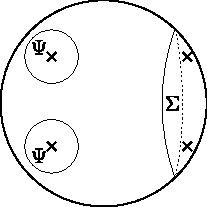
\includegraphics[width=0.3\linewidth]{V04_Psi2_Sigma.pdf}
  \caption{}
\end{figure}


A $\Sigma_n$ line of a diagram joins a $\Sigma_n$ slot of one vertex to a $\Sigma_n$ slot of another, and it carries $n$ strands, one per puncture of the slot.
Each strand is a sewing of two punctures through the inverse of the single-string pairing~\eqref{p:eq:hs1:pairing}, that is, the insertion of the level-matching bivector $b_0^- \delta_{L_0^-, 0}$ between them.
This is the sewing that produces the propagator of closed string field theory once the length of the plumbing cylinder is integrated with the insertion $b_0^+ / L_0^+$.
Here that insertion is absent: a strand is the plumbing at zero length, $w_1 w_2 = \e^{\I \theta}$, with only the twist $\theta$ integrated by the level-matching insertion, a legitimate CFT surface of measure zero in its moduli space.
A $\Psi$ line thus differs from a strand of a $\Sigma_2$ line by the integrated length alone, with its insertion $b_0^+ / L_0^+$, and not by the presence of an antighost, the level-matching insertion being common to both.
  This description holds for the pairing, and the line carries in addition the inverse $\sprod{2}{2}^{-1}$, which we discuss below.
A $\Sigma_2$ line is therefore not two strands of fixed length alone, and the surface picture of a diagram holds up to this factor.

The strands make a bookkeeping subtlety visible.
A chain of $k$ quartic vertices joined by $\Sigma_2$ lines is a tree when each line is counted as one edge, and the diagrams of \cref{p:sec:hs} are tree diagrams in this sense.
Their powers of $\gs$, their numbers of moduli and their ghost numbers are those of trees.
Resolved into punctures and strands, the same chain is the connected surface obtained by sewing $k$ spheres along $2 (k - 1)$ pairs of punctures, which has genus $k - 1$.
The two counts are reconciled by a formula that follows from the additivity of the Euler characteristic under sewing: a diagram with $L$ loops whose edges $e$ carry $k_e$ strands each has resolved genus
\begin{equation}
  \label{p:eq:ws:genus}
  g_{\mathrm{res}}
    = L + \sum_e (k_e - 1),
\end{equation}
so that a $\Sigma_2$ line raises the resolved genus by one and the loop number by zero.
No coupling and no modulus is attached to that genus, because the lengths of the necks that produce it are never integrated.
We can compare with a matrix model.
  There the double lines of a diagram fix the genus of its fat graph, and the expansion in $1 / N$ is an expansion in that genus.
  Here the strands also fix a genus, but no parameter counts it, and the physical expansion parameter $\gs$ organizes the diagrams by their loop number $L$, not by $g_{\mathrm{res}}$.

This suggests the structure of a colored operad, with one color per number of strands.
The objects are the spaces $\Hn{k}$ with their pairings $\pair[k]{\cdot}{\cdot}$.
The form $\sprod{2}{2}$ is a unary operation on the color $2$, and the cubic coupling $\vertex{4}(\Sigma_2, \Psi^2)$ is a corolla with one leg of color $2$ and two of color $1$.
Composition is the contraction of a $\Sigma_k$ line, an edge of color $k$, with the inverse of the $k$-string pairing.
The map that resolves a $\Sigma_2$ line into two ordinary strands is a linear map $\Hn{2} \hookrightarrow \Hs \otimes \Hs$ but not a map of operads, which is where the discrepancy in~\eqref{p:eq:ws:genus} comes from.
On the moduli-space side, the uncolored operad is the one of Kimura, Stasheff and Voronov on the decorated moduli spaces in which the vertex regions live~\cite{Kimura:1995:OperadStructuresModuli}.
We leave to future work the question whether the regions marked as above, together with a rule for the $\Sigma$ lines, form a colored operad of moduli spaces.
The obstacle is the line itself: its composition is not given by any kernel of the class defined below, and the one surface representation known, the Neumann series, carries algebraic factors.



The second block holds the paper's subsections on the inverse of the quartic form and on the counting of moduli.
It states three results:
\begin{itemize}
  \item there is no local worldsheet kernel for $\sprod{2}{2}^{-1}$, an exclusion within connected surfaces of bounded type carrying standard sewing ghost insertions (any genus, any number of vertices and frozen nodes, smoothed handles, continuous moduli with their $b$-ghost measure), modulo the standard input that these are the only insertions at a degenerating node: \status{Proven}\record{022-rs5-no-local-kernel-theorem (R28)};
  \item the Neumann series is a representation of $\sprod{2}{2}^{-1}$ as a convergent sum over chains of frozen-neck surfaces, under the hypothesis that the spectral radius of the iterated operator is smaller than one for the level-diagonal split, away from the zeros of the truncated determinant (\cref{ch:hypotheses}): \status{Conditional(PH21) -- Proven}\record{020-riemann-m2-geometric (R27)};
  \item the virtual dimensions of the calculus with negative moduli, for every number of punctures on the sphere, and their closure at every order: \status{Proven}\record{036-covering-m06-composite (R59)}.
\end{itemize}
The finite-model demonstration that the Neumann series can converge or diverge, while the algebraic inverse telescopes in both cases, is written out in \cref{sec:ws1:neumann}.

\subsubsection{The inverse of the quartic form}
\label{p:sec:ws:inverse}


The propagator of the auxiliary field is the inverse of a vertex, and we now ask what it means in the worldsheet description.
The propagator of the string field in Siegel gauge contains the operator $1 / L_0^+$wich can be written as a Laplace transform:
\begin{equation}
  \label{p:eq:ws:propagator-psi}
  \frac{1}{L_0^+}
    = \int_0^\infty \dd s \; \e^{- s L_0^+},
\end{equation}
This representation gives the worldsheet computation.
The operator $\e^{- s L_0^+}$ is a cylinder of length $s$, the integral over $s$ is the integral over the length of the plumbing cylinder, and $b_0^+$ is the antighost insertion that goes with that modulus.
The spectrum of $L_0^+$ is not positive, because of the tachyon, so that the RHS~\eqref{p:eq:ws:propagator-psi} does not converge, strictly speaking.
However, the LHS is perfectly well-defined and can be used as a \emph{definition} of the RHS whenever the latter is not~\cite{Sen:2015:OffshellAmplitudesSuperstring,deLacroix:2017:ClosedSuperstringField,Erbin:2021:StringFieldTheory}.

In the same spirit we write
\begin{equation}
  \label{p:eq:ws:propagator-sigma}
  \sprod{2}{2}^{-1}
    = \int_0^\infty \dd t \; \e^{- t \sprod{2}{2}},
\end{equation}
on the quotient where $\sprod{2}{2}$ is invertible, the left-hand side being the object the cubic action defines.
Making sense of the exponent needs one choice: a real positive inner product on the truncated $2$-string space, which identifies the two ghost-number sectors that the quartic form connects.
The representation~\eqref{p:eq:ws:propagator-sigma} needs in addition a sign condition on the spectrum of the quartic form in that inner product, a condition the quartic form need not satisfy.
The alternative representation $\int_0^\infty \dd t \, A \, \e^{- t A^2}$, with $A$ the real symmetric matrix of the quartic form in an orthonormal basis of that inner product, needs no such condition.
The inner product enters the integrand but not the result.
We keep the representation~\eqref{p:eq:ws:propagator-sigma} for the comparison with~\eqref{p:eq:ws:propagator-psi}, since its exponent is the quartic form itself.
  The conclusion of the next paragraph holds for the alternative as well, whose integrand expands in chains of an odd number of vertices and not term by term in the propagator.

The representation differs from~\eqref{p:eq:ws:propagator-psi} by its exponent.
In~\eqref{p:eq:ws:propagator-sigma} the exponent is the quartic form itself: there is no $L_0^+$, no $b_0^+$, and the parameter $t$ is not the length of anything.
Expanded in powers of $t$, the integrand $\e^{- t \sprod{2}{2}}$ at fixed $t$ is a sum over chains of quartic vertices joined through the inner product chosen above, which identifies the two ghost-number sectors, with the weight $(- t)^k / k!$ for the chain of $k$ vertices.
In surfaces these are chains of four-punctured spheres sewn along necks of fixed length.
The parameter $t$ is a spectral variable conjugate to the vertex, and the integral over $t$ does not commute with the expansion: each term $\int_0^\infty t^k \, \dd t$ diverges.
The representation~\eqref{p:eq:ws:propagator-sigma} therefore does not provide a term-by-term expansion of the propagator in surfaces, in contrast with~\eqref{p:eq:ws:propagator-psi}, whose integral over $s$ is part of the integral over the moduli of the sewn surface.

A representation that does expand in surfaces is the Neumann series.
Split the quartic form into its level-diagonal part and the rest,
\begin{equation}
  \label{p:eq:ws:neumann}
  \sprod{2}{2}
    = D - R,
  \qquad
  \sprod{2}{2}^{-1}
    = \sum_{k \ge 0} (D^{-1} R)^k \, D^{-1},
\end{equation}
with $D$ invertible on the quotient.
The series converges when the spectral radius of $D^{-1} R$ is below one, which we assume (and motivate below).
The term of order $k$ is a chain of $k$ insertions of $R$, the level-off-diagonal part of the quartic vertex, threaded on $k + 1$ level-diagonal $\Sigma_2$ lines $D^{-1}$.
In surfaces it is a chain of $k$ four-punctured spheres sewn pairwise along two necks of fixed length, each $\Sigma_2$ line, internal or external, carrying one algebraic factor $D^{-1}$ on its level, which acts on its pair of necks, and each sphere carrying the projection that removes the level-diagonal part of its vertex.
Where the series converges, this gives $\sprod{2}{2}^{-1}$ in terms of Riemann surfaces, up to the algebraic factors $D^{-1}$, which are not surfaces.
It is a sum over a discrete family of chains of surfaces with necks of fixed length, one algebraic factor per $\Sigma_2$ line and per vertex, rather than an integral over a continuous family.
The split~\eqref{p:eq:ws:neumann} is a choice, like a subtraction scheme, but the sum does not depend on it when it converges.
For example, for the quartic $\mathrm{SL}(2, \C)$ vertex~\cite{Erbin:2023:SL2CQuarticVertex,Erbin:2026:SL2CVerticesClosed}, on the block of pairs of zero-momentum tachyons and ghost dilatons, the spectral radius of $D^{-1} R$ is below one at the two values of the stub parameter $\beta$ checked, so the series converges there.
The matrix is not diagonally dominant on this block: the radius is below one because the products of off-diagonal entries partly cancel.
At other momenta and on the other blocks the convergence is open.
The series in $\gs$ of \cref{p:sec:hs:quintic}, which dresses $\sprod{2}{2}^{-1}$ with quintic vertices, is a Neumann series of the same kind, and its terms are chains of the same kind with quintic vertices on the line.

We can ask whether the propagator can instead be a worldsheet kernel of the usual kind, as $b_0^+ / L_0^+$ is.
By a kernel of the usual kind we mean an integral, over a finite-dimensional parameter space with a signed measure, of ghost-dressed correlators on connected surfaces with four external punctures, two in and two out.
The surfaces may have any genus and any number of nodes, the topology staying bounded over the parameter space.
They carry one antighost insertion per integrated modulus and, at each node, the standard sewing insertion: $b_0^- \delta_{L_0^-, 0}$ for a node of fixed length and $b_0^+ b_0^- / L_0^+ \, \delta_{L_0^-, 0}$ for a node whose length is integrated.
The class contains every finite connected chain of spheres sewn along necks, with the moduli of the spheres integrated or not.
The double tube, two independent plumbing cylinders, is disconnected and lies outside it.
No kernel of this class equals $\sprod{2}{2}^{-1}$, by ghost-number counting.
The inverse lowers the ghost number by two, as $\sprod{2}{2}$ raises it by two, while every correlator of the class raises it by at least two:
\begin{equation}
  \label{p:eq:ws:ghost-obstruction}
  \Ngh\big( \sprod{2}{2}^{-1} \big)
    = - 2,
  \qquad
  \Ngh\big( \text{kernel} \big)
    = 2 + \nu_f + m
    \ge 2,
\end{equation}
where $\nu_f$ is the number of nodes of fixed length and $m$ the number of unintegrated real moduli.
The second count rests on the standard factorization of CFT correlators at a node, which fixes the insertion there to the ones listed.
This is the one input of the argument, and we take it from~\cite[ch.~9]{Polchinski:2005:StringTheoryVolume} without rederiving it.
Within the class so defined the exclusion is a proof by counting, and it says nothing outside it: the insertions that could lower the ghost number, antighosts attached to no modulus, are those the class leaves out, and they are the subject of the second option below.

Outside the class lie, among others, three options.
The first is the Neumann series~\eqref{p:eq:ws:neumann}, an infinite sum with one algebraic factor per $\Sigma_2$ line and per vertex.
The second is a dressing of the surfaces by such insertions, tuned to the actual quartic vertex.
  A dressing built uniformly from the vertex data, the same construction for every vertex, is excluded by its degree: under a rescaling $\vertex{4} \to t \, \vertex{4}$ of the vertex it is homogeneous of non-negative degree in $t$, while $\sprod{2}{2}^{-1}$ has degree $- 1$.
  A dressing at the actual vertex data is not excluded by this argument.
The third is a change of the kinetic term of the auxiliary field, which is what the construction of~\cite{Erbin:2024:OpenStringStub} does for the stub of an open string field theory.
This changes the identity to be satisfied rather than the kernel.
The reading of a $\Sigma_2$ line as a surface in the previous paragraphs holds up to this one factor, which is algebraic.

\subsubsection{Counting moduli}
\label{p:sec:ws:moduli}

If a $\Sigma_2$ line carries no modulus, a diagram with such lines has fewer moduli than the vertices it is made of.
The count nevertheless matches, at every order, the dimension of the moduli space that the diagram would have to cover.
We assign to every vertex the real dimension of its region, $\hat d(\vertex{n}) = \dim_\R \mathcal V_{0,n} = 2 n - 6$, the dimension of the moduli space of the $n$-punctured sphere, extended to $n \le 2$ by the same formula.

Kinetic operators count as the vertices they are, $\hat d(Q_B) = \hat d(\vertex{2}) = - 2$ and $\hat d(\sprod{2}{2}) = \hat d(\vertex{4}) = + 2$, and the count is additive under gluing.
The dimension assigned to an inverse is then minus that of what it inverts.
For the string field this gives $\hat d(Q_B^{-1}) = + 2$, the two real moduli of the plumbing cylinder: its length, integrated with $b_0^+ / L_0^+$, and its twist, integrated by the level-matching insertion $b_0^- \delta_{L_0^-, 0}$ of the pairing.

A handle of the resolved surface~\eqref{p:eq:ws:genus} counts $- 6$, the shift of the ghost-number anomaly: $\hat d$ is the number of antighost insertions minus the number of ghost insertions minus six per resolved handle, and on a connected tree the number of integrated real moduli.
For the auxiliary field it gives
\begin{equation}
  \label{p:eq:ws:negative-moduli}
  \hat d\big( \sprod{2}{2}^{-1} \big)
    = - 2,
\end{equation}
two moduli removed rather than added.
This is the dimension-counting form of the ghost-number mismatch~\eqref{p:eq:ws:ghost-obstruction}, the two gradings agreeing on $\sprod{2}{2}$ and its inverse, and it is the sense in which a $\Sigma_2$ line carries negative moduli.
With it the count closes at every order:
\begin{equation}
  \label{p:eq:ws:closure}
  \begin{aligned}
    \hat d\big( \vertex{4} \, \sprod{2}{2}^{-1} \, \vertex{4} \big)
      &
      = 2 - 2 + 2
      = 2
      = \dim_\R \mathcal M_{0,4},
    \\
    \hat d\big( \vertex{4} \, \sprod{2}{2}^{-1} \, \vertex{5} \, \sprod{2}{2}^{-1} \, \vertex{4} \big)
      &
      = 2 - 2 + 4 - 2 + 2
      = 4
      = \dim_\R \mathcal M_{0,5},
    \\
    \hat d\big( \vertex{5} \, \sprod{2}{2}^{-1} \, \vertex{5} \big)
      &
      = 4 - 2 + 4
      = 6
      = \dim_\R \mathcal M_{0,6},
  \end{aligned}
\end{equation}
and the same closure holds for the longer chains, whose count reduces to $2 N - 6$ for $N$ external legs.
The diagrams of the cubic theory have, formally, the dimension of the moduli space with their number of external punctures, as the diagrams of closed string field theory do.
The $\Psi$-channel analogue is $\hat d(\vertex{3} \, Q_B^{-1} \, \vertex{3}) = 0 + 2 + 0 = 2$, the familiar statement that the $3$-string vertex and the propagator together have the moduli of the four-punctured sphere.
These are corollaries of the additivity of the count under gluing, and they are the same statement as the saturation of the ghost number on the sphere.

The count is necessary for a geometric reading and never sufficient, as two facts show.
The four-point chain $\vertex{4} \, \sprod{2}{2}^{-1} \, \vertex{4}$ has the dimension of $\mathcal M_{0,4}$, and it equals $\vertex{4}$ by the collapse~\eqref{p:eq:hs4:telescoping}: a chain that is a single vertex region, covering only $\mathcal V_{0,4}$.
The dimension count is satisfied there because the line removes exactly the two moduli that the second vertex region would have added, which is how the collapse shows in the count.
Conversely, the double tube, two plumbing cylinders whose lengths and twists are integrated independently, is a bona fide family of surfaces with the same count $\hat d = - 2$, and it is not the inverse.
With any signed measure over its two lengths and twists, it commutes with the two operators $L_0^\pm$ of the strands and is therefore diagonal in the $2$-string level, while $\sprod{2}{2}$ has a non-vanishing level-off-diagonal part $R$ and so has its inverse.
This excludes the double tube.
Being disconnected, it lies outside the class of~\eqref{p:eq:ws:ghost-obstruction}, whose count alone does not exclude it.

The count does not single out a surface either.
The double tube of the previous paragraph reaches $\hat d = - 2$ by the handle rule, its two cylinders sitting at resolved genus one, with no $c$-ghost insertion.
A connected surface reaches $\hat d = - 2$ only with antighost insertions attached to no modulus of its own surface, the zero modes of plumbing fixtures on its external legs, which the class of~\eqref{p:eq:ws:ghost-obstruction} does not admit.
Sewn into a diagram, they become the moduli of the two resolved handles, which is how the handle rule reaches $- 2$.
Such dressings are excluded only as uniform constructions, as said above.
A negative formal dimension is therefore not by itself an obstruction to a geometric reading, as $2$-strand families reach it through a handle.
The obstruction is the ghost-number argument~\eqref{p:eq:ws:ghost-obstruction} for connected surfaces with the standard insertions of its class, and level-diagonality for the disconnected double tube.

At six points the count is the first that is not explained by a collapse.
The composite vertex $\vertex{5 \cdot 5}$ of~\eqref{p:eq:hs5:exchange-vertex} has the dimension of $\mathcal M_{0,6}$, and it is the first chain whose line joins two interaction vertices, so that it does not collapse by the criterion of \cref{p:sec:hs:sextic:kernel}.
We call \emph{covering question} the question whether it covers a region of $\mathcal M_{0,6}$, and covers it once.
  We return to it below, after the circle picture has given the line a geometric model.
Everything in this counting is bookkeeping at a fixed level of truncation and at tree level: it gives the dimensions and says nothing about the regions themselves.



\medskip

\noindent
The next five blocks come from a note on the Riemann-surface picture of the auxiliary sector.
It derives the dictionary that the paper's worldsheet section summarizes, with the ghost-saturation diagnostic, the frozen-neck definitions, the three-grading table and the genus formula of the coloured operad.
Its results, and their status:
\begin{itemize}
  \item the two internal kernels distinguished, frozen-neck chains and their gradings, the combinatorial covering by the three exchange channels, the genus formula $g_{\rm res} = L_c + \sum_e (k_e - 1)$ of the coloured operad: \status{Proven}\record{020-riemann-m2-geometric (R27)};
  \item the identification of one contraction with the inverse single-string pairing as plumbing at frozen length, $\omega_1^{-1} = b_0^- \delta_{L_0^-, 0}$, and the factorized propagator $(b_0^+ / L_0^+) \, \omega_1^{-1}$: \status{Verified}\record{021-rs4-sewing-fixtures (R27)};
  \item the Laplace and Schwinger forms of $\sprod{2}{2}^{-1}$, under spectral conditions that are open beyond level~$0$: \status{Conditional(PH1) -- Proven} (\cref{sec:ws1:schwinger});
  \item the dictionary with the $KBc$ algebra of open string field theory is an organizing analogy, not a result, and carries no status.
\end{itemize}
The note uses an earlier notation, translated below.

\begin{quote}
  \small
  \textbf{Translation box: Riemann-surface note $\to$ paper.}
  \begin{itemize}
    \setlength{\itemsep}{0.3ex}
    \item $V_n$ $\to$ $\vertex{n}$; $V_4$ read as a bilinear form on $\Sym^2 \Hilb_0$ is the paper's $\vertex{4}(A, B) = \pair[2]{A}{\sprod{2}{2}(B)}$, and $V_4(\Sig, \Sig)$ is the kinetic term of $\Sigma_2$.
    \item $\mtwo = G_2^{-1} V_4$ $\to$ $\sprod{2}{2}$; $\mtwo^{-1}$ $\to$ $\sprod{2}{2}^{-1}$; $\Ngh(\mtwo) = + 2$ is the physical ghost number of $\sprod{2}{2}$.
    \item $\Hilb_0$ $\to$ $\Hs$ restricted to level-matched states; $\Sym^k \Hilb_0$ $\to$ $\Hn{k}$; $G_k = \omega_1^{\otimes k}$ $\to$ the multi-string pairing $\pair[k]{\cdot}{\cdot}$; $\Sig \equiv \Sigma_2$, $\Sig_k \to \Sigma_k$.
    \item The two kernels: the \enquote{worldsheet sewing kernel} $\mathsf P$ of a colour-1 line is the propagator of $\Psi$; the \enquote{colour-2 contraction} $\mathsf S = (12 / \gs^2) \, \mtwo^{-1} G_2^{-1}$ is the propagator of $\Sigma_2$ of the Feynman rules (\cref{p:sec:hs:quartic}).
    \item HS (Hubbard--Stratonovich) Feynman rules are the Feynman rules of the cubic action; $\pklg$ are the maps of the IBL structure of \cref{ch:ibl}.
    \item In the tower section, $\tilde V_{2k}(\Sig_k, \Sig_k)$ is the kinetic term of $\Sigma_k$ built from the reduced vertex, $\dvertex{2k}(\Sigma_k, \Sigma_k) = \pair[k]{\Sigma_k}{\wprod{k}{k}(\Sigma_k)}$ (\cref{ch:all-orders}); the symbols $\hat M_k$, $\hat H_k$, $L_k$ of the continued fraction are the note's own.
    \item \emph{Reality.} The note's conjugation is $\ddagger = (-1)^{\Ngh + 1} \star$ on each strand, so that its condition $\Sig_k^\ddagger = \Sig_k$ is the paper's $\Sigma_k^\star = (-1)^k \Sigma_k$: the two read the same for $\Sigma_2$, while for odd $k$ the sign is explicit, $\Sigma_3^\star = - \Sigma_3$, and $\Psi^\ddagger = \Psi$ is $\Psi^\star = - \Psi$ (\cref{ch:conventions}).
  \end{itemize}
\end{quote}

The first section of the note separates the two internal lines of a diagram, the propagator of $\Psi$ and the contraction of $\Sigma_2$, by the count of one $b$-ghost per real modulus.

\subsection{The two internal kernels}
\label{rs:sec:kernels}

The whole geometric story turns on keeping apart two objects that both look like
``an internal line'' in a Feynman graph but are worldsheet-geometrically
opposite. This section defines them and gives the sharp diagnostic --- one
$b$-ghost per real modulus --- that tells them apart.

\subparagraph{Vertices are moduli integrals; ghost saturation is the bookkeeping.}
A closed-string vertex is an integral over a vertex region of a fixed-surface
correlator with one $b$-ghost insertion per real modulus,
\begin{equation}
	V_4(A_1,\dots,A_4)
	= \int_{\mc{V}_{0,4}}\!\dd^2 m\;
	\Bra{\Sig_{0,4}(m)}\,b(v_m)\,b(\bar v_m)\,
	\ket{A_1}\otimes\cdots\otimes\ket{A_4},
	\label{rs:eq:V4integral}
\end{equation}
where $\Bra{\Sig_{0,4}(m)}$ is the four-punctured-sphere surface state at moduli
point $m$ with its chosen local coordinates, and each $b$ soaks up one real
modulus. A sphere correlator is non-zero only when the total ghost number
saturates the background charge: it needs $\Ngh=6$, and each $b$ costs one unit,
so a genus-zero $n$-point vertex on its region ($\dim_\R=2(n-3)$) is non-zero iff
\begin{equation}
	\sum_i \Ngh(A_i) \;=\; 6 + 2(n-3).
	\label{rs:eq:saturation}
\end{equation}
This is the precise sense in which \emph{one $b$-insertion per real modulus} is
the sharp diagnostic for ``is this parameter a modulus''. Every elementary vertex
of the construction saturates \eqref{rs:eq:saturation} identically, at every level
of the tower; \Cref{rs:tab:saturation} lists them. \emph{(Terminology note, sharpened
by the comparison with the closed-string sewing conventions of~\cite{Erbin:2021:StringFieldTheory}: the $b(v_m),b(\bar v_m)$ here are the Schiffer-vector
insertions soaking up a \emph{vertex-region} modulus $m$; they are distinct from
the propagator zero-modes $b_0^\pm$ of \Cref{rs:sec:frozen}. The two diagnostics
agree on the discriminant that matters: only a \emph{length}-type modulus needs a
compensating $b$; the level-matching $b_0^-\delta_{L_0^-,0}$ retained by every
frozen-neck contraction is not itself a modulus and needs no partner.)}

\begin{table}[htp]
	\centering
	\begin{tabular}{lcccc}
		\toprule
		vertex & fields ($\Ngh$ each) & $\sum\Ngh$ & $\#b = \dim_\R$ region & $\sum\Ngh-\#b$ \\
		\midrule
		$V_4(\Sig,\Sig)$ & $4,4$ & $8$ & $2$ & $6$ \\
		$V_4(\Sig,\Psi,\Psi)$ & $4,2,2$ & $8$ & $2$ & $6$ \\
		$\tilde V_{2k}(\Sig_k,\Sig_k)$ & $2k,2k$ & $4k$ & $2(2k-3)$ & $6$ \\
		$\tilde V_{2k+1}(\Sig_k,\Sig_k,\Psi)$ & $2k,2k,2$ & $4k+2$ & $2(2k-2)$ & $6$ \\
		\bottomrule
	\end{tabular}
	\caption{Ghost saturation \eqref{rs:eq:saturation} for every elementary vertex of
	the construction (the $\Ngh$ assignments are the physical ghost numbers of the products; the region
	dimensions are the standard $\dim_\R\mc{V}_{0,n}=2(n-3)$). Each row balances to
	$6$: the vertices are \emph{bona fide} moduli integrals with exactly the right
	number of $b$-insertions. This table is the diagnostic used repeatedly below:
	an internal line carries a modulus iff adding it would spoil the balance unless
	accompanied by its own $b$.}
	\label{rs:tab:saturation}
\end{table}

\subparagraph{Kernel 1: the worldsheet sewing kernel (colour-1 line).} An ordinary
closed-string internal line sews two surface states by inserting a complete set
of states weighted by the plumbing factor and integrated with the $b$-ghost
measure:
\begin{equation}
	\mathsf P
	= \int_0^\infty\!\dd s\int_0^{2\pi}\!\frac{\dd\theta}{2\pi}\;
	b_0^+\,b_0^-\;\e^{-sL_0^+ + \I\theta L_0^-}
	= \frac{b_0^+\,b_0^-}{L_0^+}\,\delta_{L_0^-,0}
	= \frac{b_0^+}{L_0^+}\,\omega_1^{-1}
	\label{rs:eq:sewing}
\end{equation}
(normalisation \textbf{verified exact} against Erbin's conventions \cite{Erbin:2021:StringFieldTheory}
including the plumbing-integral prefactor; the
factorised form separates the length-modulus factor $b_0^+/L_0^+$ from the
level-matching sewing measure $\omega_1^{-1}=b_0^-\delta_{L_0^-,0}$, identified
precisely in \Cref{rs:sec:frozen}). The point is geometric, not formal: the operator
$e^{-sL_0^+}$ \emph{is} a surface --- the CFT path integral on a flat cylinder of
length $s$ and twist $\theta$ --- and \emph{each} value of $(s,\theta)$ is a
\emph{different} surface. The double integral sweeps a two-real-parameter family
inside moduli space, and correspondingly the kernel carries exactly two
$b$-insertions, $b_0^+$ and $b_0^-$. This is how the $s$-, $t$- and $u$-channel
Feynman graphs sweep out the three propagator regions
$\mc{M}_s,\mc{M}_t,\mc{M}_u\subset\mc{M}_{0,4}$.

\subparagraph{Kernel 2: the colour-2 contraction (colour-2 edge).} Between two
$V_4(\,\cdot\,;\Psi,\Psi)$ vertices the HS Feynman rules (\cref{p:sec:hs:quartic}) insert the
\emph{state-space} kernel
\begin{equation}
	\mathsf S
	= \frac{12}{\gs^2}\,\big(V_4|_{\Sym^2}\big)^{-1}
	= \frac{12}{\gs^2}\,\mtwo^{-1}\,G_2^{-1},
	\label{rs:eq:Skernel}
\end{equation}
where $V_4|_{\Sym^2}$ is the restriction of the quartic vertex to the symmetric
square and the inverse is taken with respect to the symmetric identity. Read it
against \eqref{rs:eq:sewing}: there is \textbf{no} plumbing parameter $q$, \textbf{no}
$s$-integral, \textbf{no} \emph{length-modulus} insertion $b_0^+/L_0^+$, and
\textbf{no} $L_0^+$ (the level-matching sewing measure
$\omega_1^{-1}=b_0^-\delta_{L_0^-,0}$ \emph{per strand} is retained --- see
\Cref{rs:sec:frozen} --- it is not a length modulus). It is the inverse
of an object \eqref{rs:eq:V4integral} whose moduli have \emph{already} been
integrated. That single fact --- an inverse of an already-integrated vertex,
rather than an integral over a surface family --- is the entire geometric content
of ``$\Sig$ is auxiliary'', and everything below unpacks it.

\medskip
\noindent\emph{Physical meaning.} The distinction is not bookkeeping pedantry.
Kernel 1 is a \emph{generator} of geometry: sliding $s$ deforms the worldsheet
continuously, and the pole at $L_0^+=0$ (from $\int_0^\infty\dd s\,\e^{-sL_0^+}$)
is an on-shell propagating state. Kernel 2 is a \emph{finished, rigid} object: it
appends no length, deforms no surface, and has no $s\to\infty$ degeneration to
produce a pole. The exchanged $\Sig$ therefore never goes on-shell --- it is
auxiliary --- and the reason is the \emph{absence of a length modulus}
($b_0^+/L_0^+$) on its line, not the boundedness of one; the retained
$b_0^-\delta_{L_0^-,0}$ is the universal level-matching measure common to every
closed-string line, propagating or contact, and does not by itself signal a
modulus. \emph{(The kernel \eqref{rs:eq:Skernel} is the $\Sig$ line of the Feynman rules; the open-string stub mechanism of \cref{ch:qft-toys} belongs to a different construction and does not apply here; the length-vs-level-matching
distinction is checked against the closed-string sewing conventions of~\cite{Erbin:2021:StringFieldTheory}.)}



The second section defines frozen-neck sewing, shows that a colour-2 edge is two such contractions at once, computes the resolved genus of a chain, and shows in the three-grading table that the physical gradings follow the coloured graph.

\subsection{Frozen-neck sewing and the chain surfaces}
\label{rs:sec:frozen}

We now ask what surface, if any, sits behind a single colour-2 contraction, and
what a chain of them looks like. The answer is a legitimate but measure-zero
surface, and a chain is a \emph{discrete} family, in sharp contrast to the
continuous family swept by \eqref{rs:eq:sewing}.

\subparagraph{A single bare contraction is frozen-neck sewing.} Before inverting
anything, consider the bare pairing $G_2^{-1}=\omega_1^{-1}\otimes\omega_1^{-1}$
inserted between two surface states. The sewing theorem says that inserting a
complete set $\sum_a\ket{\phi_a}\bra{\phi^a}$ at a pair of punctures, dressed with
the plumbing weight $q^{L_0}\bar q^{\bar L_0}$ and integrated with the $b$-ghost
measure, glues the two surfaces into one with neck modulus $q$ and reproduces the
family \eqref{rs:eq:sewing}. Dropping the \emph{length}-modulus weight --- fixing
$s=0$ (equivalently $|q|=1$), with no $s$-integration and no $b_0^+$ --- still
glues the surfaces, but into a \emph{single point} of the larger moduli space
rather than a family. In words: \emph{ordinary} plumbing sews two punctures and
then \emph{lets the neck stretch}, sweeping out a whole family of surfaces as $s$
varies; a \emph{frozen-neck} contraction sews the same two punctures but the neck
never stretches --- $s$ is pinned at $0$, so exactly one surface comes out, not a
family. \textbf{Checked against the closed-string sewing conventions of~\cite{Erbin:2021:StringFieldTheory}}:
the sum $\sum_a\ket{\phi_a}\bra{\phi^a}$, with the $\omega_1$-dual $\bra{\phi^a}$,
is \emph{exactly} the bivector $\omega_1^{-1}=b_0^-\delta_{L_0^-,0}$ --- since
$\omega_1(A,B)=\Mean{A|c_0^-|B}$ and $\{c_0^-,b_0^-\}=1$ on $\ker b_0^-$, so
$b_0^-c_0^-=\id$ there. This retains \emph{one} $b$-ghost ($b_0^-$) plus the
level-matching projector; what is genuinely dropped relative to the full
propagator \eqref{rs:eq:sewing} is only the length-modulus factor $b_0^+/L_0^+$.
Hence:
\begin{definition}[Frozen-neck contraction]
	\label{rs:def:frozenneck}
	A \emph{frozen-neck contraction} between two punctures is the gluing obtained
	from the ordinary plumbing construction \eqref{rs:eq:sewing} by fixing the length
	modulus at $s=0$ (equivalently $|q|=1$) instead of integrating over it, and
	omitting the length-modulus factor $b_0^+/L_0^+$ (the $b_0^+$ ghost and the
	Schwinger integral $\int\dd s\,\e^{-sL_0^+}$), while retaining the
	level-matching sewing measure $b_0^-\delta_{L_0^-,0}$. Concretely, it is
	insertion of the bivector
	$\omega_1^{-1}=\sum_a\ket{\phi_a}\bra{\phi^a}=b_0^-\delta_{L_0^-,0}$ at the two
	punctures, with \emph{no} $q^{L_0}\bar q^{\bar L_0}$ length weight and
	\emph{no} $\int\dd s$.
\end{definition}
\begin{quote}
	\textbf{Frozen-neck identification.} \emph{One $\omega_1^{-1}=b_0^-\delta_{L_0^-,0}$ contraction
	between two punctures is plumbing with the \textbf{length} modulus frozen
	(\Cref{rs:def:frozenneck}, no $b_0^+/L_0^+$), retaining the level-matching
	sewing measure: a legitimate CFT surface, of measure zero in its moduli
	space.} \emph{(Checked against the sewing conventions of~\cite{Erbin:2021:StringFieldTheory}
	--- cross-checked two independent ways [operator factorisation
	of Erbin's $K\Delta=1$, and explicit ghost zero-mode matrices] plus a
	finite-dimensional check. The discriminant between a colour-1
	(propagating) and colour-2 (contact) line is the \emph{length}-modulus
	$b_0^+/L_0^+$, not the presence of any $b$-ghost whatsoever --- the retained
	$b_0^-\delta_{L_0^-,0}$ is common to both. Remaining open item: $|q|=1$
	sewing for the \emph{stubbed} vertex local coordinates converges via the
	stub's $\e^{-\frac{s_0}2 L_0^+}$ suppression at an effective neck $s_0>0$,
	consistent-with the book's plumbing range, not independently re-derived from
	scratch here.)}
\end{quote}
A colour-2 edge (\Cref{rs:def:colour2edge} below) is built from \emph{two} such
contractions at once, one per puncture of the pair; a chain (\Cref{rs:def:chain}
below) is built by iterating them along a sequence of vertex regions. Both
inherit the frozen-neck identification above: they are honest, CFT-verified surfaces at
the level of the sewing formalism, with the length-frozen,
level-matching-retained fixture just established.

\subparagraph{A colour-2 edge is two contractions at once; it fixes the genus.}
\begin{definition}[Colour-2 edge]
	\label{rs:def:colour2edge}
	A \emph{colour-2 edge} between two $V_4(\Sig,\Psi,\Psi)$ vertex regions is a
	pair of simultaneous frozen-neck contractions (\Cref{rs:def:frozenneck}), one at
	each of the two punctures carrying the $\Sig\in\Sym^2\Hilb_0$ leg. Equivalently,
	it is insertion of the bivector
	$G_2^{-1}=\omega_1^{-1}\otimes\omega_1^{-1}
	=(b_0^-\delta_{L_0^-,0})^{\otimes2}$ between the two vertices'
	$\Sig$-punctures: two $b_0^-$'s (one per strand), no $b_0^+/L_0^+$.
\end{definition}
The Euler characteristic is additive under sewing.
Gluing two four-punctured spheres ($\chi=-2$ each, total $\chi=-4$) over two
puncture pairs leaves $n_{\rm ext}=4$ external punctures, so from
$\chi=2-2g-n_{\rm ext}$,
\begin{equation}
	-4 = 2-2g-4 \quad\Longrightarrow\quad g=1.
	\label{rs:eq:g1}
\end{equation}
The resolved surface behind one colour-2 edge is therefore a \emph{genus-one}
surface, frozen at a point of its neck moduli.

\begin{definition}[Length-$k$ chain]
	\label{rs:def:chain}
	A \emph{length-$k$ chain} is the surface obtained by joining $k$ copies of the
	four-punctured-sphere vertex region $\mc{V}_{0,4}$ in series with $k-1$
	colour-2 edges (\Cref{rs:def:colour2edge}): vertex $1$'s $\Sig$-pair is
	frozen-neck-contracted to vertex $2$'s, vertex $2$'s remaining $\Sig$-pair to
	vertex $3$'s, and so on, leaving the $4$ punctures at the two ends of the chain
	(one $\Sig$-pair from vertex $1$, one from vertex $k$) uncontracted as the
	external legs. Equivalently, a length-$k$ chain is the surface underlying one
	term of the operator $\mtwo^{k-1}$ (\Cref{rs:eq:m2squared} below spells out
	$k=2$).
\end{definition}
\emph{Worked example.} A length-$2$ chain is a single colour-2 edge joining two
$\mc{V}_{0,4}$'s: by \eqref{rs:eq:g1}, $g=1$, a once-punctured-torus-like handle
frozen at one point of its neck modulus, with $4$ external legs ($2$ from each
vertex) and $1$ unfrozen modulus \emph{per vertex} ($2$ complex moduli total,
i.e.\ $m$ and $m'$ each ranging over $\mc{V}_{0,4}$). A length-$3$ chain adds one
more vertex and one more colour-2 edge: $\chi=-2-2-2=-6$, $n_{\rm ext}=4$, so
$2-2g-4=-6\Rightarrow g=2$; three unfrozen vertex moduli, two frozen necks. In
general, for a chain of $k$ vertices joined by $k-1$ colour-2 edges the same
count gives $\chi=-2k$, $n_{\rm ext}=4$, hence
\begin{equation}
	g=k-1,
	\label{rs:eq:chaingenus}
\end{equation}
this is the two-gradings statement of \cref{sec:ws1:grading}, now with its surface identified. The
chain is a family of genus-$(k-1)$ surfaces whose only unfrozen moduli are the
$k$ vertex-region moduli (a measure-zero slice of $\mc{M}_{k-1,4}$, whose complex
dimension is $3k-2$, for $k\ge2$: at $k=2$ that slice is $2$ real dimensions out
of $3\cdot2-2=4$ complex $=8$ real). See \Cref{rs:fig:chain}.

\subparagraph{Why the genus is formal: the three-grading table.} The physical
gradings all follow the \emph{coloured} graph (edge = one edge), not the resolved
surface. \Cref{rs:tab:grading} tabulates the mismatch for a chain of $k$ vertices. In
every row the resolved-surface prediction would attach a cost --- a $\gs$-power, a
$b$-insertion, a modulus --- to a handle that the amplitude never pays for,
because the neck is frozen and never integrated. This is the 't~Hooft double-line
situation \cite{tHooft1974} run in reverse: the ribbon (resolved) genus exists as
Euler-characteristic bookkeeping, but no coupling is attached to it. In the
physical (coloured) grading the chain is a \emph{tree}, $L_c=E-V+1=0$.

\begin{table}[htp]
	\centering
	\begin{tabular}{p{0.16\linewidth}p{0.37\linewidth}p{0.37\linewidth}}
		\toprule
		grading & resolved-surface prediction (chain of $k$) & actual (HS Feynman rules) \\
		\midrule
		coupling
		& $\gs^{2g}=\gs^{2(k-1)}$ relative suppression at genus $g=k-1$
		& uniform $\gs^{2}$: $k$ vertices ($\gs^2$ each) $\times$ $(k{-}1)$ propagators ($\gs^{-2}$ each) \\
		moduli / $b$-count
		& $2(3k-2)$ real moduli, $2(3k-2)$ $b$'s
		& $2k$ real moduli ($k$ vertex regions), $2k$ $b$'s; the $2(2k-2)$ neck moduli and their $b$'s are absent \\
		ghost number
		& ---
		& $\Ngh(\pklg)=3\ell-2k+g$ on the coloured tree \\
		\bottomrule
	\end{tabular}
	\caption{The three physical gradings of a length-$k$ chain follow the coloured
	graph, not the resolved genus-$(k-1)$ surface. The
	discrepancy is the double-line phenomenon \cite{tHooft1974}: the resolved
	handle exists as $\chi$-bookkeeping but carries no coupling because its neck
	moduli are never integrated.}
	\label{rs:tab:grading}
\end{table}

\subparagraph{$\mtwo$ as an integral operator; $\mtwo^n$ as a discrete family.}
Raising the indices of \eqref{rs:eq:V4integral} with the frozen-neck bivectors,
$\mtwo=G_2^{-1}V_4$ is the integral operator
\begin{equation}
	\mtwo = \int_{\mc{V}_{0,4}}\!\dd^2 m\; K(m),
	\qquad
	K(m) = \big(\omega_1^{-1}\otimes\omega_1^{-1}\big)\,
	\Bra{\Sig_{0,4}(m)}\,b\,\bar b,
	\label{rs:eq:m2integral}
\end{equation}
one fixed surface per moduli point. Composition uses the frozen-neck identification: the product of two
such operators is the frozen-neck gluing of their surfaces,
\begin{equation}
	\mtwo^2
	= \int_{\mc{V}_{0,4}}\!\!\int_{\mc{V}_{0,4}}\!\dd^2 m\,\dd^2 m'\;
	K(m)\,K(m'),
	\qquad
	K(m)\,K(m') = \big[\,\Sig(m)\,\#_{q=1}\,\Sig(m')\,\big]^{\sharp},
	\label{rs:eq:m2squared}
\end{equation}
a genus-one frozen-neck surface, and generally $\mtwo^n$ is the integral over the
$n$ vertex moduli of the genus-$(n-1)$ frozen-neck chain. The key structural fact:
\begin{quote}
	\textbf{Discrete chains.} \emph{$\{\mtwo^n\}_{n\ge0}$ is a \textbf{discrete} semigroup of
	(families of) surfaces, graded by chain length $n$, with
	$\mtwo^n\,\mtwo^{n'}=\mtwo^{n+n'}$ realised by frozen-neck concatenation.
	Contrast $\{e^{-sL_0^+}\}_{s\ge0}$: a \textbf{continuous} semigroup, graded by
	cylinder length, with $s+s'$ realised by cylinder concatenation.}
\end{quote}
This is the precise content of the word ``contact''. The operator $L_0^+$ is the
\emph{generator} of a geometric flow --- each instant of Schwinger time $s$
deforms the surface --- whereas $\mtwo$ is a \emph{finished surface}: each
application appends one complete, already-integrated vertex region through a rigid
neck. There is no operator whose exponential flow grows $\mc{V}_{0,4}$ out of a
point; the vertex region is an input of the construction, not an orbit.

\medskip
\noindent\emph{Physical meaning and a $b$-ghost check.} In
$e^{-t\mtwo}=\sum_n\frac{(-t)^n}{n!}\mtwo^n$ the parameter $t$ multiplies
\emph{fixed} chains by scalar weights: varying $t$ re-weights the discrete family
and deforms no geometry. Thus $t$ is Laplace-dual to the interaction data
$\spec(\mtwo)$, exactly as $s$ is Laplace-dual to the worldsheet energies
$\spec(L_0^+)$. The diagnostic of \Cref{rs:tab:saturation} confirms the reading: the
$s$-integral of \eqref{rs:eq:sewing} carries $b_0^+$, whereas a $t$-integral carries
no $b$; were $t$ a modulus, the saturation \eqref{rs:eq:saturation} would fail by one
unit on every $\Sig$-exchange. \emph{(See \cref{sec:ws1:schwinger}; the reading is structural,
resting on the frozen-neck identification.)}



The third section makes the colour-2 edge exact as a composition in a coloured operad and proves the genus formula.

\subsection{A coloured operad: two punctures glued without raising the genus}
\label{rs:sec:operad}

The cleanest way to make ``a colour-2 edge glues two pairs of punctures without
raising the genus'' precise, rather than paradoxical, is to choose objects for
which it is true by construction. The device is a multi-sorted (coloured) operad,
in which the symmetric square is a \emph{single} colour rather than a pair of
ordinary punctures.

\subparagraph{Objects, operations, and the resolution functor.} Take colours
\begin{equation}
	C_1=\Hilb_0,\quad C_2=\Sym^2\Hilb_0,\quad\dots,\quad C_k=\Sym^k\Hilb_0,
	\qquad \Ngh(C_k)=2k,
	\label{rs:eq:colours}
\end{equation}
each with its own pairing ($\omega_1$ on $C_1$; $G_k=\omega_1^{\otimes k}$ on
$C_k$). Then $\mtwo$ is a \emph{unary} operation $C_2\to C_2$; the HS vertex
$V_4(\Sig,\Psi,\Psi)$ is a $(C_2;C_1,C_1)$-corolla; the cobracket $p_{1,2,0}$ is a
colour-changing unary $C_1\to C_2$; and composition is contraction of one
$C_k$-edge with $G_k^{-1}$. In this category a colour-2 edge is \emph{one} edge, a
tree is a tree, and the genus is the coloured loop number $L_c=E-V+1$. The ``two
punctures at once'' of the strand picture is the \emph{resolution functor}
$\rho:C_2\hookrightarrow C_1\otimes C_1$, a morphism of vector spaces that is
\textbf{not} a morphism of the graded operadic structures: it fails to preserve
exactly the three gradings of \Cref{rs:tab:grading}.

\subparagraph{The genus formula.} Let $E_s=\sum_e k_e$ be the total number of
elementary strand-sewings across the coloured edges $e$ (a colour-$k$ edge is a
$k$-strand cable, contributing $k$ sewings), $V$ the number of vertices, and
$L_c=E-V+1$ the coloured loop number ($E$ = number of coloured edges), for a
\emph{connected} coloured graph all of whose vertices are genus-zero. Then
\begin{empheq}[box=\fbox]{equation}
	g_{\rm res} = E_s - V + 1 = L_c + \sum_e (k_e-1).
	\label{rs:eq:genus}
\end{empheq}
\emph{Derivation (three lines, proven here).} (1) The Euler characteristic is
additive under sewing and each strand-sewing preserves the total
$\chi=\sum_v(2-n_v)$, where $n_v$ is the valence of vertex $v$. (2) With
$n_{\rm ext}=\sum_v n_v-2E_s$ external legs and $\chi_{\rm res}=2-2g_{\rm res}-n_{\rm ext}$,
equate: $2-2g_{\rm res}-\big(\sum_v n_v-2E_s\big)=\sum_v(2-n_v)=2V-\sum_v n_v$. (3)
The $\sum_v n_v$ cancels, leaving $2-2g_{\rm res}+2E_s=2V$, i.e.
$g_{\rm res}=E_s-V+1$; substituting $E_s=E+\sum_e(k_e-1)$ and $L_c=E-V+1$ gives the
second equality. \qed

\medskip
\noindent The physical (coloured) grading uses $L_c$; the resolved (formal) genus
exceeds it by $k_e-1$ per colour-$k$ edge. \textbf{A colour-2 edge raises the
resolved genus by one and the physical genus by zero} --- this is
\eqref{rs:eq:g1} for a single edge and $g=k-1$ for a chain (\Cref{rs:tab:grading}). The
discrepancy is not a paradox: it is precisely the statement that $\rho$ is not a
map of operads.

\subparagraph{The CFT-data formula for the composition.} Contracting a $C_2$-edge
inserts, at two punctures of one vertex region and two of another, the fixed
(moduli-independent) two-string state sandwich
\begin{equation}
	\sum_{a,b,c,d}\big(V_4^{-1}\big)^{(ab),(cd)}\;
	\ket{\phi_a}\ket{\phi_b}\otimes\ket{\phi_c}\ket{\phi_d}.
	\label{rs:eq:c2insert}
\end{equation}
Compare the colour-1 insertion \eqref{rs:eq:sewing}, which is
$\sum_a\int\dd s\,\dd\theta\;e^{-sh_a+\I\theta\bar h_a}\,(b\text{-dressed})\,
\ket{\phi_a}\bra{\phi^a}$. The difference between the two kernels --- the presence
versus absence of the $(s,\theta)$ family and its $b$'s --- \emph{is} the entire
geometric distinction between propagating and auxiliary, and it sits in the edge
kernel, not in the vertices. See \Cref{rs:fig:kernels}.

\subparagraph{Where this sits in the operad literature.} Multi-edge gluings between
two vertices are exactly what \emph{properads} grade by graph genus
\cite{Vallette2007}; treating $\Sym^2\Hilb_0$ as a single colour converts the
double-edge gluing into a \emph{dioperadic} (single-edge, tree-level) composition
\cite{Gan2003}. The ambient framework for surfaces with in- and out-punctures at
all genera is the modular operad of Getzler--Kapranov \cite{GetzlerKapranov1998}.
The HS construction chooses the dioperadic description, and the amplitudes agree
with that choice (\Cref{rs:tab:grading}). \emph{(Interpretive: the operad statements
are an organising language for the gradings established above, not an independent
theorem.)}



The fourth section compares the auxiliary sector with the analytic-solution technology of open string field theory, entry by entry.

\subsection{The open-string \texorpdfstring{$KBc$}{KBc} dictionary}
\label{rs:sec:osft}

We now compare with Witten's open-string product and with the analytic
($KBc$) solution technology. The analogy is tight and entry-by-entry, and it does
useful work: it shows that manipulating a non-geometric object like $\mtwo^{-1}$
is exactly the closed-string counterpart of the wedge-algebra bookkeeping that
makes analytic solutions well-defined, and it locates the one genuinely open
question on the closed side.

\subparagraph{The $KBc$ algebra in one paragraph.} The analytic-solution technology
of open SFT \cite{Schnabl2005,ErlerSchnabl2009,Erler2019} is built on the algebra
$K,B,c$: $K$ \emph{generates} worldsheet strips, so $e^{-tK}$ is a wedge of width
$t$ (one surface per $t$, a continuous semigroup); $B$ is its $b$-ghost partner;
$c$ a boundary insertion. \Cref{rs:tab:osft} gives the entry-by-entry
correspondence.

\begin{table}[htp]
	\centering
	\renewcommand{\arraystretch}{1.3}
	\begin{tabular}{p{0.42\linewidth}p{0.42\linewidth}}
		\toprule
		open string ($KBc$) & closed HS \\
		\midrule
		$K$: strip \emph{generator}; $e^{-tK}$ = one surface per $t$ (continuous semigroup)
		& $L_0^+$: cylinder generator; $e^{-sL_0^+}$ = one surface per $s$ (both geometric) \\
		Witten $*$: half-string overlap, moduli-free vertex; covers $\mc{M}$ with $1/K$ alone \cite{GiddingsMartinecWitten1986}
		& vertex regions $\mc{V}_{0,n}$: moduli-free \emph{as vertices} (moduli pre-integrated); do \textbf{not} cover $\mc{M}$ alone (Sonoda--Zwiebach) --- hence the tower \\
		wedge algebra $e^{-t_1K}e^{-t_2K}=e^{-(t_1+t_2)K}$: width additive, continuous
		& chain monoid $\mtwo^{n}\mtwo^{n'}=\mtwo^{n+n'}$: length additive, \textbf{discrete} (\cref{rs:sec:frozen}) --- the central structural analogy \\
		$\dfrac{1}{1+K}=\int_0^\infty\!\dd t\,e^{-t}e^{-tK}$: geometric, every fibre an honest positive-width strip
		& $\mtwo^{-1}=\sum_n (D^{-1}N)^nD^{-1}$ \eqref{p:eq:ws:neumann}: ``geometric'', every term an honest frozen-neck chain \\
		inverse wedge $e^{+K}$ (``negative width''): formal, non-geometric; legal only with net positive width, $e^{K}e^{-2K}=e^{-K}$
		& $\mtwo^{-1}$ bare: formal, non-surface (\cref{p:sec:ws:inverse}); legal sandwiched, $V_4V_4^{-1}V_4=V_4$ \eqref{p:eq:hs4:telescoping} \\
		$1/K$ dangerous: $\spec(K)$ reaches $0$ (sliver); needs the security strip / phantom terms
		& $1/\mtwo$ conditional: $\spec(\mtwo)$ bounded from $0$ (\cref{ch:momentum-space}); kernel quotiented \\
		\bottomrule
	\end{tabular}
	\caption{The open-SFT $KBc$ dictionary. Left column: literature
	\cite{Schnabl2005,ErlerSchnabl2009,Erler2019,GiddingsMartinecWitten1986}.
	Right column: results of \cref{p:sec:hs:quartic,p:sec:ws:inverse,sec:ws1:schwinger}. The correspondence itself is an
	organising analogy, not a theorem.}
	\label{rs:tab:osft}
\end{table}

\subparagraph{Two uses of the dictionary.} \emph{(a)} It says exactly what an
analytic-solution practitioner means by manipulating non-geometric elements: what
the telescoping~\eqref{p:eq:hs4:telescoping} licenses --- formal inverses are permitted whenever the full expression
telescopes to net-geometric objects, and the amplitude identity \eqref{eq:ch2:amp:sum}
is the closed-string counterpart of the wedge-width bookkeeping that makes
solutions of the type $\psi=\frac{1}{1+K}c(1+K)Bc\frac{1}{1+K}$ well-defined.
\emph{(b)} It locates the genuinely open question: Erler-style control of
$1/(1+K)$ rests on $\spec(K)\ge0$; the closed analogue --- positivity or a gap of
$\mtwo$ on $\Sym^2\Hilb_0$ --- is the question of \cref{ch:momentum-space}, and the dictionary suggests
importing the OSFT toolkit (resolvent estimates, level-truncated spectral density)
rather than seeking a worldsheet representation of $\mtwo^{-1}$ that, by
\cref{p:sec:ws:inverse}, does not exist in the class of local kernels defined there. \emph{(Interpretive: the OSFT-side facts are
literature, the closed-side facts are the results cited in the table, the correspondence is an
analogy.)}



The fifth section extends the dictionary to the tower of fields $\Sigma_k$ of the all-orders construction.

\subsection{The \texorpdfstring{$\Sig_k$}{Sigma_k} tower}
\label{rs:sec:tower}

The all-orders construction (\cref{ch:all-orders}) adds, per level $k$: a kinetic
vertex $\tilde V_{2k}(\Sig_k,\Sig_k)$, an odd coupling
$\tilde V_{2k+1}(\Sig_k,\Sig_k,\Psi)$, and a source $L_k$ coupling $\Sig_{k-1}$ to
$\Sig_k$. Everything in \cref{rs:sec:kernels,rs:sec:frozen,p:sec:ws:inverse,rs:sec:operad,rs:sec:osft}, and in the three-channel collapse of \cref{sec:order:amplitude},
extends verbatim with the colour set $\{C_k\}$. See \Cref{rs:fig:cable,rs:fig:tower}.

\begin{itemize}[leftmargin=*]
	\setlength{\itemsep}{1ex}

	\item \textbf{Edges are $k$-strand cables.} A colour-$k$ edge contracts
	$G_k^{-1}$, i.e. $k$ simultaneous frozen-neck sewings; by \eqref{rs:eq:genus} it
	adds $k-1$ to the resolved genus and $0$ to the physical one. A single $\Sig_3$
	edge already hides a frozen genus-$2$ surface (\Cref{rs:fig:cable}). The
	coloured-tree cubic action thus resums, at order $\gs^{2K}$, frozen
	configurations of resolved genus up to $\sum_e(k_e-1)$ --- with no $\gs$-cost,
	no neck moduli, no $b$'s: the three-grading table certifies the coloured
	reading at every $k$.

	\item \textbf{Vertex regions.} $\tilde V_{2k}$ lives on a (dressed) region
	$\mc{V}_{0,2k}$ with $\dim_\R=2(2k-3)$, and the saturation
	\eqref{rs:eq:saturation} holds identically at every $k$ (last two rows of
	\Cref{rs:tab:saturation}): the tower is ghost-consistent as a family of
	\emph{bona fide} elementary vertex regions.

	\item \textbf{Dressing = amputated colour-2 subtrees.} The dressed kernel
	$\tilde V_{2k}=V_{2k}+(\text{terms containing }V_4^{-1},\dots)$ is, in coloured-graph
	language, the bare $2k$-punctured region \emph{minus} its colour-reducible
	parts --- ``vertex $=$ amplitude minus exchanges'', now at the level of kernels
	with frozen necks, which is why no moduli bookkeeping accompanies the
	subtraction (\cref{ch:all-orders}).

	\item \textbf{The continued fraction is nested telescoping.} The recursion of the matching theorem (\cref{ch:all-orders})
	\begin{equation}
		\hat H_k
		= \hat M_k
		- \gs^2\,\frac{(2k)!}{(2k+2)!}\,L_{k+1}^\top\,\hat H_{k+1}^{-1}\,L_{k+1}
		\label{rs:eq:cfrac}
	\end{equation}
	reads geometrically as: the effective colour-2 kernel at level $k$ is the
	level-$k$ vertex region corrected by chains passing through ever-higher strand
	numbers. Every $\hat H_{k+1}^{-1}$ appears sandwiched between $L_{k+1}$'s, so
	the whole fraction telescopes to contact support --- the all-orders version of
	\eqref{eq:ch2:amp:sum}. Convergence in $\gs$ of the infinite fraction (an open
	item) is the tower analogue of the spectral condition of \Cref{rs:sec:osft}(b).
\end{itemize}

\medskip
\noindent\emph{Physical meaning.} The tower does not introduce any new
\emph{geometric} ingredient: each new level is another colour, another rigid
cable, another frozen-neck contraction. The entire content of ``a cubic action
exists at every order'' is that all the higher-genus \emph{resolved}
surfaces it silently resums are frozen and unpaid-for --- the physical expansion
stays a coloured tree. \emph{(The geometric reading is
structural, inheriting the frozen-neck identification at every $k$.)}



% ------------------------------------------------------------------
\subsection{The inverse of the quartic form: gradings, Schwinger forms, Neumann series}
\label{sec:ws1:inverse-full}

\status{mixed}\record{008-a2-v4-inverse-analysis (R15)}
The coloured grading of chains \status{Proven}; the Schwinger forms of the inverse of the Gram matrix, with the collapse in sandwiched position \status{Proven}; the level-$0$ anchor, a nonvanishing tachyon-diagonal element \status{Numerical}.

This section gives the derivations behind three statements of the paper's subsection on the inverse: that a chain of $\Sigma_2$ exchanges is graded by the coloured graph and not by the genus of its resolution, that the inverse has a Schwinger form whose parameter is not a modulus, and that the Neumann series is the one place where the four-point identity of \cref{sec:order:amplitude} can fail.
Throughout, we work at a fixed truncation level, so that $\Hn{2}$ is finite-dimensional, and we use the Feynman rules of the quartic order (\cref{p:sec:hs:quartic}): the $\Sigma_2$ propagator is $(12 / \gs^2) \, \sprod{2}{2}^{-1}$, acting on the quotient by the kernel of $\sprod{2}{2}$, and every field of this sector is Grassmann even in the physical grading.
The total symmetry of $\vertex{4}$ in its four slots is used where stated.

\subsubsection{Two gradings of a chain}
\label{sec:ws1:grading}

We describe the diagrams in two colours: colour~$1$ is a single-string leg, carrying $\Hs$, and colour~$2$ is a double-string leg, carrying $\Hn{2}$.
The ingredients of the cubic action are then coloured corollas: $\vertex{3}(\Psi^3)$ is a corolla $(1, 1, 1)$; $\vertex{4}(\Sigma_2, \Psi^2)$ is a corolla $(2, 1, 1)$, the four-punctured sphere with two of its punctures bundled into one colour-$2$ leg; the kinetic term $- \tfrac{\gs^2}{4!} \vertex{4}(\Sigma_2, \Sigma_2)$ is a corolla $(2, 2)$.
A colour-$1$ edge is ordinary plumbing with the propagator of $\Psi$.
A colour-$2$ edge is a contraction with the propagator of $\Sigma_2$, one elementary composition, which we draw as a double line.
The coloured loop number of a connected diagram counts the edges of both colours, each as one edge,
\begin{equation}
  \label{eq:ch9:coloured-loops}
  L_c
    = E - V + 1.
\end{equation}

Consider a chain of length $k$: $k$ corollas of type $(2, 1, 1)$ or $(2, 2)$ joined linearly by $k - 1$ colour-$2$ edges.
This is the power $\vertex{4}^k$ that appears in any expansion of the inverse, a Neumann or a Schwinger series.
In the coloured grading it is a tree: $E = k - 1$, $V = k$, $L_c = 0$.
Its underlying uncoloured surface is obtained by resolving each colour-$2$ edge into two simultaneous ordinary plumbings, so that $k$ four-punctured spheres are glued along $2 (k - 1)$ necks.
Gluing along circles preserves the additivity of the Euler characteristic, since $\chi(S^1) = 0$, and
\begin{equation}
  \label{eq:ch9:chain-genus}
  \chi
    = \sum_{i = 1}^k \chi(S^2 \smallsetminus 4 \text{ points})
    = - 2 k,
  \qquad
  n_{\rm ext}
    = 4 k - 4 (k - 1)
    = 4,
  \qquad
  2 - 2 g - n_{\rm ext}
    = \chi
  \;\Longrightarrow\;
  g
    = k - 1.
\end{equation}
Both computations are correct, and they grade different things.
The genus $k - 1$ is a formal Euler-characteristic bookkeeping of a resolution of the chain into surfaces with fixed, degenerate plumbing: the moduli of genus $k - 1$ with four punctures, of complex dimension $3 g - 3 + n = 3 k - 2 > 0$ for $k \ge 2$, never appear, since the chain carries no moduli integral beyond those of its vertices.
The perturbative expansion of the auxiliary theory, its power counting in $\gs$ and its split into trees and loops are governed by $L_c$.

The power counting shows why.
With $\vertex{4}$ of order $\gs^2$ and the propagator of order $\gs^{-2}$, the chain of length $k$ carries
\begin{equation}
  \label{eq:ch9:chain-coupling}
  \gs^{2 k} \cdot \gs^{- 2 (k - 1)}
    = \gs^2,
\end{equation}
the order of one $\vertex{4}$.
This is a consistency requirement rather than an independent argument, since the chains resum to $\vertex{4}$ by the telescoping in sandwiched position.
The inferential content is the contrapositive: a grading by the uncoloured genus would predict a suppression $\gs^{2 (k - 1)}$ of the chain of length $k$, which contradicts the actual uniform $\gs^2$.
The uncoloured grading is therefore inconsistent with the coupling expansion, and the coloured grading agrees with it.

\paragraph{Physical meaning.}
A $\Sigma_2$ exchange is a tree-level event however much genus its resolution carries, in the same way as a nonplanar contraction in a matrix model is still a tree diagram of the matrix field: the double line of 't~Hooft~\cite{tHooft1974} carries a ribbon genus to which no coupling is attached.
The statement does not say that the coloured composition is a geometric sewing of a new class of surfaces with coloured punctures; the coloured operad of the Riemann-surface note makes the composition exact as an operation on state spaces, not as a sewing.

\subsubsection{Schwinger forms of the inverse}
\label{sec:ws1:schwinger}

To speak of a spectrum we choose an auxiliary positive-definite inner product $G$ on $\Hn{2}$, for instance the Euclidean product of a level truncation, and write $A$ for the matrix of $\vertex{4}$ restricted to $\Hn{2}$ in an orthonormal basis of $G$.
We assume that $A$ is real symmetric, which uses the total symmetry of $\vertex{4}$, and invertible on the quotient by the kernel.
The choice of $G$ is not canonical: the BPZ pairing is not positive definite, and in infinite dimensions the self-adjointness of $A$ depends on the choice.
The question whether the vertex form is positive definite is therefore a question about the pair $(\vertex{4}, G)$, the operator tested being $G^{-1} \vertex{4}$, and not about the vertex alone.
Only the form inverse that enters the propagator is canonical, and it is recovered as $(G^{-1} \vertex{4})^{-1} G^{-1}$.
Nothing physical depends on the choice, because the collapse~\eqref{eq:ch9:sandwich} below does not involve $G$.
The statements are finite-dimensional; their extension to infinite dimensions needs $A$ self-adjoint with $0$ outside its spectrum, which we do not establish.

\paragraph{Direct form.}
The heat-kernel form holds only for a positive spectrum,
\begin{equation}
  \label{eq:ch9:schwinger-direct}
  A^{-1}
    = \int_0^\infty \dd t \, \e^{- t A}
  \qquad \Longleftrightarrow \qquad
  \operatorname{spec}(A)
    \subset (0, \infty).
\end{equation}
For a sectorial $A$, with spectrum in a half-plane, a rotated contour works.
For a genuinely indefinite real spectrum, which is the situation one should expect for a vertex form with both signs, no rotation of the contour converges; this last statement is analytic and was not machine-tested.

\paragraph{Squared form.}
The form that needs no positivity is
\begin{equation}
  \label{eq:ch9:schwinger-squared}
  A^{-1}
    = \int_0^\infty \dd t \; A \, \e^{- t A^2},
\end{equation}
valid because $A^2$ is positive definite whenever $A$ is symmetric and invertible: spectrally it is the identity $\lambda^{-1} = \int_0^\infty \lambda \, \e^{- t \lambda^2} \dd t$ for every real $\lambda \neq 0$.
This is the form worth carrying, since it makes no assumption on the sign of the vertex.

\paragraph{Surface reading of the integrands.}
Expanding the exponentials,
\begin{equation}
  \label{eq:ch9:schwinger-chains}
  \e^{- t A}
    = \sum_{k \ge 0} \frac{(- t)^k}{k!} \, A^k,
  \qquad
  A \, \e^{- t A^2}
    = \sum_{k \ge 0} \frac{(- t)^k}{k!} \, A^{2 k + 1}.
\end{equation}
The direct form generates chains of every length, of uncoloured genus $k - 1$ by~\eqref{eq:ch9:chain-genus}; the squared form generates odd chains only, of genus $0, 2, 4, \ldots$.
Both expansions are statements about the integrand: integrating term by term in $t$ diverges, since $\int_0^\infty t^k \dd t$ does, so neither is a convergent expansion of the inverse in chains.
The absence of even chains in~\eqref{eq:ch9:schwinger-squared} is the parity of the inverse, an odd function of $A$; it constrains any surface organization of the inverse through this form to chains of odd length.

\paragraph{The Schwinger parameter is not a modulus.}
In $1 / L_0^+ = \int_0^\infty \dd s \, \e^{- s L_0^+}$ the parameter $s$ is the length of a flat cylinder, a modulus of the glued surface, and the $s$-integral is part of the moduli integral.
In~\eqref{eq:ch9:schwinger-direct} and~\eqref{eq:ch9:schwinger-squared} the parameter $t$ multiplies the vertex form itself, and the colour-$2$ edge carries no modulus: the $\Sigma_2$ propagator has no $b$-ghost insertion and no moduli integral.
Two facts make this concrete.
First, in an amplitude the representation sits between two vertices, and the $t$-integral collapses before any surface interpretation is needed,
\begin{equation}
  \label{eq:ch9:sandwich}
  \int_0^\infty \dd t \; \vertex{4} \big( \vertex{4} \, \e^{- t \vertex{4}^2} \big) \vertex{4}
    = \vertex{4} \, \vertex{4}^{-1} \vertex{4}
    = \vertex{4},
\end{equation}
and likewise with~\eqref{eq:ch9:schwinger-direct} when $A$ is positive definite; this is the telescoping~\eqref{p:eq:hs4:telescoping}, now an identity of the integral representation.
Second, the expansion in $t$ reshuffles terms that are all of order $\gs^2$, by~\eqref{eq:ch9:chain-coupling}, which a modulus would not do.
The parameter $t$ is a spectral parameter, Laplace-dual to the spectrum of the vertex form, as $s$ is Laplace-dual to the spectrum of $L_0^+$.

\paragraph{The forms for $\sprod{2}{2}$ itself.}
\status{Conditional(PH1) -- Proven}\record{020-riemann-m2-geometric (R27)}
Written for the operator $\sprod{2}{2}$ instead of the matrix $A$, the two forms read $\sprod{2}{2}^{-1} = \int_0^\infty \dd t \, \sprod{2}{2} \, \e^{- t \sprod{2}{2}^2}$ when the spectrum of $\sprod{2}{2}^2$ lies in $\{\Re > 0\}$, and $\sprod{2}{2}^{-1} = \int_0^\infty \dd t \, \e^{- t \sprod{2}{2}}$ when the spectrum of $\sprod{2}{2}$ lies there.
The first condition holds in particular when $\sprod{2}{2}$ is self-adjoint for a positive-definite form: at level~$0$, where the pairing is proportional to the identity on the block of tachyon pairs, but not above level~$0$, where the pairing is indefinite.
The hypothesis in the tag is the invertibility of $\sprod{2}{2}$ on the quotient by its kernel (\cref{ch:hypotheses}); the spectral conditions are additional, open beyond level~$0$, and not among the hypotheses of \cref{ch:hypotheses}.
The study of the spectrum at fixed level is in \cref{ch:momentum-space}.

\paragraph{When the direct form would be available.}
If $\vertex{4}$ restricted to $\Hn{2}$ were found positive definite on the physical quotient, in a natural inner product, the direct form with its expansion in chains of every length would be preferred: it has a single exponential and better convergence.
Until then the squared form~\eqref{eq:ch9:schwinger-squared} is the safe default.

\subsubsection{A level-zero anchor}
\label{sec:ws1:anchor}

\status{Numerical}
At zero momentum the tachyon-diagonal element of $\vertex{4}$ on $\Hn{2}$, for the SL(2,$\C$) vertex of parameter $\beta$ (\cref{ch:sl2c-vertex}), is
\begin{equation}
  \label{eq:ch9:anchor}
  \vertex{4}(T^2, T^2)
    = C \, I(\beta),
  \qquad
  I(\beta)
    = \beta^8 \, \mathrm{Vol}(\mc V_{0, 4}),
\end{equation}
with the closed form
\begin{equation}
  \label{eq:ch9:anchor-volume}
  \mathrm{Vol}(\mc V_{0, 4})
    = \pi a b - 2 A_{\rm lim},
  \qquad
  a
    = \beta^2 + \frac{1}{16 \beta^2},
  \quad
  b
    = \beta^2 - \frac{1}{16 \beta^2},
  \quad
  A_{\rm lim}
    = \frac{\pi}{2} \, \frac{2 + e^2}{a^2 (1 - e^2)^2},
  \quad
  e
    = \frac{8 \beta^2}{1 + 16 \beta^4},
\end{equation}
which gives $I(3/2) = 372.463$ and $I(2) = 12764.05$.
The volume is positive on $\beta \in [3/2, 3]$, where it was computed, and for large $\beta$ it approaches $\pi a b \approx \pi \beta^4 > 0$, so that positivity extends to all $\beta \ge 3/2$.
The direction $T \otimes T$ therefore has a nonvanishing diagonal element: the block of $\vertex{4}$ on zero-momentum tachyon pairs is $1 \times 1$ and invertible.
For external tachyons of equal mass squared $k_a^2 = k^2$, the diagonal element at momentum $k$ is
\begin{equation}
  \label{eq:ch9:anchor-momentum}
  \tilde C \, \beta^{8 - 2 \alpha' k^2} \int_{\mc V_{0, 4}} \dd^2 Z_4 \prod_{a < b} \abs{z_{ab}}^{\alpha' k_a \cdot k_b},
\end{equation}
with a strictly positive integrand, so the diagonal element has no zero at any $k$ where the integral converges; for unequal $k_a^2$ the expression does not collapse to this form.
These are statements about a diagonal element only: the momentum-space kernel of $\vertex{4}$ is not diagonal, and the statement excludes only the simplest kernel scenario, a zero of the tachyon block on a locus of momenta.
The overall constants $C$ and $\tilde C$ are left symbolic: the sign of the tachyon-diagonal element, which would decide between the two Schwinger forms, depends on the orientation of the measure on $\mc V_{0, 4}$, which we do not fix here.
The kernel of $\sprod{2}{2}$ at level~$0$ and at nonzero momentum is studied in \cref{ch:momentum-space}.

\subsubsection{Where the four-point identity can fail: the Neumann series}
\label{sec:ws1:neumann}

\status{mixed}\record{023-a4pt-virasoro-shapiro-chain (R29)}
The vacuity of the telescoping check in a finite-dimensional model \status{Proven}; the Neumann representation and its convergence criterion, which belong to the dictionary of the Riemann-surface note, \status{Conditional(PH21) -- Proven}\record{020-riemann-m2-geometric (R27)}; the two regimes in finite models are a numerical illustration in finite models, with no tag of their own; the convergence for the level-diagonal split of the actual quartic form is a hypothesis (\cref{ch:hypotheses}), supported on one block (zero momentum, the tachyon and the ghost dilaton).

\paragraph{The trap.}
Consider first a finite-dimensional model: a level truncation in which the relative momentum of the pair is suppressed, so that the intermediate space is finite-dimensional.
In such a model the three objects of the exchange, the Gram matrix of $\vertex{4}$, the pairing and the pseudo-inverse of $\sprod{2}{2}$, satisfy the telescoping identity as exact matrix algebra.
A numerical check that assembles the truncated $\Sigma_2$ exchange and compares it with the truncated quartic vertex therefore verifies nothing.
A finite-dimensional check makes this concrete: replacing $\vertex{4}$ by five deliberately corrupted random totally symmetric vertices, of different rank and sign structure and with no relation to any conformal field theory, the identities
\begin{equation}
  \label{eq:ch9:trap}
  \vertex{4}' \, \big( \vertex{4}' \big)^{+} \, \vertex{4}'
    = \vertex{4}',
  \qquad
  A_4^{\Sigma_2\text{-exchange}}[\vertex{4}']
    = \gs^2 \, \vertex{4}'(\Psi_1, \ldots, \Psi_4)
\end{equation}
hold on this input, where $(\cdot)^{+}$ is the pseudo-inverse.
What is falsifiable in the finite model is the consistency between objects: that the same $\vertex{4}$ appears in the kinetic term of $\Sigma_2$, in its source and in the contact term it is compared with, with the ratio $2 : 1$ of source to kinetic coefficient, that the pairing is the right one, that no channel is dropped and that the intermediate sum is complete.
Breaking each of these on purpose makes the check fail (changing the source coefficient from $2$ to $1$ gives exactly $\tfrac14$, the quadratic sensitivity of the collapse).
These checks certify the coefficients and the support of the exchange, not the telescoping, which cannot fail in a finite model and is untestable there.

A level truncation of the actual theory is not finite in this sense.
The intermediate sum runs over the levels of the two strands and over the relative momentum of the pair, and truncating the level does not truncate the momentum integral.
The collapse at fixed level is then not a matrix identity, the argument above does not apply to it, and whether a comparison of exchange and contact at fixed level carries information in the actual theory is open.
What such a comparison could test is the convergence, at fixed level, of the relative-momentum integral on the states $\sprod{2}{2}(P)$; its failure would show up as a threshold singularity in the pair channel, absent from the standard amplitude.

\paragraph{The resolution.}
Off-shell, the four-point identity of \cref{sec:order:amplitude} has two open joints, the first two assumptions stated there, and both are statements about $\sprod{2}{2}^{-1}$ and the space it acts on (the third, on-shell, assumption concerns the geometry of the vertex family and is not at stake here).
By the theorem of the paper's subsection on the inverse, $\sprod{2}{2}^{-1}$ has no local geometric kernel within connected surfaces of bounded type carrying standard sewing ghost insertions, so within that class there is no explicit worldsheet construction of the propagator whose convergence could be tested directly.
Outside the class the theorem excludes nothing: a dressing fine-tuned at the actual $\vertex{4}$ (explicit-ghost dressings, mixed tube and slice kernels, excluded only as constructions uniform in the vertex data, that is constructions which would also invert every rescaled form $t \vertex{4}$) remains open.
The Neumann series is the one surface representation known.
It lies outside the class because it is an infinite sum, not of bounded type, and carries the algebraic factors $D^{-1}$, rather than being the only representation within it.
We split the Gram matrix of $\vertex{4}$ on $\Hn{2}$ into its level-diagonal part $D$, an invertible reference and a choice of scheme, and the off-diagonal remainder $N$:
\begin{equation}
  \label{eq:ch9:neumann}
  \vertex{4} \big|_{\Hn{2}}
    = D - N,
  \qquad
  \big( \vertex{4} \big|_{\Hn{2}} \big)^{-1}
    = \sum_{n \ge 0} \big( D^{-1} N \big)^n D^{-1},
  \qquad
  \sprod{2}{2}^{-1}
    = \sum_{n \ge 0} \big( D^{-1} N \big)^n D^{-1} G_2,
\end{equation}
all three convergent if and only if $\rho(D^{-1} N) < 1$, where $\rho$ is the spectral radius and $G_2$ the matrix of the pairing, which converts the inverse of the form into $\sprod{2}{2}^{-1}$.
Each term is a chain of $n$ frozen-neck surfaces, the $N$ insertions, threaded on the reference factors $D^{-1}$.
The series agrees term by term with the paper's~\eqref{p:eq:ws:neumann}, written with $\sprod{2}{2} = \tilde D - \tilde N$ and $\tilde D$ the level-diagonal part of $\vertex{4}$ read through the pairing, that is $\tilde D = G_2^{-1} D$, $\tilde N = G_2^{-1} N$: then $\tilde D^{-1} \tilde N = D^{-1} N$ and $\tilde D^{-1} = D^{-1} G_2$, so the iterated operator and its spectral radius are the same under either reading.
The diagonal split is a split of the form $\vertex{4}$, not of the operator $\sprod{2}{2}$ with $D$ the diagonal of the Gram matrix.

Whether $\rho(D^{-1} N) < 1$ holds, and persists as the truncation level grows, is a falsifiable geometric question: it decides whether the Feynman rules of the cubic theory compute amplitudes as convergent sums over surfaces, or only through the algebraic inverse.
Its motivation, that level-diagonal dominance is the usual situation in level truncation, rests on the open-string record~\cite{Moeller:2000:LevelTruncationTachyon} and the studies that follow it, transferred to the closed-string quartic Gram matrix by analogy.

\paragraph{The two regimes in finite models.}
The finite-dimensional check uses two totally symmetric finite models with the diagonal split, found and not constructed: it draws random totally symmetric vertices and keeps the first with $\rho < 0.9$ and the first with $\rho \ge 1.05$.
They have no stated relation to the physical $\vertex{4}$, and what they show is only that both regimes occur in the class of models.
The models have two states, so $\dim \Hn{2} = 3$ and there is no level structure: $D$ is the full diagonal part, and the demonstration says nothing about the level-diagonal dominance of the hypothesis.
\begin{itemize}
  \setlength{\itemsep}{0.5ex}
  \item Model A, $\rho(D^{-1} N) = 0.7356$: the partial sums of the exchange converge monotonically to the contact term, with relative error $1.7 \times 10^{-4}$ at $K = 12$ terms (absolute errors from $3.87 \times 10^3$ to $4.36 \times 10^1$ at $K = 0, 2, 4, 8, 12$, for a contact term $- 2.57 \times 10^5$). The decay factor over $K = 0 \to 12$ is $88.8$, faster than $\rho^{-12} = 39.8$.
  \item Model B, $\rho(D^{-1} N) = 2.2803$: the partial sums diverge, the error growing by a factor $215$ from $K = 0$ to $K = 12$ (from $7.30 \times 10^4$ to $1.57 \times 10^7$), slower than $\rho^{12} = 1.97 \times 10^4$; the factors per sampled interval rise, $1.36$, $1.38$, $1.49$, $1.88$, towards $\rho$.
\end{itemize}
Both deviations from $\rho^K$ have one explanation.
The truncation error is $B_K = \sum v_{ij}^\top T^{K + 1} (\vertex{4}|_{\Hn{2}})^{-1} v_{kl}$, summed over the matchings, with $T = D^{-1} N$ and $v_{ij}$ the source vectors, so that $\abs{B_K} \sim \abs{\mc A} \rho^{K + 1}$ only asymptotically, $\mc A$ being the amplitude of the dominant eigendirection of $T$ in this functional.
A weakly excited dominant mode produces a transient in either direction: faster decay in model A, slower growth in model B.
The measured normalized amplitudes are small in both models, $4.74 \times 10^{-3}$ and $5.02 \times 10^{-3}$, as the explanation predicts; their closeness is not evidence, since in a three-dimensional space with this normalization it can be an artefact.
This is a measurement, not a check; it is guarded so that a complex-conjugate dominant pair or a non-converged power iteration returns no number.

What matters is the sign of the exponent: in model B the series diverges while, on the same model and the same external states, the algebraic inverse still telescopes exactly (in exact rational arithmetic; the spectral radii and partial sums are floats).
This is the precise sense in which the amplitude of the cubic theory differs from that of the original theory only through the representation of $\sprod{2}{2}^{-1}$: the algebraic identity is exact and independent of the scheme in the finite model, while the surface representation depends on the scheme and can fail, detectably ($\rho \ge 1$), not silently.
In the toy model of the geometric options of \cref{sec:ws1:kinetic}, the series also diverges, with $\rho(D^{-1} N) = 2.48$.
If $\rho \ge 1$ held for the physical vertex data, the identity of \cref{sec:order:amplitude} would be untouched, since it uses only its three assumptions, but the sum over frozen-neck chains would cease to compute the amplitude and the choice of the split $D$ would acquire a scheme dependence with physical appearance.

% ------------------------------------------------------------------
\subsection{No sewing form of the inverse summed over levels}
\label{sec:ws1:sewing}

\status{mixed}\record{110-p22-inverse-sewing (R101)}
The exclusion within the class stated below \status{Proven}; the existence of a sewing form with non-Möbius cut coordinates \status{Open}; the failure of the condition on the quintic section at first order \status{Proven}; the statements on the fixed-halves model \status{Conditional(PH31)}; the singular weights of that model at real timelike momenta \status{Numerical}.

The paper's theorem on local kernels excludes a geometric kernel for $\sprod{2}{2}^{-1}$ on the space of states.
A weaker reading remains: $\sprod{2}{2}^{-1}$, summed over levels, could act as a geometric sewing between the states that two fixed cubic halves put on a cut circle, weighted by a current on the plumbing parameters.
Such a reading would turn the composite $\vertex{5} \, \sprod{2}{2}^{-1} \, \vertex{5}$ of the sextic order into a family of glued surfaces with a weight, so that its covering of $\mc V_{0, 6}$ becomes a statement about chains.
This section shows that, on a class large enough to represent the tachyon-block functionals, no such sewing form exists with an input-independent current, a fixed half whose local coordinate at the cut is Möbius, and a kernel acting trivially on the matter $\mathfrak{sl}(2)$ multiplicities.
It uses the gluing of two cubic halves over the vertex region and the fixed-halves model of \cref{ch:worldsheet-circle}.

\paragraph{Inputs.}
We use the book conventions~\cite{Erbin:2021:StringFieldTheory}, the plumbing parameter $q = \e^{- s + \I \theta}$ with $b_0^+$ for $s$ and $b_0^-$ for $\theta$, and $\mc S(q) = \e^{- s L_0^+} \e^{\I \theta L_0^-}$.
The cubic vertex is the $S_3$-symmetric SL(2,$\C$) vertex of the theory, at $\beta = \tfrac32$ for the numbers.
The local coordinates of the quartic vertex are the $S_4$-symmetric Möbius section, continuous across the boundary of the region $Q_V$ of plumbing parameters on which the quartic vertex is a gluing of two rigid halves (\cref{ch:worldsheet-circle}).
$\Sigma_2$ lives in $\Hn{2}$ modulo the kernel of $\sprod{2}{2}$, each strand at ghost number $2$ and level-matched.
Every statement about a sum over levels is a statement about the Abel or level-ordered sum of the gluing, never about a fixed-level truncation.
The statements on the fixed-halves model use the surjectivity hypothesis of \cref{ch:hypotheses}: the extended projection $\pi_W \Phi_2$ is onto $W^{\rm even}$ modulo the kernel of $G$, in the model at the theory's point.
The exclusions use no hypothesis.

\paragraph{Definition.}
Let $\Phi : \Hn{2} \to \Hs$ be a circle map, the state that a fixed cubic half puts on its special puncture as a function of the pair on its two other legs, and let a \emph{representative} of a pair functional $u$ be a state $x_u$ of ghost number $2$ with $u(\Sigma) = \omega(x_u, \Phi \Sigma)$ for all $\Sigma$.
We say that $\sprod{2}{2}^{-1}$ acts as a geometric sewing on a class $\mc A$ of states, with a current $T$ on the $(s, \theta)$ plane (a distribution of finite order, derivatives of measures allowed), if for all $x, y \in \mc A$
\begin{equation}
  \label{eq:ch9:sewing-form}
  \sprod{2}{2}^{-1} \big( \Phi^\dagger x, \Phi^\dagger y \big)
    = \int T(s, \theta) \, \big\langle x \big| \, c_0^- c_0^+ \, \mc S(q) \, \big| y \big\rangle \, \dd s \, \dd \theta,
\end{equation}
where $\Phi^\dagger x := \omega(x, \Phi \, \cdot)$ and the matrix element is the level sum $\sum_{h, m} \langle x | c_0^- c_0^+ | y \rangle_{h, m} \e^{- s h + \I m \theta}$.
This is shape (i), with representatives independent of $q$; in shape (ii) the representatives are sections $x(q) = T_q(u)$ over the plane and the integral carries a measure $\tau$.

Without a geometric constraint on the class, the definition is empty: any invertible form $p$ on a finite-dimensional space can be written $p = Y^\dagger G Y$ for any invertible $G$ of the same signature (Sylvester), so a factorization $\sprod{2}{2}^{-1} = X^\dagger c_0^- c_0^+ \hat T(L_0^\pm) X$ exists for every form and some $X$.
The content of~\eqref{eq:ch9:sewing-form} is in the class.
The glued family is a chain on $\mc M_{0, 6}$ only when the representatives are the cut states, the states that the surfaces of $\vertex{5}$ put on the circle in the frame in which $\Phi$ is computed; with abstract representatives the identity can hold and define no surface.

In the fixed-halves model, under the surjectivity hypothesis, the definition is met on the even-sector states annihilated by $b_0^\pm$, off the sectors where the region transform $\hat f_m(h)$ vanishes, with $\hat T(h, m) = \tfrac{\I}{\kappa_0} \hat f_m(h)^{-1}$: the current is the convolution inverse of the region measure $\mathbb 1_{Q_V} \dd s \, \dd \theta$.
Without it, the definition is met exactly on the image $G(\pi_W \mc I)$ of the projected circle states.

\paragraph{The tachyon-pair block of the actual quartic form.}
Take tachyon pairs $T_k = c_1 \bar c_1 \ket{k}$, with $h_k^+ = \tfrac{\alpha'}{2} k^2 - 2$, on the legs $k_{1, 2} = \tfrac{P}{2} \pm \ell$, $k_{3, 4} = - \tfrac{P}{2} \pm \ell'$.
On these states the antighost dressings of the gluing vanish, since $b_n c_1 \bar c_1 \ket{k} = 0$ for $n \ge 0$, and the change of local coordinate on each leg acts by the scalar $\abs{\kappa(q)}^{h_k^+}$, because $L_1$, $\bar L_1$ annihilate a primary.
The tachyon-pair block of $\sprod{2}{2}$ is therefore the rigid gluing over $Q_V$ with a weighted measure,
\begin{equation}
  \label{eq:ch9:tachyon-block}
  \sprod{2}{2}(T_{k_1} T_{k_2}, T_{k_3} T_{k_4})
    = - \I \kappa_0 \int_{Q_V} \dd s \, \dd \theta \; \abs{\kappa(q)}^{H} \,
      \big\langle \Phi^{\rm rig}(T_{k_3} T_{k_4}) \big| b_0^+ b_0^- \mc S(q) \big| \Phi^{\rm rig}(T_{k_1} T_{k_2}) \big\rangle,
  \qquad
  H
    = \alpha' \Big( \frac{P^2}{2} + \ell^2 + \ell'^2 \Big) - 8,
\end{equation}
with $\kappa_0$ the normalization of the measure and $\Phi^{\rm rig}$ the circle map of the rigid half.
With $y = q / 4 \beta^2$, the rigid matrix element is $N(\ell) N(\ell') \abs{y}^{h_0} \abs{1 - y}^{2 a_-} \abs{1 + y}^{2 a_+}$, with $h_0 = \tfrac{\alpha'}{2} P^2 - 2$, $2 a_\mp = \alpha' (- \tfrac{P^2}{2} \pm 2 \, \ell \cdot \ell')$ up to a shift independent of $\ell$, and a factorized prefactor $N(\ell) N(\ell')$ carrying $\ell^2$, $\ell'^2$.
At fixed $P$ the part that depends on $q$ depends on $(\ell, \ell')$ only through $\ell \cdot \ell'$.
The weight is $\abs{\kappa}^H = \abs{\kappa}^{A(P)} \abs{\kappa}^{\alpha' \ell^2} \abs{\kappa}^{\alpha' \ell'^2}$, so that~\eqref{eq:ch9:tachyon-block} is the shape (ii) for $\sprod{2}{2}$ itself, $\sprod{2}{2} = \int_{Q_V} T_q^\dagger \mc G(q) T_q$, with the geometric input operator $T_q = \abs{\kappa(q)}^{\alpha' \ell^2 + A / 2}$ and $\mc G(q)$ the rigid gluing.

\paragraph{The forward identity.}
Suppose~\eqref{eq:ch9:sewing-form} holds on a class $\mc A$ with a kernel $M$, $\sprod{2}{2}^{-1}(\Phi^\dagger x, \Phi^\dagger y) = \omega(x, M y)$, and that the class satisfies two conditions: (a) for every tachyon pair $\Sigma$ at total momentum $P$, the functional $\sprod{2}{2}(\Sigma, \cdot)$ has a representative $x_\Sigma \in \mc A$; (b) $\mc A$ separates $W^{\rm even}$.
For $x \in \mc A$, writing $\Sigma_u$ for the class with $\sprod{2}{2}(\Sigma_u, \cdot) = u$,
\begin{equation}
  \label{eq:ch9:forward-chain}
  \omega(x, \Phi \Sigma)
    = (\Phi^\dagger x)(\Sigma)
    = \sprod{2}{2}(\Sigma, \Sigma_{\Phi^\dagger x})
    = \sprod{2}{2}^{-1}(\Phi^\dagger x, \Phi^\dagger x_\Sigma)
    = \omega(x, M x_\Sigma),
\end{equation}
so (b) gives $\pi_W \Phi \Sigma = M x_\Sigma$, and then, with $M^{-1}$ read as a generalized inverse,
\begin{equation}
  \label{eq:ch9:forward}
  K_P(\ell, \ell')
    = \omega \big( M^{-1} \pi_W \Phi(\ell), \, \Phi(\ell') \big),
\end{equation}
an identity of $\sprod{2}{2}$, not of its inverse, on the tachyon block $K_P$: no block is inverted.

\paragraph{The sl(2) lemma.}
Let $\mathfrak M$ be the operators that act trivially on the multiplicity spaces of the matter $\mathfrak{sl}(2) \oplus \overline{\mathfrak{sl}(2)}$ at fixed generic momentum: $\mathfrak M$ is closed under sums, $q$-integrals, products and inverses, and contains $c_0^\pm$, $b_0^\pm$, $\mc S(q)$, the functions of $L_0^\pm$, every ghost operator, and the Virasoro operators of the Möbius maps fixing the special puncture.
For a fixed half whose local coordinate at the special puncture is Möbius (legs anywhere, any leg coordinates) and a kernel in $\mathfrak M$, the matter part of $\Phi(\ell)$ is a coherent state linear in $\ell$, and the right side of~\eqref{eq:ch9:forward} is bilinear in the two sides, a function of $P^2$, $P \cdot \ell$, $P \cdot \ell'$, $\ell \cdot \ell'$ times factors of each side.
Comparing with~\eqref{eq:ch9:tachyon-block},
\begin{equation}
  \label{eq:ch9:compare}
  \tilde F(\ell) \tilde F(\ell') \, C(\ell \cdot \ell', P \cdot \ell, P \cdot \ell'; P)
    = N(\ell) N(\ell') \int_{Q_V} \abs{\kappa(q)}^{H} \, g(q; \ell \cdot \ell', P) \, \dd s \, \dd \theta,
  \qquad
  g
    = \abs{y}^{h_0} \abs{1 - y}^{2 a_-} \abs{1 + y}^{2 a_+}.
\end{equation}

\paragraph{The exclusion.}
In dimension $d \ge 4$, $\ell^2$ and $\ell'^2$ vary independently on an open set at fixed $\ell \cdot \ell'$, $P \cdot \ell$, $P \cdot \ell'$.
With $\Lambda = \alpha' (\ell^2 + \ell'^2)$, $\lambda(q) = \ln \abs{\kappa(q)}$ and $\rho = \abs{\kappa}^{A(P)} g > 0$, the right side is $N(\ell) N(\ell') \, \mc K(\Lambda)$ with
\begin{equation}
  \label{eq:ch9:laplace}
  \mc K(\Lambda)
    = \int_{Q_V} \e^{\Lambda \lambda(q)} \, \rho(q) \, \dd s \, \dd \theta
    = \int \e^{\Lambda \lambda} \, \dd \nu_\rho(\lambda),
\end{equation}
$\nu_\rho$ the push-forward of $\rho \, \dd s \, \dd \theta$ under $\lambda$, a finite positive measure of compact support.
Equating the two sides gives $\phi(\ell^2) \psi(\ell'^2) = \mc K(\alpha' (\ell^2 + \ell'^2))$ on an open set, and after taking logarithms Pexider's equation, whose continuous solutions are affine: $\ln \mc K(\Lambda) = c_0 + \lambda_0 \Lambda$.
The two-sided Laplace transform of $\nu_\rho$ then equals that of $\e^{c_0} \delta_{\lambda_0}$ on an interval, hence everywhere, since both are entire ($K_P$ is entire in the momenta), and by injectivity of the Laplace transform $\nu_\rho = \e^{c_0} \delta_{\lambda_0}$: $\ln \abs{\kappa}$ is constant almost everywhere on $Q_V$.
Conversely, a constant $\ln \abs{\kappa} = \lambda_0$ would let the weight out of the integral and the model's kernel would do.
But $\abs{\kappa(q)} \to 1$ at the inner seam $\abs{q} \to 1^+$, while at the outer seam at $\theta = \pi$, $\ln \abs{\kappa} = - \ln \tfrac{4 \beta^2 - 1}{4 \beta} = \ln \tfrac34$ at $\beta = \tfrac32$, and $\abs{\kappa}$ is continuous on the closure of $Q_V$.
So $\lambda(q)$ takes every value in $[\ln \tfrac34, 0]$ along the ray $\theta = \pi$, and is not constant.

\medskip

\noindent
\emph{Within the class of sewing kernels acting trivially on the matter $\mathfrak{sl}(2)$ multiplicities (the pair $c_0^- c_0^+ \mc S(q)$ of conformal Killing vectors, any ghost dressing, any $q$-dependent Möbius change of the cut coordinate), with an input-independent current, representatives relative to the circle map of a fixed half whose local coordinate at the special puncture is Möbius, on classes that represent every tachyon-block functional and separate $W^{\rm even}$, the inverse $\sprod{2}{2}^{-1}$ summed over levels has no sewing form~\eqref{eq:ch9:sewing-form}.}
The obstruction is already at first order in the expansion in local coordinates, through the mapping radii $\abs{\kappa}$; the Möbius datum and the antighost dressings do not enter on this block.

\paragraph{What is outside the class.}
Non-Möbius cut coordinates, depending on $q$ or not, break the factorization and are not excluded: their existence for the inverse is open, and the first necessary finite-order test is at second order in the non-Möbius amplitude, the mixed first-order derivative vanishing identically; no decisive step is known.
The leg-dressed shape (ii), with representatives relative to a moving circle map paired against an input-independent measure, is the structure $\sprod{2}{2}$ itself has; no closing step for its inverse is stated.
Also outside: classes holding only the slices of the composite, representatives mixing relative momenta, and chain readings that do not factor through a sewing of the inverse.
The input map $T_q(u) = \mathfrak B(q) \Phi(\sprod{2}{2}^{-1} u; q)$ gives the tautology $\sprod{2}{2}^{-1}(\sprod{2}{2} u, \sprod{2}{2} v) = \sprod{2}{2}(u, v)$ and says nothing about geometric forms of shape (ii).
The weakest relaxation that evades the exclusion is a $q$-dependent non-Möbius local coordinate at the cut with an input-independent current, not a momentum-dependent region.

\paragraph{The condition on the quintic section.}
The chain reading needs the cut states of $\vertex{5}$ to be representatives relative to the rigid half: on every surface of $\mc V_{0, 5}$, the local coordinates of the $\Sigma_2$ pair, in the frame normalized by the circle coordinate of the rigid half, must be those of the cubic vertex.
This condition fails at first order on an open subset, adjacent to the outer seam, of each face of $\mc V_{0, 5}$ that borders a Feynman region $\vertex{3}$--propagator--$\vertex{4}$ in which a pair other than the $\Sigma_2$ pair pinches, for every section obeying the boundary condition of the geometric master equation: there the coordinates of the $\Sigma_2$ legs are those of $\vertex{4}$, whose mapping radii vary over $\mc V_{0, 4}$.
It holds on the faces where the $\Sigma_2$ pair pinches; whether the whole face fails was not checked.

\paragraph{The model at real momenta.}
In the fixed-halves model at the theory's point, the real zeros $h_*(m)$ of $\hat f_{m \neq 0}$ make the weights $1 / \hat f_m(h)$ of the $\Sigma_2$ line singular at $\tfrac{\alpha'}{2} P^2 = h_* + 2 - N - \bar N$, real timelike values that are reached in the domain where the exchange at the sextic order is studied ($\alpha' P^2 \le - 8.71$ for $m = 4$, with $h_*(4) = - 2.3555$); that these zeros are poles of the inverse needs the surjectivity hypothesis.
Off these points the summed current is locally finite in $\theta$ only under a growth bound on $\abs{\hat f_m(h)}^{-1}$ along the sector lattice, which is not established.

\paragraph{Physical meaning.}
On the tachyon pairs, the whole off-shell content of $\sprod{2}{2}$ beyond the rigid gluing is the weight $\abs{\kappa(q)}^{\sum_i h_i^+}$.
A sewing of the inverse with an undressed or Möbius-dressed kernel would have to strip this weight into one factor per pair, which is possible only if the mapping radius is the same on the whole region.
The exclusion therefore stops the chain-level route through a sewing with fixed or Möbius cut frames; the route with non-Möbius cut frames, the form $\sprod{2}{2}$ itself would take if the level-uniform clause of its gluing recipe holds (\cref{ch:worldsheet-circle}), is the open step, and even then that form of $\sprod{2}{2}$ would say nothing about its inverse.

% ------------------------------------------------------------------
\subsection{Changing the kinetic term of the auxiliary channel}
\label{sec:ws1:kinetic}

\status{mixed}\record{030-geometric-inverse-second-look (R30)}
The convention set, the table of ghost numbers and the counting lemma \status{Proven}; the genus obstruction for the double-strand auxiliary \status{Proven}; the counts of the single-strand auxiliary with reversed range, given the extension of the local coordinates \status{Proven}, with the room for the seam of the covering \status{Numerical}; the faithful transplant on the necks, consistent but not cubic \status{Proven}; the finite-dimensional toy, every buildable fixture failing \status{Numerical}.

The inverse $\sprod{2}{2}^{-1}$ has no reading as surfaces within the class of the theorem on local kernels (connected surfaces of bounded type with standard sewing insertions) and for constructions uniform in the vertex data; outside these, the Neumann series of \cref{sec:ws1:neumann} and dressings tuned to the actual vertex are not excluded.
In the open string, Erbin and F{\i}rat obtain a geometric auxiliary channel by a different move~\cite{Erbin:2023:OpenStringStub}: they do not invert a vertex but define the kinetic term of the auxiliary field as the inverse of a bounded propagator, a strip of length at most $2 \lambda$, so that the inverse of a vertex never appears (\cref{ch:qft-toys}).
This section asks what that move gives in the closed string.
The setting is tree level, four points, the closed bosonic string, and the factorization class $\vertex{4} = J \circ K^{-1} \circ J$ below.

\paragraph{Three meanings of \enquote{geometric}.}
For a map $K$ on $\Hn{2}$, or on the pair space below, with $\Ngh(K) = - 2$:
\begin{itemize}
  \setlength{\itemsep}{0.5ex}
  \item (G-i) \emph{surface kernel}: $K$ is the sewing form of a family of Riemann surfaces of the single $c = 26$ theory with its antighost measure;
  \item (G-ii) \emph{factorization}: $K$ is not a surface, but the kinetic operator $K^{-1}$ is defined as the inverse of a bounded tube family, and the geometry is the statement $\vertex{4} = \operatorname{Sym}[J \circ K \circ J]$ with $J$ made of surface data;
  \item (G-iii) \emph{correlator identity}: the composite $J \circ K \circ J$ is a surface family of a different topology which nevertheless evaluates, on all external states, to the family of $\mc V_{0, 4}$.
\end{itemize}
For the present auxiliary, with kinetic operator $\sprod{2}{2}$, (G-i) is excluded within the class stated above (the theorem's class, and constructions uniform in the vertex data) and (G-ii) is void, since no tube family has the non-diagonal level structure of $\vertex{4}$; the only surface-flavoured expansion is the Neumann series of \cref{sec:ws1:neumann}.
This auxiliary reproduces $\vertex{4}$ exactly, with coefficient one, under the assumptions of \cref{sec:order:amplitude}, and needs no geometry.
Geometry for the auxiliary channel exists only by redefining the kinetic term, which changes the identity to be satisfied, not the kernel.

\paragraph{The transplant.}
The open-string mechanism has three features: two discs glued along a strip of length in $[0, 2 \lambda]$ are a disc, so the composite is a family in the same moduli space as the target; the ghost count is $3 + 3 - 2 = 4$, one antighost for one modulus; and the bounded strip $b_0 (1 - \e^{- 2 \lambda L_0}) / L_0 \to 2 \lambda b_0$ as $L_0 \to 0$ has no pole and carries no cohomology.
In the closed string we take an auxiliary $\Sigma \in \mc S$, where $\mc S$ is either $\Hn{2}$ or the pair-level-matched space
\begin{equation}
  \label{eq:ch9:pair-space}
  \mc S_{\rm pair}
    := \ker \big( L_0^{-(1)} + L_0^{-(2)} \big) \cap \ker \big( b_0^{-(1)} + b_0^{-(2)} \big)
    \supset \Hn{2},
\end{equation}
and the action
\begin{equation}
  \label{eq:ch9:changed-action}
  S
    = \frac{1}{2} \vertex{2}(\Psi, \Psi) + \frac{\gs}{3!} \vertex{3}(\Psi^3) + \frac{1}{2} \langle \Sigma, K \Sigma \rangle - \langle \Sigma, J(\Psi, \Psi) \rangle,
\end{equation}
with $K^{-1}$ a bounded double tube and $J : \Hs^{\otimes 2} \to \mc S$ a \enquote{vertex} $\mc W_3$ with two ordinary punctures and one pair puncture.
A state of $\mc S$ is a pair of closed-string states with no local operator at one point, so $J$ is a four-punctured sphere, or a family of them, with two punctures bundled, read as a map from two strings to two strings.
Integrating $\Sigma$ out, the requirement is
\begin{equation}
  \label{eq:ch9:factorization}
  \frac{\gs^2}{4!} \vertex{4}(\Psi^4)
    \overset{!}{=} - \frac{1}{2} \sum_{\text{3 pairings}} \big\langle J(\Psi_i, \Psi_j), K^{-1} J(\Psi_k, \Psi_l) \big\rangle.
\end{equation}
The telescoping of \cref{sec:order:amplitude} is the special case $J \propto \vertex{4}$, $K^{-1} \propto \vertex{4}^{-1}$, where each pairing already gives $\vertex{4}$: the tautology.

\paragraph{Count of real dimensions.}
The target $\mc V_{0, 4}$ has real dimension $2$.
The composite has real dimension $2 m_J + n_\mu(K)$, with $m_J$ the number of real moduli integrated in each $J$ and $n_\mu(K)$ the moduli of the tube, the twists counted separately because on $\mc S_{\rm pair}$ a shared twist is not a Kronecker delta.
The only tube with exactly two genuine moduli is the diagonal tube with one shared length and one shared twist on $\mc S_{\rm pair}$, and it forces $m_J = 0$: $J$ is a rigid surface, a point of the space of four-punctured spheres with local coordinates.
The bounded product tube on $\Hn{2}$ also fits when its twists are counted as level deltas, again with a rigid $J$.
Two four-punctured spheres glued along two tubes form a torus with four punctures, by~\eqref{eq:ch9:chain-genus} with $k = 2$, and $\dim_\R \mc M_{1, 4} = 8$: the composite family has the dimension of $\mc V_{0, 4}$ but lives in the wrong moduli space.

\paragraph{Count of ghost numbers.}
With two surfaces $J$, each carrying $n_b^J$ antighosts, and a two-strand bivector with $n_b(K)$ antighosts, the saturation of the composite is
\begin{equation}
  \label{eq:ch9:ghost-count}
  S \big( J \circ K^{-1} \circ J \big)
    = 2 (6 + n_b^J) - \big( 12 - n_b(K) \big)
    = 2 n_b^J + n_b(K)
    \overset{!}{=} S(\vertex{4})
    = 8.
\end{equation}
Read on the glued torus, this says that the composite has the saturation of the sphere if and only if $n_b^{\rm tot} = 2 n_b^J + n_b(K) = 8 = \dim_\R \mc M_{1, 4}$, the full antighost measure of the torus.
Together with the dimension count $2 m_J + n_\mu(K) = 2$:

\medskip

\noindent
\emph{Counting lemma.} $n_b(K)$ and $n_\mu(K)$ are both even, $m_J = 1 - \tfrac12 n_\mu(K)$ and $n_b^J = 4 - \tfrac12 n_b(K)$.

\medskip

\noindent
Three fixtures survive both counts, all with a rigid $J$: ($\beta 1$) the bounded product tube $b_1 b_2 b_1^- b_2^-$ with two lengths on $\Hn{2}$; ($\beta 2$) the diagonal tube $b_1 b_2 b_1^- b_2^-$ with shared length and shared twist on $\mc S_{\rm pair}$, one $b^-$ not soaking a modulus; ($\beta 3$) the tube $(b_1 + b_2) b_{\rm tot}^-$ on $\mc S_{\rm pair}$, with $J$ carrying one antighost that soaks no modulus.
Here $b_i := b_0^{+(i)}$ and $L_i := L_0^{+(i)}$.
The single-antighost fixtures and the fixtures with one shared length on $\Hn{2}$ fail by parity.
In ($\beta 1$) and ($\beta 2$), $J$ is the integrand $\Omega_{\vertex{4}}(\mu_0)$ of the measure of $\vertex{4}$ at a single point $\mu_0$, with two Beltrami antighosts unsoaked, of ghost number $+ 2$ as a map, the same as $\sprod{2}{2}$, and the requirement becomes
\begin{equation}
  \label{eq:ch9:beta-identity}
  \vertex{4}
    \overset{?}{=} \operatorname{Sym}_{S_4} \Big[ \Omega_{\vertex{4}}(\mu_0) \circ K^{-1} \circ \Omega_{\vertex{4}}(\mu_0) \Big].
\end{equation}
Read as a surface of the single theory, the composite is a torus with anomaly $0$, while $\vertex{4}$ is a sphere with anomaly $6$; the six missing units are six unintegrated antighosts, four Beltrami antighosts of the two rigid slices and the two tube antighosts that soak no modulus.

\paragraph{Count of the Sonoda--Zwiebach hypotheses.}
Three of the hypotheses of the theorem of Sonoda and Zwiebach fail for~\eqref{eq:ch9:changed-action}: the field content is not a single closed-string field, the vertex $J$ has legs $(1, 1, \text{pair})$ with symmetry $S_2 \times S_2$ rather than $S_3$, and the diagonal tube is two simultaneous sewings $z^{(1)} w^{(1)} = z^{(2)} w^{(2)} = t$ over a bounded annulus of $t$.
The covering of $\mc M_{0, 4}$ by three channel regions is inapplicable, since $\mc V_{0, 4}$ is covered by definition.
The mechanism of the theorem, duality along the boundaries of the channels, reappears as a requirement: gauge invariance demands that the channel families glue to $\mc V_{0, 4}$ and match the Feynman regions along the curve $\abs{q} = 1$, a family of spheres, whereas the composite reaches its outer edge as a family of tori.
The theorem does not apply; its boundary condition does.

\paragraph{Count of the on-shell content.}
With $L_{\rm tot} = L_1 + L_2$, the three tubes are
\begin{equation}
  \label{eq:ch9:tubes}
  \hat K^{-1}_{(\beta 1)}
    = b_1 b_2 \, \frac{1 - \e^{- \lambda L_1}}{L_1} \, \frac{1 - \e^{- \lambda L_2}}{L_2},
  \qquad
  \hat K^{-1}_{(\beta 2)}
    = b_1 b_2 \, \frac{1 - \e^{- \lambda L_{\rm tot}}}{L_{\rm tot}},
  \qquad
  \hat K^{-1}_{(\beta 3)}
    = (b_1 + b_2) \, \frac{1 - \e^{- \lambda L_{\rm tot}}}{L_{\rm tot}},
\end{equation}
all entire in the $L$'s, with the values $\lambda^2 b_1 b_2$, $\lambda b_1 b_2$, $\lambda (b_1 + b_2)$ at zero.
The unbounded diagonal tube $1 / L_{\rm tot}$ would have a pole on the pair mass shell $L_1 + L_2 = 0$, which contains off-shell pairs $L_1 = - L_2 \neq 0$; the bound removes it.
The auxiliary carries no cohomology on the complement of $\ker L_{\rm tot}$, where $(b_1 + b_2) / L_{\rm tot}$ is a contracting homotopy for $Q_{\rm tot}$, by $\{ Q_{\rm tot}, b_1 + b_2 \} = L_{\rm tot}$; on $\ker L_{\rm tot}$ the same restriction as in the open string is needed.
The kinetic operator in Siegel gauge is $c_1^+ c_2^+ L_{\rm tot} / (1 - \e^{- \lambda L_{\rm tot}})$ for ($\beta 2$), of ghost number $+ 2$, and as $\lambda \to 0$ the auxiliary decouples.
The on-shell content of the exchange sits entirely in the $\Psi$ propagators, as in the open string.

\paragraph{Verdict for the double strand.}
\status{Proven}
The change of kinetic term transplants to the closed string at the level of every count: ghost number, moduli, the Sonoda--Zwiebach hypotheses and the on-shell structure.
What does not transplant is the geometric factorization: the open-string identity relates families of surfaces of the same topology, while~\eqref{eq:ch9:beta-identity} equates a two-parameter family of tori, carrying the full antighost measure of $\mc M_{1, 4}$ and integrated over two of its eight directions, with a two-parameter family of spheres.
As a statement about surfaces this is false, since the genus of the glued surface is a topological invariant, by~\eqref{eq:ch9:chain-genus}: $\mc V_{0, 4}$ does not factorize geometrically as $J \circ K^{-1} \circ J$ in the single theory with a double tube, for any $J$ and any tube.
As a statement about correlators, that the torus family evaluated on all external states could equal the sphere family, it is not disproved here.
The one picture in which it is not absurd is the double cover of the sphere branched at the four punctures, every elliptic curve being $y^2 = \prod_{i = 1}^4 (x - x_i)$, with the two strands as the two sheets; the composite would then be a sphere correlator of the $\mathbb Z_2$ covering theory with twist fields at the punctures (see~\arxivn{hep-th/0006196} for the covering-space dictionary of symmetric orbifolds).
This branched-cover question is the subject of \cref{sec:ws1:cover}.
Independently, the composite carries a piece that $\vertex{4}$ does not: the intermediate sum over $\mc S_{\rm pair}$ runs over the relative momentum $k_a$ of the pair, with $k_b = - k_1 - k_2 - k_a$, a genuine $\int \dd^D k_a$ which is the loop momentum of the torus and has no counterpart in the tree-level integral over $\mc V_{0, 4}$.
Comparing the analytic structure in the external momenta, with thresholds in the pair channel, is a direct route to a negative answer; the statement that the correlators differ for any slice is argued from this sum and not evaluated, and it is an open hypothesis of \cref{ch:hypotheses}.
If the identity held, the auxiliary line would acquire a worldsheet Schwinger parameter, $\e^{- s L_{\rm tot}}$ generating a semigroup of wedge type on $\mc S_{\rm pair}$; if it fails, the double-strand theory is a different theory, whose quartic effective vertex differs from $\vertex{4}$ off-shell and whose on-shell four-point amplitude is not an integral over $\mc M_{0, 4}$.
Either way it is a candidate replacement of $\sprod{2}{2}$, not a representation of its inverse.
Whether $Q_{\rm tot}$ preserves $\mc S_{\rm pair}$ is not settled: $[Q_{\rm tot}, b^-_{\rm tot}] = L^-_{\rm tot}$ preserves the annihilation by $b^-_{\rm tot}$ only on $\ker L^-_{\rm tot}$, and the Siegel form of the kinetic operator needs $b_1^+ = b_2^+ = 0$.

\paragraph{The single strand.}
\status{Proven}
A single-string auxiliary $\Phi \in \Hs$, of ghost number $2$, couples through the asymmetric vertex $\mc V_3'$ of \cref{ov:sec:explicit:V3} on its special leg, $S_{\rm cub} = \omega_1(\Phi, \mc V_3'(\Psi, \Psi))$, with kinetic operator $\mc K_\lambda = Q_B / (1 - \e^{- \lambda L_0^+})$, of ghost number $+ 1$, and Siegel-gauge propagator $b_0^+ (1 - \e^{- \lambda L_0^+}) / L_0^+$, entire, with value $\lambda b_0^+$ at $L_0^+ = 0$.
The exchange $\mc V_3' \circ \hat{\mathsf P}_{[0, \lambda]} \circ \mc V_3'$ has ghost number $- 1 - 1 + 4 = + 2$, the same as $\sprod{2}{2}$, saturation $6 + 2 = 8$, moduli $0 + 2 + 0 = 2$, and topology a sphere: one tube adds no handle, the ghost anomaly is $6$ on both sides, and no units are missing.
Summed over the three channels the exchange is symmetric in the $\Psi$ legs under $S_3$; full $S_4$ symmetry is a condition on $\mc V_3'$, whose special leg is distinguished.
Two prescriptions must be kept apart.
The faithful transplant of the open-string mechanism, which we call the neck prescription, puts the bounded neck on the necks of a stubbed quartic vertex: it is consistent, but it leaves the interior of $\mc V_{0, 4}$ as an elementary quartic vertex and so does not by itself make the theory cubic.
The reversed-range prescription aims at covering the interior: since the twist-only gluing of two copies of $\mc V_3'$ at $\abs{q} = 1$ traces $\partial \mc V_{0, 4}$ (\cref{ov:sec:explicit:V3}), a neck with $\abs{q} \in [\e^{- \lambda}, 1]$ lies on the Feynman side of that boundary, and the interior is reached only by $s \in [- \sigma(\theta), 0]$, that is $\abs{q} \in [1, \e^{\sigma(\theta)}]$.
The propagator is then $b_0^+ (\e^{\sigma L_0^+} - 1) / L_0^+$, with the same counts and still entire, but its kinetic operator $Q_B L_0^+ / (\e^{\sigma L_0^+} - 1)$ is not the Laplace transform of a positive measure: like the open-string kinetic term, it is a definition, not a Schwinger representation.
A twist-dependent bound $\sigma(\theta)$ replaces $\int \dd \theta \, \e^{\I \theta L_0^-} = 2 \pi \delta_{L_0^-, 0}$ by an operator that is not proportional to $\delta_{L_0^-, 0}$, so that $\Phi$ must be allowed level-mismatched components; $\sigma$ constant is equivalent to $\Phi \in \Hs$ level-matched.

The reversed-range prescription has a precondition: the local coordinate discs of $\mc V_3'$ at the glued legs must extend to radius $\e^{\sigma(\theta)}$ and remain embedded, disjoint from each other and from the discs of the other punctures.
For the tangent vertex of Sonoda--Zwiebach type the unit discs touch at $\abs{q} = 1$, which is why that curve is $\partial \mc V_{0, 4}$, and the precondition fails.
For the asymmetric vertex it holds with slack, $\sigma_{\max} = \ln r_{\max} > 0$, when $\gamma' > \gamma'_{\rm sat} = (2 \beta' + 1) / (2 \beta' - 1)$, at $\alpha' = 0$ (here $\alpha'$, $\beta'$, $\gamma'$ are the parameters of the vertex~\eqref{ov:eq:V3primemaps}, not the Regge slope).
The room needed for the seam of the covering found in \cref{ch:worldsheet-circle}, $\sigma \le 0.880$, requires $\gamma' \ge 9.19$ for a one-sided cut, or $\gamma' \ge 3.15$ for a symmetric cut, at $\alpha' = 0$ and $\beta' = \tfrac32$ \status{Numerical}.
Whether the bounded-neck family covers the interior once is a covering question in one moduli space, decidable by a sweep of the cross-ratio, and is treated in \cref{ch:worldsheet-circle}.

\paragraph{The toy.}
\status{Numerical}
A finite-dimensional toy tests the surface-built kernels against a generic $\vertex{4}$, with a guard against the tautology of \cref{sec:ws1:neumann}.
Every fixture the toy can build (a disconnected $\mc W_3$, a real positive weight, a rank-limited projector that is not itself a geometric object) fails~\eqref{eq:ch9:factorization} at its analytic floor.
The toy is blind to a connected rigid $\mc W_3$, so it decides the questions of rank, parameters and signature, not the question of connected surfaces.

\paragraph{Physical meaning.}
For the auxiliary as it stands, $\sprod{2}{2}^{-1}$ has no geometry in any of the three readings within the class stated at the head of this section, the Neumann series and dressings tuned to the actual vertex being left open, and none is needed, since the auxiliary reproduces $\vertex{4}$ exactly.
Geometry enters only by redefining the kinetic term as the inverse of a chosen propagator, and the two redefinitions that would remove the quartic vertex are two different cubic theories, not two representations of one object.
The single strand keeps the topology and turns the question into a covering computation in $\mc M_{0, 4}$, subject to the extension of the local coordinates.
The double strand keeps the structure $\Hn{2}$, and with it the IBL and BV apparatus of the paper, but changes the genus, and survives only if a correlator identity between tori and spheres holds.

% ------------------------------------------------------------------
\subsection{The double-strand fixture as a branched cover}
\label{sec:ws1:cover}

\status{mixed}\record{031-chain-surfaces-as-covers (R33)}
The quotient family is not $\mc V_{0, 4}$ with the boundary of the twist-only gluing \status{Numerical} (Möbius-disc model, sampled parameters); the induced disc is a limaçon \status{Proven}; the involution exists if the slice is harmonic \status{Proven}, and only if \status{Argued}; the product tube excluded for distant lengths \status{Proven}; the Grassmann factorization of the fixture \status{Proven} and its descent to the orbifold \status{Argued}; the ghost count at $12$ \status{Verified}, given the identification of the twist field; why a gluing of two pairs still describes a sphere \status{Argued}; the inequality of correlators for any slice is an open hypothesis (\cref{ch:hypotheses}), not a result of this section.

The previous section leaves one open question for the double strand ($\beta 2$): whether the torus family of~\eqref{eq:ch9:beta-identity} equals $\vertex{4}$ as a correlator, through the double cover of the sphere branched at the four punctures.
We answer it negatively within a stated class: Möbius discs for the rigid slice $\mu_0$, at sampled parameters.
The four punctures of the slice are $1, 2$ on the first sphere and $3, 4$ on the second, and $a, b$ (resp.\ $a', b'$) are the two punctures of each sphere glued by the two tubes.

\paragraph{The involution.}
A double cover needs an involution of the torus that swaps the two necks and fixes the four external punctures.
On the first sphere, a Möbius involution $\iota_1$ with $\iota_1(1) = 1$, $\iota_1(2) = 2$ and $\iota_1(a) = b$ exists if and only if the cross-ratio is harmonic,
\begin{equation}
  \label{eq:ch9:harmonic}
  (1, 2; a, b)
    = - 1,
\end{equation}
and it is then unique: in a coordinate with the fixed points at $0$ and $\infty$, the Möbius maps fixing them are $z \mapsto c z$, an involution needs $c = - 1$, and it swaps $a$ and $b$ if and only if $z_b = - z_a$.
Coordinate-free, the fixed points and two swapped points satisfy $(1, 2; a, b) = (1, 2; b, a) = (1, 2; a, b)^{-1}$, so the cross-ratio is $\pm 1$, and $+ 1$ would force $a = b$.
The same holds on the second sphere with $(3, 4; a', b') = - 1$, one condition on $\mu_0$ since both slices are the same.
The involution lifts to the glued torus, with the four external punctures as its fixed points, if the slice is harmonic with $\iota_1$-symmetric discs and the tube is diagonal; then by Riemann--Hurwitz the quotient of the torus by the involution, with four branch points, is a sphere, $2 - 2 \cdot 1 = 2 (2 - 2 \cdot 0) - 4$.
The converse, that the involution exists only under these conditions, is argued from the preservation of the decomposition and supported numerically on one non-harmonic slice.
The product tube ($\beta 1$) is excluded when its two lengths differ by more than a constant $C(\mu_0)$, and numerically at a generic point.

\paragraph{The quotient family against $\mc V_{0, 4}$.}
The quotient of the family of tori by the involution is a one-neck collar in the $s$-channel of an \emph{induced} cubic vertex, whose disc at the pair puncture is a limaçon, never the round disc of the Sonoda--Zwiebach vertex; this holds for all admissible positions and radii of the discs, and does not by itself imply that the boundary curves differ.
In the cross-ratio $X = (1, 2; 3, 4)$, the $s$-channel Feynman region $F_s$ of the twist-only gluing is a neighbourhood of $X = 1$, bounded by a closed curve symmetric under reflection that crosses the real axis at $X_{SZ}(1) = \big( \tfrac{4 \beta^2 - 1}{4 \beta^2 + 1} \big)^2 < 1$ and at $X_{SZ}(- 1) > 1$.
The quotient collar $C_s(\lambda)$ runs from the frozen curve ($s = 0$) towards $X = 1$; its images $C_t$, $C_u$ are its images under $S_3$.
Since $\mc V_{0, 4}$ is the complement of the three Feynman regions, the union of the three collars can equal $\mc V_{0, 4}$ only if (A) the curve $s = \lambda$ of $C_s$ is exactly $\partial F_s$, and (B) the three frozen curves are the internal seams of the tiling.
Both curves in (A) are symmetric under complex conjugation and cross the real axis at $\theta = 0$ and $\theta = \pi$, so (A) requires one $\lambda$ that matches both crossings.
For a disc radius $r < r_c(\beta)$ the frozen curve already lies inside $F_s$ and the collar never reaches $\partial F_s$; for $r > r_c(\beta)$ the two crossings are matched by different values of $\lambda$, whose ratio stays below one over the whole scan of $r$.
For example, at $\beta = 1$, $r = 0.6$ the two crossings need $\lambda = 0.472$ and $\lambda = 0.217$.
The relative mismatch, sampled at $\beta = 1, 2, 3, 5$, is $0.20$, $0.037$, $0.015$ and $5 \times 10^{-3}$: it is of order one for $\beta$ of order one, but not uniform in $\beta$.
The frozen curves do not form the seams (B) either.
The scan of the ratio of crossing values of $\lambda$ covers $\beta \in [0.75, 3]$, $\beta$ being a free parameter of the family of $\mc V_3'$, and $r \in [0.3, 0.95]$.
Outside the class: discs that are not Möbius (of Cassini type), parameters not sampled (a general proof is open), and the product fixture ($\beta 1$) at every pair of lengths.
The objective, that ($\beta 2$) is not the integrand of $\vertex{4}$, is reached independently by the loop-momentum argument of the previous section, which is argued and not evaluated.

\paragraph{The sewing lift.}
The plumbing fixture of ($\beta 2$) factorizes as a Grassmann product, and its soaked part descends to the one-neck propagator of the untwisted sector of the $\mathbb Z_2$ orbifold, $L_{\rm tot} = L_0^{\rm orb}$; this descent is relative to the covering dictionary of symmetric orbifolds, which is cited and not verified here.
The descended propagator is non-standard by the factor $- \tfrac14 b^+_{\rm rel} b^-_{\rm rel}$, the zero modes of the ghost odd under $S_2$, which are the two unsoaked tube antighosts and the frozen moduli odd under the involution, and by the projection onto pairs of level-matched states.

\paragraph{The ghost count of the twist fields.}
The six missing units of the previous section become twelve on the quotient, and they match: each of the four twist fields carries $3 = \tfrac32 + \tfrac32$, the ghost number of the bosonized antiperiodic twist field of weight $\lambda = 2$.
The fixture realizes the reading in which all eight antighosts stay insertions, four Beltrami antighosts at the branch points and $b^\pm_{\rm tot} b^\pm_{\rm rel}$ on the neck; the reading in which only six units are carried by twist fields is not realizable, since $\tfrac32 \notin \Z$.
The count is exact rational arithmetic, given the identification of the ghost twist field with the antiperiodic ground state; it is a match for the ground-state twist field, not a uniqueness statement, and the anomaly gives no independent negative answer.

\paragraph{Why a gluing of two pairs still describes a sphere.}
On the quotient, a gluing of two pairs of punctures is a gluing of one puncture to one puncture of two three-punctured spheres of the doubled (orbifold) theory, the pair puncture being a single puncture there.
The sphere is the orbifold's, the torus is its double cover, and the coloured genus $0$ of \cref{sec:ws1:grading} is the genus of the quotient: the statement that the resolved genus is bookkeeping, not geometry, made precise.
The sum over pair states on a colour-$2$ edge is the neck sum of the untwisted sector of the doubled theory, which carries the loop momentum of the cover; this reading is argued.

% ------------------------------------------------------------------
\subsection{Explicit local coordinates}
\label{sec:ws1:explicit}

The last two blocks come from the overview note.
The first gives the asymmetric cubic vertex $\mc V_3'$ of Sen and Zwiebach, the location of the fourth puncture in its $s$-channel gluing, and the twist-only gluing of two copies at $\abs{q} = 1$, which reproduces the boundary $\partial \mc V_{0, 4}$ and only the boundary: \status{Verified}\record{001-cubic-sft-overview-note (R2)}.
The twist-only sewing is computed here, not taken from Sen and Zwiebach, whose propagator integrates the twist; the identification of the curve $\abs{q} = 1$ with $\partial \mc V_{0, 4}$ is quoted, not re-derived.
The continuation of the same family to $\abs{q} > 1$ and the covering of the interior are in \cref{ch:worldsheet-circle}.
The second block quotes the hyperbolic local coordinates of the literature; it carries no result of its own.

\begin{quote}
  \small
  \textbf{Translation box: overview note $\to$ paper.}
  \begin{itemize}
    \setlength{\itemsep}{0.3ex}
    \item $\mtwo$ $\to$ $\sprod{2}{2}$; the pairing $\Mean{A \,|\, B}$ on two-string states $\to$ $\pair[2]{A}{B}$; the quartic form $W_2(A_2, B_2) := \Mean{A_2 \,|\, \mtwo(B_2)}$ $\to$ $\vertex{4}(A_2, B_2)$; $\Sig \to \Sigma_2$.
    \item $\mc V_{0, 3}'$, $\mc V_3'$: the asymmetric cubic vertex, with parameters $\alpha'$, $\beta'$, $\gamma'$ of its local-coordinate maps; this $\alpha'$ is not the Regge slope.
    \item $\mc V_{0, n}$ is the vertex region of $\vertex{n}$, $\mc M_{0, n}$ its moduli space.
    \item \emph{Reality.} The note's $\Sig^\ddagger = \Sig$ is the paper's $\Sigma_2^\star = \Sigma_2$; for odd $k$ the two conventions differ by a sign, $\Sigma_k^\ddagger = \Sigma_k$ being $\Sigma_k^\star = - \Sigma_k$ (\cref{ch:conventions}).
  \end{itemize}
\end{quote}

\subsubsection{The asymmetric vertex \texorpdfstring{$\mc{V}_3'$}{V3'} and its gluings}
\label{ov:sec:explicit:V3}

\subparagraph{Local coordinates.} The prime vertex is
\begin{equation}
	\mc{V}_{0,3}'(A_1,A_2,A') = \Mean{f_0'\!\circ\! A_1(0)\; f_\infty'\!\circ\! A_2(0)\;
	f_1'\!\circ\! A'(0)},
	\label{ov:eq:V3prime}
\end{equation}
symmetric, for generic parameters, only under exchange of the punctures at $0$ and $\infty$. With real parameters
$\alpha',\gamma',\beta'$ the local-coordinate maps are
\begin{equation}
	f_0'(w)=\frac{w}{\alpha'w+\gamma'},\qquad
	f_\infty'(w)=\frac{\alpha'w+\gamma'}{w},\qquad
	f_1'(w)=\frac{2\beta'-w}{2\beta'+w},
	\label{ov:eq:V3primemaps}
\end{equation}
with non-overlapping patch conditions $\alpha'\le\gamma'-1$, $\beta'>1/2$. This is the
Sen--Zwiebach \cite{SenZwiebach1994} asymmetric three-punctured sphere $\mc{V}_3'$: punctures
$1,2$ at $z=0,\infty$ carry the symmetric (overlap) coordinates, and the special puncture at
$z=1$ carries $z_3=h(z)$, the only constraint being the off-shell exchange symmetry
\begin{equation}
	z_3(z)=-z_3(1/z),
	\label{ov:eq:exchange}
\end{equation}
with general solution $z_3(z)=f_0\!\big(\tfrac{z-1}{z+1}\big)$ for any odd $f_0$,
$f_0(0)=0$, $f_0'(0)\ne0$. The simplest choice $f_0=\id$ gives $z_3=(z-1)/(z+1)$; the map
$f_1'$ in \eqref{ov:eq:V3primemaps} is this rescaled by $2\beta'$, i.e.
$f_0(y)=2\beta'y$, which matches exactly at $\beta'=1/2$. The puncture locations of
$\mc{V}_3'$ are \emph{independent of $\alpha',\gamma'$} and coincide with those of the standard
vertex $\mc{V}_{0,3}$ when $\beta=\beta'$.
The vertex $\mc{V}_3'$ is asymmetric for generic coordinates at its ordinary punctures, but not for all of them.
At $\alpha'=\tfrac12$ and $\gamma'=\beta'=\beta$ (here $\alpha'$ is the parameter of \eqref{ov:eq:V3primemaps}, not the Regge slope) it is the cubic vertex of the theory itself, the symmetric Hermitian $\group{SL}(2,\C)$ vertex with Möbius local coordinates of \cite{Sonoda:1990:CovariantClosedString}, with parameter $a=2\beta$.

\subparagraph{Twist-only gluing.} The vertex $\mc{V}_3'$ above is
Sen--Zwiebach's; the sewing prescription that follows is \emph{not}. Sen--Zwiebach cover the
moduli spaces by gluing $\mc{V}_3'$ with the \emph{standard} propagator --- twist sewing
\emph{integrated} over the full twist $\theta\in[0,2\pi]$ together with the usual length
integration. Here we consider instead sewing the special punctures of two copies \emph{twist-only}, at fixed $|q|=1$:
\begin{equation}
	w_1^{(1)}w_1^{(2)}=q,\qquad |q|=1,
	\label{ov:eq:twistonly}
\end{equation}
i.e. $s=0$ in $q=\e^{-s+\I\theta}$, $\theta\in[0,2\pi)$, where the standard SFT propagator integrates
$s\in[0,\infty)$. Geometrically $|q|=1$ is a single curve in $\mc{M}_{0,4}\cong\C$, so
gluing two $\mc{V}_3'$ on their special punctures in the $s,t,u$ channels covers only the
\emph{boundary} $\partial\mc{V}_{0,4}$. The reproduction of $\partial\mc{V}_{0,4}$ by this
twist-only gluing (next paragraph) is therefore computed here, not a result of
\cite{SenZwiebach1994}.

This gluing is not the line of $\Sig$.
That line is the inverse of the quartic form $W_2(A_2,B_2):=\Mean{A_2\,|\,\mtwo(B_2)}$, an operator with no modulus to integrate over, and in the fixed-halves model described below it is not a gluing at all.
Twist-only plumbing enters the auxiliary-field theory in another place: each of the two strands of the line, the sewing of two punctures through the inverse of the single-string pairing, is the insertion of the level-matching bivector $b_0^-\delta_{L_0^-,0}$ between them, that is, the plumbing at zero length $w_1w_2=\e^{\I\theta}$ with only the twist integrated.
A $\Psi$ line differs from a strand only by the integrated length, with its insertion $b_0^+/L_0^+$.
The line of $\Sig$ carries, in addition to its two strands, the inverse of the quartic form, which strands of fixed length do not represent.
As the line of an auxiliary field, a twist-only gluing of two copies of $\mc{V}_3'$ belongs to a different route, with an auxiliary field that has a single string leg, discussed at the end of this subsection; in the theory considered here the curve $|q|=1$ is the seam between the $s$-channel exchange and the region of the quartic form.

\subparagraph{Gluing two $\mc{V}_3'$ in $s/t/u$ to recover $\partial\mc{M}_{0,4}$.} Parametrise
$\mc{M}_{0,4}\cong\C$ by the location $z_4$ of the fourth puncture; the SFT decomposition gives
three propagator regions $\mc{M}_{s,t,u}$ and a residual region. For the $s$-channel graph built
from two $\mc{V}_3'$ at $|q|=1$, the four maps are
\begin{equation}
	\begin{aligned}
		F_1(W)&=\frac{W}{\alpha'W+\gamma'}, \qquad
		F_2(W)=\frac{\alpha'W+\gamma'}{W}, \\
		F_3(W)&=\frac{4\beta'^2\big((\alpha'{-}1)W+\gamma'\big)-q\big((\alpha'{+}1)W+\gamma'\big)}
		{4\beta'^2\big((\alpha'{-}1)W+\gamma'\big)+q\big((\alpha'{+}1)W+\gamma'\big)}, \\
		F_4(W)&=\frac{4\beta'^2\big({-}(\alpha'{-}1)W+\gamma'\big)-q\big((\alpha'{+}1)W+\gamma'\big)}
		{4\beta'^2\big({-}(\alpha'{-}1)W+\gamma'\big)+q\big((\alpha'{+}1)W+\gamma'\big)},
	\end{aligned}
	\label{ov:eq:Fmaps}
\end{equation}
and the puncture location is, remarkably, independent of $\alpha',\gamma'$:
\begin{equation}
	Z_4 = \frac{q}{16\beta'^2}\Big(1+\frac{4\beta'^2}{q}\Big)^2.
	\label{ov:eq:Z4}
\end{equation}
With $|q|=1$ this traces exactly the $s$-channel boundary $\partial\mc{V}_{0,4}$ when
$\beta'=\beta$. Comparison with the SFT decomposition curves
\begin{equation}
	Z_4^{(s)}(q)=\cosh^2H(q),\quad
	Z_4^{(t)}(q)=\frac{\cosh^2H(q)}{\sinh^2H(q)},\quad
	Z_4^{(u)}(q)=-\frac{1}{\sinh^2H(q)},\quad
	H(q)=\ln\frac{2\beta}{\sqrt q},
	\label{ov:eq:Zstu}
\end{equation}
confirms the match: setting $\beta'=\beta$ one checks
$Z_4=(q/16\beta^2)(1+4\beta^2/q)^2=\cosh^2H(q)=Z_4^{(s)}$ (checked symbolically), and the
$t,u$ companions follow from the cross-ratio closure
$Z^{(t)}=Z^{(s)}/(Z^{(s)}-1)$, $Z^{(u)}=1/(1-Z^{(s)})$ (checked symbolically).
The maps \eqref{ov:eq:Fmaps} that produce $Z_4$, and the identification of the curve \eqref{ov:eq:Zstu} at $|q|=1$ with $\partial\mc{V}_{0,4}$, are quoted, not checked.
What this establishes is a statement about the twist-only gluing of two copies of $\mc{V}_3'$: it reproduces $\partial\mc{V}_{0,4}$ on the nose, and only the boundary.

\subparagraph{The quartic form as a gluing over a region.}
The interior of $\mc{V}_{0,4}$ is the region of the quartic vertex, which in the auxiliary-field theory the $\Sig$ exchange carries (\cref{sec:order:amplitude}).
To see it as a gluing, cut the four-punctured sphere along a circle $|w_1|=r$ that encloses the two punctures of one $\Sig$ slot.
The two pieces are copies of $\mc{V}_3'$, glued at their special punctures by $w_1w_2=q$, $q=\e^{-s+\I\theta}$, now with both the length $s$ and the twist $\theta$ varying.
They range over a region $Q_V$ of the $q$-plane bounded on the inside by the twist-only curve $|q|=1$ of \eqref{ov:eq:twistonly}, the seam with the $s$-channel Feynman region, and on the outside by a seam with the $t$- and $u$-channel Feynman regions (that the outer seam is a single-valued curve $|q|=\e^{\tau_V(\theta)}$ is a numerical finding at $\beta=\tfrac32$).
On shell at four points, for inputs of finite level and modulo a measure identity argued by hand, the $s$-channel exchange and the quartic form together are the sewing of the two halves over the union of the unit disc and $Q_V$, with propagating states that are not level matched.
At $\alpha'=\tfrac12$, $\gamma'=\beta'=\beta$ the halves are two copies of the cubic vertex of the theory.
The twist-only gluing above is thus the inner boundary of the region over which the quartic form is a gluing.

Off shell the quartic form is still a gluing over $Q_V$, but not of fixed halves: its local coordinates at the external punctures move with $q$ inside $Q_V$.
Equivalently, it is two copies of a fixed half with input operators at the four legs that depend on $q$, paired through a plumbing operator over $Q_V$ whose two antighosts are dressed by contour insertions acting on the inputs.
Rigid halves glued over $Q_V$, the \emph{fixed-halves model}, equal the quartic form on shell and differ from it off shell.
Their local coordinates do not even agree, up to a phase, with those of the cubic exchanges at the outer seam: at the seam point $\theta=\pi$ the logarithms of the mapping radii differ, at all four punctures, by $\ln\big((4\beta^2-1)/(4\beta)\big)$, which is non-zero for every $\beta>(1+\sqrt2)/2$.
In the model the inverse of the quartic form is not a gluing and has no region of its own.
Pushed to a single string through the circle map, it is the product of the ghost zero modes $c_0^-c_0^+$, dual to the two conformal Killing vectors of the circle (a dilation and a rotation), of the reciprocal of the Laplace transform in the neck length and Fourier transform in the twist of the region $Q_V$, and of the projector onto the states the circle can produce.
With or without the model, the line of $\Sig$ on the worldsheet is two strands of zero length together with an operator that carries no modulus; the model makes that operator explicit.

\subparagraph{A single-strand route.}
The halves suggest a different cubic theory, with one asymmetric cubic vertex $\mc{V}_3'$ and an auxiliary field with a single string leg, which would obtain the quartic vertex by exchanging the auxiliary field between two copies of $\mc{V}_3'$ after a change of its kinetic term, as the open-string stub of Section~\ref{ov:sec:explicit:stub} does; it requires the local discs of $\mc{V}_3'$ to extend beyond the unit circle, which fails for tangent discs, those of the theory's cubic vertex at $\beta=\tfrac32$ included.
On that route the twist-only gluing \eqref{ov:eq:twistonly} is the gluing of the auxiliary channel at $|q|=1$, and it reproduces the boundary of $\mc{V}_{0,4}$ and not its interior.
At the parameters sampled, the plumbing family continued to $|q|>1$ (the reversed plumbing range) covers the interior exactly once when the stub length varies along a seam symmetric under the permutations of the three channels, and never for a constant stub length; this is numerical, and the seam is under-determined.
The local coordinates transported across the seam agree to first order but not to second.
Whether such a cubic theory with a geometric auxiliary channel exists is not established, nor whether its strictly cubic version, if it agrees with the quartic vertex on shell, does so only by coincidence.



The hyperbolic vertices of the literature give a second explicit set of local coordinates, quoted for comparison.

\subsubsection{Hyperbolic local-coordinate data}
\label{ov:sec:explicit:hyp}

A second, fully explicit coordinate scheme is the hyperbolic one of F{\i}rat--Valdes-Meller
\cite{FiratValdesMeller2024}, where all SFT vertices are recursively determined by a
generalised hyperbolic three-vertex $\Mean{\Sigma_{0,3}(L_1,L_2,L_3)}$. The elementary vertex
regions are systolic subsets $\widetilde{\mc{V}}^L_{g,n}(L_i)=\{\Sigma:\sys(\Sigma)\ge L\}$,
with the threshold $0<L\le L_*=2\sinh^{-1}1\approx1.763$ fixed by the collar lemma, and local
coordinates obtained by grafting semi-infinite flat cylinders onto each geodesic border. The
three-punctured sphere has punctures at $z=0,1,\infty$; the local coordinate around $z=0$ is
\begin{equation}
	w_1(z;L_1,L_2,L_3)=\frac{1}{\rho_1}\Big[z+\frac{1+\lambda_1^2+\lambda_2^2-\lambda_3^2}
	{2(1+\lambda_1^2)}\,z^2+\cdots\Big],\qquad L_i=2\pi\lambda_i,
	\label{ov:eq:hypcoord}
\end{equation}
the full closed form involving a ratio of Gauss hypergeometric functions ${}_2F_1$
(quoted from F{\i}rat \cite{Firat2021}; Costello--Zwiebach \cite{CostelloZwiebach2022}). The
mapping radius is the $\Gamma$-function product
\begin{equation}
	\rho(L_1,L_2,L_3)=\e^{-\pi/(2\lambda_1)}\!\left[
	\frac{\Gamma(1-\I\lambda_1)^2}{\Gamma(1+\I\lambda_1)^2}\,
	\frac{\gamma\!\big(\tfrac{1+\I\lambda_1+\I\lambda_2+\I\lambda_3}{2}\big)\,
	\gamma\!\big(\tfrac{1+\I\lambda_1-\I\lambda_2+\I\lambda_3}{2}\big)}
	{\gamma\!\big(\tfrac{1-\I\lambda_1-\I\lambda_2+\I\lambda_3}{2}\big)\,
	\gamma\!\big(\tfrac{1-\I\lambda_1+\I\lambda_2+\I\lambda_3}{2}\big)}\right]^{\I/(2\lambda_1)},
	\quad \gamma(x)=\frac{\Gamma(x)}{\Gamma(1-x)}.
	\label{ov:eq:rho}
\end{equation}
 A suggestive point for the HS programme is that the hyperbolic seam is, at \emph{fixed}
seam length, a pure phase: the sewing parameter is $w_L\,w_R=\e^{2\pi\I\tau_i/\ell_i}$ with
$|q|=1$, the Fenchel--Nielsen twist $\tau_i$ running over $[0,\ell_i)$. This is structurally
parallel to twist-only plumbing at $|q|=1$, as in \eqref{ov:eq:twistonly}, which is how each strand of the line of $\Sig$ is sewn,
but the parallel is not literal: in the hyperbolic vertex the Fenchel--Nielsen length $\ell_i$
remains a modulus that \emph{is} integrated over (the full twist integral
$\int_0^{\ell_i}\dd\tau_i/\ell_i$ produces the level-matched Poisson bivector
$\ket{\omega^{-1}}$), whereas a strand has \emph{no} length modulus, and the line of $\Sig$, which carries in addition the inverse of the quartic form, has no modulus at all.
The match is therefore structural (a pure-phase seam) rather than an identity of
sewing prescriptions. The explicit four-vertex Weil--Petersson volume is
\begin{equation}
	V\mc{V}^L_{0,4}(L_i)=2\pi^2+\tfrac12\sum_{i=1}^4 L_i^2-\tfrac32 L^2,
	\label{ov:eq:VV04}
\end{equation}
the $\tfrac32 L^2$ counting the three Feynman strips $0<\ell\le L$ removed per $s,t,u$ channel;
$\partial\mc{V}^L_{0,4}$ consists of surfaces with one simple closed geodesic of length $L$,
the hyperbolic analogue of the Strebel Feynman-region boundary.
A hyperbolic three-vertex with border lengths $(L_\sigma,L,L)$, $L_\sigma\ne L$, e.g. with the coordinate $w_1(z;L_\sigma,L,L)$ at the unequal border, has the symmetry type of $\mc{V}_3'$: one special puncture, and symmetry under exchange of the other two.
It is a candidate, not examined here, for the asymmetric vertex of the single-strand route of Section~\ref{ov:sec:explicit:V3}.



The figures of the Riemann-surface note, referred to in its sections above, close the chapter.

\subsection{Figures}
\label{rs:sec:figures}

The figures are schematic and self-contained; double lines denote colour-2
(strand) edges, single wavy lines colour-1 (cylinder) necks, and shading marks the
vertex region $\mc{V}_{0,4}$.

\begin{figure}[htp]
	\centering
	\begin{subfigure}[t]{0.48\linewidth}
		\centering
		\begin{tikzpicture}[scale=0.85, every node/.style={font=\footnotesize}]
			\foreach \y/\lab in {2/{12|34}, 0/{13|24}, -2/{14|23}} {
				\filldraw[fill=SkyBlue!25, draw=black] (-1.1,\y) circle (0.42);
				\filldraw[fill=SkyBlue!25, draw=black] (1.1,\y) circle (0.42);
				\draw[double, double distance=2pt, thick] (-0.68,\y) -- (0.68,\y);
				\draw (-1.55,\y+0.3) -- (-1.9,\y+0.55);
				\draw (-1.55,\y-0.3) -- (-1.9,\y-0.55);
				\draw (1.55,\y+0.3) -- (1.9,\y+0.55);
				\draw (1.55,\y-0.3) -- (1.9,\y-0.55);
				\node at (0,\y+0.62) {\scriptsize \lab};
			}
			\draw[-{Latex}, thick] (2.4,0) -- (3.4,0);
			\filldraw[fill=Goldenrod!45, draw=black] (4.6,0) ellipse (0.95 and 1.5);
			\node at (4.6,0) {$\mc{V}_{0,4}$};
		\end{tikzpicture}
		\caption{Three $\Sig$-exchange matchings, all mapping onto the \emph{same}
		shaded vertex region: combinatorial multiplicity $\times3$, weight
		$\tfrac13$.}
		\label{rs:fig:covering-a}
	\end{subfigure}
	\hfill
	\begin{subfigure}[t]{0.48\linewidth}
		\centering
		\begin{tikzpicture}[scale=0.85, every node/.style={font=\footnotesize}]
			\foreach \y/\lab/\col in {2/s/{Salmon}, 0/t/{PaleGreen}, -2/u/{Lavender}} {
				\filldraw[fill=gray!12, draw=black] (-1.1,\y) circle (0.42);
				\filldraw[fill=gray!12, draw=black] (1.1,\y) circle (0.42);
				\draw[thick, decorate, decoration={snake, amplitude=1.2pt, segment length=5pt}]
				(-0.68,\y) -- (0.68,\y);
				\draw (-1.55,\y+0.3) -- (-1.9,\y+0.55);
				\draw (-1.55,\y-0.3) -- (-1.9,\y-0.55);
				\draw (1.55,\y+0.3) -- (1.9,\y+0.55);
				\draw (1.55,\y-0.3) -- (1.9,\y-0.55);
				\node at (0,\y+0.55) {\scriptsize $\lab$};
				\filldraw[fill=\col!55, draw=black] (4.6,\y) ellipse (0.6 and 0.45);
				\node at (4.6,\y) {\scriptsize $\mc{M}_{\lab}$};
			}
			\draw[-{Latex}, thick] (2.4,0) -- (3.4,0);
		\end{tikzpicture}
		\caption{The $s,t,u$ cylinder channels, mapping onto \emph{disjoint}
		propagator regions: geometric tiling, $\times1$ each.}
		\label{rs:fig:covering-b}
	\end{subfigure}
	\caption{\textbf{F1.} The covering of $\mc{M}_{0,4}$
	(\cref{sec:order:amplitude}). Colour-2 (double-line) exchange is combinatorial: all
	three matchings reproduce the entire vertex region. Colour-1 (wavy cylinder)
	exchange is geometric: the three channels tile disjoint regions.}
	\label{rs:fig:covering}
\end{figure}

\begin{figure}[htp]
	\centering
	\begin{tikzpicture}[scale=0.95, every node/.style={font=\footnotesize}]
		\foreach \x in {0,2,4} {
			\filldraw[fill=SkyBlue!25, draw=black] (\x,1.3) circle (0.5);
			\draw (\x-0.45,1.65) -- (\x-0.7,1.95);
			\draw (\x-0.45,0.95) -- (\x-0.7,0.65);
		}
		\filldraw[fill=SkyBlue!25, draw=black] (6,1.3) circle (0.5);
		\draw (6+0.45,1.65) -- (6+0.7,1.95);
		\draw (6+0.45,0.95) -- (6+0.7,0.65);
		\foreach \x in {0,2,4} {
			\draw[double, double distance=2pt, thick] (\x+0.5,1.3) -- (\x+1.5,1.3);
		}
		\node at (7.1,1.3) {$k$ vertices};
		\node at (1,2.15) {\scriptsize frozen colour-2 necks ($k-1$)};
		\draw[thick] (-0.3,-0.7) .. controls (0,-0.1) and (6,-0.1) .. (6.3,-0.7);
		\draw[thick] (-0.3,-1.6) .. controls (0,-2.2) and (6,-2.2) .. (6.3,-1.6);
		\draw[thick] (-0.3,-0.7) arc (90:270:0.12 and 0.45);
		\draw[thick] (6.3,-0.7) arc (90:-90:0.12 and 0.45);
		\foreach \x in {1,3,5} {
			\draw[thick] (\x-0.4,-1.15) .. controls (\x-0.15,-0.85) and (\x+0.15,-0.85) .. (\x+0.4,-1.15);
			\draw[thick] (\x-0.28,-1.08) .. controls (\x-0.1,-1.2) and (\x+0.1,-1.2) .. (\x+0.28,-1.08);
		}
		\node at (3,-2.15) {\scriptsize resolved genus-$(k-1)$ surface (frozen necks)};
	\end{tikzpicture}
	\caption{\textbf{F2.} A length-$k$ chain of four-punctured spheres joined by
	$k-1$ frozen colour-2 necks (top), and the resolved genus-$(k-1)$ surface it
	stands for (bottom). The resolved handles are frozen and unpaid-for: the
	physical grading is that of the coloured tree (\Cref{rs:tab:grading}).}
	\label{rs:fig:chain}
\end{figure}

\begin{figure}[htp]
	\centering
	\begin{subfigure}[c]{0.48\linewidth}
		\centering
		\begin{tikzpicture}[scale=0.9, every node/.style={font=\footnotesize}]
			\filldraw[fill=gray!12, draw=black] (-1.4,0) circle (0.5);
			\filldraw[fill=gray!12, draw=black] (1.4,0) circle (0.5);
			\draw[thick] (-0.9,0.35) .. controls (0,0.15) .. (0.9,0.35);
			\draw[thick] (-0.9,-0.35) .. controls (0,-0.15) .. (0.9,-0.35);
			\draw[<->, thick] (-0.85,0) -- (0.85,0);
			\node at (0,0.25) {\scriptsize $s$};
			\node at (0,-0.6) {\scriptsize twist $\theta$};
			\node at (0,1.15) {\scriptsize $\displaystyle\int\!\dd s\,\dd\theta\;b_0^+ b_0^-\,e^{-sL_0^+ + \I\theta L_0^-}$};
		\end{tikzpicture}
		\caption{Colour-1 edge \eqref{rs:eq:sewing}: a two-parameter cylinder family
		with two $b$-insertions. Geometric, propagating.}
		\label{rs:fig:kernels-a}
	\end{subfigure}
	\hfill
	\begin{subfigure}[c]{0.48\linewidth}
		\centering
		\begin{tikzpicture}[scale=0.9, every node/.style={font=\footnotesize}]
			\filldraw[fill=SkyBlue!25, draw=black] (-1.4,0) circle (0.5);
			\filldraw[fill=SkyBlue!25, draw=black] (1.4,0) circle (0.5);
			\draw[thick] (-0.9,0.2) -- (0.9,0.2);
			\draw[thick] (-0.9,-0.2) -- (0.9,-0.2);
			\node at (0,1.15) {\scriptsize $\displaystyle\sum_{abcd}(V_4^{-1})^{(ab)(cd)}$};
			\node at (0,-0.75) {\scriptsize no $s$, no $\theta$, no $b$};
		\end{tikzpicture}
		\caption{Colour-2 edge \eqref{rs:eq:c2insert}: a rigid two-strand state
		sandwich, no moduli, no $b$'s. Frozen, auxiliary.}
		\label{rs:fig:kernels-b}
	\end{subfigure}
	\caption{\textbf{F4.} The two internal kernels side by side
	(\Cref{rs:sec:kernels,rs:sec:operad}). The presence versus absence of the
	$(s,\theta)$ family and its $b$'s is the entire geometric distinction between
	propagating and auxiliary.}
	\label{rs:fig:kernels}
\end{figure}

\begin{figure}[htp]
	\centering
	\begin{tikzpicture}[scale=0.95, every node/.style={font=\footnotesize}]
		\filldraw[fill=SkyBlue!25, draw=black] (-1.7,0) ellipse (0.6 and 0.9);
		\filldraw[fill=SkyBlue!25, draw=black] (1.7,0) ellipse (0.6 and 0.9);
		\node at (-1.7,-1.25) {\scriptsize $\mc{V}_{0,6}$};
		\node at (1.7,-1.25) {\scriptsize $\mc{V}_{0,6}$};
		\foreach \y in {0.35,0,-0.35} {
			\draw[thick] (-1.1,\y) -- (1.1,\y);
		}
		\node at (0,0.95) {\scriptsize colour-3 cable ($3$ strands, $G_3^{-1}$)};
		\foreach \y in {0.5,0,-0.5} {
			\draw (-2.25,\y) -- (-2.7,\y);
			\draw (2.25,\y) -- (2.7,\y);
		}
		\draw[-{Latex}, thick] (0,-1.7) -- (0,-2.3);
		\begin{scope}[yshift=-3.4cm]
			\draw[thick] (-2.2,0.55) .. controls (-2,1.05) and (2,1.05) .. (2.2,0.55);
			\draw[thick] (-2.2,-0.55) .. controls (-2,-1.05) and (2,-1.05) .. (2.2,-0.55);
			\draw[thick] (-2.2,0.55) arc (90:270:0.12 and 0.55);
			\draw[thick] (2.2,0.55) arc (90:-90:0.12 and 0.55);
			\foreach \x in {-0.9,0.9} {
				\draw[thick] (\x-0.4,-0.05) .. controls (\x-0.15,0.28) and (\x+0.15,0.28) .. (\x+0.4,-0.05);
				\draw[thick] (\x-0.28,0.02) .. controls (\x-0.1,-0.12) and (\x+0.1,-0.12) .. (\x+0.28,0.02);
			}
			\node at (0,-0.95) {\scriptsize resolved genus-$2$ surface (frozen)};
		\end{scope}
	\end{tikzpicture}
	\caption{\textbf{F3.} A single colour-3 cable ($3$ strands, contraction
	$G_3^{-1}$) between two dressed six-punctured vertex regions, and the resolved
	genus-$2$ surface it stands for: $g_{\rm res}=k-1=2$ from \eqref{rs:eq:genus},
	physical genus $0$. See \Cref{rs:sec:tower}.}
	\label{rs:fig:cable}
\end{figure}

\begin{figure}[htp]
	\centering
	\begin{tikzpicture}[scale=0.95, every node/.style={font=\footnotesize}]
		\filldraw[fill=Goldenrod!35, draw=black] (0,0) circle (0.45);
		\node at (0,0) {\scriptsize $\Psi$};
		\foreach \a in {200,230,160,130} { \draw (0,0) -- (\a:1.0); }
		\draw[double, double distance=2pt, thick] (0.45,0) -- (1.85,0);
		\filldraw[fill=SkyBlue!30, draw=black] (2.3,0) circle (0.45);
		\node at (2.3,0) {\scriptsize $\Sig_2$};
		\node at (1.15,0.4) {\scriptsize $C_2$};
		\foreach \y in {0.28,0,-0.28} { \draw[thick] (2.75,\y) -- (4.15,\y); }
		\filldraw[fill=SkyBlue!45, draw=black] (4.6,0) circle (0.45);
		\node at (4.6,0) {\scriptsize $\Sig_3$};
		\node at (3.45,0.5) {\scriptsize $C_3$};
		\foreach \y in {0.36,0.12,-0.12,-0.36} { \draw[thick] (5.05,\y) -- (6.45,\y); }
		\filldraw[fill=SkyBlue!60, draw=black] (6.9,0) circle (0.45);
		\node at (6.9,0) {\scriptsize $\Sig_4$};
		\node at (5.75,0.55) {\scriptsize $C_4$};
		\node at (7.75,0) {\scriptsize $\cdots$};
		\begin{scope}[yshift=-2.2cm]
			\node at (0,0.6) {\scriptsize continued fraction \eqref{rs:eq:cfrac}:};
			\draw (0.4,0) rectangle (7.6,0.9);
			\node[anchor=west] at (0.55,0.45) {\scriptsize $\hat H_2=\hat M_2-\gs^2 c_2\,L_3^\top$};
			\draw (3.2,0.05) rectangle (7.5,0.85);
			\node[anchor=west] at (3.35,0.45) {\scriptsize $\hat H_3^{-1}L_3$};
			\draw (5.0,0.1) rectangle (7.4,0.8);
			\node[anchor=west] at (5.15,0.45) {\scriptsize $\hat H_4^{-1}\cdots$};
		\end{scope}
	\end{tikzpicture}
	\caption{\textbf{F5.} The scheme-B tower as a coloured tree: cables of
	increasing strand number $C_2,C_3,C_4,\dots$ (\Cref{rs:eq:colours}), with the
	continued fraction \eqref{rs:eq:cfrac} as nested boxes (each $\hat H_{k+1}^{-1}$
	sandwiched between $L_{k+1}$'s). Everything is a tree in the coloured grading;
	the nesting telescopes to contact support.}
	\label{rs:fig:tower}
\end{figure}



\section{Worldsheet II: circle picture and covering}
\label{ch:worldsheet-circle}

This chapter contains the circle picture of the quartic form: the four-punctured sphere of the vertex region is cut along a circle that encloses the two punctures of one $\Sigma_2$ slot, which writes $\sprod{2}{2}$ as a gluing of two three-punctured spheres over a region of the plumbing parameter.
It expands the worldsheet subsections of the paper on the circle picture, the atlas picture, the six-point exchange and the covering question, and the single-strand route, reproduced in full as the first block, as they stood before the paper was shortened.
The sections written for this document give the derivations behind that block which are only stated there, or not at all: the quartic form on its vertex region as a dressed gluing off-shell, the measure identity that makes the rigid gluing exact on-shell, the Sonoda--Zwiebach sewing that follows from it, the coordinate data of the explicit quartic vertex, the reduction of its circle states to the rigid family, the direct tests of the gluing recipe, and the patch with three punctures.
The last two blocks come from an earlier note on the inverse of the quartic form as a circle gluing, with the block structure of the inverse in the fixed-halves model, its tower of necks and the six-point composite in the circle toy.
The dictionary between fields and punctures, the no-kernel theorem for the inverse of the quartic form and the counting of moduli on which this chapter builds are in \cref{ch:worldsheet-dictionary}.

\subsection{The circle picture in the paper}
\label{sec:wscircle:paper}

The block is the part of the paper's worldsheet section that follows the counting of moduli, in the paper's notation: $\varphi_{n,1}$ for the circle map, $\sprod{2}{2}^{\mathrm{circ}}$ for the fixed-halves model, $Q_V$ for the pre-image of the vertex region in the plumbing parameter $q = \e^{- s + \I \theta}$, $\tau_V(\theta)$ for its outer radius, $\lambda$ and $\gamma'$ for the parameters of the halves, with the cubic vertex of the theory at $\lambda = 1 / 2$, $\gamma' = \beta$.
It states the following results, in the order in which they appear.

\begin{itemize}
  \setlength{\itemsep}{0.5ex}

  \item The circle map: on an $n$-string field it produces one string state of ghost number $2 n$, with the relative momenta as level content; it is not level matched, at $n = 2$ for every momentum of a tachyon pair; the exchange of the two punctures acts as $(-1)^{L_0^-}$ up to the Grassmann sign; it is injective on inputs of finite level at $n = 2$.
    \status{mixed}\record{071-circle-map-symn-to-h (R79)}
    The circle state is exact for inputs of finite level; its extension to the infinite level sums of a string field is not established, as the block says.

  \item The fixed-halves model: the gluing over $Q_V$, the region with its outer radius, the model's inverse with its three factors, the tower of necks, the telescoping and the real zeros of the transform.
    \status{mixed}\record{074-p22-inverse-circle-gluing (R80)}
    The map from $q$ to the cross-ratio, the inverse in the model and the telescoping are proven; that $Q_V$ is star-shaped with a single-valued cutoff is numerical at $\beta = 3 / 2$, with $\tau_V(\pi)$ exact; the real zeros of $\hat f_4$, $\hat f_6$ are numerical; the dropping of the projector, and with it the reading of the zeros as poles, holds under the hypothesis on the circle states stated in the block.
    The block says that the exactness on-shell holds modulo a measure identity argued by hand; that identity is now proven (\cref{sec:wscircle:measure}), and the note inserted before the gluing paragraph says so.

  \item The convergence of the sector expansion on the fold arcs: for four tachyons, in every order of summation if and only if $\alpha > - 1$, in level order under a weaker condition, as an Abel sum always; for inputs with matter oscillators the exponent drops by at most the total level.
    \status{mixed}\record{079-fold-arc-convergence (R83); 084-fold-arc-excited}
    The every-order threshold is proven modulo the numerical shape of the region; the level-order thresholds and the Abel sum are argued from an endpoint analysis and checked numerically at six momenta.

  \item The seam mismatch: with rigid halves the gluing is not consistent with the cubic exchanges at the outer seam, by $\ln ((4 \beta^2 - 1) / 4 \beta)$ at $\theta = \pi$ at all four punctures, for every $\beta > (1 + \sqrt 2) / 2$.
    \status{mixed}\record{opencode-p22-inverse-gluing (R91)}
    This is an exclusion within the class of exactly rigid fixed-halves models: the value at $\theta = \pi$ and the independence of the first-order data from the parameters of the halves are proven, the mismatch at the eleven other seam points is numerical at $\beta = 3 / 2$, and nothing is claimed about the actual $\sprod{2}{2}$, whose coordinates move.

  \item The comparison with the theorem of Sonoda and Zwiebach: on-shell the $s$-channel exchange and the quartic form together are their sewing of the symmetric Hermitian vertex with $a = 2 \beta$ over a domain that is not a disc, and the square point lies inside $\mathcal V_{0,4}$ for $\beta > (1 + \sqrt 2) / 2$.
    \status{Proven}\record{113-offshell-dressed-gluing (R113)}
    The derivation is in \cref{sec:wscircle:sz}; the reading that the theory evades the theorem through the quartic vertex is an interpretation of these facts, not a result.

  \item The selection rule~\eqref{p:eq:ws:selection-rule}: exact for rigid halves at $\lambda = 0$, absent for $\lambda \neq 0$ and for the cubic vertex of the theory; for the quartic vertex of the explicit section the second-order coefficients vanish only on the surface $q = \pm 4 \I \beta^2$.
    \status{mixed}\record{080-dressed-ckv (R86)}
    That the rule fails on an open set of the vertex region is proven; at almost every point it holds under the hypothesis that the section is real-analytic on each tile; at every point of $Q_V$ it is proven given the formulas of the explicit section, for every $\beta \geq \tfrac{1}{2} + \tfrac{1}{\sqrt 2}$; the derivations are in \cref{sec:wscircle:coordinates}.

  \item The actual circle states: at each $q$ the circle state of the quartic vertex is that of rigid halves at a parameter $\lambda(q)$, with $\overline{\lambda(q)}$ in the antiholomorphic sector, up to an invertible rescaling of the inputs; the pointwise rank through output level two.
    \status{mixed}\record{094-ph31-actual (R92)}
    The reduction is proven given the explicit section; the pointwise rank is proven near $\abs{q} = 1$, verified by randomized exact arithmetic at almost every point, and numerical at every point of the interior; derivation in \cref{sec:wscircle:rigid}.

  \item The recipe for an explicit vertex: two copies of a fixed cubic vertex, input operators at the four legs, and the dressed plumbing operator over $Q_V$; on four matter primaries the weight $\abs{\rho(q)}^{h_1 + h_2 + h_3 + h_4}$.
    \status{mixed}\record{096-gluing-recipe (R93)}
    The recipe is proven from the definitions and the transformation law, its Möbius statements given the explicit section, and the claim that the dressing cannot be moved to the neck is argued by hand, as the block says; its theorem form, with its hypotheses, is \cref{sec:wscircle:offshell}, and its direct tests are \cref{sec:wscircle:tests}.

  \item The patches of the atlas picture: the counts, the redundancy of the two-patch description, the ghost number $4$ of the dressed patch state for every $n \geq 2$, and the generalized trees.
    \status{mixed}\record{077-npatch-atlas (R82)}
    The counts are proven; for $n \geq 3$ the statements are necessary conditions on a patch that is not constructed, and the construction at $n = 3$ is in \cref{sec:wscircle:npatch}.

  \item The six-point exchange: the exclusions of a compact region with momentum-independent boundary and of a region of sector type when the composite vertex has a pole off the plumbing lattice, the exclusion of a union of Feynman regions, and the cusp-shaped region.
    \status{mixed}\record{035-negative-moduli-composite (R39); 036-covering-m06-composite (R40)}
    The exclusion of a gluing of the inverse within the class of gluings with a Möbius cut coordinate is the result of \cref{ch:worldsheet-dictionary} on the asymmetric vertex and its gluings.
    The tests at real momenta and their calibration on the slab model:
    \status{mixed}\record{105-exchange-real-momenta (R99, R100)}
    The positivity of the measure and the bounds implied by a sub-region or by a constant weight are proven; the definition of the composite vertex as a limit of level truncations rests on the assumptions the block lists, which are open hypotheses: Gaussian damping of the quintic vertex in the Euclidean relative momentum of the pair, invertibility of the truncated pair blocks at real momentum off a discrete set, convergence of the truncations, meromorphy of the exchange on a connected set of complex momenta, and invariance of $\mathcal V_{0,6}$ under complex conjugation for the constant weight $\tfrac{5}{12}$.
    The conjecture that the composite vertex covers a sub-region of $\mathcal V_{0,6}$, the existence of a pole of the truncated composite off the plumbing lattice, and whether a cusp region reproduces it, are open.
    The level-zero kernel paragraph quotes results of \cref{ch:momentum-space}, with the status given there; the zero of the discretized determinant at complex $P^2$ is numerical.

  \item The single-strand route: the plumbing family of two copies of $\vertex{3}'$ covers the interior of $\mathcal V_{0,4}$ once for a stub length varying along a seam symmetric in the three channels, and never for a constant one.
    \status{mixed}\record{032-v3prime-route-feasibility (R37)}
    The covering is numerical and the seam under-determined; the on-shell operator identity holds under the condition on the discs and the hypothesis that the sewing converges over the reversed plumbing range, which is open; the measure identity it uses, ``argued by hand'' in the block, is the one proven in \cref{sec:wscircle:measure}.
\end{itemize}

\subsubsection{The circle picture}
\label{p:sec:ws:circle}

We look for a mechanism behind this counting.
The inverse carries two $c$ insertions and no modulus, and the identity $\vertex{4} \, \sprod{2}{2}^{-1} \, \vertex{4} = \vertex{4}$ cancels two antighosts and two moduli of its neighbors.
We now describe a model in which this is realized by cutting the four-punctured sphere of the vertex region along a circle that encloses the two punctures of one $\Sigma_2$ slot.
The model reproduces the quartic form exactly on-shell at four points, modulo a measure identity argued by hand, and everything we say about the inverse is a statement about the model.






\paragraph{Halves and circle states}
\label{p:sec:ws:halves}

Take two copies of a rigid three-punctured sphere with ordinary punctures at $z = 0, \infty$ and a special puncture at $z = 1$, whose local coordinate $w$ is
\begin{equation}
  \label{p:eq:ws:half}
  z
    = \frac{2 \beta - w}{2 \beta + w},
\end{equation}
with $\beta > 0$ the stub parameter~\cite{Erbin:2026:SL2CVerticesClosed}, and the numbers are computed at $\beta = 3 / 2$ and $2$.
In the $w$-plane the ordinary punctures sit at $w = \pm 2 \beta$.
We write $\vertex{3}'$ for this cubic vertex, asymmetric for generic coordinates at its ordinary punctures, and return to it in the outlook.
At one value of the parameters introduced below it is the cubic vertex of the theory itself.
Glue the two copies at their special punctures by $w_1 w_2 = q$, with $q = \e^{- s + \I \theta}$ the plumbing parameter, $s$ the neck length and $\theta$ the twist.
Any circle $\abs{w_1} = r$ with $\abs{q} / (2 \beta) < r < 2 \beta$ separates the two punctures of the first copy from those of the second, and a symmetric cut $r = \sqrt{\abs{q}}$ exists if and only if $\abs{q} < 4 \beta^2$.

The state that one copy puts on the circle is created by its two transported vertex operators on the vacuum,
\begin{equation}
  \label{p:eq:ws:circle-map}
  \varphi_{2,1}(A_1, A_2)
    := f_1 \circ A_1(0) \; f_2 \circ A_2(0) \, \ket{0},
\end{equation}
with $f_i$ the local coordinate maps and the product radially ordered.
Its level expansion is the repeated operator product expansion of the two operators.
The same construction with $n$ punctures inside one circle defines a map $\varphi_{n,1} \colon \Hn{n} \to \Hs$, which we call the circle map.
On an $n$-string field it produces one string state of ghost number $2 n$, whose zero mode carries the total momentum $P$ and whose level content encodes the $n - 1$ relative momenta of~\eqref{p:eq:ws:jacobi}.
The relative momenta are not lost in the merging, being recoverable from the level content, and at $n = 2$ the map is injective on inputs of finite level.
The circle state is exact for inputs of finite level, when the coordinate discs lie inside the disc of the circle.
Its extension to the infinite level sums of a string field is not established.

It is not level matched, because the configuration of punctures inside the circle is not rotation invariant.
At $n = 2$ the failure is present for every momentum of a tachyon pair, the ghost contribution to the $L_0^- = \pm 2$ components never vanishing.
With $f_2 = - f_1$, which holds for the halves above, the exchange of the two punctures acts as $(-1)^{L_0^-}$ up to the Grassmann sign, so that on a graded-symmetric $\Sigma_2$ only the even-$L_0^-$ components of the circle state survive.
The merged state enters a sewing with a closed string only through the level-matching bivector $b_0^- \delta_{L_0^-, 0}$ of the strands, which discards its components with $L_0^- \neq 0$; the part it loses is structural, not an artifact of a choice.


In their no-go theorem, Sonoda and Zwiebach allow for propagating states that are not level matched~\cite[pp.~188--189]{Sonoda:1990:CovariantClosedString}.
Their external states are level matched, but the off-shell states running in the propagator may form a larger set when the propagator is not the standard one.
Since their proof examines only amplitudes whose external states are level matched, its conclusion holds as long as the set of all off-shell states contains the level-matched ones.\footnotemark{}
\footnotetext{
  Considering different sets of the on-shell and off-shell states can be seen in different instances~\cite{Pius:2016:CutkoskyRulesSuperstring,Bautista:2019:QuantumGravityTimelike,Bautista:2020:BRSTCohomologyTimelike}.
}
The circle state belongs to such a larger set.
The gluing defined below propagates it over a region of the $q$-plane that is not a disc, so that on-shell the circle picture of the quartic form realizes the enlargement they contemplate.
We compare the circle picture with their sewing once the gluing has been defined, and we find that this enlargement is not what lets the theory evade the theorem.
Constructions of closed string field theory without level matching have been considered in~\cite{Okawa:2022:ClosedStringField,Erbin:2023:ClosedStringTheory}.

\begin{quote}
  \small
  \emph{Note added in this write-up.}
  The paragraph below, and the opening of this subsection, state the exactness of the model on-shell ``modulo a measure identity argued by hand''.
  The measure identity is now proven, by two independent routes, and the off-shell statement is stronger than the paragraph says: on its vertex region and on finite-level inputs the quartic form itself, for any vertex given as a section of local coordinates continuously differentiable on each tile (for the explicit section, under the hypothesis that it is real-analytic on each tile), is a gluing of two fixed halves over $Q_V$, with input operators and dressed antighosts, and the rigid gluing is its on-shell value.
  The derivations, and the Sonoda--Zwiebach sewing that follows from the measure identity, are in \cref{sec:wscircle:offshell}.
\end{quote}

\paragraph{Gluing over the vertex region}
\label{p:sec:ws:gluing}

With the halves kept fixed, the only deformation of the glued surface is that of $q$, a dilation or a rotation of the circle, and the antighost insertions that go with the two moduli are the zero modes in the frame of the circle,
\begin{equation}
  \label{p:eq:ws:schiffer}
  b(\pd_s)
    = - b_0^+,
  \qquad
  b(\pd_\theta)
    = \I \, b_0^-.
\end{equation}
Gluing over a region $Q$ of the $q$-plane defines the bilinear form
\begin{equation}
  \label{p:eq:ws:p-circ}
  \sprod{2}{2}^{\mathrm{circ}}(\Sigma_2, \Sigma_2')
    := - \I \kappa \int_Q \dd s \, \dd\theta \;
      \big\langle \varphi_{2,1}(\Sigma_2') \big| \, b_0^+ b_0^- \, \e^{- s L_0^+} \e^{\I \theta L_0^-} \, \big| \varphi_{2,1}(\Sigma_2) \big\rangle
\end{equation}
in the BPZ inner product, with $\kappa$ the normalization of the measure, fixed by the propagator and cancelling in every statement about the inverse.
The map from $q$ to the cross-ratio of the glued sphere is injective on $\abs{q} < 4 \beta^2$, the disc $\abs{q} \le 1$ being the $s$-channel Feynman region.
The pre-image of the vertex region is an annulus with an angle-dependent outer radius,
\begin{equation}
  \label{p:eq:ws:region}
  Q_V
    = \{\, 1 < \abs{q} < \e^{\tau_V(\theta)} \,\},
\end{equation}
mapped bijectively up to measure zero onto $\mathcal V_{0,4}$, the outer annulus $\e^{\tau_V} \le \abs{q} < 4 \beta^2$ covering the $t$- and $u$-channel Feynman regions.
That the region has this star-shaped form with a single-valued cutoff is a numerical finding at $\beta = 3 / 2$, for the vertex family of~\cite{Erbin:2026:SL2CVerticesClosed}.
The cutoff $\tau_V$ is $\pi$-periodic, with $\tau_V(\pi) = \ln \tfrac94$ in closed form, and reaches $\ln 4 \beta^2$, the largest admissible value, on two arcs where the circle passes through the ordinary punctures.
The cutoff is determined by the vertex: the one circle that $\sprod{2}{2}$ prescribes reaches all of $\mathcal V_{0,4}$, and there is no freedom of splitting the region among three channels.


Nothing collides on the two arcs.
The singularities of the integrand are the cross-channel collisions, at the two points $\theta = 0, \pi$ of the fold circle $\abs{q} = 4 \beta^2$, which lie outside the closure of $Q_V$.
They set the decay of the coefficients of the expansion of the integrand in eigenstates of $L_0^\pm$.
For four tachyons the integrand is $\abs{y}^{h_0} \abs{1 - y}^{2 a_-} \abs{1 + y}^{2 a_+}$ with $y = q / 4 \beta^2$, the exponents $a_\mp$ being set by the $t$- and $u$-channel momenta.
  The coefficient at level $h$ in a sector of fixed $L_0^-$ scales as $h^{- 2 \alpha - 2}$, with $\alpha = \min (a_-, a_+)$.
The statements below about the transform of the region, its closed forms, its real zeros and the identity it satisfies sector by sector involve no sum over sectors and do not depend on the arcs.
The arcs, where $\abs{y} = 1$, decide instead whether a matrix element of the form, an integral over $Q_V$, may be computed as a sum of sector contributions.
For four tachyons the sector decomposition converges in every order of summation if and only if $\alpha > - 1$, which on-shell is the condition that both cross channels sit below their tachyon pole, $\alpha' t, \alpha' u < - 4$.
In level order it converges under the weaker condition that both sit below their massless pole, with $\alpha' s > - 10$, by an endpoint analysis that we have checked numerically.
At every momentum the region integral is the Abel sum of the level series, by the same analysis.

For inputs with matter oscillators the exponent $\alpha$ drops by at most the total level, and by exactly that for generic polarizations.
On-shell the drop cancels against the masses, so that the every-order condition $\alpha' t, \alpha' u < - 4$ holds for all matter-oscillator inputs and is sharp for generic polarizations.
The reading of the real zeros of the transform as poles, below, is accordingly a statement about the remainder of the level-ordered sum, not about sums over sectors.

For four on-shell primaries the integrand of $\vertex{4}$ does not depend on the local coordinates.
  We have argued by hand that the measure of the gluing family is the pull-back of the canonical one.
Injectivity then gives $\sprod{2}{2}^{\mathrm{circ}} = \sprod{2}{2}$ with $Q = Q_V$: the model is exact on-shell at four points, for inputs of finite level.
On-shell the quartic form is thus the matrix element, between the two circle states, of the operator $b_0^+ b_0^- \, \e^{- s L_0^+ + \I \theta L_0^-}$ that gives the string propagator~\eqref{p:eq:ws:propagator-psi} with its twist, integrated over the region~\eqref{p:eq:ws:region} instead of the unit disc.
  The inverse of the model is explicit sector by sector, as~\eqref{p:eq:ws:inverse-circle} below: the pair $c_0^- c_0^+$ dual to the two antighosts, times the reciprocal of the transform of the region, up to a projector discussed there.

\paragraph{Seams with the Feynman regions}
\label{p:sec:ws:seams}

Off-shell this simple form cannot hold, and the reason is more than a difference of coordinates: with rigid halves the gluing is not consistent with the cubic exchanges at the boundary of its region.
The region $Q_V$ has two seams with the Feynman regions.
On the inner one, $\abs{q} = 1$, the glued surface is the $s$-channel exchange built from the same halves, and the local coordinates at the four external punctures match identically.
On the outer one, $\abs{q} = \e^{\tau_V(\theta)}$, the same surface is the $t$- or $u$-channel exchange at unit plumbing modulus, and the coordinates that the two descriptions put at the external punctures must agree up to a phase for the vertex and the exchanges to fit together off-shell, with the standard antighost insertions and level-matched external states.
They disagree already at first order.
At $\theta = \pi$ the logarithms of the mapping radii differ, at all four punctures, by
\begin{equation}
  \label{p:eq:ws:seam-mismatch}
  \ln \frac{4 \beta^2 - 1}{4 \beta},
\end{equation}
exactly, for every $\beta$ above $(1 + \sqrt 2) / 2$, the value at which this vanishes and the region pinches at $\theta = \pi$, below which the $s$- and $u$-channel regions overlap there; at the eleven other seam points we sampled, at $\beta = 3 / 2$, the mismatch is of the same size.
On the two fold arcs, an internal seam where the two sheets of the plumbing covering meet, the coordinates agree to first order and, for the halves of the cubic vertex of the theory, differ at second order by $1 / (4 \beta)$ in the second-order coefficient of the coordinate map normalized by the square of the first; they agree there only for halves whose coordinates at the ordinary punctures are pure rescalings, which those of the cubic vertex are not.
The first-order mismatch does not depend on the coordinates of the halves at their ordinary punctures, and the range is fixed by the vertex, so no gluing of rigid halves over any region reaching the outer seam, whichever member of the family of halves is used, is the quartic form off-shell, nor any quartic vertex consistent with the cubic exchanges.
About the actual $\sprod{2}{2}$, whose coordinates move, this says nothing.

This failure has the form of the obstruction in the theorem of Sonoda and Zwiebach~\cite{Sonoda:1990:CovariantClosedString}, which we meet here in a configuration next to the class their proof covers.
At the parameters of the theory, $\gamma' = \beta$ and $\lambda = 1 / 2$ in~\eqref{p:eq:ws:half-ordinary}, where the halves are two copies of its cubic vertex, the vertex at each end of the gluing belongs to the class their theorem assumes: it is their symmetric Hermitian $\group{SL}(2, \C)$ vertex, with Möbius local coordinates and the parameter $a = 2 \beta$~\cite[eq.~(2.18)]{Sonoda:1990:CovariantClosedString}.
On-shell and for inputs of finite level, the $s$-channel exchange and the quartic form together are then their sewing of that vertex over a domain that is not a disc, the union of the unit disc and $Q_V$, with propagating states that are not level matched.
One clause of their sewing hypothesis fails here, however: their sewing domain is common to the three channels, whereas here the extended domain is attached to the $s$-channel plumbing alone, the $t$- and $u$-channel exchanges keeping their unit discs.
The asymmetry has a reason that is itself outside their framework: the theory does not satisfy their assumption that the three channels cover $\mathcal M_{0,4}$ once, since the three Feynman regions of the cubic vertex leave $\mathcal V_{0,4}$ uncovered.
The extension over $Q_V$ describes that region: it is not a fourth channel of the cubic theory but the quartic vertex of the original theory.
The requirement that the coordinates agree up to a phase at the seams is their condition for the BRST invariance of the four-point amplitude~\cite[eq.~(3.49)]{Sonoda:1990:CovariantClosedString}.
Its failure here is consistent with their conclusion that no symmetric Hermitian vertex, sewn by the plumbing fixture over a sewing domain common to the three channels that makes them cover the moduli space once, has coordinates that agree up to a phase at the seams, but their proof does not imply it.
Their proof runs through the point of the moduli space where the four punctures form a square, the cross-ratio $-1$, which lies on a seam between two Feynman regions.
For the gluing of the halves above and for every $\beta$ above $(1 + \sqrt{2}) / 2$, this point and its two images $\tfrac{1}{2}$ and $2$ under the permutations of the punctures are not the image of any $q$ in the three Feynman discs, real or not: they lie inside $\mathcal V_{0,4}$, and they reach its seams only at the pinch value.
The seam between the vertex region and a Feynman region, which their construction does not have, is therefore out of reach of their argument.
We conclude that the theory evades the theorem neither through the enlargement of the space of propagating states nor through the vertex at the ends of the gluing.
The off-shell quartic form is not that gluing: its coordinate maps move with $q$ inside $Q_V$, as~\eqref{p:eq:ws:dressing} below records, and the line of $\Sigma_2$ is the inverse of the quartic form, an operator with no modulus to integrate over, which in the fixed-halves model is not a gluing, as we show below.
In their terms the four-$\Psi$ amplitude contains the elementary quartic interaction they call necessary, here written as the exchange of $\Sigma_2$, a state of two closed strings and not a closed string field, so that the coupling of $\Sigma_2$ to two string fields is not a symmetric vertex of three closed string fields.

The seam condition determines, in principle, the off-shell form.
A vertex consistent with the cubic exchanges carries, on the boundary of its region, the coordinates of the exchange diagrams.
  Over $Q_V$ the vertex prescribes its own local coordinates, which the transported ones do not reproduce: they differ at second order in the expansion around the puncture, the second-order coefficients of the actual coordinates varying over $Q_V$ while those of rigid halves are constant.
The quartic form is still a gluing over the same region, but the coordinate maps $f_i$ at the external punctures move with $q$ inside $Q_V$, and their motion dresses the two antighosts~\eqref{p:eq:ws:schiffer} by contour insertions inside the discs:
\begin{equation}
  \label{p:eq:ws:dressing}
  b(\pd_s)
    = - b_0^+ + \sum_{i} B_i[\pd_s f_i],
  \qquad
  b(\pd_\theta)
    = \I \, b_0^- + \sum_{i} B_i[\pd_\theta f_i],
\end{equation}
with $B_i[\pd f_i]$ the antighost contour inside the $i$-th disc weighted by the vector field that the variation of $f_i$ induces: the count of two antighosts is kept, their zero-mode form is not.
For the explicit section of~\cite{Erbin:2026:SL2CVerticesClosed} the motion has a simple description, which we give below once the family of halves is parametrized: at each $q$ the circle state of the quartic vertex is that of a rigid half with a parameter that varies with $q$, up to a rescaling of the inputs, so that pointwise questions about the actual form reduce to the rigid family.
After that description we give the construction behind it, a four-step recipe which applies to any explicit vertex, Möbius or not, and produces the halves, the input operators and the dressed plumbing operator.
We do not obtain the inverse of the actual form, which depends on the form on all of $\Hn{2}$, in closed form.
  We state what is known about it after~\eqref{p:eq:ws:inverse-circle}.
Everything explicit below is derived for the \emph{fixed-halves model} $\sprod{2}{2}^{\mathrm{circ}}$ with $Q = Q_V$, and the inverse and its singularities are properties of the model.

\paragraph{Inverse in the fixed-halves model}
\label{p:sec:ws:model-inverse}

In the model the inverse is not a gluing.
\begin{quote}
  \small
  \emph{Note added in this write-up.}
  ``Not a gluing'' is meant in the sense the paragraph derives: the inverse is not a gluing over any region of the $q$-plane with the standard measure and antighost insertions, and, by the ghost-number count of the no-kernel theorem, not a kernel of the standard sewing class.
  It is not the statement that the inverse cannot be built from two surfaces: the tower of necks below is a signed sum of cylinders with $\delta'$ weights.
  The model itself equals the quartic form on-shell, the measure identity being proven (\cref{sec:wscircle:measure}); every off-shell statement about its inverse is a statement about the model.
\end{quote}
In the eigenbasis $\ket{h, m}$ of $(L_0^+, L_0^-)$ the operator of~\eqref{p:eq:ws:p-circ} is $G = - \I \kappa \, b_0^+ b_0^- \hat F$ with $\hat F$ diagonal, $\hat F \ket{h, m} = \hat f_m(h) \ket{h, m}$, where
\begin{equation}
  \label{p:eq:ws:transform}
  \hat f_m(h)
    := \int_{Q_V} \dd s \, \dd\theta \; \e^{- s h + \I m \theta}
\end{equation}
is the Laplace transform in the neck length and the Fourier transform in the twist of the region.
The form lives on the block $W := c_0^+ c_0^- \Hs^\downarrow$, with $\Hs^\downarrow := \ker b_0^+ \cap \ker b_0^-$, and is non-degenerate wherever $\hat f_m(h) \neq 0$.
Three factors make up the inverse.
The first is the pair of ghost zero modes dual to the two antighosts~\eqref{p:eq:ws:schiffer}, since $b_0^+ b_0^- \, c_0^- c_0^+ = 1$ on $\Hs^\downarrow$.
They are dual to the conformal Killing vectors of the circle, a dilation and a rotation, and they are the pair of $c$'s that the counting requires.
The second is the reciprocal $1 / \hat f_m(h)$ of the region's transform.
The third is the projector onto the states the circle can produce, which enters because $\sprod{2}{2}^{-1}$ is defined on $\Hn{2}$ and pushed to $\Hs$ through the circle map, and which is invisible between two circle states.
Together,
\begin{equation}
  \label{p:eq:ws:inverse-circle}
  \varphi_{2,1} \, \big( \sprod{2}{2}^{\mathrm{circ}} \big)^{-1} \, \transp{\varphi_{2,1}}
    = P_{\mathcal I} \; \frac{\I}{\kappa} \; c_0^- c_0^+ \; \hat F^{-1},
\end{equation}
with $\transp{\varphi_{2,1}}$ the transpose of the circle map for the pairings and $P_{\mathcal I}$ the projector onto the image of the circle states.

\paragraph{Rank of the circle map}
\label{p:sec:ws:rank}


The statements about poles below rest on the question whether the projector acts as the identity on the whole even-$L_0^-$, ghost-number-four part of the block at fixed total momentum, modulo the kernel of $G$.
  The matter part of the map is triangular in level with an invertible leading term, so we expect the answer to be decided in the ghost sector, as it is, by a symmetry of the halves.
The halves~\eqref{p:eq:ws:half} carry at their ordinary punctures local coordinates of Möbius form,
\begin{equation}
  \label{p:eq:ws:half-ordinary}
  z
    = \frac{v}{\gamma' + \lambda v}
\end{equation}
at $z = 0$ in terms of a local coordinate $v$, and its mirror image at $z = \infty$, with a scale $\gamma'$ and a parameter $\lambda$.
Unless another value is stated, the numbers quoted in this section were computed at $\lambda = 0$, where the two maps are pure rescalings and the circle states obey the exact selection rule derived next.
The cubic vertex of the theory sits at $\lambda = 1 / 2$, as explained below.
The region $Q_V$ and the transform do not depend on $\lambda$, only the circle states do.
At $\lambda = 0$ the dilation of the sphere that fixes the two ordinary punctures reads exactly $+ v \pd_v$ in one ordinary frame and $- v \pd_v$ in the other.
In the coordinate $u$ of the circle state, in which the punctures sit at $u = \pm u_0$ with $u_0 = 1 / (2 \beta)$, it is the conformal Killing vector $\beta (u^2 - u_0^2) \pd_u$.
The conservation law of its antighost and stress-tensor contours, deformed from the circle onto the two coordinate discs, picks up $b_0^-$ and $L_0^-$ on the inputs, which annihilate level-matched states.
There remains a pair of identities on the output, valid for inputs of every level:
\begin{equation}
  \label{p:eq:ws:selection-rule}
  \big( b_1^- - u_0^2 \, b_{-1}^- \big) \, \varphi_{2,1}(\Sigma_2)
    = 0,
  \qquad
  \big( L_1^- - u_0^2 \, L_{-1}^- \big) \, \varphi_{2,1}(\Sigma_2)
    = 0,
\end{equation}
with $b_n^- := b_n - \bar b_n$ and $L_n^- := L_n - \bar L_n$.
The circle states therefore lie in a proper subspace of the even block, and from output level two on the level-projected circle map misses part of the block.
With the matter truncated to two flat components, it misses $5$ of the $73$ directions of the block through output level two and $60$ of $487$ through level three, and the two identities together account for the missing directions exactly.
The count through level two is the same with three components, while the count through level three depends on the matter content.
In the model at $\lambda = 0$ the projector is not the identity, however large the level of the inputs.

The rule is a property of that vertex, not of the quartic form.
For $\lambda \neq 0$ the vector field acquires a $v^2 \pd_v$ term in the local frames, the contours pick up $b_1^-$ and $L_1^-$ on the inputs, which do not annihilate them, and no selection rule follows.
The cubic vertex of the theory is a member of the family with $\lambda \neq 0$.
For $\gamma' = \beta$ and $\lambda = 1 / 2$, the coordinate~\eqref{p:eq:ws:half-ordinary} at $z = 0$, its mirror image at $z = \infty$ and the coordinate~\eqref{p:eq:ws:half} at $z = 1$ are the three local coordinates of the cubic vertex of~\cite{Erbin:2026:SL2CVerticesClosed} in the frame where its punctures sit at $0$, $1$ and $\infty$, so that at these values the halves are two copies of it.
The value $1 / 2$ is determined by the symmetry $z \mapsto z / (z - 1)$ of the vertex, which fixes the puncture at $z = 0$ and exchanges the other two.
In any frame with two of the punctures at $0$ and $\infty$, the coordinates there take the form~\eqref{p:eq:ws:half-ordinary}, in the chart $1 / z$ at $\infty$, with parameters $\lambda_0$ and $\lambda_\infty$ that obey $\lambda_0 \lambda_\infty = 1 / 4$, so that no such frame brings the cubic vertex to $\lambda = 0$.
Equivalently, the dilation $z \pd_z$ reads $\pm (v + v^2 / (2 \beta)) \pd_v$ at both punctures, never $\pm v \pd_v$, and the selection rule does not hold for the cubic vertex of the theory.
At $\lambda = 1 / 2$, with the matter truncated to two flat components and also with three, the map is onto the block through level three for inputs of level up to two, at every $\gamma'$, which only rescales $v$.
Since the entries are rational in $\lambda$, the same holds at all but finitely many $\lambda$.

For the quartic vertex itself the local coordinates move with $q$ inside $Q_V$.
Its symmetry under relabeling of the punctures is incompatible with coordinates that are dilations about the pair at every $q$.
The rule therefore fails at least on an open set of the vertex region for inputs with ghost excitations.
Analytic dependence on the modulus would carry the failure to almost every point, but the coordinates of the quartic vertex of~\cite{Erbin:2026:SL2CVerticesClosed} are at most piecewise real-analytic: the vertex region is tiled by the twelve images of a fundamental domain under relabeling of the punctures and complex conjugation, and the second-order coefficients are once but not twice continuously differentiable across six arcs where tiles meet.
Assuming, as the explicit section indicates, that the coordinates are real-analytic on each tile, the failure reaches almost every point: on the boundary with the $s$-channel region the coordinates are those of the glued cubic vertices, whose poles sit at none of the punctures, continuity carries this into the tile that touches that boundary, and the symmetry under relabeling and complex conjugation carries it to the other eleven.
For the explicit section of~\cite{Erbin:2026:SL2CVerticesClosed} the second-order coefficients of the two coordinates of a pair vanish at no point of the vertex region other than a single surface, at $q = \pm 4 \I \beta^2$ on its boundary, where the symmetry under the exchange of the pairs requires them to vanish.
For that section the rule fails everywhere else in the region, with no assumption on analyticity.
On inputs whose ghost part is $c_1 \bar c_1$ the first identity holds for every choice of coordinates and every $q$.
Over the $s$-channel Feynman region the coordinates are those of two glued copies of the cubic vertex of the theory, and on the boundary $\abs{q} = 1$ of the vertex region the coordinates of the quartic vertex agree with them.
Since the cubic vertex sits at $\lambda = 1 / 2$, the rule does not hold there either.
The cubic vertex does not have the dilation coordinates on which the rule rests, and neither does the quartic vertex, on the boundary $\abs{q} = 1$ of its region and, for the explicit section, at every point of the region but the one surface above.
The value $\lambda = 0$ is therefore not representative of the quartic form off-shell, and the selection rule is a property of rigid halves at that value.
For questions about the rank of the circle map we use the model at $\lambda = 1 / 2$, the value of the cubic vertex of the theory, whose constant second-order coefficient stands in for the varying one of the quartic vertex.
For the explicit section this is the motion of the coordinates announced above: at each $q$ in the vertex region the circle state of the quartic vertex is that of the rigid halves~\eqref{p:eq:ws:half-ordinary} at $\gamma' = \beta$ and a parameter $\lambda(q)$, with $\overline{\lambda(q)}$ in the antiholomorphic sector, composed with an invertible rescaling of the inputs, diagonal in the level, so that pointwise questions about the actual circle map reduce to the rigid family.
The parameter $\lambda(q)$ equals $1 / 2$ on the boundary $\abs{q} = 1$, vanishes on the single surface $q = \pm 4 \I \beta^2$ above and nowhere else in the region.
The rank of the pointwise map follows: through output level two, for inputs of level up to two with two flat matter components, at $\beta = 3 / 2$ and generic total momentum, the map at $q$ is onto the block near $\abs{q} = 1$ and at almost every point of the vertex region, numerically at every point of its interior, and at the surface $q = \pm 4 \I \beta^2$ it misses $5$ of the $73$ directions.
This pointwise statement is necessary for the inverse of the integrated form, and not sufficient.
The model at $\lambda = 0$ remains the case in which the selection rule holds exactly, and the numbers computed there are statements about that model.
On-shell the local coordinates drop out and the model is exact for every $\lambda$.

\paragraph{Recipe for an explicit vertex}
\label{p:sec:ws:recipe}

For a given explicit quartic vertex, Möbius or not, the asymmetric cubic vertex, the input operators and the plumbing operator off-shell are obtained as follows.
\begin{enumerate}
  \setlength{\itemsep}{0.5ex}

  \item \emph{Read the vertex in the frame of the halves.}
    The vertex is a section of local coordinates: at each point $Z$ of $\mathcal V_{0, 4}$, four maps $f_i(\cdot \,; Z)$ from the unit disc to the sphere with punctures at $0$, $1$, $\infty$ and $Z$.
    The glued sphere at $q$ carries the coordinate $u$ of the circle state, with the punctures of the first copy at $\pm u_0$ and those of the second at $\pm 2 \beta / q$, and its cross-ratio $Z(q)$ runs over $\mathcal V_{0, 4}$ as $q$ runs over $Q_V$.
    The Möbius map that sends the first three punctures to $0$, $1$, $\infty$ is unique and sends the fourth to $Z(q)$.
    Its inverse transports the four coordinates of the vertex at $Z(q)$ to germs $F_i(\cdot \,; q)$ at the four punctures of the glued sphere.
    Nothing is chosen at this step: the frame is fixed by the special coordinate $w$ of the half, the germs by the vertex.

  \item \emph{Split each germ into a fixed coordinate of the half and an input operator.}
    Choose at each ordinary puncture a coordinate $h_i$ independent of $q$ that sends $0$ to the puncture, and write $F_i = h_i \circ g_i$ with $g_i(q)$ a germ fixing $0$.
    By the transformation law of a vertex operator under a change of local coordinate, $F_i \circ A_i(0) = h_i \circ (U_{g_i} A_i)(0)$, with $U_{g_i}$ the exponential of the $L_{n \geq 0}$ and $\bar L_{n \geq 0}$ that represents $g_i$, so that the state on the special leg at $q$ is the circle state of the fixed half with coordinates $h_1, h_2$ on the inputs $U_{g_1} A_1$ and $U_{g_2} A_2$.
    The split is exact for every admissible choice of the $h_i$, and this choice, together with the placement of the inner antighost contours discussed below, is the freedom of the construction: the glued surface and its region, the measure $\dd s \, \dd\theta$ and the total antighost insertion of each tangent vector are fixed by the vertex; the coordinates of the halves, and with them the input operators, are not.
    The canonical choice is the coordinates of the cubic vertex of the theory, $\lambda = 1 / 2$ and $\gamma' = \beta$ in~\eqref{p:eq:ws:half-ordinary}.
    For a section whose coordinates on $\abs{q} = 1$ are those of the $s$-channel exchange, the input operators are trivial on level-matched inputs at that seam if and only if the $h_i$ are these, up to a phase rotation.
    The half of the $\Sigma_2$ exchange is then $\vertex{3}$ itself, and the plumbing operator reduces at the seam to the undressed $b_0^+ b_0^-$ of the model once the derivatives of the germs vanish there as well, as they do for the explicit section.
    This choice is canonical but not required: the surface states are the same for every split, and another choice of the $h_i$ moves a $q$-independent factor into the plumbing operator.

    For the section of~\cite{Erbin:2026:SL2CVerticesClosed} the germs are Möbius, and relative to the canonical half $g_i(W) = \rho W / (1 + \nu W)$ with $\nu = \rho \, (\lambda(q) - 1 / 2) / \beta$, so that
    $U_{g_i} = \rho^{L_0} \bar\rho^{\bar L_0} \, \e^{- \nu L_1 - \bar\nu \bar L_1}$,
    where $\lambda(q)$ is the parameter above, read off the position of the pole of the germ, and $\rho(q) = F_i'(0; q) / h_i'(0)$ is the mapping radius of the coordinate of the vertex relative to that of the half.
    One pair $(\lambda, \rho)(q)$ serves the four legs, by the symmetry of the section under relabeling of the punctures.
    Taking instead the half at $q$ to be the member $\lambda(q)$ of the family, with the rescaling alone as input operator, is the description given above.
    The two are the same surface states with the same total antighost insertion, and only the fixed half extends to sections that are not Möbius.
    For such a section, minimal area or known numerically, $U_{g_i}$ is $\rho^{L_0} \bar\rho^{\bar L_0}$ times an exponential of the $L_{n \geq 1}$ and $\bar L_{n \geq 1}$ whose coefficients follow order by order from the Taylor coefficients of $g_i / \rho$, the first few of which are tabulated in~\cite{LeClair:1989:StringFieldTheory-1,Rastelli:2001:TachyonPotentialsStar}.
    On inputs of level at most $L$ only the $L_n$ with $n \leq L$ act, so the $(L + 1)$-jet of the germ at $q$ determines $U_{g_i}$ there exactly.
    A numerical section has to supply this jet, with its first derivatives in $s$ and $\theta$.

  \item \emph{Assemble the plumbing operator.}
    The contribution of the vertex region, in the coordinate $q$, is the integral of the form of the section on the tangent vectors $\pd_s$ and $\pd_\theta$, with the four inputs inserted through the germs $F_i$ and the antighosts~\eqref{p:eq:ws:dressing}:
    \begin{multline}
      \label{p:eq:ws:recipe-plumbing}
      \sprod{2}{2}(A_1 \otimes A_2, A_3 \otimes A_4)
        = \kappa \int_{Q_V} \dd s \, \dd\theta \;
      \\
          \big\langle \varphi_{2,1}(U_{g_3} A_3, U_{g_4} A_4) \big| \, b(\pd_s) \, b(\pd_\theta) \, \e^{- s L_0^+} \e^{\I \theta L_0^-} \, \big| \varphi_{2,1}(U_{g_1} A_1, U_{g_2} A_2) \big\rangle,
    \end{multline}
    with $\varphi_{2,1}$ the circle map of the fixed half and the same normalization as in~\eqref{p:eq:ws:p-circ}.
    The dressing $B_i[\pd_s f_i]$ acts on its input as $A_i \mapsto U_{g_i} \, b^{(i)}[v_i] \, A_i$, where $b^{(i)}[v_i]$ is the antighost contour in the frame of the input weighted by the vector field $v_i(W) = \pd_s g_i(W) / g_i'(W)$ of the variation, and the input operator is applied after it.
    Since $v_i$ vanishes at the puncture, the contour contains the modes $b_k$ with $k \geq 0$ only, and on inputs of level at most $L$ only those with $k \leq L$.
    For the Möbius section the dressing on level-matched inputs is explicit, $B_i[\pd_s f_i] = (\pd_s \ln \abs{\rho}) \, b_0^{+ (i)} - (\rho / \beta) \, \pd_s \lambda \; b_1^{(i)} - (\bar\rho / \beta) \, \pd_s \bar\lambda \; \bar b_1^{(i)}$, and the same with $\pd_\theta$: the extra modes are $b_1$ and $\bar b_1$ on each input, with coefficients that are real-analytic on each tile of the vertex region, on the assumption stated above, and not smooth across the arcs where tiles meet.
    At the outer seam the logarithm of $\abs{\rho}$ is minus the mismatch~\eqref{p:eq:ws:seam-mismatch}, numerically at $\theta = \pi$ for $\beta = 3 / 2$ and $2$: the input operators carry the first-order mismatch that rigid halves miss.

    The dressing cannot be moved from the inputs to the neck as a change of the special coordinate: the surface states with coordinates $(h_1 \circ g_1, h_2 \circ g_2, w)$ and $(h_1, h_2, w \circ x)$ coincide only if a Möbius map of the sphere fixing the three punctures relates the two triples, and that map is the identity.
    On level-matched inputs the phase rotations of the ordinary coordinates are the only further identifications, and they act trivially.
    Level by level it can: the conservation law of the half for a polynomial vector field with a pole at the special puncture, whose jets at the two ordinary punctures match those of $v_1$ and $v_2$, trades the two inner contours, and by exponentiation the two input operators, for an insertion on the special leg, which on inputs of level at most $L$ carries creation modes $b_{-n}$ and $L_{-n}$ of the special coordinate with $n$ up to $2 L + 2$ and coefficients depending on $q$.
    We have argued this and not checked it.
    Whether a level-uniform operator on the special leg exists, other than a change of its coordinate, is open.

  \item \emph{Evaluate on primaries.}
    On inputs $A_i = c_1 \bar c_1 V_i$ with $V_i$ a matter primary of any momentum, every mode $b_{k \geq 0}$ and every $L_{n \geq 1}$ annihilates $A_i$, so the dressings drop out and the input operators reduce to the weights $\abs{\rho}^{h_i}$, with $h_i$ the eigenvalue of $L_0^+$ on $A_i$, $\alpha' k_i^2 / 2 - 2$ for a tachyon:
    \begin{multline}
      \label{p:eq:ws:recipe-primaries}
      \sprod{2}{2}(A_1 \otimes A_2, A_3 \otimes A_4)
        = - \I \kappa \int_{Q_V} \dd s \, \dd\theta \; \abs{\rho(q)}^{h_1 + h_2 + h_3 + h_4}
      \\
          \times \big\langle \varphi_{2,1}(A_3, A_4) \big| \, b_0^+ b_0^- \, \e^{- s L_0^+} \e^{\I \theta L_0^-} \, \big| \varphi_{2,1}(A_1, A_2) \big\rangle,
    \end{multline}
    the integrand of the model, which on such inputs does not depend on $\lambda$, times one function of $q$.
    For a section that is not Möbius the weight is $\prod_i \abs{\rho_i(q)}^{h_i}$ with the four mapping radii $\rho_i = F_i'(0; q) / h_i'(0)$, which need not be equal.
    The whole off-shell content of the vertex on such inputs is thus the mapping radii of its coordinates relative to those of the half, as a function of $q$.
    On-shell the weights are one, and the formula is the exactness stated above.
\end{enumerate}
We have checked the recipe numerically on the section of~\cite{Erbin:2026:SL2CVerticesClosed}.
At $\beta = 3 / 2$, on inputs that are not primary, with matter descendants at complex momentum and ghost excitations, the input operators reproduce the four-point surface states of the vertex to machine precision at three points of the vertex region, and the sum over intermediate states converges to them at the two points with $\abs{y} = 0.12$ and $0.22$, $y = q / 4 \beta^2$.
At $\abs{y} = 0.36$ the truncated sum is consistent with them but not conclusive.
On the zero-momentum tachyon $c_1 \bar c_1 \ket{0}$ and ghost dilaton, the dressed integrand of~\eqref{p:eq:ws:recipe-plumbing} agrees with the integrand of the vertex on these states in~\cite{Erbin:2026:SL2CVerticesClosed}, to $10^{-9}$, at three points of the region for $\beta = 3 / 2$ and one for $\beta = 2$.
These states are annihilated by the $b_0^{(i)}$, whose coefficients in the dressing are therefore not tested.

Three statements of this section rest on the projector acting as the identity: the inverse~\eqref{p:eq:ws:inverse-circle} with the projector dropped, the reading of the real zeros of the transform as poles, and the description of the six-point exchange as a signed density, given in the six-point paragraph below.
In the model at $\lambda = 1 / 2$ they hold under that hypothesis, under which $\sprod{2}{2}^{-1}$ acts on fields of unbounded level.
The hypothesis has finite-level support there, as at all but finitely many $\lambda$.
In the model at $\lambda = 0$ they are replaced by their projected forms, stated at each place, and the reading of the zeros as poles becomes an open criterion.
The identification of the two $c$'s with the zero modes of the circle frame is a fixed-halves statement: for $\sprod{2}{2}$ itself the dressed antighosts~\eqref{p:eq:ws:dressing} contain modes $b_n$, $n \neq 0$, and only the ghost-number count transfers.
The circle states of $\sprod{2}{2}$ depend on $q$ as well, so that the form does not factor through a single circle map and a single gluing operator as in~\eqref{p:eq:ws:p-circ}.
Once the circle map is allowed to vary with $q$, the part of this linear algebra that uses only the factorization of the form through the circle states, the inverse on them with its projector and the identity $G \Pi G = G$ there, with $\Pi := \varphi_{2,1} \, (\sprod{2}{2}^{\mathrm{circ}})^{-1} \, \transp{\varphi_{2,1}}$ the left-hand side of~\eqref{p:eq:ws:inverse-circle}, holds for $\sprod{2}{2}$ itself with $G$ the dressed gluing operator.
The block form of the inverse does not, since the dressed operator has no block structure: the inverse of $\sprod{2}{2}$ off-shell is not obtained in closed form by this route, and whether a closed form of another shape exists is open.
The pointwise rank of the actual circle map stated above is what we know, and it does not decide this.

\paragraph{Tower of necks}
\label{p:sec:ws:necks}


The reciprocal of the transform is a tower of necks.
For a rotation-independent cutoff $\tau$, which the actual region does not have, the twist integral gives $2 \pi \delta_{m, 0}$ and
\begin{equation}
  \label{p:eq:ws:tower}
  \hat f_0(h)
    = 2 \pi \, \frac{\e^{\tau h} - 1}{h},
  \qquad
  \frac{1}{\hat f_0(h)}
    = \frac{h}{2 \pi} \sum_{n \ge 1} \e^{- n \tau h}
  \quad (\Re h > 0),
\end{equation}
the Laplace transform of $\sum_{n \ge 1} \delta'(s - n \tau)$: a discrete tower of necks of lengths $n \tau$, each carrying one derivative in its length, in operator form $c_0^- c_0^+ L_0^+ \e^{- n \tau L_0^+}$.
This is the zero-mode part of the kinetic operator $c_0^- Q_B$ on a cylinder of length $n \tau$, and the derivative acts on whatever is glued to the cylinder.
It is not the integral over a reversed region: the transform of a slab and that of its mirror image multiply to $(\e^{\tau h} - 1)(1 - \e^{- \tau h}) / h^2 \neq 1$, and only a point inverts to a point.
Up to $c_0^- c_0^+$ in place of $Q_B$, the tower is the kinetic operator of an auxiliary field with one string leg obtained by gluing over the reversed plumbing range, $\abs{q} > 1$, that is, necks of negative length $s$, the range in which the region~\eqref{p:eq:ws:region} lies.
Between the $2$-string formulation and a single-string one the roles of region and tower are exchanged.
In the level-matched sector the reciprocal is regular at $h = 0$, so that the $\Sigma_2$ line has no mass-shell pole, as for the open-string auxiliary of~\cite{Erbin:2024:OpenStringStub}.
Its poles sit at complex momenta.
For the actual cutoff $\tau_V(\theta)$ the odd Fourier coefficients vanish, consistently with the circle states, and the level-matched reciprocal is again a tower, on the reversed branch $\Re h < 0$.
The transform $\hat f_0$ has no real zero, so the reciprocal has no real pole.
In the even sectors $m \neq 0$, however, $\hat f_m$ is real for real $h$, with asymptotic signs fixed by the geometry of the arcs and of the minima of $\tau_V$, and $\hat f_4$ has an odd number of real zeros.
Numerically at $\beta = 3 / 2$ it has one, at $h_* \approx - 2.36$, and $\hat f_6$ has two.
These are zeros of the block operator at real timelike momentum through the circle, $\tfrac{\alpha'}{2} (- P^2) = N + \bar N - 2 - h_*$, in sectors that contain no level-matched state and are never reached at real Euclidean momentum.
In the model at $\lambda = 1 / 2$, under the hypothesis on the circle states, they are poles of $\sprod{2}{2}^{-1}$, a statement about the remainder of the level-ordered sum, as noted above.
At $\lambda = 0$ the inverse is the compression of $\hat F$ to the circle states, and its poles are the zeros of the determinant of that compression, in a level truncation.
A real zero of $\hat f_4$ or $\hat f_6$ is one of them if the circle states contain a vector supported in that single sector, and generically only then.
Otherwise the zero moves to a momentum that depends on the compression, possibly again real and timelike, rather than disappearing.
We do not know whether the circle states contain such a vector, nor where the moved zeros sit.
The counts through level three do not reach the sectors $m = 4, 6$.
Their fate in the composite vertex at six points is discussed in \cref{p:sec:ws:six-point}.

\paragraph{Telescoping and trinion couplings}
\label{p:sec:ws:telescoping}

The identity $\vertex{4} \, \sprod{2}{2}^{-1} \, \vertex{4} = \vertex{4}$ is now a telescoping.
With $\vertex{4}(\Psi^2, \Sigma_2) = \sprod{2}{2}(\Psi \otimes \Psi, \Sigma_2)$ the chain is $\langle \varphi_{2,1}(\Psi \Psi) | G \Pi G | \varphi_{2,1}(\Psi \Psi) \rangle$, and $G \Pi G = G$ on the circle states settles it at the operator level.
Sector by sector on the block,
\begin{equation}
  \label{p:eq:ws:identity-sectors}
  b_0^+ b_0^- \, \hat f \;\cdot\; c_0^- c_0^+ \, \hat f^{-1} \;\cdot\; b_0^+ b_0^- \, \hat f
    = b_0^+ b_0^- \, \hat f,
\end{equation}
which realizes the counting: the $c_0^\pm$ cancel the $b_0^\pm$ of one neighbor's gluing, and one factor $\hat f$, one two-dimensional modulus integral as a number per sector, is cancelled by $\hat f^{-1}$.
In the neck length, for a constant cutoff, the product $\hat f \hat f^{-1} \hat f$ is the convolution of the indicator $\mathbf 1_\tau$ of the slab $[- \tau, 0]$ with the tower and with $\mathbf 1_\tau$ again,
\begin{equation}
  \label{p:eq:ws:telescoping}
  \mathbf 1_\tau * \Big( \sum_{n \ge 1} \delta'_{n \tau} \Big) * \mathbf 1_\tau
    = \sum_{n \ge 1} \pd_S (\mathbf 1_\tau * \mathbf 1_\tau)(S - n \tau)
    = \mathbf 1_\tau(S),
\end{equation}
with $S$ the total neck length: $\mathbf 1_\tau * \mathbf 1_\tau$ is a tent of base $2 \tau$, its derivative is $+ 1$ on one half and $- 1$ on the other, and the shifted copies cancel slab by slab, leaving the original slab.
The $c$'s differentiate the convolved neck modulus of the neighbors, and the composition is an alternating sum of shifted slabs rather than a product of regions.
For the actual cutoff the identity holds sector by sector as an identity of numbers, the slab picture existing only on the reversed branch.

The trinion couplings of the cubic action have the same reading.
Pointwise in the moduli of a vertex region, the integrand of a coupling of three fields $\Sigma_{k_1}, \Sigma_{k_2}, \Sigma_{k_3}$ factorizes as a three-punctured-sphere vertex composed with the circle states of the three clusters, each dressed by the antighosts of its cluster.
This holds surface by surface, with the choice of the three circles over the region as the non-canonical part, and does not give a single rigid three-vertex over the whole region.
In this sense the couplings of the cubic action are cubic vertices on circle states, at the level of the integrand.
The picture is not a map between the cubic action and a single-string theory: the circle state of $\Sigma_2$ is not the auxiliary field of the single-strand route of the outlook.
The two quadratic forms differ off-shell for a constant stub length.
For a stub length varying along a seam symmetric in the three channels, a family we describe in the outlook at the end of this section, they agree on-shell under conditions stated there.
We expect, without having shown it, that they differ off-shell.

The zero-mode identities, the closed forms and the telescoping are exact and have been checked numerically, and the real zeros of $\hat f_{4,6}$ are found numerically, the existence of one for $m = 4$ following from the asymptotics.
Under the hypothesis on the circle states the model has poles at real timelike momentum, so the hypothesis is not harmless.
None of this contradicts the exclusion~\eqref{p:eq:ws:ghost-obstruction}: the tower is infinite and discrete, it is the auxiliary field's own kinetic operator, and the $c$'s are not insertions on a surface but the duals of the neighbors' antighosts.

\subsubsection{Patches in the atlas picture}
\label{p:sec:ws:atlas}

The halves of the circle picture are the first case of a general construction, and the counting of moduli determines what the general case must contain.
In the atlas picture of closed string field theory, a sphere with $N$ punctures in a Feynman region is covered by $N$ puncture discs and $N - 2$ three-punctured spheres as charts.
The charts are joined by $N - 3$ transition functions $w_a w_b = q_{ab}$ whose parameters are the moduli, each carrying the two antighosts of its dilation and rotation.
At genus zero a global coordinate exists, and the three-punctured spheres are dispensable as charts but not as vertices: their local coordinates are what fixes the coordinates at the punctures.
A patch containing $n$ punctures is, as a surface, an $(n + 1)$-punctured sphere with a distinguished leg, the boundary of the chart, on which the state read is the circle state $\varphi_{n,1}$ of the $n$ inserted states.
Two such patches joined by one transition function give the $2 n$-punctured sphere of the kinetic term of $\Sigma_n$.
  This description is redundant by four complex parameters: the Möbius freedom of the global coordinate and the rescaling of one chart coordinate against $q$.
The dilation that fixes the two chart centers is the seam: it moves the collar circle and re-splits the surface between the two patches without changing it.
The two circle states change by opposite dilations that cancel in the pairing.

The counts decide what a patch must contain.
Two rigid patches and one transition function give one complex modulus, against the $2 n - 3$ of the $2 n$-punctured sphere, and the two agree only at $n = 2$.
There the patches are the halves above, and the region of the transition function is the region~\eqref{p:eq:ws:region}, which covers $\mathcal V_{0,4}$ once with the qualifications stated there.
For $n \geq 3$ each patch must carry $n - 2$ internal moduli, the full moduli of an $(n + 1)$-punctured sphere.
The patch then has the moduli and antighosts of the chart of a higher vertex with one distinguished leg: an asymmetric vertex region with its own local coordinates.
We do not know whether the symmetric vertex region, with the coordinate of one leg made special, is suitable.
The region of the transition function must be fibered over the internal moduli so that the three together cover the vertex region of the kinetic sphere once.
This is a necessary condition on an object we have not constructed.

The dressed state on the boundary of a patch, the circle state with the antighosts of the internal moduli, has ghost number $2 n - 2 (n - 2) = 4$ for every $n \geq 2$, and two of them joined by a transition function give the six of the sphere.
The trinion couplings of the auxiliary fields are a rigid three-punctured sphere with three patches attached, each patch leg contributing $n - 1$ complex moduli, and the count closes for every triple of cluster sizes.
The resulting tree has two kinds of edges.
The gluing edges of the transition functions each add one complex modulus and two antighosts.
The contraction edges of the $\Sigma_k$ lines each remove the $2 k - 3$ complex moduli of the kinetic sphere they sit on, and trade its $4 k - 6$ antighosts for as many ghosts.
For any such tree the number of moduli is the number of punctures minus three, as for the ordinary trivalent trees, so counting cannot distinguish the two expansions.
The difference lies in the regions and in the local coordinates.

\subsubsection{The six-point exchange and the covering question}
\label{p:sec:ws:six-point}


The composite vertex $\vertex{5 \cdot 5}$ enters the reduced sextic vertex~\eqref{p:eq:hs6:dressed-vertex}.
  The six-point amplitude is the same integral over all of $\mathcal M_{0,6}$ in both theories.
On one side it is the sum of the Feynman regions of the string field and of the vertex region $\mathcal V_{0,6}$~\cite{Zwiebach:1993:ClosedStringField}; on the other, the same Feynman regions, the reduced vertex $\dvertex{6}$ and $\tfrac{6}{5} \vertex{5 \cdot 5}$.
We conjecture that the two sides agree region by region on $\mathcal V_{0,6}$: $\tfrac{6}{5} \vertex{5 \cdot 5}$ is the integral of the standard measure over a sub-region of $\mathcal V_{0,6}$ and $\dvertex{6}$ the integral over its complement, so that together they cover $\mathcal V_{0,6}$ once, the composite vertex covering a definite part of it.
  Another possibility could be that the composite vertex the whole region with a constant weight, and we have a construction similar to generalized sections from~\cite{Sen:2015:OffshellAmplitudesSuperstring,deLacroix:2017:ClosedSuperstringField}.

  The first statements concern the poles of the composite vertex at a fixed level of truncation.
The plumbing lattice of a channel is the set of poles $P^2 = - \tfrac{2}{\alpha'} (N + \bar N - 2)$ of the plumbing fixture.
  It is twice as dense as the mass shells of the string field since, over a sector of twist angles narrower than a full turn, the intermediate states need not be level matched.
If the composite vertex has a pole in the pair momentum away from the plumbing lattice of the channels of the amplitude, which we have neither established nor excluded, it is not a compact sub-region with momentum-independent boundary and the standard measure.
Nor is it then a momentum-dependent region of sector type with bounded multiplicity, depending real-analytically on the momenta.
  By this we mean a region, possibly signed, whose points are counted at most a fixed number of times, and which meets the collar of each degeneration in a sector, the set $r < \epsilon(\theta)$ over a range of angles in the plumbing parameter $q = r \e^{\I \theta}$ of the collar, with a width $\epsilon$ bounded away from zero, as the Feynman regions do.
If it has a pole off the mass shells, on the plumbing lattice or not, or no pole at all, it is not a union of Feynman regions either, modulo the standard factorization theorem.
  We have not settled the case of poles on the mass shells only.

To prove the conjecture, we could read the composite vertex as a family of glued surfaces with a weight, which requires $\sprod{2}{2}^{-1}$ to act as a gluing on the off-shell $\Sigma_2$ legs of the two quintic vertices.
  Within a class of gluings we have shown that it does not, for the explicit section of~\cite{Erbin:2026:SL2CVerticesClosed}.
  The class consists of gluings with a weight on the plumbing parameter that does not depend on the inputs, with the circle map of a fixed half whose coordinate at the special puncture is Möbius, and with a gluing operator that acts trivially on the multiplicity spaces, spanned by quasi-primaries, of the matter $\mathfrak{sl}(2)$ algebras generated by $L_{0, \pm 1}$ and $\bar L_{0, \pm 1}$: the ghost zero modes dual to the conformal Killing vectors of the circle, any ghost dressing, and any change of the cut coordinate by Möbius maps, depending on $q$ or not.
  On pairs of tachyons the quartic form is the gluing of the fixed halves over $Q_V$ with the weight $\abs{\rho(q)}^{h_1 + h_2 + h_3 + h_4}$ of~\eqref{p:eq:ws:recipe-primaries}, which depends on the squares of the relative momenta of the two pairs, while the rest of the integrand depends on them only through their scalar product.
  A gluing of the inverse, summed over levels, in this class and on any class of pair states that represents the form on tachyon pairs and separates the even-$L_0^-$ part of the block $W$, would give the form a dependence on the two squares that factorizes.
  The integral over $Q_V$ with this weight factorizes in this way only if $\ln \abs{\rho}$ is constant on $Q_V$, while it vanishes on the inner seam and equals minus the mismatch~\eqref{p:eq:ws:seam-mismatch} at the outer seam at $\theta = \pi$.
  The obstruction therefore appears already at first order in the expansion of the local coordinates.
  Gluings whose cut coordinate is not Möbius, which is how the coordinates of an off-shell vertex move, are outside the class.
  Whether one of them inverts the form is open, as is a reading of the composite vertex as a chain that does not go through a gluing of the inverse.

  A gluing reading needs, in addition, a property of the quintic vertex: that its local coordinates at the two legs of the $\Sigma_2$ pair, in the frame normalized by the circle of the half, are those of the cubic vertex, so that the state on the cut is that of a half.
  It is the second assumption of the circle model below.
  With the quartic vertex of the explicit section, this property fails at first order, in the mapping radii, on an open subset of each face of $\mathcal V_{0,5}$ that borders a Feynman region made of a cubic vertex, a propagator and a quartic vertex, with a pair of punctures other than the $\Sigma_2$ pair pinching off.
  On such a face a vertex consistent with the cubic exchanges carries the coordinates of the exchange diagram~\cite{Zwiebach:1993:ClosedStringField}, so that at the two legs of the pair the quintic vertex has those of the quartic vertex, the coordinates of the half dressed by the input operators of the recipe above, with $\abs{\rho} \neq 1$ near the outer seam of $Q_V$.
  No datum of the quintic vertex enters, and the failure holds for every section consistent with the cubic exchanges, symmetric in its five punctures or not.

  The conjecture can be tested at real momenta, where the composite vertex is a Feynman diagram.
  On six on-shell tachyons at real momenta, the integral of the standard measure over any momentum-independent region of $\mathcal V_{0,6}$ is, up to a constant common to all regions, the Laplace transform of a positive measure in the invariants $p_i \cdot p_j$.
  We define the composite vertex there as the limit of its level truncations, assuming that the quintic vertex is damped as a Gaussian in the Euclidean relative momentum of the pair, that the truncated blocks of the quartic form on pairs are invertible at real momentum off a discrete set, and that the truncations converge.
  A sub-region implies that the ratio of $\vertex{5 \cdot 5}$ to $\vertex{6}$ lies between $0$ and $\tfrac{5}{6}$, and a constant weight implies that this ratio is constant.
  Both imply that the logarithm of $\abs{\vertex{5 \cdot 5}}$ is convex in the invariants and that its growth along a real direction is bounded by the extrema of $\alpha' \ln \abs{z_{ij}}$ over $\mathcal V_{0,6}$.
  A sub-region also implies that the matrices of the values of $\vertex{5 \cdot 5}$, and of $\dvertex{6}$, at the midpoints of finitely many points are semi-definite, with the sign of $\vertex{6}$.
  This is a stronger form of the convexity, which in the slab illustration below separates the cases with a positive measure from the generic one, where the measure is signed.
  These conditions are necessary and not sufficient: a failure refutes the conjecture once the distance between the truncation and its limit is bounded below the margin of the failure, and a pass at sampled points establishes the inequalities at those points only.
  If $\mathcal V_{0,6}$ is invariant under complex conjugation of the moduli, a region holding one point of each conjugate pair carries half of $\vertex{6}$ on tachyons, so that a constant weight $\tfrac{5}{12}$ on the composite vertex is also a covering of the conjectured form.
  The tests need a quintic vertex with its momentum dependence on tachyons.
  In the family of~\cite{Erbin:2026:SL2CVerticesClosed} the region $\mathcal V_{0,5}$ is fixed as a set by the lower vertices, but the vertex is not constructed in its interior, and no local coordinate at a leg is known.

A cusp-shaped region, pinched at a boundary point, can carry a simple pole off the plumbing lattice, and it is a case, simple to draw, of what remains: a momentum-weighted density on a region rather than a region.
We do not know whether a region of this kind reproduces the composite vertex.

The circle picture gives a model of the generic situation, at the price of a second assumption: that the $\Sigma_2$ pair of each quintic vertex is again a rigid half carrying the same circle state.
This is a toy, with no on-shell exactness behind it, and, as shown above, it fails off-shell for every quintic vertex consistent with the cubic exchanges.
We also assume that each quintic vertex is cut along such a circle with a single-valued neck region, which depends on the moduli of the three other punctures; this parametrization is not checked, and the region is not computed.
Under these assumptions, in the model at $\lambda = 1 / 2$ and under the hypothesis on the circle states, the composite vertex is a signed density on the surfaces cut along a circle separating three punctures from three.
In the level-matched sector, for a constant cutoff and quintic neck regions independent of the twist, its measure in the length of the final neck is the derivative of the convolution of the two quintic neck regions.
This derivative is replicated at the shifts $n \tau$ of the tower~\eqref{p:eq:ws:tower}.

For two slabs of widths $\tau_5, \tau_5'$, an illustration, three cases occur.
The measure is a single slab if and only if one width equals $\tau$, and it is then the slab of the other width.
It has compact support if and only if one width is a multiple of $\tau$.
Otherwise it carries signed weight on arbitrarily long necks, with alternating signs, reaching into the Feynman region.
Nothing places a width of the quintic region, which depends on the cluster moduli, on the lattice of a cutoff that is not even constant, so the generic case is the last.
In the first case the composite vertex is a bounded plumbing region in the final neck; in the other two it is neither a union of Feynman regions nor a sub-region with the standard measure, and in the generic case the reduction removes from the sextic vertex a signed density of long-neck surfaces.

At $\lambda = 0$, where the circle states do not fill the block, the exact statement is the projected one.
The sector formula applies to the component of the five-point state that lies in the span of the circle states, and the composite vertex is the sector formula minus a correction carried by the projector,
\begin{equation}
  \label{p:eq:ws:projected-composite}
  \vertex{5 \cdot 5}
    = \vertex{5 \cdot 5}^{\mathrm{sector}} - \vertex{5 \cdot 5}^{\perp},
\end{equation}
where the first term is the signed density above and $\vertex{5 \cdot 5}^{\perp}$ is the gluing form evaluated on the component of the five-point state that the circle states do not reach, the split being exact where both terms converge.
The correction vanishes if the five-point state lies in the span of the circle states, which requires it to obey the selection rule~\eqref{p:eq:ws:selection-rule}.
It is not expected to: the Killing vector behind the rule does not vanish at the three string-field punctures, and already three tachyons give a non-zero component before the reduction by the quintic region and by the inverse of the transform.
That the reduction does not cancel it is argued, not computed; the correction is then expected to be non-zero, nothing in the model making it vanish.
Weakening the hypothesis to the statement that the circle states reach everything the selection rule allows, which the counts through level three support exactly, is therefore not expected to restore the sector formula, since the five-point side is not expected to obey such a rule.
The size of the correction and the position of the poles of the projected composite vertex are open.
The zeros of the compressed determinant move with the compression, as said above, and need not sit at the real zeros of the transform.

The poles of the model at real timelike channel momentum, where their residue does not vanish, are carried by $\dvertex{6}$ and invisible in the amplitude, since $\dvertex{6} + \tfrac{6}{5} \vertex{5 \cdot 5} = \vertex{6}$ is free of them.
All this concerns the untruncated model, and it is not evidence for a pole of the level-truncated composite vertex at the actual vertices.
The position of the density relative to $\mathcal V_{0,6}$, a region defined with the sextic vertex's own coordinates, is not determined by the model.
Whether the coordinate dressing of $\sprod{2}{2}$ projects out the sectors with $L_0^- \neq 0$ of the $\Sigma_2$ line, and with them the real zeros, is open.
Within the model the fate of the real zeros has a precise criterion, whether the circle states contain a vector of a single sector at the zero, but we have not decided it.
The conjecture therefore stays open.
A proof needs a structural argument, a reading of the composite vertex as a chain or a closed form of it, or, if the composite vertex is real-analytic on an open set of invariants, the exact inverse Laplace transform of $\tfrac{6}{5} \vertex{5 \cdot 5}$ in the invariants, compared with the indicator of a region symmetrized under complex conjugation.

\subparagraph{The level-zero kernel.}

The level-zero kernel~\eqref{p:eq:ws:level-0-kernel} is real and symmetric.
For the vertex family of~\cite{Erbin:2026:SL2CVerticesClosed} at the sections of the family considered there with $\beta > \sqrt{2}$, we find that it is moreover strictly positive definite up to an overall sign on the even functions of the relative momentum $q$ at every real value of $P^2$.
The saddle~\eqref{p:eq:ws:level-0-saddle} then has no null function at real $P^2$, and the eigenfunction expansion of the kernel converges absolutely, the operator being trace class.
At complex $P^2$, where a pole of the composite vertex off the plumbing lattice would sit if there is one, the determinant of the discretized kernel vanishes, at $\beta = 2$, at a point off the plumbing lattice.
The zero is found numerically and is stable under the discretization.
We do not know whether the kernel has a null function there, so that, at level zero, a pole off the plumbing lattice is neither realized nor excluded.

\subsubsection{Outlook on a single-strand route}
\label{p:sec:ws:single-strand}



The halves of the circle picture suggest a different cubic theory, with one asymmetric cubic vertex $\vertex{3}'$, with two ordinary punctures and one special puncture, and an auxiliary field with a single string leg.
Such a theory would obtain the quartic vertex by exchanging the auxiliary field between two copies of $\vertex{3}'$ after a change of its kinetic term, as the open-string stub does~\cite{Erbin:2024:OpenStringStub}, and we close with what is established about this route and what is not.
At tree level and four points, ghost and moduli counting allows the quartic vertex to factor through an auxiliary channel in this way only with a rigid cubic vertex and either a tube of bounded length on each strand or the two strands merged into one string leg carrying a single tube.
With two strands on the line the sewing produces four-punctured tori with the genus-one antighost measure rather than $\mathcal V_{0,4}$.
With Möbius discs for the local coordinates the quotient collar of that fixture is numerically not $\mathcal V_{0,4}$ at the parameters sampled.
With a single strand and the reversed plumbing range every count passes with sphere topology, provided the local discs of $\vertex{3}'$ extend beyond the unit circle.
This fails for tangent discs, those of the Sonoda–Zwiebach type as well as those of the cubic vertex of the theory at $\beta = 3 / 2$, and holds for the halves above when the discs at their ordinary punctures are small enough.

Gluing two copies of $\vertex{3}'$ at $\abs{q} = 1$ with the twist alone reproduces the boundary of $\mathcal V_{0,4}$ and not its interior.
At the parameters sampled, the plumbing family covers the interior exactly once when the stub length varies along a seam symmetric under the permutations of the three channels, the seam family, and never for a constant stub length.
This is numerical, and the seam is under-determined.
On-shell, under the condition on the discs above and provided the sewing converges over the reversed plumbing range, the corresponding operator identity reduces to this covering, modulo a measure identity argued by hand.
We have checked the identity numerically at two generic momenta.
The local coordinates transported across the seam agree to first order but not to second, the discs differing by about $15 \, \%$ of their radius.
The strictly cubic single-strand theory is therefore expected, though not shown, to fail gauge invariance off-shell at second order in the seam data on non-primary external states.
A quartic term supported on the collar of the seam would restore it under an embedding condition that we have not checked.

The circle picture also gives the relation between the two formulations.
Up to $c_0^- c_0^+$ in place of $Q_B$, the tower~\eqref{p:eq:ws:tower} that is the inverse of the $2$-string form is the kinetic operator of a single-string auxiliary field glued over the reversed plumbing range, and the gluing region is its propagator.
Neither a cubic theory of this kind with a geometric auxiliary channel, nor the statement that its strictly cubic version is an on-shell coincidence, is established.
In the theory, the cubic vertex fixes the parameter $\lambda$ of the halves at $\lambda = 1 / 2$.
The circle picture is exact on-shell for every $\lambda$, and off-shell it remains a model, in which rigid halves stand in for local coordinates that move with the modulus.
Off-shell, $\lambda$ decides whether the circle states obey the selection rule~\eqref{p:eq:ws:selection-rule}.


\subsection{The vertex region as a dressed gluing, off-shell}
\label{sec:wscircle:offshell}

\status{mixed}\record{113-offshell-dressed-gluing (R93, annotation)}

The block above presents the circle picture as a model, exact on-shell modulo a measure identity, with the dressing of the antighosts~\eqref{p:eq:ws:dressing} and the recipe as statements about how the actual form departs from it.
The derivation in this section turns the recipe into a theorem off-shell: on its vertex region the quartic form, for any quartic vertex given as a section of local coordinates, is the dressed gluing of two copies of a fixed half over $Q_V$, and the rigid gluing of the model is its value on-shell, where the dressing is trivial.
The measure identity, the one step of the block that was argued, follows in two ways, and the Sonoda--Zwiebach sewing of the block follows from it.
What does not follow is a gluing form of the inverse $\sprod{2}{2}^{-1}$: the last part of the section collects what is established about it.

\subsubsection{Assumptions}

We work at genus zero with four external punctures and finite-level inputs in $\Hs_0$, finite linear combinations of Fock states at fixed momenta, with the conventions of \cref{ch:conventions}.
The halves are those of~\eqref{p:eq:ws:half}, glued by $w_1 w_2 = q$.
In the coordinate $u$ of the circle state the punctures of the first copy sit at $u_{1,2} = \pm u_0$, $u_0 = 1 / (2 \beta)$, and those of the second at $u_{3,4} = \pm 2 \beta / q$, so that the cross-ratio of the glued sphere is
\begin{equation}
  \label{eq:wscircle:Zq}
  Z(q)
    = \frac{(q + 4 \beta^2)^2}{16 \beta^2 q}.
\end{equation}
It maps the disc $\abs{q} < 4 \beta^2$ bijectively onto $\mathcal M_{0,4} \setminus [0, 1]$, the closed unit disc onto the $s$-channel Feynman region, and $Q_V$ onto $\mathcal V_{0,4}$ up to a set of measure zero.
The star-shaped form of $Q_V$, which is numerical, is not used: every identity below holds pointwise on $\abs{q} < 4 \beta^2$, and $Q_V$ enters only as the pre-image of $\mathcal V_{0,4}$.

The quartic vertex is given as a section: at each $Z \in \mathcal V_{0,4}$ four local coordinates $f_i(\cdot \,; Z)$, continuously differentiable in $Z$ on each tile of the vertex region, so that the derivatives used below exist.
For the vertex of the explicit section of~\cite{Erbin:2026:SL2CVerticesClosed} this regularity is the hypothesis that the section is real-analytic on each of the twelve tiles, with kinks across the six arcs where tiles meet, which a two-form integral does not see; this is the one hypothesis in force for the theorem applied to that vertex.
The form of the vertex is the standard one: for two tangent vectors $V_1$, $V_2$ of the family,
\begin{equation}
  \label{eq:wscircle:Omega}
  \Omega(V_1, V_2)
    = \kappa \, \big\langle \Sigma \big| \, B[V_1] \, B[V_2] \, \prod_i f_i \circ A_i(0) \big\rangle,
\end{equation}
with $B[V]$ the antighost insertion of a Schiffer vector field representing $V$ and $\kappa$ the normalization of~\eqref{p:eq:ws:p-circ}, fixed by the requirement that the $s$-channel Feynman region reproduce $\int \Omega$ there.
We use the transformation law of a vertex operator under a change of local coordinate, $F \circ A(0) = U_F \, A(0) \, U_F^{-1}$ with $U_{f \circ g} = U_f U_g$, and the two standard facts of the Schiffer formalism: the variation of a surface state is linear in the vector field, its antighost version is the stress-tensor version with $b$ in place of $T$, and the insertion of a vector field depends only on its class modulo the fields that extend holomorphically to the surface minus the punctures.

We write $\langle \Sigma(q); F |$ for the surface state of the glued sphere at $q$ with local coordinates $F = (F_1, \dots, F_4)$ at the external punctures, so that $\langle \Sigma(q); F | A_1 \otimes \cdots \otimes A_4 \rangle = \langle \prod_i F_i \circ A_i(0) \rangle_{\Sigma(q)}$, and $\varphi^h_{2,1}$ for the circle map of a half whose coordinates at the ordinary punctures are $h = (h_1, h_2)$, the same for both copies.

\subsubsection{The quartic form as a dressed gluing}
\label{sec:wscircle:theorem}

\paragraph{The vertex region in the coordinate \texorpdfstring{$q$}{q}.}
Restricted to $Q_V$, the map $Z$ is holomorphic and a bijection onto $\mathcal V_{0,4}$ up to a null set, hence orientation preserving, so
\begin{equation}
  \label{eq:wscircle:pullback}
  \int_{\mathcal V_{0,4}} \Omega
    = \int_{Q_V} Z^* \Omega
    = \int_{Q_V} \dd s \, \dd\theta \; \Omega \big( Z_* \pd_s, Z_* \pd_\theta \big).
\end{equation}
The orientation needs a word because $Q_V$ lies on the reversed plumbing range $s < 0$; reversing the range changes neither the integrand nor the orientation.
The family of pointed surfaces with coordinates $Z \mapsto (\Sigma_Z, f_i(\cdot \,; Z))$, pulled back along $Z(q)$, is the family $q \mapsto (\Sigma(q), F_i(\cdot \,; q))$ with the transported germs
\begin{equation}
  \label{eq:wscircle:transport}
  F_i(\cdot \,; q)
    = N_q^{-1} \circ f_i \big( \cdot \,; Z(q) \big),
\end{equation}
where $N_q$ is the Möbius map of the glued sphere onto the sphere of the section that sends the four punctures to $(0, 1, \infty, Z(q))$.
The two pointed surfaces with coordinates are the same point of the moduli space with local coordinates, so they have the same surface state, $\langle \Sigma_{Z(q)}; f | = \langle \Sigma(q); F(q) |$, and the tangent vectors $Z_* \pd_s$, $Z_* \pd_\theta$ are the tangent vectors $\pd_s$, $\pd_\theta$ of the pulled-back family.
By~\eqref{eq:wscircle:Omega},
\begin{equation}
  \label{eq:wscircle:Omega-q}
  \Omega \big( Z_* \pd_s, Z_* \pd_\theta \big)
    = \kappa \, \big\langle \Sigma(q); F(q) \big| \, B[\pd_s] \, B[\pd_\theta] \, \big| A_1 \otimes \cdots \otimes A_4 \big\rangle,
\end{equation}
with $B[\pd_s]$ the antighost insertion of any Schiffer vector field that represents $\pd_s$ for the family $q \mapsto \langle \Sigma(q); F(q) |$.

\paragraph{A Schiffer vector of the family.}
Split each germ as in step 2 of the recipe, $F_i(q) = h_i \circ g_i(q)$, with $g_i(q)$ a germ fixing $0$; the split is exact for every admissible choice of the $h_i$.
By the transformation law, and by the sewing of the two halves through the plumbing $w_1 w_2 = q$,
\begin{align}
  \label{eq:wscircle:split}
  \big\langle \Sigma(q); F(q) \big| A_1 \otimes \cdots \otimes A_4 \big\rangle
    &
    = \big\langle \Sigma(q); h \big| \, U_{g_1(q)} A_1 \otimes \cdots \otimes U_{g_4(q)} A_4 \big\rangle
  \\
    &
    = \big\langle \varphi^h_{2,1} \big( U_{g_3} A_3, U_{g_4} A_4 \big) \big| \, \e^{- s L_0^+} \e^{\I \theta L_0^-} \, \big| \varphi^h_{2,1} \big( U_{g_1} A_1, U_{g_2} A_2 \big) \big\rangle,
  \nonumber
\end{align}
the last form valid as a level sum for $\abs{q} < 4 \beta^2$, where a circle separating the two pairs exists.
The derivative in $s$ of~\eqref{eq:wscircle:split} has, by the Leibniz rule, one term from the plumbing operator and one from each input operator:
\begin{equation}
  \label{eq:wscircle:leibniz}
  \pd_s \, \e^{- s L_0^+}
    = - L_0^+ \, \e^{- s L_0^+},
  \qquad
  \pd_s U_{g_i(q)}
    = U_{g_i(q)} \, T^{(i)}[v_i^s],
  \qquad
  v_i^s(W)
    = \frac{\pd_s g_i(W)}{g_i'(W)}.
\end{equation}
The first is the plumbing Schiffer vector $- w \pd_w$ at the neck; the second follows from $g(s)^{-1} \circ g(s + \dd s) = \id + \dd s \, v^s$ and the composition law of the $U$'s, with $T^{(i)}[v]$ the stress-tensor contour of $v$ in the frame of input $i$.
Each term is the stress-tensor insertion of a vector field, at the neck in the special coordinate and in disc $i$ in the frame of the input, so the field
\begin{equation}
  v(\pd_s)
    := (- w \pd_w)_{\mathrm{neck}} \oplus \bigoplus_{i = 1}^4 v_i^s,
\end{equation}
defined on the sewing annulus and the four coordinate discs, has $\pd_s$ of the surface state as its stress-tensor insertion.
The Schiffer map from vector fields to tangent vectors of the moduli space with local coordinates is onto, with kernel the fields that extend holomorphically to the surface minus the punctures, the same space that the conservation laws of $T$ and $b$ annihilate; a field whose stress-tensor insertion is $\pd_s$ therefore represents $\pd_s$, and its class is unique.
Replacing $T$ by $b$, and doing the same for $\theta$,
\begin{equation}
  \label{eq:wscircle:dressed-b}
  B[\pd_s]
    = - b_0^+ + \sum_{i = 1}^4 b^{(i)}[v_i^s],
  \qquad
  B[\pd_\theta]
    = \I \, b_0^- + \sum_{i = 1}^4 b^{(i)}[v_i^\theta],
\end{equation}
with the zero modes acting on the neck and $b^{(i)}[v_i]$ acting on $A_i$ before $U_{g_i}$, since the stress-tensor term in~\eqref{eq:wscircle:leibniz} stands to the right of $U_{g_i}$.
Since $v_i(0) = 0$, $b^{(i)}[v_i] = \sum_{k \geq 0} v_{i, k} \, b_k^{(i)}$ contains annihilation-type modes only.
This is the dressing~\eqref{p:eq:ws:dressing}, now derived rather than motivated: with rigid halves the second term of~\eqref{eq:wscircle:leibniz} is absent, and the $q$-dependence of the actual circle states (\cref{sec:wscircle:rigid}) shows that it is not absent for the explicit section.

\paragraph{The dressed gluing over \texorpdfstring{$Q_V$}{QV}.}
Inserting~\eqref{eq:wscircle:split} and~\eqref{eq:wscircle:dressed-b} into~\eqref{eq:wscircle:Omega-q} and~\eqref{eq:wscircle:pullback}, the contribution of the vertex region to the quartic form is
\begin{multline}
  \label{eq:wscircle:theorem}
  \sprod{2}{2} \big|_{\mathcal V_{0,4}} (A_1 \odot A_2, A_3 \odot A_4)
    = \kappa \int_{Q_V} \dd s \, \dd\theta \;
  \\
    \Big\langle \varphi^h_{2,1} \big( U_{g_3} A_3, U_{g_4} A_4 \big) \Big| \, B[\pd_s] \, B[\pd_\theta] \, \e^{- s L_0^+} \e^{\I \theta L_0^-} \, \Big| \varphi^h_{2,1} \big( U_{g_1} A_1, U_{g_2} A_2 \big) \Big\rangle,
\end{multline}
with the disc parts of the antighosts acting on the inputs inside the circle states, the whole a graded product in the order written.
This is~\eqref{p:eq:ws:recipe-plumbing} of the recipe.
The constant is not fitted: over $\abs{q} \leq 1$ the same expression with the coordinates of the Feynman diagram ($g_i = \id$, no disc parts) is the $s$-channel exchange with the propagator, so $\kappa$ is the normalization of the propagator, and it is the same constant on $Q_V$ because $\Omega$ is one form on $\mathcal M_{0,4}$.
On undressed antighosts $B[\pd_s] B[\pd_\theta] = - \I \, b_0^+ b_0^-$, which gives the normalization $- \I \kappa$ of~\eqref{p:eq:ws:p-circ}.

\paragraph{Hypotheses of the theorem.}
For a quartic vertex given as a section with the regularity above, on finite-level inputs, the vertex region's contribution to $\sprod{2}{2}$ is the dressed gluing~\eqref{eq:wscircle:theorem} of two copies of a fixed half over $Q_V$, for any fixed half: this is proven, and for the vertex of the explicit section it holds under the hypothesis that its section is real-analytic on each tile.
With the canonical half, the coordinates of the cubic vertex of the theory, the two copies are $\vertex{3}$ itself, and for a section that matches the Feynman germs at $\abs{q} = 1$ the input operators are trivial on level-matched inputs at that seam.
This last clause rests on the statement that the coordinates of the quartic vertex on $\abs{q} = 1$ are those of the glued cubic vertices, which is argued and measured numerically to converge at rate $2$ as $\abs{q} \to 1^+$ (\cref{sec:wscircle:coordinates}); the core theorem for an arbitrary fixed half does not use it.
The theorem does not give the inverse (\cref{sec:wscircle:inverse}), nor the convergence of the level sum of the integrated form on the fold arcs off-shell, nor anything about inputs of unbounded level.

The theorem shows that the dressing is forced: it is the second term of the Leibniz rule~\eqref{eq:wscircle:leibniz}, present whenever the coordinates of the vertex move with $q$, and the seam condition with the cubic exchanges forces them to move.

\subsubsection{The measure identity on-shell}
\label{sec:wscircle:measure}

\status{Proven}\record{113-offshell-dressed-gluing (R112)}

For four on-shell primaries $A_i$ and any halves of the family~\eqref{p:eq:ws:half}, \eqref{p:eq:ws:half-ordinary},
\begin{equation}
  \label{eq:wscircle:measure-identity}
  - \I \kappa \int_{Q_V} \dd s \, \dd\theta \; \big\langle \varphi_{2,1}(A_3, A_4) \big| \, b_0^+ b_0^- \, \e^{- s L_0^+} \e^{\I \theta L_0^-} \, \big| \varphi_{2,1}(A_1, A_2) \big\rangle
    = \int_{\mathcal V_{0,4}} \Omega(A_1, \dots, A_4),
\end{equation}
so that $\sprod{2}{2}^{\mathrm{circ}} = \sprod{2}{2}$ with $Q = Q_V$ on four on-shell primaries, for inputs of finite level.
The pointwise form of the identity, used in the second proof, holds for every $\beta$ on the whole disc $0 < \abs{q} < 4 \beta^2$; the integrated form holds for $\beta > (1 + \sqrt 2) / 2$, where the Feynman regions do not overlap and $Q_V$ corresponds to $\mathcal V_{0,4}$.
No hypothesis is in force: on-shell no derivative of the section enters.

\paragraph{First proof, from the dressing on primaries.}
Take $A_i = c_1 \bar c_1 V_i \ket{k_i}$ with $V_i$ a matter primary.
Then $b_k^{(i)} A_i = 0$ for $k \geq 0$, since $\{ b_k, c_1 \} = \delta_{k, -1}$ and $b_k \ket{0} = 0$ for $k \geq - 1$, and $L_n A_i = 0$ for $n \geq 1$, since $[L_n, c_1] = (- 2 n - 1) \, c_{n + 1}$ with $c_{n + 1} \ket{0} = 0$ and $V_i$ is primary.
So the disc parts of~\eqref{eq:wscircle:dressed-b} annihilate the inputs and $U_{g_i} A_i = \abs{\rho_i(q)}^{h_i} A_i$, with $h_i$ the eigenvalue of $L_0^+$ and $\rho_i = F_i'(0; q) / h_i'(0)$ the mapping radius, for any germ, Möbius or not.
The theorem~\eqref{eq:wscircle:theorem} becomes~\eqref{p:eq:ws:recipe-primaries}, and on-shell, $h_i = 0$, the weight is one: this is~\eqref{eq:wscircle:measure-identity} for the half $h$ used.
The left-hand side does not depend on the half: for another choice $h'$, $\varphi^{h'}_{2,1}(A_1, A_2) = \varphi^h_{2,1}(U_{h_1^{-1} \circ h'_1} A_1, U_{h_2^{-1} \circ h'_2} A_2)$, and $U$ of a germ fixing $0$ is the identity on a primary of weight zero, by the same mode identities.
So the identity holds for every half of the family.

\paragraph{Second proof, by continuation from the Feynman disc.}
This route knows nothing about the dressing.
Fix on-shell primaries and the halves of the theory, and set
\begin{equation}
  \omega(q)
    := \big\langle \varphi_{2,1}(A_3, A_4) \big| \, b_0^+ b_0^- \, \e^{- s L_0^+} \e^{\I \theta L_0^-} \, \big| \varphi_{2,1}(A_1, A_2) \big\rangle,
  \qquad
  \varpi(q) \, \dd s \, \dd\theta
    := Z^* \Omega.
\end{equation}
\begin{enumerate}
  \setlength{\itemsep}{0.5ex}

  \item $\omega$ is real-analytic on $D := \{ 0 < \abs{q} < 4 \beta^2 \}$.
    Since $b_0^+ b_0^- = - 2 \, b_0 \bar b_0$, it is, up to that factor, the sphere correlator $\langle \prod_i (c \bar c V_i)(u_i, \bar u_i) \; b_0 \bar b_0 \rangle$, with $b_0 = \oint u \, b(u) \, \dd u / 2 \pi \I$ on a circle $\abs{u} = r$ with $u_0 < r < 2 \beta / \abs{q}$, which exists if and only if $\abs{q} < 4 \beta^2$.
    It is evaluated by the residues at $u_1$, $u_2$ of a rational function of the $u_i$, times $\prod_{i < j} \abs{u_{ij}}^{\alpha' k_i \cdot k_j}$, and the four points are distinct on $D$ ($u_3 = u_1$ if and only if $q = 4 \beta^2$, $u_3 = u_2$ if and only if $q = - 4 \beta^2$), so every factor is real-analytic in $(q, \bar q)$ there.

  \item $\varpi$ is real-analytic on $D$.
    On-shell $\Omega = C \, \abs{Z}^{\alpha' k_1 \cdot k_4} \abs{1 - Z}^{\alpha' k_2 \cdot k_4} \, \dd^2 Z$, the Koba--Nielsen form in the frame $(0, 1, \infty, Z)$, independent of the coordinates; $Z$ is holomorphic on $D$ and avoids $0$, $1$ and $\infty$ there (the zeros of $Z$ and $Z - 1$ sit at $q = \mp 4 \beta^2$, the pole at $q = 0$); and
    \begin{equation}
      \label{eq:wscircle:jacobian}
      \dd^2 Z
        = \abs{q Z'(q)}^2 \, \dd s \, \dd\theta,
      \qquad
      Z'(q)
        = \frac{(q + 4 \beta^2)(q - 4 \beta^2)}{16 \beta^2 q^2},
    \end{equation}
    with $Z'$ vanishing only at $q = \pm 4 \beta^2$.

  \item On $0 < \abs{q} \leq 1$, $- \I \kappa \, \omega = \varpi$: this is the statement that the $s$-channel Feynman diagram, two copies of $\vertex{3}$ joined by the propagator $\int \dd s \, \dd\theta \, b_0^+ b_0^- \, \e^{- s L_0^+} \e^{\I \theta L_0^-}$, reproduces the integrand of the amplitude on the $s$-channel Feynman region, the standard factorization~\cite{Erbin:2021:StringFieldTheory}, with the normalization that defines $\kappa$.

  \item The identity theorem for real-analytic functions on the connected open set $D$ gives $- \I \kappa \, \omega = \varpi$ on all of $D$, in particular on $Q_V \subset D$; integrating over $Q_V$ gives~\eqref{eq:wscircle:measure-identity}.
\end{enumerate}
The second proof transports the measure statement of the standard factorization to the reversed range; it does not re-prove it.
It also shows that the identity is not a property of $Q_V$: the pointwise identity holds on the whole disc, and $Q_V$ enters only as the pre-image of $\mathcal V_{0,4}$.

In words, the plumbing measure $\dd s \, \dd\theta \, b_0^+ b_0^-$ is the canonical measure on $\mathcal M_{0,4}$ on the reversed range $s < 0$ as it is on the Feynman disc.
The first proof says why the rigid gluing is exact: the dressing that the actual vertex carries off-shell acts on primaries as a weight, and the weight is one on-shell.
Nothing in this is new to a reader of the general theory of the measure on the moduli space~\cite{Zwiebach:1993:ClosedStringField}: the only non-standard feature is the reversed range, which the continuation handles.

\paragraph{Numerical checks of the identity.}
The pointwise identity of the second proof was checked on four on-shell tachyons with generic exponents: the integrand of the rigid gluing, computed from closed-form ghost and matter correlators with the antighost zero modes of the circle frame as residues at $u_{1,2}$, against $\abs{q Z'(q)}^2 \abs{Z}^{e_{14}} \abs{1 - Z}^{e_{24}}$, at eight points of the Feynman disc and sixteen of $Q_V$, up to $\abs{q} = 8$ at $\beta = 3 / 2$ (a point near the fold arc and one near the outer seam included), for two sets of exponents.
The ratio is constant to $2 \times 10^{-15}$, and equal to one in these normalizations; the ghost correlator used was itself checked against its operator product residues, and the check fails, as it should, with the Jacobians $\abs{Z'}^2$ or $\abs{q Z'}$ in place of $\abs{q Z'}^2$.
The check compares absolute values, so it does not see the sign and orientation of the measure on the reversed range, which rest on the identity theorem of the second proof, and it tests the constancy of the ratio between the disc and $Q_V$ (step 4), not the value of $\kappa$ (step 3).
The mode identities of the first proof were checked in a truncation of the ghost Fock space, where they fail, as they should, on a ghost input that is not primary.

\subsubsection{The inverse of the quartic form off-shell}
\label{sec:wscircle:inverse}

\status{mixed}\record{113-offshell-dressed-gluing (R80 and R93 annotations)}

The theorem writes $\sprod{2}{2}$ on its vertex region as a gluing; it says little about $\sprod{2}{2}^{-1}$, the line of $\Sigma_2$.
We take the inverse on the quotient $\Hn{2} / \ker \sprod{2}{2}$ at fixed total momentum, as the paper does.

\paragraph{Ghost number and the factorization identity.}
The dressing keeps the count of two antighosts, so $\sprod{2}{2}$ has ghost number $+ 2$ and its inverse $- 2$.
By the no-kernel theorem of \cref{ch:worldsheet-dictionary}, no connected kernel of bounded type with the standard sewing insertions equals the inverse: such a gluing over moduli carries ghost number at least $+ 2$.
Dressings with explicit extra antighost contours, each lowering the ghost number by one, can reach $- 2$; they are outside that class and are excluded only as constructions uniform in the vertex data, and a dressing tuned to the actual vertex is not excluded.
What the gluing picture gives positively is a factorization identity.
Let $\hat\varphi$ send $\Sigma_2$ to the function on $Q_V$ whose value at $q$ is the four-component vector of the circle states of the fixed half on the inputs dressed by the four terms of $B[\pd_s] B[\pd_\theta]$, expanded in neck and disc parts, and let $\hat G$ be the operator that pairs through $\e^{- s L_0^+} \e^{\I \theta L_0^-}$ with the corresponding neck insertion and integrates over $Q_V$.
Then~\eqref{eq:wscircle:theorem} reads $\sprod{2}{2} = \transp{\hat\varphi} \, \hat G \, \hat\varphi$, and with $\hat\Pi := \hat\varphi \, \sprod{2}{2}^{-1} \transp{\hat\varphi}$,
\begin{equation}
  \label{eq:wscircle:GPiG}
  \hat G \hat\Pi \hat G \, \hat\varphi
    = \hat G \hat\varphi \; \sprod{2}{2}^{-1} \, \big( \transp{\hat\varphi} \hat G \hat\varphi \big)
    = \hat G \hat\varphi \; \sprod{2}{2}^{-1} \sprod{2}{2}
    = \hat G \hat\varphi,
\end{equation}
that is $\hat G \hat\Pi \hat G = \hat G$ on the image of $\hat\varphi$, for any factorization and with no hypothesis.
This is $\vertex{4} \, \sprod{2}{2}^{-1} \, \vertex{4} = \vertex{4}$ written between circle states: the $c$'s of the inverse cancel the neck antighosts and the moduli of one neighbor.
It says nothing about the form of $\sprod{2}{2}^{-1}$; the lift is bookkeeping, whose only content is that an integral of a sewn correlator factors through a linear map and a symmetric operator.

\paragraph{Statements of the fixed-halves model.}
The model has one circle map independent of $q$ and a gluing operator diagonal in the eigenbasis of $(L_0^+, L_0^-)$, which is what gives the explicit inverse~\eqref{p:eq:ws:inverse-circle}, the tower of necks and the real zeros of $\hat f_{m \neq 0}$.
By the theorem, the actual form differs from the model off-shell exactly by the dressing, and each of the three features fails to transfer for a stated reason: there is no single circle map, the circle states depending on $q$ (\cref{sec:wscircle:rigid}); the dressed antighosts are not functions of $L_0^\pm$, so there is no block form; and the projector clause is a statement about the extended circle map of the model, while for the actual map only the pointwise rank is known, which is necessary and not sufficient.
On-shell the model is the quartic form, by the measure identity, so every on-shell statement of the model is a statement about $\sprod{2}{2}$, and every off-shell one is about the model.

\paragraph{Chains of dressed gluings.}
The Neumann series of \cref{ch:worldsheet-dictionary}, $\sprod{2}{2}^{-1} = \sum_k (D^{-1} R)^k D^{-1}$ for the level-diagonal split, is term by term a chain of $k$ dressed gluings~\eqref{eq:wscircle:theorem}, restricted to their level-off-diagonal parts and sewn along two necks of fixed length, with $k + 1$ algebraic factors; its convergence is the hypothesis that the spectral radius of $D^{-1} R$ is below one, supported in one block.
The Schwinger form $\int_0^\infty \dd t \, \e^{- t \sprod{2}{2}}$ also expands in chains of dressed gluings, but the integral over $t$ does not commute with the expansion, each term diverging, so it gives no term-by-term surface representation.
Open: whether the inverse of the dressed gluing has a closed form of another shape, through an input map that depends on $q$ or the inverse of $\hat G$ fiber by fiber on the lifted target, and whether an operator on the neck, uniform in the level, absorbs the dressing.

\paragraph{Scope of the negative statement.}
``No gluing representation of $\sprod{2}{2}^{-1}$ is established'' covers every connected surface of bounded type with standard sewing insertions, at any genus, the class of the Feynman rules of string field theory, and, in the fixed-halves model, every gluing over a region with the standard measure.
Outside it, and not excluded, are the Neumann series (an infinite sum with algebraic factors), a dressing tuned to the actual vertex, and the signed tower of cylinders with $\delta'$ weights of the model.
The weakest relaxation that evades it is an infinite convergent sum of chains with frozen necks and one algebraic reference inverse, which is the Neumann series under its hypothesis.

\subsubsection{The Sonoda--Zwiebach sewing}
\label{sec:wscircle:sz}

\status{Proven}\record{113-offshell-dressed-gluing (R113)}

Sonoda and Zwiebach~\cite{Sonoda:1990:CovariantClosedString} consider a symmetric Hermitian $\group{SL}(2, \C)$ cubic vertex, with parameter $a$, sewn by the plumbing fixture over a domain of the plumbing parameter that contains $0$ and is the same in the three channels, with level-matched external states.
Their theorem is that no such vertex makes the three channels cover $\mathcal M_{0,4}$ once with coordinates that agree up to a phase at the seams, their condition for the BRST invariance of the four-point amplitude.
The proof runs through the square point $Z = - 1$, and its images $\tfrac{1}{2}$ and $2$, where the seams of the three channels meet.
They allow propagating states that are not level matched.

\paragraph{The sewing on-shell.}
By the measure identity and the Feynman disc, on four on-shell primaries at finite level,
\begin{equation}
  \label{eq:wscircle:sz-sewing}
  \int_{\mathcal F_s} \Omega + \int_{\mathcal V_{0,4}} \Omega
    = - \I \kappa \int_{\{ \abs{q} \leq 1 \} \cup Q_V} \dd s \, \dd\theta \; \big\langle \varphi_{2,1}(A_3, A_4) \big| \, b_0^+ b_0^- \, \e^{- s L_0^+} \e^{\I \theta L_0^-} \, \big| \varphi_{2,1}(A_1, A_2) \big\rangle,
\end{equation}
with $\mathcal F_s$ the $s$-channel Feynman region and $\varphi_{2,1}$ the circle map of $\vertex{3}$, which at $\lambda = 1 / 2$, $\gamma' = \beta$ is their symmetric Hermitian vertex with $a = 2 \beta$.
The right-hand side is their sewing of that vertex over the domain $\{ \abs{q} < \e^{\tau_V(\theta)} \}$ in the $s$-channel, the $t$- and $u$-channels keeping their unit discs.
Over $Q_V$ the range of $\theta$ at fixed $s < 0$ is not the full circle, so the twist integral does not project on $L_0^- = 0$: the propagating states are the components of the circle states that are not level matched, the transforms $\hat f_{m \neq 0}$ being non-zero for even $m$.
This is the enlargement they contemplate, realized.

\paragraph{The square point.}
The points of the disc $\abs{q} < 4 \beta^2$ where $Z(q) = - 1$ solve $(q + 4 \beta^2)^2 = - 16 \beta^2 q$, that is $q^2 + 24 \beta^2 q + 16 \beta^4 = 0$, with roots $q = - 4 \beta^2 (3 \mp 2 \sqrt 2)$; the one on the sheet is
\begin{equation}
  \label{eq:wscircle:square-point}
  q_\square
    = - 4 \beta^2 (\sqrt 2 - 1)^2,
  \qquad
  \abs{q_\square}
    = 4 \beta^2 (3 - 2 \sqrt 2).
\end{equation}
It lies on the ray $\theta = \pi$, where the outer radius is exact,
\begin{equation}
  \e^{\tau_V(\pi)}
    = \bigg( \frac{2 \beta (2 \beta - 1)}{2 \beta + 1} \bigg)^2.
\end{equation}
Then $\abs{q_\square} > 1$ if and only if $4 \beta^2 (3 - 2 \sqrt 2) > 1$, that is $\beta > \beta_\circ := (1 + \sqrt 2) / 2$, and $\abs{q_\square} < \e^{\tau_V(\pi)}$ if and only if $(\sqrt 2 - 1)(2 \beta + 1) < 2 \beta - 1$, again $\beta > \beta_\circ$: both seams give the same threshold.
That the two seam values bound the whole of $Q_V$ on this ray, so that ``between the seams'' means ``inside'', does not use the numerical star shape.
On $(- 4 \beta^2, 0)$ the derivative $Z'(q)$ of~\eqref{eq:wscircle:jacobian} is negative, so $Z$ maps the ray monotonically onto $(- \infty, 0)$, and $Q_V \cap \{ \theta = \pi \}$ is the pre-image of $\mathcal V_{0,4} \cap \R_-$, a single interval because each Feynman region meets $\R_-$ in a single interval, the image of the real diameter of a unit disc under a channel map that is real and monotone on it.
Its end points are the $s$-seam $\abs{q} = 1$ and the cross-channel seam at $\e^{\tau_V(\pi)}$.
So for every $\beta > \beta_\circ$ the square point lies strictly inside $Q_V$; at $\beta = \beta_\circ$ it sits on both seams of the ray at once, $\abs{q_\square} = 1 = \e^{\tau_V(\pi)}$, the region pinches there and the Feynman regions touch at the square point, the configuration of Sonoda and Zwiebach; for $\beta < \beta_\circ$ it is inside the Feynman discs, which then overlap.
By the symmetry of the vertex region under permutations of the punctures, the images $\tfrac{1}{2}$ and $2$ behave alike.

\paragraph{The sewing continued off-shell.}
Continued off-shell, the rigid sewing~\eqref{eq:wscircle:sz-sewing} is the fixed-halves model, and the seam mismatch~\eqref{p:eq:ws:seam-mismatch} shows that it is not consistent at the outer seam: the mapping radii of the two descriptions differ by $\ln ((4 \beta^2 - 1) / 4 \beta)$ at $\theta = \pi$ for every $\beta > \beta_\circ$, vanishing only at the pinch.
This is an obstruction of their type, coordinates that do not agree up to a phase at a seam, met at a seam their construction does not have, between the vertex region and a Feynman region, and through which their proof, which needs the square point on a seam between channels, does not pass for $\beta > \beta_\circ$.
The quartic form of the theory is the dressed gluing~\eqref{eq:wscircle:theorem}, whose coordinates move with $q$ and join the Feynman germs at $\abs{q} = 1$ (for the explicit section, under the hypothesis that it is real-analytic on each tile; the join at $\abs{q} = 1$ is argued, \cref{sec:wscircle:coordinates}): the dressing is what the seam condition forces, and the on-shell sewing is the dressed one with the dressing switched off by $h_i = 0$.

The sewing identity~\eqref{eq:wscircle:sz-sewing} and the position of the square point are proven, the latter in closed form; the seam mismatch is exact at $\theta = \pi$ and numerical at the other seam points; the shape of the domain is numerical at $\beta = 3 / 2$.
That the theory evades their theorem through the quartic vertex, and not through the enlarged space of propagating states, is our reading of these facts.
The square-point computation was checked in exact arithmetic, with the two differences $\abs{q_\square} - 1$ and $\e^{\tau_V(\pi)} - \abs{q_\square}$ factoring through $\beta - \beta_\circ$, together with an independent test, at $\beta = 3 / 2$ and $2$, that $Z = - 1$ lies in the vertex region of the explicit section; at $\beta_\circ$ both differences vanish and at $\beta = 1.1$ the point lies outside.

\subsection{Coordinate data of the explicit quartic vertex}
\label{sec:wscircle:coordinates}

\status{mixed}\record{089-mu-table, 091-per-tile, 092-segment-cert (R86)}

The rank paragraph of the block states that, for the explicit section, the second-order coefficients of the coordinates of a pair vanish at no point of the vertex region other than one surface on its boundary, and, under the hypothesis that the section is real-analytic on each tile, at almost no point for any section of that kind.
This section derives both statements and the value of the coefficients on the boundary $\abs{q} = 1$.
All of it concerns the surfaces and their local coordinates, at the level of geometric data; no correlator normalization enters.

\paragraph{The second-order coefficients.}
Transport the coordinates of the explicit section at $Z(q)$ to the circle frame of the first half, as in step 1 of the recipe, and write $a_i = F_i'(0)$ for the first derivative of the germ at puncture $i$ and $R_i = F_i(\infty)$ for the position of its pole, both in the coordinate $u$.
The conformal Killing vector of the pair is $\beta (u^2 - u_0^2) \pd_u$, and in the local frame of the germ it reads $\pm (\text{dilation}) + (\text{coefficient}) \, W^2 \pd_W$, with second-order coefficients
\begin{equation}
  \label{eq:wscircle:mu}
  \mu_1(q)
    = \beta \, a_1(q) \, \frac{R_1(q) - u_2}{R_1(q) - u_1},
  \qquad
  \mu_2(q)
    = - \beta \, a_2(q) \, \frac{R_2(q) - u_1}{R_2(q) - u_2},
\end{equation}
in the phase in which $a_1 > 0$ and $a_2 < 0$, the convention of the rigid halves, $f_2 = - f_1$.
The vector is a pure dilation in the local frame, the situation of the selection rule, if and only if the germ is Möbius with its pole at the partner puncture, $\mu_i = 0$.
The absolute values and the zero set do not depend on the phase.

\paragraph{The boundary value.}
For two glued halves at parameter $\lambda$ and $\gamma' = \beta$, a direct computation gives $\mu_1 = \mu_2 = \lambda / \beta$ exactly.
Over the $s$-channel Feynman region the coordinates of the explicit section are those of two glued copies of the cubic vertex of the theory, $\lambda = 1 / 2$, which the comparison of maps confirms (and refutes for $\lambda = 0$ and $\lambda = \tfrac{1}{4}$), so $\mu_1 = \mu_2 = 1 / (2 \beta)$ there, $\tfrac{1}{3}$ at $\beta = 3 / 2$, to $10^{-15}$.
From inside $Q_V$, at $\abs{q} = 1 + \varepsilon$, numerically at $24$ angles and given the formulas of the explicit section, $\mu_i - 1 / (2 \beta) = O(\varepsilon^2)$ uniformly in $\theta$: the section joins the Feynman value with a continuous first derivative in the radial direction.

\paragraph{The forced zero at \texorpdfstring{$Z = 1 / 2$}{Z = 1/2}.}
On $Q_V$, $\mu_1 = \mu_2$, by the Klein symmetry of the section.
On the tile obtained from the fundamental domain by the element $g = (\pi, \epsilon)$ of the symmetry group (a permutation and possibly a conjugation), $\abs{\mu_{12}(g \cdot Z_0)} = \abs{\mu_{\pi^{-1}(1) \pi^{-1}(2)}(Z_0)}$ with $Z_0$ in the fundamental domain, so the twelve tiles carry three functions.
At $Z = \tfrac{1}{2}$, that is $q = \pm 4 \I \beta^2$ on the fold circle, a corner of four tiles, the involution $\psi(\zeta) = \zeta / (2 \zeta - 1)$ fixes the punctures $1$ and $2$ and exchanges $3$ and $4$; symmetry of the section under the permutations of the punctures then puts the pole of $F_1$ at $\zeta = 1 = \zeta_2$, the partner puncture, and $\mu_{12} = 0$.
The zero is forced for every section symmetric in its four punctures and continuous there, Möbius or not, by the form of its $2$-jet; it is simple, of slope $2 \sqrt 2 / (3 \beta)$, and its images under the permutations are $\mu_{13} = 0$ at $Z = - 1$ and $\mu_{14} = 0$ at $Z = 2$.
On the closed fundamental domain the explicit section gives $\abs{\mu_{1j}} = \abs{S_0} \, \abs{1 / R - 1 / \zeta_j}$ with $1 / \zeta_j \in \{ 1, 0, 1 / Z \}$, $S_0$ the first-order coefficient of the $s$-channel germ, and closed forms such as $\abs{\mu_{12}(-1)} = 1 / (\sqrt 2 \beta)$ and $\abs{\mu_{1j}(\e^{\I \pi / 3})} = 1 / (\sqrt 3 \beta)$.

\paragraph{The segment criterion.}
On the fundamental domain the explicit section interpolates its pole between two anchors, $1 / R = A + L \, (B - A)$, with a weight $L$ taking values in $[0, 1]$.
A zero of $\mu_{1j}$ therefore needs $t_j := 1 / \zeta_j \in [A, B]$, that is $g_{t_j} := (t_j - A) / (B - A) \in [0, 1]$, and $\mu_{1j} = S_0 (B - A)(L - g_{t_j})$ gives the bound
\begin{equation}
  \abs{\mu_{1j}}
    \geq \abs{S_0} \, \abs{B - A} \; \mathrm{dist} \big( g_{t_j}, [0, 1] \big).
\end{equation}
In the coordinate $x = q / (4 \beta^2)$, with $Z = (1 + x)^2 / (4 x)$ and $\abs{x} < 1$, the anchors are rational:
\begin{equation}
  \label{eq:wscircle:segment-rational}
  B - A
    = \frac{1 + 7 x^2}{6 (1 + x)^2},
  \qquad
  g_1
    = \frac{4 (1 + x^2)}{1 + 7 x^2},
  \qquad
  g_0
    = - \frac{2 (1 + 6 x + x^2)}{1 + 7 x^2},
  \qquad
  g_{1 / Z}(x)
    = g_0(- x).
\end{equation}
The pre-images of $[0, 1]$ under $g_1$, $g_0$ and $g_{1 / Z}$, and the zeros of $B - A$, are explicit and lie outside the closed fundamental domain, except $g_0 = 0$ at $Z = - 1$, where $\mu_{13} = S_0(-1) \, L(-1) \, (1 - 1 / \sqrt 2)$ vanishes if and only if $L(-1) = 0$, as it does for the weight of the explicit section.
Transported to the twelve tiles, $\mu_1 = \mu_2 \neq 0$ on the closed vertex region except at $Z = \tfrac{1}{2}$, and in particular at every point of the open $Q_V$, for every interpolation weight with values in $[0, 1]$ and every $\beta \geq \tfrac{1}{2} + \tfrac{1}{\sqrt 2}$.
This is proven in closed form given the formulas of the explicit section, with no sampling; an earlier version of the argument used a numerical argument principle on a sampled boundary at $\beta = 3 / 2$ and $2$, which agrees with it.
On a grid of $Q_V$ the sampled minima are $\abs{\mu_1} \geq 0.062$ away from the forced zero and $\abs{\mu_1} / \abs{Z - \tfrac{1}{2}} \geq 0.615$ near it, at $\beta = 3 / 2$.

\paragraph{Almost every point, for any section of the kind.}
The statement at every point uses the formulas of the explicit section.
Under the weaker hypothesis that a section is real-analytic on each tile and joins the channel maps continuously at the boundary of $\mathcal V_{0,4}$, together with its symmetry under permutations and complex conjugation and the parameter point $\lambda = \tfrac{1}{2}$, $\gamma' = \beta$ of the cubic vertex, the zero set of $\mu_i$ is of measure zero.
The argument has four steps.
The fundamental tile $T_0$ is open and connected and touches the boundary of the $s$-channel region along an arc with non-empty interior, and no other channel boundary.
By the symmetry, the zero sets of $\mu_1$ and $\mu_2$ on the twelve tiles are the images of the zero sets on $T_0$ of six conditions, each affine in the coefficients of the section.
On the $s$-arc the coordinates are those of the glued cubic vertices, whose poles sit at none of the punctures, so each of the six conditions is violated there; by continuity it is violated on an open subset of $T_0$ next to the arc.
A real-analytic function on a connected open set that is non-zero somewhere vanishes on a null set, which gives the statement on $T_0$ and, by transport, on $\mathcal V_{0,4}$ and on $Q_V$.
Zeros are not excluded: the forced zero at $Z = \tfrac{1}{2}$ lies on the boundary of $T_0$ and is consistent with the statement.

\paragraph{Regularity across the arcs.}
At one tested point of the arcs, $Z = \e^{2 \pi \I / 3}$, for the pair $(1, 2)$, $\mu_1$ is continuous with a jump of its first derivative, carried by $\abs{a_1}$, while the factor $\mu_1 / \abs{a_1} = \beta (R_1 - u_2) / (R_1 - u_1)$ that decides its zeros is continuously differentiable with a jump of its second derivative; across the wall $\Re Z = \tfrac{1}{2}$ and at an interior point nothing jumps.
This is what the hypothesis on the section states, tested at one point; the other arc points and pairs were not run.

\subsection{The actual circle states as rigid states}
\label{sec:wscircle:rigid}

\status{mixed}\record{094-ph31-actual (R92)}

The rank paragraph of the block reduces pointwise questions about the circle map of the quartic vertex to the rigid family at a complex parameter.
This section gives the reduction and the rank computation built on it, for the explicit section, at $\beta = 3 / 2$ unless stated.
Everything is given the formulas of the explicit section; no hypothesis of this document is in force.

\paragraph{The circle state at \texorpdfstring{$q$}{q}.}
At $q \in Q_V$ the circle state is the three-point object of the half, with the rigid maps replaced by the transported germs $F_{1,2}(\cdot \,; q)$ of the section in the circle frame,
\begin{equation}
  \big\langle \chi \big| \varphi_{2,1}(A_1, A_2; q) \big\rangle
    = \big\langle (I \circ \chi)(\infty) \; F_1 \circ A_1(0) \; F_2 \circ A_2(0) \big\rangle,
\end{equation}
the holomorphic sector transformed by $F_j$ and the antiholomorphic one by its conjugate, with $I(w) = 1 / w$.
Over the $s$-channel Feynman region it equals the rigid circle state at $\lambda = \tfrac{1}{2}$, $\gamma' = \beta$ on level-matched inputs, to rounding, and from $Q_V$ it joins it continuously as $\abs{q} \to 1^+$.

\paragraph{Möbius data.}
A Möbius germ is fixed by $F(0)$, $F'(0)$ and $F(\infty)$.
The rigid germ of the half at parameter $\lambda$ is, in the circle frame,
\begin{equation}
  h_1^{(\lambda)}(W)
    = \frac{(\lambda + 1) \, W + \gamma'}{2 \beta \, \big( (\lambda - 1) \, W + \gamma' \big)},
  \qquad
  h_2^{(\lambda)}
    = - h_1^{(\lambda)},
\end{equation}
with $h_1^{(\lambda)}(0) = u_0$ and $h_1^{(\lambda) \prime}(0) = 1 / (\beta \gamma')$ for every $\lambda$, while $\lambda \mapsto h_1^{(\lambda)}(\infty) = (\lambda + 1) / (2 \beta (\lambda - 1))$ is a bijection of $\C$ onto the sphere minus $u_0$.
The section fixes $F_1(0) = u_0$ at every $q$, so
\begin{equation}
  \label{eq:wscircle:mobius-data}
  F_1(W; q)
    = h_1^{(\lambda)} \big( \rho \, W \big),
  \qquad
  \lambda(q)
    = \frac{R_1 - u_2}{R_1 - u_1}
    = \frac{2 \beta R_1(q) + 1}{2 \beta R_1(q) - 1},
  \qquad
  \rho(q)
    = \beta \gamma' \, a_1(q),
\end{equation}
exactly, with complex $\lambda$ and $\rho$; $\rho$ is the mapping radius of the recipe.
Comparing with~\eqref{eq:wscircle:mu}, $\lambda = \mu_1 / (\beta a_1)$, so $\lambda(q) \neq 0$ on $Q_V$ exactly where $\mu_1(q) \neq 0$, that is everywhere but on the surface $Z = \tfrac{1}{2}$.

\paragraph{The Klein symmetry.}
The section realizes the Klein group of the four punctures by Möbius maps, and in the circle frame the unique Möbius map that realizes the exchange $(12)(34)$ on $(u_0, - u_0, 2 \beta / q, - 2 \beta / q)$ is $u \mapsto - u$.
Hence, at every $q \in Q_V$, $F_2 = - F_1 = h_2^{(\lambda)}(\rho W)$, with the same $\lambda$ and the same $\rho$: one scale acts on both legs.

\paragraph{The input rescaling.}
By the two previous paragraphs, $F_i \circ A = h_i^{(\lambda)} \circ (U_\rho A)$ with $U_\rho = \rho^{L_0} \bar\rho^{\bar L_0}$ the operator of $W \mapsto \rho W$, so
\begin{equation}
  \label{eq:wscircle:rigid-reduction}
  \varphi_{2,1}(A_1, A_2; q)
    = \varphi^{\mathrm{rig}}_{2,1} \big( U_\rho A_1, U_\rho A_2 \big) \Big|_{\lambda \text{ in the holomorphic}, \ \bar\lambda \text{ in the antiholomorphic sector}},
  \qquad
  U_\rho \big|_{\Hs_0}
    = \abs{\rho}^{L_0^+}.
\end{equation}
On level-matched inputs $U_\rho$ is real, positive and diagonal in the Fock basis, commutes with the ghost zero modes and with $L_0^\pm$, and is invertible level by level, so the image of $\mathrm{Sym}^2 \Hs_0^{\leq L}$ under the level-projected circle map at $q$ is the rigid image at the parameter $\lambda(q)$.
Its momentum part, $\abs{\rho(q)}^{\alpha' (P^2 / 4 + \Delta^2)}$ for a pair with total momentum $P$ and relative momentum $\Delta$, is a non-zero number at fixed $q$, which a statement at several values of $q$ must keep.

\paragraph{A complex parameter.}
The antiholomorphic sector transforms with $\bar F$, so the rigid state at complex $\lambda$ is the construction with $\lambda$ in the holomorphic and $\bar\lambda$ in the antiholomorphic sector, not the holomorphic continuation of the real family.
Define the rank $r_K(\lambda, \tilde\lambda)$ of the level-projected map with independent parameters in the two sectors; the physical family is the real plane $\tilde\lambda = \bar\lambda$, and the exceptional set at output level $K$ is
\begin{equation}
  E_K
    := \big\{ \lambda \in \C : \; r_K(\lambda, \bar\lambda) < \dim W^{\mathrm{even}}_{\leq K} \big\},
\end{equation}
with $W^{\mathrm{even}}_{\leq K}$ the even-$L_0^-$, ghost-number-four part of the block $W$ through level $K$ at fixed total momentum.
Its finiteness is not automatic: the locus where the rank drops is algebraic in $(\lambda, \tilde\lambda)$, and a component invariant under $(\lambda, \tilde\lambda) \mapsto (\bar{\tilde\lambda}, \bar\lambda)$, an involution whose fixed set is the physical plane, would meet that plane in a curve.

\paragraph{Polynomial structure.}
The rigid germ factors as $h_1^{(\lambda)} = h_1^{(0)} \circ m_\mu$ with $m_\mu(W) = W / (1 + \mu W)$ and $\mu = \lambda / \gamma'$, and the same for $h_2^{(\lambda)}$.
The map $m_\mu$ is the time-one flow of $- \mu W^2 \pd_W$, realized on states by an exponential of $L_1$, so the circle state at $(\lambda, \tilde\lambda)$ is the one at $(0, 0)$ composed with exponentials of $L_1$ and $\bar L_1$ on the inputs, and its entries are polynomials in $\lambda$ and $\tilde\lambda$ of bidegree at most the total levels of the inputs in the two sectors.

\paragraph{The rank through output level two.}
At output level $K \leq 2$, input level $L = 2$, two flat matter components and generic total momentum, the block has $73$ directions.
The rank is $73$ at sampled points of $Q_V$ (exact arithmetic over a finite field at a rational point within $10^{-8}$ of $\lambda(q)$, which is rigorous for generic momenta, and floating point at $\lambda(q)$ itself), and $68$ at $\lambda = 0$, the surface $Z = \tfrac{1}{2}$, the deficit of $5$ of the selection rule appearing only in that limit, linearly in $\lambda$.
The rank-dropping locus has no curve component, the origin is an isolated point of it, regular at first order in every direction, and $E_2$ is finite and meets the real and imaginary axes only at $0$.
Hence the pointwise surjectivity onto the block through level two holds near $\abs{q} = 1$, proven, since maximal rank is an open condition and $\lambda \to \tfrac{1}{2}$ there; at almost every point of $Q_V$, verified by randomized exact arithmetic, the argument resting on the finiteness of $E_2$; and at every point of the open $Q_V$, numerically, from a map of the smallest singular value at step $0.01$ over the image $\lambda(Q_V)$, at one complex and two real values of the total momentum, isolated points of $E_2$ between grid points being excluded only up to the margin of that map.

\paragraph{Relation to the inverse of the integrated form.}
The inverse of the integrated form needs a joint statement, not a pointwise one: the lifted map $\Sigma_2 \mapsto (\pi_W \varphi_{2,1}(\Sigma_2; q))_{q \in Q_V}$, into square-integrable functions on $Q_V$ with values in the even block, must have a dense image modulo the kernel of the gluing operator.
Pointwise surjectivity at almost every $q$ and at every level is necessary for that: if it failed on a set $S$ of positive measure, a measurable choice of unit vectors $\chi_q$ orthogonal to the image at $q \in S$ would give the non-zero continuous functional $f \mapsto \int_S \langle \chi_q, \pi_{\leq K} f(q) \rangle \, \dd s \, \dd\theta$ annihilating the lifted image.
It is not sufficient: by~\eqref{eq:wscircle:rigid-reduction} a lifted image vector depends on $q$ only through $(\lambda(q), \abs{\rho(q)})$, and the complex-conjugation symmetry of the section gives $\lambda(\bar q) = \overline{\lambda(q)}$ and $\abs{\rho(\bar q)} = \abs{\rho(q)}$, so on the curve where $\lambda$ is real and $q$ is not every lifted vector takes equal values at $q$ and $\bar q$, and the lifted statement fails in the topology of uniform convergence, whatever the pointwise rank.
In the square-integrable setting that curve has measure zero.
This is the sense in which the block calls the pointwise statement necessary for the inverse of the integrated form, and not sufficient; the derivation of the closed form of the model's inverse does not apply as written to $q$-dependent circle states, and whether a closed form of another shape exists is open.

\subsection{Direct tests of the gluing recipe}
\label{sec:wscircle:tests}

\status{mixed}\record{097-transformation-law-test, 098-dressing-test (R93)}

The last paragraph of the recipe in the block reports two numerical tests against the explicit section; this section says what each compares and what it leaves out.
Both use the canonical half $\lambda = \tfrac{1}{2}$, $\gamma' = \beta$ and the formulas of the explicit section as input, with no fitted constant.

\paragraph{Surface states, without antighosts.}
The first test compares four-point surface states, with ghost numbers that saturate the sphere and no antighost insertion.
At three points of $Q_V$, $\abs{y} = 0.117$ near the inner seam, $0.222$ and $0.356$ in the interior, $y = q / 4 \beta^2$, $\beta = 3 / 2$, on three sets of inputs of level at most two in each chirality that are not primary (matter descendants in two components at complex momentum, ghost oscillators $c_1 c_{-1}$, $b_{-2} c_1$, $c_1 c_0$, a leg of ghost number zero, both chiralities), it checks two things.
First the transformation law: the correlator with the germs of the section equals the correlator with the coordinates of the half on the inputs $U_g A_i$, with $U_g = \rho^{L_0} \bar\rho^{\bar L_0} \e^{- \nu L_1 - \bar\nu \bar L_1}$ built from the mode algebra and one pair $(\lambda, \rho)$ read from $F_1$ for the four legs, to $3 \times 10^{-14}$ in nine cases.
This compares the Virasoro realization of the germ with the realization of the composite coordinate by Neumann coefficients; without the $L_1$ term, with its sign flipped, or with the parameters continued holomorphically into the antiholomorphic sector, it fails.
Then the sewing: the sum over intermediate states of two fixed halves on the inputs $U_g A_i$ converges to the surface state, to $1.6 \times 10^{-7}$ at $\abs{y} = 0.117$ by intermediate level $12$, and at $\abs{y} = 0.222$ to $7 \times 10^{-6}$ for two input sets at level $12$ and to $1.1 \times 10^{-5}$ for the third at level $14$; at $\abs{y} = 0.356$ the error at level $12$ is between $5 \times 10^{-4}$ and $2 \times 10^{-2}$, falling on average by a factor $0.4$ to $0.5$ per level but not monotonically, consistent and not decided at a small tolerance.
This is evidence that the level sum of the fixed halves converges geometrically off the fold arcs on inputs that are not primary, at $\abs{y} \leq 0.36$ only; the fold arcs are not tested.

\paragraph{The dressed density.}
The second test compares the dressed plumbed density,
\begin{equation}
  \big\langle \varphi_{2,1}(U_g A_3, U_g A_4) \big| \, B[\pd_s] \, B[\pd_\theta] \, \e^{- s L_0^+} \e^{\I \theta L_0^-} \, \big| \varphi_{2,1}(U_g A_1, U_g A_2) \big\rangle,
\end{equation}
with the dressings~\eqref{eq:wscircle:dressed-b} of the Möbius section, against the contact density of the explicit vertex at level $(1, 1)$ in~\cite{Erbin:2026:SL2CVerticesClosed}, times the Jacobian $J = 2 \I \abs{q Z'(q)}^2$ of~\eqref{eq:wscircle:jacobian}.
The inputs are the zero-momentum tachyon $T = c_1 \bar c_1 \ket{0}$ and the ghost dilaton $D$, in the classes $T^4$, $D^4$ and the three classes of $T^2 D^2$; on such legs every intermediate state is built from $c$'s alone and the sum over intermediate states terminates exactly at level two.
At $\abs{q} = 1.05$, at $\abs{q} = 3.5$, and near the outer seam ($\abs{q} = 0.99 \, \e^{\tau_V(\pi)}$, $\theta = - 175^\circ$) for $\beta = 3 / 2$, and at $\abs{q} = 4.5$ for $\beta = 2$, the two sides agree to $6 \times 10^{-10}$, the precision of the finite differences used for the derivatives, and the $T^4$ class to $4 \times 10^{-15}$, both sides at the same normalization of the sphere.
The $b_1$, $\bar b_1$ dressing, the neck signs and the $L_1$ part of $U_g$ each carry weight: dropping the dressing, flipping its sign, dropping $L_1$ or flipping $- b_0^+$ makes the comparison fail at every point.
The coefficients of $b_0^{(i)}$ in the dressing are not tested, since $b_0$ annihilates $T$ and $D$; the case of coordinates that are not Möbius, with $L_{n \geq 2}$ in $U_g$, is not tested either.

\subsection{The patch with three punctures}
\label{sec:wscircle:npatch}

\status{mixed}\record{081-npatch-n3 (R90); 090-h1-error}

The atlas paragraph of the block requires, for $n \geq 3$, patches with $n - 2$ internal moduli and calls the requirement a necessary condition on an object not constructed.
At $n = 3$ the candidate patch can be written down, at the level of surfaces, with no local coordinates at the ordinary legs and no off-shell content.

\paragraph{A candidate patch.}
For $m \in \mathcal V_{0,4}$, the patch $\vertex{4}'(m)$ is the surface of the symmetric quartic vertex in the frame $z = 0, 1, m, \infty$, with the leg at $\infty$ made special and given the Möbius coordinate $w = \lambda(m) / (u - c(m))$, of scale $\lambda$ and center $c$.
The scale is fixed by the requirement that the plumbing of two patches by the twist alone, $\abs{q} = 1$, reproduce the propagator boundary of the region of two quartic vertices: $\abs{\lambda}$ is the transport, equivariant under the permutations, of $\beta \abs{m (m - 1)}^{1/2}$ off the fundamental domain, continuous with a kink across three arcs and their conjugates.
The center $c(m)$ is that of the section, not a free constant, and at $n = 2$, $(\lambda, c) = (\beta, \tfrac{1}{2})$.
The remaining freedom is the seam, the phase of $\lambda$ and the choice of the special leg.
The two-patch family glued by $w_L w_R = q$ maps $(m_L, m_R, q)$ to six points on the sphere, three complex parameters for the three of $\mathcal M_{0,6}$; its cross-ratios are invariant under the Möbius group and the seam; at $n = 2$ it reduces to~\eqref{eq:wscircle:Zq}.
These statements are proven at the level of surfaces.

\paragraph{Census of the Feynman regions of \texorpdfstring{$\mathcal M_{0,6}$}{M06}.}
The Feynman regions of $\mathcal M_{0,6}$ are labeled by the $236$ strata of its compactification, the trees with six labeled leaves and vertices of valence at least three: the open stratum, $15$ regions of a quintic and a cubic vertex, and $220$ built from cubic and quartic vertices ($10$ with two quartic vertices, $45$ with a quartic vertex between two cubic ones, $105$ with four cubic vertices, and $60$ chains of a quartic and two cubic vertices); this count is proven.
For the two patches to cover the vertex region of the sphere with six punctures once, necessary conditions, not jointly sufficient, are local injectivity (a non-zero real $6 \times 6$ Jacobian), global injectivity on the vertex range, non-overlap with each family of Feynman regions above, the pieces that need the quintic vertex, a finite cutoff on every ray, and surjectivity.
That the cutoff is finite on every ray is argued from the degeneration: as $\abs{q} \to \infty$ every ray tends to the divisor of the own $(3|3)$ channel and ends in a region of two quartic vertices, a chain region or a region of four cubic vertices, according to whether two, one or none of the component moduli lie in $\mathcal V_{0,4}$.
None of the other pieces is established.

\paragraph{The center of the special coordinate.}
A simple guess for the center is the centroid $(1 + m) / 3$ of the three ordinary punctures.
Against the explicit section, $c(m) - (1 + m) / 3 = L(m) \, D(m)$ on the fundamental domain, with the interpolation weight $L$ and an explicit factor $D$, so the guess is exact on the six arcs, where $L = 0$, and not only at the symmetric points.
Its error reaches $\tfrac{11}{27}$ at $m = - \tfrac{16}{9}$ and $\tfrac{25}{9}$ on the boundary of $\mathcal V_{0,4}$, exactly, and that this is the global maximum is a measurement; the error relative to $\abs{\lambda}$ is the same on every tile, with maximum $0.122$ in the interior.
It moves the limiting moduli of one sampled ray from outside $\mathcal V_{0,4}$ to inside, and over a grid the membership of the limiting moduli in $\mathcal V_{0,4}$ differs on $16 \, \%$ of the vertex region, so the guess is not adequate and the center has to be read from the section.
The section's center is not holomorphic in $m$ ($\abs{\pd_{\bar m} c} / \abs{\pd_m c} = 0.53$ at $m = - 1.3$, a measurement), so local injectivity needs the real $6 \times 6$ Jacobian and not a complex $3 \times 3$ one, and folds can occur inside tiles.
The scale formula for $\abs{\lambda}$ agrees with the transport of the section on all twelve tiles and on the boundary of $\mathcal V_{0,4}$.
These comparisons are numerical, given the formulas of the explicit section.

\subsection{Blocks from the note on the inverse as a circle gluing}
\label{sec:wscircle:note}

\status{mixed}\record{074-p22-inverse-circle-gluing (R80)}

The two blocks below come from the earlier note on the inverse of the quartic form as a circle gluing.
They give, in more detail than the paper block, the block structure of the inverse in the fixed-halves model, the identification of its two $c$'s with the zero modes of the circle, the reciprocal of the region's transform as a tower of necks, its real zeros, and the six-point composite in the circle toy.
Everything in them concerns the fixed-halves model and, at six points, a further toy assumption on the quintic vertex; their statements have the status listed for the model in \cref{sec:wscircle:paper}, and the projector, the reading of zeros as poles and the composite hold under the hypothesis on the circle states, which the note calls ``the hypothesis''.
Where the first block says that the inverse is ``not a gluing over a reversed region'', it means a gluing over a region of the plumbing parameter with the standard measure: the inverse is not such a gluing, nor, by the ghost-number count, a kernel of the standard sewing class, but it is a signed sum of cylinders with $\delta'$ weights, the tower; and the model it inverts is exact on-shell, the measure identity being proven (\cref{sec:wscircle:measure}).

\begin{quote}
  \small
  \textbf{Notation of the note.}
  The note writes $p$ or $p_{2,2}$ for the quartic form $\sprod{2}{2}$ and $p^{\mathrm{circ}}_{2,2}$ for the model $\sprod{2}{2}^{\mathrm{circ}}$; $\Phi_2$ and $\Phi_2^\dagger$ for the circle map $\varphi_{2,1}$ and its transpose $\transp{\varphi_{2,1}}$; $F$ for the diagonal operator $\hat F$ of the transform; $\sigma$ and $\sigma_V(\theta)$ for the cutoff $\tau$ and the outer radius $\tau_V(\theta)$ of $Q_V$; $\mc V_n$ for $\vertex{n}$, $W_6$ for the dressed sextic vertex $\dvertex{6}$, and $\mc C$ for the composite $\vertex{5 \cdot 5}$.
  The block $W = c_0^+ c_0^- \Hs^\downarrow$, the transform $\hat f_m(h)$, the projector $P_{\mc I}$ and the normalization $\kappa$ are those of the paper.
  No reality condition enters these blocks; where the older notes write $\Sigma^\ddagger = \Sigma$, the convention of this document is $\Sigma_k^\star = (-1)^k \Sigma_k$, which differs by a sign for odd $k$.
\end{quote}

\subsection{The inverse}
\label{icg:sec:inverse}

\subparagraph{Block structure and the projector.}
Write $\mc H^\downarrow := \ker b_0^+ \cap \ker b_0^-$ and $W := c_0^+ c_0^- \mc H^\downarrow$, with $c_0^\pm = \tfrac12 (c_0 \pm \bar c_0)$, so that $\mc H = \mc H^\downarrow \oplus c_0^+ \mc H^\downarrow \oplus c_0^- \mc H^\downarrow \oplus W$.
In the eigenbasis $\ket{h, m}$ of $(L_0^+, L_0^-)$ the operator of~\eqref{p:eq:ws:p-circ} is
\begin{gather}
  \label{icg:eq:G}
  G
    := - \I \kappa \, b_0^+ b_0^- \, F,
  \qquad
  F \ket{h, m}
    = \hat f_m(h) \ket{h, m},
  \\
  \label{icg:eq:fhat}
  \hat f_m(h)
    := \hat f_{Q_V}(h, m),
  \qquad
  \hat f_R(h, m)
    := \int_{R} \dd s \, \dd\theta \; \e^{-s h + \I m \theta},
\end{gather}
the Laplace transform in the neck length and Fourier transform in the twist of the region.
$G$ maps $W$ to $\mc H^\downarrow$ and annihilates the other three summands, so the form $\braket{\cdot, G \, \cdot}$ lives on $W \times W$, non-degenerate wherever $\hat f_m(h) \neq 0$; as a form on $\mc H^{\wedge 2}$, $p = \Phi_2^\dagger G \Phi_2$ with $\Phi_2^\dagger$ the transpose of the circle map for the pairing.

\subparagraph{The projector.}
The inverse $p^{-1}$ is defined on $\mc H^{\wedge 2} / \ker p$; pushing it back to $\mc H$ requires a choice of section, and this is where the kernel of $p$ enters.
With such a choice, $\Pi := \Phi_2\, p^{-1} \Phi_2^\dagger$.
From $p = \Phi_2^\dagger G \Phi_2$ one line gives $G \Pi G = G$ on the image $\mc I$ of the circle states, when paired against $\mc I$.
Moreover, $P_{\mc I} := \Pi G$ is the $G$-orthogonal projector onto $\mc I$, modulo $\mc I \cap \mc I^{\perp_G}$.
Since $G$ sees only the $W$-components of the circle states,
\begin{equation}
  \label{icg:eq:Pi}
  \Pi
    = P_{\mc I} \, G_W^{-1},
\end{equation}
with $G_W^{-1}$ the inverse of $G$ on the block, $\mc H^\downarrow \to W$: the inverse of the restricted form is the block inverse followed by a projection, and the projection is the whole difference.
It is invisible when both neighbors are circle states (\cref{p:sec:ws:telescoping}).

\subparagraph{The hypothesis.}
$G P_{\mc I} = G$ on all of $W$ – the projector is invisible to the gluing – only under a hypothesis: that the projection of the circle states onto $W$, extended to $\Sigma_2$ of unbounded level (the space in which the field lives), reaches the whole even-$L_0^-$, ghost-number-4 part of $W$ at fixed total momentum, modulo $\ker G$.
It would be falsified by a persistent rank deficit of the projected circle map, level by level, against the dimension of the even block.
This is motivated – at fixed $P$ the inputs include arbitrary functions of the relative momentum and all oscillator states at both punctures while each level subspace of $W$ is finite-dimensional, and the matter part of the map is triangular in level with an invertible leading part – but the ghost sector is the expected failure mode, since $c(x) c(-x)$ starts at $c \pd c$.
Under the hypothesis $p^{-1}$ acts on $\Sigma_2$ of unbounded level, outside the finite-level setting in which every pairing of circle states is a finite correlator; density of the finite-level image would not suffice, because $\Phi_2^\dagger$ sums over all levels.

\subparagraph{The two $c$'s are the circle's zero modes.}
On $\mc H^\downarrow$, with $\{b_0^\pm, c_0^\pm\} = 1$, $\{b_0^\pm, c_0^\mp\} = 0$ and $b_0^\pm \ket{\downarrow} = 0$,
\begin{equation}
  \label{icg:eq:zero-modes}
  b_0^+ b_0^- \, c_0^- c_0^+ \ket{\downarrow}
    = b_0^+ (1 - c_0^- b_0^-) c_0^+ \ket{\downarrow}
    = \ket{\downarrow},
  \qquad
  c_0^- c_0^+ \, b_0^+ b_0^- \big|_W
    = 1,
\end{equation}
so $(b_0^+ b_0^-)^{-1} = c_0^- c_0^+$ between $W$ and $\mc H^\downarrow$, and in the fixed-halves model
\begin{equation}
  \label{icg:eq:inverse}
  \Phi_2 \, (p^{\rm circ}_{2,2})^{-1} \, \Phi_2^\dagger
    = P_{\mc I} \; \frac{\I}{\kappa} \; c_0^- c_0^+ \; F^{-1},
  \qquad
  F^{-1} \ket{h, m}
    = \frac{1}{\hat f_m(h)} \ket{h, m}.
\end{equation}
The two $c$'s of $p^{-1}$ are the zero modes dual to the two Schiffer antighosts of the gluing, i.e. to the dilation and the rotation of the circle: the residual $\C^*$ of the two-punctured sphere, the pair of conformal Killing directions the counting asks for.
This identification is a fixed-halves statement: the dressed antighosts~\eqref{p:eq:ws:dressing} contain $b_n$ with $n \neq 0$ in the circle frame, and for $p_{2,2}$ itself only the ghost-number count transfers.

\subparagraph{Not a gluing over a reversed region.}
The group law $q^{L_0} \bar q^{\bar L_0} \, q'^{L_0} \bar q'^{\bar L_0} = (qq')^{L_0} (\bar q \bar q')^{\bar L_0}$ holds pointwise, but the $b$-dressed gluings $\mc G_R = \int_R \dd s \, \dd\theta \, b_0^+ b_0^- \e^{-s L_0^+} \e^{\I\theta L_0^-}$ compose to $\mc G_R \mc G_{R'} \propto (b_0^+ b_0^-)^2 = 0$: a gluing absorbs two units of ghost number through its two antighosts, an inverse must supply them, so it carries $c$'s rather than a reversed parameter.
At the level of the modulus, the inverse of an integral over a region is not the integral over the inverse region: for one sector and a constant cutoff $\sigma$,
\begin{equation}
  \label{icg:eq:no-inverse-region}
  \hat f_{[-\sigma, 0]}(h) \; \hat f_{[0, \sigma]}(h)
    = \frac{(\e^{\sigma h} - 1)(1 - \e^{-\sigma h})}{h^2}
    \neq 1 .
\end{equation}
Only a point inverts to a point (a frozen neck to the frozen neck of opposite length), and a two-form has no point to invert.

\subparagraph{The reciprocal of the region's transform.}
For a rotation-independent cutoff, $Q = \{1 < \abs{q} < \e^{\sigma}\}$, the twist integral gives $2\pi \delta_{m,0}$ and the neck integral the transform of the slab $[-\sigma, 0]$,
\begin{equation}
  \label{icg:eq:tower}
  \hat f_m(h)
    = 2\pi \, \delta_{m,0} \, \frac{\e^{\sigma h} - 1}{h},
  \qquad
  \frac{1}{\hat f_0(h)}
    = \frac{1}{2\pi} \, \frac{h}{\e^{\sigma h} - 1}
    = \frac{h}{2\pi} \sum_{n \ge 1} \e^{-n \sigma h}
  \quad (\Re h > 0),
\end{equation}
the other branch, $\Re h < 0$, being the one we call reversed.
Since $h \, \e^{-n\sigma h} = \int \dd s \, \delta'(s - n\sigma) \, \e^{-sh}$, the reciprocal is the Laplace transform of $\sum_{n \ge 1} \delta'(s - n\sigma)$: a discrete tower of necks of positive lengths $n\sigma$, each carrying one derivative in its length.
In operator form each term is $c_0^- c_0^+ L_0^+ \e^{-n\sigma L_0^+}$ with $L_0^+ = \{Q_B, b_0^+\}$, the zero-mode part of the $\Psi$ kinetic operator $c_0^- Q_B$ on a cylinder of length $n\sigma$; the $L_0^+$ is $-\pd_s$ of the plumbing family, a derivative in the neck length acting on whatever is glued to the cylinder.

Up to $c_0^- c_0^+$ in place of $Q_B$ this is the kinetic operator $Q_B L_0^+ / (\e^{\sigma L_0^+} - 1)$ of an auxiliary field with one string leg, obtained by gluing over the reversed plumbing range: between the $\Sigma_2$ formulation and the single-string one the roles of region and tower are exchanged, the tower being the kinetic operator there and the region its propagator.
The same exchange appears for the string field itself: the zero-mode part of the $\Psi$ kinetic form is $c_0^- c_0^+ L_0^+$, the point $s = 0$ with a $\delta'$ (transform $h$), and its inverse is the half-line $[0, \infty)$ (transform $1/h$); the half-line inverts to a single $\delta'$ because it is closed under addition, while a bounded slab inverts to the $\delta'$ at one endpoint convolved with the geometric series generated by the other – that series is the whole difference between $Q_B^{-1}$ and $(p^{\rm circ}_{2,2})^{-1}$ at constant cutoff.

In the level-matched sector the reciprocal~\eqref{icg:eq:tower} is regular at $h = 0$ (value $1/(2\pi\sigma)$): the $\Sigma_2$ line has no mass-shell pole, as for the open-string auxiliary of~\cite{ErbinFirat2023}.
Its poles sit at $h = 2\pi \I k / \sigma$, $k \neq 0$, the zeros of $\hat f_0$: complex momenta, zeros of the block operator $G_W$ on that sector, and poles of $p^{-1}$ only under the hypothesis above (one sector vanishing does not make $\det p$ vanish, every level of a circle state being populated).

The actual cutoff $\sigma_V(\theta)$ is not constant; then $\hat f_m(h)$ is the $m$-th Fourier coefficient of $(\e^{\sigma_V(\theta) h} - 1)/h$, and odd $m$ vanish by $\pi$-periodicity, consistently with the circle states having no odd-$L_0^-$ component.
In the level-matched sector, with $\nu$ the distribution of $\sigma_V(\theta)$ for $\theta$ uniform on $[0, 2\pi)$, a probability measure on $[\ln\tfrac94, \ln 9]$ at $\beta = 3/2$, and $\hat\nu(h) := \int \dd\nu(\sigma) \, \e^{\sigma h}$,
\begin{equation}
  \label{icg:eq:tower-sigmaV}
  \frac{1}{\hat f_0(h)}
    = \frac{1}{2\pi} \, \frac{h}{\hat\nu(h) - 1}
    = - \frac{h}{2\pi} \sum_{n \ge 0} \hat\nu(h)^n
  \quad (\Re h < 0),
\end{equation}
a tower of cylinders whose lengths are sums of $n$ draws from the seam distribution, on the reversed branch only (on the other branch there is a tower only if $\nu$ is a point mass); none of its zeros is real, since $(\hat\nu(h) - 1)/h > 0$ for real $h$.
In the even sectors $m \neq 0$, however, $\hat f_m(h) = \frac1h \int_0^{2\pi} \e^{\I m\theta} \e^{\sigma_V(\theta) h} \, \dd\theta$ is real for real $h$ (the profile is even in $\theta$), and its asymptotic signs are fixed by the geometry: as $h \to +\infty$ the flat fold arcs $(\theta_1, \theta_2)$ dominate, with sign $\operatorname{sgn}[\sin m\theta_2 - \sin m\theta_1]$, positive for $m = 4$, while as $h \to -\infty$ the minima at $\theta = 0, \pi$ dominate and every even $\hat f_m$ is negative.
So $\hat f_4$ has an odd number of real zeros.
Numerically (at $\beta = 3/2$, from the computed profile, three digits, scanning $h \in [-10, 10]$), $\hat f_4$ has one, at $h_* \approx -2.36$, $\hat f_6$ has two, at $-4.89$ and $-1.91$, and $\hat f_2$ has none.
Since $h$ is the $L_0^+$ eigenvalue of the circle state, $h = \tfrac{\alpha'}{2} P^2 + N + \bar N - 2$ with $P$ the momentum through the circle, these are zeros of $G_W$ at \emph{real timelike} momentum through the circle, $\tfrac{\alpha'}{2} (-P^2) = N + \bar N - 2 - h_*$ (at six points, in the channel invariant $s_{123}$ of \cref{icg:sec:six-points}), in sectors $N - \bar N = m \neq 0$ that contain no level-matched state; they are never reached at real Euclidean momentum, where $h \ge N + \bar N - 2$, which is $\ge 2$ in the $m = 4$ sector.
Under the hypothesis they are poles of $p^{-1}$; their fate in the composite is open (\cref{icg:sec:six-points}).




The second block of the note is the six-point composite in the circle toy, which the six-point paragraph of the paper block summarizes.
It rests on two assumptions besides the hypothesis on the circle states: that each quintic vertex is cut along a circle with a single-valued neck region, a parametrization not checked, and that the $\Sigma_2$ pair of each quintic vertex is again a rigid half, a toy assumption with no on-shell exactness behind it, which is known to fail off-shell for a quintic vertex symmetric in its five punctures.
The trichotomy of the neck measure in the widths is proven and checked; the position of the density relative to $\mathcal V_{0,6}$ is argued, not determined by the model.

\subsection{Six points}
\label{icg:sec:six-points}

Each $\mc V_5(\Psi^3, \Sigma_2)$ is cut along a circle enclosing its two $\Sigma_2$ legs: a disc carrying the three $\Psi$'s (two real moduli $m_3$) glued to a circle state over a $q$-region $Q_5(m_3)$ that depends on the cluster moduli (we assume such a parametrization with a single-valued neck region; it is not checked, and $Q_5$ is not computed).
To say anything explicit one has to assume in addition that the $\Sigma_2$ pair of each $\mc V_5$ surface is again the rigid $\mc V_3'$ half with its transported coordinates, so that the circle state is the same $\Phi_2(\Sigma_2)$ as in $p$ and the gluing operator $G_5(m_3) := -\I\kappa\, b_0^+ b_0^- F_5(m_3)$, with $F_5(m_3) := \int_{Q_5(m_3)} \dd s \, \dd\theta \, \e^{-s L_0^+} \e^{\I\theta L_0^-}$, is diagonal in $L_0^\pm$, with eigenvalues $\hat f_5(h, m; m_3) := \hat f_{Q_5(m_3)}(h, m)$.
This is a toy assumption, with no on-shell exactness behind it (the $\Sigma_2$ legs of $\mc V_5$ are always off shell in the composite) and known to fail for an $S_5$-symmetric $\mc V_5$ off shell; with the actual coordinates $G_5$ carries inner antighost dressings and nothing below has a diagonal form.
Under it, and under the hypothesis that the circle states reach the block, the composite is
\begin{gather}
  \label{icg:eq:composite}
  \mc C
    = \mc V_5 \, p^{-1} \, \mc V_5
    = \int \dd m_3 \, \dd m_3' \;
      \Braket{\Phi_3^{[b]}(m_3), \; G_5(m_3) \, \Pi \, G_5(m_3') \, \Phi_3^{[b]}(m_3')},
  \\
  \label{icg:eq:composite-block}
  G_5(m_3) \, \Pi \, G_5(m_3')
    = - \I\kappa \; b_0^+ b_0^- \; F_5(m_3) \, F^{-1} \, F_5(m_3')
  \quad \text{on } W,
\end{gather}
with $\Phi_3^{[b]}$ the three-puncture circle state dressed by the two cluster antighosts, which stay inside the cluster disc.
We draw six consequences.

\begin{enumerate}[leftmargin=*, itemsep=0.3ex]
  \item \emph{A signed density on the $(3|3)$-cut surfaces.}
    Of the eight antighosts of the two $\mc V_5$'s the two $c$'s remove the $b_0^\pm$ of one circle, leaving six, the top degree of $\mc M_{0,6}$; of the eight real parameters $(m_3, q_1, m_3', q_2)$ only six are moduli of the glued surface, $(m_3, m_3', Q)$ with $Q$ the parameter of the $\{123\}|\{456\}$ neck, and the remaining two form a fiber over which the integrand is a scalar weight.
    In the level-matched sector with a constant cutoff and twist-independent $\mu_5$, on the branch $\Re h > 0$, the neck measure in the length $S$ of the final neck is
    \begin{equation}
      \label{icg:eq:neck-measure}
      \mu_{\mc C}(S; m_3, m_3')
        = \sum_{n \ge 1} \pd_S \big( \mu_5(\cdot\,; m_3) * \mu_5(\cdot\,; m_3') \big)(S - n\sigma),
    \end{equation}
    with $\mu_5$ the indicator of $Q_5(m_3)$ in the neck length: the $S$-derivative of the convolution of the two $\mc V_5$ neck regions, replicated at the shifts $n\sigma$; the $c$'s act on the neighbors' moduli as $\delta'$, as in \cref{p:sec:ws:telescoping}.
  \item \emph{The trichotomy in the neck widths.}
    For slabs of widths $\sigma_5, \sigma_5'$ (an illustration: $Q_5$ is not computed and $Q_V$ has no constant cutoff), the measure~\eqref{icg:eq:neck-measure} is a single slab if and only if one width equals $\sigma$, say $\sigma_5 = \sigma$, and it is then the \emph{other} width's slab $[-\sigma_5', 0]$; compactly supported if and only if one width is a multiple $k\sigma$, and then $k$ overlapping slabs on the reversed side; otherwise it carries signed weight on arbitrarily long necks, alternating in sign and without decay at the level of the measure.
    In transform, $\hat f_{\sigma_5} \hat f_{\sigma_5'} / \hat f_\sigma$ with $\hat f_x = (\e^{xh} - 1)/h$ is a single $\hat f_c$ only if the exponent sets $\{\sigma_5 + \sigma_5', \sigma_5, \sigma_5'\}$ and $\{\sigma + c, \sigma, c\}$ agree, and is entire only if every pole $2\pi\I k/\sigma$ is cancelled by a zero of a numerator, which at $k = 1$ already forces one width into $\sigma\N$.
    The sum of the widths is not the criterion: $(\sigma/2, 3\sigma/2)$ leaves weight at arbitrarily large $S$.
    Nothing places a width of $Q_5(m_3)$, which depends on $m_3$, on the lattice of a $Q_V$ that has no constant cutoff, so the generic case is the last: $\mc C$ reaches into the $\{123\}|\{456\}$ Feynman region with long necks of lengths near $n\sigma$.
    In all three cases it is neither a union of Feynman regions nor a sub-region with the standard measure.
  \item \emph{Poles, and where they sit.}
    The function $\hat f_5 \hat f^{-1} \hat f_5'$ is meromorphic in $h$ with poles at the zeros of $\hat f_m$ unless the residue vanishes, i.e. unless the $m_3$-integrated projection of $\mc V_5(\Psi^3, \cdot)$ onto the degenerate sector at that momentum vanishes (a pointwise zero of $\hat f_5(h; m_3)$ moves with $m_3$ and cancels nothing after integration).
    In the level-matched sector these are complex momenta; in the even $m \neq 0$ sectors, for the actual $\sigma_V$, they sit at real timelike channel momentum, $\tfrac{\alpha'}{2} s_{123} = N + \bar N - 2 - h_*$ with $s_{123} := -(k_1 + k_2 + k_3)^2$ the invariant of the momentum through the $\{123\}|\{456\}$ circle, e.g. $N + \bar N + 0.36$ for $m = 4$, at non-integer values where no string mass sits.
  \item \emph{Carried by the dressed sextic vertex, invisible to the amplitude.}
    Since $W_6 + \tfrac65 \mc C = \mc V_6$, the six-point amplitude does not see these singularities; the dressed vertex $W_6$ does and, wherever the residue does not vanish, is not entire in the momenta.
    Geometrically the dressing removes from the sextic vertex a signed density of long-neck surfaces, with the neck profile~\eqref{icg:eq:neck-measure}, and not a sub-region of $\mc V_{0,6}$.
  \item \emph{What this says about which region of $\mc M_{0,6}$ the composite covers.}
    Where the measure is a single slab, $\mc C$ lives on $\abs{Q} \in (1, \e^{\sigma_5'})$, on the vertex side of the boundary $\abs{Q} = 1$ of the $\{123\}|\{456\}$ Feynman region; its position relative to $\mc V_{0,6}$, a region defined with the sextic vertex's own coordinates, is not determined by the model, and the sum over the ten $(3|3)$ channels is not addressed.
    The region arithmetic $R_5 \cdot R^{-1} \cdot R_5'$ fails for three reasons: there is no inverse region (the inverse is a tower of $\delta'$'s), the two $\mc V_5$ neck parameters form a fiber, and a width off the lattice leaves weight on long necks.
  \item \emph{What this does not say about poles of the level-truncated composite.}
    The mechanism of item~3 is realized in the untruncated model, under the surjectivity hypothesis and the toy assumption; it is not evidence for a pole of the level-truncated composite at the actual vertices.
    Whether the actual $p_{2,2}$, through its coordinate dressing, projects the non-level-matched sectors of the $\Sigma_2$ line out – which would remove these sectors, and with them the real zeros, from the $\Sigma_2$ line – is open.
\end{enumerate}




\section{IBL and homotopy transfer}
\label{ch:ibl}

This chapter reads the cubic action in the language of algebras with operations of several inputs and several outputs, the \IBL{} algebras of Cieliebak, Fukaya and Latschev, and reads the elimination of the auxiliary fields as a homotopy transfer.
It expands the section of the paper on the \IBL{} perspective and the subsection of the all-order section on integrating out as a homotopy transfer.
Both are reproduced as they stood before the paper was condensed, followed by three earlier notes: a companion note on the bookkeeping of the raised products and of the \IBL{} relations, the section of the overview note on the \IBL{} structure, and the sections of a pedagogical note on the two presentations of the quartic structure and on its physical grading.
Only this chapter contains the two record-only sections at its end: the ghost numbers of the kinetic operators and the reading of the canonical-model theorem, which correct several wordings of the earlier texts, and the Maurer--Cartan form of the raised family, with its components, the coupling it requires and the components of its gauge transformation.

\paragraph{Assumptions and conventions.}

Everything in this chapter is at genus zero, in the physical ghost number, with the coupling $\gs$ of ghost number zero.
Input strands of a product sit at ghost number two and output strands at ghost number three, so that $\Ngh(\sprod{m}{n}) = 3 n - 2 m$.
The algebraic statements are statements about symmetric multilinear forms on a finite-dimensional graded space, which for the string vertices is a level truncation; the \IBL{} definitions and the theorems of~\cite{Cieliebak:2015:HomologicalAlgebraRelated} are quoted, not re-derived.
The products studied are those read from the fundamental vertices; from the quintic order on, the cubic action uses reduced vertices, whose readings with several outputs are not studied here.

\subsection*{The \IBL{} section of the paper}

The first block is the section of the paper on the \IBL{} perspective before its condensation.
It holds the following results.

\noindent\status{Proven} The physical ghost number of the operations, $\Ngh(\sprod{k}{\ell}) = 3 \ell - 2 k$ at genus zero, $3 \ell - 2 k + g$ at genus $g$, the genus term derived at $g \le 1$ and taken from the ghost-additive self-gluing at $g \ge 2$.\record{009-a3-ibl-pedagogical (R23)}

\noindent\status{mixed} The family raised with the inverse of the odd form $\Omega$ is the family of the paper twisted by the parity of the inputs, the two carrying the same information, although on inputs of mixed parity they are different maps; the \IBL{} generating function holds for each family in its own form, and the theorem below holds in the generating-function form under the coefficient rule of the paper.\record{088-ibl-generating-sign (R87)}

\noindent\status{Proven} The raised family with the operations with no input or no output included satisfies every genus-zero \IBL{} relation if and only if the $\ell_n$ form a cyclic \Loo{} algebra; the degree bookkeeping needs $d = \tfrac{1}{2}$, outside the integer values of~\cite{Cieliebak:2015:HomologicalAlgebraRelated}.\record{026-linfty-to-ibl-repackaging (R31)}

\noindent\status{mixed} Without those operations the relation at signature $(1, 2)$ holds, and so does every relation with one input or one output, but the relation at $(2, 2)$ is not implied by the \Loo{} relations, as a statement on general cyclic \Loo{} algebras; whether the closed-string products satisfy it is not evaluated.\record{026-linfty-to-ibl-repackaging (R16)}

\noindent\status{mixed} The braces of a parity-inhomogeneous differential operator $\mathcal D$ form a curved \Loo{} algebra if and only if the brace criterion~\eqref{p:eq:ibl:brace-criterion} holds; the family with two or more outputs is not the brace structure of any such operator within the hosts considered.\record{026-linfty-to-ibl-repackaging (R32)}

\noindent\status{mixed} The map $\Psi \mapsto (\Psi, \Psi^2)$ is not an \Loo{} morphism off the classical complex: the morphism identity with two inputs fails by $\hat{Q}_B (\Psi^2)$, within strict maps whose linear part is the inclusion, on the even-input sectors of a finite model.\record{029-morphism-check (R36)}

\noindent\status{Conditional(PH1) -- Verified (finite-dimensional model)} On the classical complex the elimination of $\Sigma_2$ is a homological-perturbation transfer, with transferred brackets $(Q_B, \gs \ell_2, \gs^2 \ell_3, 0)$ and transfer map $\Psi \mapsto (\Psi, \Psi^2)$, a cyclic \Loo{} quasi-isomorphism, under the invertibility of $\sprod{2}{2}$ on the quotient by its kernel, level by level.\record{037-hpt-transfer-sigma (R41)}

A later check of this section corrects several of its wordings, and the paragraph on homotopy transfer is replaced by an override in the block; the other corrections are the following.\record{114-ibl-remarks-check (R111)}
\begin{itemize}
  \setlength{\itemsep}{0.3ex}

  \item The loop homotopy algebras of~\cite{Markl:2001:LoopHomotopyAlgebras} are \Loo{} algebras with a second-order operator of Batalin--Vilkovisky type; they are not presented as \IBL{} algebras, and the inverse pairing alone does not make them one.
    For \IBL{} structures in string field theory the references are~\cite{Cieliebak:2015:HomologicalAlgebraRelated, Markl:2017:MVFormalismIBL} and Münster--Sachs~\cite{Muenster:2013:QuantumOpenClosedHomotopy}.

  \item The first of the two \enquote{features} is correct in its facts and misleading in its framing.
    The statement it should make is the ghost-number balance of \cref{ch11:sec:transfer}: the kinetic operator of the $n$-string component, of ghost number $2 n$, has ghost number $n$, and no operator acting strand by strand with ghost number one can appear; in an \IBL{} algebra, by contrast, the differential acts on every strand of a multi-string state, so the auxiliary fields of the cubic action are not the multi-string components of an \IBL{} field.
    The sentence on the inverse pairing as the only object with two outputs describes the loop homotopy algebra, not the \IBL{} framework.

  \item In the second feature, the auxiliary nature of $\Sigma_2$ and the parity count of the $2$-string pairing are correct, the count under the rule that makes the total multi-string field even.
    The Batalin--Vilkovisky structure that an \IBL{} algebra defines is a different notion, a higher-order differential operator on the symmetric algebra, which needs no symplectic form, so the paragraph is not contradicted by it.
    The stronger reason why the cubic action is not of that form is the Maurer--Cartan comparison of \cref{ch11:sec:mc}, within the class of local redefinitions considered there.

  \item The last sentences of that paragraph draw a contrast that does not exist.
    The quadratic form of $\Sigma_2$ is the quartic vertex itself, $\pair[2]{\Sigma}{\sprod{2}{2} \Sigma'} = \vertex{4}(\Sigma, \Sigma')$, and the self-adjointness of $\sprod{2}{2}$ for the $2$-string pairing is equivalent to the pair-exchange symmetry of $\vertex{4}$, exactly as the cyclicity of $\ell_n$ is the symmetry of $\vertex{n + 1}$ read through the pairing.

  \item The statement that the raised family is not an \IBL{} algebra in the sense of the definition of~\cite{Cieliebak:2015:HomologicalAlgebraRelated} means first that its relations include the operations with no input or no output, which that definition excludes; the degree $d = \tfrac{1}{2}$ is a second point.
    That value is forced: the strand degree $3 - \Ngh$ is the only one affine in the ghost number that reproduces the degrees of~\cite{Cieliebak:2015:HomologicalAlgebraRelated}, and it gives $d = \tfrac{1}{2}$, for which their genus-counting variable would be odd (the derivation is~\eqref{ped:eq:cflmatch} of the pedagogical note below).
\end{itemize}

\noindent\status{no ledger entry} The value $d = \tfrac{1}{2}$ is a property of the raised family, not of closed string field theory.\record{120-muenster-degree-dictionary}
Münster and Sachs~\cite{Muenster:2013:QuantumOpenClosedHomotopy} use no integer $d$ and give the loop parameter no degree: they shift the closed string space by two, so that the string field has degree zero and the odd symplectic form degree $-1$, and every structure map of their loop homotopy algebra, the products $l_n^g$ and the inverse symplectic form, has degree one.
In the bookkeeping of~\cite{Cieliebak:2015:HomologicalAlgebraRelated} this is $d = 0$ with the cohomological sign of the grading, and the operations with no input place their algebra in the extension of section~8 of that reference, not in its Definition~2.3.
They never read a vertex with several outputs: in their grading the product $\sprod{m}{n}$ has degree $n$, the degree of $l_{m + n - 1}$ composed with $n - 1$ copies of the inverse symplectic form.
No strand degree affine in the ghost number makes the degree of $\sprod{m}{n}$ independent of both $m$ and $n$, so a family that contains the vertices read with several outputs cannot have a uniform degree, and matching the form of~\cite{Cieliebak:2015:HomologicalAlgebraRelated}, independent of the outputs and linear in the inputs, forces $d = \tfrac{1}{2}$.
Their shift by two is even and brings no Koszul sign, their odd form is the form $\Omega$ of the first block up to an overall sign that their text does not fix, and their raising by its inverse is the family $p^{\Omega}_{m, n}$, equal to $\sprod{m}{n}$ on inputs of even parity.
The two sentences of the first block on $d = \tfrac{1}{2}$ are statements about~\cite{Cieliebak:2015:HomologicalAlgebraRelated} and stand; the degree count is machine-checked, including a check that no integer $d$ fits.

\subsection{\IBL{} perspective}
\label{p:sec:ibl}

The construction of \cref{p:sec:hs} reads the string vertices with several of their slots as outputs.
Operations with several inputs and several outputs are the defining data of an \IBL{} algebra, the homotopy version of an involutive Lie bialgebra: a bracket and a cobracket with their higher homotopies, involutive meaning that the bracket composed with the cobracket vanishes~\cite{Cieliebak:2015:HomologicalAlgebraRelated, Markl:2017:MVFormalismIBL}.
  In string field theory it appears in the loop homotopy algebra of the quantum theory~\cite{Markl:2001:LoopHomotopyAlgebras, Muenster:2013:QuantumOpenClosedHomotopy}, whose only operation with two outputs is the inverse pairing, as discussed below.

In this section, we write the cubic action in that language.
After studying the lowest product $p_{2,2}$ in detail to gain some intuition, we generalize to higher orders.
In particular, from the products $\ell_n$ alone, one builds a whole family $\sprod{m}{n}$ by applying the inverse pairing to some of their slots.
We ask whether the $\Loo$ relations of the $\ell_n$ imply the \IBL{} relations for that family, and, conversely, whether such a family defines an $\Loo$ structure on the space of multi-string fields.
Note that we write everything in terms of the CFT data of \cref{p:app:conventions}, with physical ghost numbers and without suspension.


\subsubsection{Operations with several outputs}
\label{p:sec:ibl:operations}

An $\Loo$ algebra is a set of operations $\ell_n$ with $n$ inputs and one output, the string products of the original theory (\cref{p:sec:hs:action}).
The cubic action contains instead the product $\sprod{2}{2} \colon \Hn{2} \to \Hn{2}$ of~\eqref{p:eq:hs1:p22}, with two inputs and two outputs, as the kinetic operator of $\Sigma_2$.
At higher orders the construction uses $\sprod{3}{2}$, $\sprod{3}{3}$ and the products built in the same way from the reduced vertices.
The structure whose operations $\sprod{m}{n}$ have $m$ inputs and $n$ outputs, with one master equation relating all of them, is an \IBL{} algebra~\cite{Cieliebak:2015:HomologicalAlgebraRelated}.
The single-output operations form an $\Loo$ algebra, the operation with one input and two outputs is a cobracket, and the operations with more outputs are their higher homotopies.

Such a structure also acts on multi-string states.
Each operation $\sprod{m}{n}$ is extended to the symmetric algebra $\bigoplus_{n \ge 1} \Hn{n}$ by acting on every subset of $m$ strands of a multi-string state and leaving the other strands untouched.
The master equation is an identity between operators on that algebra~\cite{Cieliebak:2015:HomologicalAlgebraRelated, Muenster:2013:QuantumOpenClosedHomotopy}.
The field of the theory is accordingly a sum of components with any number of strands~\cite[sec.~9]{Cieliebak:2015:HomologicalAlgebraRelated}.
This is the field content of the cubic action: one component per number of strands, $\Psi$ with one strand and the auxiliary field $\Sigma_n$ with $n$ strands.
We use the total field $\boldsymbol{\Psi} = \sum_{n \ge 1} \gs^{n-1} \, \Psi_n$ of~\eqref{p:eq:all:total-field}, with $\Psi_1 = \Psi$ and $\Psi_n = \Sigma_n$ for $n \ge 2$, in terms of which every cubic term of the action carries one power of $\gs$ and every kinetic term none (\cref{p:sec:all-orders}).
  The powers of $\gs$ are the rescaling of the auxiliary field met at quartic order, $\Sigma_2 \to \Sigma_2 / \gs$, extended to the whole tower (compare the expansion parameter of~\cite[sec.~IV.B]{Muenster:2013:QuantumOpenClosedHomotopy}).

\subsubsection{Cubic action on the symmetric algebra}
\label{p:sec:ibl:symmetric-algebra}

Each $n$-string space carries the pairing $\pair[n]{\cdot}{\cdot}$, with one $c_0^-$ per strand, which is graded-symmetric for every $n$ and non-degenerate.
The products $\sprod{m}{n}$ are defined from the vertices by reading $n$ slots through it, as in~\eqref{p:eq:conv:sprod}.
The sphere correlator saturates at ghost number six and each pairing at five.
Hence an output strand of a product sits at ghost number three and an input strand at two, and we get:
\begin{equation}
  \label{p:eq:ibl:ghost-numbers}
  \Ngh(\sprod{m}{n})
    = 3 n - 2 m,
\end{equation}
where in particular $\Ngh(\sprod{2}{2}) = 2$.
Reading one more slot of the same vertex as an output raises the ghost number by five: an input slot at ghost number two becomes an output slot at ghost number three.
Here the physical grading differs from the one of~\cite{Cieliebak:2015:HomologicalAlgebraRelated}, in which the degree of an operation does not depend on its number of outputs.
Assigning the degree $3 - \Ngh$ to every strand turns the ghost number of $\sprod{m}{n}$ into the degree of~\cite{Cieliebak:2015:HomologicalAlgebraRelated} with $d = \tfrac{1}{2}$, a value their definition excludes.
We use that dictionary only to compare with their definition below, and otherwise work with the self-contained ghost-number balance~\eqref{p:eq:ibl:ghost-numbers}.
At this stage, the question of whether these products satisfy the $\IBL$ relations is still open.

The cubic action is a function on the symmetric algebra.
At quartic order, with the components $\Psi_1 = \Psi$ and $\Psi_2 = \Sigma_2$ of~\eqref{p:eq:all:total-field}, the action~\eqref{p:eq:hs4:action-tilde} reads:
\begin{equation}
  \label{p:eq:ibl:action-components}
  \begin{aligned}
    \caction[\le 4]
      &
      = \frac{1}{2} \, \pair{\Psi_1}{Q_B \Psi_1}
        - \frac{1}{4!} \, \pair[2]{\gs \Psi_2}{\sprod{2}{2}(\gs \Psi_2)}
      \\ &
      \quad
      + \frac{\gs}{3!} \, \pair{\Psi_1}{\ell_2(\Psi_1^2)}
        + \frac{2 \gs}{4!} \, \pair[2]{\gs \Psi_2}{\sprod{2}{2}(\Psi_1^2)},
  \end{aligned}
\end{equation}
using the definition of $\sprod{2}{2}$ (\cref{p:sec:hs:action}).
Every term is the pairing, on some $\Hn{n}$, of one component $\gs^{n-1} \Psi_n$ of $\Psi_{\mathrm{tot}}$ with a product applied to other components: this is the form of an action built from the operations $\sprod{m}{n}$ and the multi-string pairings.
Two features distinguish it from the actions of the \IBL{} type found in the literature.

First, the kinetic operator of the $2$-string component is $\sprod{2}{2}$, of ghost number two, and not the BRST operator: a term $\pair[2]{\Sigma_2}{\hat Q_B \Sigma_2}$, with $\hat Q_B$ the BRST operator acting on either strand, vanishes by ghost-number conservation: the $2$-string pairing is nonzero only when the ghost numbers paired on each strand add up to five, ten in total, while $\Sigma_2$ and $\hat Q_B \Sigma_2$ carry $4 + 5 = 9$.
In the loop homotopy algebra of closed string field theory~\cite{Markl:2001:LoopHomotopyAlgebras, Muenster:2013:QuantumOpenClosedHomotopy, Muenster:2014:HomotopyClassificationBosonic}, by contrast, the differential on every component of the symmetric algebra is the extension $\hat Q_B$ of the BRST operator.
The only object with two outputs in that algebra is the inverse pairing itself, which enters at one loop and carries no vertex.
The genus-zero part of its master equation is the $\Loo$ relations together with the invariance of the inverse pairing, and no product with two outputs built from a vertex appears in it.
The cubic action is a classical action with such a product, and it is a different object.

Second, the $2$-string component is auxiliary.
Its equation of motion, $\sprod{2}{2}(\Sigma_2) = \sprod{2}{2}(\Psi^2)$, is a field equation built from $\sprod{2}{2}$ alone, and it fixes $\Sigma_2 = \Psi^2$ at this order on the quotient~\eqref{p:eq:hs4:quotient} because $\sprod{2}{2}$ is injective there.
The two sectors differ in their Batalin--Vilkovisky structure.
The single-string pairing has the odd counterpart $\Omega$ of~\eqref{p:eq:conv:odd-symplectic}, which defines the antibracket.
With the parity given by the ghost number modulo two, the $2$-string pairing between $\Sigma_2$ and the tensors of ghost number six is even, so that no single odd symplectic form covers both sectors (\cref{p:app:conventions}).
  The master action of \cref{p:sec:gauge} nevertheless pairs $\Sigma_2$ with an odd antifield $\Sigma_2^+$, because there the Grassmann parity is read from the target-space ghost number, not from the worldsheet ghost number modulo two.
The symmetry of the $\Sigma_2$ kinetic term under the exchange of its two arguments is the pair-exchange symmetry of the quartic vertex, a property of the vertex rather than of the pairing.
This symmetry makes the completion of the square of \cref{p:sec:hs:quartic} possible.

\subsubsection{General correspondence}
\label{p:sec:ibl:general}

We forget for now the auxiliary fields and ask what the products $\ell_n$ of the original theory determine by themselves.
Let
\begin{equation}
  \label{p:eq:ibl:inverse-pairing}
  \Delta
    := \pair{\cdot}{\cdot}^{-1}
\end{equation}
be the inverse pairing, an element of $\Hn{2}$ whose two strands have ghost numbers adding up to five.
Feeding one strand of $\Delta$ into an input of $\ell_n$ and keeping the other strand as a second output defines
\begin{equation}
  \label{p:eq:ibl:raising}
  \sprod{n-1}{2}
    = \Delta \circ \ell_n,
\end{equation}
and iterating produces every $\sprod{m}{n}$ from the $\ell_n$ alone.
This is the content of the definition~\eqref{p:eq:conv:sprod}: reading $n$ slots of $\vertex{m+n}$ through the $n$-string pairing is raising $n$ indices with $\Delta$.

The raising that closes the antibracket uses instead the inverse of the odd symplectic form $\Omega$ of~\eqref{p:eq:conv:odd-symplectic}, which differs from $\Delta$ by a sign $-1$ on every slot of the vertex that holds an odd state.
Raising every slot in this way defines the family $p^{\Omega}_{m, n}$:
\begin{equation}
  \label{p:eq:ibl:raised-family}
  \vertex{m+n}(A_1, \ldots, A_n, B_1, \ldots, B_m)
    =: \Omega_n \bigl( A_1 \otimes \cdots \otimes A_n, p^{\Omega}_{m, n}(B_1, \ldots, B_m) \bigr),
\end{equation}
where $\Omega_n(X, Y) := (-1)^{\abs{X}} \, \pair[n]{X}{Y}$ for $X$ of definite parity, extended by linearity.
We take $\Omega_n$ as the $n$-th tensor power of $\Omega$, with the Koszul sign of~\eqref{p:eq:conv:pairing-n}.
Here $\abs{X}$ is the parity of the states, not of their coefficients, so that on a string field of unrestricted ghost number the sign acts component by component.
We write the relations below for this family.
  Since the pairing joins states of opposite parity and the vertices are even, this family differs from the family of~\eqref{p:eq:conv:sprod} by the parity of the inputs:
\begin{equation}
  \label{p:eq:ibl:raised-vs-sprod}
  p^{\Omega}_{m, n}(B_1, \ldots, B_m)
    = (-1)^{\abs{B_1} + \cdots + \abs{B_m}} \, \sprod{m}{n}(B_1, \ldots, B_m).
\end{equation}
The two families coincide on inputs whose states have even total parity, whatever the number of outputs, in particular on the classical string field, of ghost number two, and on the auxiliary fields $\Sigma_k$, of ghost number $2k$.
On inputs of odd total parity, such as a single gauge parameter, they differ by a sign, already for one output.
On the string fields of unrestricted ghost number used below, whose components carry both parities, the sign changes from component to component, and the two families are different maps.
We include in the family the vertices themselves, $p^{\Omega}_{m, 0} = \sprod{m}{0} = \vertex{m}$, read with no output, and the fully raised vertices $p^{\Omega}_{0, n} = \sprod{0}{n} \in \Hn{n}$, with no input.
The whole family is encoded in the action evaluated at the sum of two string fields $\Psi$ and $\Psi'$ of unrestricted ghost number:
\begin{equation}
  \label{p:eq:ibl:generating}
  \begin{aligned}
    S(\Psi + \Psi')
      &
      = \sum_{\substack{m, n \ge 0 \\ m + n \ge 2}} \frac{\gs^{m+n-2}}{m! \, n!} \, \Omega_n \bigl( \Psi'^n, p^{\Omega}_{m, n}(\Psi^m) \bigr)
    \\
      &
      = \sum_{\substack{m, n \ge 0 \\ m + n \ge 2}} \frac{\gs^{m+n-2}}{m! \, n!} \, \pair[n]{\Psi'^n}{\sprod{m}{n}(\Psi^m)},
  \end{aligned}
\end{equation}
where each family is read through its own form and the two sums agree term by term, each term being $\tfrac{\gs^{m+n-2}}{m! \, n!} \, \vertex{m+n}(\Psi'^n, \Psi^m)$.
Here the terms with $n = 0$ are the vertices, $\tfrac{\gs^{m-2}}{m!} \, \vertex{m}(\Psi^m)$, those with $m = 0$ are $\tfrac{\gs^{n-2}}{n!} \, \vertex{n}(\Psi'^n)$, and the three terms with $m + n = 2$ are built from $\vertex{2}(A, B) = \pair{A}{Q_B B}$, with $\sprod{1}{1} = Q_B$.
Up to the factor $\gs^{m+n-2} / n!$, the product $\sprod{m}{n}$ is the $m$-th derivative at $\Psi = 0$ of the term of order $n$ in $\Psi'$, and the sum of these terms over $n$ is the $m$-point function in the background $\Psi'$.
In the framework of~\cite{Cieliebak:2015:HomologicalAlgebraRelated} an $\Loo$ algebra is an \IBL{} algebra whose operations with two or more outputs, and those of higher genus, vanish.
This embedding says nothing about the raised family, and the question is whether the raised family is an \IBL{} algebra as well.

The $\Loo$ relations of the $\ell_n$ are equivalent to the classical master equation $(S, S) = 0$ for the action $S(\Psi)$~\cite{Zwiebach:1993:ClosedStringField}, with the bracket on the string field defined by the inverse of $\Omega$.
Applied to $S(\Psi + \Psi')$, with the bracket contracting a derivative with respect to $\Psi$ against a derivative with respect to $\Psi'$, the same equation reads:
\begin{equation}
  \label{p:eq:ibl:polarized-master}
  \frac{\pd^r S(\Psi + \Psi')}{\pd \Psi^a} \, (\Omega^{-1})^{ab} \, \frac{\pd^l S(\Psi + \Psi')}{\pd \Psi'^b}
    = 0,
\end{equation}
where $\Psi = \Psi^a e_a$ and $\Psi' = \Psi'^a e_a$ in a basis $e_a$ of $\Hs$.
In this subsection $\Psi$ and $\Psi'$ are string fields of unrestricted ghost number, whose coefficients carry the Grassmann parity that makes each of them even.
Products and forms are evaluated on them with the coefficients moved to the left, each coefficient passing only the basis states to its left.
For an odd map, this differs from the standard Koszul extension, in which the map also passes each coefficient and picks up its parity.
On fields of ghost number two alone the contraction with $\Omega^{-1}$ vanishes identically, and~\eqref{p:eq:ibl:polarized-master} would hold for any products.
Since $S(\Psi + \Psi')$ depends on the sum only, \eqref{p:eq:ibl:polarized-master} is the master equation at the point $\Psi + \Psi'$, and it holds if and only if the $\ell_n$ form a cyclic $\Loo$ algebra.
Sorting~\eqref{p:eq:ibl:polarized-master} by the degrees $(m, n)$ in $(\Psi, \Psi')$ gives one relation per pair $(m, n)$.
In each of its terms the derivative with respect to $\Psi'$ frees an output strand of one product, $\Omega^{-1}$ carries it into an input of another product, freed by the derivative with respect to $\Psi$, and the remaining strands stay paired with $\Psi'$.
Read through the first form of~\eqref{p:eq:ibl:generating}, the strand enters the second product as the output of the first, since $\Omega^{-1}$ inverts $\Omega$.
The relation at $(m, n)$ is then, up to an overall sign common to all $(m, n)$, the sum of the compositions of two products of the family $p^{\Omega}_{m, n}$.
Read through the second form, the same relation joins the products $\sprod{m}{n}$ by $\Omega^{-1}$, and we write the configurations below in this form.
The relation at $(m, n)$ states that the sum over all ways of composing two products of the family through one contracted strand, with $m$ inputs and $n$ outputs in total, each ordered configuration counted once, vanishes.
These are the genus-zero \IBL{} relations in the form of~\cite[sec.~8]{Cieliebak:2015:HomologicalAlgebraRelated}, where operations with no input or no output are allowed, written in the generating-function language of their section~7.
With $\Delta$ in place of $\Omega^{-1}$, a configuration and its mirror image, in which the two products exchange their roles, would enter with opposite signs, and every relation would hold identically.

Equation~\eqref{p:eq:ibl:polarized-master} can therefore be read as follows: \emph{the family $p^{\Omega}_{m, n}$ obtained from the vertices by raising every index with $\Omega^{-1}$, with $m + n \ge 2$, satisfies the genus-zero \IBL{} relations at every $(m, n)$, in the generating-function form above, if and only if the products $\ell_n$ form a cyclic $\Loo$ algebra, in the standard Koszul convention for the odd maps $\ell_n$.}
The proof, in both directions, is the observation that~\eqref{p:eq:ibl:polarized-master} is the master equation at the point $\Psi + \Psi'$.
The argument is finite-dimensional, and for the string field it holds in the same formal sense as the master equation itself, since the inverse pairing $\Delta$ is a sum over a basis of $\Hs$.
The relations contain nothing beyond the master equation of the original theory, since the family is its Taylor expansion about a second field.

The family is not an \IBL{} algebra in the sense of~\cite[Def.~2.3]{Cieliebak:2015:HomologicalAlgebraRelated}, for two reasons.
That definition requires at least one input and one output for every operation.
Its degree bookkeeping, with an integer $d$, corresponds here to $d = \tfrac{1}{2}$ in the physical ghost number, with one suspension sign per slot when the slots of an operation are permuted.
The relations of~\cite[Def.~2.3]{Cieliebak:2015:HomologicalAlgebraRelated}, among the operations with at least one input and one output only, are a different statement.
For $\min(m, n) = 1$, read in the same generating-function form, they coincide with the ones above, and both hold.
At $(m, 1)$ they are the $\Loo$ relations.
At $(1, n)$ they are the relations among the operations with one input, which at $(1, 2)$ state that $p^{\Omega}_{1, 1}$ and the cobracket $p^{\Omega}_{1, 2}$, equal to $Q_B$ and $\sprod{1}{2}$ on inputs of even parity, are compatible.
At $(2, 2)$ they do not coincide.

The relation~\eqref{p:eq:ibl:polarized-master} at degree $(2, 2)$ is the relation $[Q_B, \ell_3] + \ell_2 \circ \ell_2 = 0$ of the $\ell_n$, written with two fields.
It involves four configurations, up to the exchange of the two products:
\begin{equation}
  \label{p:eq:ibl:configurations-22}
  \begin{aligned}
    T_1
      &
      = \tfrac{1}{2} \, \Omega(Q_B \Psi', \ell_3(\Psi, \Psi, \Psi')),
    &
    T_2
      &
      = \tfrac{1}{2} \, \Omega(\ell_3(\Psi, \Psi', \Psi'), Q_B \Psi),
    \\
    T_3
      &
      = \tfrac{1}{4} \, \Omega(\ell_2(\Psi', \Psi'), \ell_2(\Psi, \Psi)),
    &
    T_4
      &
      = \Omega(\ell_2(\Psi, \Psi'), \ell_2(\Psi, \Psi')),
  \end{aligned}
\end{equation}
where the numerical factors are those of the Taylor expansion of $S(\Psi + \Psi')$.
The part of degree $(2, 2)$ of~\eqref{p:eq:ibl:polarized-master}, divided by $2 \gs^2$, is:
\begin{equation}
  \label{p:eq:ibl:polarized-22}
  T_1 + T_2 + T_3 + \tfrac{1}{2} \, T_4
    = 0.
\end{equation}
Here the products and $\Omega$ are evaluated on $\Psi$ and $\Psi'$ with the coefficients moved to the left, each coefficient passing only the basis states to its left.
For two odd fields $L = L^a e_a$ and $K = K^b e_b$, this gives $\Omega(L, K) = \pair{e_a}{e_b} \, L^a K^b$, which is symmetric in $L$ and $K$.
The four terms are the configurations in which an output of $\sprod{2}{2}$ enters $Q_B$, an output of $Q_B$ enters $\sprod{2}{2}$, an output of $\ell_2$ enters $\sprod{1}{2}$ and an output of $\sprod{1}{2}$ enters $\ell_2$, the joined strand being raised with $\Omega^{-1}$, each written as the pairing of the two products joined by the contracted strand.
In~\eqref{p:eq:ibl:polarized-master} each of $T_1$, $T_2$, $T_3$ also appears with the roles of the two products exchanged, an output of $\sprod{0}{2}$ entering $\ell_3$, of $\sprod{1}{3}$ entering $\sprod{2}{0}$ and of $\sprod{0}{3}$ entering $\sprod{3}{0}$, with the same value, whereas $T_4$ is its own mirror image and appears once.
After this division, $T_4$ therefore enters~\eqref{p:eq:ibl:polarized-22} with half the weight of $T_1$, $T_2$, $T_3$.
The same contraction restricted to the operations with at least one input and one output contains none of the mirror terms, and the relation it imposes at degree $(2, 2)$ gives the four configurations the same weight:
\begin{equation}
  \label{p:eq:ibl:io-22}
  T_1 + T_2 + T_3 + T_4
    = 0.
\end{equation}
The difference of the left-hand sides of~\eqref{p:eq:ibl:io-22} and~\eqref{p:eq:ibl:polarized-22},
\begin{equation}
  \label{p:eq:ibl:residual-22}
  \frac{1}{2} \, \Omega(\ell_2(\Psi, \Psi'), \ell_2(\Psi, \Psi')),
\end{equation}
does not vanish for a general cyclic $\Loo$ algebra.
The cyclic Lie algebra $\alg{sl}_2 \oplus \alg{sl}_2^*$, placed at ghost numbers one and four, is a counterexample.
A cyclic differential graded Lie algebra satisfies the relation at $(2, 2)$ only when $\ell_2(\ell_2(A, B), C) = 0$ for all $A$, $B$, $C$, a condition much stronger than the Jacobi identity.

At every $(m, n)$ with $m, n \ge 2$ the relation without the operations $\sprod{k}{0}$ and $\sprod{0}{k}$ is likewise not implied by the $\Loo$ relations.
We have not evaluated whether the residual vanishes for the closed-string vertices.
It plays no role in the construction, which uses only the relations with $\min(m, n) = 1$, as we explain below.

For the converse direction, the question is which $\Loo$ structures on the symmetric algebra, with a field $\Psi_{\mathrm{tot}}$ as in~\eqref{p:eq:all:total-field}, a family of this kind produces.
Extending each $\sprod{m}{n}$ of~\eqref{p:eq:conv:sprod} to an operator $\hat{p}_{m, n}$ on the symmetric algebra, as for an \IBL{} algebra, and summing them with a formal parameter,
\begin{equation}
  \label{p:eq:ibl:D}
  \mathcal D
    := \sum_{m, n} \hbar^{m-1} \, \hat{p}_{m, n},
\end{equation}
we obtain an operator whose components have both parities, since $\hat Q_B$ is odd and $\sprod{2}{2}$ is even.
The higher derived brackets of a differential operator of finite order on a graded-commutative algebra are obtained by nesting graded commutators of the operator with the multiplications by the arguments~\cite{Akman:1997:GeneralizationsBatalinVilkoviskyAlgebras, Bering:1996:AlgebraHigherAntibrackets}.
They are the standard way of producing an $\Loo$ algebra on the symmetric algebra from a higher-order coderivation~\cite{Muenster:2013:QuantumOpenClosedHomotopy, Muenster:2014:HomotopyClassificationBosonic}.
For an odd operator they form an $\Loo$ algebra if and only if $\mathcal D^2 = 0$.

For the parity-inhomogeneous $\mathcal D$ at hand this criterion is not the right one: there are operators with $\mathcal D^2 \neq 0$ whose brackets form a curved $\Loo$ algebra.
The correct criterion requires $\mathcal D$ to act as a differential operator of finite order on a graded-commutative algebra.
Writing $F_{\mathcal D}(a)$ for its action on the exponential of an even element $a$, the brackets form a curved $\Loo$ algebra if and only if
\begin{equation}
  \label{p:eq:ibl:brace-criterion}
  \e^{-a} \mathcal D^2(\e^{a})
    = F_{\mathcal D}(a)^2,
  \qquad
  F_{\mathcal D}(a)
    := \e^{-a} \mathcal D(\e^{a}),
\end{equation}
for every even $a$, auxiliary Grassmann parameters allowed.
On single-string inputs the brackets reduce to sums of the $\sprod{n}{k}$ over the number $k$ of outputs.
For the single-output components, which we have checked with up to three inputs, the criterion then reduces at leading order in $\hbar$ to the statement above.
We have not tested the components with no output.

On multi-string inputs we do not know whether the statement above implies the criterion.
The family with two or more outputs admits no realization as a differential operator on a polynomial algebra in the strand variables, at least when the raised slots are treated alike, by maps of definite parity, and $\hbar$ is even: on a graded-commutative algebra the outputs and the inputs are symmetrized with the same parity, whereas the single contraction by the inverse pairing requires them to be symmetrized with opposite parities.
The brace construction in that form therefore cannot settle the question, and we have not tested other realizations.
We leave it open.
It is the general form of the question whether a multi-string field $\Psi_{\mathrm{tot}}$ carries an $\Loo$ structure determined by the $\ell_n$.

\subsubsection{Restricted correspondence}
\label{p:sec:ibl:restricted}


We return to the cubic action.
Its $2$-string product is the raised quartic vertex, $\sprod{2}{2} = \Delta \circ \ell_3$, and the question is which \IBL{} relations it satisfies.\footnote{The Maurer--Cartan equation of the raised family requires one more coupling, $\tfrac{\gs}{6} \, \vertex{3}(\Sigma_2, \Psi)$, which supplies the term $\gs \, \sprod{1}{2}(\Psi)$ that the original closed string field theory does not satisfy either. The factor $1/6$ is the normalization of the $2$-string component of the Maurer--Cartan element, $\Sigma_2/6$ rather than the $\Psi_2 = \Sigma_2$ of the total field: in the term with $\vertex{4}$, this component and two copies of $\Psi$, the exponential gives the coefficient $\tfrac12$ where the action has $\tfrac{2}{4!}$. Being a mixing of order $\gs$ with a field whose propagator is of order $\gs^{-2}$, this coupling changes the eliminated action already at order $\gs^0$ by the nonlocal quadratic term $\tfrac{1}{6} \pair[2]{\sprod{1}{2}(\Psi)}{\sprod{2}{2}^{-1} \sprod{1}{2}(\Psi)}$ whenever that term is finite and nonzero; we do not include it.}
At $(2, 2)$ the answer is the one found above: the relation holds with the operations with no input or no output, and without them it is not implied by the $\Loo$ relations.

In the gauge invariance of the cubic action only the relations with $\min(m, n) = 1$ enter.
The transformation of $\Sigma_2$ is that of $\Psi^2$, and the invariance to $O(\gs^3)$ is the $\Loo$ relations of the $\ell_n$ through quartic order (\cref{p:sec:hs:quartic}).
The $(2, 2)$ relation without the operations $\sprod{k}{0}$ and $\sprod{0}{k}$ never enters.
The relation with them enters only through its content, the $\Loo$ relation $[Q_B, \ell_3] + \ell_2 \circ \ell_2 = 0$ of the original theory, which the gauge invariance uses at order $\gs^2$.
Nor is any \IBL{} relation needed for $\Sigma_2$ to be a contact field.
As shown in \cref{p:sec:hs:quartic}, its auxiliary nature rests on the injectivity of $\sprod{2}{2}$ on the quotient, which is a property of the quartic form and not a relation among products.

These statements are limited to the quartic order and to the product read from the quartic vertex.
From quintic order on, the kinetic operator of $\Sigma_2$ is dressed by a background-dependent term:
  \begin{equation}
  \kin{2}{\Psi}{3}
    = \sprod{2}{2}
      - \frac{\gs}{5} \, \sprod{3}{2}(\Psi, \cdot).
\end{equation}
The quadratic terms of the higher-order auxiliary fields involve the reduced vertices $\dvertex{n}$ of \cref{p:sec:all-orders}, and the products of the construction are those vertices read with several outputs.
Whether the products of the cubic action satisfy the relations without the operations $\sprod{k}{0}$ and $\sprod{0}{k}$ is open already at $(2, 2)$.
Whether these products of the higher orders satisfy the relations, with or without these operations, is open as well.
We regard these as the main questions of the restricted correspondence.


\subparagraph{Homotopy transfer.}

Theorem~6.1 of~\cite{Cieliebak:2015:HomologicalAlgebraRelated} states that every \IBL{} algebra over a field of characteristic zero is homotopy equivalent to an \IBL{} structure on its homology with respect to the differential $\sprod{1}{1}$.
The transferred operations are given by an explicit recursion built from a splitting of the space into the homology, the image of the differential and a complement, together with a contracting homotopy.
The recursion is of the type of the homological perturbation lemma.
This is a transfer to a smaller space, the minimal model (the canonical model of~\cite{Cieliebak:2015:HomologicalAlgebraRelated}), in which every off-shell mode is integrated out, with the contracting homotopy as propagator; its genus-zero operations are the tree-level on-shell amplitudes (\cite{Kajiura:2007:NoncommutativeHomotopyAlgebras} for $A_\infty$ algebras; the construction is the same for the closed-string $\Loo$ algebra).
It is not the inverse of a strictification, which trades operations for a larger space: that inverse is the elimination of the auxiliary fields, a transfer back onto the original theory, and the minimal model is a further transfer, reached from either theory.
For $\Loo$ algebras strictification is a classical result~\cite{Loday:2012:AlgebraicOperads}, realized for closed string field theory by the construction of \cref{p:sec:bar-cobar}.
For \IBL{} algebras we know of no analogous theorem.

The map $\Psi \mapsto (\Psi, \Psi^2)$ relates the cubic action and the original theory as homotopy algebras, and its status depends on the complex on which it is considered.
Integrating $\Sigma_2$ out is a transfer of this kind for $\Loo$ algebras rather than an instance of Theorem~6.1.
The cubic action is not known to carry an \IBL{} structure, and the target, the quartic-truncated theory with its differential $Q_B$, is not a minimal model.
The transfer contracts the pair formed by $\Sigma_2$ and its equation of motion, closer to a transfer along a chain homotopy equivalence than to the passage to homology.

On the classical complex, the fields and their equations of motion, with $\Psi$ at ghost numbers two and three and $\Sigma_2$ at four and six, the elimination of $\Sigma_2$ is the homological-perturbation transfer of \cref{p:sec:all-orders}, with the transfer map $\Psi \mapsto (\Psi, \Psi^2)$, a cyclic $\Loo$ quasi-isomorphism from the quartic-truncated theory to the cubic one under the assumptions stated there.
  Off the classical complex, the same map fails the morphism identity with two inputs by~\eqref{p:eq:all:morphism-fails}.
  Both facts reflect the ghost number of $\sprod{2}{2}$.
  The map sends $\Psi$, at ghost number two, to $\Psi^2$, at ghost number four, and its linearization sends $Q_B \Psi$, at ghost number three, to $Q_B \Psi \otimes \Psi + \Psi \otimes Q_B \Psi$, at ghost number five.
  A differential on the $2$-string slot compatible with the map would therefore need ghost number one, whereas $\Ngh(\sprod{2}{2}) = 2$.
  On the classical complex there is no $2$-string state at ghost number five, so the failing term is absent and the transfer exists.
  With the brackets read off the cubic action and any grading by the total ghost number, the map does not extend to gauge parameters, at ghost number one, nor to antifields.
  It says nothing about the gauge algebra or the BRST spectrum, which are the subject of \cref{p:sec:gauge}.
  A factorization of $\sprod{2}{2}$ through an operator of ghost number $-1$ would evade the obstruction, and whether one exists is open.



\medskip
The second block is the subsection of the all-order section of the paper that states the same transfer in the terms of that section, before the condensation.
Its references to the all-order construction point to \cref{ch:all-orders}, and the finite-dimensional model it cites is in \cref{ch:finite-models}.
The status of its statement is that of the transfer on the classical complex listed above.

\subsubsection{Integrating out as a homotopy transfer}
\label{p:sec:all:homotopy-transfer}

The elimination of the auxiliary fields has an algebraic reading, which \cref{p:sec:ibl} develops and which we state here in the terms of this section.
The field $\Sigma_2$ and its equation of motion form a pair that the elimination contracts: the equation is algebraic, its linear part is $\sprod{2}{2}$, and the inverse of $\sprod{2}{2}$ on the quotient is the contracting homotopy.
Eliminating $\Sigma_2$ along this inverse is a homological-perturbation transfer, and the brackets it transfers to the string-field sector are those of the original theory truncated at the quartic order.
The three-bracket is the $\Sigma_2$-exchange tree between two quartic sources, which collapses to the contact vertex as in \cref{p:sec:hs:quartic}, and no higher bracket is generated at this order.
The transfer map is $\Psi \mapsto (\Psi, \Psi^2)$, the solution of the auxiliary equation, with no higher components.
On the classical complex, the fields and their equations of motion, it is a cyclic $\Loo$ quasi-isomorphism from the quartic-truncated theory to the cubic one, not a strict one since its quadratic component is not zero.
We verified this in a finite-dimensional model of the vertex data (\cref{p:app:finite-models}).
Beyond the model the statement assumes the quartic form invertible on the quotient by its kernel at each mass level of the level truncation and at generic total momentum, and that at such momenta the quotient and the propagator, the inverse of the form on the quotient, have a limit as the mass level grows.
We do not assume that a null vector at one mass level remains a null vector at all higher levels.

On a complex concentrated in two degrees the $\Loo$ relations and the morphism identities are vacuous beyond three statements.
These are the equality of the transferred brackets with those of the original theory, the isomorphism on cohomology, which is the invertibility of the quartic form restated, and cyclicity.
  The word ``quasi-isomorphism'' means these three statements here.
  The quasi-isomorphism controls only the solutions and their linearizations.
With the brackets read off the cubic action and any grading by the total ghost number, it does not extend to the gauge parameters or to the antifields, since there the ghost number of $\sprod{2}{2}$ obstructs it, as \cref{p:sec:ibl} explains.
The transfer was written for $\Sigma_2$ alone, and we have not examined whether the elimination of the whole tower, from the top down, is a sequence of such transfers.

Off the classical complex, the same map is not a morphism of $\Loo$ algebras, and we display the identity that fails.
Write $\tilde \ell_n$ for the brackets read off the cubic action on $\Hs \oplus \Hn{2}$, $\phi_1 = \iota$ for the inclusion of $\Hs$ and $\phi_2(\Psi, \Psi) = \Psi^2$ for the quadratic component of the map.
The single-string component of every morphism identity with even inputs holds exactly.
The $2$-string component of the identity with two inputs reads:
\begin{equation}
  \label{p:eq:all:morphism-fails}
  \Big[ \tilde \ell_1 \big( \phi_2(\Psi, \Psi) \big) + \tilde \ell_2(\Psi, \Psi) - \phi_1 \big( \ell_2(\Psi, \Psi) \big) - 2 \, \phi_2(Q_B \Psi, \Psi) \Big]_{\Hn{2}}
    = - \big( Q_B \Psi \otimes \Psi + \Psi \otimes Q_B \Psi \big),
\end{equation}
where the terms in $\sprod{2}{2}$ on the left cancel for the normalization of $\phi_2$ fixed by the auxiliary solution, and what remains is of order $\gs^0$.
The cause is that $\Sigma_2$ has no $Q_B$ kinetic term.
The differential of the cubic action on $\Hn{2}$ is proportional to $\gs^2 \sprod{2}{2}$, not to $Q_B \otimes 1 + 1 \otimes Q_B$, so nothing on the left is of order $\gs^0$ in the $2$-string slot except the last term.
No normalization of $\phi_2$, constant or $\gs$-dependent, repairs this, and no higher component of the map enters the identity with two inputs.
For generic vertices a counting argument indicates that a cubic component $\phi_3$ does not repair the identity with three inputs either, and this was not tested.
The defect is proportional to the equation of motion of $\Psi$: the map sends solutions to solutions and gauge transformations to gauge transformations through the composite law~\eqref{p:eq:hs4:gauge-sigma}, and that is its full content off-shell.
The failing term sits at ghost number five, and it is absent from the classical complex, which is why the transfer above exists there and not beyond.
This was checked in the finite-dimensional model for the even-input identities.
  We did not write the odd-input sectors.


\subsection*{The companion note on the bookkeeping}

The third block is a companion note written to fix the bookkeeping of the raised products: how one vertex defines all the maps $\sprod{k}{\ell}$, how a single contraction between two vertices composes them, which \IBL{} relations hold and why the augmented relation fails at $(2, 2)$, and three senses of the statement that \Loo{} implies \IBL{}.
Its results are the theorem and the obstruction listed with the first block, in the generating-function language.

\begin{quote}
  \small
  \textbf{Translation box: companion note on the bookkeeping $\to$ write-up.}
  \begin{itemize}
    \setlength{\itemsep}{0.3ex}
    \item $\mc V_n$, $p_{k, \ell}$, $\braket{\cdot, \cdot}_\ell$ are the paper's $\vertex{n}$, $\sprod{k}{\ell}$, $\pair[\ell]{\cdot}{\cdot}$.
    \item $\chi$ is a placeholder that marks an output leg in the generating function $H(\Psi, \chi) = S(\Psi + \chi)$; it is not a field, and not the partner field $\Upsilon_2$ of \cref{ch:partner-field}.
    \item Pairing sign: the note takes the one-string pairing graded \emph{antisymmetric} on its support, $\braket{A, B} = - \braket{B, A}$, and its inverse $\Delta$ antisymmetric.
      In the conventions of the write-up the one-string pairing is symmetric on its support, $s = + 1$ in~\eqref{p:eq:conv:pairing-symmetry}, and the odd, antisymmetric form is $\Omega$ of~\eqref{p:eq:conv:odd-symplectic}.
      The note's pairing has the exchange property of $\Omega$, so its intermediate signs are those of the family raised with an antisymmetric inverse pairing, which differs from the family of the paper by the parity of the inputs~\eqref{p:eq:ibl:raised-vs-sprod}.
      The two coincide on even inputs; the note's statements on the two-string field are stated on physical inputs, all at ghost number two, where nothing changes.
    \item Weights: the generating function weights $\sprod{k}{\ell}$ by $\gs^{k + \ell - 2}$; there is no $\hbar$.
    \item Reality: the note uses no reality condition; the write-up's convention is the star convention, $\Sigma_k^\star = (-1)^k \Sigma_k$, with the sign $-1$ for odd $k$.
  \end{itemize}
\end{quote}

\subsection{One vertex, many maps: \texorpdfstring{$\Psi$}{Psi} counts inputs, \texorpdfstring{$\chi$}{chi} counts outputs}
\label{ibk:sec:gen}

\subsubsection{The pairing, its inverse, and where the sign lives}
\label{ibk:sec:gen:pairing}

The pairing $\braket{A,B}$ is nonzero only when the ghost numbers of $A$ and $B$ add up to five, so it pairs states of opposite parity, and on that support it is antisymmetric,
\begin{equation}
  \label{ibk:eq:gen:omega}
  \braket{A,B}
    = -(-1)^{\varepsilon_A\varepsilon_B}\braket{B,A}
    = -\braket{B,A},
  \qquad
  \omega_{ab}
    := \braket{e_a,e_b}
    = -\omega_{ba}.
\end{equation}
As an operation it is odd (one insertion of $c_0^-$). The vertices $\mc V_n$ are totally graded symmetric in the physical parity, and $\mc V_n$ is nonzero only when the ghost numbers of its arguments add up to $2n$.

The inverse pairing is the bivector $\Delta$ with components $\Delta^{ab}$, $\omega_{ab}\Delta^{bc}=\delta_a{}^c$. It is antisymmetric, its components are nonzero only for $\varepsilon_a+\varepsilon_b=1$, and it carries ghost number $+5$. One consequence is used constantly: whenever $\Delta^{ab}\neq0$, the two indices have opposite parity, $(-1)^{\varepsilon_b}=-(-1)^{\varepsilon_a}$. Raising a leg of a vertex means contracting it with $\Delta$, and we do this with no extra sign, so that the string products are defined by the bare pairing identity $\braket{A_0,\ell_n(A_1,\dots,A_n)}=\mc V_{n+1}(A_0,A_1,\dots,A_n)$ and, in particular, $\ell_1=Q$ on the nose.

A sign nevertheless has to appear somewhere in this bookkeeping, and it is cleanest to isolate it before any product is written down. It is the weight carried by the classical BV antibracket. With $\Psi=\Psi^ae_a$ an even superfield and left derivatives $\pd_a=\pd/\pd\Psi^a$, the antibracket of two even functionals contains the factor $(-1)^{\varepsilon_a}$ that converts a right derivative into a left one,
\begin{equation}
  \label{ibk:eq:gen:antibracket}
  S(\Psi)
    = \sum_{n\ge2}\frac{1}{n!}\,\mc V_n(\Psi^n),
  \qquad
  (S,S)
    = (-1)^{\varepsilon_a}\,\pd_aS\,\Delta^{ab}\,\pd_bS
    = \pd_aS\,\tilde\Delta^{ab}\,\pd_bS,
\end{equation}
where the second form collects the weight into the sign-dressed bivector
\begin{equation}
  \label{ibk:eq:gen:tilde-delta}
  \tilde\Delta^{ab}
    := (-1)^{\varepsilon_a}\,\Delta^{ab},
\end{equation}
which, unlike $\Delta$, is graded \emph{symmetric} on its support. That symmetry is the whole point: without the weight, $(S,S)$ would vanish identically, because on the support of $\Delta$ the two factors $\pd_aS$ and $\pd_bS$ commute while $\Delta^{ab}$ is antisymmetric. With it, the classical master equation $(S,S)=0$ is equivalent to $(\mc H,\braket{\cdot,\cdot},\{\ell_n\})$ being a cyclic $L_\infty$ algebra; this is the standard statement of Zwiebach's construction~\cite{Zwiebach:1993:ClosedStringField}. Physically, $\pd_aS$ is the equation of motion, and \eqref{ibk:eq:gen:antibracket} says that the master equation is the statement that the equation-of-motion vector
\begin{equation}
  \label{ibk:eq:gen:eom}
  \mc E(\Psi)
    := \sum_{n\ge2}\frac{1}{(n-1)!}\,\ell_{n-1}(\Psi^{n-1})
    = Q\Psi+\tfrac12\ell_2(\Psi,\Psi)+\tfrac16\ell_3(\Psi^3)+\cdots
\end{equation}
has vanishing weighted square, $(S,S)=\tilde\omega(\mc E,\mc E)$ with $\tilde\omega(X,Y):=(-1)^{\varepsilon_c}X^c\omega_{cd}Y^d$ the pairing dressed by the same weight. The rule to carry along is short: \emph{every contraction that closes a bracket carries the sign of the strand it closes}. It is carried once per closed contraction, by $\tilde\Delta$ or equivalently by $\tilde\omega$, and never by a product.

\subsubsection{Raising legs: inputs and outputs of one vertex}
\label{ibk:sec:gen:raising}

Take one vertex $\mc V_{k+\ell}$ and decide that $k$ of its legs are inputs and $\ell$ are outputs. The inputs are fed the states $B_1,\dots,B_k$; the $\ell$ remaining legs are cut open, and what comes out is a state in $\mc H^{\otimes\ell}$. The cleanest way to say this is to say what the resulting object pairs to, exactly as $\ell_n$ is defined by what $\mc V_{n+1}$ pairs to,
\begin{equation}
  \label{ibk:eq:gen:pkl}
  \mc V_{k+\ell}(A_1,\dots,A_\ell,B_1,\dots,B_k)
    =: \braket{A_1\otimes\cdots\otimes A_\ell,\ p_{k,\ell}(B_1,\dots,B_k)}_\ell,
\end{equation}
with no sign anywhere. Here $\braket{\cdot,\cdot}_\ell$ is the $\ell$-fold pairing, which has to be fixed once because it is the one place where an ordering choice enters:
\begin{equation}
  \label{ibk:eq:gen:ell-pairing}
  \braket{A_1\otimes\cdots\otimes A_\ell,\ C_1\otimes\cdots\otimes C_\ell}_\ell
    := (-1)^{\sum_{i<j}\varepsilon_{C_i}\varepsilon_{A_j}}\;
      \prod_{i=1}^{\ell}\braket{A_i,C_i}.
\end{equation}
Strand $i$ on the left pairs with strand $i$ on the right, and the prefactor is the Koszul sign collected in interleaving the two blocks, $A_1\cdots A_\ell C_1\cdots C_\ell\mapsto A_1C_1A_2C_2\cdots$: this is $\braket{\cdot,\cdot}^{\otimes\ell}$ in the standard convention, and it is the pairing under which the multi-string field is tested strand by strand. Another choice --- reversed strand order, or no interleaving sign --- changes $p_{k,\ell}$ by a sign depending only on the output parities; the one place where that sign becomes visible is noted below.

Solving \eqref{ibk:eq:gen:pkl} for the components of $p_{k,\ell}$ is one contraction with $\Delta$ per output leg,
\begin{equation}
  \label{ibk:eq:gen:pkl-comp}
  p_{k,\ell}(B)^{c_1\dots c_\ell}
    = (-1)^{\sum_{i<j}\varepsilon_{c_i}\bar\varepsilon_{c_j}}\;
      \Delta^{c_1b_1}\cdots\Delta^{c_\ell b_\ell}\;
      \mc V_{k+\ell}\bigl(e_{b_1},\dots,e_{b_\ell},B_1,\dots,B_k\bigr),
\end{equation}
the prefactor being the interleaving sign of \eqref{ibk:eq:gen:ell-pairing} rewritten on the output indices, using $\varepsilon_{b_j}=\bar\varepsilon_{c_j}$ on the support of $\Delta$. For $\ell\le1$ the prefactor is empty and raising is plain contraction: $p_{k,1}=\ell_k$ are the string products, with $p_{1,1}=\ell_1=Q$, and $p_{k,0}=\mc V_k$ is the vertex itself read as a functional. For $\ell=2$ the prefactor is $(-1)^{\varepsilon_{c_1}\bar\varepsilon_{c_2}}$, which is $+1$ whenever the two outputs have the same parity, in particular on physical inputs; from $\ell=3$ on it is genuinely there, component by component. Each raising converts an input slot into an output slot and adds the ghost number of $\Delta$, so
\begin{equation}
  \label{ibk:eq:gen:ghost}
  N_{\rm gh}(p_{k,\ell})
    = 3-2(k+\ell-1)+5(\ell-1)
    = 3\ell-2k.
\end{equation}
The counting says which object lives where: $p_{k,1}$ has odd ghost number and is an operator, while $p_{2,2}$ has $N_{\rm gh}=+2$, the ghost number of a string field, which is why it can act as a kinetic operator on the two-string field.

The one Koszul sign that matters appears when one wants the raised leg somewhere other than in the first slot, as happens when an output of one product is fed into a non-first input of another. Graded symmetry of $\mc V$ moves the leg $e_b$ past the inputs to its left, and since $\varepsilon_b=\bar\varepsilon_a$ on the support of $\Delta$,
\begin{equation}
  \label{ibk:eq:gen:dressing}
  \begin{split}
    \Delta^{ab}\,\mc V(A_1,\dots,A_{j-1},e_b,A_{j+1},\dots)\,e_a
      &
      = (-1)^{\bar\varepsilon_a(\varepsilon_{A_1}+\cdots+\varepsilon_{A_{j-1}})}
    \\
      &
      \quad\times
        \Delta^{ab}\,\mc V(e_b,A_1,\dots,A_{j-1},A_{j+1},\dots)\,e_a.
  \end{split}
\end{equation}
The rule to remember is that an output strand commutes past inputs and other outputs with its \emph{shifted} parity $\bar\varepsilon_a$, while inputs commute among themselves with $\varepsilon$. In words: cutting a leg open flips the parity that strand carries, and the bookkeeping has to follow that flip from the moment the leg is cut.

The symmetry of the outputs follows from the same observation together with \eqref{ibk:eq:gen:ell-pairing}. The inputs are graded symmetric in the physical parity, inherited from $\mc V$. The outputs inherit the symmetry type of the pairing itself: at $\ell=2$, swapping the two output indices in \eqref{ibk:eq:gen:pkl-comp} costs the swap inside $\mc V$, $(-1)^{\varepsilon_{b_1}\varepsilon_{b_2}}=(-1)^{\bar\varepsilon_{c_1}\bar\varepsilon_{c_2}}$, times the ratio of the two interleaving prefactors, $(-1)^{\varepsilon_{c_1}+\varepsilon_{c_2}}$, and the two combine into
\begin{equation}
  \label{ibk:eq:gen:symmetry}
  p_{k,2}(B)^{c_1c_2}
    = -(-1)^{\varepsilon_{c_1}\varepsilon_{c_2}}\,p_{k,2}(B)^{c_2c_1}:
  \qquad
  p_{k,\ell}:\ \mathrm{Sym}^k_{\varepsilon}\mc H\to\Lambda^\ell_{\varepsilon}\mc H,
\end{equation}
graded symmetric in the physical parity on the inputs and graded antisymmetric in the same parity on the outputs --- the symmetry type of $\braket{\cdot,\cdot}$. This per-slot asymmetry is why no single global shift of $\mc H$ turns the bare $p_{k,\ell}$ into a map between symmetric powers of one graded space; it has to be handled slot by slot.

\subsubsection{Where the weight lives is a choice, and here is the dictionary}
\label{ibk:sec:gen:convention}

Neither of the two places where the sign of \eqref{ibk:eq:gen:tilde-delta} can be put is forced. What is forced is that the weight $(-1)^{\varepsilon_a}$ of the antibracket appear \emph{somewhere}. The convention used here puts it in the bracket, as in \cref{ibk:sec:gen:pairing}: the products are the sign-free ones of \eqref{ibk:eq:gen:pkl}, and every closed contraction carries one factor $(-1)^\varepsilon$ through $\tilde\Delta$ or $\tilde\omega$. An earlier draft of this note made the opposite choice and put the weight into the raising, defining products $\tilde\ell_n=\tilde\Delta\circ\mc V_{n+1}$ and, for several outputs, $\tilde p_{k,\ell}=\tilde\Delta^{\otimes\ell}\circ\mc V_{k+\ell}$ with the raised legs leftmost. The two families are related component by component,
\begin{equation}
  \label{ibk:eq:gen:dictionary}
  \tilde p_{k,\ell}(B)^{c_1\dots c_\ell}
    = \underbrace{(-1)^{\sum_i\varepsilon_{c_i}}}_{\text{one }-(-1)^{\varepsilon}\text{ per raised leg}}\;
      \underbrace{(-1)^{\sum_{i<j}\varepsilon_{c_i}\bar\varepsilon_{c_j}}}_{\text{interleaving sign of }\eqref{ibk:eq:gen:ell-pairing}}\;
      p_{k,\ell}(B)^{c_1\dots c_\ell}.
\end{equation}
The first factor is the expected one: a factor $-(-1)^{\varepsilon}$ per raised leg, with $\varepsilon$ the parity of the paired basis state, equivalently $(-1)^{\varepsilon}$ with $\varepsilon$ the parity of the output index. The second is not a product of one-leg signs and is an artefact of the ordering convention \eqref{ibk:eq:gen:ell-pairing}.

Two consequences matter for the physical inputs used in this note. On inputs at ghost number two, \eqref{ibk:eq:gen:ghost} forces the output ghost numbers to add up to $3\ell$ on every nonvanishing component, so $\sum_i\varepsilon_{c_i}\equiv\ell$ and the first factor of \eqref{ibk:eq:gen:dictionary} is $(-1)^\ell$ throughout. Hence $\tilde\ell_k=-\ell_k$ and $\tilde p_{k,2}=p_{k,2}$: the one-output products differ by an overall sign, the two-output ones do not. In particular the two-string kinetic operator $p_{2,2}$ is the same object in both conventions. What the earlier choice bought was that every contraction closing an antibracket becomes a bare index sum with no leftover weight, and that the outputs are uniformly graded symmetric in the shifted parity $\bar\varepsilon$ for all $\ell$; what it cost was a dressed $\tilde\ell_1=(-1)^{\varepsilon_{\rm out}}Q$ instead of $Q$, and dressed string products throughout. The present choice buys $\ell_1=Q$ and Zwiebach's products undressed, at the price of \eqref{ibk:eq:gen:symmetry} and of the interleaving sign from $\ell=3$ on. Nothing below depends on the choice: the two families differ by one uniform sign per closed contraction, so every relation of \cref{ibk:sec:compositions} is the same identity in either convention, with the names of the products exchanged by \eqref{ibk:eq:gen:dictionary}.

One remark to keep in view. Since the outputs of $p_{k,2}$ are antisymmetric in the physical parity by \eqref{ibk:eq:gen:symmetry}, while a two-string field is expected to live in a symmetric square, the two statements agree only on the components where the two output parities are equal. On physical inputs they always are; off the physical sector they are genuinely different subspaces. Every symmetric-power statement about the two-string field below is therefore a statement on physical inputs.

\begin{example}[$p_{2,2}$, the $\Sigma$ kinetic operator]
  \label{ibk:ex:p22}
  For $k=\ell=2$, \eqref{ibk:eq:gen:pkl} is the defining relation of the kinetic operator of the two-string field,
  \begin{equation}
    \label{ibk:eq:gen:p22}
    \mc V_4(A_1,A_2,A_3,A_4)
      = \braket{A_1\otimes A_2,\ p_{2,2}(A_3,A_4)}_2,
    \qquad
    N_{\rm gh}(p_{2,2})
      = +2,
  \end{equation}
  with no sign: the quartic vertex, with two of its legs held open, \emph{is} the object that pairs with a two-string state. In components,
  \begin{equation}
    \label{ibk:eq:gen:p22-comp}
    p_{2,2}(A_3,A_4)^{c_1c_2}
      = (-1)^{\varepsilon_{c_1}\bar\varepsilon_{c_2}}\,
        \Delta^{c_1b_1}\Delta^{c_2b_2}\,
        \mc V_4(e_{b_1},e_{b_2},A_3,A_4),
  \end{equation}
  and on physical inputs the prefactor is $+1$. There the two outputs sit at ghost number three each, so both are odd, and $\varepsilon$-antisymmetry in \eqref{ibk:eq:gen:symmetry} becomes symmetry under exchange: $p_{2,2}(\Psi,\Psi)$ is symmetric in its two output strands. This is the statement that $\Sigma$ lives in $\mathrm{Sym}^2\mc H_0$ and not in the antisymmetric part, now read off from the parities.
\end{example}

\subsubsection{The placeholder \texorpdfstring{$\chi$}{chi} and the generating function}
\label{ibk:sec:gen:genfun}

Rather than carrying the output vectors around, one may contract them with a second, even superfield $\chi=\chi^ae_a$ and record the result as a single number. This is exactly what \eqref{ibk:eq:gen:pkl} does when all the test states are taken equal to $\chi$,
\begin{equation}
  \label{ibk:eq:gen:one-output}
  \braket{\chi^{\otimes\ell},\ p_{k,\ell}(\Psi^k)}_\ell
    = \mc V_{k+\ell}(\chi^\ell,\Psi^k)
    = \mc V_{k+\ell}(\Psi^k,\chi^\ell),
\end{equation}
the last step because $\mc V$ is graded symmetric and $\Psi,\chi$ are even. So the number $\mc V_{k+\ell}(\Psi^k,\chi^\ell)$ is, with no sign at all, the matrix element of $p_{k,\ell}$ between the inputs $\Psi^k$ and the test state $\chi^{\otimes\ell}$: the power of $\Psi$ counts inputs, the power of $\chi$ counts outputs. Physically, $\chi$ is not a second dynamical field: it is a marker for an open leg, and nothing below depends on giving it a dynamical meaning. Collecting all the components with the symmetry factors,
\begin{equation}
  \label{ibk:eq:gen:H}
  H(\Psi,\chi)
    := \sum_{k,\ell\ge0,\ k+\ell\ge2}\frac{1}{k!\,\ell!}\,\mc V_{k+\ell}(\Psi^k,\chi^\ell)
    = S(\Psi+\chi),
\end{equation}
by the binomial expansion of $\mc V_n((\Psi+\chi)^n)$. So the generating function of the raised products is nothing but the action evaluated at a shifted field, and $p_{k,\ell}$ is the $k$-th derivative of the $\ell$-th-order vertex: the $k$-point function in the background $\chi$. This is the reason the whole family will turn out to contain no more information than $S$ itself does. We write $H_{k,\ell}$ for the bidegree-$(k,\ell)$ term of \eqref{ibk:eq:gen:H}.

This is the Weyl-algebra picture of Cieliebak, Fukaya and Latschev~\cite[\S7]{Cieliebak:2015:HomologicalAlgebraRelated}, with their variables $p\leftrightarrow\Psi$ for the inputs and $q\leftrightarrow\chi$ for the outputs, and with their formal weighting parameter odd, because our pairing is odd.

\subsection{Compositions and the IBL relations in the generating-function language}
\label{ibk:sec:compositions}

\subsubsection{One contraction between two vertices}
\label{ibk:sec:comp:one}

Feeding one output of $p_{k_1,\ell_1}$ into one input of $p_{k_2,\ell_2}$ is, in components, a single $\tilde\Delta$-contraction between two vertices,
\begin{equation}
  \label{ibk:eq:comp:contraction}
  \mc V_{k_2+\ell_2}(\dots,e_a,\dots)\,\tilde\Delta^{ab}\,\mc V_{k_1+\ell_1}(e_b,\dots),
\end{equation}
with the dressing \eqref{ibk:eq:gen:dressing} for moving the contracted legs into place. In the generating-function language the same operation is the one-sided bracket
\begin{equation}
  \label{ibk:eq:comp:bracket}
  \{F,G\}
    := \frac{\pd F}{\pd\Psi^a}\;\tilde\Delta^{ab}\;\frac{\pd G}{\pd\chi^b},
\end{equation}
which differentiates its first argument with respect to an input and its second with respect to an output. The indices here are component indices and nothing else: $\Psi=\Psi^ae_a$ and $\chi=\chi^ae_a$ are expanded on the basis, $\Psi^a$ and $\chi^a$ are the (Grassmann-even) coordinates, and $\pd F/\pd\Psi^a$ is the left derivative of the function $F$ with respect to the coordinate $\Psi^a$, a component of a covector that the bivector $\tilde\Delta^{ab}$ then contracts. The weight sitting in $\tilde\Delta$ is the one of \cref{ibk:sec:gen:pairing}: this contraction closes a bracket. Applied to two bidegree components,
\begin{equation}
  \label{ibk:eq:comp:bidegree}
  \{H_{k_1,\ell_1},H_{k_2,\ell_2}\}
    = \frac{1}{(k_1-1)!\,\ell_1!\,k_2!\,(\ell_2-1)!}\,
      \mc V(e_a,\Psi^{k_1-1},\chi^{\ell_1})\,\tilde\Delta^{ab}\,\mc V(e_b,\Psi^{k_2},\chi^{\ell_2-1}),
\end{equation}
which has bidegree $(k_1+k_2-1,\ell_1+\ell_2-1)$: one input and one output have been consumed. The factorials are the symmetry factors of \eqref{ibk:eq:gen:H} after one differentiation on each side. Differentiating $\frac{1}{k_1!\ell_1!}\mc V(\Psi^{k_1},\chi^{\ell_1})$ with respect to $\Psi^a$ removes one of the $k_1$ equal $\Psi$ slots, and since any one of them can be the one removed, the derivative produces a factor $k_1$ which cancels one factorial and leaves $1/(k_1-1)!\,\ell_1!$. The same happens on the right for the $\chi$-derivative, which removes one of the $\ell_2$ equal $\chi$ slots and leaves $1/k_2!\,(\ell_2-1)!$. So the factorials are not put in by hand: they are what survives of the $1/n!$ of the action once one leg on each vertex has been used up by the contraction. Cieliebak, Fukaya and Latschev's Proposition~7.2 says that the composition $\hat p_{k_2,\ell_2}\circ_1\hat p_{k_1,\ell_1}$ of the coderivation extensions, with spectators passing through, corresponds to the bracket \eqref{ibk:eq:comp:bidegree} with weight exactly one: the spectators are the untouched variables of the polynomial. This is the convenient feature of the generating function. The hat-extension in bare variables has no uniform sign rule on all parity sectors, because a spectator is an input (parity $\varepsilon$) which is also an output (parity $\bar\varepsilon$), whereas in \eqref{ibk:eq:comp:bracket} everything commutes correctly because $\Psi$ and $\chi$ are even superfields.

It is useful to name the individual configurations. Write $T(i,j\,|\,m,n)$ for the contraction \eqref{ibk:eq:comp:bidegree} in which the first vertex keeps $i$ free input legs and $j$ free output legs and the second keeps $m$ and $n$, with the symmetry factor $1/(i!j!m!n!)$. Relabelling $a\leftrightarrow b$ and using the graded symmetry of $\tilde\Delta$ shows that a configuration equals its mirror image,
\begin{equation}
  \label{ibk:eq:comp:mirror}
  T(m,n\,|\,i,j)
    = T(i,j\,|\,m,n).
\end{equation}
The content of \eqref{ibk:eq:comp:mirror} is that a diagram does not care which of its two vertices one calls the emitter and which the absorber: the same propagator joins them either way. With the plain $\Delta$ the same steps would instead give a minus sign, and every sum below would vanish identically; this is the sharp form of the remark after \eqref{ibk:eq:gen:antibracket}.

\subsubsection{The IBL relations and what augmentation removes}
\label{ibk:sec:comp:aug}

The genus-zero IBL relations in the sense of Cieliebak, Fukaya and Latschev's Definition~2.3 concern the family with $k,\ell\ge1$ only. In generating-function form they are the vanishing, bidegree by bidegree, of the bracket of
\begin{equation}
  \label{ibk:eq:comp:H0}
  H_0(\Psi,\chi)
    := S(\Psi+\chi)-S(\Psi)-S(\chi)
    = \sum_{k,\ell\ge1}H_{k,\ell}
\end{equation}
with itself. The subtraction removes the all-input components $H_{k,0}=\frac1{k!}\mc V_k(\Psi^k)$ and the all-output components $H_{0,\ell}$. In the IBL vocabulary this is the augmentation: the Hamiltonian is required to vanish when either set of variables is set to zero. Here $S(\Psi)$ and $S(\chi)$ are the same nonzero function, so the full generating function \eqref{ibk:eq:gen:H} is not augmented, and $H_0$ is what one gets by forcing the condition.

Now compare with the master equation. By the chain rule for $u=\Psi+\chi$, the bracket of the full generating function with itself is the antibracket \eqref{ibk:eq:gen:antibracket} evaluated at the shifted field,
\begin{equation}
  \label{ibk:eq:comp:master}
  \{S(u),S(u)\}
    = (\pd_aS)(u)\,\tilde\Delta^{ab}\,(\pd_bS)(u)
    = (S,S)\big|_{\Psi\to u},
\end{equation}
and its bidegree components $B_{k,\ell}$ vanish for all $k,\ell$ exactly when the algebra is cyclic $L_\infty$. Sorting the configurations in $B_{k,\ell}$ and in $R_{k,\ell}:=\{H_0,H_0\}|_{(k,\ell)}$,
\begin{equation}
  \label{ibk:eq:comp:sums}
  B_{k,\ell}
    = \sum_{\substack{i+m=k,\ j+n=\ell\\ (i,j),(m,n)\neq(0,0)}}T(i,j\,|\,m,n),
  \qquad
  R_{k,\ell}
    = \sum_{\substack{i+m=k,\ j+n=\ell\\ j\ge1,\ m\ge1}}T(i,j\,|\,m,n).
\end{equation}
The two sums run over the same diagrams but with different admissibility rules: $B_{k,\ell}$ keeps every way of splitting the free legs between the two vertices, while $R_{k,\ell}$ keeps only those in which the leg contracted on the left comes from an output slot and the one on the right from an input slot, both vertices being asked to have at least one leg of the relevant kind. Call a configuration \emph{mixed} when all four numbers $i,j,m,n$ are at least one, so that each vertex keeps both an input and an output, and \emph{pure} otherwise: in a pure configuration one vertex is the all-output component $p_{0,j}$ feeding one leg into an input of the other, or the all-input functional $p_{m,0}$ eating one output of the other. Let $M_{k,\ell}$ be the sum of the mixed configurations and $P_{k,\ell}:=R_{k,\ell}-M_{k,\ell}$ the pure ones that survive in $R$. Grouping the terms of $B$ into mirror pairs and using \eqref{ibk:eq:comp:mirror}, a pure pair has exactly one member in $R$ and a mixed pair has both, so
\begin{equation}
  \label{ibk:eq:comp:decomposition}
  B_{k,\ell}
    = 2P_{k,\ell}+M_{k,\ell},
  \qquad
  R_{k,\ell}
    = \tfrac12 B_{k,\ell}+\tfrac12 M_{k,\ell}
  \qquad (k,\ell\ge1).
\end{equation}

This is the key observation, in one line. The master equation contains, besides the output-to-input contractions between two components with $k,\ell\ge1$, the contractions involving an all-input or an all-output component. The augmented relations drop the latter. But the master equation constrains only the single combination $2P+M$; it does not make $P$ and $M$ vanish separately. Given a cyclic $L_\infty$ algebra, therefore,
\begin{equation}
  \label{ibk:eq:comp:half-M}
  R_{k,\ell}
    = \tfrac12 M_{k,\ell}
    = -P_{k,\ell},
\end{equation}
and the augmented relation at $(k,\ell)$ holds if and only if there is no mixed configuration or the mixed ones happen to cancel. A mixed configuration needs $i,m\ge1$, hence $k\ge2$, and $j,n\ge1$, hence $\ell\ge2$. So for $\min(k,\ell)=1$ there is none, $M_{k,\ell}=0$, and the augmented relations hold: at $(k,1)$ they are the $L_\infty$ relations themselves, and at $(1,\ell)$ they express the BRST compatibility of the tower of multi-string states emitted by a single vertex, written out in \cref{ibk:sec:comp:1ell}. For $k,\ell\ge2$ the augmented relation is the \emph{additional} quadratic condition $P_{k,\ell}=0$ on the products, which the $L_\infty$ relations do not imply; what it says at the first such signature, with the string fields put back in, is the subject of \cref{ibk:sec:comp:22}.

\subsubsection{The \texorpdfstring{$(1,\ell)$}{(1,l)} relations: the emitted multi-string states are BRST compatible}
\label{ibk:sec:comp:1ell}

The signature $(1,\ell)$ is the one with a single input, and the object it constrains has a direct physical reading. Feed the background field $\Psi$ into one leg of the vertex $\mc V_{\ell+1}$ and cut the remaining $\ell$ legs open: what comes out is $p_{1,\ell}(\Psi)$, the $\ell$-string state emitted by that vertex when one of its legs absorbs $\Psi$. It is a map $\mc H\to\mc H^{\otimes\ell}$ of ghost number $3\ell-2$, and the family $\{p_{1,\ell}\}_{\ell\ge1}$, which starts at $p_{1,1}=Q$, is a tower of such emissions of growing multiplicity. The $(1,\ell)$ relations say that this tower is compatible with the BRST charge: acting with $Q$ on an emitted state and emitting from the BRST variation of the background differ only by emissions that factor through a shorter one.

Written out, at $\ell=2$ this is a plain commutator,
\begin{equation}
  \label{ibk:eq:comp:1ell-2}
  p_{1,2}(Q\Psi)+\hat Q\,p_{1,2}(\Psi)
    = 0,
  \qquad\text{i.e.}\qquad
  [\hat Q,p_{1,2}]
    = 0,
\end{equation}
where $\hat Q$ is the extension of $Q$ to two strands, acting on each in turn with the Koszul sign of the strand it passes, as in \eqref{ibk:eq:gen:dressing}. So the two-string state emitted by the cubic vertex is BRST covariant on the nose. At $\ell=3$ the covariance is spoiled, and by a definite amount,
\begin{equation}
  \label{ibk:eq:comp:1ell-3}
  p_{1,3}(Q\Psi)
    + \bigl(\hat p_{1,2}\otimes1\bigr)\bigl(p_{1,2}(\Psi)\bigr)_{\rm sym}
    + \hat Q\,p_{1,3}(\Psi)
    = 0,
\end{equation}
where the middle term is $p_{1,2}$ acting on one of the two strands already emitted, the other strand looking on, symmetrised over the three resulting output strands. Reading \eqref{ibk:eq:comp:1ell-3} as a statement about $p_{1,3}$: the three-string emission of the quartic vertex fails to commute with $Q$ by exactly the two-step process in which the cubic vertex emits twice. This is the same pattern as the $L_\infty$ relations themselves, where the failure of $Q$ to be a derivation of $\ell_3$ is the Jacobiator of $\ell_2$. What \eqref{ibk:eq:comp:1ell-2}--\eqref{ibk:eq:comp:1ell-3} are, precisely, is the single-input part of the genus-zero relations in coderivation form: the one-leg compositions $\hat p_{k_2,\ell_2}\circ_1\hat p_{k_1,\ell_1}$ of \cref{ibk:sec:compositions}, summed at $k=1$. It is tempting to compress this into \enquote{the family $Q+\sum_{\ell\ge2}p_{1,\ell}$ squares to zero}, and one should resist: what the relations say is that the single-input components of the coderivation-form relations vanish, which constrains those compositions and is not the statement that an operator squares to zero. From two outputs on, no differential operator on a single graded-commutative polynomial host in the strand variables, with the same parity-homogeneous raising map in every slot of a given type and an even grading parameter, realises the family with its propagator contraction; other hosts --- the symbol calculus, separate generators for inputs and outputs, an odd parameter --- are untested, not excluded. See \cref{ibk:sec:cubic}.

At $k=1$ the augmented and the non-augmented relation say the same thing. Allowing the components with no input or no output adds, at each $\ell$, exactly as many terms as there already were, and each new term equals its partner by the mirror symmetry \eqref{ibk:eq:comp:mirror}; the sum is doubled and the relation is unchanged. This is the structural difference from $(2,2)$: there the extra terms are again mirrors, but only of the pure terms; the mixed term is its own mirror and is not doubled, so the relation changes weight.

Of this tower, the cubic action at order $g_s^2$ uses only \eqref{ibk:eq:comp:1ell-2}. The quartic vertex enters the action at that order through $\mc V_4(\Psi,\Psi,\cdot,\cdot)=p_{2,2}$ contracted with the auxiliary two-string field, and the gauge variation with the composite law $\delta\Sigma=\delta\Psi\otimes\Psi+\Psi\otimes\delta\Psi$ closes because of the two relations at $(2,1)$ and $(1,2)$. The first is $[Q,\ell_2]=0$; the second is \eqref{ibk:eq:comp:1ell-2}, which is equivalent to it, since $p_{1,2}$ is the raised $\ell_2$. So the only structural input at this order is that $Q$ is a derivation of the cubic product, used once on the one-output side and once on the two-output side. The relation \eqref{ibk:eq:comp:1ell-3}, and with it $p_{1,3}$, first matters at order $g_s^3$.

\subsubsection{The \texorpdfstring{$(2,2)$}{(2,2)} relation with the fields inserted}
\label{ibk:sec:comp:22}

At $(2,2)$ one would like to read the relation the way one reads $[Q,\ell_2]=0$ (\enquote{$Q$ is a derivation of the string product}) or $[Q,\ell_3]+\ell_2\circ_1\ell_2=0$ (\enquote{the failure of $Q$ to be a derivation of $\ell_3$ is the Jacobiator of $\ell_2$}). It does not have that shape, and seeing why is the point of this subsection.

Sorting the bidegree-$(2,2)$ part of $\{S(u),S(u)\}=0$ by configuration gives seven ordered terms. Each is one contraction between two vertices, and each has a name:
\begin{enumerate}
  \setlength{\itemsep}{0.6ex}

  \item $\tfrac12\,\hat Q\,p_{2,2}(\Psi,\Psi)$: the quartic vertex with two legs on the background and two open, one of the open strands then hitting the BRST charge. The configuration carries $Q$ on \emph{one} strand, while $\hat Q$ acts on both; the $\tfrac12$ is that difference.

  \item $\tilde p_{2,2}(Q\Psi,\Psi)$: the same vertex, with one of the two background legs replaced by $Q\Psi$.

  \item $\tfrac12\,\tilde p_{1,2}\bigl(\tilde\ell_2(\Psi,\Psi)\bigr)$: the two backgrounds first fuse through the cubic product, and the result is fed into the single input of the two-string emission.

  \item $2\,\bigl[\bigl(\ell_2\otimes1\bigr)\bigl(p_{1,2}(\Psi)\otimes\Psi\bigr)\bigr]_{\rm sym}$: the cubic vertex emits a two-string state, and one of its two strands is glued, through the cubic product, to the remaining background leg; either of the two emitted strands can be the glued one, and the factor two counts the two ways. Both vertices keep an input and an output --- this is the \emph{mixed} configuration of \cref{ibk:sec:comp:aug}, and at this signature it is the only one.

  \item $\bigl[\bigl(\ell_3(\Psi,\Psi,\cdot)\otimes1\bigr)\tilde p_{0,2}\bigr]_{\rm sym}$: the no-input component $\tilde p_{0,2}$, a two-string state produced by the propagator out of the quadratic vertex, with one of its strands absorbed by $\ell_3$ together with the two backgrounds.

  \item $\bigl(\mc V_2(\Psi,\cdot)\otimes1^{\otimes2}\bigr)\tilde p_{1,3}(\Psi)$: the three-string emission of the quartic vertex, one of whose strands is closed off against the background through the no-output component $p_{2,0}=\mc V_2$.

  \item $\tfrac12\bigl(\mc V_3(\Psi,\Psi,\cdot)\otimes1^{\otimes2}\bigr)\tilde p_{0,3}$: likewise with the three-string no-input component $\tilde p_{0,3}$ closed off against the cubic vertex carrying the two backgrounds.
\end{enumerate}
Each term is a map $\mathrm{Sym}^2\mc H\to\mc H^{\otimes2}$ evaluated at $(\Psi,\Psi)$ and symmetrised over its two output strands --- on physical inputs, ordinary symmetrisation, by \cref{ibk:ex:p22}. Three conventions have to be fixed before the seven can be added up, and all three are visible in the coefficients just written; the relative signs are those of the display below.

First, $\hat Q$ is the coderivation of $Q$ on the two output strands, $Q\otimes1+1\otimes Q$, the strand it passes contributing the Koszul sign of its \emph{shifted} parity $\bar\varepsilon$ as in \eqref{ibk:eq:gen:dressing}; so read, $\hat Q$ preserves the symmetry type of the outputs. Second, $[\,\cdot\,]_{\rm sym}$ is the graded symmetrisation over the two free output strands in $\bar\varepsilon$, normalised so that a map already symmetric is left unchanged, and $\otimes1$ means that the map on its left is fed strand one of the tensor on its right, the other strand looking on. Third, the products are the raised ones $\tilde p_{k,\ell}$, $\tilde\ell_n$ of \eqref{ibk:eq:gen:dictionary}, with two exceptions. In the fourth and fifth terms, where the output of a one-output product is itself a free strand of the result, the sign-free $\ell_2$ and $\ell_3$ of \eqref{ibk:eq:gen:pkl} appear, and they have to stay sign-free: the strand they act on is an open one, not a physical input, so the relation $\tilde\ell_n=-\ell_n$ of \cref{ibk:sec:gen} does not apply to them. And where a two-output product is evaluated on physical arguments the two conventions coincide and the tilde is dropped, which is why the two objects the cubic action uses, $p_{2,2}(\Psi,\Psi)$ and $p_{1,2}(\Psi)$, appear undressed. The third term is not an exception: there $\tilde\ell_2$ acts on the two backgrounds, so it may equally be written $-\ell_2(\Psi,\Psi)$, and the reader who prefers the sign-free product throughout should flip the sign of that term.

The coefficients are then a leg count: a term written on one output strand carries $\tfrac12\binom2i\binom2j$, where $i$ and $j$ are the numbers of backgrounds and of open strands sitting on one of the two vertices of the configuration $T(i,j\,|\,m,n)$ --- either one, since $\binom2i=\binom2m$. The two that are easy to get wrong are the first and the fourth. On the first, the leg count gives $\tfrac12\binom22\binom21=1$ per strand, and $\hat Q$ has two strands, so the coefficient in front of $\hat Q$ is $\tfrac12$, as said in the list. On the fourth it gives two, the two strands of $p_{1,2}(\Psi)$ that $\ell_2$ can absorb. With these coefficients each term written above \emph{is} the corresponding configuration, and the relation is that the seven add to zero,
\begin{equation}
  \label{ibk:eq:comp:22-map}
  \begin{split}
    &-\tfrac12\,\hat Q\,p_{2,2}(\Psi,\Psi)
      + \tilde p_{2,2}(Q\Psi,\Psi)
      - \tfrac12\,\tilde p_{1,2}\bigl(\tilde\ell_2(\Psi,\Psi)\bigr)
      - 2\,\bigl[\bigl(\ell_2\otimes1\bigr)\bigl(p_{1,2}(\Psi)\otimes\Psi\bigr)\bigr]_{\rm sym}
    \\
    &\quad
      - \bigl[\bigl(\ell_3(\Psi,\Psi,\cdot)\otimes1\bigr)\tilde p_{0,2}\bigr]_{\rm sym}
      + \bigl(\mc V_2(\Psi,\cdot)\otimes1^{\otimes2}\bigr)\tilde p_{1,3}(\Psi)
      + \tfrac12\bigl(\mc V_3(\Psi,\Psi,\cdot)\otimes1^{\otimes2}\bigr)\tilde p_{0,3}
      = 0.
  \end{split}
\end{equation}
This is the identity on physical backgrounds, $N_{\rm gh}(\Psi)=2$. Every coefficient and every relative sign in it has been measured row by row against the corresponding configuration, on all parity sectors and on two random models of the vertices; off the physical sector the same seven terms close, the rows other than the first carrying one Koszul sign each that is not written here. The physical-sector form above was also checked directly, as an identity assembled with the sign-free products and no sign tensors, rather than only read off the all-sector one.
Where those dressings sit inside the named compositions --- the piece of bookkeeping an earlier version of this note left open --- is exactly what the two sign-free $\ell$'s and the two dropped tildes record: in the two rows where the output of a one-output product is itself a free strand of the result, the product that appears is the sign-free one.

The last three terms are the mirror images of the first three in the sense of \eqref{ibk:eq:comp:mirror} --- exchanging which of the two vertices is differentiated in $\Psi$ and which in $\chi$ turns a $p_{k,\ell}$ into a $p_{k-1,\ell+1}$ --- so they are not new physical input: as test-field scalars the last three equal the first three, and the seven-term sum collapses to twice the first three plus the mixed one.

Now the reading. The first two terms of \eqref{ibk:eq:comp:22-map} are the failure of $Q$ to be a derivation of the two-string kinetic operator $p_{2,2}$. They are exactly that, in the form of a graded commutator: since $p_{2,2}$ and $\Psi$ are both even, letting the coderivation act on the two \emph{inputs} gives twice $\tilde p_{2,2}(Q\Psi,\Psi)$, so the two terms together are $-\tfrac12[\hat Q,p_{2,2}](\Psi,\Psi)$ with $[\hat Q,p_{2,2}]=\hat Q\,p_{2,2}-p_{2,2}\hat Q$. Add the third term, the chain in which the quartic vertex is replaced by two cubic ones, which is the exact analogue of the Jacobiator term at $(3,1)$. Were the pattern of $(2,1)$ and $(3,1)$ to persist, that combination would vanish. It does not; multiplying \eqref{ibk:eq:comp:22-map} by $-2$ and keeping the first three terms on the left,
\begin{equation}
  \label{ibk:eq:comp:22-reading}
  \begin{split}
    &\underbrace{[\hat Q,p_{2,2}](\Psi,\Psi)}_{\text{failure of }Q\text{ to be a derivation of }p_{2,2}}
      + \underbrace{\tilde p_{1,2}\bigl(\tilde\ell_2(\Psi,\Psi)\bigr)}_{\text{the analogue of the Jacobiator}}
    \\
    &\qquad
      = -4\,\bigl[\bigl(\ell_2\otimes1\bigr)\bigl(p_{1,2}(\Psi)\otimes\Psi\bigr)\bigr]_{\rm sym}
        - 2\,\bigl[\bigl(\ell_3(\Psi,\Psi,\cdot)\otimes1\bigr)\tilde p_{0,2}\bigr]_{\rm sym}
    \\
    &\qquad\quad
      + 2\,\bigl(\mc V_2(\Psi,\cdot)\otimes1^{\otimes2}\bigr)\tilde p_{1,3}(\Psi)
      + \bigl(\mc V_3(\Psi,\Psi,\cdot)\otimes1^{\otimes2}\bigr)\tilde p_{0,3}.
  \end{split}
\end{equation}
The first term on the right is the two-string state obtained by gluing two cubic vertices along a propagator with one leg of each on the background. In the language of \cref{ibk:sec:gen} it is the square of the cubic vertex in test-field form: contracting the two open strands with $\chi$ turns it into $\tilde\omega\bigl(\ell_2(\Psi,\chi),\ell_2(\Psi,\chi)\bigr)$, a vertex paired with itself. That object is not zero --- it would be, were the weight of \cref{ibk:sec:gen:pairing} absent, and this is precisely where the weight earns its place. The other three terms on the right are the mirror ones, built from the components with no output, $p_{2,0}=\mc V_2$, and with no input, $\tilde p_{0,2}$ and $\tilde p_{0,3}$.

So at $(2,2)$ the pattern breaks: what would be the analogue of the Jacobi identity does not close on its own. What restores it can be said in two ways, and they are one statement seen before and after the mirror symmetry is used. Before: the first four terms of \eqref{ibk:eq:comp:22-map} do not add to zero --- they add to half the mixed configuration --- and the sum closes only once the last three, the ones built from $p_{2,0}=\mc V_2$, $\tilde p_{0,2}$ and $\tilde p_{0,3}$, are put back. After: since each of those three equals one of the first three, putting them back is the same as counting the first three twice against the mixed term. Keeping or dropping them is the whole difference between the two readings of \cref{ibk:sec:three-senses}, and it is worth stating the two side by side.

\begin{description}
  \setlength{\itemsep}{0.8ex}

  \item[Augmented --- the first four terms alone.] \emph{False} in general. Dropping the three mirror terms leaves a combination that does not vanish; the defect is half the mixed configuration, and on the random algebra of \cref{ibk:sec:comp:obstruction} it is of order ten, the size of the individual terms.

  \item[Non-augmented --- all seven terms.] \emph{True}, on every parity sector. This is the bidegree-$(2,2)$ component of the polarised master equation, and it holds whenever the $\ell_n$ form a cyclic $L_\infty$ algebra.
\end{description}
The two differ only in the weight given to the mixed term: the true relation counts it once against twice the sum of the other three, the augmented one counts it once against that sum. No choice of signs in the bare variables changes this, the raising being forced as in \eqref{ibk:eq:comp:M22}: the sign dressings of \cref{ibk:sec:gen} move the raised legs between slots and never alter the relative weight of a configuration, so no convention makes the mixed term enter the augmented combination with the weight $\tfrac12$ that would turn it into the true relation.

\subsubsection{Why the augmented relation fails: the obstruction at \texorpdfstring{$(2,2)$}{(2,2)}}
\label{ibk:sec:comp:obstruction}

The quickest way to see that the mixed term cannot be made to vanish is to go back to the test-field form. Every configuration is a weighted pairing of two products with superfields in the remaining slots, $\mc V(e_a,\dots)\tilde\Delta^{ab}\mc V(e_b,\dots)=\tilde\omega(\ell(\dots),\ell(\dots))$ with the dressed pairing $\tilde\omega$ of \cref{ibk:sec:gen:pairing}. At $(2,2)$ there is a single mixed configuration, the self-contraction of $X_a:=\mc V_3(e_a,\Psi,\chi)$ with the bivector,
\begin{equation}
  \label{ibk:eq:comp:M22}
  M_{2,2}
    = X_a\,\tilde\Delta^{ab}\,X_b
    = \tilde\omega\bigl(\ell_2(\Psi,\chi),\ell_2(\Psi,\chi)\bigr),
\end{equation}
which does not vanish by antisymmetry precisely because $\tilde\Delta$ is graded symmetric; with the plain $\Delta$ it would be identically zero, which is the version that had been computed on the even sector in the earlier check. The pure part is
\begin{equation}
  \label{ibk:eq:comp:P22}
  P_{2,2}
    = \tfrac12\tilde\omega\bigl(Q\chi,\ell_3(\Psi,\Psi,\chi)\bigr)
      + \tfrac12\tilde\omega\bigl(\ell_3(\Psi,\chi,\chi),Q\Psi\bigr)
      + \tfrac14\tilde\omega\bigl(\ell_2(\chi,\chi),\ell_2(\Psi,\Psi)\bigr),
\end{equation}
and the $L_\infty$ relation at this bidegree is $2P_{2,2}+M_{2,2}=0$. The three terms of $P_{2,2}$ are the pure configurations: in the first two one vertex is the quadratic vertex, i.e.\ $Q$ acting on a strand that is not shared, and in the third the two cubic vertices split the background legs and the test legs between them, one keeping only inputs and the other only outputs. None of them has both a free input and a free output on each vertex, which is what distinguishes them from $M_{2,2}$.

For a cyclic dg Lie algebra, $\ell_{n\ge3}=0$, the $Q$-terms drop out and $M_{2,2}=-\frac12\tilde\omega(\ell_2(\chi,\chi),\ell_2(\Psi,\Psi))$. Reading off the coefficient of $\chi^\mu\chi^\nu\Psi^\rho\Psi^\sigma$ and moving one $\ell_2$ across the pairing by cyclicity,
\begin{equation}
  \label{ibk:eq:comp:dg-lie}
  M_{2,2}\equiv0
  \iff
  \braket{\ell_2(\ell_2(e_\mu,e_\nu),e_\rho),e_\sigma}=0\ \ \forall\mu,\nu,\rho,\sigma
  \iff
  \ell_2\circ_1\ell_2=0.
\end{equation}
The augmented $(2,2)$ relation holds for a cyclic dg Lie algebra exactly when the bracket is two-step nilpotent. The smallest exactly solvable instance is the Chevalley--Eilenberg algebra of a Lie algebra $\alg g$ in BV form, $\mc H=\alg g_{(1)}\oplus\alg g^*_{(4)}$ with $\braket{c,c^*}=\langle c^*,c\rangle$, $S=\frac12\langle c^*,[c,c]\rangle$ and $Q=0$: there $M_{2,2}\neq0$ if and only if $[\alg g,[\alg g,\alg g]]\neq0$, so $\alg{sl}_2$ violates the relation and the Heisenberg algebra satisfies it. The obstruction needs at least three ghost-number levels; on a space whose ghost numbers occupy only $\{2,3\}$, $\ell_2\circ_1\ell_2$ vanishes by degree, which is why an earlier random search over such toys found only trivially satisfied relations.

On a randomly generated cyclic $L_\infty$ algebra with four ghost-number levels the same failure was seen numerically: at $(2,2)$, $(2,3)$ and $(3,2)$ the augmented residual $R_{k,\ell}$ equals half the mixed sum to machine precision and is of order $10$--$10^2$, and at $(2,2)$ it stays of order $10$ when the inputs are restricted to ghost number $2$, so the failure is not an artefact of unphysical sectors. Whether $P_{k,\ell}\neq0$ for \emph{every} $k,\ell\ge2$ on generic data was not established; what is established is that the condition is independent of the $L_\infty$ relations and fails at the three signatures tested.

\subsection{Three senses of \enquote{\texorpdfstring{$L_\infty$}{L-infinity} implies IBL}}
\label{ibk:sec:three-senses}

The slogan \enquote{a cyclic $L_\infty$ algebra implies an IBL structure on its raised products} can mean three things, and they have different truth values. The one that is true is the one to state first. Take the family of \emph{all} raised products, the components with no input and the components with no output included. That family satisfies the genus-zero relations precisely when the string products form a cyclic $L_\infty$ algebra; this is \cref{ibk:thm:non-augmented} below. It is the expected statement, and the reason is one line long: those relations are the polarised master equation $(S,S)(\Psi+\chi)=0$ sorted by the number of free legs, so they say neither more nor less than $(S,S)=0$ does. The two other readings ask for something stronger --- the relations of the IBL definition proper, which requires discarding the all-input and all-output components, and a small closed sub-family containing $p_{2,2}$ --- and both fail. The discussion in \cref{ibk:sec:compositions} decides each of the three.

\subsubsection{All raised products, augmented: false for \texorpdfstring{$k,\ell\ge2$}{k,l >= 2}}
\label{ibk:sec:senses:aug}

This is the reading in which the family $\{p_{k,\ell}\}_{k,\ell\ge1}$ is asked to satisfy the genus-zero relations of Definition~2.3 of Cieliebak, Fukaya and Latschev, i.e.\ $\{H_0,H_0\}=0$.

\begin{theorem}[Augmented relations]
  \label{ibk:thm:augmented}
  Let $\{\ell_n\}$ be a cyclic $L_\infty$ algebra on $(\mc H,\braket{\cdot,\cdot})$. The augmented family $\{p_{k,\ell}\}_{k,\ell\ge1}$ satisfies the genus-zero relation at every signature with $\min(k,\ell)=1$. At $k,\ell\ge2$ the relation is equivalent to the extra condition $M_{k,\ell}=0$ on the mixed configurations, which the $L_\infty$ relations do not imply; it fails at $(2,2)$ already for the Chevalley--Eilenberg algebra of $\alg{sl}_2$.
\end{theorem}

Both halves are read off \eqref{ibk:eq:comp:half-M}: the augmented residual is $R_{k,\ell}=\frac12M_{k,\ell}$, which vanishes for lack of mixed configurations when $\min(k,\ell)=1$ and is an independent condition otherwise. Physically, the augmented reading asks the products with at least one input and at least one output to close among themselves; what \cref{ibk:thm:augmented} says is that they do not, because a diagram in which each of the two vertices keeps a leg on both sides has no partner to cancel against once the pure components are gone. Since the two augmentation conditions fail by exactly the pure-input functionals and the pure-output elements, and expanding around a solution of the equations of motion changes $S$ but leaves both $S(\Psi)$ and $S(\chi)$ nonzero, no such twist restores augmentation; a genuine augmentation would need $S(\chi)=0$ identically, which we have not pursued.

\subsubsection{Non-augmented, M\"unster--Sachs sense: true, and nothing beyond \texorpdfstring{$L_\infty$}{L-infinity}}
\label{ibk:sec:senses:non-aug}

Keep every component, including the two-input zero-output pairing $p_{2,0}=\mc V_2$ and more generally $p_{k,0}=\mc V_k$ and the no-input elements $p_{0,\ell}\in\mc H^{\otimes\ell}$. Then the statement is exact and goes both ways.

\begin{theorem}[Non-augmented relations]
  \label{ibk:thm:non-augmented}
  Let $\{\mc V_n\}_{n\ge2}$ be graded-symmetric forms on $(\mc H,\braket{\cdot,\cdot})$ and let $p_{k,\ell}$ be the raised products \eqref{ibk:eq:gen:pkl}. The full family $\{p_{k,\ell}\}_{k,\ell\ge0,\,k+\ell\ge2}$ satisfies the genus-zero relations
  \begin{equation}
    \label{ibk:eq:senses:non-augmented}
    B_{k,\ell}
      = \sum_{\substack{k_1+k_2=k+1\\ \ell_1+\ell_2=\ell+1\\ k_1,\ell_2\ge1;\ \ell_1,k_2\ge0}}
        \hat p_{k_2,\ell_2}\circ_1\hat p_{k_1,\ell_1}\Big|_{\mathrm{Sym}^k}
      = 0
    \quad\text{for all }(k,\ell)
  \end{equation}
  if and only if $\{\ell_n=p_{n,1}\}$ is a cyclic $L_\infty$ algebra with cyclic forms $\mc V_n$.
\end{theorem}

The proof is \eqref{ibk:eq:comp:master}: the relations are the bidegree components of the polarised master equation $(S,S)(\Psi+\chi)=0$, and nothing else is used. Each $B_{k,\ell}$ collects the ways of gluing two vertices along one propagator so that $k$ input legs and $\ell$ output legs are left free, and asking them to cancel among themselves, signature by signature, is the same as asking the equations of motion to have vanishing weighted square at the shifted field $\Psi+\chi$. The sum in \eqref{ibk:eq:senses:non-augmented} is the genus-zero relation of Cieliebak, Fukaya and Latschev extended to $\ell_1=0$ (a zero-output factor eating one output of the other product) and to $k_2=0$ (a zero-input factor feeding one leg into the other). Structures with constants of this kind are the ones they admit in their \S8. Two caveats keep the identification from being literal: the degree bookkeeping for an odd pairing requires their $d=\frac12$, outside their integer-$d$ hypotheses, and the slot symmetries \eqref{ibk:eq:gen:symmetry} need the per-slot dictionary rather than one grading on a single space. So the family satisfies the genus-zero IBL relations in generating-function form, of the non-augmented type, and is not an IBL$_\infty$ algebra in the Definition~2.3 sense.

Two comments on what this does and does not give. First, the master equation organised leg by leg gains no structure beyond $L_\infty$: by \eqref{ibk:eq:gen:H} the family is the Taylor expansion of $S$ about a second field, and the relations are $(S,S)=0$ at the shifted point. Second, the bracket \eqref{ibk:eq:comp:bracket} is a single contraction between two distinct vertices, and this is what genus zero means here; the components with $k=0$ or $\ell=0$ enter through exactly such single contractions and do not introduce loops. Terms with two contractions between the two vertices belong to the next order of the loop expansion and are one class of the one-loop terms; the other is the self-contraction of a single vertex (the BV Laplacian), also outside the present statement.

The algebraic structure that governs a family of maps with several inputs and several outputs of this kind is the one studied by Markl and Voronov~\cite{Markl:2015:MVFormalism} and, in the BV setting, by Bashkirov and Voronov~\cite{Bashkirov:2017:BVFormalismLinftyAlgebras}. The family of \cref{ibk:thm:non-augmented} is the genus-zero part of such a structure, but only up to the parity caveat already stated: the generator assembled from the $p_{k,\ell}$ is not parity-homogeneous here, so the odd square-zero generator those formalisms assume is not available, and we do not claim the identification beyond the level of form.

The loop algebra of M\"unster and Sachs~\cite{Muenster:2014:HomotopyClassificationBosonic} is the other genus-zero packaging of the same cyclic $L_\infty$ data: at genus zero it consists of the single-output coderivation $L^0=\widehat{\sum_n\ell_n}$, which in our variables is the slice of $H$ linear in $\Psi$, together with a second-order term $\Omega_c^{-1}$ with zero inputs and two outputs, which in our variables is $\frac12\tilde\omega^{-1}(\chi,\chi)$ and sits at the first order of their loop expansion. Their family is augmented in the output direction, since every term has at least one output, but not in the input direction, and it has neither zero-output components nor multi-input products $p_{k\ge2,\ell}$. Their $\mathfrak L_c^2=0$ at genus zero is the $L_\infty$ relation together with the invariance of the bivector. The two packagings share the $L^0$ slice.

\subsubsection{Sub-algebra sense: what a sub-family containing \texorpdfstring{$p_{2,2}$}{p22} must carry}
\label{ibk:sec:senses:sub}

The reading intended for the cubic action is different again. Witten's cubic open string field theory is an $A_2\subset A_\infty$ structure, and the quantum $L_\infty$ algebra with the BV Laplacian sits inside IBL$_\infty$: a chosen subset of components is nonzero, the others are set to zero, and \emph{every} relation must still hold for the reduced family. The question is which sub-family of raised products on $\mc H$ can contain $p_{2,2}$ in this sense.

The count goes as follows. A candidate $\{Q,\ell_2,\ell_3,p_{1,2},p_{2,2}\}$ is not closed: the relation at $(1,3)$,
\begin{equation}
  \label{ibk:eq:senses:13}
  [\hat Q,\hat p_{1,3}]+\hat p_{1,2}\circ_1\hat p_{1,2}
    = 0,
\end{equation}
is of the same order $g_s^2$ as $(2,2)$ and its second term is nonzero (it equals $-[\hat Q,\hat p_{1,3}]\neq0$ by the $\min(k,\ell)=1$ result), so the three-string emission $p_{1,3}$ of the quartic vertex is forced, exactly as $\ell_3$ is forced by $(3,1)$, which reads $[Q,\ell_3]+\ell_2\circ_1\ell_2=0$ and has a nonzero second term, and as $p_{1,2}$ is forced by $(2,2)$: without it the $(2,2)$ relation would reduce to $[\hat Q,p_{2,2}]=0$ and lose the term $p_{1,2}\circ\ell_2$, which is nonzero on the toy algebra. The smallest augmented sub-family containing $p_{2,2}$ is therefore all augmented components of $\mc V_{\le4}$,
\begin{equation}
  \label{ibk:eq:senses:F4}
  F_4
    = \{Q,\ \ell_2,\ \ell_3,\ p_{1,2},\ p_{1,3},\ p_{2,2}\},
\end{equation}
whose relations at $k+\ell\le4$ are $(1,1),(2,1),(3,1),(1,2),(1,3)$, all of which hold, and $(2,2)$, which fails by $\frac12M_{2,2}\neq0$. The $(2,2)$ relation involves only components of $\mc V_2,\mc V_3,\mc V_4$, all present in $F_4$, so the sub-algebra reading changes nothing about it. Relations with $k+\ell\ge5$ fail for $F_4$ by terms that need $\mc V_{\ge5}$, in the same way as the quartic-truncated $L_\infty$ algebra fails at $(4,1)$: closure is to the order kept, never exact for string field theory, unlike $A_2\subset A_\infty$, which is exact because the product is associative, and unlike quantum $L_\infty$ plus $\Delta$, which is exact because the bivector is $Q$-invariant.

The status of the $(2,2)$ relation is thus settled, and it corrects an earlier conclusion of this project: for the raised products of a cyclic $L_\infty$ algebra the augmented $(2,2)$ relation is \emph{false}. The vanishing step of the earlier check had never been computed; the tensor it asserted to vanish, the raised $[Q,\ell_3]+\ell_2\circ_1\ell_2$, is not the cyclic $L_\infty$ relation, and once the weight of \cref{ibk:sec:gen:pairing} is put where it belongs the augmented relation fails by $\frac12M_{2,2}$, with the $\alg{sl}_2$ Chevalley--Eilenberg algebra as counterexample. The relation that does hold at $(2,2)$ is the non-augmented one, $2P_{2,2}+M_{2,2}=0$, with the no-output component $p_{2,0}=\mc V_2$ and the no-input component $p_{0,2}$ present. Consequently no augmented IBL sub-family on $\mc H$ contains $p_{2,2}$; the sub-structure reading survives only in the non-augmented sense, where the components of $\mc V_{\le4}$ close exactly under every relation with $k+\ell\le4$, including $(2,2)$, because the $(k,\ell)$ relation only involves $\mc V_n$ with $n\le k+\ell$. That is the non-augmented theorem truncated by vertex rank.

\subsection{What this means for the cubic action}
\label{ibk:sec:cubic}

Nothing changes for the cubic action at order $g_s^2$. The action uses only $Q$, $\ell_2$, $p_{1,2}$ and $p_{2,2}$, and its consistency statements, the composite gauge law of $\Sigma$ in particular, use only the relations with $\min(k,\ell)=1$; the $(2,2)$ relation never enters, and the cyclicity of the two-string kinetic term is a property of the action, not of the brace products discussed below. One earlier inference is withdrawn along with the $(2,2)$ relation: that $p_{2,2}$ is $Q$-exact, which had been read off from that relation, no longer follows.

The organising structure is the master equation, and the raised products are its Taylor coefficients about a background. The direction that carries new content is the $L_\infty$ structure on the multi-string space $W=\bigoplus_{n\ge0}\mathrm{Sym}^n\mc H$, and there the result is as follows. Let $\hat{\mathfrak p}=\sum_{k,\ell}\hat p_{k,\ell}$ be any generator of this kind, a finite-order differential operator on a graded-commutative host algebra $A$ (the criterion below is host-independent; whether the family of raised products is realized this way is the subject of the last paragraphs), graded by a formal parameter $t$ that counts inputs, each component $\hat p_{k,\ell}$ carrying the weight $t^{k-1}$ (set $t=1$ at the end), and let $\ell^W_n=\Phi^n_{\hat{\mathfrak p}}$ be its Koszul braces, defined by $F(a):=\e^{-a}\hat{\mathfrak p}\,\e^{a}=\sum_n\frac1{n!}\ell^W_n(a^n)$ for even $a$. The generator is parity-inhomogeneous in every grading of $W$ ($\hat Q$ is odd, $\hat p_{2,2}$ is even), so the classical brace theorem for an odd square-zero operator does not apply, and its conclusion is false here: the braces form a curved $L_\infty$ algebra, in every input-parity sector, if and only if
\begin{equation}
  \label{ibk:eq:cubic:criterion}
  F_{\hat{\mathfrak p}^2}(a)
    = F_{\hat{\mathfrak p}}(a)^2
  \qquad\text{for all even }a\in A\otimes\Lambda,
\end{equation}
with $\Lambda$ an arbitrary auxiliary Grassmann algebra; equivalently, the braces of $\hat{\mathfrak p}^2$ are the shuffle square of those of $\hat{\mathfrak p}$. The auxiliary odd parameters are needed: over even $a\in A$ alone only the relations on even inputs follow, and the derivation $\theta\pd_\theta$ on $\Lambda(\theta)$ satisfies the criterion vacuously while $(\ell^W_1)^2\theta\neq0$. This is not $\hat{\mathfrak p}^2=0$: the free theory has curved-$L_\infty$ braces with $\hat{\mathfrak p}^2\neq0$, and the single component $\hat p_{2,0}$ has non-$L_\infty$ braces although its symbol square has no contraction. For an odd homogeneous operator the criterion reduces to $D^2=0$, which recovers the classical theorem with its hypothesis now stated. Read physically, \eqref{ibk:eq:cubic:criterion} asks that squaring the generator produce nothing beyond the square of what it produces in a background: the multi-string products are then a genuine homotopy algebra rather than a mere list of maps, and it is that, not the nilpotency of the generator, which is the natural condition to test for the multi-string products. The equivalence is proven by a Wick-type lemma separating $\e^{-a}D_1D_2\e^{a}$ from $F_{D_1}F_{D_2}$; the underlying identity and the counterexamples were also checked on the toy algebra, the equivalence itself by hand.

Its single-string content is \cref{ibk:thm:non-augmented}: on single-string inputs the braces reduce to $\ell^W_n(\Psi_1,\dots,\Psi_n)=\sum_\ell p_{n,\ell}$, and the lowest contraction order of \eqref{ibk:eq:cubic:criterion} there is exactly $B_{k,\ell}=0$. No suspension sign enters the one-output components: on the host built from the physical strand variables they are the ordinary coderivation extension, the physical space being already the shifted one, and this was checked at arity up to three. For the components with two or more outputs there is no single graded-commutative polynomial host in the strand variables, with the same parity-homogeneous raising map in every slot of a given type and an even grading parameter, against which a convention could be fixed --- that is the next point, which also lists the hosts not yet tried --- and their ordering convention is bookkeeping.

Whether the leading-order relations on \emph{multi-string} inputs also follow from the single-string ones is open, and it is open in a specific way. At that order the criterion contains, besides the single contraction of \cref{ibk:sec:compositions}, terms in which one derivative of the left factor lands on a derivative of $a$ produced by the right factor; these are absent on single strings and cancel for odd homogeneous operators. Whether they cancel here cannot be decided on an operator host of the kind used above. Take any graded-commutative polynomial algebra with one generator per strand, of whatever parities, with the same parity-homogeneous raising map in every slot of a given type and an even grading parameter: the operator realising the family then either projects one of the two slot symmetries to zero --- the outputs or the inputs, depending on which parity the generators carry --- or replaces the propagator contraction of the products by a bare index sum, because two raising maps in a row compose to the identity. The argument is a parity count on the single contraction, and the three hosts on which it could be run fail in exactly the way it predicts. What is untested, and is where the question survives, is the symbol calculus with its own contraction, a host with separate generators for inputs and outputs, a non-polynomial product, and an odd parameter in a host that is not graded commutative.

Two facts about pairings survive at the level of the brace products, independently of which relations the braces satisfy. No degree-diagonal pairing $\bigoplus_nc_n\omega_n$ on $W$ makes $\omega_W(a_0,\ell^W_n(a_1,\dots,a_n))$ cyclic: already at arity two the term coming from $\hat p_{2,0}$ has no partner. This is a hand computation of one component, not machine-checked, and the component it turns on, $\hat p_{2,0}$, is one the sign checks above did not exercise. Cyclicity is restored by the cotangent doubling $T^*W$, whose action $\mc S(\Phi,\Phi^\vee)=\langle\Phi^\vee,\e^{-\Phi}\hat{\mathfrak p}\,\e^{\Phi}\rangle$ solves the classical master equation exactly when the braces satisfy the curved $L_\infty$ relations, i.e.\ under \eqref{ibk:eq:cubic:criterion}. The two-string kinetic term of the cubic action is, in this picture, a re-weighted slice of the brace products (again up to the ordering convention of the components with two outputs, which nothing here fixes), and it is not the brace structure of any operator: the arity-one brace of such an operator would have to be its own arity-two brace's generator, and a one-line check on $\Psi$ shows it is not.

One question is left open, and it is the one worth recording here because nothing above addresses it. In the basis used throughout this note the gauge transformations of the auxiliary multi-string fields $\Sigma_k$ are simple. It is then natural to ask whether some gauge can be \emph{unfixed} for the $\Sigma_k$, in the same sense in which unfixing the gauge of $\Psi$ replaces the gauge-fixed kinetic operator $c_0^+L_0^+$ by $Q$, and whether the products one would reach that way are more general than the raised products of a single $L_\infty$ algebra. We have no construction to propose, and the question is not settled here.



\subsection*{The overview note}

The fourth block is the section of the overview note on the \IBL{} structure: the definition and the master equation in the conventions of~\cite{Cieliebak:2015:HomologicalAlgebraRelated}, the relations at low signature, the embedding and the projection between \Loo{} and \IBL{} algebras, homotopy transfer and strictification, and a list of convention traps.

\noindent\status{Verified} The degree and Euler-characteristic bookkeeping $\abs{\mathfrak{p}_{k, \ell, g}} = - 2 d (k + g - 1) - 1$, $\chi = 2 - 2 g - k - \ell$, and the \Loo{} relations as the truncation to one output and genus zero, in the degree convention of~\cite{Cieliebak:2015:HomologicalAlgebraRelated}, not in the physical ghost number.\record{001-cubic-sft-overview-note (R5)}

The displayed relation at signature $(2, 2, 0)$ is the form of the relation of~\cite{Cieliebak:2015:HomologicalAlgebraRelated}, which stands; for the raised products it is not implied by the \Loo{} relations without the operations with no input or no output, as stated with the first block.
The paragraph on homotopy transfer read the canonical-model theorem as the elimination of the auxiliary fields and called the minimal model quasi-inverse to strictification; it is corrected by an override along the lines of \cref{ch11:sec:transfer}.
The note identifies the formal variable $\hbar$ of~\cite{Cieliebak:2015:HomologicalAlgebraRelated} with the coupling; the grading analysis of \cref{ch11:sec:mc} identifies the coupling with their second variable $\tau$ at genus zero and keeps $\hbar$ as a separate formal parameter.

\begin{quote}
  \small
  \textbf{Translation box: overview note $\to$ write-up.}
  \begin{itemize}
    \setlength{\itemsep}{0.3ex}
    \item $\mtwo = \mathfrak{p}_{2, 2, 0}$ $\to$ $\sprod{2}{2}$; $\ell_k = \mathfrak{p}_{k, 1, 0}$, $Q = \mathfrak{p}_{1, 1, 0}$ as in the paper.
    \item Degrees $\abs{\cdot}$ are the suspended degrees of~\cite{Cieliebak:2015:HomologicalAlgebraRelated} on $C[1]$, with $\abs{\hbar} = 2 d$; at genus zero they match the physical ghost number through the strand degree $3 - \Ngh$, at $d = \tfrac{1}{2}$.
    \item $\hbar$ $\to$ a formal variable, identified with $\gs$ in the note and not in \cref{ch11:sec:mc}; $\tau = 1$ in the note, $\tau = \gs$ at genus zero in \cref{ch11:sec:mc}.
    \item $\omega_2 = \omega_1^{\otimes 2}$ $\to$ the $2$-string pairing $\pair[2]{\cdot}{\cdot}$.
    \item Reality: none used in the block; the write-up's convention is $\Sigma_k^\star = (-1)^k \Sigma_k$, with the sign $-1$ for odd $k$.
  \end{itemize}
\end{quote}

\subsection{The \texorpdfstring{$\IBL$}{IBL-infinity} structure}
\label{ov:sec:IBL}

\subsubsection{Definition and the master equation}

An $\IBL$-algebra \cite{Cieliebak:2015:HomologicalAlgebraRelated} of degree $d$ is a graded module $C$ with operations
\begin{equation}
	\pklg : E_kC \to E_\ell C,\qquad k,\ell\ge1,\ g\ge0,\qquad
	|\pklg| = -2d(k+g-1)-1,
	\label{ov:eq:IBLdeg}
\end{equation}
where $E_kC$ is the degree-$k$ piece of the reduced symmetric algebra on the suspension $C[1]$,
and $g$ is the genus, the associated surface having Euler characteristic $\chi=2-2g-k-\ell$.
The structure relations are packaged in the master equation
\begin{equation}
	\boxed{\;\hat{\mathfrak{p}}\circ\hat{\mathfrak{p}}=0,\qquad
	\hat{\mathfrak{p}}=\sum_{k,\ell\ge1,\,g\ge0}
	\hat{\mathfrak{p}}_{k,\ell,g}\,\hbar^{\,k+g-1}\,\tau^{\,k+\ell+2g-2},\;}
	\label{ov:eq:IBLmaster}
\end{equation}
with $\hbar,\tau$ formal bookkeeping variables ($|\hbar|=2d$, $|\tau|=0$); under the
finiteness condition satisfied in SFT one sets $\tau=1$, and $\hbar$ plays the role of the
genus-counting $\gs$. The hat denotes the extension of an operation to all of the symmetric
algebra by applying it to every $k$-subset and symmetrising. The product $\mtwo$ of
\cref{p:sec:hs:quartic} is $\mathfrak{p}_{2,2,0}$; the $\Loo$ brackets are
$\ell_k=\mathfrak{p}_{k,1,0}$, the BRST differential $Q=\mathfrak{p}_{1,1,0}$.
(Degree/Euler bookkeeping checked symbolically: C5a--c.)

Spelled out at low signature in the classical ($g=0$) sector, the master equation gives the
familiar $\Loo$ relations on the single-output ($\ell=1$) operations,
\begin{equation}
	\hat\ell_1\circ\hat\ell_1=0,\qquad
	\hat\ell_1\circ\hat\ell_2+\hat\ell_2\circ\hat\ell_1=0,\qquad
	\hat\ell_1\circ\hat\ell_3+\hat\ell_2\circ\hat\ell_2+\hat\ell_3\circ\hat\ell_1=0,
	\label{ov:eq:Loorels}
\end{equation}
together with a two-output ($\ell=2$) sector. The genuine low-order CFL relations involving
two-output operations are, in order of signature (\cite{Cieliebak:2015:HomologicalAlgebraRelated}, Lemma 2.6 table), the chain-map
relation for the cobracket $\mathfrak{p}_{1,2,0}$ at signature $(1,2,0)$,
\begin{equation}
	\hat{\mathfrak{p}}_{1,1,0}\circ_1\mathfrak{p}_{1,2,0}
	+\mathfrak{p}_{1,2,0}\circ_1\hat{\mathfrak{p}}_{1,1,0}=0,
	\label{ov:eq:IBLchain}
\end{equation}
and the structure equation for $\mtwo=\mathfrak{p}_{2,2,0}$ at signature $(2,2,0)$,
\begin{equation}
	\boxed{\;
	\hat{\mathfrak{p}}_{1,1,0}\circ_1\mathfrak{p}_{2,2,0}
	+\mathfrak{p}_{2,2,0}\circ_1\hat{\mathfrak{p}}_{1,1,0}
	+\mathfrak{p}_{1,2,0}\circ_1\mathfrak{p}_{2,1,0}
	+\hat{\mathfrak{p}}_{2,1,0}\circ_1\hat{\mathfrak{p}}_{1,2,0}=0,
	\;}
	\label{ov:eq:IBLrels}
\end{equation}
where $\circ_1$ is partial composition feeding one output into one input. With
$Q=\mathfrak{p}_{1,1,0}$, $\ell_2=\mathfrak{p}_{2,1,0}$, and the cobracket
$\mathfrak{p}_{1,2,0}$, relation \eqref{ov:eq:IBLrels} says that $\mtwo=\mathfrak{p}_{2,2,0}$ is a
\emph{$Q$-homotopy} for the cobracket--bracket composition
$\mathfrak{p}_{1,2,0}\circ_1\ell_2+\hat{\mathfrak{p}}_{2,1,0}\circ_1\hat{\mathfrak{p}}_{1,2,0}$,
i.e. that composition is $Q$-exact (equals
$-[\,Q,\mathfrak{p}_{2,2,0}\,]$), \emph{not} zero. There is in particular \emph{no} CFL relation
of the form ``$\ell_3$ commutes with $\mtwo$''; the only objects coupling to $\mtwo$ at this
order are $Q$, $\ell_2$, and the cobracket $\mathfrak{p}_{1,2,0}$. (The signature ordering
$(1,1,0)\prec(1,2,0)\prec(2,1,0)\prec(1,1,1)\prec(1,3,0)\prec(2,2,0)\prec\cdots$ places
$\ell_3=\mathfrak{p}_{3,1,0}$ \emph{after} $(2,2,0)$, so $\ell_3$ does not enter the
$\mtwo$ structure equation.) (Verified against \cite{Cieliebak:2015:HomologicalAlgebraRelated}: C6.) The schematic $\IBL$ action
is $S=\omega\circ\hat{\mathfrak{p}}(\e^\Psi)$ with a total symplectic form
$\omega=\omega_1+\omega_2$, $\omega_2:\Hilb^{\otimes2}\otimes\Hilb^{\otimes2}\to\C$.

\subsubsection{\texorpdfstring{$\Loo\Rightarrow\IBL$}{L to IBL} and
\texorpdfstring{$\IBL\Rightarrow\Loo$}{IBL to L}}

The two directions are clean and recorded in CFL \cite{Cieliebak:2015:HomologicalAlgebraRelated}, §2:
\begin{itemize}[leftmargin=*]
	\item \textbf{$\Loo\Rightarrow\IBL$ (embed).} Any $\Loo$-algebra $(C,\{\ell_k\})$ is an
	$\IBL$-algebra with $\mathfrak{p}_{k,1,0}=\ell_k$ and all other operations zero. This is
	trivially true.
	\item \textbf{$\IBL\Rightarrow\Loo$ (project).} Setting $\pklg=0$ for $\ell\ge2$ or $g>0$
	reduces the master equation \eqref{ov:eq:IBLmaster} to the standard $\Loo$ axioms; equivalently
	one projects any $\IBL$-algebra onto its $\ell=1,g=0$ operations. This always yields an
	$\Loo$-algebra but \emph{discards} the cobracket ($\ell=2$) and higher-genus data.
\end{itemize}
For the present programme the relevant statement is the on-shell equivalence: the HS/$\IBL$
action reduces to the $\Loo$ action on integrating out $\Sig$, and the $\Loo$ data are recovered
by the projection above. The conjecture that the full non-polynomial $\Loo$ closed SFT is
equivalent on-shell to an $\IBL$ SFT is precisely a statement
about this pair of maps being mutually inverse in an appropriate homotopy sense; the precise
condition is open (\cref{ch:open-problems}).

\subsubsection{Homotopy transfer (out) and strictification (in)}

Strictification and the elimination of the auxiliary fields are inverse to one another.

\subparagraph{Homotopy transfer --- the canonical model.} CFL's
Theorem~1.3/6.1 \cite{Cieliebak:2015:HomologicalAlgebraRelated} states that every $\IBL$-algebra over a field of characteristic
zero is homotopy equivalent to an $\IBL$-structure on its homology
$H=H(C,\mathfrak{p}_{1,1,0})$, with the transferred operations $\mathfrak{q}_{K,L,G}$ given by
an explicit recursive formula built from a projection $\pi:C\to H$, an inclusion
$\mathfrak{f}_{1,1,0}:H\hookrightarrow C$, and a contracting homotopy. It
is the $\IBL$ counterpart of the minimal-model theorem for $\Loo$: every off-shell mode is integrated out and only the cohomology remains.
Integrating out the auxiliary fields alone is a different transfer, along a contraction of the auxiliary fields and their equations of motion, and the minimal model is a further transfer reached from either theory (\cref{ch11:sec:transfer}). Münster--Sachs
\cite{Muenster:2014:HomotopyClassificationBosonic} make this concrete for closed SFT: choosing a (harmonious) Hodge
decomposition is the same as choosing a gauge, and the transferred minimal model on the BRST
cohomology has multilinear maps equal to the S-matrix amplitudes (a sum over Feynman graphs
built from the vertices, the propagator homotopy $h$, and the loop bivector
$g^{-1}=h\circ\omega^{-1}$).

\subparagraph{Strictification --- integrating auxiliary fields in.} The inverse direction is the
strictification theorem \cite{Borsten:2021:DoubleCopyHomotopy}: every $\Loo$-algebra is quasi-isomorphic to a
strict one (a differential graded Lie algebra, with $\ell_i=0$ for $i\ge3$) on a larger space
obtained by adjoining an \emph{infinite tower of auxiliary fields} that eliminate all
interaction vertices of arity $\ge4$. At the Lagrangian level this trades each higher vertex for
cubic vertices joined by auxiliary-field propagators (the ``blow-up'' of an $n$-point contact
vertex into $s/t/u$-channel trees). This is exactly the abstract content of the HS step:
$\ell_3$ is dualised into a cubic coupling of $\Sig$ to $\Psi^{\otimes2}$ plus a quadratic
kinetic term for $\Sig$. Strictification and the elimination of the auxiliary fields are
quasi-inverse: original $\Loo$ $\hookrightarrow$ strict $\Loo$ (in), and strict $\Loo$
$\twoheadrightarrow$ original $\Loo$ (out); the minimal model, original $\Loo$ $\twoheadrightarrow$ its cohomology, is a further transfer, whose genus-zero operations are the tree-level on-shell amplitudes (\cite{Kajiura:2007:NoncommutativeHomotopyAlgebras} for $\Aoo$ algebras).

\subparagraph{Where strictification stops.} The published strictification theorem
\cite{Borsten:2021:DoubleCopyHomotopy} applies to $\Loo$- (and $\Aoo$-, $C_\infty$-) algebras, i.e. to the
single-output sector $\mathfrak{p}_{k,1,0}$. The closed-string $\ell_3$, once HS-dualised,
produces an auxiliary field with a \emph{two-output} kinetic structure, i.e. an $\IBL$ vertex
$\mathfrak{p}_{1,2,0}$ (cobracket); the strict theory is then a differential involutive bi-Lie
(``dIBL'') algebra, not merely a dgLa. Whether an $\IBL$ analogue of the strictification theorem
exists --- a strict-dIBL counterpart for the cobracket sector --- is not established
\cite{Borsten:2021:DoubleCopyHomotopy}; this is the precise sense in which the $\Loo$ strictification covers only
part of the closed-string structure.

\subsubsection{Convention traps}

Several conventions must be tracked when importing CFL/Münster--Sachs formulae into SFT.
\begin{itemize}[leftmargin=*]
	\item \textbf{Suspension shift.} CFL build $E_kC$ on $C[1]$, so their degree $|c|$ is
	$\deg c-1$. The Münster--Sachs papers \cite{MunsterSachs2013,Muenster:2014:HomotopyClassificationBosonic} likewise
	place fields in degree zero after $A_c=s^{-2}\tilde A_c$. Translating into the ghost-number
	grading requires the inverse shift.
	\item \textbf{Formal $\hbar$ of degree $2d$.} The CFL $\hbar$ in \eqref{ov:eq:IBLmaster} is a
	formal variable carrying the genus weight; it is \emph{not} the physical $\hbar$ and should
	be identified with $\gs$ in the genus expansion.
	\item \textbf{$\omega_1$, $\Delta$ live only in the cyclic-DGA model.} CFL do not use a
	symplectic form or BV Laplacian in the abstract $\IBL$ definition; the pairing
	$\Mean{\cdot,\cdot}$ and its inverse appear only in the cyclic DGA construction (their
	§10--12). Identifying $\omega_1$ with that pairing and $\Delta=\omega_1^{-1}$ is part of
	\emph{building} the $\IBL$ structure from the string-field algebra, not a feature of the
	abstract axioms.
	\item \textbf{One $\omega$ per sector in QOCHA.} In Münster--Sachs \cite{MunsterSachs2013}
	the quantum open-closed homotopy algebra carries a \emph{single} odd symplectic form per
	sector ($\omega_o$ for open, $\omega_c$ for closed); there is \emph{no} factorised form
	$\omega_2=\omega_1^{\otimes2}$ anywhere. 
\end{itemize}



\subsection*{The pedagogical note}

The fifth and sixth blocks are three sections of a pedagogical note: the two presentations of the quartic structure, as a genus-zero \IBL{} algebra on the one-string space and as a cyclic \Loo{} algebra on the space enlarged by the two-string field; their physical ghost-number grading without suspension; and the count of suspension units for the pairing of $\Sigma_2$.
The section of the note on the reading of the $(2, 2, 0)$ relation, which carries a withdrawn argument, is not reproduced (\cref{ch:dead-ends}).

\noindent\status{Verified} The \IBL{} action reproduces the cubic action at order $\gs^2$, and the equation of $\Sigma$ follows by stripping the non-degenerate $2$-string pairing; it uses the full graded symmetry of $\vertex{4}$, a property of the vertex, and is checked on a finite model.\record{003-i2-ibl-action (R8)}

\noindent\status{Proven} The physical ghost number~\eqref{ped:eq:ngformula} of the structure maps, the same result as in the first block.\record{009-a3-ibl-pedagogical (R23)}

\noindent\status{Verified} The $2$-string pairing is graded symmetric in the physical statistics, hence not an odd symplectic form; demanding graded antisymmetry forces one shift of the whole field $\Sigma_2$.\record{002-omega2-construction (R7)}

Several statements of the note were superseded by later results, and the block carries overrides for them: the $(2, 2, 0)$ relation of the raised products, the attribution of the elimination of $\Sigma$ to a transfer of \IBL{} structures, the status of the morphism $(\phi_1, \phi_2)$, and the inverse needed by the propagator route.
Two more points are corrected here.
First, presentation (a) reads $\Sigma$ as the two-string component $\Psi_2$ of one Maurer--Cartan element; with the weight of~\cite{Cieliebak:2015:HomologicalAlgebraRelated} that component has ghost number five, and $\Sigma_2$ at ghost number four is the two-string component only after the conjugation~\eqref{ch11:eq:conjugation}, with the genus label $-1$ (\cref{ch11:sec:mc}).
Second, the shifted form~\eqref{ped:eq:omega2symp} is written with one suspension per tensor factor, $s \otimes s$; the result is one shift of the whole field $\Sigma_2$, as the sixth block explains, and the antisymmetric form so obtained is even in every uniform grading.

\begin{quote}
  \small
  \textbf{Translation box: pedagogical note $\to$ write-up.}
  \begin{itemize}
    \setlength{\itemsep}{0.3ex}
    \item $\mtwo = \Delta \circ \ell_3$ $\to$ $\sprod{2}{2}$; $V_n$ $\to$ $\vertex{n}$; $V_4(\Sig, \Sig)$ as the kinetic term of $\Sig$ $\to$ $\vertex{4}(\Sigma_2, \Sigma_2) = \pair[2]{\Sigma_2}{\sprod{2}{2} \Sigma_2}$.
    \item $\Sig$ $\to$ $\Sigma_2$; $\Sym^2 \Hilb_0$ $\to$ the level-matched $2$-string states $\Hn{2}$, quotiented by $\ker \sprod{2}{2}$.
    \item $\omega_1$, $G_2 = \omega_1^{\otimes 2}$ $\to$ $\pair{\cdot}{\cdot}$, $\pair[2]{\cdot}{\cdot}$; $\Delta = \omega_1^{-1}$ the inverse pairing.
    \item Degrees: the note's $d = \tfrac{1}{2}$ dictionary, strand degree $3 - \Ngh$, is the one of the first block.
    \item Exchange sign: the sixth block, in its source, took the one-string pairing antisymmetric ($s = -1$); the override restores $s = + 1$, and the symmetry of $G_2$, which depends on $s^2$ only, is unchanged.
    \item Reality: none used in the blocks; the write-up's convention is $\Sigma_k^\star = (-1)^k \Sigma_k$, with the sign $-1$ for odd $k$.
  \end{itemize}
\end{quote}

\subsection{Two presentations of one classical structure}
\label{ped:sec:two}

\subsubsection{Presentation (a): the genus-zero \texorpdfstring{$\IBL$}{IBL} algebra on
\texorpdfstring{$\Hilb_0$}{H}}
\label{ped:sec:two:ibl}

An $\IBL$-algebra of degree $d$ \cite{Cieliebak:2015:HomologicalAlgebraRelated} is a graded module $C$ with operations
$\pklg:E_kC\to E_\ell C$ ($k,\ell\ge1$, $g\ge0$), where $E_kC$ is the degree-$k$ part of the
reduced symmetric algebra, satisfying the master equation $\hat{\mathfrak p}\circ
\hat{\mathfrak p}=0$. The operations relevant at genus zero are
\begin{equation}
	\underbrace{\mathfrak p_{1,1,0}=Q}_{\text{differential}},\qquad
	\underbrace{\mathfrak p_{k,1,0}=\ell_k}_{\Loo\ \text{brackets}},\qquad
	\underbrace{\mathfrak p_{1,2,0}}_{\text{cobracket}},\qquad
	\underbrace{\mathfrak p_{2,2,0}=\mtwo}_{\text{HS product}}.
	\label{ped:eq:ops}
\end{equation}
Although the individual operations act on tensor powers of $C=\Hilb_0$, the $\IBL$-algebra
itself is a structure on the (reduced) \emph{symmetric algebra} $S\Hilb_0=\bigoplus_k E_k
\Hilb_0$: the $\pklg$ assemble into a single coderivation $\hat{\mathfrak p}$ on
$S\Hilb_0$, and the master field is accordingly a sum over multi-string components,
\begin{equation}
	\Psi=\sum_{n\ge1}\Psi_n,\qquad \Psi_n\in\Sym^n\Hilb_0,
	\label{ped:eq:masterfield}
\end{equation}
exactly as in the Münster--Sachs coderivation expansion $\mathfrak D=\sum_n x^{n-1}D^{(n)}$
\cite[\S IV.B]{MunsterSachs2013}. In this presentation the HS auxiliary is \emph{not} a new
field: $\Sig\equiv\Psi_2$ is the two-string component of the one master field
\eqref{ped:eq:masterfield}.

The string bracket $\ell_3:\Hilb_0^{\otimes3}\to\Hilb_0$ of the quartic
vertex, $V_4(A_1,A_2,A_3,A_4)=\Mean{A_1|\ell_3(A_2,A_3,A_4)}$ (the $c_0^-$-inserted
pairing, cf.\ Conventions), gives rise to the
\emph{two-output} product by raising one index with the inverse symplectic form
$\Delta=\omega_1^{-1}$:
\begin{equation}
	\mtwo\equiv\mathfrak p_{2,2,0}=\Delta\circ\ell_3:\ \Hilb_0^{\otimes2}\to\Hilb_0^{\otimes2},
	\qquad \Ngh(\mtwo)=+2,
	\label{ped:eq:mtwo}
\end{equation}
equivalently $V_4(A_1,A_2,A_3,A_4)=G_2\big(A_1\otimes A_2,\,\mtwo(A_3\otimes A_4)\big)$ with
the product pairing $G_2=\omega_1\otimes\omega_1$, which is the definition~\eqref{p:eq:conv:sprod} of $p_{2,2}$. (The ghost number $\Ngh(\mtwo)=+2$ is derived in \cref{ped:sec:grading:ngh}.) The point of presentation (a) is that $\mtwo$ has \emph{two} inputs and
\emph{two} outputs; it is not an $\Loo$ bracket, and no \emph{independent} auxiliary field
is in sight. The schematic $\IBL$ action pairs the
codifferential with the symplectic data,
\begin{equation}
	S=\omega\circ\hat{\mathfrak p}(\e^\Psi)
	\qquad\text{(schematic: action/EOM consistency established at $O(\gs^2)$;
	the abstract form is open)},
	\label{ped:eq:iblaction}
\end{equation}
and the cubic action at quartic order, \eqref{p:eq:hs4:action-tilde}, is what \eqref{ped:eq:iblaction} produces at $O(\gs^2)$ once the $\ell_3$
quartic is traded by the Hubbard--Stratonovich transformation.

\subsubsection{Presentation (b): the cyclic \texorpdfstring{$\Loo$}{L} algebra on
\texorpdfstring{$\Hilb_0\oplus\Sym^2\Hilb_0$}{the enlarged space}}
\label{ped:sec:two:loo}

Enlarge the field space to $\Hilb_0\oplus\Sym^2\Hilb_0$, with fields $(\Psi,\Sig)$. Now every
product is \emph{single-output}: the two outputs of $\mtwo$ are re-read as one output valued
in the new summand $\Sym^2\Hilb_0$, i.e. the second output becomes the $\Sig$-slot. The
products are read off the vertices of \eqref{p:eq:hs4:action-tilde}:
\begin{equation}
	W_3(A_2,B_1,C_1):=\Mean{A_2\,|\,\mtwo(B_1,C_1)},\qquad
	W_2(A_2,B_2):=\Mean{A_2\,|\,\mtwo(B_2)},
	\label{ped:eq:W3W2}
\end{equation}
with $A_2,B_2\in\Sym^2\Hilb_0$ and $B_1,C_1\in\Hilb_0$: $W_3$ is the asymmetric cubic vertex
coupling one $\Sig$ leg to two $\Psi$ legs, and $W_2$ is the $\Sig$ kinetic vertex. Together
with the ordinary $\Psi$-sector data $(Q,\ell_2)$ these are the brackets of an
$\Loo$-structure on $\Hilb_0\oplus\Sym^2\Hilb_0$; \eqref{p:eq:hs4:action-tilde} is its cyclic action
(cyclicity holding with respect to the shifted pairing, \cref{ped:sec:two:caveat}). This
is the theory that is manifestly cubic and that one quantises.

\subsubsection{The dictionary: what is established at \texorpdfstring{$O(\gs^2)$}{O(gs2)},
and two candidate \texorpdfstring{$\Loo\Leftrightarrow\IBL$}{L-IBL} correspondences}
\label{ped:sec:two:dict}

It is tempting to summarise the relation between (a) and (b) as \enquote{the classical
$\Loo\Leftrightarrow\IBL$ correspondence}. This note deliberately does \emph{not} do so:
no such correspondence exists as a theorem --- for $\Loo$-algebras strictification is a
theorem \cite{Borsten:2021:DoubleCopyHomotopy}, but its $\IBL$ counterpart, in either direction, is precisely
what the programme wants to establish. What is actually available is (i) a set of
$O(\gs^2)$ facts, listed below, and (ii) two candidate general correspondences,
each with a sharply stated open core.

\subparagraph{Established at $O(\gs^2)$.}
\begin{itemize}[leftmargin=*]
	\setlength{\itemsep}{0.6ex}

	\item \textbf{(a)$\to$(b): integrating $\Sig$ in.} Trading the two-output
	$\mathfrak p_{2,2,0}$ for a single-output product on the enlarged space, at the cost of
	promoting $\Psi_2$ to an independent field, \emph{is} the HS step itself
	(\cref{p:sec:hs:quartic}). This direction is unconditional and explicit.

	\item \textbf{(b)$\to$(a): integrating $\Sig$ out.} Eliminating $\Sig$ by its algebraic
	equation of motion (below) collapses the enlarged theory back to the data on $\Hilb_0$
	with the $\ell_3$ quartic restored: at $O(\gs^2)$ this is the Gaussian elimination
	(saddle substitution $=$ propagator transfer) and, at the amplitude
	level, the telescoping $V_4\circ V_4^{-1}\circ V_4=V_4$. It is
	\emph{conditional}: it needs $\mtwo$ injective on $\Sym^2\Hilb_0$ (open
	at CFT level; defused by the kernel quotient $\Sig\in\Sym^2\Hilb_0/\ker V_4$), and the diagrammatic route additionally needs
	the inverse of $V_4$ on the quotient, level by level in a truncation with stable kernels; a bounded inverse is not needed.
\end{itemize}

\subparagraph{What CFL actually provide (and what they do not).} CFL Theorem~1.3/6.1
\cite{Cieliebak:2015:HomologicalAlgebraRelated} is the \emph{minimal-model} theorem: every $\IBL$-algebra
$(C,\{\pklg\})$ over a field of characteristic $0$ carries an $\IBL$-structure on its
\emph{homology} $H(C,\mathfrak p_{1,1,0})$, homotopy equivalent to the original, with an
explicit recursive transfer formula built from a Hodge splitting $C=H\oplus B\oplus A$.
It is a statement about passing to $Q$-homology --- it is \emph{not} a strictification
theorem, and it is \emph{not} the $\Sig$-elimination: integrating $\Sig$ out keeps $\Psi$
fully off-shell. The analogue for the latter is Corollary~6.2 (transfer of an
$\IBL$-structure along any \emph{chain homotopy equivalence}), applied to $\Loo$ algebras, since the cubic action is not known to carry an $\IBL$ structure: when $\mtwo$ is invertible
on the quotient of $\Sym^2\Hilb_0$ by its kernel, the pair formed by $\Sig$ and its equation of motion is contractible on the classical complex, and
the $\Loo$ transfer along that contraction is the algebraic home of \enquote{integrating out the auxiliary
field} (\cref{ch11:sec:transfer}). The hypothesis is the invertibility of $\mtwo$ on that quotient, level by level; it does not follow from Theorem~6.1.

\subparagraph{Candidate correspondence 1 (restricted: auxiliary field via HS).} Integrating
a single auxiliary field in/out through the HS transformation produces a specific,
constrained form of $\IBL$ data: for example, the gauge transformation of $\Sig$ is
completely determined by that of $\Psi$ (the composite law of
\cref{p:sec:hs:quartic}), and $\Sig$ couples only through $V_4$. This direction is operationally
straightforward. Its core question --- whether the product $\mtwo=\Delta\circ\ell_3$
obtained from HS actually \emph{satisfies the $\IBL$ relations}, in particular the
$(2,2,0)$ structure equation \eqref{ped:eq:rel220}, as a consequence of the $\Loo$ relations
of the $\ell_n$ --- has a two-part answer at genus zero.
With the operations of CFL's definition only, at least one input and one output, the $(1,2,0)$ relation holds, $(1,2,0)\Leftrightarrow[Q,\ell_2]=0$, and so does every relation with one input or one output, but the $(2,2,0)$ relation is \emph{not implied} by the $\Loo$ relations: a cyclic $\Loo$ algebra built on $\mathfrak{sl}_2$ violates it.
With the operations with no input or no output included, the raised family satisfies every genus-zero relation if and only if the $\ell_n$ form a cyclic $\Loo$ algebra (\cref{p:sec:ibl:general}).
An earlier version of this paragraph stated that the $(2,2,0)$ relation follows from the $\Loo$ relations; that statement is withdrawn (\cref{ch:dead-ends}).

\subparagraph{Candidate correspondence 2 (general: repackaging, no auxiliary field).} Given
$\Loo$ products $\ell_n=:\mathfrak p_{n,1}$, applying $\Delta$ once produces two-output
products $\mathfrak p_{n-1,2}:=\Delta\circ\ell_n$; iterating $\Delta$ produces an entire
family $\{\mathfrak p_{m,n}\}$ built from the $\ell_n$ \emph{alone}. Nothing is
integrated in or out --- this is pure repackaging, and the question applies whether there
is a single field or several. The \textbf{open core}: do the $\Loo$ relations of the
$\ell_n$ imply the $\IBL$ relations for $\{\mathfrak p_{m,n}\}$? One may then enlarge:
introduce fields $\Psi_n\in\Sym^n\Hilb_0$ and ask the \emph{reverse} --- given a family
of $\IBL$ products, can one write $\Loo$ products on the enlarged vector space
$\bigoplus_n\Sym^n\Hilb_0$, and do the $\IBL$ relations imply the $\Loo$ relations there?
This general correspondence is related to the HS mechanism but plausibly more general;
its goal is not necessarily a cubic action but more general classes of SFT actions.

\subparagraph{The morphism data at $O(\gs^2)$.} The expected comparison morphism has leading
components $\phi_1=$ the inclusion $\Hilb_0\hookrightarrow\Hilb_0\oplus\Sym^2\Hilb_0$ and
$\phi_2=\cdot^{\otimes2}$ mapping into the $\Sym^2$ summand, $\Psi\mapsto\Psi^{\otimes2}$
--- the Yang--Mills-toy pattern (\cref{ov:sec:explicit:YM}). Its gauge-map component is the composite law (\cref{p:sec:hs:quartic}).
On the classical complex, the fields and their equations of motion, $(\phi_1,\phi_2)$ is the transfer map of a cyclic $\Loo$ quasi-isomorphism, under the invertibility of $\mtwo$ on the quotient (\cref{p:sec:all:homotopy-transfer}); off the classical complex it fails the morphism identity with two inputs, so it is not an $\Loo$ morphism of the full algebras.

\subparagraph{The equation of motion and the auxiliarity criterion.} Varying \eqref{p:eq:hs4:action-tilde} in
$\Sig$ gives, using that the kinetic bilinear $V_4$ is graded-symmetric on the even sector
(\cref{p:eq:conv:sprod}),
\begin{equation}
	\mtwo(\Sig)=\mtwo(\Psi^{\otimes2}),
	\label{ped:eq:Sigeom}
\end{equation}
which is solved by $\Sig=\Psi^{\otimes2}$. The solution is \emph{unique} iff
$\ker\mtwo=0$ on the level-matched $\Sym^2\Hilb_0$; any symmetric kernel
component of $V_4$ decouples --- it appears in neither the kinetic nor the source term --- so
defining $\Sig\in\Sym^2\Hilb_0/\ker V_4$ makes $\mtwo$ injective by construction. Then $\Sig$ is purely auxiliary and (b)$\to$(a) is exact.

\subsubsection{The caveat that must be carried: cyclicity needs the shifted
\texorpdfstring{$\omega_2^{\rm symp}$}{omega-2}}
\label{ped:sec:two:caveat}

The word \enquote{cyclic} in presentation (b) is not free. A cyclic $\Loo$-algebra requires
an \emph{odd, graded-antisymmetric} (symplectic) form on the enlarged space. On the
$\Psi$-sector this is the usual $\omega_1=(\cdot,c_0^-\cdot)_{\rm bpz}$. On the $\Sig$-sector,
however, the naive candidate $\omega_1^{\otimes2}$ is graded \emph{symmetric} in physical
statistics (\cref{ped:sec:omega2}), so it is \emph{not} a symplectic form on
$\Sym^2\Hilb_0$. The antisymmetric symplectic partner is the one-unit-shifted object
\begin{equation}
	\omega_2^{\rm symp}=\omega_1^{\otimes2}\circ(s\otimes s)
	\qquad\text{on }\big(\Sym^2\Hilb_0\big)[1],
	\label{ped:eq:omega2symp}
\end{equation}
in the Batalin--Vilkovisky (BV) presentation. Thus presentation (b), read as a genuinely
\emph{cyclic} $\Loo$-algebra, takes the shifted form \eqref{ped:eq:omega2symp} as a
prerequisite: it does not obviate the open question of the two-output symplectic form,
it presupposes its resolution in the BV presentation.

\subparagraph{Everything is CFT data; the shift is bookkeeping, not input.} A construction
that needed the suspension as an \emph{ingredient} would be suspect: if the theory is
well defined, every object must be expressible in worldsheet CFT data alone. It is. The
complete list of CFT inputs of this note is: the $c_0^-$-inserted overlap
$\omega_1(A,B)=\bra{A}c_0^-\ket{B}_{\rm bpz}$ with the normalisation
$\mean{c_{-1}\bar c_{-1}c_0^-c_0^+c_1\bar c_1}=-\tfrac12$ (Conventions); its two-strand
product $G_2=\omega_1^{\otimes2}$, i.e.\ the double overlap with one $c_0^-$ per strand;
the geometric vertices $V_3,V_4$ (surface states integrated over their vertex regions);
and the level-matched projection defining $\Hilb_0$. Every operation is built from these:
$\ell_3$ from $V_4$ by \eqref{ped:eq:mtwo}'s dual, $\Delta$ as the inverse overlap, $\mtwo=
\Delta\circ\ell_3$. The shifted $\omega_2^{\rm symp}$ of \eqref{ped:eq:omega2symp} is
\emph{not a new CFT object}: it is the \emph{same} double overlap $G_2$, evaluated on the
same states --- the suspension $s$ changes no correlator, no state and no operation. What
it changes is a single declaration of \emph{bookkeeping parity}: in the BV complex, $\Sig$
is assigned Grassmann parity $\epsilon(\Sig)+1$ instead of the physical
$\epsilon(\Sig)=\Ngh(\Sig)\bmod2$, and with that assignment the \emph{same} $G_2$
is graded antisymmetric, though even as an operation (the exchange \emph{sign convention} flips,
\cref{ped:eq:cs}). The BV presentation therefore buys a uniform language (cyclicity, master
equation) at the price of a bookkeeping parity that differs from the physical one by one
unit on the $\Sig$-sector; the physics --- correlators, action values, EOM --- is
presentation-independent. \Cref{ped:sec:omega2} spells out the mechanism (why the two
$c_0^-$'s make $G_2$ symmetric, and why exactly one shift unit flips it).

\subsection{Physical ghost-number grading: undoing the suspension}
\label{ped:sec:grading}

A standing objection to the suspension is that it hides the physics. This section
determines whether the two source frameworks suspend (they do), and then states every
$\IBL$ component relation in the physical ghost-number grading, which is unambiguous and is
the grading of all final objects.

\subsubsection{Do CFL and Münster--Sachs suspend? Yes --- fields and structure maps}
\label{ped:sec:grading:susp}

\begin{itemize}[leftmargin=*]
	\setlength{\itemsep}{0.6ex}

	\item \textbf{Cieliebak--Fukaya--Latschev \cite{Cieliebak:2015:HomologicalAlgebraRelated}.} The symmetric algebra $E_kC$
	is built on the \emph{suspension} $C[1]$, so their degree $|c|$ is the physical degree
	minus one: $|c|=\deg c-1$. The structure maps carry the suspended degree
	\begin{equation}
		|\pklg|=-2d(k+g-1)-1,
		\label{ped:eq:cfldeg}
	\end{equation}
	with $d$ a fixed integer (for SFT on a $(2n-1)$-dimensional contact target,
	$d=n-3$). This is a \emph{homological} grading: the differential $\mathfrak p_{1,1,0}$
	has $|\mathfrak p_{1,1,0}|=-1$, i.e. it \emph{lowers} the CFL degree, opposite to the
	BRST operator which \emph{raises} ghost number.

	\item \textbf{Münster--Sachs \cite{MunsterSachs2013,Muenster:2014:HomotopyClassificationBosonic}.} The closed-string
	field is placed in degree zero after the shift $A_c=s^{-2}\tilde A_c$; the open field
	after $A_o=s^{-1}\tilde A_o$. The odd symplectic form is
	$\omega_c=(\cdot,c_0^-\cdot)_{\rm bpz}\circ(s^2\otimes s^2)$: it is odd and graded
	antisymmetric \emph{by construction of the degree shift} --- \enquote{the apparent
	symmetry of the BPZ product is removed by the suspension}. The physical
	ghost-number grading of $\tilde A_c$ is separate and kept implicit.
\end{itemize}
So both frameworks suspend, and both fold the load-bearing sign of the odd symplectic form
into the shift. This is exactly the bookkeeping to be removed for the final
statements.

\subsubsection{Physical ghost numbers of the fields and structure maps}
\label{ped:sec:grading:ngh}

In the physical grading the fields carry $\Ngh(\Psi)=2$ and $\Ngh(\Sig)=4$, fixed so that
the couplings saturate the sphere ghost anomaly. The ghost numbers of the structure maps
follow from the sphere anomaly ($\Ngh=6$; one $c_0^-$ makes $\omega_1$ pair states with
$\Ngh$ sum $5$; the genus-zero $n$-point vertex saturates at $\sum_i\Ngh(A_i)=2n$):
\begin{equation}
	V_n(A_1,\dots,A_n)=\omega_1\big(A_1,\ell_{n-1}(A_2,\dots,A_n)\big)
	\ \Longrightarrow\
	\Ngh(\ell_n)=3-2n.
	\label{ped:eq:ellngh}
\end{equation}
Raising one input of $\ell_3$ into an output with $\Delta=\omega_1^{-1}$ shifts the ghost
number by $+5$, \emph{not} by $+1$: since $\omega_1$ saturates at $\Ngh$ sum $5$, its
inverse is a bivector $\Delta=\sum_\alpha u_\alpha\otimes v_\alpha$ with
$\Ngh(u_\alpha)+\Ngh(v_\alpha)=5$, so
\begin{equation}
	\mtwo(A\otimes B)=\sum_\alpha \ell_3(u_\alpha,A,B)\otimes v_\alpha
	\quad\Longrightarrow\quad
	\Ngh(\mtwo)=\Ngh(\ell_3)+5=+2.
	\label{ped:eq:Deltashift}
\end{equation}
Equivalently, by \eqref{ped:eq:mtwo}'s defining relation $V_4=G_2(\,\cdot\,,\mtwo\,\cdot\,)$:
the two outputs of $\mtwo$ each pair via one $\omega_1$ of $G_2$ with an external
$\Ngh=2$ state, so each output sits at $\Ngh=3$, and
$\Ngh(\mtwo)=(3+3)-(2+2)=+2$ --- the same out-minus-in rule that gives
$\Ngh(Q)=3-2=+1$ and $\Ngh(\ell_n)=3-2n$. The same raising applied to $\ell_2$ gives
$\Ngh(\mathfrak p_{1,2,0})=\Ngh(\ell_2)+5=+4$, which we confirm independently below by
ghost-number balance. The physical grading is collected in \cref{ped:tab:ngh}.

\begin{table}[htp]
	\centering
	\begin{tabular}{lccc}
		\toprule
		object & signature $(k,\ell,g)$ & role & $\Ngh$ \\
		\midrule
		$\Psi$ & --- & dynamical field & $+2$ \\
		$\Sig$ & --- & auxiliary field & $+4$ \\
		$Q=\mathfrak p_{1,1,0}$ & $(1,1,0)$ & BRST differential & $+1$ \\
		$\ell_2=\mathfrak p_{2,1,0}$ & $(2,1,0)$ & bracket & $-1$ \\
		$\mathfrak p_{1,2,0}$ & $(1,2,0)$ & cobracket & $+4$ \\
		$\ell_3=\mathfrak p_{3,1,0}$ & $(3,1,0)$ & higher bracket & $-3$ \\
		$\mtwo=\mathfrak p_{2,2,0}$ & $(2,2,0)$ & HS two-output product & $+2$ \\
		$\mathfrak p_{1,1,1}$ & $(1,1,1)$ & genus-1 involutivity homotopy & $+2$ \\
		\bottomrule
	\end{tabular}
	\caption{Physical ghost numbers of the fields and low-signature $\IBL$ structure maps.
		The map $\Ngh(\ell_n)=3-2n$ is \eqref{ped:eq:ellngh}; every $\ell\ge2$ (multi-output)
		map picks up $+5$ per $\Delta$-raising \eqref{ped:eq:Deltashift}.
		$\Ngh(\mathfrak p_{1,2,0})=+4$ and $\Ngh(\mathfrak p_{1,1,1})=+2$ are also forced by
		ghost-number balance of the $(2,2,0)$ and $(1,1,1)$ relations
		(\cref{ped:sec:grading:rels}; checked, \texttt{Hq4}).}
	\label{ped:tab:ngh}
\end{table}

\subparagraph{The two-parameter physical formula.} Collecting the two rules above --- every
output at $\Ngh=3$, every input at $\Ngh=2$ (out-minus-in), and $+1$ per handle --- the
physical ghost number of the general $\IBL$ structure map is the two-parameter (three, with
genus) count
\begin{equation}
  \boxed{\;\Ngh(\pklg)=3\ell-2k+g\;.}
  \label{ped:eq:ngformula}
\end{equation}
The genus-zero backbone $\Ngh(\mathfrak p_{k,\ell,0})=3\ell-2k$ is out-minus-in; its
$\ell=1$ slice is $\Ngh(\ell_k)=3-2k$ \eqref{ped:eq:ellngh}, and each extra output is a
$\Delta$-raising, $+5=(+3\text{ output})-(-2\text{ input})$ \eqref{ped:eq:Deltashift}. The genus
coefficient is fixed by $\Ngh$-homogeneity of the loop relations: the first relation
carrying genus, \eqref{ped:eq:rel111}, forces $\Ngh(\mathfrak p_{1,1,1})=+2=3-2+1$, so the
per-handle shift is $+1$ --- each handle is an operadic self-gluing that identifies one
output leg ($\Ngh=3$) with one input leg ($\Ngh=2$), and the ghost excess $(3-2)=+1$ is what
it costs.\footnote{The \emph{geometric} vertex $V_{g,k+\ell}$ saturates at
$\sum_i\Ngh(A_i)=2(k+\ell)$ for \emph{all} $g$ (the anomaly $6-6g$ exactly cancels the
$6g-6+2(k+\ell)$ moduli $b$-insertions), so the genus dependence resides in the algebraic
loop-operation normalisation; the loop relations pin its coefficient to $+1$. See
\cref{ped:tab:ngh} for every value used here.} Formula \eqref{ped:eq:ngformula} reproduces the whole
of \cref{ped:tab:ngh}: $\ell_2\!=\!-1$, $\ell_3\!=\!-3$, $\mathfrak p_{1,2,0}\!=\!+4$,
$\mtwo\!=\!+2$, $\mathfrak p_{1,1,1}\!=\!+2$.

\subparagraph{The suspended \texorpdfstring{$\to$}{->} physical bridge is \emph{per slot}.}
The CFL degree \eqref{ped:eq:cfldeg} is \emph{independent of the output number} $\ell$, whereas the physical grading \eqref{ped:eq:ngformula} \emph{grows} with $\ell$.
There is therefore no uniform per-map offset $|\pklg|=\pm\Ngh(\pklg)+\text{const}$ valid across $(k,\ell)$ at fixed $d$ --- and this absence is \emph{expected, not a defect}.
It is the ordinary consequence of the maps being multilinear ($k$ inputs) \emph{and} multi-output ($\ell$ outputs), each slot carrying its own suspension.
The mechanism is exactly the $L_\infty$ one \cite{Hohm:2017:LinftyAlgebrasField}: in the $\ell$-picture $\deg\ell_n=n-2$ grows with the number of inputs, while in the suspended $b$-picture $\deg b_n=-1$ is \emph{constant}, the two related by a per-slot suspension $s$ that puts one unit on the output and one on each input (\cite{Hohm:2017:LinftyAlgebrasField}, \S 3.1--3.2).
For the $\IBL$ maps the same per-slot shift acts on \emph{every} strand, the $k$ inputs as well as the $\ell$ outputs, as CFL's suspension $C[1]$ does.
Concretely, give a strand of ghost number $n$ the CFL degree $3-n$, with the sign reversed because the CFL grading is homological (\cref{ped:sec:grading:susp}).
The degree of a map is the degree of its outputs minus that of its inputs, so
\begin{equation}
  |\pklg|
    = \sum_{\text{out}}(3-n_{\rm out})-\sum_{\text{in}}(3-n_{\rm in})
    = 3\ell-3k-\Ngh(\pklg)
    = 3\ell-3k-(3\ell-2k+g)
    = -(k+g),
  \label{ped:eq:cflmatch}
\end{equation}
where the second step uses $\Ngh(\pklg)=\sum n_{\rm out}-\sum n_{\rm in}$ and the third \eqref{ped:eq:ngformula}.
Comparing with \eqref{ped:eq:cfldeg}, $-2d(k+g-1)-1=-(k+g)$ holds for every $(k,\ell,g)$ exactly when $d=\tfrac12$.
For example, $\ell_2$ has $\Ngh=-1$ and gets degree $3-6+1=-2$, and $\mtwo$ has $\Ngh=+2$ and gets $6-6-2=-2$, both equal to $-(k+g)$ with $(k,g)=(2,0)$.
The value is unique: allowing a general affine strand degree $\sigma n+\alpha$, with separate constants $\alpha$ on inputs and outputs, and matching \eqref{ped:eq:cfldeg} for all $k,\ell\ge1$, $g\ge0$ forces $\sigma=-1$, both constants equal to $3$, and $d=\tfrac12$; the $k$-slope, the $g$-slope and the constant term each give $d=\tfrac12$ separately, and without the sign reversal no $d$ works.
The match therefore holds for the degree, at $d=\tfrac12$, with three qualifications.
First, $d=\tfrac12$ lies outside CFL's hypotheses, which take $d$ integer ($|\hbar|=2d=1$ is odd here); it is not CFL's $d=n-3$ for any contact target, and CFL's integer-$d$ results (homotopy theory, Weyl-algebra correspondence) do not apply as stated.
Second, the regrading matches integer degrees, not slot symmetries: the strand degree $3-\Ngh$ has parity $\epsilon+1$ on every strand, so CFL's $E_kC$ would be graded symmetric in $\epsilon+1$ on the inputs, whereas the physical $\pklg$ are graded symmetric in $\epsilon$ on the inputs and in $\epsilon+1$ on the outputs (the physical $\Psi$, with $\Ngh=2$, gets the odd CFL degree $1$); the symmetries still need the per-slot parity dictionary.
Third, the $g$-slope of the match uses the $+g$ of \eqref{ped:eq:ngformula}, which is the ghost number of the self-gluing operation and is anchored by an independent computation only at $g=1$ (the $(1,1,1)$ relation); for $g\ge2$ it is the uniform ghost-additive self-gluing convention, consistent but not independently re-derived.
At genus zero the $k$-slope and the constant already fix $d=\tfrac12$ without it.
A non-integer $d$ is thus the correct outcome of the per-slot dictionary, not a symptom of a wrong one.
The upshot for the reader: the physical statements need no $d$; they are the $\Ngh$-balanced
operator equations of the next subsection.

\subsubsection{The component relations in physical ghost numbers}
\label{ped:sec:grading:rels}

Each $\IBL$ component relation is a homogeneous operator equation of a definite ghost number;
every term must carry the same $\Ngh$. We list the genus-zero chain up to $(2,2,0)$ and
verify homogeneity (all checked in \texttt{Hq4}).
\begin{subequations}
	\label{ped:eq:rels}
	\begin{align}
		\label{ped:eq:rel110}
		\text{(1,1,0):}\qquad
		&
		Q^2=0,
		&&\Ngh=+2;
		\\
		\label{ped:eq:rel210}
		\text{(2,1,0):}\qquad
		&
		Q\circ_1\ell_2+\ell_2\circ_1\hat Q=0,
		&&\Ngh=0;
		\\
		\label{ped:eq:rel120}
		\text{(1,2,0):}\qquad
		&
		\hat Q\circ_1\mathfrak p_{1,2,0}+\mathfrak p_{1,2,0}\circ_1\hat Q=0,
		&&\Ngh=+5;
		\\
		\label{ped:eq:rel310}
		\text{(3,1,0):}\qquad
		&
		Q\circ_1\ell_3+\ell_2\circ_1\ell_2+\ell_3\circ_1\hat Q=0,
		&&\Ngh=-2.
	\end{align}
\end{subequations}
The $(2,2,0)$ structure equation --- the one that governs $\mtwo$ --- is, in physical ghost
numbers,
\begin{equation}
	\boxed{\;
	\hat Q\circ_1\mathfrak p_{2,2,0}
	+\mathfrak p_{2,2,0}\circ_1\hat Q
	+\mathfrak p_{1,2,0}\circ_1\ell_2
	+\hat\ell_2\circ_1\hat{\mathfrak p}_{1,2,0}=0,
	\qquad \Ngh=+3,
	\;}
	\label{ped:eq:rel220}
\end{equation}
where $\circ_1$ feeds one output into one input. Ghost-number balance of \eqref{ped:eq:rel220}
is not automatic: the first two terms have $\Ngh=1+2=+3$, and demanding the last two match
\emph{forces} $\Ngh(\mathfrak p_{1,2,0})=+4$ (then $\mathfrak p_{1,2,0}\circ\ell_2$ and
$\ell_2\circ\mathfrak p_{1,2,0}$ both have $\Ngh=4+(-1)=+3$) --- in agreement with the
direct values $\Ngh(\ell_2)+5$ from \eqref{ped:eq:Deltashift} and out-minus-in
$(3+3)-2=+4$. This is a genuine, physically
transparent determination of the cobracket's ghost number, reproduced by \texttt{Hq4}
without any suspension input. The genus-1 relation
\begin{equation}
	\text{(1,1,1):}\qquad
	Q\circ_1\mathfrak p_{1,1,1}+\mathfrak p_{1,1,1}\circ_1 Q
	+\ell_2\circ_2\mathfrak p_{1,2,0}=0,
	\qquad \Ngh=+3,
	\label{ped:eq:rel111}
\end{equation}
then forces $\Ngh(\mathfrak p_{1,1,1})=+2$ (the entry of \cref{ped:tab:ngh}).



\medskip
The sixth block is the section of the same note on the count of suspension units for the pairing of $\Sigma_2$: two insertions of $c_0^-$ make the $2$-string pairing even as an operation, and one shift of the field makes it antisymmetric.

\subsection{The grading of \texorpdfstring{$\omega_2$}{omega-2}: one unit, not two}
\label{ped:sec:omega2}

A persistent grading puzzle is this: $\Sig\in\Sym^2\Hilb_0$ has
\emph{two} tensor factors, so one expects the symplectic partner $\omega_2^{\rm symp}$ to
carry \emph{two} degree-shift units, one per factor. It carries \emph{one}. The resolution
is that the \enquote{two} and the \enquote{one} are counting two
different $\Z_2$ data, and only one of them is the suspension.

\subparagraph{Two $c_0^-$ make the operation even.} The single-string form
$\omega_1(A,B)=\Mean{A|c_0^-|B}_{\rm bpz}$ has the exchange sign $\omega_1(B,A)=s\,(-1)^{\epsilon(A)\epsilon(B)}\,\omega_1(A,B)$ on its support, with $s=+1$ in the conventions of the paper, \eqref{p:eq:conv:pairing-symmetry}. The product form
$G_2=\omega_1\otimes\omega_1$ inserts $c_0^-$ \emph{twice}, hence is even as an operation, and
the two factors $s$ multiply to $s^2=1$, whichever sign the one-string form carries, so that $G_2$ is a graded-\emph{symmetric} bilinear:
\begin{equation}
	G_2(Y,X)=(-1)^{\epsilon(X)\epsilon(Y)}\,G_2(X,Y)
	\quad\text{on }\operatorname{supp}(G_2),
	\qquad \epsilon=\Ngh\bmod2
	\label{ped:eq:G2sym}
\end{equation}
(the two signs $s$ from the two $\omega_1$'s multiply to $+1$). \emph{This is
where the expected \enquote{two} lives}: the two tensor factors each supply a $c_0^-$, and the two
$c_0^-$'s make $G_2$ even-as-an-operation. The \enquote{two} is a
statement about the $c_0^-$ count, i.e. about the \emph{operation parity} --- not about the
suspension.

\subparagraph{One suspension unit makes it a symplectic form.} A graded-symmetric $G_2$ is not a
symplectic form. To obtain the graded-antisymmetric form asked for by a cyclic
$\Loo$/BV structure on the $\Sig$-sector, one shifts the \emph{field} $\Sig$ by a single
suspension unit, \eqref{ped:eq:omega2symp}. The shift is \emph{per field}, not per tensor factor,
because $\Sig$ is \emph{one} element of the enlarged complex $C=\Sym^2\Hilb_0$ --- one entry
of the form's complex, hence one $C\to C[1]$ --- irrespective of how many $\Hilb_0$-factors
build it. Concretely, the exchange sign flips iff
\begin{equation}
	G_2(Y,X)=-(-1)^{(\epsilon(X)+c_s)(\epsilon(Y)+c_s)}\,G_2(X,Y)
	\quad\text{on support}
	\ \Longrightarrow\ c_s=1,
	\label{ped:eq:cs}
\end{equation}
so exactly one odd shift unit is required and consistent.

\subparagraph{Reconciling the two counts.} The expectation \enquote{two factors $\to$ two units} conflates
the two $\Z_2$ data. The correct bookkeeping is:
\begin{center}
	\begin{tabular}{lcc}
		\toprule
		datum & source & count for $\Sig\in\Sym^2\Hilb_0$ \\
		\midrule
		operation parity of $G_2$ & number of $c_0^-$ insertions & \textbf{two} ($\Rightarrow$ even $\Rightarrow$ symmetric) \\
		suspension of the form's complex & $C\to C[1]$, per field & \textbf{one} ($\Rightarrow$ antisymmetric after shift) \\
		\bottomrule
	\end{tabular}
\end{center}
The expected \enquote{two} is real, but it is the number of $c_0^-$'s (which makes
$G_2$ even as an operation), while the suspension that
converts $G_2$ into a symplectic form is one unit because $\Sig$ is a single field. The even
$s^{-2}$ integer shift of Münster--Sachs' $A_c=s^{-2}\tilde A_c$ is parity-irrelevant; the
single $[1]$ that flips the symmetry is the suspension of the form's complex, a
BV-presentation choice, not a theorem about $\Sig$.



\subsection{Kinetic operators, the canonical model, and the auxiliary field}
\label{ch11:sec:transfer}

\noindent\status{Conditional(PH1, PH5, PH14, PH27) -- mixed}\record{114-ibl-remarks-check (R111)}
This section answers a question raised by the canonical-model theorem of~\cite{Cieliebak:2015:HomologicalAlgebraRelated}: does the theorem say that only the BRST operator carries physical states, and that every other quadratic term defines an auxiliary field?
We find that the first half is the content of the theorem, and that the second half holds for $\Sigma_2$ in the cubic action but does not follow from the theorem.
The setting is genus zero with a coupling of ghost number zero.
The statement on \IBL{} algebras assumes their axioms, with integer $d$, which the raised family does not satisfy, so it describes \IBL{} algebras and not the cubic action.
The statement on $\Sigma_2$ holds on the classical complex at quartic order assuming that $\sprod{2}{2}$ is invertible on the quotient by its kernel, level by level with stable kernels; the statement on the BRST spectrum assumes in addition that the kernel of $\vertex{4}$ vanishes off shell at generic momentum or is annihilated by $\vertex{5}$ and $\vertex{6}$, that the feedback of the auxiliary exchanges is not expressible through the diagonal values $\vertex{n}(\Psi^n)$ and boundary terms, at order $\gs^4$, and that the vertices kept form the truncation of a consistent genus-zero \Loo{} family.

\paragraph{Ghost number of a kinetic operator.}

A quadratic term $\pair[n]{\Phi}{K \Phi}$ for an $n$-strand field of total ghost number $N$ is nonzero only when the ghost numbers saturate the $n$-string pairing, five per strand:
\begin{equation}
  \label{ch11:eq:kinetic-balance}
  2 N + \Ngh(K)
    = 5 n,
  \qquad
  \Ngh(K)
    = 5 n - 2 N.
\end{equation}
The auxiliary field $\Sigma_n$ has its strands at ghost number two, $N = 2 n$, so its kinetic operator has ghost number
\begin{equation}
  \label{ch11:eq:kinetic-n}
  \Ngh(K_n)
    = n
    = 3 n - 2 n
    = \Ngh(\sprod{n}{n}).
\end{equation}
The extension of the BRST operator to $n$ strands,
\begin{equation}
  \hat{Q}_B
    = \sum_{i = 1}^n 1^{\otimes (i - 1)} \otimes Q_B \otimes 1^{\otimes (n - i)},
\end{equation}
with the Koszul signs, has ghost number one, so it can be a kinetic operator only for $n = 1$.
The same holds for any operator of ghost number one acting strand by strand, and for any distribution of the total ghost number $2 n$ among the strands.
For $\Sigma_2$ the kinetic operator is $\sprod{2}{2}$ at quartic order, dressed by $- \tfrac{\gs}{5} \sprod{3}{2}(\Psi, \cdot)$ beyond; the higher $\Sigma_n$ have kinetic operators built from the reduced vertices.

The contrast with an \IBL{} algebra is direct.
There the extension $\hat{\mathfrak{p}}_{1, 1, 0}$ of the differential to the symmetric algebra is a derivation acting on every strand~\cite{Cieliebak:2015:HomologicalAlgebraRelated}, and in the two-string component of the Maurer--Cartan equation it appears at the leading order in $\hbar$, with $\mathfrak{p}_{2, 2, 0}$ only at the next order.
The cubic action has the opposite pattern: no $\hat{Q}_B \Sigma_2$ term, by~\eqref{ch11:eq:kinetic-n}, and $\sprod{2}{2} \Sigma_2$ at leading order.
The difference rests on the coupling: in the \IBL{} algebra the two terms on one component are balanced by $\hbar$, of ghost number $-1$ in the dictionary of \cref{ch11:sec:mc}, while $\gs$ carries no ghost number.

\paragraph{The canonical model.}

Theorem~6.1 of~\cite{Cieliebak:2015:HomologicalAlgebraRelated} states that every \IBL{} algebra $(C, \{\mathfrak{p}_{k, \ell, g}\})$ over a field of characteristic zero is homotopy equivalent to an \IBL{} structure $\{\mathfrak{q}_{k, \ell, g}\}$ on the homology $H = H(C, \mathfrak{p}_{1, 1, 0})$, with $\mathfrak{q}_{1, 1, 0} = 0$, the $\mathfrak{q}$ being built recursively from a splitting $C = H \oplus B \oplus A$ and a contracting homotopy.
Its Corollary~6.2 transfers the structure along any chain homotopy equivalence.
Take $\mathfrak{p}_{1, 1, 0} = Q_B$.
The structure lives on the symmetric algebra, and in characteristic zero the homology of the derivation extension $\hat{Q}_B$ on the $k$-th symmetric power is the symmetric power of the homology (Künneth):
\begin{equation}
  \label{ch11:eq:kunneth}
  H \bigl( \mathrm{Sym}^k C, \hat{Q}_B \bigr)
    = \mathrm{Sym}^k H(Q_B).
\end{equation}
The canonical model therefore lives on the Fock space $\mathrm{Sym} \, H(Q_B)$ built on the one-particle states $H(Q_B)$.
This is the precise sense in which only $\mathfrak{p}_{1, 1} = Q_B$ determines the physical states: no other operation, whatever its numbers of inputs and outputs, adds or removes a state, and all of them become operations $\mathfrak{q}_{k, \ell, g}$ on that space.

The multi-string sectors of the canonical model are not empty: they are $\mathrm{Sym}^k H(Q_B)$, read physically as multi-particle states.
In an \IBL{} algebra no multi-string direction has an operation with $k$ inputs and $k$ outputs as its only quadratic term, because $\hat{\mathfrak{p}}_{1, 1, 0}$ acts on every strand; such operations enter weighted by $\hbar^{k - 1}$, as perturbations of $\hat{\mathfrak{p}}_{1, 1, 0}$, and the theorem transfers them rather than integrating out a field because of them.
So the statement that every other quadratic term defines an auxiliary field is not what the theorem says, and inside the \IBL{} framework it is false: the multi-string directions carry the multi-particle states.

\paragraph{Why $\Sigma_2$ is auxiliary.}

In the cubic action the situation is different.
Where the kinetic operator $\sprod{2}{2}$ is injective, on the quotient by its kernel, the pair formed by $\Sigma_2$ and its equation of motion is acyclic.
Integrating out that pair is a homotopy transfer along a chain homotopy equivalence, the analogue of Corollary~6.2 for \Loo{} algebras, not a passage to homology.
On the classical complex, the fields and their equations of motion, at quartic order, it is the homological-perturbation transfer of \cref{p:sec:all:homotopy-transfer}, with transferred brackets $(Q_B, \gs \ell_2, \gs^2 \ell_3, 0)$ and transfer map $\Psi \mapsto (\Psi, \Psi^2)$; it controls the solutions and their linearization, not the BRST spectrum.
The BRST spectrum is a separate statement: around a background $\Psi_0$, the linearized BRST operator of the master action of the cubic theory is similar to the linearized operator $Q^{(k)}_{\Psi_0}$ of the original theory truncated at order $k$, plus a contractible pair, so that their cohomologies agree in all ghost numbers to the truncation order ($\Sigma_2$ alone, $k \in \{2, 3\}$, with the kernel of $\vertex{4}$ quotiented; \cref{p:sec:gauge:spectrum}).
Under the assumptions stated at the head of this section, $\Sigma_2$ therefore carries no physical state, and only $Q_B$ does.
For the higher fields $\Sigma_n$, $n \ge 3$, the same is expected, since the ghost number~\eqref{ch11:eq:kinetic-n} does not depend on the order, but their dressed kinetic operators and the transfer of the whole tower have not been examined.

The physical meaning is a difference, not a similarity, with \IBL{} algebras.
At quartic order the cubic theory and the original one have the same physical states, as Theorem~6.1 would suggest, but by a different mechanism: in an \IBL{} algebra the multi-string directions carry $\hat{Q}_B$ and the states $\mathrm{Sym}^k H(Q_B)$; in the cubic action $\Sigma_2$ carries $\sprod{2}{2}$ and no state, and the multi-particle states are carried by products of $\Psi$.

\paragraph{Strictification, elimination and the minimal model.}

Three transfers are involved, and the earlier texts conflated two of them.
Strictification goes from the original theory to a larger quasi-isomorphic model with simpler operations: the cubic action, or the bar--cobar construction of \cref{ch:bar-cobar}.
The elimination of the auxiliary fields goes back from the cubic action to the original theory, a homotopy transfer along a contraction whose kernel is acyclic; for $\Sigma_2$ this is the statement above, on the classical complex and under the invertibility of $\sprod{2}{2}$, and it inverts the strictification up to homotopy.
The minimal model goes from the original theory to $H(Q_B)$, a transfer onto the cohomology in which every off-shell mode is integrated out with the contracting homotopy as propagator; its genus-zero brackets are the tree-level on-shell amplitudes (\cite{Kajiura:2007:NoncommutativeHomotopyAlgebras} for $\Aoo$ algebras; the construction is the same for the closed-string \Loo{} algebra).
All three are quasi-isomorphisms, and the minimal model is the end point of the transfer, reached from either theory.

The facts used here were reproduced in finite models, the balance~\eqref{ch11:eq:kinetic-n} by enumeration of the strand distributions and the equivalence of the self-adjointness of $\sprod{2}{2}$ with the symmetry of $\vertex{4}$ on exact data, and~\eqref{ch11:eq:kunneth} was checked on a random graded complex, the last with a control in which a dropped Koszul sign makes $\hat{Q}_B^2 \ne 0$.

\subsection{The Maurer--Cartan form and the gauge components}
\label{ch11:sec:mc}

This section asks whether the cubic theory is a Maurer--Cartan element of the raised family, read as an \IBL{} structure in the sense of~\cite{Cieliebak:2015:HomologicalAlgebraRelated}.
It first fixes the gradings, then computes the components of the Maurer--Cartan expression through order $\gs^2$ and compares them with the equations of motion of the cubic action, then identifies the coupling that the components require and what it does to the theory, and finally lists the components of the gauge transformation.
The setting, for the whole section, is the following.
The operations are the genus-zero raised family $\sprod{k}{\ell}$ with $k, \ell \ge 1$, truncated at $k + \ell \le 4$, which is the order $\gs^2$.
The extension $\hat{\phi}$ of an operation $\phi$ with $k$ inputs to a word in the symmetric algebra applies $\phi$ to every $k$-subset of the letters, as in~\cite[(2.1)]{Cieliebak:2015:HomologicalAlgebraRelated}.
Input strands (fields, gauge parameters, unfed strands of a field) carry the physical parity and output strands of the raised products the shifted parity $\Ngh + 1$, the parity rule of the raised products; the fields have even strands, $\Psi$ at ghost number two and $\Sigma_2$ with strands at $(2, 2)$.
The variable $\hbar$ is an even, central formal parameter with free powers, whose degree and ghost number are integer labels not tied to the Grassmann parity.
The comparisons below are identities between explicit expressions and use no hypothesis.
Reading the components as a gauge-covariant Maurer--Cartan equation needs more: that the single-contraction part of $\hat{\mathfrak{p}} \circ \hat{\mathfrak{p}}$, extended to words with odd letters, is the square of one operator reproducing the antibracket term by term, which is open; and the relations with two contractions between two operations, which are not implied by the genus-zero relations and are expected to fail for the genus-zero truncation unless genus-one operations are added.

\subsubsection{Grading of the Maurer--Cartan equation}

\noindent\status{Verified}\record{103-ibl-mc-conventions (R103)}
In the weighting of~\cite{Cieliebak:2015:HomologicalAlgebraRelated} the operator is $\hat{\mathfrak{p}} = \sum \hat{\mathfrak{p}}_{k, \ell, g} \hbar^{k + g - 1} \tau^{k + \ell + 2 g - 2}$, and at genus zero the coupling is $\tau$, which weights $\sprod{k}{\ell}$ by $\gs^{k + \ell - 2}$.
A Maurer--Cartan element with one- and two-string components is $\mathfrak{m} = \hbar^{-1} (\Psi_1 + \Psi_2)$, and the equation is the vanishing of the components of
\begin{equation}
  \label{ch11:eq:mc-expansion}
  e^{- \mathfrak{m}} \hat{\mathfrak{p}} (e^{\mathfrak{m}})
    = \sum_{k, \ell} \hbar^{k - 1} \gs^{k + \ell - 2} \sum_{a, b} \frac{\hbar^{- a - b}}{a! \, b!} \bigl[ \hat{\mathfrak{p}}_{k, \ell} (\Psi_1^a \Psi_2^b) \bigr]_{\mathrm{conn}},
\end{equation}
where the connected part keeps the $k$-subsets that take at least one strand from each factor.
A term in which $\sprod{k}{\ell}$ takes $t_i \in \{1, 2\}$ strands from the $i$-th factor $\Psi_2$ has the power $(k - 1) - (a + b)$ of $\hbar$, the power $k + \ell - 2$ of $\gs$, and $L = \ell + \sum_i (2 - t_i)$ output strands.
When the inputs leave one strand of a $\Psi_2$ unfed, that strand stays as an output: this produces the lifts of the one-output operations, among them the lift $\hat{Q} \Psi_2 = (Q_B \otimes 1 + 1 \otimes Q_B) \Psi_2$ of $\sprod{1}{1}$.
Write $y = \Ngh(\Psi_2)$.
The connected terms with $k + \ell \le 4$ landing in one or two strands are the following.
\begin{center}
  \small
  \begin{tabular}{llccc}
    \toprule
    component & term & $\hbar$ & $\gs$ & $\Ngh$ \\
    \midrule
    $E_1$ & $Q_B \Psi_1$, $\tfrac{1}{2} \ell_2(\Psi_1^2)$, $\tfrac{1}{6} \ell_3(\Psi_1^3)$ & $\hbar^{-1}$ & $\gs^{0, 1, 2}$ & $3$ \\
    & $\ell_2(\Psi_2)$, $\ell_3(\Psi_1, \Psi_2)$ & $\hbar^0$ & $\gs^{1, 2}$ & $y - 1$ \\
    $E_2$ & $\hat{Q} \Psi_2$, lifts of $\ell_2(\Psi_1, \cdot)$ and $\tfrac{1}{2} \ell_3(\Psi_1^2, \cdot)$ & $\hbar^{-1}$ & $\gs^{0, 1, 2}$ & $y + 1$ \\
    & $\sprod{1}{2}(\Psi_1)$, $\tfrac{1}{2} \sprod{2}{2}(\Psi_1^2)$ & $\hbar^{-1}$ & $\gs^{1, 2}$ & $6$ \\
    & $\sprod{2}{2}(\Psi_2)$ & $\hbar^0$ & $\gs^2$ & $y + 2$ \\
    & lift of $\ell_3(\Psi_2, \cdot)$ on a second $\Psi_2$ & $\hbar^0$ & $\gs^2$ & $2 y - 3$ \\
    \bottomrule
  \end{tabular}
\end{center}
At $y = 4$ every term of the $L$-strand component has ghost number
\begin{equation}
  \label{ch11:eq:ghost-rule}
  \Ngh
    = 2 L + \ell_p,
\end{equation}
with $\ell_p$ the number of outputs of the product used: the factors carry two per strand, $2 (k + L - \ell_p)$ in all, and the product adds $3 \ell_p - 2 k$.

Two criteria of homogeneity can be asked: all the terms of a component, every order in $\hbar$ together, at one grading, or each order in $\hbar$ separately, since for a formal $\hbar$ each order is a separate equation.
In the degree of~\cite{Cieliebak:2015:HomologicalAlgebraRelated}, with $\abs{\hbar} = 2 d = 1$, both components are homogeneous if and only if $y = 5$, which is their requirement $\abs{\mathfrak{m}_{2, 0}} = 1$ read through the strand degree $3 - \Ngh$.
In the physical ghost number with $\hbar$ and $\gs$ ghost-neutral, the one-string component is homogeneous only for $y = 4$ and the two-string component for no $y$, since its ghost numbers $y + 1$ and $y + 2$ never agree; at $y = 4$ it splits into a sector at ghost number five, the one-output lifts, and a sector at ghost number six, the two-output products.
Giving $\hbar$ the ghost number $x$, the components are homogeneous across the orders in $\hbar$ if and only if
\begin{equation}
  (x, y)
    = (-1, 5),
\end{equation}
so the degree of~\cite{Cieliebak:2015:HomologicalAlgebraRelated} is the physical ghost number with $\Ngh(\hbar) = -1$, component by component.
Order by order, the weighting of~\cite{Cieliebak:2015:HomologicalAlgebraRelated} with $\Psi_2 = \mathfrak{m}_{2, 0}$ requires $y = 5$ for every $x$.
The order-by-order criterion depends on the power of $\hbar$ that dresses the two-string component; across orders the result is $\Ngh(\mathfrak{m}_{2, g}) = 5 + g$ with $\Ngh(\hbar) = -1$, for every dressing, which is the degree $\abs{\mathfrak{m}_{2, g}} = 1 - g$ of their definition.
The gauge parameter $\lambda = \hbar^{-1} (\Lambda_1 + \Lambda_2)$, entering through $\delta e^{\mathfrak{m}} = [\hat{\mathfrak{p}}, \lambda] e^{\mathfrak{m}}$, has $\Ngh(\Lambda_1) = 1$ and, in their degree, $\Ngh(\Lambda_2) = 4$.

The value four for $\Sigma_2$ is recovered by a change of weighting.
Let $\varphi$ multiply the $L$-strand part of the symmetric algebra by $\hbar^{-L}$.
Since $\hat{\mathfrak{p}}_{k, \ell, g}$ takes $k$ strands and returns $\ell$,
\begin{equation}
  \label{ch11:eq:conjugation}
  \varphi^{-1} \, \hat{\mathfrak{p}}_{k, \ell, g} \hbar^{k + g - 1} \, \varphi
    = \hat{\mathfrak{p}}_{k, \ell, g} \hbar^{\ell + g - 1},
  \qquad
  \hat{\mathfrak{p}}(e^{\varphi(\mathfrak{m}')})
    = \varphi \bigl( \hat{\mathfrak{p}}'(e^{\mathfrak{m}'}) \bigr),
\end{equation}
with $\hat{\mathfrak{p}}' = \sum \hat{\mathfrak{p}}_{k, \ell, g} \hbar^{\ell + g - 1}$: the weight with one $\hbar$ per input beyond the first and the weight with one $\hbar$ per output beyond the first are conjugate.
Take $\mathfrak{m}' = \Psi + \Sigma_2$, independent of $\hbar$, that is $\mathfrak{m} = \hbar^{-1} \Psi + \hbar^{-2} \Sigma_2$.
A term of the $L$-strand component then carries $\hbar^{\ell_p - 1}$ in $\hat{\mathfrak{p}}'(e^{\mathfrak{m}'})$, and by~\eqref{ch11:eq:ghost-rule} its total ghost number is $2 L + \ell_p + (\ell_p - 1) x$, the same for all terms if and only if $x = -1$.
In this output-counting form, $(\Psi, \Sigma_2; \Lambda_1, \Lambda_2)$ at ghost numbers $(2, 4; 1, 3)$ is homogeneous, across orders for $\Ngh(\hbar) = -1$ and order by order for any value, and at genus zero the order in $\hbar$ of a term is the number of outputs of its product minus one.
The price is that $\Sigma_2$ receives the genus label $-1$ in the expansion of~\cite{Cieliebak:2015:HomologicalAlgebraRelated}, outside their range $g \ge 0$ and their filtration condition.
In either weighting the two-string component at ghost number four placed as $\mathfrak{m}_{2, 0}$ is excluded.
The obstruction belongs to the raised family: in the structure of Münster and Sachs~\cite{MunsterSachs2013}, whose only two-output datum is the inverse of the odd form, a two-string element at ghost number four is homogeneous with a neutral $\hbar$.
The gradings were measured term by term in a finite model with the ghost numbers of the vertices imposed, with control runs at the integer values $d = 0$ and $d = 1$, which give no solution.

\subsubsection{The components, and the comparison with the equations of motion}

\noindent\status{mixed}\record{103-ibl-mc-conventions (R104)}
We work in the output-counting form, $\mathfrak{m}' = \Psi + \Psi_2$ with the weight $\hbar^{\ell - 1} \gs^{k + \ell - 2}$ and $\Ngh(\Psi, \Psi_2) = (2, 4)$.
On words of even letters, the extension of an operation $\phi$ with $k$ inputs is the differential operator
\begin{equation}
  \hat{\phi}
    = \frac{1}{k!} \, \phi(e_{a_1}, \ldots, e_{a_k}) \, \pd^{a_k} \cdots \pd^{a_1},
\end{equation}
the outputs standing to the left.
With $\Psi = \psi^a e_a$ and $\Psi_2 = s^{a b} e_a e_b$, $s$ symmetric, the derivatives of $\mathfrak{m}'$ are $\pd^a \mathfrak{m}' = \psi^a + 2 s^{a b} e_b$, $\pd^a \pd^b \mathfrak{m}' = 2 s^{a b}$, and the third vanishes.
Conjugating by the exponential and summing over the set partitions of the derivatives gives, with $\hat{\phi} X = (\phi \otimes 1 + 1 \otimes \phi) X$ the extension to two strands of a map with one free input,
\begin{equation}
  \begin{aligned}
    e^{- \mathfrak{m}'} \hat{p}_{1, \ell} e^{\mathfrak{m}'}
      &
      = \sprod{1}{\ell}(\Psi) + \widehat{\sprod{1}{\ell}} \, \Psi_2,
    \\
    e^{- \mathfrak{m}'} \hat{p}_{2, \ell} e^{\mathfrak{m}'}
      &
      = \tfrac{1}{2} \sprod{2}{\ell}(\Psi^2) + \sprod{2}{\ell}(\Psi_2) + \widehat{\sprod{2}{\ell}(\Psi, \cdot)} \, \Psi_2 + \ldots,
    \\
    e^{- \mathfrak{m}'} \hat{p}_{3, \ell} e^{\mathfrak{m}'}
      &
      = \tfrac{1}{6} \sprod{3}{\ell}(\Psi^3) + \sprod{3}{\ell}(\Psi, \Psi_2) + \tfrac{1}{2} \widehat{\sprod{3}{\ell}(\Psi, \Psi, \cdot)} \, \Psi_2 + \widehat{\sprod{3}{\ell}(\Psi_2, \cdot)} \, \Psi_2 + \ldots,
  \end{aligned}
\end{equation}
where the dots have more strands.
Sorting by the number of strands and by the order in $\hbar$, the components through order $\gs^2$ are
\begin{subequations}
  \label{ch11:eq:mc-components}
  \begin{align}
    \label{ch11:eq:M1}
    \mathcal{M}_1
      &
      = Q_B \Psi + \frac{\gs}{2} \, \ell_2(\Psi^2) + \frac{\gs^2}{3!} \, \ell_3(\Psi^3) + \gs \, \ell_2(\Psi_2) + \gs^2 \, \ell_3(\Psi, \Psi_2),
    \\
    \label{ch11:eq:M2-5}
    \mathcal{M}_2^{(5)}
      &
      = \hat{Q} \Psi_2 + \gs \, \widehat{\ell_2(\Psi, \cdot)} \, \Psi_2 + \frac{\gs^2}{2} \, \widehat{\ell_3(\Psi, \Psi, \cdot)} \, \Psi_2 + \gs^2 \, \widehat{\ell_3(\Psi_2, \cdot)} \, \Psi_2,
    \\
    \label{ch11:eq:M2-6}
    \mathcal{M}_2^{(6)}
      &
      = \gs \, \sprod{1}{2}(\Psi) + \frac{\gs^2}{2} \, \sprod{2}{2}(\Psi^2) + \gs^2 \, \sprod{2}{2}(\Psi_2),
  \end{align}
\end{subequations}
at ghost numbers three, five and six, the last at order $\hbar$, together with three- and four-strand components, headed by $\gs^2 \hbar^2 \sprod{1}{3}(\Psi)$ at ghost number nine.
Every relative coefficient is $+ 1$: all the letters are even, so no Koszul sign arises, and the signs of the operations are those of the raised family.
The three equations are separate both by order in $\hbar$ and by ghost number, so their sum vanishes if and only if each does, whatever value $\hbar$ is given, $\hbar = 1$ included.
The terms of the three- and four-strand components and their ghost numbers were checked; their coefficients were derived by hand.
In the native grading of~\cite{Cieliebak:2015:HomologicalAlgebraRelated}, one parity per strand, the symmetric $\Sigma_2$ of the paper vanishes in the two-string part of the symmetric algebra, so the comparison below exists only with the parity rule stated at the head of the section.

The equations of motion of the cubic action at quartic order are~\eqref{p:eq:hs4:eom},
\begin{equation}
  \mathcal{E}_\Psi
    = Q_B \Psi + \frac{\gs}{2} \, \ell_2(\Psi^2) + \frac{\gs^2}{3!} \, \ell_3(\Psi, \Sigma_2),
  \qquad
  \mathcal{E}_\Sigma
    = \sprod{2}{2}(\Psi^2) - \sprod{2}{2}(\Sigma_2),
\end{equation}
with $\Sigma_2$ in the quotient by $\ker \sprod{2}{2}$.
The question is whether, for some identification $\Psi_2 = f(\Sigma_2, \Psi)$, the components are these equations.
The class of $f$ is that of the local redefinitions built from the data of the theory at the order of the truncation: polynomials linear in $\Sigma_2$ and of degree at most two in $\Psi$, built from the fields, the tensor product and the operations of the family, with coefficients power series in $\gs$ and independent of $\hbar$.
A product adds $\ell_p$ to $\Ngh - 2 L$, and $f$ has two strands at ghost number four, so it contains no product:
\begin{equation}
  f
    = \alpha \, \Sigma_2 + \beta \, \Psi^2,
  \qquad
  \alpha
    = \sum_j \alpha_j \gs^j,
  \quad
  \beta
    = \sum_j \beta_j \gs^j.
\end{equation}
In the one-string component, using $\ell_3(\Psi, \Psi^2) = \ell_3(\Psi^3)$,
\begin{equation}
  \mathcal{M}_1 - \mathcal{E}_\Psi
    = \gs \, \alpha \, \ell_2(\Sigma_2) + \gs^2 \bigl( \alpha - \tfrac{1}{6} \bigr) \ell_3(\Psi, \Sigma_2) + \gs \, \beta \, \ell_2(\Psi^2) + \gs^2 \bigl( \beta + \tfrac{1}{6} \bigr) \ell_3(\Psi^3).
\end{equation}
The four maps have different field degrees, so each coefficient must vanish: the first gives $\alpha_0 = 0$ and the second $\alpha_0 = \tfrac{1}{6}$.
The two $\Sigma_2$-terms of $\mathcal{M}_1$ come from the same factor $e^{\Psi_2}$ and carry the same $\alpha$, whereas $\mathcal{E}_\Psi$ has $\ell_3(\Psi, \Sigma_2)$ without $\ell_2(\Sigma_2)$.
In the two-string component at ghost number six,
\begin{equation}
  \mathcal{M}_2^{(6)}
    = \gs \, \sprod{1}{2}(\Psi) + \gs^2 \bigl( \tfrac{1}{2} + \beta \bigr) \sprod{2}{2}(\Psi^2) + \gs^2 \, \alpha \, \sprod{2}{2}(\Sigma_2).
\end{equation}
The cobracket term $\gs \sprod{1}{2}(\Psi)$ is independent of $f$ and linear in $\Psi$, and $\mathcal{E}_\Sigma$ has no such term; without it, the proportionality to $\mathcal{E}_\Sigma$ would need $\alpha + \beta = - \tfrac{1}{2}$, against $\alpha + \beta = 0$ from the one-string component.
The sector at ghost number five has no counterpart among the equations of motion, which have ghost numbers three and six, so it must vanish identically; its parts of degree one and two, $\alpha \hat{Q} \Sigma_2$ and $2 \beta \, Q_B \Psi \cdot \Psi$, vanish only for $\alpha = \beta = 0$.
Finally, the equations of motion are invariant under $\Sigma_2 \to \Sigma_2 + N$ with $N \in \ker \sprod{2}{2}$, while the components change by $\alpha \gs \ell_2(N)$ and $\alpha \hat{Q} N$, so for $\alpha \ne 0$ they are not defined on the quotient.
Hence no $f$ of the class makes the quartic-order equations of motion the components.
The conclusion does not depend on the reading of \enquote{are}: if each component is only required to be a combination of the equations of motion, $f = 0$ makes $\mathcal{M}_1$ such a combination and removes the ghost-five sector, but the term $\gs \sprod{1}{2}(\Psi)$ survives for every $f$, by an argument that counts the ghost number and the field degree of the combinations (not a check); and on a free solution $\Psi = \varepsilon \Psi_0$, $Q_B \Psi_0 = 0$, $\Sigma_2 = \Psi^2$, the component~\eqref{ch11:eq:M2-6} at first order in $\varepsilon$ is $\gs \sprod{1}{2}(\Psi_0) = 0$, false whenever $\vertex{3}(\cdot, \cdot, \Psi_0) \ne 0$.

The components~\eqref{ch11:eq:M1} and~\eqref{ch11:eq:M2-6} are the Euler--Lagrange equations of
\begin{equation}
  \label{ch11:eq:S-MC}
  S_{\mathrm{MC}}(\Psi, \Psi_2)
    = S_{\le 4}(\Psi) + \gs \, \vertex{3}(\Psi_2, \Psi) + \frac{\gs^2}{2} \, \vertex{4}(\Psi_2, \Psi^2) + \frac{\gs^2}{2} \, \vertex{4}(\Psi_2, \Psi_2) + O(\gs^3),
\end{equation}
the vertex functionals evaluated on $e^{\Psi + \Psi_2}$ without the term $\vertex{2}(\Psi_2)$, which has no input; the ghost-five sector is not the variation of any action and comes from the lifts alone.
The cubic action is instead $S_{\le 4}(\Psi) - \tfrac{\gs^2}{4!} \vertex{4}(\Sigma_2 - \Psi^2, \Sigma_2 - \Psi^2)$.
The coupling $\gs \vertex{3}(\Psi_2, \Psi)$ is the common origin of $\gs \ell_2(\Psi_2)$ in~\eqref{ch11:eq:M1} and of $\gs \sprod{1}{2}(\Psi)$ in~\eqref{ch11:eq:M2-6}.

Part of the mismatch is not specific to the cubic action.
The terms $\gs \sprod{1}{2}(\Psi)$ and $\gs^2 \sprod{1}{3}(\Psi)$ are independent of $f$ and present at $\Psi_2 = 0$: with $\Psi_2 = 0$, or any $\Psi_2(\Psi)$ built locally from the family, the original quartic closed string field theory is not a Maurer--Cartan element of the raised family either.
A $\Psi_2(\Psi)$ containing the inverse of $\sprod{2}{2}$ removes the cobracket term at the price of a modified kinetic operator of $\Psi$.
These baseline terms measure the distance between the raised family and any tree-level closed string field theory; removing them means switching off the cobracket on the classical field, the step back to the \Loo{} truncation.
The mismatches specific to the Hubbard--Stratonovich form are the term $\alpha \gs \ell_2(\Sigma_2)$, the coefficient of the source, the ghost-five sector, the $f$-dependent three- and four-strand terms, the missing invariance under the kernel, and, at the level of actions, the coefficient of $\vertex{4}(\Sigma_2, \Sigma_2)$, which would need $\tfrac{\alpha^2}{2} = - \tfrac{1}{4!}$.
The exclusion is a statement within the class of $f$ above; outside it lie redefinitions containing the propagator of $\Sigma_2$ or of $\Psi$, $\hbar$-dependent ones, and families with data added to the $\sprod{m}{n}$.
The identities were checked in a finite model of random graded-symmetric vertices, the components being computed literally in the symmetric algebra, with control runs that remove the obstructions one at a time.

\subsubsection{The coupling required by the Maurer--Cartan form}

\noindent\status{no ledger entry}\record{109-mc-cubic-coupling}
The two mismatches $\gs \ell_2(\Psi_2)$ and $\gs \sprod{1}{2}(\Psi)$ are the two variations of one term, so we add it to the cubic action and ask what it does.
With $\Psi_2 = \alpha \Sigma_2$, the terms of~\eqref{ch11:eq:S-MC} linear in $\Psi_2$ are $\alpha \gs \vertex{3}(\Sigma_2, \Psi) + \tfrac{\alpha \gs^2}{2} \vertex{4}(\Sigma_2, \Psi^2)$, and the mixed term of the cubic action, $\tfrac{2 \gs^2}{4!} \vertex{4}(\Sigma_2, \Psi^2)$, fixes the normalization:
\begin{equation}
  S'
    = \caction[\le 4] + c \, \gs \, \vertex{3}(\Sigma_2, \Psi),
  \qquad
  \alpha
    = c
    = \frac{1}{6}.
\end{equation}
The two mismatches give the same value, since the ratio $1 : \tfrac{1}{2}$ of $\vertex{3}(\Psi_2, \Psi)$ and $\vertex{4}(\Psi_2, \Psi^2)$ comes from the exponential alone; the footnote of the paper on the restricted correspondence states this term with $\Psi_2 = \Sigma_2 / 6$.
The equations of motion of $S'$ are
\begin{equation}
  \mathcal{E}'_\Psi
    = Q_B \Psi + \frac{\gs}{2} \, \ell_2(\Psi^2) + c \, \gs \, \ell_2(\Sigma_2) + \frac{\gs^2}{3!} \, \ell_3(\Psi, \Sigma_2),
  \qquad
  \mathcal{E}'_\Sigma
    = c \, \gs \, \sprod{1}{2}(\Psi) + \frac{\gs^2}{12} \bigl[ \sprod{2}{2}(\Psi^2) - \sprod{2}{2}(\Sigma_2) \bigr].
\end{equation}
At $c = \tfrac{1}{6}$ the two mismatches are supplied and the invariance under the kernel is lost, while the coefficient of the source, the ghost-five sector, the term $\ell_3(\Psi^3)$, the baseline term $\sprod{1}{3}(\Psi)$, the three- and four-strand terms and the action-level coefficient remain.

The added term has one slot filled by $\Psi$ and two by the strands of $\Sigma_2$: it is bilinear in the fields, a mixing of order $\gs$ between $\Psi$ and a field whose propagator, $- 12 \, \sprod{2}{2}^{-1} / \gs^2$, is of order $\gs^{-2}$.
Assuming $\sprod{2}{2}$ invertible, the solution of the equation of $\Sigma_2$ is
\begin{equation}
  \Sigma_2^*
    = \Psi^2 + \frac{12 c}{\gs} \, \sprod{2}{2}^{-1} \sprod{1}{2}(\Psi),
\end{equation}
with a part of order $\gs^{-1}$.
In the full action a term $\gs^{n - 2} \vertex{n}(\Sigma_2^k, \Psi^{n - 2 k})$ then contributes to the eliminated action first at order $\gs^{n - 2 - k}$, so that the order $\gs^p$ receives contributions from every order $n \le 2 p + 4$.
At order $\gs^0$ only $n \le 4$ enters, and the eliminated action is
\begin{equation}
  S'[\Psi]
    = S_2 + 6 c^2 \, W(\Psi) + O(\gs),
  \qquad
  W(\Psi)
    = \pair[2]{\sprod{1}{2}(\Psi)}{\sprod{2}{2}^{-1} \sprod{1}{2}(\Psi)},
\end{equation}
that is $S_2 + \tfrac{1}{6} W$ at $c = \tfrac{1}{6}$: a nonlocal quadratic term, an integral over the momenta of the two strands.
In the quartic truncation alone the orders $\gs$ and $\gs^2$ are $2 S_3 + S_4$, but in the full action the quintic term adds $\tfrac{1}{30} \gs \vertex{5}((\sprod{2}{2}^{-1} \sprod{1}{2} \Psi)^2, \Psi)$ at order $\gs$, and the higher orders add more; only the order $\gs^0$ is a statement about the theory.
Heuristically $W$ is a bubble in which both strands of the auxiliary line join two cubic vertices; since $\sprod{2}{2}^{-1}$ is the inverse of a quartic vertex and not a pair of propagators, the picture is only suggestive.

Assume that $W$ is finite and not identically zero for the closed-string vertices.
This is motivated by its truncation to the tachyon at zero strand momentum, $\vertex{3}(T^3)^2 / \vertex{4}(T^4) \, t^2 \ne 0$, and by the absence of any known structural reason for it to vanish; its finiteness, an integral over the strand momenta, and the invertibility of $\sprod{2}{2}$ on the continuum are not established.
Under this assumption, and with the operator $\sprod{2}{2}$ of the $\Sigma_2$ sector kept, no rescaling of the two coefficients of the $\Sigma_2$ sector, no redefinition of $\Sigma_2$, no redefinition of $\Psi$ that reduces to the identity at $\gs = 0$, and no counterterm in $\Psi$ alone that keeps $Q_B \Psi$ as the order $\gs^0$ part of the equation of $\Psi$ restores closed string field theory at order $\gs^0$ while keeping the two supplied terms.
The counterterm $- 6 c^2 W$ would restore $S_2$, but it puts the same nonlocal term into the zeroth-order equation of $\Psi$, where the Maurer--Cartan equation has only $Q_B \Psi$.
Whether a redefinition of $\Psi$ independent of $\gs$ can absorb $W$ is open for the closed string; in one finite model it cannot, since the free parts differ in rank.
If $\sprod{2}{2}$ has a kernel on which $\vertex{3}$ does not vanish, the coupling also forbids the quotient: the kernel components of $\Sigma_2$ become Lagrange multipliers for $\vertex{3}(N, \Psi) = 0$, and the quotient is available only if $\vertex{3}(\ker \vertex{4}, \cdot) = 0$ on the states of ghost number two.
The cubic action of this write-up does not include this coupling.
The term it would supply, $\gs \sprod{1}{2}(\Psi)$, is a condition that closed string field theory itself does not satisfy: without the coupling it constrains $\Psi$, and with it it is absorbed by $\Sigma_2$ at the price of the term of order $\gs^0$.
The identities of the quartic truncation were checked in finite models; the statements about the full action are at order $\gs^0$ only and assume the property of $W$ stated above.

\subsubsection{Components of the gauge transformation}

\noindent\status{mixed}\record{111-ibl-gauge-components (R110)}
In the output-counting form, with $\mathfrak{m}' = \Psi + \Sigma_2$ and $\lambda' = \Lambda_1 + \Lambda_2$ at ghost numbers $(2, 4; 1, 3)$, the transformation $\delta e^{\mathfrak{m}} = [\hat{\mathfrak{p}}, \lambda] e^{\mathfrak{m}}$ gives
\begin{equation}
  \delta \mathfrak{m}'
    = e^{- \mathfrak{m}'} [\hat{\mathfrak{p}}', \lambda'] e^{\mathfrak{m}'},
\end{equation}
the sum of the connected configurations of~\eqref{ch11:eq:mc-expansion} with one extra factor $\lambda'$ feeding at least one of its strands.
With $a$ copies of $\Psi$ and $b = b_1 + b_2$ copies of $\Sigma_2$, fed singly ($b_1$) or doubly ($b_2$), a term has
\begin{equation}
  \text{coefficient}
    = \frac{1}{a! \, b_1! \, b_2!},
  \qquad
  \hbar^{\ell - 1} \gs^{k + \ell - 2},
  \qquad
  \Ngh
    = 2 L + \ell_p - 1,
\end{equation}
the choice of the fed strand inside a singly fed factor being part of the lift.
There are 26 connected terms on the one- to four-strand components.
The transformation of $\Psi$ has six terms, all at order $\hbar^0$ and ghost number two:
\begin{equation}
  \delta \Psi
    = Q_B \Lambda_1 + \gs \, \ell_2(\Psi, \Lambda_1) + \frac{\gs^2}{2} \, \ell_3(\Psi^2, \Lambda_1) + \gs \, \ell_2(\Lambda_2) + \gs^2 \, \ell_3(\Psi, \Lambda_2) + \gs^2 \, \ell_3(\Sigma_2, \Lambda_1).
\end{equation}
The first three terms are the gauge transformation of closed string field theory, checked against the literal symmetric algebra.
The transformation of $\Sigma_2$ splits by ghost number: seven one-output lifts at ghost number four and order $\hbar^0$, whose term of order $\gs^0$ is $\hat{Q}_B \Lambda_2$, the graded-Leibniz extension of $Q_B$, with coefficient $+ 1$ by the normalization of $\Lambda_2$; and three two-output terms at ghost number five and order $\hbar$, $\gs \sprod{1}{2}(\Lambda_1) + \gs^2 \sprod{2}{2}(\Psi, \Lambda_1) + \gs^2 \sprod{2}{2}(\Lambda_2)$.
Three- and four-strand components are generated, seven and three terms: the two-strand truncation is not preserved.
For $\Lambda_2$ with strands at ghost numbers $(2, 1)$, $\hat{Q}_B \Lambda_2$ has a part with strands at $(3, 1)$, outside the $(2, 2)$ sector of $\Sigma_2$, which is a constraint on $\Lambda_2$ if $\Sigma_2$ is kept in that sector.

The signs of the 26 terms are fixed by the Koszul rule of~\cite[(2.1)]{Cieliebak:2015:HomologicalAlgebraRelated} in the physical parity of the fed and passed letters, by the choice of the family on odd letters, by two normalizations and by one identification: a raised two-output tensor on a mixed sector, such as $\sprod{1}{2}(\Lambda_1)$ with strands at $(2, 3)$, is graded antisymmetric in the physical parity, and the re-signing $(-1)^{\epsilon_{c_1}}$ on its first strand restores the symmetry in the shifted parity that the parity rule requires; the placement of this sign is a convention, not tested by a composition.
No hypothesis enters the list of terms.
What is established is the following.
The list of terms, their orders and the ghost-number rule are verified; the combinatorial coefficients are verified on some rows and derived from the formula above on the others.
The signs and coefficients of the terms at order $\hbar^0$ through order $\gs$, namely $Q_B \Lambda_1$, $\gs \ell_2(\Psi, \Lambda_1)$ and $\gs \ell_2(\Lambda_2)$ in $\delta \Psi$, $\hat{Q}_B \Lambda_2$ and the two lifts of order $\gs$ in $\delta \Sigma_2$, and the three-strand term $\gs \widehat{\ell_2}(\Lambda_2, \Sigma_2)$, are verified on a cyclic differential graded Lie algebra, $\mathfrak{sl}_2 \otimes \Lambda[\theta_1, \theta_2, \theta_3]$, where the transformation preserves the one- and two-strand Maurer--Cartan components at those orders; the sign of $\hat{Q}_B \Lambda_2$ relative to $\gs \ell_2(\Lambda_2)$ is fixed there by $Q_B \ell_2(\Lambda_2) + \ell_2(\hat{Q}_B \Lambda_2) = 0$, and a flipped sign fails.
In that model the gauge parameters of ghost number one are $Q_B$-closed, so the test of $Q_B \Lambda_1$ and of part of $\hat{Q}_B \Lambda_2$ is vacuous.
The signs of the remaining rows are open, and the invariance beyond order $\gs$ at order $\hbar^0$ rests on the operator form of the relations and on the relations with two contractions stated at the head of this section; it has not been run.

\section{Bar--cobar construction}
\label{ch:bar-cobar}

This chapter compares the cubic action with the bar--cobar construction of Chiaffrino, Mamade and Zwiebach, which rewrites the equations of motion of any $\Loo$ field theory as a quadratic equation on an enlarged space of multi-string fields but gives no action for it.
The paper keeps a shortened comparison in three subsections: their construction in our notation, the canonical solutions and the gauge symmetry, and the map to the cubic action.
This chapter reproduces the comparison section of the paper as it stood before the paper was shortened, in two blocks: the first holds the construction and the identification of the fields on the canonical sector; the second holds the subsection on the cubic action as a truncation of their equations, which is kept here in full, the gauge symmetry, the additional structure of the cubic action and the limits of the comparison.
The identification of their canonical equations with the multiplier form, which stood between the two blocks, is reproduced in \cref{sec:mult:barcobar} and is not repeated.
The last section, on the two obstructions to an action and on their scalar example, is written for this document from the derivation and gives the degree count, the self-adjointness test and the scalar computation that the paper states in a few sentences.

The comparison establishes the following statements, with the status of each.
All the finite-dimensional checks are made in models with commuting fields, where no Koszul sign arises and no type-II field is realized, so that the gauge statements are blind to signs; the solutions for $\Psi$ of the two sets of equations coincide order by order in $\gs$ and modulo the kernel of the quartic form, the auxiliary fields agreeing with the canonical values only at leading order.

\begin{itemize}
  \setlength{\itemsep}{1ex}

  \item \emph{The comparison as a whole.}

    \status{mixed}\record{024-hs-vs-bar-cobar (R34)}

  \item \emph{Fields and canonical equations.} The multiplier form is not the cotangent action of their type-I sector as such, since the split $(2, 2)$ at length four and the components of $B \Phi_1 = 0$ with two or more output strands have no Euler--Lagrange counterpart; it is the cotangent action of the chain alone, with $\Psi$ not doubled; the multipliers $\Theta_k$ have ghost number $3 k$ for the pairing $\pair[k]{\cdot}{\cdot}$.

    \status{Proven} for the term-by-term comparison and the ghost number; \status{Numerical} for the cotangent action of the chain, in a model with commuting fields.

  \item \emph{The cubic action as a truncation.} At quartic order, the identity~\eqref{p:eq:barcobar:identity} between the chain action with its multiplier on-shell and the quartic term of the cubic action holds off-shell.

    \status{Proven}, and checked in a model with commuting fields.

    The completion at order $\gs^3$ is the quintic term of the cubic action, and the action with $\Sigma_2$ eliminated differs from the original one by a term of order exactly $\gs^4$.

    \status{Conditional(PH1, PH5) -- Numerical}, in a model with commuting fields and a generic invertible quartic form.

    The cubic action is not a consistent truncation of their equations.

    \status{Argued}, by the structural argument of the block.

  \item \emph{Gauge symmetry.} Restricted to the canonical sector, their gauge transformation of $\Sigma_2$ is the composite law plus a term proportional to the equation of motion of $\Psi$, \eqref{p:eq:barcobar:gauge-sigma}.

    \status{Numerical}, in a model with commuting fields.

    Their independent two-string parameter $\hat\Lambda_{1, 2}$ is not a symmetry of the cubic action on type-I fields.

    \status{Argued}, from a ghost-number saturation argument on the gauge laws of the auxiliary field; the model check corroborates it only weakly.

    The parameters that preserve the canonical form are the single-string ones, \eqref{p:eq:barcobar:canonical-parameters}.

    \status{Argued}: their theorem, transcribed to the symmetric coalgebra and not re-derived.

  \item \emph{The two obstructions.} The degree count~\eqref{eq:bc:pairing-degree} of the length-diagonal pairings, and the realization of the second obstruction in sharpened form on a model, in \cref{sec:bc:obstructions}.

    \status{Proven} for the degree count; \status{Numerical} for the second obstruction on the model.

  \item \emph{The scalar example} of $\phi^3 + \phi^4$ theory, reproduced by the multiplier form with three multipliers, in \cref{sec:bc:scalar}.

    \status{Numerical}, on a four-site lattice.
\end{itemize}

The first block is the introduction of the paper's comparison section, the recall of their construction in our notation (factor number, length, the degree~\eqref{p:eq:barcobar:degree} of a type-I field in terms of its ghost number, the canonical equations and their unique solution), the two obstructions as they state them, and the identification $\Sigma_r = r! \, \Phi_{1, r}$ of their type-I fields with the auxiliary fields.
It uses the notation of the paper throughout: $\Hn{r}$ for the $r$-string space, $\pair[r]{\cdot}{\cdot}$ for the $r$-string pairing, $\vertex{n}$ for the vertices and $\Theta_k$ for the multipliers.

\subsection{Bar–cobar construction}
\label{p:sec:bar-cobar}


Chiaffrino, Mamade and Zwiebach have shown that the equations of motion of any $\Loo$ field theory, closed string field theory included, can be rewritten as a quadratic equation on an enlarged space of multi-string fields~\cite{Chiaffrino:2026:UniversalQuadraticField}.
Their proofs are written for $A_\infty$ algebras. For $\Loo$ algebras, the equivalence follows from a general theorem on quasi-isomorphic algebras.
They give no action for that equation and leave its existence open.
The enlarged space contains one multi-string field for every number of strands, which they call type I, besides fields valued in formal products of such multi-string spaces, their type II (both are defined below).
Its $2$-strand component is the space in which $\Sigma_2$ lives, up to a quotient, so that we can compare the two constructions field by field.
In this section, we recall their construction in our notation, we identify the fields and the equations which the two constructions share, and we state in what sense neither construction is a truncation of the other.
The comparison is classical and algebraic.


\subsubsection{The bar–cobar construction}
\label{p:sec:barcobar:construction}

The products $\ell_n$ of closed string field theory form an $\Loo$ algebra~\cite{Zwiebach:1993:ClosedStringField,Erbin:2021:StringFieldTheory}.
The bar construction packages all of them into a single coderivation $B$ of the symmetric tensor coalgebra built on the state space, and the cobar construction then builds the free Lie algebra on this coalgebra.
The result is a differential graded Lie algebra, quasi-isomorphic to the original $\Loo$ algebra~\cite{Chiaffrino:2026:UniversalQuadraticField}.
Its Maurer--Cartan equation is quadratic because a differential graded Lie algebra has no product beyond the bracket. The price is the size of the field space.

The field $\Phi$ of the enlarged theory has components labeled by a \emph{factor number} $f$ and by a \emph{length}, the number of strands.
The components of factor number one, which they call type I, are one multi-string field per length:
\begin{equation}
  \label{p:eq:barcobar:type-I}
  \Phi
    = \Phi_1 + \Phi_2 + \cdots,
  \qquad
  \Phi_1
    = \sum_{r \ge 1} \Phi_{1, r},
  \qquad
  \Phi_{1, r}
    \in \Hn{r},
  \qquad
  \Ngh(\Phi_{1, r})
    = 2 r,
\end{equation}
and the length-one component $\Phi_{1,1}$ is the string field itself.
We describe their construction in our notation, translating their homological degree into ghost number: a type-I field of length $r$ and total ghost number $N$ has degree
\begin{equation}
  \label{p:eq:barcobar:degree}
  \deg \Phi_{1, r}
    = 2 r - 1 - N
\end{equation}
in their enlarged space.
The components of factor number $f \ge 2$, their type II, are independent fields valued in the formal products $\Hn{r_1} \otimes' \cdots \otimes' \Hn{r_f}$ generated by the free Lie algebra of the cobar step.
A type-II component with $f$ factors and total length $r$ has ghost number $2 r + 1 - f$, which differs from the ghost number $2 r$ of the auxiliary field with the same number of strands.
The equation of motion reads:
\begin{equation}
  \label{p:eq:barcobar:mc}
  (B + \Delta_c) \Phi + \Phi \otimes' \Phi
    = 0,
\end{equation}
where $\Phi \otimes' \Phi = \tfrac{1}{2} [\Phi, \Phi]$ for a field of their degree $-1$.
All the data of the theory sit in $B$: on a type-I field of length $r$ it applies the products $\gs^{n-1} \ell_n$, for every $n \ge 1$, to $n$ of the strands and sums over the choice of the strands.
It lowers the length by $n - 1$ and preserves the factor number.
The two other operations are universal and raise the factor number by one.
The coproduct $\Delta_c$ splits a type-I field of length $n$ into the pairs of lengths $(i, n - i)$, by summing over the ways of distributing the $n$ strands, and $\otimes'$ juxtaposes two fields.

Since $B$ preserves the factor number and the two other operations raise it by one, an ansatz with type-I components only, $\Phi = \Phi_1$, reduces~\eqref{p:eq:barcobar:mc} to two equations:
\begin{equation}
  \label{p:eq:barcobar:canonical-eqs}
  B \Phi_1
    = 0,
  \qquad
  \Delta_c \Phi_1 + \Phi_1 \otimes' \Phi_1
    = 0,
\end{equation}
of factor numbers one and two, all higher factor numbers vanishing identically.
The second equation is a factorization condition: component by component, for every length $n$ and every split $1 \le i \le n - 1$:
\begin{equation}
  \label{p:eq:barcobar:factorization}
  \binom{n}{i} \, \Phi_{1, n}
    = \Phi_{1, i} \otimes \Phi_{1, n - i},
\end{equation}
as tensors with $n$ strands, the right-hand side being required to be symmetric under all permutations of its strands.
Its unique solution is the exponential of the string field:
\begin{equation}
  \label{p:eq:barcobar:canonical}
  \Phi_{1, r}
    = \frac{\Psi^r}{r!},
\end{equation}
which satisfies~\eqref{p:eq:barcobar:factorization} for every split.
On this solution, the first equation of~\eqref{p:eq:barcobar:canonical-eqs} reduces to the equation of motion $\mathcal E_\Psi = 0$ of the original theory, with $\mathcal E_\Psi$ given by~\eqref{p:eq:hs1:eom-psi}.
Indeed, the components of $B \Phi_1$ with $L \ge 2$ output strands are $\mathcal E_\Psi$ tensored with $\Psi^{L-1} / (L-1)!$.

They call these solutions \emph{canonical}.
They prove, order by order in $B$, that every solution of~\eqref{p:eq:barcobar:mc} is gauge equivalent to a canonical one~\cite{Chiaffrino:2026:UniversalQuadraticField}.
The gauge classes of solutions of the quadratic equation are therefore in one-to-one correspondence with those of the original theory.
They also show that, among the parameters of factor number one, those which preserve the canonical form generate the gauge transformations of the original theory.
In the $\Loo$ case, where the bar construction uses the symmetric coalgebra, the same argument gives a single-string parameter $\Lambda \in \Hs$ of ghost number one.

Their construction gives equations but no action, and they identify two obstructions~\cite{Chiaffrino:2026:UniversalQuadraticField}.
First, an action for a cyclic $\Loo$ algebra needs a non-degenerate bilinear form of a definite degree, and they argue that the enlarged space admits none.
In their scalar field example every vector has negative degree, so that nothing is available to pair against.
Second, they argue that a form diagonal in the factor number and the length is unlikely to be cyclic, since $\Delta_c$ and $\otimes'$ raise the factor number.
Indeed $\langle \Phi_2, \Phi_1 \otimes' \Phi_1 \rangle$ can be nonzero while $\langle \Phi_1, \Phi_2 \otimes' \Phi_1 \rangle$ vanishes, and for the same reason $\Delta_c$ is unlikely to be self-adjoint.
They leave the question open.

We can easily write an action whose equations contain theirs by doubling every field with a multiplier. The question they leave open is the existence of an action on their field space itself.
They also note that simpler constructions should be possible with more knowledge of the theory, and give the Hubbard--Stratonovich transformation of a quartic interaction with one bilocal field as an example.
For closed string field theory this example is the earlier construction of~\cite{Erbin:2018:CubicClosedString}, which the paper extends to all orders.

\subsubsection{Identification on the canonical sector}
\label{p:sec:barcobar:canonical}

The type-I component of length $r$ lives in $\Hn{r}$ with ghost number $2 r$, which is the space and the ghost number of the auxiliary field $\Sigma_r$.
The identification is simplest when we absorb the factorials:
\begin{equation}
  \label{p:eq:barcobar:identification}
  \Sigma_r
    := r! \, \Phi_{1, r},
  \qquad
  r \ge 1,
\end{equation}
so that $\Sigma_1 = \Phi_{1, 1} = \Psi$, the canonical solution is $\Sigma_r = \Psi^r$, and the factorization conditions~\eqref{p:eq:barcobar:factorization} read $\Sigma_n = \Sigma_i \otimes \Sigma_{n-i}$ for every split.


The second block follows, in the paper, the identification of the multiplier form, whose action~\eqref{p:eq:barcobar:multiplier-action} it uses from its first paragraph.
It relates the cubic action to that action at quartic order, lists what the truncation keeps and drops, compares the gauge symmetries, and states in a few sentences how the cubic action evades the two obstructions; the next section gives these sentences in full.


\subsubsection{The Hubbard--Stratonovich action as a truncation}
\label{p:sec:barcobar:truncation}

The cubic action of \cref{p:sec:hs} keeps a finite number of auxiliary fields at each order, $\Sigma_k$ for $2 k \le n$ at order $\gs^{n-2}$, and carries no multipliers.
We relate it to~\eqref{p:eq:barcobar:multiplier-action} at quartic order, where the relation is an identity.
We keep $\Psi$, $\Sigma_2$ and $\Theta_2$, and we replace $\Sigma_3$ in the cubic vertex by its value $\Psi^3$ on the diagonal, so that $\Theta_3$ never appears.
We also replace $\Sigma_4$ in the quartic vertex by $\Sigma_2 \otimes \Sigma_2$, the split $(2, 2)$ of~\eqref{p:eq:barcobar:factorization}, so that this vertex becomes quadratic in $\Sigma_2$:
\begin{equation}
  \label{p:eq:barcobar:chain-action}
  \caction[\mathrm{chain}]
    := S_2 + S_3
      + \frac{\gs^2}{4!} \, \vertex{4}(\Sigma_2^2)
      + \pair[2]{\Theta_2}{\Sigma_2 - \Psi^2}.
\end{equation}
The multiplier form does not impose this split, so that~\eqref{p:eq:barcobar:chain-action} is not simply~\eqref{p:eq:barcobar:multiplier-action} truncated to $k \le 2$.
The $\Sigma_2$ equation of~\eqref{p:eq:barcobar:chain-action} fixes the multiplier:
\begin{equation}
  \label{p:eq:barcobar:composite-multiplier}
  \pair[2]{\Theta_2}{\cdot}
    = - \frac{\gs^2}{12} \, \vertex{4}(\Sigma_2, \cdot).
\end{equation}
Substituting this value back into the action, off-shell in $(\Psi, \Sigma_2)$, we get:
\begin{equation}
  \label{p:eq:barcobar:identity}
  \frac{\gs^2}{4!} \, \vertex{4}(\Sigma_2^2)
    - \frac{\gs^2}{12} \, \vertex{4}(\Sigma_2, \Sigma_2 - \Psi^2)
    = - \frac{\gs^2}{4!} \, \vertex{4}(\Sigma_2^2)
      + \frac{2 \gs^2}{4!} \, \vertex{4}(\Sigma_2, \Psi^2)
    = \caction[4],
\end{equation}
the quartic term of the cubic action of \cref{p:sec:hs:quartic}, with its ratio $2 : 1$ between the source and the quadratic term.
The ratio follows from the structure alone.
For any term $F(\Sigma_2)$ quadratic in $\Sigma_2$, the multiplier fixed by the $\Sigma_2$ equation turns $F(\Sigma_2) + \pair[2]{\Theta_2}{\Sigma_2 - \Psi^2}$ into the completed square $F(\Psi^2) - F(\Sigma_2 - \Psi^2)$.
For $F = \tfrac{\gs^2}{4!} \, \vertex{4}$ this is $S_4 + \Delta S_4$ of~\eqref{p:eq:hs4:S4tilde}.
The chain action~\eqref{p:eq:barcobar:chain-action} and $S_2 + S_3 + \caction[4]$ have the same solutions for $\Psi$, and for $\Sigma_2$ modulo $\ker \sprod{2}{2}$.
They are not related by a field redefinition, since $\Theta_2$ is an independent field in the first and absent from the second.

The identity~\eqref{p:eq:barcobar:identity} shows where the cubic action finds the pairing that their space lacks.
The multiplier form adds a dual tower. The Hubbard--Stratonovich action instead uses the quartic vertex itself, a Grassmann-even symmetric form on the $2$-string space supplied by the theory.
This form needs no odd symplectic structure, because $\Sigma_2$ has no $Q_B$ kinetic term, and it is degenerate exactly on $\ker \sprod{2}{2}$, which is why $\Sigma_2$ lives on the quotient of \cref{p:sec:hs:quartic}.

Their scalar field example shows the difference with the string case.
There the quartic vertex is the contact term $\int \phi^4$, which vanishes on every off-diagonal component of a bilocal field $\Sigma_2(x, y)$.
The quotient therefore reduces $\Sigma_2$ to the local field $\Sigma_2(x, x)$ of the usual Hubbard--Stratonovich transformation.
In string field theory the quartic vertex integrates over a region of moduli space, its kernel is the one of \cref{p:sec:hs:quartic}, and $\Sigma_2$ remains a genuine $2$-string field.

At quintic order the only rewriting of $\vertex{5}(\Sigma_5)$ which is cubic in $\Psi$ and $\Sigma_2$ is $\vertex{5}(\Sigma_2^2, \Psi)$, with the coefficient $\gs^3 / 5!$ of \cref{p:sec:hs:quintic}.
The price is visible there.
From the quintic order on, we assume, as in \cref{p:sec:hs:quartic,p:sec:hs:quintic}, that the quadratic form $\vertex{4}$ is invertible on the quotient by its kernel, level by level, and that the quintic vertex vanishes on that kernel.
The kinetic operator of $\Sigma_2$ is replaced by the dressed operator $\kin{2}{\Psi}{3}$, the solution $\Sigma_2^{(3)*} = \Psi^2 + O(\gs)$ leaves the diagonal, and the eliminated action reproduces $S_{\le 5}$ up to a term of order $\gs^4$ which the next order absorbs.
In their construction the conditions $\Sigma_k = \Psi^k$ are exact equations at every order and $B$ acts by the elementary products on the strands.
The truncation trades this exactness for a cubic action in a finite number of fields, and re-absorbs the mismatch order by order through the reduced vertices $\dvertex{n}$ of \cref{p:sec:all-orders}, under the assumptions stated there.

We can now list the parts of their structure that are kept and those that are dropped.
The type-II fields are dropped altogether, which costs nothing for canonical solutions by their theorem.
The type-I fields of length above $n / 2$ at order $\gs^{n-2}$ are replaced by tensor products of lower-order fields, $\Psi$ included, given by the factorization conditions~\eqref{p:eq:barcobar:factorization}, rather than set to zero, so that every vertex becomes quadratic or cubic in the fields kept.
The multiplier tower is replaced by the quadratic forms of the $\Sigma_k$, built from $\vertex{2k}$ and reduced by the lower-order fields and exchanges (\cref{p:sec:all-orders}).
The factorization condition for $\Sigma_2$ becomes the equation of motion $\sprod{2}{2}(\Sigma_2 - \Psi^2) = O(\gs)$, so $\Sigma_2 = \Psi^2$ holds only modulo $\ker \sprod{2}{2}$ and at leading order.
The components of $B \Phi_1 = 0$ with several output strands are not imposed.

In this precise sense, the cubic action is not a consistent truncation of their equations.
Fields are substituted rather than set to zero, the pairing is changed, and the solution for $\Sigma_2$ leaves the diagonal at order $\gs$, while the original action is recovered order by order.
Conversely their theory is not a truncation of ours, which has an action, no type-II fields and a finite number of auxiliary fields at each order.
The cubic action has the field content of their canonical type-I sector up to the largest length kept at each order.
Its equations of motion have the same solutions for $\Psi$ as theirs in the canonical gauge $\Phi_{f \ge 2} = 0$, order by order in $\gs$ and modulo the kernels of the quadratic form and of the nested operators of the auxiliaries, under the assumptions of \cref{p:sec:all-orders}. The auxiliary fields agree with $\Sigma_k = \Psi^k$ only at leading order and modulo these kernels.
Indeed, our equations of motion reproduce the original one in this sense, their canonical equations reduce to it as shown above, and their theorem is needed only to reach the canonical gauge.

\subsubsection{Gauge symmetry}
\label{p:sec:barcobar:gauge}

Their gauge transformation,
\begin{equation}
  \label{p:eq:barcobar:gauge}
  \delta \Phi
    = (B + \Delta_c) \hat\Lambda + [\Phi, \hat\Lambda],
\end{equation}
has one parameter $\hat\Lambda_{f, r}$ for every factor number $f$ and every length $r$.
In particular it contains an independent $2$-string parameter $\hat\Lambda_{1, 2} \in \Hn{2}$ of ghost number three, of the same degree as the parameter $\Lambda_2$ of \cref{p:sec:gauge}.
  Within the classes examined there, every theory of which the cubic action is a gauge-fixed form is a trivial enlargement; we have not worked out how $\hat\Lambda_{1, 2}$ relates to these classes.
Restricted to the canonical sector and to parameters of factor number one, the transformation preserves the canonical form only for
\begin{equation}
  \label{p:eq:barcobar:canonical-parameters}
  \hat\Lambda_{1, r}
    = \frac{1}{(r - 1)!} \, \Lambda \otimes \Psi^{r - 1},
\end{equation}
symmetrized over the strands, with a single-string $\Lambda$, by the symmetric form of their result quoted above.
Within the canonical sector, the $2$-string parameter is therefore fixed by the single-string one.
An independent $\hat\Lambda_{1, 2}$ generates type-II components and leaves the canonical sector.
On $\Psi$ the transformation is the gauge transformation of the original theory, and on $\Sigma_2$ it reads:
\begin{equation}
  \label{p:eq:barcobar:gauge-sigma}
  \delta_\Lambda \Sigma_2
    = 2 \, \delta_\Lambda \Psi \otimes \Psi
      + 2 \, \mathcal E_\Psi \otimes \Lambda,
\end{equation}
where $\mathcal E_\Psi$ is the equation of motion of the original theory and the products are understood inside a symmetric vertex as in \cref{p:sec:hs:quartic}.
We have fixed the relative sign of the second term only in finite-dimensional models with commuting fields, of the kind described in \cref{p:app:finite-models}, where no Grassmann sign arises.
The first term is the composite law of \cref{p:sec:hs:quartic}.
The second term vanishes on-shell, and it has to be there: their transformation is a symmetry of their equations, which have no action, and preserves the diagonal $\Sigma_2 = \Psi^2$ on-shell only, whereas the composite law preserves it off-shell.
  The two laws differ by $2 \, \mathcal E_\Psi \otimes \Lambda$, a term proportional to the equation of motion of the original theory, so that they agree on-shell.

The independent parameter $\hat\Lambda_{1, 2}$ exists in their theory, where it is used up in reaching the canonical gauge.
By their theorem, under the same assumptions, the type-II components of any solution can be set to zero by a gauge transformation, after which only the single-string parameters remain.
The gauge symmetry of the cubic action is thus the residue of theirs in the canonical gauge.

\subsubsection{Additional structure of the cubic action}
\label{p:sec:barcobar:structure}

Their quadratic equation is universal. The cubic action, instead, is built from the vertices of the theory, needs its quartic form to be invertible on the quotient by its kernel, and adds two things.
First, it is an action. Its equations of motion are quadratic in the fields, like theirs, but they derive from a variational principle.
It comes with the Feynman rules in which the exchange of $\Sigma_2$ reproduces the quartic vertex, with a Gaussian integral over the auxiliary fields, with a Batalin--Vilkovisky master action and a spectrum (\cref{p:sec:gauge}), and with classical solutions.
Second, it is gauge invariant to the order of the truncation, with a transformation of the auxiliary fields induced by that of $\Psi$.
This is the composite law at quartic order, corrected from the quintic order on by a rotation of the fluctuation (\cref{p:sec:gauge}).
Closing the symmetry at each order requires the reduced vertices, with a finite number of auxiliary fields at each order rather than their whole tower.

We now return to their two obstructions.
In our grading, their counting argument does not apply as such, since the state space contains every ghost number.
The part that survives is that the $r$-string pairing $\pair[r]{\cdot}{\cdot}$ has, in their grading, the length-dependent degree $- r - 2$. For $r = 1$, this is the value $- 3$ of the single-string pairing, which they describe as a form of degree three.
Therefore, none of these pairings can serve as a cyclic form on the whole tower. This does not exclude another form.

The cubic action evades the first obstruction at the classical level, by pairing each auxiliary field with a multiplier in the multiplier form, or by using the even forms $\vertex{2k}$, reduced, on the quotient by their kernels.
It does not supply an odd symplectic form of uniform degree on the multi-string space, which would present the tower as a cyclic $\Loo$ algebra on the fields alone. A formulation which requires such a form meets their first obstruction unchanged.

The second obstruction does not arise for the cubic action: there are no type-II fields, and the equations of motion are the gradients of an action.
The $\Psi$ equation contains $\vertex{4}(\Sigma_2, \Psi, \cdot)$ and the $\Sigma_2$ equation contains $\vertex{4}(\cdot, \Psi^2)$, whose derivatives with respect to $\Sigma_2$ and to $\Psi$ are transposes of each other.
We have checked in finite-dimensional models, of the kind described in \cref{p:app:finite-models}, that their canonical equations on $(\Psi, \Sigma_2)$ alone are the gradient of no action for any constant non-degenerate form.
An action is obtained either by enlarging the field space, as the multipliers do, or by changing the equations off the diagonal on the same fields, as the quartic vertex does in the cubic action.

\subsubsection{Limits of the comparison}
\label{p:sec:barcobar:limits}

The comparison is classical.
The formulation of the quantum theory on their enlarged space is left open in their paper, and we have not compared the loop expansions of the two constructions.
Their construction is algebraic and, under their assumptions, applies to any $\Loo$ field theory.
We carry out our transformation for the bosonic closed string, and we do not examine here whether the kernels of the vertices and the reality conditions carry over to the superstring.


\subsection{The two obstructions and the scalar example in detail}
\label{sec:bc:detail}

\status{mixed}\record{024-hs-vs-bar-cobar, sections 5 and 6 (R34)}

This section gives the analysis behind the paragraphs on the two obstructions in \cref{p:sec:barcobar:structure} and behind the scalar example.
Three restrictions hold throughout.
The finite-dimensional checks are made with commuting fields, so that every sign fixed below by the Grassmann parity is bookkeeping by hand.
The self-adjointness test concerns constant forms only: a form that depends on the fields, a curved symplectic structure on the type-I space, is not excluded, and they do not exclude it either.
The word \enquote{evades} refers to the cubic action and to the multiplier form as classical actions; where the first obstruction persists is said at the end of the section.

\subsubsection{First obstruction: the degree of the length-diagonal pairings}
\label{sec:bc:obstructions}

Their first obstruction is that the enlarged space admits no non-degenerate bilinear form of degree three, the degree that the cyclic form of an action $\pair{\Phi}{\mathcal E}$ must have, since the field $\Phi$ has degree $-1$ and the equation $\mathcal E = (B + \Delta_c) \Phi + \Phi \otimes' \Phi$ has degree $-2$.
With the homological sign of their degrees, which we keep, the form must pair two elements whose degrees add up to $-3$.
In their scalar example the argument is a counting one: every vector of the enlarged space has negative degree, so that nothing is available to pair against.
In closed string field theory the state space contains every ghost number, every degree is populated at every length, and the counting does not apply as such.

A sharper form of the obstruction survives.
By~\eqref{p:eq:barcobar:degree}, a type-I element of length $\ell$ and total ghost number $N$ has degree $2 \ell - 1 - N$.
The pairing that the theory supplies on the length-$\ell$ component is the $\ell$-string pairing $\pair[\ell]{\cdot}{\cdot}$, which is non-zero only when the ghost numbers of its two arguments add up to $5 \ell$.
Its degree is therefore the sum of the degrees of two elements of length $\ell$ whose ghost numbers add up to $5 \ell$:
\begin{equation}
  \label{eq:bc:pairing-degree}
  \deg \pair[\ell]{\cdot}{\cdot}
    = 2 \, (2 \ell - 1) - 5 \ell
    = - \ell - 2,
\end{equation}
which equals $-3$ only for $\ell = 1$.
Each length-diagonal pairing thus has the wrong degree at every length $\ell \ge 2$, and the mismatch $\ell - 1$ depends on the length, so that no single shift repairs all of them.
At $\ell = 2$ the mismatch is the one unit of the shifted two-string pairing of \cref{ch:conventions}, and for even $\ell$ it is also a mismatch of parity: the $\ell$-string pairing is Grassmann-even and graded-symmetric, while a form of odd degree must be odd.
This is the statement that the two-string pairing is graded-symmetric and not an odd symplectic form.
In our words, an action of the form $\pair{\Phi}{\mathcal E}$ on the type-I space would need a shift of $\pair[\ell]{\cdot}{\cdot}$ that depends on the length.
The count is a statement about these forms, not a proof that no other form exists.

\paragraph{How the multiplier form evades it.}
The multiplier form puts no form on the type-I space.
It pairs the length-$\ell$ equation of the chain, the constraint $\Sigma_\ell - \Sigma_{\ell - 1} \otimes \Psi$ of ghost number $2 \ell$, with a new field $\Theta_\ell$ in the dual space, through the $\ell$-string pairing used as a duality pairing, whatever its degree~\eqref{eq:bc:pairing-degree}.
Saturation of the pairing fixes $\Ngh(\Theta_\ell) = 5 \ell - 2 \ell = 3 \ell$ and the Grassmann parity $\ell$ of $\Theta_\ell$, so that each term $\pair[\ell]{\Theta_\ell}{\cdot}$ of the action is even, as an action term must be.
The multipliers are not elements of the enlarged space: their degree is $- \ell - 1$, not $-1$.
The cotangent construction asks nothing of the degree of the pairing, only that it be non-degenerate, and the $\ell$-string pairing is, because the single-string pairing is.
The only form of degree $-3$ that the multiplier form uses is the single-string pairing itself, on the one field that is not doubled, $\Psi$.
We do not claim a statement at the level of the Batalin--Vilkovisky formalism: the total pairing, the single-string pairing on $\Psi$ plus the $\ell$-string pairings between $\Sigma_\ell$ and $\Theta_\ell$, has a degree that depends on the sector, and whether the multiplier form is the classical part of a master action with one odd symplectic form of uniform degree is open.

\paragraph{How the cubic action evades it.}
The cubic action needs no odd pairing at all on the auxiliary sector, because $\Sigma_2$ is an auxiliary field without a $Q_B$ kinetic term.
Its quadratic term $- \tfrac{\gs^2}{4!} \, \vertex{4}(\Sigma_2^2)$ is a Grassmann-even, symmetric form supplied by the quartic vertex of the theory.
It saturates at ghost number $4 + 4 = 8$, so that it has degree $2 \cdot 3 - 8 = -2$ in their counting, and it is non-degenerate on the quotient of the $2$-string space by $\ker \sprod{2}{2}$.
The identity~\eqref{p:eq:barcobar:identity} is the bridge between the two presentations: the multiplier~\eqref{p:eq:barcobar:composite-multiplier} fixed by the $\Sigma_2$ equation converts the duality pairing of the multiplier form into the quadratic term of the cubic action.
At length $k$ the same holds with the quadratic form of $\Sigma_k$, built from $\vertex{2k}$; whether it is degenerate is discussed below.

\subsubsection{Second obstruction: self-adjointness across factor numbers}

Their second obstruction concerns a form diagonal in factor number and length.
Since $\Delta_c$ and $\otimes'$ raise the factor number by one, $\pair{\Phi_2}{\Phi_1 \otimes' \Phi_1}$ can be non-zero while the cyclically permuted $\pair{\Phi_1}{\Phi_2 \otimes' \Phi_1}$ vanishes, and $\pair{\Phi_f}{\Delta_c \Phi_{f-1}}$ can be non-zero while $\pair{\Delta_c \Phi_f}{\Phi_{f-1}}$ vanishes.
In other words, the equation at factor number $f$ involves the fields at factor numbers $f - 1$ and $f$ but not $f + 1$, so that the Jacobian of the equations is block-triangular in the factor number and cannot be self-adjoint for any form diagonal in it.

The precise criterion is the Helmholtz condition of the inverse problem of the calculus of variations.
A system of equations $\mathcal E(x) = 0$ is the set of Euler--Lagrange equations of an action, through a constant non-degenerate form $\Omega$, if and only if the matrix
\begin{equation}
  \label{eq:bc:helmholtz}
  \Omega \, \frac{\pd \mathcal E}{\pd x}
\end{equation}
is symmetric at every point $x$.
On the canonical sector, the condition fails already at the lowest level.
Take the pair formed by the one-output component of $B \Phi_1 = 0$ and the first factorization condition, on the fields $(\Psi, \Phi_{1, 2})$ with the canonical value $\Phi_{1, 2} = \Psi^2 / 2$:
\begin{equation}
  \mathcal E
    = \Big( Q_B \Psi + \gs \, \ell_2(\Phi_{1, 2}) + \cdots, \
      \Phi_{1, 2} - \tfrac{1}{2} \, \Psi^2 \Big).
\end{equation}
Its Jacobian is
\begin{equation}
  \label{eq:bc:jacobian}
  \frac{\pd \mathcal E}{\pd (\Psi, \Phi_{1, 2})}
    = \begin{pmatrix}
      Q_B & \gs \, \ell_2 \\
      - \Psi \wedge \cdot & 1
    \end{pmatrix},
\end{equation}
where $\Psi \wedge \cdot$ maps $\delta \Psi$ to the symmetrized product $\Psi \wedge \delta \Psi$.
Its two off-diagonal blocks are unrelated: $\gs \, \ell_2$ does not depend on $\Psi$ and $- \Psi \wedge \cdot$ does, so that no constant $\Omega$ makes~\eqref{eq:bc:helmholtz} symmetric.

We have tested the stronger form of this statement in a finite-dimensional model with commuting fields.
For the canonical system on $(\Psi, \Phi_{1, 2})$, the space of constant forms $\Omega$ for which~\eqref{eq:bc:helmholtz} is symmetric at three random points was computed by a singular value decomposition.
It was computed on the full tensor space $\Hs \oplus \Hs \otimes \Hs$, of dimension $d + d^2$ for $\dim \Hs = d$, rather than on $\Hs \oplus \Hn{2}$; the antisymmetric block decouples with a unit Jacobian and admits the identity form, so that the conclusion carries over to the symmetric space.
This space of forms is large, of dimension $29$ for $d = 3$ and $92$ for $d = 4$, because the $\Phi_{1, 2}$ block of the constraint is the identity and leaves the corresponding block of $\Omega$ nearly free.
But every element of it is degenerate: over random combinations the maximal rank is $10$ out of $12$ for $d = 3$ and $17$ out of $20$ for $d = 4$.
Their canonical equations are therefore the Euler--Lagrange equations of no constant non-degenerate form on the type-I fields, not only of no form diagonal in the factor number: the second obstruction is realized in the model in a sharpened form.
Nothing weaker than an enlargement of the field space evades it with a constant form.

\paragraph{How the multiplier form evades it.}
The multiplier form changes the system rather than finding a form for theirs.
The doubling adds the equations of the multipliers and makes every constraint the $\Theta_\ell$-gradient of a term $\pair[\ell]{\Theta_\ell}{\mathcal E_\ell}$, so that the doubled system is a gradient by construction.
Its Jacobian is self-adjoint for the cotangent form on $(\Psi; \Sigma_\ell, \Theta_\ell)$,
\begin{equation}
  \label{eq:bc:cotangent-form}
  \Omega_{\mathrm{cot}}
    = \pair{\cdot}{\cdot}
      \oplus \bigoplus_{\ell \ge 2}
      \begin{pmatrix}
        0 & \pair[\ell]{\cdot}{\cdot} \\
        \pair[\ell]{\cdot}{\cdot} & 0
      \end{pmatrix},
\end{equation}
which is off-diagonal between $\Sigma_\ell$ and $\Theta_\ell$: this is exactly what the block-triangular form requires, since the factorization equation is paired with a field outside the type-I space.
There are no type-II fields, so that no cyclicity across factor numbers is needed, and their product $\otimes'$ survives only as the bilinear term $\Sigma_{\ell - 1} \otimes \Psi$ of the constraint, symmetric by construction of $\Hn{\ell}$; this is why the vertices $\vertex{n}(\Sigma_n)$ are cyclic with no further condition.

We have checked this in the model, with the chain action~\eqref{p:eq:barcobar:chain-action} truncated at $k \le 2$ and with the cubic vertex.
Its Euler--Lagrange system, written by hand, has a Jacobian that is self-adjoint for~\eqref{eq:bc:cotangent-form}, to $10^{-8}$; the system written by hand is the gradient of the action, by an independent computation; and removing from the $\Psi$ equation the back-reaction of the multiplier, the term $\Theta_2 \cdot \Psi$, which is what their undoubled $\Psi$ equation looks like, destroys the symmetry, with an asymmetry of $3.6$.
Since the cyclicity of an action is automatic, this test is a check of the equations, not of the action: the back-reaction term is the transpose of the dependence of the constraint on $\Psi$.

\paragraph{How the cubic action evades it.}
The mechanism is the same with another form.
The pair $(\Psi, \Sigma_2)$ with the gradients of the cubic action is self-adjoint for the single-string pairing plus the two-string pairing, which we also checked in the model.
The block-triangular form is broken because the $\Psi$ equation now contains $\vertex{4}(\Sigma_2, \Psi, \cdot)$, which depends on $\Psi$, and the $\Sigma_2$ equation contains $\vertex{4}(\Sigma_2 - \Psi^2, \cdot)$: up to the factor fixed by~\eqref{p:eq:barcobar:identity}, both off-diagonal blocks are $\gs^2 \, \vertex{4}(\cdot, \Psi, \cdot)$.
The price, as in the truncation subsection, is that the $\Sigma_2$ equation imposes the chain only modulo the kernel of the quartic form.

\subsubsection{Where an obstruction persists}

The first obstruction does persist in one place, which is already part of the construction: the Batalin--Vilkovisky, odd-symplectic presentation of the type-I tower with the physical grading.
That the two-string pairing is graded-symmetric and even, so that the symplectic partner needs the shifted space $(\Hs^{\otimes 2})[1]$ (\cref{ch:conventions}), and that no pairing diagonal in the degree makes the products on the multi-string space cyclic (\cref{ch:ibl}), are by~\eqref{eq:bc:pairing-degree} the same fact as their first obstruction.
A Batalin--Vilkovisky action of the form $\pair{\Phi}{\mathcal E}$ on the type-I tower would need a shift $\ell - 1$ at length $\ell$, and no single form supplies it.
The cubic action is not affected, since it uses the even form $\vertex{4}$ and a classical action needs no odd form on its auxiliary fields; the multiplier form is not affected either, being a cotangent construction.
The statement that may be made is therefore that the construction supplies, at the classical level, the two things the bar--cobar equations lack for an action: a pairing, which is the quartic vertex itself or a dual tower of multipliers, and a field space on which the equations are self-adjoint, by keeping one cyclic physical field and no field of factor number two or more.
It does not provide a cyclic structure, an odd symplectic form of uniform degree, on the multi-string space.

The tower of all orders does not meet either obstruction.
Its Hessian is block-tridiagonal and symmetric because it is a Hessian: there are no type-II fields and no factor number to cross, and the off-diagonal blocks between $\Sigma_k$ and $\Sigma_{k+1}$ are transposes of each other by construction, the mechanism checked above for the multiplier form.
The first obstruction reappears only as the non-degeneracy of the quadratic form of each $\Sigma_k$ on the quotient of $\Hn{k}$ by the kernel of $\vertex{2k}$, which the continued-fraction elimination of \cref{ch:all-orders} needs, and which the quotient handles level by level.
In a model with random symmetric vertices there is no string kernel, so that a check of this point there tests nothing specific to the string; whether the dressing of order $\gs$ creates a kernel depending on $\Psi$ is a question about the poles of the elimination, not a structural obstruction of their kind.

\subsubsection{The scalar example}
\label{sec:bc:scalar}

Their example is the scalar theory
\begin{equation}
  \label{eq:bc:scalar-action}
  S
    = \int \dd x \left(
      \frac{1}{2} \, \phi \, (\pd^2 - m^2) \, \phi
      + \frac{g}{3} \, \phi^3
      + \frac{\lambda}{4} \, \phi^4
    \right),
  \qquad
  (\pd^2 - m^2) \, \phi + g \, \phi^2 + \lambda \, \phi^3
    = 0,
\end{equation}
with $\lambda$ the quartic coupling.
Its $A_\infty$ data have one degree-zero and one degree-$(-1)$ vector per point, the products $b_1 = \pd^2 - m^2$, $b_2 = g \, \delta$ and $b_3 = \lambda \, \delta \delta$, and no gauge symmetry, since there is no vector of degree one.
The type-I field is a sequence of functions $\phi_i(x_1, \ldots, x_i)$.
The equation $B \Phi = 0$ gives, for every $i$ and every slot $k \le i$,
\begin{equation}
  \label{eq:bc:scalar-B}
  (\pd_k^2 - m^2) \, \phi_i
    + g \, \phi_{i+1}(\ldots, x_k, x_k, \ldots)
    + \lambda \, \phi_{i+2}(\ldots, x_k, x_k, x_k, \ldots)
    = 0,
\end{equation}
and the factorization equation gives $\phi_{i+j}(x_1, \ldots, x_{i+j}) = \phi_i(x_1, \ldots, x_i) \, \phi_j(x_{i+1}, \ldots, x_{i+j})$ for all $i, j \ge 1$.
Its unique solution is $\phi_i = \phi_1(x_1) \cdots \phi_1(x_i)$, without the factor $1 / i!$ because their example uses the tensor normalization of the $A_\infty$ case.
On it every row of~\eqref{eq:bc:scalar-B} collapses to the equation of motion~\eqref{eq:bc:scalar-action} at the point $x_k$, multiplied by $\phi_1$ at the other points.

\paragraph{The multiplier form.}
With $\Sigma_k = \phi^{\otimes k}$ on the chain, matching their $\phi_i$, and the Euclidean pairing with one component per point, without ghost grading, the multiplier form of~\eqref{eq:bc:scalar-action} is
\begin{equation}
  \label{eq:bc:scalar-multiplier}
  S_{\mathrm{mult}}
    = \frac{1}{2} \int \phi \, (\pd^2 - m^2) \, \phi
      + \frac{g}{3} \int_x \Sigma_3(x, x, x)
      + \frac{\lambda}{4} \int_x \Sigma_4(x, x, x, x)
      + \sum_{k = 2}^4 \int \Theta_k \, (\Sigma_k - \Sigma_{k-1} \otimes \phi),
\end{equation}
with $\Sigma_1 = \phi$.
The vertices $\vertex{n}(\Sigma_n)$ are here the contact functionals $\int_x \Sigma_n(x, \ldots, x)$, the multilocal field evaluated on the diagonal: this is the scalar shadow of the multilocality of their type-I fields.
The Euler--Lagrange equations are solved from the top down.
The $\Theta_k$ equations impose the chain.
The $\Sigma_4$, $\Sigma_3$ and $\Sigma_2$ equations fix the multipliers:
\begin{equation}
  \Theta_4
    = - \frac{\lambda}{4} \, \delta_{x_1 x_2 x_3 x_4},
  \qquad
  \Theta_3
    = - \frac{g}{3} \, \delta_{x_1 x_2 x_3} + \Theta_4 \cdot \phi,
  \qquad
  \Theta_2
    = \Theta_3 \cdot \phi,
\end{equation}
where $\Theta_k \cdot \phi$ contracts the last slot of $\Theta_k$ with $\phi$.
The $\phi$ equation is
\begin{equation}
  \label{eq:bc:scalar-phi}
  (\pd^2 - m^2) \, \phi
    - 2 \, \Theta_2 \cdot \phi
    - \Theta_3(\Sigma_2, \cdot)
    - \Theta_4(\Sigma_3, \cdot)
    = 0
  \quad \Longrightarrow \quad
  (\pd^2 - m^2) \, \phi + g \, \phi^2 + \lambda \, \phi^3
    = 0.
\end{equation}
On the chain the three multiplier terms give $\tfrac{g}{3} \, (2 + 1) \, \phi^2 + \tfrac{\lambda}{4} \, (2 + 1 + 1) \, \phi^3$.
The $n$ slots of the contact vertex are recovered as $2$ from $\Theta_2$, whose constraint is quadratic in $\phi$ through $\Sigma_1 = \phi$, plus one for each higher multiplier, in total $n$, which cancels the $1/n$ in front of the vertex.
This is their collapse $\phi_i = \phi_1^{\otimes i}$ of~\eqref{eq:bc:scalar-B} reproduced from an action, with three multipliers, for their own example.

We have checked this on a periodic lattice of four sites in one dimension, with the lattice Laplacian for $\pd^2$.
The chain solves all the $\Sigma$ and $\Theta$ equations, to $10^{-10}$.
The $\phi$-gradient of~\eqref{eq:bc:scalar-multiplier}, computed by finite differences as an independent path, equals the collapsed equation of motion~\eqref{eq:bc:scalar-phi}, to $10^{-9}$.
Replacing $g / 3$ by $g / 4$ in $\Theta_3$ leaves a residual of $0.05$ in the $\Sigma_3$ equation, so that the check can fail.

\paragraph{The equation of motion term.}
The scalar theory has no gauge parameter, so that the term proportional to the equation of motion in their gauge transformation of $\Sigma_2$, \eqref{p:eq:barcobar:gauge-sigma}, has no scalar instance.
What survives is the structure behind it: the components of $B \Phi = 0$ with two or more output strands are proportional to the equation of motion on the chain, identities rather than equations.
For the scalar, the component $i = 2$, $k = 1$ reads, on the chain and for $\phi$ off-shell,
\begin{equation}
  \label{eq:bc:scalar-eom-row}
  (\pd_1^2 - m^2) \, \phi_2(x_1, x_2)
    + g \, \phi_3(x_1, x_1, x_2)
    + \lambda \, \phi_4(x_1, x_1, x_1, x_2)
    = \big[ (\pd^2 - m^2) \, \phi + g \, \phi^2 + \lambda \, \phi^3 \big](x_1) \, \phi(x_2),
\end{equation}
which we checked on the same lattice, to $10^{-15}$.
In the string case, their gauge variation of $\Sigma_2$ equals the composite law plus the equation of motion times $\Lambda$ for the same reason: $B$ acting on the chain produces the equation of motion in one slot times the rest of the chain, which is the factorized right-hand side of~\eqref{eq:bc:scalar-eom-row}, with the gauge parameter inserted in the remaining slot.
Without a gauge parameter, the factorization is all there is.

\paragraph{The cubic action.}
For contrast, the Hubbard--Stratonovich form of~\eqref{eq:bc:scalar-action} with a bilocal field $\Sigma_2(x, y)$ is
\begin{equation}
  S_{\mathrm{HS}}
    = \frac{1}{2} \int \phi \, (\pd^2 - m^2) \, \phi
      + \frac{g}{3} \int \phi^3
      - \frac{\lambda}{4} \int_x \Sigma_2(x, x)^2
      + \frac{\lambda}{2} \int_x \Sigma_2(x, x) \, \phi(x)^2.
\end{equation}
This is the quartic step of the construction with $\Hs$ replaced by functions on the lattice, and it was not checked by machine.
Its $\Sigma_2$ equation is $\Sigma_2(x, x) = \phi(x)^2$ on the diagonal only.
The quadratic form $\lambda \int_x \Sigma_2(x, x) \, \Sigma_2(x, x)$, which plays the role of $\vertex{4}$, is degenerate on every off-diagonal component of $\Sigma_2$: the scalar kernel of the quartic form is large, of codimension equal to the number of points in the space of symmetric bilocal fields, and the quotient by it reduces $\Sigma_2$ to the local field $\Sigma_2(x, x)$, the ordinary Hubbard--Stratonovich field.
In string field theory the quartic vertex is not a contact vertex, since it integrates over a region of the moduli space, and its kernel is small; this is why the string $\Sigma_2$ remains a bilocal field while the scalar one collapses to a local field.

\section{Finite-dimensional models and scripts}
\label{ch:finite-models}

Several algebraic statements of the construction use only the pairing, the vertices and the $\Loo$ relations, and they were tested, some of them established, in finite-dimensional models of this algebra.
This chapter collects the description of these models and of the companion scripts.
The first block is the appendix on finite-dimensional checks of the paper as it stood before the paper was shortened, a summary of one page that the shortened paper no longer carries.
The second block is a separate note that gives the full description of the checks summarized there: the two kinds of models, and for each statement the model instance, the check performed, the script and the sizes or orders covered.
The last section is written for this document: it lists every companion script of the project, with the statement it checks, the derivation it belongs to and the last result recorded for it.

The statements whose checks the second block describes are stated and derived in other chapters; their status is the following.

\begin{itemize}
  \setlength{\itemsep}{1ex}

  \item \emph{Master equation} (\cref{ch:gauge-bv}): the master action of the cubic theory solves the classical master equation to the truncation order.

    \status{Conditional(PH1, PH2 (b) [level 3], PH5 [$k \ge 3$], PH14 [$O(\gs^4)$], PH27) + R38 [$k = 3$, when $\ker \vertex{4} \neq 0$] -- mixed}\record{058-bv-master-equation (R62)}

  \item \emph{Contractible pair} (\cref{ch:gauge-bv}): the canonical transformation that brings the auxiliary sector to contractible pairs with constant coefficients.

    \status{Conditional(PH1, PH5, PH14 [$O(\gs^4)$]) -- Proven}\record{056-gap3e-contractible-pair (R60)}

  \item \emph{Affine Hessian and fold} (\cref{ch:solutions}): the Hessian of the cubic action is affine in the background, with the fluctuation counts and zero modes fixed by the low vertices; the fold of the one-field model is the locus excluded from it.

    \status{Proven; C2.3 Verified (finite model)}\record{066-hessian-affine-background (R71)}

  \item \emph{Congruence of the Hessians} (\cref{ch:solutions}): the joint Hessian of the cubic action is congruent to the Hessian of the eliminated theory plus the auxiliary block, by the Schur identity.

    \status{Proven -- Verified (finite model)}\record{060-mean-field-fluctuations (R65)}

  \item \emph{BRST operator around a background} (\cref{ch:gauge-bv}): similar to the shifted BRST operator of the original theory plus a contractible pair.

    \status{mixed}\record{067-brst-around-background (R73)}

    The classical auxiliary field is the direct channel, one third of the $\ell_3$ part of the shifted BRST operator, and the $\Psi$ block is nilpotent if and only if the anticommutator of $Q_B$ with $\ell_3(\Psi_0, \Psi_0, \cdot)$ vanishes.

    \status{mixed}\record{060-mean-field-fluctuations (R66)}

  \item \emph{Homotopy transfer} (\cref{ch:ibl}): on the classical complex, the elimination of $\Sigma_2$ at quartic order is a homological-perturbation transfer.

    \status{Conditional(PH1) -- Verified (finite-dimensional model)}\record{037-hpt-transfer-sigma (R41)}

  \item \emph{Nested kernels} (\cref{ch:all-orders}): the nested kernels of the dressed tower depend on $\gs \Psi$ only, reduce at $\gs = 0$ to the kernels of the bare operators, and a level at which the kernel condition fails is visible in the value of the action.

    \status{Proven}\record{061-ph2a-nested-kernels (R70)}
\end{itemize}

The first block is the summary of the paper's appendix, in the paper's notation.

\subsection{Finite-dimensional checks}
\label{p:app:finite-models}


  Several algebraic statements of the main text use only the pairing, the vertices and the $\Loo$ relations, and we can test them by replacing $\Hs$ with a graded vector space of finite dimension and the vertices with forms that have the same symmetries.
  We used two kinds of such models.
  When a statement needs only the polynomial structure of the action, the vertices are random symmetric tensors on a space of commuting fields, and the identities are checked in exact rational arithmetic; a graded variant served for the homotopy transfer, which is checked numerically there.
  When the $\Loo$ relations enter, the vertices are obtained by homotopy transfer from a matrix Chern--Simons theory~\cite{Kajiura:2007:NoncommutativeHomotopyAlgebras}, which gives a cyclic $\Loo$ algebra in all ghost numbers whose relations hold by construction, and the identities are checked in floating point.
  Neither kind of model has momenta.

  In these models we tested the classical master equation and the truncation of its antibracket (Chern--Simons models), the decoupling of auxiliary pairs with constant coefficients, and the canonical transformation that brings the auxiliary sector of the cubic action to such a pair (symmetric-tensor models), together with the similarity of the BRST operator around a background to a string-field block plus a contractible pair.
  We also tested the congruence between the Hessians of the cubic and of the eliminated actions around a background, together with the fold where the two sheets of the auxiliary equation meet in a one-field model at the sextic order, the reading of the quartic elimination of $\Sigma_2$ as a homotopy transfer, and the conditions on the nested kernels under which the auxiliary fields are eliminated one at a time.
  A finite-dimensional model establishes that the algebra closes under the stated assumptions.
  Whether the string vertices satisfy these assumptions is a separate question, and everything that depends on the actual vertices lies outside the models.




The second block is the note on finite-dimensional models, without its title page and abstract, beginning with its introduction.
It uses the notation of the paper's conventions appendix, set out in its paragraph on notation, so that no translation box is needed; it calls the coupling $g$ inside the models, and the table at its end lists the nine scripts of these checks with their sizes and dates, which the table of the next section repeats in its shorter form among all the others.

\subsection{Introduction}
\label{fdm:sec:intro}

The cubic action is built from a graded vector space with a non-degenerate graded-symmetric pairing, a nilpotent operator of degree one, and cyclic multilinear forms on that space.
Every statement of the construction which uses only these data and the $\Loo$ relations is an identity between multilinear forms, and in finite dimension such an identity can be evaluated on random tensors.
This is what the finite-dimensional models do: they replace each object by a finite-dimensional counterpart with the same symmetries, build the cubic action by the formulas of the paper, and evaluate the claimed identity.
Nothing in them depends on an explicit string vertex.

Two kinds of models were used, depending on whether the statement needs the $\Loo$ relations.
When it does not, the vertices are random real symmetric tensors and the computation is done in exact rational arithmetic (\cref{fdm:sec:general:symmetric}).
When it does, the vertices are obtained by homotopy transfer from a matrix Chern--Simons theory, so that the relations hold by construction, and the computation is done in floating point (\cref{fdm:sec:general:cs}).
The following sections take the checked statements one at a time, in the order of the paper's appendix: the master equation (\cref{fdm:sec:master}), the contractible pair (\cref{fdm:sec:pair}), the Hessian around a background (\cref{fdm:sec:hessian}), the BRST operator around a background (\cref{fdm:sec:brst}), the homotopy transfer at the quartic order (\cref{fdm:sec:transfer}) and the nested kernels of the all-orders tower (\cref{fdm:sec:nested}).
\Cref{fdm:sec:outside} lists the statements that the models cannot reach, and \cref{fdm:sec:scripts} the scripts.

A model establishes that the algebra closes under the stated assumptions.
Whether the string vertices satisfy these assumptions is a separate question, and every statement that depends on the actual vertices lies outside the models.

\subparagraph{Notation.}
We use the notation of the paper's conventions appendix.
$\Hs$ is the state space, $\pair{\cdot}{\cdot}$ the pairing, $\vertex{n}$ the vertices, $\ell_n$ the products they define through the pairing, $\sprod{m}{n} \colon \Hn{m} \to \Hn{n}$ the products with several outputs, and $\Hn{n}$ the graded-symmetrized tensor product of $n$ copies of $\Hs$.
The auxiliary fields are $\Sigma_k \in \Hn{k}$, with physical ghost numbers $\Ngh(\Psi) = 2$ and $\Ngh(\Sigma_k) = 2 k$.
The quartic form is $\vertex{4}(A_2, B_2) = \pair[2]{A_2}{\sprod{2}{2}(B_2)}$ on two-string states, and $\vertex{4}(\Sigma_2^2) := \vertex{4}(\Sigma_2, \Sigma_2)$.
The dressed kinetic operator of $\Sigma_2$ at the quintic order is
\begin{equation}
  \label{fdm:eq:intro:dressed}
  \kin{2}{\Psi}{3}
    := \sprod{2}{2} - \frac{\gs}{5} \, \sprod{3}{2}(\Psi, \cdot),
\end{equation}
and $\kin{k}{}{2 k - 2}$, $\kin{k}{\Psi}{2 k - 1}$ and $\kin{k}{\Psi}{2 K - 1}$ are the bare, dressed and nested kinetic operators of $\Sigma_k$ in a tower truncated at $\Sigma_K$, as in the paper's all-orders section.
A background is $(\Psi^*, \Sigma^*)$ with $\Sigma^* := (\Sigma_2^*, \Sigma_3^*, \dots)$, and the fluctuations around it are $\psi$ and $\sigma_k$.
In the models the coupling $\gs$ is often written $g$.
The \emph{quartic truncation} keeps the vertices up to $\vertex{4}$, that is the action through order $\gs^2$, and the \emph{quintic truncation} keeps them up to $\vertex{5}$.
The companion scripts are named by their file names in footnotes and in \cref{fdm:tab:scripts}; each prints one line PASS or FAIL per named check and exits with a nonzero code on any failure.

\subsection{The general model}
\label{fdm:sec:general}

This section describes the data a model consists of, how an identity is tested in it, and the two families of models.

\subsubsection{Model data}
\label{fdm:sec:general:data}

The construction uses a graded vector space with a non-degenerate graded-symmetric pairing, a nilpotent operator of degree one, and cyclic multilinear forms on that space, with the conventions of the paper.
A finite-dimensional model replaces each by its finite-dimensional counterpart and keeps the symbols of the paper: $\Hs$ is then a graded space of finite dimension, and $\pair{\cdot}{\cdot}$ and the $\vertex{n}$ are forms on it with the same symmetries.
The BRST operator alone is renamed, an odd operator $Q$ with
\begin{equation}
  \label{fdm:eq:fm:Q}
  Q^2
    = 0,
  \qquad
  \pair{QA}{B}
    = (-1)^{\abs{A}} \, \pair{A}{QB},
\end{equation}
as for $Q_B$ in the paper.
The products $\ell_n$ and $\sprod{m}{n}$ are defined from the vertices through the pairing.
The cubic action is built from these data by the formulas of the paper, with $\Sigma_2$ on the quotient of the symmetric square by the kernel of the quartic form.

Every algebraic statement of the construction which uses only the pairing, the vertices and the $\Loo$ relations can then be tested by evaluating the claimed identity on random tensors.
The symmetric-tensor models allow exact rational arithmetic; in the Chern--Simons models the identities are checked in floating point, at machine precision or with a measured order in $\gs$.
An order in $\gs$ is measured from the slope of $\log \abs{\cdot}$ against $\log g$ between two or more small values of $g$, or, in the Grassmann code of the master-equation check, by treating $g$ as a nilpotent parameter and reading off the coefficient of each power.
Random seeds are fixed and printed, so that every run can be repeated.

The checks include deliberately broken variants (a flipped sign, a dropped bracket, a changed coefficient), which fail, so that a passing check is not vacuous.
This is not a formality.
In the first version of the master-equation check, the matrix of the antibracket was taken symmetric; every coefficient of $(S, S)$ then vanished by the cancellation $(S_a, S_b) = - (S_b, S_a)$, a pass that tested nothing.
It was caught because the size of each term was printed, and replaced by the antisymmetric matrix of \cref{fdm:eq:cs:antibracket} below, for which each $(S_a, S_b)$ is nonzero where it should be and the broken variants fail.

\subsubsection{Symmetric-tensor models}
\label{fdm:sec:general:symmetric}

When the statement uses only the polynomial structure of the action, the model is simpler.
Then $\Hs$ is a real vector space of finite dimension in a single degree, a random symmetric form $\vertex{2}$ takes the place of $\pair{\cdot}{Q_B \, \cdot}$, and the $\vertex{n}$ are random real symmetric tensors.
The fields are Grassmann-even, and $\Sigma_k \in \mathcal U^{\wedge k}$ for a subspace $\mathcal U \subseteq \Hs$; since all fields are even, $\mathcal U^{\wedge k}$ is the symmetric power $\Sym^k \mathcal U$, and the coordinates of $\Sigma_k$ are its independent components.
The $\Loo$ relations are not imposed there, and no statement checked in it uses them.
The tensors have random rational entries, so that every identity is checked in exact arithmetic (with \texttt{sympy}); where an inertia is needed, the eigenvalues are computed at high precision (50 digits, with \texttt{mpmath}) and the number of zero modes is fixed by the exact rank.

The actions are those of the paper, order by order.
With $S_{\le 3} := \tfrac12 \vertex{2}(\Psi^2) + \tfrac{g}{3!} \vertex{3}(\Psi^3)$, the quartic and quintic truncations are
\begin{subequations}
  \label{fdm:eq:sym:actions}
  \begin{align}
    \caction[\le 4]
      &
      = S_{\le 3}
        - \frac{g^2}{4!} \, \vertex{4}(\Sigma_2^2)
        + \frac{2 g^2}{4!} \, \vertex{4}(\Sigma_2, \Psi^2),
    \\
    \caction[\le 5]
      &
      = \caction[\le 4]
        + \frac{g^3}{5!} \, \vertex{5}(\Sigma_2^2, \Psi).
  \end{align}
\end{subequations}
At the sextic order two presentations were used.
In the first, the auxiliary field is $\Sigma_2$ alone, and the sextic term is a cubic form of it, $\tfrac{g^4}{6!} \dvertex{6}(\Sigma_2^3)$, with $\dvertex{6}$ the dressed sextic vertex of the paper or, where only the block structure matters, a generic symmetric tensor.
In the second, the triangular form of the paper's all-orders section, each $\Sigma_k$ has a kinetic form and a source taken from the $(k \vert k)$ and $(k \vert k - 1, 1)$ blocks of one random multilinear form $T_{2k}$ of order $2k$, and an odd coupling $T_{2k+1}(\Sigma_k, \Sigma_k, \Psi)$,
\begin{align}
  \label{fdm:eq:sym:tower}
  \caction[\le 2 K + 1]
    &
    = S_{\le 3}
      + \sum_{k = 2}^{K} \frac{g^{2 k - 2}}{(2 k)!} \Big(
        - T_{2k}(\Sigma_k, \Sigma_k)
        + 2 \, T_{2k}(\Sigma_k; \Sigma_{k - 1}, \Psi)
      \Big)
  \nonumber
  \\
    &
    \qquad
      + \sum_{k = 2}^{K} \frac{g^{2 k - 1}}{(2 k + 1)!} \, T_{2k+1}(\Sigma_k, \Sigma_k, \Psi),
\end{align}
with $\Sigma_1 := \Psi$, $T_4 = \vertex{4}$ and $T_5 = \vertex{5}$, so that the terms with $k = 2$ are the quartic and quintic terms of~\eqref{fdm:eq:sym:actions}.
In the paper the source is the kinetic form applied to $\Psi \otimes \Sigma_{k - 1}$; the models keep the $(k \vert k - 1, 1)$ block independent of the $(k \vert k)$ block, so that they also cover presentations in which the two differ (\cref{fdm:sec:nested}).
In the triangular form the kinetic form of $\Sigma_k$ is $\kin{k}{}{2 k - 2}$, the $(k \vert k)$ block of $T_{2k}$.

The smallest instance is the one-field model, with $\dim \mathcal U = 1$, used for the fold of the sextic auxiliary equation (\cref{fdm:sec:hessian:fold}).

A graded variant with six basis vectors of ghost numbers $1$, $2$, $2$, $3$, $3$, $4$, a random pairing, random $\vertex{3}$ and $\vertex{4}$, and a $Q$ of rank one served for the homotopy transfer of \cref{fdm:sec:transfer}.
Its pairing is odd and graded antisymmetric, and pairs ghost numbers summing to five; $Q$ is the inverse pairing composed with a form of rank one on the block of ghost number two.

\subsubsection{Cyclic \texorpdfstring{$\Loo$}{L-infinity} models from matrix Chern--Simons theory}
\label{fdm:sec:general:cs}

When the statement needs the $\Loo$ relations, the vertices are obtained by homotopy transfer from a cyclic differential graded Lie algebra~\cite{Kajiura:2007:NoncommutativeHomotopyAlgebras,Doubek:2013:ModularOperadsQuantum}, so that the relations hold by construction.
The parent is a matrix Chern--Simons theory on $L = H^\bullet(S^3) \otimes \mathrm{End}(W)$.
Here $W$ is a graded space of dimension three in degrees $0$, $1$, $2$ with a random differential $d_W$, and $H^\bullet(S^3)$ is spanned by $1$ and an odd element $\varepsilon$ of degree three, with $\varepsilon^2 = 0$ and $\int \varepsilon = 1$.
The differential, the pairing, which has degree $-3$, and the action are
\begin{equation}
  \label{fdm:eq:fm:cs-action}
  Q
    = [1 \otimes d_W, \cdot\,],
  \qquad
  \pair{x}{y}
    = \int \tr(xy),
  \qquad
  S_{\mathrm{CS}}
    = \int \tr \Big( \frac{1}{2} \, \mathcal A Q \mathcal A + \frac{\gs}{3} \, \mathcal A^3 \Big),
\end{equation}
on a superfield $\mathcal A$ of total degree one carrying all ghost numbers, with Grassmann-odd coordinates where the degree requires it.
The product carries the Koszul sign, the bracket is the graded commutator, and the trace includes the sign $(-1)^{w_i}$ of the degree of the $i$-th basis vector of $W$.
We assign to an element of degree $d$ the ghost number $d + 1$, so that the superfield has the ghost-number grading of the string field.
The components of ghost number at most two are the fields and the others the antifields, as in the master action of~\cite{Zwiebach:1993:ClosedStringField}.

The transfer is the tree-level elimination of the massive fields.
A symplectic Hodge decomposition $L = H \oplus I \oplus C$ is built degree by degree, with $I = \operatorname{im} Q$, $C$ a Lagrangian complement and $H$ the orthogonal of $I \oplus C$ for the pairing.
The massive pairs in a chosen set of degrees are integrated out at tree level,
\begin{equation}
  \label{fdm:eq:cs:transfer}
  \mathcal A
    = \iota \psi - g \, h''(\mathcal A \mathcal A),
  \qquad
  h''
    = \big( Q \vert_{C''} \big)^{-1} P_{I''},
  \qquad
  S_{\mathrm{eff}}(\psi)
    = S_{\mathrm{CS}}\big( \mathcal A(\psi) \big)
    = \sum_n g^{n - 2} S_n,
\end{equation}
where $\iota$ is the inclusion of the retract and $I''$, $C''$ are the parts of $I$, $C$ in the chosen degrees.
The Taylor coefficients $S_n$ are the cyclic transferred brackets.
Integrating out a symplectic complement of the cohomology in chosen degrees in this way gives a cyclic $\Loo$ algebra in all ghost numbers on a retract of dimension $14$, with $\ell_3$ to $\ell_6$ nonzero.
With a larger set of degrees integrated out the retract has dimension $10$ and the tower of transferred brackets stops at $S_4$, which serves as a control: there the truncation of \cref{fdm:sec:master} is exact.
In this instance $\ell_3$ vanishes on the fields of ghost number two, so a classical background does not see it.

The odd coordinates are implemented exactly, as a Grassmann algebra of even and odd monomials with their reordering signs and left and right derivatives, and $g$ is a nilpotent parameter ($g^5 = 0$, or $g^6 = 0$ when $S_7$ is needed).
The antibracket on the retract is
\begin{equation}
  \label{fdm:eq:cs:antibracket}
  (F, G)
    = \frac{\pd_r F}{\pd x^a} \, P^{ab} \, \frac{\pd_l G}{\pd x^b},
  \qquad
  P
    = \omega^{-1} \diag\big( (-1)^{\deg} \big),
\end{equation}
with $\omega$ the matrix of the pairing; $P$ is antisymmetric, and is fixed by that requirement and by the parent theory, on which $(S_{\mathrm{CS}}, S_{\mathrm{CS}}) = 0$ is checked first.

For the statements around a background, $H^\bullet(S^3)$ is replaced by $H^\bullet(T^3)$, the exterior algebra on three generators of degree one, which gives the constant fields of a Chern--Simons theory on a three-torus.
With $W$ of dimension four in degrees $0$, $0$, $1$, $1$ and a differential of rank one, the retract has dimension $92$ and $\ell_3$ is nonzero on the fields.
Its field sector of ghost number two has dimension $22$, its symmetric square dimension $253$, and the quartic form has rank $42$ on it, so that the auxiliary space, realized as the image of $\vertex{4}$, has dimension $42$ and the kernel of $\vertex{4}$ dimension $211$.
A variant with $W$ of dimension five, in degrees $0$, $0$, $0$, $1$, $1$, was also used; its retract has dimension $152$, the symmetric square of its field sector dimension $780$ and the auxiliary space dimension $160$.
In both, the degree-one part of the massive fields is integrated out, so that $Q$ vanishes on the field sector.
The shifted operator around a field $\psi$ of the transferred theory is computed by the homological perturbation lemma~\cite{Crainic:2004:PerturbationLemmaDeformations},
\begin{equation}
  \label{fdm:eq:cs:shifted}
  T_\psi
    = p \, (Q + g \operatorname{ad}_{\mathcal A}) (1 + g \, h'' \operatorname{ad}_{\mathcal A})^{-1} \iota,
  \qquad
  \mathcal A
    = \iota \psi - g \, h''(\mathcal A \mathcal A),
\end{equation}
on all degrees, with $p$ the projection on the retract; its Taylor coefficients $T_\psi = T_0 + g T_1 + g^2 T_2 + g^3 T_3 + \dots$ give the operator of the truncated theories.
These computations are done in double precision, with \texttt{numpy}.

\subsection{Master equation}
\label{fdm:sec:master}

\subparagraph{Statement in the paper.}
The statement of the paper's gauge section is that the cubic action with antifields, $\caction[\mathrm{BV}]$, solves the classical master equation to the truncation order, the auxiliary sector entering as a contractible pair~\cite{Henneaux:1990:EliminationAuxiliaryFields}.
Its conditions are that the kept vertices are the truncation of a consistent genus-zero family, that $\vertex{4}$ is invertible on the quotient by its kernel level by level, and that the quintic and sextic vertices are compatible with that quotient.
From the quintic order on, the canonical transformation of \cref{fdm:sec:pair}, constructed for generic vertices, reaches the string vertices under the assumption that the exchange terms induced by $\Sigma_2$ are not linear combinations of the elementary vertices.
At the sextic order with $\Sigma_3$, the kinetic form of $\Sigma_3$ must in addition be invertible modulo a stable kernel.
The source of $\Sigma_3$ must lie in the image of that kinetic form, and it must vanish when its two-string argument lies in $\ker \sprod{2}{2}$, the condition~\eqref{fdm:eq:fm:source-kernel} below.

For an action truncated at $S_{\le N}$, the truncated master equation states which coefficients of the antibracket vanish and what the first nonvanishing one is,
\begin{subequations}
  \label{fdm:eq:master:truncation}
  \begin{gather}
    [g^m] (S_{\le N}, S_{\le N})
      = 0
    \qquad
    (m \le N - 2),
    \\
    [g^{N - 1}] (S_{\le N}, S_{\le N})
      = - 2 \, (S_2, S_{N + 1})
      = \sum_{\substack{a + b = N + 3 \\ 3 \le a, b \le N}} (S_a, S_b),
  \end{gather}
\end{subequations}
where the second equality uses the master equation of the untruncated action at order $g^{N - 1}$.
In the paper this is the truncated master equation of the gauge section, whose derivation is the truncation lemma of its appendix.

\subparagraph{Checks in the model.}
What is established in the model is the mechanism.
The model is the cyclic $\Loo$ model on $H^\bullet(S^3) \otimes \mathrm{End}(W)$ of \cref{fdm:sec:general:cs}, with the retract of dimension $14$ for three seeds and the terminating retract of dimension $10$ for a fourth.\footnote{\texttt{verify-bv-master-equation.py}, and \texttt{verify-bv-master-k4.py} for the order $g^5$ and the two auxiliary pairs; seeds 11, 12, 13 and 16.}
In the cyclic $\Loo$ model the untruncated master equation $(S, S) = 0$ holds order by order through $\gs^5$, with all ghost numbers and Grassmann-odd coordinates, to a relative precision of order $10^{-15}$.
The terms of the transferred action with two antifields are needed for it: dropping those of $S_4$, $S_5$ or $S_6$ makes the equation fail at order $\gs^2$, $\gs^3$ or $\gs^4$.
The other broken variants fail as well: flipping the sign of $S_4$ or of $S_6$, setting $S_4$ or $S_6$ to zero (that is $\ell_3 \to 0$ or $\ell_5 \to 0$), dropping the terms of $S_3$ linear in the antifields, or replacing $S_4$ by a random quartic form on the same support which does not satisfy the $\Loo$ relations.
For the action truncated at $S_{\le N}$, the coefficients of $(S_{\le N}, S_{\le N})$ vanish through order $\gs^{N-2}$, and the first nonvanishing one is $- 2 \, (S_2, S_{N+1})$, as in the truncated master equation~\eqref{fdm:eq:master:truncation}, for $N = 4, 5, 6$.
The check distinguishes the coefficient $-2$ from $-1$.
For the terminating retract, where $S_5 = S_6 = 0$, the remainder vanishes, as~\eqref{fdm:eq:master:truncation} predicts.
The truncation statements are rearrangements of the coefficients of the untruncated equation: they test the bookkeeping of~\eqref{fdm:eq:master:truncation}, including its coefficient, and the independent content of the check is the untruncated master equation.

The pair structure was checked by adding to the truncated action one or two auxiliary pairs with constant coefficients, a random symmetric form at order $\gs^2$ and another at order $\gs^4$.
The pairs are even coordinates $Y_2$, $Y_3$ with odd antifields, entering as $- \tfrac{g^2}{4!} \, p(Y_2, Y_2) - \tfrac{g^4}{6!} \, K_3(Y_3, Y_3)$ with random symmetric $p$ and $K_3$.
The antibracket of the full action then equals that of the string-field sector identically.
A cross term between the two pairs that does not depend on $\Psi$ leaves this identity exact, while one depending on $\Psi$ spoils it.
A term of either pair linear in its antifield and depending on $\psi$ spoils it as well.
The constancy of the coefficients, which the shift to the saddle followed by the rescaling achieves, is therefore what makes the auxiliary sector decouple.
The actual coupling between $\Sigma_2$ and $\Sigma_3$, the source of $\Sigma_3$, depends on $\Psi$; it is removed by the shift of $\Sigma_3$ to its saddle with $\Sigma_2$ off shell, after which the auxiliary sector is free of antifields and independent of $\Psi$, as the decoupling requires.
This removal is a statement on the specific action, which the model with constant toy pairs does not test.

\subparagraph{Limits of the check.}
From the quintic order on, the string-field sector of the shifted action is the eliminated action, which differs from $S_{\le N}$ by the exchange terms induced by $\Sigma_2$.
These add twice their antibracket with $S_2$ to the first nonvanishing coefficient above, a term that was not computed.
These exchange terms are functions of the field of ghost number two only, and the model, which has none of them, does not exercise them.
The model cannot test whether the string vertices satisfy the $\Loo$ relations, since the transferred structure has them by construction.
It does not test properness either, nor the normalization of the terms with two antifields in the master action of the cubic theory.

\subsection{Contractible pair}
\label{fdm:sec:pair}

\subparagraph{Statement in the paper.}
The canonical transformation generated by $\Sigma_2 \mapsto \Sigma_2 - \Sigma_2^{(N-2)*}(\Psi)$ shifts the auxiliary to the saddle of the action truncated at $S_{\le N}$.
Followed from the quintic order on by a rescaling of the shifted auxiliary by the square root of the dressed kinetic operator, it brings the auxiliary sector to a pair with constant coefficients.
Explicitly, with $Y = \Sigma_2 - \Sigma_2^*(\Psi)$ and $M_\Psi := \sprod{2}{2}^{-1} \kin{2}{\Psi}{3} = 1 - \tfrac{g}{5} \, \sprod{2}{2}^{-1} \sprod{3}{2}(\Psi, \cdot)$, the new auxiliary is $\widehat Y = M_\Psi^{1/2} \, Y$, and its quadratic form $\vertex{4}(\widehat Y, \widehat Y)$ no longer depends on $\Psi$; the antifields transform by the cotangent lift of this field redefinition.

\subparagraph{Checks in the model.}
It was constructed in the symmetric-tensor model with $\Hs$ of dimension two and three.\footnote{\texttt{verify-gap3e-contractible-pair.py}, which imports the generic-tensor model of \texttt{verify-gauge-algebra-ogs4.py}; two seeds.}
The cotangent lift preserves the antibracket, both as the identity $J^{\mathsf T} \Omega J = \Omega$ for its Jacobian $J$ and on random cubic functionals; using the inverse instead of the inverse transpose on the antifield of $Y$, or dropping the shift of $\Psi^+$, breaks it.
After the transformation the term linear in the antifield $\Sigma_2^+$ vanishes exactly.
It does so only for one representative of the gauge transformation of $\Sigma_2$, unique up to trivial symmetries: the one for which the rescaled deviation is gauge invariant.
With the transformation law of the paper's quintic section kept in that term, a residual of order $g^2$ remains.
At order $\gs^4$ the vanishing holds by construction of the representative; there the law of the sextic presentation with $\Sigma_2$ alone leaves a nonzero term, and the difference of the two laws is a trivial symmetry.
The antibracket of the full master action then equals that of the string-field sector identically, and a $\Psi$-dependent kinetic term of the auxiliary, or a term in its antifield, spoils this.

The identity relating this representative to the one of the paper's quintic section by a trivial gauge symmetry was checked at leading order; its normalization at the level of the terms quadratic in antifields was not tracked.
That the master actions built on the two representatives are related by a canonical transformation, completed order by order in the antifields, follows from the uniqueness of the proper solution of the master equation up to canonical transformations~\cites[sec.~17.3.4]{Henneaux:1994:QuantizationGaugeSystems-kn}{Fisch:1990:HomologicalPerturbationTheory}{Gomis:1995:AntibracketAntifieldsGaugeTheory}.
The theorem is applied order by order in $\gs$, up to the truncation order.

\subparagraph{Limits of the check.}
In this model the antifields are taken commuting, so every identity it tests is blind to the Grassmann signs of the antibracket; those signs are tested in the Chern--Simons model of \cref{fdm:sec:master}.
For the same reason, a term quadratic in the antifields with an antisymmetric coefficient vanishes identically there, and the content of the canonical transformation at antifield number two cannot be tested in it.

\subsection{Hessian around a background}
\label{fdm:sec:hessian}

The statements of the paper's section on solutions about fluctuations are of two kinds, and both were established in the symmetric-tensor model.
The first uses only the polynomial degree of the action (\cref{fdm:sec:hessian:affine}); the second compares the cubic theory with the eliminated one (\cref{fdm:sec:hessian:congruence}).
A third subsection treats the fold, where the auxiliary block is singular (\cref{fdm:sec:hessian:fold}).

\subsubsection{Affine Hessian}
\label{fdm:sec:hessian:affine}

Since a cubic action has second derivatives at most linear in the fields, its Hessian at a background $(\Psi^*, \Sigma^*)$, with $\Sigma^* := (\Sigma_2^*, \Sigma_3^*)$, is affine in the background,
\begin{equation}
  \label{fdm:eq:fm:affine}
  \Hess \caction (\Psi^*, \Sigma^*)
    = \caction[\mathrm{quad}] + \caction[\mathrm{cub}](\Psi^*, \Sigma^*; \cdot, \cdot),
\end{equation}
with $\caction[\mathrm{quad}]$ the quadratic part and $\caction[\mathrm{cub}]$ the cubic part contracted once with the background, so that each block is a vertex with one background field inserted.
In the triangular form the block of $\Sigma_k$ with itself is constant at the order at which $\Sigma_k$ enters and receives its last term one order later, where the odd vertex of order $2k+1$ makes it linear in $\Psi^*$.
For $\Sigma_2$ this block is $- \tfrac{g^2}{12} \, \vertex{4}$ at the quartic order and $- \tfrac{g^2}{12} \, \kin{2}{\Psi^*}{3}$ from the quintic order on, and for $\Sigma_3$ it is constant, $- \tfrac{2 g^4}{6!} \, \kin{3}{}{4}$, at the sextic order.
In the presentation with $\Sigma_2$ alone, the block of $\Sigma_2$ with itself is also linear in $\Sigma_2^*$ at the sextic order, through $\dvertex{6}(\Sigma_2^3)$.

In the model, the blocks assembled by hand from the vertices and a random rational background equal the Hessian of the action computed symbolically, at every order in $\gs$.\footnote{\texttt{verify-hessian-affine.py}, seed 20261001.}
This was done with $\dim \Hs = 2$ for the quintic truncation~\eqref{fdm:eq:sym:actions} and for the presentation with $\dvertex{6}(\Sigma_2^3)$ (field space of dimension $5$), and for the triangular form~\eqref{fdm:eq:sym:tower} with $K = 3$ (dimension $9$).
Every entry of the symbolic Hessian has total degree one in the fields, and $\Hess \caction(\lambda \phi^*)$ has a vanishing second difference in $\lambda$ and a nonvanishing first one.
Adding a quartic monomial to the action produces entries of degree two, and replacing the coefficient $\tfrac{g^3}{60}$ by $\tfrac{g^3}{48}$ breaks the comparison of the blocks.
This statement holds verbatim at the string vertices.

The consequence is computational: around any solution of the cubic equations of motion, the fluctuation operator is assembled from the low vertices contracted once with the background, with no dressed vertex, no inverse of $\vertex{4}$ and no Hessian of the effective action.

\subsubsection{Comparison with the eliminated theory}
\label{fdm:sec:hessian:congruence}

The second kind of statement compares the cubic theory with the eliminated one, and holds wherever the auxiliary block of the Hessian is invertible.
Write the joint Hessian in blocks, $H$ with the auxiliary block $H_{\mathrm{aux}}$, the mixed block $H_{\Sigma \Psi}$ and the block $H_{\Psi \Psi}$, and let $\Sigma_*'$ be the derivative of the saddle with respect to $\Psi$.
The congruence of the paper's solutions section is
\begin{equation}
  \label{fdm:eq:hessian:congruence}
  H
    = L^{\mathsf T} \big( H_{\mathrm{eff}} \oplus H_{\mathrm{aux}} \big) L,
  \qquad
  H_{\mathrm{eff}}
    := H_{\Psi \Psi} - H_{\Psi \Sigma} H_{\mathrm{aux}}^{-1} H_{\Sigma \Psi},
\end{equation}
with $L$ block unipotent, $L(x, y) = (x, y - \Sigma_*' x)$.
It gives the additivity of the inertia, $\In(H) = \In(H_{\mathrm{eff}}) + \In(H_{\mathrm{aux}})$ (Haynsworth's inertia additivity), and the zero modes, $\ker H = \{ (x, \Sigma_*' x) : x \in \ker H_{\mathrm{eff}} \}$: the joint zero mode is the fluctuation that follows the saddle.

The congruence of the paper's solutions section was checked with exact rational blocks, with one auxiliary at the quintic truncation and with the tower $(\Sigma_2, \Sigma_3)$, at backgrounds engineered to be joint critical points with a one-dimensional kernel.
The quintic instance has $\dim \mathcal U = 3$ and the tower $\dim \mathcal U = 2$, both with a joint field space of dimension $9$.
The critical points are engineered as follows: with $\vertex{2}$ left free, the gradient and the Hessian of the eliminated action at a chosen $\Psi^*$ are computed by solving the linear auxiliary equations as a series, independently of the Schur formula; $\vertex{2}$ is then the symmetric matrix that makes $\Psi^*$ critical and gives the Hessian a chosen one-dimensional kernel.
The Schur complement of the joint Hessian equals the Hessian computed in this way, exactly.
The inertia was counted from high-precision eigenvalues, with the number of zero modes fixed by the exact rank: $\In(H) = (4, 4, 1) = (1, 1, 1) + (3, 3, 0)$ at the quintic truncation and $(3, 5, 1) = (0, 1, 1) + (3, 4, 0)$ for the tower, as (positive, negative, zero) counts of $H_{\mathrm{eff}}$ and $H_{\mathrm{aux}}$.
Replacing $H_{\mathrm{eff}}$ by the $\Psi$ block alone miscounts, and the vector $(x, 0)$ is not a zero mode.
Flipping the sign of $H_{\mathrm{aux}}$ breaks the sum for the tower; for the quintic instance, whose $H_{\mathrm{aux}}$ has as many positive as negative directions, this variant cannot fail, and a shift of $H_{\mathrm{eff}}$ by $10^{-12}$, which removes its zero mode, serves as the broken variant at both truncations.
The eigenvalues of the fluctuation operator $G^{-1} H$, for a random indefinite kinetic pairing $G$, differ from those of the direct sum (by $0.34$ and $0.095$ at most in the two instances): the two operators are congruent, not isospectral, and they share the inertia and the zero modes only.

What transfers to the string vertices is the congruence itself, which is linear algebra.
On the saddle, the Schur complement of the auxiliary block, which the congruence produces, is the Hessian of the truncated non-polynomial action exactly at the quartic order, and at higher orders up to the first order not matched, where the exchange terms induced by the auxiliaries enter (the paper's order-by-order section).
In the symmetric-tensor model this was compared Taylor coefficient by Taylor coefficient in $g$, in exact rationals, with the Hessian of $S_{\le n}$:\footnote{\texttt{verify-mean-field-fluctuations.py}, part~1; seeds 601, 602, 603, 6031.} it is $\Hess S_{\le 4}$ at the quartic truncation, $\Hess S_{\le 5} + \tfrac{g^4}{600} \Hess \big( v \, \vertex{4}^{-1} v \big) + O(g^5)$ at the quintic one, with $v := \vertex{5}(\cdot, \Psi^2, \Psi)$, and $\Hess S_{\le 6} + O(g^5)$ at the sextic one, on the perturbative sheet of the auxiliary equation.
This identification assumes that $\vertex{4}$ is invertible on the quotient level by level and that $\vertex{5}$ and $\vertex{6}$ are compatible with the kernel.

\subsubsection{Fold}
\label{fdm:sec:hessian:fold}

Where the auxiliary block is singular, the one-field model at the sextic truncation shows one such case.
Its action, with $\Psi = t \, e$ and $\Sigma_2 = \sigma \, e \otimes e$ along the single basis vector $e$ and at $g = 1$, is
\begin{equation}
  \label{fdm:eq:fold:action}
  \caction
    = \frac{v_2}{2} \, t^2 + \frac{v_3}{6} \, t^3
      - \frac{a}{24} \, \sigma^2 + \frac{a}{12} \, \sigma t^2
      + \frac{w}{120} \, \sigma^2 t + \frac{W}{720} \, \sigma^3,
\end{equation}
with $v_n$, $a$, $w$ and $W$ the values of $\vertex{n}$, $\vertex{4}$, $\vertex{5}$ and $\dvertex{6}$ on $e$.
The equation of $\sigma$ is quadratic.
The two sheets of the quadratic auxiliary equation meet at a fold, where the joint Hessian is regular.
At the fold both the equation of $\sigma$ and $H_{\sigma \sigma} = \pd_\sigma^2 \caction$ vanish, which gives $\sigma_f^2 = \tfrac{20 a}{W} \, t_f^2$, real when $a W > 0$, and there
\begin{equation}
  \label{fdm:eq:fold:det}
  \det H
    = H_{tt} H_{\sigma \sigma} - H_{t \sigma}^2
    = - H_{t \sigma}^2,
  \qquad
  H_{t \sigma}
    = \frac{a}{6} \, t_f + \frac{w}{60} \, \sigma_f,
\end{equation}
nonzero for generic couplings, so that the inertia is $(1, 1)$.
The second derivative of the eliminated action diverges there as the inverse square root of the distance of $\Psi$ to the fold.
The fold is a property of the elimination; the joint Hessian of the cubic theory stays regular there.

In the check, the couplings are chosen with $a = 1$ and $W = \tfrac54$, so that $\tfrac{20 a}{W}$ is a perfect square and the fold points are rational ($t_f = \tfrac65$ and $t_f = -6$); $\det H = - H_{t\sigma}^2 < 0$ holds exactly with $H_{\sigma\sigma} = 0$.
Since this equality is an identity once $H_{\sigma\sigma} = 0$, the content tested is the existence of real rational fold points with $H_{t\sigma} \neq 0$, and the inertia is inferred from the sign of the determinant.
On the real sheet, $\abs{V_{\mathrm{eff}}''}$ is $14.1$, $134$ and $1334$ at distances $10^{-2}$, $10^{-4}$ and $10^{-6}$ from the fold: a factor of about ten for a factor one hundred in the distance, the inverse square root.\footnote{\texttt{verify-hessian-affine.py}; the fold of this model was first located with \texttt{verify-truncation-structure.py}.}

\subsection{BRST operator around a background}
\label{fdm:sec:brst}

\subparagraph{Statement in the paper.}
The paper's gauge section shows that for $\gs \neq 0$, at a solution $(\Psi^*, \Sigma_2^*)$ of the cubic theory with an invertible dressed kinetic operator, the linearized BRST operator $\widetilde Q_{(\Psi^*, \Sigma_2^*)}$ is similar to a string-field block plus a contractible pair.
The block is $Q_{\Psi^*}$ exactly at the quartic truncation, and up to terms of order $\gs^4$ at the quintic one when $\vertex{5}$ annihilates $\ker \sprod{2}{2}$.
The similarity is the linearized cotangent lift of $\Sigma_2 \mapsto \Sigma_2 - \Sigma_2^*(\Psi)$; the pair block maps the shifted auxiliary fluctuation to zero and its antifield to $- \tfrac{g^2}{12} \, \kin{2}{\Psi^*}{3}$ applied to it, and it is contractible when $g \neq 0$ and the dressed operator is invertible.
The similarity itself uses neither the equations of motion nor the master equation; the orders in $\gs$ do.

\subparagraph{Checks in the model.}
In the cyclic $\Loo$ model with the four-dimensional $W$, the background is an exact Maurer--Cartan point of the untruncated theory at every value of $\gs$, and $\Sigma_2^*$ is its saddle on the quotient.\footnote{\texttt{verify-brst-background.py}; model seeds 21, 22, 23 for the four-dimensional $W$ and 21 for the five-dimensional one.}
The background is a one-parameter family: with a deformed differential $d_W' = (u + g a)(v + g b)^{\mathsf T}$ of rank one, the field $\psi^*(g) = p \, (d_W' - d_W) / g$ is of order one in $g$, and its Maurer--Cartan residual in the transferred theory is below $10^{-17}$.
The auxiliary space is the quotient of the symmetric square of the field sector by $\ker \vertex{4}$, realized as the image of $\vertex{4}$.
The joint operator on the fluctuations $\psi$ of all ghost numbers, $\sigma_2$ and its antifield $\sigma_2^+$ is assembled from the Hessian of the master action, with no constant fitted from nilpotency.
The similarity to a string-field block plus the pair holds to machine precision at both truncations, and at the quartic truncation the string-field block equals $Q_{\Psi^*}$ exactly.
In numbers, the conjugated operator is block diagonal to a relative $2 \times 10^{-16}$, the pair block is the one above to $10^{-17}$, and the string-field block equals the shifted operator of the quartic truncation to $3 \times 10^{-16}$.
At both truncations the rank of the joint operator exceeds that of $Q_{\Psi^*}$ by the dimension of the quotient, and the two cohomologies, counted from the ranks, have the same dimension.
For the four-dimensional $W$ the ranks are $72 = 30 + 42$ and the cohomology has dimension $32$; for the five-dimensional one, $200 = 40 + 160$ and $72$.
As an anchor, the exactly nilpotent shifted operator of the untruncated theory has the cohomology of the deformed parent, of dimension $8 \, (\dim W - 2)^2$, that is $32$ and $72$.
The ranks are read from singular values, with gaps of at least a factor ten on both sides of the threshold.

The orders in $g$ are measured from the slopes between $g = 0.04$ and $g = 0.02$, confirmed down to $g = 0.0025$ for the quantities of the quartic truncation.
The square of the operator is of order $\gs^3$ at the quartic truncation, as the master equation requires, and is only of order $\gs^2$ when the background is moved off shell or when the coupling between the fluctuations $\psi$ and $\sigma_2$ of the paper's gauge section is dropped.
Off shell the defect is $g$ times the residual of the equation of motion, as for the shifted operator of the non-polynomial theory~\cite[eq.~(4.117)]{Zwiebach:1993:ClosedStringField}.

On the components of ghost numbers two and three, the string-field block alone carries one third of the $\ell_3$ term of $Q_{\Psi^*}$; on the ghost components it carries all of it.
The other two thirds are the exchange of $\sigma_2$, read in the shifted variable; with the coefficient one in place of one third, the decoupling survives but the string-field block differs from $Q_{\Psi^*}$ at order $g^2$.
It is nilpotent at that order if and only if $\{Q, \ell_3(\Psi^*, \Psi^*, \cdot)\}$ vanishes.
At a Maurer--Cartan point this anticommutator is, to leading order in $g$, the failure of $\ell_2$ to satisfy the Jacobi identity on $(\Psi^*, \Psi^*, \cdot)$; a nonzero $\ell_3$ alone does not suffice, since a minimal model, with $Q = 0$, has it identically zero.
This anticommutator is nonzero at a Maurer--Cartan point of the variant with a five-dimensional $W$, while on the backgrounds used here it vanishes at leading order.\footnote{\texttt{verify-mean-field-fluctuations.py}, part~2, for the five-dimensional $W$.}
For that reason the order of the square of the string-field block alone is the same as that of the joint operator on the family above, and the role of the exchange is shown by the broken variants (coefficient one, coupling dropped) rather than by a gap in orders.
At the quartic truncation, when the kernel of $\vertex{4}$ is kept instead of quotiented, each kernel direction adds one class to the cohomology of $x_2$, the fluctuation of the deviation (the paper's gauge section), and one to that of $\sigma_2^+$, and the statement fails.
In the model the cohomology then has dimension $454 = 32 + 2 \cdot 211$.

\subparagraph{Limits of the check.}
One limit of this model is to be kept in mind: its quartic form has a large kernel on which the generic quintic form does not vanish, so its eliminated theory at the quintic truncation is not the quintic truncation of the original theory.
There the string-field block differs from $Q_{\Psi^*}$ already at order $\gs^3$, and the square of the operator is of order $\gs^3$ instead of $\gs^4$.
The measured slopes are $2.97$ for the difference of the blocks and between $2.95$ and $3.04$ for the square, while the square of the shifted operator of the original theory truncated at the quintic order has slopes $3.95$ and $4.03$.
The model thus shows that the condition on $\vertex{5}$ is needed.
Its sufficiency at order $\gs^4$ was not checked; a model with $\ker \vertex{4} = 0$ and $\ell_3 \neq 0$ on the fields, or with the condition on $\vertex{5}$ imposed by construction, would check it.
The model does not reach the locus where the dressed kinetic operator is singular, where the saddle and its derivative are undefined, nor backgrounds of order $1/g$, for which the counting of orders does not apply.

\subsection{Homotopy transfer}
\label{fdm:sec:transfer}

\subparagraph{Statement in the paper.}
The elimination of $\Sigma_2$ at the quartic order can be read as a homological-perturbation transfer~\cite{Crainic:2004:PerturbationLemmaDeformations}.
The $\Sigma_2$ sector is contracted along the inverse of $\sprod{2}{2}$, and the brackets transferred to the string-field sector are compared with those of the quartic-truncated theory.
The transferred brackets and the transfer map are those of the paper's section on the $\mathrm{IBL}_\infty$ structure: the brackets are $(Q, g \ell_2, g^2 \ell_3, 0, \dots)$, those of the quartic truncation, and the transfer map is $\Psi \mapsto (\Psi, \Psi^2)$, with no component of higher arity.

\subparagraph{Checks in the model.}
This was done in the six-dimensional graded model, on the classical complex of fields and equations of motion, that is on the states of ghost numbers two and three, with the auxiliary sector at ghost numbers four and six.\footnote{\texttt{verify-hpt-transfer.py}, seeds 2037, 7, 11; the model data are those of \texttt{verify-morphism-check.py}.}
The complex has degree zero $\Hs^{(2)} \oplus \Sym^2 \Hs^{(2)}$ and degree one $\Hs^{(3)} \oplus \Sym^2 \Hs^{(3)}$, with $\Hs^{(n)}$ the states of ghost number $n$, and its differential is $Q \oplus \big( - \tfrac{g^2}{12} \, \sprod{2}{2}^{\mathrm{cl}} \big)$, where $\sprod{2}{2}^{\mathrm{cl}}$ is $\sprod{2}{2}$ projected on $\Sym^2 \Hs^{(3)}$.
Through the pairing, $\sprod{2}{2}^{\mathrm{cl}}$ is the quartic form on $\Sym^2 \Hs^{(2)}$, so its invertibility is a statement on $\vertex{4}$; the contraction is $h = - \tfrac{12}{g^2} \, (\sprod{2}{2}^{\mathrm{cl}})^{-1}$ on $\Sym^2 \Hs^{(3)}$ and zero elsewhere.
The transfer is run as a numerical fixed-point recursion, and the brackets are read from the Taylor coefficients of the transferred equation of motion along a ray, so that the closed forms are never substituted into their own checks.
The transferred brackets equal those of the quartic-truncated theory, the second-order component of the transfer map is $\Psi^{\otimes 2}$ and the third-order one vanishes.
Recomputed at four values of $g$, the norms of the transferred brackets scale as $g^0$, $g^1$, $g^2$ to $10^{-6}$, so the $g^{-2}$ of the contraction cancels the $g^2$ of the auxiliary sector.
The cohomology of the complex, computed from the ranks of its differential, equals that of $Q$ on the string-field sector; the contraction is cyclic for the pairing of two-string states; and, as a second method, integrating the transferred equation of motion recovers the effective action assembled from $\vertex{3}$ and $\vertex{4}$.
Each check has a broken variant that fails: $\vertex{4}$ made degenerate on $\Sym^2 \Hs^{(2)}$, the contraction rescaled by two or flipped in sign, the second-order component of the map rescaled by $1.3$, $\vertex{4}$ rescaled by $1.5$.

The content of the statement is modest: on a two-term complex the $\Loo$ relations and the morphism identities are vacuous beyond the equality of the brackets, the isomorphism on cohomology (the invertibility of the quartic form restated) and cyclicity.
Off the classical complex, without the truncation to ghost numbers two and three, the morphism identity fails, with a defect supported at ghost number five.
For gradings of the two-string states that are functions of the total ghost number, and a transfer map with second component $\Psi^{\otimes 2}$, the ghost-number counting of the quartic form obstructs the extension to a complex with gauge parameters, so the statement does not extend to the gauge algebra or to the BV complex.

\subparagraph{Limits of the check.}
The hypothesis the model leaves is the one on the string side: the inverse of $\sprod{2}{2}$ must exist on the quotient level by level, with a kernel that stabilizes with the level, so that the contraction has a level limit.
The model, having a single fixed dimension, exhibits only the injectivity half of that hypothesis.
All inputs are even, so the suspension signs of odd inputs are not tested.

\subsection{Nested kernels}
\label{fdm:sec:nested}

\subparagraph{Statement in the paper.}
The all-orders construction of the paper eliminates the auxiliaries one at a time, heaviest first.
It needs at each level $k$ the kinetic operator of $\Sigma_k$ in the background $\Psi$, after the heavier auxiliaries are eliminated, to be invertible modulo a stable kernel.
In the model of~\eqref{fdm:eq:sym:tower} these nested operators are
\begin{subequations}
  \label{fdm:eq:nested:recursion}
  \begin{gather}
    \kin{k}{\Psi}{2 K - 1}
      = \kin{k}{\Psi}{2 k - 1}
        - \frac{g^2}{(2 k + 1)(2 k + 2)} \, L_{k + 1}(\Psi)^{\mathsf T} \big( \kin{k + 1}{\Psi}{2 K - 1} \big)^{-1} L_{k + 1}(\Psi),
    \\
    \kin{k}{\Psi}{2 k - 1}
      = \kin{k}{}{2 k - 2} - \frac{g}{2 k + 1} \, T_{2k+1}(\cdot, \cdot, \Psi),
  \end{gather}
\end{subequations}
for $k = K - 1, \dots, 2$, with $\kin{K}{\Psi}{2 K - 1}$ at the top, and $L_{k+1}(\Psi)$ the source map of $\Sigma_{k+1}$, read off the $(k + 1 \vert k, 1)$ block of $T_{2k+2}$ with one slot filled by $\Psi$.

\subparagraph{Checks in the model.}
A separate model was built for these conditions.
The tower $(\Sigma_2, \dots, \Sigma_K)$ takes the kinetic form and the source of $\Sigma_k$ from the $(k \vert k)$ and $(k \vert k-1, 1)$ blocks of one random real multilinear form of order $2k$, as in the triangular form of the action (the paper's septic section).
The odd couplings of $\Sigma_k$, $\Sigma_k$ and $\Psi$ are random as well.
The model has $\Hs = \mathbb Q^2$, so that $\Sym^2 \Hs$, $\Sym^3 \Hs$ and $\Sym^4 \Hs$ have dimensions $3$, $4$ and $5$, and all computations are exact.\footnote{\texttt{verify-ph2a.py}, seeds 20260926 and 41.}

Three things were checked, for towers with up to three auxiliaries.
First, the dressed kinetic operator of $\Sigma_k$ depends on $\gs$ and $\Psi$ through $\gs \Psi$ only.
When the levels above are non-degenerate, its expansion begins with the $(k \vert k)$ block, the odd coupling contracted once with $\Psi$ at order $\gs$, and the exchange of $\Sigma_{k+1}$ through the inverse of its own kinetic form at order $\gs^2$,
\begin{align}
  \label{fdm:eq:nested:expansion}
  \kin{k}{\Psi}{2 K - 1}
    &
    = \kin{k}{}{2 k - 2}
      - \frac{g}{2 k + 1} \, T_{2k+1}(\cdot, \cdot, \Psi)
  \nonumber
  \\
    &
    \qquad
      - \frac{g^2}{(2 k + 1)(2 k + 2)} \, L_{k + 1}(\Psi)^{\mathsf T} \big( \kin{k + 1}{}{2 k} \big)^{-1} L_{k + 1}(\Psi)
      + O(g^3).
\end{align}
The determinants were compared, coefficient by coefficient in $g$, between the nested recursion and the determinant of the full matrix of second derivatives of the auxiliary sector, which needs no recursion.
Second, with $\Sigma_k$ quotiented by directions annihilated by every coupling in which it appears, the conditions hold at $\gs = 0$ if and only if, at every level, the kernel of the kinetic form of $\Sigma_k$ is the joint kernel of these couplings.
The field $\Sigma_k$ then lives on the quotient by that kernel, and the conditions extend to a neighborhood of $\gs \Psi = 0$ at fixed truncation.
In the model the operator built on the quotient is then the same for two choices of complement, and it differs between them when the kernel direction is not annihilated by the odd coupling.
At $k = 2$ the content is that the quintic vertex annihilates $\ker \sprod{2}{2}$ and, when $\Sigma_3$ is present, that the source of $\Sigma_3$ does too,
\begin{equation}
  \label{fdm:eq:fm:source-kernel}
  \dvertex{6}(A_3, \Psi \otimes N_2)
    = 0
  \qquad
  \text{for all } A_3 \in \Hn{3}, \ N_2 \in \ker \sprod{2}{2},
\end{equation}
a condition that is necessary when the kinetic form of $\Sigma_3$ is definite on its quotient, and generically otherwise.
It bears on the $(3 \vert 2, 1)$ block of the sextic form, which is part of the freedom of the presentation off the diagonal.
Its restriction to the diagonal is fixed by the dressed sextic vertex, which on these directions reduces to $\vertex{6}$ once $\vertex{5}$ annihilates the kernel.
The condition can therefore be satisfied only if $\vertex{6}$ vanishes on the six-string states with a factor in $\ker \sprod{2}{2}$, for instance $\vertex{6}(A^6) = 0$ whenever $A \otimes A \in \ker \sprod{2}{2}$.
The compatibility of the quintic and sextic vertices with the kernel, assumed in the paper, implies this.
In the model, with a one-dimensional $\ker \vertex{4}$ spanned by $N_2$, a $\vertex{5}$ annihilating it and a sextic form satisfying~\eqref{fdm:eq:fm:source-kernel} by exact projection, $\kin{2}{\Psi}{2 K - 1}$ annihilates $N_2$ at every $g$ and the value on the quotient does not depend on the complement.
Breaking either clause makes the quotient inconsistent; with only~\eqref{fdm:eq:fm:source-kernel} broken, $\kin{2}{\Psi}{2 K - 1} N_2$ is of order $g^2$, with the coefficient of the exchange term of~\eqref{fdm:eq:nested:expansion}.
With $\Sigma_2$ alone, the condition on $\vertex{5}$ is necessary and sufficient.
The neighborhood of $\gs \Psi = 0$ has a positive radius at each fixed truncation; the argument gives no bound uniform in the level or in the number of auxiliaries.

Third, the invertibility of $\sprod{2}{2}$ on its quotient does not imply the conditions at the higher levels.
The model contains towers with a non-degenerate quartic form and a singular kinetic form at level three which, for a simple pole, is invisible in the level-two operator at $\gs = 0$.
In the instance, $\det \vertex{4} = -21$ while $\det \kin{3}{\Psi}{2 K - 1}$ vanishes at $g = 0$.
Such a failure generically shows in the eliminated action.
A null direction of level three without kinetic term acquires a field-dependent mass from the background and, once integrated out, produces a term rational in $\Psi$ at the sixth or seventh order.
For a null vector $N_3$ of $\kin{3}{}{4}$ and a form of order six symmetric in its last three slots, the term is
\begin{equation}
  \label{fdm:eq:nested:rational}
  \begin{cases}
    \displaystyle
    - \frac{g^4}{6!} \, \frac{T_7(N_3, \Psi^3, \Psi)^2}{T_7(N_3, \cdot, \Psi)^{\mathsf T} \, (\kin{3}{}{4})^{+} \, T_7(N_3, \cdot, \Psi)}
      & \text{if } T_7(N_3, N_3, \cdot) = 0,
    \\[3ex]
    \displaystyle
    - \frac{g^5}{7!} \, \frac{T_7(N_3, \Psi^3, \Psi)^2}{T_7(N_3, N_3, \Psi)}
      & \text{otherwise},
  \end{cases}
\end{equation}
with $(\kin{3}{}{4})^{+}$ a generalized inverse.
In the model the first was matched to the computed coefficient of the action at one value of $\Psi$ per seed and, with $\Psi$ symbolic, has a nonconstant denominator; the second was matched on a configuration with a simple pole.
For a form of order six that is not symmetric in its last three slots it is derived to enter already at the fourth or fifth order, which was not checked in the model.
The condition at the higher levels is therefore a genuine assumption on the presentation, and it is what the all-orders construction states.
For the string vertices at a fixed level the momenta are continuous, and the determinant and neighborhood statements of the model are not covered there.

\subparagraph{Limits of the check.}
Only one-dimensional kernels were tested, with $\dim \Hs = 2$.
Poles of order three and four in the level-two operator, the form of~\eqref{fdm:eq:nested:rational} at the higher levels, and the necessity, for forms not symmetric in their last slots, of the condition that the source of $\Sigma_k$ vanish on the kernel of its kinetic form, are derived but not checked.
About twenty of the checks of the script hold by construction of the model, and serve to confirm that it is set up as stated; the content is carried by the others and by the seventeen broken variants.

\subsection{Statements outside the models}
\label{fdm:sec:outside}

A finite-dimensional model establishes that the algebra closes under the stated assumptions; whether the string vertices satisfy them is a separate question, and everything that depends on the actual vertices lies outside the models.
This covers the spectrum and the inertia of $\sprod{2}{2}$, the kernel of $\vertex{4}$ at level zero and its stability with the level, and the compatibility of $\vertex{5}$ and $\vertex{6}$ with that kernel.
It also covers whether the exchange terms induced by the auxiliaries are linear combinations of the elementary vertices, which generic tensors exclude and on which the transfer of the canonical transformation rests.
It covers, finally, the $\Loo$ relations of the vertex family, which a transferred structure satisfies by construction.

The models have no momenta.
The statements about mass shells, about the convergence of the sum over intermediate two-string states and about the behavior at on-shell momenta, where properness is not established, are therefore not theirs.
The master-equation and cohomology statements are moreover order by order in $\gs$.
In level truncation the master equation generically fails from order $\gs^2$ on, for the cubic and for the original theory alike.
The fluctuation statements around a level-truncated solution therefore concern the Hessian and its zero modes, not a cohomology.

\subsection{Scripts}
\label{fdm:sec:scripts}

\Cref{fdm:tab:scripts} lists the scripts, the statement each one checks, the model and its sizes, and the date of the computation.
The dates are those at which the check was made, with the date of the last correction of the check where it differs.
Each script is run with the project's Python environment and takes the seed as an optional argument where it has one.

\begin{table}[H]
  \centering
  \small
  \begin{tabular}{@{}>{\raggedright\arraybackslash}p{0.44\linewidth}>{\raggedright\arraybackslash}p{0.36\linewidth}>{\raggedright\arraybackslash}p{0.14\linewidth}@{}}
    \toprule
    Statement & Model, sizes, orders & Date \\
    \midrule
    \multicolumn{3}{@{}l}{\texttt{verify-bv-master-equation.py}} \\*
    \quad master equation, truncation~\eqref{fdm:eq:master:truncation} for $N = 4, 5$, one auxiliary pair (\cref{fdm:sec:master}) & Chern--Simons on $S^3$, $\dim W = 3$, retracts $14$ and $10$; through $g^4$ & 2026-09-26 \\
    \addlinespace
    \multicolumn{3}{@{}l}{\texttt{verify-bv-master-k4.py}} \\*
    \quad master equation through $g^5$, truncation for $N = 6$, two pairs and their cross terms (\cref{fdm:sec:master}) & same model, retract $14$, $S_7 \neq 0$ & 2026-10-01 \\
    \addlinespace
    \multicolumn{3}{@{}l}{\texttt{verify-gap3e-contractible-pair.py}} \\*
    \quad canonical transformation, contractible pair (\cref{fdm:sec:pair}) & symmetric tensors, $\dim \Hs = 2, 3$; even antifields & 2026-09-26 \\
    \addlinespace
    \multicolumn{3}{@{}l}{\texttt{verify-hessian-affine.py}} \\*
    \quad affine Hessian, congruence, zero modes, fold (\cref{fdm:sec:hessian}) & symmetric tensors, $\dim \Hs = 2$, field spaces $5$ and $9$; one-field model & 2026-10-01 \\
    \addlinespace
    \multicolumn{3}{@{}l}{\texttt{verify-mean-field-fluctuations.py}} \\*
    \quad Schur complement against the Hessian of $S_{\le n}$; one third of $\ell_3$; nonvanishing anticommutator (\cref{fdm:sec:hessian,fdm:sec:brst}) & symmetric tensors; Chern--Simons on $T^3$, $\dim W = 5$ & 2026-09-26 \newline 2026-10-01 \\
    \addlinespace
    \multicolumn{3}{@{}l}{\texttt{verify-brst-background.py}} \\*
    \quad similarity, cohomology, orders of nilpotency (\cref{fdm:sec:brst}) & Chern--Simons on $T^3$, retracts $92$ and $152$; $g$ from $0.04$ to $0.0025$ & 2026-10-01 \\
    \addlinespace
    \multicolumn{3}{@{}l}{\texttt{verify-hpt-transfer.py}} \\*
    \quad homotopy transfer on the classical complex (\cref{fdm:sec:transfer}) & graded model, six basis vectors & 2026-09-21 \\
    \addlinespace
    \multicolumn{3}{@{}l}{\texttt{verify-ph2a.py}} \\*
    \quad nested kernels (\cref{fdm:sec:nested}) & symmetric tensors, $\Hs = \mathbb Q^2$, up to three auxiliaries & 2026-09-26 \newline 2026-10-01 \\
    \addlinespace
    \multicolumn{3}{@{}l}{\texttt{verify-truncation-structure.py}} \\*
    \quad one-field model, location of the fold (\cref{fdm:sec:hessian:fold}) & one-field model at the sextic truncation & 2026-09-26 \\
    \bottomrule
  \end{tabular}
  \caption{Companion scripts of the finite-dimensional checks. Two further scripts supply model data: \nolinkurl{verify-gauge-algebra-ogs4.py}, the generic-tensor model imported by the contractible-pair check, and \nolinkurl{verify-morphism-check.py}, whose graded data the transfer check reuses.}
  \label{fdm:tab:scripts}
\end{table}



\subsection{Script table}
\label{sec:fm:script-table}

\Cref{tab:fm:scripts} lists the $118$ companion scripts of the project in alphabetical order.
Each script prints one line PASS or FAIL per named check and exits with a non-zero code on any failure.
The columns are filled from the scripts and from the verification records, and the scripts were not re-run for this table.

\begin{itemize}
  \setlength{\itemsep}{0.5ex}

  \item \emph{Claim}: the first sentence of the script's docstring, shortened to the statement checked.
    For the $63$ scripts marked $\dagger$, the first sentence names only the derivation, and the claim is taken from the title of that derivation or from the next sentence of the docstring.

  \item \emph{Derivation}: the derivation records the docstring names, the first being the one the script belongs to; where the docstring names none, the records that name the script.
    At most two are listed; a third and further ones are marked by dots.
    One script checks a result that has a ledger entry but no derivation record; its cell gives the entry.

  \item \emph{Last result}: the count of the most recent recorded run, and its date, taken from the verification lines of the results ledger or, where these give no count, from those of the derivation records; counts are written as the record writes them (\enquote{$N/N$ PASS}, \enquote{$N$ checks}, \enquote{$N$ PASS, $0$ FAIL}), and a partial run or a failed auxiliary leg is said in the cell.
    \enquote{no date} marks a count whose line carries no date.
    For $5$ scripts no count was recorded, and for two the record says only that all checks passed.
\end{itemize}

The table lists every script, including those whose statements were later superseded or withdrawn (\cref{ch:dead-ends}); a PASS count says that the checks of the script passed, not that the statement they test is still held.

\begin{center}
  \footnotesize
  \begin{tabular}{@{}>{\raggedright\arraybackslash}p{0.21\linewidth}>{\raggedright\arraybackslash}p{0.42\linewidth}>{\raggedright\arraybackslash}p{0.21\linewidth}>{\raggedright\arraybackslash}p{0.11\linewidth}@{}}
    \toprule
    Script & Claim & Derivation & Last result \\
    \midrule
    \nolinkurl{verify-002-dictionary.py} & Exchange symmetry of the odd symplectic form of the Batalin--Vilkovisky formalism, on the one- and two-string spaces.$^\dagger$ & \recordref{002-omega2-construction} \newline \recordref{055-omega-k-graded-symmetry} & 35/35 PASS \newline 2026-09-26 \\
    \nolinkurl{verify-220-relation.py} & The CFL $(2,2,0)$ and $(1,2,0)$ \IBL{} structure relations for the products built by $\Delta$-raising a cyclic $\Loo$ algebra. & \recordref{010-a4-220-relation} & all PASS \newline 2026-07-09 \\
    \nolinkurl{verify-a1-telescoping.py} & Explicit amplitude-level telescoping of the $\Sigma$ exchange into the quartic contact term.$^\dagger$ & \recordref{007-a1-amplitude-telescoping} & 7/7 PASS \newline 2026-07-01 \\
    \nolinkurl{verify-a2-schwinger.py} & The inverse of the quartic form: coloured grading and Schwinger representation.$^\dagger$ & \recordref{008-a2-v4-inverse-analysis} \newline \recordref{007-a1-amplitude-telescoping} & 8/8 PASS \newline 2026-07-02 \\
    \nolinkurl{verify-a3-ibl-pedagogical.py} & Self-checks of the pedagogical note on the \IBL{} structure.$^\dagger$ & \recordref{009-a3-ibl-pedagogical} & 21/21 PASS \newline no date \\
    \nolinkurl{verify-a4pt-chain.py} & The four-point amplitude chain: Feynman rules of the cubic action, telescoping, Virasoro--Shapiro.$^\dagger$ & \recordref{023-a4pt-virasoro-shapiro-chain} \newline \recordref{031-chain-surfaces-as-covers} \newline \dots & 6/6 PASS \newline 2026-09-21 \\
    \nolinkurl{verify-all-orders-eom.py} & The cubic action at $K = \infty$ and the equations of motion of all fields.$^\dagger$ & \recordref{100-all-orders-action-eom} & 53/53 PASS \newline 2026-10-18 \\
    \nolinkurl{verify-b1-quintic.py} & The quintic order $O(\gs^3)$ and the structural parts of the gauge tower. & \recordref{011-b1-quintic-milestone} \newline \recordref{012-t6-gauge-tower} & 9/9 PASS \newline 2026-07-03 \\
    \nolinkurl{verify-b3-sextic.py} & The sextic order $O(\gs^4)$. & \recordref{013-b3-sextic-milestone} \newline \recordref{011-b1-quintic-milestone} & 7/7 PASS \newline 2026-07-03 \\
    \nolinkurl{verify-b4-sigma3.py} & The sextic order in the presentation with $\Sigma_2$ and $\Sigma_3$ and elementary vertices.$^\dagger$ & \recordref{014-b4-sigma3-elementary} & 7/7 PASS \newline 2026-07-06 \\
    \nolinkurl{verify-b5-ogs4-gauge-eom-ibl.py} & Gauge transformations, equations of motion and \IBL{} rewriting at $O(\gs^4)$.$^\dagger$ & \recordref{015-b5-ogs4-gauge-eom-ibl} & 6/6 PASS \newline 2026-07-06 \\
    \nolinkurl{verify-b6-ogs5-septic.py} & The septic closure at $O(\gs^5)$ of the cubic tower, dressed presentation.$^\dagger$ & \recordref{018-b6-ogs5-septic-closure} & 8/8 PASS \newline 2026-07-07 \\
    \nolinkurl{verify-b7-allorders.py} & The all-orders fixed-point theorem: the cubic action at all orders.$^\dagger$ & \recordref{019-b7-allorders-fixed-point} & 8/8 PASS \newline 2026-07-08 \\
    \nolinkurl{verify-bare-operators.py} & Whether the bare operator of $\Sigma_k$ can be written $w_{k,k}$ without an order label.$^\dagger$ & \recordref{115-bare-operator-notation} \newline \recordref{100-all-orders-action-eom} & 21/21 PASS \newline 2026-11-07 \\
    \nolinkurl{verify-brst-background.py} & The BRST operator of the cubic theory around a background: block form, contractible pair, quasi-isomorphism.$^\dagger$ & \recordref{067-brst-around-background} \newline \recordref{058-bv-master-equation} & 82/82 PASS \newline 2026-10-01 \\
    \bottomrule
  \end{tabular}
\end{center}

\begin{center}
  \footnotesize
  \begin{tabular}{@{}>{\raggedright\arraybackslash}p{0.21\linewidth}>{\raggedright\arraybackslash}p{0.42\linewidth}>{\raggedright\arraybackslash}p{0.21\linewidth}>{\raggedright\arraybackslash}p{0.11\linewidth}@{}}
    \toprule
    Script & Claim & Derivation & Last result \\
    \midrule
    \nolinkurl{verify-bv-master-equation.py} & The truncated classical master equation in a finite cyclic $\Loo$ model. & \recordref{058-bv-master-equation} \newline \recordref{056-gap3e-contractible-pair} & 76 PASS, 0 FAIL \newline 2026-09-26 \\
    \nolinkurl{verify-bv-master-k4.py} & The truncated classical master equation at $k = 4$ in the same model. & \recordref{058-bv-master-equation} & 45 PASS, 0 FAIL \newline 2026-10-01 \\
    \nolinkurl{verify-chain-surfaces-covers.py} & Chain surfaces of the auxiliary channel as branched covers.$^\dagger$ & \recordref{031-chain-surfaces-as-covers} & 59/59 PASS \newline 2026-09-14 \\
    \nolinkurl{verify-cheung-remmen.py} & Cheung--Remmen cubic gravity against the cubic Hubbard--Stratonovich step. & \recordref{099-cheung-remmen-comparison} & 12/12 PASS \newline no date \\
    \nolinkurl{verify-chi-ogs5-count.py} & The counting argument at $O(\gs^5)$ for the scheme with the partner field. & \recordref{038-chi-scheme-ogs5-count} & 63/63 PASS \newline 2026-09-21 \\
    \nolinkurl{verify-chi-ogs5-matching.py} & The matching at $O(\gs^5)$ of the scheme with the partner field. & \recordref{048-chi-scheme-ogs5-matching} & 108+9 checks PASS; 2 auxiliary legs FAIL at one seed \newline 2026-09-22 \\
    \nolinkurl{verify-chi-partner.py} & The wrong-sign, Liouville-type partner $\Upsilon_2$ at $O(\gs^4)$. & \recordref{017-chi-partner-liouville} \newline \recordref{038-chi-scheme-ogs5-count} \newline \dots & 10/10 PASS \newline 2026-07-07 \\
    \nolinkurl{verify-circle-gluing-inverse.py} & $\sprod{2}{2}^{-1}$ as a circle gluing. & \recordref{074-p22-inverse-circle-gluing} \newline \recordref{032-v3prime-route-feasibility} \newline \dots & 21/21 PASS \newline 2026-10-01 \\
    \nolinkurl{verify-circle-map.py} & The circle map $\Phi_n$ at $n = 2$, on a tachyon pair. & \recordref{071-circle-map-symn-to-h} & 20/20 PASS \newline 2026-10-01 \\
    \nolinkurl{verify-conventions.py} & The reconciliation of the ghost-sector conventions. & \recordref{041-convention-reconciliation} & 42 checks, 0 FAIL \newline 2026-09-22 \\
    \nolinkurl{verify-covering-m06.py} & What the composite $\vertex{5} \, \sprod{2}{2}^{-1} \, \vertex{5}$ covers in $\mathcal M_{0,6}$.$^\dagger$ & \recordref{036-covering-m06-composite} & 35/35 PASS \newline 2026-10-04 \\
    \nolinkurl{verify-cubic-sft-overview.py} & Symbolic self-checks of the overview note. & \recordref{001-cubic-sft-overview-note} & 17/17 PASS \newline 2026-06-23 \\
    \nolinkurl{verify-d5-five-field.py} & The term of order $d^5$ of the five-field truncation of the cubic theory. & \recordref{095-d5-five-field-truncation} \newline \textit{(derivation record not published)} & 58/58 PASS \newline 2026-10-06 \\
    \nolinkurl{verify-dressed-ckv.py} & Whether the actual quartic vertex keeps the extra conformal Killing vector of the halves with $\alpha'_{\mathrm v} = 0$.$^\dagger$ & \recordref{080-dressed-ckv} & 25/25 PASS \newline no date \\
    \nolinkurl{verify-dressing-test.py} & The dressed plumbing operator on level-$(1,1)$ legs at zero momentum against the contact densities: second stage of the direct test of the gluing recipe. & \recordref{098-dressing-test} \newline \recordref{096-gluing-recipe} \newline \dots & 18/18 PASS \newline 2026-10-10 \\
    \bottomrule
  \end{tabular}
\end{center}

\begin{center}
  \footnotesize
  \begin{tabular}{@{}>{\raggedright\arraybackslash}p{0.21\linewidth}>{\raggedright\arraybackslash}p{0.42\linewidth}>{\raggedright\arraybackslash}p{0.21\linewidth}>{\raggedright\arraybackslash}p{0.11\linewidth}@{}}
    \toprule
    Script & Claim & Derivation & Last result \\
    \midrule
    \nolinkurl{verify-exchange-real-momenta.py} & The six-point $\Sigma_2$ exchange at real momenta. & \recordref{105-exchange-real-momenta} & 10 PASS, 0 FAIL \newline 2026-10-18 \\
    \nolinkurl{verify-fold-arc-convergence.py} & Convergence on the fold arc of the $(h, m)$ sector expansion of the fixed-halves gluing. & \recordref{079-fold-arc-convergence} \newline \recordref{074-p22-inverse-circle-gluing} & 14/14 PASS \newline 2026-10-04 \\
    \nolinkurl{verify-fold-arc-excited.py} & The convergence threshold of the same expansion for excited inputs. & \recordref{084-fold-arc-excited} \newline \recordref{079-fold-arc-convergence} & 12/12 PASS \newline 2026-10-04 \\
    \nolinkurl{verify-forced-kernel.py} & Forced kernels of $\sprod{2}{2}^{(L)}(P)$: the four candidates and the kernel conditions on them.$^\dagger$ & \recordref{107-forced-kernel-search} \newline \recordref{064-hs-action-level11} \newline \dots & 40/40 PASS \newline 2026-10-18 \\
    \nolinkurl{verify-gap3c.py} & Whether the defect proportional to the $\Sigma$ equation of motion in the gauge algebra is removable by an admissible redefinition.$^\dagger$ & \recordref{043-gap3-representative-freedom} & 46/46 PASS \newline 2026-09-30 \\
    \nolinkurl{verify-gap3e-contractible-pair.py} & The Batalin--Vilkovisky consequences of the flat representative: canonical transformation on $\Psi^+$ and the contractible pair.$^\dagger$ & \recordref{056-gap3e-contractible-pair} & 60 checks, 0 FAIL \newline 2026-09-26 \\
    \nolinkurl{verify-gauge-algebra-ogs3.py} & The gauge algebra at $O(\gs^3)$. & \recordref{040-gauge-algebra-ogs3} \newline \recordref{043-gap3-representative-freedom} \newline \dots & 29 checks PASS \newline 2026-09-22 \\
    \nolinkurl{verify-gauge-algebra-ogs4.py} & The gauge algebra at $O(\gs^4)$, in the finite model of the sextic order. & \recordref{053-gauge-algebra-ogs4} & 25 checks, 0 FAIL \newline 2026-09-26 \\
    \nolinkurl{verify-gauge-unfixing-c1.py} & Gauge unfixing of $\Sigma_2$, first candidate, in a strand model. & \recordref{108-gauge-unfixing-c1-strand-model} \newline \recordref{102-gauge-unfixing-structure} & 10/10 PASS \newline 2026-10-22 \\
    \nolinkurl{verify-gauge-unfixing-structure.py} & Gauge unfixing of $\Sigma_2$: its structure. & \recordref{102-gauge-unfixing-structure} & 10/10 PASS \newline 2026-10-22 \\
    \nolinkurl{verify-geometric-inverse.py} & A geometric $\sprod{2}{2}^{-1}$, second look. & \recordref{030-geometric-inverse-second-look} & 113/113 PASS \newline 2026-09-08 \\
    \nolinkurl{verify-gluing-recipe.py} & From an explicit quartic vertex to the off-shell asymmetric cubic vertex and plumbing operator.$^\dagger$ & \recordref{096-gluing-recipe} & 14/14 PASS \newline 2026-10-10 \\
    \nolinkurl{verify-h1-error.py} & The error of the centroid approximation of the patch centre and its scale, against the section of the explicit quartic vertex.$^\dagger$ & \recordref{090-h1-error} \newline \recordref{081-npatch-n3} \newline \dots & 25/25 PASS \newline 2026-10-04 \\
    \nolinkurl{verify-hessian-affine.py} & The Hessian of the cubic action is affine in the background: fluctuation spectra from the low vertices only.$^\dagger$ & \recordref{066-hessian-affine-background} \newline \recordref{057-finite-field-truncation} & 32 PASS, 0 FAIL \newline 2026-10-01 \\
    \nolinkurl{verify-hpt-transfer.py} & Homological-perturbation transfer of the $\Sigma$ sector of the cubic theory. & \recordref{037-hpt-transfer-sigma} \newline \recordref{029-morphism-check} & 30 checks PASS \newline 2026-09-21 \\
    \bottomrule
  \end{tabular}
\end{center}

\begin{center}
  \footnotesize
  \begin{tabular}{@{}>{\raggedright\arraybackslash}p{0.21\linewidth}>{\raggedright\arraybackslash}p{0.42\linewidth}>{\raggedright\arraybackslash}p{0.21\linewidth}>{\raggedright\arraybackslash}p{0.11\linewidth}@{}}
    \toprule
    Script & Claim & Derivation & Last result \\
    \midrule
    \nolinkurl{verify-hs-bar-cobar.py} & The multiplier form against the canonical equations of the bar--cobar construction. & \recordref{024-hs-vs-bar-cobar} & 40/40 PASS \newline 2026-09-14 \\
    \nolinkurl{verify-hs-gauge-invariance.py} & Exact off-shell gauge invariance of the cubic action at quartic order under the composite transformation.$^\dagger$ & \recordref{R11} (no derivation record) & 5/5 PASS \newline 2026-07-01 \\
    \nolinkurl{verify-hs-level11.py} & The cubic action at level $(1,1)$ and zero momentum. & \recordref{064-hs-action-level11} \newline \recordref{057-finite-field-truncation} \newline \dots & 67/67 PASS \newline 2026-10-01 \\
    \nolinkurl{verify-i2-ibl-action.py} & The \IBL{} action $S = \omega \circ \hat{\mathfrak p}(e^\Psi)$ against the equations of motion of the cubic action at $O(\gs^2)$.$^\dagger$ & \recordref{003-i2-ibl-action} \newline \recordref{004-i3-m2-invertibility} & 11/11 PASS \newline 2026-06-24 \\
    \nolinkurl{verify-i3-m2-invertibility.py} & Invertibility of $\sprod{2}{2} = \mathfrak p_{2,2,0} = \Delta \circ \ell_3$ and the auxiliary character of $\Sigma$.$^\dagger$ & \recordref{004-i3-m2-invertibility} \newline \recordref{005-s6-integrate-out} & 10/10 PASS \newline 2026-06-28 \\
    \nolinkurl{verify-ibl-gauge-components.py} & Component form of the \IBL{} gauge transformation: list of terms, fixed constants, falsifier.$^\dagger$ & \recordref{111-ibl-gauge-components} \newline \recordref{103-ibl-mc-conventions} & 31/31 PASS \newline 2026-10-22 \\
    \nolinkurl{verify-ibl-generating-sign.py} & Which family the \IBL{} generating function encodes, and where the raising by $\Omega^{-1}$ enters the relations. & \recordref{086-paper-gap-7} \newline \recordref{088-ibl-generating-sign} & 20/20 PASS \newline 2026-10-04 \\
    \nolinkurl{verify-ibl-mc-conventions.py} & Conventions, and the grading of the Maurer--Cartan equation of the raised family.$^\dagger$ & \recordref{103-ibl-mc-conventions} & 46/46 PASS \newline 2026-10-22 \\
    \nolinkurl{verify-ibl-remarks.py} & Finite-model checks of a set of remarks on the \IBL{} section. & \recordref{114-ibl-remarks-check} & 11/11 PASS \newline 2026-11-07 \\
    \nolinkurl{verify-j-closed-form.py} & Representations of the integral $J(p, q)$ over the intersection of the fundamental domain with $\mathcal V_{0,4}$. & \recordref{047-j-integral-closed-form} \newline \recordref{045-kp-discretisation-box} & 25/25 PASS \newline 2026-09-23 \\
    \nolinkurl{verify-ker-v4-v5-compat.py} & Compatibility of the quotient by $\ker \vertex{4}$ with $\vertex{5}$.$^\dagger$ & \recordref{034-ker-v4-v5-compatibility} & 13 checks PASS \newline 2026-09-19 \\
    \nolinkurl{verify-kernel-analytic-structure.py} & Analytic structure of the fixed-level kinetic operator $\sprod{2}{2}^{(L)}(P)$, in toy models. & \recordref{104-kernel-analytic-structure} & 19/19 PASS \newline 2026-10-18 \\
    \nolinkurl{verify-kp-box.py} & The discretization box for the pair kernel $K_P$. & \recordref{045-kp-discretisation-box} \newline \recordref{044-stu-reduction-contact-term} & not recorded \\
    \nolinkurl{verify-kp-complex-s.py} & The level-zero pair kernel at complex $s$: zeros at frozen momentum, Chebyshev tabulation, branches.$^\dagger$ & \recordref{051-kp-complex-s} \newline \recordref{044-stu-reduction-contact-term} \newline \dots & 8/9 PASS, 1 gap sentinel (subset run) \newline 2026-09-30 \\
    \nolinkurl{verify-kp-kernel.py} & The level-zero s-wave pair kernel $K_P$. & \recordref{049-kp-pair-kernel} \newline \recordref{045-kp-discretisation-box} \newline \dots & 23/23 PASS \newline 2026-09-23 \\
    \bottomrule
  \end{tabular}
\end{center}

\begin{center}
  \footnotesize
  \begin{tabular}{@{}>{\raggedright\arraybackslash}p{0.21\linewidth}>{\raggedright\arraybackslash}p{0.42\linewidth}>{\raggedright\arraybackslash}p{0.21\linewidth}>{\raggedright\arraybackslash}p{0.11\linewidth}@{}}
    \toprule
    Script & Claim & Derivation & Last result \\
    \midrule
    \nolinkurl{verify-kp-real-s.py} & The level-zero pair kernel $K_P$ at real $s$. & \recordref{050-kp-real-s} \newline \recordref{049-kp-pair-kernel} & 32/32 PASS \newline 2026-09-26 \\
    \nolinkurl{verify-linfty-ibl-repackaging.py} & The repackaging of an $\Loo$ algebra as a genus-zero \IBL{} algebra. & \recordref{026-linfty-to-ibl-repackaging} \newline \recordref{010-a4-220-relation} & 99/99 PASS \newline 2026-09-14 \\
    \nolinkurl{verify-mc-cubic-coupling.py} & The coupling $c \, \gs \, \vertex{3}(\Sigma_2, \Psi)$ required by the Maurer--Cartan components.$^\dagger$ & \recordref{109-mc-cubic-coupling} \newline \recordref{103-ibl-mc-conventions} & 14/14 PASS \newline 2026-10-18 \\
    \nolinkurl{verify-mean-field-decomposition.py} & The mean-field decomposition in the manner of Weinberg, in a finite model. & \recordref{069-mean-field-decomposition} & 22/22 PASS \newline 2026-10-01 \\
    \nolinkurl{verify-mean-field-fluctuations.py} & Mean-field fluctuations: Schur identity, deformation of the BRST operator, degenerate branch. & \recordref{060-mean-field-fluctuations} \newline \recordref{058-bv-master-equation} & 51 PASS, 0 FAIL \newline 2026-10-01 \\
    \nolinkurl{verify-mean-field-gap-level11.py} & The gap equation at level $(1,1)$ and zero momentum on the symmetric products of the tachyon and the dilaton.$^\dagger$ & \recordref{070-mean-field-level11-gap} & 110/110 PASS \newline 2026-10-01 \\
    \nolinkurl{verify-mean-field-level11.py} & The joint fluctuation Hessian at level $(1,1)$ at the critical points of the tachyon--dilaton potential.$^\dagger$ & \recordref{063-mean-field-level11} \newline \recordref{064-hs-action-level11} \newline \dots & 120/120 PASS \newline 2026-10-01 \\
    \nolinkurl{verify-momentum-space.py} & Auxiliary fields in momentum space. & \recordref{072-momentum-space-auxiliaries} & 7 checks PASS \newline 2026-10-01 \\
    \nolinkurl{verify-morphism-check.py} & The $\Loo$-morphism identities for the comparison map $\Psi \mapsto (\Psi, c \, \Psi^{\otimes 2})$ from the quartic-truncated cyclic $\Loo$ algebra to the enlarged algebra on $\Hs_0 \oplus \mathrm{Sym}^2 \Hs_0$. & \recordref{029-morphism-check} & 16/16 PASS \newline 2026-09-14 \\
    \nolinkurl{verify-mu-segment-cert.py} & Certification of the segment criterion for the second-order coefficients $\mu_i$.$^\dagger$ & \recordref{092-segment-cert} \newline \recordref{089-mu-table} & 30/30 PASS \newline 2026-10-04 \\
    \nolinkurl{verify-mu-table.py} & The second-order coefficients $\mu_i(q)$ of the actual quartic vertex over its region $Q_V$.$^\dagger$ & \recordref{089-mu-table} \newline \recordref{080-dressed-ckv} \newline \dots & 56/56 PASS \newline 2026-10-04 \\
    \nolinkurl{verify-multiplier-ogs4.py} & The multiplier remedy on $\ker \vertex{4}$ at $O(\gs^4)$.$^\dagger$ & \recordref{068-multiplier-remedy-ogs4} & 52/52 PASS \newline 2026-10-01 \\
    \nolinkurl{verify-negative-moduli.py} & Calculus with negative moduli, and the necessary conditions for $\vertex{5} \, \sprod{2}{2}^{-1} \, \vertex{5}$ to be a chain in $\mathcal M_{0,6}$.$^\dagger$ & \recordref{035-negative-moduli-composite} \newline \recordref{013-b3-sextic-milestone} \newline \dots & 20 checks PASS (parts 2--3) \newline 2026-09-21 \\
    \nolinkurl{verify-neumann-chain.py} & Support for the Neumann chain from the level-$(1,1)$ blocks at zero momentum of the explicit quartic vertex. & \recordref{045-kp-discretisation-box} & not recorded \\
    \nolinkurl{verify-npatch-atlas.py} & The $n$-puncture patch in the atlas picture of closed string field theory: counts, ghost numbers, limits, generalized tree.$^\dagger$ & \recordref{077-npatch-atlas} & 27/27 PASS \newline 2026-10-04 \\
    \bottomrule
  \end{tabular}
\end{center}

\begin{center}
  \footnotesize
  \begin{tabular}{@{}>{\raggedright\arraybackslash}p{0.21\linewidth}>{\raggedright\arraybackslash}p{0.42\linewidth}>{\raggedright\arraybackslash}p{0.21\linewidth}>{\raggedright\arraybackslash}p{0.11\linewidth}@{}}
    \toprule
    Script & Claim & Derivation & Last result \\
    \midrule
    \nolinkurl{verify-npatch-n3.py} & The patch at $n = 3$: $\mathcal V_4'$ from the symmetric quartic vertex, the two-patch map to $\mathcal M_{0,6}$, the covering condition.$^\dagger$ & \recordref{081-npatch-n3} & 15/15 PASS \newline 2026-10-10 \\
    \nolinkurl{verify-offshell-gluing.py} & The dressed gluing off shell, the measure identity of the rigid gluing on shell, the Sonoda--Zwiebach square point. & \recordref{113-offshell-dressed-gluing} \newline \recordref{074-p22-inverse-circle-gluing} \newline \dots & 7/7 PASS \newline no date \\
    \nolinkurl{verify-omega-k.py} & Graded exchange symmetry of the $k$-string pairing for general $k$.$^\dagger$ & \recordref{055-omega-k-graded-symmetry} \newline \recordref{002-omega2-construction} & 89/89 PASS \newline 2026-09-26 \\
    \nolinkurl{verify-omega2-construction.py} & Symbolic self-checks for the antisymmetric two-output symplectic form. & \recordref{002-omega2-construction} & 14/14 PASS \newline no date \\
    \nolinkurl{verify-omega2-physical.py} & The two-output form in the physical grading. & \recordref{002-omega2-construction} \newline \recordref{003-i2-ibl-action} \newline \dots & 12/12 PASS \newline 2026-06-24 \\
    \nolinkurl{verify-p22-inverse-sewing.py} & $\sprod{2}{2}^{-1}$ as a sewing. & \recordref{110-p22-inverse-sewing} & 3/3 PASS \newline 2026-10-18 \\
    \nolinkurl{verify-paper-gap-7.py} & The two forms of the $(2,2)$ relation of the raised family, their configurations and weights.$^\dagger$ & \recordref{086-paper-gap-7} & not recorded \\
    \nolinkurl{verify-paper-gaps-3-4.py} & The recovered equation of motion and the closure under the universality rule.$^\dagger$ & \recordref{085-paper-gaps-3-4} & 20/20 PASS \newline 2026-10-04 \\
    \nolinkurl{verify-partner-closure.py} & Whether the couplings of $\Upsilon_2$ close the structures with $\sprod{2}{2}^{-1}$ of the eliminated elementary action at $O(\gs^6)$ and $O(\gs^7)$.$^\dagger$ & \recordref{101-partner-count} & 25/25 PASS \newline 2026-10-18 \\
    \nolinkurl{verify-partner-count.py} & The catalogue of tree structures at orders $\gs^6$ to $\gs^8$ and the count of partner fields.$^\dagger$ & \recordref{101-partner-count} & 10/10 PASS \newline no date \\
    \nolinkurl{verify-partner-octic.py} & The same closure at $O(\gs^8)$, with $\Sigma_4$ in the model.$^\dagger$ & \recordref{101-partner-count} & 9/9 and 8/8 PASS \newline 2026-10-18 \\
    \nolinkurl{verify-per-tile.py} & The zero set of $\mu_i$ in $\mathcal V_{0,4}$ is null: the step tile by tile.$^\dagger$ & \recordref{091-per-tile} \newline \recordref{080-dressed-ckv} & 25/25 PASS \newline 2026-10-04 \\
    \nolinkurl{verify-ph20-virtual-dim.py} & The genus-zero virtual dimension $n - 3$ for every $n \ge 0$, by Riemann--Roch on the sphere.$^\dagger$ & \recordref{036-covering-m06-composite} \newline \recordref{030-geometric-inverse-second-look} & 9/9 PASS \newline 2026-09-26 \\
    \nolinkurl{verify-ph23-doublet.py} & The source doublet $(\Sigma_2, \Upsilon_2)$ on the two-string space is timelike.$^\dagger$ & \recordref{038-chi-scheme-ogs5-count} & 54/54 PASS \newline 2026-09-26 \\
    \nolinkurl{verify-ph24-vs.py} & The normalization of the four-tachyon amplitude against Virasoro--Shapiro.$^\dagger$ & \textit{(derivation record not published)} \newline \recordref{046-stage0-translation-check} \newline \dots & 20/20 PASS \newline 2026-09-26 \\
    \bottomrule
  \end{tabular}
\end{center}

\begin{center}
  \footnotesize
  \begin{tabular}{@{}>{\raggedright\arraybackslash}p{0.21\linewidth}>{\raggedright\arraybackslash}p{0.42\linewidth}>{\raggedright\arraybackslash}p{0.21\linewidth}>{\raggedright\arraybackslash}p{0.11\linewidth}@{}}
    \toprule
    Script & Claim & Derivation & Last result \\
    \midrule
    \nolinkurl{verify-ph2a.py} & The nested-kernel conditions of the dressed tower.$^\dagger$ & \recordref{061-ph2a-nested-kernels} \newline \recordref{019-b7-allorders-fixed-point} & 57/57 PASS \newline 2026-10-01 \\
    \nolinkurl{verify-ph31-actual.py} & The circle states of the actual $\sprod{2}{2}$ at a plumbing parameter: first stage of the test of the surjectivity of the circle map. & \recordref{094-ph31-actual} \newline \recordref{089-mu-table} \newline \dots & 35/35 PASS \newline 2026-10-05 \\
    \nolinkurl{verify-ph31-rank-ext.py} & Extensions of the rank test. & \recordref{083-ph31-rank-ext} \newline \recordref{078-ph31-rank} & 24/24 PASS \newline 2026-10-04 \\
    \nolinkurl{verify-ph31-rank-half.py} & The rank rows at $\alpha'_{\mathrm v} = \tfrac{1}{2}$ beyond $K \le 3$ and $d_{\mathrm{eff}} \le 3$.$^\dagger$ & \recordref{093-ph31-rank-half} \newline \recordref{078-ph31-rank} \newline \dots & not recorded \\
    \nolinkurl{verify-ph31-rank-k3d3.py} & The cokernel of the rank test at $K = 3$ and $d_{\mathrm{eff}} = 3$.$^\dagger$ & \recordref{087-k3-count-d3} \newline \recordref{078-ph31-rank} \newline \dots & 19/19 PASS \newline 2026-10-04 \\
    \nolinkurl{verify-ph31-rank.py} & Joint rank of the level-projected circle map against the dimension of the even block.$^\dagger$ & \recordref{078-ph31-rank} \newline \recordref{074-p22-inverse-circle-gluing} & 19/19 PASS \newline 2026-10-04 \\
    \nolinkurl{verify-ph31prime.py} & Whether the five-point vector obeys the selection identities, in the fixed-halves model.$^\dagger$ & \recordref{082-ph31prime} & 11/11 PASS \newline no date \\
    \nolinkurl{verify-ph6-conjugation-n4.py} & Conjugation invariance of the $\group{SL}(2, \C)$ family at $n = 4$.$^\dagger$ & \recordref{054-ph6-conjugation-invariance-n4} & 45/45 PASS \newline 2026-09-26 \\
    \nolinkurl{verify-ph7-ddagger.py} & Reality of the whole auxiliary tower: $\Sigma_k$, $\Upsilon_2$ and the multipliers.$^\dagger$ & \recordref{028-reality-tower} & 35/35 PASS \newline 2026-09-26 \\
    \nolinkurl{verify-phase6-riemann.py} & Consistency self-checks of the note on the geometric interpretation. & \recordref{006-phase6-riemann-interpretation} & 8/8 PASS \newline no date \\
    \nolinkurl{verify-q2-orientation.py} & The orientation of the off-shell measure.$^\dagger$ & \recordref{042-q2-measure-orientation} & 16 checks PASS \newline 2026-09-22 \\
    \nolinkurl{verify-r16-scope.py} & Repackaging of an $\Loo$ algebra as an \IBL{} algebra: conventions, comparison with the literature, toy generator.$^\dagger$ & \recordref{026-linfty-to-ibl-repackaging} & 183/183 PASS \newline 2026-09-26 \\
    \nolinkurl{verify-r29-onshell.py} & The on-shell limit of the level-zero $\Sigma$ exchange. & \recordref{050-kp-real-s} \newline \recordref{049-kp-pair-kernel} & 7/7 PASS \newline 2026-09-26 \\
    \nolinkurl{verify-reality-tower.py} & Reality of the whole auxiliary tower: $\Sigma_k$, $\Upsilon_2$ and the multipliers.$^\dagger$ & \recordref{028-reality-tower} \newline \recordref{039-reality-ogs3} & 55/55 PASS \newline 2026-09-26 \\
    \nolinkurl{verify-rho3-residual.py} & Whether there is a residual factor on $\rho_3$ in the declared section of the $\group{SL}(2, \C)$ family.$^\dagger$ & \recordref{052-rho3-residual-factor} & 23/23 PASS \newline 2026-09-26 \\
    \bottomrule
  \end{tabular}
\end{center}

\begin{center}
  \footnotesize
  \begin{tabular}{@{}>{\raggedright\arraybackslash}p{0.21\linewidth}>{\raggedright\arraybackslash}p{0.42\linewidth}>{\raggedright\arraybackslash}p{0.21\linewidth}>{\raggedright\arraybackslash}p{0.11\linewidth}@{}}
    \toprule
    Script & Claim & Derivation & Last result \\
    \midrule
    \nolinkurl{verify-riemann-m2-geometry.py} & Riemann-surface meaning of $\sprod{2}{2}^{-1}$, coloured gluing and the $\Sigma_k$ tower, in finite-dimensional structural checks. & \recordref{020-riemann-m2-geometric} & 8/8 PASS \newline 2026-07-09 \\
    \nolinkurl{verify-rs4-sewing-fixtures.py} & The ghost-zero-mode fixtures of the sewing. & \recordref{021-rs4-sewing-fixtures} & 27/27 PASS \newline 2026-07-09 \\
    \nolinkurl{verify-rs5-no-local-kernel.py} & The absence of a local worldsheet kernel for $\sprod{2}{2}^{-1}$. & \recordref{022-rs5-no-local-kernel-theorem} \newline \recordref{021-rs4-sewing-fixtures} & 14/14 PASS \newline 2026-07-09 \\
    \nolinkurl{verify-s6-integrate-out.py} & Integrating out $\Sigma$ returns the quartic term with $\ell_3$, $q^{\mathrm{transf}}_{3,1,0} = \ell_3$.$^\dagger$ & \recordref{005-s6-integrate-out} & 12/12 PASS \newline 2026-06-28 \\
    \nolinkurl{verify-sigma-effective.py} & Integrating out $\Psi$: the classical action of $\Sigma$ alone. & \recordref{065-sigma-effective-action} & 17/17 PASS \newline 2026-10-01 \\
    \nolinkurl{verify-st4-bv-xtilde.py} & Batalin--Vilkovisky classification of the homogeneous rotation law of the auxiliary field.$^\dagger$ & \recordref{016-st4-bv-homogeneous-law} & 6/6 PASS \newline 2026-07-06 \\
    \nolinkurl{verify-st6-ngh-formula.py} & The two-parameter physical ghost-number formula $\Ngh(\mathfrak p_{k,\ell,g}) = 3 \ell - 2 k + g$ of the \IBL{} structure maps. & \recordref{009-a3-ibl-pedagogical} & 16/16 PASS \newline 2026-07-09 \\
    \nolinkurl{verify-stage0-translation.py} & The three-tachyon coupling as a function of $\beta$ in the normalization of this document.$^\dagger$ & \recordref{046-stage0-translation-check} & not recorded \\
    \nolinkurl{verify-stu-reduction.py} & The four-tachyon contact term depends on $(s, t, u)$ alone. & \recordref{044-stu-reduction-contact-term} \newline \recordref{046-stage0-translation-check} \newline \dots & 32/32 PASS \newline 2026-09-21 \\
    \nolinkurl{verify-tachyon-dilaton-quartic.py} & The tachyon--dilaton potential of the cubic theory at quartic order. & \textit{(derivation record not published)} \newline \recordref{057-finite-field-truncation} & 51/51 PASS \newline 2026-10-01 \\
    \nolinkurl{verify-transformation-law.py} & Direct test of the gluing recipe: transformation law against the four-point vertex.$^\dagger$ & \recordref{097-transformation-law-test} \newline \recordref{096-gluing-recipe} \newline \dots & 38/38 PASS \newline 2026-10-11 \\
    \nolinkurl{verify-truncation-structure.py} & The algebra of finite-field truncations of the cubic theory. & \recordref{057-finite-field-truncation} & 81/81 PASS \newline 2026-09-26 \\
    \nolinkurl{verify-v3prime-route.py} & The route through $\mathcal V_3'$: covering, operator identity, seams.$^\dagger$ & \recordref{032-v3prime-route-feasibility} & all PASS \newline 2026-09-14 \\
    \bottomrule
  \end{tabular}
  \captionof{table}{The companion scripts of the project, with the statement each checks, its derivation and the last recorded result.}
  \label{tab:fm:scripts}
\end{center}

\section{Superseded results and dead ends}
\label{ch:dead-ends}

This chapter lists the statements of the project that turned out wrong, or that a later result made obsolete, with one paragraph each: what was claimed and where, what replaced it, and why.
None of the withdrawn statements is used anywhere else in this document, and nothing here is re-derived; the replacement, when there is one, is stated in full in the chapter named in the paragraph.
The chapter exists because the derivation records, the results ledger and the older notes keep the withdrawn statements in their original wording, and a reader who meets them there should find the reason here.
Each paragraph carries the standing the ledger gives it: \emph{withdrawn} when the statement, or its headline, is false; \emph{superseded} when a later result removed its premise or made it obsolete (\cref{ch:preamble}, status vocabulary); the two refuted hypotheses carry \emph{refuted}, and one valid result, the rank test at the vertex of the theory, is kept next to the superseded one it continues, with its own status.

\subsection{The \texorpdfstring{$(2, 2, 0)$}{(2,2,0)} relation of the raised products}

\paragraph{The raised products satisfy the augmented \texorpdfstring{$(2, 2, 0)$}{(2,2,0)} relation.}
\status{withdrawn}\record{010-a4-220-relation; 026-linfty-to-ibl-repackaging, sections 3.1--3.3 (R16, headline)}
The claim was that the operations obtained by raising one input of the cyclic \Loo{} products with the inverse of the odd pairing, the family $\{\sprod{k}{\ell}\}_{k, \ell \ge 1}$ of operations with at least one input and one output, with $\sprod{2}{2} = \Delta \circ \ell_3$, satisfy the genus-zero relation of Cieliebak, Fukaya and Latschev at signature $(2, 2, 0)$ as a consequence of the cyclic \Loo{} relations, on the sector of inputs of equal parity, which contains every field of the construction.
The derivation split the relation into lemmas, each checked on generic data, and closed it with one use of the Jacobi identity; that last step was a hard-coded pass in the companion script, and the review that accepted the derivation checked the lemmas and the signs, not the vanishing.
A later derivation showed the claim false.
The relation at $(1, 2, 0)$ is equivalent to $\com{Q, \ell_2} = 0$, and every relation with one input or one output holds; at $(2, 2, 0)$ the relation fails by $\tfrac{1}{2} M_{2, 2}$, equivalently it needs an extra condition $P_{2, 2} = 0$, which the cyclic \Loo{} relations do not imply.
A cyclic \Loo{} algebra built on the Chevalley--Eilenberg algebra of $\mathfrak{sl}_2$ is a counterexample at $(2, 2)$, with a proof; the failure on inputs of ghost number two is seen numerically, on a generic finite model.
Whether the products of closed string field theory satisfy the relation has not been evaluated.
What replaced the claim is the corrected statement of \cref{ch:ibl}: without the operations of no input or no output, the relations hold at $\min(k, \ell) = 1$ and are not implied at $(2, 2, 0)$; with those operations included, the family satisfies every genus-zero relation, in generating-function form, if and only if the products form a cyclic \Loo{} algebra.
The lemmas of the withdrawn derivation hold as identities and are reused in the corrected statement.

\paragraph{The cobracket--bracket composition is \texorpdfstring{$Q$}{Q}-exact, with \texorpdfstring{$\sprod{2}{2}$}{p22} as homotopy.}
\status{withdrawn}\record{001-cubic-sft-overview-note, revision F1; 026-linfty-to-ibl-repackaging, sections 3.3--3.4 (R6)}
The overview note wrote the $(2, 2, 0)$ structure equation of Cieliebak, Fukaya and Latschev, $\hat p_{1, 1, 0} \circ \sprod{2}{2} + \sprod{2}{2} \circ \hat p_{1, 1, 0} + p_{1, 2, 0} \circ p_{2, 1, 0} + \hat p_{2, 1, 0} \circ \hat p_{1, 2, 0} = 0$, and read it for the raised products of the theory: the composition of the cobracket with the bracket would then be $Q$-exact, equal to $- \com{Q, \sprod{2}{2}}$, with $\sprod{2}{2}$ as the homotopy (the note does not claim that $\sprod{2}{2}$ itself is $Q$-exact).
Its checks tested the form of the equation only: which products enter, their ordering by signature, which places $\ell_3 = p_{3, 1, 0}$ after $(2, 2, 0)$, and the degrees.
That form is the one of Cieliebak, Fukaya and Latschev and stands.
The inference that the raised products satisfy it was withdrawn with the previous paragraph, since for the products of a cyclic \Loo{} algebra the equation fails by $\tfrac{1}{2} M_{2, 2}$; the relation that holds is the one of the family with the operations of no input or no output included, stated in \cref{ch:ibl}.

\subsection{The sextic order}

\paragraph{The augmented relations at \texorpdfstring{$(3, 2, 0)$}{(3,2,0)} and \texorpdfstring{$(4, 2, 0)$}{(4,2,0)}.}
\status{withdrawn}\record{015-b5-ogs4-gauge-eom-ibl, section 5.4 (R21, part (3b))}
The derivation of the gauge laws at order $\gs^4$ in the dressed and the elementary presentations ended with an argued statement on the \IBL{} side: the relations at $(3, 2, 0)$ and $(4, 2, 0)$ would follow from the lemmas of the $(2, 2, 0)$ derivation, and the dressed product $\tilde p_{4, 2, 0}$ would add no new relation.
The argument rested on the withdrawn $(2, 2, 0)$ claim.
The $(3, 2, 0)$ relation of the family without the operations of no input or no output fails for a cyclic \Loo{} algebra on the physical sector, numerically on a generic model, and every such relation with $k, \ell \ge 2$ fails for some cyclic \Loo{} algebra; what holds are the relations with one input or one output and the relations of the family with those operations included (\cref{ch:ibl}).
The rest of that result, the identity of the gauge laws in the two presentations and the dynamical nature of the failure of the elementary one, stands under the hypotheses stated there and is in \cref{sec:order:sextic:both-gauge}.

\subsection{The worldsheet picture}

\paragraph{The auxiliary channel as a neck without length modulus.}
\status{superseded}\record{006-phase6-riemann-interpretation}
The first Riemann-surface reading of the construction attributed the auxiliary nature of $\Sigma_2$ to a neck glued with its twist only, at zero length, with no length modulus.
This was wrong, and the record corrected itself in a revision: the auxiliary propagator integrates the proper time over a bounded range, $\int_0^{2 \lambda} \dd s \, \e^{- s L_0} = (1 - \e^{- 2 \lambda L_0}) / L_0$, which tends to $2 \lambda$ as $L_0 \to 0$ and has no pole because the long-cylinder region is excluded, not because the length is frozen; the neck carries the full complex plumbing parameter, while a twist-only gluing at $\abs{q} = 1$ has one real modulus and reaches only the boundary of $\mc V_{0, 4}$.
The record as a whole is superseded by the dictionary of \cref{ch:worldsheet-dictionary}, which was derived afresh and is the only worldsheet reading this document uses.

\paragraph{Two clauses of the fixed-halves model of the inverse.}
\status{superseded}\record{074-p22-inverse-circle-gluing; 080-dressed-ckv; 113-offshell-dressed-gluing (R80, annotations)}
The fixed-halves model writes $\sprod{2}{2}$ on shell as a circle gluing of two rigid three-punctured spheres and inverts it in the model (\cref{ch:worldsheet-circle}).
Two of its statements have been replaced.
First, one clause stated that the dressed Gram operator of $\sprod{2}{2}$ has a block inverse on the circle states.
The dressed antighost insertions contain modes $b_n$ with $n \neq 0$, so the dressed operator has no such block structure; what carries over from the model to $\sprod{2}{2}$ is the identity $G \Pi G = G$ on the circle states and the projector, not a block inverse.
Second, one step, the identity between the measure of the rigid gluing and the on-shell measure, was held as argued, resting on an argued step of an earlier derivation.
It is now proven by two independent routes and machine-checked at sample points of the region of the plumbing parameter, so the statement that used it is proven (\cref{sec:wscircle:measure}).
In the same revision the phrase \enquote{in the model the inverse is not a gluing} was given its precise reading: the inverse is not a gluing over a region with the standard measure and is not a kernel of the standard local class, which does not mean that it is not built from two surfaces.

\paragraph{The selection rule of the circle map at the rigid vertex.}
\status{superseded}\record{078-ph31-rank; 083-ph31-rank-ext; 087-k3-count-d3 (R84)}
At the vertex parameter $\alpha'_{\rm v} = 0$ of the family of asymmetric cubic vertices used by the fixed-halves model, the ordinary local maps are pure dilations, and the dilation of the sphere fixing the two ordinary punctures acts as $+ w \pd_w$ in one ordinary frame and $- w \pd_w$ in the other.
The conservation law of its antighost and stress-tensor contours gives the identities $(b_1^- - z^2 b_{-1}^-) \Phi_2 = 0$ and $(L_1^- - z^2 L_{-1}^-) \Phi_2 = 0$ on the image of the circle map, for inputs of every level.
The level-projected circle map then misses a proper subspace of the even block at every output level $K \ge 2$: $5$ of $73$ directions at $K = 2$, and at $K = 3$, $60$ of $487$ with two matter components and $107$ of $1447$ with three, in each case the joint span of the two identities.
The surjectivity of the circle map, the hypothesis on which three clauses of the fixed-halves model rest, therefore fails for that vertex.
The result is superseded for two reasons.
The cubic vertex of the theory is not the rigid one: it is the member $\alpha'_{\rm v} = \tfrac{1}{2}$, $\gamma' = \beta$ of the same family (the refuted hypothesis below), at which no such rule holds.
And the rule is an artefact of rigid dilation coordinates: a conformal Killing vector reads $\pm w \pd_w$ in a local frame if and only if the local map is Möbius with its pole at the partner puncture, which fails for the explicit quartic vertex on its vertex region except on the surface $Z = \tfrac{1}{2}$, the fold boundary of the region of the plumbing parameter (\cref{sec:wscircle:coordinates}).
The identities themselves are proven and are used there.

\paragraph{The rank test at the vertex of the theory.}
\status{Verified (rank rows); Proven (the $45$ relations)}\record{093-ph31-rank-half (R84 status; a verification line of PH31)}
The extension of the same rank test to the vertex parameter $\alpha'_{\rm v} = \tfrac{1}{2}$ is not superseded and is listed here only because it continues the previous paragraph.
At that parameter the level-projected circle map is onto at $K = 3$ with inputs of level at most $2$ and four matter components, and at $K = 4$ with two matter components and inputs of level at most $3$.
With inputs of level at most $2$, $45$ directions are missing at $K = 4$; they are exact relations, proven by hand, from the pole structure of the $c$-ghost correlator, valid at every $\alpha'_{\rm v}$, and inputs of level $3$ close the deficit.
These full-rank rows are the finite-level support of the surjectivity hypothesis listed in \cref{ch:hypotheses}.

\paragraph{The six-point composite in the rigid model.}
\status{superseded}\record{082-ph31prime (R85)}
In the fixed-halves model at $\alpha'_{\rm v} = 0$, the six-point composite of the model is the projected one, $\mc C = \mc C_{\rm sector} - \Delta$, and the five-point vector lies in the kernel of the selection identities only under a fine-tuned identity between the five-point and the four-point regions of the model, which nothing motivates; that the model's dressing violates it is argued, not shown.
A weaker surjectivity hypothesis, onto the joint kernel of the two identities, would need that identity to restore the six-point formula of the model, and it was not adopted.
The statement is an exclusion within the model at $\alpha'_{\rm v} = 0$, and the model is no longer used at that parameter, for the reasons of the previous paragraphs; its weakest relaxation, $\alpha'_{\rm v} \neq 0$, is the case in use.

\paragraph{The section of the explicit quartic vertex is real-analytic on the vertex region.}
\status{refuted}\record{080-dressed-ckv (PH32)}
The hypothesis stated that the local coordinates of the explicit quartic vertex at the two punctures of one half depend real-analytically on the plumbing parameter over the vertex region; it fed the clause that the second-order coefficients of these coordinates vanish at almost no point.
The section turned out to be real-analytic inside each of the twelve tiles of $\mc V_{0, 4}$ and across the real-axis walls and the line $\Re Z = \tfrac{1}{2}$ above $\abs{\Im Z} = \tfrac{\sqrt{3}}{2}$, but not across the six arcs joining $\e^{\pm \I \pi / 3}$ to $-1$, $\tfrac{1}{2}$ and $2$, where its second-order coefficients are $C^1$ and not $C^2$ and its mapping radii have a kink.
The hypothesis as worded is therefore false, although its own falsifier, a non-analytic locus of positive measure, is not met.
It was replaced by the piecewise statement, real analyticity on each tile, under which the almost-everywhere clause is stated in \cref{sec:wscircle:coordinates}.

\paragraph{The cubic vertex of the theory is the rigid vertex.}
\status{refuted}\record{080-dressed-ckv (PH33)}
The earlier worldsheet computations took the cubic vertex whose plumbing with itself gives the Feynman region and the boundary $\abs{q} = 1$ of the quartic vertex region to be the asymmetric vertex at $\alpha'_{\rm v} = 0$, $\gamma' = 3$, $\beta = \tfrac{3}{2}$, so that the coordinates of the quartic vertex on that boundary would be the rigid ones.
The cubic vertex of the family of~\cite{Erbin:2026:SL2CVerticesClosed} is instead the symmetric member $\alpha'_{\rm v} = \tfrac{1}{2}$, $\gamma' = \beta$: in the frame $(0, 1, \infty)$ its maps are $f_0 = 2 w / (2 \beta + w)$, $f_1 = (2 \beta - w) / (2 \beta + w)$, $1 / f_\infty = f_0$, a form forced by the stabilizer $z \mapsto z / (z - 1)$ of $0$; in the family $w / (\alpha'_{\rm v} w + \gamma')$ this is $\alpha'_{\rm v} = \tfrac{1}{2}$, $\gamma' = \beta$, and in any frame with two punctures at $0$ and $\infty$ the parameters of the maps at these two punctures satisfy $\alpha_0 \alpha_\infty = \tfrac{1}{4}$, so that $\alpha'_{\rm v} = 0$ is not this vertex in any such frame.
The clauses that rested on the rigid vertex were restated at $\alpha'_{\rm v} = \tfrac{1}{2}$, where the bending parameter $\mu_i$ of the coordinates of a pair equals $\tfrac{1}{2 \beta}$ ($\tfrac{1}{3}$ at $\beta = \tfrac{3}{2}$), and the fixed-halves model is used at that parameter.

\subsection{Abandoned computations}

\paragraph{A discretization box for the pair kernel.}
\status{superseded}\record{045-kp-discretisation-box}
A box of total and relative momenta was fixed for a tabulation of the four-tachyon contact term from which the level-zero pair kernel would be discretized.
It became obsolete when the tile integrals were evaluated here through their boundary representation (\cref{ch:sl2c-vertex}) and the level-zero kernel was discretized directly with converged quadrature designs (\cref{sec:mom:level-0}).

\paragraph{An independent study of the inverse of the quartic form.}
\status{superseded}\record{073-p22-inverse-worldsheet-independent}
A study of the worldsheet meaning of $\sprod{2}{2}^{-1}$ independent of the earlier records was started and stopped with no content; nothing in the record is a result.
It was dropped as asking the wrong question, and the circle picture of \cref{ch:worldsheet-circle} replaced it.

\section{Open problems}
\label{ch:open-problems}

This chapter collects the questions the project leaves open.
It starts with the paragraph on open problems of the paper's discussion, reproduced as it stood before the paper was shortened: the kernel of the quartic form above level zero, the six-point exchange and the covering of moduli space, the zero of the level-zero kernel at complex momentum, the conclusion of the mean field, the quantum master equation, the single-strand route and the two-string gauge parameter.
A section written for this document then gives the zero of the level-zero kernel with the numbers behind it.
The sections after it are the open problems that the paper does not state, because no sentence of the paper depends on them; each carries its status and points to the chapter on which it bears.
The chapter ends with a comparison that exists only here, between the cubic theory in level truncation and the cubic action for gravity of Cheung and Remmen.

\subsection{The open problems of the paper}
\label{sec:open:paper}

\status{Open}
The block below is the paragraph on open problems of the paper's discussion section, in the notation of the paper.
Its pointers to the sections of the paper refer to blocks reproduced in other chapters: the kernel of the quartic form above level zero is treated in \cref{ch:momentum-space}, the six-point exchange and the single-strand route in \cref{ch:worldsheet-circle}, the mean field in \cref{ch:solutions}, the master equation and the two-string gauge parameter in \cref{ch:gauge-bv}.
The scan of the level-$(1, 1)$ block at finite momentum is the computation the first problem names; no further section is devoted to it.

\subparagraph{Open problems.}

We now collect in physical terms the questions left open along the way, saying for each what is asked, why it matters for the construction and what would settle it.

The first is the kernel of the quartic form at higher level.
The auxiliary field lives on the quotient of the $2$-string states by the kernel of $\vertex{4}$, and the construction on the quotient assumes, from the quintic order on, either that the kernel is empty or that the quintic and sextic vertices vanish on it.
At level zero, for the tachyon pairs at every real pair momentum, the kernel is empty with Euclidean relative momenta, as in \cref{p:sec:worldsheet}, for the vertex family of~\cite{Erbin:2026:SL2CVerticesClosed} at the sections considered there with $\beta > \sqrt{2}$.
The pair kernel is then strictly definite on the even functions of the relative momentum.
At zero momentum the level-$(1, 1)$ block on the tachyon and the ghost dilaton is invertible (\cref{p:sec:solutions}).
Above level zero, the kernel is absent at generic momentum under the Fredholm property and the physical exclusion stated above.
  The question is whether it is absent at every real momentum.
  None of the mechanisms known to force zeros of string vertices (the dilaton theorem with the ghost-number counting, BRST-exact strands, the universality of the couplings at zero momentum), nor the worldsheet twist, produces a null vector of the quartic form at the levels and momenta where its entries are known.
  However, these mechanisms are not exhaustive.
  Nor can a positivity argument exclude a real zero: for the same vertex family, the level-$(1, 1)$ block is indefinite near zero momentum, so isolated real zeros are not excluded.
  The first block to compute is the level-$(1, 1)$ block at nonzero momentum, of which~\cite{Erbin:2026:SL2CVerticesClosed} now provides the first entries.

The question matters beyond consistency.
  At a real zero of the quartic form with a single null vector, the kernel condition of the quintic order reduces to the vanishing of a single pairing of the null vector with the quintic source at that momentum, a property of $\vertex{5}$ that nothing requires.
  If this pairing does not vanish, the composite vertex of \cref{p:sec:hs:quintic} has a pole in that momentum.
The reduced sextic vertex, $\vertex{6}$ minus six fifths of the composite vertex, then carries the opposite pole.
  The pole cancels in the combination $\dvertex{6} + \tfrac{6}{5} \, \vertex{5 \cdot 5} = \vertex{6}$.
  The pole is a propagating state in the $\Sigma_2$ channel, and it makes the reduced vertices singular there.
A real zero above level zero would be accidental (\cref{p:sec:hs:quartic}).
  We expect the pairing not to vanish on it, so that the multiplier on the kernel directions takes over there.
A computation of the momentum-dependent blocks of $\vertex{4}$ and $\vertex{5}$ at the first levels, from an explicit vertex family, would settle whether the quotient suffices or a multiplier on the kernel has to be used.

The second is the six-point exchange and the covering of moduli space.
The composite vertex $\vertex{5 \cdot 5}$, two quintic vertices joined by a $\Sigma_2$ line, has the dimension of $\mathcal M_{0,6}$.
Whether $\tfrac{6}{5} \vertex{5 \cdot 5}$ is the integral over a sub-region of $\mathcal V_{0,6}$, covered once, is open (\cref{p:sec:worldsheet}).
We conjecture that it is, with $\dvertex{6}$ the integral over the complement, so that the two cover the vertex region once.
  One route to a proof reads the composite vertex as glued surfaces, which requires the inverse of the quartic form to act as a gluing (\cref{p:sec:worldsheet}).
  For the explicit section of~\cite{Erbin:2026:SL2CVerticesClosed}, the inverse, summed over levels, does not act as a gluing with a Möbius cut coordinate, within the classes of gluings and of pair states specified there.
  Gluings with non-Möbius cut coordinates remain open.
At fixed level and genus zero, the results of \cref{p:sec:worldsheet} constrain the answer through the poles of the composite vertex in the pair momentum.
  A pole away from the plumbing lattice (the poles of the plumbing fixture) would rule out a compact sub-region with momentum-independent boundary and the standard measure, and the momentum-dependent regions of sector type considered there.
  We have neither established nor excluded such a pole.
  With a pole off the mass shells, on the plumbing lattice or not, or with no pole at all, the composite vertex is not a union of Feynman regions either, modulo the standard factorization theorem.
  The case of poles on the mass shells only is not settled.
  With a pole off the plumbing lattice, the object that remains is a momentum-weighted density on a region, such as a cusp-shaped region pinched at a boundary point, which can carry it.
  Whether such a region reproduces the composite vertex is open.

The question matters because it decides whether the reduced sextic vertex is itself a region of moduli space or an algebraic combination only, that is, what the exchange of $\Sigma_2$ corresponds to on moduli space at six points.
At fixed level, whether the composite vertex has a pole off the plumbing lattice is decided by computing the complex zero locus of the determinant of the quartic form in the pair momentum, with the residue at each zero.
If there are poles, matching their residues against a cusp-shaped region would decide at that level whether such a region reproduces the composite vertex; if there are none, the sub-region question stays open.
This computation needs the momentum-dependent blocks of the previous paragraph.
Even then, the fixed-level composite vertex is not the truncation of the full one, which inverts the quartic form on all $2$-string states at fixed external level.
A zero found at a fixed level is evidence only if it persists as the level grows.

The third is the level-zero zero.
At complex pair momentum, where a pole of the composite vertex off the plumbing lattice would sit, if there is one, the determinant of the discretized level-zero kernel vanishes at a point off the plumbing lattice.
This zero is stable under the discretization (\cref{p:sec:worldsheet}).
Whether the kernel itself has a square-integrable null function there is open.
The null vector of the discretized kernel is not resolved at the precision reached, and deciding it needs the kernel's entries to a precision well beyond it.
If a null function exists, its coupling to the quintic vertex decides at level zero whether the composite vertex has the pole of the previous paragraph.
As long as this is open, the pole hypothesis is neither realized nor excluded at level zero.
Whether a level-zero zero survives in the full composite vertex is the question of the level limit above.

The fourth is the conclusion of the mean-field approximation.
In the quantum theory the exact equation of the auxiliary field at quartic order says that $\Sigma_2$ is, formally, the pair correlator of the string field in its own background (\cref{p:sec:solutions}).
The Gaussian approximation to it gives a gap equation, as in the Hubbard--Stratonovich derivation of the BCS gap equation.
In the level-$(1, 1)$ instance at zero momentum, with the cubic vertex dropped, we solved that gap equation completely.
At the values of the coupling we examined, no root is a minimum of the potential on the real slice.
  Among the real roots, the only local convergent saddles on an admissible contour of the rotated $\Sigma_2$ integral are the one-loop displacements of the classical point.
A mean-field treatment thus gives back the classical structure and no new vacuum.

This computation has several limits.
  The mean field keeps the direct channel, one third of the one-loop self-energy (Hartree and Fock terms together), and drops the diagrams with an internal $\Sigma_2$ line, which no small parameter suppresses.
The obstacles to a BCS-type condensate are arguments, not theorems.
The instance has no loop momentum, no ghost sector in the trace and no cubic vertex.
We expect its conclusion to persist with loop momentum, but we have not established it.
  We have not examined the ghost sector and the cubic vertex.
The finite-dimensional models of \cref{p:app:finite-models} have no momenta either, and the mass shells and the on-shell behavior are outside them.
The gap equation with loop momentum, the ghost sector and the cubic vertex restored would settle whether the conclusion of the mean field persists.
The diagrams the mean field drops remain beyond this gap equation.

The fifth is the quantum master equation, which we do not address in this paper (\cref{p:sec:gauge}).
The construction is classical: the master action of the cubic theory is that of the original theory plus a trivial pair, through order $\gs^4$.
We do not include the loops of the auxiliary field, starting with the $\Sigma_2$ tadpole on the quintic vertex, nor the loop vertices of the original theory, which do not enter the classical construction.
  In this tadpole, the two $\Sigma_2$ legs of the coupling $\vertex{5}(\Sigma_2^2, \Psi)$ are joined by a $\Sigma_2$ propagator.
  Nor do we treat the Batalin--Vilkovisky structure of the multiplier form, whose multipliers need their own antifields.
  Beyond sextic order, we have not constructed the flat representative for the pair of $\Sigma_3$.
The question matters because the auxiliary field is a $2$-string field with its own propagator.
Whether its loops are absorbed in the loop vertices of the original theory, or generate vertices of their own, is what the quantum master equation would decide.
Settling it needs the master action with the loop vertices of the original theory and the auxiliary loops, and its master equation at one loop, with the trivial pair kept.

The sixth is the single-strand route, a different cubic theory suggested by the circle picture.
It has one asymmetric cubic vertex with a special puncture and an auxiliary field with a single string leg.
The quartic vertex would be produced by the exchange of that field after a change of its kinetic term, as in the open-string stub~\cite{Erbin:2024:OpenStringStub}.
We have established two things, the counting and the covering (\cref{p:sec:worldsheet}).
At four points, with the reversed plumbing range, every ghost and moduli count passes with sphere topology once the local discs of the asymmetric vertex extend beyond the unit circle.
The plumbing family covers the interior of $\mathcal V_{0,4}$ exactly once when the stub length varies along a seam symmetric in the three channels, the seam family of \cref{p:sec:worldsheet}, and never for a constant stub length.
This is numerical, at the parameters sampled, and the seam is under-determined.

Off-shell gauge invariance is not established: the local coordinates transported across the seam agree to first order only, and the strictly cubic single-strand theory is expected, though not shown, to fail gauge invariance off-shell at second order in the seam data on non-primary external states.
The question matters because such a theory would be cubic with a single string field and a single auxiliary field.
Its auxiliary channel would be a gluing region, which the inverse of the quartic form is not, in the class of kernels of \cref{p:sec:worldsheet}.
A check of the off-shell identity at second order, and of the embedding condition under which a quartic term on the collar of the seam restores it, would settle it.

The last is the $2$-string gauge parameter.
We have asked whether the cubic action is the gauge-fixed form of a theory with an independent $2$-string parameter $\Lambda_2$ (\cref{p:sec:gauge}).
  In the classes we have examined, $\Lambda_2$ acts on $\Sigma_2$ alone through a field-independent operator, while $\Psi$ keeps its gauge transformation and $\Sigma_2$ its composite law, on the present space of $2$-string states or on an enlargement of it, including the relaxation of level matching with operators built from the zero modes.
  Every such theory is a trivial enlargement: $\Lambda_2$ shifts $\Sigma_2$ along null directions of the enlarged quadratic form and carries no physics.
  At order $\gs^2$, on the present field content and at generic momentum, the cubic action exposes no other $2$-string symmetry, up to the components that the action does not constrain at this order.
  We do not exclude a theory of which the cubic action is a gauge-fixed form and in which $\Lambda_2$ acts on $\Psi$, or through a field-dependent operator, or through the quartic vertex off level matching.
  On the present field content, a $2$-string symmetry could still appear at order $\gs^3$, which we have not examined.



\subsection{The zero of the level-zero kernel in complex momentum}
\label{sec:open:level-zero-zero}

\status{Open}\record{051-kp-complex-s (PH18 at level 0)}
This section gives the computation behind the third problem of the block.
It works under the Euclidean prescription of \cref{sec:mom:level-0}, with the explicit section of the four-point vertex at $\beta = 2$ and its two inputs on the mapping radii and the tile assembly (\cref{ch:sl2c-vertex}).
In the convention of the computation the squared pair momentum is $s = P^2$, all momenta incoming and the signature mostly plus, and the poles of the plumbing fixture sit on the lattice $\alpha' s \in \{4, 0, -4, -8, \dots\}$.
At level zero there is no determinant of the quartic form: the pair kernel $K_P(s)$ is a trace-class operator in the relative momentum (\cref{ch:momentum-space}), and the level-zero form of the pole question is whether $K_P(s)$ has a square-integrable null function at some complex $s$ off the lattice, and whether that function is isotropic for the bilinear pairing.

\paragraph{A scalar model.}
Freezing both relative momenta at zero reduces the kernel to one number, the contact term $F(s, 0, 0)$, an entire function of $s$, positive on the real axis.
It has simple complex zeros off the lattice: the pair $\alpha' s = - 1.7125875239 \pm 5.7403212597 \, \I$ at $\beta = 2$, and at $\beta = \tfrac{3}{2}$ none in the scanned strip $\Re \alpha' s \in [-40, 20]$, $\abs{\Im \alpha' s} \le 10$, the first pair being $\alpha' s = - 1.7583 \pm 10.9120 \, \I$.
A $1 \times 1$ block has no isotropic null vector, so the mechanism of a pole off the lattice is realized in this model.
The model decides nothing at level zero, since one matrix element of $K_P$ is not an eigenvalue branch; it served to place the search contour.

\paragraph{The discretized kernel.}
On the Nyström matrices of the $s$-wave block of $K_P(s)$ at $\beta = 2$, the determinant has one simple zero off the lattice, at
\begin{equation}
  \alpha' s_{**}
    \approx 3.2231131 + 9.4645234 \, \I .
\end{equation}
Five discretizations place it within a disc of diameter $2.8 \times 10^{-7}$: $44$ and $56$ radial nodes at the radial cutoff $\Lambda = 8$, the cutoff $\Lambda = 10$ at the same node density, and three rules for the vertex integral with $60$, $90$ and $120$ points.
The zero is therefore a property of the discretized family, and neither a cutoff artifact nor a quadrature error.
Whether $K_P(s_{**})$ itself has a square-integrable null function is not established.
No separated eigenvalue branch is seen to vanish there, and the null vector of the matrices is not resolved at the precision reached, about $31$ digits: under every regularization it sits at the edge of the radial range, and its coefficients on the eigenvectors of the kernel do not decay over the resolved range.
Two readings remain: a square-integrable null function whose coefficients lie below the precision floor, or none at all.
What would decide between them is the profile of these coefficients computed from matrix entries accurate beyond $10^{-50}$ relative to the kernel, which needs a vertex-integral rule converged at that level (the present rule is converged to about $10^{-13}$, not monotonically) and an analytic derivative in $s$; this computation was not run.
Only if a null function exists does its isotropy become the question.

\paragraph{The rest of the strip.}
On $\Re \alpha' s \in [-40, -20]$, $\abs{\Im \alpha' s} \le 40$, none of the four leading eigenvalue branches of the $s$-wave and the $d$-wave vanishes (for the fourth branch of the $d$-wave, only on $\Re \alpha' s \in [-30, -20]$, $\abs{\Im \alpha' s} \le 30$); this is strong evidence and not a certificate, since no interior test was run there.
On $\Re \alpha' s \in [-20, 20]$, $0 \le \Im \alpha' s \le 40$, a count of the zeros of the leading branches by their winding finds, besides $s_{**}$, four cells with winding one that the refinement could neither attribute to a zero nor exclude; a winding without a zero is the expected outcome there, a zero the alternative.
The search covers neither higher partial waves, nor $\abs{\Im \alpha' s} > 40$, nor $\beta = \tfrac{3}{2}$.
As long as the null function is not decided, the pole of the composite off the lattice is neither realized nor excluded at level zero, and whether a level-zero zero survives in the full composite is the question of the level limit in the block above.

\subsection{Covering of the six-punctured sphere by patches with three punctures}
\label{sec:open:npatch}

\status{Open}\record{081-npatch-n3 (R90); 090-h1-error}
The patch picture of \cref{sec:wscircle:npatch} builds the patch for $n = 3$, the surface of the symmetric quartic vertex with one leg made special, the map of two such patches glued by plumbing to $\mc M_{0, 6}$, and a decomposition of the condition that the patches cover the moduli space once into necessary pieces.
Several of these pieces are untested, and so are the global injectivity and the surjectivity of the map.
The next steps are known: use the center of the section, not its centroid; look for the locus where the map overlaps itself, not for the zeros of its Jacobian; test the inversion in the own channel with the acceptance $\abs{q'} < \abs{q}$; and exclude from the march the trivial root of the own channel at $\abs{q} = 1$.
The paper states the condition with three or more punctures from the atlas picture only and needs nothing more.

\subsection{The inverse of the quartic form off shell}
\label{sec:open:inverse-offshell}

\status{Open}
Off shell the quartic form is a gluing over the vertex region in which the external coordinates move with the plumbing parameter and the antighost insertions are dressed (\cref{ch:worldsheet-circle}); no deformation of the canonical propagator equals it off shell.
Its inverse is known in closed form only through the fixed-halves model, which is exact on shell.
Open are the joint statement on the circle map beyond the pointwise one checked at output level $K \le 2$ (a joint-rank test at finite level and the condition on the side of the kernel), the matrix element of the BRST operator on the seam of the rigid gluing, and the cure of the neck map.
In the fixed-halves model, the inverse summed over levels is singular at real timelike pair momentum in the even sectors with angular number $m \neq 0$, at $\alpha' P^2 \le - 8.71$ for $m = 4$, where an angular Fourier mode of the weight of the region vanishes; no block truncated in level is singular there (\cref{sec:wscircle:note}).
Whether the actual quartic form shares this singularity has not been examined; the assumption of the paper that the propagator of $\Sigma_2$ has a limit at generic momentum covers it.

\subsection{The quartic vertex when the channels cover but are not dual}
\label{sec:open:not-dual}

\status{Open}
If the regions of the three exchange channels tile $\mc M_{0, 4}$ but the local coordinates of two channels disagree on their common edge, BRST invariance still needs a quartic vertex.
It would be a degenerate chain of the space $\mc P_{0, 4}$ of spheres with local coordinates, lying above the boundary lines: a one-parameter family of local coordinates interpolating between the two channels, of zero area in $\mc M_{0, 4}$, so that the vertex vanishes on shell and not off shell.
This argument is ours and has not been checked against the literature; nothing in this document relies on it.
A reading of the theorem of Sonoda and Zwiebach~\cite{Sonoda:1990:CovariantClosedString} confirms its premise, since with the domain of the local coordinates left free every symmetric Hermitian vertex covers and fails on the seams, but it does not address the form of the quartic vertex.

\subsection{The explicit quartic region and the classical constructions}
\label{sec:open:classical-regions}

\status{Open}
Three comparisons between the quartic region of the explicit vertex family (\cref{ch:sl2c-vertex}) and the constructions of the late 1980s remain to be made; none is needed by the paper.
The first is whether the local coordinates of the explicit region derive from a quadratic differential in the sense of~\cite{Sonoda:1990:ClosedStringField}, and whether the interpolation used there can be written for this family.
The second is a numerical comparison of the explicit region with the restricted tetrahedron of~\cite{Saadi:1989:ClosedStringField}, through the Strebel coordinates $(a, b, c)$ of the four-punctured sphere.
The third is the one-loop analogue of the circle picture of \cref{ch:worldsheet-circle}, against the conjecture of~\cite{Sonoda:1990:CovariantClosedString} that no symmetric vertex gives a modular-invariant one-loop tadpole.

\subsection{The hypotheses on the kinetic operator above level zero}
\label{sec:open:above-level-zero}

\status{Open (PH35, PH36)}
The absence of a forced null vector of the kinetic operator of $\Sigma_2$ above level zero, in \cref{sec:mom:fixed-level}, rests on two hypotheses: a Fredholm property of the operator at fixed level, after the level-zero Gaussian is divided out on both sides, and the statement that no pair state is blind to the exchange of single-string states at every mass level.
Each has a named discharge.
The Fredholm property would follow from the symbolic form of the level-$(1, 1)$ block of $\sprod{2}{2}$ and the ellipticity of its weighted symbol matrix.
The decoupling clause of the second hypothesis is a finite computation with the cubic vertex alone, cheapest at level one in the ghost sector.
Two further points are open.
Isolated real zeros of $\sprod{2}{2}$ above level zero are not excluded, since the level-one form is indefinite near $P^2 = 0$; the paper does not need to exclude them, because it states its assumption at generic momentum and the multiplier of \cref{ch:multiplier-hybrid} handles a zero.
And the definiteness at level zero of the kinetic operators of the fields $\Sigma_k$ with $k \ge 3$ needs a sign condition pointwise on the section of the six-point vertex; the evenness of the kernel is proved not to replace it.
The hypotheses are listed in \cref{ch:hypotheses}.

\subsection{Landau analysis and null vectors of composite vertices}
\label{sec:open:landau}

\status{Open}
The question is whether the ideas of Landau analysis, the pinching of integration contours and the endpoint singularities, say something about the null vectors of composite vertices.
A composite vertex that is the integral over a region of moduli space is entire in the momenta, except where the region reaches a degeneration; there, the endpoint of the plumbing integral gives the poles of the plumbing lattice, the string analogue of an endpoint singularity.
A null vector of $\sprod{2}{2}$ at a momentum off the lattice would put into the composite a pole with no geometric origin: either its residue vanishes, which is the kernel condition of \cref{ch:all-orders}, or the composite is not the integral over a region.
The question is therefore tied to the pole of the composite off the lattice in the block above and to the covering conjecture.
The singularity of the inverse summed over levels in the fixed-halves model (\cref{sec:open:inverse-offshell}) lies off the lattice, consistent with the absence of an inverse region in that model.
This sketch has not been reviewed.

\subsection{Routes toward the six-point covering}
\label{sec:open:six-point}

\status{Open}\record{105-exchange-real-momenta (R99, R100); 110-p22-inverse-sewing (R101)}
The block above states the covering of the six-point vertex region by the exchange and the dressed sextic vertex as a conjecture, with the normalization $\dvertex{6} + \tfrac{6}{5} \vertex{5 \cdot 5} = \vertex{6}$.
What is established is listed in \cref{ch:worldsheet-circle} and \cref{sec:ws1:sewing}: the tests at real momenta are necessary conditions, which can refute the conjecture but not prove it; the inverse of the quartic form off shell has no sewing form within kernels that act trivially on the multiplicities of the matter $\mathfrak{sl}(2)$ (the pair of conformal Killing vectors, ghost dressings, Möbius cut coordinates); and the chain property fails at first order on an open subset of each face of $\mc V_{0, 5}$ where a cubic vertex meets a quartic one through a propagator.
The routes left open are a sewing form with cut coordinates that are not Möbius and depend on the plumbing parameter, for which a necessary test at second order is stated and would not decide even if it passed; the shape in which the legs are dressed, for which no closing step is known; the reading as a chain without factorization; and a condition on the kernel of the circle map that can be computed from the gluing recipe of \cref{ch:worldsheet-circle} alone.
None of them decides without a quintic vertex, and the construction of a quintic vertex, from an extension of the explicit family to five points or from the Strebel family of~\cite{Moeller:2007:ClosedBosonicString}, is the step this line of work has not taken.

\subsection{Routes for the two-string gauge parameter}
\label{sec:open:lambda2}

\status{Open}
The last problem of the block is treated in \cref{sec:gauge-bv:unfixing}, whose final section lists the classes outside the exclusions (\cref{sec:gauge-bv:unfixing-open}).
Three routes are not there.
The first is the dressing at order $\gs^3$ in a finite model: extending the solve of order $\gs^2$ to the quintic term $\vertex{5}(\Sigma_2^2, \Psi) / 5!$ and closing the algebra, which needs a quintic vertex consistent with the \Loo{} relations of the model at that order; it is the only route on the present field content, and a computation in a model, not on worldsheet data.
The second is on the \IBL{} side (\cref{ch11:sec:mc}): a modification of the products $\sprod{m}{n}$, compatible with the \IBL{} relations, that removes the mismatches of the Maurer--Cartan form, and a re-identification of $\gs^2$ with the loop parameter of the \IBL{} structure, or a reading of $\Sigma_2$ as a one-loop object, under which the bubble term produced by the coupling $\vertex{3}(\Sigma_2, \Psi)$ that the Maurer--Cartan form requires sits at loop order.
For that bubble it is open whether a linear redefinition independent of $\gs$ absorbs its term of order $\gs^0$ for the closed string, which a finite model excludes, and whether the bubble is finite and nonzero, which a level truncation or a gauge test would decide.
The third is a worldsheet definition of the two-string form $q$ from one factorization channel of the four-punctured sphere: such a form need not be totally symmetric in its four slots, so it would carry a component that vanishes on every square $\Psi^2$, invisible in the eliminated action at order $\gs^2$: a form $q$ that carries data beyond $\vertex{4}$, the case left open in \cref{sec:gauge-bv:projector}.

\subsection{Further directions}
\label{sec:open:directions}

\status{Open}
Three directions were proposed and not pursued.
Multilocal fields in momentum space, $\sigma_n(k_1, \dots, k_n)$, could be treated with the Wigner--Weyl transform, as in condensed-matter systems with inhomogeneous backgrounds; the circle map of \cref{ch:worldsheet-circle} already encodes the relative momenta in the level content.
The worldsheet description of the fields could use \Loo{} algebroids instead of the coloured operad of \cref{ch:worldsheet-dictionary}.
And a cubic closed string field theory could perhaps be built from the open--closed double copy, by analogy with the cubic action for gravity built on the symmetry of the double copy.

\subsection{Comparison with the cubic action for gravity of Cheung and Remmen}
\label{sec:open:cheung-remmen}

\status{no ledger entry}\record{099-cheung-remmen-comparison}
Cheung and Remmen wrote the Einstein--Hilbert action, to all orders around flat space and in $D \ge 3$, as a cubic action of the metric and an auxiliary field~\cite{Cheung:2017:HiddenSimplicityGravity}.
This section asks whether the cubic closed string field theory, restricted to a level truncation that keeps the massless sector, can be matched to that action.
The answer is no: a field-redefinition invariant of the massless sector differs between the two at every finite level.
The two share a mechanism, but only at quartic order and only for the Einstein--Hilbert action itself, not for the truncated string field theory; at the level of an analogy, the two constructions are of the same kind, as is the strictification of Yang--Mills theory of \cref{ch:qft-toys}.
The results of Cheung and Remmen and of Yang and Zwiebach used below are cited, not re-derived; the algebra of the second part is checked in a finite-dimensional model by a script; the comparison as a whole has not been reviewed independently.

\paragraph{Setting and notions of match.}
On the string side, $\Psi$ is restricted to the states of level at most $L$, with $L \ge (1, 1)$ so that the massless sector (graviton, $B$-field, ghost dilaton, and the auxiliary vectors outside Siegel gauge) is kept, and $\Sigma_2$ lives on the symmetric $2$-string states of the truncated space modulo the kernel of $\vertex{4}$; the vertices are those of the full theory restricted to the kept states, with no massive field integrated out.
The quartic step of the construction is
\begin{equation}
  \label{eq:open:cr:hs4}
  \widetilde S_4
    = - \frac{\gs^2}{4!} \, \vertex{4}(\Sigma_2^2)
    + \frac{2 \gs^2}{4!} \, \vertex{4}(\Sigma_2, \Psi^2).
\end{equation}
On the gravity side, with the densitized inverse metric $\sigma^{ab} = \sqrt{- g} \, g^{ab} = \eta^{ab} - h^{ab}$ in mostly-plus signature, the action of Cheung and Remmen is
\begin{equation}
  \label{eq:open:cr:action}
  \mc L_{\rm EH}
    = - \left(
      A^a{}_{bc} A^b{}_{ad}
      - \frac{1}{D - 1} \, A^a{}_{ac} A^b{}_{bd}
    \right) \sigma^{cd}
    + A^a{}_{bc} \, \pd_a \sigma^{bc},
\end{equation}
in their normalization, with an overall $1 / 16 \pi G$ omitted.
A field redefinition here is perturbative, $\Phi' = L \Phi + O(\Phi^2)$ with $L$ invertible and possibly non-local, and auxiliary fields are added or removed only by their algebraic elimination.
Three notions of match are distinguished, from the strongest to the weakest:
\begin{enumerate}
  \setlength{\itemsep}{0.5ex}

  \item a match of fields and actions: the fields $(h_{ab}, A^a{}_{bc})$ and the action~\eqref{eq:open:cr:action} arise from the truncated cubic theory after a field redefinition;
  \item a match of mechanism: in both, an algebraic auxiliary field coupled linearly to a composite quadratic in the fields, with a field-independent invertible kernel, replaces a quartic contact term by its exchange, the same term in both;
  \item an analogy: both rewrite a non-polynomial gauge theory as a cubic one with algebraically eliminable auxiliary fields.
\end{enumerate}

\paragraph{No match of fields and actions.}
The obstruction is a flat direction.
Let $a$ be the coefficient of the zero-momentum marginal state $c \bar c \, \pd X \bar \pd X$ along a compact direction $X$, a constant deformation of $G_{XX}$.
For every constant $a$ the metric $g = \eta + a \, \delta_X \delta_X$ is flat, so the Einstein--Hilbert action, a two-derivative functional, vanishes on the whole family and every member solves the equations of motion: the zero-momentum potential of $a$ vanishes to all orders, and so it does for the action~\eqref{eq:open:cr:action}, whose equations of motion are equivalent to Einstein's.
In closed string field theory truncated at level $\ell$ (the level of~\cite{Yang:2005:TestingClosedString}, $\ell = L_0 + \bar L_0 + 2$), the quartic term of the effective potential of $a$ is
\begin{equation}
  \label{eq:open:cr:potential}
  \kappa^2 \, \mathbb V_{(\ell)}(a)
    = \bigl( \mc C(\ell) + I_4 \bigr) \, a^4
    + O(a^6),
  \qquad
  \mc C(\ell)
    = \sum_{\ell' \le \ell} c(\ell'),
\end{equation}
with $c(\ell')$ the exchange of the massive fields of level $\ell'$ through the cubic vertex and $I_4$ the elementary quartic vertex~\cite{Yang:2005:TestingClosedString}.
Their values are $I_4 = - 0.25598$ and $c(0) = 0.71191$ from the tachyon, and $\mc C(\infty) = 0.25585$ by extrapolation, the cancellation $\mc C(\infty) + I_4 = 0$ holding to five digits with the value of $I_4$ computed by Moeller.
The coefficient $\mc C(\ell) + I_4$ decreases in magnitude with the level, is nonzero at every level computed, up to $\ell = 300$, and is fitted by $d_0 + d_2 / \ell^2 + d_3 / \ell^3$, which vanishes only in the limit.
A truncation that keeps only the massless sector gives $I_4 \neq 0$, and one that adds the tachyon gives $c(0) + I_4 \simeq 0.456$; the same paper repeats the test for the constant metric and $B$-field in two directions, with the same outcome.
The normalization of~\cite{Yang:2005:TestingClosedString} ($\alpha' = 2$ and a different normalization of the sphere correlator) differs from the one of this document, which changes these numbers by positive factors and not whether they vanish.
The data do not exclude an accidental zero at one finite level, which would remove the obstruction at that level and at quartic order only.
The dilaton direction of the tachyon--dilaton truncation shows the same phenomenon in this project: it is lifted at quartic order by exactly the dropped exchange of level $(2, 2)$, and at quintic order by a dropped exchange as well, under the hypotheses of that computation (\cref{sec:sol:dilaton-d5}).

The Hubbard--Stratonovich step does not change this: at quartic order the elimination of $\Sigma_2$ is exact and gives back the truncated quartic action (\cref{ch:order-by-order}), so the truncated cubic theory and the truncated non-polynomial theory have the same quartic potential at zero momentum.
The obstruction is invariant under field redefinitions.
Let $F$ be a redefinition from the fields of Cheung and Remmen to the truncated fields, with the auxiliary fields of both sides eliminated.
It maps the family $\Phi(a)$ of flat metrics to a family $F(\Phi(a))$ of zero-momentum solutions of the truncated theory, whose tangent $L \Phi'(0)$ at $a = 0$ is an on-shell zero-momentum state of the truncated free theory: in the massless sector, the marginal state up to gauge.
The quartic term of the truncated potential along that state is~\eqref{eq:open:cr:potential} at the truncation level, nonzero, so the truncated equations of motion have no solution tangent to it at order $a^3$, and no such $F$ exists.
The argument needs only that $F$ is perturbative and invertible at linear order, so non-local redefinitions are included, and it does not use the momentum-dependent four-graviton amplitude.
The reason behind it is that the quartic coupling of the Einstein--Hilbert term is the effective coupling of the massless fields after every massive field, the tachyon included, has been integrated out (shown for the superstring in~\cite{Sen:2016:WilsonianEffectiveAction}), followed by the low-energy limit and a field redefinition, while a finite truncation keeps the elementary vertex and a finite part of the exchanges.

A second obstruction holds under a hypothesis: that the block of the quartic kernel on massless pairs, $K_P(q', q)$ at fixed total momentum, has infinite rank as a kernel in the relative momentum.
The motivation is that the Koba--Nielsen factor of $\vertex{4}$ carries $\exp(\alpha' q \cdot q' \, \ell(\xi))$, with $\ell$ a logarithm of cross-ratios that varies over the two-dimensional vertex region, so that the coefficients of the expansion in $q \cdot q'$ are moments of $\ell$ over the region, and the kernel is smooth and not a delta function times a polynomial (\cref{ch:momentum-space}); the Taylor coefficients of the massless block in $q \cdot q'$ would discharge or falsify it.
Under this hypothesis $\Sigma_2$ restricted to massless pairs has infinitely many components at each total momentum, while the auxiliary field of Cheung and Remmen has $D^2 (D + 1) / 2$, which is $40$ in $D = 4$, and a field redefinition, which must be a bijection between the auxiliary spaces at each total momentum, cannot exist.
Level truncation truncates the oscillator content and not the dependence on $q$, so this persists at every level.
The verdict does not rest on this second obstruction.

\paragraph{A match of mechanism at quartic order.}
Write the action~\eqref{eq:open:cr:action} with $\sigma^{cd} = \eta^{cd} - h^{cd}$ as
\begin{equation}
  \label{eq:open:cr:split}
  \mc L
    = - A \cdot M(h) \cdot A
    - A \cdot b(h),
  \qquad
  M(h)
    = M_0 - M_1(h),
\end{equation}
where $A \cdot M \cdot A$ is the quadratic form in brackets in~\eqref{eq:open:cr:action}, split into its constant part $M_0$ and its part $M_1(h)$ linear in $h$, both algebraic, and $A \cdot b(h) = A^a{}_{bc} \, \pd_a h^{bc}$ comes from $A^a{}_{bc} \pd_a \sigma^{bc} = - A^a{}_{bc} \pd_a h^{bc}$.
Products and inverses of $M_0$ and $M_1$ act pointwise on the $D^2 (D + 1) / 2$ components of $A$; $b$ carries the only derivative.
Eliminating $A$ is a Gaussian with a field-dependent kernel,
\begin{equation}
  \label{eq:open:cr:eliminate}
  A_*
    = - \frac{1}{2} \, M(h)^{-1} b(h),
  \qquad
  \mc L_{\rm eff}
    = \frac{1}{4} \, b \, M(h)^{-1} b
    = \sum_{n \ge 2} \frac{1}{4} \, b \bigl( M_0^{-1} M_1(h) \bigr)^{n - 2} M_0^{-1} \, b,
\end{equation}
the $n$-th term being of degree $n$ in $h$: the whole tower of Einstein--Hilbert vertices in this basis is the geometric series of $M(h)^{-1}$, a property of the Einstein--Hilbert action in the basis of the densitized inverse metric and not of a generic non-polynomial action.
On shell $A$ is linear in $h$ at leading order, a combination of Christoffel symbols, while $\Sigma_2 = \Psi^2$ is quadratic.
This mismatch is removed by the local, linear and invertible shift by the linearized solution,
\begin{equation}
  \label{eq:open:cr:shift}
  A
    = A' - \frac{1}{2} \, M_0^{-1} b(h).
\end{equation}
The term $- 2 A' M_0 (- \tfrac{1}{2} M_0^{-1} b)$ cancels $- A' \cdot b$, the cross term from $M_1$ gives a coupling of $A'$ to a bilinear composite, and the action becomes
\begin{equation}
  \label{eq:open:cr:shifted}
  \mc L
    = \frac{1}{4} \, b M_0^{-1} b
    + \frac{1}{4} \, b M_0^{-1} M_1(h) M_0^{-1} b
    - A' \cdot \bigl( M_0 - M_1(h) \bigr) \cdot A'
    - A' \cdot J(h, h),
  \qquad
  J(h, h)
    := M_1(h) \, M_0^{-1} b(h).
\end{equation}
The terms in $h$ alone stop at cubic order, $A'$ has the constant kernel $M_0$ and couples linearly to the local composite $J(h, h)$ and through the vertex $A' M_1(h) A'$, and on shell $A'$ is quadratic in $h$.
The degree-four term of~\eqref{eq:open:cr:eliminate}, with $M_0^{-1}$ and $M_1$ symmetric, is the quartic Einstein--Hilbert vertex in this basis:
\begin{equation}
  \label{eq:open:cr:quartic}
  \mc L^{(4)}_{\rm eff}
    = \frac{1}{4} \, b M_0^{-1} M_1 M_0^{-1} M_1 M_0^{-1} b
    = \frac{1}{4} \, J(h, h) \, M_0^{-1} J(h, h).
\end{equation}
The kernel $M_0$ is non-degenerate and indefinite: its inertia is $(10, 8)$, $(22, 18)$ and $(40, 35)$ in $D = 3$, $4$ and $5$, with determinants $\tfrac{1}{4}$, $\tfrac{256}{81}$ and $- 243$.

Now apply the quartic step~\eqref{eq:open:cr:hs4}, couplings stripped, to a quartic form that factorizes as $\vertex{4}(\Sigma, \Sigma') = \tfrac{1}{4} \, J(\Sigma) M_0^{-1} J(\Sigma')$, with $J$ extended linearly to symmetric $2$-tensors.
Substituting $A' = - \tfrac{1}{2} M_0^{-1} J(\Sigma_2)$ gives $- A' M_0 A' = - \tfrac{1}{4} J(\Sigma_2) M_0^{-1} J(\Sigma_2)$ and $- A' \cdot J(h, h) = \tfrac{1}{2} J(\Sigma_2) M_0^{-1} J(h, h)$, that is,
\begin{equation}
  \label{eq:open:cr:map}
  - \vertex{4}(\Sigma_2, \Sigma_2)
  + 2 \, \vertex{4}(\Sigma_2, h^2)
    = - A' M_0 A'
    - A' \cdot J(h, h)
  \quad
  \text{at}
  \quad
  A'
    = - \frac{1}{2} \, M_0^{-1} J(\Sigma_2),
\end{equation}
which is the quartic-order part of~\eqref{eq:open:cr:shifted}.
When $M_0^{-1}$ is non-degenerate on the image of $J$, the kernel of this $\vertex{4}$ is the kernel of $J$, so the quotient of the symmetric tensors by $\ker \vertex{4}$ is the image of $J$, a space of local fields.
So, after the shift~\eqref{eq:open:cr:shift}, the action of Cheung and Remmen is a Hubbard--Stratonovich rewriting of the quartic Einstein--Hilbert vertex~\eqref{eq:open:cr:quartic}, with a local auxiliary field, a constant non-degenerate indefinite kernel and a linear coupling to a bilinear composite, and the quartic step of this document, applied to that vertex, gives the same field and the same action at quartic order.

This is not a match in level truncation, because the two auxiliary fields replace different quartic terms.
In a massless truncation of the string field theory, $\Sigma_2$ restricted to massless pairs replaces the elementary vertex $\vertex{4}$ restricted to massless states, whose kernel in the relative momentum is smooth and non-polynomial.
The coupling that~\eqref{eq:open:cr:quartic} represents is the effective one: $\vertex{4}$ on massless states plus the exchanges of all the massive fields, which the cubic theory keeps as exchange diagrams of $\Psi$ through $\vertex{3}$ and does not absorb into $\Sigma_2$.
The identification~\eqref{eq:open:cr:map} holds only if the construction is applied to the low-energy effective theory of the massless fields, and only there does $\Sigma_2$ become local, since the quotient by $\ker \vertex{4}$ collapses the bilocal field onto the image of $J$ when $\vertex{4}$ is local.
Beyond quartic order the question is not decided.
Cheung and Remmen use one auxiliary field whose kernel $M_0 - M_1(h)$ depends on $h$, and the quintic step of the construction also makes the kernel of $\Sigma_2$ depend on $\Psi$ (\cref{ch:order-by-order}), the same device; whether the tower of the construction, applied to the Einstein--Hilbert $\vertex{5}$, $\vertex{6}$, \ldots{} in this basis, reproduces $A' M_1(h) A'$ and stops at $\Sigma_2$ is not checked, since the dressing is built from the fully symmetrized $\vertex{5}$ while $M_1(h)$ is one particular split of it.

The script checks the shift~\eqref{eq:open:cr:shifted} as an exact polynomial identity in a model with four components of $A$, three of $h$ and random integer $M_0$, $M_1$, $b$; the Taylor coefficients of $\tfrac{1}{4} b M(t h)^{-1} b$ for $n = 2, \dots, 7$ against~\eqref{eq:open:cr:eliminate} and the quartic one against~\eqref{eq:open:cr:quartic}; the inertia and the determinants of $M_0$, built from~\eqref{eq:open:cr:action} at $\sigma = \eta$, in $D = 3, 4, 5$; and~\eqref{eq:open:cr:map} as a polynomial identity, with $\rank \vertex{4} = \rank J = 5$ on the $10$-dimensional symmetric square of $\R^4$.
Each check has a broken counterpart that fails.
The model checks the algebra of the shift and of the map, not the tensor structure of $M_1$ and $b$; only $M_0$ is the actual one.

\paragraph{An analogy.}
Both constructions make a non-polynomial gauge theory cubic by adding fields eliminated algebraically, with an invertible and indefinite kernel: inertia $(22, 18)$ for $M_0$ in $D = 4$, and an indefinite quadratic form of the auxiliary field already in the tachyon--dilaton truncation of \cref{ch:solutions}.
In both the elimination is exact at quartic order; the field of Cheung and Remmen is algebraic and carries no physical state, and $\Sigma_2$ carries none through the order to which the gauge structure of \cref{ch:gauge-bv} is established.
The differences are as important.
The auxiliary field of Cheung and Remmen is local and also replaces every higher vertex through its $h$-dependent kernel, a property of the Einstein--Hilbert action in this basis; $\Sigma_2$ is bilocal, replaces the elementary quartic vertex only, and the higher vertices need the tower $\Sigma_k$.
In the words of Cheung and Remmen, their construction is a field redefinition away from the first-order Palatini formalism, and the Hubbard--Stratonovich reading needs the shift~\eqref{eq:open:cr:shift}.
The analogy is of the same kind as the one with the strictification of Yang--Mills theory~\cite{Borsten:2021:DoubleCopyHomotopy}, which is an illustration of the mechanism and not a match in level truncation either.

Nützi and Reiterer write the field equations of general relativity around Minkowski space as the Maurer--Cartan equation of a differential graded Lie algebra built from a frame and a Lorentz connection~\cite{Nutzi:2018:ScatteringAmplitudesYM}.
Their variables are first order, there is no auxiliary field replacing a composite, and there is no action: a cyclic pairing of the kind a classical BV action needs would pair degree $1$ with degree $2$ and degree $0$ with degree $3$, while their graded dimensions are $(10, 40, 50, 24, 4)$ in degrees $0$ to $4$.
Their construction strictifies general relativity at the level of the equations, and it bears on the comparison only as a second instance of the analogy.


\appendix

\section{Hypotheses and their status}
\label{ch:hypotheses}

This appendix lists, in one table, the motivated hypotheses on which results of this document rest, with the identifiers that the status lines of the chapters use (\cref{ch:preamble}).
Each row gives the statement in the notation of the paper, shortened to what a reader needs to recognize it, its status, and the chapters that use or discuss it; the chapter that uses a hypothesis states it in full at the point of use, with its motivation.
The status words are those of hypotheses: \emph{open}, \emph{supported} (with the evidence that supports it and its scope), \emph{discharged} (proven or replaced by a result, named below the table), \emph{adopted} (taken as part of the definition of the theory) and \emph{refuted}.
The table groups the rows by status: supported, then open, then adopted, discharged and refuted.
The scope of each support, the falsifier of each hypothesis and the results that use it are in the entry of the results ledger under the same identifier.

\begin{center}
  \footnotesize
  \begin{tabular}{@{}>{\raggedright\arraybackslash}p{0.06\linewidth}>{\raggedright\arraybackslash}p{0.56\linewidth}>{\raggedright\arraybackslash}p{0.22\linewidth}>{\raggedright\arraybackslash}p{0.1\linewidth}@{}}
    \toprule
    ID & Statement & Status & Chapters \\
    \midrule
    \recordref{PH1} &$\sprod{2}{2}$ descends to an injective map on $\Hn{2} / \ker \vertex{4}$, invertible there at each level of truncation; the kernels are stable as the level grows; near the external momenta used, the truncated determinant on the quotient has no zero that persists as the level grows. & supported at level zero (the pair kernel is strictly definite at every real momentum); a data point at level $(1, 1)$, zero momentum & \ref{ch:order-by-order}, \ref{ch:all-orders}, \ref{ch:momentum-space}, \ref{ch:gauge-bv}, \ref{ch:solutions}, \ref{ch:worldsheet-dictionary}, \ref{ch:ibl}--\ref{ch:finite-models} \\
    \recordref{PH3} &Completeness and convergence, on the vectors $\sprod{2}{2} P$, of the sum over $2$-string states, strand levels and relative momentum, in the form that allows the sum to be exchanged with $\sprod{2}{2}^{-1}$ at the collapse of the exchange. & supported at level zero, for the momentum part & \ref{ch:order-by-order}, \ref{ch:all-orders}, \ref{ch:momentum-space} \\
    \recordref{PH4} &The Feynman regions of the vertex family in use cover $\mc M_{0, 4}$ exactly once. & supported: one numerical check on shell for the explicit section, one boundary check & \ref{ch:order-by-order} \\
    \recordref{PH5} &At generic momentum and off shell, $\ker \vertex{4} = 0$ on $\Hn{2}$ for a generic member of the vertex family; failing that, $\vertex{5}$ and $\vertex{6}$ annihilate the kernel in the sense the quotient needs. & supported at level zero (first clause) & \ref{ch:order-by-order}, \ref{ch:all-orders}, \ref{ch:momentum-space}, \ref{ch:gauge-bv}, \ref{ch:solutions}, \ref{ch:ibl}--\ref{ch:finite-models} \\
    \recordref{PH6} &Every geometric vertex $\vertex{n}$ is real: equivariant under the reality conjugation, with the Koszul sign of its odd arguments. & supported: cited for general $n$~\cite{Zwiebach:1993:ClosedStringField}; checked at $n = 4$ for the explicit family & \ref{ch:conventions} \\
    \recordref{PH8} &The homological-perturbation transfer along $\sprod{2}{2}^{-1}$ gives an \Loo{} quasi-isomorphism between the cubic and the quartic-truncated theory on the classical complex. & supported in a finite-dimensional model & \ref{ch:ibl} \\
    \recordref{PH12} &At every order the gauge algebra of the cubic theory is the one of $\Psi$ pulled back: $\delta \Sigma_k$ is the variation of the saddle plus a homogeneous term, with no independent parameter. & supported for $\Sigma_2$ through order $\gs^4$ & \ref{ch:gauge-bv} \\
    \recordref{PH16} &At each order the exchange feedback is cancelled by elementary geometric couplings of the partner field $\Upsilon_2$, with no composite vertex. & supported at order $\gs^4$, and at $\gs^5$ in a random-tensor model & \ref{ch:partner-field} \\
    \recordref{PH21} &For the split of the quartic form on $2$-string states into its level-diagonal part $D$ and the rest $N$, the spectral radius of $D^{-1} N$ is below one at real off-shell momenta away from the zeros of the truncated determinant, so that the Neumann series of $\sprod{2}{2}^{-1}$ converges. & supported on one block (zero momentum, tachyon and dilaton), by cancellation, not by diagonal dominance & \ref{ch:worldsheet-dictionary} \\
    \recordref{PH29} &The mapping radii of the explicit section are $\rho_a = c(Z) \prod'_{b \neq a} \abs{z_{ab}}$, with $c(Z) = \beta^{-1} (\abs{Z} \abs{1 - Z})^{-1/2}$ independent of the puncture. & supported: closed form imported with the package of the explicit section, checked against its packaged maps & \ref{ch:order-by-order}, \ref{ch:momentum-space}, \ref{ch:sl2c-vertex} \\
    \recordref{PH30} &The four-point contact term of the explicit section is the equivariant assembly over twelve tiles, under $S_3 \times \{1, \mathrm{conj}\}$, each tile with the same weight. & supported: tile structure checked; equal weights checked on shell only & \ref{ch:order-by-order}, \ref{ch:momentum-space}, \ref{ch:sl2c-vertex} \\
    \recordref{PH31} &At fixed total momentum, the circle map extended to symmetric tensors of unbounded level is onto the even-$L_0^-$ part of ghost number four of the space of circle states, modulo the kernel of its Gram operator. & supported at finite level (full rank through output level $K = 4$ at sampled momenta) at the vertex parameter $\alpha'_{\rm v} = \tfrac{1}{2}$ & \ref{ch:worldsheet-dictionary}, \ref{ch:worldsheet-circle} \\
    \recordref{PH34} &The section of the explicit quartic vertex is real-analytic in the modulus on each of the twelve tiles of $\mc V_{0, 4}$; across the six arcs joining $\e^{\pm \I \pi / 3}$ to $-1$, $\tfrac{1}{2}$, $2$ its second-order coefficients are $C^1$ and not $C^2$ and its mapping radii have a kink; at $\pd \mc V_{0, 4}$ they join the channel maps $C^1$ and not $C^2$. & supported by the reviewed package of the explicit section (corners not tested) & \ref{ch:worldsheet-circle} \\
    \bottomrule
  \end{tabular}
\end{center}

\begin{center}
  \footnotesize
  \begin{tabular}{@{}>{\raggedright\arraybackslash}p{0.06\linewidth}>{\raggedright\arraybackslash}p{0.56\linewidth}>{\raggedright\arraybackslash}p{0.22\linewidth}>{\raggedright\arraybackslash}p{0.1\linewidth}@{}}
    \toprule
    ID & Statement & Status & Chapters \\
    \midrule
    \recordref{PH2 (b)} &For every $k \ge 3$ there is a presentation in which every null vector of the kinetic operator $\wprod{k}{k}$ of $\Sigma_k$ is annihilated by every block in which $\Sigma_k$ appears; if $\ker \vertex{4} \neq 0$, the same presentation also satisfies the six-point condition on that kernel. & open; its reduction to the other hypotheses, part (a), is proven & \ref{ch:order-by-order}, \ref{ch:all-orders}, \ref{ch:gauge-bv}, \ref{ch:finite-models} \\
    \recordref{PH9} &The composite of the double-strand fixture with shared length and twist differs from $\vertex{4}$ on some on-shell four-tachyon configuration. & open & \ref{ch:worldsheet-dictionary} \\
    \recordref{PH10} &In the single-strand route, the sewing converges on $\abs{q} > 1$ up to the maximal length $\sigma_{\max}$. & open & \ref{ch:worldsheet-circle} \\
    \recordref{PH11} &A linear interpolation of the disc data across the collar keeps the four discs disjoint and embedded. & open & \ref{ch:worldsheet-dictionary}, \ref{ch:worldsheet-circle} \\
    \recordref{PH13} &The anomaly under the gauge parameter of $\Psi$ of the action $S + \pair{\Pi}{\hat Q X}$, with a multiplier $\Pi$ imposing the constraint on the deviation $X$, is cancelled by the \Loo{}-covariantized constraint $\pair{\Pi}{\mc Q_\Psi X}$. & open & \ref{ch:gauge-bv} \\
    \recordref{PH14} &For the string vertices, the feedback invariants of the exchange of auxiliary fields at each order from $\gs^4$ on (at $\gs^4$, $\vertex{5 \cdot 5}(\Psi^6)$) cannot be written through the contact terms $\vertex{n}(\Psi^n)$ and boundary terms. & open & \ref{ch:order-by-order}, \ref{ch:all-orders}, \ref{ch:partner-field}, \ref{ch:gauge-bv}, \ref{ch:ibl}, \ref{ch:finite-models} \\
    \recordref{PH15} &The quadratic form of opposite sign of the partner field $\Upsilon_2$ has no physical consequence, since $\Upsilon_2$ is a contact auxiliary without propagating states. & open; evidence at tree level, order $\gs^5$, in a model & \ref{ch:partner-field} \\
    \recordref{PH17} &The chains and coefficients of a worldsheet representation of the six-point composite do not depend on the external momenta (a restriction of the class searched). & open & \ref{ch:worldsheet-circle} \\
    \recordref{PH18} &The composite at fixed level has a pole in the pair momentum off the plumbing lattice: a non-isotropic zero of the truncated determinant of $\vertex{4}$ there. & open; at level zero neither realized nor excluded & \ref{ch:worldsheet-circle}, \ref{ch:open-problems} \\
    \recordref{PH19} &The zeros of the truncated determinant of $\vertex{4}$ converge, as the level grows, to finite points with non-isotropic null vectors. & open & \ref{ch:worldsheet-circle}, \ref{ch:open-problems} \\
    \recordref{PH22} &A cusp-shaped region reproduces the composite at fixed level: every zero of the determinant, every residue with its rank, and analyticity elsewhere. & open (low prior) & \ref{ch:worldsheet-circle}, \ref{ch:open-problems} \\
    \recordref{PH27} &The kept vertices $\vertex{3}, \dots, \vertex{k + 2}$ are the truncation of a consistent genus-zero \Loo{} family: the vertex regions and the Feynman graphs of lower vertices cover $\mc M_{0, n}$ once with matching local coordinates on the common boundary, for $n \le k + 2$, and the family admits a consistent $\vertex{k + 3}$. & open & \ref{ch:gauge-bv}, \ref{ch:solutions}, \ref{ch:ibl}, \ref{ch:finite-models} \\
    \bottomrule
  \end{tabular}
\end{center}

\begin{center}
  \footnotesize
  \begin{tabular}{@{}>{\raggedright\arraybackslash}p{0.06\linewidth}>{\raggedright\arraybackslash}p{0.56\linewidth}>{\raggedright\arraybackslash}p{0.22\linewidth}>{\raggedright\arraybackslash}p{0.1\linewidth}@{}}
    \toprule
    ID & Statement & Status & Chapters \\
    \midrule
    \recordref{PH35} &At every level, after the level-zero Gaussian is divided out on both sides, the kinetic operator of $\Sigma_2$ at fixed level is a holomorphic family of closed Fredholm operators of index zero on a connected open set containing the real and the imaginary axes of the momentum. & open & \ref{ch:momentum-space}, \ref{ch:open-problems} \\
    \recordref{PH36} &A kernel of $\sprod{2}{2}$ at fixed level present at every real squared momentum contains a selection-rule sector of the vertex family, and no pair state of bounded level is annihilated by the exchange of single-string states at every mass level. & open & \ref{ch:momentum-space}, \ref{ch:open-problems} \\
    \recordref{PH37} &$\vertex{5}$ is damped by a Gaussian in the Euclidean relative momentum of the pair. & open & \ref{ch:worldsheet-circle} \\
    \recordref{PH38} &Every block of pairs truncated in level is invertible at real total momentum off a closed discrete set of values of $P^2$. & open (proven at level zero under \recordref{PH25}, \recordref{PH29}, \recordref{PH30}, with no exceptional value) & \ref{ch:momentum-space}, \ref{ch:worldsheet-circle} \\
    \recordref{PH39} &At level zero a form-domain condition; at real momentum the convergence of the truncations in level of the exchange; and the same on a complex neighborhood. & open & \ref{ch:momentum-space}, \ref{ch:worldsheet-circle} \\
    \recordref{PH40} &The exchange at fixed contour is meromorphic on a connected open set of complexified external momenta containing the real domain and the continuation path. & open & \ref{ch:worldsheet-circle} \\
    \recordref{PH41} &The six-point vertex region is invariant under complex conjugation of the moduli. & open & \ref{ch:worldsheet-circle} \\
    \recordref{PH42} &On the symmetric algebra graded by role, the single-contraction part of the composition of two genus-zero operations equals the lifted antibracket term by term, and is the square of one operator, so that the operator form of the genus-zero \IBL{} relations holds. & open & \ref{ch:ibl} \\
    \recordref{PH43} &At generic momentum and through order $\gs^2$, the equations of motion of the truncated closed string field theory form a regular set (Koszul--Tate acyclicity at antifield numbers one and two). & open & \ref{ch:gauge-bv}, \ref{ch:solutions} \\
    \recordref{PH44} &The cubic action is the gauge-fixed form of a parent on an enlarged field content (a partner of ghost number five, the enlarged sectors of $\Sigma_2$), with a two-string parameter acting on $\Psi$ by $\gs \, \ell_2(\Lambda_2)$ and on $\Sigma_2$ by $Q_B$ on each strand, some orbit of $\Lambda_2$ in $\Psi$ meeting a non-trivial class; the cubic gauge represents every class in $\Psi$. & open & \ref{ch:gauge-bv}, \ref{ch:open-problems} \\
    \bottomrule
  \end{tabular}
\end{center}

\begin{center}
  \footnotesize
  \begin{tabular}{@{}>{\raggedright\arraybackslash}p{0.06\linewidth}>{\raggedright\arraybackslash}p{0.56\linewidth}>{\raggedright\arraybackslash}p{0.22\linewidth}>{\raggedright\arraybackslash}p{0.1\linewidth}@{}}
    \toprule
    ID & Statement & Status & Chapters \\
    \midrule
    \recordref{PH25} &Euclidean prescription: the level-zero statements are decided on the Wick-rotated space of relative momenta of the tachyon pair, with the total momentum an unrotated label. & adopted as part of the definition of the theory & \ref{ch:order-by-order}, \ref{ch:momentum-space}, \ref{ch:sl2c-vertex} \\
    \midrule
    \recordref{PH7} &The reality conjugation squares to one on Grassmann-odd states. & discharged (proven) & \ref{ch:conventions} \\
    \recordref{PH20} &The virtual dimension $\hat d = 2 n - 6$ also holds in the unstable cases, $- 2$ for the sphere with two punctures and $+ 2$ for the cylinder. & discharged & \ref{ch:worldsheet-dictionary} \\
    \recordref{PH23} &The source doublet of the pair $(\Sigma_2, \Upsilon_2)$ at order $\gs^2$ is timelike, so that a boost aligns the whole source with $\Sigma_2$. & discharged (derived, up to a choice of frame) & \ref{ch:partner-field} \\
    \recordref{PH24} &The two normalizations of the sphere correlator strip the same matter normalization and momentum delta from the $n$-point coupling. & discharged for $n \le 4$ & \ref{ch:conventions} \\
    \recordref{PH26} &No residual factor on the mapping radius $\rho_3$ beyond what the Klein relation gives. & discharged & \ref{ch:sl2c-vertex} \\
    \recordref{PH28} &Every elementary vertex of the explicit section vanishes when exactly one leg is outside the matter identity module (zero momentum, level-matched, ghost number two). & discharged & \ref{ch:solutions} \\
    \midrule
    \recordref{PH32} &The section of the explicit quartic vertex is real-analytic in the plumbing parameter over the vertex region. & refuted; replaced by \recordref{PH34} & \ref{ch:dead-ends} \\
    \recordref{PH33} &The cubic vertex of the theory is the rigid asymmetric vertex at $\alpha'_{\rm v} = 0$, $\gamma' = 3$, $\beta = \tfrac{3}{2}$. & refuted & \ref{ch:dead-ends} \\
    \bottomrule
  \end{tabular}
\end{center}

\paragraph{The discharged hypotheses.}
The reality conjugation squares to one on every state, even or odd, for either sign and either ordering convention, as a statement on mode monomials; with Grassmann-odd coefficients this holds in the standard involutive convention for their conjugation, and the matter sector is argued, not machine-checked.\record{028-reality-tower, addendum (PH7)}
The virtual dimensions of the unstable cases follow from the direct count of the modes of the BRST operator and of the propagator, and the calculus of negative moduli closes on them.\record{036-covering-m06-composite, addendum (PH20, R59)}
The timelike source doublet is the matching condition at order $\gs^2$ itself, for every real presentation of the partner scheme, and aligning it with $\Sigma_2$ is a choice of frame, unique up to $\Upsilon_2 \to - \Upsilon_2$; the alignment holds at order $\gs^2$ only.\record{038-chi-scheme-ogs5-count, addendum (PH23)}
The common stripping of the two normalizations is the conversion of \cref{sec:conv:two-normalizations}, checked on the pairing, the cubic tachyon couplings and the quartic contact constant.\record{041-convention-reconciliation; 046-stage0-translation-check (PH24, R43)}\footnote{Derivation record not published (it holds data of the companion $\group{SL}(2, \C)$ project).}
The absence of a residual factor on $\rho_3$ follows from the equivariance of the symmetric quartic vertex and, independently, from the plumbing of two cubic vertices (\cref{sec:sl2c:rho3}).\record{052-rho3-residual-factor (PH26, R54)}
The one-leg selection rule is the universality rule of Yang and Zwiebach, after Sen, at genus zero and zero momentum (\cref{ch:solutions}).\footnote{Ledger entries \recordref{PH28} and \recordref{R88}; a cited result, with no derivation record of its own.}

\section{QFT toys}
\label{ch:qft-toys}

This appendix collects three field-theory models in which the Hubbard--Stratonovich step of the construction can be done in a few lines, with every coefficient explicit.
The first block is the paper's appendix on $N$ scalar fields with a quartic interaction, reproduced in full: the auxiliary field carries a pair of indices as $\Sigma_2$ carries two strings, and a degenerate coupling matrix shows how the kernel condition and the multiplier on the null directions arise in finite dimension.
The second block, from the older overview note, gives the strictification of the quartic Yang--Mills vertex in the colour--kinematics-dual form and the open-string field theory with stubs, the closest string-theoretic precedent of an auxiliary field with a pole-free kinetic term, together with the list of what does and does not carry over to closed strings.
The third block, from the companion note on pairings and gradings, redoes the Yang--Mills elimination step by step, adds a second, ultralocal, auxiliary field for the same quartic, and compares both with the closed-string $\Sigma_2$.
Only the scalar model is in the paper; the Yang--Mills and stub material is only here.

\paragraph{The scalar model.}
The block below is the paper's appendix in the paper's notation.
Its statements are elementary linear algebra of a model with constant couplings and are derived in full in the block; they carry no separate entry among the results of this document.
The correspondence with the string construction is stated in the block itself, in the paragraph on the relation to the string field: the products $\phi_i \phi_j$ become $\Psi^2$, the tensor $V_{ijk\ell}$ becomes $\gs^2 \vertex{4}$, and the null vectors of $V_{IJ}$ play the role of the kernel of $\sprod{2}{2}$ (\cref{p:sec:hs:quartic}).

\subsection{Hubbard--Stratonovich transformation for \texorpdfstring{$N$}{N} scalar fields}
\label{p:app:scalar-hs}


In this appendix, we perform the Hubbard--Stratonovich transformation for a theory of several scalar fields with a quartic interaction.
We see on this example how the auxiliary fields are organized when there are several physical fields: the auxiliary field carries a pair of indices, as $\Sigma_2$ carries two strings.
This is the model of the paper's introduction with constant couplings, which underlies the analogy used in \cref{p:sec:hs:quartic}.


\subparagraph{Action of the scalar fields.}

Consider $N$ scalar fields $\phi_i$, $i = 1, \ldots, N$, with the action:
\begin{equation}
\label{p:eq:shs:action}
S
  = \int \dd^d x \left[
    - \frac{1}{2} \, \partial_\mu \phi_i \, \partial^\mu \phi_i
    - \frac{1}{2} \, M_{ij} \phi_i \phi_j
    + \frac{1}{3!} \, W_{ijk} \phi_i \phi_j \phi_k
    + \frac{1}{4!} \, V_{ijk\ell} \phi_i \phi_j \phi_k \phi_\ell
  \right],
\end{equation}
where repeated indices are summed over.
The mass matrix $M_{ij}$ and the coupling tensors $W_{ijk}$ and $V_{ijk\ell}$ are constant and completely symmetric.
We write $S_4$ for the quartic term.


\subparagraph{Auxiliary fields.}

The quartic term is the square of the products $\phi_i \phi_j$ with respect to the tensor $V_{ijk\ell}$.
We introduce one auxiliary field for each such product, that is $N (N + 1) / 2$ fields $\sigma_{ij} = \sigma_{ji}$, and add to the action the term~\cite{Stratonovich:1957:MethodCalculatingQuantum, Hubbard:1959:CalculationPartitionFunctions, Weinberg:2005:QuantumTheoryFields-2}:
\begin{equation}
\label{p:eq:shs:DeltaS4}
\Delta S_4
  := - \frac{1}{4!} \int \dd^d x \, V_{ijk\ell} \, \big(
    \sigma_{ij} - \phi_i \phi_j
  \big) \big(
    \sigma_{k\ell} - \phi_k \phi_\ell
  \big),
\end{equation}
which vanishes when $\sigma_{ij} = \phi_i \phi_j$.
We expand the square and use $V_{ijk\ell} = V_{k\ell ij}$ for the cross term, so that the quartic term of the action becomes:
\begin{equation}
\label{p:eq:shs:S4tilde}
\caction[4]
  := S_4 + \Delta S_4
  = \int \dd^d x \left[
    - \frac{1}{4!} \, V_{ijk\ell} \, \sigma_{ij} \sigma_{k\ell}
    + \frac{1}{12} \, V_{ijk\ell} \, \sigma_{ij} \phi_k \phi_\ell
  \right].
\end{equation}
The term quartic in $\phi_i$ has disappeared.
The kinetic, mass and cubic terms are untouched, so that the action
\begin{equation}
\label{p:eq:shs:action-tilde}
\begin{aligned}
  \caction
    := S + \Delta S_4
    = \int \dd^d x \bigg[
      &
      - \frac{1}{2} \, \partial_\mu \phi_i \, \partial^\mu \phi_i
      - \frac{1}{2} \, M_{ij} \phi_i \phi_j
      + \frac{1}{3!} \, W_{ijk} \phi_i \phi_j \phi_k
      \\ &
      + \frac{1}{12} \, V_{ijk\ell} \, \sigma_{ij} \phi_k \phi_\ell
      - \frac{1}{4!} \, V_{ijk\ell} \, \sigma_{ij} \sigma_{k\ell}
    \bigg]
\end{aligned}
\end{equation}
is cubic in $(\phi_i, \sigma_{ij})$.
For a single field, $N = 1$, the integrand of the quartic term~\eqref{p:eq:shs:S4tilde} reads:
\begin{equation}
- \frac{1}{4!} \, V \sigma^2
+ \frac{1}{12} \, V \sigma \phi^2.
\end{equation}
This is the transformation of the introduction at constant coupling, with the normalization $1 / 4!$ of the vertices.

The fields $\sigma_{ij}$ have no kinetic term, and their equation of motion is algebraic:
\begin{equation}
\label{p:eq:shs:eom-sigma}
V_{ijk\ell} \, \big( \sigma_{k\ell} - \phi_k \phi_\ell \big)
  = 0.
\end{equation}
When $V_{ijk\ell}$ is invertible as a matrix acting on the symmetric pairs of indices $(ij)$ and $(k\ell)$ (this is the matrix $V_{IJ}$ defined below), the solution is:
\begin{equation}
\label{p:eq:shs:solution}
\sigma_{ij}
  = \phi_i \phi_j,
\end{equation}
on which $\Delta S_4$ vanishes and $\caction$ reduces to the original action $S$.


\subparagraph{Pair-index basis.}

The pair of indices of $\sigma_{ij}$ can be traded for a single index.
Let $\lambda_{I;ij}$, $I = 1, \ldots, N (N + 1) / 2$, be an orthonormal and complete basis of the real symmetric $N \times N$ matrices:
\begin{equation}
\label{p:eq:shs:basis}
\lambda_{I;ij} \lambda_{J;ij}
  = \delta_{IJ},
\qquad
\lambda_{I;ij} \lambda_{I;k\ell}
  = \frac{1}{2} \, \big( \delta_{ik} \delta_{j\ell} + \delta_{i\ell} \delta_{jk} \big).
\end{equation}
The right-hand side of the completeness relation is the projector on symmetric matrices.
We define:
\begin{equation}
\label{p:eq:shs:pair-index}
\sigma_I
  := \lambda_{I;ij} \, \sigma_{ij},
\qquad
V_{IJ}
  := \lambda_{I;ij} \lambda_{J;k\ell} \, V_{ijk\ell},
\qquad
V_{I;k\ell}
  := \lambda_{I;ij} \, V_{ijk\ell}.
\end{equation}
Since $\sigma_{ij}$ and $V_{ijk\ell}$ are symmetric in each pair of indices, the completeness relation gives $\sigma_{ij} = \lambda_{I;ij} \sigma_I$ and $V_{I;k\ell} = V_{IJ} \lambda_{J;k\ell}$.
The quartic term~\eqref{p:eq:shs:S4tilde} then becomes:
\begin{equation}
\label{p:eq:shs:S4tilde-pair}
\caction[4]
  = \int \dd^d x \left[
    - \frac{1}{4!} \, V_{IJ} \, \sigma_I \sigma_J
    + \frac{1}{12} \, V_{I;k\ell} \, \sigma_I \phi_k \phi_\ell
  \right].
\end{equation}

The matrix $V_{IJ}$ is real and symmetric, so we can diagonalize it by an orthogonal change of the basis $\lambda_{I;ij}$, which puts the quadratic term of the $\sigma_I$ in diagonal form.
We assume that all its eigenvalues are nonzero.
Otherwise, the auxiliary fields $\sigma_I$ along the eigenvectors with zero eigenvalue appear neither in the quadratic term nor in the coupling to $\phi_i$, since $V_{I;k\ell} = V_{IJ} \lambda_{J;k\ell}$.
They do not enter the action, so we leave them out and perform the transformation on the subset of the $\sigma_I$ that does enter.


\subparagraph{Four-point amplitude.}

We read the Feynman rules off $\caction$ as in \cref{p:sec:hs:quartic}: a vertex factor is the derivative of the action with respect to the fields on its legs, and a propagator is minus the inverse of the Hessian.
The auxiliary sector~\eqref{p:eq:shs:S4tilde-pair} contributes the propagator of $\sigma_I$ and the vertex coupling $\sigma_I$ to $\phi_k \phi_\ell$, respectively:
\begin{equation}
\label{p:eq:shs:feynman-rules}
12 \, (V^{-1})_{IJ},
\qquad
\frac{1}{3!} \, V_{I;k\ell}.
\end{equation}

The exchange of $\sigma$ between two such vertices, with the external fields $\phi_i, \phi_j$ on one vertex and $\phi_k, \phi_\ell$ on the other, gives:
\begin{equation}
\label{p:eq:shs:channel}
\frac{1}{3!} \, V_{I;ij} \;
12 \, (V^{-1})_{IJ} \;
\frac{1}{3!} \, V_{J;k\ell}
  = \frac{1}{3} \, \lambda_{K;ij} V_{KI} (V^{-1})_{IJ} V_{JL} \lambda_{L;k\ell}
  = \frac{1}{3} \, V_{ijk\ell},
\end{equation}
where the first equality uses $V_{I;ij} = V_{IK} \lambda_{K;ij}$ and the second $V_{ijk\ell} = \lambda_{K;ij} V_{KL} \lambda_{L;k\ell}$, which follows from the completeness relation.
We sum over the three ways of distributing the four external fields on the two vertices and use the complete symmetry of $V_{ijk\ell}$.
The four-point amplitude is then:
\begin{equation}
\label{p:eq:shs:A4}
A_{ijk\ell}
  = \frac{1}{3} \, \big( V_{ijk\ell} + V_{ikj\ell} + V_{i\ell jk} \big) + \cdots
  = V_{ijk\ell} + \cdots,
\end{equation}
where the dots are the $s$-, $t$- and $u$-channel exchanges of $\phi$ built from the cubic coupling $W_{ijk}$, which the transformation leaves untouched.
The exchange of $\sigma$ thus reproduces the contact vertex $V_{ijk\ell}$ of the original action~\eqref{p:eq:shs:action}.


\subparagraph{Relation to the string field.}

We obtain the construction of \cref{p:sec:hs:quartic} from this one by replacing the products $\phi_i \phi_j$ by the $2$-string state $\Psi^2$, the tensor $V_{ijk\ell}$ by $\gs^2 \vertex{4}$ (so that $V_{IJ}$ becomes $\gs^2 \sprod{2}{2}$), the auxiliary field $\sigma_{ij}$ by $\Sigma_2 \in \Hn{2}$, and the propagator $12 \, (V^{-1})_{IJ}$ by $12 \gs^{-2} \, \sprod{2}{2}^{-1}$.



\subparagraph{Degenerate coupling matrix.}

To couple the directions of zero eigenvalue of $V_{IJ}$, left out above, we now add a quintic term to the action~\eqref{p:eq:shs:action}, with a constant and completely symmetric coupling $U_{ijk\ell m}$:
\begin{equation}
\label{p:eq:shs:S5}
S_5
  = \frac{1}{5!} \int \dd^d x \, U_{ijk\ell m} \, \phi_i \phi_j \phi_k \phi_\ell \phi_m.
\end{equation}
As in \cref{p:sec:hs:quintic}, we replace two pairs of fields by the auxiliary field, which turns the quintic term into a cubic coupling:
\begin{equation}
\label{p:eq:shs:S5tilde}
\caction[5]
  := \frac{1}{5!} \int \dd^d x \, U_{IJm} \, \sigma_I \sigma_J \phi_m,
\qquad
U_{IJm}
  := \lambda_{I;ij} \lambda_{J;k\ell} \, U_{ijk\ell m},
\end{equation}
which agrees with $S_5$ at $\sigma_{ij} = \phi_i \phi_j$.
When the matrix $V_{IJ}$ is invertible, eliminating $\sigma_I$ from $\caction + \caction[5]$ gives back $S + S_5$ up to terms of second order in $U_{ijk\ell m}$, the exchange of $\sigma$ between two quintic couplings, whose string counterpart is cancelled at the sextic order (\cref{p:sec:hs:sextic}).

We now suppose that $V_{IJ}$ has null vectors, $V_{IJ} \xi^J = 0$, and we work in the basis $\lambda_{I;ij}$ that diagonalizes it.
The index $I$ then splits into the directions of nonzero eigenvalue, which span the orthogonal complement $C$ of the null space, and the null directions, which span the null space $K$.
We write $\pi_C$ and $\pi_K$ for the projections on $C$ along $K$ and on $K$ along $C$.
The null components of $\sigma_I$ drop out of the quartic terms~\eqref{p:eq:shs:S4tilde-pair}, as noted above, but they enter the quintic coupling~\eqref{p:eq:shs:S5tilde}.
Under the shift $\sigma_I \to \sigma_I + \xi^I$, $\caction[5]$ changes by:
\begin{equation}
\label{p:eq:shs:null-shift}
\frac{1}{5!} \int \dd^d x \, \big(
  2 \, U_{IJm} \, \xi^I \sigma_J \phi_m
  + U_{IJm} \, \xi^I \xi^J \phi_m
\big).
\end{equation}
For this to vanish for all $\sigma_I$, the term linear in $\sigma_J$ must vanish, which then implies that the quadratic one vanishes.
The null components therefore decouple if and only if the quintic coupling annihilates the null vectors, and they can then be left out as before:
\begin{equation}
\label{p:eq:shs:kernel-condition}
\forall \xi \in K, \;
\forall k, \ell, m:
\quad
\xi^I \, U_{I;k\ell m}
  = 0,
\qquad
U_{I;k\ell m}
  := \lambda_{I;ij} \, U_{ijk\ell m}.
\end{equation}
This is the condition~\eqref{p:eq:hs5:kernel-condition} of the string construction, with $\xi$ for $N_2$ and $U_{ijk\ell m}$ for $\vertex{5}$.

When this condition fails, the null components of $\sigma_I$ have no quadratic term in $\caction$ but they have a source, the term of~\eqref{p:eq:shs:S5tilde} linear in them.
  We could keep the null components as fields, but their quadratic form in $\caction[5]$ is proportional to $\phi_m$, so that around $\phi_i = 0$ they have neither a propagator nor a perturbative expansion.
  If we leave them out instead, that is, if we take $\sigma_I$ in $C$, we get an action of the form~\eqref{p:eq:shs:action-tilde} with $V_{IJ}$ restricted to $C$.
  Since $V_{IJ}$ is invertible on $C$, $\sigma_I$ can be eliminated as before.
  The eliminated action reproduces the quartic term.
  However, at first order in $U_{ijk\ell m}$, it contains $U_{IJm} \, (\pi_C P)^I (\pi_C P)^J \phi_m$ in place of the quintic term $U_{IJm} \, P_I P_J \phi_m$, where $P_I := \lambda_{I;ij} \, \phi_i \phi_j$.
  The missing terms are those with a null direction in at least one of the two pair indices; they depend on the complement and cannot vanish for all complements.
  Indeed, we could choose any other complement of $K$ in place of the span of the eigenvectors, and we would get a different eliminated action.

We can repair the construction with a multiplier on the null directions, as in the hybrid form of \cref{p:sec:hs:sextic}.
  We keep all the components of $\sigma_I$, and we add to the action a field $\theta_I$ on the null directions, paired with the null component of $\sigma_I - P_I$:
  \begin{equation}
  \label{p:eq:shs:multiplier}
  \caction + \caction[5]
    + \int \dd^d x \, \theta_I \, \big( \pi_K (\sigma - P) \big)^I.
\end{equation}
  Since $\theta_I P_I$ is cubic, every term has at most three fields and the action stays cubic.
  The equation of motion of $\theta_I$ sets the null components of $\sigma_I$ to those of $P_I$.
  The equation of motion of the null components fixes $\theta_I$, which appears nowhere else.
  Finally, the equation of motion of the components along $C$ is the one of the action with $\sigma_I$ in $C$, with a source shifted by the quintic coupling evaluated on the null component of $P_I$.
  Eliminating all the fields gives back $S + S_5$ up to terms of second order in $U_{ijk\ell m}$, for every choice of complement.
  Indeed, the null components supply the part of $P_I$ that the complement was missing.
  The multiplier vanishes on the solution if and only if the quintic coupling annihilates the null vectors, in which case it is not needed.
  We see on this degenerate case how the multiplier replaces the quotient when a vertex does not vanish on the kernel of the quadratic form, in a setting where the linear algebra is explicit.
  For the string vertices, a multiplier on the null directions is the fallback for an accidental null vector of $\sprod{2}{2}$, though we have no indication that one exists (\cref{p:sec:hs:quintic}).


\subsection{Yang--Mills strictification and the open-string stub}
\label{sec:qft:ov}

The next block is taken from an earlier overview note.
It contains two results, with the following status.
\begin{itemize}
  \item The Yang--Mills strictification toy: integrating out the rank-three auxiliary field $G$ reproduces the non-local quartic vertex of the colour--kinematics-dual form with the correct coefficient, $\frac{1}{4} J (1 / \square) J$.
    \status{Verified}\record{001-cubic-sft-overview-note (R4)}
    The check is done on the single-contraction scalar representative $\mathscr L(G) = - \frac{1}{2} G \square G - \frac{1}{\sqrt 2} G J$, with $\square$ invertible away from zero momentum; the index structure of the rank-three auxiliary field and the strictified Lagrangian are quoted from~\cite{Borsten:2021:DoubleCopyHomotopy}, not re-derived.
  \item The open-string stub: the propagator of the auxiliary field of the stub theory, $(1 - \e^{- 2 \lambda L_0}) / L_0$ times $b_0$, is regular as $L_0 \to 0$, with limit $2 \lambda$, so that it has no on-shell pole.
    \status{Verified}\record{001-cubic-sft-overview-note (R3)}
    The check concerns the scalar factor of the propagator, with $b_0$ dropped.
    The inference from the absence of a pole to the absence of physical states in the auxiliary sector is the one of~\cite{ErbinFirat2023}, quoted, not re-derived.
    In that theory the auxiliary field lives in one copy of the open-string state space, not in a tensor product as $\Sigma_2$ does.
\end{itemize}
The remarks on the transfer to closed strings and the paragraph on the localization of the quartic potential in the superstring theory of~\cite{MaccaferriMerlano2019} are comparisons with the literature, not results, and carry no status.
The note uses the older notation of the project, translated below.

\begin{quote}
  \small
  \textbf{Translation box: overview note $\to$ paper.}
  \begin{itemize}
    \setlength{\itemsep}{0.3ex}
    \item The \enquote{HS step} is the Hubbard--Stratonovich step at the quartic order, \cref{p:sec:hs:quartic}; $\ell_3$ is the bracket of the $L_\infty$ algebra that encodes the quartic vertex $\vertex{4}$.
    \item In the stub paragraph, $\Sig \in \Hilb$ is the auxiliary field of the open-string theory with stubs, a field in the open-string state space; it is not the paper's $\Sigma_2$.
      The closing paragraph's \enquote{closed $\Sig \in \Hilb^{\otimes 2}$} is the paper's $\Sigma_2 \in \Hn{2}$; the $(\ker L_0)^c$ restriction there is the one of the stub theory, in which the auxiliary field lives outside the kernel of $L_0$.
    \item $\Mean{\cdot, \cdot}$ is the open-string BPZ product and $g_o$ the open-string coupling; $*$ is Witten's star product.
    \item $\phi_1$, $\phi_2$ are the first components of an $L_\infty$ quasi-isomorphism, and $\IBL$ is the involutive Lie bialgebra structure of \cref{ch:ibl}.
    \item \emph{Reality.} The block uses no reality condition. The note's convention elsewhere is $\Sig^\ddagger = \Sig$; on a $k$-string tensor whose strands have ghost number two, $\ddagger = (-1)^k \star$, so that $\Sig_k^\ddagger = \Sig_k$ is the paper's $\Sigma_k^\star = (-1)^k \Sigma_k$: the two agree for $\Sigma_2$, while for odd $k$ the sign is explicit, $\Sigma_3^\star = - \Sigma_3$, and $\Psi^\ddagger = \Psi$ is $\Psi^\star = - \Psi$ (\cref{ch:conventions}).
  \end{itemize}
\end{quote}

\subsubsection{The Yang--Mills strictification toy}
\label{ov:sec:explicit:YM}

The cleanest finite-dimensional illustration of the mechanism is the strictification of the
quartic Yang--Mills vertex \cite{Borsten:2021:DoubleCopyHomotopy}. Written in colour--kinematics-dual form the
quartic vertex is non-local,
\begin{equation}
	\mathscr{L}^{(4)}\sim
	-\eta^{\mu\nu}\eta^{\kappa\rho}\eta^{\lambda\sigma}\,
	\partial^{12}_\mu\partial^{34}_\nu\,
	\frac{\tr\{[A_\kappa,A_\lambda][A_\rho,A_\sigma]\}}{\square_{12}}.
	\label{ov:eq:YM4}
\end{equation}
Introducing a rank-3 auxiliary $G^a_{\mu\nu\kappa}$ (ghost number $0$, self-conjugate kinetic
term) gives the strictly cubic Lagrangian
\begin{equation}
	\mathscr{L}^{\,\mathrm{YM,st}}_4 = \tr\Big\{
	-\tfrac12\,G^{\mu\nu\kappa}_a\square G^a_{\mu\nu\kappa}
	-g\Big(\partial_\mu A_\nu+\tfrac{1}{\sqrt2}\partial^\kappa G^a_{\kappa\mu\nu}\Big)
	[A^\mu,A^\nu]\Big\}.
	\label{ov:eq:YMst}
\end{equation}
The $G$ equation of motion is $\square G^a_{\mu\nu\kappa}=-\tfrac{g}{\sqrt2}\partial_{[\mu}
[A_\nu,A_{\kappa]}]$, i.e. $G^a_{\mu\nu\kappa}=-\tfrac{g}{\sqrt2\,\square}\partial_{[\mu}
[A_\nu,A_{\kappa]}]$; substituting back reproduces the non-local quartic \eqref{ov:eq:YM4} (plus
the standard $g$-vertex). On a single-contraction scalar representative
$\mathscr{L}(G)=-\tfrac12 G\square G-\tfrac{1}{\sqrt2}GJ$ one finds the EOM
$G=-\tfrac{1}{\sqrt2}J/\square$ and the on-shell value $\mathscr{L}=\tfrac14 J(1/\square)J$, the
non-local quartic with the correct coefficient (checked symbolically). The map
$\phi_1(A)=A^{\mathrm{st}}$, $\tfrac12\phi_2(A,A)=G|_{\text{on-shell}}=
\tfrac{g}{2\square}\partial_\mu[A_\nu,A_\kappa]$ is the leading quasi-isomorphism. The auxiliary
field is purely auxiliary because $\square$ is invertible (away from zero momentum) and there
are no closed loops of purely auxiliary lines, so integrating it out is an exact Gaussian and
the theory is quantum-equivalent to ordinary Yang--Mills. This is the precise gauge-theory
mirror of the HS step: $\ell_3$ (or here $\mathscr{L}^{(4)}$) traded for cubic vertices plus an
invertible auxiliary kinetic term.

\subsubsection{The Erbin--F{\i}rat open-string stub as the \texorpdfstring{$\Aoo$}{A-infinity}
precedent}
\label{ov:sec:explicit:stub}

The closest \emph{string-theoretic} precedent is the open-string stub construction
\cite{ErbinFirat2023}, which is the $\Aoo$ analogue of the closed $\Loo$ programme. Witten's
cubic open SFT augmented with stubs of length $\lambda$ (a non-polynomial deformation) is recast
as a strictly cubic action by a single auxiliary field $\Sig\in\Hilb$ (\emph{the same} Hilbert
space as $\Psi$, not a tensor product). The gauge-invariant cubic action is
\begin{equation}
	-g_o^2 S[\Psi,\Sig]
	= \tfrac12\Mean{\Psi,Q_B\Psi}
	+ \tfrac12\Mean{\Sig,\frac{Q_B}{1-\e^{-2\lambda L_0}}\Sig}
	- \tfrac13\Mean{\Sig-\e^{-\lambda L_0}\Psi,
	(\Sig-\e^{-\lambda L_0}\Psi)*(\Sig-\e^{-\lambda L_0}\Psi)},
	\label{ov:eq:stubaction}
\end{equation}
with two independent gauge parameters $\Lambda_1,\Lambda_2\in\Hilb$. The auxiliary field is
truly auxiliary: its kinetic operator $Q_B/(1-\e^{-2\lambda L_0})$ inverts to the propagator
\begin{equation}
	\widetilde\Delta_\Sig = b_0\,\frac{1-\e^{-2\lambda L_0}}{L_0}
	= 2\lambda b_0\big[1-\lambda L_0+\cdots\big],
	\label{ov:eq:stubprop}
\end{equation}
which is \emph{regular} as $L_0\to0$ --- no on-shell pole (checked symbolically) ---
so the $\Sig$ sector has empty cohomology and carries no physical states. The key structural
facts transferring to the closed case are: (i) the construction is realised as homotopy transfer
from a \emph{strictly associative} cyclic $\Aoo$-algebra on the doubled space
$\Hilb'=\Hilb\times\Hilb$, with a \emph{strong} deformation retract
($h^2=0$, $h\iota=0$, $ph=0$) --- the ingredient not established in
\cite{SchnablStettinger2023}; (ii) integrating $\Sig$ out perturbatively
reproduces the non-polynomial stubbed theory, while the algebraic gauge choice
$\Sig=-2\sinh(\lambda L_0)\Psi$ reproduces Witten's cubic theory after a field redefinition.

The transfer to closed strings is partial. What carries over: the structural form (an auxiliary
field with an unconventional, pole-free kinetic term; homotopy transfer of a cyclic algebra on a
doubled space; the exchange of $\Sig$ carrying the region of moduli that the cubic channels leave uncovered). What is genuinely harder
\cite{ErbinFirat2023}: (a) the closed-string collar moduli are \emph{complex} (length $+$ twist),
so there is no purely real $\e^{-\lambda L_0}$ shift operator; (b) collar widths are mutually
constrained, so the binary-tree decomposition does not generalise directly; (c) $\Sig$ must live
in $\Hilb^{\otimes2}$ (or a level-matched twisted version), complicating the $(\ker L_0)^c$
restriction and the kinetic term; (d) the gauge algebra is $\Loo$, with graded-symmetric
brackets and higher gauge parameters.

\subparagraph{An additional precedent.} The EKS open-superstring localization of
Maccaferri--Merlano \cite{MaccaferriMerlano2019} provides a related explicit quartic structure:
the localized quartic effective potential factorises into matter two-point functions of
composite auxiliary fields, $\tr[\Mean{\mathbb{H}_1^{(+)}|\mathbb{H}_1^{(-)}}
+\tfrac14\Mean{\mathbb{H}_0|\mathbb{H}_0}]$, controlled by the projector condition
$P_0M_2(\Psi,\Psi)=0$.
Here the auxiliary fields live in a \emph{single} copy of $\Hilb$, not in $\Hilb^{\otimes2}$,
because the localized quartic is already a product of single-copy bilinears. This is therefore a
contrast to --- not a direct precedent for --- the closed $\Sig\in\Hilb^{\otimes2}$ structure,
and a useful warning that the tensor-product structure of the closed auxiliary field is
specific to the closed $\Loo/\IBL$ setting.



\paragraph{Two Yang--Mills mechanisms.}
The last block is the corresponding section of a note on pairings and gradings.
It repeats the colour--kinematic elimination of the previous block with the intermediate steps shown, then introduces an antisymmetric auxiliary field $h_{\mu\nu}$ with an algebraic kinetic term, whose elimination gives the Yang--Mills quartic $- \frac{1}{4} \tr([A_\mu, A_\nu] [A^\mu, A^\nu])$.
The colour--kinematic part is the toy of the previous item (\status{Verified}, same record); the ultralocal mechanism has no entry of its own among the results, and its elimination is an algebraic identity shown in full in the block.
The comparison table and the closing paragraphs are a discussion: they explain why the colour--kinematic mechanism is the better model for the invertibility of $\sprod{2}{2}$, and why the Yang--Mills analogy motivates, but does not prove, that the quartic form has no kernel on the symmetric square.

\begin{quote}
  \small
  \textbf{Translation box: pairing-grading note $\to$ paper.}
  \begin{itemize}
    \setlength{\itemsep}{0.3ex}
    \item $\mc V_4$ read as a bilinear form on $2$-string states is the paper's $\vertex{4}(A, B) = \pair[2]{A}{\sprod{2}{2}(B)}$; $p_{2,2}$ is the paper's $\sprod{2}{2}$, the same symbol.
    \item $\Sigma$ is $\Sigma_2$; $\Sym^2 \mc H_0$ is $\Hn{2}$ restricted to level-matched states, and $\Sym^2 \mc H_0 / \ker \mc V_4$ is the quotient $\Hn{2} / \ker \sprod{2}{2}$ of~\eqref{p:eq:hs4:quotient}.
    \item \enquote{The string action's $- 1 + 2 = + 1$} refers to the coefficients $- \frac{\gs^2}{4!}$ and $\frac{2 \gs^2}{4!}$ of~\eqref{p:eq:hs4:S4tilde}.
    \item \emph{Reality.} The block uses no reality condition; the note elsewhere writes $\Sigma^\ddagger = \Sigma$, which for $\Sigma_2$ is the paper's $\Sigma_2^\star = \Sigma_2$, and for odd $k$ the paper's condition carries the sign, $\Sigma_k^\star = - \Sigma_k$, with $\Psi^\star = - \Psi$ (\cref{ch:conventions}).
  \end{itemize}
\end{quote}

\subsection{Two auxiliary-field mechanisms in Yang--Mills theory}
\label{pg:sec:ym}

The finite-dimensional mirror of the Hubbard--Stratonovich step is the quartic Yang--Mills vertex, which can be made cubic with an auxiliary field in at least two ways.
The two mechanisms eliminate to the same quartic but differ in the anatomy of the auxiliary, and the comparison is what isolates the meaning of \enquote{invertible kinetic operator} for $p_{2,2}$.
We work both out, then compare.

\subsubsection{The color--kinematic mechanism}
\label{pg:sec:ym:ck}

In the color--kinematics-dual form of the Yang--Mills action the quartic vertex is written non-locally \cite{Borsten:2021:DoubleCopyHomotopy},
\begin{equation}
  \label{pg:eq:ym:quartic-nonlocal}
  \mathscr L^{(4)}
    \sim - \eta^{\mu\nu} \eta^{\kappa\rho} \eta^{\lambda\sigma} \,
      \pd^{12}_\mu \pd^{34}_\nu \,
      \frac{\tr\big( [A_\kappa, A_\lambda] [A_\rho, A_\sigma] \big)}{\square_{12}},
\end{equation}
where $\pd^{12}$ and $\square_{12}$ act on the first pair of fields.
The $1/\square$ is removed by a rank-three auxiliary field $G^a_{\mu\nu\kappa}$ with kinetic term $-\frac12 G\square G$ and a local coupling of the form $\pd A\,[A,A]$, giving a strictly cubic Lagrangian.
The mechanism is visible on a scalar representative with a single contraction, $G$ a scalar and $J$ standing for the local cubic current:
\begin{equation}
  \mathscr L(G)
    = - \frac12 \, G \square G
      - \frac{1}{\sqrt 2} \, G J .
\end{equation}
The equation of motion is $-\square G-J/\sqrt2=0$, so
\begin{equation}
  G
    = - \frac{1}{\sqrt 2} \, \frac{1}{\square} \, J,
\end{equation}
and substituting back, integrating by parts to let $\square$ act symmetrically,
\begin{equation}
  \mathscr L(G) \big|_{\rm on-shell}
    = - \frac12 \cdot \frac12 \, J \frac{1}{\square} J
      + \frac12 \, J \frac{1}{\square} J
    = \frac14 \, J \frac{1}{\square} J ,
\end{equation}
the non-local quartic with the correct coefficient.
The auxiliary kinetic operator is $\square$, invertible away from $p^2=0$.

\subsubsection{The ultralocal mechanism}
\label{pg:sec:ym:h}

The second mechanism introduces a Lie-algebra-valued antisymmetric auxiliary $h_{\mu\nu}=-h_{\nu\mu}$ with an algebraic kinetic term, no derivatives at all:
\begin{equation}
  \label{pg:eq:ym:Lh}
  \mathscr L_h
    = \frac14 \, \tr\big( h_{\mu\nu} h^{\mu\nu} \big)
      - \frac12 \, \tr\big( h_{\mu\nu} [A^\mu, A^\nu] \big).
\end{equation}
The $h$ equation of motion is algebraic,
\begin{equation}
  \frac{\pd \mathscr L_h}{\pd h_{\mu\nu}}
    = \frac12 \, h_{\mu\nu} - \frac12 \, [A_\mu, A_\nu]
    = 0
  \qquad\Longrightarrow\qquad
  \boxed{\; h_{\mu\nu} = [A_\mu, A_\nu] \;}
\end{equation}
so $h$ is exactly the commutator.
Substituting back,
\begin{equation}
  \begin{aligned}
    \mathscr L_h \big|_{h = [A, A]}
      &
      = \frac14 \, \tr\big( [A_\mu, A_\nu] [A^\mu, A^\nu] \big)
        - \frac12 \, \tr\big( [A_\mu, A_\nu] [A^\mu, A^\nu] \big)
    \\ &
      = - \frac14 \, \tr\big( [A_\mu, A_\nu] [A^\mu, A^\nu] \big),
  \end{aligned}
\end{equation}
the Yang--Mills quartic with the correct coefficient.
The kinetic operator is $\pd^2\mathscr L_h/\pd h^2=\frac12\,\mathbb 1$, a constant mass matrix, invertible everywhere with no momentum dependence.
Note the same $1:2$ magnitude ratio between the kinetic and the source term as in \eqref{p:eq:hs4:S4tilde}: at the saddle the two terms combine as $+1-2=-1$, in units of $\frac14\tr([A_\mu,A_\nu][A^\mu,A^\nu])$ --- the same doubling mechanism as the string action's $-1+2=+1$, with the overall sign flipped because the $h$-mechanism's kinetic term has the opposite sign from the $\Sigma$ one.
The elimination was checked symbolically with $\mathfrak{su}(2)$-valued $A_\mu$ in Euclidean signature; the identity is algebraic and signature-independent.

\subsubsection{The comparison}
\label{pg:sec:ym:compare}

\begin{center}
  \small
  \begin{tabular}{lccc}
    \toprule
    mechanism & auxiliary & kinetic operator & coupling \\
    \midrule
    color--kinematic & $G^a_{\mu\nu\kappa}$ (rank 3) & $\square$ (non-local) & $\pd A [A, A]$ \\
    ultralocal & $h_{\mu\nu}$ (rank 2) & $\frac12 \mathbb 1$ (ultralocal) & $h [A, A]$ \\
    closed string & $\Sigma \in \Sym^2 \mc H_0 / \ker \mc V_4$ & $\mc V_4$ (contact) & $\mc V_4(\Sigma, \Psi^2)$ \\
    \bottomrule
  \end{tabular}
\end{center}

What each mechanism buys is different.
The ultralocal one shows what \enquote{auxiliary} means at its simplest: an algebraic equation of motion, a constant invertible Hessian, no propagator, no question to ask.
The color--kinematic one shows that the kinetic operator of an auxiliary field can have a non-trivial inverse and that the substantive question is then its invertibility on the relevant space: for $G$, invertibility of $\square$ away from $p^2=0$.

The closed-string $\Sigma$ is like the $h$ form in that its kinetic operator $\mc V_4$ is of contact type, ultralocal in the moduli-space sense: the auxiliary propagates through a genuine contact vertex, with no $1/L_0^+$ and no propagator pole.
It is like the $G$ form in that invertibility is the substantive question: for $\Sigma$, invertibility of $\mc V_4$ on $\Sym^2\mc H_0$, or on the quotient by its kernel.
This is why the color--kinematic mechanism is the better model for the invertibility of $p_{2,2}$, and why it is kept rather than replaced by the simpler $h$ form: the $h$ form makes the trivially invertible end of the spectrum concrete, the $G$ form the non-trivially invertible end, and $\mc V_4$ sits between them, contact-type but with an invertibility that has to be established.

What does not carry over is the way the kernel is handled.
In Yang--Mills the operator $\square$ does have a kernel, the massless shell, and integrates out benignly through a Green's function because the degeneration is a measure-zero shell in a continuous momentum spectrum that diagonalizes $\square$.
The closed-string condition is an operator-kernel question on $\Sym^2\mc H_0$: there is no single invariant that diagonalizes the contact vertex on two-string states, and a normalizable symmetric null vector of $\mc V_4$ would be an honest flat direction of the action, not a removable shell.
The Yang--Mills analogy therefore motivates the expectation that $\mc V_4$ is non-degenerate on the symmetric square, and provides no argument for it; the quotient~\eqref{p:eq:hs4:quotient} is what makes the expectation unnecessary at this order.



\section{SL(2,C) vertex data used here}
\label{ch:sl2c-vertex}

This appendix collects the computations on the $\group{SL}(2, \C)$ quartic vertex~\cite{Erbin:2023:SL2CQuarticVertex} that the level-zero statements of \cref{ch:momentum-space} use: the tile integral $J(p, q)$ from which the off-shell four-tachyon contact term is built, the reduction of that contact term to the Mandelstam invariants, the mapping radius at the puncture at infinity, the asymptotics of $J$ at the corner of its region, and the invariance of the contact region under complex conjugation, which is the geometric input of the reality of the quartic vertex (\cref{ch:conventions}).
None of this is in the paper; \cref{ch:momentum-space} uses only the resulting form~\eqref{eq:mom:F} of the contact term.
The first part is a note on $J$, reproduced in full in the notation of~\cite{Erbin:2023:SL2CQuarticVertex}; the four sections after it are written for this document from the derivations behind them.
Two properties of the explicit vertex family at its declared section, the closed form of the mapping radii and the assembly of the contact term from twelve tiles, come from the construction of the family in~\cite{Erbin:2026:SL2CVerticesClosed}; they are taken here as inputs and stated where they are used.
The numerical values of the vertex family itself (its overall normalization and the couplings of the tachyon and the dilaton) are not reproduced here, and are to be given in~\cite{Erbin:2026:SL2CVerticesClosed}.

\paragraph{The tile integral.}
The first block is the note on the integral
\begin{equation*}
  J(p, q)
    = \int_R \abs{Z}^p \abs{1 - Z}^q \, \dd^2 Z
\end{equation*}
over the fundamental domain $R$ of the vertex region, for real $(p, q)$ and $\beta \ge \beta_{04} = \frac{1}{2} + \frac{1}{\sqrt{2}}$, where the region has four boundary arcs.
Its results have different statuses.\record{047-j-integral-closed-form (R50)}
\begin{itemize}
  \item The boundary representation $J = \frac{1}{2} \Im \oint_{\partial R} \overline{G} \, \dd G$, with $G$ an incomplete Beta function; the constant-phase criterion, by which an arc has a straight image under $G$, and then closes in endpoint values of $G$, exactly when the phase of $f \, \dd Z$ is constant on it, with the four loci it gives; the closed forms on the lines $p = 0$ and $q = 0$ and at the point $(-1, -1)$; the reduction of a generic curved arc to a Kampé de Fériet double series; the confocal trapezoid; and the $n^{-3}$ convergence of the nested quadrature: \status{Proven}.
  \item That no closed form is reachable by the boundary route for generic $(p, q)$, off the lines $p = 0$, $q = 0$ and the point $(-1, -1)$: \status{Argued}.
    This is a statement about one route, within the class of finite combinations of ${}_2F_1$ and Appell $F_1$, $F_2$ functions, not a proof that no closed form exists; the step on the ellipse arc, where the ${}_2F_1$ sits at a quadratic-rational argument, is an argument and was not machine-checked.
  \item The evaluation by Chebyshev cumulative integration along $\partial R$ and its accuracy: \status{Numerical}, at $\abs{p} + \abs{q} \le 170$ and $\beta \in \{ \frac{3}{2}, 2 \}$, without a rigorous error bound.
\end{itemize}
The relevance of $J$ to the contact term, and to the pair kernel of \cref{ch:momentum-space}, rests on the two inputs of the vertex family named above (\cref{sec:sl2c:stu}).

\begin{quote}
  \small
  \textbf{Translation box: tile-integral note $\to$ this document.}
  \begin{itemize}
    \setlength{\itemsep}{0.3ex}
    \item The note is written in the notation of~\cite{Erbin:2023:SL2CQuarticVertex}: $Z \equiv Z_4$ is the cross-ratio, $\beta$ the parameter of the family, $C_1$--$C_4$ the four boundary arcs, $a$ and $b$ the semi-axes of the $s$-channel ellipse; $R = \mathrm{FD} \cap \mc V_{0,4}$ is the region written $R$ in~\eqref{eq:mom:F}.
    \item The measure is $\dd^2 Z = \dd x \, \dd y$ for $Z = x + \I y$, as in~\eqref{eq:mom:F} and in the sections below; the normalization of the measure only rescales the overall constant of the contact term.
    \item The Mandelstam invariants are those of the mostly-plus metric with all momenta incoming, $s = (k_1 + k_2)^2$, $t = (k_1 + k_4)^2$, $u = (k_1 + k_3)^2$, with $s + t + u = \sum_a k_a^2$ and the tachyon shell at $\alpha' k_a^2 = 4$.
      In the sections below the invariants are written as $s_{ab} = (k_a + k_b)^2$, so that $t = s_{14} = s_{23}$ and $u = s_{13} = s_{24}$.
    \item In the section on numerics, $p$ and $q$ are the exponents of $J$; they are unrelated to the relative momenta $q, q'$ of \cref{ch:momentum-space}.
    \item The note contains no string field. The overall normalization of the contact term, which differs by a factor $\frac{1}{2}$ per sphere correlator between the normalization of~\cite{Erbin:2023:SL2CQuarticVertex} and the one of this document (\cref{sec:conv:two-normalizations}), does not enter $J$.
    \item \emph{Reality.} The conjugation $\ddagger$ of the section on conjugation invariance below is the one of the earlier notes: on a $k$-string tensor whose strands have ghost number two, $\ddagger = (-1)^k \star$, so that the conditions agree for $\Sigma_2$ and differ by a sign for odd $k$, $\Sigma_3^\star = - \Sigma_3$ and $\Psi^\star = - \Psi$ (\cref{ch:conventions}).
  \end{itemize}
\end{quote}

\subsection{Introduction}
\label{jb:sec:intro}


An off-shell four-point amplitude computed from the $\group{SL}(2, \C)$ quartic vertex of
\cite{Erbin:2023:SL2CQuarticVertex} ends with an integral over the fundamental domain of the vertex
region $\mc V_{0,4}$ in the moduli space of the four-punctured sphere.
For four tachyons the integrand is a power of the distance to each of the two punctures at $0$ and
$1$, as in the Virasoro--Shapiro integral, so what has to be computed is
\begin{equation}
  \label{jb:eq:J-def}
  J(p, q)
    := \int_{R} \abs{Z}^{p} \, \abs{1 - Z}^{q} \, \dd^2 Z,
\end{equation}
with $R$ the fundamental domain of the vertex region and $\dd^2 Z = \dd x \, \dd y$ for
$Z = x + \I y$.
Throughout we abbreviate $Z \equiv Z_4$ for the cross-ratio coordinate on $\mc M_{0,4}$.
The exponents $p$ and $q$ are linear in the Mandelstam invariants: in the application to the cubic
reformulation of the closed-string action (\cref{sec:sl2c:stu}), the off-shell four-tachyon contact term is
a sum of six copies of \eqref{jb:eq:J-def}, one per ordering $(x, y, z)$ of $(s, t, u)$, at
\begin{equation}
  \label{jb:eq:pq-mandelstam}
  (p, q)
    = \frac{\alpha'}{4} \, (x - y - z, \ y - x - z).
\end{equation}
The invariants are those of the mostly-plus metric with all momenta incoming, $s = (k_1 + k_2)^2$,
$t = (k_1 + k_4)^2$, $u = (k_1 + k_3)^2$, so that $s + t + u = \sum_a k_a^2$ and the tachyon shell
is $\alpha' k_a^2 = 4$; a reader using the opposite sign for the invariants should translate
\eqref{jb:eq:pq-mandelstam} accordingly.
A single amplitude point therefore costs six evaluations of \eqref{jb:eq:J-def}, and a scan over
momenta costs thousands.
Done by two-dimensional quadrature this is slow and, worse, not very accurate: the exclusion of the
unit disk gives the natural nested quadrature a square-root branch point in its inner limits, and
the convergence is only algebraic (\cref{jb:sec:numerics}).

This note establishes that \eqref{jb:eq:J-def} is exactly a one-dimensional integral along
$\partial R$, and analyzes how far that reduction can be pushed towards a closed form.
The result is a property of the vertex region of \cite{Erbin:2023:SL2CQuarticVertex}, not of the
application that prompted it, which is why it is written up here in the notation of that paper.
Three things come out of it.

First, an exact identity.
Because the integrand $\abs{Z}^p \abs{1 - Z}^q$ is the squared modulus of the holomorphic function
$f = Z^{p/2} (1 - Z)^{q/2}$, Stokes' theorem turns \eqref{jb:eq:J-def} into a contour integral, and
$J(p, q)$ becomes the area swept by the image of $R$ under an antiderivative $G$ of $f$ -- which is
an incomplete Beta function, hence a Gauss ${}_2F_1$.
This is \cref{jb:sec:stokes}, and it is the whole content of the note in one line.

Second, an arc-by-arc analysis (\cref{jb:sec:arcs,jb:sec:obstruction}).
The real segment contributes exactly zero for all $(p, q)$.
Each of the other three arcs has a straight image under $G$, and then closes in endpoint values of
$G$, on one locus of the $(p, q)$ plane: the vertical segment $\Re Z = \tfrac12$ on $p = q$, the
unit circle on $2p + q = -4$ (where it contributes exactly zero), the ellipse only at the point
$p = q = -1$.
The two curved arcs -- the unit circle and the ellipse -- therefore do not collapse for generic
$(p, q)$, and it is worth knowing why, because the reason is not the one a first look suggests.
It is \emph{not} the absence of a symmetry: each arc carries an algebraic Schwarz function, so
complex conjugation of $G$ along the arc is the restriction of a holomorphic function and every arc
contribution is an honest contour integral of a holomorphic integrand.
Nor is it the awkward endpoints $\e^{\I \pi/3}$, $\tfrac12 + \I b$, which are not special points of
the hypergeometric function.
What blocks the evaluation is that the resulting integrand carries \emph{two} algebraic powers
against the ${}_2F_1$, with exponents unrelated to its parameters; the antiderivative of such a
product is a double series, and it collapses to a single hypergeometric series when Euler's
transformation can absorb one of the powers -- a sufficient condition, met on a few lines, and one
that closes the circle arc only.
On the lines $p = 0$ and $q = 0$, where $G$ is elementary, the vertex integral does close, and we
give $J(0, q)$ and $J(p, 0)$ with every coefficient, in incomplete Beta functions and Appell $F_1$,
checked numerically to $10^{-15}$; at the single point $p = q = -1$ all four arcs close at once and
$J$ is a combination of ${}_2F_1$ endpoint values and one ${}_3F_2$.
Everywhere else the honest statement is: an exact one-dimensional integral of a ${}_2F_1$, no
closed form found by this route.
This is a scoped negative statement about one route, not a proof that no closed form exists.

Third, a structural observation about the vertex region itself (\cref{jb:sec:confocal}), independent of
the boundary reduction.
The semi-axes of the $s$-channel ellipse satisfy $a^2 - b^2 = \tfrac14$, which is exactly the
statement that the foci sit at the punctures $0$ and $1$.
Consequently $\partial \mc V_{0,4}$ is a level set of $\abs{Z} + \abs{1 - Z}$, and in the variables
$u = \abs{Z} + \abs{1 - Z}$, $v = \abs{1 - Z} - \abs{Z}$ the fundamental domain of the vertex region
is a trapezoid with an elementary algebraic weight.
Three of its four sides are coordinate lines; the exception is the unit circle.
This isolates the unit-circle constraint $\abs{Z} \ge 1$ -- not the vertex boundary -- as the
single feature of the region that obstructs separation of variables.

\Cref{jb:sec:numerics,jb:sec:use} are practical: the boundary identity evaluated by cumulative Chebyshev
integration needs no hypergeometric function at all, costs a few thousand elementary evaluations,
and reproduces the two-dimensional quadrature to its own accuracy at exponents as large as
$\abs{p} + \abs{q} \approx 170$.
That is the form in which we recommend the result be used.



\subsection{The region and the integral}
\label{jb:sec:setup}


\subparagraph{The region.}
We work inside the $S_4$ fundamental domain of the vertex region, defined in
\cite{Erbin:2023:SL2CQuarticVertex} by
\begin{equation}
  \label{jb:eq:region}
  R
    = \Acom{
      \Im Z \ge 0,
      \quad
      \abs{Z} \ge 1,
      \quad
      \Re Z \le \tfrac12,
      \quad
      \frac{(x - \tfrac12)^2}{a^2} + \frac{y^2}{b^2} \le 1
    },
\end{equation}
the last condition being the interior of the $s$-channel boundary curve, an ellipse centered at
$z_c = \tfrac12$ with semi-axes
\begin{equation}
  \label{jb:eq:axes}
  a
    = \beta^2 + \frac{1}{16 \beta^2},
  \qquad
  b
    = \beta^2 - \frac{1}{16 \beta^2},
  \qquad
  a^2 - b^2
    = \frac14 .
\end{equation}
Here $\beta$ is the vertex parameter of \cite{Erbin:2023:SL2CQuarticVertex}, related to the stub
length; we take $\beta \ge \beta_{04} := \tfrac12 + \tfrac{1}{\sqrt2} \approx 1.207$ throughout,
the range on which the four-arc description of $\partial R$ below holds: it is exactly the
condition $a \ge \tfrac32$ that the ellipse meets the real axis at or to the left of $-1$, and it
implies $b \ge \tfrac{\sqrt3}{2}$, so that the vertical side reaches above $\e^{\I \pi/3}$.
Every numerical check uses the test values $\beta = \tfrac32$ and $\beta = 2$.
The relation $a^2 - b^2 = \tfrac14$ is not an extra input: it is the value $c = \tfrac12$ of the
focal distance already recorded with the ellipse parameters in
\cite{Erbin:2023:SL2CQuarticVertex}.
\Cref{jb:sec:confocal} is nothing but the consequence of reading it as a statement about the foci.

The boundary $\partial R$ consists of the four curves $C_1$--$C_4$ of
\cite{Erbin:2023:SL2CQuarticVertex}.
We orient it positively, interior on the left, and start at $Z = -1$:
\begin{enumerate}
  \setlength{\itemsep}{0.3ex}

  \item the unit circle $C_3$ from $-1$ to $\e^{\I \pi/3}$ (traversed clockwise on the circle,
    $\theta : \pi \to \pi/3$);

  \item the vertical segment $C_2$, $\Re Z = \tfrac12$, from $\e^{\I \pi/3}$ up to
    $\tfrac12 + \I b$;

  \item the elliptic quarter $C_4$ from $\tfrac12 + \I b$ to $\tfrac12 - a$
    ($\theta : \tfrac{\pi}{2} \to \pi$ in the eccentric-anomaly parametrization);

  \item the real segment $C_1$ from $\tfrac12 - a$ rightwards to $-1$.
\end{enumerate}
$R$ is compact, simply connected, contained in the closed upper half plane, and avoids the
punctures $Z = 0$ and $Z = 1$; on it $1 \le \abs{Z} \le a$ and $1 \le \abs{1 - Z} \le a + \tfrac12$,
so $J(p, q)$ is an entire function of $(p, q)$.
Note that $R$ touches the negative real axis along $C_1$, which is the only delicate point in what
follows.

\subparagraph{Branches.}
The integrand of \eqref{jb:eq:J-def} is the squared modulus of
\begin{equation}
  \label{jb:eq:f-def}
  f(Z)
    := Z^{p/2} \, (1 - Z)^{q/2},
\end{equation}
and everything below depends on choosing the two powers so that $f$ is single-valued and continuous
on all of $R$, including on the negative axis.
On the closed upper half plane minus $\{0, 1\}$ we set
\begin{subequations}
  \label{jb:eq:branches}
\begin{align}
  Z^{p/2}
    &
    := \abs{Z}^{p/2} \, \e^{\I p \theta_0 / 2},
  \qquad
  \theta_0
    = \arg Z
    \in [0, \pi],
  \\
  (1 - Z)^{q/2}
    &
    := \abs{1 - Z}^{q/2} \, \e^{\I q \theta_1 / 2},
  \qquad
  \theta_1
    = \arg(1 - Z)
    \in [-\pi, 0].
\end{align}
\end{subequations}
Both are the principal branches, with cuts on $(-\infty, 0]$ and $[1, \infty)$ respectively; the
first is taken as its boundary value \emph{from above} on the negative axis.
So defined, $f$ is holomorphic in the open upper half plane, continuous up to its boundary away from
$0$ and $1$, and
\begin{equation}
  \label{jb:eq:modulus}
  f \bar f
    = \abs{Z}^{p} \abs{1 - Z}^{q},
\end{equation}
the phases canceling identically.
The reason to belabor this is that $R$ has a boundary arc \emph{on} the cut of $Z^{p/2}$: the
boundary value from above must be used consistently in $f$ and in its antiderivative, or the
reduction below is off by a phase on that arc.

\subparagraph{Exponents.}
We take $p, q$ real, and exclude $p \in \{-2, -4, \dots\}$, where the normalization of the
antiderivative used below has a pole.
The identity extends to those values by continuity, since $J$ is entire; see the remark after
\eqref{jb:eq:G-def}.


\subsection{The tile integral as a swept area}
\label{jb:sec:stokes}


This section proves the one identity everything else rests on: the two-dimensional integral
\eqref{jb:eq:J-def} equals a contour integral along $\partial R$, and has a geometric reading as an
area in the image plane of an antiderivative of $f$.

\subparagraph{Setup.}
Assume \eqref{jb:eq:region}--\eqref{jb:eq:branches}.
Write
\begin{equation}
  \label{jb:eq:alpha-gamma}
  \alpha
    := \frac{p}{2} + 1,
  \qquad
  \gamma
    := \frac{q}{2} + 1,
\end{equation}
and let $G$ be any holomorphic antiderivative of $f$ on the open upper half plane $\mathbb{H}$,
$G' = f$.

\subparagraph{Derivation.}
Consider the $1$-form $\omega = f \, \overline{G} \, \dd Z$ on $\mathbb{H}$.
It is not closed, and its failure to be closed is exactly the integrand we want: since $f$ is
holomorphic, only the $\bar Z$-derivative of $\overline{G}$ survives,
\begin{equation}
  \label{jb:eq:domega}
  \dd \omega
    = \pd_{\bar Z} \bigl( f \overline{G} \bigr) \, \dd \bar Z \wedge \dd Z
    = f \, \overline{G'} \, \dd \bar Z \wedge \dd Z
    = 2 \I \, \abs{f}^2 \, \dd x \wedge \dd y,
\end{equation}
where we used $\dd \bar Z \wedge \dd Z = 2 \I \, \dd x \wedge \dd y$ and, in the last step,
\eqref{jb:eq:modulus}.
The region $R$ is compact and simply connected with piecewise-smooth boundary, and $\omega$ is
continuous up to that boundary, so Stokes' theorem applies and gives the identity we are after:
\begin{equation}
  \label{jb:eq:stokes}
  J(p, q)
    = \frac{1}{2 \I} \oint_{\partial R} f \, \overline{G} \, \dd Z
    = \frac12 \, \Im \oint_{\partial R} \overline{G} \, \dd G .
\end{equation}
The second form follows from $\dd \abs{G}^2 = \overline{G} \, \dd G + G \, \overline{\dd G}$: the
combination $\overline{G} \, \dd G$ splits into $\tfrac12 \dd \abs{G}^2$ plus $\I$ times its own
imaginary part, and the exact piece integrates to zero around a closed curve.

The second form of \eqref{jb:eq:stokes} is the useful one, because it is manifestly real and has a
geometric meaning: $\tfrac12 \Im \int \overline{G} \, \dd G$ over a curve is the area swept from the
origin by the moving radius vector of the image curve.
Hence
\begin{quote}
  \emph{$J(p, q)$ is the area of the image $G(R)$, counted with multiplicity.}
\end{quote}
In particular the contribution of each boundary arc is the area it sweeps in the $G$-plane,
\begin{equation}
  \label{jb:eq:per-arc}
  J
    = \sum_k J_k,
  \qquad
  J_k
    = \frac12 \int_{t_0^{(k)}}^{t_1^{(k)}}
      \Im \bigl( \overline{G} \, G'(Z) \, Z'(t) \bigr) \, \dd t,
\end{equation}
for any parametrization $t \mapsto Z(t)$ of arc $k$.
The differential $\dd Z$ is complex on three of the four arcs, so it must stay inside the imaginary
part.
It is the swept area \eqref{jb:eq:per-arc}, and not the naive per-arc piece of the first form of
\eqref{jb:eq:stokes}, that is the meaningful quantity arc by arc: splitting
$\tfrac{1}{2\I} \int f \overline{G} \, \dd Z$ leaves on each arc a spurious \emph{imaginary}
contribution $\tfrac{1}{4\I} [\abs{G}^2]$, real bracket times imaginary prefactor, which telescopes
to zero only around the full loop.
The additive constant in $G$ drops out of \eqref{jb:eq:stokes} by Cauchy's theorem
($\oint_{\partial R} f \, \dd Z = 0$); we fix it by
\begin{equation}
  \label{jb:eq:base-point}
  G(-1)
    = 0 .
\end{equation}

\subparagraph{The antiderivative.}
An antiderivative of $Z^{\alpha - 1} (1 - Z)^{\gamma - 1}$ with the branches \eqref{jb:eq:branches} is
the incomplete Beta function,
\begin{equation}
  \label{jb:eq:incomplete-beta}
  B_Z(\alpha, \gamma)
    = \frac{Z^{\alpha}}{\alpha} \, {}_2F_1(\alpha, 1 - \gamma; \alpha + 1; Z),
  \qquad
  \frac{\dd}{\dd Z} B_Z(\alpha, \gamma)
    = Z^{\alpha - 1} (1 - Z)^{\gamma - 1},
\end{equation}
so that, with the normalization \eqref{jb:eq:base-point},
\begin{equation}
  \label{jb:eq:G-def}
  G(Z)
    = B_Z(\alpha, \gamma) - B_{-1}(\alpha, \gamma)
    = \int_{-1}^{Z} f,
\end{equation}
the integral being along any path in the closed upper half plane avoiding $0$ and $1$.
The hypergeometric representation \eqref{jb:eq:incomplete-beta} is standard \cite{Nist:DLMF}; the point
to check is that it is compatible with our branch choice.
The ${}_2F_1$ continued outside the unit disk has its cut on $[1, \infty)$, the same as
$(1 - Z)^{\gamma - 1}$, and on $(-\infty, 0]$ we take its boundary value from above, matching
\eqref{jb:eq:branches}; with that reading \eqref{jb:eq:incomplete-beta} is an identity of analytic
functions wherever $\alpha \notin \{0, -1, -2, \dots\}$.

Two remarks on the exceptional exponents.
For $p \le -2$ the right-hand side of \eqref{jb:eq:incomplete-beta} is no longer the convergent integral
$\int_0^Z w^{\alpha - 1} (1 - w)^{\gamma - 1} \dd w$, but it is still an antiderivative of $f$, which
is all \eqref{jb:eq:stokes} needs.
At $\alpha \in \{0, -1, -2, \dots\}$ the normalization $Z^\alpha / \alpha$ has a pole; the difference
\eqref{jb:eq:G-def} has a finite limit there, and $J$ is entire, so nothing is lost.

\subparagraph{Checks.}
Three independent numerical checks confirm this section.
The identity \eqref{jb:eq:incomplete-beta} was verified by differentiating $G$ numerically at $30$-digit
precision at eight interior points with $\abs{p}, \abs{q} < 30$ (agreement to $\sim 10^{-26}$ or
better), and $G$ from \eqref{jb:eq:G-def} was compared to the direct path integral $\int_{-1}^Z f$
(agreement to $5 \times 10^{-30}$).
Around the closed boundary, $\Re \oint f \overline{G} \, \dd Z$ vanishes and $G$ returns to zero to
$7 \times 10^{-15}$, which tests the orientation, the arc parametrizations, and the branch
bookkeeping at once.
The global accuracy of \eqref{jb:eq:stokes} against two-dimensional quadrature is reported in
\cref{jb:sec:numerics}.


\subsection{The four arcs}
\label{jb:sec:arcs}


We now evaluate the four contributions \eqref{jb:eq:per-arc} one at a time.
The organizing idea is elementary.
The image of an arc under $G$ is traced by $\dd G = f \, \dd Z$, so it is a straight segment if
and only if the \emph{direction} of $\dd G$, that is $\arg(f \, \dd Z)$, is constant along the arc.
On the two straight arcs $\dd Z$ has a fixed phase and the criterion reduces to a constant
$\arg f$; on the two curved arcs the phase of $\dd Z$ turns with the arc and must be counted.
A straight image sweeps an area that is elementary to write down: \emph{no} area when its line
passes through the base point $G(-1) = 0$, and otherwise the triangle
$\tfrac12 \Im \bigl( \overline{G(Z_0)} \, G(Z_1) \bigr)$ spanned by the origin and the two
endpoint values, $Z_0$ and $Z_1$ being the start and the end of the arc in the orientation of
$\partial R$.
Call this the \emph{constant-phase mechanism}.
It closes the real segment for every $(p, q)$, and each of the other three arcs on one locus in the
$(p, q)$ plane -- the vertical segment on the line $p = q$, the unit circle on the line
$2 p + q = -4$, the ellipse at the single point $p = q = -1$.
At generic $(p, q)$ it therefore closes one arc, and the failure on the other three is instructive.


\subsubsection{The real segment: exactly zero}
\label{jb:sec:arcs:real}

On $C_1$ we have $Z = x \in [\tfrac12 - a, -1]$, hence $\theta_0 = \pi$ and $\theta_1 = 0$ in
\eqref{jb:eq:branches}, and $\dd Z = \dd x$ is real.
The phase of $f \, \dd Z$ is therefore that of $f$, and it is constant along the whole segment:
\begin{equation}
  \label{jb:eq:f-real}
  f(x)
    = \e^{\I \pi p / 2} \, \phi(x),
  \qquad
  \phi(x)
    = \abs{x}^{p/2} (1 - x)^{q/2}
    > 0 .
\end{equation}
Integrating from the base point, $G(x) = - \e^{\I \pi p/2} \Phi(x)$ with
$\Phi(x) = \int_x^{-1} \phi$ real and positive.
The image of $C_1$ is thus the radial ray $\{ - \e^{\I \pi p/2} \Phi \}$ emanating from
$G(-1) = 0$, on which $\overline{G} \, G'$ is real pointwise, and
\begin{equation}
  \label{jb:eq:J-real}
  J_{\text{real}}
    = 0 .
\end{equation}
This is the arc that sits on the cut of $Z^{p/2}$; it is precisely the branch prescription
\eqref{jb:eq:branches} that makes its image a straight ray, and the contribution vanishes for all
$(p, q)$.
Note that the vanishing is an artifact of the base point, not of the arc: with a different
normalization the segment would contribute
$\tfrac12 \Im \bigl( \overline{G(-1)} \, \e^{\I \pi p/2} \bigr) \Phi(\tfrac12 - a)$ with
$\Phi(\tfrac12 - a) = \int_1^{a - 1/2} t^{p/2} (1 + t)^{q/2} \, \dd t$ a real incomplete Beta
function -- closed either way, but the choice \eqref{jb:eq:base-point} makes it free.
Numerically the swept area of this arc relative to $J$ is $2 \times 10^{-34}$.


\subsubsection{The vertical segment: a straight image exactly when $p = q$}
\label{jb:sec:arcs:vertical}

On $C_2$, parametrize $Z = \tfrac12 + \I y$ with $y \in [\tfrac{\sqrt3}{2}, b]$.
This is the line equidistant from the two punctures, so $1 - Z = \bar Z$ and
\begin{equation}
  \label{jb:eq:f-vert}
  f
    = \abs{Z}^{(p + q)/2} \, \e^{\I (p - q) \theta_0 / 2},
  \qquad
  \theta_0
    = \arctan 2y
    \in \Bigl[ \frac{\pi}{3}, \frac{\pi}{2} \Bigr).
\end{equation}
Here $\dd Z = \I \, \dd y$, so $\arg(f \, \dd Z) = \tfrac{(p - q) \theta_0}{2} + \tfrac{\pi}{2}$
is constant along the segment if and only if $p = q$, and the mechanism of
\cref{jb:sec:arcs:real} then applies in rotated form.
For $p = q$ the function $f = \abs{Z}^p$ is real, so $G$ moves vertically in the image plane:
$G(Z) = G_1 + \I \Psi(y)$ with $G_1 = G(\e^{\I \pi/3})$ the value at the lower endpoint and
$\Psi$ real.
Then $\overline{G} \, \dd G = (\overline{G_1} - \I \Psi) \, \I \abs{Z}^p \, \dd y$, whose imaginary
part is $\Re(G_1) \abs{Z}^p \dd y$, and
\begin{equation}
  \label{jb:eq:J-vert}
  J_{\text{vert}} \big|_{p = q}
    = \frac12 \, \Re (G_1) \, \Psi(b),
  \qquad
  \Psi(b)
    = \int_{\sqrt3/2}^{b} \Bigl( \frac14 + y^2 \Bigr)^{p/2} \dd y,
\end{equation}
the remaining integral being a Gauss ${}_2F_1$.
For $p \ne q$ the phase $\e^{\I (p - q) \theta_0 / 2}$ varies along the segment, the image is a
curved arc, and \eqref{jb:eq:J-vert} is simply wrong.
The segment then still closes, as an incomplete Beta function, on the three lines where $G$
itself is elementary -- $p = 0$, $q = 0$ and $p + q = -4$ (\cref{jb:sec:obstruction}) -- but off
those lines no reduction of
$\int \Im \bigl( \overline{G} \, G'(Z) \, Z'(t) \bigr) \dd t$ below a one-dimensional integral of a
${}_2F_1$ was found on this arc.
Both statements about \eqref{jb:eq:J-vert} are checked numerically: it holds to $2 \times 10^{-17}$ at
$p = q$, and applying it at $p \ne q$ produces a relative deviation of at least $0.47$.


\subsubsection{The curved arcs: constant phase on a line, and at a point}
\label{jb:sec:arcs:curved}

On the unit circle $C_3$, write $Z = \e^{\I \theta}$ with $\theta \in [\pi/3, \pi]$.
Using $1 - \e^{\I \theta} = 2 \sin \tfrac{\theta}{2} \, \e^{\I (\theta - \pi)/2}$, which gives
$\theta_1 = \tfrac{\theta - \pi}{2} \in [-\tfrac{\pi}{3}, 0]$, consistent with
\eqref{jb:eq:branches}, we get
\begin{equation}
  \label{jb:eq:f-circle}
  f
    = \Bigl( 2 \sin \frac{\theta}{2} \Bigr)^{q/2} \,
      \e^{\I [ 2 p \theta + q (\theta - \pi) ] / 4},
  \qquad
  \dd Z
    = \I \e^{\I \theta} \, \dd \theta ,
\end{equation}
the factor $\tfrac{q}{4}$ being the $\tfrac{q}{2}$ of $(1 - Z)^{q/2}$ applied to
$\theta_1 = \tfrac{\theta - \pi}{2}$.
The phase of $f$ is linear in $\theta$ with slope $\tfrac{p}{2} + \tfrac{q}{4}$, and the factor
$\dd Z$ adds a further $\e^{\I \theta}$, so
\begin{equation}
  \label{jb:eq:phase-circle}
  \arg (f \, \dd Z)
    = \theta \Bigl( \frac{p}{2} + \frac{q}{4} + 1 \Bigr)
      + \frac{\pi}{2}
      - \frac{\pi q}{4} .
\end{equation}
This is constant along the arc if and only if $2 p + q = -4$.
On that line the image of $C_3$ is a straight segment starting at $G(-1) = 0$, so its line passes
through the origin and
\begin{equation}
  \label{jb:eq:J-circle-line}
  J_{\text{circle}} \big|_{2 p + q = -4}
    = 0
\end{equation}
exactly, for every $\beta$.
Note that the phase is \emph{not} constant at $(p, q) = (0, 0)$, where the slope in
\eqref{jb:eq:phase-circle} is $1$: the factor $\dd Z$ alone turns the image.
Numerically, the spread of the unit phase $f \, \dd Z / \abs{f \, \dd Z}$ along the arc is below
$2 \times 10^{-16}$ at seven points on the line $2 p + q = -4$, with $\abs{J_{\text{circle}} / J}$
below $4 \times 10^{-17}$; off the line, at $(-1, -1)$ and $(0, 0)$ for instance, the spread is
$0.47$ and $1.62$ and the circle contributes $-0.13 \, J$ and $-0.23 \, J$.

On the elliptic quarter $C_4$ the natural parametrization is the one adapted to the foci.
Write $Z = \cosh^2 \tfrac{\zeta}{2}$ with $\zeta = \xi_0 + \I \eta$ and $\xi_0 = 2 \ln 2 \beta$
fixed: this is the ellipse \eqref{jb:eq:axes} with foci at $0$ and $1$, and the quarter $C_4$
corresponds to $\tfrac{\eta}{2} \in [\tfrac{\pi}{4}, \tfrac{\pi}{2}]$.
Then $1 - Z = - \sinh^2 \tfrac{\zeta}{2}$ and
$\dd Z = \I \sinh \tfrac{\zeta}{2} \cosh \tfrac{\zeta}{2} \, \dd \eta$.
On this range of $\eta$ both $\cosh \tfrac{\zeta}{2}$ and $\sinh \tfrac{\zeta}{2}$ lie in the
closed first quadrant, so the principal branches \eqref{jb:eq:branches} give
$Z^{p/2} = \cosh^p \tfrac{\zeta}{2}$ and $(1 - Z)^{q/2} = \e^{- \I \pi q/2} \sinh^q \tfrac{\zeta}{2}$,
and
\begin{equation}
  \label{jb:eq:phase-ellipse}
  f \, \dd Z
    = \I \e^{- \I \pi q / 2} \, \cosh^{p + 1} \frac{\zeta}{2} \, \sinh^{q + 1} \frac{\zeta}{2} \,
      \dd \eta,
  \qquad
  \arg (f \, \dd Z)
    = (p + 1) \arctan \Bigl( \tanh \frac{\xi_0}{2} \tan \frac{\eta}{2} \Bigr)
      + (q + 1) \arctan \Bigl( \coth \frac{\xi_0}{2} \tan \frac{\eta}{2} \Bigr)
      + \text{const}.
\end{equation}
The $\eta$-derivative of this phase is a rational function of $T = \tan \tfrac{\eta}{2}$, which
vanishes on the interval $T \in [1, \infty)$ only if it vanishes identically; its values at $T = 0$
and $T \to \infty$ give the homogeneous system
$(p + 1) \tanh x + (q + 1) \coth x = 0$, $(p + 1) \coth x + (q + 1) \tanh x = 0$ with
$x = \tfrac{\xi_0}{2} > 0$, whose determinant $\tanh^2 x - \coth^2 x$ is negative.
So the phase is constant on the ellipse if and only if
\begin{equation}
  \label{jb:eq:ellipse-point}
  p
    = q
    = -1,
\end{equation}
a single point, where $f \, \dd Z = - \dd \eta$ is real.
There the image is the straight segment from $G(\tfrac12 + \I b)$ to $G(\tfrac12 - a)$, which does
not pass through the origin, and the arc contributes the triangle
\begin{equation}
  \label{jb:eq:J-ellipse-point}
  J_{\text{ellipse}} \big|_{p = q = -1}
    = \frac12 \, \Im \Bigl( \overline{G(\tfrac12 + \I b)} \, G(\tfrac12 - a) \Bigr),
\end{equation}
elementary in two endpoint values of $G$, each a ${}_2F_1$.
Numerically, at $(-1, -1)$ and $\beta = \tfrac32$ the phase spread is $1.5 \times 10^{-16}$ and
\eqref{jb:eq:J-ellipse-point} agrees with the swept area to better than $10^{-15}$; at the nearby
points $(-1, -1.3)$ and $(-0.7, -1)$ the spread is $0.18$ and $0.24$ and the formula is off by
$14 \%$ and $15 \%$.

The count is therefore as follows.
At generic $(p, q)$ the constant-phase mechanism closes one arc, the real segment.
On each of the loci $p = q$, $2 p + q = -4$ and $p = q = -1$ it closes a second one; at the
intersections $(-\tfrac43, -\tfrac43)$ and $(-1, -1)$ it closes three; it never closes all four,
since $p = q = -1$ and $2 p + q = -4$ are incompatible.
None of these loci closes $J$ by itself.
The one point where $J$ does close entirely, $(-1, -1)$, needs one more ingredient for the circle
arc, given in \cref{jb:sec:obstruction:powers}.

This is where one would look for a second mechanism, and there is one -- reflection.
It works, and it still does not produce a closed form; the next section explains both halves of that
statement.


\subsection{Reflection, and what actually obstructs a closed form}
\label{jb:sec:obstruction}


The obstruction to closing $C_3$ and $C_4$ is easy to misdiagnose.
The natural guess is that $\overline{G}$, being anti-holomorphic, cannot be handled by contour
methods, so one needs a symmetry of the region that $\mathbb{C} \setminus \{0, 1\}$ does not have.
That guess is wrong.
Every arc of $\partial R$ admits a Schwarz function, complex conjugation along each arc \emph{is}
the restriction of a holomorphic map, and after using it each arc contribution becomes an ordinary
contour integral of a holomorphic integrand.
The obstruction lies one step further on, in the integrand that results.


\subsubsection{Schwarz functions of the four arcs}
\label{jb:sec:obstruction:schwarz}

The \emph{Schwarz function} of an analytic arc is the analytic function $S$ that agrees with
$Z \mapsto \bar Z$ on that arc and nowhere else \cite{Davis:1974:SchwarzFunction}.
It exists and is algebraic for lines, circles and conics.
For our four arcs,
\begin{subequations}
  \label{jb:eq:schwarz}
\begin{gather}
  S(Z)
    = \frac{1}{Z} \ (C_3),
  \qquad
  S(Z)
    = 1 - Z \ (C_2),
  \qquad
  S(Z)
    = Z \ (C_1),
  \\
  S(Z)
    = \frac12 + 4 (a^2 + b^2) \Bigl( Z - \frac12 \Bigr) + 8 a b \sqrt{Z (Z - 1)} \ (C_4).
\end{gather}
\end{subequations}
The last is two-valued; the sign written is the sheet selected by the principal square root along
the open quarter from $\tfrac12 - a$ to $\tfrac12 + \I b$.
At the endpoint $\tfrac12 + \I b$ the argument $Z(Z - 1) = -a^2$ lands on the cut of the principal
root and the value must be taken as the limit along the arc; this is a single point and plays no
role.
It is worth pausing on the square root in \eqref{jb:eq:schwarz}: its branch points sit at $Z = 0$ and
$Z = 1$, the two punctures, and they do so \emph{because} $a^2 - b^2 = \tfrac14$.
The same identity reappears, in a different guise, in \cref{jb:sec:confocal}.

Now use the reflection property of the incomplete Beta function: for real $p, q$ one has
$\overline{B_{\bar w}(\alpha, \gamma)} = B_w(\alpha, \gamma)$ on the cut plane.
Combining this with $\bar Z = S(Z)$ on the arc gives
\begin{equation}
  \label{jb:eq:reflection}
  \overline{G(Z)}
    = G \bigl( S(Z) \bigr) + \text{const}
  \qquad \text{on each curved arc,}
\end{equation}
the right-hand side being holomorphic in $Z$ in a neighborhood of the arc -- on the two-sheeted
algebraic curve of $S$, in the elliptic case.
Every arc contribution to \eqref{jb:eq:stokes} is therefore a contour integral of a holomorphic
integrand.
Identity \eqref{jb:eq:reflection} has been verified on all three curved arcs: the difference
$\overline{G(Z)} - G(S(Z))$ is constant along each arc to a relative spread of $6 \times 10^{-29}$,
and feeding an arc the Schwarz function of a \emph{different} arc destroys the constancy, as it
must.

One arc is an exception, and it is the one on the cut.
On the real segment $C_1$ the Schwarz function is $S(Z) = Z$, and \eqref{jb:eq:reflection} holds only
if $G(S(Z))$ is read as the boundary value of $B_w$ from \emph{below} the cut,
$B_x^{\text{below}} = \overline{B_x^{\text{above}}}$.
Our branch choice \eqref{jb:eq:branches} fixes $G$ by its value from above, and the two differ there by
the phase $\e^{-\I \pi p}$, which is not a constant of the required kind.
Nothing rests on this: $C_1$ is closed exactly by \eqref{jb:eq:J-real}.


\subsubsection{The reduced circle integral}
\label{jb:sec:obstruction:circle}

Apply \eqref{jb:eq:reflection} to the circle, substituting $w = S(Z) = 1/Z$ in
$f \, \overline{G} \, \dd Z$.
Two simplifications occur.
The powers recombine: with $Z = \e^{\I \theta}$, $\theta \in (\tfrac{\pi}{3}, \pi)$, one has
$\arg w = -\theta \in (-\pi, -\tfrac{\pi}{3})$, still principal, and both
$Z^{p/2} Z^{-\alpha} = Z^{-1}$ and $w^{-q/2} (w - 1)^{q/2} = (1 - Z)^{q/2}$ hold with all branches
principal.
The Jacobian is $\dd Z = - \dd w / w^2$, whence the overall sign.
The result is
\begin{equation}
  \label{jb:eq:circle-reduced}
  \frac{1}{2 \I} \int_{C_3} f \, \overline{G} \, \dd Z
    = - \frac{1}{2 \I \alpha} \int_{-1}^{\e^{- \I \pi/3}}
      w^{- q/2 - 1} (w - 1)^{q/2} \,
      {}_2F_1(\alpha, 1 - \gamma; \alpha + 1; w) \, \dd w
      - \frac{\overline{B_{-1}(\alpha, \gamma)}}{2 \I}
      \bigl[ G \bigr]_{-1}^{\e^{\I \pi/3}},
\end{equation}
all branches principal, the second term a pure endpoint value.
The left-hand side is the circle piece of the \emph{first} form of \eqref{jb:eq:stokes}, and, as
noted after \eqref{jb:eq:per-arc}, it is not the swept area of the arc: splitting
$\overline{G} \, \dd G = \tfrac12 \dd \abs{G}^2 + \I \Im(\overline{G} \, \dd G)$ on the arc gives
\begin{equation}
  \label{jb:eq:circle-first-form}
  \frac{1}{2 \I} \int_{C_3} f \, \overline{G} \, \dd Z
    = J_{\text{circle}}
      + \frac{1}{4 \I} \bigl[ \abs{G}^2 \bigr]_{-1}^{\e^{\I \pi/3}}
    = J_{\text{circle}}
      - \frac{\I}{4} \, \abs{G(\e^{\I \pi/3})}^2,
\end{equation}
since $G(-1) = 0$.
The circle's swept area is thus the real part of \eqref{jb:eq:circle-reduced}; the imaginary
remainder telescopes around the loop and nothing in $J$ depends on it.
This is checked at two points, $(-3.4, 2.1)$ and $(1.7, -5.3)$ at $\beta = \tfrac32$: the
right-hand side of \eqref{jb:eq:circle-reduced} by quadrature along $w = \e^{-\I\theta}$ differs from
the swept area by a purely imaginary number (real part of the difference below
$2 \times 10^{-16}$) equal to $- \tfrac{\I}{4} \abs{G(\e^{\I \pi/3})}^2$ to the digits shown,
$-3.12795 \, \I$ and $-0.103872 \, \I$.
The same manipulation on the vertical segment, integrating by parts, gives
$J_{\text{vert}} = \tfrac{1}{2 \I} ( [G \tilde G] - \int G \, \tilde f \, \dd Z + c \, [G] )$, where
$\tilde G(Z) = B_{1 - Z}(\alpha, \gamma)$ is the antiderivative with $p$ and $q$ exchanged,
$\tilde f = \tilde G' = - Z^{q/2} (1 - Z)^{p/2}$, and $c$ is the constant in \eqref{jb:eq:reflection}.
The elliptic arc works the same way through the two-valued $S$ of \eqref{jb:eq:schwarz}.

So the reduction runs to completion: the curved arcs are contour integrals of
(algebraic powers) $\times$ ${}_2F_1$.
The question is whether such an integral has an antiderivative in the classes we are willing to
accept -- finite combinations of Gauss ${}_2F_1$ and Appell $F_1$, $F_2$.


\subsubsection{What obstructs: a pair of powers, not the endpoints}
\label{jb:sec:obstruction:powers}

It is tempting to blame the endpoints of \eqref{jb:eq:circle-reduced}, which are $-1$ and
$\e^{-\I\pi/3}$ rather than the hypergeometric function's natural $0$, $1$, $\infty$.
They are not the problem.
A \emph{single} power against a ${}_2F_1$ integrates term by term to a ${}_3F_2$ at an arbitrary
endpoint,
\begin{equation}
  \label{jb:eq:one-power}
  \int_0^z w^{\lambda} \, {}_2F_1(A, B; C; w) \, \dd w
    = \frac{z^{\lambda + 1}}{\lambda + 1} \,
      {}_3F_2(A, B, \lambda + 1; C, \lambda + 2; z),
\end{equation}
which is a closed form at any $z$.
The obstruction in \eqref{jb:eq:circle-reduced} is the \emph{second} power, $(w - 1)^{q/2}$.
With both powers present, expanding the hypergeometric series and the binomial and integrating term
by term gives
\begin{equation}
  \label{jb:eq:two-powers}
  \int_0^z w^{\lambda} (1 - w)^{\mu} \, {}_2F_1(A, B; C; w) \, \dd w
    = \frac{z^{\lambda + 1}}{\lambda + 1} \sum_{m, n \ge 0}
      \frac{(\lambda + 1)_{m + n}}{(\lambda + 2)_{m + n}} \,
      \frac{(- \mu)_m \, (A)_n (B)_n}{(C)_n \, m! \, n!} \, z^{m + n},
\end{equation}
a double series in the \emph{single} variable $z$; at $\mu = 0$ only $m = 0$ survives and it
reduces to \eqref{jb:eq:one-power}.
This is a Kampé de Fériet function, not an Appell function
\cite{Srivastava:1985:MultipleGaussianHypergeometric}: the Pochhammer factor
$(A)_n (B)_n / (C)_n$ carries one summation index only, so the series does not factorize into the
Appell pattern, and the two indices are locked together by $(\lambda + 1)_{m+n}/(\lambda+2)_{m+n}$.
It collapses to a single hypergeometric series when Euler's transformation absorbs the extra
power: rearranging
${}_2F_1(A, B; C; w) = (1 - w)^{C - A - B} \, {}_2F_1(C - A, C - B; C; w)$ gives
\begin{equation}
  \label{jb:eq:euler-condition}
  (1 - w)^{\mu} \, {}_2F_1(A, B; C; w)
    = {}_2F_1(C - A, C - B; C; w)
  \qquad \text{for} \quad
  \mu
    = A + B - C,
\end{equation}
after which \eqref{jb:eq:one-power} applies.
(With the opposite sign, $\mu = C - A - B$, the product is
$(1 - w)^{2 \mu} {}_2F_1(C - A, C - B; C; w)$ and nothing is absorbed.)
Absorption is a sufficient condition for a single series, not a necessary one: we know of no
necessary condition, and the degenerate case below closes the arc without absorbing anything.

Apply \eqref{jb:eq:euler-condition} to the integrand
$I(w) \, \dd w = w^{-\gamma} (w - 1)^{\gamma - 1} {}_2F_1(\alpha, 1 - \gamma; \alpha + 1; w) \, \dd w$
of \eqref{jb:eq:circle-reduced}.
There are three ways to do so, one per representative of the ${}_2F_1$.
Under the Pfaff substitution $x = w / (w - 1)$, that is $w = - x / (1 - x)$, $1 - w = (1 - x)^{-1}$,
$\dd w = - \dd x / (1 - x)^2$, the arc $w = \e^{-\I\theta}$, $\theta \in (\tfrac{\pi}{3}, \pi)$,
becomes $x = \e^{\I (\pi - \theta)/2} / (2 \sin \tfrac{\theta}{2})$, which lies in the upper half
plane with $\tfrac12 \le \abs{x} \le 1$ while $1 - x$ lies in the lower half plane; with all
branches principal, $w^{-\gamma} = \e^{\I \pi \gamma} x^{-\gamma} (1 - x)^{\gamma}$ and
$(w - 1)^{\gamma - 1} = \e^{-\I \pi (\gamma - 1)} (1 - x)^{1 - \gamma}$, the constant phases
combining with the sign of the Jacobian to $+1$.
The two Pfaff transformations of the ${}_2F_1$ then give two representatives of the same
integrand,
\begin{subequations}
  \label{jb:eq:pfaff}
\begin{align}
  \label{jb:eq:pfaff-a}
  I \, \dd w
    &
    = x^{-\gamma} (1 - x)^{\alpha - 1} \,
      {}_2F_1(\alpha, \alpha + \gamma; \alpha + 1; x) \, \dd x,
  \\
  \label{jb:eq:pfaff-b}
  I \, \dd w
    &
    = x^{-\gamma} (1 - x)^{-\gamma} \,
      {}_2F_1(1, 1 - \gamma; \alpha + 1; x) \, \dd x,
\end{align}
\end{subequations}
and these must not be mixed: the powers of one against the hypergeometric function of the other
is neither.
On \eqref{jb:eq:pfaff-a} the condition \eqref{jb:eq:euler-condition} reads
$\alpha - 1 = \alpha + (\alpha + \gamma) - (\alpha + 1)$, that is $\gamma = 0$, that is $q = -2$.
On \eqref{jb:eq:pfaff-b} it reads $-\gamma = 1 + (1 - \gamma) - (\alpha + 1)$, that is $\alpha = 1$,
that is $p = 0$.
Applied directly to $I$ without the Pfaff step, where the power is $(1 - w)^{\gamma - 1}$ up to a
constant phase, it reads $\gamma - 1 = \alpha + (1 - \gamma) - (\alpha + 1)$, that is
$\gamma = \tfrac12$, that is $q = -1$.
So Euler absorption reduces the circle integrand to a single hypergeometric series on the three
lines
\begin{equation}
  \label{jb:eq:circle-lines}
  p
    = 0,
  \qquad
  q
    = -1,
  \qquad
  q
    = -2,
\end{equation}
and there is a fourth line, $p + q = -4$, that is $\gamma = - \alpha$, where the ${}_2F_1$ itself
degenerates, ${}_2F_1(\alpha, 1 + \alpha; \alpha + 1; w) = (1 - w)^{-\alpha}$, so that
$G = \alpha^{-1} (Z / (1 - Z))^{\alpha} + \text{const}$ is elementary and every arc integrand is
algebraic: an incomplete Beta function on the circle and on the vertical segment, and on the
ellipse a product of four linear factors in the uniformizing variable of
\cref{jb:sec:obstruction:closure}, a Lauricella $F_D^{(3)}$ rather than an Appell function.
Each of these lines closes the circle arc only; that $J$ closes on them is not claimed: on
$q = -1$ and $q = -2$ the ellipse arc is untouched, except at the point $(-1, -1)$ below.

The line $q = -1$ is worth making explicit, since it is the one that will close a point.
With $\gamma = \tfrac12$, Euler's transformation on $I$ gives
$I \, \dd w = \I \, w^{-1/2} \, {}_2F_1(1, \alpha + \tfrac12; \alpha + 1; w) \, \dd w$, the phase
$\I$ coming from $(w - 1)^{-1/2} (1 - w)^{1/2}$ on the lower arc, and \eqref{jb:eq:one-power} then
integrates it:
\begin{equation}
  \label{jb:eq:circle-q-minus-one}
  \int I \, \dd w
    = 2 \I \, w^{1/2} \,
      {}_3F_2 \bigl( 1, \alpha + \tfrac12, \tfrac12; \alpha + 1, \tfrac32; w \bigr)
      \Big|_{-1}^{\e^{- \I \pi/3}},
\end{equation}
the value at $-1$ being taken from below, $w^{1/2} = - \I$.
Both endpoints lie on $\abs{w} = 1$, where this ${}_3F_2$ series converges absolutely for every
$\alpha$, its parameter excess being
$(\alpha + 1 + \tfrac32) - (1 + \alpha + \tfrac12 + \tfrac12) = \tfrac12 > 0$; the endpoint values
are values of the series itself, not analytic continuations.
Against quadrature of $I$ along the arc at $p \in \{-3.4, 1.7, 0.4\}$,
\eqref{jb:eq:circle-q-minus-one} agrees to $3.2 \times 10^{-17}$ on values of size $1.4$ to $2.6$.

\subparagraph{The point $(-1, -1)$.}
Put together, $J(-1, -1)$ is a closed form.
The real segment gives $0$; the vertical segment is on $p = q$ and gives \eqref{jb:eq:J-vert}; the
ellipse is at its one constant-phase point and gives the triangle \eqref{jb:eq:J-ellipse-point}; and
the circle is on $q = -1$, so its swept area is the real part of \eqref{jb:eq:circle-reduced} with the
integral evaluated by \eqref{jb:eq:circle-q-minus-one}.
The result is a combination of ${}_2F_1$ endpoint values and one ${}_3F_2$.
Through \eqref{jb:eq:pq-mandelstam} the point is a codimension-two locus in the ordered Mandelstam
triple, so it has no bearing on the application;
it is recorded because it is the only point off the lines $p = 0$, $q = 0$ where the boundary
route closes.

The conclusion is therefore about the \emph{exponents}, not about the geometry of the region and
not about the endpoints.
For generic $(p, q)$ the arc integrals are (two powers) $\times$ ${}_2F_1$ with exponents unmatched
to the hypergeometric parameters, and no antiderivative in the classes considered was found for
them.
The elliptic arc gives the same verdict, with two extra complications.
Its Schwarz function is two-valued.
And in the uniformizing variable $w$ of \cref{jb:sec:obstruction:closure}, with $c = 4 \beta^2$ and
$x = w / c$, the factor $f \, \dd Z$ is a product of powers of linear factors while
$\overline{G} = G(\bar Z) + \text{const}$ places the ${}_2F_1$ of \eqref{jb:eq:incomplete-beta} at the
argument $\bar Z = (1 + x)^2 / 4 x$ -- the quadratic-rational argument of Gauss's quadratic
transformations.
Pulling the hypergeometric equation back through $z = (1 + x)^2 / 4x$, which is ramified over
$z = 0$ and $z = 1$ only, gives a Fuchsian equation in $x$ with four singular points; it is again a
three-point equation, so that the ${}_2F_1$ in $x$ could be reduced by a quadratic transformation,
only when one ramified point becomes ordinary, which for the parameters
$(\alpha, 1 - \gamma; \alpha + 1)$ means $p \in \{-1, -3\}$ or $q \in \{-1, -3\}$.
This is an argument about where a reduction of the ellipse arc could come from, not a checked
result; what it says is that the ellipse arc is more obstructed than the circle, not equally.

\subparagraph{Verdict of the boundary route.}
For generic $(p, q)$, $J(p, q)$ is an exact one-dimensional integral of a Gauss ${}_2F_1$ times its
derivative, and no closed form for it was found by this route.
Two caveats attach to this statement and should travel with it.
It is a statement about \emph{this route}: it says that reducing each arc contribution to endpoint
values of ${}_2F_1$ and Appell functions does not work, not that no closed form for $J$ exists.
And it is a statement about \emph{generic} $(p, q)$: the next subsection exhibits two lines where
the route does close, and the point $(-1, -1)$ above is a third locus.
The negative part of it is not machine-checkable, since what it asserts is that a route fails,
not that no antiderivative exists; what is machine-checked are its two ingredients, the failure of
the constant-phase mechanism off the loci of \cref{jb:sec:arcs} and the validity of
\eqref{jb:eq:reflection}.


\subsubsection{The lines $p = 0$ and $q = 0$, where the route does close}
\label{jb:sec:obstruction:closure}

On each of the two lines one of the two powers in $f$ is absent, $G$ is elementary, and every arc
of $\partial R$ closes: the real segment gives zero as always, the vertical segment gives an
incomplete Beta function, the unit circle gives an incomplete Beta function on $p = 0$ and an
elementary term on $q = 0$, and the elliptic quarter gives two Appell $F_1$ functions once it is
written in the uniformizing variable of the vertex boundary.
We give every coefficient, phase and branch, one line at a time, and then the checks.
The two lines are treated separately because no symmetry of $R$ maps one to the other; the reason
is spelled out at the end of the subsection.

\subparagraph{Notation.}
Write $c := 4 \beta^2$, so that $a = \tfrac{c^2 + 1}{4c}$, $b = \tfrac{c^2 - 1}{4c}$, and
$c \ge 3 + 2\sqrt2 \approx 5.83$ for $\beta \ge \beta_{04}$ ($c = 9$ at the test value $\beta = \tfrac32$).
The elliptic quarter $C_4$ is parametrized by the uniformizer of the vertex boundary,
\begin{equation}
  \label{jb:eq:uniformizer}
  Z
    = \frac{(c w + 1)^2}{4 c w}
    = \frac12 + \beta^2 w + \frac{1}{16 \beta^2 w},
  \qquad
  w
    = \e^{\I t},
  \quad
  t : \tfrac{\pi}{2} \to \pi,
\end{equation}
so that $w$ runs from $\I$ (at $Z = \tfrac12 + \I b$) to $-1$ (at $Z = \tfrac12 - a$), in the
orientation of $\partial R$.
On the arc,
\begin{equation}
  \label{jb:eq:uniformizer-aux}
  \begin{aligned}
    1 - Z
      &
      = - \frac{(c w - 1)^2}{4 c w},
    &
    \bar Z
      &
      = \frac{(w + c)^2}{4 c w},
    \\
    1 - \bar Z
      &
      = - \frac{(c - w)^2}{4 c w},
    &
    \dd Z
      &
      = \frac{(c w - 1)(c w + 1)}{4 c w^2} \, \dd w,
  \end{aligned}
\end{equation}
and powers of $w$ are taken with $\arg w = t \in [\tfrac{\pi}{2}, \pi]$, so $w^s = \e^{\I \pi s}$
at $w = -1$.
The Appell function enters through the one-parameter family for which it is an antiderivative in
its own base point: with third parameter $a + 1$, the Euler integral \cite{Nist:DLMF} reads
\begin{equation}
  \label{jb:eq:appell-antiderivative}
  \mc F_a(w; b_1, b_2; x, y)
    := \frac{w^a}{a} \, F_1(a; b_1, b_2; a + 1; x, y)
    = \int_0^w s^{a - 1}
      \Bigl( 1 - \frac{x}{w} \, s \Bigr)^{-b_1}
      \Bigl( 1 - \frac{y}{w} \, s \Bigr)^{-b_2}
      \dd s ,
\end{equation}
valid for $\Re a > 0$ and continued analytically in $a$ (simple poles at $a \in \Z_{\le 0}$, which cancel in every endpoint
difference below) and in $x$ off the cut $[1, \infty)$.
Below, $x$ is $\pm c w$ and $y$ is $\pm w / c$: the first argument has $\abs{x} = c \ge 3 + 2\sqrt2$, outside
the unit disk, and needs the continuation of $F_1$; the second has $\abs{y} \le 3 - 2\sqrt2 \approx 0.17$
($\tfrac19$ at $\beta = \tfrac32$).
A form convenient for evaluation follows by expanding the last factor of
\eqref{jb:eq:appell-antiderivative} in $y$,
\begin{equation}
  \label{jb:eq:appell-single-sum}
  F_1(a; b_1, b_2; a + 1; x, y)
    = \sum_{m \ge 0} \frac{(a)_m (b_2)_m}{(a + 1)_m \, m!} \, y^m \,
      {}_2F_1(a + m, b_1; a + m + 1; x),
\end{equation}
a geometrically convergent series in $y$ whose terms need only a ${}_2F_1$ at $\abs{x} = c$.

\subparagraph{The line $p = 0$.}
Here $f = (1 - Z)^{q/2}$ and, for $\gamma \ne 0$, the antiderivative normalized by
\eqref{jb:eq:base-point} is
\begin{equation}
  \label{jb:eq:G-p-zero}
  G(Z)
    = \frac{2^{\gamma} - (1 - Z)^{\gamma}}{\gamma},
  \qquad
  \gamma
    = \frac{q}{2} + 1 .
\end{equation}
Since $\overline{(1 - Z)^{\gamma}} \, (1 - Z)^{q/2} = \abs{1 - Z}^{q + 1} \e^{-\I \theta_1}
= \abs{1 - Z}^{q} (1 - \bar Z)$, the swept-area integrand splits into an exact part and a part
without $G$,
\begin{equation}
  \label{jb:eq:reduction-p-zero}
  \overline{G} \, \dd G
    = \frac{2^{\gamma}}{\gamma} \, \dd G
      - \frac{1}{\gamma} \, \abs{1 - Z}^{q} \, (1 - \bar Z) \, \dd Z ,
\end{equation}
so that per arc
\begin{equation}
  \label{jb:eq:per-arc-p-zero}
  \begin{aligned}
    J_k
      &
      = \frac{2^{\gamma}}{2 \gamma} \, \Im \bigl[ G \bigr]_k
        - \frac{1}{2 \gamma} \, \Im I_k,
    \qquad
    I_k
      := \int_k \abs{1 - Z}^{q} \, (1 - \bar Z) \, \dd Z,
    \\
    J(0, q)
      &
      = - \frac{1}{q + 2} \, \Im \sum_k I_k,
  \end{aligned}
\end{equation}
the endpoint terms $[G]_k$ telescoping around the closed boundary.
(They are kept in the per-arc formula so that each $J_k$ can be compared separately with the swept
area of \cref{jb:sec:stokes} evaluated by quadrature; the totals do not need them.)
What remains is to write $\abs{1 - Z}^{q} (1 - \bar Z)$ holomorphically on each arc through its
Schwarz function \eqref{jb:eq:schwarz}, and at each step the point to check is that the principal
arguments of the factors add up to the argument of the product without a $2\pi$ defect.

On the unit circle, $\bar Z = 1/Z$ gives $\abs{1 - Z}^2 = (1 - Z)(1 - 1/Z)$.
With $\theta_1 = \tfrac{\theta - \pi}{2}$ one has $\arg(Z - 1) - \arg Z = \tfrac{\pi - \theta}{2}
\in [0, \tfrac{\pi}{3}]$, so the principal powers compose, $(1 - 1/Z)^{q/2} = \e^{\I \pi q/2}
Z^{-q/2} (1 - Z)^{q/2}$, and
\begin{equation}
  \label{jb:eq:closure-circle}
  \begin{aligned}
    \abs{1 - Z}^{q} \, (1 - \bar Z) \, \dd Z
      &
      = - \e^{\I \pi q/2} \, Z^{-q/2 - 1} (1 - Z)^{q + 1} \, \dd Z,
    \\
    I_{\text{circle}}
      &
      = - \e^{\I \pi q/2} \Bigl[ B_Z \bigl( - \tfrac{q}{2}, \ q + 2 \bigr) \Bigr]_{-1}^{\e^{\I \pi/3}} .
  \end{aligned}
\end{equation}
On the vertical segment, $\bar Z = 1 - Z$ and $\theta_1 = - \theta_0$ give
$\abs{1 - Z}^{q} = Z^{q/2} (1 - Z)^{q/2}$ exactly, hence
\begin{equation}
  \label{jb:eq:closure-vert}
  \begin{aligned}
    \abs{1 - Z}^{q} \, (1 - \bar Z) \, \dd Z
      &
      = Z^{q/2 + 1} (1 - Z)^{q/2} \, \dd Z,
    \\
    I_{\text{vert}}
      &
      = \Bigl[ B_Z \bigl( \tfrac{q}{2} + 2, \ \tfrac{q}{2} + 1 \bigr) \Bigr]_{\e^{\I \pi/3}}^{\frac12 + \I b} .
  \end{aligned}
\end{equation}
On the real segment the integrand $(1 - x)^{q + 1} \dd x$ and $G(x)$ are real, and
$J_{\text{real}} = 0$ as in \cref{jb:sec:arcs:real}.

The elliptic quarter is the only arc needing work.
Put $A := c w - 1$ and $B := c - w$; on $\abs{w} = 1$ one has $\bar A = B / w$, so the positive
real number $\abs{1 - Z} = \abs{A}^2 / 4c$ is the rational function $A B / 4 c w$ of $w$, and the
principal arguments satisfy $\arg A + \arg B - \arg w = 0$ exactly on the arc ($\arg A \in
(\tfrac{\pi}{2}, \pi]$, $\arg B = t - \arg A$, checked at both ends).
Therefore
\begin{equation}
  \label{jb:eq:closure-ellipse-integrand}
  \abs{1 - Z}^{q} \, (1 - \bar Z) \, \dd Z
    = - (4 c)^{-q - 2} \, A^{q + 1} \, B^{q + 2} \, (c w + 1) \, w^{-q - 3} \, \dd w .
\end{equation}
To bring this to the Appell form \eqref{jb:eq:appell-antiderivative}, note that $1 - c w = - A$ has
argument in $(- \tfrac{\pi}{2}, 0]$, so $A^{q + 1} = \e^{\I \pi (q + 1)} (1 - c w)^{q + 1}$ with
both powers principal, and $B^{q + 2} = c^{q + 2} (1 - w / c)^{q + 2}$ with $\abs{w / c} \le
\tfrac19$.
The constants combine into $- (4 c)^{-q - 2} c^{q + 2} \e^{\I \pi (q + 1)} = 4^{-q - 2} \e^{\I \pi q}$,
and the linear factor splits as $(c w + 1) w^{-q - 3} = w^{-q - 3} + c \, w^{-q - 2}$, two terms of
the shape $w^{a - 1}$ with $a = -q - 2$ and $a = -q - 1$:
\begin{equation}
  \label{jb:eq:closure-ellipse}
  \begin{aligned}
    I_{\text{ell}}
      &
      = 4^{-q - 2} \, \e^{\I \pi q}
        \Bigl[ \mc F_{-q - 2}(w) + c \, \mc F_{-q - 1}(w) \Bigr]_{w = \I}^{w = -1},
    \\
    \mc F_a(w)
      &
      := \frac{w^a}{a} \, F_1 \bigl( a; \ - q - 1, \ - q - 2; \ a + 1; \ c w, \ \tfrac{w}{c} \bigr) .
  \end{aligned}
\end{equation}
That the endpoint difference of the straight-path integrals \eqref{jb:eq:appell-antiderivative}
equals the integral along the arc is Cauchy's theorem on the quarter disk $\{ \Re w \le 0, \
\Im w \ge 0, \ \abs{w} \le 1 \}$ for $\Re a > 0$: the integrand is holomorphic inside, the cuts of
$(1 - c w)^{q + 1}$ and $(1 - w / c)^{q + 2}$ lie on $[1/c, \infty)$ and $[c, \infty)$, outside the
disk, and $w^{a - 1}$ carries its boundary value from above on the negative axis, where the path
$0 \to -1$ runs.
For all other $a$ the identity extends by analytic continuation, both sides being meromorphic in
$a$ with the same poles.
The first Appell argument $x = c w \in \{ c \I, - c \}$ stays off the cut of $F_1$.

Summing the three arcs, with the endpoint terms of \eqref{jb:eq:per-arc-p-zero} telescoping,
\begin{equation}
  \label{jb:eq:J-p-zero}
  \boxed{\
  \begin{aligned}
    J(0, q)
      &
      = - \frac{1}{q + 2} \, \Im \Bigl\{
        - \e^{\I \pi q/2} \Bigl[ B_Z \bigl( - \tfrac{q}{2}, \ q + 2 \bigr) \Bigr]_{-1}^{\e^{\I \pi/3}}
        + \Bigl[ B_Z \bigl( \tfrac{q}{2} + 2, \ \tfrac{q}{2} + 1 \bigr) \Bigr]_{\e^{\I \pi/3}}^{\frac12 + \I b}
      \\
      &
      \qquad\qquad\qquad
        + 4^{-q - 2} \, \e^{\I \pi q}
          \Bigl[ \mc F_{-q - 2} + c \, \mc F_{-q - 1} \Bigr]_{\I}^{-1}
      \Bigr\}
  \end{aligned}
  \ }
\end{equation}
valid as written for $q \notin \{ 0, -2 \} \cup \{ -4, -6, -8, \dots \} \cup \Z_{\ge -1}$: the
normalization $Z^{\alpha'} / \alpha'$ of the circle term has a pole at $q \in \{ 0, 2, 4, \dots \}$
and that of the vertical term at $q \in \{ -4, -6, \dots \}$, the prefactor has one at $q = -2$,
and $F_1$ has third parameter $a + 1 \in \Z_{\le 0}$ at integer $q \ge -1$.
All of these are removable, $J$ being entire in $q$ (\cref{jb:sec:setup}), and the formula extends to
the excluded values by continuity.

\subparagraph{The line $q = 0$.}
Here $f = Z^{p/2}$ and, for $\alpha \ne 0$,
\begin{equation}
  \label{jb:eq:G-q-zero}
  G(Z)
    = \frac{Z^{\alpha} - \e^{\I \pi \alpha}}{\alpha},
  \qquad
  \alpha
    = \frac{p}{2} + 1,
\end{equation}
with $(-1)^{\alpha} = \e^{\I \pi \alpha}$ the boundary value from above of \eqref{jb:eq:branches}.
Now $\overline{Z^{\alpha}} \, Z^{p/2} = \abs{Z}^{p + 1} \e^{-\I \theta_0} = \abs{Z}^{p} \bar Z$, and
\begin{equation}
  \label{jb:eq:reduction-q-zero}
  \begin{aligned}
    \overline{G} \, \dd G
      &
      = \frac{1}{\alpha} \, \abs{Z}^{p} \, \bar Z \, \dd Z
        - \frac{\e^{-\I \pi \alpha}}{\alpha} \, \dd G,
    \\
    J_k
      &
      = \frac{1}{2 \alpha} \, \Im K_k
        - \frac{1}{2 \alpha^2} \, \Im \Bigl( \e^{-\I \pi \alpha} \bigl[ Z^{\alpha} \bigr]_k \Bigr),
    \qquad
    K_k
      := \int_k \abs{Z}^{p} \, \bar Z \, \dd Z,
  \end{aligned}
\end{equation}
so that $J(p, 0) = \tfrac{1}{2 \alpha} \Im \sum_k K_k$, the endpoint terms telescoping because
$Z^{\alpha}$ is single-valued on $\partial R$ with the boundary value from above.
(The endpoint term carries $\alpha^{-2}$, from $\dd G = \dd Z^{\alpha} / \alpha$; writing
$\alpha^{-1}$ there leaves the total intact but breaks the per-arc comparison.)

On the unit circle $\abs{Z} = 1$ and $\bar Z \, \dd Z = Z^{-1} \dd Z$, so the arc is elementary,
with no hypergeometric function at all:
\begin{equation}
  \label{jb:eq:closure-circle-q-zero}
  K_{\text{circle}}
    = \bigl[ \ln Z \bigr]_{-1}^{\e^{\I \pi/3}}
    = - \frac{2 \pi \I}{3} .
\end{equation}
(The incomplete Beta function one would write by analogy with \eqref{jb:eq:closure-circle}
degenerates: its exponents are $(-1, 0)$.)
On the vertical segment, $\abs{Z}^{p} = Z^{p/2} (1 - Z)^{p/2}$ exactly and $\bar Z = 1 - Z$, so
\begin{equation}
  \label{jb:eq:closure-vert-q-zero}
  \abs{Z}^{p} \, \bar Z \, \dd Z
    = Z^{p/2} (1 - Z)^{p/2 + 1} \, \dd Z,
  \qquad
  K_{\text{vert}}
    = \Bigl[ B_Z (\alpha, \ \alpha + 1) \Bigr]_{\e^{\I \pi/3}}^{\frac12 + \I b} .
\end{equation}
On the real segment $\abs{x}^{p} x \, \dd x$ and $\e^{-\I \pi \alpha} Z^{\alpha} = \abs{x}^{\alpha}$
are real, and $J_{\text{real}} = 0$.

On the elliptic quarter, $\overline{c w + 1} = (c + w) / w$ gives $\abs{Z} = (c w + 1)(w + c) /
4 c w$, the principal arguments composing exactly ($\arg(c w + 1) + \arg(w + c) - \arg w = 0$ on
the arc: $\pi + 0 - \pi$ at $w = -1$ and $\arctan c + \arctan \tfrac1c - \tfrac{\pi}{2}$ at
$w = \I$).
With $(w + c)^{p + 2} = c^{p + 2} (1 + w / c)^{p + 2}$, $c w - 1 = - (1 - c w)$ and
$(4 c)^{-p - 2} c^{p + 2} = 4^{-p - 2}$,
\begin{equation}
  \label{jb:eq:closure-ellipse-integrand-q-zero}
  \begin{aligned}
    \abs{Z}^{p} \, \bar Z \, \dd Z
      &
      = - 4^{-p - 2} \, (1 + c w)^{p + 1} (1 + w / c)^{p + 2} (1 - c w) \, w^{-p - 3} \, \dd w
      \\
      &
      = - 4^{-p - 2} \bigl[ w^{-p - 3} - c \, w^{-p - 2} \bigr]
        (1 + c w)^{p + 1} (1 + w / c)^{p + 2} \, \dd w,
  \end{aligned}
\end{equation}
and therefore
\begin{equation}
  \label{jb:eq:closure-ellipse-q-zero}
  \begin{aligned}
    K_{\text{ell}}
      &
      = - 4^{-p - 2}
        \Bigl[ \widetilde{\mc F}_{-p - 2}(w) - c \, \widetilde{\mc F}_{-p - 1}(w) \Bigr]_{w = \I}^{w = -1},
    \\
    \widetilde{\mc F}_a(w)
      &
      := \frac{w^a}{a} \, F_1 \bigl( a; \ - p - 1, \ - p - 2; \ a + 1; \ - c w, \ - \tfrac{w}{c} \bigr) .
  \end{aligned}
\end{equation}
One prescription is needed here that the line $p = 0$ did not need.
The power $(1 + c w)^{p + 1}$ is principal with $\Im(1 + c w) = c \sin t \ge 0$, and at $w = -1$ it
is the boundary value from above of the cut of $(1 + c w)^{p + 1}$ at $w = - 1/c$.
This is the cut of $Z^{p/2}$ at $Z = 0$, which $\partial R$ touches along the real segment; the
line $p = 0$ has no such cut, which is why \eqref{jb:eq:closure-ellipse} needed nothing of the kind.
Correspondingly the first Appell argument $x = - c w$ is $c - \I 0$ at $w = -1$ -- on the cut
$[1, \infty)$ of $F_1$, approached from $\Im x < 0$ -- and $- c \I$ at $w = \I$.
The Cauchy argument given for \eqref{jb:eq:closure-ellipse} applies with the branch point $w = - 1/c$
on the boundary of the quarter disk; the identity holds for $\Re a > 0$, $\Re (p + 1) > -1$, and
extends analytically in $(a, b_1)$ to all $p$.
A prescription-free form, used by the second evaluator below, follows from substituting
$u = 1 + c w$ in each term of \eqref{jb:eq:appell-single-sum}:
\begin{equation}
  \label{jb:eq:closure-ellipse-q-zero-u}
  \int_{\I}^{-1} w^{a + m - 1} (1 + c w)^{p + 1} \, \dd w
    = c^{-a - m} \, \e^{\I \pi (a + m - 1)}
      \Bigl[ B_u (p + 2, \ a + m) \Bigr]_{u = 1 + c \I}^{u = 1 - c},
\end{equation}
where $u^{p + 2}$ at $u = 1 - c < 0$ carries the boundary value from above and the ${}_2F_1$
argument $1 - c$ is off its cut.

Summed,
\begin{equation}
  \label{jb:eq:J-q-zero}
  \boxed{\
  \begin{aligned}
    J(p, 0)
      &
      = \frac{1}{p + 2} \Bigl\{
        - \frac{2 \pi}{3}
        + \Im \Bigl[ B_Z (\alpha, \ \alpha + 1) \Bigr]_{\e^{\I \pi/3}}^{\frac12 + \I b}
      \\
      &
      \qquad\qquad
        - 4^{-p - 2} \, \Im \Bigl[ \widetilde{\mc F}_{-p - 2} - c \, \widetilde{\mc F}_{-p - 1} \Bigr]_{\I}^{-1}
      \Bigr\},
    \qquad
    \alpha
      = \frac{p}{2} + 1,
  \end{aligned}
  \ }
\end{equation}
valid as written for $p \notin \{ -2, -4, -6, \dots \} \cup \Z_{\ge -1}$ (the prefactor at $p = -2$
and the normalization $Z^{\alpha} / \alpha$ of the vertical term at $p \in \{ -2, -4, \dots \}$, as for
\eqref{jb:eq:J-p-zero}; $F_1$ with $a + 1 \in \Z_{\le 0}$ at integer $p \ge -1$), the poles removable and
the formula extended by continuity.

\subparagraph{The limits $q \to 0$ and $p \to 0$.}
At $q = 0$ the three arc integrals of \eqref{jb:eq:J-p-zero} are elementary and
\eqref{jb:eq:per-arc-p-zero} reads $J(0, 0) = \tfrac12 \Im \oint \bar Z \, \dd Z$, the area of $R$:
\eqref{jb:eq:J-p-zero} reproduces the area of $R$ in the limit, and so does \eqref{jb:eq:J-q-zero} at
$p = 0$, where \eqref{jb:eq:closure-circle-q-zero} is the circle's share of the area.
Numerically the poles of $B_Z$ and $F_1$ at these points cancel between endpoints rather than
term by term, so the limit is taken symmetrically, $\tfrac12 [J(0, \epsilon) + J(0, - \epsilon)]
= J(0, 0) + O(\epsilon^2)$.

\subparagraph{The two lines are not mirror images.}
The map $Z \mapsto 1 - \bar Z$ exchanges $\abs{Z}$ and $\abs{1 - Z}$ and preserves the full
confocal ellipse, but it sends $R$ -- which has $\abs{Z} \ge 1$ and $\Re Z \le \tfrac12$ -- to
$\{ \abs{1 - Z} \ge 1, \ \Re Z \ge \tfrac12 \} \cap \mc V_{0,4} \ne R$.
The symmetry group of $R$ is trivial, no element of it relates the two lines, and indeed
$J(0, e) \ne J(e, 0)$: at $\beta = \tfrac32$, $J(0, 1.3) = 7.2777$ while $J(1.3, 0) = 4.7719$.
The structural asymmetry is the cut: $\partial R$ touches the cut of $Z^{p/2}$ along the real
segment and never that of $(1 - Z)^{q/2}$.
This is where the $c - \I 0$ prescription of \eqref{jb:eq:closure-ellipse-q-zero} comes from, and its
absence in \eqref{jb:eq:closure-ellipse}, and it is why the circle is elementary on $q = 0$
(\eqref{jb:eq:closure-circle-q-zero}, $\abs{Z}^p \equiv 1$ there) and an incomplete Beta function on
$p = 0$.
Note that on $q = 0$ the circle does not close by the constant-phase mechanism of
\cref{jb:sec:arcs:curved} -- the line $2p + q = -4$ meets $q = 0$ only at the excluded point
$(-2, 0)$ -- but for this other reason, which is also why $J(p, 0)$ is only algebraically
suppressed at large $\abs{p}$.

\subparagraph{Checks.}
Both closed forms were compared with the boundary representation \eqref{jb:eq:stokes} evaluated arc
by arc by quadrature, at sixteen points: $q$ or $p$ in $\{ -21.7, -3.3, 1.3, 20.3 \}$ on each
line, $\beta \in \{ \tfrac32, 2 \}$.
The worst relative difference is $1.4 \times 10^{-15}$ on the totals and $1.1 \times 10^{-15}$ arc
by arc, which is the double-precision floor of the reference's arc parametrizations.
Multiplying the largest arc term by $1 + 10^{-3}$ makes the comparison fail at all sixteen points,
and so does multiplying the ellipse term at the twelve points where it carries more than $10^{-4}$
of $J$ (at $q = -21.7$ it carries about $10^{-9}$ of it, the weight sitting at $\e^{\I \pi/3}$), so
the check is sensitive to each piece.
The Appell functions were evaluated in two ways sharing no code beyond the ${}_2F_1$: a library
continuation of $F_1$ in its first argument, with $c - \I 0$ realized as $c (1 - 10^{-40} \I)$,
and the single-sum form \eqref{jb:eq:appell-single-sum} -- on $q = 0$ in its incomplete-Beta version
\eqref{jb:eq:closure-ellipse-q-zero-u}.
They agree to $1.2 \times 10^{-26}$ at all sixteen points, which fixes both the continuation and
the side of the cut: taking $c + \I 0$ instead changes the result at order one (relative
difference $0.94$).
The symmetric limits above reproduce the exact area of $R$ to $6.8 \times 10^{-13}$ at
$\epsilon = 10^{-6}$ (a one-sided limit is off by $1.1 \times 10^{-6}$, as it should be).
Two things are not checked: the formulas at the excluded integer exponents, which are taken by
continuity, and the continuation of $F_1$ beyond the mutual agreement of the two evaluators -- no
third, direct evaluation of the Euler integral at $\Re a \le 0$ was run.

\subparagraph{What the closure means.}
It does not help the application: through \eqref{jb:eq:pq-mandelstam}, $p = 0$ and $q = 0$ are the
codimension-one loci $x = y + z$ and $y = x + z$ in the ordered Mandelstam triple, a measure-zero
subset of any grid one would want to scan.
But the two lines lie inside the class the negative statement of \cref{jb:sec:obstruction:powers}
covers, which is why that statement must be qualified as holding for generic $(p, q)$, and they
give two exact anchors against which a series representation could be calibrated.



\subsubsection{A lead not followed}
\label{jb:sec:obstruction:lead}

One consequence of \eqref{jb:eq:reflection} deserves recording, since it may be worth more than it
looks.
Because the circle integrand is holomorphic after the reflection, the contour may be deformed off
$\abs{Z} = 1$ into $\abs{Z} > 1$, staying clear of $Z = 1$.
This is exactly what an expansion in $1/Z$ would want, since the expansion is marginal on the unit
circle itself.
The catch is that the endpoints $-1$ and $\e^{\I \pi/3}$ are fixed and stay on $\abs{Z} = 1$, with
$-1$ additionally sitting on the cut of $B_{1/Z}$.
The deformation therefore improves the interior of the contour and not its ends, and whether it
rescues a $1/Z$ expansion of this piece is not examined here.


\subsection{The confocal structure of the vertex region}
\label{jb:sec:confocal}


This section is independent of everything above.
It records a property of the vertex region itself which, once seen, changes which approximation
schemes look promising -- and which identifies the boundary curve responsible for the difficulty.

\subparagraph{The vertex boundary is a confocal ellipse.}
Start from $a^2 - b^2 = \tfrac14$ in \eqref{jb:eq:axes}, equivalently $c = \tfrac12$ for the focal
distance of the $s$-channel ellipse, which is centered at $z_c = \tfrac12$.
Its foci therefore sit at $\tfrac12 \pm \tfrac12$, that is at $0$ and $1$: exactly the two
punctures, exactly the two branch points of the integrand.
By the focal definition of an ellipse,
\begin{equation}
  \label{jb:eq:confocal}
  \pd \mc V_{0,4}
    = \Acom{ \abs{Z} + \abs{1 - Z} = 2a } .
\end{equation}
The vertex boundary is a level set of the sum of the distances to the punctures.
This is not an approximation valid at large stub length; it is exact for every $\beta$.

\subparagraph{Bipolar coordinates.}
The natural coordinates are then the two distances themselves,
\begin{equation}
  \label{jb:eq:uv-def}
  r
    := \abs{Z},
  \qquad
  \rho
    := \abs{1 - Z},
  \qquad
  u
    := r + \rho,
  \qquad
  v
    := \rho - r .
\end{equation}
From $\rho^2 = 1 - 2x + r^2$ one gets $x = \tfrac12 (r^2 - \rho^2 + 1)$ and $y = \sqrt{r^2 - x^2}$ on
the sheet $y \ge 0$, so that
\begin{equation}
  \label{jb:eq:jacobian-1}
  \frac{\pd (x, y)}{\pd (r, \rho)}
    = \frac{r \rho}{y},
  \qquad
  4 y^2
    = \bigl( (r + \rho)^2 - 1 \bigr) \bigl( 1 - (\rho - r)^2 \bigr)
    = (u^2 - 1)(1 - v^2).
\end{equation}
The factorization of $4y^2$ is not an accident: $y$ is twice the area of the triangle with vertices
$0$, $1$, $Z$, whose sides are $1$, $r$, $\rho$, and the middle expression in
\eqref{jb:eq:jacobian-1} is Heron's formula for it.
Using $\dd r \, \dd \rho = \tfrac12 \dd u \, \dd v$ and $r \rho = \tfrac14 (u^2 - v^2)$,
\begin{equation}
  \label{jb:eq:jacobian-2}
  \dd x \, \dd y
    = \frac{(u^2 - v^2) \, \dd u \, \dd v}{4 \sqrt{(u^2 - 1)(1 - v^2)}}
  \qquad (y \ge 0).
\end{equation}

\subparagraph{The region becomes a trapezoid.}
Each of the four conditions \eqref{jb:eq:region} is now simple.
The vertex boundary is $u = 2a$ by \eqref{jb:eq:confocal}; the condition $\Re Z \le \tfrac12$ says that
$Z$ is at least as far from $1$ as from $0$, that is $v \ge 0$; the condition $\abs{Z} \ge 1$ reads
$u - v \ge 2$; and the triangle inequality on $0$, $1$, $Z$ gives $v \le 1$ automatically, with
equality on the negative real axis.
Hence
\begin{equation}
  \label{jb:eq:trapezoid}
  R
    \ \longleftrightarrow \
    D
    = \Acom{ 0 \le v \le 1, \ 2 + v \le u \le 2a },
\end{equation}
and \eqref{jb:eq:J-def} becomes
\begin{equation}
  \label{jb:eq:J-uv}
  J(p, q)
    = 2^{-p-q-2} \int_0^1 \frac{\dd v}{\sqrt{1 - v^2}}
      \int_{2+v}^{2a} \frac{\dd u}{\sqrt{u^2 - 1}} \,
      (u - v)^{p+1} (u + v)^{q+1} .
\end{equation}
The four corners of $D$ are $(2, 0) \leftrightarrow \e^{\I \pi/3}$,
$(3, 1) \leftrightarrow -1$, $(2a, 1) \leftrightarrow \tfrac12 - a$ and
$(2a, 0) \leftrightarrow \tfrac12 + \I b$.
The sides $v = 0$, $v = 1$ and $u = 2a$ are respectively the vertical segment, the real segment and
the elliptic arc -- all three are coordinate lines.
The slanted side $u = 2 + v$ is the unit circle, and it is the only one that is not.

\subparagraph{Physical reading.}
The vertex boundary, which is the complicated-looking curve in the $Z$ plane, is the \emph{easy}
side of the region in these coordinates; the unit circle, which is the simple-looking curve, is the
hard one.
The obstruction to separating variables in \eqref{jb:eq:J-uv} is the constraint $\abs{Z} \ge 1$
inherited from the $S_4$ fundamental domain, not the stub-dependent vertex boundary.
Any scheme that tries to compute $J$ by expanding around the region's geometry should be built
around that fact.

\subparagraph{Check: the full Virasoro--Shapiro integral.}
The same Jacobian on the whole plane -- both sheets $y \gtrless 0$, hence $v \in [-1, 1]$ and
$u \ge 1$ -- turns the unrestricted integral into
$2 \cdot 2^{-p-q-2} \int_{-1}^{1} \! \int_1^{\infty}$ of the same integrand, which must reproduce the
closed-form Virasoro--Shapiro result
\begin{equation}
  \label{jb:eq:VS}
  \int_{\C} \abs{Z}^p \abs{1 - Z}^q \, \dd^2 Z
    = \pi \,
      \frac{\Gamma(1 + \tfrac{p}{2}) \, \Gamma(1 + \tfrac{q}{2}) \,
        \Gamma(- 1 - \tfrac{p+q}{2})}
        {\Gamma(- \tfrac{p}{2}) \, \Gamma(- \tfrac{q}{2}) \,
        \Gamma(2 + \tfrac{p+q}{2})}
\end{equation}
in the convergence window $p, q > -2$, $p + q < -2$.
It does, to $4 \times 10^{-11}$ at three test points.
This is the cleanest available test of \eqref{jb:eq:jacobian-2}, since it compares against a formula
derived by completely different means.

\subparagraph{A series, and why it is not finished here.}
In \eqref{jb:eq:J-uv} the ratio $w = v/u = (\rho - r)/(\rho + r)$ satisfies $0 \le w \le \tfrac13$ on
all of $R$, with the maximum attained at $Z = -1$.
Expanding,
\begin{equation}
  \label{jb:eq:series}
  (u - v)^{p+1} (u + v)^{q+1}
    = u^{p+q+2} \sum_{n \ge 0} c_n(p, q) \, w^n,
  \qquad
  c_n
    = \sum_{j=0}^{n} (-1)^j \binom{p+1}{j} \binom{q+1}{n-j},
\end{equation}
which converges geometrically at ratio $\le \tfrac13$, uniformly in $Z$ on $R$.
This is a genuine improvement over an expansion in $1/Z$, which is marginal on the unit circle.
It is, however, \emph{not} uniform in $(p, q)$: the coefficients $c_n$ grow like
$\binom{\abs{p} + n}{n}$, so the geometric decay only sets in after $n \gtrsim \abs{p}/2$, and the
number of terms needed for a given accuracy grows with $\abs{p} + \abs{q}$.

Each term splits over the region in the obvious way.
On the rectangle $[3, 2a] \times [0, 1]$ the two variables separate and the term factorizes into
$\tfrac12 B(\tfrac{n+1}{2}, \tfrac12)$ times $\int_3^{2a} u^{p+q+2-n} (u^2-1)^{-1/2} \dd u$, a
${}_2F_1$ in $1/u^2$.
On the triangle $\{ 2 \le u \le 3, \ 0 \le v \le u - 2 \}$ the lower limit depends on $v$ and the
variables stay coupled.
That triangle is the neighborhood of the unit-circle arc, and it is where a closed form for the
individual terms would have to come from.
Neither the term integrals over the triangle nor a rigorous tail bound for \eqref{jb:eq:series} are
established here.

The representation \eqref{jb:eq:J-uv} has been checked against the boundary representation
\eqref{jb:eq:stokes} and against two-dimensional quadrature at random $(p, q)$, agreeing to
$2 \times 10^{-15}$ with the former and to $5 \times 10^{-11}$ with the latter.


\subsection{Numerical evaluation}
\label{jb:sec:numerics}


The identity \eqref{jb:eq:stokes} is exact, so its numerical value is limited only by how well the four
arc integrals are done.
Two evaluations were implemented, deliberately sharing as little as possible.

\subparagraph{The hypergeometric route.}
Take $G$ from \eqref{jb:eq:G-def}, with the ${}_2F_1$ evaluated at $30$-digit precision, and do each
arc integral by adaptive one-dimensional quadrature.
This is the definitional route and it is accurate to essentially arbitrary precision, but it is
slow: up to $20$ seconds per value of $J$ at $\abs{p} + \abs{q} \sim 170$, dominated by the
hypergeometric evaluations.

\subparagraph{The Chebyshev route, which is the one to use.}
No hypergeometric function is needed at all, because $G$ is only ever required \emph{along the
contour}.
On each arc set $h(t) = f(Z(t)) \, Z'(t)$, which involves only powers and elementary functions.
Interpolate $h$ by a Chebyshev series of degree $600$ in the arc parameter, integrate the
interpolant in closed form -- Chebyshev series have exact term-by-term antiderivatives -- and
accumulate the result from arc to arc starting at $G(-1) = 0$.
This produces $G$ along the whole boundary.
Then take $\tfrac12 \Im \int \overline{G} \, h \, \dd t$ on each arc by Gauss--Legendre quadrature
with the same number of points.
The total cost is about $2400$ elementary evaluations of $f$ per value of $J$, in double precision.

One caveat on the word ``exactly'' above: the cumulative integration of the interpolant is exact,
but the final quadrature is applied to the \emph{product} $\overline{G} h$, whose Chebyshev degree
is roughly twice that of $h$, while Gauss--Legendre with $N$ points is exact only to degree
$2N - 1$.
The tail coefficients are below the working precision, which is why this is harmless, and the
agreement with the hypergeometric route is the evidence for that.

\subparagraph{Accuracy.}
The two routes were compared against each other and against a direct two-dimensional quadrature of
\eqref{jb:eq:J-def}.

\begin{table}[htp]
  \centering
  \begin{tabular}{lll}
    \toprule
    What is compared & Conditions & Agreement \\
    \midrule
    \eqref{jb:eq:stokes} at $p = q = 0$ vs.\ the area of $R$ & both $\beta$, ${}_2F_1$ route & $3 \times 10^{-18}$ \\
    the same, Chebyshev route & both $\beta$ & $10^{-15}$ \\
    \eqref{jb:eq:stokes} (${}_2F_1$) vs.\ 2D quadrature & 12 random $(p,q)$, both $\beta$ & $5 \times 10^{-10}$ \\
    \eqref{jb:eq:stokes} (Chebyshev) vs.\ 2D quadrature & same 12 points & $5 \times 10^{-10}$ \\
    the two evaluations against each other & same 12 points & $6 \times 10^{-11}$ \\
    the same, at moderate exponents & & $10^{-15}$ \\
    \eqref{jb:eq:J-uv} vs.\ \eqref{jb:eq:stokes} & 4 random points & $2 \times 10^{-15}$ \\
    \eqref{jb:eq:VS} vs.\ the bipolar Jacobian on $\C$ & 3 points in the window & $4 \times 10^{-11}$ \\
    \bottomrule
  \end{tabular}
  \caption{
    Worst relative agreement over the test points.
    The twelve random points comprise six per value of $\beta \in \{ \tfrac32, 2 \}$, of which two
    per $\beta$ have $\abs{p} + \abs{q} > 100$, reaching $(p, q) = (-91, -82)$ and $(-86, +82)$;
    the values of $J$ there span $10^{-5}$ to $10^{22}$.
  }
  \label{jb:tab:accuracy}
\end{table}

Two remarks on \cref{jb:tab:accuracy}.

The $5 \times 10^{-10}$ figure in the third and fourth rows is \emph{the reference's} accuracy, not
the representation's.
The two-dimensional quadrature converges only as $n^{-3}$ in its panel count: its inner limits
$\mp \sqrt{1 - y^2}$ put a square-root branch point at the panel endpoint $y = 1$, where both inner
segments lose length like $\sqrt{2(1-y)}$; the outer parametrization $y = b \sin t$ has nonzero
slope there, so the branch point survives in the integration variable.
Gauss--Legendre against an endpoint singularity $x^{s}$ converges as $n^{-2(s+1)}$, which is
$n^{-3}$ at $s = \tfrac12$.
The measured error ratios between $n = 160$, $320$ and $640$ are close to $8$, confirming the
exponent.
At a typical working value $n = 40$ the two-dimensional quadrature carries about $2 \times 10^{-6}$
relative error for moderate negative exponents, and about $10^{-8}$ at $n = 160$.
The boundary representation is the more accurate of the two sides, and the fifth row
($6 \times 10^{-11}$, and $10^{-15}$ at moderate exponents) is the better estimate of what it
delivers.

The comparisons are falsifiable: multiplying the boundary value by $1 + 10^{-3}$ makes the
agreement test fail, as it must, and the reflection identity \eqref{jb:eq:reflection} fails when an arc
is fed the Schwarz function of a different arc.

\subparagraph{What is not established.}
The error of the Chebyshev route decays geometrically, because $f(Z(t)) Z'(t)$ is analytic in a
neighborhood of each closed arc parameter interval -- $R$ avoids both punctures -- so the standard
Bernstein-ellipse estimate applies \cite{Trefethen:2013:ApproximationTheoryPractice}.
The Bernstein parameter of each arc is computable, but it has not been computed, so there is
\emph{no rigorous error bound} here; what is available is the measured figure of
\cref{jb:tab:accuracy}.
Separately, the bipolar check \eqref{jb:eq:VS} excludes the point $(p, q) = (-0.5, -1.9)$, where the
corner singularity $r^{-0.8}$ at $Z = 1$ leaves the nested tanh--sinh quadrature at
$4 \times 10^{-3}$; that is a limitation of the check, not of \eqref{jb:eq:J-uv}.


\subsection{How to use this}
\label{jb:sec:use}


For any real $(p, q)$ and any $\beta \ge \beta_{04}$, evaluate
\begin{equation*}
  J(p, q)
    = \frac12 \, \Im \oint_{\pd R} \overline{G} \, \dd G
\end{equation*}
by walking once around the four arcs of $\partial R$, accumulating $G$ from $G(-1) = 0$ by
cumulative Chebyshev integration of $f(Z(t)) Z'(t)$, and taking the swept area on each arc.
Degree $600$ suffices; the cost is a few thousand evaluations of elementary functions in double
precision, milliseconds in practice, and the accuracy is about $10^{-10}$ in the worst tested case
and $10^{-15}$ at moderate exponents.
Three points of implementation matter and are easy to get wrong:

\begin{itemize}
  \setlength{\itemsep}{0.5ex}

  \item the branch prescription \eqref{jb:eq:branches}, in particular the boundary value \emph{from
    above} on the negative real axis, which is where the region touches the cut;

  \item the orientation of $\partial R$ and the base point $G(-1) = 0$, which together make the real
    segment contribute exactly zero;

  \item the running accumulation of $G$ across arcs -- $G$ is a single function on the whole
    boundary, not four independent ones.
\end{itemize}
A cheap self-test is available at no extra cost: after the full loop, $G$ must return to zero, and
the real part of $\oint f \overline{G} \, \dd Z$ must vanish.
Both hold to $7 \times 10^{-15}$ in our implementation and both catch orientation and branch errors
immediately.

For the four-tachyon contact term this replaces a two-dimensional quadrature by six boundary walks
per momentum point, through \eqref{jb:eq:pq-mandelstam}.
The gain is not only speed: it also removes the $n^{-3}$ convergence of the surface integral, which
is the accuracy bottleneck of the direct method at its usual settings.

What this does \emph{not} give is a closed form.
For generic $(p, q)$ we found none by the boundary route, and \cref{jb:sec:obstruction} says precisely
what stands in the way; on the two lines $p = 0$ and $q = 0$ a closed form in ${}_2F_1$ and Appell
$F_1$ is given with all its coefficients in \cref{jb:sec:obstruction:closure} and checked to
$10^{-15}$, and at the point $p = q = -1$ one in ${}_2F_1$ and ${}_3F_2$.
If a closed form is wanted for the general case, the two openings we would pursue are the series of
\cref{jb:sec:confocal}, whose only hard piece is the triangle adjacent to the unit-circle arc, and the
contour deformation of \cref{jb:sec:obstruction:lead}.




\subsection{The contact term depends on the momenta only through \texorpdfstring{$(s, t, u)$}{(s, t, u)}}
\label{sec:sl2c:stu}

\status{Conditional(PH29, PH30) -- Verified}\record{044-stu-reduction-contact-term (R48)}
The off-shell four-tachyon contact term of the declared section of the vertex family depends on the external momenta only through the Mandelstam invariants: the individual virtualities $k_a^2$ cancel pointwise in the modulus $Z$ and on each tile, using only momentum conservation and no mass-shell condition.
This is what makes the level-zero pair kernel of \cref{ch:momentum-space} a function of two invariants at fixed total momentum.
The derivation is exact; it was checked as a symbolic identity and numerically against an implementation of the local coordinates of the family.

\paragraph{Setup and inputs.}
All four momenta are incoming, $\sum_a k_a = 0$, and $s_{ab} := (k_a + k_b)^2$, so that
\begin{equation}
  k_a \cdot k_b
    = \frac{1}{2} \, \big( s_{ab} - k_a^2 - k_b^2 \big).
\end{equation}
The punctures sit at $(z_1, z_2, z_3, z_4) = (0, 1, \infty, Z)$.
The puncture at infinity is regularized by dropping every factor that carries the index $3$ as a puncture position, both in the mapping radii and in the Koba--Nielsen factor; the two removals must be the same prescription.
The tachyon vertex operator has conformal weight $(\frac{\alpha' k^2}{4} - 1, \frac{\alpha' k^2}{4} - 1)$, so that the local-frame dressing of puncture $a$ is $\rho_a^{\alpha' k_a^2 / 2 - 2}$, with $\rho_a$ the mapping radius.
The two inputs from the construction of the family~\cite{Erbin:2026:SL2CVerticesClosed} are the following.
\begin{enumerate}
  \item \emph{Closed form of the mapping radii.} On the declared section,
    \begin{equation}
      \label{eq:sl2c:radii}
      \rho_a
        = c(Z) \, P_a,
      \qquad
      c(Z)
        = \frac{1}{\beta \, (\abs{Z} \abs{1 - Z})^{1/2}},
      \qquad
      P_a
        := \sideset{}{'}\prod_{b \ne a} \abs{z_{ab}},
    \end{equation}
    where the prime removes the factors with the index $3$, and $c$ is the same at the four punctures.
  \item \emph{Assembly from twelve tiles.} With $G = S_3 \times \{ 1, \mathrm{conj} \}$, of order $12$,
    \begin{equation}
      \label{eq:sl2c:tiles}
      \{ T^4 \}_{\rm contact}
        = C \sum_{g \in G} \int_R \bigg[ \prod_a \rho_a(Z)^{\alpha' k_{\sigma_g^{-1}(a)}^2 / 2 - 2} \bigg] \, \mathrm{KN}(\sigma_g^{-1} k; Z) \, \dd^2 Z,
      \qquad
      \mathrm{KN}(k; Z)
        = \abs{Z}^{\alpha' k_1 \cdot k_4} \abs{1 - Z}^{\alpha' k_2 \cdot k_4},
    \end{equation}
    where $\sigma_g$ is the permutation of the momentum labels attached to the tile $g$ and $C$ is the overall constant of the vertex.
\end{enumerate}
The rest of the derivation uses nothing else.

\paragraph{Pointwise cancellation.}
With the punctures above, the regularized products are
\begin{equation}
  P_1
    = \abs{Z},
  \qquad
  P_2
    = \abs{1 - Z},
  \qquad
  P_3
    = 1,
  \qquad
  P_4
    = \abs{Z} \abs{1 - Z}.
\end{equation}
The momentum-dependent part of the dressing is then
\begin{equation}
  D(k; Z)
    := \prod_a \rho_a^{\alpha' k_a^2 / 2}
    = c(Z)^{\alpha' \sum_a k_a^2 / 2} \, \abs{Z}^{\alpha' (k_1^2 + k_4^2) / 2} \, \abs{1 - Z}^{\alpha' (k_2^2 + k_4^2) / 2},
\end{equation}
while the Koba--Nielsen factor reads, with the identity for $k_a \cdot k_b$,
\begin{equation}
  \mathrm{KN}(k; Z)
    = \abs{Z}^{\alpha' (s_{14} - k_1^2 - k_4^2) / 2} \, \abs{1 - Z}^{\alpha' (s_{24} - k_2^2 - k_4^2) / 2}.
\end{equation}
In the product the virtualities cancel exponent by exponent, and identically in $Z$,
\begin{equation}
  \label{eq:sl2c:cancel}
  D(k; Z) \, \mathrm{KN}(k; Z)
    = c(Z)^{\alpha' \sum_a k_a^2 / 2} \, \abs{Z}^{\alpha' s_{14} / 2} \, \abs{1 - Z}^{\alpha' s_{24} / 2}.
\end{equation}
The mechanism is structural: each $P_a$ is built from the same factors $\abs{z_{ab}}$ that appear in the Koba--Nielsen product, and $k_a \cdot k_b$ contains $- \frac{1}{2} (k_a^2 + k_b^2)$, so the dressing carries each $k_a^2$ with the opposite power.
The cancellation leaves a single power of $c$ only because $c$ does not depend on the puncture.
The remaining dependence on the virtualities is through their sum, which momentum conservation fixes:
\begin{equation}
  \label{eq:sl2c:sum}
  s + t + u
    = (k_1 + k_2)^2 + (k_1 + k_3)^2 + (k_1 + k_4)^2
    = 3 k_1^2 + k_2^2 + k_3^2 + k_4^2 + 2 k_1 \cdot (k_2 + k_3 + k_4)
    = \sum_a k_a^2,
\end{equation}
since $k_2 + k_3 + k_4 = - k_1$.
This is the off-shell form of the familiar on-shell identity; on the four-tachyon shell it gives $\alpha' (s + t + u) = 16$.
The momentum-independent part of the dressing is constant on the region:
\begin{equation}
  \label{eq:sl2c:product}
  \prod_a \rho_a
    = c(Z)^4 \prod_a P_a
    = \beta^{-4} \, (\abs{Z} \abs{1 - Z})^{-2} \, \abs{Z}^2 \abs{1 - Z}^2
    = \beta^{-4},
\end{equation}
so that $\prod_a \rho_a^{-2} = \beta^8$.
On the tile that carries the ordered pair $(x, y)$ of invariants in place of $(s_{14}, s_{24})$, the full integrand is therefore
\begin{equation}
  \label{eq:sl2c:tile-integrand}
  \mathcal I_{(x, y)}(s, t, u; Z)
    = \beta^8 \, c(Z)^{\alpha' (s + t + u) / 2} \, \abs{Z}^{\alpha' x / 2} \abs{1 - Z}^{\alpha' y / 2}.
\end{equation}

\paragraph{Tile sum and crossing.}
A tile does not move the integration region; it permutes the momentum labels.
Writing $(a, b, c, d) = (\sigma^{-1}(1), \sigma^{-1}(2), \sigma^{-1}(3), \sigma^{-1}(4))$, the computation above with $k \to \sigma^{-1} k$ gives~\eqref{eq:sl2c:tile-integrand} with $x = s_{ad}$ and $y = s_{bd}$.
Since $a, b, c$ are the three labels other than $d$, the three invariants $s_{ad}, s_{bd}, s_{cd}$ are $\{ s, t, u \}$ in some order: $(x, y)$ is an ordered pair of distinct invariants, and $z := s_{cd}$ is the third.
The permutations act on the cross-ratio with kernel the Klein group $V = \{ e, (12)(34), (13)(24), (14)(23) \}$, which fixes $s_{12} = s_{34}$, $s_{13} = s_{24}$ and $s_{14} = s_{23}$ each, and $S_4 / V \simeq S_3$ acts faithfully on $\{ s, t, u \}$.
The $S_3$ factor of $G$ is a set of coset representatives of $V$, so as $g$ runs over it, $(x, y)$ runs over the six ordered pairs once each.
The conjugation $Z \to \bar Z$ leaves~\eqref{eq:sl2c:tile-integrand} invariant and the momenta untouched, and contributes a factor $2$.
Inserting $c(Z)^{\alpha' (s + t + u) / 2} = \beta^{- \alpha' (s + t + u) / 2} (\abs{Z} \abs{1 - Z})^{- \alpha' (x + y + z) / 4}$, the exponents of $\abs{Z}$ and $\abs{1 - Z}$ become
\begin{equation}
  \frac{\alpha' x}{2} - \frac{\alpha' (x + y + z)}{4}
    = \frac{\alpha'}{4} (x - y - z),
  \qquad
  \frac{\alpha' y}{2} - \frac{\alpha' (x + y + z)}{4}
    = \frac{\alpha'}{4} (y - x - z),
\end{equation}
and the contact term is
\begin{equation}
  \label{eq:sl2c:contact}
  \{ T^4 \}_{\rm contact}(s, t, u)
    = 2 C \, \beta^{8 - \alpha' (s + t + u) / 2} \sum_{(x, y, z) \in S_3 \cdot (s, t, u)} J\Big( \frac{\alpha'}{4} (x - y - z), \frac{\alpha'}{4} (y - x - z) \Big),
\end{equation}
which is~\eqref{eq:mom:F} with $C$ restored, and the exponents~\eqref{jb:eq:pq-mandelstam} of the note.
The sum over the six orderings of a fixed function of $(x, y)$ is totally symmetric in $(s, t, u)$: given that the assembly~\eqref{eq:sl2c:tiles} sums over a transversal of $V$, total crossing symmetry is derived, not assumed separately.
The region is compact and bounded away from $Z = 0$ and $Z = 1$ for $\beta > \beta_{04}$, so each $J$ is finite for all complex exponents and the contact term is an entire function of the momenta.

\paragraph{Limits.}
At equal virtualities $k_a^2 = k^2$ the dressing factorizes before any use of the cancellation, $\prod_a \rho_a^{\alpha' k^2 / 2 - 2} = \beta^{8 - 2 \alpha' k^2}$ by~\eqref{eq:sl2c:product}, and~\eqref{eq:sl2c:contact} agrees since $s + t + u = 4 k^2$ on that line; the residual exponents match the equal-mass Koba--Nielsen exponents term by term, for example $\frac{\alpha'}{4} (s_{14} - s_{24} - s_{12}) = \frac{\alpha'}{2} s_{14} - \alpha' k^2 = \alpha' k_1 \cdot k_4$.
The equal-mass line cannot distinguish a function of $(s, t, u)$ from a function of the four virtualities, because on it the invariants fix $k^2$.
At $k = 0$ the contact term reduces to $12 \, C \, \beta^8 \Vol(R)$.

\paragraph{What the reduction uses.}
Exactly one property of the section is load-bearing: that $c$ in~\eqref{eq:sl2c:radii} is the same at every puncture.
With $\rho_a = c_a(Z) P_a$ and $c_a = c \, \e^{\gamma_a}$,~\eqref{eq:sl2c:cancel} acquires the factor
\begin{equation}
  \prod_a c_a(Z)^{\alpha' k_a^2 / 2}
    = c(Z)^{\alpha' (s + t + u) / 2} \exp\Big[ \frac{\alpha'}{2} \sum_a \gamma_a(Z) \, k_a^2 \Big],
\end{equation}
which is a function of $(s, t, u)$ alone if and only if the $\gamma_a$ coincide.
The reduction is thus an \emph{if and only if} statement about the section.
It survives any change of the second-point map $S$ of the section, which enters the radii only through the common factor $c = \abs{S}$; the constant $\beta^8$ of~\eqref{eq:sl2c:product}, by contrast, is special to the declared map $S_0$.
The weight of the interior point map of the section does not enter the radii, so the reduction does not depend on it.
A different consistent regularization of the puncture at infinity, for example a common finite cutoff, changes $c$ by a factor common to all punctures and leaves the reduction intact.

\paragraph{A residual weight on $\rho_3$.}
Two deformations of the radii by a momentum-independent constant $\mu > 0$ behave differently.
If only the radius at infinity is rescaled, $\rho_3 \to \mu \rho_3$, the tile $g$ acquires $\mu^{\alpha' k_{c_g}^2 / 2 - 2}$ with $c_g = \sigma_g^{-1}(3)$, and the deformed sum
\begin{equation}
  \{ T^4 \}^{\mu}_{\rm contact}
    = \mu^{-2} \, 2 C \sum_{(x, y)} \mu^{\alpha' k_{c(x, y)}^2 / 2} \int_R \mathcal I_{(x, y)}(s, t, u; Z) \, \dd^2 Z
\end{equation}
depends on the individual virtualities: the reduction to $(s, t, u)$ detects such a weight.
If all four radii are rescaled, $c \to \mu c$, the whole contact term is multiplied by
\begin{equation}
  \label{eq:sl2c:common-weight}
  \mu^{\alpha' (s + t + u) / 2 - 8},
\end{equation}
by~\eqref{eq:sl2c:sum}: the result is still a crossing-symmetric function of $(s, t, u)$, and no test of the momentum structure can see the weight.
On the four-tachyon shell, $\alpha' (s + t + u) = 16$, the exponent of~\eqref{eq:sl2c:common-weight} vanishes and the weight drops out for every $\mu$, so a test of this deformation must be run off that plane; the numerical check uses $\alpha' (s + t + u) = 6$.
Whether the first deformation shows up as a violation of crossing depends on which momentum each tile places at infinity, which the assembly~\eqref{eq:sl2c:tiles} does not fix (the label $\sigma^{-1}(3)$ takes all four values across a coset of $V$); what does not depend on that choice is that the weight destroys the reduction.

The implementation of the local coordinates against which the reduction was checked defines the map at infinity through the Klein relation $F_3 = Z / F_1$, so that its two routes to $\rho_3$ share that definition, and the check cannot by itself exclude a weight folded into it.
The next section closes this point.

\paragraph{Checks.}
The cancellation~\eqref{eq:sl2c:cancel} was verified as an exact symbolic identity,~\eqref{eq:sl2c:sum} as a polynomial identity in the four momenta, and~\eqref{eq:sl2c:product} numerically against radii obtained by differentiating the local coordinate maps, at both $\beta = \frac{3}{2}$ and $\beta = 2$.
The decisive test compares the integrand at two momentum configurations with the same invariants and different virtualities, in $D = 26$ with $\alpha' = 1$:
\begin{center}
  \small
  \begin{tabular}{lccccccc}
    \toprule
    & $\alpha' k_1^2$ & $\alpha' k_2^2$ & $\alpha' k_3^2$ & $\alpha' k_4^2$ & $\alpha' s_{12}$ & $\alpha' s_{13}$ & $\alpha' s_{14}$ \\
    \midrule
    X & $4$ & $4$ & $4$ & $4$ & $2$ & $5$ & $9$ \\
    Y & $-1$ & $7$ & $3$ & $7$ & $2$ & $5$ & $9$ \\
    X$'$ & $1$ & $1$ & $2$ & $2$ & $-4$ & $5$ & $5$ \\
    Y$'$ & $-1$ & $3$ & $0$ & $4$ & $-4$ & $5$ & $5$ \\
    \bottomrule
  \end{tabular}
\end{center}
% NOTE: the derivation names the invariants t = s_13, u = s_14, the opposite of the note's convention; the columns are labelled by s_ab to avoid the clash.
The configuration X is the equal-mass on-shell point, Y shares its invariants with every leg off shell, and the second pair lies off the plane $\alpha' (s + t + u) = 16$; all four were realized as explicit vectors in $\R^{1,25}$.
The dressing and the Koba--Nielsen factor differ between X and Y pointwise in $Z$, only their product agrees, which is why the test is not vacuous.
The integrands agree pointwise and after quadrature; deformations that break the cancellation, momentum conservation, the identity~\eqref{eq:sl2c:product}, the assignment of $t$ and $u$, and the radius at infinity were each confirmed to make the corresponding check fail.

\paragraph{Scope.}
The statement concerns four tachyons and the contact term only.
For an excited external state the dressing exponent shifts with the level and the phase of the local frame enters, which the modulus $\rho_a$ does not see; the exchange contributions carry radii specific to the Feynman regions and are outside the assembly~\eqref{eq:sl2c:tiles}.
The statement is about the integrand, not about the numerical tractability of the resulting function, and it does not establish the two inputs, which it inherits.

\paragraph{Consequence for the pair kernel.}
The level-zero pair kernel has external momenta $k_1 = k$, $k_2 = P - k$, $k_3 = - k'$, $k_4 = - (P - k')$, with virtualities that differ in general, which suggests a function of six parameters.
By the reduction it depends on $(k, k')$ only through $(s, t, u)$, and $s = P^2$ is fixed: at fixed total momentum the kernel is a function of the two invariants $t$ and $u$, with $t + u = \sum_a k_a^2 - P^2$.
Total crossing symmetry includes $t \leftrightarrow u$, the exchange of the two strands of one pair, which gives an exact check on any discretization.
This is the form~\eqref{eq:mom:KP} used in \cref{sec:mom:level-0}.

\subsection{No residual factor on the mapping radius at infinity}
\label{sec:sl2c:rho3}

\record{052-rho3-residual-factor (R54)}
The radius at infinity carries no residual factor on the declared section, so the reduction of the previous section holds with no weight that depends on the tile.
Two statements, with different statuses, establish this.
\begin{itemize}
  \item For any assignment of local coordinates symmetric under $S_4$, $\rho_3 = \rho_1 / \abs{Z}$, and the plumbing of two cubic vertices gives $\tilde F_3 = Z / \tilde F_1$: the Klein relation is the $(13)(24)$ symmetry of the vertex, not an additional input. \status{Proven}
  \item $\abs{(1 / \tilde F_3)'(0)} = c(Z)$, the residual factor is $f \equiv 1$ on the declared section, and the reduction carries no tile-dependent weight on the twelve tiles. \status{Conditional(PH29, PH30) -- Proven}
    The identification $\rho_1 = \abs{S_0} = c \abs{Z}$ uses the closed form~\eqref{eq:sl2c:radii}, and the tiles of the $t$- and $u$-channels are reached through the relabelling of the assembly~\eqref{eq:sl2c:tiles}, not computed separately.
\end{itemize}

\paragraph{The question.}
Define on the region
\begin{equation}
  f(Z)
    := \frac{\abs{(1 / F_3)'(0)}}{c(Z)},
\end{equation}
the ratio of the radius at infinity, read in the chart $t = 1 / z$, to its closed form.
A nontrivial $f$ would multiply the integrand of the tile $\sigma$ by $f(Z)^{\alpha' k_{\sigma^{-1}(3)}^2 / 2 - 2}$.
Each of $k_1, k_2, k_3$ sits at infinity on two tiles, so the weight is the same on all tiles only when $k_1^2 = k_2^2 = k_3^2$; otherwise the virtualities no longer cancel and the reduction fails.
The maps $F_a$ carry no momentum, so $f$ depends only on $(Z, \beta)$ and one scan over the region decides the question for every assignment of masses.

\paragraph{First route: symmetry of the vertex.}
The element $(13)(24)$ of $V$ is realized by the Möbius map $M_{13}(z) = Z / z$, which exchanges $0 \leftrightarrow \infty$ and $1 \leftrightarrow Z$ and fixes the cross-ratio.
Invariance of the vertex under this relabelling relates the local coordinates at the punctures $1$ and $3$ up to a rotation of the local coordinate, $M_{13} \circ F_1(W, Z) = F_3(\e^{\I \theta} W, Z)$, so that
\begin{equation}
  \frac{1}{F_3(W')}
    = \frac{F_1(\e^{- \I \theta} W')}{Z},
  \qquad
  \abs{\Big( \frac{1}{F_3} \Big)'(0)}
    = \frac{\abs{F_1'(0)}}{\abs{Z}}
    = \frac{\abs{S}}{\abs{Z}}.
\end{equation}
The rotation $W \to \e^{\I \theta} W$, which a closed-string vertex allows at each puncture because of level matching, drops out of the modulus of the derivative.
Hence $\rho_3 = \rho_1 / \abs{Z}$ for every $S_4$-symmetric choice of local coordinates, whatever the maps $S$ and $R$ of the section.
With the declared map, $\abs{S_0}^2 = \abs{Z} / (\beta^2 \abs{1 - Z})$, and
\begin{equation}
  \rho_3
    = \frac{1}{\beta \, \abs{Z}^{1/2} \abs{1 - Z}^{1/2}}
    = c(Z).
\end{equation}
A residual factor on $\rho_3$ would therefore not be a property of a particular section: it would be a violation of the $(13)(24)$ symmetry of the vertex.

\paragraph{Second route: plumbing of two cubic vertices.}
The same relation follows from the plumbing construction of the $s$-channel maps, without using the Klein relation.
In the cubic vertex of the family the local coordinate at the puncture at infinity is $w_\infty = 2 \beta / (2 z - 1)$, so that the plumbing $w^{(1)}_\infty w^{(2)}_\infty = q$ reads $(2 z^{(1)} - 1)(2 z^{(2)} - 1) = 4 \beta^2 / q$.
With the assignment $W_1 = w^{(1)}_0$, $W_2 = w^{(1)}_1$, $W_3 = w^{(2)}_0$, $W_4 = w^{(2)}_1$, and the Möbius map $g_s(z) = (p_3 - 1) z / (p_3 - z)$ that sends $p_3 = F_3^{\rm pl}(0)$ to infinity and fixes $0$ and $1$,
\begin{equation}
  F_3^{\rm pl}(W)
    = \frac{1}{2} \Big( 1 + \frac{4 \beta^2}{q} \, \frac{1}{2 f_0(W) - 1} \Big),
  \qquad
  \tilde F_a
    = g_s \circ F_a^{\rm pl},
  \qquad
  Z
    = \tilde F_4(0)
    = \frac{(4 \beta^2 + q)^2}{16 \beta^2 q},
\end{equation}
where $f_0$ is the local coordinate map at $0$ of the cubic vertex.
The relations
\begin{equation}
  \tilde F_3 - \frac{Z}{\tilde F_1}
    = 0,
  \qquad
  \tilde F_4 - \frac{Z}{\tilde F_2}
    = 0
\end{equation}
then hold as rational identities in $(W, q, \beta)$, and
\begin{equation}
  \Big( \frac{1}{\tilde F_3} \Big)'(0)
    = \frac{16 \beta q}{(4 \beta^2 - q)(4 \beta^2 + q)}.
\end{equation}
Since $1 - Z = - (4 \beta^2 - q)^2 / (16 \beta^2 q)$,
\begin{equation}
  \abs{Z} \abs{1 - Z}
    = \frac{\abs{4 \beta^2 + q}^2 \abs{4 \beta^2 - q}^2}{256 \beta^4 \abs{q}^2},
  \qquad
  c(Z)
    = \frac{16 \beta \abs{q}}{\abs{4 \beta^2 + q} \abs{4 \beta^2 - q}}
    = \abs{\Big( \frac{1}{\tilde F_3} \Big)'(0)},
\end{equation}
for every $q$, in particular for the root $q(Z)$ on the region.
The Klein relation used by the implementation is therefore exactly what the plumbing gives.

\paragraph{Checks.}
The plumbing identities were verified symbolically, and the derivative against $c(Z)$ to $1.2 \times 10^{-14}$ at $80$ points of the region.
A scan of the implemented maps against the closed form, on $250$ points of the region and $16$ boundary points for each $\beta$, gives $\max \abs{f - 1} = 6.4 \times 10^{-14}$ at $\beta = \frac{3}{2}$ and $1.7 \times 10^{-14}$ at $\beta = 2$; the residual decreases as $h^4$ with the step of the fourth-order difference stencil, down to a plateau at $1.2 \times 10^{-15}$.
A test of the way $\rho_3$ enters the integrand was also run: moving the four maps by a random Möbius transformation, so that all punctures are finite and no regularization is needed, reproduces the regularized tile integrand at unequal masses to $1.1 \times 10^{-11}$, and fails by more than $7.7 \times 10^{-2}$ when $\rho_3$ is multiplied by $\abs{Z}$.
This last test checks the chart and the regularization of the puncture at infinity, not the Klein relation.
Deformations of the map at infinity, of the closed form, of the pairing of punctures and of $f$ were each confirmed to make the corresponding check fail; a deformation $F_3 (1 + \epsilon w)$ cannot be seen, since it is proportional to $1 / F_3(0) = 0$.

\paragraph{Scope.}
The first route uses only the $(13)(24)$ element of $V$, for any section symmetric under it; the declared section is one by its construction.
The statement concerns the mapping radii only: the dressing of excited states, which involves the interior point map and the higher Taylor coefficients of the local coordinates, is not covered.

\subsection{Corner asymptotics of the tile integral}
\label{sec:sl2c:corner}

\record{049-kp-pair-kernel (R52)}
For $q \to + \infty$ at fixed $\delta \ge 0$,
\begin{equation}
  \label{eq:sl2c:corner}
  J(- q - \delta, q)
    = 2 \sqrt{2 \pi} \; 2^q \, q^{-3/2} \, \big[ 1 + O(1 / q) \big].
\end{equation}
\status{Proven} at leading order; the coefficient of the $1 / q$ correction is observed numerically, not derived.
Its consequence for the decay of the diagonal of the pair kernel is \status{Conditional(PH25, PH29, PH30) -- Numerical}: it holds under the Euclidean prescription of \cref{sec:mom:level-0} and the two inputs of \cref{sec:sl2c:stu}.
In this section $p$ and $q$ are the exponents of $J$.

\paragraph{Where the integral concentrates.}
For $p + q \le 0$ and $q$ large, $\abs{Z}^p \abs{1 - Z}^q$ is largest where $\abs{1 - Z}$ is large and $\abs{Z}$ small, which on $R$ is the corner $Z = - 1$, where the unit circle and the real segment of $\partial R$ meet; the region lies outside the unit circle there.
Write $Z = - 1 + \epsilon$ with $\epsilon = \epsilon_1 + \I \epsilon_2$ and $\epsilon_2 \ge 0$.
The constraint $\abs{Z} \ge 1$ reads $\epsilon_1 \le \frac{1}{2} (\epsilon_1^2 + \epsilon_2^2)$, that is $\epsilon_1 \le \frac{1}{2} \epsilon_2^2 + O(\epsilon_2^4)$.
Expanding the logarithms,
\begin{equation}
  \ln \abs{Z}
    = - \epsilon_1 - \frac{1}{2} (\epsilon_1^2 - \epsilon_2^2) + O(\abs{\epsilon}^3),
  \qquad
  \ln \abs{1 - Z}
    = \ln 2 - \frac{\epsilon_1}{2} - \frac{1}{8} (\epsilon_1^2 - \epsilon_2^2) + O(\abs{\epsilon}^3),
\end{equation}
the exponent with $p = - q - \delta$ is
\begin{equation}
  \Phi
    := p \ln \abs{Z} + q \ln \abs{1 - Z}
    = q \ln 2
      + \epsilon_1 \Big( \frac{q}{2} + \delta \Big)
      + (\epsilon_1^2 - \epsilon_2^2) \Big( \frac{3 q}{8} + \frac{\delta}{2} \Big)
      + O(q \abs{\epsilon}^3).
\end{equation}
$\Phi$ increases with $\epsilon_1$, so near the corner its maximum over the region lies on the circle $\epsilon_1 = \frac{1}{2} \epsilon_2^2$, where
\begin{equation}
  \Phi
    = q \ln 2 - \frac{q}{8} \, \epsilon_2^2 + O(q \epsilon_2^4).
\end{equation}
The corner is a strict maximum, of width $\epsilon_2 \sim q^{-1/2}$ along the circle and $\xi := \epsilon_1 - \frac{1}{2} \epsilon_2^2 \sim - 1 / q$ across it.

\paragraph{Laplace's method.}
In the variables $(\xi, \epsilon_2)$, whose Jacobian is $1$, the terms in $\xi^2$ and $\xi \epsilon_2^2$ are of relative order $1 / q$ in this scaling, and
\begin{equation}
  J(- q - \delta, q)
    = 2^q \int_0^\infty \dd \epsilon_2 \, \e^{- q \epsilon_2^2 / 8} \int_{- \infty}^0 \dd \xi \, \e^{\xi (q / 2 + \delta)} \, \big[ 1 + O(1 / q) \big]
    = 2^q \cdot \frac{1}{q / 2 + \delta} \cdot \frac{1}{2} \sqrt{\frac{8 \pi}{q}} \, \big[ 1 + O(1 / q) \big],
\end{equation}
which is~\eqref{eq:sl2c:corner} at leading order: the exponent grows linearly across the unit circle, at rate $q / 2$, and quadratically along it, at rate $q / 8$, and the two widths give $q^{-1} \cdot q^{-1/2}$.
Writing the correction as $1 + c_1(\delta) / q$, the numerical values at $q = 200, 400, 800$ are $c_1(0) \approx 4.8$ and $c_1(8/3) \approx - 0.58$, consistent with $c_1(\delta) = c_1(0) - 2 \delta$, the $- 2 \delta$ being the expansion of $1 / (q / 2 + \delta)$.
The corner, and with it the leading asymptotics, does not depend on $\beta$: $J(-250, 250)$ agrees at $\beta = \frac{3}{2}$ and $\beta = 2$ to twelve digits, the rest of the region being exponentially suppressed.
The check compares $J \, q^{3/2} / (2 \sqrt{2 \pi} \, 2^q) - 1$ with the bound $8 / q$ at the three values of $q$ and $\delta \in \{ 0, \frac{8}{3} \}$; the same criterion fails when the power $q^{-3/2}$ is replaced by $q^{-1}$.

\paragraph{Consequence for the pair kernel.}
On the diagonal of the level-zero kernel, at relative momenta of equal modulus $\rho$ and large $\alpha' \rho^2$, the tiles that dominate have $q$ of order $\alpha' \rho^2$, and the corner power $q^{-3/2}$ steepens the decay.
The logarithmic slope of the symmetrized s-wave diagonal in $\alpha' \rho^2$ lies below the edge rate $- (2 \ln \beta - \ln 2)$ by $\frac{3}{2} / (\alpha' \rho^2)$, partly compensated by the angular average, which pulls the slope towards the edge rate.
For one of the two dominant tiles the exponent $\delta$ is itself of order $q$ on the relevant angular window, and its corner factor is $2 \sqrt{2 \pi} \, 2^q q^{-1/2} (q / 2 + \delta)^{-1}$ rather than~\eqref{eq:sl2c:corner}; both corner factors are of order $\rho^{-3}$.
At $\beta = \frac{3}{2}$ the measured slope is $- 0.123 \pm 0.001$ on $\alpha' \rho^2 \in [60, 250]$, against the edge rate $- 0.1178$; the model with the two corner factors and the exact angular average reproduces the five measured slopes to $1.05 \times 10^{-3}$, while a model with the angular average alone misses by $2.4 \times 10^{-2}$, on the wrong side.
The kernel itself and its spectral properties are treated in \cref{sec:mom:level-0}.

\subsection{Conjugation invariance of the contact region}
\label{sec:sl2c:conj}

\record{054-ph6-conjugation-invariance-n4 (R56)}
The reality of the quartic vertex, $\vertex{4}(A_1, \ldots, A_4)^* = \vertex{4}(A_1^\ddagger, \ldots, A_4^\ddagger)$, follows from the reality of the conformal field theory correlators~\cite{Sonoda:1990:CovariantClosedString} together with the invariance of the vertex region and of its measure under complex conjugation of the moduli (\cref{ch:conventions}).
This section checks the geometric inputs for the declared section of the family at four points, for $\beta \ge \beta_{04}$.
Its statements have different statuses.
\begin{itemize}
  \item The conjugation invariance of the region, the consistency of its tiling by $G = S_3 \times \{ 1, \mathrm{conj} \}$, and the conjugation equivariance of the section data to first order: \status{Proven}.
  \item The reality of the level-zero four-tachyon contact term at real off-shell momenta: \status{Conditional(PH29, PH30) -- Proven}.
  \item The reality of each pair of conjugate tiles for primaries of integer spin: \status{Proven}, given the reality of plane correlators with real exponents taken from~\cite{Sonoda:1990:CovariantClosedString}.
  \item That the measure $2$-form with its $b \bar b$ insertion is real and invariant under conjugation up to orientation beyond level zero: \status{Argued}.
\end{itemize}
That the region defined below is the contact region of the family is taken from its construction~\cite{Erbin:2023:SL2CQuarticVertex, Erbin:2026:SL2CVerticesClosed}.

\paragraph{The region.}
The fundamental domain is $\mathrm{FD} = \{ \Im Z \ge 0, \ \abs{Z} \ge 1, \ \Re Z \le \frac{1}{2} \}$, with walls $C_1$ (the real half-line $Z \le - 1$), $C_2$ ($\Re Z = \frac{1}{2}$) and $C_3$ ($\abs{Z} = 1$).
$E_\beta$ is the closed ellipse centred at $\frac{1}{2}$ with semi-axes $a$ and $b$ of~\eqref{jb:eq:axes} along the real and imaginary axes; its boundary $C_4$ is the image of $\abs{q} = 1$ under $Z^{(s)}(q) = \frac{1}{2} + \beta^2 / q + q / 16 \beta^2$.
The tile is $T := \mathrm{FD} \cap E_\beta$, and $S_3$ is the anharmonic group $\{ Z, 1 - Z, 1 / Z, Z / (Z - 1), 1 / (1 - Z), (Z - 1) / Z \}$.
The $s$-channel Feynman region is the exterior of $E_\beta$, and the $t$- and $u$-channel regions are its images under the maps that send infinity to $0$ and to $1$, so the contact region has the definition, independent of the tiling,
\begin{equation}
  \label{eq:sl2c:region-ind}
  \mc V_{0,4}
    = \big\{ Z : \ Z \in E_\beta, \ 1 / Z \in E_\beta, \ 1 / (1 - Z) \in E_\beta \big\}.
\end{equation}

\paragraph{Invariance and tiling.}
Every element of $S_3$ is a Möbius map with integer coefficients, so $\overline{h(Z)} = h(\bar Z)$ and
\begin{equation}
  \mathrm{conj} \circ h
    = h \circ \mathrm{conj},
  \qquad
  h \in S_3:
\end{equation}
$G$ is a direct product of order $12$, and conjugation permutes the tiles, $\mathrm{conj}(h(T)) = (h \cdot \mathrm{conj})(T)$.
The ellipse is symmetric under $Z \to \bar Z$, since its centre is real and its axes are along the real and imaginary directions, so each condition of~\eqref{eq:sl2c:region-ind} is invariant and $\overline{\mc V_{0,4}} = \mc V_{0,4}$.
The domain $\mathrm{FD}$ is one of the twelve triangles cut out of the sphere by the real axis, the circles $\abs{Z} = 1$ and $\abs{Z - 1} = 1$ and the line $\Re Z = \frac{1}{2}$, with vertices $-1$, $\e^{\I \pi / 3}$ and $\infty$; these triangles are the orbit of $\mathrm{FD}$ under $G$, which acts simply transitively on them.
Hence $\mathrm{conj}(T)$ is the tile of $g = \mathrm{conj}$, and $T \cap \mathrm{conj}(T) = C_1 \cap E_\beta$ has measure zero.

The one input specific to the family is that the twelve tiles reproduce~\eqref{eq:sl2c:region-ind}.
The conditions of~\eqref{eq:sl2c:region-ind} are permuted by $S_3$ and invariant under conjugation, so the region is invariant under $G$, and the statement reduces to $\mathrm{FD} \cap \mc V_{0,4} = \mathrm{FD} \cap E_\beta$.
On $\mathrm{FD}$, $\abs{Z} \ge 1$ and $\abs{1 - Z} \ge 1$, so $1 / Z$ and $1 / (1 - Z)$ lie in the closed unit disc, and the reduction holds if and only if the unit disc lies in $E_\beta$.
The squared distance from $0$ to the point $(\frac{1}{2} + a \cos \theta, b \sin \theta)$ of the ellipse is, with $u = \cos \theta$ and $c = \frac{1}{2}$,
\begin{equation}
  d^2(\theta)
    = (a^2 - b^2) \, u^2 + 2 a c \, u + c^2 + b^2,
\end{equation}
a convex quadratic in $u$, since $a^2 - b^2 = \frac{1}{4}$, with vertex at $u^* = - a c / (a^2 - b^2) = - 2 a \le - 1$, since $a \ge \frac{1}{2}$.
Its minimum on $[-1, 1]$ is at $u = -1$, the left vertex, where $d^2 = (a - c)^2$, so that
\begin{equation}
  \operatorname{dist}(0, \partial E_\beta)
    = a - \frac{1}{2}
\end{equation}
exactly, for every $\beta > \frac{1}{2}$.
The unit disc lies in $E_\beta$ if and only if $a \ge \frac{3}{2}$, that is $16 \beta^4 - 24 \beta^2 + 1 \ge 0$, that is $\beta \ge \beta_{04}$; for $\beta = \frac{3}{2}$ and $2$ the distance is $1.78$ and $3.52$.
On the boundary, conjugation fixes $C_1$ pointwise and maps $C_2$, $C_3$, $C_4$ onto the corresponding arcs of $\partial(\mathrm{conj} \, T)$; with the Schwarz functions of the arcs (\cref{jb:sec:obstruction:schwarz}), each interior wall is the fixed set of an orientation-reversing element $\mathrm{conj} \circ h$.
The group $G$ is generated by the reflections in the three walls of $\mathrm{FD}$, a spherical triangle group with angles $\frac{\pi}{2}$, $\frac{\pi}{3}$, $\frac{\pi}{2}$ at $-1$, $\e^{\I \pi / 3}$, $\infty$, and conjugation is the reflection in $C_1$.
The region is therefore conjugation invariant, and conjugation permutes the twelve tiles in six pairs $\{ h(T), h(\bar T) \}$.

\paragraph{The section data.}
The data of the section are functions of $Z$ with real coefficients, or principal branches whose cuts lie on the real axis, and for such functions $f(\bar u) = \overline{f(u)}$ off the cut.
The plumbing parameter $q(Z)$ is the root with $\abs{q} \le 1$ of $q^2 + 8 \beta^2 (1 - 2 Z) q + 16 \beta^4 = 0$, a quadratic with real coefficients; the maps $F_a$ are rational in $(w, q, \beta)$ with real coefficients, with $F_{3,4} = Z / F_{1,2}$; and $S_0 = \beta^{-1} \sqrt{Z / (Z - 1)}$ has its cut at $Z \in [0, 1)$, outside $\mathrm{FD} \cup \overline{\mathrm{FD}}$.
Hence
\begin{equation}
  q(\bar Z)
    = \overline{q(Z)},
  \qquad
  F_a(\bar w; \bar Z)
    = \overline{F_a(w; Z)},
  \qquad
  \rho_a(\bar Z)
    = \rho_a(Z),
  \qquad
  S_0(\bar Z)
    = \overline{S_0(Z)},
\end{equation}
with $F_a'(0) = \kappa_a S_0$, $\kappa = (1, (1 - Z) / Z, 1 / Z, Z - 1)$.
The interior point map $R$ of the section, which is not holomorphic in $Z$, is equivariant in the form $R(\bar Z, Z) = \overline{R(Z, \bar Z)}$, because its non-holomorphic dependence enters only through a real weight that is invariant under conjugation.
The section on the tile $\bar T$ is the transport by conjugation of the section on $T$, and by these relations it is given by the same closed forms evaluated at $\bar Z$.
It is continuous across the mirror $C_1$ if and only if the data are real there, which they are: for $Z \le - 1$, $Z / (Z - 1) \in (\frac{1}{2}, 1)$ and $q$, $S_0$, $R$ and $F_a(w)$ at real $w$ are real.
On the two other walls the transport uses $\mathrm{conj} \circ (1 - Z)$ and $\mathrm{conj} \circ (1 / Z)$, and the corresponding conditions are the wall conditions of the section, which were re-checked.

\paragraph{Measure and level zero.}
With $\dd^2 Z$ a positive density and $Z \to \bar Z$ an isometry of Jacobian $- 1$,
\begin{equation}
  \int_{\bar T} f(Z) \, \dd^2 Z
    = \int_T f(\bar Z) \, \dd^2 Z
\end{equation}
as densities.
The reversal of orientation is absorbed by the $b \bar b$ insertion of the measure $2$-form, which at level zero is folded into the $- 2$ of the dressing exponent and is a positive density; beyond level zero this step is argued, not derived.
The tile integrands of the assembly~\eqref{eq:sl2c:tiles} depend on $Z$ through $\abs{Z}$, $\abs{1 - Z}$ and the radii, so
\begin{equation}
  \mathcal I_g(k; \bar Z)
    = \mathcal I_g(k; Z),
  \qquad
  \mathcal I_g(\bar k; Z)
    = \overline{\mathcal I_g(k; Z)},
  \qquad
  \mathcal I_g(k; Z)
    > 0
  \quad
  (k \text{ real}),
\end{equation}
and the six pairs of conjugate tiles add:
\begin{equation}
  \{ T(k_1) \cdots T(k_4) \}
    = C \sum_{h \in S_3} \Big[ \int_T \mathcal I_h + \int_{\bar T} \mathcal I_{h \, \mathrm{conj}} \Big]
    = 2 C \sum_{h \in S_3} \int_T \mathcal I_h(k; Z) \, \dd^2 Z.
\end{equation}
For real momenta every term is positive and $C$ is real, so the block is real.
The tachyon state $T(k) = c_1 \bar c_1 \ket{k}$ has $T(k)^\ddagger = \varepsilon \, T(-k)$ for real $k$, with a fixed sign $\varepsilon = \pm 1$, and the integrand is even in $k$, so
\begin{equation}
  \{ T(k_1) \cdots T(k_4) \}^*
    = \{ T(k_1) \cdots T(k_4) \}
    = \varepsilon^4 \{ T(- k_1) \cdots T(- k_4) \}
    = \{ T(k_1)^\ddagger \cdots T(k_4)^\ddagger \}.
\end{equation}

The level-zero block is real tile by tile: it would stay real with a tile removed, or with the map $S_0$ deformed by an imaginary term, since only $\abs{S}$ enters the radii.
It therefore does not test the geometric inputs, and every level-zero number of this document is blind to them.
To make them load-bearing, the check adds a probe sensitive to the phases: primaries of integer spin and real weights, inserted in the frames $F_a'(0) = \kappa_a S_0$, times a plane correlator of the compact-boson form with real exponents.
For such states the reality of the correlator together with the equivariance of the frames makes each pair of conjugate tiles real; this is a corollary of the equivariance of the section data, not an independent test of the invariance of the region.
The probe is real with the declared section and fails when the conjugate tile is dropped or when $S_0$ is deformed by $\I \eta \abs{Z} / \beta$, $\eta$ real.

\paragraph{Checks.}
The commutation with conjugation is exact, the group closes with twelve elements, the tiling reproduces~\eqref{eq:sl2c:region-ind} at $11\,980$ and $18\,035$ sample points of the region (out of $40\,000$ per $\beta$) with no mismatch and no double covering, and the data equivariance holds to rounding at $400$ random points.
The checks fail as they should for a Möbius map with non-real coefficients, for $\beta = 0.9 < \beta_{04}$, with the conjugate tile removed, with the deformed $S_0$, and with a wrong assignment of the mirrors.

\paragraph{Scope.}
The statement is at four points.
Excited states need the local coordinate maps of the section beyond first order, which differ from the plumbing maps through $R$; their equivariance is expected, since the construction from $(S_0, R)$ uses wall conditions with real coefficients and a real weight, but it was not checked.
The ghost measure beyond level zero is argued, and the reality of the conformal field theory correlators is cited.
For five or more points nothing is established here.


\printbibliography[heading=bibintoc]

\end{document}
